\documentclass[a4paper,10pt]{scrreprt}
\usepackage{etoc}

% Seitenränder
\usepackage[top=2.0cm,bottom=2.0cm,left=1.5cm,right=2.5cm]{geometry}

% Encoding + Sprache
\usepackage[ngerman]{babel}
\usepackage[ansinew]{inputenc}
\usepackage[T1]{fontenc}

% Notes am rechten Seitenrand -deshalb die unterschiedliche Breite.
\usepackage{marginnote}

% Farben/Grafik
\usepackage{xcolor}
\usepackage{graphicx}
\definecolor{violett}{RGB}{154,50,205}
\definecolor{darkgreen}{RGB}{0,136,0}
\definecolor{htwgreen}{RGB}{134,189,36}

% Mathe
\usepackage{amssymb}
\usepackage{amsmath}
\usepackage{amstext}
\usepackage{amsfonts}
\usepackage{eurosym}
\usepackage{trfsigns}

% Tabellen
\usepackage{float}
\usepackage{booktabs}
\usepackage{longtable}
\usepackage{tabularx}
\usepackage{multirow}
\usepackage{array} % für Tabellenspalten, falls nötig
\usepackage[table]{xcolor}
\usepackage{booktabs}% http://ctan.org/pkg/booktabs
\newcommand{\tabitem}{~~\llap{\textbullet}~~}
\usepackage{pdflscape}

% alternate rowcolors for all long-tables
\let\oldlongtable\longtable
\let\endoldlongtable\endlongtable
\renewenvironment{longtable}{\rowcolors{2}{white}{lightgray}\oldlongtable} {
\endoldlongtable}

% codeboxes
\usepackage{listings}

% tcolorbox
\usepackage{tcolorbox}
\tcbuselibrary{breakable,skins}
\usepackage{ctable} % Nach tcolorbox/TikZ laden.

% Hyperref (später laden, aber vor scrlayer-scrpage)
\usepackage{hyperref}
\hypersetup{
  colorlinks = true,
  urlcolor   = red,
  linkcolor  = red,
  citecolor  = red
}

% KOMA-Script header/footer
\usepackage{scrlayer-scrpage}
\clearpairofpagestyles
\cfoot*{\footnotesize
Prof. Dr. Lucy Weggler -- Lizenz:
\href{https://creativecommons.org/licenses/by-nc-sa/4.0/}{CC-BY-NC-SA 4.0}
}

\ofoot*{\pagemark}

% Gemeinsame Kopfzeile: eine Hauptueberschrift, links, klein und aufrecht.
% Die Fusszeilen werden weiterhin im jeweiligen Hauptdokument festgelegt.
\makeatletter
\@ifpackageloaded{scrlayer-scrpage}{%
  % Im gegliederten Gesamtskript ist das Kapitel die Hauptueberschrift.
  \automark{chapter}
  \setkomafont{pagehead}{\normalfont\footnotesize}
  \ihead{}\chead{}\ohead{}
  \lehead{\headmark}
  \lohead{\headmark}
}{%
  % In den article-Dokumenten ist section die oberste Gliederungsebene.
  \fancyhead{}
  \fancyhead[L]{\normalfont\footnotesize\nouppercase{\leftmark}}
  \renewcommand{\sectionmark}[1]{\markboth{\thesection\quad #1}{}}
  \renewcommand{\subsectionmark}[1]{}
  \setlength{\headheight}{14pt}
}
\makeatother


% --- tcolorbox-Definitionen ---------------------
% Definition
% #1: Title
% #2: Bemerkung
\newcounter{def}
\newtcolorbox{defbox}[3][]{
  enhanced,
  overlay unbroken and first={
\node[fill=white,rounded corners, draw=white, text=gray, line width=3pt, inner sep=4pt, anchor=east, xshift=-10pt] at (frame.north east){#2};
\node[anchor=north east, text=gray, fill=white, text width=3.5em, align=left, minimum height=4ex] at ([xshift=4.5\marginparsep]frame.north east) {\small Def. \stepcounter{def}\thedef \newline \textcolor{black}{#3} };
},
  colframe=gray,
  %colback=mytestcolor,
  colback=white,
  coltitle=red!70!gray,
  boxrule=1pt,
  arc=1mm,
  breakable,
  top=5pt,
  before=\vskip18pt}

% Satz
% #1: Title
% #2: Bemerkung
\newcounter{satz}
   \newtcolorbox{theorembox}[3][]{
  enhanced,
  overlay unbroken and first={
\node[fill=white,rounded corners, draw=white, text=gray, line width=3pt, inner sep=4pt, anchor=east, xshift=-10pt] at (frame.north east){#2};
\node[anchor=north east, text=gray, fill=white, text width=3.5em, align=right, minimum height=4ex] at ([xshift=4.5\marginparsep]frame.north east) {\small Regel \stepcounter{satz}\thesatz \newline \textcolor{black}{#3} };
},
  colframe=gray,
  %colback=mytestcolor,
  colback=white,
  coltitle=red!70!gray,
  boxrule=1pt,
  arc=1mm,
  breakable,
  top=5pt,
  before=\vskip18pt
}

% Beispiel
% #1: Title
% #2: Bemerkung
\newcounter{exa}
\newtcolorbox{exabox}[3][]{
  enhanced,
  overlay unbroken and first={
	  \node[fill=white, rounded corners, draw=white, text=blue, line width=3pt, inner sep=4pt, anchor=east, xshift=-10pt] at (frame.north east) {#2};
	  \node[anchor=north east, text=blue, fill=white, text width=3.5em, align=right, minimum height=4ex] at ([xshift=4.5\marginparsep]frame.north east)  {\small  Bsp \stepcounter{exa}\theexa \newline \textcolor{black}{ #3} };
},
  colframe=blue,
  colback=white,
  coltitle=red!70!blue,
  boxrule=1pt,
  arc=1mm,
  breakable,
  top=5pt,
  before=\vskip18pt
}

% Übung
% #1: Title
% #2: Bemerkung
\newcounter{exercise}
\newtcolorbox{exercisebox}[1][]{
  enhanced,
  overlay unbroken and first={
	  \node[fill=white, rounded corners, draw=white, text=black, line width=3pt, inner sep=4pt, anchor=east, xshift=-10pt] at (frame.north east)  {#1};
	  \node[anchor=north east, text=black, fill=white, text width=3.5em, align=right, minimum height=4ex] at ([xshift=4.5\marginparsep]frame.north east)
	  {\small  Aufg. \stepcounter{exercise}\theexercise };
},
  colframe=black,
  colback=white,
  coltitle=red!70!blue,
  boxrule=1pt,
  arc=1mm,
  breakable,
  top=5pt,
  before=\vskip18pt
}


% Nummerierung
\makeatletter
\@addtoreset{chapter}{part}
\makeatother


% Aufgaben gemeinsam mit der Theorie verlinken; siehe LaTeX/README.md.
% Einmal in der Praeambel des Hauptdokuments nach hyperref laden.
% true: Theorie, Aufgaben und Loesungen gemeinsam; false: getrennte Ausgaben.
\newif\ifintegriereaufgaben
\integriereaufgabenfalse

% Fuehrt den gesamten Inhalt nur bei vorhandenem Label aus.
% Wie normale Querverweise benoetigt die Erkennung mehrere LaTeX-Laeufe.
\newcommand{\wennreferenzvorhanden}[2]{%
  \ifcsname r@#1\endcsname
    #2%
  \fi
}

% Verlinkte Nummer bei vorhandenem Ziel, andernfalls keinerlei Ausgabe.
\newcommand{\abschnittsverweis}[1]{%
  \wennreferenzvorhanden{#1}{\ref{#1}}%
}

% Gleichbedeutender Name fuer bestehende Theoriehinweise.
\newcommand{\skriptverweis}[1]{\abschnittsverweis{#1}}

% Ohne Ziel wird auch kein leerer Randnotiz-Kasten angelegt.
\newcommand{\randverweis}[1]{%
  \wennreferenzvorhanden{#1}{\marginpar{\small\abschnittsverweis{#1}}}%
}

\integriereaufgabenfalse

\begin{document}
\pagenumbering{roman}
\title{Mathematik f�r Ingenieure\\ \vspace{0.5cm} \large{Hochschule f�r Technik und Wirtschaft Berlin}}
\author{Prof. Dr. Lucy Weggler}
\date{\today}
\maketitle

\etocsetnexttocdepth{chapter}
\tableofcontents
\cleardoublepage


\pagenumbering{arabic}
\part{Mathematik 1 -- Grundlagen und lokale Analyse}

\chapter*{Leitidee}
\addcontentsline{toc}{chapter}{Leitidee}

\textbf{Mathematik 1} entwickelt die formale Sprache und die grundlegenden Strukturen f�r die weitere mathematische Analyse.

Wir beginnen mit Mengen und Logik zur pr�zisen Beschreibung mathematischer Aussagen. �ber Zahlenbereiche, Vektorr�ume und lineare Abbildungen gelangen wir zu Funktionen als zentralem Objekt der Analysis. Funktionen beschreiben Abh�ngigkeiten zwischen Gr��en und bilden damit eine wesentliche Grundlage f�r die mathematische Modellierung technischer Zusammenh�nge. Im Mittelpunkt stehen zun�chst lokale Eigenschaften von Funktionen, die wir mit und ohne Differentialrechnung untersuchen.

Ziel dieses ersten Teils ist es, ein strukturelles Fundament zu schaffen: mathematische Objekte klar zu definieren, Beziehungen pr�zise zu formulieren und Funktionen als Werkzeug zur Beschreibung und Analyse technischer Zusammenh�nge zu verstehen.

%\chapter*{Leitidee}
%\addcontentsline{toc}{chapter}{Leitidee}
%
%\textbf{Mathematik 1} entwickelt die formale Sprache und die grundlegenden Strukturen, auf denen die weitere mathematische Analyse aufbaut.
%
%Wir beginnen mit Mengen und Logik als pr�ziser Beschreibung mathematischer Aussagen. Darauf aufbauend f�hren wir �ber Zahlenbereiche, Vektorr�ume und lineare Abbildungen zu Funktionen. Funktionen sind das zentrale Objekt der Analysis und wir lernen vor allem lokale Eigenschaften von Funktionen mit und ohne Differentialrechnung zu untersuchen.
%
%Ziel dieses ersten Teils ist es, ein \textbf{strukturelles Fundament} zu schaffen: mathematische Objekte klar zu definieren, Beziehungen pr�zise zu formulieren und Funktionen in ihrer lokalen Struktur zu verstehen.


\chapter{Formelsprache}

\etocsettocstyle{\section*{Inhalt dieses Kapitels}}{}
 \section*{Leitidee}

Mathematik ben�tigt eine pr�zise Sprache, um Objekte, Aussagen und
Zusammenh�nge eindeutig zu beschreiben. \textbf{Mengen und Logik} bilden
daf�r das formale Fundament.

Die \textbf{Zahlenmengen} legen fest, welche Objekte f�r mathematische
Operationen zur Verf�gung stehen und nach welchen algebraischen Regeln
mit ihnen gerechnet werden kann. Auf dieser Grundlage erm�glichen
\textbf{�quivalenzumformungen}, Gleichungen und Ungleichungen systematisch
zu untersuchen und L�sungs- oder Definitionsmengen zu bestimmen.

  % Leitidee Grundlagen

\bigskip
\localtableofcontents
\newpage

\setcounter{satz}{0} \setcounter{def}{0} \setcounter{exa}{0}  \section{Mengen und Logik}\label{MA1-mengen-und-logik}

\begin{table}[H]
  \centering
  \begin{tabularx}{\textwidth}{p{0.9\textwidth} p{0.1\textwidth}}
    \toprule
	  \multicolumn{2}{c}{\textbf{�bersicht �ber Lernziele und Voraussetzungen}}\\
    \midrule
	  \textbf{Lernziele} &\\[.5\normalbaselineskip]
    \tabitem Mengen in mathematischer Symbolsprache korrekt formulieren &\\
    \tabitem mathematische Aussagen pr�zise aufschreiben &\\ 
    \tabitem mathematische Formelsprache lesen und interpretieren &\\
    \bottomrule
  \end{tabularx}
\end{table}

\ifintegriereaufgaben \noindent �bungsaufgaben zum Thema sind hier: \hyperref[MA1-mengen-und-logik-aufgaben]{Aufgaben}
\vspace{0.3cm}
\hrule
\fi

\subsection{Was ist eine Menge in der Mathematik?}

Mit Hilfe von Mengen kann man fast alle mathematischen Objekte beschreiben. Ob die Zahl $7$, ein Kreis in der Ebene, die Relation "$\leq$"\, oder die Sinus-Funktion: all diese Objekte kann man als mehr oder weniger komplizierte Menge angeben! In der Mathematik wird eine Menge durch geschwungene Klammern angezeigt: \( \{ \}\). Zwischen den Klammern notiert man die Elemente der Menge. Eine Menge (\emph{set}) kann man sich vorstellen wie einen Beutel, in dem Elemente drin stecken und f�r die Elemente gelten folgende Eigenschaften:  
\begin{theorembox}{Eigenschaften einer Menge}{}
  \begin{itemize}
	  \item Die Reihenfolge der Elemente einer Menge ist egal. F�r eine Menge $M$, deren Elemente die drei Zahlen  \(1, 2 \) und \(3\) sind, gilt also: 
      $$ M = \{ 1, 2, 3\} = \{ 2, 1, 3\} = \{ 3, 1, 2\}= \{ 1, 3, 2\}= \{ 2, 3, 1\}= \{ 3, 2, 1\}\,. $$
    \item Wird ein Element in einer Menge mehrfach notiert, �ndert dies die Menge nicht. Beispielsweise gilt 
	    $$ M = \{ 1, 2, 2, 3\} = \{ 1, 2, 3\}\,. $$ 
	    Entscheidend ist also nur, \textbf{ob} ein Elmeent zur Menge geh�rt, nicht wie oft es bei der Beschreibung aufgef�hrt wird.
  \end{itemize}
  \end{theorembox}
  
  \noindent{\textbf{Bemerkungen:}}

\begin{itemize} 
	\item Mengen verhalten sich also anders als Zahlenpaare (Tupel wie \((1,2)\) oder Tripel \( (1,2,3)\)), die man von Koordinaten kennt - da spielt n�mlich die Reihenfolge eine wesentliche Rolle. 
	\item Um auszuschlie�en, dass Elemente einer Menge doppelt vorkommen, m�sste man immer explizit sagen, dass die Elemente unterschiedlich sind. Oft wird das implizit vorausgesetzt. Auf jeden Fall sollte man aufpassen, gilt zum Beispiel $x=y=z$, dann enth�lt die Menge $\{x,y,z\}$ nur ein Element und nicht drei. 
\end{itemize}

F�r  "$x$ ist Element von $M$"\, bzw. "$x$ ist nicht Element von $M$"\, schreibt man: 

\begin{defbox}{(kein) Element einer Menge}{}
  $x \in M \textnormal{ bzw. } x \not \in M\,.$
\end{defbox}

Es gibt nur eine Menge ohne Elemente: die leere Menge. Sie wird auf zwei Weisen geschrieben:

\begin{defbox}{Leere Menge}{ }
  $\emptyset$ oder $\{ \}\,.$
\end{defbox}

F�r die M�chtigkeit, also die Anzahl der Elemente einer Menge $M$, schreibt man \(|M|\), also:

\begin{exabox}{M\"achtigkeit}{ }
	$ \big|\emptyset \big| = 0, \quad \big|\{ -2,\frac32, 0, *\}\big| = 4 \,.$
\end{exabox}

Im  Falle  einer unendlichen Menge, also  einer  Menge  mit  unendlich  vielen Elementen, ergibt das keine endliche Zahl, sondern "\,unendlich"\footnote{Es gibt verschiedene Arten von Unendlich, wie Georg Cantor schon $1877$ herausgefunden hat.}. In dem Fall schreiben wir  $|M| = \infty$.

\subsubsection*{Verkn�pfungen von Mengen}

Wenn jedes Element einer Menge $A$ auch Element einer Menge $B$ ist, dann ist $A$ eine Teilmenge von $B$ und $B$ eine Obermenge von $A$. Man schreibt $A\subset B$. Am schnellsten l�sst sich das erfassen mit einer Skizze: 
  
\begin{exabox}{Teilmenge und Obermenge}{ }
\begin{minipage}{0.3\textwidth}
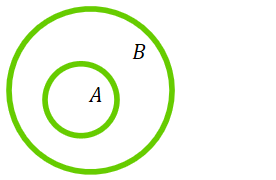
\includegraphics{../Mathematik_1/Bilder/mengen_echte_teilmenge.png} %Diagramm / Beispiel
\end{minipage}
\begin{minipage}{0.7\textwidth}
	\begin{itemize} 
	\item \(A\) ist eine Teilmenge von \(B\): \(A\subseteq B\)
	\item \(B\) ist eine Obermenge von \(A\): \(A\subseteq B\)
	\item \(A\) ist nicht gleich \(B\): \(A\not = B\)
	\item \(A\) ist eine \textbf{echte} Teilmenge von \(B\): \(A\subsetneq B\)
\end{itemize}
\end{minipage}
\end{exabox}
  
Zwei Mengen \(A\) und \(B\) sind gleich, \(A=B\), wenn sie dieselben Elemente enthalten. 

In der Mengenlehre gibt es vier grundlegende Mengenoperationen, n�mlich: Vereinigung, Schnitt, Differenz und Komplement: 

\begin{exabox}{Mengenoperationen}{}
	\begin{itemize}
		\item Die Vereinigung  (\emph{union}) zweier Mengen wird mit dem Symbol \(\cup\) angezeigt. Die Vereinigungsmenge enth�lt jedes Element der beiden Mengen genau einmal, beispielsweise
	\[ \{ 1, 2, 4\} \cup \{2, 5, 3, 4\} = \{1,2,3,4,5\}\,. \]
\item Der Schnitt (\emph{intersection}) zweier Mengen wird mit dem Symbol \(\cap\) angezeigt. Die Schnittmenge enth�lt jedes Element, das in beiden Mengen vorkommt, beispielsweise 
	\[ \{ 1, 2, 4\} \cap \{2, 5, 3, 4\} = \{2,4\}\,. \]
\item Die Differenz (\emph{difference}) zweier Mengen wird mit einem Backslash angezeigt. Die Differenzmenge enth�lt jedes Element, das in der ersten Menge vorkommt, aber nicht in der zweiten, beispielsweise 
	\[ \{ 1, 2, 4\} \setminus \{2, 5, 3, 4\} = \{1\}\,.\]
\item Das Komplement (\emph{complement}) einer Menge \(A\) wird mit einem waagerechten Strich �ber der Menge angezeigt, also \(\overline A\). Ist eine Obermenge \(B\) von \(A\) fixiert, dann bedeutet das Komplement \(\overline A\) die Differenz von Obermenge \(B\) und \(A\). Aus der Schreibweise \(\overline A\) geht die Obermenge nicht hervor - die Obermenge muss also implizit bekannt sein! Im folgenden Beispiel ist die Obermenge die Menge der nat�rlichen Zahlen ohne die Null, also $\mathbb N = \{ 1, 2, 3, 4, 5, 6, \dots\}$: 
	\[ \overline{\{2, 4, 6, 8\}} = \mathbb N \setminus \{2, 4, 6, 8\} = \{1,3,5,7\} \cup \{9,10,11,12, \dots\}\,. \]
	\end{itemize}
\end{exabox}

Neben den bisher betrachteten Mengenoperationen gibt es eine weitere wichtige M�glichkeit, aus gegebenen Mengen eine neue Menge zu bilden. Dabei werden die Elemente der beiden Mengen nicht vereinigt oder miteinander verglichen, sondern zu \textbf{geordneten Paaren} zusammengesetzt.

F�r zwei Mengen \(A\) und \(B\) hei�t

$$
A\times B
=
\{(a,b):a\in A \text{ und } b\in B\}
$$

das kartesische Produkt (\emph{cartesian product}) von \(A\) und \(B\).

Anders als bei den Elementen einer Menge spielt innerhalb eines geordneten Paares die Reihenfolge eine Rolle. Im Allgemeinen gilt daher

$$
(a,b)\neq(b,a).
$$

Das passt zu dem bereits bekannten Unterschied zwischen Mengen und Tupeln: W�hrend beispielsweise

$$
\{2,3\}=\{3,2\}
$$

gilt, sind die geordneten Paare

$$
(2,3)\neq(3,2)
$$

verschieden.

\begin{exabox}{Kartesisches Produkt}{ }
F�r

$$
A=\{\circ,\diamond,M\}
\qquad\text{und}\qquad
B=\{3,7\}
$$

ergibt sich

$$
\begin{aligned}
A\times B
=
\{&
(\circ,3),(\circ,7),
(\diamond,3),(\diamond,7),\\
&
(M,3),(M,7)
\}.
\end{aligned}
$$

Jedes Element aus \(A\) wird dabei mit jedem Element aus \(B\) kombiniert.
\end{exabox}

Besonders wichtig ist das kartesische Produkt einer Menge mit sich selbst. F�r die reellen Zahlen gilt beispielsweise

$$
\mathbb R^2
:=
\mathbb R\times\mathbb R
=
\{(x,y):x\in\mathbb R \text{ und } y\in\mathbb R\}.
$$

Die Elemente von \(\mathbb R^2\) sind also geordnete Paare reeller Zahlen. Sie k�nnen geometrisch als Punkte der Ebene interpretiert werden.

Entsprechend entstehen durch weitere kartesische Produkte geordnete Tripel und allgemein geordnete \(n\)-Tupel. Beispielsweise ist

$$
\mathbb R^3
=
\{(x,y,z):x,y,z\in\mathbb R\}
$$

die Menge aller geordneten Tripel reeller Zahlen und kann als Menge der Punkte des dreidimensionalen Raumes aufgefasst werden.
  
Entsprechend zu "\,Punktrechnung vor Strichrechnung"\, wird der Schnitt vor der Vereinigung ausgef�hrt:
\begin{theorembox}{Rechenregel: Schnitt vor Vereinigung}{ }
$  A \cup B \cap C = A \cup \left( B \cap C\right) \,.  $
\end{theorembox}

\subsection{Was ist eine mathematische Aussage?}

Eine  mathematische Aussage (\emph{statement,  proposition}) ist eine Aussage, der man einen Wahrheitswert zuordnen kann. Entweder ist die Aussage wahr (\emph{true}) oder falsch (\emph{false}). Eine mathematische Aussage kann aus diesem Grund \textbf{keine} freien Variablen enthalten. Wenn freie Variablen vorkommen, handelt es sich um ein Pr�dikat. Man nennt ein Pr�dikat auch "\,eine Aussageform"\, oder einfach "\,ein mathematischer Ausdruck"\,:
  
\begin{exabox}{Aussagen und Pr�dikate}{ }
  \begin{itemize}
  \item "$2^2 = 5$"\, ist eine falsche Aussage.
    \item "$2^2 \not= 5$" \; ist eine wahre Aussage.
    \item "$x^2 \in \mathbb N$" \; ist ein Pr�dikat.
  \end{itemize}
\end{exabox}

  
\begin{exabox}{Aussagen}{ }
  \begin{itemize}
	  \item "\,F�r eine beliebige nat�rliche Zahl $x\in \mathbb N$ gilt $x^2 \in \mathbb N$"\; ist eine wahre Aussage.
	  \item "\,F�r eine beliebige rationale Zahl $x\in \mathbb Q$ gilt  $x^2 \in \mathbb N$"\; ist eine falsche Aussage.
  \end{itemize}
\end{exabox}
Mathematische Aussagen treten selten isoliert auf. H�ufig m�chte man Aussagen \textbf{verneinen} oder mehrere Aussagen miteinander \textbf{verkn�pfen}. Auch daf�r besitzt die Mathematik eine eigene Kurzschreibweise.

Beginnen wir mit der Negation oder Verneinung. Betrachten wir die Aussage

$$
p:\qquad x\geq 0.
$$

Diese Aussage ist beispielsweise f�r \(x=3\) wahr und f�r \(x=-2\) falsch. M�chte man genau das Gegenteil von \(p\) ausdr�cken, so lautet die entsprechende Aussage:

$$
q: \qquad x<0.
$$

In Worten k�nnte man auch sagen: �Es gilt \textbf{nicht} \(x\geq0\).�

Die Aussage \(q\) ist die Negation (\textit{negation}) von \(p\) und das l�sst sich in mathematischer Formelsprache mit Hilfe des Symbols \(\neg\) ausdr�cken: die Negation von \(p\) ist 

$$
\neg p.
$$

Eine Negation \(\neg p\) ist genau dann wahr, wenn die urspr�ngliche Aussage \(p\) falsch ist -- und umgekehrt.

\begin{exabox}{Negation einer Aussage}{ }
	\begin{itemize}
\item F�r $ \; p:\qquad x\geq 0\; $ lautet die Negation $ \;\neg p:\qquad x<0$.
\item Beispielsweise ist f�r \(x=-2\) die Aussage \(p\) falsch und die Aussage \(\neg p\) wahr.
	\end{itemize}
\end{exabox}

Neben der Negation einer einzelnen Aussage m�chte man Aussagen auch miteinander verbinden. Betrachten wir beispielsweise die Aussage \( p:\; x>2\) und die Aussage \(q:\; x<5\). Suchen wir alle reellen Zahlen, f�r die \textbf{sowohl}  \(p\) \textbf{als auch} \(q\) gleichzeitig wahr ist, so verkn�pfen wir die Aussagen durch ein logisches �und�. In mathematischer Formelsprache ist das logische �und� das Symbol \(\land\):

$$
p\land q: \qquad x>2 \;\textnormal{und gleichzeitig} \; x<5.
$$
Eine Und-Verkn�pfung (\emph{and}) \(p\land q \) ist genau dann wahr, wenn sowohl \(p\) als auch \(q\) wahr sind.

Suchen wir alle reellen Zahlen, f�r die \textbf{mindestens eine der Aussagen}, wahr ist, so verkn�pfen wir die Aussagen durch ein logisches �oder� . In mathematischer Formelsprache ist das logische �oder�  das Symbol \(\lor\): 

$$
p\lor q: \qquad x>2 \;\textnormal{oder}\; x<5.
$$
Eine Oder-Verkn�pfung (\emph{or}) \(p\land q \) ist genau dann wahr, wenn  mindestens eine der beiden Aussagen \(p\) und \(q\) wahr ist.

\begin{exabox}{Und und Oder lesen}{ }
	Es seien $ p:\; x>2$ und $q:\; x<5 $.
	\begin{itemize}
		\item $ p\land q $ bedeutet in Worten  �\(x\) ist gr��er als \(2\) und gleichzeitig kleiner als \(5\).� und  diese Aussage ist  genau dann wahr wenn $ 2<x<5 $.  
		\item $ p\lor q $ bedeutet in Worten  �\(x\) ist gr��er als \(2\) oder kleiner als \(5\).� und diese Aussage ist genau dann wahr wenn \(x>2\) oder \(x<5\) wahr ist, wobei auch beide Bedingungen gleichzeitig erf�llt sein d�rfen (aber nicht m�ssen).
	\end{itemize}
\end{exabox}

\noindent{\textbf{Bemerkungen:}}
\begin{itemize}
	\item Die Symbole \(\neg\), \(\land\) und \(\lor\) werden uns immer wieder begegnen. Sie sind nicht nur Bestandteil der Aussagenlogik, sondern geh�ren zur mathematischen Formelsprache. 
	\item Bei der Beschreibung von Mengen werden wir Bedingungen mit diesen Operatoren sinnvoll verkn�pfen. Deshalb ist es wichtig, logische Ausdr�cke nicht nur selbst aufschreiben, sondern auch in nat�rliche Sprache �bersetzen zu k�nnen.
	\item Beim mathematischen Oder ist das Wort �oder� einschlie�lich zu verstehen: Sind \(p\) und \(q\) beide wahr, dann ist auch \(p\lor q\) wahr. Das unterscheidet das mathematische Oder von Formulierungen wie �entweder -- oder�, bei denen h�ufig gemeint ist, dass genau eine von zwei M�glichkeiten eintreten soll.
\end{itemize}

Entsprechend zu �Punktrechnung vor Strichrechnung� gibt es auch f�r logische Operatoren eine festgelegte Reihenfolge: Zuerst wird die Negation ausgef�hrt, danach das Und und zuletzt das Oder.

\begin{exabox}{Klammern weglassen?}{ }
Betrachten wir den vollst�ndig geklammerten Ausdruck

$$
\bigl(\neg(x\geq 6)\bigr)\lor\bigl((x\geq 10)\land(x<20)\bigr).
$$

Welche Klammern k�nnen weggelassen werden, ohne die Bedeutung des Ausdrucks zu ver�ndern?

Da die Negation \(\neg\) vor dem Und \(\land\) und das Und vor dem Oder \(\lor\) ausgef�hrt wird, kann man k�rzer schreiben:

$$
\neg(x\geq6)\lor (x\geq10)\land(x<20).
$$

Die Klammer um \(x\geq6\) bleibt stehen, da sich die Negation auf die gesamte Aussage \(x\geq6\) bezieht.
\end{exabox}

Liest man zwischen zwei Ausdr�cken \(p\) und \(q\) das Symbol $"\Rightarrow"$, dann ist das Konstrukt \( p\Rightarrow q\)  eine logische Schlussfolgerung oder Implikation. Ein Beispiel: 
\begin{exabox}{Schlussfolgerung (Implikation)}{ }
  $ x \geq 7 \Rightarrow x > 5$
\end{exabox}

Mit Worten liest man die Implikation \("p\Rightarrow q"\) wie folgt:
\begin{itemize}
	\item aus $p$ folgt $q$,
	\item wenn $p$ wahr ist, dann ist $q$ wahr,
	\item die G�ltigkeit von $p$ reicht aus \footnote{�fter - aber irgendwie verwirrend - ist hinreichend} (\emph{sufficient}) f�r die G�ltigkeit von \(q\),
\end{itemize}

Es ist wichtig zu bemerken, dass man die Reihenfolge der Ausdr�cke \(p\) und \(q\) in einer Implikation nicht vertauchen darf:
\begin{exabox}{Implikation ist keine kommutative Verkn�pfung}{ }
	Es regnet $\begin{array}{c}\Rightarrow \\\not \Leftarrow\end{array}$ Der Himmel ist bew�lkt.
\end{exabox}



Liest man zwischen zwei Aussagen \(p\) und \(q\) das Symbol \(\Leftrightarrow\), dann handelt es sich um eine �quivalenz. Die Schreibweise

$$
p\Leftrightarrow q
$$

bedeutet, dass \(p\) und \(q\) immer denselben Wahrheitswert besitzen: Entweder sind beide Aussagen wahr oder beide Aussagen sind falsch.\footnote{Das �quivalenzzeichen ist damit f�r die Logik das, was das Gleichheitszeichen \(=\) f�r die Algebra ist.}

�quivalenzen treten beispielsweise beim Umformen von Gleichungen auf. Wird eine Gleichung durch �quiva\-lenz\-umformungen gel�st, dann beschreiben die einzelnen Zeilen jeweils dieselbe L�sungsmenge:

\begin{exabox}{�quivalenz beim L�sen einer Gleichung}{ }

$$
3x-1=2
\quad\Leftrightarrow\quad
3x=3
\quad\Leftrightarrow\quad
x=1
\quad\Leftrightarrow\quad
\mathbb L=\{1\}.
$$

\end{exabox}

Eine �quivalenz kann aber auch zwei unterschiedlich formulierte Aussagen miteinander verbinden:

\begin{exabox}{�quivalenz beim L�sen einer Gleichung}{ }

$$
x^2=4
\quad\Leftrightarrow\quad
x\in\{-2,2\}.
$$

\end{exabox}

Warum darf hier tats�chlich ein �quivalenzpfeil stehen? Daf�r m�ssen beide Richtungen der Aussage gelten.

Von links nach rechts ist zu zeigen:

$$
x^2=4
\quad\Rightarrow\quad
|x|=2
\quad\Rightarrow\quad
x=\pm2
\quad\Rightarrow\quad
x\in\{-2,2\}.
$$

Von rechts nach links ist zu zeigen:

$$
x\in\{-2,2\}
\quad\Rightarrow\quad
x=-2\ \lor\ x=2
\quad\Rightarrow\quad
x^2=4.
$$

Eine �quivalenz

$$
p\Leftrightarrow q
$$

besteht also aus zwei Schlussfolgerungen:

$$
p\Rightarrow q
\qquad\text{und}\qquad
q\Rightarrow p.
$$

Um eine �quivalenz nachzuweisen, m�ssen daher immer beide Richtungen gelten.

Mit Worten liest man die �quivalenz \( p \Leftrightarrow q\) wie folgt: 
\begin{itemize}
  \item $p$ ist genau dann wahr, wenn $q$ wahr ist, 
  \item $p$ gilt dann und nur dann, wenn $q$ gilt (\emph{$p$ if and only if $q$}),
  \item $p$ ist notwendig und hinreichend (\emph{necessary and sufficient}) f�r $q$.  
\end{itemize}

\subsection{Mengen und Aussagen}

Der Gedanke, mit dem wir den Abschnitt eingeleitet haben, klang so, als w�ren Mengen von extremer Bedeutung in der Mathematik: "\,Mengen sind die Grundlage aller mathematischen Objekte."\, Die Mengen, die wir bislang notiert haben, hatten alle weniger als f�nf Elemente und scheinen diese Bedeutung nicht widerzuspiegeln. Mit den Begriffen der Logik haben wir jetzt das Werkzeug an der Hand, um nochmal �ber Mengen nachzudenken und um zu verstehen, dass sie Grundlage der mathematischen Fachsprache sind. 

Was ist eine Menge nochmal? Eine Menge ist eine Ansammlung von Objekten. Kennt man alle Objekte, dann kennt man die Menge - oder anders ausgedr�ckt: man kennt eine Menge, wenn man von einem Objekt sagen kann, ob es zur Menge geh�rt oder nicht. 

Zwei Varianten, die es zulassen zu entscheiden, ob ein Objekt dazugeh�rt oder nicht sind die folgenden: 
\begin{itemize}
	\item Die Menge bzw. deren Elemente sind explizit gegeben. Eine Menge in \textbf{expliziter} Schreibweise lautet beispielsweise so:
\[ M = \{0,1,2,3,4,5,6,7,8,9\}\,, \]
	\item Die Menge wird mit Worten beschrieben. Eine Menge in sogenannter \textbf{intensionaler} Schreibweise lautet beispielsweise so: 
		\[ M = \{ \textnormal{Menge aller nat\"urlichen Zahlen, die kleiner als zehn sind.}\} \]
\end{itemize}
Etwas umst�ndlicher, aber gleichbedeutend ist  
\[ M = \{ \textnormal{Alle Zahlen } \textcolor{blue}{x\,, \textnormal{f\"ur gilt: }} \textcolor{darkgreen}{ x \textnormal{ ist nat\"urlich und } x \textnormal{ ist kleiner als zehn.}}\ \}  \]  
Diese Beschreibung ist zwar verst�ndlich, aber f�r mathematische Texte unn�tig umst�ndlich. Sie l�sst sich unmittelbar in mathematischer Formelsprache �bersetzen. 
\[ M =  \{ \textcolor{blue}{x:} \; \textcolor{darkgreen}{x\in\mathbb N_0 \land x< 10} \}\,. \]  
\begin{itemize}
	\item Das Fragment "\,Alle Zahlen"\,, mit dem die Beschreibung der Menge startet, wurde einfach weggelassen.  
	\item Anstatt "\( x\), f�r die gilt:"\, schreibt man "\( x:\)".\footnote{ manchmal auch "\( x\;|\)".} 
	\item Und "\(x\) ist nat\"urlich und \(x\) ist kleiner als zehn"\, �bersetzt man in mathematische Kurzschreibweise, also "\(x\in\mathbb N_0 \land x<10\)".
\end{itemize}

\noindent{\textbf{ Bemerkungen:}}
\begin{itemize}
	\item Wenn die Menge, die man betrachtet, eine Teilmenge einer bekannten Grundmenge\footnote{\(\mathbb N_0, \mathbb Z, \mathbb Q, \mathbb R, \mathbb C, \cdots\)} ist, beispielsweise eine Teilmenge der nat�rlichen Zahlen, dann schreibt man diese Grundmenge auch oft \textbf{vor} die Zusatzbedingung, also 
\[ M =  \{ x\in \mathbb N_0: x< 10 \}\,. \]  
	\item "\,Bedingung erf�llen"\, bedeutet in der Aussagenlogik, dass eine Aussage wahr wird. Mit Bedingung sind sich all die Eigenschaften gemeint, die die Elemente der Menge haben sollen. 
	\item Oft erf�llen die Elemente einer Menge mehrere Bedingungen und ob die Bedingungen alle gleichzeitig erf�llt sein m�ssen, oder ob eine Bedingung ausreicht, l�sst sich mit Hilfe der Operatoren \(\land\) und \(\lor\) pr�zise angeben.     
\end{itemize}

Mengen beschreibt man also im Allgemeinen mit Hilfe von logischen Ausdr�cken. Hier ein paar Beispiele:
\begin{exabox}{Mengen in mathematischer Kurzschreibweise}{ }
	\begin{itemize}
		\item Die Menge aller reellen Zahlen zwischen $3$ (einschlie�lich) und $5$ (ausschlie�lich)
			\[ M = \{ x \in \mathbb R: x \geq 3 \land x < 5 \} = \{ x \in \mathbb R: 3\leq x < 5 \}\,, \]
		\item Die obere H�lfte der Kreisscheibe ohne Rand. Die Kreisscheibe besitze Radius \(R=1\) und Mittelpunkt \( (0|0)\):
			\[M = \{ (x,y) \in \mathbb R^2: y \geq 0 \land x^2+y^2 < 1\}\,. \]
		\item Streng genommen muss man die Grundmenge angeben, aus der die Elemente zu nehmen sind:
	\[ 
	\begin{array}{rcl}
		\left\{ x \in \mathbb Q: x^2 = 2\right\} &=& \emptyset \,, \\ [1ex]
 \left\{ x \in \mathbb R: x^2 = 2\right\} &=& \left\{ -\sqrt{2}, \sqrt{2} \right\}\,.  
\end{array}
\]
\end{itemize}
\end{exabox}

Um komplexe Konstruktionen solcher Art mathematisch wasserdicht zu machen, muss man von der naiven Mengenlehre zur axiomatischen Mengenlehre �bergehen. Dass ein axiomatischer Zugang n�tig ist, sieht man am Beispiel \href{https://de.wikipedia.org/wiki/Russellsche_Antinomie}{der Russellschen Antinomie }. In der Praxis kommt man mit der naiven Mengenlehre zurecht.

Wenn man Schlussfolgerungen 
\begin{itemize} 
	\item f�r alle Elemente einer Menge treffen m�chte, dann benutzt man in der mathematischen Kurzschreibweise das Symbol $"\forall"$. \(\forall\) ist ein \emph{Quantor} und man �bersetzt ihn mit den Worten "\,f�r alle",
	\item f�r ein Element einer Menge treffen m�chte, dann benutzt man in der mathematischen Kurzschreibweise das Symbol $"\exists"$. \(\exists\) ist ein Quantor und man �bersetzt ihn mit den Worten "\,es existiert (mindestens) ein".
\end{itemize}

\begin{exabox}{Quantoren $\forall$ und $\exists$}{ }
	\begin{itemize}
		\item $A = \{2,4,6\} \; \Rightarrow\; \forall\, x \in A: \dfrac{x}{2} \in \mathbb N^+ .$
		\item $B = \{-3, 2,4,6\} \; \Rightarrow \; \exists\; x \in B: \; x<0 \,.$
	\end{itemize}
\end{exabox}
Ein Quantor hat noch eine weitere wichtige Funktion: Er \textbf{bindet} eine Variable. Betrachten wir beispielsweise das Pr�dikat

$$
p:\qquad x^2\geq 0.
$$

Solange nicht festgelegt ist, f�r welche Zahl \(x\) die Bedingung betrachtet wird, besitzt dieser Ausdruck keinen eigenen Wahrheitswert. Es handelt sich um ein Pr�dikat und noch nicht um eine Aussage.

Erst, wenn man f�r \(x\) einen konkreten Wert annimmt, beispielsweise \(x=-2\), dann entsteht eine Aussage. Beispielsweise ist

$$
p:\qquad (-2)^2\geq0
$$

eine wahre Aussage.

Eine Aussage entsteht aber auch, wenn die Variable durch einen Quantor gebunden wird. So ist

$$
\forall\,x\in\mathbb R:\quad x^2\geq0
$$

eine wahre Aussage. Sie bedeutet: �F�r jede reelle Zahl \(x\) gilt \(x^2\geq0\).�

Auch

$$
\exists\,x\in\mathbb R:\quad x^2=4
$$

ist eine Aussage. Sie bedeutet: �Es gibt mindestens eine reelle Zahl \(x\), f�r die \(x^2=4\) gilt.� Diese Aussage ist ebenfalls wahr.

Ein Pr�dikat wird also zu einer Aussage, wenn f�r die vorkommenden freien Variablen konkrete Werte eingesetzt werden oder wenn die freien Variablen beispielsweise durch Quantoren gebunden werden. Erst dann l�sst sich der entstandenen Aussage eindeutig ein Wahrheitswert zuordnen.

Bei der Negation von Aussagen mit Quantoren ist besondere Vorsicht notwendig. Betrachten wir beispielsweise die Aussage

$$
\text{�Alle Zahlen in der Menge \(M=\{2,4,6,7\}\) sind gerade.�}
$$

Um zu zeigen, dass diese Aussage falsch ist, m�ssen nicht alle Elemente der Menge untersucht und verneint werden. Es gen�gt, ein einziges Element zu finden, das nicht gerade ist. Hier ist \(7\) ein solches Element. Die Negation der Aussage lautet daher:

$$
\text{�Es gibt mindestens eine Zahl in \(M\), die nicht gerade ist.�}
$$

In mathematischer Kurzschreibweise wird aus

$$
\forall\,x\in M:\quad x\text{ ist gerade}
$$

bei der Negation also

$$
\exists\,x\in M:\quad x\text{ ist nicht gerade}.
$$

Die Negation einer Aussage mit dem Quantor \(\forall\) f�hrt zu einer Aussage mit einem Existenzquantor \(\exists\).

Umgekehrt funktioniert derselbe Gedanke. Die Aussage

$$
\text{�Es gibt mindestens eine Zahl in \(M\), die ungerade ist.�}
$$

ist genau dann falsch, wenn keine einzige Zahl in \(M\) ungerade ist. Ihre Negation lautet daher:

$$
\text{�Alle Zahlen in \(M\) sind nicht ungerade.�}
$$

Beim Negieren wird also aus dem Existenzquantor \(\exists\) ein Allquantor \(\forall\) und gleichzeitig wird die zugeh�rige Aussage negiert.

Allgemein gilt:

\begin{theorembox}{Negation quantifizierter Aussagen}{ }

$$
\begin{array}{rcl}
\neg\left(\forall\,x\in M:\;p(x)\right)
&\Leftrightarrow&
\exists\,x\in M:\;\neg p(x),
\\[1ex]
\neg\left(\exists\,x\in M:\;p(x)\right)
&\Leftrightarrow&
\forall\,x\in M:\;\neg p(x).
\end{array}
$$

\end{theorembox}

In Worten bedeutet dies:

$$
\text{�Nicht alle erf�llen \(p\)�}
\quad\Leftrightarrow\quad
\text{�Mindestens eines erf�llt \(p\) nicht�,}
$$

und

$$
\text{�Es gibt keines, das \(p\) erf�llt�}
\quad\Leftrightarrow\quad
\text{�Alle erf�llen \(p\) nicht�.}
$$

\begin{exabox}{Mathematische Kurzschreibweise}{ }
Wie lauten die Definitionen f�r "\,gleiche Mengen"\, oder "\,Mengenoperationen"\, in mathematischer Kurzschreibweise?
	\begin{itemize}
		\item Zwei identische Mengen: \[ A = B: \, \Leftrightarrow\; A\subset B \land B \subset A \;\Leftrightarrow \; \left( \forall \, x \in A: \; x \in B\right) \land \left( \forall \, x \in B: \; x \in A\right)\,. \]
		\item Die Vereinigungsmenge:
			\[  A \cup B = \{ x:\; x \in A \lor x \in B\}\,.\]
		\item Die Schnittmenge:
			\[ A \cap B = \{ x:\; x \in A \land x \in B\}\,. \]
		\item Die Differenzmenge:
			\[ A \setminus B = \{x:\; x\in A \land x \not\in B \}\,. \]
		\item Die Komplementmenge (bei gegebener Menge $B$ und bekannter Obermenge $A$ mit $B\subset A$):
			\[ \overline B = \{ x: x\in A\land x\not \in B\}\,. \]
	\end{itemize}
\end{exabox}

\subsubsection*{Rechenregeln f�r Mengen und Aussagenlogik}

Man kann sagen, dass es zu jedem Mengenoperator einen logischen Operator gibt, der ihm algebraisch entspricht. In der Elektronik muss man logische Operatoren realisieren und das macht man durch Reihen- und/oder Parallelschaltungen. Eine detaillierte �bersicht �ber Logikgatter findet man \href{https://de.wikipedia.org/wiki/Logikgatter}{hier} und die Kurzvariante ist
\begin{center}
  \begin{tabular} {c c c c c }
	  Mengen &  &  Logik & & Elektronik\\
  \hline
  $\cap$ & $ \widehat = $ & $\land$ & $ \widehat = $ & Serie-Schaltung \\
  $\cup$ & $ \widehat = $ &  $\lor$ & $\widehat = $& Parallel-Schaltung\\
  $\overline{\{\}}$ & $ \widehat = $ &  $\neg$ & & \ldots\\
\end{tabular}
\end{center}

Logik "\,unterliegt"\, strengen Gesetzm��igkeiten und wenn man diese kennt, dann wird das "\,logische Argumentieren"\, einfacher:
\begin{theorembox}{Assoziativgesetze und die de Morgansche Gesetze}{ }
  \begin{center}
  \begin{tabular}{c|c|c|c}
  Name & Mengen & Logik & Bedeutung\\
  \hline
  \hline
  \multirow{2}{*}{Assoziativgesetze} & $ (A\cap B) \cap C = A\cap (B \cap C) $ & $ (p \land q) \land r \Leftrightarrow p \land (q \land r)$ & \multirow{2}{*}{ Reihenfolge egal}\\[1ex]
  & $ (A\cup B) \cup C = A\cup (B \cup C) $ & $ (p \lor q) \lor r \Leftrightarrow p \lor (q \lor r)$  & \\[2ex]
  \hline
  \multirow{2}{*}{De Morgansche Gesetze} & $ \overline {A\cap B}  = \overline A\cup  \overline B $ & $  \neg \, ( p \land q)  \Leftrightarrow \neg p \lor \neg q$ & \multirow{2}{*}{Logik der Negation} \\[1ex]
  & $ \overline {A\cup B}  = \overline A\cap  \overline B $ & $  \neg \, ( p \lor q)  \Leftrightarrow \neg p \land \neg q$ &
\end{tabular}
\end{center}
\end{theorembox}

Um die De Morganschen Gesetze zu beweisen, kann man eine Wahrheitstabelle aufstellen! Die Idee ist den logischen Ausdruck $\neg\, (p \land q)$ in Teilaussagen zu zerlegen und dann alle m�glichen F�lle zu betrachten\footnote{Die m�glichen F�lle sind immer  entweder "\,wahr"\, oder "\,falsch"\,, also �berschaubar in Komplexit�t!}: 

\begin{exabox}{Wahrheitstabelle zum Beweis des $1.$ Morganschen Gesetzes}{ }
  \begin{center}
  \begin{tabular}{cc||c|>{\columncolor[gray]{0.9}} c|c|c|>{\columncolor[gray]{0.9}}c} 
	  Input $p$ &  Input $q$ & Output $p\land q$ & Output $\neg (p \land q)$ & Output $\neg p $ & Output $\neg q $ & Output $\neg p \lor \neg q$ \\  
  \hline
  f & f & f & w & w & w & w\\ 
  f & w & f & w & w & r & w\\ 
  w & f & f & w & f & w & w\\ 
  w & w & w & f & f & f & f
\end{tabular}
\end{center}
\end{exabox}
  % Mengen und Logik
\newpage
\setcounter{satz}{0} \setcounter{def}{0} \setcounter{exa}{0}  \section{Zahlenmengen}\label{MA1-zahlenmengen}

\begin{table}[H]
  \centering
  \begin{tabularx}{\textwidth}{p{0.9\textwidth} p{0.1\textwidth}}
    \toprule
	  \multicolumn{2}{c}{\textbf{�bersicht �ber Lernziele und Voraussetzungen}}\\
    \midrule
	  \textbf{Lernziele} &\\[.5\normalbaselineskip]
    \tabitem die Zahlenmengen \(\mathbb N_0, \mathbb N^+, \mathbb Z, \mathbb Q\) unterscheiden und korrekt verwenden &\\
    \tabitem die wesentlichen Eigenschaften eines K�rpers am Beispiel von
\(\mathbb Q\) und \(\mathbb R\) erkl�ren & \\
    \tabitem Fakult�ten und Binomialkoeffizienten berechnen &\\
    \tabitem Rechengesetze in \(\mathbb R\) sicher anwenden &\\
    \tabitem Summen- und Produktsymbole ausschreiben und vereinfachen &\\
    \tabitem den Binomischen Satz anwenden &\\
    \midrule
	  \textbf{Voraussetzungen} \\[.5\normalbaselineskip]
    \tabitem Grundrechenarten &\\
    \bottomrule
  \end{tabularx}
\end{table}

\ifintegriereaufgaben \noindent �bungsaufgaben zum Thema finden Sie hier: \hyperref[MA1-zahlenmengen-aufgaben]{Aufgaben}
\vspace{0.3cm}
\hrule
\fi

\subsection{Nat�rliche, ganze und rationale Zahlen}

Zum Z�hlen ben�tigt man die Zahlen $1,  2,  3,\dots$. Diese Menge von Zahlen nennt man die \textbf{nat�rlichen Zahlen} (\emph{natural numbers}) und f�hrt das Symbol \(\mathbb N\) ein. Allerdings ist unklar, ob \(\mathbb N\) die Null beinhaltet oder nicht\footnote{In der Informatik z�hlt die Null meist dazu und in der Mathematik mal so mal so.} In diesem Skript werden Indizes eingef�hrt, die die Frage pr�zise kl�ren: $\mathbb N_0$ enth�lt die Null und $\mathbb N^+$ nicht.\footnote{Wie lauten die Bedingungen in mathematischer Kurzschrift? \(0\in \mathbb N_0\) und \( \forall n\in \mathbb N^+: n>0\).}

Im Zahlenbereich $\mathbb Z$ der  \textbf{ganzen Zahlen}  (\emph{integers}) kommen die negativen ganzen Zahlen hinzu. 

Kommen noch alle positiven und negativen Br�che hinzu, erh�lt man den Bereich der \textbf{rationalen Zahlen} \(\mathbb Q\) (\emph{rational numbers}).

\begin{defbox}{Nat�rliche, ganze und rationale Zahlen: $\mathbb N$, $\mathbb Z$ und $\mathbb Q$}{ }
\begin{eqnarray*}
	\mathbb N_0 &=& \{ 0,1,2,3, 4\dots \}\,, \\
	\mathbb N^+ &=&  \{ 1,2,3, 4\dots \}\,, \\
	\mathbb Z &=& \left\{ \dots,-3,-2,-1,0,1,2,3,\dots \right\} = \mathbb N_0 \cup \{-1,-2,-3,-4,\cdots\}\,,\\
   \mathbb Q &=& \left\{ \displaystyle{\frac{m}{n}}, \quad m \in \mathbb Z \land n \in \mathbb N^+\right\}\,.
  \end{eqnarray*}
\end{defbox}

Wenn eine Rechenoperation in der Mathematik immer wieder auftaucht, dann ist es sinnvoll ein Symbol einzuf�hren. Solche zwei Rechenoperationen mit nat�rlichen Zahlen sind die Fakult�t und der Binomialkoeffizient.\marginpar{\small Aufgabe} Sie sind wie folgt definiert:   

\begin{defbox}{Fakult�t und Binomialkoeffizient}{ }
	\begin{center}
	\begin{tabular}{l|l|l|l}
Name & Symbol & Wertebereich &  Besonderheit  \\
\hline
Fakult�t & \(n! = n\cdot (n-1) \cdot (n-2)  \dots  1 \) & \(n\in \mathbb N_0\) &  \(0! = 1! = 1\) \\[2ex]
Binomialkoeffizient &  \(\displaystyle{\binom{n}{k}} = \displaystyle{\frac{ n!}{ k!\cdot (n-k)!}} \) & \( n,k\in\mathbb N_0 : \;k\leq n \)    & \( \displaystyle{\binom{n}{0}} = \displaystyle{\binom{n}{n}} = 1  \)
\end{tabular}
\end{center}
\end{defbox}

\noindent {\textbf{ Bemerkungen: }}
\begin{itemize}
	\item Die Anzahl der M�glichkeiten $n$ verschiedene Objekte in einer Reihe anzuordnen ist \(n\)-Fakult�t.
	\item Die Anzahl der M�glichkeiten aus einer $n$-elementigen Menge $k$ Elemente auszuw�hlen ist \(n\) �ber \(k\).
\end{itemize}

\subsection{Reelle Zahlen}


Um $x^{2}=2$ l�sen zu k�nnen oder den Umfang eines Kreises mit Durchmesser $1$ als Zahl anzugeben, ben�tigt man einen gr��eren Zahlenbereich: den der \textbf{reellen Zahlen} $\mathbb R$ (\emph{real numbers}). 

\begin{exabox}{Reelle Zahlen}{ }
	$\displaystyle{\left\{-\ln(77)\,, \; \sqrt{2}\,, \; \pi\,, \; \frac{4}{28}\,, \; 38624983 \right\} \subset \mathbb R\,. }$
\end{exabox}

Die reellen Zahlen besitzen gegen�ber den rationalen Zahlen eine weitere wichtige Eigenschaft: Sie sind \textbf{vollst�ndig}\footnote{Vereinfacht gesprochen bedeutet die Vollst�ndigkeit von \(\mathbb R\): Konvergente N�herungsverfahren, deren Werte reelle Zahlen sind und die sich immer weiter auf einen Wert festlegen, f�hren nicht aus dem Zahlenbereich \(\mathbb R\) hinaus.} Anschaulich bedeutet dies, dass der reelle Zahlenstrahl keine �L�cken� besitzt. Eine solche L�cke tritt beispielsweise auf, wenn man versucht, \(\sqrt{2}\) ausschlie�lich mit rationalen Zahlen zu erfassen. Durch immer genauere rationale N�herungen kann man sich der Zahl \(\sqrt{2}\) beliebig weit ann�hern. Der Grenzwert dieser N�herungen ist jedoch selbst keine rationale Zahl. Innerhalb von \(\mathbb Q\) fehlt also genau die Zahl, auf die die N�herungen zulaufen.

\begin{exabox}{Die Zahl \(\sqrt{2}\)}{ }
Ein klassisches Beispiel f�r eine reelle Zahl, die nicht rational ist, ist \(\sqrt{2}\). Angenommen, es g�be einen vollst�ndig gek�rzten Bruch

$$
\sqrt{2}=\frac pq,\qquad p,q\in\mathbb N^+.
$$

Dann folgt

$$
	\begin{array}{rcrcl l} 
		\sqrt{2}=\dfrac pq & \Rightarrow & 2\cdot q^2 &=& p^2 & \Rightarrow p^2\text{ gerade}, p\text{ gerade}\\
		&\Rightarrow & \exists \, k \in \mathbb N^+: \,  p &=& 2\cdot k \\
		&\Rightarrow & 2\cdot q^2=&=& 4\cdot k^2 & \\  & \Leftrightarrow & q^2 &=& 2 \cdot k^2  &\Rightarrow q^2\text{ gerade}, \, q\text{ gerade}.
\end{array}
$$

Damit sind \(p\) und \(q\) beide durch \(2\) teilbar -- im Widerspruch zur Annahme, dass \(p/q\) vollst�ndig gek�rzt ist. Also gilt

$$
\sqrt{2}\notin\mathbb Q.
$$

Trotzdem l�sst sich \(\sqrt{2}\) durch rationale Zahlen beliebig genau eingrenzen:

$$
1<\sqrt{2}<2,\qquad
1{,}4<\sqrt{2}<1{,}5,\qquad
1{,}41<\sqrt{2}<1{,}42,\quad\dots
$$

Es entstehen ineinander geschachtelte Intervalle mit rationalen Grenzen, die \(\sqrt{2}\) immer genauer festlegen. Dieses Verfahren hei�t \textbf{Intervallschachtelung}.
\end{exabox}

Ein zusammenh�ngendes St�ck der reellen Zahlen nennt man ein Intervall. Es gibt offene, halboffene oder abgeschlossene Intervalle -- je nachdem ob beide, nur eines oder beide Intervallenden dazugeh�ren oder nicht. M�chte man ein Intervall aufschreiben, das bis ins Unendliche geht, dann benutzen wir f�r plus Unendlich das Unendlichkeitsymbol $\infty$ und f�r minus Unendlich entsprechend \(-\infty\).\footnote{Aufpassen: Unendlich ist keine reelle Zahl, sondern ein Symbol!} 
\begin{exabox}{Intervalle}{ }
  \begin{itemize}
    \item $[0,1] = \{x\in \mathbb R: 0 \leq x \leq 1\}$,
    \item $(0,1] = \{x\in \mathbb R: 0 < x \leq 1\}$,
    \item $(0,1) = \{x\in \mathbb R: 0 < x < 1\}$,
    \item $(-\infty ,1) = \{x\in \mathbb R: x < 1\}$,
    \item $(-\infty ,+\infty) = \mathbb R$.
  \end{itemize}
\end{exabox}

Eine abschlie�ende Bemerkung: viele reelle Zahlen haben zwei Schreibweisen - schauen Sie sich das an: \[\displaystyle{ 1 = 3\cdot \frac13 = 3 \cdot 0,\bar 3 = 0,\bar 9 \,.}\]

\subsection{Rechenregeln}

In den bisher genannten Zahlenbereichen gelten diese Regeln:  
\begin{theorembox}{Addition und Multiplikation}{ }
\begin{itemize}
  \item Die Addition ist assoziativ: \quad $a+ (b+c) = (a+b)+c $.
  \item Die Multiplikation ist assoziativ: \quad $a\cdot (b\cdot c) = (a \cdot b) \cdot c$.
  \item Die Addition ist kommutativ:\quad $a+b = b+a$.
  \item Die Multiplikation ist kommutativ:\quad $a\cdot b = b \cdot a$
  \item Es gilt das Distributivgesetz: \quad $a \cdot (b+c) = a \cdot b  +  a \cdot c = (b+c) \cdot a = b \cdot a + c \cdot a$.
\end{itemize}
\end{theorembox}

Subtraktion und Division sind dagegen weder assoziativ noch kommutativ!
\begin{exabox}{H�ufige Fehler}{ }
\begin{itemize}
  \item Die Subtraktion ist nicht assoziativ: \quad $3-(4+6)= -7 \not= (3-4)+6 = 5 $.
  \item Die Subtraktion ist nicht kommutativ: \quad $3-4 = -1 \not= 4-3 = 1 $.
  \item Die Division ist nicht distributiv: \quad $25 : ( 5 + 25)  = 25:30 = 5:6 \not= 25:5 + 25:25 = 6 $.
  \item Die Division ist nicht kommutativ: \quad  $5:25 = 1:5 \not= 25:5 = 5 $.
\end{itemize}
\end{exabox}

Die Zahlenbereiche $\mathbb{Q}$ und $\mathbb{R}$ besitzen eine wichtige zus�tzliche Eigenschaft,
die $\mathbb{N}_0$ und $\mathbb{Z}$ nicht haben:

In $\mathbb{Q}$ und $\mathbb{R}$ kann man durch jede von $0$ verschiedene Zahl teilen.

Der Grund daf�r ist, dass zu jeder Zahl $a\neq 0$ eine Zahl $a^{-1}$ existiert,
so dass

\[
a \cdot a^{-1} = 1.
\]

Diese Zahl nennt man das \textbf{multiplikative Inverse} von $a$.
Division durch $a$ entspricht also der Multiplikation mit $a^{-1}$:

\[
\frac{b}{a} = b \cdot a^{-1}.
\]

In den nat�rlichen Zahlen $\mathbb{N}_0$ oder den ganzen Zahlen $\mathbb{Z}$ ist
dies im Allgemeinen nicht m�glich. Die Gleichung 

\[
2 \cdot x = 1
\]

hat keine L�sung in $\mathbb{Z}$ - die L�sung \(x = \frac12\) ist eine rationale Zahl. 

In den Zahlenbereichen $\mathbb{Q}$ und $\mathbb{R}$ gelten die �blichen Rechenregeln (Assoziativ-, Kommutativ- und Distributivgesetz), und jede von $0$ verschiedene Zahl besitzt ein multiplikatives Inverses.  Deshalb kann man in diesen Zahlenbereichen beliebig addieren, subtrahieren, multiplizieren und durch von $0$ verschiedene Zahlen teilen.

Die Zahlenbereiche \(\mathbb Q\) und \(\mathbb R\) besitzen damit eine gemeinsame algebraische Struktur: Beide sind sogenannte \textbf{K�rper} (\emph{fields}). Der Begriff fasst genau die Eigenschaften zusammen, die f�r das Rechnen mit Addition, Subtraktion, Multiplikation und Division ben�tigt werden.

\begin{defbox}{K�rper}{ }
Eine Menge \(\mathbb K\) mit einer Addition \(+\) und einer Multiplikation \(\cdot\) hei�t K�rper, wenn f�r alle \(a,b,c\in\mathbb K\) gilt:

\begin{itemize}
\item Die Addition und die Multiplikation sind assoziativ und kommutativ.
\item Es gibt neutrale Elemente \(0,1\in\mathbb K\) mit \(0\neq1\), sodass f�r all \(a\in \mathbb K\) gilt
\[
a+0=a
\qquad\text{und}\qquad
a\cdot1=a.
\]
\item Zu jedem \(a\in\mathbb K\) gibt es ein additives Inverses \(-a\in\mathbb K\).
\item Zu jedem \(a\in\mathbb K\setminus\{0\}\) gibt es ein multiplikatives Inverses \(a^{-1}\in\mathbb K\).
\item Addition und Multiplikation sind durch das Distributivgesetz miteinander verbunden:

$$
a\cdot(b+c)=a\cdot b+a\cdot c.
$$

\end{itemize}
\end{defbox}

Entscheidend ist dabei, dass die Ergebnisse der Rechenoperationen wieder im selben Zahlenbereich liegen. 

Im Unterschied zu \(\mathbb Q\) ist \(\mathbb R\) vollst�ndig. Die Begriffe \textbf{K�rper} und \textbf{Vollst�ndigkeit} beschreiben also unterschiedliche Eigenschaften eines Zahlenbereichs.

Der Begriff des K�rpers wird sp�ter bei der Definition eines Vektorraums wieder auftreten: Die Skalare, mit denen Vektoren multipliziert werden, stammen aus einem K�rper \(\mathbb K\). In diesem Skript wird dabei meist \(\mathbb K=\mathbb R\) gelten.

\subsubsection*{Summen- und Produktzeichen}

Die Liste an mathematischen Symbolen, die man aus Effizienzgr�nden einf�hrt, erweitern wir noch um das Summen- und das Produktzeichen.\marginpar{Aufgabe} 

	Es sei \(f_k\) ein mathematischer Ausdruck, der von der Variable \(k\) abh�ngt. Mit \(f_1\) ist dann gemeint: setze in dem mathematischen Ausdruck  \(k=1\), mit \(f_a\) ist entsprechend \(k=a\) zu setzen.
\begin{defbox}{Summen- und Produktzeichen}{ }
	\begin{center}
	\begin{tabular}{l|l|l }
Name & Symbol & Wertebereich  \\
\hline
Summenzeichen & \(\displaystyle{ \sum_{k=a}^b} f_k = f_a + f_{a+1} + \dots + f_b \) &  \(f_k \in \mathbb R, \; a\leq b \in \mathbb N_0\) \\[2ex] 
Produktzeichen & \(\displaystyle{ \prod_{k=a}^b} f_k = f_a \cdot f_{a+1} \cdot \dots \cdot f_b \) &  \(f_k\in \mathbb R, \, a\leq b \in \mathbb N_0\) 
\end{tabular}
\end{center} 
\end{defbox}

\begin{exabox}{Summen- und Produktzeichen}{ }
	\begin{eqnarray*} 
		\sum\limits_{k=3}^{6} (1+k)^{k-1} &=& (1+3)^{3-1} + (1+4)^{4-1} + (1+5)^{5-1}+ (1+6)^{6-1} = 4^2+5^3+6^4+7^5 \,,\\
		\prod\limits_{k=1}^{3} x^k &=& x\cdot x^2\cdot x^3 = x^{6}\,.
	\end{eqnarray*}
\end{exabox}

Ein "Binom"\, ist in der Mathematik ein Ausdruck der Form \( (a+b)^n\). Der nun folgende Binomische Satz erkl�rt, warum der Binomialkoeffizient und die aus der Schule bekannten Binomischen Formeln nicht nur scheinbar zusammengeh�ren.\marginpar{Aufgabe}

\begin{theorembox}{Binomischer Satz}{ }
	$$\forall \, a,b\in\mathbb R, \; n\in \mathbb N_0:\quad  (a+b)^n = \sum\limits_{k=0}^{n} \binom{n}{k} a^k \cdot  b^{n-k}$$
\end{theorembox}
  % Zahlenmengen
\newpage
\setcounter{satz}{0} \setcounter{def}{0} \setcounter{exa}{0}  \section{�quivalenzumformungen (+)}\label{MA1-aequivalenzumformungen}

\begin{table}[H]
  \centering
  \begin{tabularx}{\textwidth}{p{0.9\textwidth} p{0.1\textwidth}}
    \toprule
	  \multicolumn{2}{c}{\textbf{�bersicht �ber Lernziele und Voraussetzungen}}\\
    \midrule
	  \textbf{Lernziele} &\\[.5\normalbaselineskip]
    \tabitem lineare und quadratische Gleichungen l�sen &\\
    \tabitem lineare und quadratische Ungleichungen systematisch bearbeiten &\\
    \tabitem Betragsungleichungen und Bruchungleichungen l�sen &\\
    \tabitem lineare und quadratische Ungleichungen systematisch bearbeiten &\\
    \midrule
	  \textbf{Voraussetzungen} \\[.5\normalbaselineskip]
	  \tabitem Mengenoperationen und Intervallschreibweisen & \abschnittsverweis{MA1-mengen-und-logik}\\
	  \tabitem Grundrechenarten & \abschnittsverweis{MA1-zahlenmengen}\\
	  \tabitem �quivalenzumformungen & \abschnittsverweis{MA1-aequivalenzumformungen}\\
    \bottomrule
  \end{tabularx}
\end{table}

\ifintegriereaufgaben \noindent �bungsaufgaben zum Thema finden Sie hier:  \hyperref[MA1-aequivalenzumformungen-aufgaben]{Aufgaben}
\vspace{0.3cm}
\hrule
\fi

\subsection{�quivalenzumformungen und L�sungsmenge}

Beim Umformen von Gleichungen und Ungleichungen ersetzen wir einen Ausdruck durch einen logisch �quivalenten,
aber einfacheren Ausdruck. Ziel ist eine Beschreibung aller Zahlenwerte, f�r die die Aussage wahr ist.
Diese Menge nennt man \textbf{L�sungsmenge}.

\begin{exabox}{L�sungsmenge einer linearen Gleichung}{ }
	\[
	4\, x+7=0 
	\;\Leftrightarrow\;
	x\in \mathbb L=\{x\in\mathbb R:\;4\, x+7=0\}
	=
	\left\{-\frac74\right\}.
	\]
\end{exabox}

\noindent \textbf{Bemerkungen:}
\begin{itemize}
	\item Nie durch Null dividieren und nie mit Null multiplizieren. Problemstellen m�ssen ausgeschlossen
	und ggf. separat betrachtet werden:
	\[
	\frac{x-3}{x+2}=10
	\stackrel{x\neq -2}{\Leftrightarrow}
	x-3=10\cdot(x+2)
	\Leftrightarrow
	x=-\frac{23}{9}.
	\]
\item Nicht jede Gleichung ist mit dem bisherigen Werkzeug direkt l�sbar (z.\,B.\ Gleichungen, in denen trigonometrische Funktionen auftauchen).\wennreferenzvorhanden{MA1-potenz-und-wurzelfunktionen}{\wennreferenzvorhanden{MA1-trigonometrische-funktionen}{\marginpar{ \small {\abschnittsverweis{MA1-potenz-und-wurzelfunktionen}--\abschnittsverweis{MA1-trigonometrische-funktionen}}}}}
\end{itemize}

Auch bei Ungleichungen ist das Ziel eine L�sungsmenge, oft ein Intervall oder eine Vereinigung von Intervallen.

\begin{exabox}{L�sen einer linearen Ungleichung}{ }
	\[
	2\, x+6\le 2
	\;\Leftrightarrow\;
	x\le -2
	\;\Leftrightarrow\;
	x\in(-\infty,-2].
	\]
\end{exabox}
Das L�sen einer Ungleichung funktioniert damit zun�chst ganz �hnlich wie das L�sen einer Gleichung: Beide Seiten d�rfen getrennt vereinfacht werden, und auf beiden Seiten darf derselbe Term addiert oder subtrahiert werden. So kann eine Ungleichung Schritt f�r Schritt in eine einfachere, aber �quivalente Form gebracht werden.

Beim Multiplizieren und Dividieren ist allerdings das \textbf{Vorzeichen} des verwendeten Faktors entscheidend. Wird eine Ungleichung mit einer positiven Zahl multipliziert oder durch eine positive Zahl dividiert, bleibt die Richtung des Ungleichheitszeichens erhalten. Beispielsweise gilt

$$
2<5
\qquad\Longleftrightarrow\qquad
2\cdot 3<5\cdot 3.
$$

Bei einer negativen Zahl kehrt sich dagegen die Richtung des Ungleichheitszeichens um:

$$
2<5
\qquad\Longleftrightarrow\qquad
2\cdot(-3)>5\cdot(-3).
$$

Der Grund daf�r wird bereits am Ergebnis sichtbar:

$$
-6>-15.
$$

F�r das systematische Umformen einer Ungleichung gelten damit folgende Regeln:
\begin{enumerate}
\item Beide Seiten der Ungleichung d�rfen jeweils durch �quivalente Terme ersetzt werden. Dazu geh�ren beispielsweise das Ausmultiplizieren, Faktorisieren oder Zusammenfassen von Termen.

\item Auf beiden Seiten darf derselbe Term addiert oder subtrahiert werden:
\[
T_1<T_2
\;\Leftrightarrow\;
T_1+T<T_2+T.
\]

\item Beide Seiten d�rfen mit demselben von Null verschiedenen Term multipliziert oder durch ihn dividiert werden. Dabei muss dessen Vorzeichen ber�cksichtigt werden:
\[
\begin{array}{rcl}
T_1<T_2\ \land\ T>0
&\Leftrightarrow&
T_1\cdot T<T_2\cdot T,
\\[1ex]
T_1<T_2\ \land\ T<0
&\Leftrightarrow&
T_1\cdot T>T_2\cdot T.
\end{array}
\]
Entsprechendes gilt f�r die Division durch \(T\neq0\).

\end{enumerate}

Besonders wichtig ist die dritte Regel, sobald mit einem Term multipliziert oder durch einen Term dividiert wird, dessen Vorzeichen von der Variablen abh�ngt. Ist beispielsweise der Faktor \(x-2\), so ist dieser f�r \(x>2\) positiv und f�r \(x<2\) negativ. In solchen Situationen muss zun�chst unterschieden werden, welches Vorzeichen der Faktor besitzt. Genau daraus entstehen die \textbf{Fallunterscheidungen}, die beim L�sen vieler Ungleichungen eine zentrale Rolle spielen.


\subsection{Strukturiertes L�sen von Ungleichungen}

Der Umgang mit �quivalenzumformungen und das saubere Aufschreiben von L�sungsmengen l�sst sich besonders gut an algebraischen Ungleichungen trainieren. Im Folgenden werden drei typische Formen betrachtet:
\begin{enumerate}
\item quadratische Ungleichungen,
\item Bruchungleichungen,
\item Betragsungleichungen.
\end{enumerate}

Diese Ungleichungen sehen zun�chst sehr unterschiedlich aus. Das Vorgehen beruht jedoch immer wieder auf derselben Idee: Durch eine sinnvolle \textbf{Fallunterscheidung} wird die urspr�ngliche Ungleichung auf einfachere Ungleichungen zur�ckgef�hrt. Die folgenden Beispiele zeigen dieses Vorgehen Schritt f�r Schritt.
\marginpar{\small Aufgaben}

Wenn auf beiden Seiten des Ungleichheitszeichens quadratische Ausdr�cke derselben Variablen stehen, k�nnen zun�chst alle Terme auf eine Seite gebracht werden. Anschlie�end wird untersucht, f�r welche Werte der entstehende quadratische Term positiv oder negativ ist.

\begin{exabox}{L�sen einer quadratischen Ungleichung}{ }
Betrachtet wird die Ungleichung

$$
2x^2+x-4>x^2+6x-10.
$$

Die L�sung l�sst sich systematisch in mehreren Schritten bestimmen.

\begin{enumerate}
\item Zun�chst werden alle Terme auf eine Seite gebracht:

$$
2x^2+x-4>x^2+6x-10
\;\Leftrightarrow\;
x^2-5x+6>0.
$$

\item Der quadratische Term wird in Linearfaktoren zerlegt:

$$
x^2-5x+6=(x-2)(x-3).
$$

Damit ist zu untersuchen, wann

$$
(x-2)(x-3)>0
$$

gilt.

\item Ein Produkt ist positiv, wenn beide Faktoren positiv oder beide Faktoren negativ sind. Daher m�ssen zwei F�lle unterschieden werden:

$$
\begin{array}{rcl}
(x-2)(x-3)>0
&\Leftrightarrow&
\begin{cases}
x-2>0 \land x-3>0,\\
x-2<0 \land x-3<0
\end{cases}
\\[2ex]
&\Leftrightarrow&
\begin{cases}
x>2 \land x>3,\\
x<2 \land x<3
\end{cases}
\\[2ex]
&\Leftrightarrow&
\begin{cases}
x>3,\\
x<2.
\end{cases}
\end{array}
$$

\item Abschlie�end werden die L�sungsmengen der beiden F�lle vereinigt:

$$
x\in(-\infty,2)\cup(3,\infty).
$$

\end{enumerate}

\begin{minipage}{0.45\textwidth}
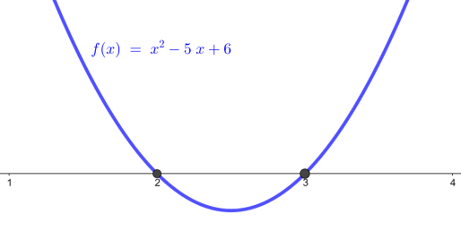
\includegraphics[width=\textwidth]{../Mathematik_1/Bilder/ungleichungen_quadratische_funktion_nullstellen.png}
\end{minipage}
\begin{minipage}{0.55\textwidth}
\begin{itemize}
\item Gezeigt ist der Graph der Funktion
\(
	f(x)=x^2-5x+6.
	\)
\item Positive Funktionswerte treten links der kleineren und rechts der gr��eren Nullstelle auf. Genau diese Bereiche bilden die zuvor berechnete L�sungsmenge.
\end{itemize}
\end{minipage}
\end{exabox}

\noindent\textbf{Bemerkungen:}
\begin{itemize}
\item Die L�sungsmenge l�sst sich damit sowohl rechnerisch als auch am Graphen erkennen.
\item Quadratische Terme lassen sich mithilfe ihrer Nullstellen faktorisieren:
\(
	ax^2+bx+c=a(x-x_1)(x-x_2).
	\)
\item Das Grundprinzip aus Nullstellenbestimmung und Vorzeichenanalyse bleibt auch bei polynomialen Ungleichungen h�herer Ordnung erhalten.
\end{itemize}

Bei einer \textbf{Bruchungleichung} kommt eine weitere Schwierigkeit hinzu: Das Vorzeichen eines Bruches h�ngt sowohl vom Z�hler als auch vom Nenner ab. Gleichzeitig darf der Nenner niemals Null werden. Eine Multiplikation mit dem Nenner ist deshalb erst dann m�glich, wenn bekannt ist, welches Vorzeichen dieser besitzt.

Besonders einfach ist der Fall, dass der Bruch mit Null verglichen wird. Ein Bruch ist nichtnegativ, wenn Z�hler und Nenner dasselbe Vorzeichen besitzen oder der Z�hler Null ist.

\begin{exabox}{L�sen einer Bruchungleichung mit rechter Seite Null}{ }
Betrachtet wird

$$
\frac{2x-1}{x+4}\geq0.
$$

Der Nenner darf nicht verschwinden, also gilt zun�chst

$$
x\neq-4.
$$

Damit der Bruch nichtnegativ ist, m�ssen Z�hler und Nenner gleiches Vorzeichen besitzen:

$$
\begin{array}{rcl}
\dfrac{2x-1}{x+4}\geq0
&\Leftrightarrow&
\begin{cases}
2x-1\geq0 \land x+4>0,\\
2x-1\leq0 \land x+4<0
\end{cases}
\\[2ex]
&\Leftrightarrow&
\begin{cases}
x\geq\dfrac12 \land x>-4,\\
x\leq\dfrac12 \land x<-4
\end{cases}
\\[2ex]
&\Leftrightarrow&
\begin{cases}
x\geq\dfrac12,\\
x<-4.
\end{cases}
\end{array}
$$

Die beiden F�lle werden vereinigt. Damit ergibt sich

$$
x\in(-\infty,-4)\cup\left[\frac12,\infty\right).
$$

\end{exabox}

Steht auf der rechten Seite dagegen eine von Null verschiedene Zahl, kann nicht allein das Vorzeichen des gesamten Bruches betrachtet werden. Um den Nenner zu beseitigen, m�sste mit \(x+4\) multipliziert werden. Dabei h�ngt die Richtung des Ungleichheitszeichens davon ab, ob \(x+4\) positiv oder negativ ist. Deshalb wird \textbf{zuerst das Vorzeichen des Nenners unterschieden}.

\begin{exabox}{L�sen einer Bruchungleichung mit konstanter rechter Seite}{ }
Betrachtet wird

$$
\frac{2x-1}{x+4}\geq3.
$$

Der Nenner verschwindet f�r \(x=-4\). Dieser Wert geh�rt nicht zum Definitionsbereich. F�r alle �brigen Werte werden zwei F�lle unterschieden.

$$
\begin{array}{rcll}
\dfrac{2x-1}{x+4}\geq3
&\Leftrightarrow&
\begin{cases}
x+4>0 \land 2x-1\geq3(x+4),\\
x+4<0 \land 2x-1\leq3(x+4)
\end{cases}
& \text{Nenner-Vorzeichen}
\\[3ex]
&\Leftrightarrow&
\begin{cases}
x>-4 \land x\leq-13,\\
x<-4 \land x\geq-13
\end{cases}
& \text{Ungleichungen l�sen}
\\[3ex]
&\Leftrightarrow&
\begin{cases}
x\in\emptyset,\\
x\in[-13,-4)
\end{cases}
& \text{F�lle auswerten}
\\[3ex]
&\Leftrightarrow&
x\in[-13,-4).
& \text{vereinigen}
\end{array}
$$

Im ersten Fall widersprechen sich die Bedingungen \(x>-4\) und \(x\leq-13\); dieser Fall liefert daher keine L�sung. Im zweiten Fall m�ssen \(x<-4\) und \(x\geq-13\) gleichzeitig erf�llt sein. Daraus entsteht das Intervall \([-13,-4)\).
\end{exabox}

Bei einer \textbf{Betragsungleichung} entsteht die Fallunterscheidung aus der Definition des Betrags. Der Betrag eines Ausdrucks h�ngt davon ab, ob dieser Ausdruck nichtnegativ oder negativ ist:

$$
|T|=
\begin{cases}
T,&T\geq0,\\
-T,&T<0.
\end{cases}
$$

F�r die Ungleichung \(|x-7|<5\) wird deshalb das Vorzeichen von \(x-7\) unterschieden.

\begin{exabox}{L�sen einer Betragsungleichung}{ }

$$
\begin{array}{rcl}
|x-7|<5
&\Leftrightarrow&
\begin{cases}
x-7\geq0 \land x-7<5,\\
x-7<0 \land -(x-7)<5
\end{cases}
\\[2ex]
&\Leftrightarrow&
\begin{cases}
x\geq7 \land x<12,\\
x<7 \land x>2
\end{cases}
\\[2ex]
&\Leftrightarrow&
\begin{cases}
x\in[7,12),\\
x\in(2,7)
\end{cases}
\\[2ex]
&\Leftrightarrow&
x\in(2,12).
\end{array}
$$

\end{exabox}

Bei einfachen Betragsungleichungen l�sst sich dasselbe Ergebnis auch unmittelbar aus der Bedeutung des Betrags ablesen:

$$
|x-7|<5
\;\Leftrightarrow\;
-5<x-7<5
\;\Leftrightarrow\;
2<x<12.
$$

Die ausf�hrliche Fallunterscheidung bleibt dennoch wichtig, da sie auch dann funktioniert, wenn kompliziertere Ausdr�cke innerhalb des Betrags auftreten.

Treten mehrere dieser Strukturen gleichzeitig auf, m�ssen die notwendigen Fallunterscheidungen miteinander kombiniert werden. Bei einem Betrag im Z�hler und einem variablen Nenner muss beispielsweise sowohl das Vorzeichen des Nenners als auch das Vorzeichen des Ausdrucks innerhalb des Betrags ber�cksichtigt werden.
  % �quivalenzumformungen

\chapter{Funktionen}
\etocsettocstyle{\section*{Inhalt dieses Kapitels}}{}
\section*{Leitidee}

Funktionen sind das zentrale Objekt der Analysis: Sie beschreiben, wie Gr��en voneinander abh�ngen, und erm�glichen es dadurch, mathematische Zusammenh�nge und reale Prozesse zu modellieren. Dabei kann eine Funktion auf unterschiedliche Weise betrachtet werden -- durch ihre Funktionsgleichung, ihren Graphen oder durch charakteristische Eigenschaften wie Nullstellen, Monotonie und Symmetrie.

Ausgehend vom allgemeinen \textbf{Funktionsbegriff} werden zun�chst grundlegende \textbf{Eigenschaften von Funktionen} untersucht. Anschlie�end stehen wichtige Funktionsklassen im Mittelpunkt: lineare Funktionen, Potenz- und Wurzelfunktionen, Polynome, rationale Funktionen, Exponential- und Logarithmusfunktionen sowie trigonometrische Funktionen. Jede dieser Funktionsklassen besitzt typische Eigenschaften und eignet sich zur Beschreibung bestimmter mathematischer Zusammenh�nge.

Ein weiterer Schwerpunkt liegt auf dem L�sen von \textbf{Gleichungen}, die aus diesen Funktionen entstehen. Dabei wird deutlich, wie die algebraischen Methoden aus dem vorherigen Kapitel mit der Untersuchung von Funktionen zusammenwirken.

Schlie�lich k�nnen Funktionen miteinander \textbf{verkn�pft und komponiert} werden. Auf diese Weise entstehen aus elementaren Funktionen komplexere Modelle, mit denen sich beispielsweise Wachstumsprozesse oder Schwingungen mathematisch beschreiben lassen.



  % Leitidee Funktionen

\bigskip
\localtableofcontents
\newpage

\setcounter{satz}{0} \setcounter{def}{0} \setcounter{exa}{0}  \section{Funktionen}\label{MA1-funktionen}

\begin{table}[H]
  \centering
  \begin{tabularx}{\textwidth}{p{0.9\textwidth} p{0.1\textwidth}}
    \toprule
	  \multicolumn{2}{c}{\textbf{�bersicht �ber Lernziele und Voraussetzungen}}\\
    \midrule
	  \textbf{Lernziele} &\\[.5\normalbaselineskip]
\tabitem Funktionen als eindeutige Zuordnungen pr�zise beschreiben &\\
\tabitem Definitionsbereich, Zielmenge und Bildmenge unterscheiden und bestimmen &\\
\tabitem Funktionen in mathematischer Formelsprache darstellen und interpretieren &\\
\tabitem Funktionsgraphen als Mengen geordneter Paare interpretieren &\\
\tabitem Funktionen von allgemeineren Relationen unterscheiden &\\
    \midrule
	  \textbf{Voraussetzungen} \\[.5\normalbaselineskip]
	  \tabitem Mengenoperationen und Intervallschreibweisen & \abschnittsverweis{MA1-mengen-und-logik}\\
	  \tabitem Grundrechenarten & \abschnittsverweis{MA1-zahlenmengen}\\
	  \tabitem �quivalenzumformungen & \abschnittsverweis{MA1-aequivalenzumformungen}\\
    \bottomrule
  \end{tabularx}
\end{table}

\ifintegriereaufgaben \noindent �bungsaufgaben zum Thema finden Sie hier: \hyperref[MA1-funktionen-aufgaben]{Aufgaben}
\vspace{0.3cm}
\hrule
\fi

\subsection{Was ist eine Funktion?}

Eine \textbf{Abbildung} (\emph{mapping}) namens $f$ ordnet jedem Element $x$ eines Definitionsbereichs $D$ (\emph{domain}) genau ein Element $y$ einer Zielmenge  $Z$ (\emph{codomain}) zu. In mathematischer Kurzschreibweise sieht das so aus:
	\[ f: D \to Z, x\mapsto y\,.\]
	Dieser Ausdruck sagt aber noch nichts dar�ber, wie die Abbildung im Detail funktioniert. Was fehlt ist die Zuordnungsvorschrift oder Abbildungsvorschrift. Anstatt eine "\,Gleichung $y=f(x)$"\, wie in der Schule anzugeben, f�hren wir einen Abbildungspfeil ein: 
	\[  x\mapsto f(x)\,.\]
	Da der Definitionsbereich, die Zielmenge und die Abbildungsvorschrift zusammen eine Abbildung so definieren, dass man in der Lage ist die Abbildung zu untersuchen, fasst man diese Informationen typischerweise zusammen und gibt eine Abbildung in der folgenden Form an:  
\begin{defbox}{Abbildung von \(D\) nach \(Z\) mit Abbildungsvorschrift}{ }
	$ f: D\to Z, x\mapsto f(x)\,.$
\end{defbox}
\noindent{\textbf{ Bemerkungen:}}
\begin{itemize}
	\item Statt $f(x)$ wird typischerweise eine Formel angegeben, beispielsweise $ x\mapsto \sin(x)$ oder \( x\mapsto 10\cdot x^3-2\cdot\sqrt{x}\).
	\item Wenn der Definitionsbereich und die Zielmenge fixierte Mengen von Zahlen, von geometrischen Objekten oder von Funktionen (!) \dots  sind, nennt man eine Abbildung meist eine Funktion (\emph{function}). Mathematisch sind Abbildungen und Funktionen dasselbe. 
\end{itemize}

Es gibt mehrere Vorstellungen von Abbildungen (Funktionen). Hier sind vier davon. 

\begin{exabox}{Funktion als Maschine}{ }
\begin{minipage}{0.3\textwidth}
	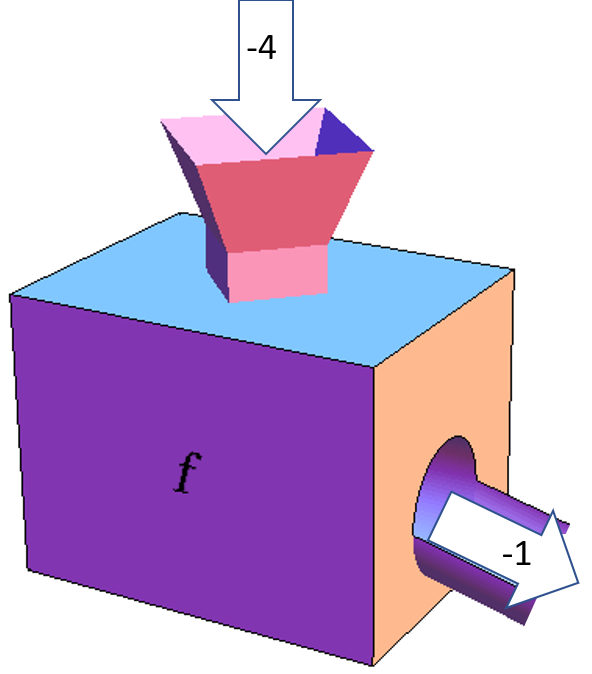
\includegraphics[width=\textwidth]{../Mathematik_1/Bilder/funktionen_maschinenmodell_zahlenwerte.png} 
\end{minipage}
\begin{minipage}{0.7\textwidth}
Eine Abbildung $f$ ist eine Maschine, in die man ein Teil aus einer Menge $D$ als Rohmaterial hineinwerfen kann und aus der man dann ein Teil aus $Z$ als Produkt zur�ckerh�lt:
\begin{itemize}
	\item Alle Teile aus $D$ m�ssen akzeptiert werden.
	\item Nur Teile aus $Z$ d�rfen produziert werden. 
	\item Es wird immer genau ein Teil produziert (nicht null, nicht sieben). 
	\item Wenn man dasselbe Teil aus $D$ nochmal hinein wirft, muss wieder dasselbe Teil aus $Z$ produziert werden wie beim ersten Mal. 
\end{itemize}
\end{minipage}
\end{exabox}

\begin{exabox}{Funktion als Tabelle}{ }
\begin{minipage}{0.2\textwidth}
	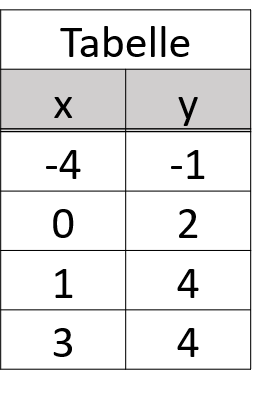
\includegraphics[width=\textwidth]{../Mathematik_1/Bilder/funktionen_darstellung_wertetabelle.png} 
\end{minipage}
\begin{minipage}{0.7\textwidth}
Eine Abbildung $f$ ist eine Tabelle (ggf unendlich lang), aus der man f�r jedes $x\in D$ das zugeh�rige $f(x) \in Z$ ablesen kann:
\begin{itemize}
	\item In der $x$-Spalte der Tabelle muss jedes Element aus $D$ genau einmal vorkommen (nicht null mal, nicht sieben mal). 
	\item In der $y$-Spalte der Tabelle d�rfen nur Elemente aus $Z$ stehen. 
	\item In dem Beispiel ist $Z=\mathbb Z$. 
	\item Die Reihenfolge der Zeilen in der Tabelle ist egal. 
\end{itemize}
\end{minipage}
\end{exabox}

\begin{exabox}{Funktion als Pfeildiagramm}{ }
\begin{minipage}{0.3\textwidth}
	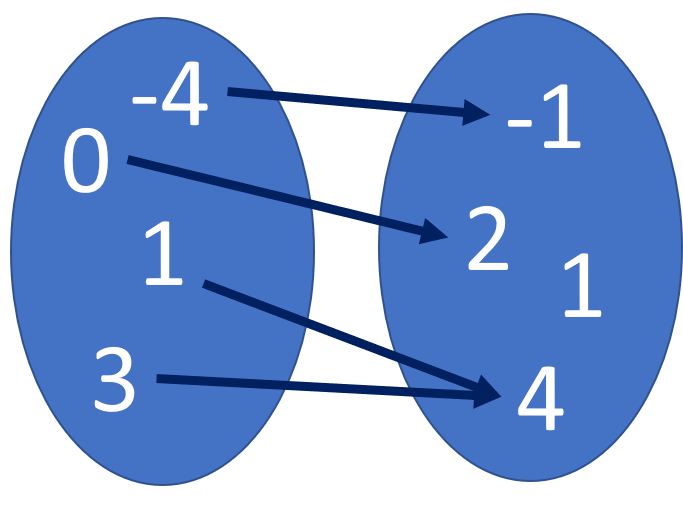
\includegraphics[width=\textwidth]{../Mathematik_1/Bilder/funktionen_darstellung_pfeildiagramm.png} 
\end{minipage}
\begin{minipage}{0.7\textwidth}
\begin{itemize}
	\item Von jedem Element in $D$ muss genau ein Pfeil starten und zu einem Element in $Z$ f�hren. 
	\item Es ist erlaubt, dass mehrere Pfeile auf einem Element von $Z$ enden. 
	\item Es ist auch erlaubt, dass Elemente von $Z$ von keinem Pfeil erreicht werden. 
\end{itemize}
\end{minipage}
\end{exabox}

\begin{exabox}{Funktion als Graph}{ }
\begin{minipage}{0.3\textwidth}
	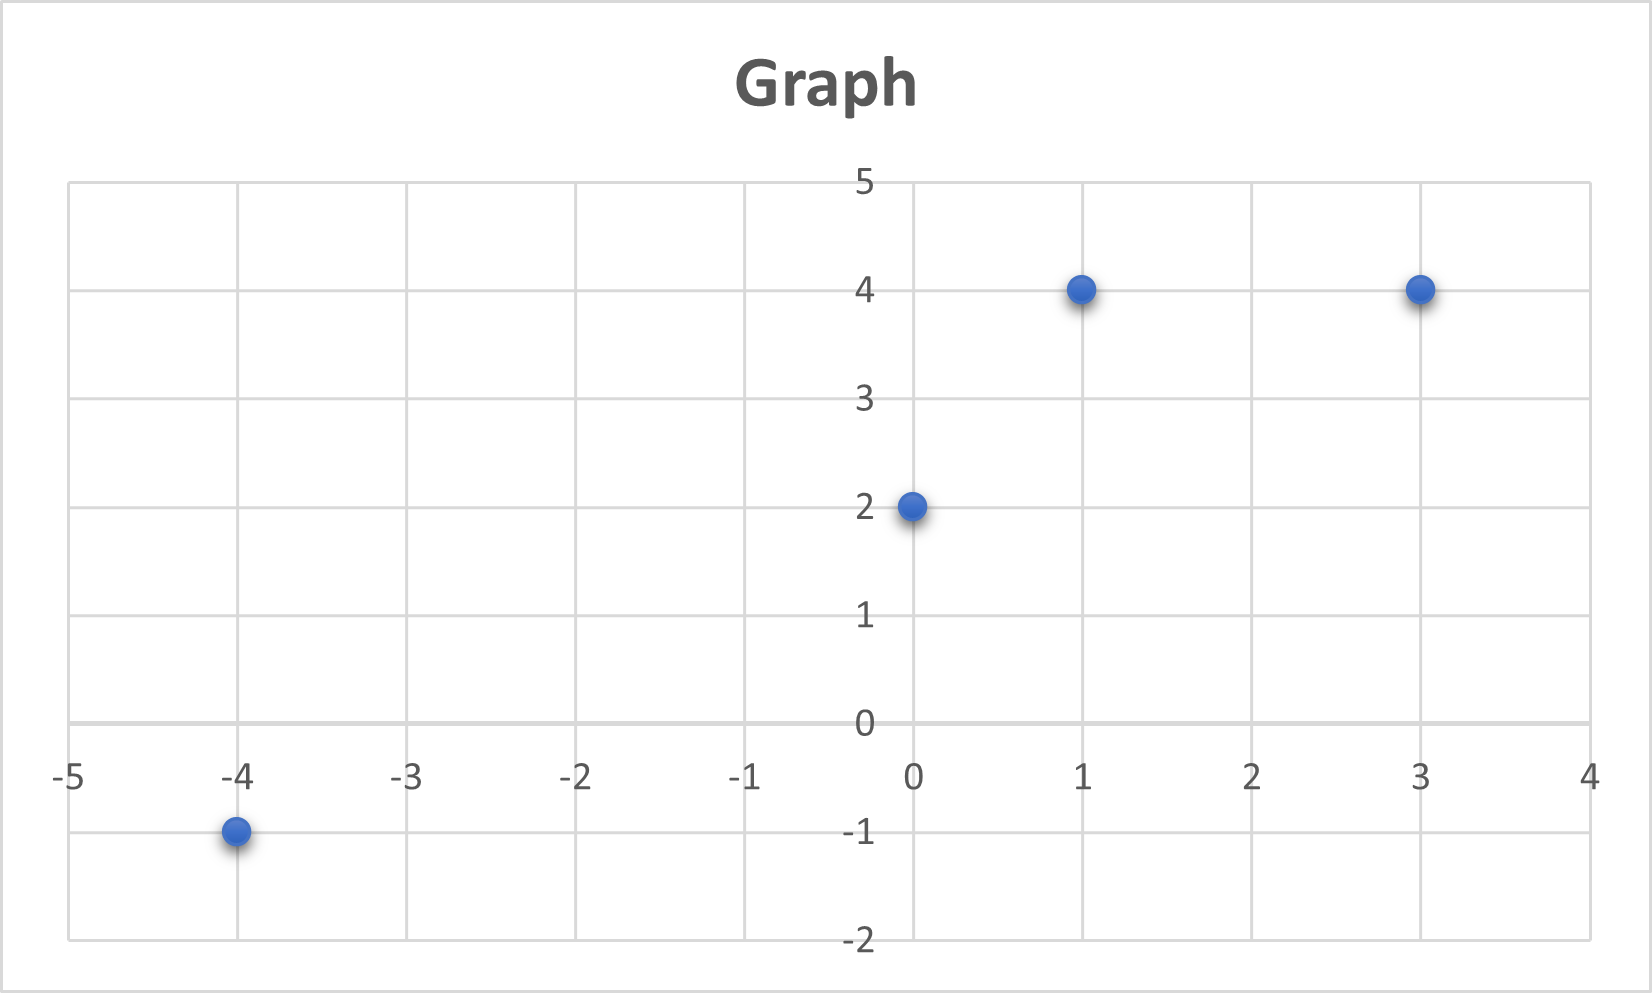
\includegraphics[width=\textwidth]{../Mathematik_1/Bilder/funktionen_darstellung_diskreter_graph.png} 
\end{minipage}
\begin{minipage}{0.7\textwidth}
 Hier ist von Funktionen die Rede, die man in einem Diagramm aufmalen kann. 
\begin{itemize}
	 \item $D$ und $Z$ sind also Mengen von Zahlen. 
	 \item Der Definitionsbereich \(D\) wird auf der \(x\)-Achse dargestellt, die Zielmenge \(Z\) auf der \(y\)-Achse.
	 \item $D$ und $Z$ k�nnen sich nat�rlich auch jeweils �ber die gesamten Achsen erstrecken. 
	 \item Zu jedem $x\in D$ (und nur f�r solche $x$ ) ist genau ein $y\in Z$ markiert. 
 \end{itemize}
\end{minipage}
\end{exabox}

  
\subsection{Definitions- und Bildbereich}

Der \textbf{Definitionsbereich} ist die Menge aller mathematischen Objekte, die in eine Funktion hineingegeben werden d�rfen. In der Pfeilvorstellung einer Funktion bildet der Definitionsbereich den Startpunkt der Pfeile; die Pfeilspitzen liegen in der \textbf{Zielmenge}. 

Diese Vorstellung findet sich unmittelbar in der mathematischen Schreibweise

$$
f:D\to Z,\qquad x\mapsto f(x)
$$

wieder: Ein Element \(x\in D\) am Pfeilanfang wird auf ein Element \(f(x)\in Z\) an der Pfeilspitze abgebildet.

Definitionsbereich \(D\) und Zielmenge \(Z\) sind h�ufig Teilmengen der reellen Zahlen -- oder sogar ganz \(\mathbb R\). Im folgenden Beispiel muss der Definitionsbereich $D \subsetneq \mathbb R$ eingeschr�nkt werden, weil die Funktion an der Stelle $x=3$ nicht definiert ist:\marginpar{Aufgabe}
\begin{exabox}{Funktion mit $D \subsetneq \mathbb R$}{ }
  $f: D \to \mathbb R, \; x\mapsto \displaystyle{\frac{x^2+7}{x-3}} \Rightarrow D = \mathbb R\setminus \{3\}\,.$
\end{exabox}

Hinter den meisten �blichen Operationen mit Zahlen stecken Funktionen - auch wenn sie oft nicht explizit als solche bezeichnet werden: 
\begin{itemize}
  \item Addition reeller Zahlen: $ +:\, \mathbb R^2 \to \mathbb R,\; (x,y) \mapsto x+y\,,$ 
  \item Division reeller Zahlen: $ /:\, \{(x,y)\in \mathbb R^2: y \not = 0\} \to \mathbb R,\; (x,y) \mapsto \displaystyle{\frac{x}{y}}\,,$
  \item Fakult�t: $!:\, \mathbb N_0 \to \mathbb N^+,\; n \mapsto n\cdot(n-1)\cdot(n-2)\cdot \dots \cdot 2\cdot 1 =: n!\,,$ 
  \item Binomialkoeffizient: $ \displaystyle{{\cdot}\choose{\cdot}}:\, \big\{ (n,k)\in\mathbb N_0^2: k\leq n\big\} \to \mathbb N_0,\; (n,k) \mapsto \displaystyle{ \frac{n!}{k!\cdot (n-k)!} }\,.$ 
\end{itemize}


 
Die Menge der tats�chlich angenommenen Funktionswerte hei�t \textbf{Bild}, \textbf{Bildbereich} oder \textbf{Bildmenge}\marginpar{\small{Aufgabe}} (\emph{image}) und wird mit \(f(D)\) bezeichnet. Dabei gilt

$$
f(D)\subseteq Z.
$$

Die Bildmenge kann also kleiner als die Zielmenge sein, sie kann aber auch mit der Zielmenge �bereinstimmen.

Die Menge $S$, die in einem der folgenden Beispiele auftaucht, bezeichne die Menge aller endlichen Zeichenketten.

\begin{exabox}{Unterschiedliche Bildmengen}{ }
\begin{itemize}
  \item $f_1: [3,4] \to \mathbb R,\; x\mapsto x^2 \; \Rightarrow \; f_1(D) = [9,16]$. 

\item   $f_2:S \to S, \; x\mapsto \displaystyle{\begin{cases} \verb-a-, \quad x=\verb-b- \\  x, \quad x\not=\verb-b- \end{cases}} \Rightarrow \; f_2(D) = S\setminus \{ \verb-b-\}$.

\item $f_3: \mathbb R \to \mathbb R^2,\; t \mapsto \left(\cos(2\pi t), \sin(2\pi t)\right) \; \Rightarrow \; f_3(D) = \left\{(x,y)\in \mathbb R^2:  x^2 + y^2 = 1\right\}\,.$

\item $f_4: \mathbb R \to \mathbb R^2,\; t\mapsto \left(e^t \cdot \cos(2 \pi\cdot t), e^t \cdot \sin(2 \pi\cdot t)\right)$ Die Bildmenge bildet geometrisch eine logarithmische Spirale.  \end{itemize}
\end{exabox}

Die folgende Skizze veranschaulicht den Definitionsbereich $D$, die Zielmenge $Z$ und die Bildmenge $f(D)$ einer Funktion $f$.

\begin{center}
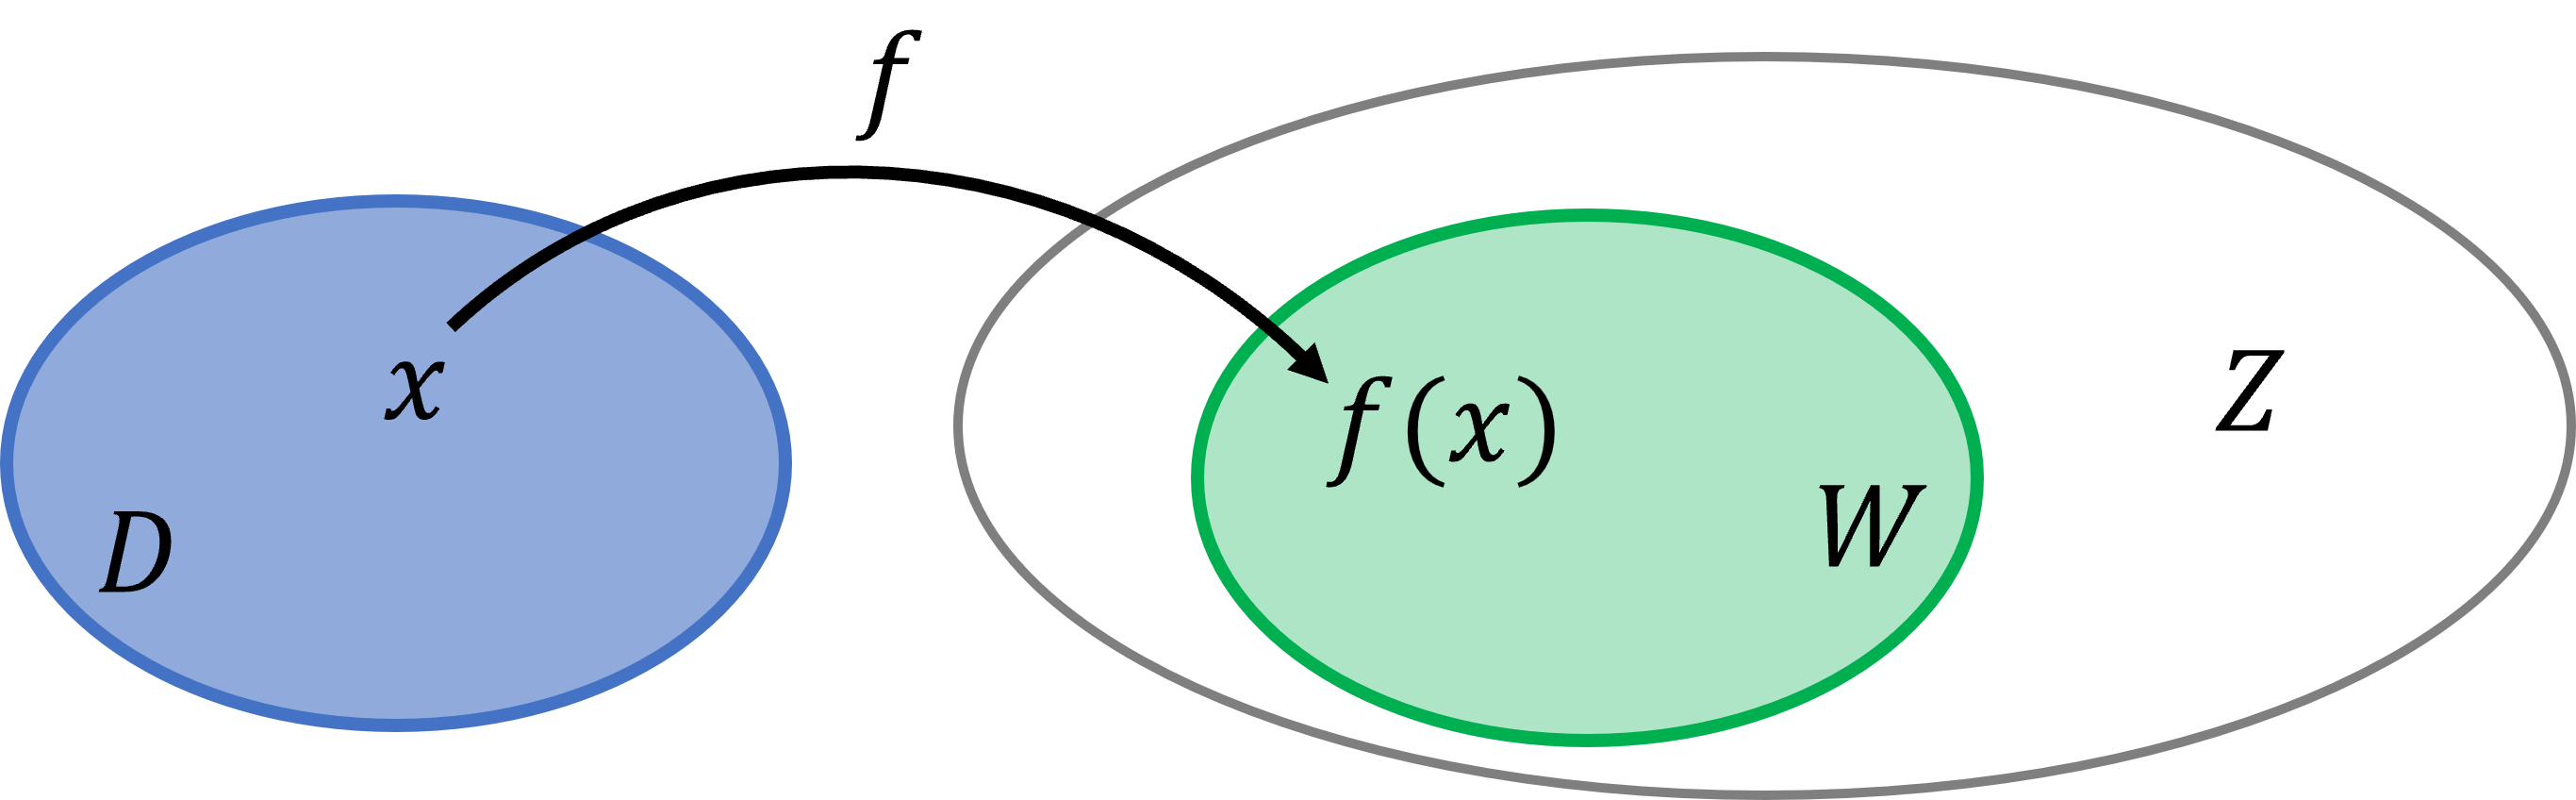
\includegraphics[width=0.8\textwidth]{../Mathematik_1/Bilder/funktionen_definitionsbereich_zielmenge_bildmenge.png}
\end{center}

\noindent{\textbf{ Bemerkungen:}}
\begin{itemize}
	\item Der Name der Funktion ist $f$. Der Ausdruck $f(x)$ bezeichnet den Funktionswert von \(f\) an der Stelle \(x\) und ist ein Element der Zielmenge $Z$. 
	\item Fiese (pathologische) Funktionen bilden keine anschaulichen Graphen. Die Dirichlet Funktion ist eine von ihnen: 
  $$ f: \mathbb R \to \{0, 1\}, \quad x\mapsto \begin{cases} 1,\quad x\in \mathbb Q, \\ 0,\quad x\in \mathbb R\setminus{\mathbb Q}\,.\end{cases} $$
  \item Eine Funktion braucht nicht unbedingt eine ausdr�ckliche Abbildungsvorschrift wie $x \mapsto \sin(x^{2})$ zu haben. Eine Abbildung kann auch in Worten beschrieben werden, beispielsweise
	  \begin{center}
  "Nimm den dritten Buchstaben von $x$, falls vorhanden, ansonsten $*$." 
  \end{center}
  Oder sie ist nur indirekt gegeben, zum Beispiel als Stammfunktion:
  \begin{center}
  "$F$ ist die Stammfunktion von $x\mapsto e^{-x}$ f�r $F(0)=0$."
  \end{center}
\item Beim Programmieren kommen ebenfalls sogenannte Funktionen vor. Der Funktionsbegriff in Programmiersprachen ist jedoch allgemeiner als der mathematische Funktionsbegriff; beispielsweise k�nnen Programmfunktionen ohne explizite Eingabe aufgerufen werden.	
\end{itemize}

\subsection{Funktionsgraphen und Relationen}

F�r eine Funktion

$$
f:D\to Z
$$

kann jede Zuordnung \(x\mapsto f(x)\) als geordnetes Paar

$$
(x,f(x))\in D\times Z
$$

aufgefasst werden. Der \textbf{Graph einer Funktion} ist die Menge all dieser Paare:

$$
G_f
=
\{(x,f(x)):x\in D\}
\subseteq D\times Z.
$$

Die formale Schreibweise f�r den Graphen $G_f$ bedeutet: F�r jedes \(x\) aus dem Definitionsbereich wird das geordnete Paar aus \(x\) und dem zugeh�rigen Funktionswert \(f(x)\) in den Graphen aufgenommen.

F�r eine reelle Funktion \(f:D\to\mathbb R\) mit \(D\subseteq\mathbb R\) gilt insbesondere

$$
G_f\subseteq\mathbb R^2.
$$

Deshalb l�sst sich der Funktionsgraph als Menge von Punkten in der Ebene darstellen.

Allerdings ist nicht jede Teilmenge von \(\mathbb R^2\) der Graph einer Funktion. Die Kreislinie liefert daf�r ein anschauliches Beispiel.

%\subsection{Geordnete Tupel}
%
%Wenn man ein Gef�hl f�r den Funktionsverlauf einer Funktion \(f: \mathbb R \to \mathbb R,\, x\mapsto f(x)\) bekommen m�chte, dann geht man oft wie folgt vor 
%\begin{enumerate}
%	\item man w�hlt eine paar Werte f�r \(x \in \mathbb R\): das sind die St�tzstellen \(x_i, \, i=1,2,3,\cdots\)
%	\item man berechnet die zu den St�tzstellen geh�rigen Funktionswerte \(y_i = f(x_i) \in \mathbb R\)
%	\item man zeichnet in ein zwei-dimensionales Koordinatensystem die Punkte \(P_i = (x_i|y_i)\) 
%	\item man verbindet die Punkte miteinander und behauptet, dass die Funktion so aussieht!\footnote{Falls die Funktion stetig ist, ist das ein guter Ansatz!}
%\end{enumerate} 
%
%Die Punkte \(P(x|y)\), die zu \(f\) geh�ren sind Tupel und das hei�t, dass die Reihenfolge der Koordinaten fixiert ist und eine Rolle spielt: erst \(x\) dann \(y\). 

\begin{exabox}{Funktionsgraph oder nicht?}{ }
\begin{minipage}{0.3\textwidth}
	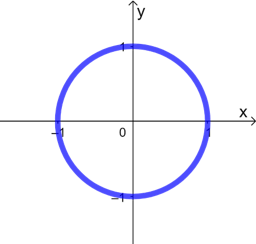
\includegraphics[width=\textwidth]{../Mathematik_1/Bilder/relationen_einheitskreis.png} 
\end{minipage}
\begin{minipage}{0.7\textwidth}
\begin{itemize}
	\item Ist die Kreislinie der Graph einer Funktion? 
	\item Wie l��t sich die Kreislinie beschreiben? 
\end{itemize}
\end{minipage}
\end{exabox}

Die Figur links, die Kreislinie, ist nicht der Graph einer Funktion, denn zu fast jedem \(x \in (-1,1) \) m�ssten zwei verschiedene Funktionswerte zugeordnet werden!\footnote{Die Kreislinie ist eine sogenannte Relation. Eine Relation ist etwas allgemeineres als eine Funktion.}

\subsection{Was ist eine Relation?}

Eine \textbf{Relation} beschreibt, welche Elemente mehrerer Mengen miteinander in Beziehung stehen. Formal ist eine beliebige Teilmenge eines \underline{kartesischen Produkts}\randverweis{MA1-mengen-und-logik}

$$
A_1\times A_2\times\cdots\times A_n
$$

eine \textbf{\(n\)-stellige Relation}.

Eine zweistellige Relation besteht damit aus geordneten Paaren, eine dreistellige Relation aus geordneten Tripeln usw.

\begin{exabox}{Relationen}{ }
  \begin{itemize}
    \item $\{ (1,2), (3,4), (1,5)\} \subseteq \mathbb N_0 \times \mathbb N_0$ 
    \item $\left\{ \left(\mathrm{Anton}, \mathrm{Weber}, 293\right), \left(\mathrm{Bea}, \mathrm{Knorr}, 298\right), \left(\mathrm{Lisa}, \mathrm{Kann}, 284\right) \right\} \subseteq S\times S\times \mathbb N_0$
  \end{itemize}
\end{exabox}

Das zweite Beispiel l�sst die wesentliche Bedeutung von Relationen in der Informatik erahnen: sie dienen als Datenspeicher.

Es gibt mehrere �bliche Vorstellungen von Relationen. Hier sind drei davon. 

\begin{enumerate}
  \item {\textbf{Tabelle:}} Fast alle aktuell �blichen  Datenbanksysteme verwalten Tabellen. Mathematische Relationen sind nichts anderes als Tabellen mit  ein  paar  Besonderheiten.  Deshalb  hei�en  diese  Datenbanksysteme auch relational.

\begin{center}
  \begin{tabular}{c|c|c}
    Vorname & Nachname & Matrikelnummer \\
    \hline
  Bea & Knorr & $298$ \\
  Lisa & Kann & $284$ \\
  Anton & Weber & $293$
  \end{tabular}
\end{center}

\begin{itemize}
  \item In jeder Spalte der Tabelle d�rfen nur Eintr�ge aus der jeweiligen Menge des kartesischen Produkts stehen. 
  \item Die Reihenfolge der Zeilen ist egal. 
  \item Keine Zeile darf als Ganzes doppelt vorkommen; Teile der Zeile d�rfen sich aber wiederholen. 
\end{itemize}
      
Bei Abbildungen bzw. Funktionen gibt es im Unterschied zur Relation nur zwei Spalten. Au�erdem \textbf{muss} in der linken Spalte jedes Elemente des Definitionsbereichs vorkommen - und das \textbf{genau einmal}. %Frage


\item {\textbf{Liniendiagramm:}}
  \begin{itemize}
    \item Elemente  der  Mengen  aus  dem  Produkt  sind  durch  Linien  verbunden.  
    \item Jede Linie geht durch genau ein Element aus jeder Menge des kartesischen Produkts. 
    \item Linien d�rfen teilweise �bereinander liegen. 
    \item Keine zwei beliebige Linien d�rfen aber komplett �bereinstimmen. 
  \end{itemize}

Bei Abbildungen bzw. Funktionen malt man typischerweise Pfeile statt Linien. Au�erdem sind nur zwei Mengen beteiligt und es muss von jedem Element des Definitionsbereichs genau ein Pfeil ausgehen. 


\item {\textbf{Geometrische Objekte im $\mathbb R^n$:}}

Eine $n$-stellige Relation zwischen reellen Zahlen ist eine Teilmenge des $\mathbb R^n$, also eine Menge von Punkten. Umgekehrt ist jedes auch noch so komische geometrische Objekt eine Relation! 

\begin{exabox}{Relationen}{ }
  \begin{itemize}
    \item die Kreislinie: $P:=\left\{ (x,y)\in \mathbb R^2: x^2+y^2 = 1\right\}$.
	  \item die �Gr��er-Gleich�-Relation: $\geq := \left\{ (x,y)\in \mathbb R^2: x\geq y \right\}$,
\end{itemize}
	\centering
	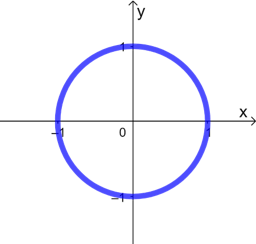
\includegraphics[width=0.4\textwidth]{../Mathematik_1/Bilder/relationen_einheitskreis.png} \hspace{2cm}
	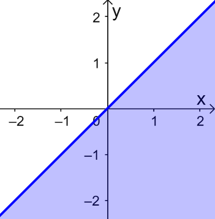
\includegraphics[width=0.4\textwidth]{../Mathematik_1/Bilder/relationen_halbebene_y_kleiner_gleich_x.png}
\end{exabox}

Bei einem Funktionsgraph muss jedem $x$ aus dem Definitionsbereich genau ein $y$ (nicht null, nicht zwei oder mehr) aus der Bildmenge zugeordnet werden, diese Einschr�nkung gilt nicht f�r Relationen.
\end{enumerate}


Eine Funktion ist damit eine besondere zweistellige Relation. F�r eine Funktion $ f:D\to Z $ muss zu jedem \(x\in D\) genau ein \(y\in Z\) geh�ren. Eine allgemeine Relation besitzt diese Einschr�nkung nicht: Zu einem \(x\) k�nnen kein, genau ein oder mehrere \(y\)-Werte geh�ren.

Der Funktionsgraph $ G_f=\{(x,f(x)):x\in D\} $ ist daher eine Relation mit einer zus�tzlichen Eindeutigkeitsbedingung.
  % Definition Funktion
\newpage
\setcounter{satz}{0} \setcounter{def}{0} \setcounter{exa}{0}  \section{Eigenschaften von Funktionen}\label{MA1-eigenschaften-von-funktionen}

\begin{table}[H]
  \centering
  \begin{tabularx}{\textwidth}{p{0.9\textwidth} p{0.1\textwidth}}
    \toprule
	  \multicolumn{2}{c}{\textbf{�bersicht �ber Lernziele und Voraussetzungen}}\\
    \midrule
	  \textbf{Lernziele} &\\[.5\normalbaselineskip]
    \tabitem Nullstellen einer Funktion bestimmen &\\
    \tabitem das asymptotische Verhalten einer Funktion qualitativ angeben &\\
    \tabitem Monotonie und Symmetrie pr�fen &\\
    \tabitem Periodizit�t pr�fen &\\
    \tabitem Injektivit�t, Surjektivit�t und Bijektivit�t unterscheiden &\\
    \tabitem die Umkehrbarkeit einer Funktion bestimmen &\\
    \tabitem die genannten Eigenschaften zur Erstellung eines Funktionsgraphen einsetzen &\\[.5\normalbaselineskip]
    \midrule
	  \textbf{Voraussetzungen} \\[.5\normalbaselineskip]
	  \tabitem Grundrechenarten & \abschnittsverweis{MA1-zahlenmengen}\\
	  \tabitem �quivalenzumformungen & \abschnittsverweis{MA1-aequivalenzumformungen}\\
	  \tabitem Definition einer Funktion & \abschnittsverweis{MA1-funktionen}\\
    \bottomrule
  \end{tabularx}
\end{table}

\ifintegriereaufgaben \noindent �bungsaufgaben zum Thema finden Sie hier: \hyperref[MA1-eigenschaften-von-funktionen-aufgaben]{Aufgaben}
\vspace{0.3cm}
\hrule
\fi

\subsection{Nullstellen, Asymptotik, Symmetrie und Periodizit�t }

Funktionen treten in sehr unterschiedlichen Anwendungen auf: bei wirtschaftlichen Machbarkeitsanalysen, bei der Untersuchung der Effizienz technischer Anlagen oder bei der Auswertung von Daten. In allen diesen Situationen geht es darum, Abh�ngigkeiten zwischen Gr��en zu erkennen, mathematisch zu beschreiben und zu interpretieren.

Dabei ist nicht immer eine vollst�ndige Berechnung notwendig. H�ufig liefern bereits einige charakteristische Eigenschaften einer Funktion wichtige Informationen �ber ihr Verhalten. Dazu geh�ren beispielsweise Nullstellen, Symmetrien, Periodizit�t, Monotonie und das Verhalten f�r betragsm��ig gro�e Werte der Variablen.

Eine Funktion \(f:D\to Z\) kann solche Eigenschaften auf ihrem gesamten Definitionsbereich oder nur auf bestimmten Teilbereichen besitzen. Die Symmetrie eines Funktionsgraphen ist beispielsweise eine globale Eigenschaft, w�hrend Monotonie auch auf einzelnen Intervallen untersucht werden kann.

\begin{defbox}{Eigenschaften}{ } 
	\begin{itemize}
		\item \textbf{Nullstellen} sind diejenigen \(x\in D\), deren zugeordneter Funktionswert null ist. 
		\item \textbf{Asymptotisches Verhalten} ist das Verhalten der Funktionswerte f�r betragsm��ig gro�e Werte von \(x\). %Im Allgemeinen beschreibt das Verhalten der Funktionswerte, wenn sich \(x\) bestimmten Grenzwerten n�hert, beispielsweise \(x\to\infty\), \(x\to-\infty\) oder einer Stelle, an der die Funktion nicht definiert ist.	
		\item \textbf{Punktsymmetrie} liegt vor, wenn der Graph von \(f\) am Koordinatenursprung \( \left( 0|0\right)\) gespiegelt erscheint.
		\item \textbf{Achsensymmetrie} liegt vor, wenn der Graph von \(f\) an der \(y\)-Achse gespiegelt erscheint.
		\item \textbf{Periodizit�t} liegt vor, wenn sich die Funktionswerte von \(f\) in einem festen Abstand wiederholen.
		\item \textbf{Monotonie} beschreibt, ob die Funktionswerte beim Anwachsen der \(x\)-Werte nur wachsen bzw. gleich bleiben oder nur fallen bzw. gleich bleiben.	
		\item \textbf{Umkehrbarkeit} liegt vor, wenn jedem Funktionswert eindeutig wieder der urspr�ngliche Wert aus dem Definitionsbereich zugeordnet werden kann.
	\end{itemize}
\end{defbox}

Auf Monotonie und Umkehrbarkeit wird in den folgenden Abschnitten detailliert eingegangen. Die ersten f�nf Eigenschaften sollten Ihnen aus der Schule bekannt sein:\marginpar{Aufgaben}    
	\begin{center}
	\begin{tabular}{l|l |l }
		Eigenschaft & Aufgabe & Beispiel \(f: x\mapsto x^2\)   \\\hline
		Nullstellen & bestimme alle \( x\in D: \quad f(x) = 0 \Rightarrow x= \)? & \(f(x) = 0 \Leftrightarrow x = 0 \)  \\[1ex]
		Asymptotik & \( \displaystyle{\lim\limits_{|x|\to \infty}} f(x) = \) ? & \( \displaystyle{\lim\limits_{x\to \pm\infty} f(x) = \infty}\) \\[2ex]
		Punktsymmetrie & zeige \(\forall\; x\in D:\quad f(x) = -f(-x)\) ?  & \(f(2) = 4 \not= -f(-2)=-4 \; \Rightarrow\; \) nein     \\[1ex] 
		Achsensymmetrie & zeige \(\forall\; x\in D:\quad f(x) = f(-x)\)? & \(\forall \, x \in \mathbb R: \; x^2 = (-x)^2 \Rightarrow \;\) ja  \\[1ex] 
		Periodizit�t & zeige $\exists\, T>0:  \forall x \in D: f(x) = f(x+T)$? & nein, denn \(f(0)=0 \Rightarrow f(T) = 0^2 \Leftrightarrow T =0\) 
	\end{tabular} 
\end{center}

\noindent \textbf{Bemerkungen:} 
\begin{itemize}
	\item Anstelle von "\,\(y\)-Wert"\, werden wir in Zukunft von Funktionswert sprechen. Das ist mathematisch pr�ziser, da man unabh�ngig von einem Buchstaben ist :) 
	\item Die Periodenl�nge einer periodischen Funktion ist nicht eindeutig bestimmt. Besitzt eine periodische Funktion eine kleinste positive Periode, so wird diese als \textbf{Fundamentalperiode} bezeichnet. 
	\item Die �bersicht �ber die Eigenschaften ist eine Checkliste, die dabei hilft Funktionsgraphen schnell skizzieren zu k�nnen. Die Liste ist die Grundlage einer \underline{Kurvendiskussion}\randverweis{MA1-ableitungen-und-funktionsverlauf}.
	\item Die Checkliste wird uns in dem ganzen Themenkomplex  \,"Funktionen"\, begleiten, denn mit ihr werden wir die Standardfunktionen besser verstehen lernen. 
\end{itemize}

\subsection{Monotonie}

Eine Funktion \(f:D\to\mathbb R\) hei�t streng monoton steigend, wenn f�r alle \(a,b\in D\) aus \(a<b\) folgt, dass \(f(a)<f(b)\). F�r eine streng monoton steigende Funktion gilt damit sogar

$$ a<b\quad\Longleftrightarrow\quad f(a)<f(b). $$

Eine streng monoton steigende Funktion erh�lt also die Gr��enordnung zweier Argumente.

Bei nicht-strenger Monotonie funktioniert das nicht! Eine Funktion ist \textbf{monoton steigend} (\emph{increasing}), wenn f�r alle \(a,b\in D\) gilt:

$$
a<b
\quad\Rightarrow\quad
f(a)\leq f(b).
$$

Aus \(f(a)\le f(b)\) folgt im Allgemeinen nicht \(a<b\), weil beispielsweise \(f(a)=f(b)\) auf einem konstanten Abschnitt m�glich ist.

Entsprechend hei�t \(f\) \textbf{streng monoton fallend} (\emph{strictly decreasing}), wenn

$$
a<b
\quad\Leftrightarrow\quad
f(a)>f(b),
$$

und \textbf{monoton fallend} (\emph{decreasing}), wenn

$$
a<b
\quad\Rightarrow\quad
f(a)\geq f(b).
$$

Folgende Funktionen sind beispielsweise streng monoton steigend:
\begin{exabox}{Streng monoton steigende Funktionen}{ }
  \begin{itemize}
    \item $x \mapsto  3\cdot x + 5$ f�r $x\in \mathbb R$,
    \item $x \mapsto  x^3$ f�r $x\in \mathbb R$,
    \item $x \mapsto  e^x$ f�r $x\in \mathbb R$,
    \item $x \mapsto  \ln(x)$ f�r $x>0$,
    \item $x \mapsto  \sqrt{x}$ f�r $x\geq0$.
  \end{itemize}
\end{exabox}

\begin{exabox}{ Anwenden einer streng steigenden Funktion }{ }
		\[ \begin{array}{c rcl l } & (4\cdot x+7)^2 &\geq& 39 & \| (\cdot )^3 \text{ streng monoton steigend} \\{\Leftrightarrow} & \left( (4\cdot x+7)^2\right)^3 & \geq &  \left(39\right)^3 ,. & \end{array}  \] 
\end{exabox}

Folgende Funktionen sind beispielsweise streng monoton fallend:
\begin{exabox}{Streng monoton fallende Funktionen}{ }
  \begin{itemize}
    \item $x \mapsto -3\cdot x$ f�r $x\in \mathbb R$,
    \item $x \mapsto  -x^3$ f�r $x\in \mathbb R$,
    \item $x \mapsto  e^{-x}$ f�r $x\in \mathbb R$,
  \end{itemize}
\end{exabox}

\begin{exabox}{ Anwenden einer streng fallenden Funktion }{ }
		\[ \begin{array}{c rcl l } & (4\cdot x+7)^2 &\geq& 39 & \| -( \cdot  )^3 \text{ streng monoton fallend} \\{\Leftrightarrow} & -\left( (4\cdot x+7)^2\right)^3 & \leq &  -\left(39\right)^3 ,. & \end{array}  \] 
\end{exabox}


\subsection{Umkehrbarkeit}

Eine Funktion \(f: D\to Z\) ist eine Maschine: ein Objekt aus \(D\) geht rein und ein Objekt aus \(Z\) wird produziert. Die Frage ist: ist der Prozess reversibel oder nicht? 

\begin{exabox}{Die Umkehrfunktion als Maschine}{ } 
	\begin{minipage}{0.2\textwidth}
		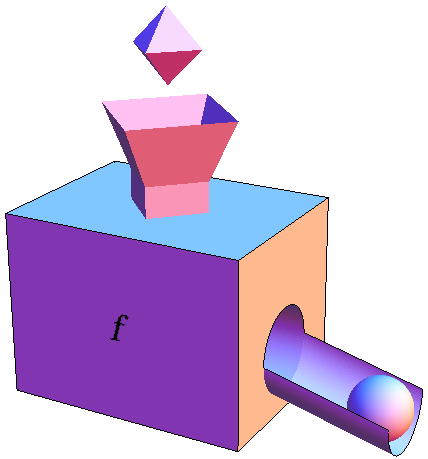
\includegraphics[width=\textwidth]{../Mathematik_1/Bilder/funktionen_maschinenmodell.png}
\end{minipage}
\begin{minipage}{0.56\textwidth}
	Die Maschine \(f\) produziert zu jedem \(x\in D\) ein \(y\in Z\). Den "\,Produktionsprozess"\, umkehren bedeutet eine Maschine \(f^{-1}\) zu finden, die jedem von \(f\) produzierten \(y\) sein Urbild, also seinen zugeh�rigen \(x\)-Wert, zuordnet, also so: 
\end{minipage}
\begin{minipage}{0.2\textwidth}
		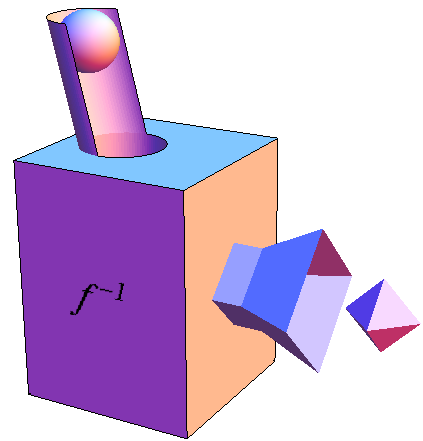
\includegraphics[width=\textwidth]{../Mathematik_1/Bilder/funktionen_umkehrfunktion_maschinenmodell.png}
\end{minipage}
\end{exabox}

Ist die Funktion als Graph gegeben, l��t sich die Frage nach der Existenz einer Umkehrfunktion leicht beantworten. Drehen wir den Graph so, dass die \(y\)-Achse waagerecht und die \(x\)-Achse senkrecht erscheint, und �berpr�fen, ob die gedrehte Figur eine Funktion ist:
\begin{itemize}
	\item[\(\Rightarrow\)] Falls ja, dann kann man \(f\) auf \(D\) umkehren!
	\item[\(\Rightarrow\)] Falls nein, dann gibt es keine Umkehrfunktion, zumindest nicht auf \(D\)! 
\end{itemize}
Was sagen Sie zum n�chsten Beispiel: besitzt die Funktion \(f: x\mapsto x^2\) eine Umkehrfunktion?\footnote{Die Normalparabel ist nicht umkehrbar, weil es kein eindeutiges "\,Zur�ck\"\, gibt.}
\begin{exabox}{Graphische L�sung: dreh den Graph um!}{ } 
	\begin{center}
		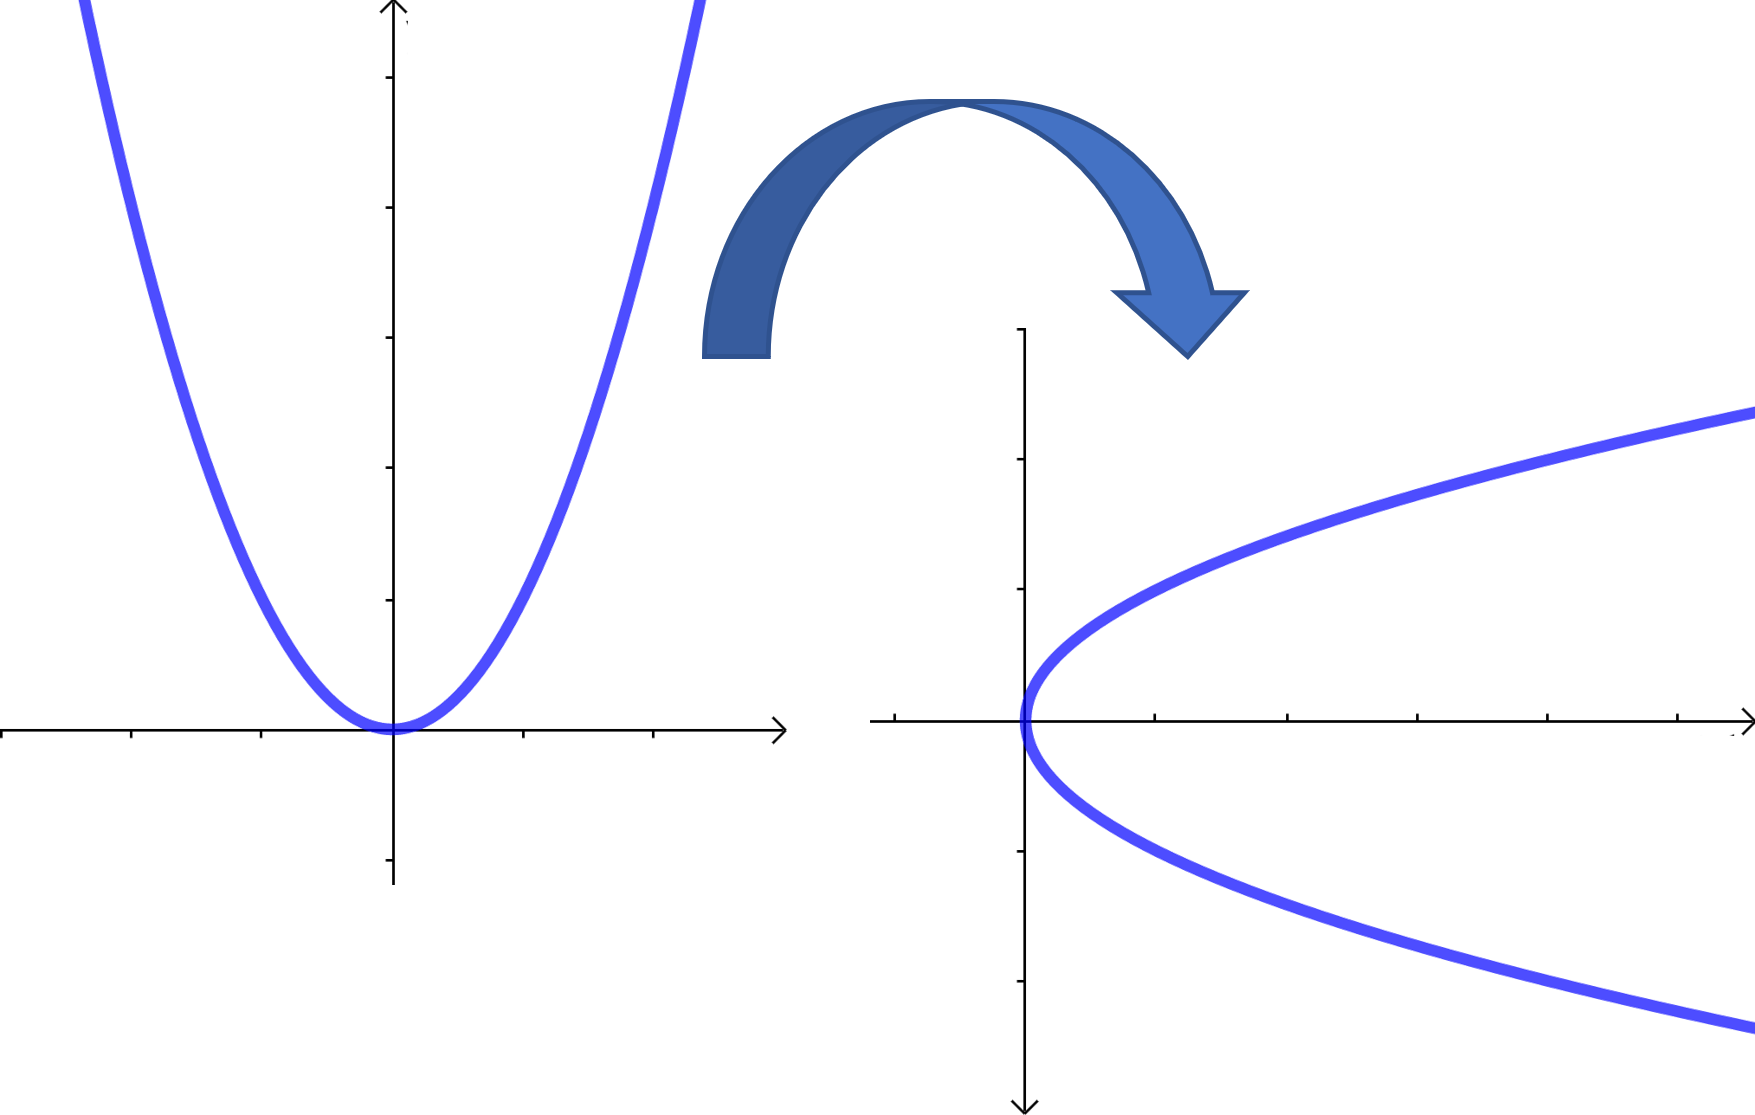
\includegraphics[width=0.6\textwidth]{../Mathematik_1/Bilder/funktionen_umkehrbarkeit_normalparabel_gedreht.png}
\end{center}
\end{exabox}

Die mathematischen Bedingungen daf�r, dass die gedrehte Figur der Graph einer Funktion ist, lauten :
  \begin{itemize}
	  \item Ein Funktionswert \(y\) im Zielmenge \(Z\) von \(f\) wird genau einmal erreicht. (Injektivit�t von \(f\) )
	  \item Jeder Funktionswert \(y\) im Bildmenge \(Z\) von \(f\) erreicht. (Surjektivit�t von \(f\) )
  \end{itemize}
  Gelten diese beiden Bedingungen, dann nennt man \(f\) bijektiv. F�r bijektive Funktionen l��t sich eine Umkehrfunktion bestimmen. In mathematischer Kurzschreibweise l��t sich die Bijektivit�t von \(f\) wie folgt definieren: 
\begin{defbox}{Existenz einer Umkehrfunktion}{ }
	\(f\) ist genau dann umkehrbar, wenn \(f\) bijektiv ist, wenn also gilt
  \begin{itemize}
	  \item $x,y\in D:\; f(x) = f(y)\, \Leftrightarrow\, x=y\,.$ (Injektivit�t)
	  \item $\forall\, y \in Z \, \exists\, x\in D:\; f(x) = y\;$ oder kurz \; $f(D) = Z$. (Surjektivit�t)
  \end{itemize}
\end{defbox}

\begin{exabox}{Injektivit�t? links ja, rechts nein!}{ } %Bild streng monotone Funktion ist umkehrbar
	\centering
	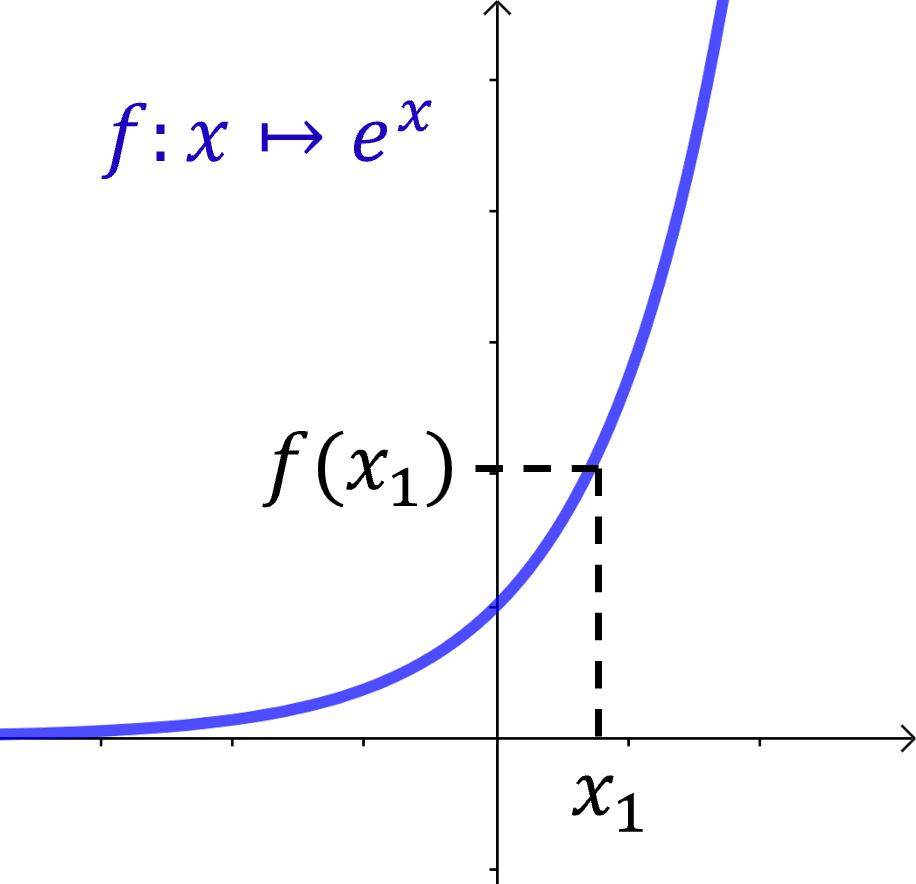
\includegraphics[width=0.25\textwidth]{../Mathematik_1/Bilder/funktionen_injektivitaet_exponentialfunktion.png}\hspace{3cm}
	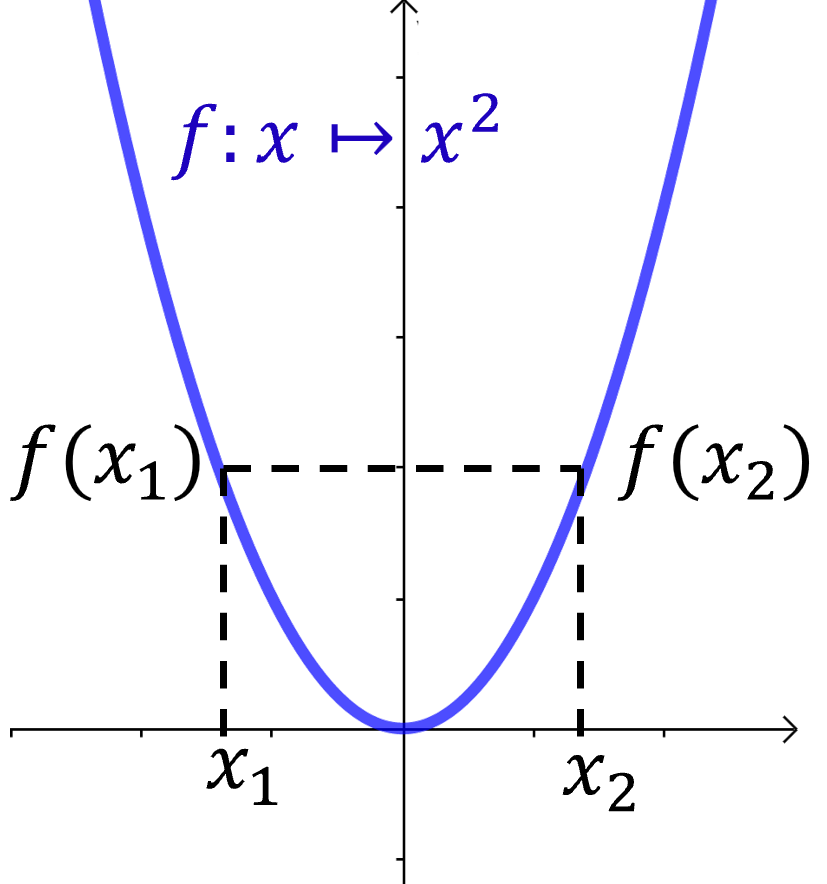
\includegraphics[width=0.25\textwidth]{../Mathematik_1/Bilder/funktionen_injektivitaet_quadratfunktion_gegenbeispiel.png}
\end{exabox}

%Die Funktionswerte \(y\) einer Funktion \(f: x\mapsto f(x) \)   Stellen Sie sich vor, dass Sie eine Funktionsabbildung gegeben haben, beispielsweise   finden Sie praktisch heraus, in dem Sie einen Funktionsgraphen um \(90\circ\) drehen und analysieren, ob die Figur, die Sie sehen eine Funktion ist oder nicht. Wir werden uns mit der
%Um  eine  Gleichung  wie $a+3=5$ nach $a$ aufzul�sen,  wendet  man  (strenggenommen) auf beide Seiten eine Funktion, n�mlich $x\mapsto x-3$, an:
%
%\begin{exabox}{Umkehrfunktion $\Rightarrow$ Aufl�sen einer Gleichung}{ }
%  $ a+ 3 = 5 \Leftrightarrow a+3-3 = 5-3 \Leftrightarrow a = 2\,.$
%\end{exabox}
%
%Um $e^b=7$ nach $b$ aufzul�sen wendet man entsprechend den nat�rlichen Logarithmus $x\mapsto \ln(x)$ an (warum ist das hier kein Problem?)
%
%\begin{exabox}{Umkehrfunktion $\Rightarrow$ Aufl�sen einer Gleichung}{ }
%  $e^b = 7 \Leftrightarrow \ln(\mathrm{exp}(b)) = \ln(7) \Leftrightarrow b = \ln(7)\,.$
%\end{exabox}

%Man sucht also Funktionen, welche die urspr�nglichen Funktionen wieder aufheben, sie umkehren:
%\begin{center}
%  \begin{tabular}{l|l}
%    Funktion & Idee Umkehrfunktion \\
%    \hline
%    $x\mapsto x+3$ & $x+3 \mapsto x$ \\
%    $x\mapsto \mathrm{exp}(x) $ &  $\mathrm{exp}(x) \mapsto x$ 
%  \end{tabular}
%\end{center}

Soweit zur Theorie, die spannendere Frage ist: wie bestimmen wir die Abbildungsvorschrift der \textbf{Umkehrfunktion} (\emph{inverse function})? 

\noindent{\textbf{Bemerkungen}}
\begin{itemize}
	\item Ist \(f\) eine \textbf{diskrete}, \textbf{bijektive} Funktion, gegeben als zweispaltige Tabelle, dann erh�lt man die Umkehrfunktion durch Vertauschen der beiden Spalten!\marginpar{Aufgabe} Die Tabelle l��t sich n�mlich einfach r�ckw�rts lesen und man erh�lt wieder eine Funktion: die Umkehrfunktion  $f^{-1}:Z\to D$. Der Definitionsbereich und die Zielmenge sind gegen�ber der Originalfunktion $f:D\to Z$ vertauscht. 
	\item Ist \(f\) eine \textbf{bijektive} Funktion, deren Funktionsabbildung gegeben ist, dann erh�lt man die Umkehrfunktion \(f^{-1}\), indem man die Abbildungsvorschrift \( y = f(x) \) nach \(x\) aufl�st. 
\end{itemize}


\begin{exabox}{Bestimmung der Umkehrfunktion}{ }
	\begin{itemize}
		\item $f:\mathbb R\to \mathbb R, \; x\mapsto \displaystyle{\frac12} \cdot x + 1 $ ist bijektiv, also 
			\begin{eqnarray*} 
					\begin{array}{lrlll}
						& y &=& \displaystyle{\frac12} \cdot x+1 &\; \| -1 \\[2ex]
						\Leftrightarrow & y-1 &=& \displaystyle{\frac12}\cdot x &\; \| \cdot 2 \\[2ex]
				\Leftrightarrow & 2\cdot y-2 &=& x &\;\Rightarrow  \; f^{-1}: \mathbb R\to \mathbb R, \; x\mapsto 2\cdot x-2\end{array}\end{eqnarray*}
			\item $f: (3,\infty)\to (0,\infty), \; x\mapsto \displaystyle{ \frac{2}{x-3}}$ ist bijektiv, also 
			\begin{eqnarray*} 
					\begin{array}{lrlll}
						&y &=&  \displaystyle{ \frac{2}{x-3}} & \|\cdot (x-3) \quad (x\not=3!) \\[2ex]
						\stackrel{x\not=3}{\Leftrightarrow} & (x-3) \cdot y &=& 2 & \| : y \quad (\not=0!) \\[2ex]
						\stackrel{y\not=0}{\Leftrightarrow} & x-3 &=& \displaystyle{\frac{2}{y} } &\|+3 \\[2ex]
						\Leftrightarrow & x &=& \displaystyle{\frac{2}{y} }+3 &  \;\Rightarrow \;  f^{-1}: (0,\infty) \to (3,\infty), \; x\mapsto \displaystyle{ \frac2x } +3
				\end{array}
			\end{eqnarray*}
	\end{itemize}
\end{exabox}

%\begin{exabox}{Bestimmung der Umkehrfunktionen}{ }
%	\begin{eqnarray*} 
%		f_1: x\mapsto x+3 & \Rightarrow & y = x+3 \Leftrightarrow x = y-3 \Rightarrow f_1^{-1}: x\mapsto x-3 \\ 
%		f_2: x\mapsto e^x & \Rightarrow & y = e^x \Leftrightarrow x = \ln(y) \Rightarrow f_2^{-1}: x \mapsto \ln(x) \,. 
%	\end{eqnarray*}
%\end{exabox}

\begin{theorembox}{Systematische Bestimmung der Umkehrfunktion}{ }
	\begin{enumerate}
		\item Bestimmung des Bildbereichs $W_f =f(D)\subset Z$ von $f$ (Surjektivit�t). 
		\item Bestimmung der Teilmenge $X\subseteq D$, auf der $f$ injektiv ist (Injektivit�t).
		\item L�sen der Gleichung $y=f(x)$ f�hrt auf $x=g(y)$. 
		\item Definition der Umkehrfunktion $ f^{-1}: W_f \to X, \; x\mapsto g(x)\,.$
	\end{enumerate}
\end{theorembox}

	\noindent\textbf{Bemerkungen:}
\begin{itemize} 
	\item Der Index $-1$ ist eine mathematische Notation -- sie hat nichts mit dem Kehrwert zu tun\footnote{Sp�ter bezeichnet $f^{42}$, dass die Funktion $f$ $42$-mal hintereinander anzuwenden ist, also $f^{42}(x)=f(f(\cdots 42-\mathrm{mal} \cdots f(x)\cdots))$. Die Notation mit $-1$ setzt diesen Gedanken fort und $f^0$ wird eingef�hrt als (komplizierte) Bezeichnung f�r die identische Abbildung: $f^0: x\mapsto x\,.$}.
	\item Wenn man zuerst die Funktion $f$ und dann auf das Resultat davon die dazugeh�rige Umkehrfunktion $f^{-1}$ anwendet (oder andersherum), dann erh�lt man die identische Abbildung \(\mathrm{id}: x\mapsto x\):
		\begin{theorembox}{$ \mathrm{id} = f \circ f^{-1} = f^{-1} \circ f$}{ }
  \begin{itemize}
	  \item[$\bullet$] $x \mapsto f^{-1}\big( f(x)\big) = x\,,$
	  \item[$\bullet$] $x \mapsto f\left( f^{-1}(x)\right) = x\,.$
\end{itemize}
\end{theorembox}
	\item In der praktischen  Ingenieurmathematik  k�mmert  man  sich  wenig  um  die Surjektivit�t. Denn ist eine Funktion injektiv, aber nicht surjektiv, kann man diesen Mangel leicht durch Anpassung der Zielmenge heilen. Zum Beispiel ist $f: \mathbb R \to \mathbb R, \, x\mapsto e^x$ nicht surjektiv, aber $f: \mathbb R \to (0,\infty), \, x\mapsto e^x$ ist surjektiv. 
\end{itemize}


Unter den folgenden Funktionen sind zwei, die umkehrbar sind. Wissen Sie welche?
\begin{itemize}
  \item $f_1: \mathbb R \to \mathbb R $ mit $x\mapsto \textnormal{kaufm\"annische Rundung von } x \textnormal{ auf eine Stelle nach dem Komma}$ 
  \item $f_2: \mathbb R \to \mathbb R$ mit $ x\mapsto x^2$
  \item $f_3: [0,8) \to \mathbb R$ mit $x\mapsto x^2$
  \item $f_4: [0,4) \to [0,16)$ mit $x\mapsto x^2$
  \item $f_5: \mathbb R \to \mathbb R$ mit $x\mapsto \sin(x)$
  \item $f_6: [-\pi/2,\pi/2] \to \mathbb R $ mit $x\mapsto \sin(x)$
  \item $f_7: [-\pi/2,\pi/2] \to [-1, 1] $ mit $ x \mapsto \sin(x)$
\end{itemize}
  % Eigenschaften von Funktionen
\newpage
\setcounter{satz}{0} \setcounter{def}{0} \setcounter{exa}{0}  \section{Lineare Funktionen}\label{MA1-lineare-funktionen}

\begin{table}[H]
  \centering
  \begin{tabularx}{\textwidth}{p{0.9\textwidth} p{0.1\textwidth}}
    \toprule
	  \multicolumn{2}{c}{\textbf{�bersicht �ber Lernziele und Voraussetzungen}}\\
    \midrule
    \textbf{Lernziele} &\\[.5\normalbaselineskip]
    \tabitem lineare Funktionen in verschiedenen Darstellungsformen angeben und ineinander �berf�hren: &\\
    \hspace{0.7cm}\tabitem Achsenabschnittsform &\\
    \hspace{0.7cm}\tabitem Zwei-Punkte-Form &\\
    \hspace{0.7cm}\tabitem Punkt-Steigungs-Form &\\
    \tabitem st�ckweise definierte Funktionen lesen und interpretieren &\\
    \tabitem eine gegebene Messreihe durch lineare Interpolation mit einem linearen Spline beschreiben &\\
    \tabitem Interpolation und lineare Regression voneinander unterscheiden &\\
    \tabitem f�r eine Messreihe eine Ausgleichsgerade mittels linearer Regression bestimmen &\\
    \midrule
	  \textbf{Voraussetzungen} \\[.5\normalbaselineskip]
	  \tabitem Grundrechenarten & \abschnittsverweis{MA1-zahlenmengen}\\
	  \tabitem �quivalenzumformungen & \abschnittsverweis{MA1-aequivalenzumformungen}\\
	  \tabitem Definition einer Funktion & \abschnittsverweis{MA1-funktionen}\\
    \bottomrule
  \end{tabularx}
\end{table}

\ifintegriereaufgaben \noindent �bungsaufgaben zum Thema finden Sie hier: \hyperref[MA1-lineare-funktionen-aufgaben]{Aufgaben}
\vspace{0.3cm}
\hrule
\fi

\subsection{Lineare Funktionen}

Funktionen der Art $f: \mathbb R \to \mathbb R$ mit $x\mapsto 2\cdot x+3$ hei�en \textbf{linear}\footnote{In der Schulmathematik und elementaren Analysis werden Funktionen der Form \(f(x)=mx+b\) �blicherweise als lineare Funktionen bezeichnet. Im Sinne der linearen Algebra handelt es sich f�r \(b\neq0\) um affine Abbildungen; eine lineare Abbildung muss insbesondere \(f(0)=0\) erf�llen.}

Der Graph einer linearen Funktion ist eine Gerade, aber keine vertikale Gerade\footnote{Eine vertikale Gerade kann nicht Graph einer Funktion \(x\mapsto f(x)\) sein, da zu derselben \(x\)-Koordinate mehrere \(y\)-Werte geh�ren w�rden.}
In der Form

$$
f(x)=m \cdot x+b
$$

beschreibt \(m\) die \textbf{Steigung} der Geraden und \(b=f(0)\) ihren Schnittpunkt mit der \(y\)-Achse. Je nachdem, welche Informationen �ber eine Gerade gegeben sind, sind jedoch unterschiedliche Darstellungsformen zweckm��ig.

\begin{itemize}
	\item Angenommen \(f\) schneidet die $x$-Achse an der Stelle $a\in D$ mit \(a\not=0\) und \(f\) schneidet die $y$-Achse im Punkt $(0,b)\in D\times Z$ mit \(b\not=0\), dann kann man die Abbildungsvorschrift der lineare Funktion in \textbf{Achsenabschnittsform} angeben:
		\[ 
			f(x) = \displaystyle{-\frac{b}{a}}\cdot x + b.
  \]
Dass diese Gleichung tats�chlich richtig ist, kann man so sehen: sie beschreibt eine Gerade und stimmt f�r die beiden Schnittpunkte mit den Achsen. Eine  andere  Gerade  als  die  gesuchte  w�rde  aber  nicht  durch  diese  beiden Schnittpunkte verlaufen. 

\item F�r zwei voneinander verschiedene Punkte  $(x_1|y_1)$ und $(x_2|y_2)$, die auf einer nichtvertikalen Geraden liegen, ist das Verh�ltnis von \(y_2 - y_1\) zu \(x_2 - x_1\) immer gleich! Der Wert wird \textbf{Steigung der Gerade} genannt:
	\[ 
  m = \displaystyle{\frac{y_2-y_1}{x_2-x_1}}.
  \]
Kennt man die Steigung \(m\) der Gerade und einen Punkt \( (x_1|y_1)\) auf der Gerade, dann ist die Gerade eindeutig bestimmt. Die \textbf{Punkt-Steigungs-Form} liefert die Abbildungsvorschrift: 
\[ 
	f(x) = m\cdot (x-x_1) + y_1.
\]
\item Kennt man anstatt der Steigung einen weiteren Punkt, gibt man die Gerade in \textbf{Zwei-Punkte-Form} an:

	\[ f(x) = \displaystyle{\frac{y_2-y_1}{x_2-x_1}}\cdot (x-x_1) + y_1.\]
	\end{itemize}


\begin{exabox}{Lineare Funktion \(f: x\mapsto 2\cdot x+3\)}{ }
\begin{minipage}{0.3\textwidth}
	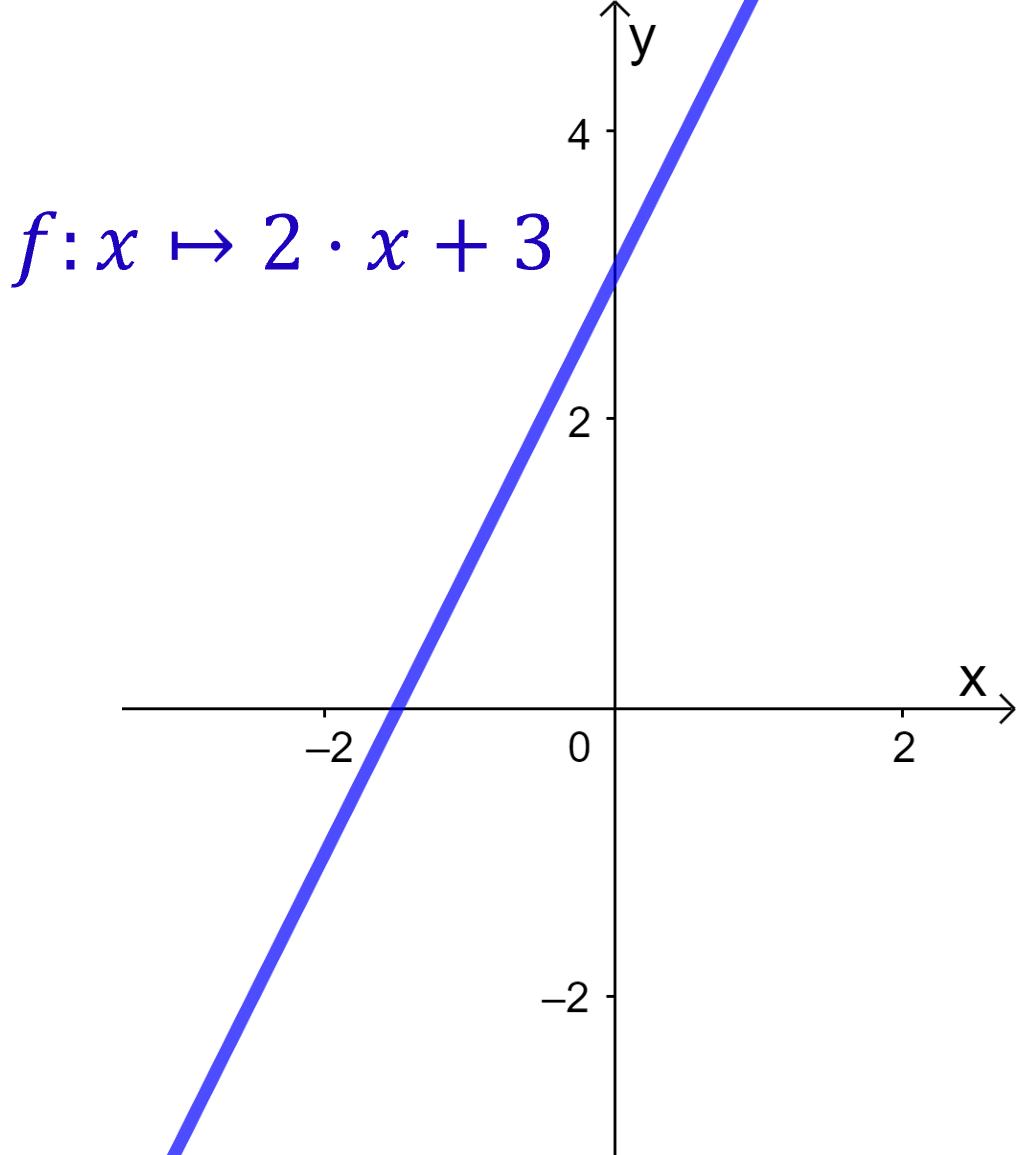
\includegraphics[width=\textwidth]{../Mathematik_1/Bilder/lineare_funktionen_gerade_zwei_x_plus_drei.png}
	\end{minipage}
	\begin{minipage}{0.7\textwidth}
		Unterschiedliche Darstellungen f�r \(f\):
		\begin{itemize}
			\item Achsenabschnitt-Form:
				\[a=-\frac32, \; b = 3: \quad f(x) = - \dfrac{3}{-\frac32}\cdot x + 3 = 2\cdot x+3 \]
			\item Punkt-Steigungs-Form:
				\[m=2, \; P(1|5):\quad f(x) = 2\cdot \left( x- 1\right) + 5 = 2\cdot x+3 \]
			\item Zwei-Punkte-Form:
				\[P_1(0|3),\; P_2(1|5): \quad f(x) =  \dfrac{3-5}{0-1}\cdot \left( x- 1\right) + 5  = 2\cdot x+3\,.\]
		\end{itemize}
	\end{minipage}
\end{exabox}

\subsection{Interpolation mit Linearen Funktionen}

In einer der folgenden Anwendungen wird der Begriff "\,st�ckweise definierte Funktion"\, benutzt:

\begin{defbox}{St�ckweise definierte Funktion}{ }
Eine Funktion hei�t \textbf{st�ckweise definiert} (\emph{piecewise defined}), wenn f�r verschiedene Teilbereiche ihres Definitionsbereichs unterschiedliche Abbildungsvorschriften gelten.

Beispielsweise kann eine Funktion die Form

$$
f(x)=
\begin{cases}
f_1(x), & x\in D_1,\\
f_2(x), & x\in D_2,\\
\vdots\\
f_n(x), & x\in D_n
\end{cases}
$$

besitzen, wobei

$$
D=D_1\cup D_2\cup \cdots \cup D_n.
$$

Dabei muss f�r jedes \(x\in D\) eindeutig festgelegt sein, welche Abbildungsvorschrift gilt.
	
	%Von einer st�ckweise definierten Funktion \(f: D\to \mathbb R\) ist dann die Rede, wenn man den Definitionsbereich in \(N-1\) Intervalle \[I_k= [x_k, x_{k+1}], \; x_k < x_{k+1}, \; k=1,\cdots, N-1, \] aufteilen kann, also \[ D = \bigcup\limits_{k=1}^{N-1} I_k = [x_1, x_N]\,,\] und wenn sich auf jedem der Intervalle \(I_k\) eine geschlossene Abbildungsformel angeben l��t: \[ f:x\mapsto \begin{cases} f_1(x), \quad x\in I_1,\\[2ex] f_2(x),\quad x\in I_2, \\[1ex] \vdots \\ f_{N-1}(x), \quad x\in I_{N-1}\,.\end{cases}\] 
\end{defbox}
	%Die Frage, ob eine st�ckweise definierte Funktion auf ihrem Definitionsbereich stetig oder sogar differenzierbar ist, h�ngt offensichtlich damit zusammen, wie glatt die Funktion von einem Intervall zum anderen Intervall �bergeht. 
Der Prototyp einer st�ckweise definierten Funktion ist die Betragsfunktion:\marginpar{Aufgabe} 
	\begin{exabox}{Betragsfunktion}{ }
		$ f:x\mapsto |x| = \begin{cases} x, &\quad x \in [0, \infty)\,, \\ -x, &\quad x\in (-\infty,0)\,.\end{cases} $
\end{exabox}

Liegt eine Messreihe vor, so wurde eine Gr��e \(y\) f�r verschiedene Werte einer anderen Gr��e \(x\) bestimmt. Ein Beispiel ist die elektrische Leitf�higkeit eines Metallblocks in Abh�ngigkeit von seiner Temperatur.

Die Messdaten bestehen aus \(N\) Messpunkten

$$
\{(x_i,y_i):i=1,\dots,N\}.
$$

Dabei seien die Messstellen aufsteigend geordnet $ x_1<x_2<\dots<x_N$.

Soll eine Funktion konstruiert werden, deren Graph durch s�mtliche Messpunkte verl�uft, spricht man von einer \textbf{Interpolation} (\emph{interpolation}). Eine besonders einfache M�glichkeit besteht darin, jeweils zwei benachbarte Messpunkte durch eine Gerade zu verbinden. Auf jedem Intervall

$$
I_k=[x_k,x_{k+1}]
$$

wird also die Zwei-Punkte-Form einer Geraden verwendet. Auf diese Weise entsteht ein \textbf{linearer Spline} (\emph{linear spline}).

%Nehmen wir uns liegt eine Messreihe vor: eine physikalische Gr��e \(y\) wurde in Abh�ngigkeit einer anderen Gr��e \(x\) gemessen\footnote{Zum Beispiel die Leitf�higkeit eines Metallblocks in Abh�ngigkeit von seiner Temperatur.}. Die Messdaten bestehen dann also aus einer Menge von \(N\) Messpunkten \[ \left\{ \left( x_i| y_i\right), \; x_i, y_i \in \mathbb R,\; i=1,\dots,N\right\} \] und zur Analyse der Daten suchen wir eine Funktion, deren Graph die Messpunkte durchl�uft.\marginpar{Aufgabe} Wir suchen eine Funktion, die die Daten \textbf{interpoliert}. Eine Idee ist die folgende: zwischen zwei aufeinanderfolgenden Messwerten wird linear interpoliert --  auf diese Weise wird ein \textbf{linearer Spline} konstruiert. Die Details fasst die folgende Regel zusammen.  

\begin{defbox}{Linearer Spline}{ }
	Es seien \(N\) Messpunkte \( \{(x_i| y_i),\; x_i, y_i \in \mathbb R\,, \; i=1,\cdots,N, \text{ und } x_1<x_2< \cdots <x_N \} \) gegeben. Mit 
$$
I_k=[x_k,x_{k+1}], \; k=1,\ldots,N-1, 
$$
lautet der lineare Spline
	
	\begin{eqnarray*}
		f: [x_1,x_N] \to\mathbb R,\; x\mapsto \begin{cases} \displaystyle{\frac{y_2-y_1}{x_2-x_1}}\cdot (x-x_1) + y_1, \quad x\in I_1\,,\\[2ex]  \displaystyle{\frac{y_3-y_2}{x_3-x_2}}\cdot (x-x_2) + y_2, \quad x\in I_2\,,\\  \vdots \\  \displaystyle{\frac{y_N-y_{N-1}}{x_N-x_{N-1}}}\cdot (x-x_{N-1}) + y_{N-1}, \quad x\in I_{N-1}\,.\end{cases}
	\end{eqnarray*}
\end{defbox}

Ein linearer Spline ist nichts anderes als die wiederholte Anwendung der Zwei-Punkte-Form auf benachbarte Messpunkte.

\subsection{Lineare Regression }

Bei einer Interpolation wird verlangt, dass der Graph der konstruierten Funktion s�mtliche Messpunkte exakt durchl�uft. F�r Messdaten ist diese Forderung jedoch nicht immer sinnvoll. Messwerte sind h�ufig mit Messfehlern und anderen Unsicherheiten behaftet, sodass kleine Abweichungen einzelner Punkte nicht unbedingt Teil des zugrunde liegenden funktionalen Zusammenhangs sind.

In einer solchen Situation wird statt einer exakt interpolierenden Funktion eine Funktion gesucht, welche die Gesamtheit der Messdaten m�glichst gut beschreibt. Soll dieser Zusammenhang durch eine Gerade modelliert werden, f�hrt dies zur \textbf{linearen Regression} (\emph{linear regression}).

Gesucht ist eine lineare Funktion \(f:x\mapsto mx+b\), f�r welche die Summe der quadrierten vertikalen Abweichungen von den Messwerten minimal wird. 

Die \textbf{Abweichung} oder das \textbf{Residuum} (\emph{residual}) des \(i\)-ten Messwerts von der Geraden betr�gt

$$ r_i=f(x_i) - y_i = m\cdot x_i+b-y_i. $$

Bei der Bestimmung der linearen Regression werden \(m\) und \(b\) so gew�hlt, dass die Summe aller quadrierten Abweichungen

$$ r_1^2+\dots+r_N^2 $$

m�glichst klein wird: 

\[ \sum\limits_{i=1}^N \left( m \cdot x_i + b - y_i \right)^2 \stackrel{!}{=} \min \,.\]
F�r verschiedene Messstellen \(x_i\) ist die Aufgabe eindeutig l�sbar mit expliziten Formeln f�r die optimalen Werte von $m$ und $b$:\marginpar{Aufgabe} 

\begin{theorembox}{Ausgleichsgerade (lineare Regression oder Bestapproximation)}{ }
	Die Ausgleichsgerade \[ f: x\mapsto m\cdot x + b \] f�r $N$ verschiedene Messpunkte $\{ (x_1, y_1), (x_2,y_2), \dots, (x_N, y_N)\}$ mit $x_1 < x_2 < \cdots < x_n$ besitzt die Steigung  
	\begin{eqnarray*} 
		m = \frac{\sum\limits_{i=1}^N (x_i - \langle x\rangle ) \cdot (y_i - \langle y\rangle ) }{ \sum\limits_{i=1}^N (x_i - \langle x \rangle )^2 }
		\end{eqnarray*}
		und den \(y\)-Achsenabschnitt 
		\begin{eqnarray*}
		b = \langle y \rangle - m \cdot \langle x\rangle\,.
	\end{eqnarray*} 
	Die spitzen Klammern $\langle \cdot  \rangle $ bezeichnen Mittelwerte, also
	\begin{eqnarray*}
		\langle x \rangle = \frac{1}{N} \cdot \sum\limits_{i=1}^N x_i\,, \quad \langle y \rangle = \frac{1}{N}\cdot \sum\limits_{i=1}^N y_i\,.
	\end{eqnarray*}
\end{theorembox}

\noindent{\textbf{Bemerkung:}}
\begin{itemize}
	\item Die Ausgleichsgerade verl�uft damit durch den Punkt $ \big(\langle x\rangle,\langle y\rangle\big), $ also durch den Schwerpunkt der Messpunkte.
	\item Die Ausgleichsgerade interpoliert alle Messpunkte, wenn die Messpunkte exakt auf einer Geraden liegen.
	\item Die Ausgleichsgerade reagiert sensitiv auf \textbf{Ausrei�er} in der Messreihe, weil die Abst�nde quadriert werden. 
\end{itemize}

\begin{exabox}{Lineare Regression}{}

Gegeben seien die drei Messwerte

$$
(1,2),\qquad (2,3),\qquad (3,5).
$$

Gesucht ist daher eine Ausgleichsgerade, die die drei Messwerte im Sinne der kleinsten Quadrate m�glichst gut beschreibt.

\begin{itemize} 
	\item Zun�chst werden die Mittelwerte der \(x\)- und \(y\)-Werte bestimmt:

$$
\langle x\rangle = \frac{1+2+3}{3} = 2, \quad \langle y\rangle = \frac{2+3+5}{3} = \frac{10}{3}.
$$

\item Die Steigung der Ausgleichsgerade l�sst sich nun berechnen:

$$
\begin{aligned}
m
&=
\frac{
\displaystyle
\sum_{i=1}^3
(x_i-\langle x\rangle)
(y_i-\langle y\rangle)
}{
\displaystyle
\sum_{i=1}^3
(x_i-\langle x\rangle)^2
}
\\[1ex]
&=
\frac{
(1-2)\left(2-\frac{10}{3}\right)
+
(2-2)\left(3-\frac{10}{3}\right)
+
(3-2)\left(5-\frac{10}{3}\right)
}{
(1-2)^2+(2-2)^2+(3-2)^2
}
\\[1ex]
&=
\frac{
\frac43+0+\frac53
}{
1+0+1
}
=
\frac{3}{2}.
\end{aligned}
$$

\item Damit ergibt sich f�r den \(y\)-Achsenabschnitt 

$$
b
=
\frac{10}{3}
-
\frac32\cdot2
=
\frac13.
$$
\end{itemize}

Die gesuchte Ausgleichsgerade lautet damit $f(x)=\frac32x+\frac13$.

	\begin{minipage}{0.5\textwidth}
		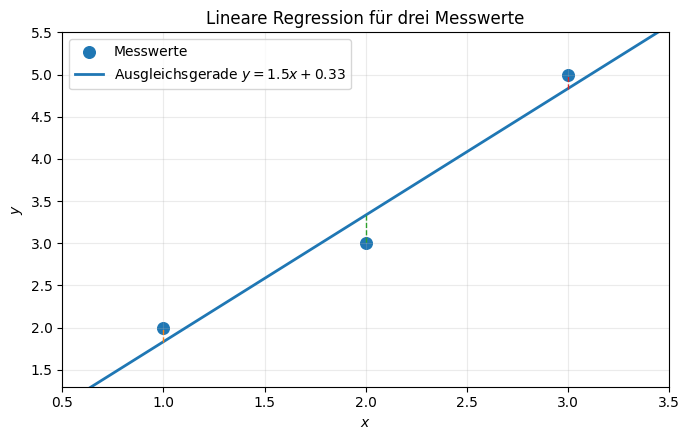
\includegraphics[width=\textwidth]{../Mathematik_1/Bilder/lineare_regression_drei_messwerte.png}
\end{minipage}
\begin{minipage}{0.5\textwidth}
	\begin{itemize}
		\item Im Unterschied zu einer Interpolation verl�uft die Ausgleichsgerade im Allgemeinen nicht durch die Messpunkte. 
		\item Die gestrichelten vertikalen Linien in der Abbildung zeigen die Abweichungen zwischen den Messwerten und den zugeh�rigen Werten der Ausgleichsgeraden.
	\end{itemize}
\end{minipage}

\end{exabox}
  % Lineare Funktionen
\newpage
\setcounter{satz}{0} \setcounter{def}{0} \setcounter{exa}{0}  

\section{Potenzfunktionen und Wurzelfunktionen}\label{MA1-potenz-und-wurzelfunktionen}

\begin{table}[H]
  \centering
  \begin{tabularx}{\textwidth}{p{0.9\textwidth} p{0.1\textwidth}}
    \toprule
	  \multicolumn{2}{c}{\textbf{�bersicht �ber Lernziele und Voraussetzungen}}\\
    \midrule
	  \textbf{Lernziele} &\\[.5\normalbaselineskip]
	  \tabitem Potenzfunktionen und Wurzelfunktionen skizzieren &\\
	  \tabitem Monotonie und Symmetrie einer Potenzfunktion charakterisieren &\\
\tabitem Wurzelfunktionen als Umkehrfunktionen geeigneter Potenzfunktionen vestehen &\\
\tabitem Definitionsbereiche von Wurzelfunktionen bestimmen &\\
\tabitem Gleichungen mit Potenzen und Wurzeln unter Beachtung des Definitionsbereichs l�sen &\\
\tabitem Potenzrechenregeln mit ganzzahligem und gebrochenzahligem Exponenten anwenden &\\
    \midrule
	  \textbf{Voraussetzungen} \\[.5\normalbaselineskip]
	  \tabitem Grundrechenarten & \abschnittsverweis{MA1-zahlenmengen}\\
	  \tabitem �quivalenzumformungen & \abschnittsverweis{MA1-aequivalenzumformungen}\\
	  \tabitem Injektivit�t, Bijektivit�t, Umkehrbarkeit  & \abschnittsverweis{MA1-funktionen}\\
    \bottomrule
  \end{tabularx}
\end{table}

 \ifintegriereaufgaben \noindent �bungsaufgaben zum Thema sind hier: \hyperref[MA1-potenz-und-wurzelfunktionen-aufgaben]{Aufgaben}
\vspace{0.3cm}
\hrule
 \fi

\subsection{Potenzfunktionen} 


Eine Funktion der Form
\[
f:\mathbb R\to\mathbb R,\qquad x\mapsto x^n,
\]
mit \(n\in\mathbb N^+\) hei�t Potenzfunktion (\emph{power function}). Der Definition \underline{Definitionsbereich}\randverweis{MA1-funktionen} aller dieser Potenzfunktionen \footnote{Auch Funktionen wie \(x\mapsto x^{-1/5}\) oder \(x\mapsto x^\pi\) geh�ren zu allgemeineren Potenzfunktionen.  Ihre Definitionsbereiche erfordern jedoch zus�tzliche �berlegungen: \(x^{-1/5}\) ist bei \(x=0\) nicht definiert, w�hrend \(x^\pi\) im Reellen f�r negative \(x\) nicht definiert ist.} ist \(\mathbb R\).

\begin{theorembox}{Monotonie und Symmetrie von Potenzfunktionen mit geradem Exponenten}{ }
	\begin{minipage}{0.35\textwidth}
	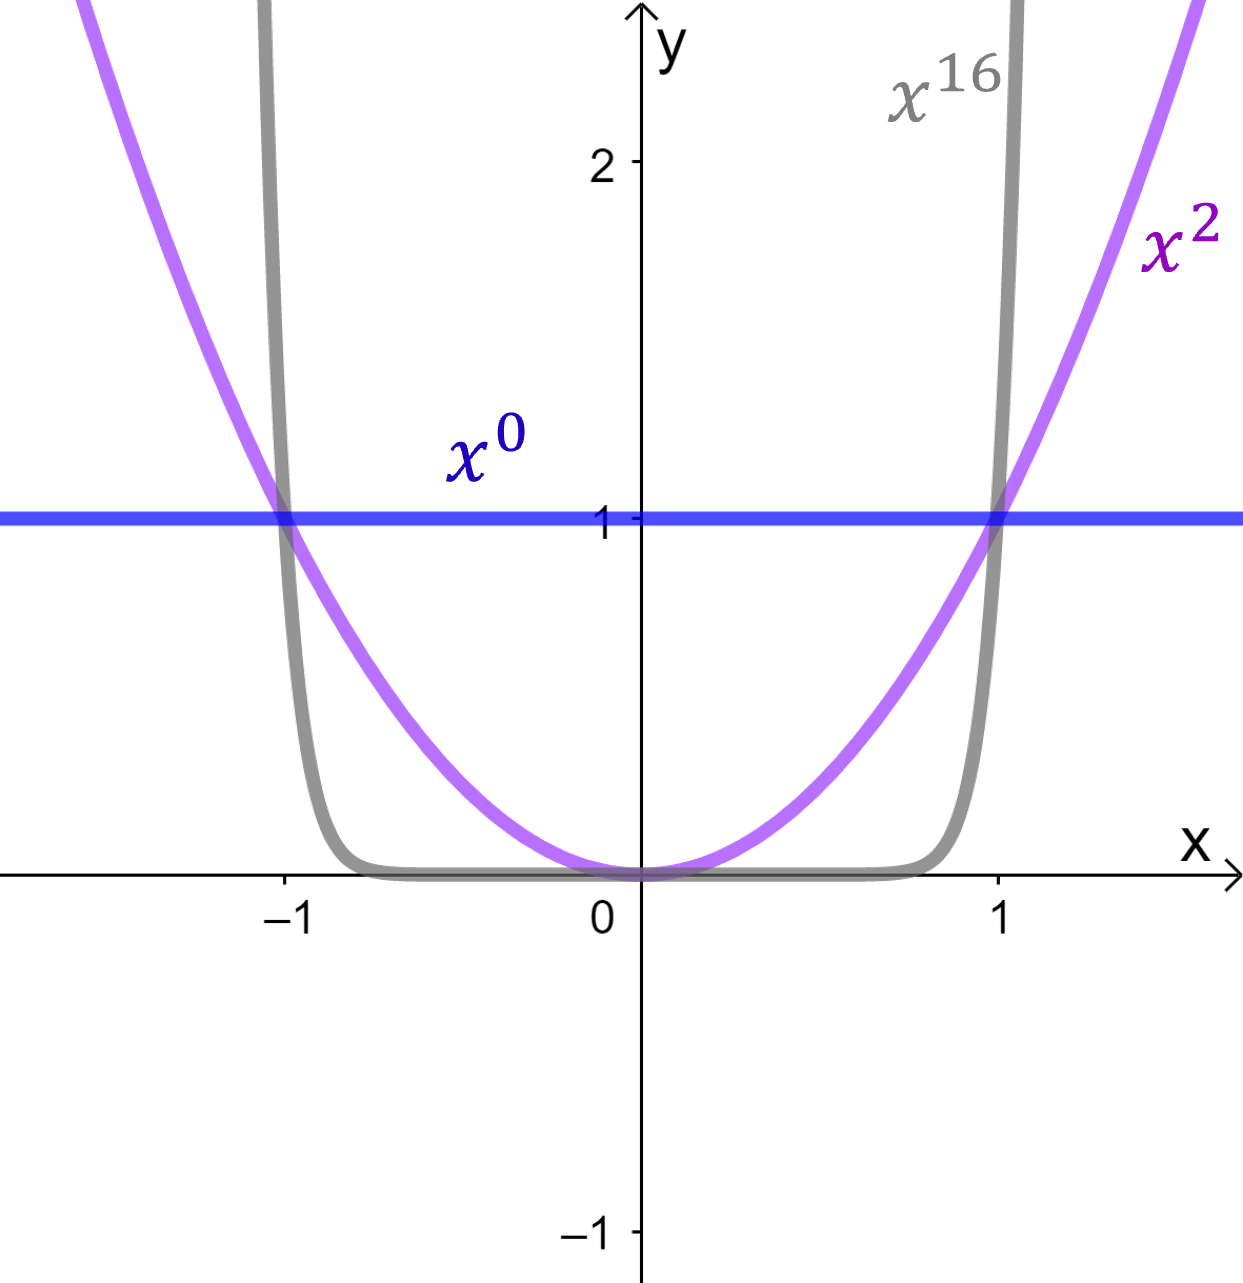
\includegraphics[width=\textwidth]{../Mathematik_1/Bilder/potenzfunktionen_gerade_exponenten.png}
	\end{minipage}
	\begin{minipage}{0.5\textwidth}
		Potenzfunktionen \[ f: \mathbb R \to [0, \infty), x\mapsto x^{2n}, \, n\in \mathbb N^+\] mit geradem Exponenten sind\ldots  
	\begin{itemize}
		\item achsensymmetrisch (gerade), also \[ f(x) = f(-x)\,,\] 
		\item auf $(-\infty, 0]$ streng monoton fallend,
		\item auf $[0,\infty)$ streng monoton steigend,
		\item auf \(\mathbb R\) \textcolor{blue}{nicht bijektiv} und damit nicht invertierbar!
	\end{itemize}
	\end{minipage}
\end{theorembox}

\begin{theorembox}{Monotonie und Symmetrie von Potenzfunktionen mit ungeradem Exponenten}{ }
	\begin{minipage}{0.35\textwidth}
	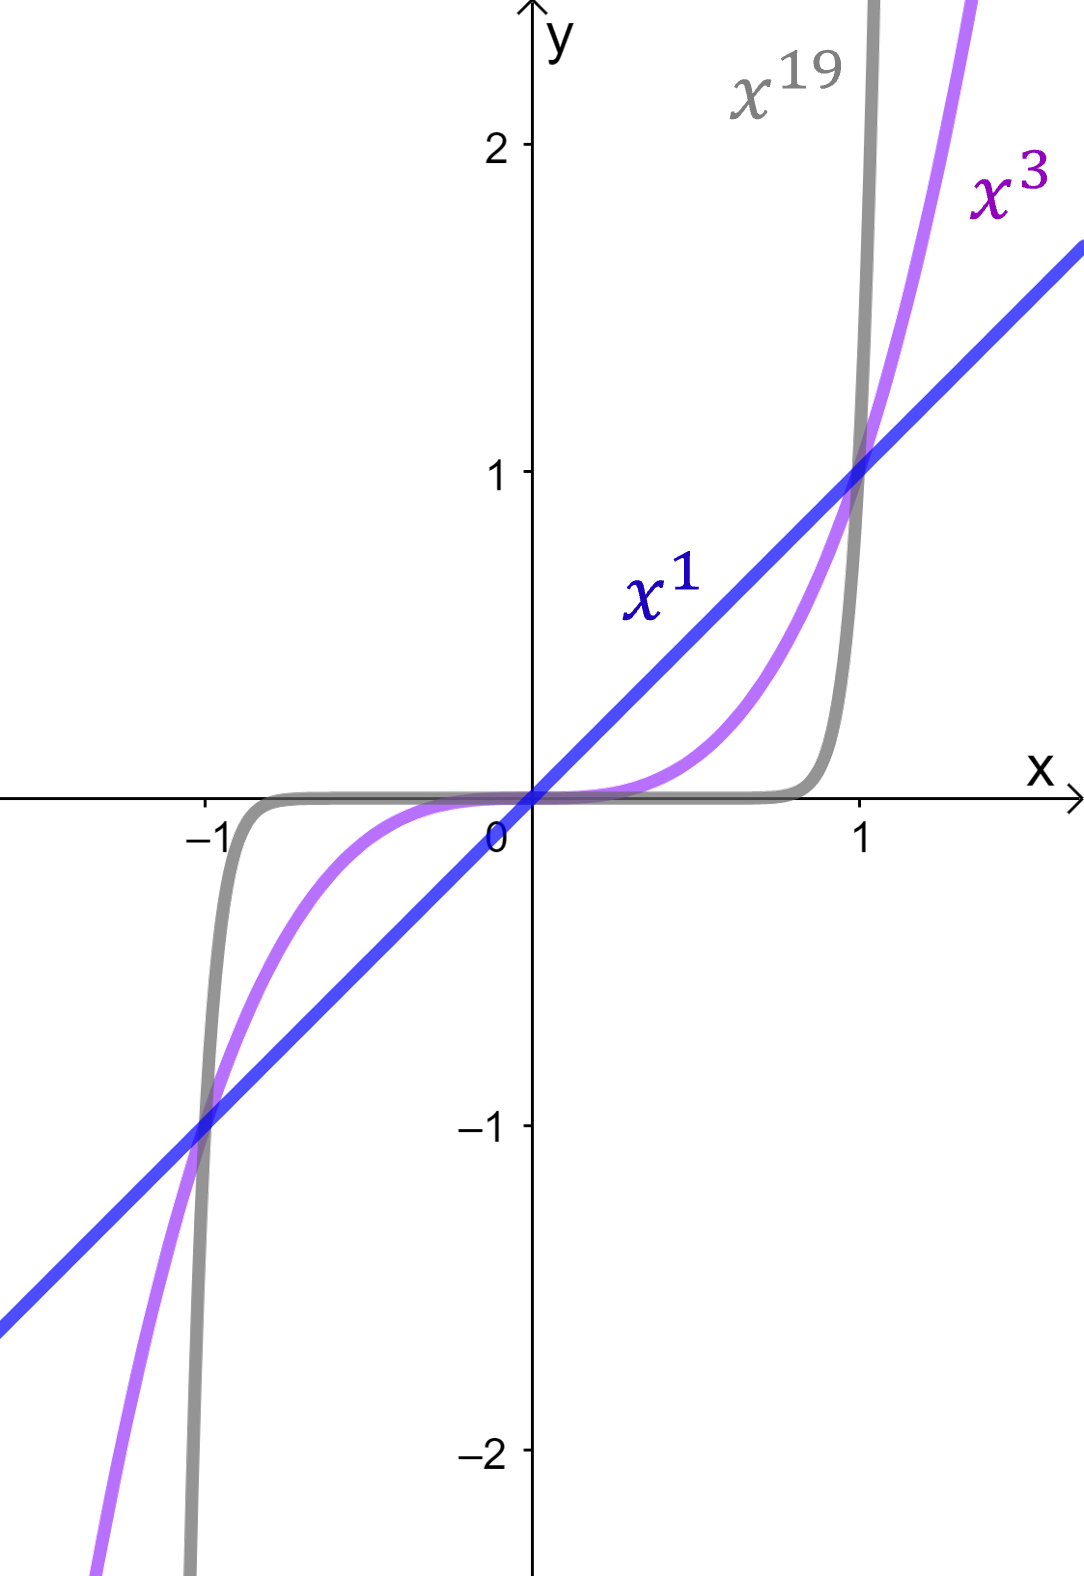
\includegraphics[width=\textwidth]{../Mathematik_1/Bilder/potenzfunktionen_ungerade_exponenten.png}
	\end{minipage}
	\begin{minipage}{0.5\textwidth}
		Potenzfunktionen \[f: \mathbb R\to \mathbb R,  x\mapsto x^{2n-1}, \, n\in \mathbb N^+\] mit ungeradem Exponenten sind \ldots
	\begin{itemize}
		\item punktsymmetrisch (ungerade), also \[f(-x) = -f(x)\,,\] 
		\item auf \(\mathbb R\) streng monoton steigend, 
		\item auf \(\mathbb R\) bijektiv und damit invertierbar.
	\end{itemize}
	\end{minipage}
\end{theorembox}

\subsection{Wurzelfunktionen}

Die Monotonie- und Injektivit�tseigenschaften der Potenzfunktionen bestimmen unmittelbar, ob und auf welchem Definitionsbereich sie umgekehrt werden k�nnen. Ihre Umkehrfunktionen f�hren zu den Wurzelfunktionen (\emph{root functions}).

Ungeradzahlige Wurzeln sind die \underline{Umkehrfunktionen}\randverweis{MA1-eigenschaften-von-funktionen} der entsprechenden Potenzfunktionen. 
\begin{exabox}{Ungeradzahlige Wurzeln}{ }

  \begin{minipage}{0.4\textwidth}
	  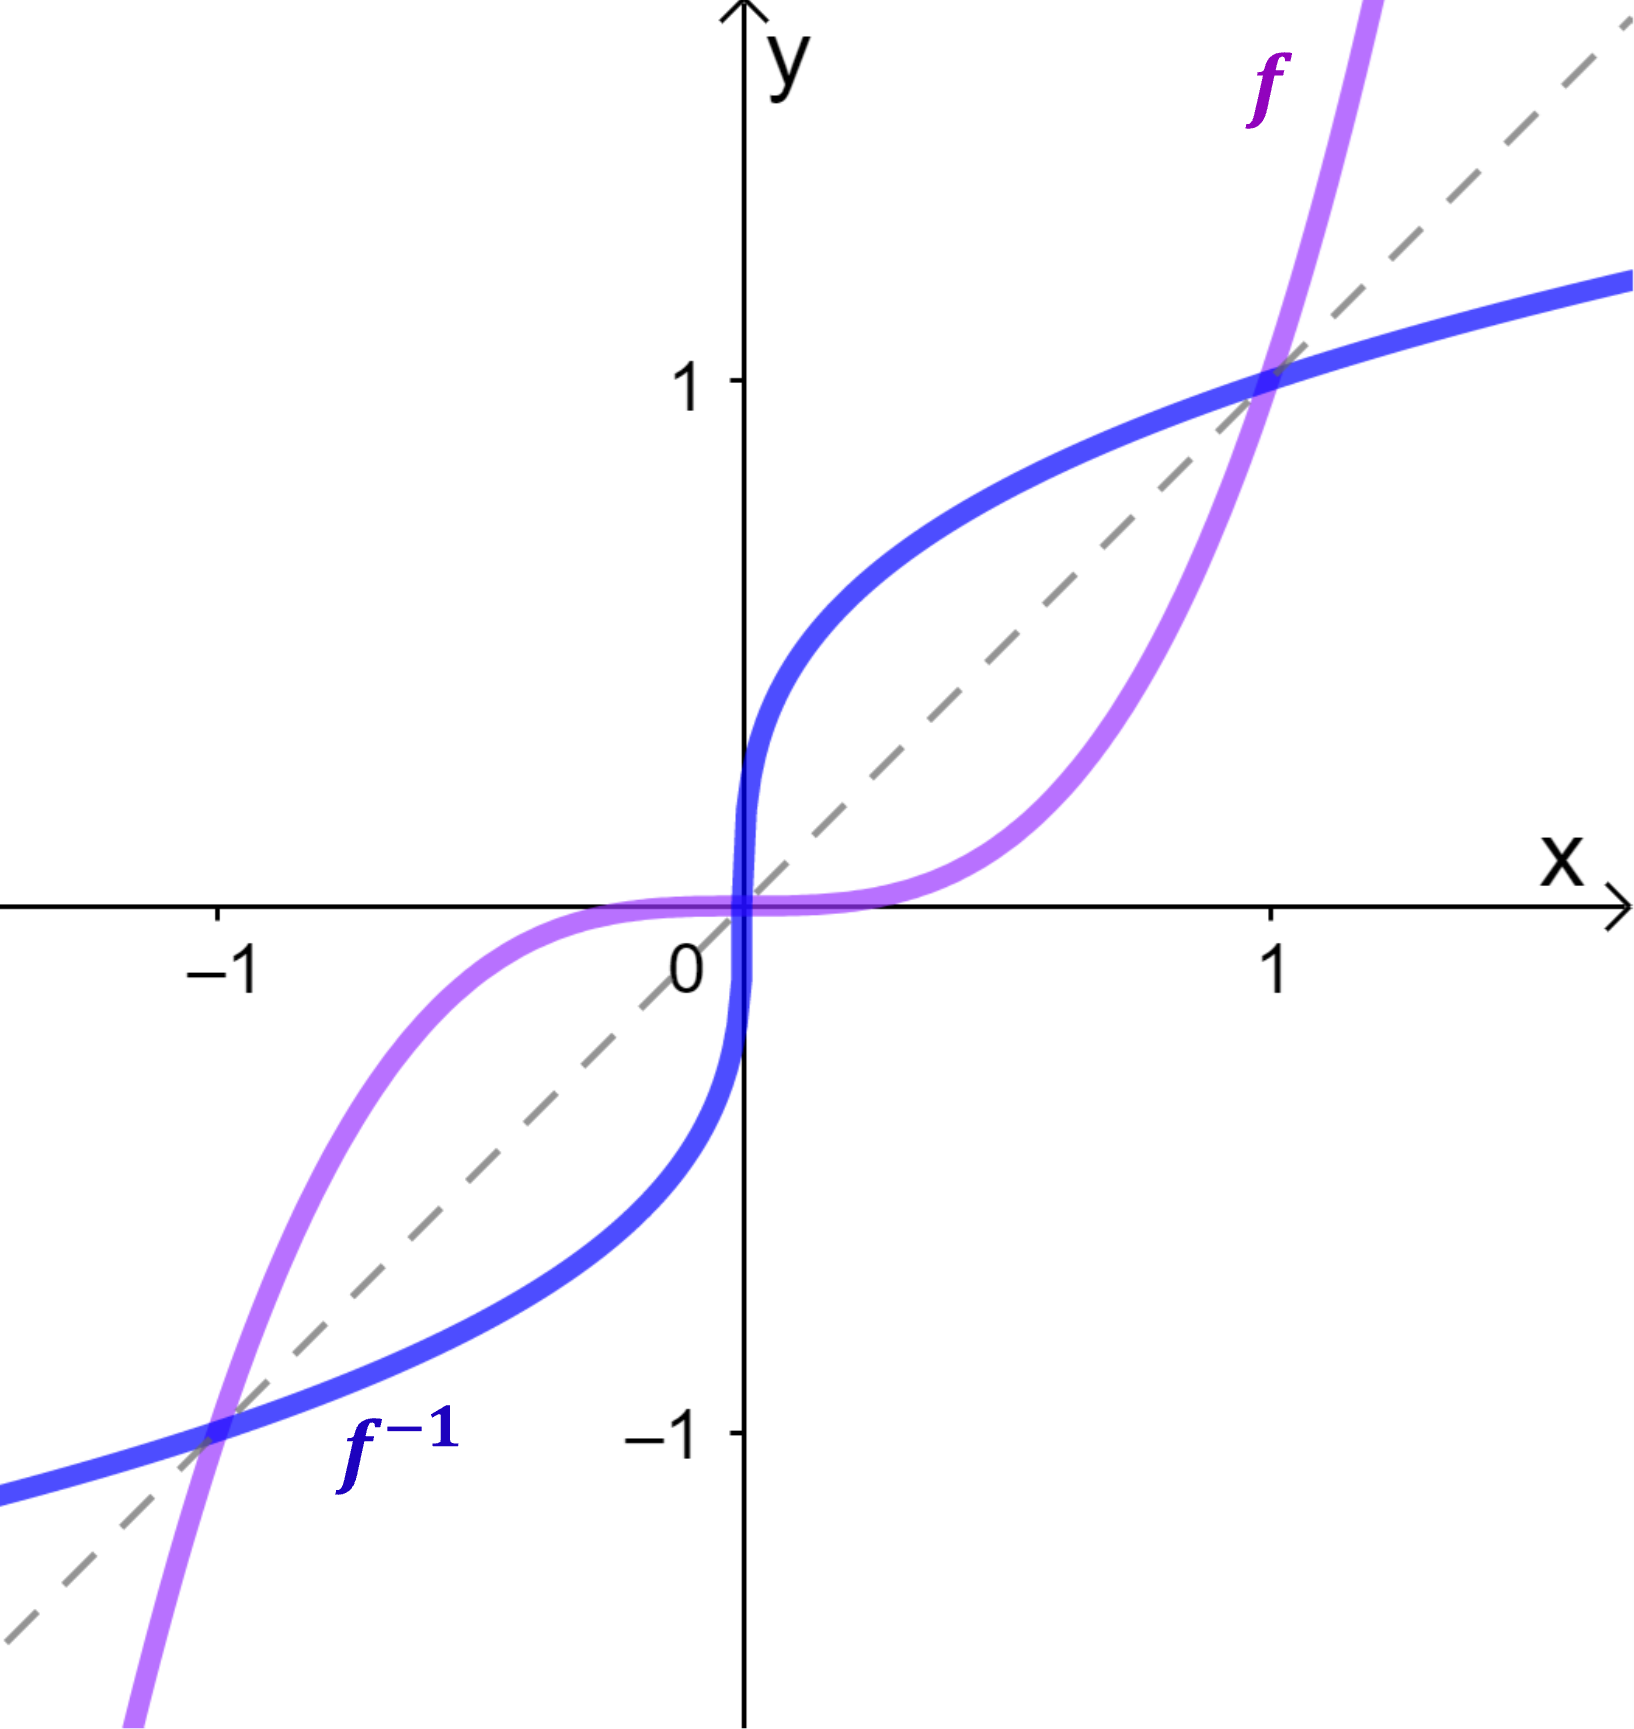
\includegraphics[width=\textwidth]{../Mathematik_1/Bilder/wurzelfunktionen_potenz_drei_dritte_wurzel.png}
\end{minipage}
\begin{minipage}{0.5\textwidth}
	\begin{itemize}
		\item \(f: x\mapsto x^3\) ist auf \(\mathbb R\) eine Potenzfunktion mit ungeradem Exponenten. 
		\item Da \(f\) auf \(\mathbb R\) streng monoton steigend und damit injektiv ist, besitzt sie auf ganz \(\mathbb R\) eine Umkehrfunktion.
		\item \(f^{-1}: x\mapsto \sqrt[3]{x}\) ist die Umkehrfunktion.
		\item "\,\textcolor{blue}{Umkehrfunktion}"\, und \textcolor{violett}{Funktion} sind an der Winkelhalbierenden gespiegelt.
		\item Ungeradzahlige Wurzeln sind f�r alle reellen Zahlen definiert. F�r negative Argumente liefern sie negative Ergebnisse.
	\end{itemize}
\end{minipage}
\end{exabox}

Potenzfunktionen mit geradem Exponenten sind auf \(\mathbb R\) nicht injektiv und besitzen daher dort keine Umkehrfunktion. Auf dem eingeschr�nkten Definitionsbereich \([0,\infty)\) sind sie dagegen streng monoton steigend und damit bijektiv auf \([0,\infty)\).

\begin{exabox}{Geradzahlige Wurzeln}{ }
  \begin{minipage}{0.4\textwidth}
	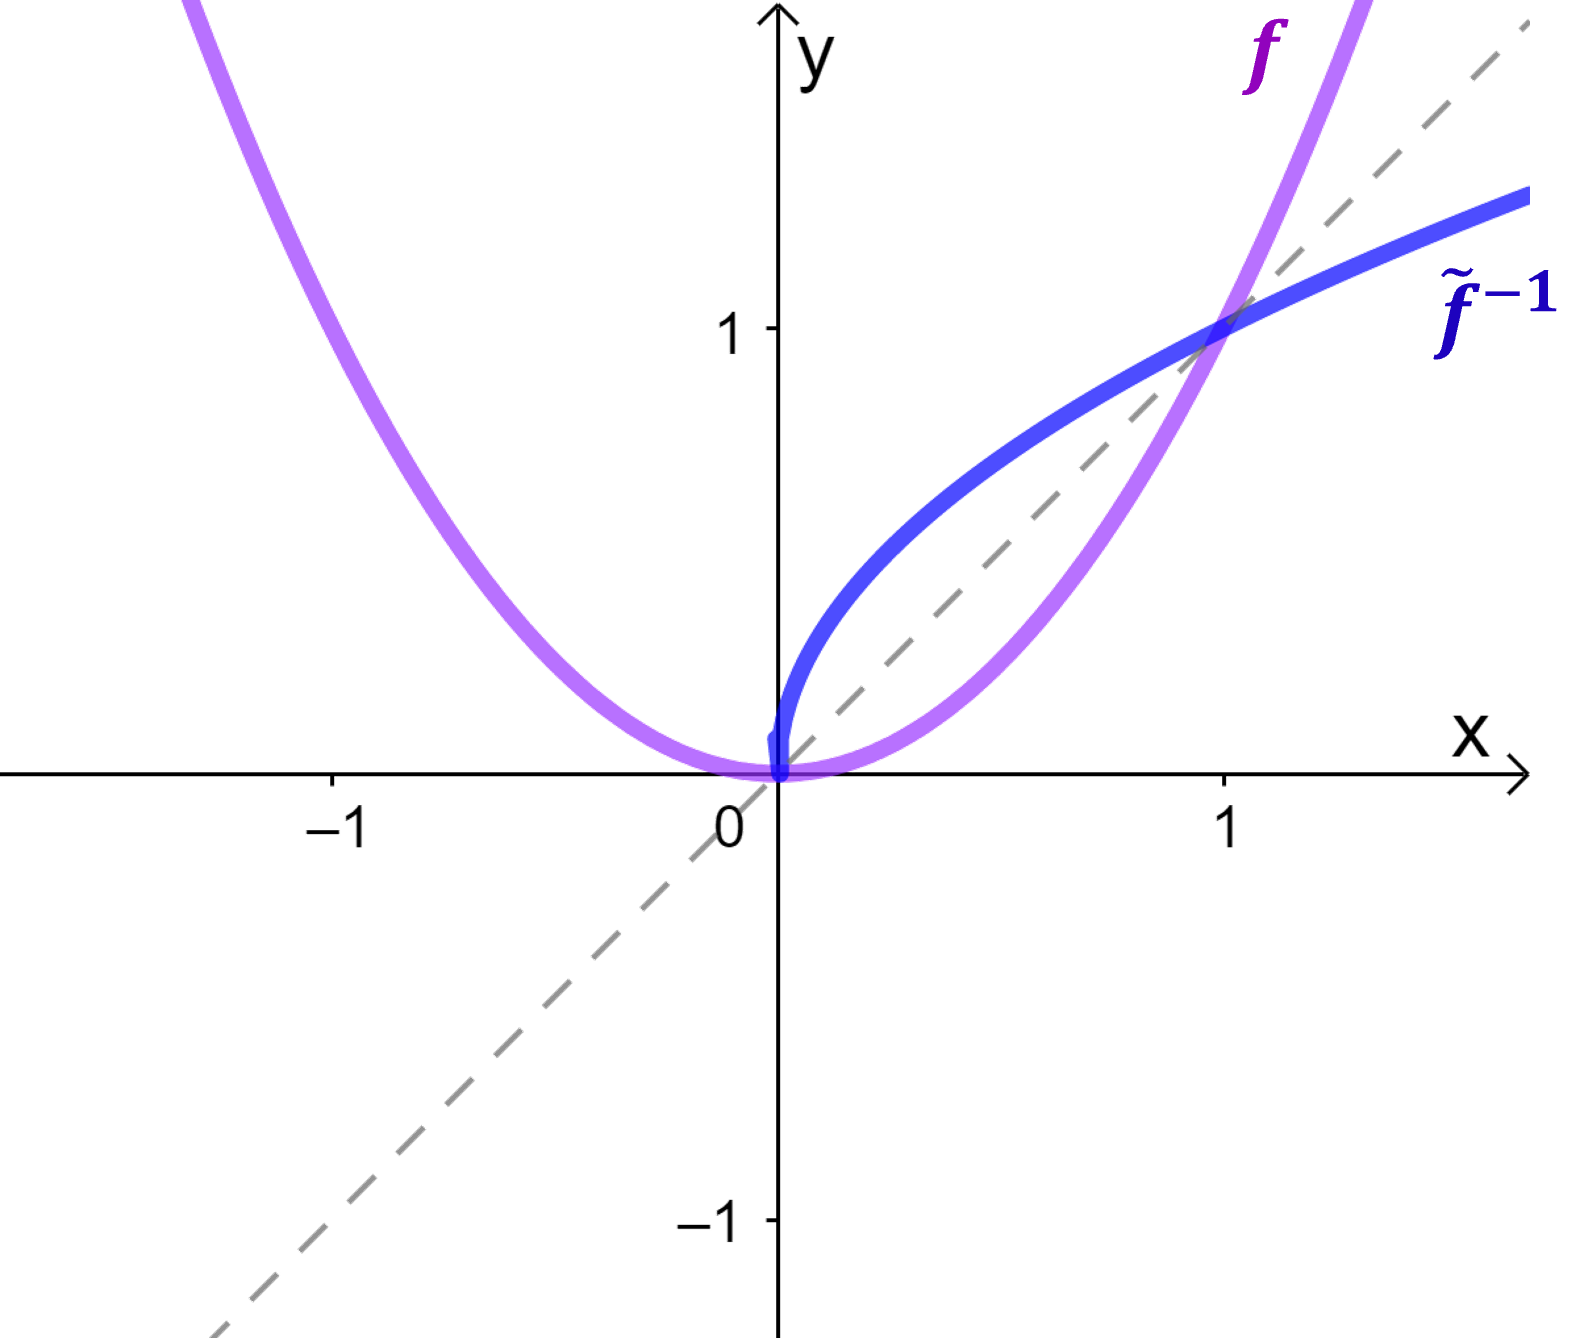
\includegraphics[width=\textwidth]{../Mathematik_1/Bilder/wurzelfunktionen_quadratfunktion_quadratwurzel.png}
\end{minipage}
\begin{minipage}{0.5\textwidth}
	\begin{itemize}
		\item \(f: \mathbb R \to [0,\infty), x\mapsto x^4\) ist auf \(\mathbb R\) eine Potenzfunktion mit geradem Exponenten. 
		\item \(f\) ist auf \(\mathbb R\) nicht invertierbar.
		\item \(\tilde f: [0,\infty) \to [0,\infty), x\mapsto x^4\) ist bijektiv und damit invertierbar.
		\item \(\tilde f^{-1}: x\mapsto \sqrt[4]{x}\) kehrt die Potenzfunktion auf \( [0,\infty)\) um.
		\item "\,\textcolor{blue}{Umkehrfunktion}"\, und \textcolor{violett}{Funktion} sind an der Winkelhalbierenden gespiegelt.

		\item Geradzahlige Wurzeln sind im Reellen nur f�r nichtnegative Argumente definiert und liefern ausschlie�liche nichtnegative Ergebnisse.
	\end{itemize}
\end{minipage}
\end{exabox}

Potenzfunktionen und Wurzelfunktionen treten h�ufig in Gleichungen auf. F�r Gleichungen der Form
\[
x^n=c
\]
h�ngt die Anzahl der reellen L�sungen entscheidend davon ab, ob der Exponent \(n\) gerade oder ungerade ist. \marginpar{Aufgaben} 

\begin{theorembox}{Gleichungen mit Potenzfunktionen}{ }
	Es sei $n\in \mathbb N^+$. Gesucht sind alle \textbf{reellen} L�sungen $x\in \mathbb R$ der Gleichung  \[ x^n = c\,.\]
	F�r $n$ gerade, also $n=2,4,6,\cdots$ besitzt die Gleichung 
	\begin{itemize}
		\item f�r $c>0$ die beiden L�sungen $x_1= - \sqrt[n]{c}$,  $x_2= \sqrt[n]{c}$,
		\item f�r $c=0$ die L�sung $x=0$, 
		\item f�r $c<0$ keine L�sung. 
	\end{itemize}
	F�r $n$ ungerade, also $n=1,3,5,7,\cdots$ besitzt die Gleichung 
	\begin{itemize}
		\item f�r $c\geq0$ die L�sung $x= \sqrt[n]{c}$,
		\item f�r $c<0$ die L�sung  $x=-\sqrt[n]{|c|}$.
	\end{itemize}
\end{theorembox}

\begin{exabox}{Gleichungen mit Potenzen}{ }

	\begin{itemize}
		\item F�r die Gleichung \(x^4=16\) ist der Exponent gerade und die rechte Seite positiv. Daher gibt es zwei reelle L�sungen:
\[
x=-\sqrt[4]{16}=-2
\qquad\text{oder}\qquad
x=\sqrt[4]{16}=2.
\]
Die L�sungsmenge ist also \( \mathbb L=\{-2,2\}\).

\item Die Gleichung \(x^3=-8 \) besitzt wegen des ungeraden Exponenten genau eine reelle L�sung:
\[
x=\sqrt[3]{-8}=-2.
\]
Damit gilt \( \mathbb L=\{-2\} \).
\end{itemize}

\end{exabox}

%Es gibt verschiedene Meinungen dazu, ob man ungerade Wurzeln aus negativen Zahlen ziehen darf oder ob doch lieber alle Wurzeln nur f�r reelle Zahlen ab $0$ aufw�rts definiert sein sollten. Mit Wolfram Alpha gibt es noch eine gr��ere �berraschung: \verb+cubic root of -8+ wird dort eine komplexe Zahl - aus gutem Grund (Hauptwert der Wurzel). 

\subsection{Verallgemeinerung der Potenzrechenregeln}

F�r das Produkt positiver ganzzahliger Potenzen $a^n$ und $a^m$ derselben Zahl $a\in \mathbb R$ gilt offensichtlich: $$a^n \cdot a^m = a^{n+m}\,.$$

Die bekannten Potenzrechenregeln sollen auch f�r allgemeinere Exponenten gelten. Dadurch ergibt sich auf nat�rliche Weise, wie Potenzen mit dem Exponenten \(0\), mit negativen ganzzahligen Exponenten und schlie�lich mit gebrochenzahligen Exponenten definiert werden m�ssen.

Damit die Potenzregel auch f�r den Exponenten \(0\) und f�r negative
ganzzahlige Exponenten erhalten bleibt, definiert man f�r \(a\neq0\)
\[
a^0:=1,
\qquad
a^{-n}:=\frac{1}{a^n},
\qquad n\in\mathbb N^+.
\]

F�r eine positive ganzzahlige Potenz $(a^n)^m$ einer positiven ganzzahligen Potenz $a^n$ einer Zahl $a \in (0,\infty)$ gilt offensichtlich:
  $$(a^n)^m = a^{n\cdot m}\,.$$

Um  diese  Regel  auf  gebrochenzahlige  Exponenten  zu  erweitern,  muss man definieren:
$$a^{\frac1n}: = \sqrt[n]{a}, \quad n\in\mathbb N^+\,.$$

Fassen wir die Rechenregeln zusammen:\marginpar{Aufgaben}

\begin{theorembox}{Rechenregeln}{ }
F�r \(a,b>0\) und rationale Exponenten \(r,s\in\mathbb Q\) gelten
\begin{align*}
(a\cdot b)^r &= a^r\cdot b^r,\\
a^r\cdot a^s &= a^{r+s},\\
(a^r)^s &= a^{rs},\\
a^{-r} &= \frac{1}{a^r}.
\end{align*}

Ein rationaler Exponent
\[
r=\frac{m}{n},
\qquad
m\in\mathbb Z,\quad n\in\mathbb N^+,
\]
wird dabei durch
\[
a^{\frac{m}{n}}
:=
\sqrt[n]{a^m}
=
\left(\sqrt[n]{a}\right)^m
\]
definiert.
\end{theorembox}


Bei der Basis \(0\) und insbesondere bei negativen Basen m�ssen die Voraussetzungen der Potenzrechenregeln sorgf�ltig beachtet werden.

\begin{exabox}{Vorsicht bei negativen Basen}{ }

	F�r \(x\geq0\) gilt \(\sqrt{x^2}=x\). F�r beliebige \(x\in\mathbb R\) muss dagegen ber�cksichtigt werden, dass die Quadratwurzel stets nichtnegativ ist. Daher gilt allgemein \( \sqrt{x^2}=|x|\).

Beispielsweise ist
\[
\sqrt{(-3)^2}
=
\sqrt9
=
3
=
|-3|
\neq -3.
\]

Die Potenzregel \( (a^n)^m=a^{nm} \) kann daher bei negativen Basen und nichtganzzahligen Exponenten nicht ohne zus�tzliche Voraussetzungen angewendet werden.

\end{exabox}
  % Potenzfunktionen und Wurzeln
\newpage
\setcounter{satz}{0} \setcounter{def}{0} \setcounter{exa}{0}  \section{Polynome}\label{MA1-polynome}

\begin{table}[H]
  \centering
  \begin{tabularx}{\textwidth}{p{0.9\textwidth} p{0.1\textwidth}}
    \toprule
	  \multicolumn{2}{c}{\textbf{�bersicht �ber Lernziele und Voraussetzungen}}\\
    \midrule
	  \textbf{Lernziele} &\\[.5\normalbaselineskip]
	  \tabitem Polynome definieren und ihren Grad bestimmen &\\
\tabitem das asymptotische Verhalten eines Polynoms aus Grad und f�hrendem Koeffizienten beschreiben &\\
\tabitem eine Polynomdivision durchf�hren &\\
\tabitem den Zusammenhang zwischen Nullstellen und Linearfaktoren erkl�ren und Polynome faktorisieren &\\
\tabitem die Vielfachheit einer Nullstelle am Verhalten des Funktionsgraphen interpretieren &\\
\tabitem quadratische Funktionen in Koeffizientenform, Scheitelpunktform und Linearfaktorzerlegung darstellen und die jeweils unmittelbar erkennbaren Eigenschaften interpretieren &\\
\tabitem die Abbildungsvorschrift eines Polynoms aus gegebenen Eigenschaften konstruieren &\\
    \midrule
	  \textbf{Voraussetzungen} \\[.5\normalbaselineskip]
	  \tabitem Grundlagen & \abschnittsverweis{MA1-mengen-und-logik}-\abschnittsverweis{MA1-aequivalenzumformungen}\\
	  \tabitem Potenzfunktionen und Wurzelfunktionen  & \abschnittsverweis{MA1-potenz-und-wurzelfunktionen}\\
    \bottomrule
  \end{tabularx}
\end{table}

\ifintegriereaufgaben \noindent �bungsaufgaben zum Thema finden Sie hier: \hyperref[MA1-polynome-aufgaben]{Aufgaben}
\vspace{0.3cm}
\hrule
 \fi

\subsection{Was ist ein Polynom?}

Eine Funktion
\[
p:\mathbb R\to\mathbb R
\]
hei�t \textbf{Polynom} (\emph{polynomial}), wenn ihre Abbildungsvorschrift die Form
\[
p(x)
=
a_n\cdot x^n+a_{n-1}\cdot x^{n-1}+\dots+a_1\cdot x+a_0
\]
mit
\[
a_0,\dots,a_n\in\mathbb R
\]
besitzt.

Ist \(a_n\neq0\), so hei�t \(n\) der \textbf{Grad} (\emph{degree}) des Polynoms. Die Zahlen
\[
a_0,\dots,a_n
\]
hei�en seine \textbf{Koeffizienten} (\emph{coefficients}).

Neben dem Grad sind insbesondere das asymptotische Verhalten und die
Nullstellen eines Polynoms von Bedeutung. Unter dem asymptotischen Verhalten
wird der typische Verlauf des Funktionsgraphen f�r betragsm��ig gro�e \(x\)
verstanden. Die Nullstellen eines Polynoms sind diejenigen \(x\in\mathbb R\),
f�r die \(p(x) = 0\) gilt.

Ist \(p\) von ungeradem Grad, so besitzt \(p\) mindestens eine reelle
Nullstelle. Anschaulich folgt dies daraus, dass die beiden Enden des
Funktionsgraphen f�r \(x\to-\infty\) und \(x\to\infty\) in entgegengesetzte
Richtungen verlaufen. Eine pr�zise Begr�ndung dieser Aussage wird sp�ter
mithilfe der Stetigkeit m�glich.

\begin{exabox}{Verhalten von Polynomen}{ }
	\begin{minipage}{0.4\textwidth}
		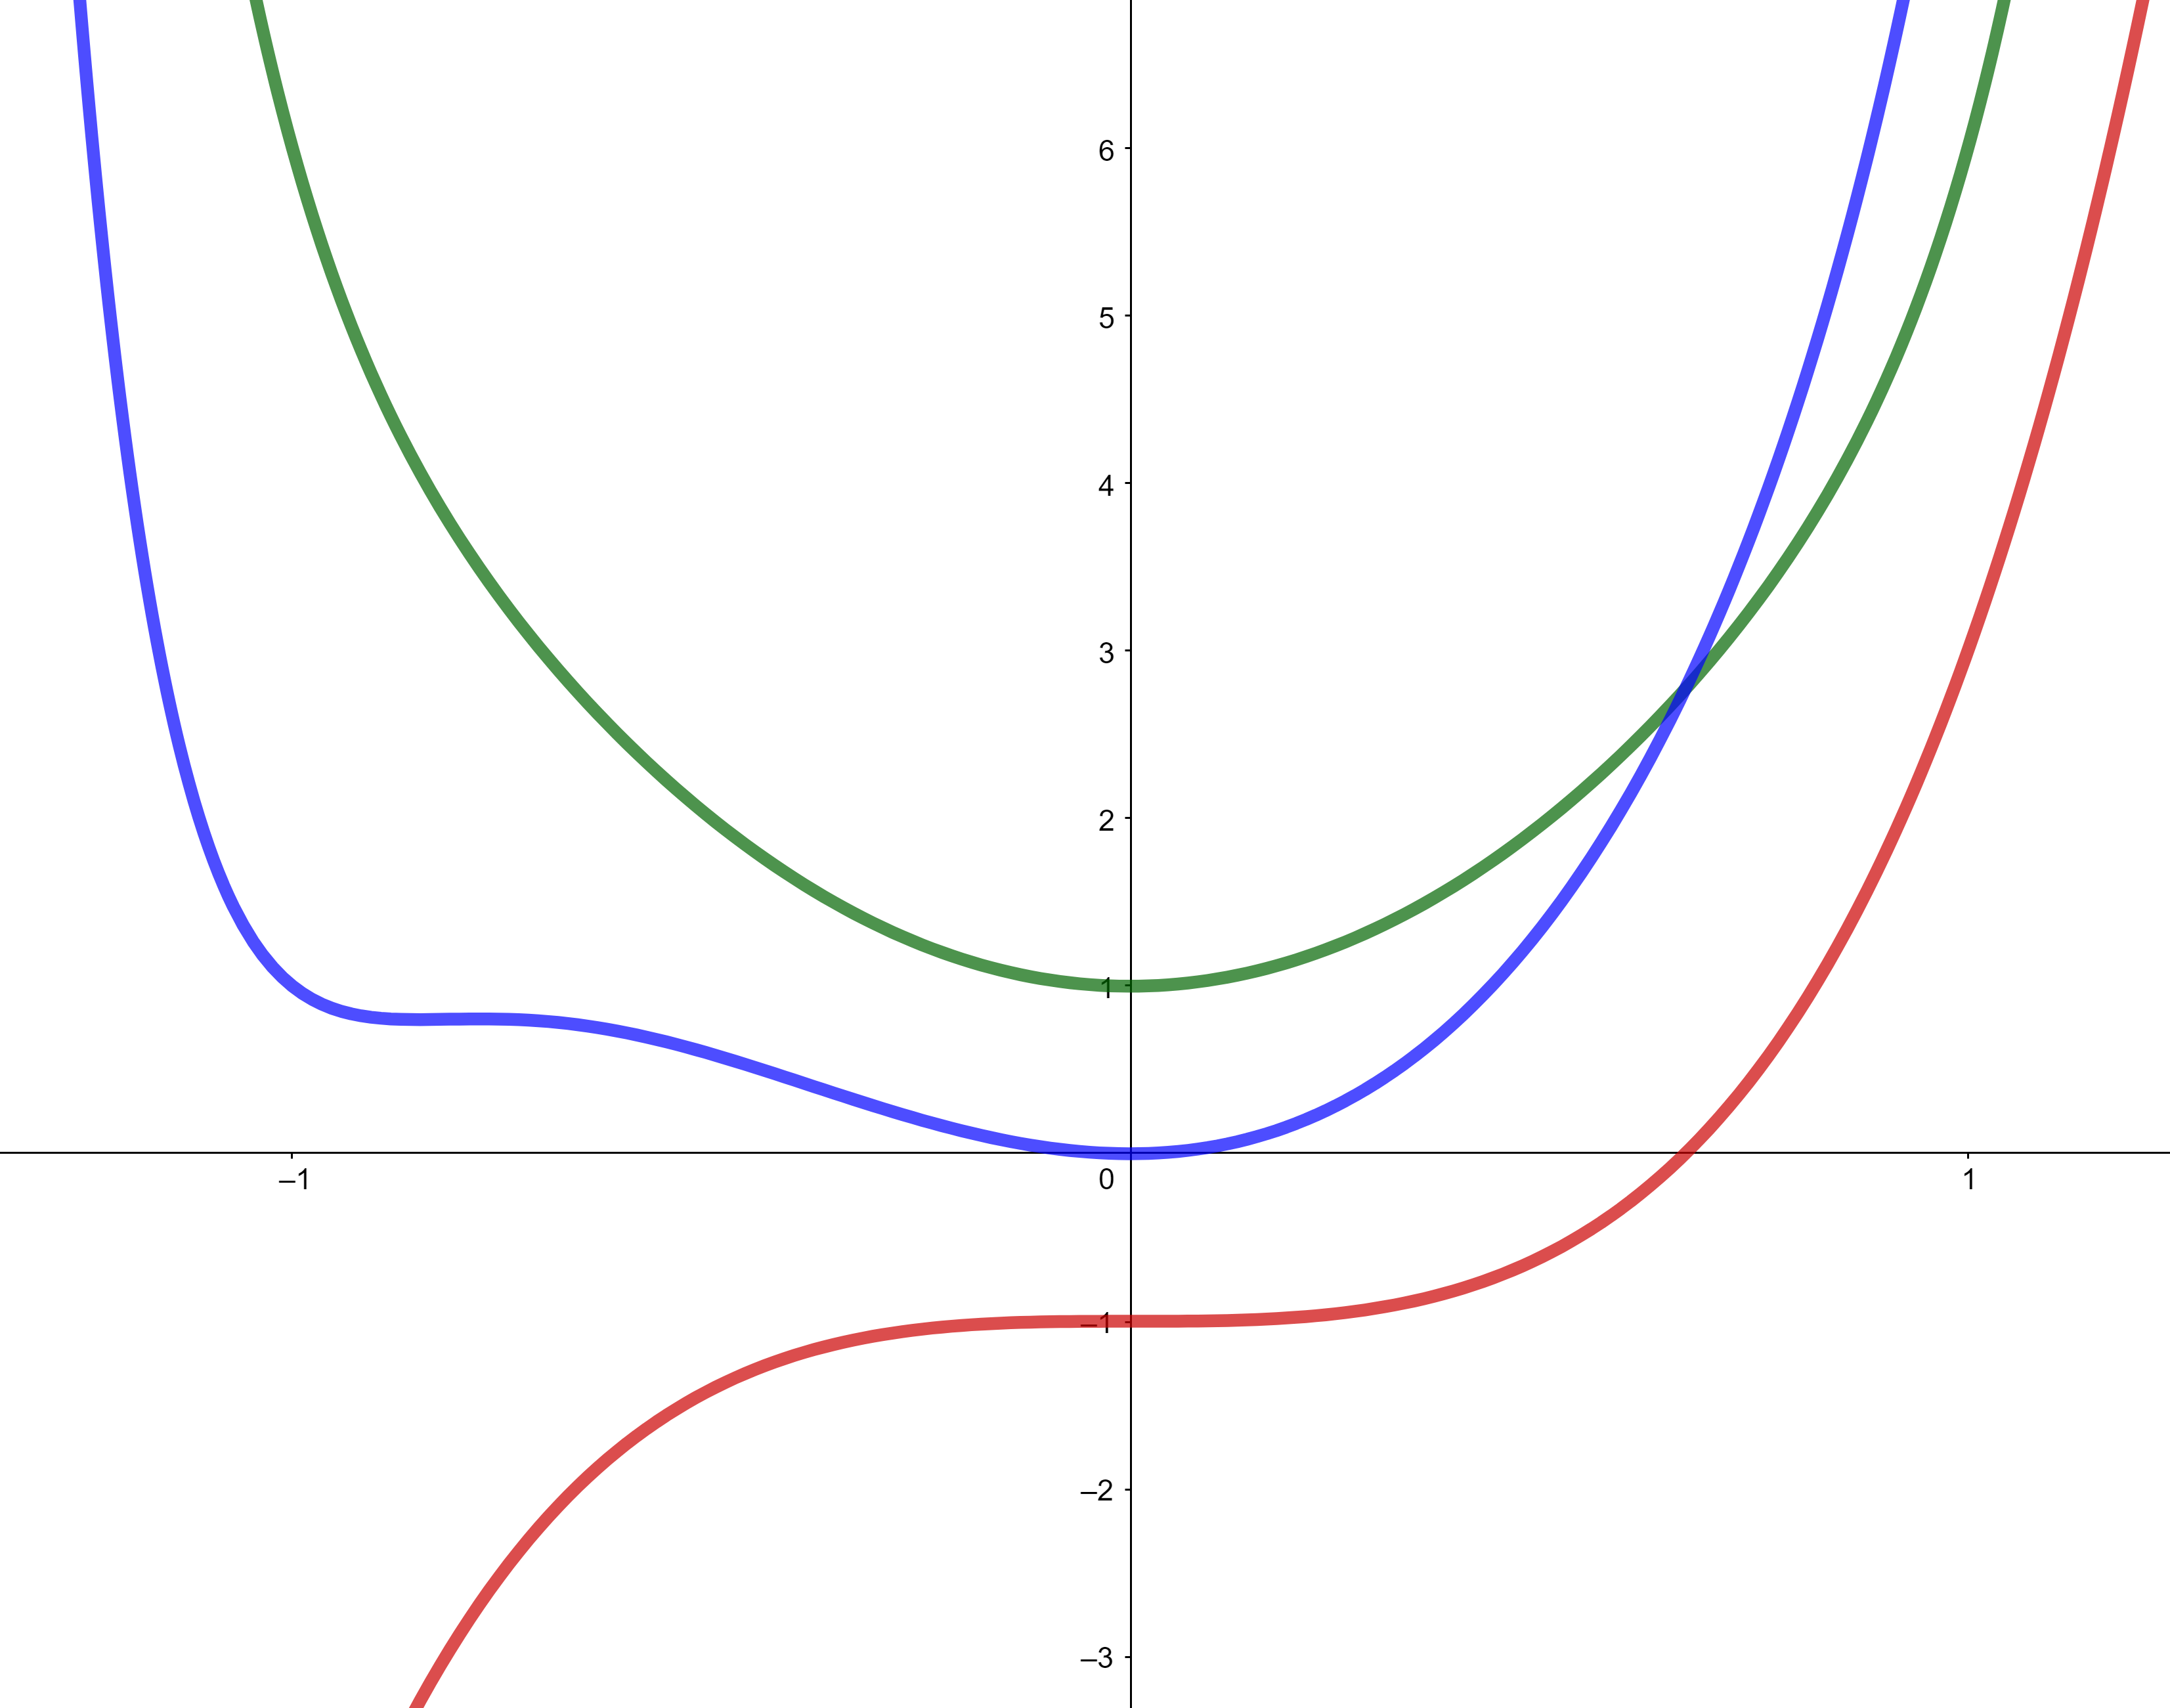
\includegraphics[width=\textwidth]{../Mathematik_1/Bilder/polynome_graphen_gerader_ungerader_grad.png}
\end{minipage}
\begin{minipage}{0.6\textwidth}
	Die Graphen links geh�ren zu folgenden Polynomen:
		\begin{itemize}
			\item \(\color{darkgreen}{h: x\mapsto x^{10}+4\cdot x^2+1}\)
			\item \(\color{red}{f: x\mapsto x^{5} +3\cdot x^3-1}\)
			\item \(\color{blue}{g: x\mapsto x^{10}+x^5+3\cdot x^3+4\cdot x^2}\)
		\end{itemize}
\end{minipage}
\end{exabox}

\noindent\textbf{Bemerkungen:}
\begin{itemize}
	\item Mit Polynomen lassen sich andere Funktionen approximieren. Die Exponentialfunktion und die trigonometrischen Funktionen k�nnen beispielsweise gut durch \underline{Polynome gen�hert werden}\randverweis{MA2-taylorreihen}:
  \begin{eqnarray*}
    e^x &\approx& 1 + x + \frac12\cdot x^2 + \frac{1}{3!}\cdot x^3 + \frac{1}{4!}\cdot x^4\,,\\
    \sin(x) &\approx& x - \frac{1}{3!}\cdot x^3\,,  \\
    \cos(x) &\approx& 1 - \frac12 \cdot x^2 + \frac{1}{4!}\cdot x^4 \,.
  \end{eqnarray*}
\item Polynome sind au�erdem beliebt als Hilfsmittel, um Messwerte zu interpolieren, beispielsweise mit einem \underline{linearen Spline}\randverweis{MA1-lineare-funktionen} oder auch mit Polynomen h�heren Grades.
	\begin{exabox}{Polynomiale Interpolation}{ }
	\begin{minipage}{0.4\textwidth}
	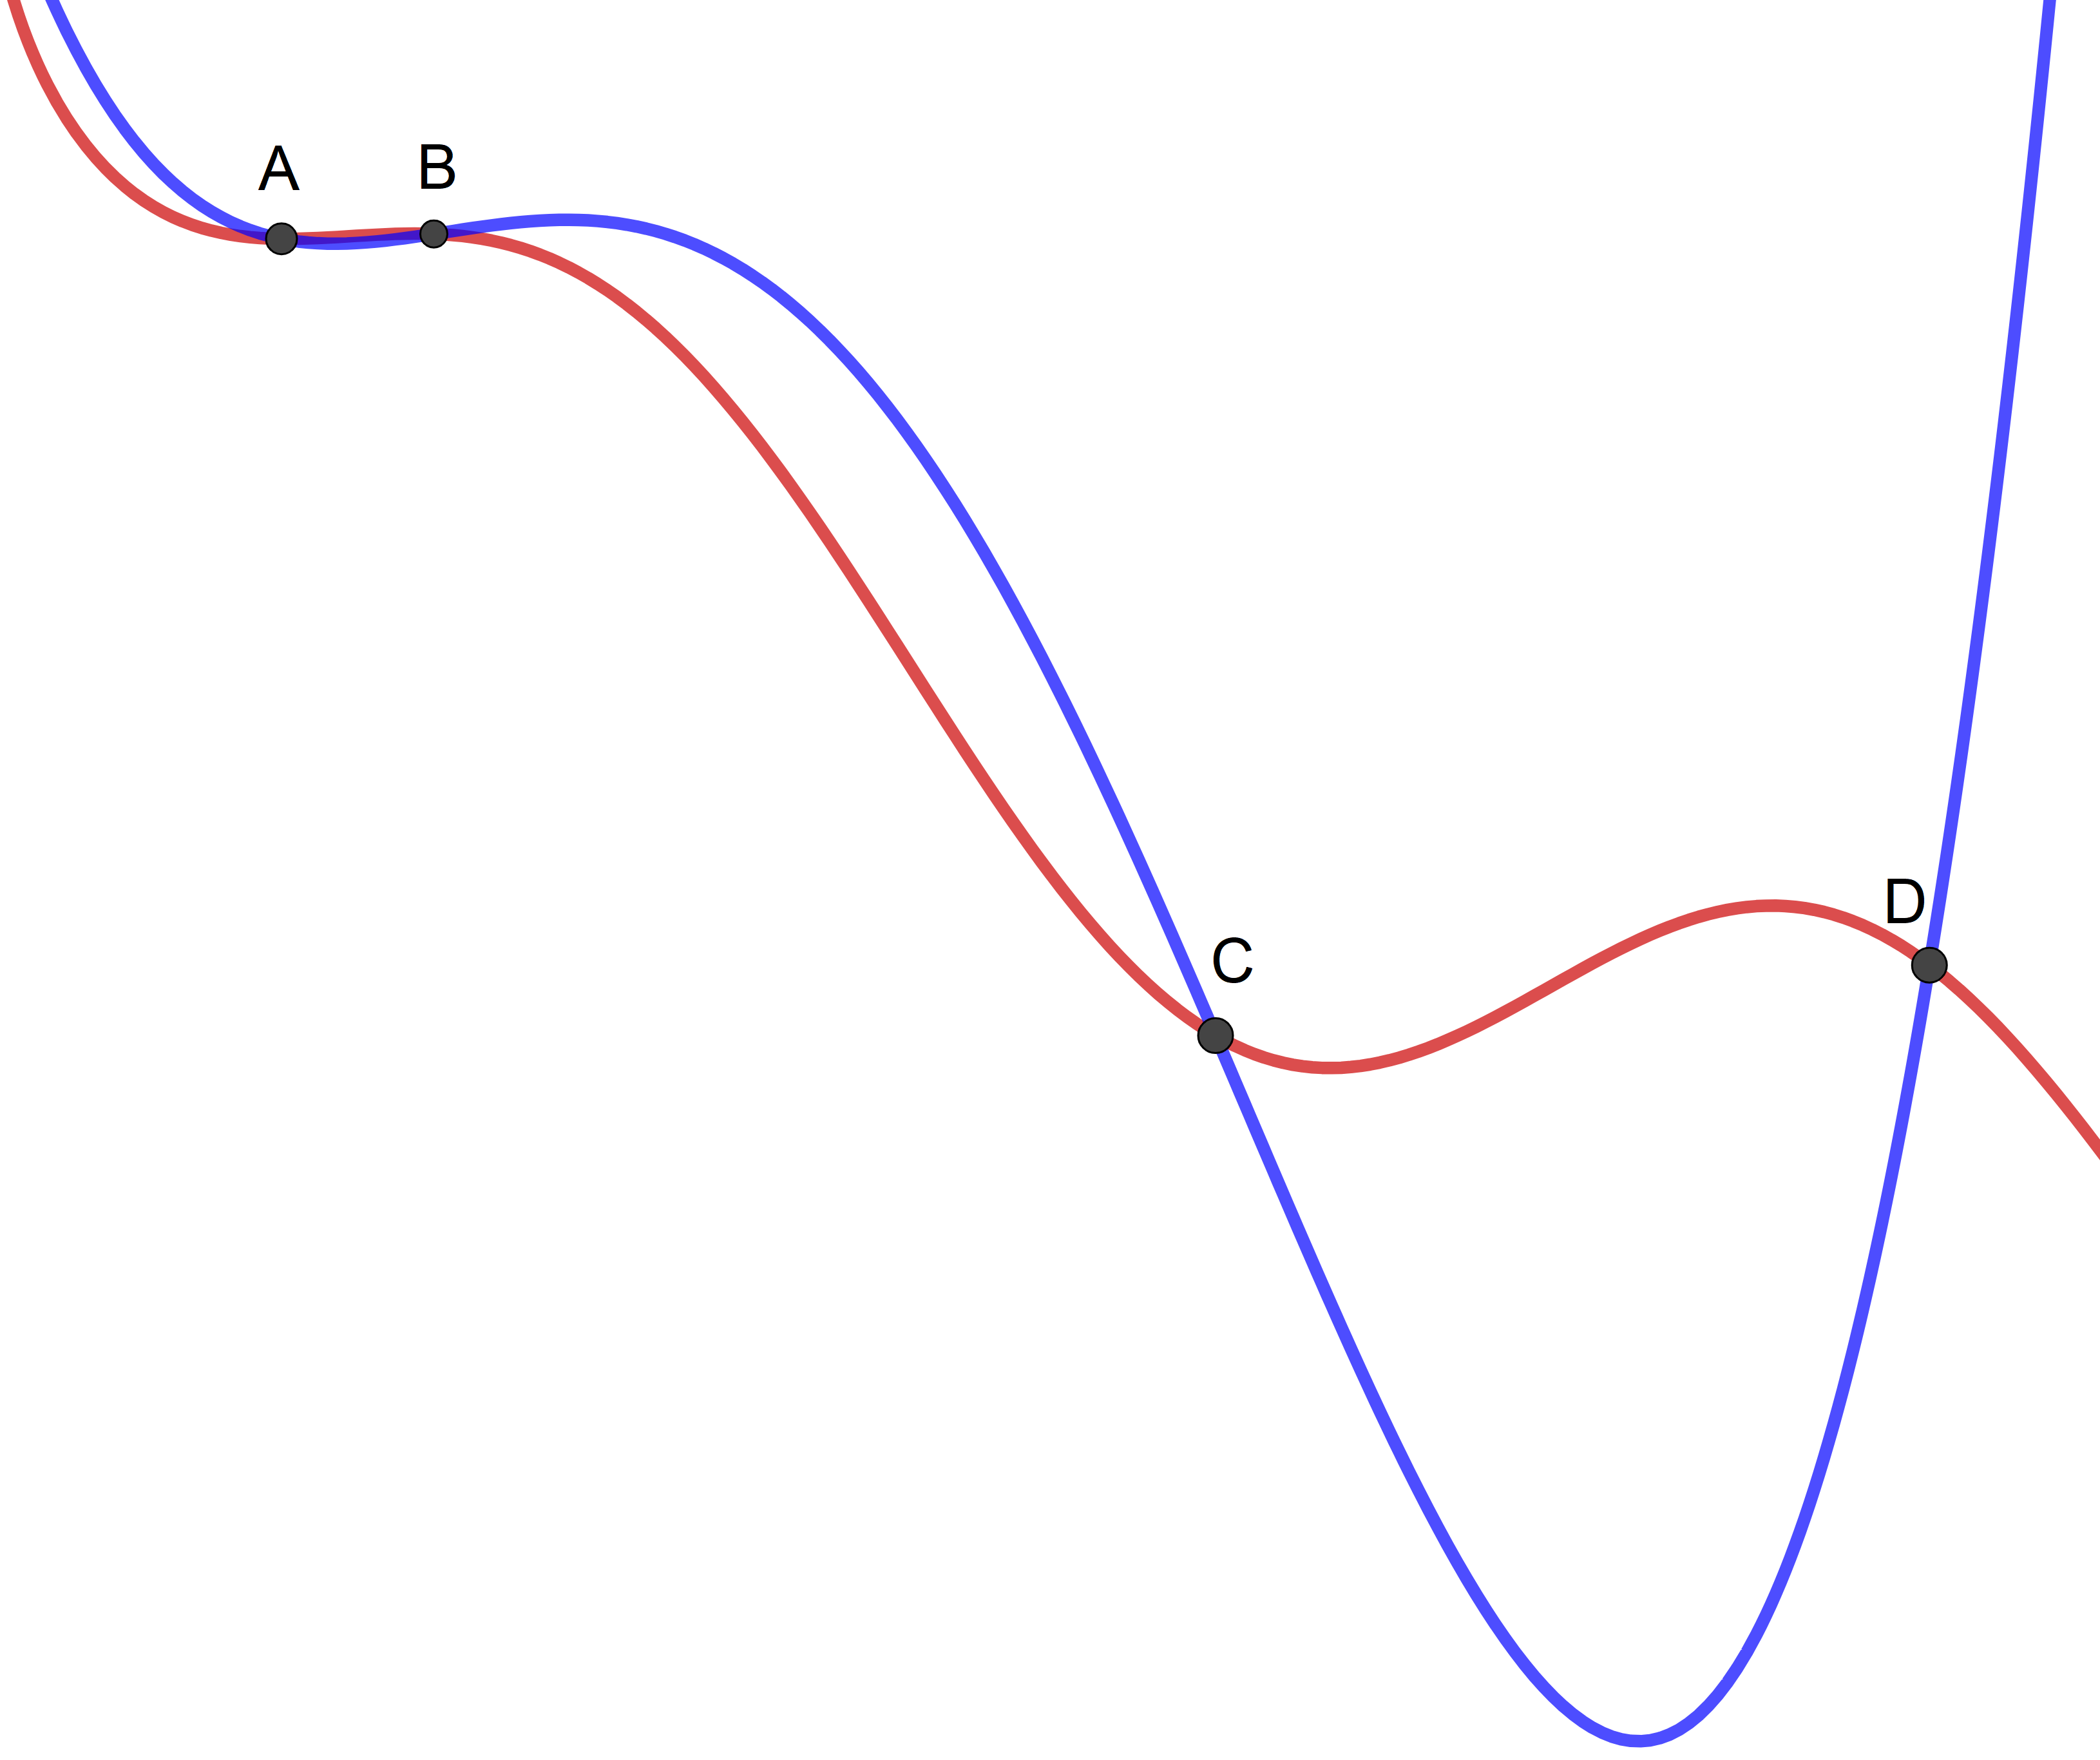
\includegraphics[width=\textwidth]{../Mathematik_1/Bilder/polynome_interpolation_funktionsvergleich.png}
\end{minipage}
\begin{minipage}{0.6\textwidth}
	\[\begin{cases} f: D_f \to \mathbb R, \;& x\mapsto \sin^2(x) - \sqrt{3\cdot x}\\
	p: \mathbb R \to \mathbb R, \;& x\mapsto \dfrac{3}{20}\cdot x^4 - \dfrac{13}{10}\cdot x^3+\dfrac{33}{10}\cdot x^2-\dfrac{319}{100}\cdot x\end{cases}\]
	\begin{itemize}
		\item[\(\Rightarrow \)] \(f\) hat den  Definitionsbereich \(D_f = [0,\infty)\).
		\item[\(\Rightarrow \)] \(p\) ist ein Polynom vierten Grades, also \(D_p = \mathbb R\).
		\item[\(\Rightarrow \)] \(p\) interpoliert \(f\) an f�nf ausgew�hlten Punkten.
		\item[\(\Rightarrow \)] asymptotisch sind \(f\) und \(p\) komplett verschieden.
		\item[\(\Rightarrow \)] die Interpolation ist eine lokale Approximation.
	\end{itemize}
\end{minipage}
		\end{exabox}

	\item Daneben treten Polynome bei der Analyse von \underline{gew�hnlichen Differentialgleichungen}\randverweis{MA2-differentialgleichungen} auf.
%Gesucht sei beispielsweise eine Funktion $f$ mit $f''-5f'+6f \stackrel{!}{=}0$. Dann kann man einen L�sungsansatz der Form $f(x) = e^{\lambda x}$ mit $\lambda\in\mathbb R\setminus\{0\}$ machen und erh�lt durch ein Einsetzen der Ableitungen $(*)$ eine polynomiale Gleichung, die es zu L�sen gilt:
%\begin{exabox}{Charakteristisches Polynom}{ }
%  $ \left.\begin{array}{rcl}
%  f(x) &=& e^{\lambda x}\\
%  f'(x) &=& \lambda e^{\lambda x}\\
%  f''(x) &=& \lambda^2 e^{\lambda x}
%\end{array}\; \right\} \;\;  \stackrel{(*)}{\displaystyle{\Rightarrow}} \;
%  \lambda^2 e^{\lambda x} - \lambda e^{\lambda x} + 6 e^{\lambda x} \stackrel{!}{=} 0 \Leftrightarrow \lambda^2 - \lambda + 6 \stackrel{!}{=} 0\,.
%  $
%\end{exabox}

	\item Die \underline{Laplace-Transformation}\randverweis{MA2-systemanalyse} transformiert komplexe Systeme in den sogenannten Bildbereich, in dem es schlussendlich um die Analyse von Polynomen geht.
	\end{itemize}

\subsection{Polynomdivision}

Polynome kann man addieren, subtrahieren und multiplizieren und erh�lt wieder Polynome\randverweis{MA1-vektorraum}:
\begin{exabox}{Polynome addieren, subtrahieren und multiplizieren}{ }
  $\begin{array}{rcl}
    \left(3\cdot x^4 + \displaystyle{\frac43}\cdot x +\sqrt{2}\right) -  \left(3\cdot x^2 + \displaystyle{\frac13}\cdot x +\sqrt{2}\right) &=&  3\cdot x^4 - 3\cdot x^2 + x\,, \\
    \left(3\cdot x + 1 \right) \cdot  \left( 2\cdot x^2 - \displaystyle{\frac13}\cdot x \right) &=& 6\cdot x^3 + x^2 - \displaystyle{\frac13}\cdot x \,.
  \end{array}$
\end{exabox}

Beim  Addieren  und  Subtrahieren  ist  der  Grad  des  Ergebnisses  maximal  so hoch  wie  der  gr��te  Grad  der  Polynome,  die  man  addiert bzw. subtrahiert. Beim Multiplizieren ist der Grad des Ergebnisses genau die Summe der Grade der beiden Polynome, die man miteinander multipliziert.

Zwei Polynome k�nnen auch dividiert werden. Das Ergebnis ist jedoch im
Allgemeinen kein Polynom. Beispielsweise ist
\[
\frac{1}{x-2}
\]
kein Polynom, da die Variable \(x\) im Nenner auftritt.

Genauso wie man aus Br�chen von nat�rlichen Zahlen einen ganzzahligen Anteil und einen \,"Rest"\, berechnet
$$\displaystyle{\frac{37}{5}} = 6 + \displaystyle{\frac{2}{5}} \quad \Rightarrow 6 + \mathrm{Rest}\; 2\,, $$
geht man bei der \textbf{Polynomdivision} vor. Hier ein Beispiel:

  \begin{exabox}{Polynomdivision}{ }
$$
\begin{array}{rcrcrcl}
	(2 x^3& +& {\color{darkgreen}{4}} x^2 & - & {\color{brown}3} x & + & {\color{blue}{3}}) : (2 x^2-x+1)= x+\frac52 + \dfrac{-\frac32 x + \frac12}{2 x^2-x+1}\\[1ex]
-(2 x^3& -& x^2 &+ &x) && \\ \hline
&&(1+{\color{darkgreen}{4}}) x^2&-&(\,1+{\color{brown}3}) x&+& {\color{blue}{3}}\,) \\[1ex]
&-&(5 x^2&-&\frac52 x &+& \frac52\,) \\\hline
 && &-&\frac32 x &+& \frac12
 \end{array}
$$
Die Polynomdivision liefert also
  \begin{eqnarray*}
          (2\cdot x^3+4\cdot x^2-3\cdot x+3) : (2\cdot x^2-x+1)= x+\frac52 + \frac{-\frac32\cdot x + \frac12}{2\cdot x^2-x+1} \quad  \Rightarrow \; x+\frac52 + \; \mathrm{Rest }\;\left( -\frac32\cdot x + \frac12\right) \,.
  \end{eqnarray*}

\end{exabox}

Ist der Grad von \(p\) mindestens so gro� wie der Grad von \(q\), so besitzt das bei der Polynomdivision \(p/q\) entstehende Quotientenpolynom den Grad
\[
\operatorname{grad}(p)-\operatorname{grad}(q).
\]
Der Rest besitzt einen kleineren Grad als der Divisor.

\subsection{Linearfaktorzerlegung}

Bereits bei linearen Funktionen wurde sichtbar, dass ein und dieselbe
Funktion unterschiedliche Darstellungen besitzen kann. Je nach gegebener
Information und Fragestellung kann dabei eine bestimmte Darstellung
besonders hilfreich sein.

F�r ein Polynom
\[
p(x)=a_nx^n+a_{n-1}x^{n-1}+\dots+a_0
\]
sind f�r die Skizze des Funktionsgraphen insbesondere die Nullstellen von
Interesse, da sie unmittelbar als Schnittpunkte mit der \(x\)-Achse
eingetragen werden k�nnen. Daraus ergeben sich drei Fragen:
\begin{enumerate}
    \item Wie viele reelle Nullstellen kann ein Polynom besitzen?
    \item Wie k�nnen diese Nullstellen bestimmt werden?
    \item Gibt es eine Darstellung des Polynoms, aus der die Nullstellen
          unmittelbar abgelesen werden k�nnen?
\end{enumerate}

Auf die Fragen gehen wir in diesem Abschnitt ein -- hier die Kurzantworten:
\begin{enumerate}
	\item Ein Polynom \(p\) vom Grad $n$ kann h�chstens $n$ verschiedene Nullstellen haben. Und zur Erinerung nochmal die �berlegungen zu Beginn des Abschnitts:
\begin{itemize}
	\item Hat \(p\) geraden Grad muss es gar keine reellen Nullstellen geben!
	\item Hat \(p\) ungeraden Grad, so gibt es mit Sicherheit zuminest eine Nullstelle!
\end{itemize}
\wennreferenzvorhanden{MA1-algebraische-gleichungen}{\item Tricks zur handschriftlichen Nullstellenbestimmung werden im Abschnitt \abschnittsverweis{MA1-algebraische-gleichungen} vorgestellt.}
\item Ja! Es gibt eine Darstellung: ist \(p\) in seine \textbf{Linearfaktoren} zerlegt, so kann man alle reellen Nullstellen sofort ablesen!
\end{enumerate}

Wie sieht die \textbf{Linearfaktorzerlegung} eines Polynoms aus? Angenommen wir kennen eine \textbf{Nullstelle} (\emph{root}) $x_1$ eines Polynoms \(p\), also $p(x_1)=0$, dann muss die Polynomdivision \( p(x) : (x-x_1)\) ohne Rest aufgehen! Angenommen, es g�be einen Rest. Dann darf der h�chstens den Grad $0$ haben, weil der Nenner den Grad $1$ hat. Ein Polynom vom Grad $0$ ist aber eine Konstante $c \in \mathbb R$. Also:
  $$p(x) : (x-x_1) = q(x) + \frac{c}{x-x_1}\,,$$
wobei $q$ ein Polynom ist, das einen Grad niedriger ist als $p$. Das Ausgangspolynom $p$ l�sst sich damit aufspalten:
$$p(x) = q(x)\cdot (x-x_1) + c \quad \land  \quad  0 \stackrel{!}{=} p(x_1) = q(x_1)\cdot \underbrace{(x_1-x_1)}_{\displaystyle{=0}} + c \; \Rightarrow \; c=0\,. $$

Wir haben also eine neue Darstellung von \(p\) gefunden, aus der die Nullstelle \(x_1\) sofort abzulesen ist:  \[ p(x_1) = 0 \;\Leftrightarrow \; p(x) = q(x) \cdot (x-x_1)\,.\] Man nennt den Vorgang "\,Abspaltung des Linearfaktors \( (x-x_1)\)".
Jede von \(x_1\) verschiedene weitere Nullstelle von \(p\) ist damit auch
eine Nullstelle von \(q\). Angenommen \(p(x_2) = 0\), dann gilt

\[ 0 = p(x_2) = (x_2-x_1) \cdot q(x_2).\]
F�r \(x_2\not= x_1\) gilt \((x_2-x_1)\not= 0\), also muss \(q(x_2) = 0\) gelten.  Auf diese Weise kann man weitere Linearfaktoren abspalten. Taucht eine Nullstelle \(n\)-fach auf, dann taucht der entsprechende Linearfaktor in der Linearfaktorzerlegung \(n\)-fach auf.

\begin{exabox}{Zweifache Nullstelle}{ }
F�r
\[
p(x)=3\cdot x^2+12 \cdot x+12
\]
gilt
\[
p(x)=3\cdot (x+2)^2.
\]
Damit ist \(x=-2\) eine Nullstelle. Da der zugeh�rige Linearfaktor
\((x+2)\) zweimal auftritt, besitzt diese Nullstelle die Vielfachheit \(2\).
\end{exabox}

  Sind also \(n\) Nullstellen, $x_1$ bis $x_n$, samt ihrer \textbf{Vielfachheiten} (\emph{multiplicity}), $k_1$ bis $k_n$, bekannt, so gelingt es mit Hilfe von Polynomdivisionen die Linearfaktorzerlegung St�ck f�r St�ck zu bestimmen:

\begin{theorembox}{Abspalten von maximal vielen Linearfaktoren}{ }
  \begin{eqnarray*}
    p(x) &=& q(x)\cdot (x-x_1) \\
    &=& \cdots \\
    &=& \underbrace{(x-x_n)^{k_n} \cdot (x-x_{n-1})^{k_{n-1}} \cdots (x-x_1)^{k_1} }_{ \displaystyle{\prod\limits_{l=1}^{l=n}  (x-x_l)^{k_l}} } \cdot \; (\textnormal{Polynom ohne reelle Nullstellen})\,.
  \end{eqnarray*}
\end{theorembox}

Die Vielfachheit der Nullstellen bestimmt �brigens, ob der Funktionsgraph die $x$-Achse schneidet oder ob er sie ber�hrt. Das folgende Beispiel zeigt das typische Verhalten des Funktionsgraphen Nullstellen unterschiedlicher Vielfachheit:

\begin{itemize}
	\item \textbf{ungerade Vielfachheit}: Graph schneidet die \(x\)-Achse,
	\item \textbf{gerade Vielfachheit}: Graph ber�hrt die \(x\)-Achse, ohne das Vorzeichen zu wechseln.
\end{itemize}

  \begin{exabox}{Graph eines Polynoms}{ }
	  \begin{minipage}{0.45\textwidth}
		  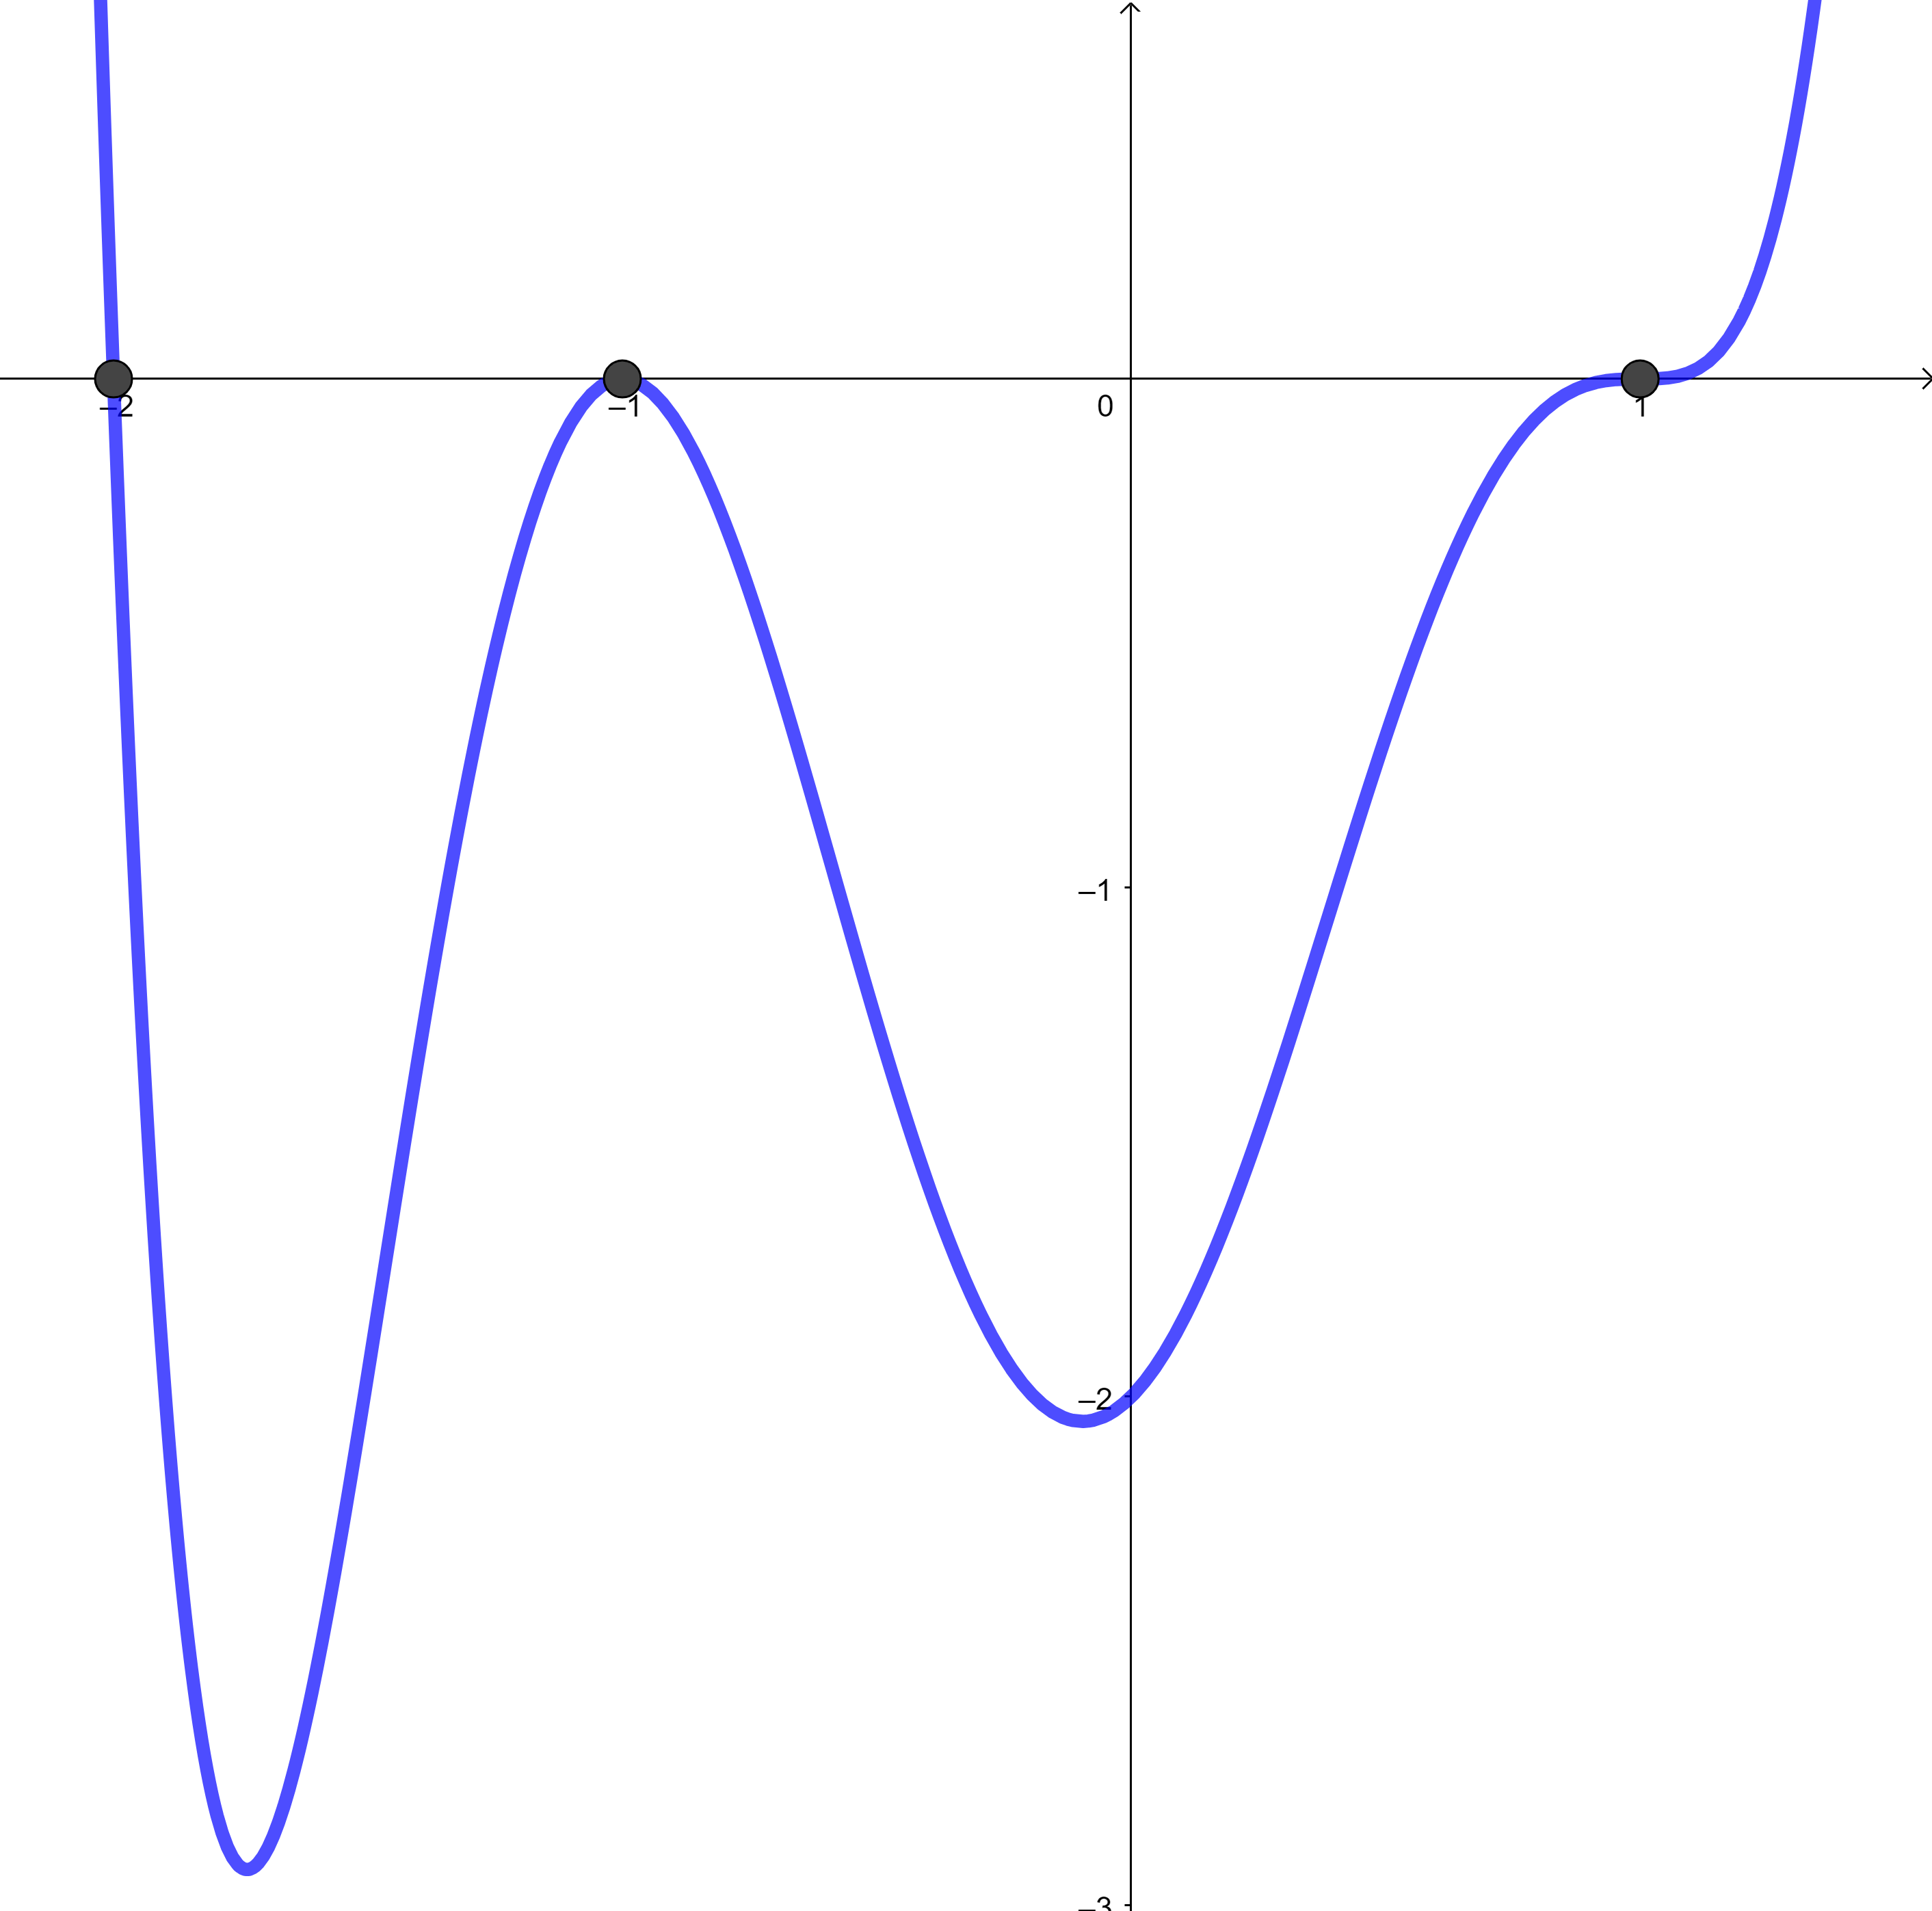
\includegraphics[width=\textwidth]{../Mathematik_1/Bilder/polynome_nullstellen_vielfachheiten.png}
\end{minipage}
	  \begin{minipage}{0.55\textwidth}
		  F�r \( p: x\mapsto (x+2)\cdot (x+1)^2\cdot (x-1)^3 \) gilt:
			  \begin{itemize}
				  \item \(p\) ist in faktorisierter Form gegeben.
				  \item \(p\) besitzt drei unterschiedliche Nullstellen: \(N_p = \{-2,-1,1\}\).
				  \item \(x=-2\) ist eine \textbf{einfache Nullstelle} \(\Rightarrow\) Achse wird geschnitten.
				  \item \(x=-1\) ist eine \textbf{doppelte Nullstelle} \(\Rightarrow\) Achse wird ber�hrt.
				  \item \(x=1\) ist eine \textbf{dreifache Nullstelle} \(\Rightarrow\) Achse wird geschnitten.
				  \item \(p\) verh�lt sich asymptotisch wie die Funktion \(x\mapsto x^6\).
			  \end{itemize}
\end{minipage}
\end{exabox}

\subsection{Parabeln}

In diesem Abschnitt geht es um Polynome zweiten Grades. Polynome zweiten Grades nennt man \textbf{quadratische Funktionen} (\emph{quadratic functions}). Ihre Funktionsgraphen sind \textbf{Parabeln}.

	\begin{itemize}
		\item Es seien $a,b,c\in \mathbb R$ mit $a\not=0$. Eine Funktion der Form \[p:\mathbb R\to \mathbb R, \; x\mapsto a\cdot x^2+b\cdot x+c \] hei�t quadratische Funktion oder Parabel in \textbf{Koeffizientenform}.

		\item Eine Parabel muss keine reellen Nullstellen haben, beispielsweise \(p(x) = x^2+1\). Aber f�r den Fall, dass es reelle Nullstellen gibt, kann man die Parabel faktorisieren.  Eine Parabel mit den Nullstellen $x_1, x_2\in \mathbb R$ (\(x_1 = x_2\) auch erlaubt) besitzt die \textbf{Linearfaktorzerlegung}
			\[p:\mathbb R\to \mathbb R, \; x\mapsto a\cdot (x-x_1) \cdot (x-x_2)\,. \]
	Ausgehend von der Koeffizientenform gilt \[ x_{1,2} = \frac{-b \pm \sqrt{b^2 - 4\cdot a\cdot c}}{2\cdot a}\,.\]

\item Die \textbf{Scheitelpunktform} macht eine andere geometrische Eigenschaft der Parabel unmittelbar sichtbar. F�r
\[
p(x)=a\cdot (x-x_S)^2+y_S
\]
ist
\[
S=(x_S,y_S)
\]
der \textbf{Scheitelpunkt} (\emph{vertex}) der Parabel. Gleichzeitig ist die vertikale Gerade
\[
x=x_S
\]
ihre Symmetrieachse.

F�r \(a>0\) ist der Scheitelpunkt das globale Minimum der Funktion, f�r \(a<0\) das globale Maximum.
\end{itemize}

\begin{exabox}{Verschiedene Darstellungen derselben Parabel}{ }

Die quadratische Funktion
\[
p:\mathbb R\to\mathbb R,
\qquad
x\mapsto x^2-4x-5
\]
ist zun�chst in Koeffizientenform gegeben:
\[
p(x)=x^2-4\cdot x-5.
\]
Aus dieser Darstellung lassen sich unmittelbar die Koeffizienten
\[
a=1,\qquad b=-4,\qquad c=-5
\]
ablesen. Insbesondere zeigt \(a>0\), dass die Parabel nach oben ge�ffnet ist.

Die Nullstellen der Parabel sind
\[
x_1=-1
\qquad\text{und}\qquad
x_2=5.
\]
Damit l�sst sich dieselbe Funktion in Linearfaktoren zerlegen:
\[
p(x)=(x+1)\cdot (x-5).
\]
In dieser Darstellung sind die beiden Nullstellen unmittelbar erkennbar, denn
\[
p(-1)=0
\qquad\text{und}\qquad
p(5)=0.
\]
Der Graph der Parabel schneidet die \(x\)-Achse daher in den Punkten
\[
(-1,0)
\qquad\text{und}\qquad
(5,0).
\]

Durch quadratische Erg�nzung erh�lt man eine dritte Darstellung:
\[
\begin{aligned}
p(x)
&=x^2-4x-5\\
&=x^2-4x+4-4-5\\
&=(x-2)^2-9.
\end{aligned}
\]
Damit liegt die Scheitelpunktform
\[
p(x)=(x-2)^2-9
\]
vor. Aus ihr k�nnen der Scheitelpunkt
\[
S=(2,-9)
\]
und die Symmetrieachse
\[
x=2
\]
unmittelbar abgelesen werden.

Die drei Ausdr�cke
\[
x^2-4\cdot x-5
=
(x+1)\cdot (x-5)
=
(x-2)^2-9
\]
beschreiben also dieselbe quadratische Funktion. Je nach Fragestellung ist jedoch eine andere Darstellung besonders hilfreich:

\[ \begin{array}{lll} \text{Koeffizientenform} &\longrightarrow& \text{Koeffizienten und �ffnung},\\[1mm] \text{Linearfaktorzerlegung} &\longrightarrow& \text{Nullstellen},\\[1mm] \text{Scheitelpunktform} &\longrightarrow& \text{Scheitelpunkt und Symmetrieachse}. \end{array} \]
\end{exabox}
  % Polynome
\newpage
\setcounter{satz}{0} \setcounter{def}{0} \setcounter{exa}{0}  \section{Algebraische Gleichungen (+)}\label{MA1-algebraische-gleichungen}

\begin{table}[H]
  \centering
  \begin{tabularx}{\textwidth}{p{0.9\textwidth} p{0.1\textwidth}}
    \toprule
	  \multicolumn{2}{c}{\textbf{�bersicht �ber Lernziele und Voraussetzungen}}\\
    \midrule
	  \textbf{Lernziele} &\\[.5\normalbaselineskip]
\tabitem algebraische Gleichungen erkennen und ihren Grad bestimmen &\\
\tabitem quadratische Gleichungen mit der allgemeinen L�sungsformel l�sen &\\
\tabitem algebraische Gleichungen geeigneter Struktur auf Gleichungen niedrigeren Grades zur�ckf�hren &\\
\tabitem f�r eine algebraische Gleichung eine geeignete L�sungsstrategie ausw�hlen &\\
    \midrule
	  \textbf{Voraussetzungen} &\\[.5\normalbaselineskip]
	  \tabitem Grundlagen & \abschnittsverweis{MA1-mengen-und-logik}-\abschnittsverweis{MA1-aequivalenzumformungen}\\
	  \tabitem Polynome, Nullstellen und Polynomdivision & \abschnittsverweis{MA1-polynome}\\
    \bottomrule
  \end{tabularx}
\end{table}

\ifintegriereaufgaben \noindent �bungsaufgaben zum Thema finden Sie hier: \hyperref[MA1-algebraische-gleichungen-aufgaben]{Aufgaben}
\vspace{0.3cm}
\hrule
\fi

\subsection{Was ist eine algebraische Gleichung?}

Eine Gleichung hei�t \textbf{algebraische Gleichung} (\emph{algebraic equation}),
wenn sie sich durch algebraische Umformungen auf eine Gleichung der Form
\[
p(x)=0
\]
mit einem Polynom \(p\) zur�ckf�hren l�sst.

Im Folgenden stehen insbesondere solche Gleichungen im Mittelpunkt, die nach Ber�cksichtigung ihres Definitionsbereichs durch �quivalenzumformungen auf eine Polynomgleichung zur�ckgef�hrt werden k�nnen.


Eine algebraische Gleichung in Polynomform wird �blicherweise so dargestellt, dass alle Terme auf einer Seite stehen und nach fallenden Potenzen von \(x\) geordnet sind: 
\[
a_n\cdot x^n+a_{n-1}\cdot x^{n-1}+\dots+a_1\cdot x+a_0=0,
\qquad a_n\neq0.
\]
Der h�chste auftretende Exponent \(n\) hei�t der \textbf{Grad} der Gleichung.  Durch Division durch den f�hrenden \underline{Koeffizienten} \randverweis{MA1-polynome} \(a_n\) erh�lt man die
\textbf{normierte Form}
\[
x^n+\frac{a_{n-1}}{a_n}\cdot x^{n-1} +\dots+\frac{a_0}{a_n}=0.
\]

Das folgende Beispiel zeigt den �bergang von einer Bruchgleichung zu einer algebraischen Gleichung in normierter Form.

\begin{exabox}{Algebraische Gleichung}{ }

Gegeben sei die Gleichung
\[
\frac{x^2+7}{x-\pi}
=
\frac{\sqrt{5}}{x^2-9}+3.
\]
Aufgrund der Nenner gilt f�r den Definitionsbereich
\[
D=\mathbb R\setminus\{-3,\pi,3\}.
\]

F�r \(x\in D\) k�nnen die Nenner durch �quivalenzumformungen beseitigt werden:
\[
\begin{array}{c rcl}
& \dfrac{x^2+7}{x-\pi} &=& \dfrac{\sqrt5}{x^2-9}+3 \\[2ex]
\Leftrightarrow& (x^2+7)(x^2-9) &=& \bigl(\sqrt5+3(x^2-9)\bigr)(x-\pi) \\[1ex]
\Leftrightarrow& x^4-2x^2-63 &=& 3x^3-3\pi x^2+(\sqrt5-27)x-\pi\sqrt5+27\pi \\[1ex]
\Leftrightarrow& x^4-3x^3+(3\pi-2)x^2+(27-\sqrt5)x -63-27\pi+\pi\sqrt5 &=&0. 
\end{array}
\]

Damit liegt eine algebraische Gleichung vierten Grades in normierter Form vor.

\medskip
\noindent\textbf{Bemerkungen:}
\begin{itemize}
    \item Die Einschr�nkung
    \[
    x\notin\{-3,\pi,3\}
    \]
    bleibt w�hrend der gesamten Umformung erhalten.
    
    \item Das Multiplizieren mit den Nennern ist nur f�r diejenigen \(x\)
    eine �quivalenzumformung, f�r die diese Nenner von null verschieden sind.
    
    \item Der f�hrende Koeffizient der erhaltenen Polynomgleichung ist bereits
    \(1\). Eine zus�tzliche Division zur Herstellung der normierten Form ist
    daher nicht erforderlich.
\end{itemize}

\end{exabox}

Eine algebraische Gleichung \(n\)-ten Grades zu l�sen bedeutet damit, die Nullstellen des zugeh�rigen \underline{Polynoms}\randverweis{MA1-polynome}  \(n\)-ten Grades zu bestimmen und anschlie�end zu pr�fen, welche dieser Nullstellen im urspr�nglichen Definitionsbereich der Gleichung liegen.
Ein Polynom \(n\)-ten Grades besitzt h�chstens \(n\) verschiedene reelle Nullstellen. Ist sein Grad ungerade, so besitzt es mindestens eine reelle Nullstelle.

%\subsection{Der Satz von Vieta}
%
%Bleiben wir bei der algebraischen Gleichung des Beispiels:
%  $$  x^4  + \displaystyle{\frac37}\cdot x^3 + \displaystyle{\frac{2+3\pi}{7}}\cdot x^2 - \sqrt{5}\cdot x + 9 = 0\,.$$
%
%  Angenommen (angenommen!), das Polynom \[ p: x\mapsto x^4  + \displaystyle{\frac37} \cdot x^3 + \displaystyle{\frac{2+3\pi}{7}}\cdot x^2 - \sqrt{5} \cdot x + 9 \] l�sst sich komplett in Linearfaktoren zerlegen, dann gibt es vier reelle Nullstellen \(x_1, x_2, x_3\) und \(x_4\) mit 
%  $$p(x) = (x-x_1) \cdot (x-x_2) \cdot (x-x_3) \cdot (x-x_4) \stackrel{!}{=} x^4  + \displaystyle{\frac37} \cdot x^3 + \displaystyle{\frac{2+3\pi}{7}} \cdot x^2 - \sqrt{5} \cdot x + 9 \,. \quad (*)$$
%  Wir haben in \((*)\) o.B.d.A.\footnote{o.B.d.A. bedeutet "\,ohne Beschr�nkung der Allgemeinheit"} die Linearfaktorzerlegung zur Darstellung von \(p\) angesetzt.\footnote{Erinnern Sie sich: dieser Ansatz ist immer dann optimal wenn es um die Nullstellen von \(p\) geht!} 
%
%  Die algebraische Gleichung haben wir gel�st, wenn wir konkrete Zahlenwerte f�r die \(x_1,\cdots,x_4\) bestimmen k�nnen und dies gelingt durch Ausmultiplizieren und \textbf{Koeffizientenvergleich}:\marginpar{Aufgaben}
%
%\begin{exabox}{Bestimmung von Nullstellen: Ansatz ausmultiplizieren und Koeffizientenvergleich}{}
%\begin{eqnarray*}  
%\lefteqn{x^4  + \displaystyle{\frac37} x^3 + \displaystyle{\frac{2+3\pi}{7}} x^2 - \sqrt{5} x + 9 \stackrel{!}{=} (x-x_1)\cdot (x-x_2)\cdot (x-x_3)\cdot (x-x_4)}\\
%  &=& x^4 - x^3\left(x_1 + x_2 +x_3+ x_4\right) + x^2\left( x_1x_2+x_1x_3+x_1x_4+x_2x_3+x_2x_4+x_3x_4 \right)\\&& - x\left( x_1x_3x_4+x_2x_3x_4+x_1x_2x_3+x_1x_2x_4 \right) + \left( x_1x_2x_3x_4\right)\\ 
%  &&\\
%  &\Rightarrow& \begin{cases}  
%	  -x_1 - x_2 - x_3 - x_4 &= \displaystyle{\frac37} \\   
%	  x_1x_2+x_1x_3+x_1x_4+x_2x_3+x_2x_4+x_3x_4  &= \displaystyle{\frac{2+3\pi}{7}} \\
%	  -x_1x_3x_4-x_2x_3x_4-x_1x_2x_3-x_1x_2x_4 &= -\sqrt{5} \\
%  x_1\cdot x_2\cdot x_3\cdot x_4 &= 9 \end{cases} 
%\end{eqnarray*}
%\end{exabox}
%
%\noindent\textbf{Bemerkungen:}
%\begin{itemize}
%	\item Unter den Voraussetzungen, dass nur reelle Nullstellen vorliegen, geht das nat�rlich auch f�r Polynome beliebigen Grades.
%	\item Das geschilderte Vorgehen zur Nullstellenbestimmung durch Koeffizientenvergleich hei�t  "\,Satz von Vieta".
%	\item Der Satz von Vieta f�hrt zu einem System nicht-linearer Gleichungen, das im Allgemeinen schwer analytisch zu l�sen ist. Eine Ausnahme sind quadratische Gleichungen.\marginpar{\small Aufgabe}
%\end{itemize}

\subsection{Quadratische Gleichungen}

Eine quadratische Gleichung kann durch quadratische Erg�nzung auf eine bereits
bekannte Gleichung mit einer zweiten Potenz zur�ckgef�hrt werden. Aus
\[
a\cdot x^2+b\cdot x+c=0,
\qquad a\neq0,
\]
folgt zun�chst durch Division durch \(a\)
\[
x^2+\dfrac ba x+\dfrac ca=0.
\]
Der Ausdruck aus \(x^2\) und \(x\) wird nun zu einem vollst�ndigen Quadrat
erg�nzt:\marginpar{Aufgaben}
  $$
  \underbrace{ x^2 + \frac{b}{a}x + \frac{b^2}{4a^2}}_{\displaystyle{ = \left(x + \frac{b}{2a}\right)^2}} + \frac{c}{a}  - \frac{b^2}{4a^2} = 0\,.
  $$
Also ist die urspr�ngliche Gleichung �quivalent zu:
$$\left(x + \frac{b}{2a}\right)^2  = \frac{\textcolor{blue}{b^2- 4\,c\cdot a}}{a^2} \,. $$
  Der Ausdruck
\[
	\Delta:= \textcolor{blue}{b^2-4\,a\cdot c}
\]
hei�t \textbf{Diskriminante} (\emph{discriminant}). Das Vorzeichen der Diskrinimante Vorzeichen bestimmt, wie viele reelle L�sungen die quadratische Gleichung besitzt.
\begin{theorembox}{L�sungsformel f�r quadratische Gleichungen}{ }
  \begin{eqnarray*}
    \begin{cases} 
      \Delta > 0 \Rightarrow x_{1,2} = \displaystyle{\frac{-b \pm \sqrt{ b^2 - 4ac}}{2a}} \quad (*)\,,\\
      \Delta = 0 \Rightarrow x_{1,2} = \displaystyle{\frac{-b}{2a}}\,,\\
      \Delta < 0 \Rightarrow \textnormal{keine reellen L\"osungen}\,.
    \end{cases}
    \end{eqnarray*}
 \end{theorembox}

 Die drei F�lle besitzen eine geometrische Interpretation.\marginpar{ \small \href{https://www.geogebra.org/m/PHfR2APJ}{GeoGebra}}
Die L�sungen der quadratischen Gleichung
\[
ax^2+bx+c=0
\]
sind genau die Nullstellen der zugeh�rigen Parabel
\[
p(x)=ax^2+bx+c.
\]
Daher schneidet die Parabel f�r \(\Delta>0\) die \(x\)-Achse in zwei Punkten, ber�hrt sie f�r \(\Delta=0\) in ihrem Scheitelpunkt und besitzt f�r \(\Delta<0\) keinen Schnittpunkt mit der \(x\)-Achse.

\subsection{Gleichungen h�herer Ordnung}

Liebt eine Gleichung h�heren Grades vor, dann ist f�r die Wahl einer L�sungsstrategie zun�chst die Struktur der Gleichung
entscheidend:

\begin{itemize}
    \item Eine quadratische Gleichung kann durch quadratische Erg�nzung oder mit der allgemeinen L�sungsformel gel�st werden.
    
    \item Ist bei einer Gleichung h�heren Grades bereits eine Nullstelle bekannt, kann der zugeh�rige Linearfaktor abgespalten und der Grad durch Polynomdivision reduziert werden.
    
    \item Tritt die Unbekannte nur in bestimmten Potenzen auf, kann eine geeignete Substitution die Gleichung auf einen niedrigeren Grad zur�ckf�hren.
\end{itemize}

\subsubsection*{Reduktion des Grades durch Polynomdivision}

\begin{exabox}{Gradreduktion durch Polynomdivision}{ }

Gegeben sei die algebraische Gleichung
\[
x^3-2\cdot x^2-5\cdot x+6=0.
\]
F�r das zugeh�rige Polynom
\[
p(x)=x^3-2x^2-5x+6
\]
sei die Nullstelle \(x_1=1\) bereits bekannt. 
Damit ist \((x-1)\) ein Linearfaktor von \(p\), und die Polynomdivision durch
\((x-1)\) geht ohne Rest auf:
\[
\begin{array}{rcrcrcl}
(x^3&-&2x^2&-&5x&+&6):(x-1)=x^2-x-6\\[1ex]
-(x^3&-&x^2)&&&&\\ \hline
&&-x^2&-&5x&+&6\\[1ex]
&&-(-x^2&+&x)&&\\ \hline
&&&&-6x&+&6\\[1ex]
&&&&-(-6x&+&6)\\ \hline
&&&&&&0
\end{array}
\]
Damit l�sst sich das Polynom schreiben als
\[
p(x)=(x-1)\cdot (x^2-x-6).
\]
Die urspr�ngliche Gleichung ist daher �quivalent zu
\[
(x-1)(x^2-x-6)=0.
\]
Der verbleibende quadratische Faktor kann weiter zerlegt werden:
\[
x^2-x-6=(x-3)\cdot (x+2).
\]
Somit gilt
\[
	p(x) = (x-1)(x-3)(x+2)
\]
Ein Produkt ist genau dann null, wenn mindestens einer seiner Faktoren null
ist. Daher ergeben sich die drei L�sungen
\[
	p(x) = 0 \Leftrightarrow x\in \mathbb L=\{-2,1,3\}.
\]

Durch das Abspalten des bekannten Linearfaktors wurde die Gleichung dritten
Grades auf eine quadratische Gleichung zur�ckgef�hrt. Allgemein kann eine
bekannte Nullstelle einer Polynomgleichung h�heren Grades auf diese Weise
genutzt werden, um den Grad der noch zu l�senden Gleichung zu reduzieren.

\end{exabox}

\subsubsection*{Reduktion des Grades durch Substitution}

\begin{exabox}{Gradreduktion durch Substitution}{ }

Gegeben sei die algebraische Gleichung
\[
x^4-5\cdot x^2+4=0.
\]
Obwohl es sich um eine Gleichung vierten Grades handelt, besitzt sie eine
besondere Struktur: Die Unbekannte \(x\) tritt nur in den Potenzen
\(x^4\) und \(x^2\) auf. Da
\[
x^4=(x^2)^2
\]
gilt, kann die Substitution \( z = x^2\) verwendet werden. Damit wird aus der Gleichung vierten Grades in \(x\) die
quadratische Gleichung in \(z\)
\[
z^2-5\cdot z+4=0.
\]
Der quadratische Term l�sst sich faktorisieren:
\[
(z-1)(z-4)=0 \Leftrightarrow 
z_1=1
\qquad\text{und}\qquad
z_2=4.
\]

Damit ist zun�chst die Gleichung in der neuen Variablen \(z\) gel�st. F�r
die L�sungen der urspr�nglichen Gleichung muss nun die Substitution \(z=x^2\)
r�ckg�ngig gemacht werden.

\[
	\left\{\begin{array}{rcl l} z_1&=&1 \Rightarrow x^2=1 \Longleftrightarrow & x=\pm1 \\
	z_2&=&4 \Rightarrow x^2=4 \Longleftrightarrow & x=\pm2\end{array}\right. 
\]
Damit besitzt die urspr�ngliche Gleichung die vier L�sungen \(\mathbb L=\{-2,-1,1,2\}.\)

Bei einer Substitution muss nach dem L�sen der vereinfachten Gleichung stets
zur urspr�nglichen Variablen zur�ckgekehrt werden. 
\end{exabox}

Nicht jede algebraische Gleichung l�sst sich mit den hier genannten Ideen
Verfahren analytisch l�sen. F�r allgemeine Gleichungen dritten und vierten
Grades existieren zwar ebenfalls geschlossene L�sungsformeln, diese sind
jedoch wesentlich aufwendiger und werden hier nicht behandelt.

F�r allgemeine algebraische Gleichungen f�nften oder h�heren Grades existiert
keine L�sungsformel, die mit der allgemeinen L�sungsformel f�r
quadratische Gleichungen vergleichbar w�re. Einzelne Gleichungen h�heren
Grades k�nnen aufgrund ihrer besonderen Struktur dennoch exakt l�sbar sein.

Ist eine exakte L�sung nicht zug�nglich oder nicht zweckm��ig, k�nnen
Nullstellen numerisch angen�hert werden. Beispiele daf�r sind das
Bisektionsverfahren und das Newton-Verfahren. Solche Verfahren werden sp�ter
im Abschnitt \underline{Numerische N�herung}\randverweis{MA1-lokale-linearitaet}
behandelt.
  % Algebraische Gleichungen (+)
\newpage
\setcounter{satz}{0} \setcounter{def}{0} \setcounter{exa}{0}  \section{Rationale Funktionen}\label{MA1-rationale-funktionen}

\begin{table}[H]
  \centering
  \begin{tabularx}{\textwidth}{p{0.9\textwidth} p{0.1\textwidth} }
    \toprule
	  \multicolumn{2}{c}{\textbf{�bersicht �ber Lernziele und Voraussetzungen}}\\
    \midrule
	  \textbf{Lernziele} &\\[.5\normalbaselineskip]
\tabitem rationale und gebrochenrationale Funktionen erkennen &\\
\tabitem Definitionsl�cken, Nullstellen und Polstellen systematisch bestimmen &\\
\tabitem hebbare Definitionsl�cken von Polstellen unterscheiden &\\
\tabitem das Verhalten f�r \(x\to\pm\infty\) und in der N�he von Polstellen untersuchen &\\
\tabitem Asymptoten gebrochenrationaler Funktionen bestimmen &\\
\tabitem gebrochenrationale Funktionen anhand ihrer charakteristischen Eigenschaften qualitativ skizzieren &\\
\tabitem eine gebrochenrationale Funktion aus gegebenen Eigenschaften konstruieren &\\[.5\normalbaselineskip]
    \midrule
	  \textbf{Voraussetzungen}& \\[.5\normalbaselineskip]
\tabitem Polynome, Nullstellen und Linearfaktorzerlegung & \abschnittsverweis{MA1-polynome}\\
\tabitem algebraische Gleichungen & \abschnittsverweis{MA1-algebraische-gleichungen}\\
    \bottomrule
  \end{tabularx}
\end{table}

\ifintegriereaufgaben \noindent �bungsaufgaben zum Thema finden Sie hier: \hyperref[MA1-rationale-funktionen-aufgaben]{Aufgaben}
\vspace{0.3cm}
\hrule
 \fi

\subsection{Was ist eine rationale Funktion?}

Eine Funktion \(f\) hei�t \textbf{rationale Funktion}
(\emph{rational function}), wenn ihre Abbildungsvorschrift in der Form
\[
f(x)=\frac{p(x)}{q(x)}
\]
mit \underline{Polynome}\randverweis{MA1-polynome} \(p\) und \(q\) und \(q\not\equiv0\) dargestellt werden kann.

Der maximale \underline{Definitionsbereich}\randverweis{MA1-funktionen} besteht aus allen reellen Zahlen, f�r die
das Nennerpolynom nicht null ist:
\[
D_f
=
\{x\in\mathbb R:q(x)\neq0\}
=
\mathbb R\setminus\{x\in\mathbb R:q(x)=0\}.
\]
Die Nullstellen des Nennerpolynoms sind die \textbf{Definitionsl�cken} der rationalen Funktion. Um Definitionsl�cken zu finden ist also eine \underline{algebraische} \underline{Gleichung}\randverweis{MA1-algebraische-gleichungen} zu l�sen.

\noindent \textbf{Bemerkungen:}
	\begin{itemize}
\item Polynome sind besonders einfache rationale Funktionen. Bei ihnen ist das Nennerpolynom eine Konstante $(\not=0)$,
\item Ist nach vollst�ndigem K�rzen der Funktion das Nennerpolynom nicht konstant, so hei�t die Funktion \textbf{gebrochenrational}.\marginpar{Aufgabe}
	\end{itemize}

Die Definitionsl�cken einer gebrochenrationalen Funktion k�nnen zu \textbf{Polstellen} f�hren.  

Eine Definitionsl�cke muss nicht notwendigerweise eine Polstelle sein.  Entscheidend ist, ob sie beim K�rzen gemeinsamer Faktoren von Z�hler und Nenner verschwindet.

\noindent{\textbf{Merke:}} Bleibt der entsprechende Linearfaktor nach vollst�ndigem K�rzen im Nenner erhalten, liegt eine \textbf{Polstelle} (\emph{pole}) vor. Verschwindet der Faktor vollst�ndig aus dem Nenner, liegt eine \textbf{hebbare Definitionsl�cke} (\emph{removable singularity}) vor.	

In der N�he einer Polstelle wachsen die Funktionswerte betragsm��ig unbeschr�nkt. Je nach \textbf{Vielfachheit} und Vorzeichen k�nnen dabei unterschiedliche Verl�ufe auftreten.  Ist nach vollst�ndigem K�rzen der Faktor
\[
(x-x_0)^k
\]
im Nenner enthalten, w�hrend der Z�hler bei \(x_0\) von null verschieden ist,
so besitzt \(f\) bei \(x_0\) eine Polstelle der Vielfachheit \(k\). F�r das Verhalten beim �berschreiten der Polstelle gilt:\marginpar{Aufgaben}
\begin{itemize}
    \item Ist \(k\) ungerade, wechselt die Funktion an der Polstelle ihr Vorzeichen.
    \item Ist \(k\) gerade, findet kein Vorzeichenwechsel statt.
\end{itemize}

%\subsection{Anwendung: $z$-Transformation}
%
%Rationale Funktionen treten vor allem auf, wenn man Filter oder Regelungsanlagen beschreibt, die R�ckkopplungen enthalten. Eines der einfachsten Beispiele daf�r sind digitale Filter (genauer gesagt, kausale lineare Filter). Hier arbeitet man mit Signalen, die mit einer festen Frequenz abgetastet werden. Sie k�nnen zueinander addiert, mit Konstanten multipliziert und um eine feste Anzahl von Abtastzyklen verz�gert werden - zum Beispiel so:
%\begin{tcolorbox}
%  Bild
%\end{tcolorbox}
%
%Jedes  Signal,  das  hier  vorkommt,  l�sst  sich  in  eine  rationale  Funktion  einer k�nstlichen Variablen $z$ �bersetzen: 
%\begin{tcolorbox}
%  Bild
%  $ x\mathrm{-Achsenabschnitt} \, z ^{-\mathrm{Nummer des Samples}} $
%  $ \mathrm{diskretes Signal} \to 1 - 1x^{-1} z^{-1} + 2 z^{-2} - 2 z^{-3} + z^{-4} $
%\end{tcolorbox}
%
%Die Funktion auf der rechten Seite nennt sich die $z$-Transformierte des Signals. Die Summe zweier Signale hat die Summe der beiden $z$-Transformierten; ein festes Vielfaches eines Signals hat das Vielfache seiner $z$-Transformierten. Verz�gert man ein Signal um $n$ Abtastzyklen, wird seine $z$-Transformierte mit $z^{-n}$ multipliziert. Ist $x(z)$ die $z$-Transformierte des Eingangssignals des Filters aus dem Beispiel und $y(z)$ die $z$-Transformierte des Ausgangssignals, findet man:
%\begin{tcolorbox}
%  $ x(z) \to  x(z) z^{-n}\,. $
%\end{tcolorbox}
%
%Die Wirkung des Filters wird also durch eine rationale Funktion beschrieben. Digitale Filter zu entwerfen, hei�t vor allem, sich solche rationalen Funktionen passend aus zu denken. Man kann nun sagen, wie das Filter auf einen Impuls Nummer des Samples 
%\begin{tcolorbox}
%\end{tcolorbox}
%
%reagiert (die sogenannte Impulsantwort):
%\begin{tcolorbox}
%\end{tcolorbox}

Es kann vorkommen, dass Nullstellen der Z�hlerfunktion auch gleichzeitig Nullstellen der Nennerfunktion sind, zum Beispiel hier:
\[f:x\mapsto \dfrac{ (x - 2)\cdot (x + 1) }{ ( x - 2) \cdot (x - 3)\cdot (x + 1)}\,.\]
K�nnen wir so eine Funktion k�rzen? Ja, aber nur unter Beibehaltung des Definitionsbereichs:
\begin{exabox}{Hebbare Definitionsl�cke und Polstelle}{ }
	\hspace{-0.3cm}\begin{minipage}{0.4\textwidth}
	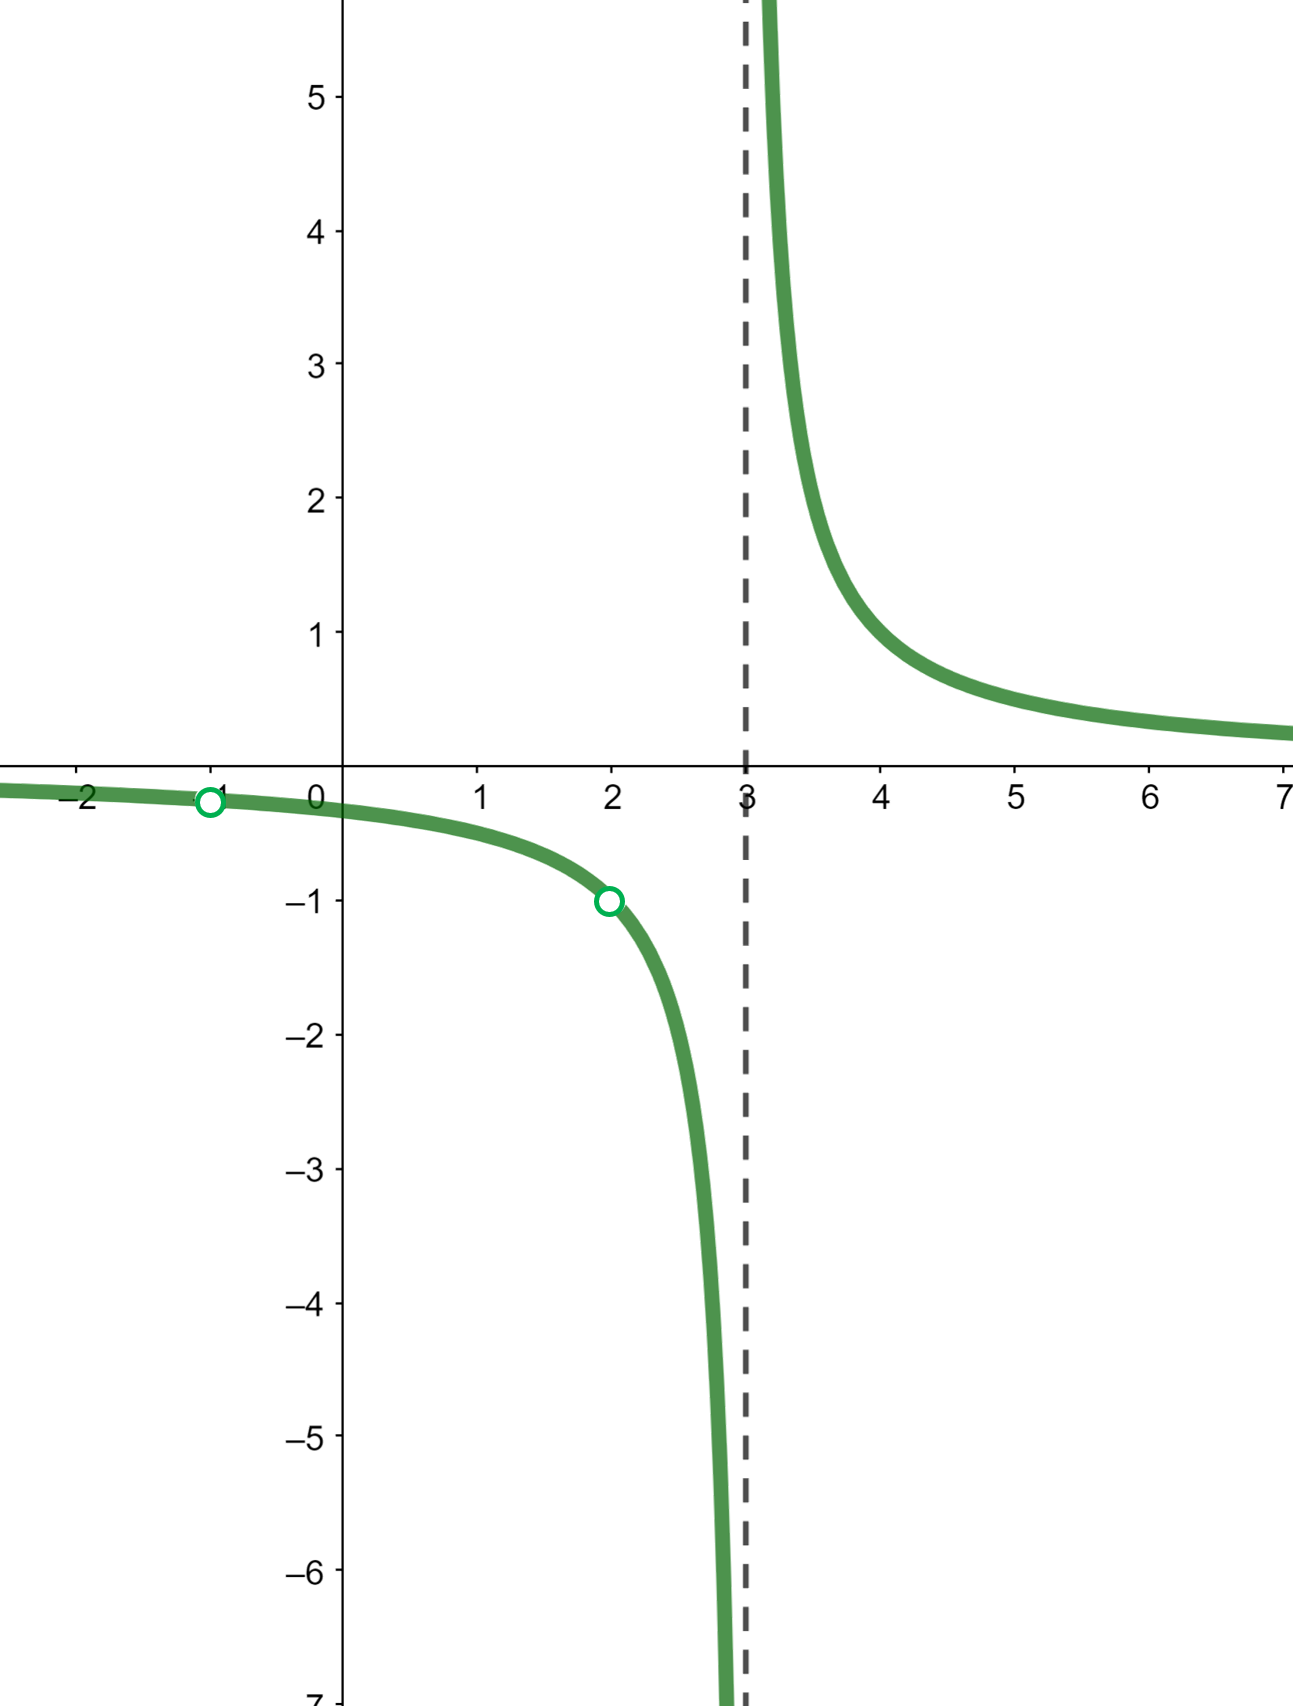
\includegraphics[width=\textwidth]{../Mathematik_1/Bilder/rationale_funktionen_hebbare_luecken_polstelle.png}
\end{minipage}
	\begin{minipage}{0.6\textwidth}
		Das Bild zeigt den Graph der Funktion \[  f: x \mapsto \dfrac{p(x)}{q(x)} = \dfrac{ (x - 2)\cdot (x+1)}{ (x - 2) \cdot (x - 3)\cdot (x + 1)}\,.\] 

		Den Funktionsverlauf von \(f\) analysieren wir wie folgt:
		\begin{itemize}
			\item Nullstellen des Z�hlers: \(N_p = \{-1, 2\}\).
			\item Nullstellen des Nenners: \(N_q = \{-1,2,3\}\).
			\item Definitionsbereich: \(D_f = \mathbb R\setminus \{ -1,2,3\} \)
			\item Nullstellen von $f$: \( N_f = \{ \} \not= N_p\)!
			\item Polstellen von \(f\): \(P_f = \{3\} \not= N_q\)!
			\item Asymptote von \(f\) f�r \(|x|\to\infty\): die \(x\)-Achse
		\end{itemize}
\end{minipage}
\end{exabox}
Die gebrochenrationale Funktion \(f\) besitzt drei Definitionsl�cken, von denen eine eine Polstelle mit Vorzeichenwechsel ist. Der Bruch ist nicht vollst�ndig gek�rzt -- die Funktionsabbildung kann noch vereinfacht werden:
		\[
			f: \mathbb R\setminus \{ -1, 2, 3\} \to \mathbb R\,, \dfrac{ (x-2)\cdot (x+1) }{(x-2)\cdot (x-3)\cdot (x+1)} = \dfrac{1}{x-3}\,. 
\]

Das Beispiel zeigt: eine Nullstelle des Z�hlerpolynoms ist nur dann eine Nullstelle der rationalen Funktion, wenn sie zum Definitionsbereich der Funktion geh�rt. Ist sie gleichzeitig eine Nullstelle des Nennerpolynoms, liegt dort zun�chst eine Definitionsl�cke vor.

Die Definitionsl�cken, die man in der gek�rzten Variante nicht mehr erkennen kann, erzeugen keine Polstellen, sondern "\,L�cher"\, im Graphen. In einer Zeichnung markiert man diese L�cher normalerweise mit einem kleinen, unausgef�llten Kringel auf dem Funktionsgraphen. 

Ist die Definitionsl�cke bei $x_0$ mehrmals vorhanden, d.h. auch nach vollst�ndigem K�rzen der Funktion ist ein \underline{Linearfaktor}\randverweis{MA1-polynome} $(x-x_0)$ im Nenner enthalten, so findet man bei $x_0$ nach wie vor eine Polstelle und kein "\,Loch"\, im Graphen. Ein Beispiel:\marginpar{Aufgaben}
\begin{exabox}{K�rzen bei einer Polstelle}{ }
	\hspace{-0.3cm}\begin{minipage}{0.4\textwidth}
	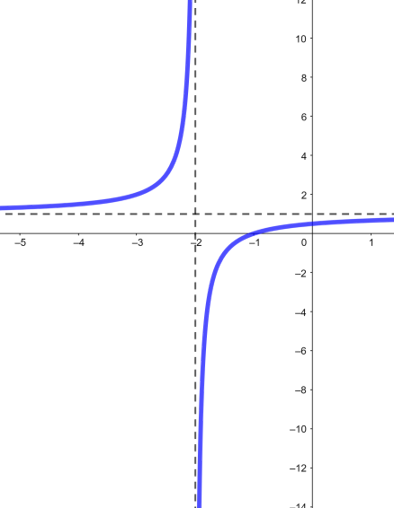
\includegraphics[width=\textwidth]{../Mathematik_1/Bilder/rationale_funktionen_polstelle_nach_kuerzen.png}
\end{minipage}
	\begin{minipage}{0.6\textwidth}
		Das Bild zeigt den Graph der Funktion \[  f: x \mapsto \dfrac{p(x)}{q(x)} = \dfrac{(x+1)\cdot (x+2)}{(x+2)^2}\,.\] 

		Den Funktionsverlauf von \(f\) analysieren wir wie folgt:
		\begin{itemize}
			\item Nullstellen des Z�hlers: \(N_p = \{-1,-2\}\).
			\item Nullstellen des Nenners: \(N_q = \{-2\}\).
			\item Definitionsbereich von \(f\): \(D =\mathbb R\setminus \{ -2\} \)
			\item Nullstellen von $f$: \( N_f = \{-1\} \not= N_p\)!
			\item Polstellen von \(f\): \(P_f = \{-2\} \not= N_q \)!
			\item Asymptote von \(f\) f�r \(|x|\to\infty\): \(x\mapsto 1\)
		\end{itemize}
	\end{minipage}	
\end{exabox}

Die gebrochenrationale Funktion \(f\) besitzt bei \(x=-2\) eine Definitionsl�cke. Obwohl ein gemeinsamer Linearfaktor gek�rzt werden kann, bleibt der Faktor \((x+2)\) einmal im Nenner erhalten. Die Definitionsl�cke ist daher eine Polstelle mit Vorzeichenwechsel.  Der Bruch ist nicht vollst�ndig gek�rzt -- die Funktionsabbildung kann noch vereinfacht werden:
		\[
			f: \mathbb R\setminus \{ -2\} \to \mathbb R\,, x\to \dfrac{ (x+1)\cdot (x+2) }{(x+2)^2} = \dfrac{x+1}{x+2}\,. 
\]

Und noch ein Beispiel
\begin{exabox}{Hebbare Definitionsl�cke ohne Polstelle}{ }
	\hspace{-0.3cm}\begin{minipage}{0.4\textwidth}
	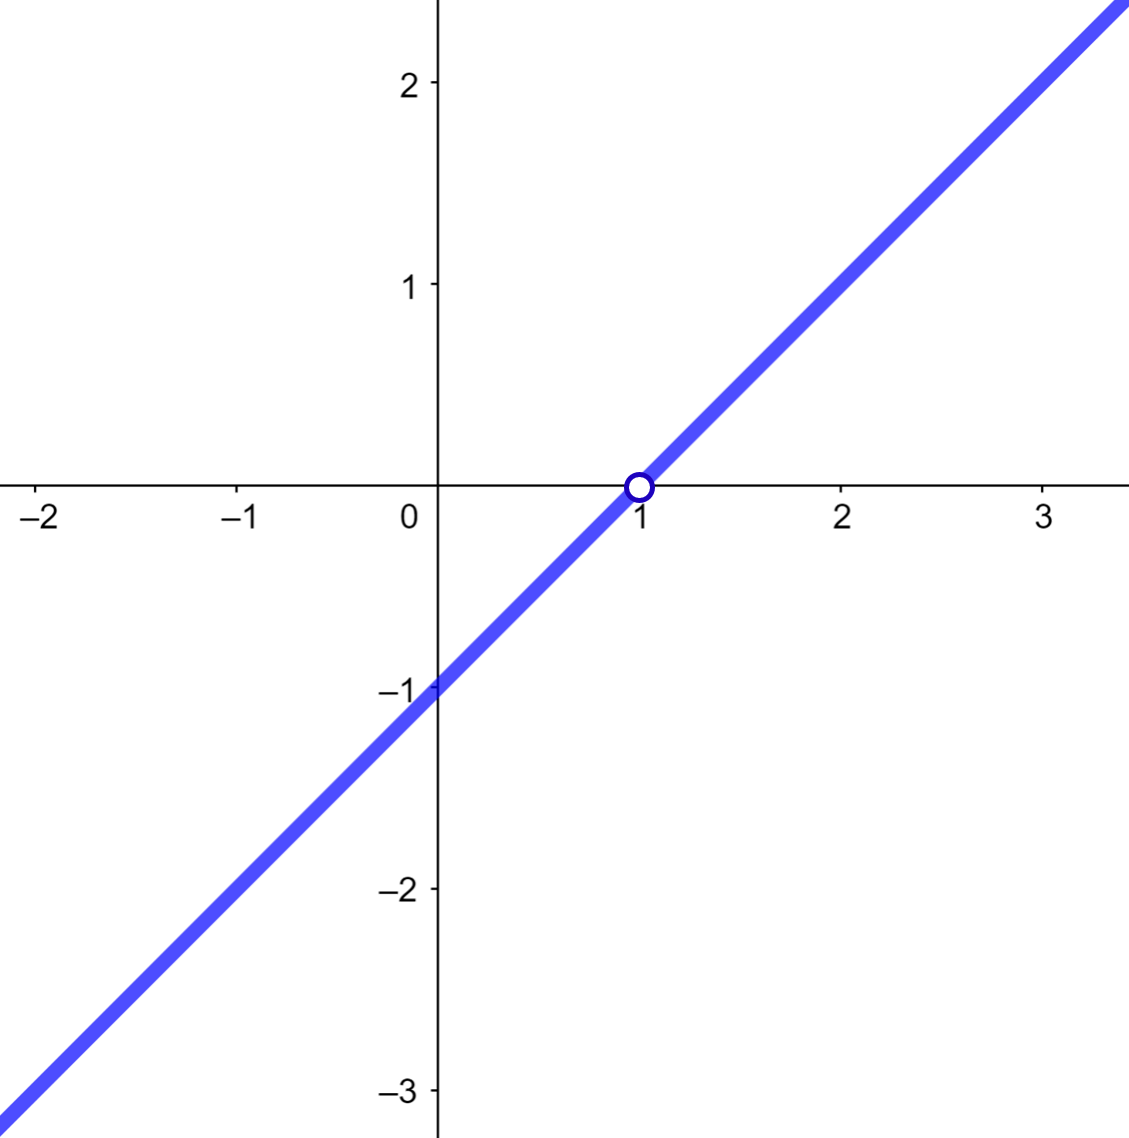
\includegraphics[width=\textwidth]{../Mathematik_1/Bilder/rationale_funktionen_gerade_hebbare_luecke.png}
\end{minipage}
	\begin{minipage}{0.6\textwidth}
		Das Bild zeigt den Graph der Funktion \[ f: x \mapsto \dfrac{p(x)}{q(x)}= \dfrac{ (x-1)^2}{(x-1)}\,.\]

		Den Funktionsverlauf von \(f\) analysieren wir wie folgt:
		\begin{itemize}
			\item Nullstellen des Z�hlers: \(N_p = \{1\}\).
			\item Nullstellen des Nenners: \(N_q = \{1\}\).
			\item Definitionsbereich von \(f\): \(D= \mathbb R\setminus \{ 1\} \)
			\item Nullstellen von $f$: \( N_f = \{\}\)!
			\item Polstellen von \(f\): \(P_f = \{\} \)
		\end{itemize}
		
\end{minipage}
\end{exabox}
		Die gebrochenrationale Funktion \(f\) besitzt eine Definitionsl�cke, keinen Pol und keine Nullstelle. Der Bruch ist nicht vollst�ndig gek�rzt -- die Funktionsabbildung kann noch vereinfacht werden:
		\[
			f: \mathbb R\setminus \{ 1\} \to \mathbb R\,, \dfrac{ (x-1)^2}{(x-1)} = x-1\,. 
\]

\noindent\textbf{Bemerkung:}
Beim K�rzen einer rationalen Funktion bleibt der urspr�ngliche Definitionsbereich erhalten. Eine durch K�rzen verschwundene Definitionsl�cke wird dadurch nicht zu einem Element des Definitionsbereichs.  

\subsection{Asymptoten f�r \(|x|\to\infty\)}

Das Verhalten einer rationalen Funktion f�r $x\to \pm\infty$ folgt grob aus dem Grad des Z�hlerpolynoms und dem Grad des Nennerpolynoms:

\begin{theorembox}{Asymptotisches Verhalten rationaler Funktionen}{ }

Es sei
\[
f(x)=\frac{p(x)}{q(x)}
\]
mit
\[
\deg(p)=n,
\qquad
\deg(q)=m.
\]

Dann gilt f�r \(|x|\to\infty\):

\begin{itemize}
	\item F�r \(n<m\) n�hert sich \(f(x)\) der horizontalen Asymptote \( y=0 \). 
	\item F�r \(n=m\) n�hert sich \(f(x)\) der horizontalen Asymptote \( y=\frac{a_n}{b_m}\), wobei \(a_n\) und \(b_m\) die f�hrenden Koeffizienten von Z�hler und Nenner sind.
    \item F�r \(n>m\) liefert die Polynomdivision
    \[
    f(x)=s(x)+\frac{r(x)}{q(x)},
    \qquad
    \deg(r)<\deg(q).
    \]
    Da
    \[
    \frac{r(x)}{q(x)}\to0
    \qquad\text{f�r}\qquad |x|\to\infty,
    \]
    beschreibt das Polynom \(s(x)\) das asymptotische Verhalten von \(f\).
\end{itemize}

\end{theorembox}

Im letzteren Fall kann man sogar noch genauer feststellen, wie die rationale Funktion gegen Unendlich geht: Sie schmiegt sich an die sogenannte Asymptote an, das ist der ganzrationale Anteil der \underline{Polynomdivision}\randverweis{MA1-polynome}.
\begin{exabox}{Asymptote f�r $x\to \pm\infty$}{ }\label{exa:asymptote}
	$\dfrac{x^3+4\cdot x^2 - 3\cdot x + 2}{ 2\cdot x-1} = \underbrace{ \frac12 \cdot x^2 + \frac94 \cdot x - \frac38}_{\displaystyle{\textnormal{Asymptote}}} + \underbrace{\displaystyle{\frac{\frac{13}{8}}{2\cdot x-1}}}_{ \displaystyle{\to 0}}\,. $
\end{exabox}

\noindent  \textbf{Bemerkungen:}\marginpar{Aufgaben}
\begin{itemize}
	\item Wenn das Z�hlerpolynom und das Nennerpolynom denselben Grad haben, dann schmiegt sich die Funktion an eine horizontale Gerade an. Man spricht auch von \textbf{horizontaler Asymptote}. 
	\item Wenn der Grad des Z�hlerpolynoms um eins gr��er ist als der des Nennerpolynoms, ergibt sich also eine \textbf{schr�ge Asymptotengerade}. Ist der Grad des Z�hlerpolynoms um zwei gr��er als der des Nennerpolynoms, ergibt sich eine quadratische Funktion wie in Beispiel \ref{exa:asymptote}.
	\item Hat eine gebrochenrationale Funktion eine Polstelle, so spricht man von einer \textbf{vertikalen Asymptote}. 
\end{itemize}

\begin{exabox}{Konstruktion einer gebrochenrationalen Funktion}{ }

Gesucht ist eine gebrochenrationale Funktion \(f\) mit folgenden Eigenschaften:
\begin{itemize}
    \item \(f\) besitzt bei \(x=-1\) eine doppelte Nullstelle,
    \item \(f\) besitzt bei \(x=2\) eine doppelte Polstelle,
    \item f�r \(|x|\to\infty\) n�hert sich \(f\) der horizontalen
          Asymptote \(y=3\).
\end{itemize}

Die doppelte Nullstelle bei \(x=-1\) f�hrt auf den Linearfaktor
\[
(x+1)^2
\]
im Z�hler. Damit ergibt sich zun�chst der Ansatz
\[
f(x)
=
a\cdot\frac{(x+1)^2}{(x-2)^2}.
\]

Der Faktor
\[
(x-2)^2
\]
im Nenner erzeugt bei \(x=2\) eine doppelte Polstelle. Da Z�hler und Nenner
denselben Grad besitzen, wird die horizontale Asymptote durch das Verh�ltnis
der f�hrenden Koeffizienten bestimmt. Es gilt
\[
\lim_{|x|\to\infty}
a\cdot\frac{(x+1)^2}{(x-2)^2}
=
a.
\]
Aus der geforderten horizontalen Asymptote \(y=3\) folgt daher
\[
a=3.
\]

Damit ergibt sich die gebrochenrationale Funktion
\[
	f:\mathbb R\setminus\{2\} \to \mathbb R, x \mapsto  
=
3\cdot\frac{(x+1)^2}{(x-2)^2}
\]

\end{exabox}
 % Rationale Funktionen
\newpage
\setcounter{satz}{0} \setcounter{def}{0} \setcounter{exa}{0}  % Idee zur Herleitung (nach dem Prinzip: wir beherrschen nur Grundrechenarten): auswerten von 2^1, 2^2, 2^4, 2^5 - also 2^n als Funktion von n
\section{Exponentialfunktionen und Logarithmusfunktionen}\label{MA1-exponential-und-logarithmusfunktionen}

\begin{table}[H]
  \centering
  \begin{tabularx}{\textwidth}{p{0.9\textwidth} p{0.1\textwidth}}
    \toprule
	  \multicolumn{2}{c}{\textbf{�bersicht �ber Lernziele und Voraussetzungen}}\\
    \midrule
	  \textbf{Lernziele} &\\[.5\normalbaselineskip]
\tabitem Exponentialfunktionen und Logarithmusfunktionen erkennen und skizzieren &\\
\tabitem Definitionsbereich, Bildmenge und Monotonieverhalten von Exponential- und Logarithmusfunktionen beschreiben &\\
\tabitem Logarithmusfunktionen als Umkehrfunktionen von Exponentialfunktionen interpretieren &\\
\tabitem Rechenregeln f�r Exponential- und Logarithmusfunktionen anwenden &\\
\tabitem Gleichungen mit Exponential- und Logarithmusfunktionen l�sen &\\
\tabitem Logarithmen zu verschiedenen Basen ineinander umrechnen &\\
\tabitem logarithmische und doppelt logarithmische Darstellungen interpretieren &\\[.5\normalbaselineskip]
    \midrule
	  \textbf{Voraussetzungen}& \\[.5\normalbaselineskip]
	  \tabitem Grundlagen & \abschnittsverweis{MA1-mengen-und-logik}-\abschnittsverweis{MA1-aequivalenzumformungen}\\
	  \tabitem Injektivit�t, Bijektivit�t und Umkehrbarkeit & \abschnittsverweis{MA1-eigenschaften-von-funktionen}\\
	  \tabitem Potenzregeln & \abschnittsverweis{MA1-potenz-und-wurzelfunktionen}\\
	\tabitem algebraische Gleichungen & \abschnittsverweis{MA1-algebraische-gleichungen}\\
    \bottomrule
  \end{tabularx}
\end{table}

\ifintegriereaufgaben \noindent �bungsaufgaben zum Thema finden Sie hier: \hyperref[MA1-exponential-und-logarithmusfunktionen-aufgaben]{Aufgaben}
\vspace{0.3cm}
\hrule
 \fi

\subsection{Exponentialfunktionen}

Eine Funktion der Form
\[
f:\mathbb R\to(0,\infty),
\qquad
x\mapsto b^x,
\]
mit
\[
b>0,\qquad b\neq1,
\]
hei�t \textbf{Exponentialfunktion} (\emph{exponential function}).  Die Zahl \(b\) hei�t \textbf{Basis} (\emph{base}) der Exponentialfunktion.

Charakteristisch ist, dass die Variable \(x\) im Exponenten steht. Darin unterscheiden sich Exponentialfunktionen beispielsweise von Potenzfunktionen der Form 
\[
x\mapsto x^n,
\]
bei denen die Variable die Basis bildet.

Die Bedingung \(b>0\) stellt sicher, dass \(b^x\) f�r alle reellen Exponenten \(x\) definiert werden kann. F�r \(b=1\) entsteht die konstante Funktion
\[
x\mapsto1^x=1.
\]
Da hier kein Wachstum oder Zerfall vorliegt, wird \(b=1\) bei der Definition von Exponentialfunktionen ausgeschlossen.

\begin{theorembox}{Eigenschaften der Exponentialfunktionen}{ }
	\begin{minipage}{0.4\textwidth}
	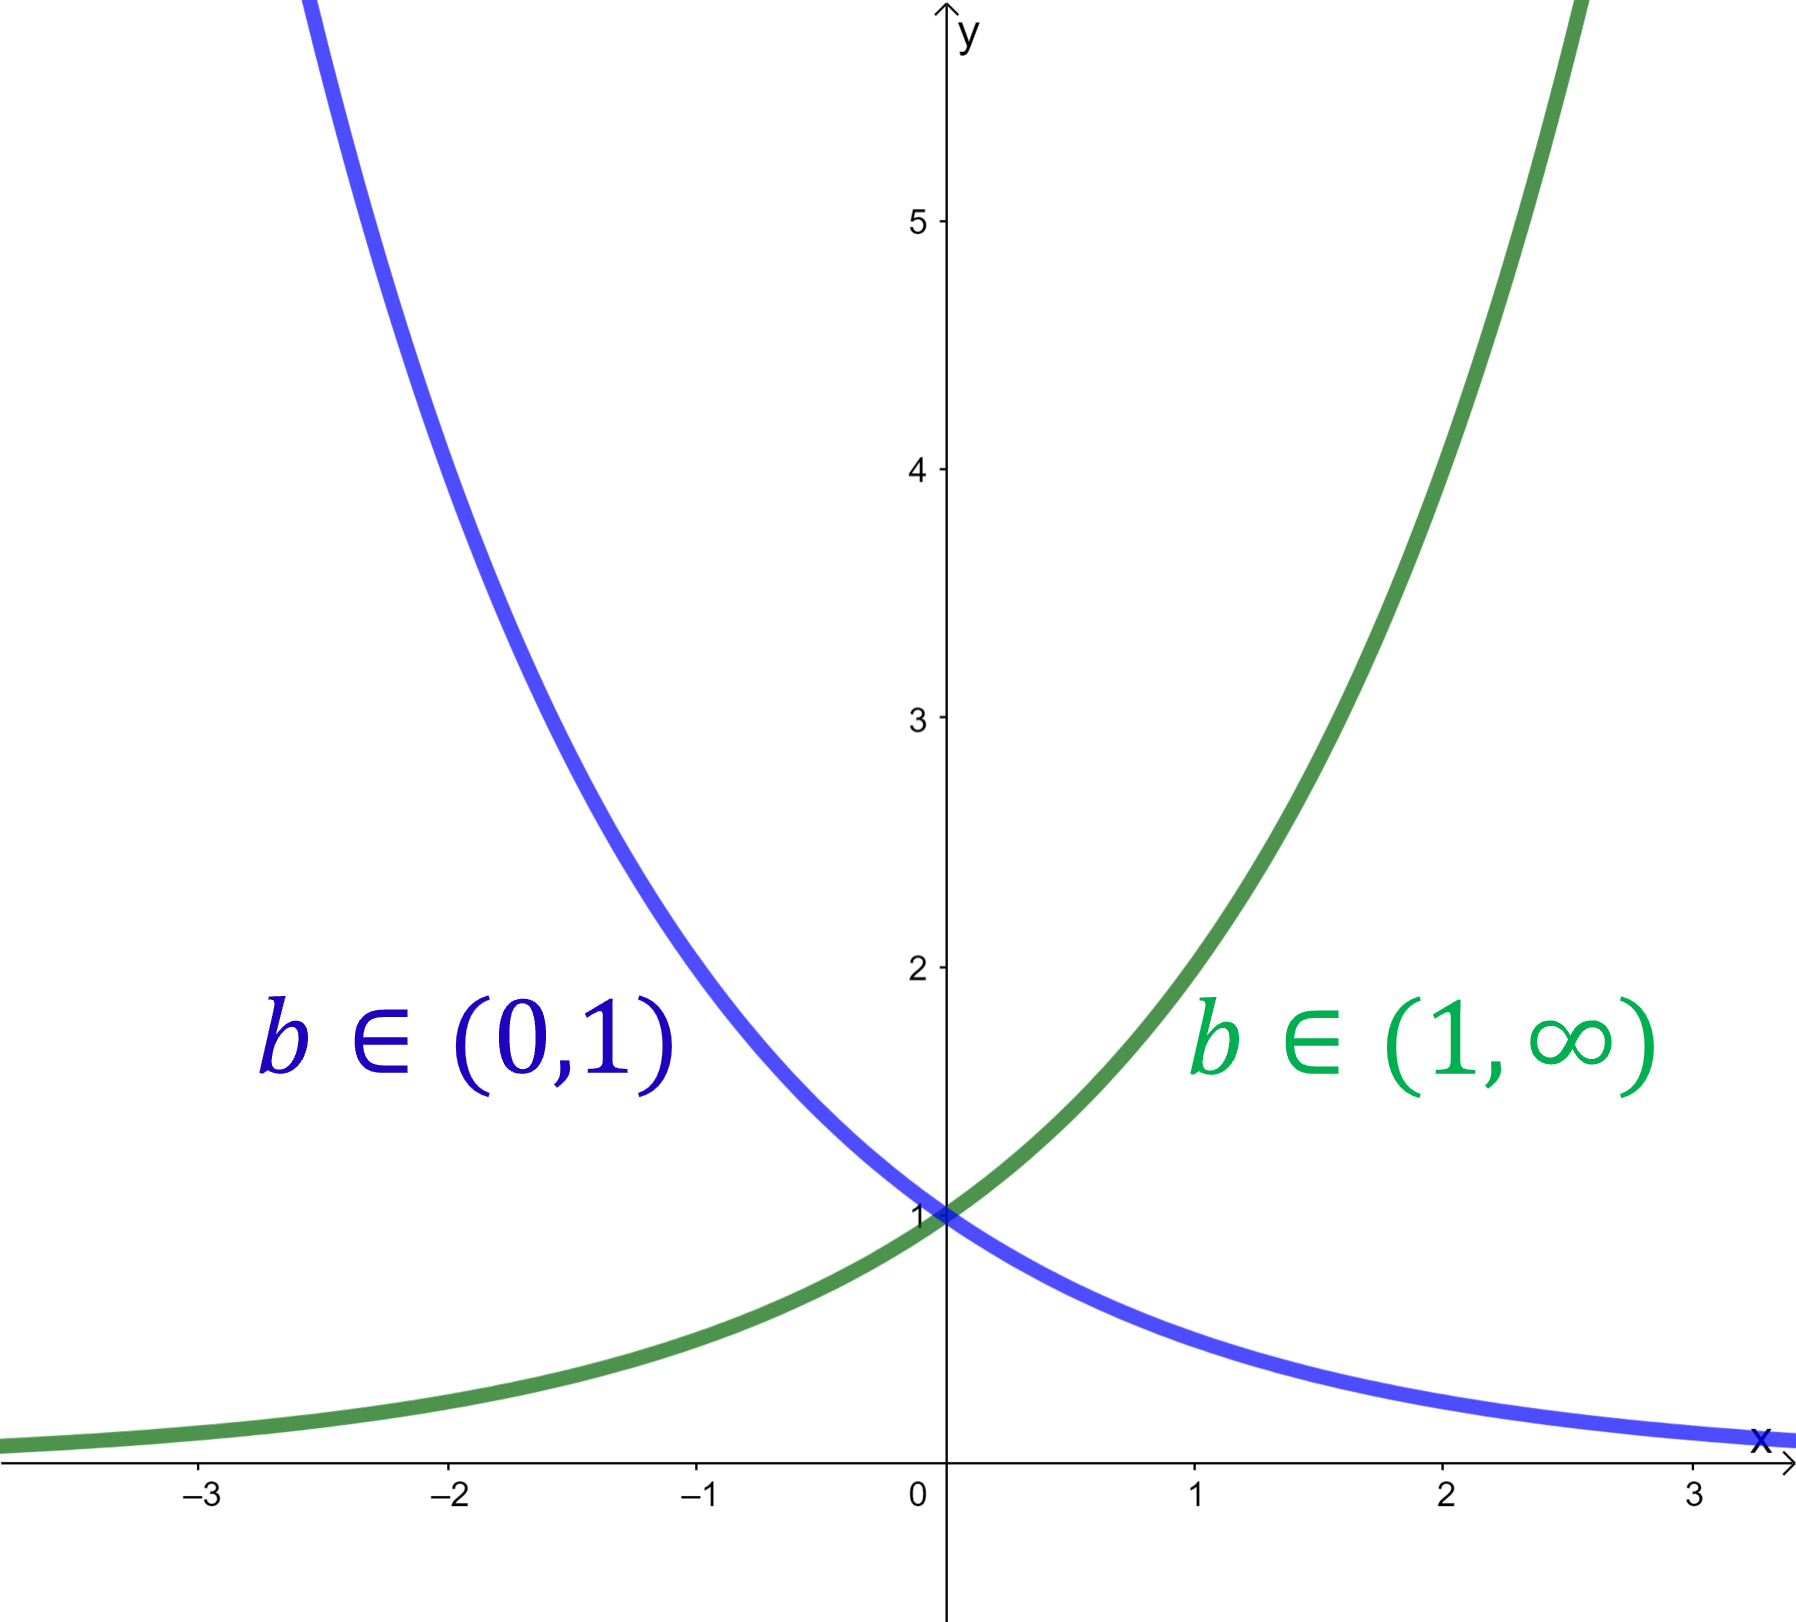
\includegraphics[width=\textwidth]{../Mathematik_1/Bilder/exponentialfunktionen_wachstum_zerfall.png}
\end{minipage}
	\begin{minipage}{0.6\textwidth}
		\begin{itemize}
			\item Definitionsbereich \(D = \mathbb R\). 
			\item Bildmenge $W = (0,\infty)$. 
			\item \(y\)-Achsenabschnitt an der Stelle $y = 1$. 
			\item \textcolor{darkgreen}{streng monoton steigend f�r \(b>1\)}.
			\item \textcolor{blue}{streng monoton fallend f�r \(0<b<1\)}.
		\end{itemize}
\end{minipage}
  
\end{theorembox}

Im vorigen Bild sieht man die Graphen der Funktionen 
\begin{eqnarray*}
	f: x &\mapsto &\textcolor{darkgreen}{2}^{\displaystyle x}\,,\\[2ex]
g: x&\mapsto &\left(\textcolor{blue}{\dfrac12}\right)^{\displaystyle x}\,.
\end{eqnarray*}
Die Graphen der Funktionen spiegeln sich an der \(y\)-Achse und das ist nicht �berraschend, denn 
$$ g(x) = \left(\frac1b\right)^x= b^{-x} = f(-x)\,.$$
F�r das Umformen von Gleichungen mit Exponentialfunktionen sind insbesondere die bereits bekannten Potenzregeln von Bedeutung.\marginpar{Aufgaben} 

\begin{theorembox}{Rechenregeln Exponentialfunktionen}{ }
	Es sei $b\in (0,1)\cup (1,\infty)$ und $x, y \in\mathbb R$. Betrachte die Funktion $x\mapsto b^x\,.$ Es gilt:
\begin{eqnarray*}
		b^0 &=& 1 \\
		b^{x+y} &=& b^x \cdot b^y\\
		b^{-x} &=& \displaystyle{\frac{1}{b^x}}\\ 
		\left( b^x \right)^y &=& b^{x\cdot y}
	\end{eqnarray*}
\end{theorembox}

\subsection{Die Exponentialfunktion $\exp: x\to e^x$}

Unter allen Exponentialfunktionen gibt es eine von besonderer Wichtigkeit. Es ist "\,die Exponentialfunktion"\, mit der Basis \(e\). \(e\) ist eine \textbf{irrationale Zahl} und das hei�t, dass wir Sie nie exakt als Dezimalzahl angeben k�nnen. Aber wir k�nnen sie approxmieren und hierf�r dient das folgende Experiment. Berechnen wir den Ausdruck
\begin{eqnarray*}
	(*) \quad a_n:= \left( 1+\frac1n\right)^n\,, 
\end{eqnarray*}
f�r ein paar $n \in \mathbb N$ aus, beispielsweise f�r $ n = 1,10,100,1000, 10000,100000 $: 

\begin{center}
	\begin{tabular}{c || c|c|c|c|c|c}
		$n$   & $1$ & $10$    & $100$   & $1000$  & $10000$ & $100000$ \\ \hline
	        $a_n$ & $2$ & $2,594$ & $2,705$ & $2,717$ & $2,718$ & $2,718$  
	\end{tabular}
\end{center}

Die Werte legen nahe, dass sich die Zahlen
\[
a_n=\left(1+\frac1n\right)^n
\]
f�r immer gr��ere \(n\) einer festen Zahl ann�hern. Diese Zahl hei�t \textbf{Eulersche Zahl} (\emph{Euler's number}) und wird mit \(e\) bezeichnet.

Mit dem sp�ter eingef�hrten Begriff des Grenzwerts l�sst sich dies schreiben als
\[
e
=
\lim_{n\to\infty}
\left(1+\frac1n\right)^n.
\]
Numerisch gilt
\[
e\approx2{,}718281828459\ldots
\]

Das Verhalten, das wir hier beobachtet haben, werden wir in Abschnitt \abschnittsverweis{MA1-lineare-gleichungssysteme} unter dem Begriff Folgenkonvergenz definieren.  Interessanterweise erhalten wir eine Darstellung f�r jedes Folgenglied \(a_n\) in \( (*)\) mit Hilfe des \underline{Binomischen Satzes}\randverweis{MA1-zahlenmengen}:
\[  
	\left( 1 + \displaystyle{\frac1n} \right)^n = \displaystyle{ \sum\limits_{k=0}^n} \binom{n}{k} \cdot \left( \displaystyle{\frac1n}\right)^k \cdot \left( 1\right)^{n-k} \,.
\]
Dies liefert eine alternative Approximation f�r die Eulersche Zahl, zum Beispiel f�r \(n=1000\):
  \begin{eqnarray*}
	  e = e^{\frac{1000}{1000}} &=& \left(e^{\frac{1}{1000}}\right)^{1000}  = \left(1,0010005\cdots\right)^{1000} \\ & \approx & \left( 1 + \frac{1}{1000}\right)^{1000} = \sum\limits_{k=0}^{1000} \binom{1000}{k} \cdot \frac{1}{1000^k} \\
		  & \approx & 1 + 1 + \frac{1}{2!}\frac{999}{1000}  + \frac{1}{3!}\frac{999\cdot 998}{1000\cdot 1000} + \frac{1}{4!}\frac{999\cdot 998\cdot 997}{1000\cdot 1000 \cdot 1000} + \cdots\\
		  & \approx & 1 + 1 + \frac{1}{2!}  + \frac{1}{3!} + \frac{1}{4!} + \cdots\,.
  \end{eqnarray*}

%Zwischen $2$ und $3$ wird also eine Zahl $e$ liegen, so dass $x\mapsto e^x$ an $x=0 $ genau in einem Winkel von $45^\circ$ steigt. Diese Zahl $e$ hei�t Eulersche Zahl [Euler�s number]. Die Funktion $x \mapsto e^x$ hei�t . 
%
%Aus der Eigenschaft $e\in(2,3)$ l��t sich eine n�herungsweise Berechnung von $e$ herleiten 
%  \begin{eqnarray*}
%    e = e^1 = e^{\frac{1}{1000}\cdot 1000} = \left( e^{\frac{1}{1000}}\right)^{1000}\; \Rightarrow \; e \approx \left( 1 +  \frac{1}{1000} \right)^{1000}\,.
%  \end{eqnarray*}

Dasselbe Prinzip legt f�r die Exponentialfunktion die Approximation
\[
e^x
\approx
\left(1+\frac{x}{n}\right)^n
\]
f�r gro�e \(n\) nahe. Mit dem \underline{binomischen Satz}\randverweis{MA1-zahlenmengen} ergibt sich
\[
\left(1+\frac{x}{n}\right)^n
=
\sum\limits_{k=0}^n
\binom nk\frac{x^k}{n^k}.
\]

F�r gro�e \(n\) n�hern sich die ersten Koeffizienten den Werten
\[
1,\quad 1,\quad \frac1{2!},\quad\frac1{3!},\quad\dots
\]
an. Dies deutet auf die sp�ter exakt zu begr�ndende Darstellung
\[
e^x
=
\sum\limits_{k=0}^{\infty}\frac{x^k}{k!}
=
1+x+\frac{x^2}{2!}+\frac{x^3}{3!}+\dots
\]
hin.

%Mit demselben Trick kann man die Exponentialfunktion $\exp: x\mapsto e^x$ f�r jedes \(x\in\mathbb R\) beliebig genau berechnen, ohne jemals krumme Potenzen zu bilden:
%\begin{eqnarray*}
%	e^x & \approx & \left( 1 + \frac{x}{1000}\right)^{1000} =  \sum\limits_{k=0}^{1000} \binom{1000}{k} \cdot \frac{x}{1000^k}\\
%& \approx & 1 + x + \frac{x^2}{2!}\frac{999}{1000}  + \frac{x^3}{3!}\frac{999\cdot 998}{1000\cdot 1000} + \frac{x^4}{4!}\frac{999\cdot 998\cdot 997}{1000\cdot 1000 \cdot 1000} + \cdots\\
%  &\approx&  1 + x + \frac{1}{2!}x^2 + \frac{1}{3!}x^3 + \frac{1}{4!}x^4 \cdots \,.
%\end{eqnarray*}

%Man kann zeigen, dass die obigen Approximationen f�r \(n\to\infty\) tats�chlich die Eulersche Zahl bzw. die Exponentialfunktion darstellen:\footnote{Um das zu beweisen fehlt uns im Moment das Handwerkszeug.}
%	\[ \begin{array}{rcl}
%		e  &=& \displaystyle{ \sum\limits_{k=0}^\infty} \displaystyle{\frac{1}{k!}}\,,\\
%	e^x  &=& \displaystyle{\sum\limits_{k=0}^\infty}\displaystyle{ \frac{x^k}{k!}}\,. \end{array}
%\]

Die Exponentialfunktionen beschreiben Wachstums- oder Zerfallsprozesse. 
\begin{itemize} 
	\item Die Zinsen werden hier einem Kapital \(K\) �ber einen gewissen Zeitraum zugeschlagen und mit verzinst. Dies f�hrt zu exponentiellem Wachstum des Kapitals. Die Zinseszinsformel lautet: $$K(t) = K(0)\cdot \left(1+\displaystyle{\frac{p}{100}}\right)^t\,,$$ wobei \(p\) die Zinszahl und \(K(0)\) das Anfangskapital darstellt. Bei einem Sparbuch mit \(5\%\) Zinsen pro Jahr hat sich Anfangskapital nach ca. \(14\) Jahren verdoppelt: $$ K(14) = K(0)\cdot \left(1+\displaystyle{\frac{5}{100}}\right)^{14} \approx 1,98\cdot K(0)\,.$$
	\item Das Zerfallsgesetz ist die in der Physik �bliche Bezeichnung der Gleichung, die eine exponentielle zeitliche Abnahme von Gr��en beschreibt. In der Kernphysik gibt das Zerfallsgesetz die Anzahl \(N\) der zu einem Zeitpunkt \(t\) noch nicht zerfallenen Atomkerne einer radioaktiven Substanzprobe an. Diese Anzahl betr�gt $$ N(t) = N(0)\cdot e^{-\lambda t}\,, $$ wobei \(N(0)\) die Anzahl der zum Zeitpunkt \(t=0\) vorhandenen Atomkerne und \(\lambda\) die Zerfallsrate des betreffenden Nuklids ist.
%\item In der Thermodynamik betrachtet man h�ufig Verteilungen von Teilchen auf Niveaus verschiedener Energie $E$. Sind quantenmechanische Effekte egal und ist die Zahl der Teilchen fest und ist die Gesamtenergie fest und ist die Unordnung (Entropie) maximal, ist das Energieniveau $E$ proportional zu $e^{-E/kT}$ besetzt. Dazu kommen noch weitere Faktoren, zum Beispiel, um die Zustandsdichten zu ber�cksichtigen. Dabei ist $k$ die Boltzmann-Konstante, 
%	$$ k = 1,380649 \dot 10^{-23} \mathrm{J}/\mathrm{K}\,.$$ 
%	Diese Verteilung schl�gt sich an vielen Stellen nieder. Die Arrhenius-Gleichung modelliert, wie eine Reaktionsgeschwindigkeit \(v_{\mathrm{reac}}\) von der Temperatur abh�ngt:
%	\begin{exabox}{Arrhenius-Gleichung}{ }
%	$ v_{\mathrm{reac}} \approx e^{-\frac{E}{R\dot T}}\,,$
%\end{exabox}
%wobei \( R=N\cdot k\) die universelle Gaskonstante bezeichnet.  
%\item In  der  Halbleiterdiode  wirkt  die  Raumladungszone  am  $pn$-�bergang  wie  die Aktivierungsenergie in einer chemischen Reaktion. Die ben�tigte Energie wird durch eine in Durchlassrichtung angelegte Spannung $U$ vermindert. Das �bliche Modell f�r kleine Str�me durch eine Diode ist damit:
%
%
%Was sind offensichtlichen Grenzen dieses Modells?
\end{itemize}

\subsection{Logarithmusfunktionen}

Da die Exponentialfunktion
\[
f:\mathbb R\to(0,\infty),
\qquad
x\mapsto b^x,
\]
f�r \(b>0\) und \(b\neq1\) streng monoton und damit bijektiv ist, besitzt sie
eine \underline{Umkehrfunktion}\randverweis{MA1-eigenschaften-von-funktionen}.

Diese Umkehrfunktion hei�t \textbf{Logarithmusfunktion}
(\emph{logarithmic function}) zur Basis \(b\):
\[
\log_b:(0,\infty)\to\mathbb R.
\]

Dabei gilt
\[
y=b^x
\qquad\Longleftrightarrow\qquad
x=\log_b(y).
\]

\noindent{\textbf{Merke:}} 
\begin{itemize}
        \item Ein Logarithmus beantwortet die Frage: Womit muss man die Basis $b$ potenzieren, damit $y$ herauskommt? 
        \item Eine Exponentialfunktion bildet nur auf positive Zahlen ab, also k�nnen Logarithmusfunktionen nur positive Zahlen verarbeiten. 
\end{itemize}

Einige Logarithmusfunktionen sind besonders wichtig und haben deshalb spezielle Bezeichnungen:
\begin{defbox}{Bezeichnungen wichtiger Logarithmusfunktionen}{ }
  \begin{enumerate}
    \item Den Logarithmus zur Basis $e$ schreibt man $\ln:= \log_e$ und nennt ihn den nat�rlichen Logarithmus,
    \item Den Logarithmus zur Basis $10$ schreibt man $\mathrm{lg}:= \log_{10}$,
    \item Den Logarithmus zur Basis $2$ schreibt man $\mathrm{lb}:= \log_2$.
  \end{enumerate}
\end{defbox}

\noindent{\textbf{Vorsicht:}} In Programmiersprachen und in der fortgeschrittenen Mathematik hei�t der nat�rliche Logarithmus oft $\log$. 

Exponentialfunktionen wachsen f�r Basen \(b>1\) sehr schnell, w�hrend Logarithmusfunktionen nur sehr langsam wachsen. Anschaulich gesprochen: Exponentialfunktionen �explodieren�, Logarithmusfunktionen �kriechen�.  Trotz dieses langsamen Wachstums ist die Logarithmusfunktion nach oben unbeschr�nkt.
\begin{exabox}{Monotonie des Logarithmus - es kriecht}{ }
	\begin{minipage}{0.7\textwidth}
	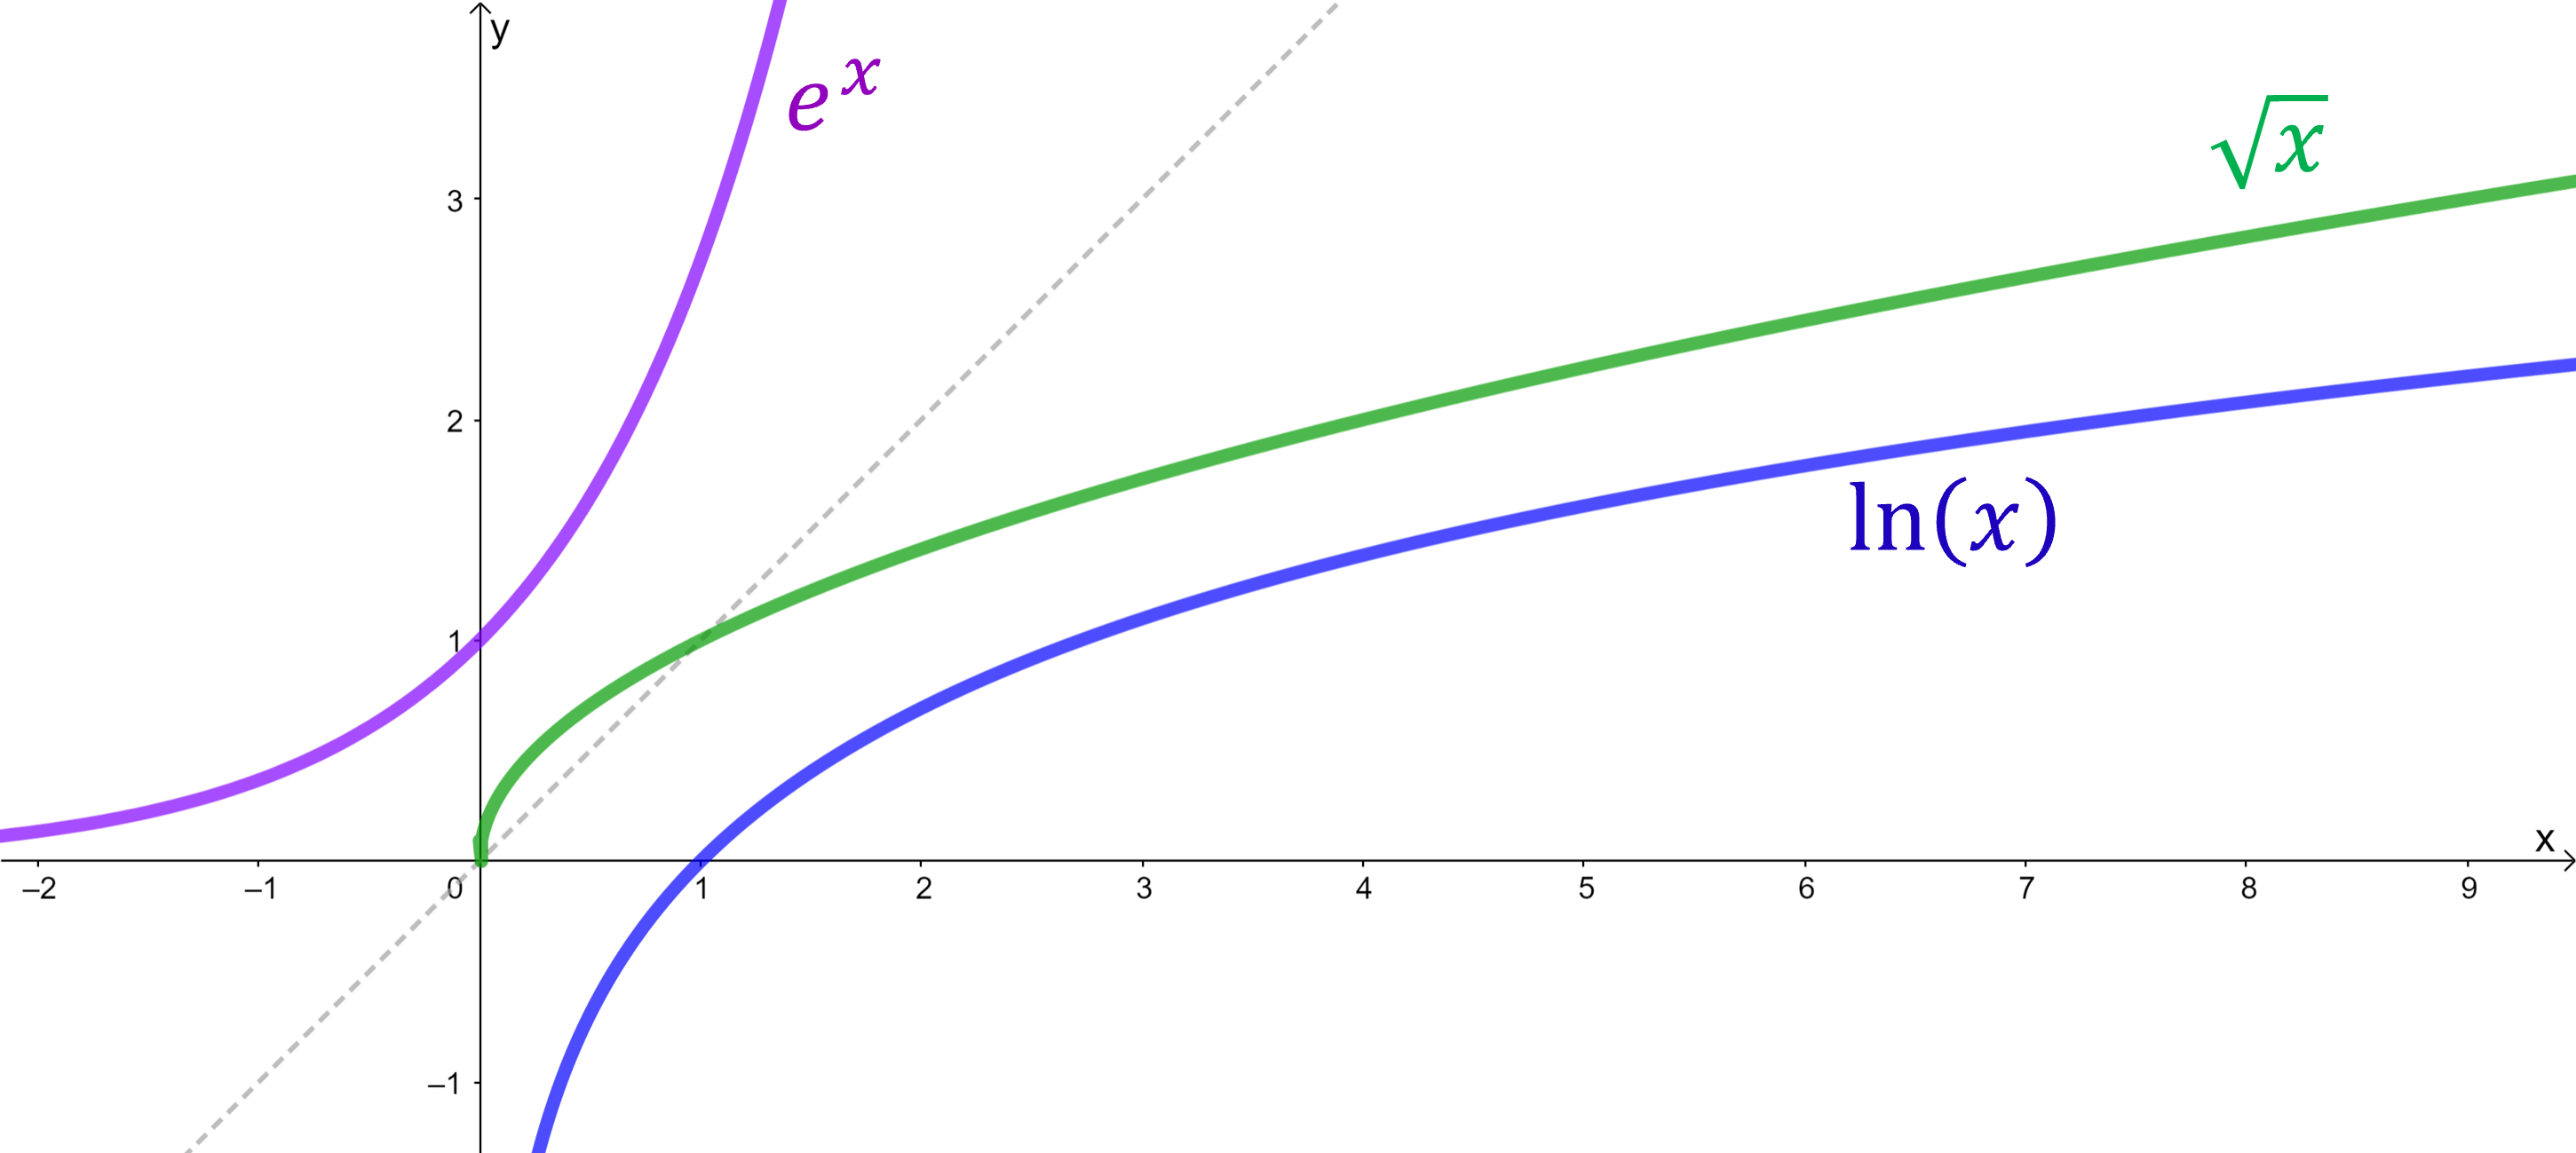
\includegraphics[width=\textwidth]{../Mathematik_1/Bilder/logarithmus_wachstumsvergleich_exponentialfunktion_quadratwurzel.png}
\end{minipage}
	\begin{minipage}{0.3\textwidth}
		\begin{itemize} 
			\item \textcolor{violett}{Exponentialfunktion} 
			\item \textcolor{darkgreen}{Quadratwurzel}
			\item \textcolor{blue}{Logarithmusfunktion}
		\end{itemize}
\end{minipage}
\end{exabox}

Weil die Logarithmusfunktionen die jeweiligen Exponentialfunktionen umkehren, kann  man  aus  den  Potenzrechengesetzen  die  Rechenregeln  f�r  Logarithmusfunktionen folgern:\marginpar{Aufgaben}
\begin{theorembox}{Rechenregeln Logarithmusfunktionen}{ }
	F�r alle $x,y > 0$, $b>0$, $b\not=1$, $z\in \mathbb R$ gilt:
  \begin{eqnarray*}
    \log_b(x\cdot y) &=& \log_b(x) + \log_b(y)\\ 
    \log_b\left(\displaystyle{\frac{x}{y}}\right) &=& \log_b(x) - \log_b(y)\\ 
    \log_b\left(x^z\right) &=&  z\log_b(x)\\ 
    \log_b\left(\sqrt[n]{x}\right) &=&  \displaystyle{\frac1n} \log_b(x), \quad n\in \mathbb N^+\,.
  \end{eqnarray*}
\end{theorembox}

Oft sind am Rechner nur $\mathrm{lg}$ und $\ln$ verf�gbar, keine Logarithmusfunktion zubeliebigen Basen $b$. Dann kann man sich so behelfen: $x=\log_3(7)$, also $7=3^x$, also:
\begin{exabox}{$x=\log_3(7)$}{ }
  $
  \left. \begin{array}{rcl} 7 &=& 10^{\mathrm{lg}(7)}\\
3^x &=& \left( 10^{\mathrm{lg}(3)}\right)^x
\end{array} \right\} \quad \Rightarrow \; \mathrm{lg}(7) = x\cdot \mathrm{lg}(3)  \; \Rightarrow \;  x = \displaystyle{\frac{\mathrm{lg}(7)}{\mathrm{lg}(3)}}\,.
$
\end{exabox}

\begin{theorembox}{Basiswechsel}{ }
	Es gilt 
	\[ \log_b(x) = \dfrac{\log_a(x)}{\log_a(b)} \] 
	f�r alle \(a>0\), \(a\not =1\) und damit insbesondere f�r \(a=e\)
	\[ \log_b(x) = \dfrac{\ln(x)}{\ln(b)} \] 

\end{theorembox}

Auch die Logarithmusfunktionen kommen auf nat�rliche Weise vor:

\begin{itemize}
	\item Schallpegel werden aufgrund der sehr gro�en auftretenden Wertebereiche logarithmisch angegeben. Der Schalldruckpegel ist beispielsweise durch 
		\[ 
			L_p = 20\lg\left(\frac{p}{p_0}\right)\,\mathrm{dB}, \qquad p_0=20\,\mu\mathrm{Pa},
\]
definiert.
\item Au�erdem verh�lt sich der Informationsgehalt logarithmisch:
  $$ \mathrm{lb}\left( \textnormal{Anzahl der Zust\"ande} \right) \; \mathrm{Bits}\,.$$
Zum Beispiel kann man die Zahlen von $0$ bis $255$ in $8$ Bits (Ja-Nein Informationen) speichern.  
\end{itemize}

\begin{exabox}{Gleichungen mit Exponential- und Logarithmusfunktionen}{ }

\textbf{1. Exponentialgleichung}

Gegeben sei die Gleichung
\[
3^{2\cdot x-1}=7.
\]
Die Unbekannte \(x\) steht im Exponenten. Da sich beide Seiten nicht als
Potenzen derselben Basis darstellen lassen, wird die Gleichung logarithmiert:
\[
	\begin{array}{c rcl l}
	& 3^{2\cdot x-1}&=& 7 &\quad\quad \big\|\,\ln(\cdot )\\
\Leftrightarrow\quad  & \ln\left(3^{2\cdot x-1}\right)&=&\ln(7) &\quad\quad \big\|\,\text{Logarithmengesetz anwenden}\\
\Leftrightarrow\quad  & (2\cdot x-1)\ln(3)&=&\ln(7) &\quad\quad \big\|\,\text{vereinfachen}\\
\Leftrightarrow\quad  & 2\cdot x-1&=&\frac{\ln(7)}{\ln(3)} &\quad\quad \big\|\,+1\\
\Leftrightarrow\quad  & 2x&=&1+\frac{\ln(7)}{\ln(3)} &\quad\quad \big\|\, :2\\
\Leftrightarrow\quad  & x&=&\frac12\left(1+\frac{\ln(7)}{\ln(3)}\right). &
\end{array}
\]
Damit lautet die L�sungsmenge \( \mathbb L = \left\{ \frac12\left(1+\frac{\ln(7)}{\ln(3)}\right) \right\}\).

\noindent{\textbf{Fazit:}} Das Logarithmieren erm�glicht hier, den Exponenten mithilfe der Regel \( \ln(a^z)=z\ln(a) \) aus der Potenz herauszul�sen. Die Exponentialgleichung wird dadurch auf eine lineare Gleichung zur�ckgef�hrt.

\bigskip
\textbf{2. Logarithmusgleichung}

Gegeben sei die Gleichung
\[
\ln(x-1)+\ln(x+1)=\ln(8)
\]
Bevor die Gleichung umgeformt wird, muss ihr Definitionsbereich bestimmt
werden. Die Argumente der Logarithmen m�ssen positiv sein: 
\[
x-1>0
\qquad\text{und}\qquad
x+1>0.
\]
Beide Bedingungen sind genau dann erf�llt, wenn \(x>1\).
Damit gilt \( D=(1,\infty) \).  
Innerhalb dieses Definitionsbereichs k�nnen die Logarithmusregeln angewendet
werden:
\[
	\begin{array}{c rcl l}
	& \ln(x-1)+\ln(x+1) &=& \ln(8) &\quad \| \,\text{Logarithmengesetz anwenden}\\
	\Leftrightarrow \quad & \ln\bigl((x-1)(x+1)\bigr) &=& \ln(8) &\quad \| \exp(\cdot ) \\
	\Leftrightarrow \quad & (x-1)(x+1) &=8 &\quad \| \, \text{Eigenschaft Umkehrfunktion} \\ 
	\Leftrightarrow \quad & x^2 &=& 9 &\quad \| \sqrt{\cdot } \\
\Leftrightarrow \quad & |x| &=3.&
\end{array}
\]

Die algebraische Gleichung besitzt damit zun�chst die beiden L�sungen \(x=-3\) und \(x=3\).  F�r die urspr�ngliche Logarithmusgleichung muss jedoch zus�tzlich der Definitionsbereich \( x>1\) ber�cksichtigt werden. Daher entf�llt \(x=-3\), und es bleibt \(\mathbb L=\{3\}\).

\noindent{\textbf{Fazit:}} Eine Logarithmusgleichung kann durch die Logarithmusregeln auf eine algebraische Gleichung zur�ckgef�hrt werden.  Die L�sungen der algebraischen Gleichung sind anschlie�end mit dem Definitionsbereich der urspr�nglichen Gleichung abzugleichen.

\end{exabox}


\subsection{Logarithmische Darstellung}

Exponentialfunktionen und Potenzfunktionen k�nnen sich �ber gro�e Wertebereiche
erstrecken. In einer gew�hnlichen linearen Darstellung sind kleine
Funktionswerte dann h�ufig kaum noch zu erkennen, w�hrend gro�e Funktionswerte
den Graphen dominieren.

Eine logarithmische Skalierung der Achsen erm�glicht nicht nur eine
�bersichtlichere Darstellung solcher Wertebereiche. Sie besitzt au�erdem eine
wichtige mathematische Eigenschaft: Bestimmte nichtlineare Zusammenh�nge
erscheinen bei geeigneter logarithmischer Darstellung als Geraden. Dadurch
k�nnen exponentielle Zusammenh�nge und Potenzgesetze in Messdaten leichter
erkannt und untersucht werden.

\subsubsection*{Exponentielle Zusammenh�nge}

Es sei ein exponentieller Zusammenhang der Form
\[
y=C\cdot b^x,
\qquad
C>0,\quad b>0,\quad b\neq1,
\]
gegeben. Durch Logarithmieren folgt
\[
\begin{aligned}
y&=C\cdot b^x\\
\Longrightarrow\qquad
\ln(y)
&=\ln\left(C\cdot b^x\right)\\
&=\ln(C)+\ln\left(b^x\right)\\
&=\ln(C)+x\ln(b).
\end{aligned}
\]

Damit besteht zwischen \(x\) und \(\ln(y)\) ein linearer Zusammenhang:
\[
\ln(y)=\ln(C)+\ln(b)\cdot x.
\]

Wird also die \(x\)-Achse linear und die \(y\)-Achse logarithmisch skaliert,
erscheint der Graph eines exponentiellen Zusammenhangs als Gerade. Eine solche
Darstellung hei�t \textbf{halblogarithmische Darstellung}
(\emph{semi-logarithmic plot}).

Aus der Geraden lassen sich die Parameter der Exponentialfunktion ablesen:
Der Achsenabschnitt entspricht \(\ln(C)\), die Steigung entspricht
\(\ln(b)\).

\begin{exabox}{Exponentieller Zusammenhang in halblogarithmischer Darstellung}{ }

F�r
\[
y=5\cdot 2^x
\]
ergibt das Logarithmieren
\[
\begin{aligned}
\ln(y)
&=\ln\left(5\cdot2^x\right)\\
&=\ln(5)+x\ln(2).
\end{aligned}
\]
In einer Darstellung von \(\ln(y)\) gegen \(x\) entsteht daher eine Gerade
mit dem Achsenabschnitt
\[
\ln(5)
\]
und der Steigung
\[
\ln(2).
\]

Ein exponentieller Zusammenhang, der in einer gew�hnlichen Darstellung
gekr�mmt erscheint, wird durch das Logarithmieren der \(y\)-Werte also
linearisiert.

\end{exabox}

\subsubsection*{Potenzgesetze}

Ein �hnlicher Zusammenhang entsteht bei Potenzfunktionen. Es sei
\[
y=C\cdot x^\alpha,
\qquad
C>0,\quad x>0.
\]
Durch Logarithmieren folgt
\[
\begin{aligned}
y&=C\cdot x^\alpha\\
\Longrightarrow\qquad
\ln(y)
&=\ln\left(C\cdot x^\alpha\right)\\
&=\ln(C)+\ln\left(x^\alpha\right)\\
&=\ln(C)+\alpha\ln(x).
\end{aligned}
\]

Damit besteht zwischen \(\ln(x)\) und \(\ln(y)\) wiederum ein linearer
Zusammenhang:
\[
\ln(y)=\ln(C)+\alpha\ln(x).
\]

Werden sowohl die \(x\)-Achse als auch die \(y\)-Achse logarithmisch skaliert,
erscheint ein Potenzgesetz als Gerade. Eine solche Darstellung hei�t
\textbf{doppelt logarithmische Darstellung}
(\emph{log-log plot}).

Die Steigung dieser Geraden entspricht unmittelbar dem Exponenten
\(\alpha\). Der Achsenabschnitt entspricht \(\ln(C)\).

\begin{exabox}{Doppelt logarithmische Darstellung}{ }

F�r den Zusammenhang
\[
y=2x^2
\]
gilt
\[
\begin{aligned}
\ln(y)
&=\ln(2x^2)\\
&=\ln(2)+2\ln(x).
\end{aligned}
\]
In einer doppelt logarithmischen Darstellung entsteht daher eine Gerade mit
der Steigung
\[
2.
\]
Der Exponent des Potenzgesetzes kann somit unmittelbar aus der Steigung der
Geraden bestimmt werden.

\medskip
\centering
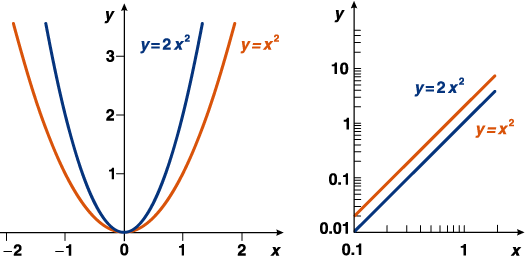
\includegraphics[width=0.6\textwidth]
{../Mathematik_1/Bilder/logarithmische_darstellung_potenzgesetze.png}

\end{exabox}
 % Exponentialfunktion und Logarithmus
\newpage
\setcounter{satz}{0} \setcounter{def}{0} \setcounter{exa}{0}  \section{Trigonometrische Funktionen}\label{MA1-trigonometrische-funktionen}

\begin{table}[H]
  \centering
  \begin{tabularx}{\textwidth}{p{0.9\textwidth} p{0.1\textwidth}}
    \toprule
	  \multicolumn{2}{c}{\textbf{�bersicht �ber Lernziele und Voraussetzungen}}\\
    \midrule
	  \textbf{Lernziele} &\\[.5\normalbaselineskip]
\tabitem Seiten und Winkel in rechtwinkligen Dreiecken mithilfe trigonometrischer Beziehungen bestimmen &\\
\tabitem Winkel zwischen Gradma� und Bogenma� umrechnen &\\
\tabitem Sinus, Kosinus, Tangens und Kotangens am Einheitskreis interpretieren &\\
\tabitem trigonometrische Funktionen beschreiben und skizzieren &\\
\tabitem Arkusfunktionen als Umkehrfunktionen eingeschr�nkter trigonometrischer Funktionen interpretieren &\\
\tabitem trigonometrische Gleichungen unter Ber�cksichtigung von Symmetrie und Periodizit�t l�sen &\\
\tabitem kartesische Koordinaten und Polarkoordinaten ineinander umrechnen &\\[.5\normalbaselineskip]
    \midrule
	  \textbf{Voraussetzungen}& \\[.5\normalbaselineskip]
\tabitem Eigenschaften von Funktionen & \abschnittsverweis{MA1-eigenschaften-von-funktionen}\\
    \bottomrule
  \end{tabularx}
\end{table}

\ifintegriereaufgaben \noindent Die �bungsaufgaben zum Thema finden Sie hier: \hyperref[MA1-trigonometrische-funktionen-aufgaben]{Aufgaben}
\vspace{0.3cm}
\hrule
\fi

\subsection{Rechtwinklige Dreiecke}

Zur Einf�hrung der trigonometrischen Beziehungen werden zun�chst \textbf{rechtwinklige Dreiecke} (\emph{right triangles}) betrachtet.
Per Konvention werden die Seiten, Eckpunkte und Winkel eines rechtwinkligen Dreiecks wie folgt bezeichnet:
\begin{exabox}{�bliche Bezeichnungen im Rechtwinkligen Dreieck}{ }
	\begin{minipage}{0.4\textwidth}
	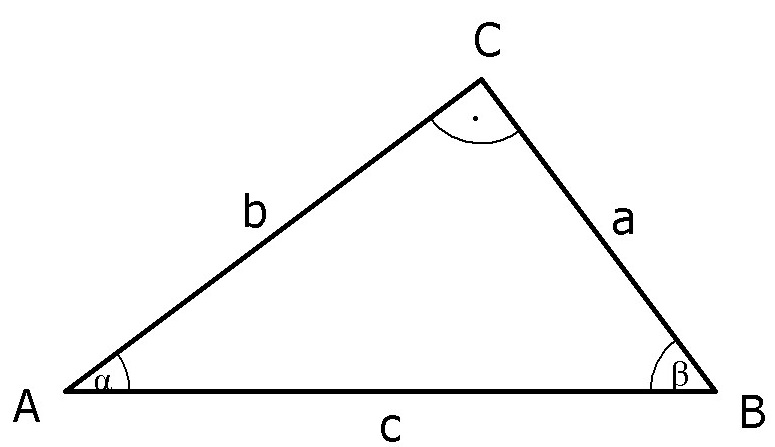
\includegraphics[width=\textwidth]{../Mathematik_1/Bilder/trigonometrie_rechtwinkliges_dreieck_bezeichnungen.png}
\end{minipage}
	\begin{minipage}{0.6\textwidth}

		Die Hypotenuse $c$ ist die Seite im Dreieck, die  dem rechten Winkel gegen�ber liegt. 
Die Bezeichnungen Gegenkathete und Ankathete beziehen sich jeweils auf einen der anderen Winkel. Bezogen auf den Winkel \(\alpha\) ist \(a\) die
Gegenkathete und \(b\) die Ankathete.
\end{minipage}
\end{exabox}

Der \textbf{Satz des Pythagoras} setzt die Seitenl�ngen im rechtwinkligen Dreieck in Beziehung zueinander. Er lautet:
\begin{theorembox}{Satz des Pythagoras}{ }
  Das Quadrat der Hypotenuse ist die Summe aus den Quadraten der Katheten, also $$c^2 = a^2 + b^2\,.$$
\end{theorembox}

Rechtwinklige Dreiecke mit demselben Winkel \(\alpha\) sind �hnlich.  Ihre absoluten Seitenl�ngen k�nnen daher unterschiedlich sein, die Verh�ltnisse entsprechender Seiten sind jedoch gleich.

Diese vom betrachteten Winkel abh�ngigen Seitenverh�ltnisse werden durch \textbf{Sinus} (\emph{sine}) und \textbf{Kosinus} (\emph{cosine}) beschrieben:

\begin{theorembox}{Geometrische Bedeutung von $\sin$ und $\cos$}{ }
  \begin{eqnarray*}
	  \sin(\alpha) &=& \frac{\textnormal{Gegenkathete}}{\textnormal{Hypthenuse}} = \frac{a}{c}\,,\\
    \cos(\alpha) &=& \frac{\textnormal{Ankathete}}{\textnormal{Hypotenuse}} = \frac{b}{c}\,.
  \end{eqnarray*}
\end{theorembox}

Wegen des Satzes des Pythagoras gilt:
\begin{theorembox}{Trigonometrischer Pythagoras - Kreisgleichung}{ }
	\[  (\sin(\alpha))^2 + (\cos(\alpha))^2 = \dfrac{a^2}{c^2} + \dfrac{b^2}{c^2} = \dfrac{a^2+b^2}{c^2}  = 1\,.\]
\end{theorembox}

Das Verh�ltnis der Katheten zueinander hei�t \textbf{Tangens} (\emph{tangent}) bzw. \textbf{Kotangens} (\emph{cotangent}). Das kann man auch mit Sinus und Kosinus ausdr�cken:
\begin{theorembox}{geometrische Bedeutung von $\tan$ und $\cot$}{ }
  \begin{eqnarray*}
    \tan(\alpha) &=&  \frac{\textnormal{Gegenkathete}}{\textnormal{Ankathete}} = \frac{a}{b}\,,\\
    \cot(\alpha) &=&  \frac{\textnormal{Ankathete}}{\textnormal{Gegenkathete}}  = \frac{b}{a}\,.
  \end{eqnarray*}
\end{theorembox}

F�r die Winkel $0^\circ$, $30^\circ$, $45^\circ$, $60^\circ$, $90^\circ$ lassen sich Sinus, Kosinus, Tangens und Kotangents gemetrisch bestimmen:
\begin{center}
  \begin{tabular}{c | c | c | c | c}
    $\alpha$ & $\sin(\alpha)$ & $\cos(\alpha)$ & $\tan(\alpha) $ & $\cot(\alpha)$ \\
    \hline
    $0^\circ$ & $0$ & $1$ & $0$ & -- \\ 
    $30^\circ$ & $1/2$ & $\sqrt{3}/2$ & $1/\sqrt{3}$ & $\sqrt{3}$ \\ 
    $45^\circ$ & $1/\sqrt{2}$ & $1/\sqrt{2}$ & $1$ & $1$ \\ 
    $60^\circ$ & $\sqrt{3}/2$ & $1/2$ & $\sqrt{3}$ & $1/\sqrt{3}$ \\ 
    $90^\circ$ & $1$ & $0$ & -- & $0$ 
  \end{tabular}
\end{center}

\subsection{Allgemeine Dreiecke (+)}

Betrachtet man allgemeine, ebene Dreiecke, so lassen gilt der \textbf{Sinussatz}: die H�he in einem allgemeinen, ebenen Dreieck l��t sich auf zwei Arten berechnen:
$$
    h = b \cdot \sin(\alpha) = a \cdot \sin(\beta) \quad \Rightarrow \frac{\sin(\alpha)}{a} =  \frac{\sin(\beta)}{b}\,.
$$

Weil im allgemeinen Dreieck keine der drei Seiten eine Sonderrolle hat, muss insgesamt gelten:
\begin{theorembox}{Sinussatz}{ }
  $
  \displaystyle{\frac{\sin(\alpha)}{a}} =  \displaystyle{\frac{\sin(\beta)}{b}} = \displaystyle{\frac{\sin(\gamma)}{c}} \quad 
  \Leftrightarrow \displaystyle{\frac{a}{\sin(\alpha)}} = \displaystyle{\frac{b}{\sin(\beta)}} = \displaystyle{\frac{c}{\sin(\gamma)}}\,.
  $
\end{theorembox}
Der Sinussatz dient dazu eine unbekannte Gr��e eines allgemeinen Dreiecks zu bestimmen.

Eine Verallgemeinerung des Satzes von Pythagoras auf allgemeine, ebene Dreiecke ist der \textbf{Kosinussatz}. Er beschreibt, wie die Quadrate der Seiten eines allgemeinen Dreiecks zueinander in Beziehung stehen. 
\vspace{0.2cm}

	\begin{minipage}{0.4\textwidth}
	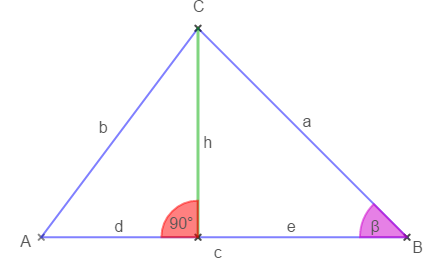
\includegraphics[width=\textwidth]{../Mathematik_1/Bilder/trigonometrie_kosinussatz_hoehenzerlegung.png}
\end{minipage}
	\begin{minipage}{0.6\textwidth}
	$$\begin{array}{rcl} b^2 &=& h^2+d^2 = \left(a\cdot \sin(\beta)\right)^2 + \left( c-a\cdot \cos(\beta)\right)^2 \\
		&=& c^2 - 2\cdot a \cdot c\cos(\beta) + a^2 \underbrace{\left( (\sin(\beta))^2 + (\cos(\beta))^2 \right)}_{\displaystyle{=1}} \\
		&&\Rightarrow b^2 = c^2 - 2\cdot a \cdot c\cos(\beta) + a^2
	\end{array} $$
\end{minipage}
\vspace{0.2cm}

Das muss f�r alle Seiten gleicherma�en gelten. Der Kosinussatz verallgemeinert den Satz des Pythagoras auf allgemeine Dreiecke. In diesen Situationen kann man damit eine unbekannte Gr��e eines allgemeinen Dreiecks bestimmen:
\begin{theorembox}{Kosinussatz}{ }
  \begin{eqnarray*}
    b^2 &=& a^2 + c^2 - 2\cdot a\cdot c \cos\beta\,, \\
    a^2 &=& b^2 + c^2 - 2\cdot b\cdot c \cos\alpha\,, \\
    c^2 &=& a^2 + b^2 - 2\cdot a\cdot b \cos\gamma\,.
  \end{eqnarray*}
\end{theorembox}

\subsection{Was ist das Bogenma�?}

%Dass eine volle Umdrehung als $360^\circ$ bezeichnet wird, ist ein Erbst�ck von den Babyloniern mit ihrem $60$er-Zahlensystem (Einstellung $\mathrm{Deg}$ auf dem Taschenrechner). Man k�nnte zum Beispiel auch $400\mathrm{gon}$ f�r eine Umdrehung nehmen, so dass ein rechter Winkel $100\mathrm{gon}$ oder Neugrad hat (Einstellung $\mathrm{Grad}$ auf dem Taschenrechner). 

Die  nat�rliche  Art,  Winkel  anzugeben,  ist das \textbf{Bogenma�} (\emph{radian}) (Einstellung $\mathrm{Rad}$ auf dem Taschenrechner). Das Bogenma� gibt an, welchen Bogen der Winkel aus dem Einheitskreis abschneidet:\marginpar{\small Aufgaben}
\begin{exabox}{Bogenma�}{ }
	\begin{minipage}{0.4\textwidth}
	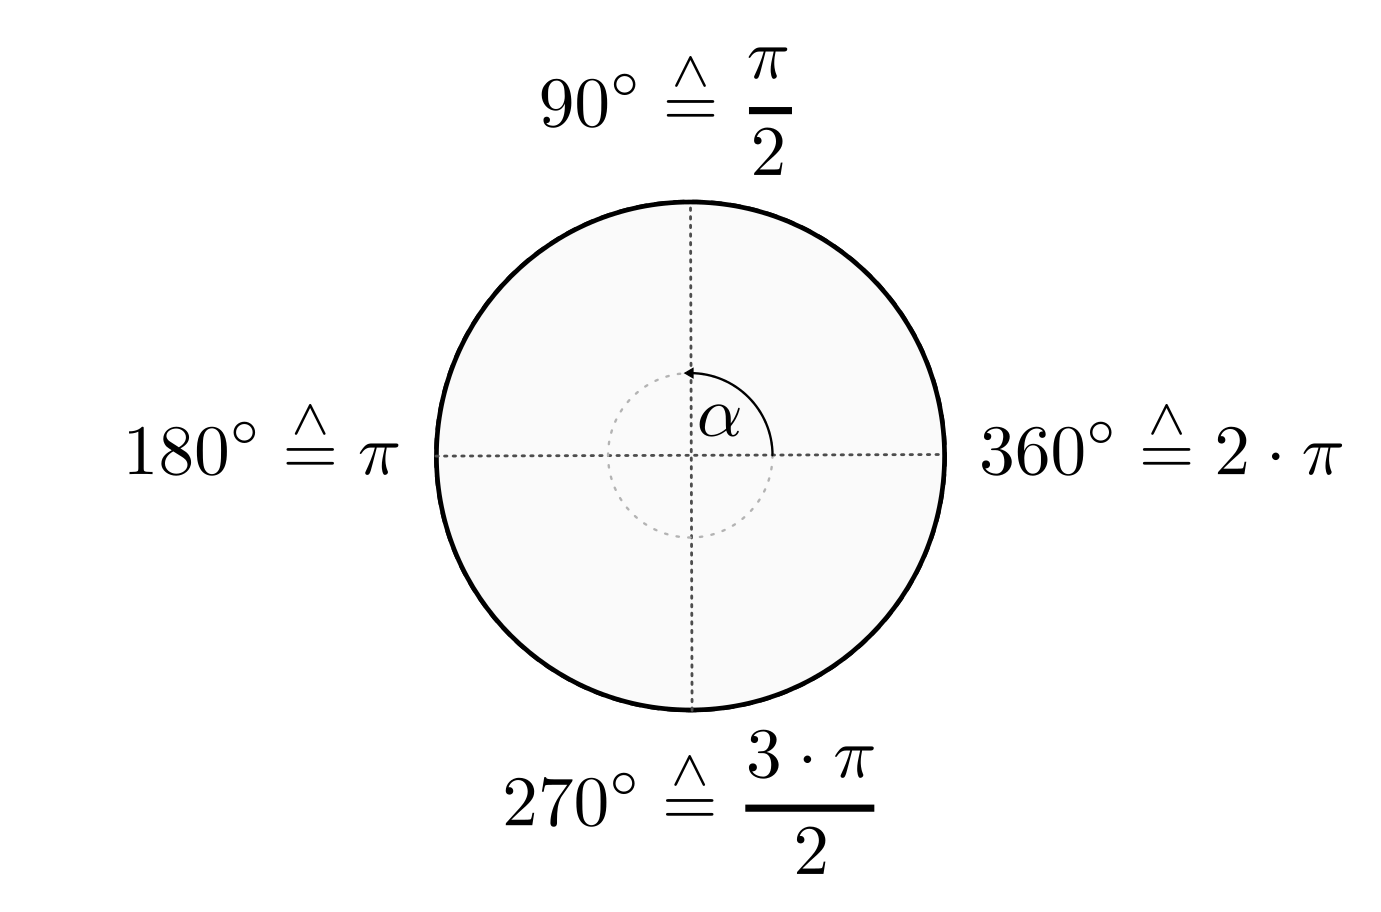
\includegraphics[width=\textwidth]{../Mathematik_1/Bilder/trigonometrie_gradmass_bogenmass.png}
  \end{minipage}
	\begin{minipage}{0.6\textwidth}
    \begin{tabular}{c c c}
    Gradma� & Bogenma� \\
    \hline
    $360^\circ$ & $\widehat = $ & $2\pi $ \\
    $180^\circ$ & $\widehat = $ & $\pi  $ \\
    $90^\circ $ & $\widehat = $ & $\pi/2$ \\
    $60^\circ $ & $\widehat = $ & $\pi/3$ \\
    $45^\circ $ & $\widehat = $ & $\pi/4$
  \end{tabular}
\end{minipage}
\end{exabox}
\noindent\textbf{Bemerkungen:}
\begin{itemize}
	\item Mit Hilfe des Dreisatzes kann man leicht jeden Winkel in Bogenma� umrechnen. Es gilt 
		\[ \varphi_{\mathrm{rad}} = \varphi_{\mathrm{deg}} \cdot \dfrac{\pi}{180^\circ} \] und umgekehrt 
		\[ \varphi_{\mathrm{deg}} = \varphi_{\mathrm{rad}} \cdot \dfrac{180^\circ}{\pi}. \] 

\item Bis auf wenige Ausnahmen %(zum Beispiel einige Teile der 3D-Programmierschnittstelle  OpenGL)  
gibt  man  beim  Programmieren  und  in mathematischer Software Winkel im Bogenma� an. Viele Formeln vereinfachen sich drastisch im Bogenma� und insbesondere gilt $\sin'=\cos$ nur im Bogenma�.
%\begin{center}
%	\includegraphics[width=0.8\textwidth]{../Mathematik_1/Bilder/14_Ableitung_sinus.png}
%\end{center}
\end{itemize}

\subsection{Trigonometrische Funktionen}

Die Definition mithilfe rechtwinkliger Dreiecke beschreibt Sinus und Kosinus zun�chst nur f�r Winkel zwischen \(0\) und \(\pi/2\). Mithilfe des Einheitskreises lassen sich beide Funktionen auf beliebige reelle Winkel erweitern.

Zu einem Winkel \(\varphi\in\mathbb R\) geh�rt auf dem Einheitskreis der Punkt
\[
P(\varphi)
=
\bigl(\cos(\varphi),\sin(\varphi)\bigr).
\]
Der Kosinus ist damit die \(x\)-Koordinate und der Sinus die \(y\)-Koordinate des zugeh�rigen Punktes auf dem Einheitskreis.

\begin{defbox}{Winkelfunktionen f�r \(\varphi \in \mathbb R\)}{ }
	\centering
	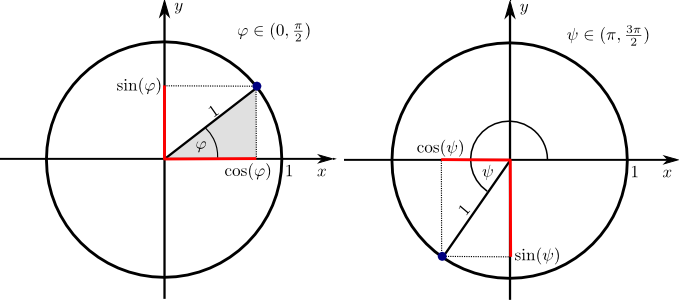
\includegraphics[width=0.6\textwidth]{../Mathematik_1/Bilder/trigonometrie_einheitskreis_sinus_kosinus.png}
\end{defbox}
Und so werden trigonometrische Funktionen zu periodischen Funktionen:
\begin{defbox}{Periodische Funktion}{ }
	\centering
	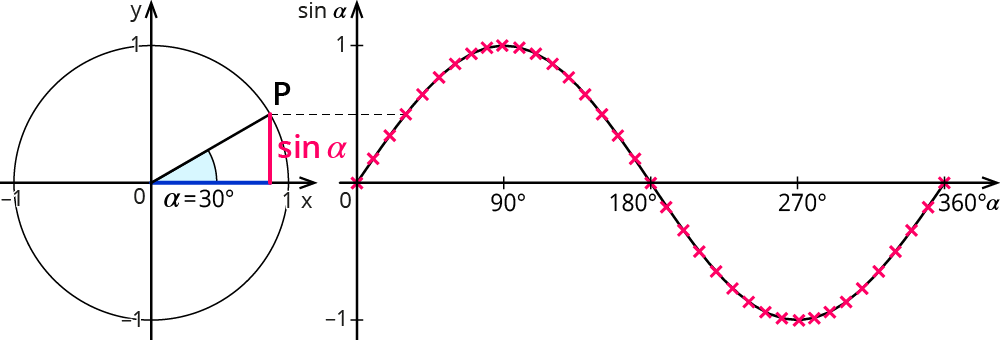
\includegraphics[width=0.6\textwidth]{../Mathematik_1/Bilder/trigonometrie_einheitskreis_sinusverlauf.png}
\end{defbox}

In der folgenden Box sind Eigenschaften der trigonometrischen Funktionen zusammengefasst:

\begin{theorembox}{Eigenschaften trigonometrischer Funktionen}{ }
	F�r alle $k\in \mathbb Z$ gilt:
	\begin{center}
		\begin{tabular}{l | l | l | l | l | l | l}
			 & Definitionsbereich & Bildmenge & Symmetrie & Periode & Nullstellen & Pole \\
			\hline
			$\sin$ & $\mathbb R$ & $[-1,1]$ & ungerade & $2\pi$ & $k\cdot \pi$ & -- \\
			$\cos$ & $\mathbb R$ & $[-1,1]$ & gerade & $2\pi$ & $\pi/2 + k\cdot \pi$ & -- \\
			$\tan$ & $\mathbb R\setminus \{ \pi/2+k\cdot \pi\}$ & $\mathbb R$ & ungerade & $\pi$ & $k\cdot \pi$ & $\pi/2+k\cdot \pi$ \\
			$\mathrm{cot}$ & $\mathbb R\setminus \{ k\cdot \pi\}$ & $\mathbb R$ & ungerade & $\pi$ & $\pi/2+k\cdot \pi$ & $k\cdot \pi$ 
		\end{tabular}
	\end{center}
\end{theorembox}

% Den Sinus und den Kosinus braucht man in den Naturwissenschaften zur Beschreibung von harmonischen Schwingungen und deren �berlagerungen. Eine Schwingung ist eine sich zeitlich wiederholende Ver�nderung einer Zustandsgr��e. 
% \begin{defbox}{Harmonische Schwingung}{ }
% 	Eine harmonische Schwingung wird durch 
% 	$$ s(t) = A\cdot \sin(\omega\cdot t + \varphi_0)\quad \textnormal{bzw.}\quad c(t) = A\cdot \cos(\omega\cdot t+ \varphi_0) $$
% 	beschrieben, wobei
% 	\begin{itemize}
% 		\item \(A\) die Amplitude,
% 		\item $\varphi_0$ die Nullphase und 
% 		\item \(\omega\) die Kreisfrequenz der Schwingung ist.
% 	\end{itemize}
% 	Das zeitabh�ngige Argument einer harmonischen Schwingung, $\varphi(t) = \omega\cdot t + \varphi_0$, bezeichnet man als Phase. 
% 	Die Schwingungsdauer oder Periode $T$ und die Frequenz $f$ betragen $$ T = \frac{2\pi}{\omega}, \quad f= \frac{1}{T} = \frac{\omega}{2\pi}\,. $$
% \end{defbox}

\subsection{Arkusfunktionen}\label{MA1-trigonometrische-funktionen-arkusfunktionen}

Um von Seitenverh�ltnissen oder mit dem Sinus- oder dem Kosinussatz auf Winkel zu schlie�en, muss man die Winkelfunktion umkehren. Allerdings sind trigonometrische Funktionen periodisch, also \underline{nicht umkehrbar}\randverweis{MA1-eigenschaften-von-funktionen}. Die Idee besteht darin, einen sinnvollen Winkel zur�ckzuliefern -- auch wenn das nicht der einzig m�gliche ist. Und genau das machen die Arkusfunktionen\footnote{Arkus $=$ Bogen, also Winkel}.

\begin{defbox}{Arkusfunktionen}{ }
	\begin{eqnarray*}
		\begin{array}{lcl l }
			\arcsin: [-1,1] &\to& [-\pi/2, \pi/2], \; &x\mapsto \arcsin(x) \\[1ex]
			\arccos: [-1,1] &\to& [0, \pi], \; &x\mapsto \arccos(x)  \\[1ex]
			\arctan: (-\infty,\infty) &\to& (- \pi/2, \pi/2), \; &x\mapsto \arctan(x)\\[1ex]
			\mathrm{arccot}: (-\infty,\infty) &\to& (0,\pi), \; &x\mapsto \mathrm{arccot}(x) 
\end{array}
\end{eqnarray*}
\textbf{Bemerkung:} es gilt $\mathrm{arccot}(x) = \frac{\pi}{2} - \arctan(x)$.
\end{defbox}

\noindent \textbf{Bemerkungen:}
\begin{itemize}
	\item �hnlich wie bei geradzahligen \underline{Potenzfunktionen}\randverweis{MA1-potenz-und-wurzelfunktionen} ist die Idee eine trigonometrische Funktion auf ein maximales Intervall einzuschr�nken, auf dem sie injektiv ist. Das Intervall ist zun�chst willk�rlich.
	Der Sinus ist auf dem Intervall
\[
I=[-\pi/2,\pi/2]
\]
streng monoton steigend und damit injektiv. Gleichzeitig nimmt er dort alle
Werte aus \([-1,1]\) an. Die Einschr�nkung
\[
\sin:[-\pi/2,\pi/2]\to[-1,1]
\]
ist daher bijektiv und besitzt eine Umkehrfunktion. Die Umkehrfunktion, die den Sinus auf \(I\) umkehrt, nennt sich \textbf{Arkussinus}.  

	\item Dass die  Arkussinus Funktion  keine  Winkel  �ber  $90^\circ$ liefert, ist  dann  gef�hrlich, wenn man mit dem Sinussatz arbeitet: Bei der Anwendung des Sinussatzes kann aus
\[
\sin(\beta)=s
\]
nicht unmittelbar auf einen eindeutigen Winkel geschlossen werden. F�r
\(0<s<1\) besitzen im Intervall \((0,\pi)\) im Allgemeinen die beiden Winkel
\[
\beta
\qquad\text{und}\qquad
\pi-\beta
\]
denselben Sinuswert. Je nach den �brigen gegebenen Gr��en k�nnen daher zwei verschiedene Dreiecke m�glich sein.	
	\item Der Arkustangens liefert also nur Werte von $-90^\circ \widehat= -\pi/2$ bis $90^\circ \widehat =\pi/2$ und keine gesamte Umdrehung von $-180^\circ=-\pi$ bis $180^\circ =\pi$. Das Problem ist, dass der Tangens nicht unterscheiden kann, ob ein Punkt \( (x|y)\) im ersten oder dritten bzw. im zweiten oder vierten Quadranten liegt, denn die Vorzeicheninformation geht bei der Division verloren:
$$\tan(\varphi) = \frac{y_1}{x_1} =\frac{y_2}{x_2} = \tan(\varphi +\pi), \quad \mathrm{mit} \; y_2=-y_1, \quad x_2=-x_1\,.$$ 
\end{itemize}

Das zuletzt genannte Problem kann behoben werden, wenn man die Vorzeicheninformation der Koordinaten \(x\) und \(y\) wei� und genau das wird in der Praxis auch getan: in fast allen Programmiersprachen gibt es eine Funktion namens $\verb-atan2-$. Diese Funktion liefert Werte aus $(-\pi,\pi]$ zur�ck, also eine komplette Umdrehung. Die getrennte �bergabe der Koordinaten \(x\) und \(y\) erh�lt die Vorzeicheninformation: \footnote{Normalerweise ist die Reihenfolge $y$ dann $x$,  entsprechend $"\dfrac{y}{x}"$, aber man muss aufpassen, denn manchmal ist die Reihenfolge auch "$x,y$".}

\begin{exabox}{\(\mathrm{atan2}\)}{ }
	\begin{minipage}{0.4\textwidth}
	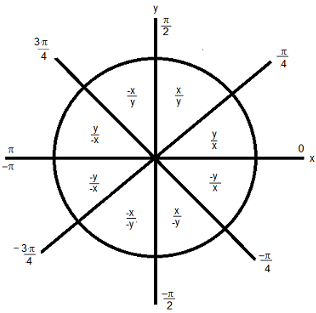
\includegraphics[width=\textwidth]{../Mathematik_1/Bilder/trigonometrie_atan2_quadranten_winkel.png}
\end{minipage}
	\begin{minipage}{0.6\textwidth}
		Der herk�mmliche Arkustangens kann Punkte im ersten und dritten Quadranten nicht unterscheiden: 
		\[ 
			\begin{array}{rcl} 
				(3|3) &\Rightarrow & \begin{cases} \verb-atan2-(3,3) &= \frac14 \pi \,,\\ \arctan(1) &= \frac14 \pi \end{cases}\\[2ex] 
				(-3|-3) &\Rightarrow & \begin{cases} \verb-atan2-(-3,-3) &= -\frac34 \pi \,,\\ \arctan(1) &= \frac14 \pi \end{cases}\\[2ex] 
			\end{array}
		\]
		Der herk�mmliche Arkustangens kann Punkte im zweiten und vierten Quadranten nicht unterscheiden: 
		\[ 
			\begin{array}{rcl} 
				(-3|3) &\Rightarrow & \begin{cases} \verb-atan2-(3,-3) &= \frac34 \pi \,,\\ \arctan(-1) &= -\frac{1}{4} \pi \end{cases}\\[2ex] 
				(3|-3) &\Rightarrow & \begin{cases} \verb-atan2-(-3,3) &= -\frac14 \pi \,,\\ \arctan(-1) &= -\frac14 \pi \end{cases}
			\end{array}
		\]
	\end{minipage}
\end{exabox}

Der Arkustangens kommt dann zum Einsatz, wenn man von kartesischen Koordinaten in Polarkoordinaten umrechnen m�chte. 
\begin{defbox}{Polarkoordinaten mit Hilfe von \(\mathrm{atan2}\) }{ }
	Jeder Punkt $(x,y) \in \mathbb R^2$ kann in der Form 
	$$ 
	x= r\cdot \cos(\varphi), \quad y=r\cdot \sin(\varphi)
	$$ 
	mit $r\in \mathbb R^+_0$ und $\varphi \in (-\pi, \pi]$ dargestellt werden. Es gilt 
	$$
	r=\sqrt{x^2+y^2}, \quad 
\varphi=\operatorname{atan2}(y,x):=
\begin{cases}
\arctan(y/x), & x>0,\\[1ex]
\arctan(y/x)+\pi, & x<0,\;y\geq0,\\[1ex]
\arctan(y/x)-\pi, & x<0,\;y<0,\\[1ex]
\pi/2, & x=0,\;y>0,\\[1ex]
-\pi/2, & x=0,\;y<0.
\end{cases}
	$$
	\noindent{\textbf{Bemerkungen}}
	\begin{itemize}
		\item Die Werte $(r,\varphi)$ hei�en Polarkoordinaten von $(x,y)$.
		\item F�r den Ursprung \( (0,0)\) ist der Winkel \(\varphi \) nicht definiert.
		\item Die Funktion \(\operatorname{atan2}\) besitzt damit die folgende Signatur: \[ \operatorname{atan2}: \mathbb R^2 \setminus \{ (0, 0 )\} \to (-\pi, \pi]\].
	\end{itemize}
\end{defbox}


\begin{exabox}{L�sen einer trigonometrischen Gleichung}{ }

	Gesucht sind \emph{alle} reellen L�sungen der Gleichung
\[
\sin(x)=\frac12.
\]

Aus den bekannten Werten der Sinusfunktion folgt zun�chst
\[
\sin\left(\frac{\pi}{6}\right)=\frac12.
\]
Damit ist
\[
x_1=\frac{\pi}{6}
\]
\emph{eine} L�sung der Gleichung.

Diese L�sung ist jedoch nicht die einzige. Am Einheitskreis entspricht der Sinus der \(y\)-Koordinate eines Punktes. Die \(y\)-Koordinate \(\frac12\) wird innerhalb einer vollst�ndigen Periode an zwei verschiedenen Stellen angenommen. Aufgrund der Symmetrie des Sinus gilt
\[
\sin(x)=\sin(\pi-x).
\]
Aus
\[
x_1=\frac{\pi}{6}
\]
ergibt sich daher als zweite L�sung innerhalb des Intervalls
\([0,2\pi)\)
\[
x_2
=
\pi-\frac{\pi}{6}
=
\frac{5\pi}{6}.
\]

Damit besitzt die Gleichung innerhalb einer vollst�ndigen Periode zwei L�sungen, \( x_1 = \frac{\pi}{6}\) und \(x_2 = \frac{5\pi}{6}\).

Da die Sinusfunktion die Periode \(2\pi\) besitzt, wiederholen sich diese
L�sungen nach jeder vollst�ndigen Umdrehung:
\[
\sin(x+2k\pi)=\sin(x),
\qquad k\in\mathbb Z.
\]
Damit ergeben sich alle reellen L�sungen zu
\[
x=\frac{\pi}{6}+2k\pi
\quad\text{oder}\quad
x=\frac{5\pi}{6}+2k\pi,
\qquad k\in\mathbb Z.
\]

Die L�sungsmenge kann entsprechend geschrieben werden als
\[
\mathbb L
=
\left\{
\frac{\pi}{6}+2k\pi:k\in\mathbb Z
\right\}
\cup
\left\{
\frac{5\pi}{6}+2k\pi:k\in\mathbb Z
\right\}.
\]

Das Beispiel zeigt einen wesentlichen Unterschied zu vielen bisher
betrachteten Gleichungen: Aufgrund der Periodizit�t einer trigonometrischen
Funktion k�nnen aus einer L�sung unendlich viele weitere L�sungen entstehen.
F�r die vollst�ndige L�sungsmenge m�ssen daher sowohl die verschiedenen
L�sungen innerhalb einer Periode als auch die periodischen Wiederholungen
ber�cksichtigt werden.

\end{exabox}
 % Trigonometrische Funktionen
\newpage
\setcounter{satz}{0} \setcounter{def}{0} \setcounter{exa}{0}  \section{Verkettung von Funktionen}\label{MA1-verkettung-von-funktionen}

\begin{table}[H]
  \centering
  \begin{tabularx}{\textwidth}{p{0.9\textwidth} p{0.1\textwidth}}
    \toprule
	  \multicolumn{2}{c}{\textbf{�bersicht �ber Lernziele und Voraussetzungen}}\\
    \midrule
    \textbf{Lernziele} &\\[.5\normalbaselineskip]
\tabitem verkettete Funktionen erkennen und in ihre Teilfunktionen zerlegen &\\
\tabitem die Abbildungsvorschrift einer Verkettung bestimmen &\\
\tabitem Definitionsbereich und Bildmenge einer Verkettung bestimmen &\\
\tabitem Verschiebung, Skalierung und Spiegelung von Funktionsgraphen als Verkettungen darstellen &\\
\tabitem Funktionsgraphen durch Kompositionen systematisch ver�ndern &\\
\tabitem harmonische Schwingungen aus der Sinusfunktion systematisch konstruieren und die Bedeutung ihrer Parameter erkl�ren &\\[.5\normalbaselineskip]
\midrule
\textbf{Voraussetzungen} &\\[.5\normalbaselineskip]
\tabitem Funktionsbegriff, Definitionsbereich und Bildmenge & \abschnittsverweis{MA1-funktionen}\\
\tabitem Eigenschaften von Funktionen & \abschnittsverweis{MA1-eigenschaften-von-funktionen}\\
\tabitem grundlegende Funktionsklassen & \abschnittsverweis{MA1-lineare-funktionen}-\abschnittsverweis{MA1-trigonometrische-funktionen}\\
    \bottomrule
  \end{tabularx}
\end{table}

\ifintegriereaufgaben \noindent �bungsaufgaben zum Thema finden Sie hier: \hyperref[MA1-verkettung-von-funktionen-aufgaben]{Aufgaben}
\vspace{0.3cm}
\hrule
\fi

\subsection{Was ist eine Verkettung?}

Funktionen k�nnen nicht nur miteinander addiert oder multipliziert werden.
Der Funktionswert einer Funktion kann auch als Eingabe einer weiteren
Funktion verwendet werden.

Es seien beispielsweise zwei Funktionen \(g\) und \(f\) gegeben. Zun�chst
wird \(g\) auf \(x\) angewendet:
\[
x\mapsto g(x).
\]
Das Ergebnis \(g(x)\) wird anschlie�end als Eingabe der Funktion \(f\)
verwendet:
\[
g(x)\mapsto f(g(x)).
\]

Diese Hintereinanderausf�hrung hei�t \textbf{Verkettung} oder
\textbf{Komposition} (\emph{composition}) der Funktionen \(f\) und \(g\).
Sie wird mit
\[
f\circ g
\]
bezeichnet und ist selbst wieder eine Funktion:
\[
(f\circ g)(x)=f(g(x)).
\]

Die Schreibweise \(f\circ g\) wird dabei von rechts nach links gelesen:
Zuerst wird \(g\), anschlie�end \(f\) angewendet. Daher wird
\(f\circ g\) auch als �\(f\) nach \(g\)� bezeichnet.

\begin{exabox}{Verkettung als Maschine}{ }
	\centering
	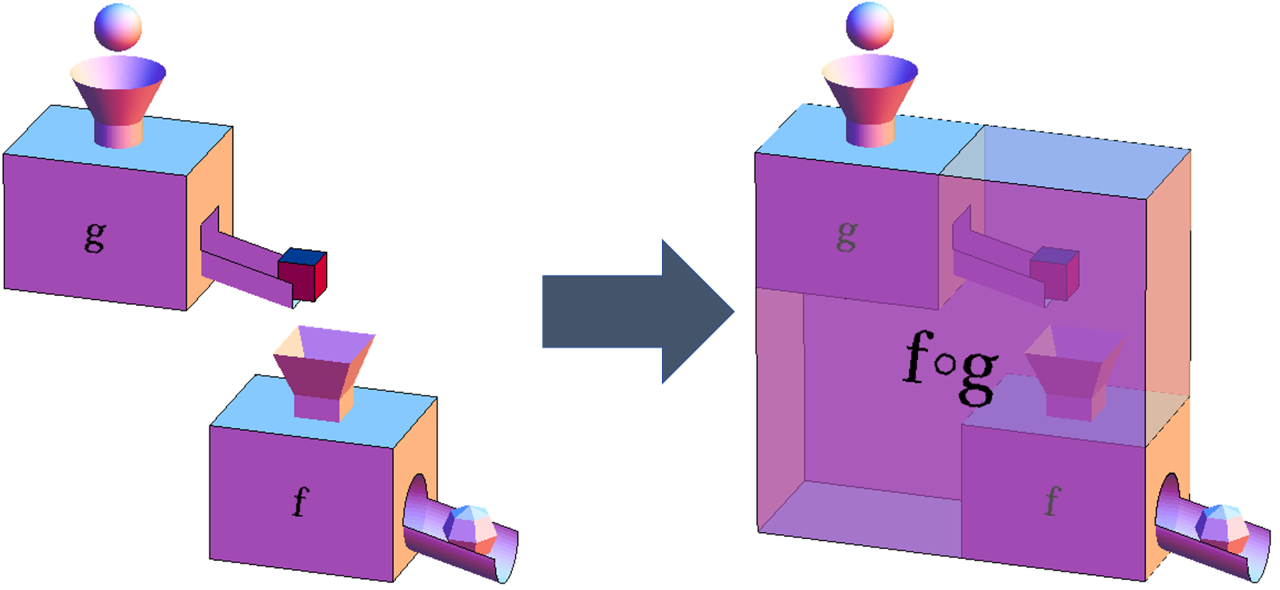
\includegraphics[width=0.7\textwidth]{../Mathematik_1/Bilder/funktionen_verkettung_maschinenmodell.png}
\end{exabox}

Die Reihenfolge ist wichtig: Verkettung ist im Allgemeinen \emph{nicht} kommutativ.

\begin{exabox}{Reihenfolge ist entscheidend}{ }

Es seien
\[
f(x)=\sin(x)
\qquad\text{und}\qquad
g(x)=e^x.
\]
Dann ergibt sich in der einen Reihenfolge
\[
(f\circ g)(x)
=
\sin(e^x),
\qquad
f\circ g:\mathbb R\to[-1,1].
\]

In der umgekehrten Reihenfolge entsteht dagegen
\[
(g\circ f)(x)
=
e^{\sin(x)},
\qquad
g\circ f:\mathbb R\to[e^{-1},e].
\]

Damit gilt im Allgemeinen
\[
f\circ g\neq g\circ f.
\]
Die Verkettung von Funktionen ist also im Allgemeinen nicht kommutativ.

\end{exabox}

Die unterschiedliche Reihenfolge ver�ndert damit nicht nur die Abbildungsvorschrift, sondern auch das Verhalten und die Bildmenge der entstehenden Funktion.

\subsubsection*{Definitionsbereich einer Verkettung}

Bei einer Verkettung muss nicht nur die innere Funktion \(g\) an der Stelle
\(x\) definiert sein. Ihr Funktionswert \(g(x)\) muss au�erdem eine zul�ssige
Eingabe f�r die �u�ere Funktion \(f\) sein.

F�r die Verkettung
\[
(f\circ g)(x)=f(g(x))
\]
gilt daher
\[
D_{f\circ g}
=
\{x\in D_g:g(x)\in D_f\}.
\]

\begin{exabox}{Definitionsbereich einer Verkettung bestimmen}{ }

Betrachtet wird die Verkettung
\[
x\mapsto\sqrt{\ln(x)}.
\]
Die innere Funktion
\[
g(x)=\ln(x)
\]
ist zun�chst nur f�r
\[
x>0
\]
definiert.

Die �u�ere Funktion
\[
f(y)=\sqrt y
\]
kann au�erdem nur nichtnegative Werte verarbeiten. Daher muss zus�tzlich
\[
\ln(x)\geq0
\]
gelten. Dies ist genau f�r
\[
x\geq1
\]
der Fall.

Damit besitzt die Verkettung den Definitionsbereich
\[
D_{f\circ g}=[1,\infty)
\]
und es gilt
\[
\sqrt{\;\cdot\;}\circ\ln:
[1,\infty)\to[0,\infty),
\qquad
x\mapsto\sqrt{\ln(x)}.
\]

\end{exabox}

\begin{exabox}{Eine verkettete Funktion in Teilfunktionen zerlegen}{ }

Betrachtet wird die Funktion
\[
x\mapsto\frac{1}{(\sin x)^2+1}.
\]

Die Abbildungsvorschrift l�sst sich als Folge von drei Schritten lesen:
\[
x
\longmapsto
\sin(x)
\longmapsto
(\sin x)^2+1
\longmapsto
\frac{1}{(\sin x)^2+1}.
\]

Dazu k�nnen die drei Funktionen
\[
h(x)=\sin(x),
\qquad
g(x)=x^2+1,
\qquad
f(x)=\frac1x
\]
definiert werden. Damit gilt
\[
(f\circ g\circ h)(x)
=
f(g(h(x)))
=
\frac{1}{(\sin x)^2+1}.
\]

Die �u�erste Rechenoperation geh�rt dabei zur �u�ersten Funktion \(f\), die
innerste Rechenoperation zur zuerst ausgef�hrten Funktion \(h\).

\end{exabox}

\noindent\textbf{Bemerkung:}
\begin{itemize}
	\item Das Erkennen solcher Verkettungen wird sp�ter bei der Differentialrechnung erneut wichtig. Die Kettenregel beschreibt, wie die Ableitung einer verketteten Funktion aus den Ableitungen ihrer Teilfunktionen bestimmt werden
kann.
\item Wird eine Funktion mehrfach mit sich selbst verkettet, spricht man von einer \textbf{Iteration}. 
F�r die dreifache Iteration findet sich daher auch die Schreibweise
\[
f^3:=f\circ f\circ f.
\]
Diese Notation ist allerdings kontextabh�ngig und darf nicht mit der dritten Potenz des Funktionswertes, also der Zahl \( (f(x))^3 \) verwechselt werden.	
\item Die Schreibweise \(f^{-1}\) bezeichnet die Umkehrfunktion von \(f\), sofern diese existiert.
\end{itemize}

\subsection{Systematische Ver�nderung von Funktionsgraphen}

Viele typische Ver�nderungen von Funktionsgraphen lassen sich als
Verkettungen mit linearen Funktionen verstehen. Dabei ist entscheidend, an
welcher Stelle der Verkettung die lineare Funktion steht.

Wird eine Funktion
\[
g(y)=my+b
\]
\textbf{nach} \(f\) angewendet, so gilt
\[
(g\circ f)(x)=m\,f(x)+b.
\]
Die Ver�nderung betrifft unmittelbar die Funktionswerte und wirkt daher in
\textbf{vertikaler Richtung}.

Wird dagegen eine lineare Funktion
\[
g(x)=k(x+a)
\]
\textbf{vor} \(f\) angewendet, so gilt
\[
(f\circ g)(x)=f\!\bigl(k(x+a)\bigr).
\]
In diesem Fall wird das Argument von \(f\) ver�ndert. Die Ver�nderung wirkt
daher in \textbf{horizontaler Richtung}.

Im Folgenden werden diese Ver�nderungen zun�chst einzeln untersucht und
anschlie�end in einem gemeinsamen Transformationsbaukasten zusammengefasst.


\subsubsection*{Ver�nderung in vertikaler Richtung}

Wird zu jedem Funktionswert \(f(x)\) eine Konstante \(b\neq0\) addiert,
ver�ndert sich nicht das Argument der Funktion, sondern ausschlie�lich ihr
Funktionswert. Der Graph wird dadurch in vertikaler Richtung verschoben:
\begin{itemize}
    \item F�r \(b>0\) erfolgt die Verschiebung um \(b\) Einheiten nach oben.
    \item F�r \(b<0\) erfolgt die Verschiebung um \(|b|\) Einheiten nach unten.
\end{itemize}

\begin{exabox}{Vertikale Translation}{ }
    \begin{minipage}{0.4\textwidth}
        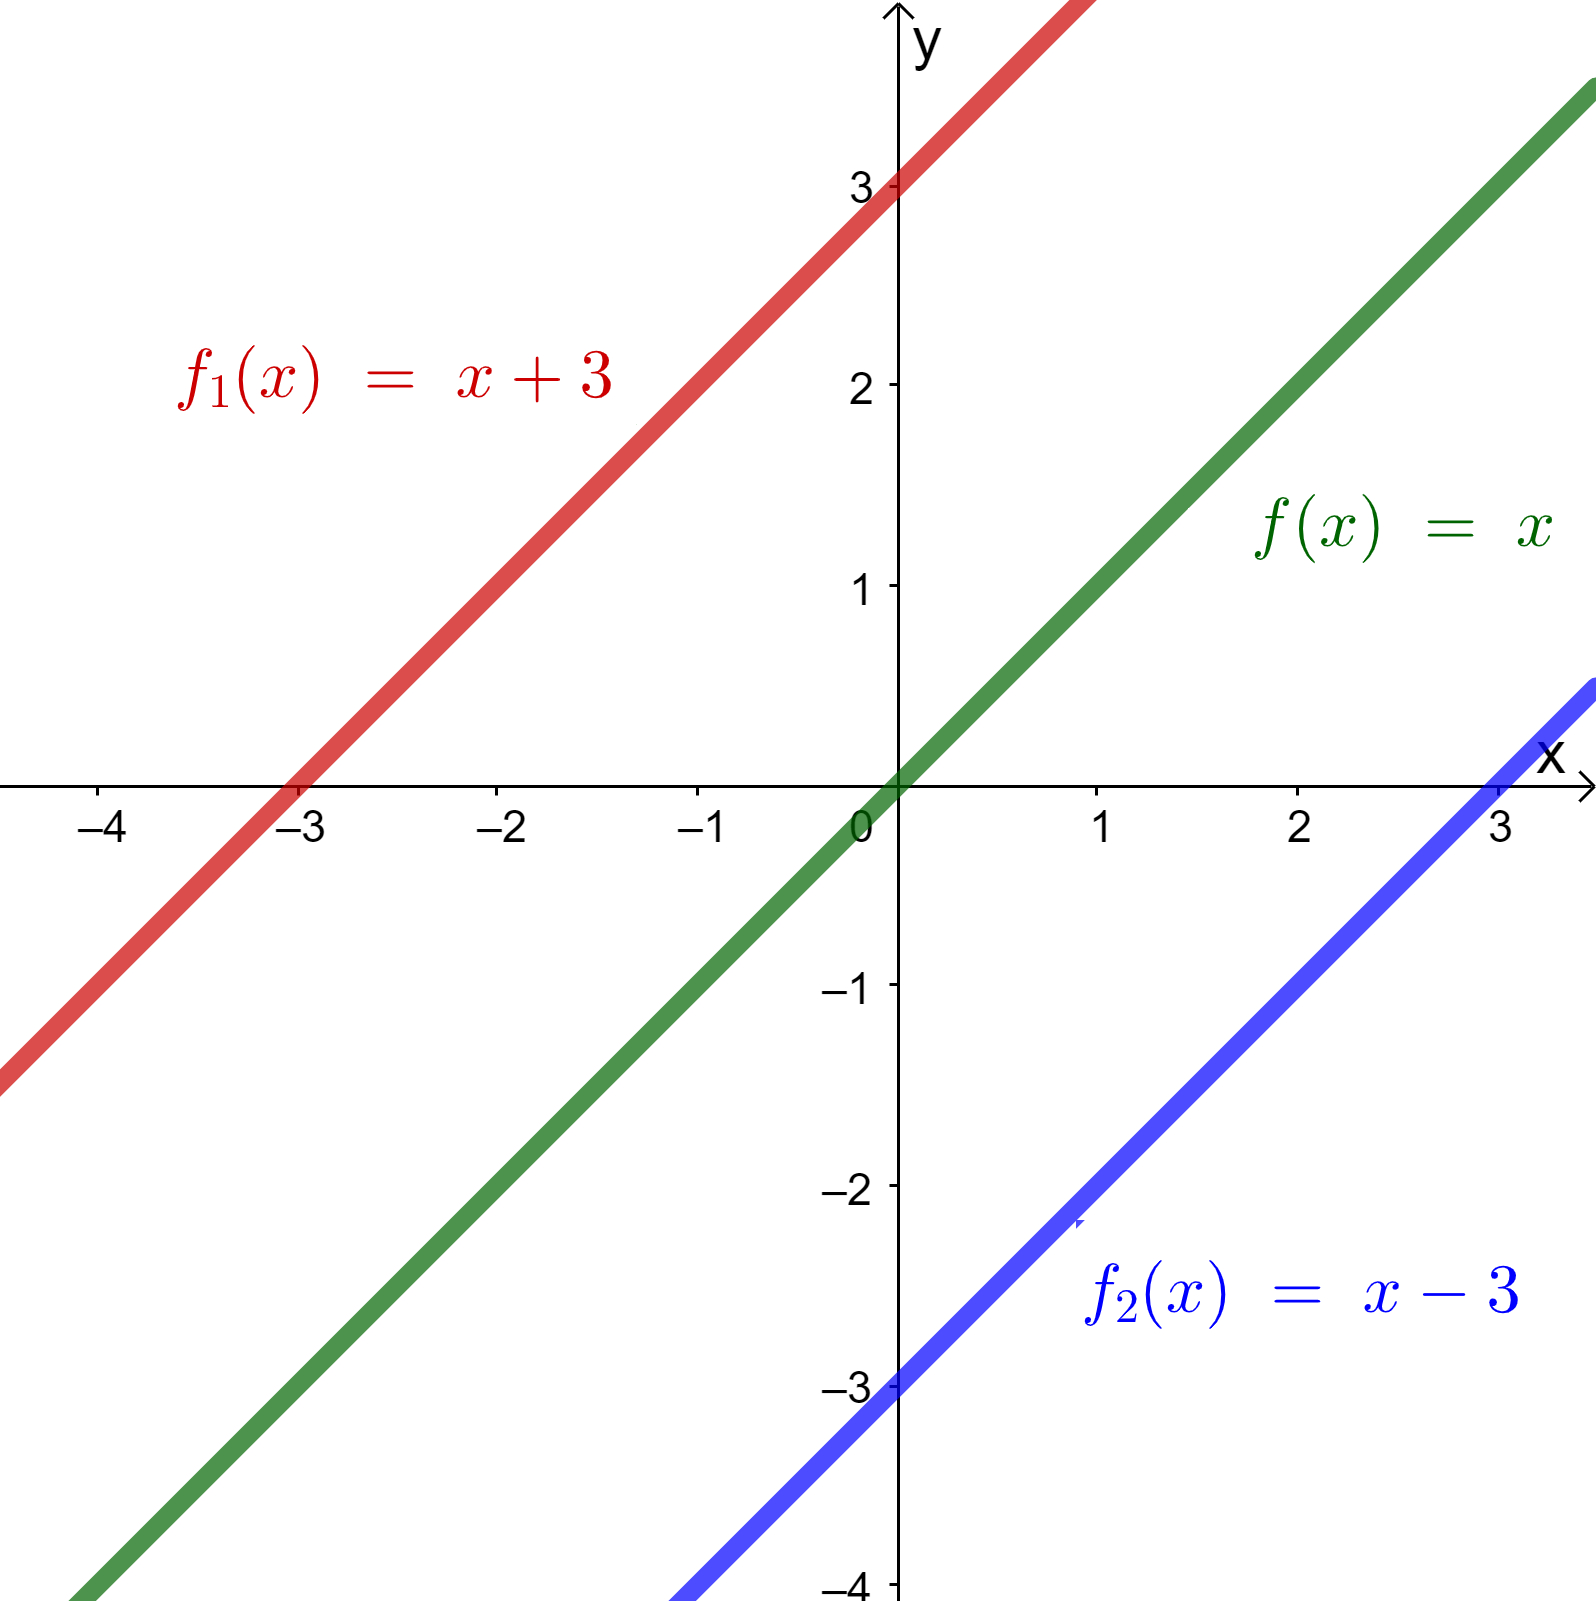
\includegraphics[width=0.95\textwidth]{../Mathematik_1/Bilder/funktionen_vertikale_verschiebung_gerade.png}
    \end{minipage}
    \begin{minipage}{0.6\textwidth}
        \begin{itemize}
            \item Originalfunktion:
            \[
            \textcolor{darkgreen}{f:x\mapsto x}
            \]

            \item Verschiebung um \(3\) Einheiten nach oben:
            \[
            \textcolor{red}{f_1:x\mapsto x+3}
            =
            \textcolor{darkgreen}{f}(x)+3
            \]

            \item Verschiebung um \(3\) Einheiten nach unten:
            \[
            \textcolor{blue}{f_2:x\mapsto x-3}
            =
            \textcolor{darkgreen}{f}(x)-3
            \]
        \end{itemize}
    \end{minipage}
\end{exabox}

Wird der Funktionswert \(f(x)\) mit einer Konstanten \(m\) multipliziert, werden seine Werte und damit ihre Abst�nde von der \(x\)-Achse mit dem Faktor \(|m|\) skaliert.
\begin{itemize}
    \item F�r \(|m|>1\) wird der Graph in vertikaler Richtung gestreckt.
    \item F�r \(0<|m|<1\) wird der Graph in vertikaler Richtung gestaucht.
    \item F�r \(m<0\) erfolgt zus�tzlich eine Spiegelung an der \(x\)-Achse.
\end{itemize}

F�r \(m=0\) werden dagegen alle Funktionswerte auf \(0\) abgebildet; es
entsteht die konstante Nullfunktion.

\begin{exabox}{Vertikale Streckung und Stauchung}{ }
    \begin{minipage}{0.5\textwidth}
        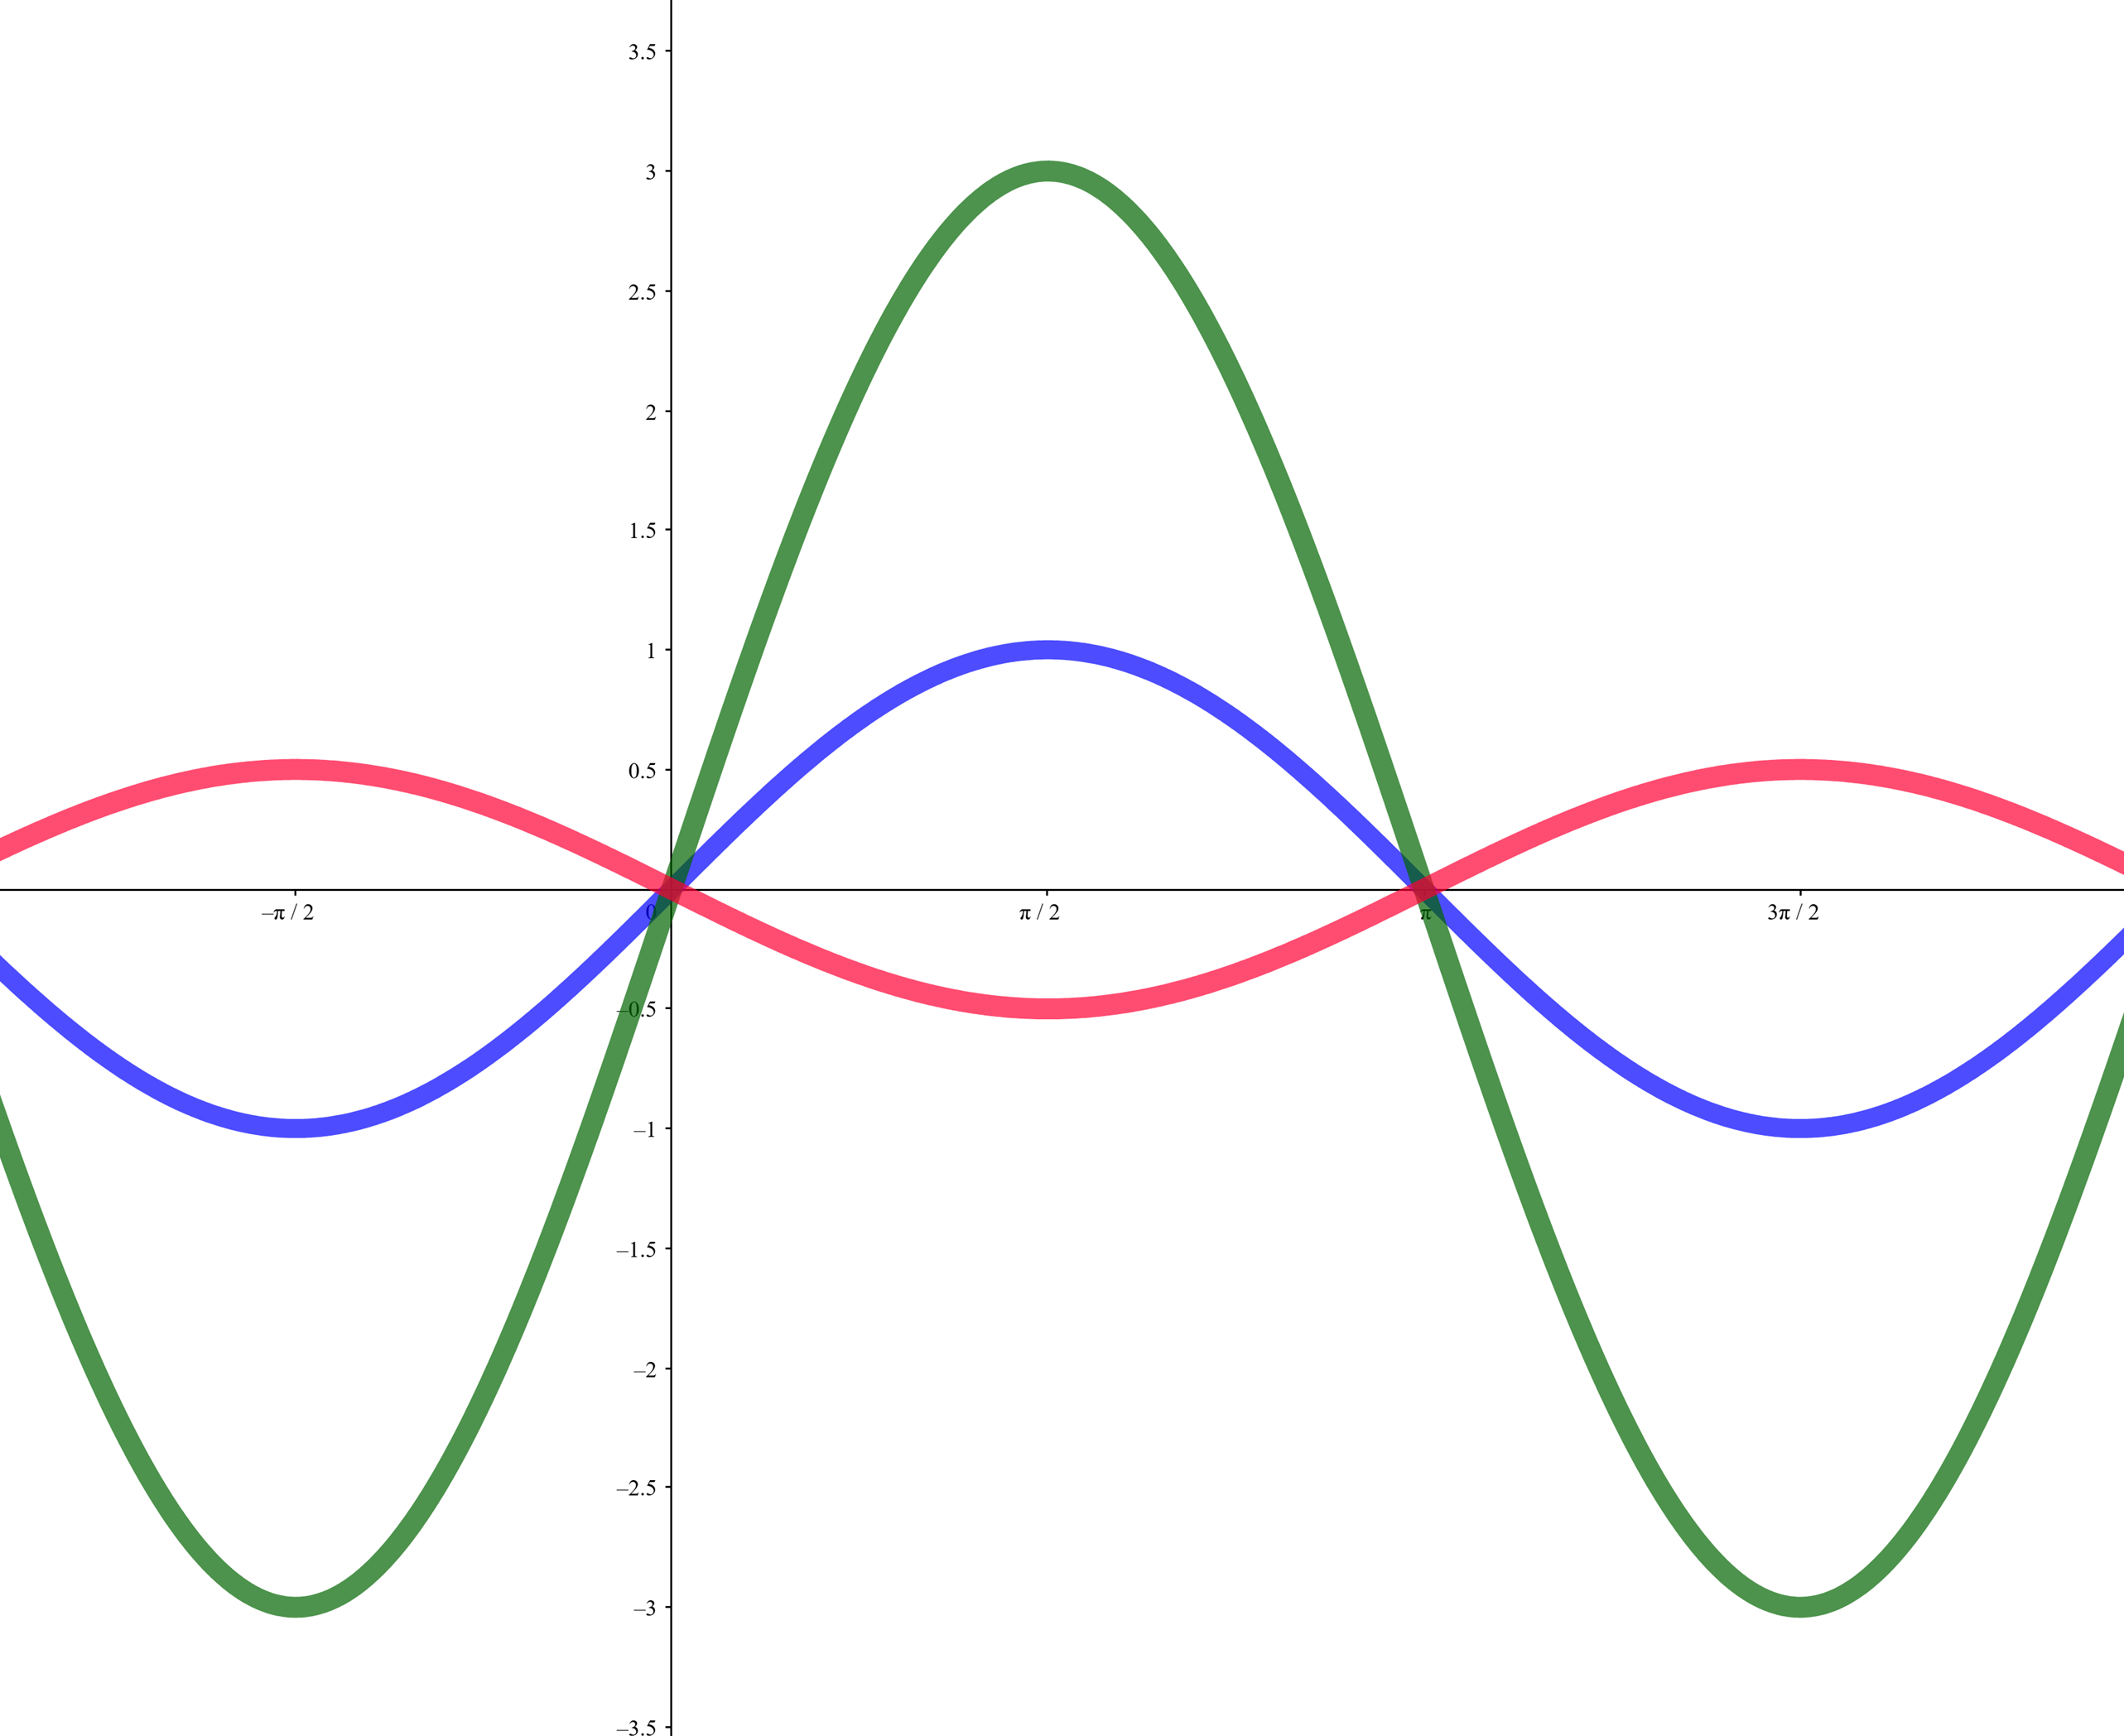
\includegraphics[width=0.95\textwidth]{../Mathematik_1/Bilder/funktionen_vertikale_skalierung_sinus.png}
    \end{minipage}
    \begin{minipage}{0.4\textwidth}
        \begin{itemize}
            \item Originalfunktion:
            \[
            \textcolor{blue}{f:x\mapsto\sin(x)}
            \]

            \item Streckung in \(y\)-Richtung:
            \[
            \textcolor{darkgreen}{f_1:x\mapsto3\sin(x)}
            =
            3\cdot\textcolor{blue}{f}(x)
            \]

            \item Stauchung in \(y\)-Richtung und Spiegelung an der
            \(x\)-Achse:
            \[
            \textcolor{red}{f_2:x\mapsto-\frac12\sin(x)}
            =
            -\frac12\cdot\textcolor{blue}{f}(x)
            \]
        \end{itemize}
    \end{minipage}
\end{exabox}

Beide vertikalen Ver�nderungen lassen sich miteinander kombinieren. F�r
\[
g(y)=my+b
\]
gilt
\[
(g\circ f)(x)=m\,f(x)+b.
\]
Dabei werden die Funktionswerte zun�chst mit \(m\) skaliert und anschlie�end
um \(b\) verschoben.


\subsubsection*{Ver�nderung in horizontaler Richtung}

Wird eine Konstante \(a\) innerhalb des Arguments von \(f\) addiert,
\[
x\mapsto f(x+a),
\]
ver�ndern sich nicht unmittelbar die Funktionswerte, sondern die Stellen,
an denen diese Funktionswerte angenommen werden. Der Graph wird dadurch in
horizontaler Richtung verschoben.

Dabei wirkt das Vorzeichen zun�chst ungewohnt. Angenommen, die urspr�ngliche
Funktion nimmt einen bestimmten Funktionswert an der Stelle \(x_0\) an. Die
ver�nderte Funktion \(f(x+a)\) nimmt denselben Funktionswert genau dann an,
wenn
\[
x+a=x_0.
\]
Daraus folgt
\[
x=x_0-a.
\]
Der urspr�ngliche Punkt wird also um \(a\) Einheiten nach links verschoben.

Damit gilt:
\begin{itemize}
    \item F�r \(a>0\) wird der Graph von \(f(x+a)\) um \(a\) Einheiten nach
          links verschoben.
    \item F�r \(a<0\) erfolgt die Verschiebung entsprechend nach rechts.
\end{itemize}

\begin{exabox}{Horizontale Translation}{ }
    \begin{minipage}{0.5\textwidth}
        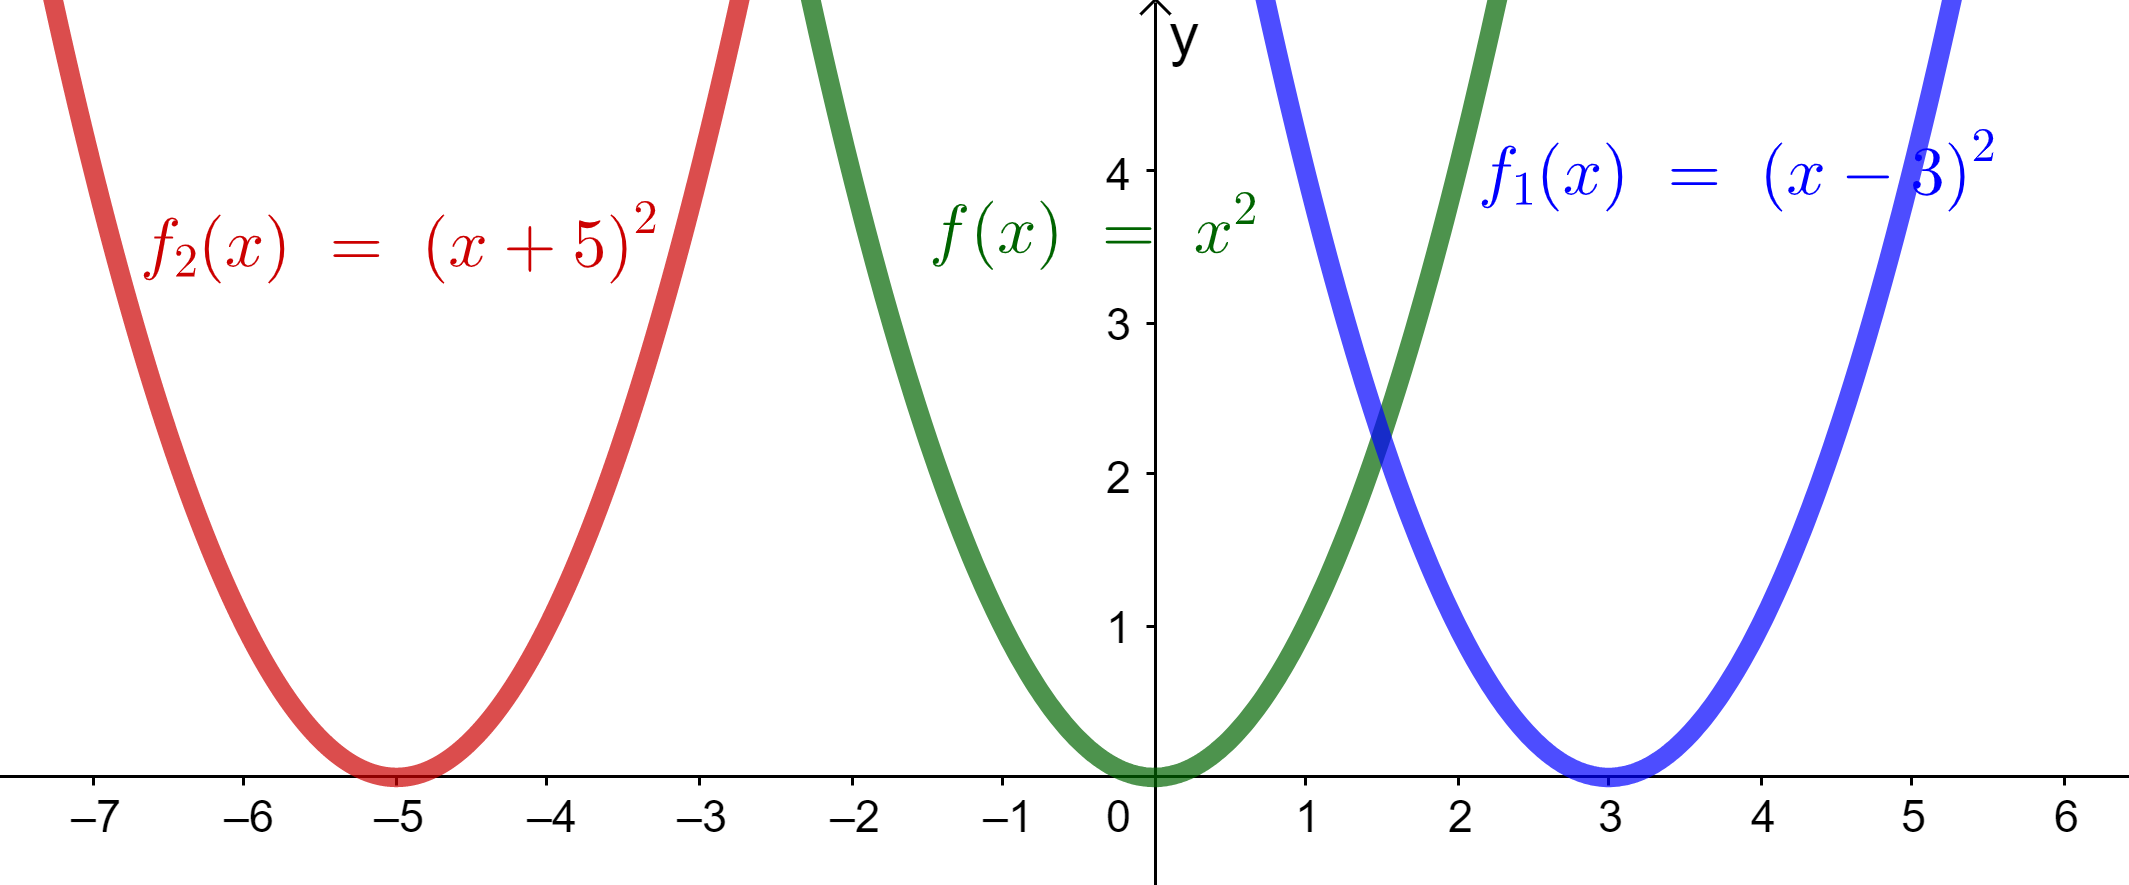
\includegraphics[width=0.95\textwidth]{../Mathematik_1/Bilder/funktionen_horizontale_verschiebung_quadratfunktion.png}
    \end{minipage}
    \begin{minipage}{0.5\textwidth}
        \begin{itemize}
            \item Originalfunktion:
            \[
            \textcolor{darkgreen}{f:x\mapsto x^2}
            \]

            \item Verschiebung um \(3\) Einheiten nach rechts:
            \[
            \textcolor{blue}{f_1:x\mapsto(x-3)^2}
            =
            \textcolor{darkgreen}{f}(x-3)
            \]

            \item Verschiebung um \(5\) Einheiten nach links:
            \[
            \textcolor{red}{f_2:x\mapsto(x+5)^2}
            =
            \textcolor{darkgreen}{f}(x+5)
            \]
        \end{itemize}
    \end{minipage}
\end{exabox}

Auch eine Multiplikation innerhalb des Arguments wirkt horizontal.
Bei
\[
x\mapsto f(kx)
\]
muss f�r einen urspr�nglich an der Stelle \(x_0\) angenommenen Funktionswert
nun
\[
kx=x_0
\]
gelten. Daraus folgt
\[
x=\frac{x_0}{k}.
\]
Die \(x\)-Koordinaten werden also mit dem Faktor \(1/k\) skaliert. Daher gilt:
\begin{itemize}
    \item F�r \(|k|>1\) wird der Graph zur \(y\)-Achse hin gestaucht.
    \item F�r \(0<|k|<1\) wird der Graph von der \(y\)-Achse weg gestreckt.
    \item F�r \(k<0\) erfolgt zus�tzlich eine Spiegelung an der \(y\)-Achse.
\end{itemize}

\begin{exabox}{Horizontale Streckung und Stauchung}{ }
    \begin{minipage}{0.4\textwidth}
        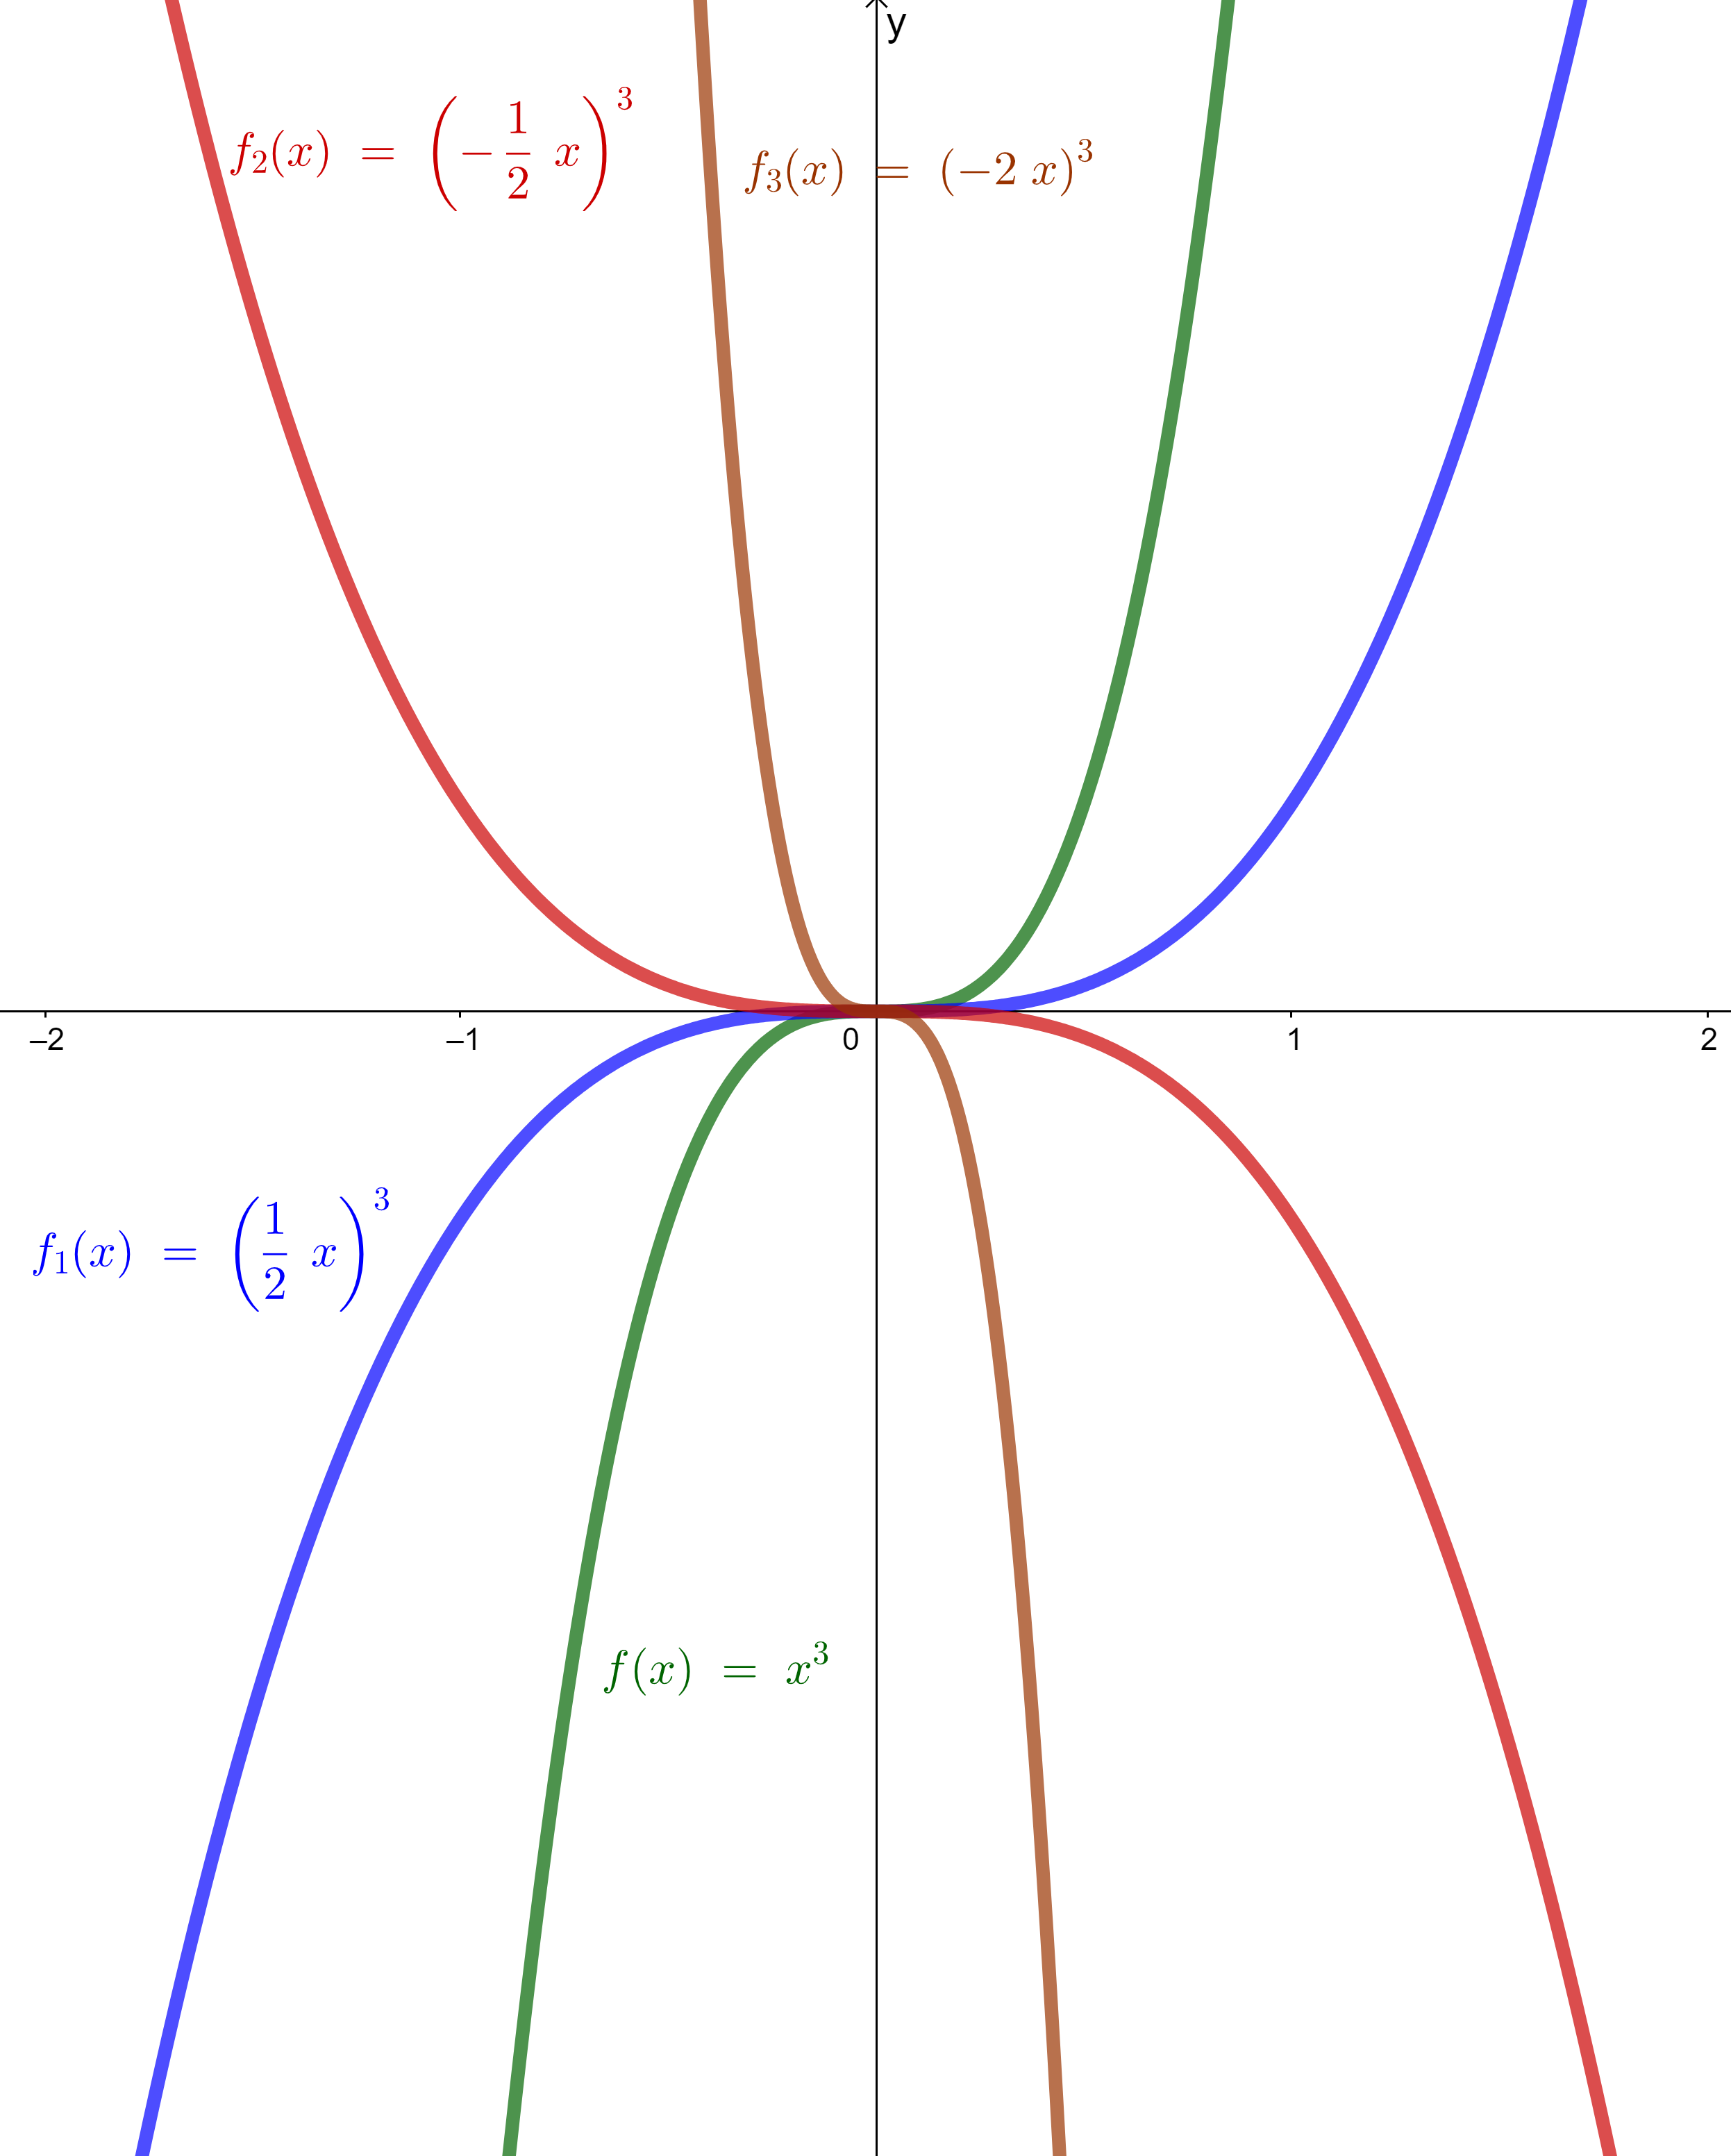
\includegraphics[width=0.95\textwidth]{../Mathematik_1/Bilder/funktionen_horizontale_skalierung_potenz_drei.png}
    \end{minipage}
    \begin{minipage}{0.6\textwidth}
        \begin{itemize}
            \item Originalfunktion:
            \[
            \textcolor{darkgreen}{f:x\mapsto x^3}
            \]

            \item Streckung in \(x\)-Richtung:
            \[
            \textcolor{blue}{
            f_1:x\mapsto
            \left(\frac12x\right)^3}
            =
            \textcolor{darkgreen}{f}\left(\frac12x\right)
            \]

            \item Streckung in \(x\)-Richtung und Spiegelung an der
            \(y\)-Achse:
            \[
            \textcolor{red}{
            f_2:x\mapsto
            \left(-\frac12x\right)^3}
            =
            \textcolor{darkgreen}{f}\left(-\frac12x\right)
            \]

            \item Stauchung in \(x\)-Richtung und Spiegelung an der
            \(y\)-Achse:
            \[
            \textcolor{brown}{
            f_3:x\mapsto(-2x)^3}
            =
            \textcolor{darkgreen}{f}(-2x)
            \]
        \end{itemize}
    \end{minipage}
\end{exabox}

Horizontale Ver�nderungen wirken damit in gewisser Weise umgekehrt zu
vertikalen Ver�nderungen: Ein Faktor mit Betrag gr��er als \(1\) f�hrt
horizontal zu einer Stauchung, ein Faktor mit Betrag kleiner als \(1\) zu
einer Streckung. Auch bei Verschiebungen erscheint das Vorzeichen innerhalb
des Funktionsarguments entgegengesetzt zur geometrischen
Verschiebungsrichtung.

Beide horizontalen Ver�nderungen lassen sich wiederum kombinieren. F�r
\[
g(x)=k(x+a),
\qquad k\neq0,
\]
gilt
\[
(f\circ g)(x)=f\!\bigl(k(x+a)\bigr).
\]

\subsubsection*{Transformationsbaukasten}

Vertikale und horizontale Ver�nderungen k�nnen gleichzeitig auftreten.
Ausgehend von einer Funktion \(f\) lassen sie sich in der Form
\[
F(x)=m\cdot f\!\bigl(k(x+a)\bigr)+b
\]
zusammenfassen.

\begin{theorembox}{Transformations-Baukasten}{ }

F�r
\[
F(x)=m\cdot f\!\bigl(k(x+a)\bigr)+b,
\qquad
m,a,b,k\in\mathbb R,\quad k\neq0,
\]
haben die Parameter folgende geometrische Bedeutung:

\begin{itemize}
		\item \(m\) ver�ndert die Funktionswerte und damit die vertikale Skalierung:
\begin{itemize}
    \item \(|m|>1\): vertikale Streckung,
    \item \(0<|m|<1\): vertikale Stauchung,
    \item \(m<0\): zus�tzliche Spiegelung an der \(x\)-Achse,
    \item \(m=0\): alle Funktionswerte werden auf \(0\) abgebildet.
\end{itemize}

    \item \(b\) verschiebt den Graphen vertikal:
          \begin{itemize}
              \item \(b>0\): nach oben,
              \item \(b<0\): nach unten.
          \end{itemize}

    \item \(k\) ver�ndert das Argument und damit die horizontale Skalierung:
          \begin{itemize}
              \item \(|k|>1\): horizontale Stauchung,
              \item \(0<|k|<1\): horizontale Streckung,
              \item \(k<0\): zus�tzliche Spiegelung an der \(y\)-Achse.
          \end{itemize}

    \item \(a\) verschiebt den Graphen horizontal:
          \begin{itemize}
              \item \(a>0\): um \(a\) Einheiten nach links,
              \item \(a<0\): um \(|a|\) Einheiten nach rechts.
          \end{itemize}
\end{itemize}

Die �u�ere Ver�nderung
\[
y\mapsto my+b
\]
wirkt auf die Funktionswerte und damit in vertikaler Richtung. Die innere
Ver�nderung
\[
x\mapsto k(x+a)
\]
wirkt auf das Argument der Funktion und damit in horizontaler Richtung.

\end{theorembox}


\subsection{Harmonische Schwingungen als Verkn�pfungen}

Die zuvor untersuchten Transformationen k�nnen nun auf die Sinusfunktion angewendet werden. Ausgehend von
\[
t\mapsto\sin(t)
\]
kann das Argument durch
\[
t\mapsto\omega\cdot  t+\varphi_0
\]
ver�ndert werden. Anschlie�end k�nnen die entstehenden Funktionswerte skaliert und verschoben werden:
\[
y\mapsto A\cdot y+d.
\]

Die Verkettung dieser drei Funktionen f�hrt auf eine \emph{harmonische Schwingung}
\[
	s(t)=A\sin(\omega t+\varphi_0)+d\,.
\]
Harmonische Schwingungen treten h�ufig auf und die Parameter besitzten eine klare Bedeutung:

\begin{itemize}
  \item \(A\not=0\) ist die \textbf{Amplitude}. F�r \(A<0\) kommt eine Spiegelung an der horizontalen Mittellinie hinzu.
  \item \(\omega>0\) ist die \textbf{Kreisfrequenz}. Sie bestimmt die \textbf{Periodendauer} \( T=\frac{2\pi}{|\omega|}\).
  \item \(\varphi_0\) ist die \textbf{Nullsphase}. Da \(\omega\neq0\) kann \( \omega t+\varphi_0 = \omega\left(t+\frac{\varphi_0}{\omega}\right) \) geschrieben werden. Dies entspricht einer horizontalen Verschiebung um \( -\frac{\varphi_0}{\omega}\).
  \item \(d\) verschiebt die Schwingung vertikal. Die Gerade \(y=d\) bildet die Mittellinie der Schwingung.
\end{itemize}

\begin{exabox}{Parameter einer harmonischen Schwingung interpretieren}{ }

Betrachtet wird die harmonische Schwingung
\[
s(t)
=
2\sin\left(3t-\frac{\pi}{2}\right)+1.
\]

Um die geometrische Bedeutung der einzelnen Parameter zu erkennen, wird die
Funktion mit der allgemeinen Form
\[
s(t)
=
A\sin(\omega t+\varphi_0)+d
\]
verglichen.

F�r die Amplitude gilt
\[
A=2.
\]
Die Schwingung besitzt daher die \textbf{Amplitude}
\[
|A|=2.
\]
Ausgehend von der Mittellinie liegen die gr��ten und kleinsten Funktionswerte
somit jeweils \(2\) Einheiten entfernt.

Die Kreisfrequenz betr�gt
\[
\omega=3.
\]
Damit ergibt sich die Periodendauer zu
\[
T
=
\frac{2\pi}{\omega}
=
\frac{2\pi}{3}.
\]
Nach einer Zeitspanne von \(2\pi/3\) wiederholt sich die Schwingung.

F�r die horizontale Verschiebung wird das Argument der Sinusfunktion
umgeformt:
\[
3t-\frac{\pi}{2}
=
3\left(t-\frac{\pi}{6}\right).
\]
Die Funktion kann daher auch in der Form
\[
s(t)
=
2\sin\left(
3\left(t-\frac{\pi}{6}\right)
\right)+1
\]
geschrieben werden. Der Graph der Sinusfunktion ist somit um
\[
\frac{\pi}{6}
\]
nach rechts verschoben.

Schlie�lich gilt
\[
d=1.
\]
Die gesamte Schwingung ist daher um eine Einheit nach oben verschoben. Ihre
Mittellinie ist
\[
y=1.
\]

Damit lassen sich die charakteristischen Eigenschaften der Schwingung
zusammenfassen:
\[
\begin{aligned}
\text{Amplitude:}\qquad &2,\\
\text{Periodendauer:}\qquad &\frac{2\pi}{3},\\
\text{horizontale Verschiebung:}\qquad &\frac{\pi}{6}\text{ nach rechts},\\
\text{Mittellinie:}\qquad &y=1.
\end{aligned}
\]

Aus der Mittellinie \(y=1\) und der Amplitude \(2\) folgen au�erdem unmittelbar
der maximale und der minimale Funktionswert:
\[
s_{\max}=1+2=3,
\qquad
s_{\min}=1-2=-1.
\]

Das Beispiel zeigt, wie die Parameter einer harmonischen Schwingung
systematisch aus ihrer Funktionsgleichung gelesen und als Ver�nderungen der
Grundfunktion \(t\mapsto \sin(t)\) interpretiert werden k�nnen.

\end{exabox}

\noindent \textbf{Merke:} 
Das Beispiel der harmonischen Schwingung zeigt, wie aus einer einfachen
Grundfunktion durch Verkettungen eine andere Funktion entsteht.

Die Verkettung von Funktionen ist damit nicht nur eine formale Operation.
Sie erm�glicht, komplexere Funktionen aus einfachen Grundfunktionen
systematisch aufzubauen und die Wirkung einzelner Parameter auf den
Funktionsgraphen zu verstehen. Diese Sichtweise wird sp�ter insbesondere bei
der Differentialrechnung wieder wichtig, wenn verkettete Funktionen mithilfe
der Kettenregel abgeleitet werden.

 % Komposition von Funktionen (mit Bezug zu Schwingungen)

\chapter{Komplexe Zahlen}
\etocsettocstyle{\section*{Inhalt dieses Kapitels}}{}
\section*{Leitidee}

Die reellen Zahlen reichen nicht aus, um jede algebraische Gleichung zu
l�sen. Bereits die einfache Gleichung
\[
x^2=-1
\]
besitzt keine reelle L�sung. Die Einf�hrung der \textbf{komplexen Zahlen}
(\emph{complex numbers}) erweitert den bisherigen Zahlenbereich so, dass auch
solche Gleichungen sinnvoll behandelt werden k�nnen.

Komplexe Zahlen verbinden dabei mehrere mathematische Perspektiven. In
\textbf{kartesischer Darstellung} erscheinen sie als Zahlen der Form
\[
	z=x+ i \, y
\]
und k�nnen geometrisch als Punkte oder Zeiger in der komplexen Ebene
interpretiert werden. Dadurch erhalten auch algebraische Operationen eine
geometrische Bedeutung.

Eine zweite Darstellung entsteht durch Betrag und Winkel. Diese
\textbf{Polarform} beschreibt eine komplexe Zahl durch ihre L�nge und ihre
Richtung. Mithilfe der komplexen Exponentialfunktion f�hrt sie auf die
Darstellung
\[
	z=r\,e^{i\,\varphi}.
\]
Insbesondere Multiplikation, Division, Potenzieren und Wurzelziehen erhalten
dadurch eine besonders anschauliche und zugleich rechnerisch g�nstige Form.

Die Verbindung zur Exponentialfunktion f�hrt schlie�lich unmittelbar zu
periodischen Vorg�ngen. Die komplexe Exponentialfunktion beschreibt eine
Drehbewegung in der komplexen Ebene und bildet damit die Grundlage der
\textbf{Zeigerdarstellung} harmonischer Schwingungen. Amplitude und Phase
werden dabei durch Betrag und Winkel einer komplexen Zahl beschrieben.
�berlagerung, Ableitung und Integration harmonischer Schwingungen k�nnen auf
diese Weise auf algebraische Operationen mit komplexen Zahlen zur�ckgef�hrt
werden.

Die Verbindung von algebraischer Erweiterung, geometrischer Interpretation
und analytischer Darstellung macht die komplexen Zahlen zu einem
grundlegenden Werkzeug f�r die Beschreibung periodischer und dynamischer
Prozesse.

  % Leitidee Komplexe Zahlen

\bigskip
\localtableofcontents
\newpage


\setcounter{satz}{0} \setcounter{def}{0} \setcounter{exa}{0}  \section{Komplexe Zahlen I: Zahl, Ebene und Rechnen}\label{MA1-komplexe-zahlen-grundlagen}

\begin{table}[H]
  \centering
  \begin{tabularx}{\textwidth}{p{0.9\textwidth} p{0.1\textwidth}}
    \toprule
    \multicolumn{2}{c}{\textbf{�bersicht �ber Lernziele und Voraussetzungen}}\\
    \midrule
    \textbf{Lernziele} &\\[.5\normalbaselineskip]
    \tabitem erkl�ren, warum zur L�sung bestimmter Gleichungen die komplexen Zahlen eingef�hrt werden &\\
    \tabitem komplexe Zahlen in der Form \(z=a+i\,b\) darstellen und ihre Bestandteile bestimmen &\\
    \tabitem Realteil, Imagin�rteil, komplex Konjugiertes und Betrag einer komplexen Zahl bestimmen und geometrisch interpretieren &\\
    \tabitem komplexe Zahlen als Punkte oder Pfeile in der Gau�schen Zahlenebene interpretieren &\\
    \tabitem zwischen kartesischer Darstellung und Polarkoordinaten einer komplexen Zahl wechseln &\\
    \tabitem komplexe Zahlen addieren, subtrahieren, multiplizieren und dividieren &\\
    \tabitem die geometrische Bedeutung der Grundrechenarten als Pfeiladdition, Skalierung und Drehung erkl�ren &\\[.5\normalbaselineskip]
    \midrule
    \textbf{Voraussetzungen} &\\[.5\normalbaselineskip]
    \tabitem algebraische Gleichungen und �quivalenzumformungen & \abschnittsverweis{MA1-algebraische-gleichungen}\\
    \tabitem Satz des Pythagoras und trigonometrische Funktionen & \abschnittsverweis{MA1-trigonometrische-funktionen}\\
    \tabitem kartesische Koordinaten und Polarkoordinaten & \abschnittsverweis{MA1-trigonometrische-funktionen}\\
    \bottomrule
  \end{tabularx}
\end{table}

\ifintegriereaufgaben
\noindent �bungsaufgaben zu diesem Abschnitt:
\hyperref[MA1-komplexe-zahlen-grundlagen-aufgaben]{Aufgaben}
\vspace{0.3cm}
\hrule
\fi


\subsection{Warum komplexe Zahlen?}

Die bisher betrachteten Zahlenmengen sind im Verlauf der Mathematik immer
wieder erweitert worden. In den nat�rlichen Zahlen ist beispielsweise die
Subtraktion nicht uneingeschr�nkt m�glich; die ganzen Zahlen schlie�en diese
L�cke. In den ganzen Zahlen ist die Division nicht uneingeschr�nkt m�glich;
die rationalen Zahlen erweitern den Zahlenbereich entsprechend. Die reellen
Zahlen erm�glichen schlie�lich unter anderem die Beschreibung irrationaler
Gr��en wie \(\sqrt{2}\).

Auch innerhalb der reellen Zahlen bleiben jedoch Gleichungen �brig, die keine
L�sung besitzen. Das einfachste Beispiel ist
\[
x^2=-1.
\]
F�r jede reelle Zahl \(x\) gilt
\[
x^2\geq0.
\]
Daher kann keine reelle Zahl die Gleichung \(x^2=-1\) erf�llen.

Um auch solche Gleichungen behandeln zu k�nnen, wird der Zahlenbereich erneut
erweitert.

\begin{defbox}{Imagin�re Einheit}{ }

Die \textbf{imagin�re Einheit} (\emph{imaginary unit}) \(i\) ist durch
\[
i^2=-1
\]
definiert.

Damit besitzt die Gleichung
\[
x^2=-1
\]
in den komplexen Zahlen die beiden L�sungen
\[
x=\pm i.
\]

\end{defbox}

In der Elektrotechnik wird f�r die imagin�re Einheit h�ufig \(j\) anstelle
von \(i\) verwendet, da \(i\) dort �blicherweise die elektrische Stromst�rke
bezeichnet.

Eine \textbf{komplexe Zahl} (\emph{complex number}) entsteht, indem zu einer
reellen Zahl ein reelles Vielfaches der imagin�ren Einheit addiert wird:
\[
z=a+i\,b,
\qquad
a,b\in\mathbb R.
\]

Die Menge aller komplexen Zahlen wird mit
\[
\mathbb C
=
\{a+i\,b:a,b\in\mathbb R\}
\]
bezeichnet.

F�r \(b=0\) ergibt sich
\[
z=a+i\cdot0=a.
\]
Jede reelle Zahl ist damit zugleich eine komplexe Zahl. Es gilt also
\[
\mathbb R\subset\mathbb C.
\]
Die komplexen Zahlen ersetzen die reellen Zahlen somit nicht, sondern
erweitern den bisherigen Zahlenbereich.

\begin{exabox}{Beispiele komplexer Zahlen}{ }

Beispielsweise gilt
\[
\left\{
1+3i,\;
\sqrt7-91i,\;
3\pi i,\;
0,\;
\pi+\frac{71}{13}i
\right\}
\subset\mathbb C.
\]

Dabei sind auch rein reelle Zahlen wie \(0\) sowie rein imagin�re Zahlen wie
\(3\pi i\) komplexe Zahlen.

\end{exabox}

Die Einf�hrung der komplexen Zahlen erm�glicht insbesondere die L�sung
quadratischer Gleichungen, deren Diskriminante negativ ist. Ein einfaches
Beispiel zeigt, wie komplexe L�sungen dabei entstehen.

\begin{exabox}{Eine quadratische Gleichung mit komplexen L�sungen}{ }

Betrachtet wird die Gleichung
\[
x^2-4x+5=0.
\]

Durch quadratische Erg�nzung ergibt sich
\[
\begin{array}{crcl}
                  & x^2-4x+5       &=& 0\\
\Leftrightarrow   & x^2-4x+4-4+5   &=& 0\\
\Leftrightarrow   & (x-2)^2+1      &=& 0\\
\Leftrightarrow   & (x-2)^2        &=& -1.
\end{array}
\]

Mit
\[
i^2=-1
\]
folgt
\[
x-2=\pm i
\]
und damit
\[
x_{1,2}=2\pm i.
\]

Die Gleichung besitzt keine reellen L�sungen, wohl aber die beiden komplexen
L�sungen
\[
2+i
\qquad\text{und}\qquad
2-i.
\]

\end{exabox}

\noindent\textbf{Bemerkung:}
In der Praxis kann eine quadratische Gleichung nat�rlich weiterhin mit der
allgemeinen L�sungsformel gel�st werden. Ist die \underline{Diskriminante}\randverweis{MA1-algebraische-gleichungen} negativ, f�hrt die auftretende Wurzel einer negativen Zahl auf komplexe L�sungen. Die
quadratische Erg�nzung im vorangegangenen Beispiel macht dagegen besonders
deutlich, an welcher Stelle die imagin�re Einheit \(i\) ben�tigt wird.


\subsection{Bausteine einer komplexen Zahl}

Eine komplexe Zahl
\[
z=a+i\,b
\]
besteht aus zwei reellen Komponenten. Die Zahl \(a\) beschreibt den reellen
Anteil, die Zahl \(b\) den Koeffizienten der imagin�ren Einheit.

\begin{defbox}{Grundbegriffe und Notationen}{ }

F�r
\[
z=a+i\,b,
\qquad a,b\in\mathbb R,
\]
gelten folgende Bezeichnungen:

\begin{itemize}
    \item Der \textbf{Realteil} (\emph{real part}) von \(z\) ist
    \[
    \mathrm{Re}(z)=a.
    \]

    \item Der \textbf{Imagin�rteil} (\emph{imaginary part}) von \(z\) ist
    \[
    \mathrm{Im}(z)=b.
    \]

    \item Die \textbf{komplex konjugierte Zahl}
    (\emph{complex conjugate}) zu \(z\) ist
    \[
    \overline z=a-i\,b.
    \]

    \item Der \textbf{Betrag} (\emph{magnitude}) von \(z\) ist
    \[
    |z|
    =
    \sqrt{a^2+b^2}.
    \]
\end{itemize}

\end{defbox}

Die Begriffe lassen sich unmittelbar an einer konkreten komplexen Zahl ablesen.

\begin{exabox}{Realteil, Imagin�rteil, Konjugation und Betrag}{ }

\begin{minipage}{0.3\textwidth}
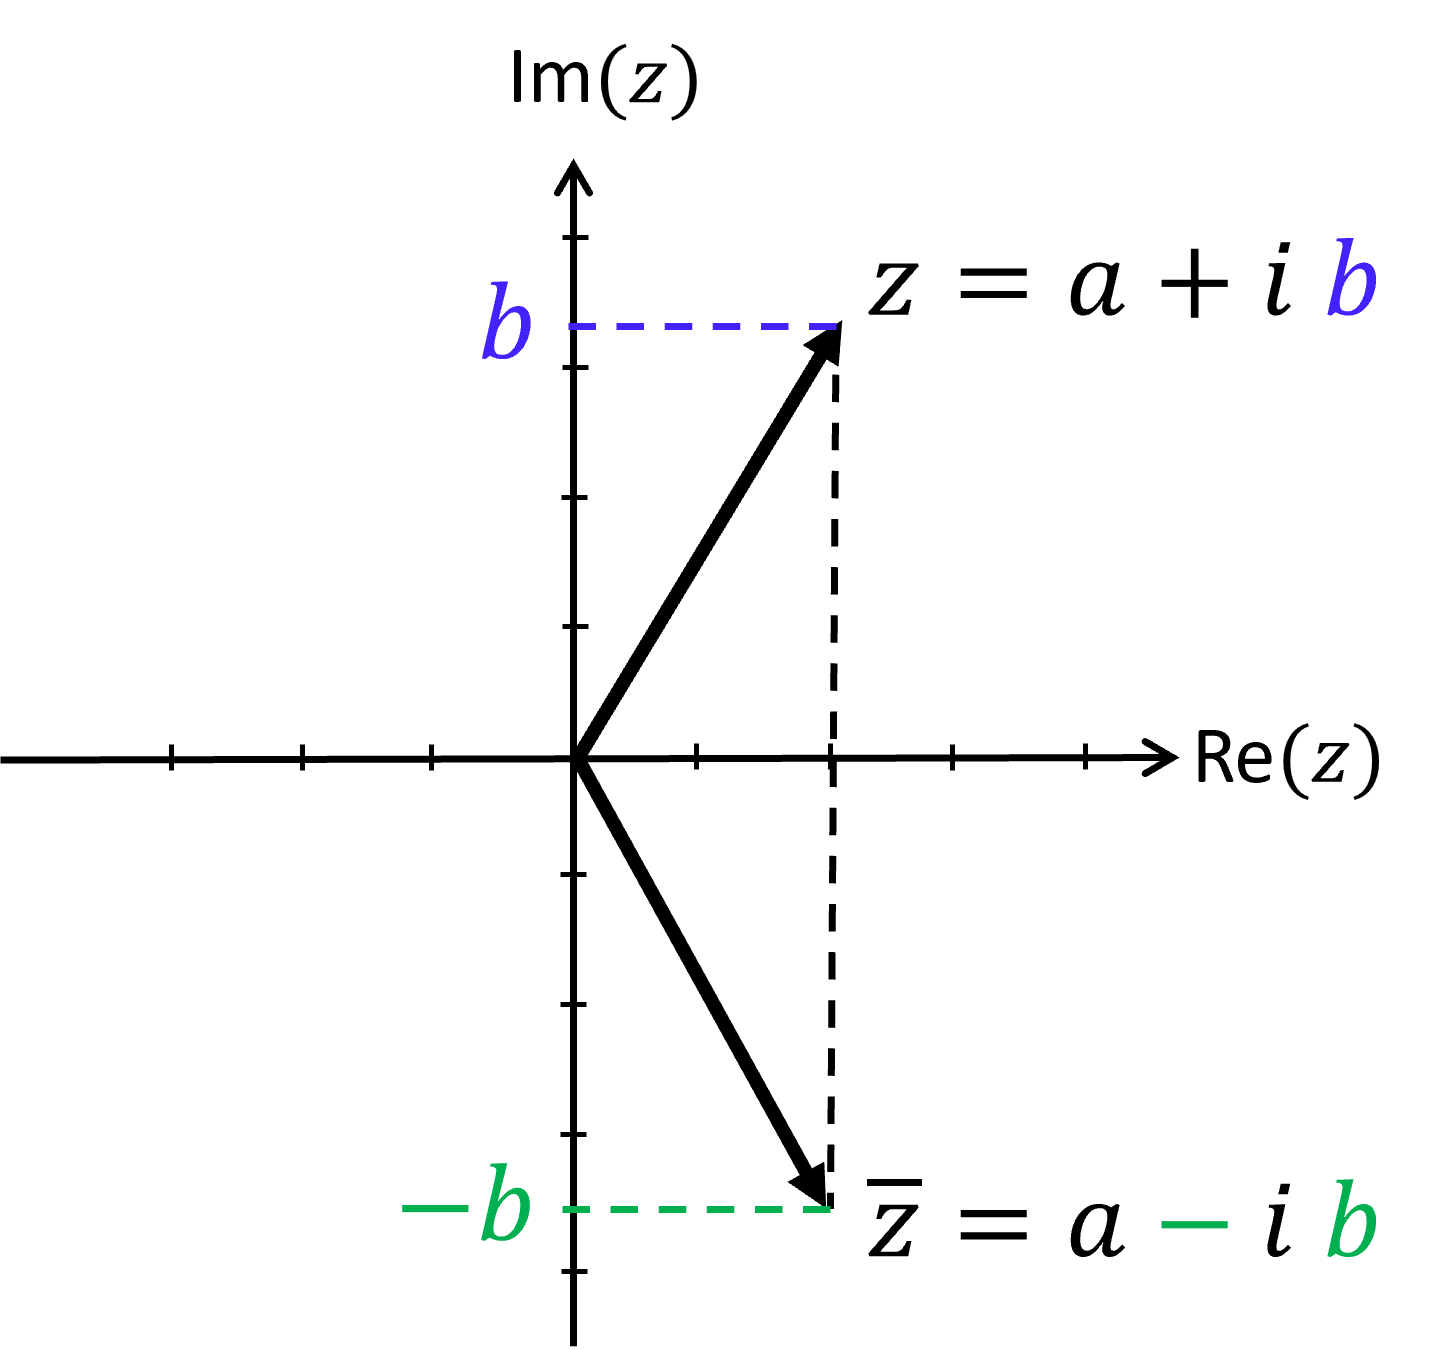
\includegraphics[width=\textwidth]{../Mathematik_1/Bilder/komplexe_zahlen_konjugation_spiegelung.png}
\end{minipage}
\begin{minipage}{0.68\textwidth}


F�r
\[
z=3+4i
\]
gilt
\[
\mathrm{Re}(z)=3
\qquad\text{und}\qquad
\mathrm{Im}(z)=4.
\]

Die komplex konjugierte Zahl lautet
\[
\overline z=3-4i.
\]

F�r den Betrag ergibt sich
\[
|z|
=
\sqrt{(\mathrm{Re}(z))^2+(\mathrm{Im}(z))^2}
=
\sqrt{3^2+4^2}
=
\sqrt{25}
=
5.
\]
\end{minipage}

\end{exabox}

Zwischen diesen Begriffen bestehen einige wichtige Zusammenh�nge. F�r
\[
z=a+i\,b
\]
gilt zun�chst
\[
|z|\geq0
\]
und
\[
|z|=0
\quad\Longleftrightarrow\quad
z=0.
\]

Ist \(z\) reell, also \(b=0\), so ergibt sich
\[
|z|
=
\sqrt{a^2}
=
|a|.
\]
Der Betrag einer komplexen Zahl erweitert damit den bereits bekannten
Absolutbetrag reeller Zahlen.

Besonders wichtig ist das Produkt einer komplexen Zahl mit ihrer konjugierten
Zahl:
\[
z\overline z
=
(a+i\,b)\cdot (a-i\,b)
=
a^2-i\, a\cdot b+i\, a\cdot b-i^2\cdot b^2
=
a^2+b^2
=
|z|^2.
\]
Damit gilt
\[
z\overline z=|z|^2
\]
und entsprechend
\[
|z|=\sqrt{z\overline z}.
\]

Au�erdem gilt
\[
z+\overline z=2\,\mathrm{Re}(z)
\]
sowie
\[
z-\overline z=2i\,\mathrm{Im}(z).
\]

Die algebraischen Begriffe erhalten eine besonders anschauliche Bedeutung,
sobald komplexe Zahlen geometrisch dargestellt werden.


\subsection{Die Gau�sche Zahlenebene}

Eine komplexe Zahl
\[
z=a+i\,b
\]
wird durch zwei reelle Zahlen \(a\) und \(b\) bestimmt. Daher liegt es nahe,
sie mit einem Punkt
\[
(a,b)\in\mathbb R^2
\]
zu identifizieren.

Im Zusammenhang mit komplexen Zahlen wird dieses Koordinatensystem als
\textbf{Gau�sche Zahlenebene} (\emph{complex plane}) bezeichnet. Die
horizontale Achse stellt den Realteil, die vertikale Achse den Imagin�rteil
dar.

Eine komplexe Zahl kann dabei entweder als Punkt oder als Pfeil vom Ursprung
zu diesem Punkt aufgefasst werden:
\[
z=a+i\,b
\quad\widehat=\quad
(a\,|\,b).
\]

\begin{theorembox}{Kartesische Darstellung}{ }

\begin{minipage}{0.3\textwidth}
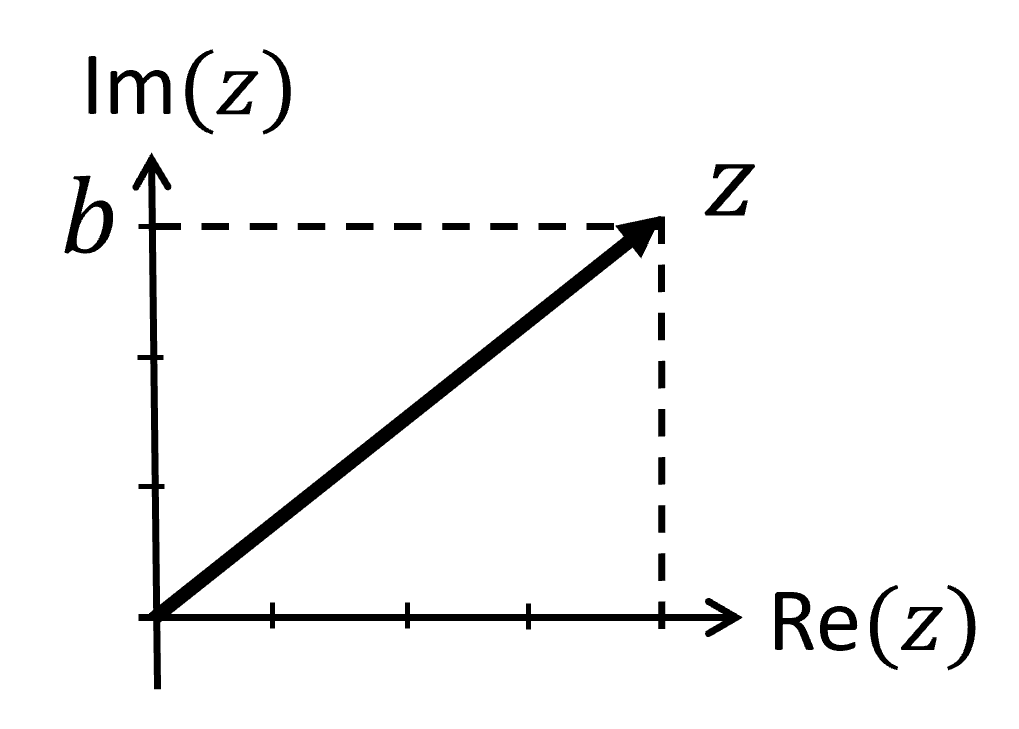
\includegraphics[width=\textwidth]{../Mathematik_1/Bilder/komplexe_zahlen_kartesische_koordinaten.png}
\end{minipage}
\begin{minipage}{0.68\textwidth}

F�r
\[
z=a+i\,b
\]
gilt
\[
z\;\widehat=\;(a\,|\,b),
\]
wobei
\[
a=\mathrm{Re}(z),
\qquad
b=\mathrm{Im}(z).
\]

Der zugeh�rige Pfeil beginnt im Ursprung und endet im Punkt
\[
(a\,|\,b).
\]

\end{minipage}

\end{theorembox}

Durch diese Darstellung erhalten auch die zuvor eingef�hrten Begriffe eine
geometrische Bedeutung.

Der Betrag
\[
|z|=\sqrt{a^2+b^2}
\]
ist nach dem Satz des Pythagoras gerade die L�nge des Pfeils vom Ursprung zum
Punkt \((a\,|\,b)\).

Die komplex konjugierte Zahl
\[
\overline z=a-i\,b
\]
entspricht dem Punkt
\[
(a\,|\,-b).
\]
Die komplexe Konjugation spiegelt den zu \(z\) geh�renden Punkt beziehungsweise
Pfeil daher an der reellen Achse.


\subsubsection*{Polarkoordinaten einer komplexen Zahl}

Die kartesischen Koordinaten beschreiben eine komplexe Zahl durch ihre
horizontale und vertikale Komponente. Derselbe Pfeil kann jedoch auch durch
seine L�nge und seine Richtung beschrieben werden.

Dazu werden der Betrag
\[
r=|z|
\]
und ein Winkel \(\varphi\) verwendet, den der Pfeil mit der positiven reellen
Achse einschlie�t. Diese Beschreibung f�hrt auf die
\textbf{Polarkoordinaten} einer komplexen Zahl.

\begin{theorembox}{Polarkoordinaten}{ }

\begin{minipage}{0.3\textwidth}
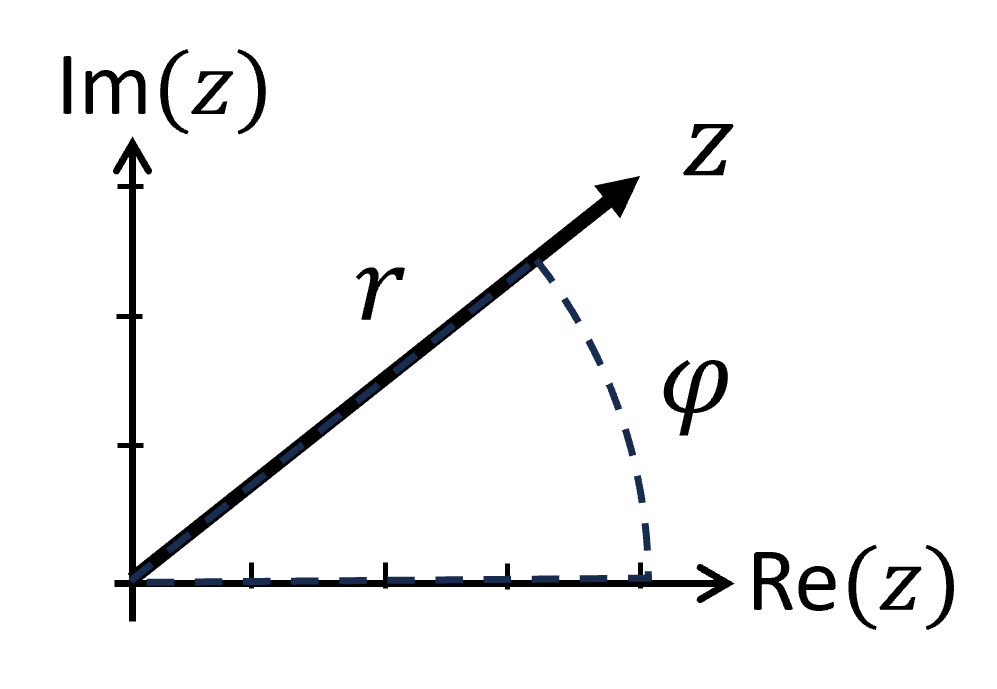
\includegraphics[width=\textwidth]{../Mathematik_1/Bilder/komplexe_zahlen_polarkoordinaten.png}
\end{minipage}
\begin{minipage}{0.7\textwidth}

F�r eine komplexe Zahl \(z\neq0\) gilt
\[
z\;\widehat=\;(r\,|\,\varphi), \quad 
\]
wobei
	\begin{itemize}
		\item \( r=|z|>0 \) die L�nge des Pfils und 
		\item \( \varphi=\arg(z) \) der Winkel zwischen Pfeil und positiven reellen Achse ist.
	\end{itemize}

\end{minipage}

\end{theorembox}

Der Winkel einer komplexen Zahl ist grunds�tzlich nur bis auf ganzzahlige
Vielfache von \(2\pi\) bestimmt. Die Winkel
\[
\varphi_k
=
\varphi+2\pi k,
\qquad k\in\mathbb Z,
\]
beschreiben daher dieselbe Richtung und somit dieselbe komplexe Zahl. Im Folgenden bezeichnet
\[
\arg(z)\in(-\pi,\pi]
\]
den gew�hlten Hauptwert des Arguments.


F�r \(z=0\) gilt zwar \(|z| = 0\), ein Winkel ist jedoch nicht eindeutig bestimmt. Das Argument von \(0\) ist daher nicht definiert.


\subsubsection*{Von Polarkoordinaten zur kartesischen Darstellung}

Sind Betrag \(r\) und Winkel \(\varphi\) gegeben, ergeben sich die
kartesischen Koordinaten unmittelbar aus der Geometrie des zugeh�rigen
rechtwinkligen Dreiecks:
\[
a=r\cos(\varphi)
\]
und
\[
b=r\sin(\varphi).
\]

Damit gilt
\[
z
=
r\cos(\varphi)
+
i\,r\sin(\varphi).
\]

Durch Ausklammern von \(r\) erh�lt man die besonders wichtige Darstellung
\[
z
=
r\bigl(\cos(\varphi)+i\sin(\varphi)\bigr).
\]

Diese Form wird im folgenden Abschnitt eine zentrale Rolle spielen, wenn die
trigonometrische Darstellung mit der komplexen Exponentialfunktion verbunden
wird.


\subsubsection*{Von der kartesischen Darstellung zu Polarkoordinaten}

Ist dagegen \( z = a + i\, b\) gegeben, so liefert der Satz des Pythagoras zun�chst den Betrag:
\[
r
=
|z|
=
\sqrt{a^2+b^2}.
\]

F�r den Winkel m�ssen beide kartesischen Koordinaten ber�cksichtigt werden.
Die Funktion
\[
\operatorname{atan2}(b,a)
\]
liefert den Winkel unter Ber�cksichtigung des Quadranten. F�r \(z\neq0\) gilt
daher
\[
\varphi
=
\operatorname{atan2}(b,a)
\in(-\pi,\pi].
\]

Damit lautet die Umrechnung insgesamt
\[
a+i\,b
\quad\longleftrightarrow\quad
\left(
\sqrt{a^2+b^2}
\,\middle|\,
\operatorname{atan2}(b,a)
\right).
\]

\begin{theorembox}{Kartesisch \(\leftrightarrow\) Polar}{ }

\begin{minipage}{0.3\textwidth}
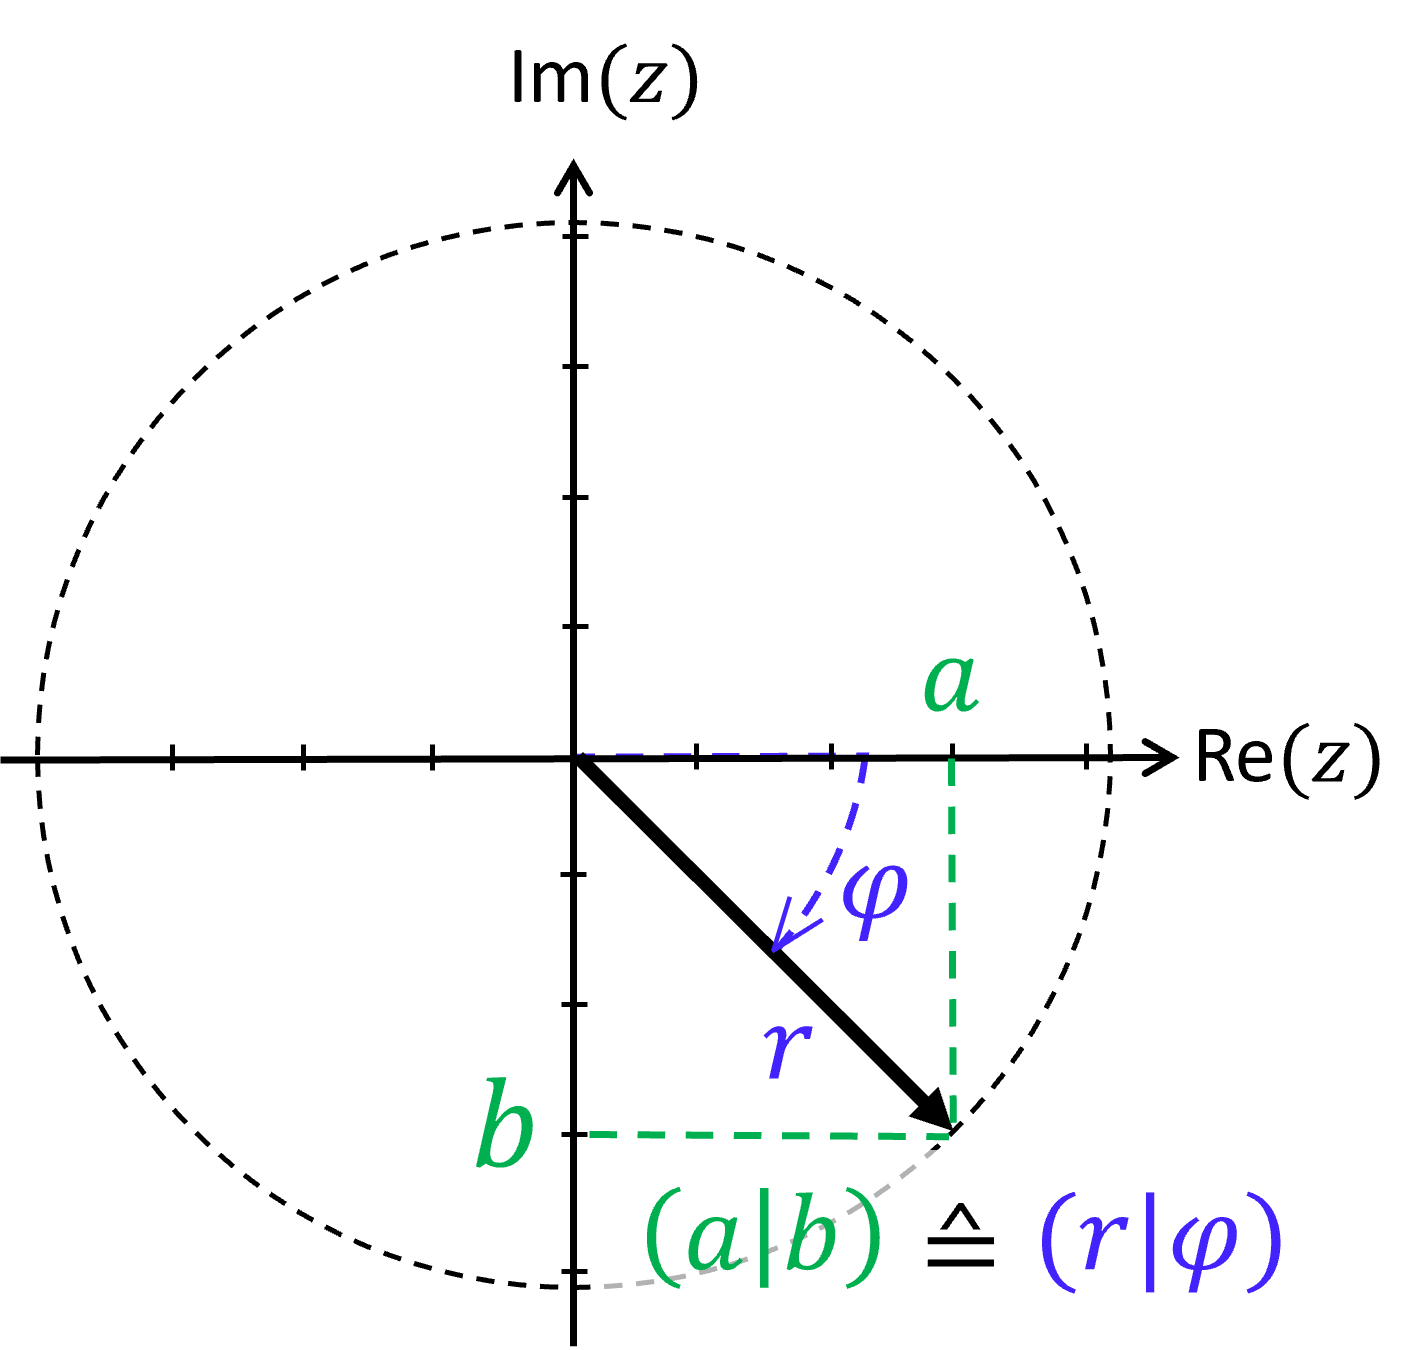
\includegraphics[width=0.8\textwidth]{../Mathematik_1/Bilder/komplexe_zahlen_kartesisch_polar_vierter_quadrant.png}
\end{minipage}
\begin{minipage}{0.7\textwidth}
	Polarkoordinaten \(\Leftrightarrow\) kartesische Koordinaten: 
	\begin{eqnarray*}
		\color{green}{a} &=& \color{blue}{r}\cdot \cos(\color{blue}{\varphi}) \\
		\color{green}{b} &=& \color{blue}{r}\cdot \sin(\color{blue}{\varphi})
	\end{eqnarray*}
kartesische Koordinaten  \(\Leftrightarrow\) 	Polarkoordinaten:
	\begin{eqnarray*}
		\color{blue}{r} &=& \sqrt{ \color{green}{a}^2 + \color{green}{b}^2} \\
		\color{blue}{\varphi} &=& \text{atan2}(\color{green}{b}, \color{green}{a}) 
	\end{eqnarray*}
\end{minipage}

\end{theorembox}

\begin{exabox}{Von kartesischen Koordinaten zu Polarkoordinaten}{ }

Betrachtet wird die komplexe Zahl
\[
z=-1+i\sqrt3.
\]

Der Betrag ergibt sich zu
\[
r = |z| = \sqrt{(-1)^2+(\sqrt3)^2} = 2
\]

Der zugeh�rige Punkt
\[
(-1\,|\,\sqrt3)
\]
liegt im zweiten Quadranten. F�r den Winkel ergibt sich
\[
\varphi
=
\operatorname{atan2}(\sqrt3,-1)
=
\frac{2\pi}{3}.
\]

Damit besitzt \(z\) die Polarkoordinaten
\[
z
\;\widehat=\;
\left(2\,\middle|\,\frac{2\pi}{3}\right).
\]

Zur Kontrolle kann wieder in die kartesische Darstellung zur�ckgerechnet
werden:
\[
\begin{aligned}
a &= 2\cos\left(\frac{2\pi}{3}\right) = 2\left(-\frac12\right) = -1,\\
b &= 2\sin\left(\frac{2\pi}{3}\right) = 2\frac{\sqrt3}{2} = \sqrt3.
\end{aligned}
\]
Damit ergibt sich tats�chlich wieder
\[
z=-1+i\sqrt3.
\]

\end{exabox}


\subsection{Rechnen in \(\mathbb C\)}

Die Darstellung \(z = a + i\, b\) erm�glicht es, komplexe Zahlen algebraisch �hnlich wie reelle Zahlen zu behandeln. Dabei wird \(i\) zun�chst wie eine algebraische Gr��e behandelt; auftretende Potenzen \(i^2\) werden anschlie�end mithilfe von \(i^2 = -1\) vereinfacht.

Bei Addition und Subtraktion werden Real- und Imagin�rteile getrennt
zusammengefasst. Bei der Multiplikation wird wie bei Klammerprodukten
ausmultipliziert. F�r die Division spielt die komplexe Konjugation eine
besondere Rolle.

\begin{exabox}{Rechnen mit komplexen Zahlen}{ }

Es seien
\[
	z_1=2+3\, i
\qquad\text{und}\qquad
z_2=4+i.
\]

Bei der Addition werden Real- und Imagin�rteile jeweils zusammengefasst:
\[
z_1+z_2
=
(2+3\,i)+(4+i)
=
(2+4)+(3+1)\,i
=
6+4\,i.
\]

F�r die Subtraktion ergibt sich entsprechend
\[
z_1-z_2
=
(2+3\,i)-(4+i)
=
(2-4)+(3-1)\,i
=
-2+2\,i.
\]

Bei der Multiplikation wird zun�chst ausmultipliziert:
\[
z_1\cdot z_2
=
(2+3\,i)\cdot (4+i)
=
8+2\,i+12\,i+3\,i^2
=
8+14\,i-3
=
5+14\,i.
\]

F�r die Division wird der Nenner mithilfe seiner komplex konjugierten Zahl
reell gemacht. Da
\[
\overline{z_2}=4-i,
\]
gilt
\[
\frac{z_1}{z_2}
=
\frac{2+3\,i}{4+i}
=
\frac{2+3\,i}{4+i}
\cdot
\frac{4-i}{4-i}
=
\frac{(2+3\,i)(4-i)}{(4+i)(4-i)}.
\]

Der Nenner wird dabei zu
\[
(4+i)\cdot (4-i)
=
4^2-i^2
=
16+1
=
17.
\]

F�r den Z�hler ergibt sich
\[
	(2+3\,i)\cdot (4-i)
=
8-2\,i+12\,i-3\,i^2
=
11+10\,i.
\]

Damit folgt
\[
\frac{z_1}{z_2}
=
\frac{11}{17}
+
\frac{10}{17}\,i.
\]

\end{exabox}

Das Vorgehen bei der Division beruht auf der bereits bekannten Beziehung
\[
z\overline z=|z|^2.
\]
F�r
\[
z_2\neq0
\]
ist daher
\[
\frac{z_1}{z_2}
=
\frac{z_1\overline{z_2}}{z_2\overline{z_2}}
=
\frac{z_1\overline{z_2}}{|z_2|^2}.
\]
Der Nenner ist damit eine positive reelle Zahl.

Die algebraischen Rechenregeln erkl�ren, wie komplexe Zahlen berechnet
werden. Die Darstellung in der Gau�schen Zahlenebene zeigt dar�ber hinaus,
welche geometrischen Operationen hinter diesen Rechnungen stehen.


\subsection{Geometrische Bedeutung der Grundrechenarten}

\subsubsection*{Addition und Subtraktion: Pfeiladdition}

Die kartesische Darstellung macht die Addition besonders anschaulich. F�r
\[
z_1=a_1+i\,b_1
\qquad\text{und}\qquad
z_2=a_2+i\,b_2
\]
gilt
\[
z_1+z_2
=
(a_1+a_2)+i\,(b_1+b_2).
\]

Damit werden genau die beiden Koordinaten der zugeh�rigen Pfeile addiert. Die
\underline{Addition komplexer Zahlen}\marginpar{\small{\href{https://www.geogebra.org/m/quynhvdx}{GeoGebra}}} entspricht daher der bekannten Addition von
Pfeilen beziehungsweise Vektoren in der Ebene.

\begin{exabox}{Addition und Subtraktion in der Zahlenebene}{ }

\begin{minipage}{0.45\textwidth}
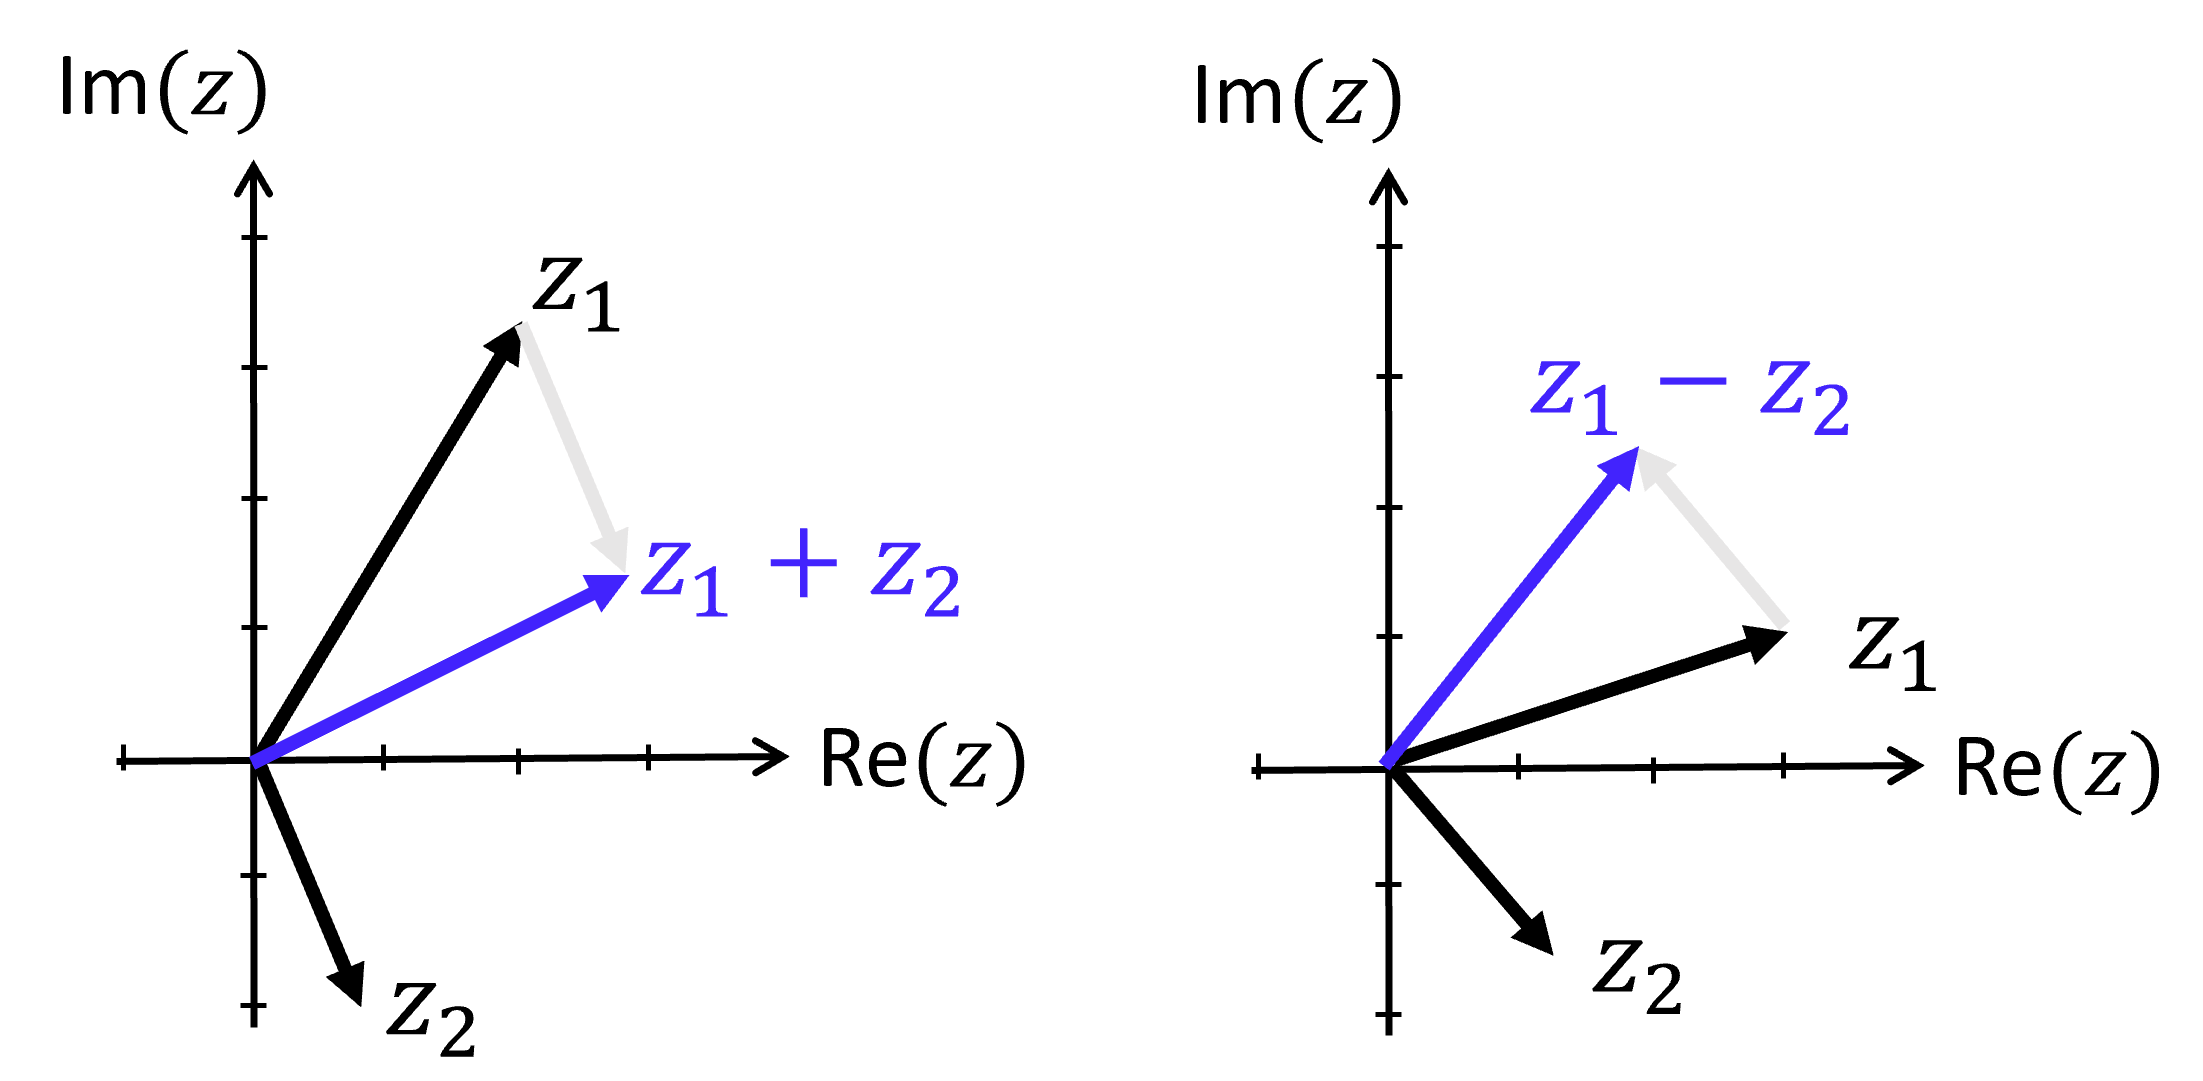
\includegraphics[width=\textwidth]{../Mathematik_1/Bilder/komplexe_zahlen_addition_subtraktion_pfeile.png}
\end{minipage}
\begin{minipage}{0.53\textwidth}

F�r
\[
	z_1=1-2\,i
\qquad\text{und}\qquad
z_2=3+4\,i
\]
gilt
\[
z_1+z_2
=
(1-2\,i)+(3+4\,i)
=
4+2\,i.
\]
Geometrisch werden die beiden zugeh�rigen Pfeile addiert.

F�r die Differenz ergibt sich
\[
z_1-z_2
=
(1-2\,i)-(3+4\,i)
=
-2-6\,i.
\]
Die Subtraktion von \(z_2\) entspricht dabei der Addition des Gegenpfeils
\(-z_2\).

\end{minipage}

\end{exabox}

\subsubsection*{Multiplikation mit \(i\): eine Drehung}

Bei der Addition ist die geometrische Interpretation unmittelbar aus den
kartesischen Koordinaten ablesbar. Bei der Multiplikation ist die Situation
weniger offensichtlich. Einen ersten Zugang liefert die Multiplikation mit
der imagin�ren Einheit \(i\).

F�r
\[
z=a+i\,b
\]
gilt
\[
i\,z
=
i(a+i\,b)
=
i\,a+i^2b
=
-b+i\,a.
\]

Der Punkt
\[
(a\,|\,b)
\]
wird durch die Multiplikation mit \(i\) also auf den Punkt
\[
(-b\,|\,a)
\]
abgebildet. Diese Abbildung entspricht geometrisch einer Drehung um
\[
\frac{\pi}{2}=90^\circ
\]
gegen den Uhrzeigersinn.

\begin{exabox}{Multiplikation mit \(i\): reine Drehung}{ }

\begin{minipage}{0.4\textwidth}
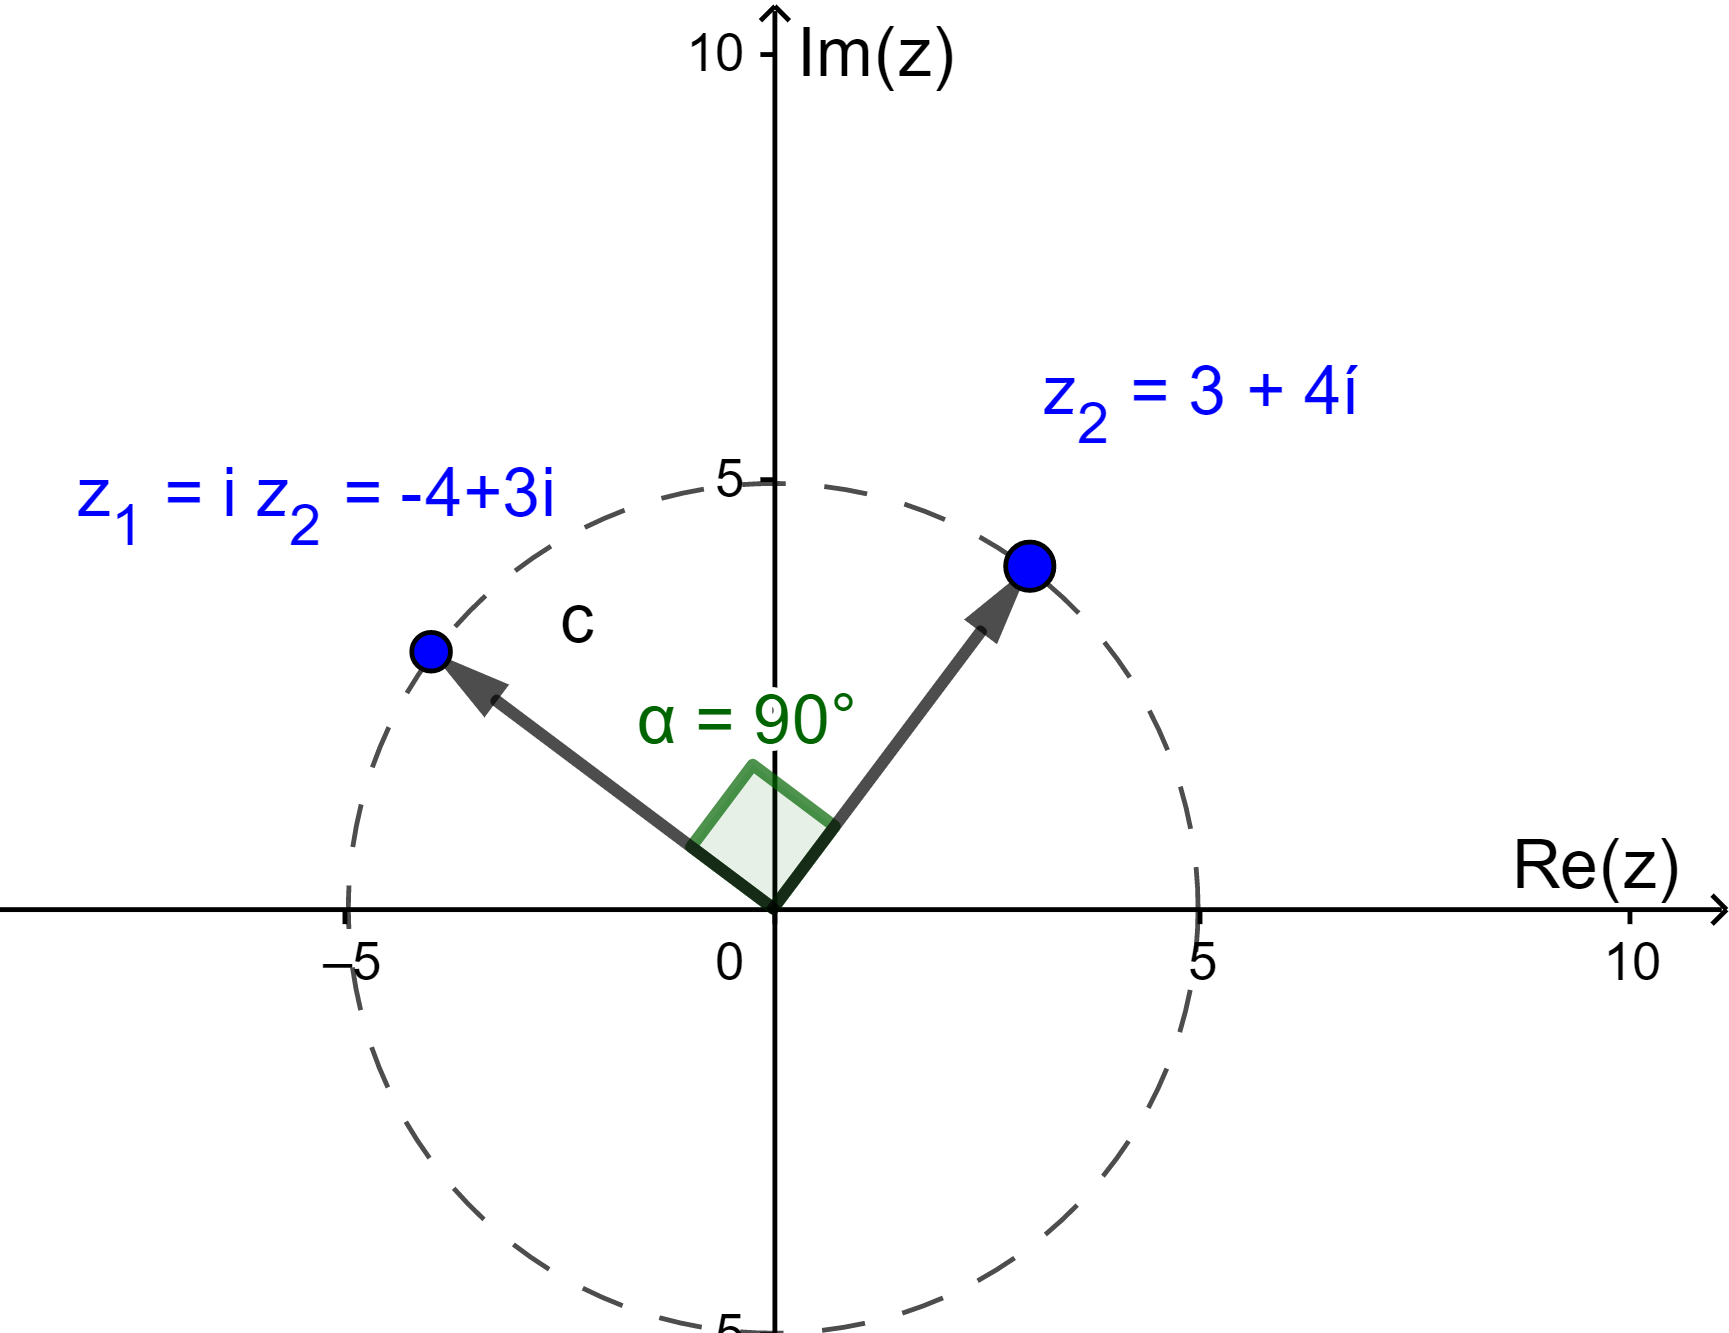
\includegraphics[width=\textwidth]{../Mathematik_1/Bilder/komplexe_zahlen_multiplikation_i_drehung.png}
\end{minipage}
\begin{minipage}{0.58\textwidth}

F�r
\[
z\;\widehat=\;(r\,|\,\varphi)
\]
bleibt bei der Multiplikation mit \(i\) die L�nge des zugeh�rigen Pfeils
unver�ndert:
\[
|i\,z|
=
\sqrt{(-b)^2+a^2}
=
\sqrt{a^2+b^2}
=
|z|
=
r.
\]

Gleichzeitig wird der Pfeil um \(90^\circ\) gegen den Uhrzeigersinn gedreht.
Sein Winkel ver�ndert sich daher von
\[
\varphi
\]
zu
\[
\varphi+\frac{\pi}{2}.
\]

Damit gilt
\[
i\,z
\;\widehat=\;
\left(
r\,\middle|\,\varphi+\frac{\pi}{2}
\right).
\]

\end{minipage}

\end{exabox}

Die Multiplikation mit \(i\) ver�ndert also nicht die L�nge einer komplexen
Zahl, sondern ausschlie�lich ihre Richtung. Sie liefert damit ein erstes
Beispiel daf�r, dass eine Multiplikation in \(\mathbb C\) geometrisch als
Drehung interpretiert werden kann.

\subsubsection*{Multiplikation: Skalierung und Drehung}

Die Multiplikation mit \(i\) zeigt bereits, dass eine Multiplikation in \(\mathbb C\) geometrisch eine Drehung bewirken kann. Bei der Multiplikation mit einer beliebigen komplexen Zahl kommt im Allgemeinen zus�tzlich eine Skalierung hinzu.

Besonders transparent wird dies in Polarkoordinaten. Es seien
\[
z_1\;\widehat=\;(r_1\,|\,\varphi_1)
\qquad\text{und}\qquad
z_2\;\widehat=\;(r_2\,|\,\varphi_2).
\]

Bei der Multiplikation werden die Betr�ge multipliziert und die Winkel
addiert.

\begin{theorembox}{Geometrische Interpretation der Multiplikation}{ }
\begin{minipage}{0.3\textwidth}
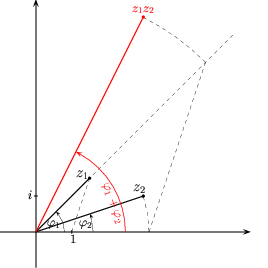
\includegraphics[width=\textwidth]{../Mathematik_1/Bilder/komplexe_zahlen_multiplikation_winkelsumme.png}
\end{minipage}
\begin{minipage}{0.7\textwidth}

F�r
\[
z_1\;\widehat=\;(r_1\,|\,\varphi_1)
\qquad\text{und}\qquad
z_2\;\widehat=\;(r_2\,|\,\varphi_2)
\]
gilt
\[
z_1\cdot z_2
\;\widehat=\;
(r_1\cdot r_2\,|\,\varphi_1+\varphi_2).
\]

Die Multiplikation komplexer Zahlen besitzt damit zwei geometrische
Wirkungen:
\begin{itemize}
    \item Die L�ngen werden multipliziert:
    \[
    |z_1\cdot z_2|=|z_1|\,|z_2|=r_1\cdot r_2.
    \]

    \item Die Winkel werden addiert:
    \[
    \arg(z_1\cdot z_2)
    =
    \varphi_1+\varphi_2
    \qquad \text{bis auf Vielfache von }2\pi.
    \]
\end{itemize}
\end{minipage}

\end{theorembox}

Eine Multiplikation mit einer komplexen Zahl kann somit als Kombination aus
\textbf{Skalierung} und \textbf{Drehung} interpretiert werden. Der Betrag des
Multiplikators bestimmt den Skalierungsfaktor, sein Argument den Drehwinkel.


\subsubsection*{Division: umgekehrte Skalierung und Drehung}

Auch die geometrische Bedeutung der Division l�sst sich aus der
Multiplikation herleiten.

Gesucht sei
\[
z_3=\frac{z_1}{z_2},
\qquad z_2\neq0.
\]
Diese Gleichung ist �quivalent zu
\[
z_2\cdot z_3=z_1.
\]

F�r die Betr�ge gilt daher
\[
r_2\cdot r_3=r_1.
\]
Da \(z_2\neq0\) und damit \(r_2>0\) ist, folgt
\[
r_3=\frac{r_1}{r_2}.
\]

F�r die Winkel gilt entsprechend
\[
\varphi_2+\varphi_3
=
\varphi_1
\qquad
\text{bis auf Vielfache von }2\pi.
\]
Damit ergibt sich
\[
\varphi_3
=
\varphi_1-\varphi_2
\qquad
\text{bis auf Vielfache von }2\pi.
\]

\begin{theorembox}{Geometrische Interpretation der Division}{ }

\begin{minipage}{0.3\textwidth}
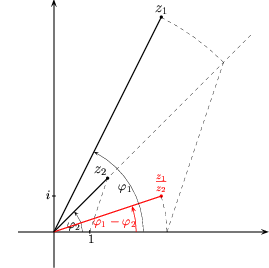
\includegraphics[width=\textwidth]{../Mathematik_1/Bilder/komplexe_zahlen_division_winkeldifferenz.png}
\end{minipage}
\begin{minipage}{0.7\textwidth}

F�r
\[
z_1\;\widehat=\;(r_1\,|\,\varphi_1),
\qquad
z_2\;\widehat=\;(r_2\,|\,\varphi_2),
\qquad
z_2\neq0,
\]
gilt
\[
\frac{z_1}{z_2}
\;\widehat=\;
\left(
\frac{r_1}{r_2}
\,\middle|\,
\varphi_1-\varphi_2
\right).
\]

Bei der Division werden somit die L�ngen dividiert und die Winkel
subtrahiert.
\end{minipage}

\end{theorembox}

\noindent\textbf{Bemerkung:}
Winkel sind nur bis auf ganzzahlige Vielfache von \(2\pi\) eindeutig
bestimmt. Bei der Addition oder Subtraktion von Argumenten kann daher ein
Winkel entstehen, der au�erhalb des gew�hlten Hauptintervalls
\[
(-\pi,\pi]
\]
liegt. Durch Addition oder Subtraktion eines geeigneten ganzzahligen
Vielfachen von \(2\pi\) kann wieder der entsprechende Hauptwert bestimmt
werden.

\medskip

Die geometrische Interpretation der Grundrechenarten l�sst sich damit
besonders kompakt zusammenfassen:
\[
\begin{array}{ccl}
\text{Addition}
&\longleftrightarrow&
\text{Pfeiladdition},\\[1mm]
\text{Multiplikation}
&\longleftrightarrow&
\text{L�ngen multiplizieren und Winkel addieren},\\[1mm]
\text{Division}
&\longleftrightarrow&
\text{L�ngen dividieren und Winkel subtrahieren}.
\end{array}
\]

Insbesondere die Multiplikation zeigt, warum die Polardarstellung f�r
komplexe Zahlen so n�tzlich ist. In kartesischer Darstellung ist eine
Multiplikation vergleichsweise aufwendig; in Polarkoordinaten werden
lediglich Betr�ge multipliziert und Winkel addiert.

Diese Beobachtung bildet den Ausgangspunkt f�r die n�chste Darstellung
komplexer Zahlen. Die Beziehung
\[
z
=
r\bigl(\cos(\varphi)+i\sin(\varphi)\bigr)
\]
wird dort mithilfe der komplexen Exponentialfunktion in eine noch kompaktere
Form �berf�hrt.

  %  Kartesische und Polarkoordinaten, geometrische Interpretation der Grundrechenarten
\newpage
\setcounter{satz}{0} \setcounter{def}{0} \setcounter{exa}{0}  
\section{Komplexe Zahlen II: Polarform, Euler und Schwingungen}\label{MA1-komplexe-zahlen-polarform-und-euler}

\begin{table}[H]
  \centering
  \begin{tabularx}{\textwidth}{p{0.9\textwidth} p{0.1\textwidth}}
    \toprule
    \multicolumn{2}{c}{\textbf{�bersicht �ber Lernziele und Voraussetzungen}}\\
    \midrule
    \textbf{Lernziele} &\\[.5\normalbaselineskip]
    \tabitem die Polarform komplexer Zahlen zum Potenzieren und Wurzelziehen nutzen &\\
    \tabitem alle L�sungen einer Gleichung der Form \(z^n=c\) bestimmen und geometrisch interpretieren &\\
    \tabitem die Eulersche Formel erkl�ren und komplexe Zahlen in Exponentialdarstellung schreiben &\\
    \tabitem die komplexe Exponentialfunktion geometrisch interpretieren &\\
    \tabitem harmonische Schwingungen mithilfe komplexer Amplituden (Phasoren) darstellen &\\
    \tabitem harmonische Schwingungen gleicher Frequenz mithilfe komplexer Amplituden �berlagern &\\
    \tabitem Polynome �ber \(\mathbb C\) vollst�ndig in Linearfaktoren zerlegen &\\[.5\normalbaselineskip]
    \midrule
    \textbf{Voraussetzungen} &\\[.5\normalbaselineskip]
    \tabitem Betrag, Argument und Polarform komplexer Zahlen & \abschnittsverweis{MA1-komplexe-zahlen-grundlagen}\\
    \tabitem Multiplikation und Division komplexer Zahlen in geometrischer Darstellung & \abschnittsverweis{MA1-komplexe-zahlen-grundlagen}\\
    \tabitem Potenzen und Wurzeln reeller Zahlen & \abschnittsverweis{MA1-potenz-und-wurzelfunktionen}\\
    \tabitem Exponentialfunktion & \abschnittsverweis{MA1-exponential-und-logarithmusfunktionen}\\
    \tabitem trigonometrische Funktionen und harmonische Schwingungen & \abschnittsverweis{MA1-trigonometrische-funktionen}\\
    \bottomrule
  \end{tabularx}
\end{table}

\ifintegriereaufgaben
\noindent �bungsaufgaben zu diesem Abschnitt:
\hyperref[MA1-komplexe-zahlen-polarform-und-euler-aufgaben]{Aufgaben}
\vspace{0.3cm}
\hrule
\fi


% --------------------------------------------------------------------------
\subsection{Potenzen und Wurzeln in Polarform}

Im vorangegangenen Abschnitt wurden komplexe Zahlen sowohl in kartesischer
Form \(z=a+i\,b\) als auch mithilfe von Betrag und Winkel dargestellt. F�r
\(z\neq0\) gilt
\[
z=r\bigl(\cos(\varphi)+i\sin(\varphi)\bigr),
\qquad
r=|z|,
\qquad
\varphi=\arg(z).
\]

Dabei zeigte sich bereits ein wesentlicher Vorteil der Polardarstellung. F�r
zwei komplexe Zahlen
\[
z_1\;\widehat=\;(r_1\,|\,\varphi_1),
\qquad
z_2\;\widehat=\;(r_2\,|\,\varphi_2)
\]
gilt
\[
z_1z_2
\;\widehat=\;
(r_1r_2\,|\,\varphi_1+\varphi_2).
\]
Bei einer Multiplikation werden also die Betr�ge multipliziert und die Winkel
addiert.

Diese geometrische Interpretation f�hrt unmittelbar zu zwei weiteren Fragen:
Was geschieht, wenn eine komplexe Zahl mehrfach mit sich selbst multipliziert
wird? Und wie lassen sich umgekehrt alle komplexen Zahlen bestimmen, deren
\(n\)-te Potenz eine vorgegebene komplexe Zahl ergibt?

Damit f�hren Multiplikation und Polardarstellung auf nat�rliche Weise zum
\textbf{Potenzieren} und zum \textbf{Wurzelziehen} in \(\mathbb C\).


% --------------------------------------------------------------------------
\subsubsection*{Positive ganzzahlige Potenzen}

Wird eine komplexe Zahl \(z\;\widehat=\;(r\,|\,\varphi)\) mit sich selbst
multipliziert, ergibt sich
\[
z^2=z\cdot z
\;\widehat=\;
(r^2\,|\,2\varphi).
\]
Eine weitere Multiplikation mit \(z\) liefert
\(z^3\;\widehat=\;(r^3\,|\,3\varphi)\). Dieses Muster setzt sich f�r jede
positive ganzzahlige Potenz fort.

\begin{theorembox}{Potenzieren in Polarkoordinaten}{ }

F�r \(z\;\widehat=\;(r\,|\,\varphi)\) und \(n\in\mathbb N^+\) gilt
\[
z^n
\;\widehat=\;
(r^n\,|\,n\varphi).
\]

Beim Potenzieren wird der Betrag zur \(n\)-ten Potenz erhoben, w�hrend der
Winkel mit \(n\) multipliziert wird.

\end{theorembox}

\begin{exabox}{Potenzen einer komplexen Zahl}{ }

Betrachtet wird die komplexe Zahl
\[
z
\;\widehat=\;
\left(
\sqrt2\,\middle|\,\frac{\pi}{4}
\right).
\]

F�r die zweite Potenz ergibt sich
\[
\begin{aligned}
z^2
&\;\widehat=\;
\left(
(\sqrt2)^2
\,\middle|\,
2\frac{\pi}{4}
\right)\\
&=
\left(
2\,\middle|\,\frac{\pi}{2}
\right).
\end{aligned}
\]

F�r die dritte Potenz folgt entsprechend
\[
\begin{aligned}
z^3
&\;\widehat=\;
\left(
(\sqrt2)^3
\,\middle|\,
3\frac{\pi}{4}
\right)\\
&=
\left(
2\sqrt2
\,\middle|\,
\frac{3\pi}{4}
\right).
\end{aligned}
\]

Das Beispiel macht beide Wirkungen des Potenzierens sichtbar: Der Betrag
ver�ndert sich durch die Potenz \(r^n\), w�hrend sich der Winkel mit jeder
weiteren Multiplikation um \(\varphi\) vergr��ert.

\end{exabox}

Die geometrischen Wirkung des Potenzierens l�sst sich interaktiv untersuchen, beispielsweise in der GeoGebra Anwendung
\href{https://www.geogebra.org/m/jsda7yjz}{Potenzieren komplexer Zahlen}.

\subsubsection*{Negative ganzzahlige Potenzen}

F�r \(z\neq0\) sind auch negative ganzzahlige Potenzen definiert. Dabei gilt
beispielsweise \(z^{-1}=1/z\). Die Division komplexer Zahlen wurde im
vorangegangenen Abschnitt bereits geometrisch als Division der Betr�ge und
Subtraktion der Winkel interpretiert.

F�r \(z\;\widehat=\;(r\,|\,\varphi)\) folgt daher
\[
z^{-1}
\;\widehat=\;
\left(
\frac{1}{r}\,\middle|\,-\varphi
\right).
\]

Allgemeiner gilt f�r \(n\in\mathbb N^+\)
\[
z^{-n}
\;\widehat=\;
(r^{-n}\,|\,-n\varphi).
\]

\begin{exabox}{Negative Potenzen}{ }

F�r
\[
z
\;\widehat=\;
\left(
\sqrt2\,\middle|\,\frac{\pi}{4}
\right)
\]
gilt zun�chst
\[
z^0=1
\;\widehat=\;
(1\,|\,0).
\]

F�r den Kehrwert ergibt sich
\[
z^{-1}
\;\widehat=\;
\left(
\frac{1}{\sqrt2}
\,\middle|\,
-\frac{\pi}{4}
\right).
\]

Der Betrag wird beim Bilden des Kehrwerts also invertiert, w�hrend sich das
Vorzeichen des Winkels �ndert.

\end{exabox}

Positive, negative und die nullte Potenz lassen sich damit gemeinsam
beschreiben: F�r \(z\neq0\) und \(n\in\mathbb Z\) gilt
\[
z^n
\;\widehat=\;
(r^n\,|\,n\varphi).
\]


\subsubsection*{Die Umkehrfrage: Wurzeln komplexer Zahlen}

Das Potenzieren f�hrt unmittelbar auf die Umkehrfrage. Gesucht seien
beispielsweise alle komplexen Zahlen \(z\), f�r die
\[
z^3=8i
\]
gilt.

Die rechte Seite besitzt den Betrag \(8\) und den Winkel \(\pi/2\), also
\[
8i
\;\widehat=\;
\left(
8\,\middle|\,\frac{\pi}{2}
\right).
\]

F�r die gesuchte Zahl wird
\(z\;\widehat=\;(r\,|\,\varphi)\) angesetzt. Dann gilt
\[
z^3
\;\widehat=\;
(r^3\,|\,3\varphi).
\]

Ein erster Vergleich von Betrag und Winkel liefert
\[
r^3=8
\qquad\text{und}\qquad
3\varphi=\frac{\pi}{2}.
\]
Damit ergibt sich \(r=2\) und \(\varphi=\pi/6\). Eine L�sung lautet also
\[
z_0
\;\widehat=\;
\left(
2\,\middle|\,\frac{\pi}{6}
\right).
\]

Damit ist die Gleichung jedoch noch nicht vollst�ndig gel�st. Der Winkel
\(\pi/2\) beschreibt dieselbe Richtung wie jeder Winkel
\[
\frac{\pi}{2}+2\pi k,
\qquad k\in\mathbb Z.
\]
F�r die gesuchten Winkel muss daher allgemeiner
\[
3\varphi_k
=
\frac{\pi}{2}+2\pi k
\]
gelten. Somit folgt
\[
\varphi_k
=
\frac13
\left(
\frac{\pi}{2}+2\pi k
\right).
\]

F�r \(k=0,1,2\) entstehen drei verschiedene komplexe Zahlen.

\begin{exabox}{Die drei L�sungen von \(z^3=8i\)}{ }

\begin{minipage}{0.4\textwidth}
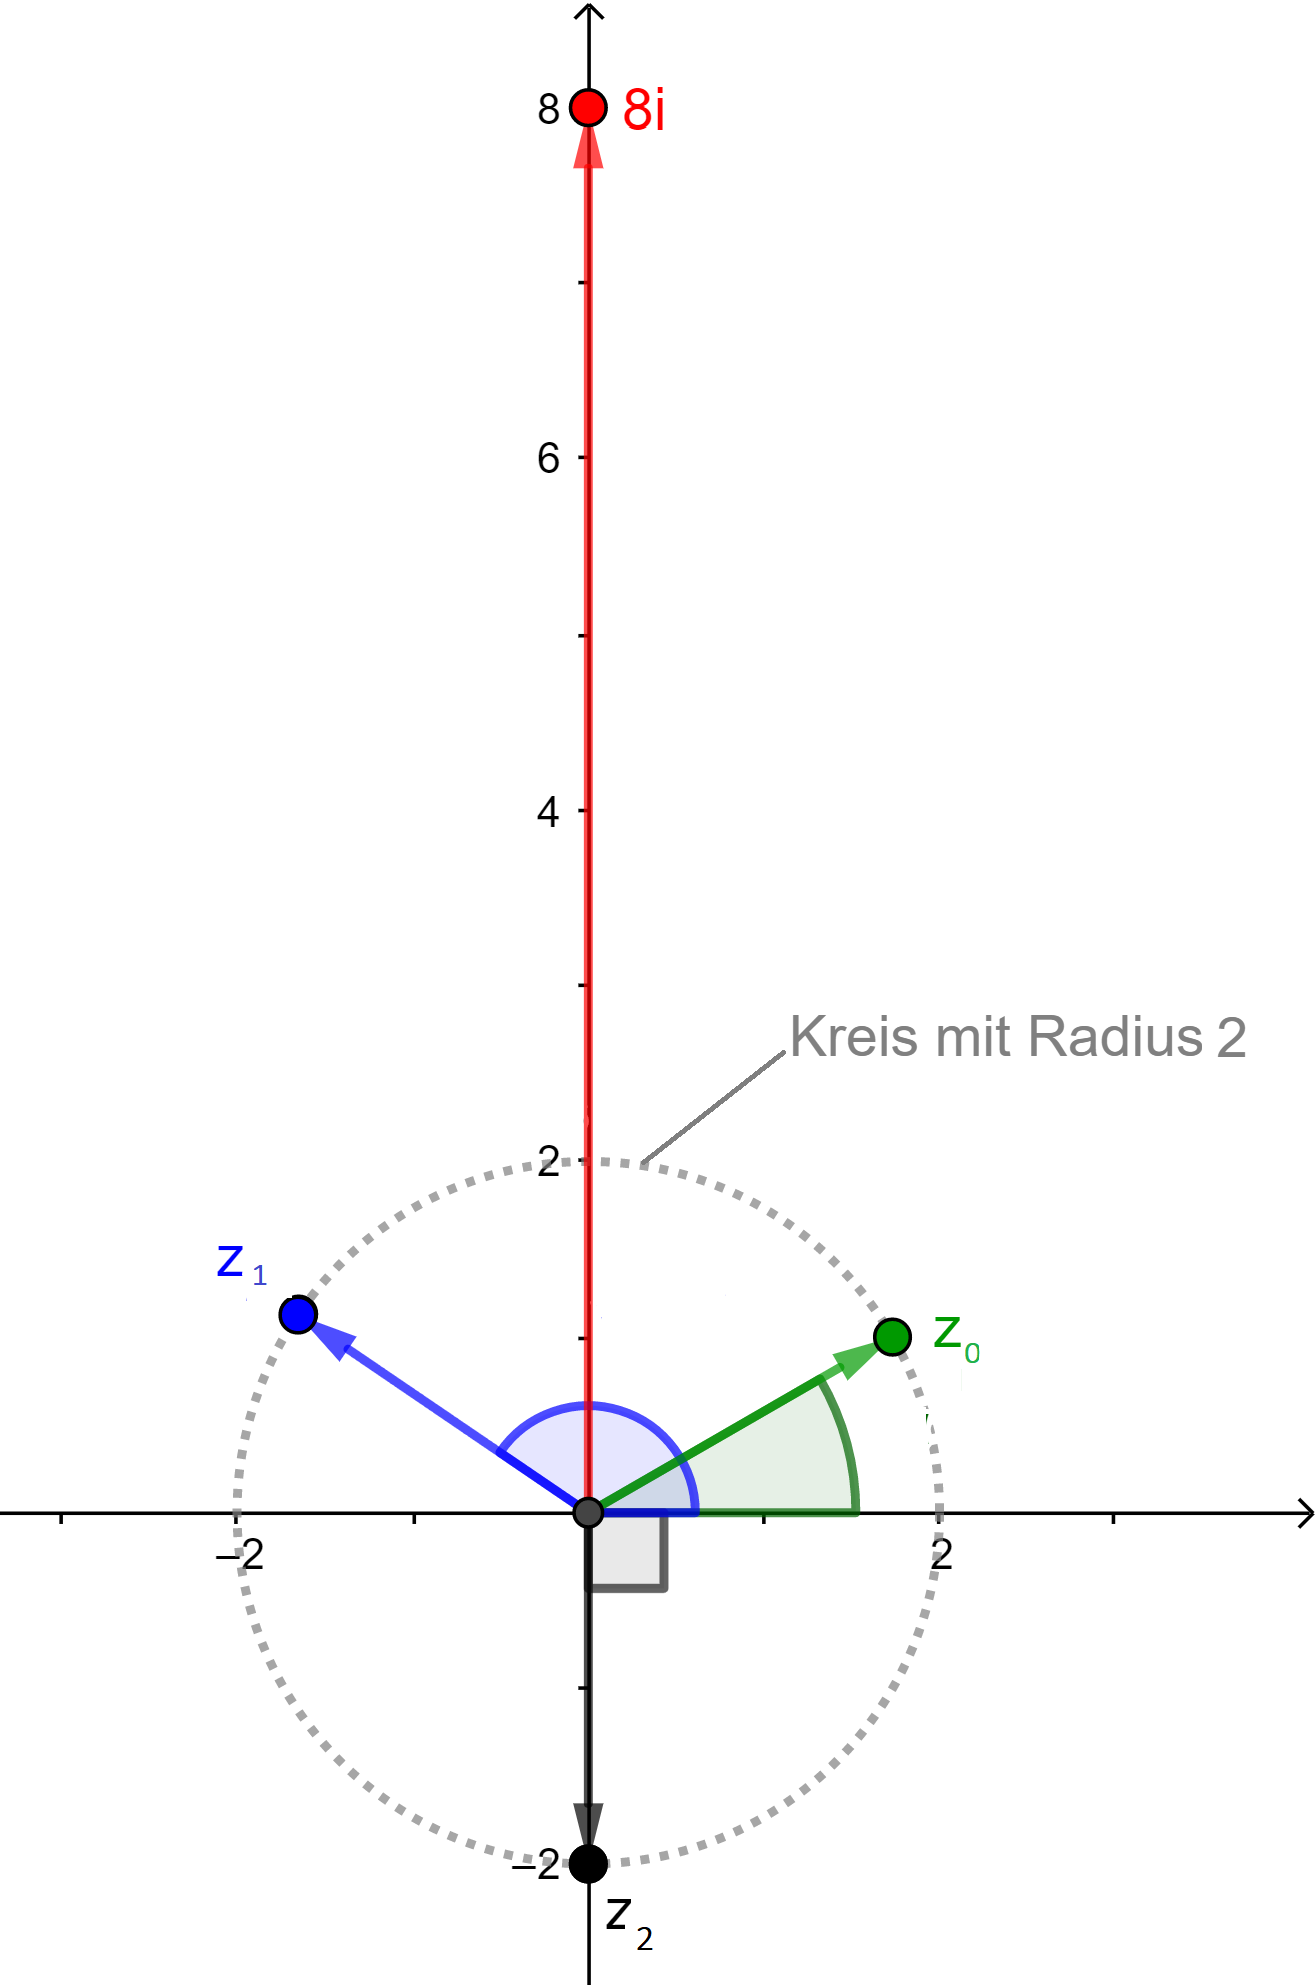
\includegraphics[width=\textwidth]{../Mathematik_1/Bilder/komplexe_zahlen_dritte_wurzeln_acht_i.png}
\end{minipage}
\begin{minipage}{0.58\textwidth}

F�r \(k=0\) gilt
\[
\varphi_0
=
\frac13\frac{\pi}{2}
=
\frac{\pi}{6},
\]
also
\[
z_0
\;\widehat=\;
\left(
2\,\middle|\,\frac{\pi}{6}
\right).
\]

F�r \(k=1\) ergibt sich
\[
\varphi_1
=
\frac13
\left(
\frac{\pi}{2}+2\pi
\right)
=
\frac{5\pi}{6},
\]
also
\[
z_1
\;\widehat=\;
\left(
2\,\middle|\,\frac{5\pi}{6}
\right).
\]

F�r \(k=2\) folgt zun�chst
\[
\varphi_2
=
\frac13
\left(
\frac{\pi}{2}+4\pi
\right)
=
\frac{3\pi}{2}.
\]
Da \(\frac{3\pi}{2}\) und \(-\frac{\pi}{2}\) dieselbe Richtung beschreiben,
kann die dritte L�sung im gew�hlten Hauptintervall als
\[
z_2
\;\widehat=\;
\left(
2\,\middle|\,-\frac{\pi}{2}
\right)
\]
geschrieben werden.

\end{minipage}

\end{exabox}

Alle drei L�sungen besitzen denselben Betrag \(2\). Sie liegen daher auf
einem Kreis mit Radius \(2\) um den Ursprung. Gleichzeitig unterscheiden
sich ihre Winkel jeweils um \(2\pi/3\). Die L�sungen sind also gleichm��ig
auf diesem Kreis verteilt.

Das Beispiel zeigt, warum das Wurzelziehen in \(\mathbb C\) anders behandelt
werden muss als in \(\mathbb R\): Die Mehrdeutigkeit der Winkel f�hrt dazu,
dass eine Gleichung der Form \(z^n=c\) im Allgemeinen mehrere verschiedene
komplexe L�sungen besitzt.


\subsubsection*{Allgemeine \(n\)-te Wurzeln}

Das Vorgehen aus dem vorangegangenen Beispiel l�sst sich auf eine beliebige
komplexe Zahl �bertragen. Gesucht seien alle L�sungen von
\[
z^n=c,
\qquad
c\in\mathbb C\setminus\{0\}.
\]

Die rechte Seite werde durch
\[
c
\;\widehat=\;
(\rho\,|\,\psi),
\qquad
\rho=|c|>0,
\]
beschrieben. F�r die gesuchte Zahl wird
\(z\;\widehat=\;(r\,|\,\varphi)\) angesetzt. Dann gilt
\[
z^n
\;\widehat=\;
(r^n\,|\,n\varphi).
\]

Da neben \(\psi\) auch alle Winkel \(\psi+2\pi k\) dieselbe komplexe Zahl
\(c\) beschreiben, m�ssen die Bedingungen
\[
r^n=\rho
\qquad\text{und}\qquad
n\varphi=\psi+2\pi k
\]
erf�llt sein.

Daraus folgen
\[
r=\sqrt[n]{\rho}
\qquad\text{und}\qquad
\varphi_k=\frac{\psi+2\pi k}{n}.
\]

\begin{theorembox}{\(n\)-te Wurzeln einer komplexen Zahl}{ }

F�r
\[
c
=
\rho\bigl(\cos(\psi)+i\sin(\psi)\bigr)
\neq0
\]
besitzt die Gleichung \(z^n=c\) genau \(n\) verschiedene L�sungen
\[
z_k
=
\sqrt[n]{\rho}
\left(
\cos\left(\frac{\psi+2\pi k}{n}\right)
+
i\sin\left(\frac{\psi+2\pi k}{n}\right)
\right),
\]
wobei
\[
k=0,1,\ldots,n-1.
\]

Alle \(n\) L�sungen besitzen denselben Betrag \(\sqrt[n]{\rho}\) und liegen
daher auf einem Kreis um den Ursprung. Die Winkel zweier aufeinanderfolgender
L�sungen unterscheiden sich um \(2\pi/n\). Die \(n\) Wurzeln sind somit
gleichm��ig auf diesem Kreis verteilt.

\end{theorembox}

Die \(n\) verschiedenen L�sungen entstehen also nicht durch verschiedene
Betr�ge, sondern durch die verschiedenen Winkel, die sich aus der
Mehrdeutigkeit des Arguments ergeben.

\noindent\textbf{Bemerkung:}
Das Symbol \(\sqrt[n]{c}\) ist bei komplexen Zahlen mit Vorsicht zu
interpretieren. W�hrend eine Gleichung wie \(z^n=c\) alle \(n\) L�sungen
beschreibt, bezeichnet ein Wurzelsymbol je nach Konvention h�ufig nur einen
ausgew�hlten Hauptwert. Bei der L�sung komplexer Gleichungen ist die
Formulierung \(z^n=c\) daher h�ufig eindeutiger.


\subsection{Von der Polarform zur komplexen Exponentialfunktion}

Die Polardarstellung hat gezeigt, dass die Multiplikation komplexer Zahlen
eine besonders einfache Wirkung auf ihre geometrischen Gr��en besitzt:
Betr�ge werden multipliziert und Winkel addiert.

Damit erinnert das Verhalten der Winkel an eine bereits bekannte Eigenschaft
der Exponential- beziehungsweise Logarithmusrechnung. Auch dort wird eine
Addition im Exponenten bei der Exponentialfunktion zu einer Multiplikation:
\[
e^{x+y}=e^x e^y.
\]

Es liegt daher nahe, nach einer Darstellung zu suchen, in der auch die
Addition von Winkeln durch die bekannten Potenzgesetze beschrieben werden
kann. Genau diese Verbindung wird durch die komplexe Exponentialfunktion
hergestellt.


\subsubsection*{Motivation auf dem Einheitskreis}

Auf dem Einheitskreis besitzt jede komplexe Zahl den Betrag \(1\) und ist
damit vollst�ndig durch ihren Winkel bestimmt. F�r einen Winkel \(\alpha\)
gilt
\[
c
=
\cos(\alpha)+i\sin(\alpha).
\]

Die folgende �berlegung motiviert, warum an dieser Stelle gerade die
Exponentialfunktion auftritt. Sie dient als anschaulicher Zugang und ersetzt
keinen vollst�ndigen analytischen Beweis.

Wird der Winkel \(\alpha\) in \(n\) kleine gleich gro�e Winkel zerlegt, so
besitzt die zugeh�rige komplexe Zahl
\[
z
\;\widehat=\;
\left(
1\,\middle|\,\frac{\alpha}{n}
\right)
\]
die Eigenschaft \(z^n=c\).

F�r gro�e \(n\) ist der Winkel \(\alpha/n\) klein. Auf dem Einheitskreis liegt
der zugeh�rige Punkt dann nahe bei \(1\). F�r kleine Winkel gilt n�herungsweise
\[
\cos\left(\frac{\alpha}{n}\right)\approx1
\qquad\text{und}\qquad
\sin\left(\frac{\alpha}{n}\right)\approx\frac{\alpha}{n}.
\]
Damit ergibt sich
\[
z
=
\cos\left(\frac{\alpha}{n}\right)
+
i\sin\left(\frac{\alpha}{n}\right)
\approx
1+i\frac{\alpha}{n}.
\]

Da \(c=z^n\) gilt, folgt n�herungsweise
\[
c
\approx
\left(
1+i\frac{\alpha}{n}
\right)^n.
\]

Dieser Ausdruck erinnert an die bekannte Grenzwertdarstellung der
Exponentialfunktion
\[
e^x
=
\lim_{n\to\infty}
\left(
1+\frac{x}{n}
\right)^n.
\]
Wird diese Struktur auf das komplexe Argument \(x=i\alpha\) erweitert, f�hrt
sie auf die Verbindung zwischen Exponentialfunktion und Einheitskreis.


\subsubsection*{Eulersche Formel}

\begin{theorembox}{Eulersche Formel}{ }

F�r jeden reellen Winkel \(\varphi\) gilt
\[
e^{i\varphi}
=
\cos(\varphi)+i\sin(\varphi).
\]

\end{theorembox}

Die Eulersche Formel verbindet drei zuvor getrennt betrachtete mathematische
Objekte: die Exponentialfunktion, die trigonometrischen Funktionen und die
Geometrie des Einheitskreises.

Da
\[
|e^{i\varphi}|=1,
\]
liegt \(e^{i\varphi}\) f�r jedes \(\varphi\in\mathbb R\) auf dem
Einheitskreis. Sein Argument ist \(\varphi\) bis auf ganzzahlige Vielfache
von \(2\pi\).

F�r den besonderen Winkel \(\varphi=\pi\) gilt
\[
e^{i\pi}
=
\cos(\pi)+i\sin(\pi)
=
-1.
\]
Damit folgt
\[
e^{i\pi}+1=0.
\]
Diese besondere Beziehung wird als \textbf{Eulersche Identit�t}
(\emph{Euler's identity}) bezeichnet.


\subsubsection*{Exponentialdarstellung komplexer Zahlen}

Eine beliebige komplexe Zahl \(z\neq0\) besitzt in Polardarstellung die Form
\[
z
=
r\bigl(\cos(\varphi)+i\sin(\varphi)\bigr).
\]
Mit der Eulerschen Formel kann der Ausdruck in der Klammer durch
\(e^{i\varphi}\) ersetzt werden. Damit ergibt sich
\[
z=r\,e^{i\varphi}.
\]

\begin{theorembox}{Exponentialdarstellung komplexer Zahlen}{ }

F�r jede komplexe Zahl \(z\neq0\) gilt
\[
z=r\,e^{i\varphi},
\]
wobei \(r=|z|>0\) und \(\varphi\) ein Argument von \(z\) ist.

Die Winkel \(\varphi+2\pi k\) mit \(k\in\mathbb Z\) beschreiben dieselbe
komplexe Zahl, denn
\[
e^{i(\varphi+2\pi k)}
=
e^{i\varphi}.
\]

\end{theorembox}

Die Exponentialdarstellung ist damit keine neue geometrische Darstellung, sondern eine besonders kompakte Schreibweise der bereits bekannten Polardarstellung.

Ihr Vorteil zeigt sich unmittelbar beim Rechnen. F�r \(z_1=r_1e^{i\varphi_1}\) und \(z_2=r_2e^{i\varphi_2}\) gilt
\[
z_1z_2
=
r_1r_2e^{i(\varphi_1+\varphi_2)}
\]
und f�r \(z_2\neq0\)
\[
\frac{z_1}{z_2}
=
\frac{r_1}{r_2}
e^{i(\varphi_1-\varphi_2)}.
\]

Auch die zuvor geometrisch entwickelte Potenzregel erh�lt nun eine besonders kurze algebraische Form:
\[
\left(re^{i\varphi}\right)^n
=
r^n e^{in\varphi}.
\]

Die Exponentialdarstellung liefert damit dieselben Regeln, die zuvor aus der Geometrie der komplexen Zahlen gewonnen wurden. Sie fasst diese Regeln jedoch in der bekannten Algebra der Exponentialfunktion zusammen.


\subsubsection*{Sinus und Kosinus mithilfe der Exponentialfunktion}

Die Eulersche Formel kann auch verwendet werden, um Sinus und Kosinus durch komplexe Exponentialfunktionen darzustellen. Neben
\[
e^{i\varphi}
=
\cos(\varphi)+i\sin(\varphi)
\]
gilt wegen der Symmetrieeigenschaften von Sinus und Kosinus
\[
e^{-i\varphi}
=
\cos(\varphi)-i\sin(\varphi).
\]

Durch Addition beider Gleichungen folgt
\[
e^{i\varphi}+e^{-i\varphi}
=
2\cos(\varphi),
\]
also
\[
\cos(\varphi)
=
\frac12
\left(
e^{i\varphi}+e^{-i\varphi}
\right).
\]

Durch Subtraktion ergibt sich
\[
e^{i\varphi}-e^{-i\varphi}
=
2i\sin(\varphi)
\]
und damit
\[
\sin(\varphi)
=
\frac{1}{2i}
\left(
e^{i\varphi}-e^{-i\varphi}
\right).
\]

Diese Darstellungen spielen insbesondere bei der Untersuchung von
Schwingungen eine wichtige Rolle.

\subsection{Die komplexe Exponentialfunktion}

Die Eulersche Formel beschreibt zun�chst die Exponentialfunktion f�r rein
imagin�re Zahlen. Sie erm�glicht zugleich, die Exponentialfunktion auf
beliebige komplexe Zahlen zu erweitern.

F�r
\[
z=a+i\,b,
\qquad
a,b\in\mathbb R,
\]
gilt
\[
e^z
=
e^{a+ib}
=
e^a e^{ib}.
\]
Mit der Eulerschen Formel folgt
\[
e^z
=
e^a\bigl(\cos(b)+i\sin(b)\bigr).
\]

\begin{defbox}{Komplexe Exponentialfunktion}{ }

Die \textbf{komplexe Exponentialfunktion}
(\emph{complex exponential function}) ist die Abbildung
\[
\exp:\mathbb C\to\mathbb C,
\qquad
z\mapsto e^z,
\]
mit
\[
e^{a+ib}
=
e^a\bigl(\cos(b)+i\sin(b)\bigr).
\]

\end{defbox}

Diese Darstellung zeigt, dass Real- und Imagin�rteil des Exponenten
unterschiedliche geometrische Wirkungen besitzen. F�r \(z=a+i\,b\) bestimmt
der Realteil \(a\) �ber den Faktor \(e^a\) den Betrag, w�hrend der
Imagin�rteil \(b\) den Winkel bestimmt.

Insbesondere gilt
\[
|e^{a+ib}|=e^a.
\]
Eine Ver�nderung des Realteils ver�ndert somit den Betrag, w�hrend eine
Ver�nderung des Imagin�rteils eine Drehung in der komplexen Ebene bewirkt.


% --------------------------------------------------------------------------
\subsubsection*{Komplexe Exponentialfunktionen einer reellen Variablen}

F�r die Beschreibung zeitabh�ngiger Vorg�nge wird nun die komplexe
Exponentialfunktion mit einer reellen Variablen \(t\) verbunden. Dazu sei
\[
\lambda=\sigma+i\omega
\]
eine feste komplexe Zahl. Betrachtet wird die Funktion
\[
f:\mathbb R\to\mathbb C,
\qquad
t\mapsto e^{\lambda t}.
\]

Da
\[
\lambda t
=
(\sigma+i\omega)t
=
\sigma t+i\omega t,
\]
ergibt sich
\[
\begin{aligned}
e^{\lambda t}
&=
e^{(\sigma+i\omega)t}\\
&=
e^{\sigma t}e^{i\omega t}\\
&=
e^{\sigma t}
\bigl(\cos(\omega t)+i\sin(\omega t)\bigr).
\end{aligned}
\]

Diese Darstellung verbindet zwei geometrisch unterschiedliche Vorg�nge.
Der Faktor \(e^{\sigma t}\) bestimmt die L�nge des zugeh�rigen Zeigers,
w�hrend \(e^{i\omega t}\) seine Drehung beschreibt.

F�r den Betrag gilt
\[
|e^{\lambda t}|=e^{\sigma t}.
\]
Damit h�ngt die zeitliche Entwicklung der Zeigerl�nge vom Vorzeichen von
\(\sigma\) ab. F�r \(\sigma<0\) nimmt der Betrag exponentiell ab, f�r
\(\sigma>0\) w�chst er exponentiell. Im Fall \(\sigma=0\) bleibt der Betrag
konstant.

Der Winkel ver�ndert sich gleichzeitig mit \(\omega t\). Der Parameter
\(\omega\) bestimmt damit die Winkelgeschwindigkeit der Drehung.

Die Funktion
\[
t\mapsto e^{(\sigma+i\omega)t}
\]
verbindet somit exponentielles Wachstum beziehungsweise exponentielle
D�mpfung mit einer gleichf�rmigen Drehung in der komplexen Ebene.


% --------------------------------------------------------------------------
\subsubsection*{Der Spezialfall \(e^{i\omega t}\): rotierender Zeiger}

F�r \(\sigma=0\) vereinfacht sich die komplexe Exponentialfunktion zu
\[
e^{i\omega t}
=
\cos(\omega t)+i\sin(\omega t).
\]

Da
\[
|e^{i\omega t}|=1,
\]
bleibt die L�nge des zugeh�rigen Zeigers konstant. Mit wachsendem \(t\)
ver�ndert sich ausschlie�lich sein Winkel. Die Spitze des Zeigers bewegt
sich daher auf dem Einheitskreis.

\begin{exabox}{Rotierender Zeiger und harmonische Schwingung}{ }

\begin{minipage}{0.4\textwidth}
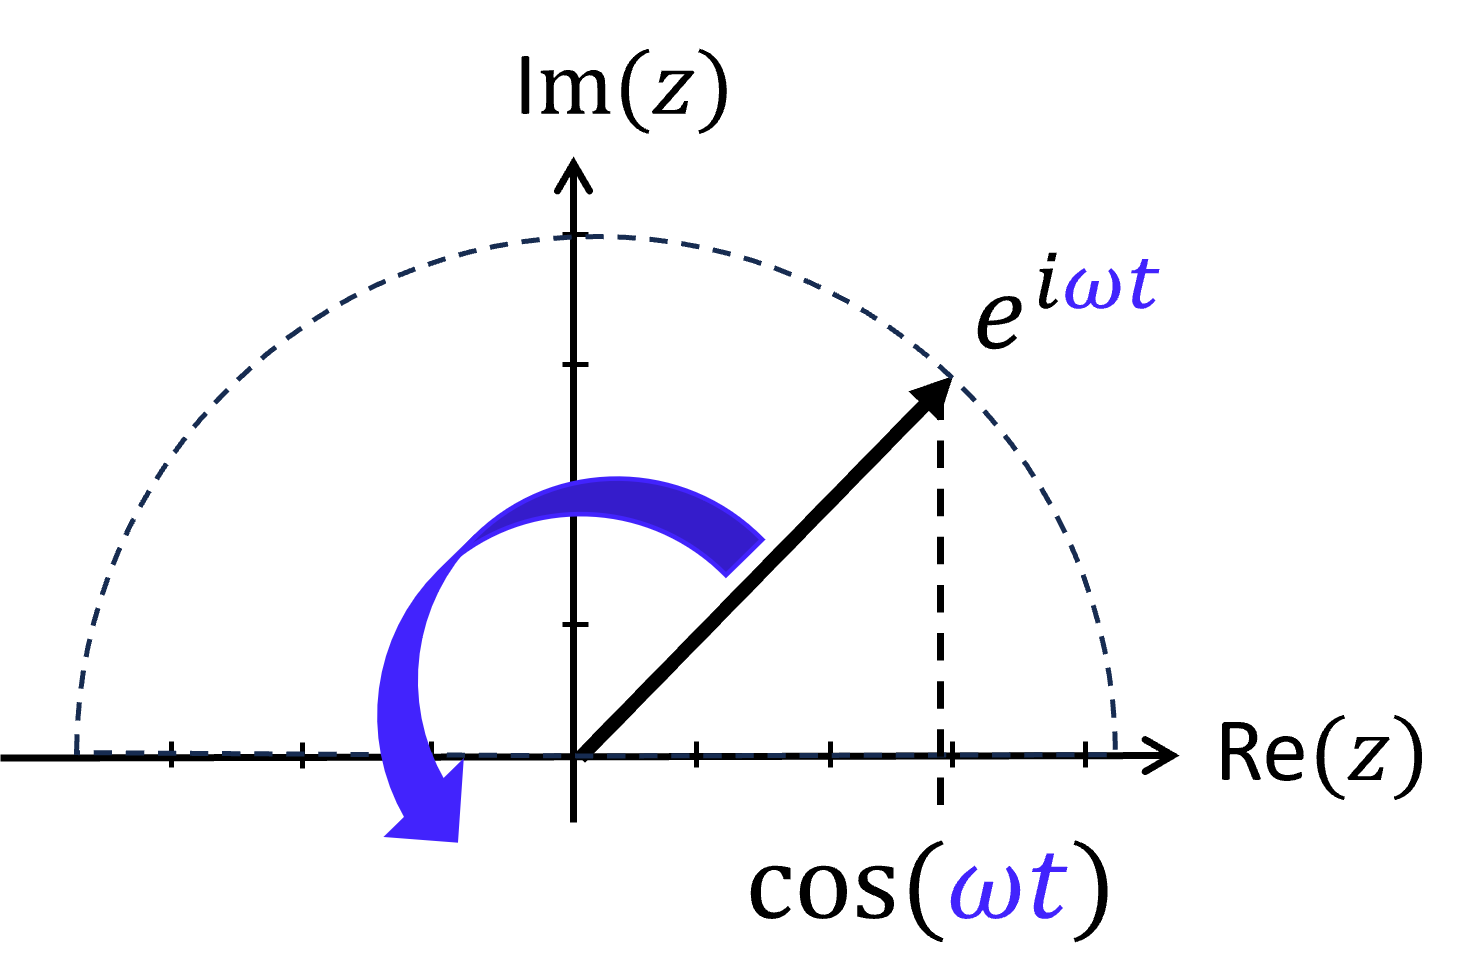
\includegraphics[width=\textwidth]{../Mathematik_1/Bilder/komplexe_zahlen_rotierender_zeiger.png}
\end{minipage}
\begin{minipage}{0.58\textwidth}

Der komplexe Ausdruck
\[
e^{i\omega t}
\]
beschreibt einen Zeiger, der sich mit der Winkelgeschwindigkeit \(\omega\)
auf dem Einheitskreis dreht.

Sein Realteil ist
\[
\mathrm{Re}\left(e^{i\omega t}\right)
=
\cos(\omega t),
\]
sein Imagin�rteil ist
\[
\mathrm{Im}\left(e^{i\omega t}\right)
=
\sin(\omega t).
\]

Die Projektion des rotierenden Zeigers auf die reelle Achse ergibt somit eine
Kosinusschwingung, die Projektion auf die imagin�re Achse eine
Sinusschwingung.

\end{minipage}

\end{exabox}

Damit erh�lt die zuvor untersuchte harmonische Schwingung eine geometrische
Interpretation: Sinus und Kosinus k�nnen als Projektionen einer
gleichf�rmigen Kreisbewegung aufgefasst werden.

Genau diese Verbindung bildet die Grundlage daf�r, harmonische Schwingungen
mithilfe komplexer Zahlen besonders kompakt zu beschreiben.

%\subsection{Die komplexe Exponentialfunktion}

%Die Eulersche Formel beschreibt zun�chst die Exponentialfunktion f�r rein
%imagin�re Argumente \(i\varphi\). Allgemeiner kann die Exponentialfunktion
%auch f�r beliebige komplexe Argumente betrachtet werden.
%
%F�r
%\[
%z=a+i\,b,
%\qquad
%a,b\in\mathbb R,
%\]
%gilt
%\[
%e^z
%=
%e^{a+ib}
%=
%e^a e^{ib}.
%\]
%Mit der Eulerschen Formel folgt
%\[
%e^z
%=
%e^a
%\bigl(
%\cos(b)+i\sin(b)
%\bigr).
%\]
%
%\begin{defbox}{Komplexe Exponentialfunktion}{ }
%
%Die \textbf{komplexe Exponentialfunktion}
%(\emph{complex exponential function}) ist die Abbildung
%\[
%\exp:\mathbb C\to\mathbb C,
%\qquad
%z\mapsto e^z,
%\]
%mit
%\[
%e^{a+ib}
%=
%e^a
%\bigl(
%\cos(b)+i\sin(b)
%\bigr).
%\]
%
%\end{defbox}
%
%Die Darstellung zeigt unmittelbar die unterschiedliche Wirkung von Real- und
%Imagin�rteil des Arguments. Der Realteil \(a\) bestimmt �ber den Faktor
%\(e^a\) den Betrag, w�hrend der Imagin�rteil \(b\) den Winkel bestimmt.
%
%Damit gilt
%\[
%|e^{a+ib}|=e^a.
%\]
%Der Imagin�rteil des Exponenten ver�ndert also nicht den Betrag, sondern nur
%die Richtung in der komplexen Ebene.
%
%
%\subsubsection*{Komplexe Exponentialfunktionen einer reellen Variablen}
%
%F�r dynamische Vorg�nge ist insbesondere eine komplexe Zahl der Form
%\[
%\lambda=\sigma+i\omega
%\]
%von Bedeutung. Wird sie mit einer reellen Variablen \(t\) multipliziert,
%entsteht die Funktion
%\[
%t\mapsto e^{\lambda t}
%=
%e^{(\sigma+i\omega)t}.
%\]
%
%Durch Zerlegen des Exponenten ergibt sich
%\[
%\begin{aligned}
%e^{(\sigma+i\omega)t}
%&=
%e^{\sigma t}e^{i\omega t}\\
%&=
%e^{\sigma t}
%\bigl(
%\cos(\omega t)+i\sin(\omega t)
%\bigr).
%\end{aligned}
%\]
%
%Damit werden zwei unterschiedliche Vorg�nge in einem einzigen Ausdruck
%verbunden:
%
%\begin{itemize}
%    \item Der Faktor \(e^{\sigma t}\) bestimmt die zeitliche Ver�nderung des
%    Betrags.
%
%    \item Der Faktor \(e^{i\omega t}\) beschreibt eine Rotation mit der
%    Winkelgeschwindigkeit \(\omega\).
%\end{itemize}
%
%F�r \(t\to+\infty\) h�ngt das Verhalten des Betrags vom Vorzeichen von
%\(\sigma\) ab. Ist \(\sigma<0\), so gilt \(e^{\sigma t}\to0\); die Bewegung
%wird exponentiell ged�mpft. F�r \(\sigma>0\) w�chst der Betrag exponentiell.
%Im Fall \(\sigma=0\) bleibt der Betrag konstant und es entsteht eine reine
%Rotation auf einem Kreis.
%
%
%\subsubsection*{Rotierender Zeiger und harmonische Schwingung}
%
%Besonders wichtig ist der Fall \(\sigma=0\). Dann gilt
%\[
%e^{i\omega t}
%=
%\cos(\omega t)+i\sin(\omega t).
%\]
%
%Die komplexe Zahl \(e^{i\omega t}\) besitzt zu jedem Zeitpunkt den Betrag
%\(1\). Mit wachsendem \(t\) ver�ndert sich lediglich ihr Winkel. Sie kann
%daher als Zeiger interpretiert werden, der sich auf dem Einheitskreis dreht.
%
%\begin{exabox}{Rotierender Zeiger und harmonische Schwingung}{ }
%
%\begin{minipage}{0.4\textwidth}
%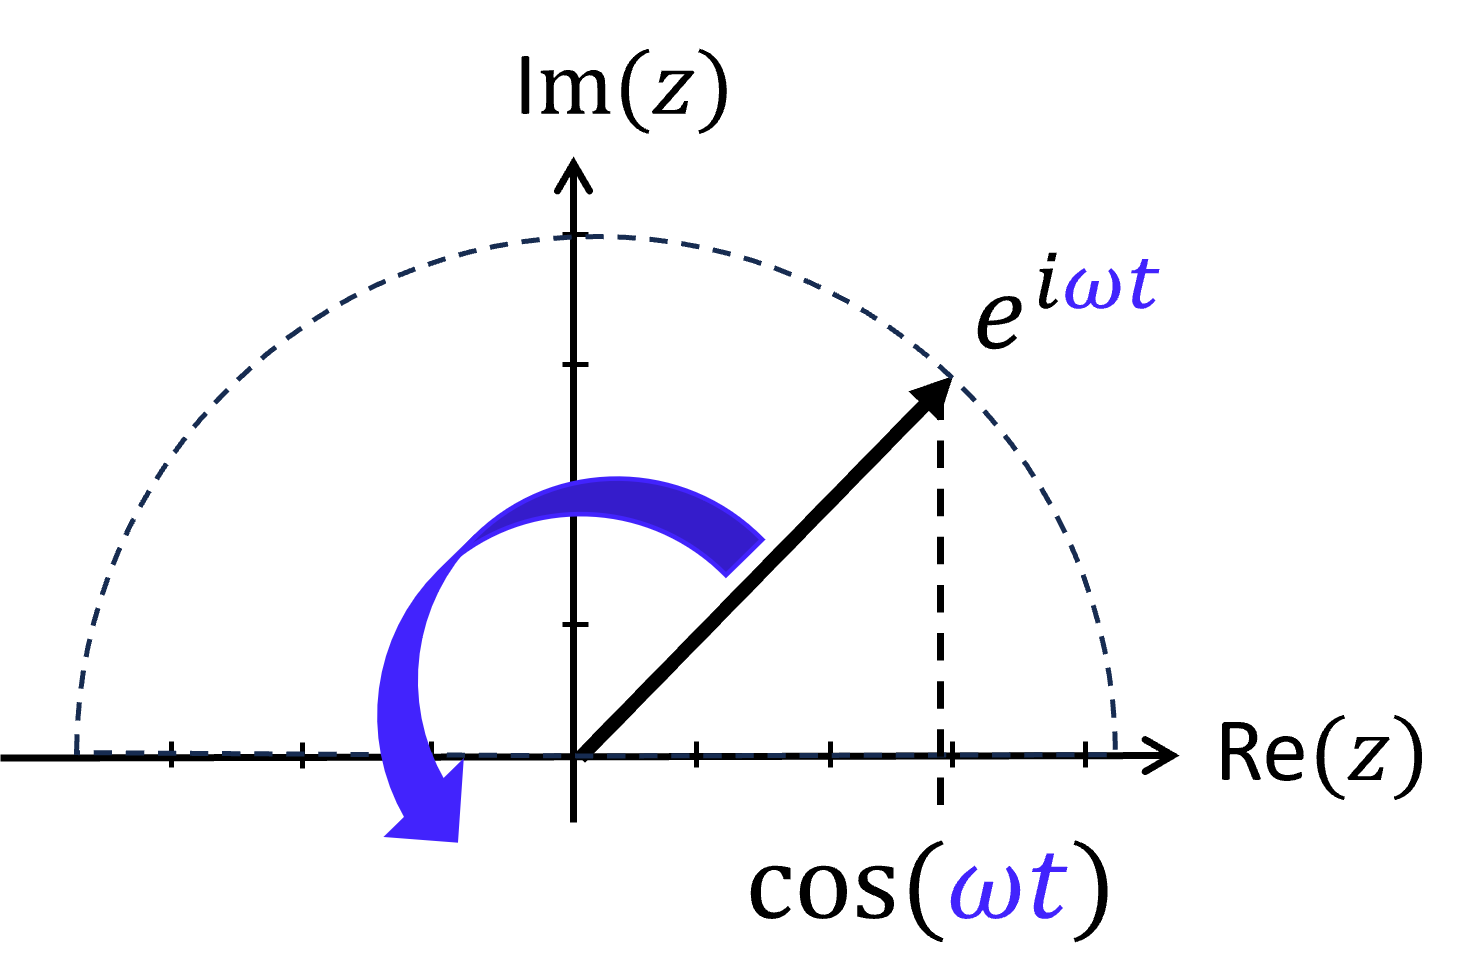
\includegraphics[width=\textwidth]{../Mathematik_1/Bilder/komplexe_zahlen_rotierender_zeiger.png}
%\end{minipage}
%\begin{minipage}{0.58\textwidth}
%
%Der komplexe Ausdruck
%\[
%e^{i\omega t}
%\]
%beschreibt einen Zeiger, der sich mit der Winkelgeschwindigkeit \(\omega\)
%auf dem Einheitskreis dreht.
%
%Sein Realteil ist
%\[
%\mathrm{Re}\left(e^{i\omega t}\right)
%=
%\cos(\omega t),
%\]
%sein Imagin�rteil
%\[
%\mathrm{Im}\left(e^{i\omega t}\right)
%=
%\sin(\omega t).
%\]
%
%Die Projektion des rotierenden Zeigers auf die reelle Achse ergibt somit eine
%Kosinusschwingung, die Projektion auf die imagin�re Achse eine
%Sinusschwingung.
%
%\end{minipage}
%
%\end{exabox}
%
%Damit erh�lt die im Kapitel �ber Funktionen untersuchte harmonische Schwingung
%eine neue geometrische Interpretation: Eine Sinus- oder Kosinusschwingung
%kann als Projektion einer gleichf�rmigen Kreisbewegung aufgefasst werden.
%
%Die komplexe Exponentialfunktion verbindet somit Rotation in der komplexen
%Ebene und harmonische Schwingung auf der reellen Achse.


%\noindent\textbf{Ausblick:}
%Die Funktionen
%\[
%t\mapsto e^{(\sigma+i\omega)t}
%\]
%verbinden exponentielles Wachstum beziehungsweise exponentielle D�mpfung mit
%einer Rotation. Dadurch k�nnen Wachstum, D�mpfung und Schwingung in einem
%einzigen mathematischen Ausdruck beschrieben werden.
%
%Diese Struktur tritt insbesondere bei der L�sung linearer
%Differentialgleichungen auf und bildet sp�ter auch eine Grundlage der
%Fourier-Analyse und der Laplace-Transformation.


\subsection{Harmonische Schwingungen und komplexe Amplituden}

Im Kapitel �ber Funktionen wurden harmonische Schwingungen in der Form
\[
s(t)
=
A\sin(\omega t+\alpha)
\]
beschrieben. Dabei bestimmt \(A\) die Amplitude, \(\omega\) die
Kreisfrequenz und \(\alpha\) die Phase.

Mithilfe der Eulerschen Formel kann dieselbe Schwingung durch eine komplexe
Exponentialfunktion dargestellt werden. Es gilt
\[
\begin{aligned}
s(t)
&=
A\sin(\omega t+\alpha)\\
&=
\mathrm{Im}
\left(
A e^{i(\omega t+\alpha)}
\right)\\
&=
\mathrm{Im}
\left(
A e^{i\alpha}e^{i\omega t}
\right).
\end{aligned}
\]

Dabei enth�lt der Faktor \(e^{i\omega t}\) die zeitabh�ngige Rotation. Die
beiden Parameter Amplitude \(A\) und Phase \(\alpha\) k�nnen dagegen in der
zeitunabh�ngigen komplexen Zahl
\[
\underline A
:=
A e^{i\alpha}
\]
zusammengefasst werden.

\begin{defbox}{Komplexe Amplitude}{ }

Die komplexe Zahl
\[
\underline A
=
A e^{i\alpha}
\]
hei�t \textbf{komplexe Amplitude} beziehungsweise \textbf{Phasor}
(\emph{phasor}).

Ihr Betrag ist die Amplitude der Schwingung,
\[
|\underline A|=A,
\]
und ihr Argument beschreibt die Phase,
\[
\arg(\underline A)=\alpha
\]
bis auf ganzzahlige Vielfache von \(2\pi\).

Die zugeh�rige Sinusschwingung kann damit in der Form
\[
s(t)
=
\mathrm{Im}
\left(
\underline A e^{i\omega t}
\right)
\]
geschrieben werden.

\end{defbox}

Diese Darstellung trennt zwei unterschiedliche Informationen voneinander:
Die gemeinsame zeitliche Rotation steckt in \(e^{i\omega t}\), w�hrend
Amplitude und Phase vollst�ndig durch die komplexe Zahl \(\underline A\)
beschrieben werden.

Gerade bei der �berlagerung mehrerer Schwingungen gleicher Frequenz f�hrt
diese Trennung zu einer erheblichen Vereinfachung.


% --------------------------------------------------------------------------
\subsubsection*{�berlagerung harmonischer Schwingungen gleicher Frequenz}

Es seien zwei harmonische Schwingungen mit derselben Kreisfrequenz
\(\omega\) gegeben. Ihre komplexen Darstellungen lauten
\[
\underline s_1(t)
=
\underline A_1e^{i\omega t}
\qquad\text{und}\qquad
\underline s_2(t)
=
\underline A_2e^{i\omega t}.
\]

Bei der Addition kann der gemeinsame zeitabh�ngige Faktor ausgeklammert
werden:
\[
\begin{aligned}
\underline s(t)
&=
\underline s_1(t)+\underline s_2(t)\\
&=
\underline A_1e^{i\omega t}
+
\underline A_2e^{i\omega t}\\
&=
(\underline A_1+\underline A_2)e^{i\omega t}.
\end{aligned}
\]

Die resultierende komplexe Amplitude ist daher einfach
\[
\underline A
=
\underline A_1+\underline A_2.
\]

\begin{theorembox}{�berlagerung gleicher Frequenz}{ }

F�r zwei komplex dargestellte harmonische Schwingungen
\[
\underline s_1(t)
=
\underline A_1e^{i\omega t},
\qquad
\underline s_2(t)
=
\underline A_2e^{i\omega t}
\]
gilt
\[
\underline s_1(t)+\underline s_2(t)
=
(\underline A_1+\underline A_2)e^{i\omega t}.
\]

Die resultierende komplexe Amplitude ist
\[
\underline A
=
\underline A_1+\underline A_2.
\]
Damit ergeben sich die Amplitude und die Phase der resultierenden Schwingung
aus
\[
A=|\underline A|
\qquad\text{und}\qquad
\alpha=\arg(\underline A).
\]

\end{theorembox}

Die �berlagerung harmonischer Schwingungen gleicher Frequenz wird damit auf
die Addition zweier komplexer Zahlen zur�ckgef�hrt. Geometrisch entspricht
dies der bereits bekannten Pfeiladdition in der Gau�schen Zahlenebene.

\begin{exabox}{Addition komplexer Amplituden}{ }

\begin{minipage}{0.4\textwidth}
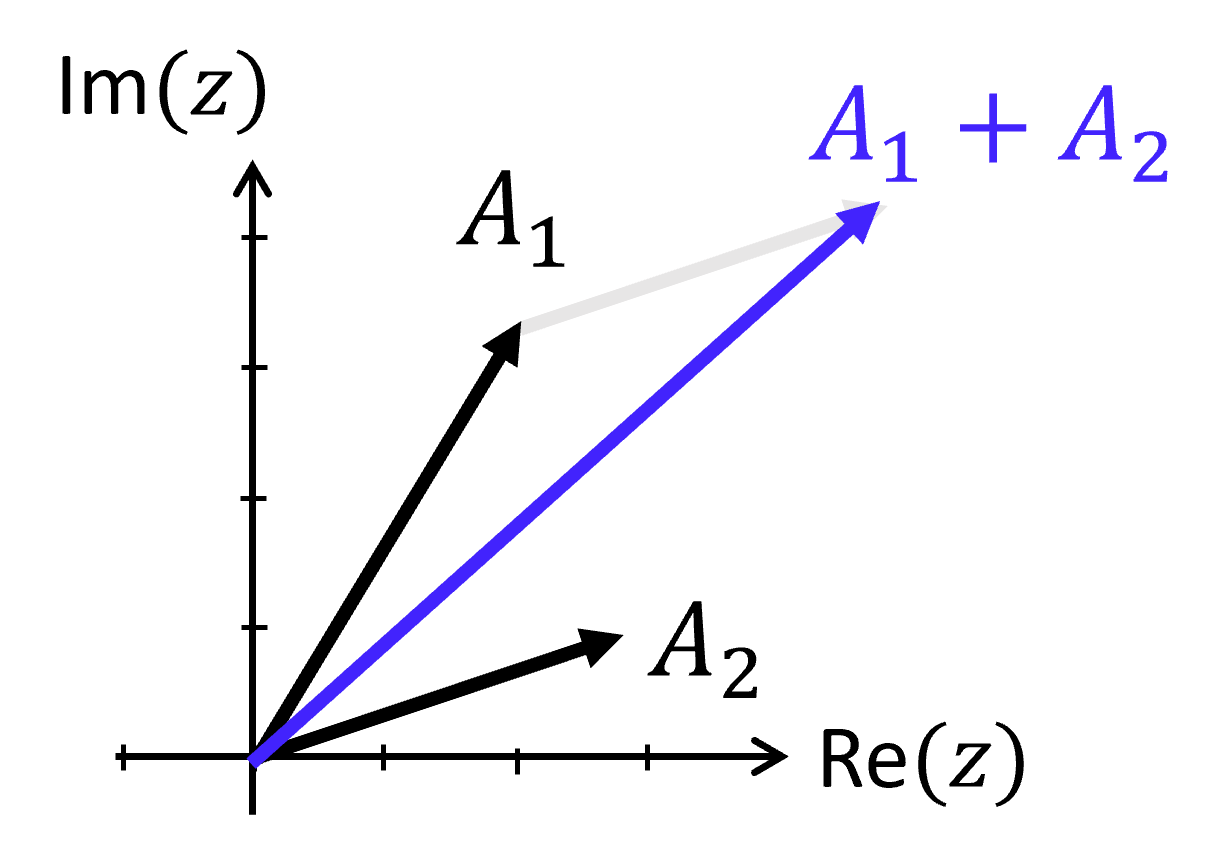
\includegraphics[width=\textwidth]{../Mathematik_1/Bilder/komplexe_zahlen_addition_komplexer_amplituden.png}
\end{minipage}
\begin{minipage}{0.58\textwidth}

Die komplexen Amplituden
\[
\underline A_1
\qquad\text{und}\qquad
\underline A_2
\]
werden als Pfeile in der komplexen Ebene dargestellt.

Ihre Summe
\[
\underline A
=
\underline A_1+\underline A_2
\]
entsteht durch Pfeiladdition.

Der Betrag des resultierenden Pfeils bestimmt die Amplitude der �berlagerten
Schwingung, sein Winkel bestimmt ihre Phase.

\end{minipage}

\end{exabox}


% --------------------------------------------------------------------------
\subsubsection*{Ein vollst�ndig gerechnetes Beispiel}

Betrachtet werden die beiden Schwingungen
\[
s_1(t)=\sin(\omega t)
\]
und
\[
s_2(t)
=
\sin\left(
\omega t+\frac{\pi}{2}
\right).
\]

F�r die erste Schwingung gilt \(A_1=1\) und \(\alpha_1=0\). Ihre komplexe
Amplitude ist daher
\[
\underline A_1
=
e^{i\cdot0}
=
1.
\]

F�r die zweite Schwingung gilt \(A_2=1\) und
\(\alpha_2=\pi/2\). Damit ergibt sich
\[
\underline A_2
=
e^{i\pi/2}
=
i.
\]

Die resultierende komplexe Amplitude lautet
\[
\underline A
=
\underline A_1+\underline A_2
=
1+i.
\]

Um daraus Amplitude und Phase der resultierenden Schwingung abzulesen, wird
\(1+i\) in Polarform dargestellt. Der Betrag ist
\[
A
=
|1+i|
=
\sqrt{1^2+1^2}
=
\sqrt2.
\]

Der Punkt \((1\,|\,1)\) liegt im ersten Quadranten und besitzt den Winkel
\[
\alpha
=
\frac{\pi}{4}.
\]
Damit gilt
\[
\underline A
=
\sqrt2\,e^{i\pi/4}.
\]

Die �berlagerung der beiden urspr�nglichen Schwingungen ergibt somit
\[
s(t)
=
\sqrt2
\sin\left(
\omega t+\frac{\pi}{4}
\right).
\]

Das Ergebnis zeigt unmittelbar den Vorteil der komplexen Darstellung. Anstatt
zwei trigonometrische Funktionen mithilfe von Additionstheoremen
zusammenzufassen, werden ihre komplexen Amplituden addiert. Betrag und Winkel
der resultierenden komplexen Zahl liefern anschlie�end Amplitude und Phase
der �berlagerten Schwingung.


% --------------------------------------------------------------------------
\subsection{Linearfaktorzerlegung �ber \(\mathbb C\)}

Die Einf�hrung der komplexen Zahlen begann mit einer algebraischen Frage:
Bestimmte Gleichungen besitzen innerhalb der reellen Zahlen keine L�sung.
Bereits eine quadratische Gleichung kann eine negative Diskriminante besitzen
und damit keine reellen Nullstellen haben.

In den komplexen Zahlen k�nnen solche Gleichungen weiter gel�st werden. So
besitzt beispielsweise
\[
z^2+6z+13=0
\]
die beiden komplexen L�sungen
\[
z_1=-3+2i
\qquad\text{und}\qquad
z_2=-3-2i.
\]

Damit l�sst sich das zugeh�rige Polynom vollst�ndig in Linearfaktoren
zerlegen:
\[
z^2+6z+13
=
(z+3-2i)(z+3+2i).
\]

Das Beispiel ist Teil eines wesentlich allgemeineren Zusammenhangs. W�hrend
ein reelles Polynom in \(\mathbb R\) nicht notwendigerweise eine Nullstelle
besitzt, ist die Situation �ber \(\mathbb C\) grundlegend anders.

\begin{theorembox}{Fundamentalsatz der Algebra}{ }

Jedes nichtkonstante Polynom mit komplexen Koeffizienten besitzt mindestens
eine komplexe Nullstelle.

Daraus folgt, dass sich jedes Polynom \(p\in\mathbb C[z]\) vom Grad
\(n\geq1\) vollst�ndig in Linearfaktoren zerlegen l�sst. Mit geeigneten
komplexen Zahlen \(z_1,\ldots,z_n\) gilt
\[
p(z)
=
a_n
(z-z_1)(z-z_2)\cdots(z-z_n).
\]

Dabei werden die Nullstellen entsprechend ihrer Vielfachheit gez�hlt. Ein
Polynom vom Grad \(n\) besitzt �ber \(\mathbb C\) somit genau \(n\)
Nullstellen, wenn Vielfachheiten ber�cksichtigt werden.

\end{theorembox}

F�r Polynome mit reellen Koeffizienten treten nichtreelle Nullstellen dabei
paarweise als komplex konjugierte Zahlen auf. Ist beispielsweise
\(a+i\,b\) mit \(b\neq0\) eine Nullstelle eines reellen Polynoms, so ist auch
\(a-i\,b\) eine Nullstelle.

Dies erkl�rt auch das vorangegangene Beispiel:
\[
-3+2i
\qquad\text{und}\qquad
-3-2i
\]
bilden ein komplex konjugiertes Paar.

Der Fundamentalsatz der Algebra schlie�t damit den Kreis zur urspr�nglichen
Motivation f�r die Einf�hrung der komplexen Zahlen. Die Erweiterung von
\(\mathbb R\) zu \(\mathbb C\) erm�glicht nicht nur die L�sung einzelner
Gleichungen wie \(z^2=-1\). Sie schafft einen Zahlenbereich, in dem jedes
nichtkonstante Polynom vollst�ndig in Linearfaktoren zerlegt werden kann.
  %  Wurzelziehene im Komplexen, Polarform, Eulersche Identit�t

\chapter{Lineare Strukturen im \(\mathbb R^n\) und \(\mathbb C^n\)}
\etocsettocstyle{\section*{Inhalt dieses Kapitels}}{}
\section*{Leitidee}

Mit dem Begriff des \textbf{Vektors} wird Geometrie algebraisch zug�nglich.
Vektoren beschreiben nicht nur Punkte oder gerichtete Gr��en im Raum. Sie
k�nnen addiert und mit Zahlen multipliziert werden und bilden dadurch eine
\textbf{lineare Struktur}.

Aus diesen beiden grundlegenden Operationen entsteht das Prinzip der
\textbf{linearen Kombination}: Vektoren k�nnen miteinander kombiniert werden,
um neue Vektoren und damit neue Richtungen oder Punkte zu erzeugen. Dadurch
lassen sich Fragen danach untersuchen, welche Vektoren aus anderen aufgebaut
werden k�nnen, welche Richtungen voneinander abh�ngig sind und welche
Vektoren gemeinsam einen Raum aufspannen. Geometrische Fragestellungen werden
auf diese Weise mit algebraischen Methoden beschreibbar.

Diese Struktur ist nicht auf den zwei- oder dreidimensionalen reellen Raum
beschr�nkt. Vektoren k�nnen aus beliebig vielen reellen oder komplexen
Komponenten bestehen und damit Elemente von
\(\mathbb R^n\) beziehungsweise \(\mathbb C^n\) sein. Der Begriff des
\textbf{Vektorraums} fasst die daf�r wesentlichen algebraischen Eigenschaften
zusammen und l�st sie von einer bestimmten Dimension oder geometrischen
Darstellung.

Mit dem \textbf{Skalarprodukt} erh�lt die lineare Struktur zus�tzlich eine
geometrische Bedeutung. Es erm�glicht, L�ngen und Winkel zu beschreiben und
f�hrt insbesondere zum Prinzip der \textbf{orthogonalen Projektion}. Ein
Vektor kann dadurch auf eine Richtung oder einen Unterraum projiziert und
dort durch einen geeigneten Vektor bestm�glich approximiert werden.

Diese Idee reicht weit �ber geometrische Vektoren hinaus. Auch andere
mathematische Objekte, insbesondere Funktionen, k�nnen Vektorr�ume bilden.
Besitzen solche R�ume zus�tzlich ein geeignetes Skalarprodukt, lassen sich
Begriffe wie Orthogonalit�t, Projektion und Approximation auf Funktionen
�bertragen. Damit entsteht eine Verbindung zwischen der linearen Algebra und
sp�teren Methoden zur Darstellung und Approximation von Funktionen.

  % Leitidee Vektoren

\bigskip
\localtableofcontents
\newpage

\setcounter{satz}{0} \setcounter{def}{0} \setcounter{exa}{0}  \section{Vektoren}\label{MA1-vektoren}

\begin{table}[H]
  \centering
  \begin{tabularx}{\textwidth}{p{0.9\textwidth} p{0.1\textwidth}}
    \toprule
	  \multicolumn{2}{c}{\textbf{�bersicht �ber Lernziele und Voraussetzungen}}\\
    \midrule
\textbf{Lernziele} &\\[.5\normalbaselineskip]
\tabitem Vektoren in \(\mathbb R^n\) und \(\mathbb C^n\) darstellen, addieren und skalieren &\\
\tabitem die Norm eines Vektors berechnen und Einheitsvektoren bestimmen &\\
\tabitem das Skalarprodukt berechnen und geometrisch interpretieren &\\
\tabitem Orthogonalit�t mithilfe des Skalarprodukts pr�fen &\\
\tabitem Vektoren orthogonal zerlegen und auf eine vorgegebene Richtung projizieren &\\
\tabitem den Winkel zwischen zwei reellen Vektoren mithilfe des Skalarprodukts bestimmen &\\
\tabitem Norm und Skalarprodukt auf Vektoren in \(\mathbb C^n\) �bertragen (+) &\\
\tabitem das Kreuzprodukt in \(\mathbb R^3\) berechnen und geometrisch interpretieren (+) &\\
    \midrule
	  \textbf{Voraussetzungen} &\\[.5\normalbaselineskip]
	  \tabitem Grundlagen & \abschnittsverweis{MA1-mengen-und-logik}-\abschnittsverweis{MA1-aequivalenzumformungen}\\
	  \tabitem Geometrie rechtwinkliges Dreieck & \abschnittsverweis{MA1-trigonometrische-funktionen}\\
	  \tabitem Komplexe Zahlen & \abschnittsverweis{MA1-komplexe-zahlen-grundlagen}\\
    \bottomrule
  \end{tabularx}
\end{table}

\ifintegriereaufgaben \noindent �bungsaufgaben zum Thema finden Sie hier: \hyperref[MA1-vektoren-aufgaben]{Aufgaben}
\vspace{0.3cm}
\hrule
\fi

\subsection{Was ist ein Vektor?} % Kapitel fr�her 

Pfeile kann man addieren und subtrahieren und man kann die L�nge von Pfeilen durch Multiplikation mit Zahlen ver�ndern:
\begin{exabox}{Pfeile}{ }
\begin{minipage}{0.5\textwidth}
	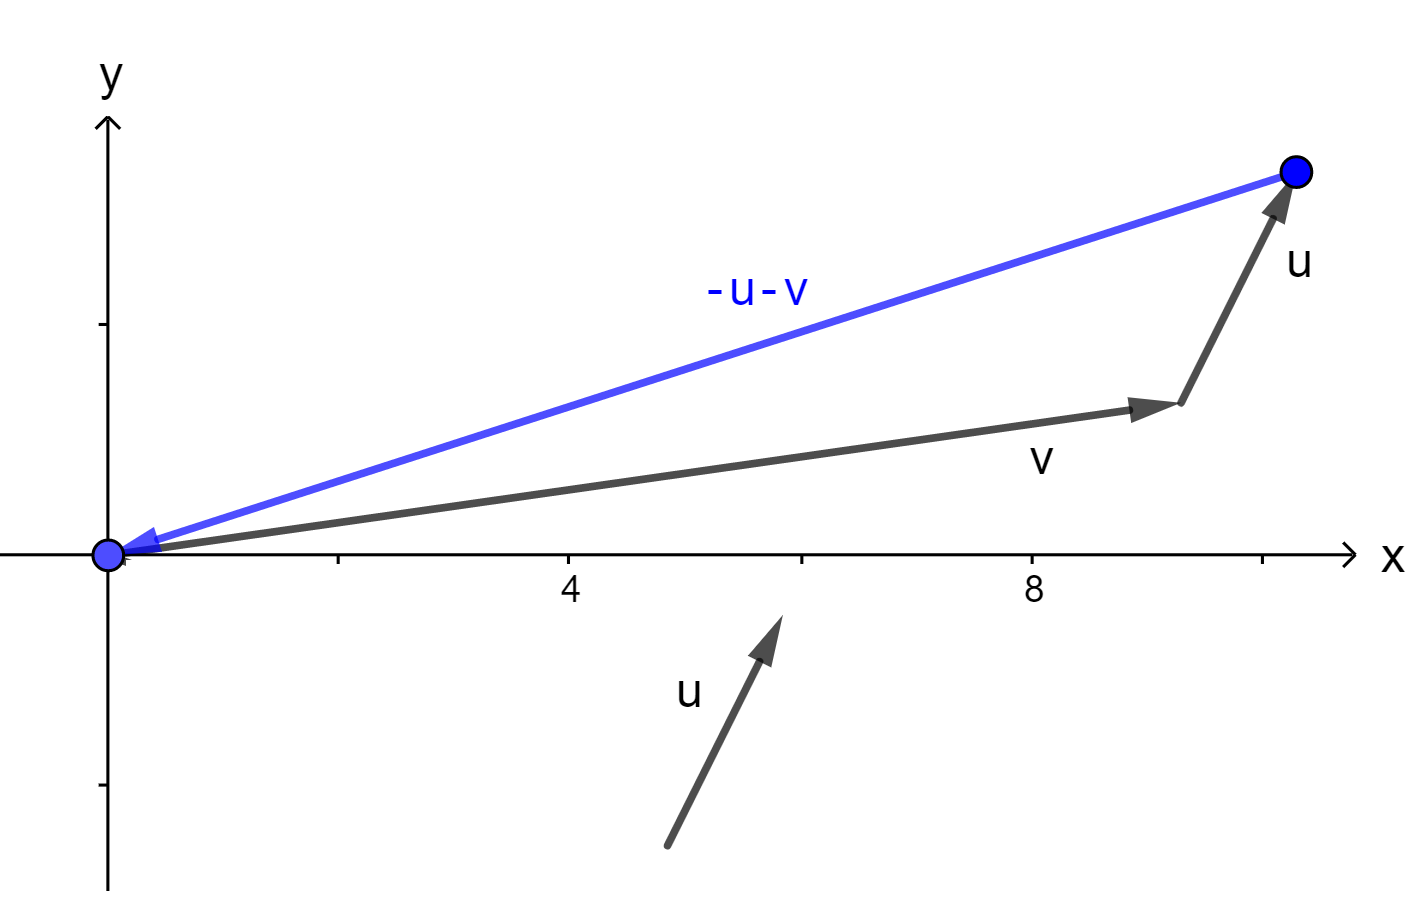
\includegraphics[width=\textwidth]{../Mathematik_1/Bilder/vektoren_pfeiladdition_gegenvektor.png}
\end{minipage}
\begin{minipage}{0.5\textwidth}
		Pfeilarithmetik kann man in \(\mathbb R^2\) gut skizzieren:
	\[ - (\vec v+\vec u) = -\vec v - \vec u  \]
\end{minipage}
\end{exabox}

Das klappt in zwei Dimensionen (Ebene) ebenso wie in drei Dimensionen (Raum). Ein Pfeil wird vollst�ndig durch seine L�nge und seine Richtung beschrieben. Um die Operation "\,Addition"\, komplett zu haben, ben�tigt man ein \underline{neutrales Element}\randverweis{MA1-zahlenmengen} der Addition. Das neutrale Element der Addition ist ein Pfeil mit L�nge Null und unbestimmter Richtung, der sogenannte Nullpfeil $\vec 0$. Es gilt: \[ \forall\, \vec a: \quad \vec a+ \vec 0= \vec a\,.\]

Zwei Pfeile werden mathematisch als gleich betrachtet, wenn sie in L�nge und Richtung �bereinstimmen: mathematisch unterscheiden sich also zwei parallel gegeneinander verschobene Pfeile nicht. Es handelt sich in der Mathematik um einen \textbf{Vektor} (\emph{vector}):
\begin{exabox}{Vektoren}{ }
\begin{minipage}{0.3\textwidth}
	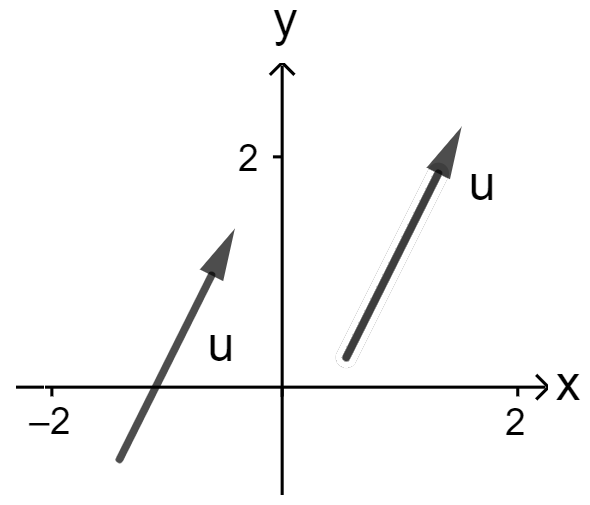
\includegraphics[width=\textwidth]{../Mathematik_1/Bilder/vektoren_gleiche_pfeile_verschoben.png}
\end{minipage}
\begin{minipage}{0.7\textwidth}
	Ein Vektor in der Mathematik ist durch die Angabe
	\begin{itemize}
		\item seiner L�nge und 
		\item seiner Richtung 
	\end{itemize}
	eindeutig bestimmt. Man darf den Vektor in der Ebene beliebig verschieben, es sind unbebundene Vektoren. 
\end{minipage}
\end{exabox}


Zwei- und dreidimensionale Vektoren werden orthographisch meist mit einem Pfeil oder unterstrichen dargestellt, also $\vec a$ oder $\underline a$, oder mit Fettbuchstab $\boldsymbol a$. Je abstrakter die Vektoren werden, um so eher benutzt man normale Buchstaben wie $a$. 

Die Vokabeln \"\,Vektor\"\, und \"\,Skalar\"\, werden nicht nur in mathematischen Zusammenh�ngen, sondern auch in der Physik st�ndig auftauchen. Es ist sinnvoll die Unterschiede zu erkl�ren:  


\vspace{0.3cm}
\noindent\textbf{Vektoren und Skalare in der Mathematik}
\begin{itemize}
	\item Vektoren in der Mathematik sind ungebundene bzw. freie Vektoren. Das Adjektiv "\,frei"\, betont, dass zwei parallele gleichlange Vektoren dieselben mathematischen Objekte sind.  
	\item Vektoren mit fixiertem Start- oder Aufh�ngepunkt \(P\) nennt man in der Mathemamtik gebundene Vektoren: 
	\item Skalare in der Mathematik sind die Zahlen, mit denen man Vektoren multiplizieren kann: also reelle oder komplexe Zahlen. Multipliziert man einen Vektor mit einer Zahl, so ver�ndert man seine L�nge, aber nicht seine Richtung - man spricht auch von Skalierung.  
\end{itemize}

\noindent\textbf{Vektoren und Skalare in der Physik}
\begin{itemize}
	\item Vektoren in der Physik sind vektorielle Gr��en wie beispielsweise der Geschwindigkeitsvektor \(\vec v\), der Impulsvektor \(\vec p\), das elektrostatische Feld \(\vec E\) oder die Newtonsche Kraft \(\vec F\)\ldots 
	\item Vektoren in der Physik, die an einem fixierten Punkt \(P\) starten, nennt man Ortsvektoren $ P + \vec v\,.$
	\item Skalare in der Physik sind ungerichtete Gr��en, beispielsweise die Masse \(m\) eines K�rpers, die Anzahl \(N\) von Teilchen, die Ladung \(q\) eines Atoms, die Energie \(E\) eines Systems oder die Raumtemperatur \(T\)\ldots 
	\item Physikalische Gr��en k�nnen nicht nur gerichtet (vektoriell) oder ungerichtet (skalar), sondern auch komplizierter sein. Zur Beschreibung der Drehung eines massebehafteten Objektes um eine bestimmte Achse braucht man den sogennanten Tr�gheitstensor \(I\). Ein Tr�gheitstensor ist kein Vektor und es ist kein Skalar, sondern eine \underline{Matrix}\randverweis{MA1-matrizen}.
	\item Jede physikalische Gr��e, ob skalar, vektoriell oder tensorwertig, besteht aus einem Zahlenwert und einer Ma�einheit. Wenn man physikalische Gesetze aufschreibt und mit physikalischen Gr��en rechnet, dann kann man immer nur Gr��en gleicher Einheit miteinander verrechnen. Deshalb ist es immer hilfreich einen Vergleich der Einheiten zu machen -  so findet man schnell heraus, ob eine Formulierung sinnvoll oder unm�glich ist:
\begin{itemize}
	\item eine Masse von $m=2.3 \, [\mathrm{ kg}]$ kann nicht mit einem Zeitintervall der L�nge $\delta t=2.3\, [\mathrm{s}]$ gleichgesetzt werden,
	\item ein Beschleunigungsvektor $\vec a = (4.2,0,0)^\intercal \, [\frac{m}{s^2}]$ kann nicht dem sklaren Druck $p=4.2\, [\mathrm{Pa}]$ entsprechen,
	\item ein Kraftvektor $\vec F \; [\mathrm{N}] = [\frac{\mathrm{kg}\cdot \mathrm{m}}{\mathrm{s}^2}]$, kann nicht gleich einem Geschwindigkeitsvektor $\vec v \; [\frac{\mathrm{m}}{\mathrm{s}}]$ sein.
\end{itemize} 
\end{itemize}

Um mit Vektoren sinnvoll rechnen zu k�nnen, dr�ckt man sie in Zahlen aus. Der Vektor, der eine Einheit nach links und drei nach oben zeigt lautet beispielsweise 
\begin{defbox}{Komponenten eines Vektors}{ }
	Ein Vektor, der eine Einheit nach links und drei nach oben zeigt lautet 
	\[ \vec a=\left( \begin{array}{c} -1 \\ 3\end{array} \right)\,. \]  
		Die Zahlen \(-1\) und \(3\) nennt man Komponenten oder Koeffizienten oder auch Eintr�ge des Vektors. 
	Entsprechend haben Vektoren im Raum drei Komponenten, beispielsweise
\[  \vec a = \left( \begin{array}{c} 2 \\ 3 \\ -4\end{array} \right)\,. \]
\end{defbox} 

Die Komponenten eines Vektors schreibt man meistens senkrecht untereinander, also als Spalte. So entsteht ein \textbf{Spaltenvektor}. Werden die Komponenten in eine Zeile geschreiben, dann spricht man von einem \textbf{Zeilenvektor}. Ein Spaltenvektore wird durch \textbf{Transposition} in einen Zeilenvektor umgewandelt. Das kleine Symbol \(^\intercal\) zeigt die Drehung an: 

\[ \left(  -1, 3\right)^\intercal = \left( \begin{array}{c} -1 \\3\end{array}\right) \quad \textnormal{bzw.} \quad \left(  2, 3, -4\right)^\intercal = \left( \begin{array}{c} 2 \\ 3 \\ -4\end{array}\right)\,. \]  

\begin{exabox}{Rechnen mit Vektoren in der Ebene}{ }
	\begin{itemize}
		\item Man skaliert einen Vektor, indem man jede Komponente des Vektors mit dem Skalar multipliziert:  
\[ 
	2 \cdot \vec a= 2\cdot \left( \begin{array}{c} -1 \\ 3\end{array} \right) = \left( \begin{array}{c} 2\cdot (-1) \\ 2\cdot 3\end{array} \right) = \left( \begin{array}{c} -2 \\ 6\end{array} \right)\,.
\]
\item Man addiert zwei Vektoren, indem man die Komponenten der Vektoren zeilenweise addiert: 
  \[  
  \vec a + \vec b = \left( \begin{array}{c} -1 \\ 3\end{array} \right)  + \left( \begin{array}{c} 4 \\ 2\end{array} \right) =  \left( \begin{array}{c} 3 \\ 5\end{array} \right) \,.
  \]
	\end{itemize}
\end{exabox} 

\noindent\textbf{Bemerkungen:}
\begin{itemize}
	\item Die Bedeutung der Komponenten h�ngt von der Wahl des Ursprungs und der Achsen ab! 
	\item Der Nullvektor $\vec 0$ ist der Vektor, bei dem alle Komponenten gleich null sind.
\end{itemize}

Die Menge aller Vektoren mit zwei reellen Komponenten wird mit $\mathbb R^2$ bezeichnet und die Menge aller Vektoren mit drei reellen Komponenten ist entsprechend $\mathbb R^3$.
Allgemein schreibt man
\[
\mathbb R^n = \mathbb R \times \mathbb R \times \dots \times \mathbb R ,
\]
das sogenannte $n$-fache kartesische Produkt der reellen Zahlen.

Das Wort "\,identifizieren"\, resultiert aus der Tatsache, dass die Mengen $\mathbb R^n, \; n \in \mathbb N^+$, ein Doppelleben f�hren: man kann jedes Element des $\mathbb R^2$ entweder als Punkt $(x\,|\,y)$ in der Ebene oder als Vektor $(x,y)^\intercal$ auffassen. 
\begin{defbox}{$\mathbb R^2$ als Menge von Vektoren}{ }
	\[ \mathbb R^2 = \left\{ \left( \begin{array}{c}  x \\ y \end{array}\right)\, \textnormal{mit}\; x,y\in \mathbb R\right\} \]
\end{defbox}
Aus dem Zusammenhang wird klar, welchen Standpunkt man einnimmt. %Im Englisch sprachigen Raum schreibt man Punkte in der Form $(2,3)$, was im Deutschen zu Verwechselungen mit dem Dezimalkomma f�hren kann.
Die einfachste �bersetzung zwischen Punkten und Vektoren ergibt sich wie folgt
\begin{exabox}{Vektor vs. Punkt}{ }
	$ \left( \begin{array}{c}  2 \\ 3 \end{array}\right) = (2\, | \,3) - (0\,|\,0)\,, $
\end{exabox}
wobei nun links explizit ein gebundener Vektor mit Aufh�ngepunkt im Ursprung steht.

Kommen wir nochmal zur�ck auf die Definition eines Vektors: ein freier Vektor ist durch seine L�nge und seine Richtung eindeutig bestimmt. Das bedeutet, dass die Angabe dieser Informationen gen�gt, um den Vektor zu kennen! 
\[ \textnormal{Vektor}\quad   \Leftrightarrow \quad  \left( \,\textnormal{L"ange, Richtung} \,\right) \]
F�r die L�nge $\| \vec a\| $ oder $|\vec a|$ eines  Vektors $\vec a\in\mathbb R^2$ gilt\marginpar{\small Warum?}:
  \[
  \begin{array}{rcl}
	  \vec a = \left( \begin{array}{c} 2 \\ -4\end{array} \right) \quad \Rightarrow \|\vec a\| := \sqrt{ 2^2+(-4)^2} = \sqrt{20} \,.
\end{array}
\]
Zur Angabe der Richtungsinformation von \(\vec a\) bietet sich ein Vektor an, der in Richtung von \(\vec a\) zeigt und dessen L�nge zu eins normiert ist, der also keine spezifische L�ngeninformation �ber \(\vec a\) besitzt! 

\begin{defbox}{Einheitsvektor}{ }
	Zu einem gegebenen Vektor \(\vec a \not = \vec 0\) ist \(\hat a\) der zugeh�rigen \textbf{Einheitsvektor}, wobei
$$
\hat a:= \dfrac{\vec a}{\|\vec a\|}\,.
$$
\end{defbox}

Das Konzept der Vektoren in der Ebene ist sehr zug�nglich, weil wir uns die Vektoren vorstellen k�nnen. Allerdings hindert uns nichts daran das Konzept zu erweitern, beispielsweise auf \(\mathbb R^n\).  

\begin{defbox}{Vektoren in \(\mathbb R^n\) }{ }
	Ein \(n\)-Tupel reeller Zahlen \(a_k, \, k=1,\dots,n\) definiert einen Vektor in \(\mathbb R^n\) mit \(n\) Komponenten: 
\[  \vec a = \left( a_1, a_2, \cdots, a_n\right)^\intercal\,. \]
Ein nicht-trivialer Vektor, \(\vec a \not = \vec 0\), ist durch seine L�nge und seine Richtung eindeutig festgelegt:
\[ \vec a\quad   \Leftrightarrow \quad  \left( \|\vec a\| ,  \hat a\right)\,, \quad \textnormal{mit}\quad \begin{cases}\left\| \vec a \right\| &= \displaystyle{\sqrt{ \sum\limits_{k=1}^n a_k^2}} \geq 0\in \mathbb R\,, \\ \hat a &= \dfrac{\vec a}{\|\vec a\|}\,,\end{cases}\]
und es gilt 
\[ \vec a = \|\vec a\| \cdot\hat a\,.\]
\end{defbox}

\subsection{Skalarprodukt}

Vektoren k�nnen addiert und mit Skalaren multipliziert werden. Damit lassen
sich bereits viele geometrische Operationen algebraisch beschreiben. Eine
wesentliche geometrische Information ist damit jedoch noch nicht unmittelbar
zug�nglich: die Lage zweier Vektoren relativ zueinander.

Insbesondere stellt sich die Frage, wie algebraisch erkannt werden kann, ob
zwei Vektoren in dieselbe Richtung zeigen, senkrecht aufeinander stehen oder
einen bestimmten Winkel miteinander einschlie�en.

Eine solche Information kann nicht durch Addition oder skalare
Multiplikation allein gewonnen werden. Daf�r wird eine weitere Verkn�pfung
ben�tigt, die zwei Vektoren eine Zahl zuordnet. Diese Verkn�pfung ist das
\textbf{Skalarprodukt} (\emph{inner product}).

Auch in der Physik tritt genau eine solche Verkn�pfung auf. Bei der
mechanischen Arbeit ist nicht nur die Gr��e einer Kraft und eines Weges
entscheidend, sondern auch deren relative Richtung. Eine Kraft, die senkrecht
zur Bewegungsrichtung wirkt, verrichtet entlang dieses Weges keine Arbeit.
Das Skalarprodukt erfasst genau diese Richtungsinformation.

\begin{defbox}{Skalarprodukt in \(\mathbb R^n\)}{ }

F�r zwei Vektoren
\[
\vec a
=
(a_1,\ldots,a_n)^\intercal,
\qquad
\vec b
=
(b_1,\ldots,b_n)^\intercal
\]
in \(\mathbb R^n\) ist das Skalarprodukt definiert durch
\[
\langle\vec a,\vec b\rangle
=
\sum_{k=1}^{n}a_kb_k.
\]

Das Ergebnis des Skalarprodukts ist \emph{kein} Vektor, sondern eine reelle
Zahl:
\[
\langle\vec a,\vec b\rangle\in\mathbb R.
\]

\noindent\textbf{Bemerkung zur Schreibweise:}
F�r das Skalarprodukt sind verschiedene Schreibweisen gebr�uchlich. Neben
\(\langle\vec a,\vec b\rangle\) wird insbesondere auch ein ausgef�llter
Punkt verwendet oder ein kleines Malzeichen,
\[
	\vec a\bullet\vec b, \quad  \vec a \cdot \vec b\,.
\]
\end{defbox}

Die Berechnung erfolgt komponentenweise. Entsprechende Komponenten werden
multipliziert und die entstehenden Produkte anschlie�end addiert. F�r
\[
\vec a
=
\begin{pmatrix}
3\\4\\5
\end{pmatrix},
\qquad
\vec b
=
\begin{pmatrix}
2\\-3\\1
\end{pmatrix}
\]
ergibt sich beispielsweise
\[
\langle\vec a,\vec b\rangle
=
3\cdot2+4\cdot(-3)+5\cdot1
=
-1.
\]

Neben der Schreibweise
\(\langle\vec a,\vec b\rangle\) ist insbesondere in
\(\mathbb R^n\) auch die Schreibweise
\(\vec a\cdot\vec b\) gebr�uchlich.


\begin{theorembox}{Eigenschaften des Skalarprodukts}{ }

F�r \(\vec a,\vec b,\vec c\in\mathbb R^n\) und
\(\lambda\in\mathbb R\) gilt
\[
\langle\vec a,\vec b\rangle
=
\langle\vec b,\vec a\rangle,
\]
\[
\langle\vec a,\vec b+\vec c\rangle
=
\langle\vec a,\vec b\rangle
+
\langle\vec a,\vec c\rangle
\]
sowie
\[
\langle\lambda\cdot \vec a,\vec b\rangle
=
\langle\vec a,\lambda\cdot \vec b\rangle
=
\lambda\cdot \langle\vec a,\vec b\rangle.
\]

Das reelle Skalarprodukt ist damit symmetrisch und linear in beiden
Argumenten.

\end{theorembox}


\subsubsection*{Skalarprodukt und L�nge}

Eine erste Verbindung zwischen dem Skalarprodukt und der Geometrie entsteht,
wenn ein Vektor mit sich selbst multipliziert wird. F�r
\(\vec a\in\mathbb R^n\) gilt
\[
\langle\vec a,\vec a\rangle
=
a_1^2+\cdots+a_n^2.
\]
Der Ausdruck auf der rechten Seite ist gerade das Quadrat der euklidischen
L�nge von \(\vec a\).

\begin{theorembox}{Relation zwischen Norm und Skalarprodukt}{ }

F�r jeden Vektor \(\vec a\in\mathbb R^n\) gilt
\[
\|\vec a\|^2
=
\langle\vec a,\vec a\rangle
\]
und damit
\[
\|\vec a\|
=
\sqrt{\langle\vec a,\vec a\rangle}.
\]

\end{theorembox}

Das Skalarprodukt enth�lt damit bereits die Information �ber die L�nge eines
Vektors. Entscheidend ist jedoch, dass es dar�ber hinaus auch die relative
Richtung zweier verschiedener Vektoren erfasst.

\subsubsection*{Projektion und Winkel zwischen Vektoren}

Orthogonalit�t beschreibt zun�chst nur den besonderen Fall eines Winkels von
\(90^\circ\). In der Ebene und im dreidimensionalen Raum l�sst sich jedoch
auch der Winkel zwischen zwei beliebigen Vektoren geometrisch betrachten.

Ausgangspunkt ist zun�chst die anschauliche Situation in der Ebene. Gesucht
ist der Anteil eines Vektors \(\vec b\), der in Richtung eines zweiten
Vektors \(\vec a\) zeigt. Dazu wird \(\vec b\) in zwei zueinander
orthogonale Anteile zerlegt: einen Anteil \(\vec b_{\parallel}\), der
parallel zu \(\vec a\) verl�uft, und einen Anteil \(\vec b_{\perp}\), der
senkrecht auf \(\vec a\) steht.

\vspace{0.5cm}
\begin{center}
\begin{minipage}{0.3\textwidth}
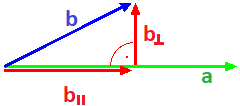
\includegraphics[width=\textwidth]{../Mathematik_1/Bilder/vektoren_orthogonale_zerlegung.png}
\end{minipage}
\begin{minipage}{0.6\textwidth}
\[
\textcolor{blue}{\vec b}
=
\textcolor{red}{\vec b_{\parallel}}
+
\textcolor{red}{\vec b_{\perp}},
\qquad
\left\langle
\textcolor{red}{\vec b_{\perp}},
\textcolor{darkgreen}{\vec a}
\right\rangle
=
0.
\]
\end{minipage}
\end{center}
\vspace{0.5cm}

Der parallele Anteil enth�lt genau die Information dar�ber, wie stark
\(\vec b\) in Richtung von \(\vec a\) zeigt.

Zun�chst seien \(\vec a,\vec b\in\mathbb R^2\) zwei von Null verschiedene
Vektoren und \(\alpha\in[0,\pi]\) ihr geometrisch eingeschlossener Winkel.
Ist \(\alpha\) spitz, so zeigt der parallele Anteil in Richtung von
\(\vec a\). Seine L�nge betr�gt nach der bekannten Geometrie des
rechtwinkligen Dreiecks \(\|\vec b\|\cos(\alpha)\). Mit dem Einheitsvektor
\(\hat a=\vec a/\|\vec a\|\) folgt daher
\[
\vec b_{\parallel}
=
\|\vec b\|\cos(\alpha)\,\hat a
=
\frac{\|\vec b\|}{\|\vec a\|}
\cos(\alpha)\,\vec a.
\]

Bei einem stumpfen Winkel ist \(\cos(\alpha)<0\). Der parallele Anteil zeigt
dann entgegen der Richtung von \(\vec a\). Dieselbe Formel beschreibt somit
beide F�lle.

Diese geometrische Zerlegung erm�glicht nun, das Skalarprodukt zu
interpretieren. Da
\(\vec b=\vec b_{\parallel}+\vec b_{\perp}\) und
\(\vec b_{\perp}\perp\vec a\), gilt
\[
\begin{array}{rcl l}
\big\langle\vec a,\vec b\big\rangle
&=&
\big\langle\vec a,\vec b_{\parallel}+\vec b_{\perp}\big\rangle & \quad \text{Orthogonale Zerlegung f�r } \vec b \text{ einsetzen} \\[0.5ex]
&=& \big\langle\vec a,\vec b_{\parallel}\big\rangle + \underbrace{\big\langle\vec a,\vec b_{\perp}\big\rangle}_{\displaystyle{=0} } & \quad \text{Eigenschaften des Skalarprodukts ausnutzen}\\[0.5ex]
&=& \big\langle \vec a, \frac{\|\vec b\|}{\|\vec a\|} \cdot \cos(\alpha)\cdot \vec a \big\rangle &\quad \text{Darstellung f�r } \vec b_\parallel \text{ einsetzen}\\[0.5ex] 
&=& \frac{\|\vec b\|}{\|\vec a\|}\cdot \cos(\alpha)\cdot \underbrace{\langle\vec a,\vec a\rangle}_{=\|\vec a\|^2} &\quad \text{Eigenschaften des Skalarprodukts ausnutzen} \\[0.5ex]
&=& \|\vec a\|\cdot\|\vec b\|\cdot \cos(\alpha). & \end{array}
\]

Damit ist f�r Vektoren in der Ebene eine Verbindung zwischen dem geometrisch bekannten Winkel und dem algebraisch berechenbaren Skalarprodukt gefunden:
\[
\cos(\alpha) = \frac{\langle\vec a,\vec b\rangle}{\|\vec a\|\cdot \|\vec b\|}.
\]

Diese Formel besitzt eine weitergehende Bedeutung. Ihre rechte Seite enth�lt nur das Skalarprodukt und die Norm der beiden Vektoren. Beide Begriffe sind bereits f�r Vektoren in \(\mathbb R^n\) definiert und ben�tigen keine zweidimensionale geometrische Darstellung.

Damit kann der aus der Ebene bekannte Winkelbegriff auf beliebige reelle Vektorr�ume \(\mathbb R^n\) �bertragen werden.

\begin{defbox}{Winkel zwischen Vektoren in \(\mathbb R^n\)}{ }

F�r zwei von Null verschiedene Vektoren
\(\vec a,\vec b\in\mathbb R^n\) wird der \textbf{Winkel}
\(\alpha\in[0,\pi]\) zwischen den beiden Vektoren durch
\[
\cos(\alpha)
:=
\frac{\langle\vec a,\vec b\rangle}
{\|\vec a\|\,\|\vec b\|}
\]
definiert.

�quivalent dazu gilt
\[
\alpha
=
\arccos\left(
\frac{\langle\vec a,\vec b\rangle}
{\|\vec a\|\,\|\vec b\|}
\right).
\]

F�r \(n=2\) und \(n=3\) stimmt diese Definition mit dem geometrisch
anschaulichen Winkel zwischen zwei Vektoren �berein.

\end{defbox}

Die Definition erweitert damit einen aus der ebenen und r�umlichen Geometrie
bekannten Begriff auf Dimensionen, in denen eine unmittelbare geometrische
Vorstellung nicht mehr zur Verf�gung steht. Ein Winkel zwischen zwei
Vektoren in \(\mathbb R^{10}\) oder \(\mathbb R^{100}\) l�sst sich nicht mehr
als Winkel zweier gezeichneter Pfeile veranschaulichen; �ber das
Skalarprodukt ist er dennoch eindeutig definiert.

%Die Winkelformel ist damit in der Ebene eine Konsequenz der geometrischen Interpretation des Skalarprodukts und wird anschlie�end zur Definition des Winkelbegriffs in \(\mathbb R^n\).

Gleichzeitig liefert dieselbe Beziehung die \textbf{vorzeichenbehaftete
Projektionsl�nge} von \(\vec b\) in Richtung von \(\vec a\). F�r den
Einheitsvektor \(\hat a\) gilt
\[
\langle\vec b,\hat a\rangle
=
\|\vec b\|\cos(\alpha).
\]
Dieser Wert beschreibt, wie stark \(\vec b\) in Richtung von
\(\vec a\) beziehungsweise bei negativem Vorzeichen in die
entgegengesetzte Richtung zeigt.

\begin{theorembox}{Orthogonale Projektion auf eine Richtung}{ }

F�r \(\vec a\neq\vec 0\) l�sst sich \(\vec b\) orthogonal zerlegen als
\[
\vec b
=
\vec b_{\parallel}
+
\vec b_{\perp} \quad \text{ mit } \vec b_{\perp}\perp\vec a.
\]
Der zu \(\vec a\) parallele Vektor ist
\[
\vec b_{\parallel}
=
\langle\vec b,\hat a\rangle\cdot \hat a
=
\frac{\langle\vec b,\vec a\rangle}
{\|\vec a\|^2} \cdot \vec a
\]
und der zu \(\vec a\) orthogonale Vektor ist
\[
\vec b_{\perp}
=
\vec b-\vec b_{\parallel}.
\]

\end{theorembox}

Das Skalarprodukt beantwortet damit mehrere zun�chst unterschiedliche
geometrische Fragen mit derselben algebraischen Operation: Es beschreibt
Orthogonalit�t, erm�glicht die orthogonale Projektion und erweitert den
geometrischen Winkelbegriff auf Vektoren in beliebigen Dimensionen.

Die Projektion wird sp�ter noch eine weitergehende Bedeutung erhalten. Wird
nicht nur auf eine einzelne Richtung, sondern auf einen ganzen Unterraum
projiziert, entsteht dort die bestm�gliche orthogonale Approximation eines
Vektors.

\subsubsection*{Vektoren in \(\mathbb C^n\)}

Die bisherigen �berlegungen bezogen sich auf Vektoren mit reellen
Komponenten. Nach der Einf�hrung der komplexen Zahlen liegt es nahe, auch
Vektoren
\[
\vec u
=
(u_1,\ldots,u_n)^\intercal
\in\mathbb C^n
\]
zu betrachten.

Addition und skalare Multiplikation werden wie in \(\mathbb R^n\)
komponentenweise durchgef�hrt. Bei der �bertragung des Skalarprodukts ist
jedoch eine Anpassung notwendig. W�rden komplexe Komponenten einfach
miteinander multipliziert, w�re insbesondere
\(\langle\vec u,\vec u\rangle\) im Allgemeinen keine
nichtnegative reelle Zahl und k�nnte daher nicht als Quadrat einer L�nge
interpretiert werden.

Deshalb wird eine der beiden Komponenten im Skalarprodukt komplex konjugiert.

\begin{defbox}{Skalarprodukt und Norm in \(\mathbb C^n\)}{ }

F�r
\[
\vec u
=
(u_1,\ldots,u_n)^\intercal,
\qquad
\vec v
=
(v_1,\ldots,v_n)^\intercal
\]
in \(\mathbb C^n\) wird das Skalarprodukt hier durch
\[
\langle\vec u,\vec v\rangle
=
\sum_{k=1}^{n}\overline{u_k}\,v_k
\]
definiert.

F�r die Norm folgt
\[
\|\vec u\|
=
\sqrt{\langle\vec u,\vec u\rangle}
=
\sqrt{
\sum_{k=1}^{n}|u_k|^2
}.
\]

\end{defbox}

Im Unterschied zum reellen Skalarprodukt ist das komplexe Skalarprodukt im
Allgemeinen nicht symmetrisch, sondern \textbf{konjugiert symmetrisch}:
\[
\langle\vec u,\vec v\rangle
=
\overline{
\langle\vec v,\vec u\rangle
}.
\]

Mit der hier verwendeten Konvention ist es im ersten Argument
konjugiert-linear und im zweiten Argument linear.

Orthogonalit�t l�sst sich dagegen unmittelbar �bertragen:
\[
\vec u\perp\vec v
\quad\Longleftrightarrow\quad
\langle\vec u,\vec v\rangle=0.
\]

Eine �bertragung der reellen Winkelformel
% \[
% \cos(\alpha)
% =
% \frac{\langle\vec u,\vec v\rangle}
% {\|\vec u\|\,\|\vec v\|}
% \]
ist dagegen nicht m�glich, da das komplexe Skalarprodukt im Allgemeinen
selbst komplexwertig ist.

\noindent\textbf{Bemerkung:}
In der Literatur werden zwei Konventionen f�r komplexe Skalarprodukte
verwendet. Bei der hier verwendeten Konvention wird das erste Argument
konjugiert; andere Darstellungen konjugieren das zweite Argument. Beide
Konventionen f�hren zur gleichen Norm und beschreiben dieselbe
Orthogonalit�tsstruktur, m�ssen innerhalb einer Rechnung jedoch konsequent
verwendet werden.

\subsection{Kreuzprodukt (+)}

Das Skalarprodukt ordnet zwei Vektoren eine Zahl zu und erm�glicht dadurch Aussagen �ber L�nge, Orthogonalit�t, Projektion und Winkel. Im dreidimensionalen Raum (und nur da!) tritt daneben eine zweite wichtige Verkn�pfung von Vektoren auf, deren Ergebnis wiederum ein Vektor ist.

Ausgangspunkt ist die folgende geometrische Frage: Zu zwei Vektoren
\(\vec a,\vec b\in\mathbb R^3\) wird ein Vektor gesucht, der
senkrecht auf beiden Vektoren steht. Eine solche Richtung ist beispielsweise
f�r die Beschreibung einer Ebene im Raum oder einer Drehachse von Bedeutung.

Das \textbf{Kreuzprodukt} (\emph{cross product}) liefert genau einen solchen
Vektor und enth�lt dar�ber hinaus Information �ber die von
\(\vec a\) und \(\vec b\) aufgespannte Fl�che.

\begin{theorembox}{Geometrische Eigenschaften des Kreuzprodukts}{ }

F�r zwei Vektoren
\(\vec a,\vec b\in\mathbb R^3\) besitzt das Kreuzprodukt
\[
\vec a\times\vec b
\]
die folgenden geometrischen Eigenschaften.

\begin{minipage}{0.4\textwidth}
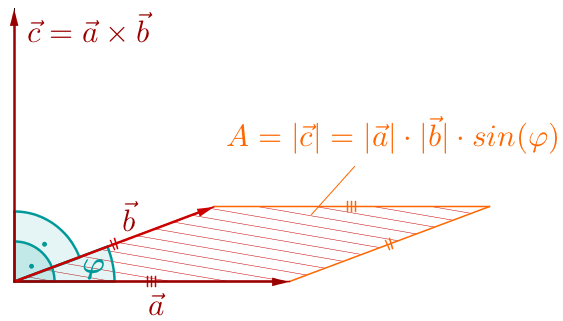
\includegraphics[width=\textwidth]{../Mathematik_1/Bilder/vektoren_kreuzprodukt_parallelogrammflaeche.png}
\end{minipage}
\begin{minipage}{0.56\textwidth}

Der Vektor \(\vec a\times\vec b\) steht senkrecht auf beiden
Ausgangsvektoren:
\[
\langle
\vec a\times\vec b,
\vec a
\rangle
=
0
\]
und
\[
\langle
\vec a\times\vec b,
\vec b
\rangle
=
0.
\]

Seine Richtung wird durch die Orientierung von
\(\vec a\) und \(\vec b\) festgelegt. Die Vektoren
\[
\vec a,\quad
\vec b,\quad
\vec a\times\vec b
\]
bilden in dieser Reihenfolge ein Rechtssystem. Die Richtung kann mit der
Rechte-Hand-Regel bestimmt werden.

\end{minipage}

Seine L�nge betr�gt
\[
\|\vec a\times\vec b\|
=
\|\vec a\|\,\|\vec b\|\sin(\varphi),
\]
wobei \(\varphi\in[0,\pi]\) der Winkel zwischen
\(\vec a\) und \(\vec b\) ist.

\end{theorembox}

Die Formel f�r die L�nge besitzt eine unmittelbare geometrische Bedeutung.
Die Vektoren \(\vec a\) und \(\vec b\) spannen ein
Parallelogramm auf. Wird \(\vec a\) als Grundseite gew�hlt, so besitzt
dieses Parallelogramm die H�he
\(\|\vec b\|\sin(\varphi)\). Sein Fl�cheninhalt ist daher
\[
A
=
\|\vec a\|\,
\|\vec b\|\sin(\varphi)
=
\|\vec a\times\vec b\|.
\]

Der Betrag des Kreuzprodukts entspricht somit dem Fl�cheninhalt des von den
beiden Vektoren aufgespannten Parallelogramms. F�r den Fl�cheninhalt des
zugeh�rigen Dreiecks gilt entsprechend
\[
A_\triangle
=
\frac12\|\vec a\times\vec b\|.
\]

\begin{defbox}{Berechnung des Kreuzprodukts}{ }

F�r
\[
\vec a
=
\begin{pmatrix}
a_1\\a_2\\a_3
\end{pmatrix},
\qquad
\vec b
=
\begin{pmatrix}
b_1\\b_2\\b_3
\end{pmatrix}
\]
ist das Kreuzprodukt definiert durch
\[
\vec a\times\vec b
=
\begin{pmatrix}
a_2\cdot b_3-a_3\cdot b_2\\
a_3\cdot b_1-a_1\cdot b_3\\
a_1\cdot b_2-a_2\cdot b_1
\end{pmatrix}.
\]

\end{defbox}

Die Reihenfolge der beiden Vektoren ist wesentlich. Beim Vertauschen der
Faktoren �ndert sich die Orientierung und damit das Vorzeichen:
\[
\vec b\times\vec a
=
-\vec a\times\vec b.
\]
Das Kreuzprodukt ist also nicht kommutativ.

\begin{exabox}{Kreuzprodukt zweier Vektoren}{ }

Gegeben seien
\[
\vec a
=
\begin{pmatrix}
3\\4\\5
\end{pmatrix},
\qquad
\vec b
=
\begin{pmatrix}
2\\-3\\1
\end{pmatrix}.
\]

Das Kreuzprodukt ergibt sich zu
\[
\begin{aligned}
\vec a\times\vec b
&=
\begin{pmatrix}
4\cdot1-5\cdot(-3)\\
5\cdot2-3\cdot1\\
3\cdot(-3)-4\cdot2
\end{pmatrix}\\[1ex]
&=
\begin{pmatrix}
19\\7\\-17
\end{pmatrix}.
\end{aligned}
\]

Die geometrische Bedeutung kann unmittelbar mithilfe des Skalarprodukts
�berpr�ft werden. F�r den ersten Ausgangsvektor gilt
\[
\begin{aligned}
\left\langle
\begin{pmatrix}3\\4\\5\end{pmatrix},
\begin{pmatrix}19\\7\\-17\end{pmatrix}
\right\rangle
&=
3\cdot19+4\cdot7+5\cdot(-17)\\
&=
57+28-85\\
&=
0.
\end{aligned}
\]

F�r den zweiten Ausgangsvektor ergibt sich entsprechend
\[
\begin{aligned}
\left\langle
\begin{pmatrix}2\\-3\\1\end{pmatrix},
\begin{pmatrix}19\\7\\-17\end{pmatrix}
\right\rangle
&=
2\cdot19-3\cdot7-17\\
&=
38-21-17\\
&=
0.
\end{aligned}
\]

Der berechnete Vektor steht somit tats�chlich senkrecht auf
\(\vec a\) und auf \(\vec b\).

Seine L�nge ist
\[
\|\vec a\times\vec b\|
=
\sqrt{19^2+7^2+(-17)^2}
=
\sqrt{699}.
\]
Damit betr�gt auch der Fl�cheninhalt des von
\(\vec a\) und \(\vec b\) aufgespannten Parallelogramms
\(\sqrt{699}\).

\end{exabox}


\subsubsection*{Typische Anwendungen des Kreuzprodukts}

Die geometrischen Eigenschaften des Kreuzprodukts f�hren unmittelbar zu
mehreren wichtigen Anwendungen.

Soll zu zwei nicht parallelen Vektoren
\(\vec a,\vec b\in\mathbb R^3\) eine Richtung bestimmt werden,
die auf beiden senkrecht steht, liefert
\[
\vec c
=
\vec a\times\vec b
\]
eine solche Richtung.

Auch Parallelit�t kann mithilfe des Kreuzprodukts gepr�ft werden. F�r zwei
Vektoren gilt
\[
\vec a\parallel\vec b
\quad\Longleftrightarrow\quad
\vec a\times\vec b=\vec 0.
\]
Denn bei parallelen oder antiparallelen Vektoren ist der eingeschlossene
Winkel \(0\) beziehungsweise \(\pi\), sodass
\(\sin(\varphi)=0\) und damit
\(\|\vec a\times\vec b\|=0\).

Schlie�lich liefert die L�nge des Kreuzprodukts den Fl�cheninhalt des aufgespannten Parallelogramms. 
  % Vektoren
\newpage
\setcounter{satz}{0} \setcounter{def}{0} \setcounter{exa}{0}  \section{Vektorraum}\label{MA1-vektorraum}

\begin{table}[H]
  \centering
  \begin{tabularx}{\textwidth}{p{0.9\textwidth} p{0.1\textwidth}}
    \toprule
	  \multicolumn{2}{c}{\textbf{�bersicht �ber Lernziele und Voraussetzungen}}\\
    \midrule
\textbf{Lernziele} &\\[.5\normalbaselineskip]
\tabitem den Begriff des Vektorraums erkl�ren und Beispiele f�r Vektorr�ume
�ber \(\mathbb R\) und \(\mathbb C\) einordnen &\\
\tabitem Linearkombinationen von Vektoren bilden und Erzeugendensysteme
interpretieren &\\
\tabitem lineare Unabh�ngigkeit und lineare Abh�ngigkeit erkl�ren und
anhand einfacher Beispiele interpretieren &\\
\tabitem die Begriffe Basis und Dimension eines Vektorraums erkl�ren und
ihren Zusammenhang beschreiben &\\
\tabitem Geraden durch den Ursprung als eindimensionale Untervektorr�ume
interpretieren (+) &\\[.5\normalbaselineskip]
    \midrule
      \textbf{Voraussetzungen} &\\[.5\normalbaselineskip]
      \tabitem Vektoren in $\mathbb R^n$ (Addition und Skalierung, Skalarprodukt) & \abschnittsverweis{MA1-vektoren}\\
    \bottomrule
  \end{tabularx}
\end{table}

\ifintegriereaufgaben \noindent �bungsaufgaben zum Thema finden Sie hier: \hyperref[MA1-vektorraum-aufgaben]{Aufgaben}
\vspace{0.3cm}
\hrule
\fi

\subsection{Was ist ein Vektorraum?}

Im vorangegangenen Abschnitt wurden zun�chst Vektoren in \(\mathbb R^n\) und \(\mathbb C^n\) betrachtet. Zwei Vektoren desselben Raumes k�nnen addiert werden, und ein Vektor kann mit einem Skalar multipliziert werden. Dabei entsteht jeweils wieder ein Vektor desselben Raumes.

Diese beiden Operationen besitzen au�erdem eine Reihe vertrauter Recheneigenschaften. Die Vektoraddition ist beispielsweise assoziativ und kommutativ. Es gibt einen Nullvektor, und zu jedem Vektor existiert ein Gegenvektor. Auch die Skalarmultiplikation vertr�gt sich in bestimmter Weise mit der Addition.

Entscheidend ist nun, dass diese Eigenschaften nicht an Spalten aus reellen oder komplexen Zahlen gebunden sind. Immer wenn eine Menge von Objekten mit einer Addition und einer Skalarmultiplikation ausgestattet ist und dieselben grundlegenden Rechengesetze erf�llt, entsteht dieselbe algebraische Struktur.

Diese Struktur hei�t \textbf{Vektorraum} (\emph{vector space}). Die Elemente eines Vektorraums hei�en \textbf{Vektoren} (\emph{vectors}), unabh�ngig davon, ob sie geometrisch als Pfeile dargestellt werden k�nnen.

\begin{defbox}{Vektorraum}{ }

Es sei \(\mathbb K\) ein K�rper, hier insbesondere
\(\mathbb K=\mathbb R\) oder \(\mathbb K=\mathbb C\).
Eine nichtleere Menge \(\mathbb V\) hei�t
\textbf{Vektorraum} (\emph{vector space}) �ber \(\mathbb K\), wenn auf
\(\mathbb V\)

eine Vektoraddition
\[
+:\mathbb V\times\mathbb V\to\mathbb V,
\qquad
(\vec u,\vec v)\mapsto
\vec u+\vec v,
\]
und eine Skalarmultiplikation
\[
\cdot:\mathbb K\times\mathbb V\to\mathbb V,
\qquad
(\lambda,\vec v)\mapsto\lambda\cdot \vec v
\]
definiert sind und f�r alle
\(\vec u,\vec v,\vec w\in\mathbb V\) sowie
\(\lambda,\mu\in\mathbb K\) die folgenden Rechengesetze gelten:

\begin{enumerate}
    \item
    \(\vec u+\vec v
    =\vec v+\vec u\),

    \item
    \((\vec u+\vec v)+\vec w
    =\vec u+(\vec v+\vec w)\),

    \item es existiert ein Nullvektor
    \(\vec 0\in\mathbb V\) mit
    \(\vec v+\vec 0=\vec v\),

    \item zu jedem \(\vec v\in\mathbb V\) existiert ein
    Gegenvektor \(-\vec v\) mit
    \(\vec v+(-\vec v)=\vec 0\),

    \item
    \(\lambda\cdot (\vec u+\vec v)
    =\lambda\cdot \vec u+\lambda\cdot \vec v\),

    \item
    \((\lambda+\mu)\cdot \vec v
    =\lambda\cdot \vec v+\mu\cdot \vec v\),

    \item
    \((\lambda\cdot \mu)\cdot \vec v
    =\lambda\cdot (\mu\cdot \vec v)\),

    \item
    \(1\cdot \vec v=\vec v\).
\end{enumerate}

\end{defbox}

Die Bezeichnung �Vektor� beschreibt damit nicht die �u�ere Form eines mathematischen Objekts, sondern seine Rolle innerhalb einer linearen Struktur. Spaltenvektoren sind wichtige Beispiele f�r Vektoren, aber nicht die einzigen.

Ein besonders wichtiges Beispiel zeigt, wie weit der Begriff des Vektors �ber geometrische Pfeile und Zahlenspalten hinausreicht.

Auch Funktionen k�nnen addiert und mit Skalaren multipliziert werden. F�r zwei Funktionen \(f,g:\mathbb R\to\mathbb R\) und \(\lambda\in\mathbb R\) werden die Operationen punktweise definiert:
\[
(f+g)(x)=f(x)+g(x)
\]
und
\[
(\lambda f)(x)=\lambda \cdot  f(x).
\]

Das Ergebnis ist jeweils wieder eine Funktion von \(\mathbb R\) nach \(\mathbb R\). Auch die �brigen Vektorraumaxiome werden von diesen Operationen erf�llt. Damit bilden beispielsweise die reellwertigen Funktionen auf \(\mathbb R\) einen Vektorraum.

\begin{exabox}{Funktionen als Vektoren}{ }

Die Funktionen
\[
f(x)=e^x
\qquad\text{und}\qquad
g(x)=\sin(x)
\]
k�nnen als Vektoren eines Funktionenraumes aufgefasst werden.

Die Skalarmultiplikation mit \(3\) liefert
\[
(3f)(x)=3e^x.
\]

Die Addition zweier Funktionen liefert beispielsweise
\[
(\sin+\cos)(x)=\sin(x)+\cos(x).
\]

Der Nullvektor dieses Vektorraums ist die \textbf{Nullfunktion}
\[
0:\mathbb R\to\mathbb R,
\qquad
x\mapsto0.
\]

Auch der Gegenvektor einer Funktion ist wieder eine Funktion:
\[
(-f)(x)=-f(x).
\]

\end{exabox}

Die Bezeichnung �Vektor� impliziert die G�ltigkeit von Operationen und die daf�r geltenden Rechengesetze. Diese Sichtweise wird sp�ter besonders wichtig: Funktionenr�ume erm�glichen, Methoden der linearen Algebra auf Funktionen zu �bertragen.

\subsection{Basis und Dimension}

Die Vektoren der Vektorr�ume $\mathbb R^3$ lassen sich entsprechend ihrer \(x,\,y\) und \(z\)-Komponenten zerlegen:
$$\left(\begin{array}{c} 5 \\ 6 \\ 3\end{array}\right) = 5\left(\begin{array}{c} 1 \\ 0 \\ 0\end{array}\right) +  6\left(\begin{array}{c} 0 \\ 1 \\ 0\end{array}\right) + 3\left(\begin{array}{c} 0 \\ 0 \\ 1\end{array}\right)\,, \quad \quad (*)$$
wobei die Vektoren auf der rechten Seite zwei besondere Eigenschaften besitzen: sie sind \textbf{orthonormal} (\emph{orthonormal}) und das hei�t
\begin{itemize}
  \item sie stehen gegenseitig senkrecht aufeinander und 
  \item sie sind alle von der L�nge eins.
\end{itemize}
Jeder Vektor des $\mathbb R^3$ l�sst sich aus diesen Einheitsvektoren zusammensetzen und die Zerlegung ist eindeutig. Man nennt die drei Einheitsvektoren die Standardbasis des $\mathbb R^3$ und weil die Standardbasis so oft vorkommt, benutzt man abk�rzende Schreibweisen. Die folgenden sind die g�ngigsten:
\begin{defbox}{Standardbasis des \(\mathbb R^3\)}{ }
	$ \left\{ \left( \begin{array}{c} 1 \\0 \\0\end{array}\right), \left( \begin{array}{c} 0 \\1 \\0\end{array}\right), \left( \begin{array}{c} 0 \\0 \\1\end{array}\right)\right\} \; \widehat = \; \left\{ \vec e_x, \, \vec e_ y, \vec e_z\right\} \; \widehat = \; \left\{ \vec e_1, \, \vec e_2, \,\vec e_3\right\}$.
%In �lteren Texten steht statt dessen $\vec i, \, \vec j, \, \vec k$. 
\end{defbox}
Entsprechende \textbf{Standardbasen} (\emph{canonical basis}) mit orthonormalen Vektoren gibt es in allen R�umen $\mathbb R^n$ und $\mathbb C^n$. 

Das Beispiel der Standardbasis zeigt ein grundlegendes Prinzip: Ein Vektor wird aus anderen Vektoren aufgebaut, indem diese mit Skalaren multipliziert und anschlie�end addiert werden. Eine solche Darstellung hei�t \textbf{Linearkombination} (\emph{linear combination}).

\begin{defbox}{Linearkombination}{ }

Es seien
\(\vec v_1,\ldots,\vec v_m\in\mathbb V\).
Jeder Vektor der Form
\[
\lambda_1\cdot \vec v_1
+\lambda_2\cdot \vec v_2
+\cdots+
\lambda_m\cdot \vec v_m,
\qquad
\lambda_1,\ldots,\lambda_m\in\mathbb K,
\]
hei�t \textbf{Linearkombination} der Vektoren
\(\vec v_1,\ldots,\vec v_m\).

\end{defbox}

Im Beispiel der Standardbasis des \(\mathbb R^3\) l�sst sich jeder Vektor als Linearkombination von \(\vec e_1,\vec e_2,\vec e_3\) darstellen. Die drei Vektoren reichen also aus, um den gesamten Raum zu erzeugen.

\begin{defbox}{Erzeugendensystem}{ }

Eine Menge von Vektoren
\(\{\vec v_1,\ldots,\vec v_m\}\subseteq\mathbb V\)
hei�t \textbf{Erzeugendensystem} (\emph{spanning set}) von
\(\mathbb V\), wenn sich jeder Vektor
\(\vec v\in\mathbb V\) als Linearkombination dieser Vektoren
darstellen l�sst.

\end{defbox}

Ein Erzeugendensystem kann allerdings mehr Vektoren enthalten als notwendig.  Damit stellt sich eine zweite Frage: Welche der erzeugenden Vektoren tragen tats�chlich neue Information bei und welche lassen sich bereits aus den anderen zusammensetzen?

Diese Frage f�hrt zur linearen Unabh�ngigkeit.

\begin{defbox}{Lineare Abh�ngigkeit und lineare Unabh�ngigkeit}{ }

Es seien
\(\vec v_1,\ldots,\vec v_m\in\mathbb V\).

Die Vektoren hei�en \textbf{linear unabh�ngig}
(\emph{linearly independent}), wenn aus
\[
\lambda_1\cdot \vec v_1+\cdots+\lambda_m\cdot \vec v_m
=
\vec 0
\]
notwendig
\[
\lambda_1=\cdots=\lambda_m=0
\]
folgt.

Existieren dagegen Skalare
\(\lambda_1,\ldots,\lambda_m\), die nicht alle null sind und trotzdem
\[
\lambda_1\cdot \vec v_1+\cdots+\lambda_m\cdot \vec v_m
=
\vec 0
\]
erf�llen, so hei�en die Vektoren \textbf{linear abh�ngig}
(\emph{linearly dependent}).

\end{defbox}

Lineare Abh�ngigkeit bedeutet anschaulich, dass mindestens einer der beteiligten Vektoren durch die anderen erzeugt werden kann. Dieser Vektor liefert dann keine zus�tzliche unabh�ngige Richtung.

Beispielsweise sind
\[
\begin{pmatrix}1\\2\end{pmatrix}
\qquad\text{und}\qquad
\begin{pmatrix}2\\4\end{pmatrix}
\]
linear abh�ngig, denn der zweite Vektor ist das Doppelte des ersten. Dagegen
sind
\[
\begin{pmatrix}1\\0\end{pmatrix}
\qquad\text{und}\qquad
\begin{pmatrix}0\\1\end{pmatrix}
\]
linear unabh�ngig.

Eine \textbf{Basis} verbindet nun die beiden zuvor eingef�hrten Eigenschaften: eine Basis ist eine Menge von Vektoren, die den gesamten Vektorraum erzeugt und gleichzeitig keine �berfl�ssigen Vektoren enth�lt.

\begin{defbox}{Basis eines Vektorraums}{ }

Eine Menge
\[
B=\{\vec v_1,\ldots,\vec v_m\}
\]
von Vektoren eines Vektorraums \(\mathbb V\) hei�t
\textbf{Basis} (\emph{basis}) von \(\mathbb V\), wenn

\begin{itemize}
    \item die Vektoren
    \(\vec v_1,\ldots,\vec v_m\)
    linear unabh�ngig sind und

    \item
    \(\vec v_1,\ldots,\vec v_m\)
    ein Erzeugendensystem von \(\mathbb V\) bilden.
\end{itemize}

Damit l�sst sich jeder Vektor \(\vec v\in\mathbb V\) eindeutig in der
Form
\[
\vec v
=
\lambda_1\cdot \vec v_1+\cdots+\lambda_m\cdot \vec v_m,
\qquad
\lambda_1,\ldots,\lambda_m\in\mathbb K,
\]
darstellen.

\end{defbox}

Die beiden Bedingungen einer Basis erf�llen unterschiedliche Aufgaben. Das Erzeugendensystem stellt sicher, dass jeder Vektor des Raumes dargestellt werden kann. Die lineare Unabh�ngigkeit stellt sicher, dass diese Darstellung eindeutig ist.

Die Skalare \(\lambda_1,\ldots,\lambda_m\) hei�en die \textbf{Koordinaten} von \(\vec v\) bez�glich der gew�hlten Basis.


\noindent\textbf{Bemerkungen:}\marginpar{\small Aufgaben}
\begin{itemize}
	\item Eine Basis eines Vektorraums ist nicht eindeutig und manchmal ist es sogar sinnvoll, mit einer nicht orthogonalen Basis zu rechnen anstatt mit einer Orthonormalbasis. 
	\item Eine Basis ist ein bez�glich der Aufnahme weiterer Vektoren maximales linear unabh�ngiges System. Gleichwertig kann eine Basis als ein Erzeugendensystem aufgefasst werden, aus dem kein Vektor entfernt werden kann, ohne die Erzeugendeneigenschaft zu verlieren.
	\item Die Anzahl der Basisvektoren eines Vektorraums nennt man \textbf{Dimension} (\emph{dimension}) des Vektorraums.
\end{itemize}

\begin{exabox}{Dimension von Vektorr�umen}{ }
  \begin{itemize}
    \item Der Raum $\mathbb R^{17}$ hat die  Dimension $17$: $\mathrm{dim}\left( \mathbb R^{17}\right) = 17$,
    \item Der Raum der stetigen Funktionen von $\mathbb R$ nach $\mathbb R$ ist unendlichdimensional.
  \end{itemize}
\end{exabox}

\subsubsection*{Geraden durch den Ursprung als eindimensionale Untervektorr�ume}

Der Begriff der Dimension erh�lt bereits bei Geraden eine anschauliche Bedeutung. Dazu sei ein von Null verschiedener Vektor
\(\vec v\in\mathbb R^3\) gegeben. Alle skalaren Vielfachen dieses Vektors bilden die Menge
\[
U
=
\left\{
\lambda\cdot \vec v:
\lambda\in\mathbb R
\right\}.
\]

Geometrisch beschreibt diese Menge eine Gerade durch den Ursprung mit Richtung \(\vec v\).

F�r
\[
\vec v
=
\begin{pmatrix}
2\\
2\\
-1
\end{pmatrix}
\]
ergibt sich beispielsweise
\[
U
=
\left\{
\lambda\cdot 
\begin{pmatrix}
2\\
2\\
-1
\end{pmatrix}
:
\lambda\in\mathbb R
\right\}.
\]

Die Menge \(U\) ist nicht nur eine Gerade, sondern zugleich selbst ein Vektorraum. Dies l�sst sich unmittelbar anhand der Vektorraumoperationen erkennen.

Zun�chst geh�rt der Nullvektor zu \(U\), denn f�r \(\lambda=0\) gilt
\[
0\cdot \vec v=\vec 0.
\]

Werden zwei beliebige Vektoren aus \(U\) addiert, so entsteht wieder ein Vektor aus \(U\). F�r
\(\lambda\cdot \vec v,\mu\cdot\vec v\in U\) gilt
\[
\lambda\cdot \vec v+\mu\cdot \vec v
=
(\lambda+\mu)\cdot \vec v
\in U.
\]

Auch die Multiplikation eines Vektors aus \(U\) mit einem beliebigen Skalar
f�hrt nicht aus \(U\) heraus. F�r \(c\in\mathbb R\) gilt
\[
c\cdot (\lambda\cdot \vec v)
=
(c\cdot \lambda)\cdot \vec v
\in U.
\]

Die Menge ist damit bez�glich Vektoraddition und Skalarmultiplikation abgeschlossen. Da die �brigen Vektorraumaxiome von \(\mathbb R^3\) �bernommen werden, bildet \(U\) selbst einen Vektorraum.

Ein Vektorraum, der als Teilmenge eines gr��eren Vektorraums auftritt und dessen Vektorraumoperationen �bernimmt, hei�t \textbf{Untervektorraum} (\emph{vector subspace}).

\begin{defbox}{Untervektorraum}{ }

Eine nichtleere Teilmenge \(U\subseteq\mathbb V\) eines Vektorraums
\(\mathbb V\) hei�t Untervektorraum, wenn f�r alle
\(\vec u,\vec v\in U\) und alle
\(\lambda\in\mathbb K\) gilt:
\[
\vec u+\vec v\in U
\qquad\text{und}\qquad
\lambda\cdot \vec u\in U.
\]

\end{defbox}

\noindent\textbf{Bemerkung:}
Jeder Untervektorraum enth�lt notwendigerweise den Nullvektor. Ist
\(\vec u\in U\), so folgt aus der Abgeschlossenheit bez�glich der
Skalarmultiplikation
\[
0\cdot\vec u=\vec 0\in U.
\]
Fehlt der Nullvektor in einer gegebenen Teilmenge, kann diese daher kein
Untervektorraum sein.

F�r die Gerade
\[
U
=
\{\lambda\cdot \vec v:\lambda\in\mathbb R\}
\]
reicht ein einziger von Null verschiedener Vektor aus, um jeden Vektor des
Raumes \(U\) darzustellen. Die Menge
\[
\{\vec v\}
\]
ist daher eine Basis von \(U\), und es gilt
\[
\dim(U)=1.
\]

Damit erh�lt die Bezeichnung �eindimensional� eine geometrische Interpretation: Die Geraden durch den Ursprung sind genau die eindimensionalen Untervektorr�ume von \(\mathbb R^3\).

\subsubsection*{Denkaufgabe: Muss jede Gerade ein Untervektorraum sein?}

Die Gerade \[ g = \left\{ \begin{pmatrix} 2\\1\\2 \end{pmatrix} + \lambda\cdot \begin{pmatrix} 2\\2\\-1 \end{pmatrix} : \lambda\in\mathbb R \right\} \] besitzt dieselbe Richtung wie ein eindimensionaler Untervektorraum, ist jedoch gegen�ber dem Ursprung verschoben. \begin{exabox}{Denkaufgabe}{ } Ist die Gerade \(g\) ein Untervektorraum von \(\mathbb R^3\)? Welche Eigenschaft eines Untervektorraums kann besonders einfach �berpr�ft werden, um diese Frage zu entscheiden? \end{exabox}

\subsubsection*{Zusammenfassung}

Kennt man eine Basis des Vektorraums, dann kennt man quasi alles andere - die Basisvektoren stehen stellvertretend f�r alle Vektoren des Vektorraums. Damit wird klar: die Analyse eines Vektorraums ist eng verkn�pft mit der Analyse linearer Unabh�ngigkeit von Vektoren. Und das wirft Fragen auf, beispielsweise die folgenden
\begin{itemize}
	\item Wie wird �berpr�ft, ob eine gegebene Menge von Vektoren linear unabh�ngig ist?
	\item Wie wird �berpr�ft, welche Dimension ein gegebener Vektorraum hat?
	\item Wie wird eine Basis konstruiert bzw. vervollst�ndigt? 
	\item Gibt es eine systematische Art eine Orthonormalbasis aus linear unabh�ngigen Vektoren zu konstruieren?
\end{itemize}
Diese Fragen lassen sich am einfachsten beantworten, wenn wir Werkzeuge aus der linearen Algebra nutzen, n�mlich
\begin{itemize}
	\item Bestimmung des Rangs und des Defekts einer Matrix
	\item Bestimmung des Bilds einer Matrix
	\item Bestimmung der Determinante einer Matrix
\end{itemize}
\wennreferenzvorhanden{MA1-matrizen}{\wennreferenzvorhanden{MA1-determinante-und-inverse}{Die Abschnitte \abschnittsverweis{MA1-matrizen}--\abschnittsverweis{MA1-determinante-und-inverse} f�hren diese Werkzeuge ein.}}
  % Vektorraum inklusive Gerade im Raum

\chapter{Lineare Abbildungen und Matrizen}
\etocsettocstyle{\section*{Inhalt dieses Kapitels}}{}
\section*{Leitidee}

Vektorr�ume beschreiben mathematische Objekte, die sich addieren und mit
Skalaren multiplizieren lassen. Der n�chste Schritt besteht darin,
Abbildungen zwischen solchen R�umen zu untersuchen, welche diese lineare
Struktur erhalten.

Solche \textbf{linearen Abbildungen} lassen sich in endlichdimensionalen
Vektorr�umen mithilfe von \textbf{Matrizen} darstellen. Eine Matrix ist damit
nicht nur eine rechteckige Anordnung von Zahlen, sondern beschreibt, wie eine
lineare Abbildung auf Vektoren wirkt. Matrixoperationen erhalten dadurch eine
inhaltliche Bedeutung: Sie erm�glichen es, lineare Transformationen
algebraisch zu beschreiben und miteinander zu verkn�pfen.

Gleichzeitig bilden Matrizen die nat�rliche Sprache f�r
\textbf{lineare Gleichungssysteme}. Mehrere lineare Gleichungen k�nnen in
einer einzigen Matrixgleichung zusammengefasst werden. Dadurch entstehen
systematische Verfahren, mit denen sich L�sbarkeit, L�sungsr�ume und
Abh�ngigkeiten untersuchen lassen.

Mit der \textbf{Determinante} und der \textbf{inversen Matrix} kommen
schlie�lich Gr��en und Operationen hinzu, die wesentliche Eigenschaften
linearer Abbildungen sichtbar machen. Insbesondere l�sst sich untersuchen,
ob eine lineare Transformation umkehrbar ist und ob ein lineares
Gleichungssystem eine eindeutig bestimmte L�sung besitzt.

Die dabei entwickelten Begriffe reichen weit �ber das Rechnen mit
Zahlenspalten und Matrizen hinaus. In sp�teren Kapiteln wird die lineare
Struktur auf Funktionen �bertragen. Linearkombinationen, lineare
Abbildungen und Zerlegungen bilden dort unter anderem die Grundlage f�r
Approximationen und die Fourier-Analyse.

  % Leitidee Lineare Algebra

\bigskip
\localtableofcontents
\newpage

\setcounter{satz}{0} \setcounter{def}{0} \setcounter{exa}{0}  \section{Matrizen}\label{MA1-matrizen}

\begin{table}[H]
  \centering
  \begin{tabularx}{\textwidth}{p{0.9\textwidth} p{0.1\textwidth}}
    \toprule
    \multicolumn{2}{c}{\textbf{�bersicht �ber Lernziele und Voraussetzungen}}\\
    \midrule
    \textbf{Lernziele} &\\[.5\normalbaselineskip]
    \tabitem den Begriff der Matrix und grundlegende Matrixoperationen erkl�ren &\\
    \tabitem Matrizen als Darstellungen linearer Abbildungen zwischen endlichdimensionalen Vektorr�umen interpretieren &\\
    \tabitem die Matrix-Vektor-Multiplikation als Wirkung einer linearen Abbildung interpretieren
    \tabitem die Matrix-Vektor-Multiplikation als Linearkombination der Spaltenvektoren verstehen &\\
    \tabitem Bild und Rang einer Matrix definieren und ihre Bedeutung erkl�ren &\\
    \tabitem Kern und Defekt einer Matrix definieren und ihre Bedeutung erkl�ren &\\
    \midrule
    \textbf{Voraussetzungen} &\\[.5\normalbaselineskip]
    \tabitem Grundlagen & \abschnittsverweis{MA1-mengen-und-logik}-\abschnittsverweis{MA1-aequivalenzumformungen}\\
    \tabitem Vektoren & \abschnittsverweis{MA1-vektoren}\\
    \tabitem Vektorraum & \abschnittsverweis{MA1-vektorraum}\\
    \bottomrule
  \end{tabularx}
\end{table}

\ifintegriereaufgaben
\noindent �bungsaufgaben zum Thema finden Sie hier:
\hyperref[MA1-matrizen-aufgaben]{Aufgaben}
\vspace{0.3cm}
\hrule
\fi


%----------------------------------------------------------
\subsection{Was ist eine Matrix?}

Eine \textbf{Matrix} (\emph{matrix}) ordnet Zahlen in Zeilen und Spalten an. Die rechteckige Anordnung erm�glicht es, mehrere zusammengeh�rige Zahlen in einem einzigen mathematischen Objekt zusammenzufassen.

Eine Matrix mit \(m\) Zeilen und \(n\) Spalten hei�t \(m\times n\)-Matrix. F�r reelle Eintr�ge wird die Menge aller solcher Matrizen mit \(\mathbb R^{m\times n}\) bezeichnet, f�r komplexe Eintr�ge entsprechend mit \(\mathbb C^{m\times n}\).

\begin{exabox}{Matrix \(A\)}{ }

Die Matrix
\[
A=
\left(
\begin{array}{ccc}
32 & -1 & \pi\\
5 & -\sqrt{17} & 78
\end{array}
\right)
\]
besitzt zwei \textbf{Zeilen} (\emph{rows}) und drei \textbf{Spalten} (\emph{columns}). Sie ist damit eine
\(2\times3\)-Matrix und ein Element von \(\mathbb R^{2\times3}\).

F�r Matrizen sind sowohl runde als auch eckige Klammern gebr�uchlich.

\end{exabox}

Die einzelnen \textbf{Eintr�ge} einer Matrix werden durch zwei Indizes bezeichnet.  Dabei gibt der erste Index die Zeile und der zweite Index die Spalte an.

\begin{exabox}{Eintr�ge einer Matrix}{ }

F�r
\[
A=
\left(
\begin{array}{ccc}
a_{11} & a_{12} & a_{13}\\
a_{21} & a_{22} & a_{23}
\end{array}
\right)
\]
bezeichnet beispielsweise
\[
(A)_{23}=a_{23}
\]
den Eintrag in der zweiten Zeile und dritten Spalte.

\end{exabox}


\subsection{Matrizen als Elemente eines Vektorraums}

Matrizen gleicher Gr��e k�nnen addiert und mit Skalaren multipliziert werden. Beide Operationen werden eintragsweise ausgef�hrt.

\begin{exabox}{Matrizen addieren und skalieren}{ }

\begin{eqnarray*}
\left(\begin{array}{ccc}1&2&5\\3&4&-6\end{array}\right)
+
\left(\begin{array}{ccc}0&2&3\\1&0&-4\end{array}\right)
&=&
\left(\begin{array}{ccc}1&4&8\\4&4&-10\end{array}\right),\\[1ex]
3\cdot
\left(\begin{array}{ccc}1&2&5\\3&4&-6\end{array}\right)
&=&
\left(\begin{array}{ccc}3&6&15\\9&12&-18\end{array}\right).
\end{eqnarray*}

\end{exabox}

Die Vektorraumaxiome gelten auch f�r diese beiden Operationen. Damit ist
\(\mathbb R^{m\times n}\) selbst ein \underline{Vektorraum}\randverweis{MA1-vektorraum} �ber \(\mathbb R\); entsprechend ist \(\mathbb C^{m\times n}\) ein Vektorraum �ber \(\mathbb C\).

Matrizen bilden damit ein weiteres Beispiel daf�r, dass die Elemente eines Vektorraums nicht notwendig geometrische Pfeile oder Zahlenspalten sein m�ssen. Auch Funktionen und Matrizen k�nnen Vektoren einer linearen Struktur sein.


\subsubsection*{Transposition}

Eine weitere grundlegende Operation vertauscht die Rollen von Zeilen und
Spalten. Sie hei�t \textbf{Transposition} (\emph{transposition}).

F�r eine Matrix \(A\in\mathbb K^{m\times n}\) bezeichnet
\(A^\intercal\in\mathbb K^{n\times m}\) die transponierte Matrix.

\begin{exabox}{Transponieren \(A\mapsto A^\intercal\)}{ }

\[
A=
\left(
\begin{array}{ccc}
\pi&3&-5\\
\sqrt2&100&0
\end{array}
\right)
\quad\Rightarrow\quad
A^\intercal=
\left(
\begin{array}{cc}
\pi&\sqrt2\\
3&100\\
-5&0
\end{array}
\right).
\]

\end{exabox}


\subsection{Lineare Abbildungen}

Im vorangegangenen Abschnitt wurde die lineare Struktur eines Vektorraums durch zwei grundlegende Operationen beschrieben: Vektoren k�nnen addiert und mit Skalaren multipliziert werden.

Nun k�nnen Abbildungen zwischen solchen R�umen betrachtet werden. Von besonderem Interesse sind Abbildungen, welche die lineare Struktur erhalten.  Dabei spielt es keine Rolle, ob Vektoren zun�chst addiert beziehungsweise skaliert und anschlie�end abgebildet werden oder ob zun�chst die einzelnen Vektoren abgebildet und ihre Bilder danach entsprechend kombiniert werden.  

\begin{defbox}{Lineare Abbildung}{ }

Es seien \(\mathbb V\) und \(\mathbb W\) Vektorr�ume �ber demselben K�rper \(\mathbb K\). Eine Abbildung
\[
\mathcal A:\mathbb V\to\mathbb W
\]
hei�t \textbf{linear} (\emph{linear}), wenn f�r alle
\(\vec x,\vec y\in\mathbb V\) und alle \(\lambda\in\mathbb K\) gilt:
\[
\mathcal A(\vec x+\vec y)
=
\mathcal A(\vec x)+\mathcal A(\vec y)
\]
und
\[
\mathcal A(\lambda\cdot\vec x)
=
\lambda\cdot\mathcal A(\vec x).
\]

\end{defbox}

Die beiden Bedingungen bedeuten gemeinsam, dass eine lineare Abbildung Linearkombinationen erh�lt. F�r \(\vec v_1,\ldots,\vec v_r\in\mathbb V\) und \(\lambda_1,\ldots,\lambda_r\in\mathbb K\) gilt daher
\[
\mathcal A
\left(
\lambda_1\vec v_1+\cdots+\lambda_r\vec v_r
\right)
=
\lambda_1\mathcal A(\vec v_1)
+\cdots+
\lambda_r\mathcal A(\vec v_r).
\]

Die lineare Struktur der Vektoren bleibt damit beim Abbilden erhalten.

Eine unmittelbare Konsequenz der Linearit�t ergibt sich f�r den Nullvektor.  Es gilt
\[
\mathcal A(\vec 0)=\vec 0.
\]
Jede lineare Abbildung bildet also den Nullvektor des Definitionsbereichs auf den Nullvektor der Zielmenge ab.


\subsection{Matrizen als Darstellung linearer Abbildungen}

F�r endlichdimensionale Vektorr�ume erh�lt die Linearit�t eine besonders konkrete Bedeutung. Dazu sei zun�chst eine lineare Abbildung
\[
\mathcal A:\mathbb K^n\to\mathbb K^m
\]
gegeben.

Jeder Vektor \(\vec x\in\mathbb K^n\) besitzt bez�glich der \underline{Standardbasis}\randverweis{MA1-vektorraum} die Darstellung
\[
\vec x
=
x_1\cdot \vec e_1+x_2\cdot \vec e_2+\cdots+x_n\cdot \vec e_n.
\]

Da \(\mathcal A\) linear ist, folgt
\[
\mathcal A(\vec x)
=
x_1 \cdot \mathcal A(\vec e_1)
+x_2\cdot \mathcal A(\vec e_2)
+\cdots+
x_n\cdot \mathcal A(\vec e_n).
\]

Die Wirkung der Abbildung auf einen beliebigen Vektor ist damit bereits vollst�ndig bekannt, sobald die Bilder der Standardbasisvektoren bekannt sind.

Diese Bilder k�nnen als Spalten einer Matrix angeordnet werden.

\begin{theorembox}{Darstellende Matrix}{ }

Zu jeder linearen Abbildung
\[
\mathcal A:\mathbb K^n\to\mathbb K^m
\]
existiert genau eine Matrix
\(A\in\mathbb K^{m\times n}\), sodass
\[
\mathcal A(\vec x)=A\vec x
\]
f�r alle \(\vec x\in\mathbb K^n\) gilt.

Die Spalten von \(A\) sind die Bilder der Standardbasisvektoren:
\[
A=
\left(
\begin{array}{cccc}
\vert & \vert && \vert\\
\mathcal A(\vec e_1) &
\mathcal A(\vec e_2) &
\cdots &
\mathcal A(\vec e_n)\\
\vert & \vert && \vert
\end{array}
\right).
\]

\end{theorembox}

Die Matrix ist damit eine konkrete Darstellung der linearen Abbildung bez�glich der verwendeten Basen. F�r die Standardbasen von \(\mathbb K^n\) und \(\mathbb K^m\) besteht die Matrix unmittelbar aus den Bildern der Standardbasisvektoren.


\subsection{Die Matrix-Vektor-Multiplikation}

Die Darstellung durch eine Matrix f�hrt unmittelbar zur Matrix-Vektor-Multiplikation.

Seien
\[
A=
\left(
\begin{array}{cccc}
\vert & \vert && \vert\\
\vec a_1 & \vec a_2 & \cdots & \vec a_n\\
\vert & \vert && \vert
\end{array}
\right)
\in\mathbb K^{m\times n}
\]
und
\[
\vec x=
\begin{pmatrix}
x_1\\
x_2\\
\vdots\\
x_n
\end{pmatrix}.
\]

Da die Spalten \(\vec a_i\) die Bilder der Standardbasisvektoren sind, ergibt sich
\[
A\vec x
=
x_1\cdot\vec a_1
+x_2\cdot\vec a_2
+\cdots+
x_n\cdot\vec a_n.
\]

Die Matrix-Vektor-Multiplikation ist damit nicht nur eine Rechenvorschrift.  Sie bildet aus den Spaltenvektoren der Matrix eine \underline{Linearkombination}\randverweis{MA1-vektorraum}, deren Koeffizienten durch die Komponenten des Vektors \(\vec x\) gegeben sind.

\begin{exabox}{Eine Matrix als lineare Abbildung}{ }

F�r
\[
A=
\left(
\begin{array}{ccc}
-1&0&5\\
0&\sqrt2&\pi
\end{array}
\right)
\in\mathbb R^{2\times3}
\]
beschreibt
\[
\mathcal A:\mathbb R^3\to\mathbb R^2,
\qquad
\vec x\mapsto A\vec x
\]
eine lineare Abbildung.

Beispielsweise wird
\[
\begin{pmatrix}
1\\
\cos(2)\\
e^5
\end{pmatrix}
\]
auf
\[
\begin{pmatrix}
-1+5e^5\\
\sqrt2\cos(2)+\pi e^5
\end{pmatrix}
\]
abgebildet.

\end{exabox}

\begin{exabox}{Matrix-Vektor-Multiplikation}{ }

\[
\left(
\begin{array}{ccc}
\pi&3&-5\\
0&100&0
\end{array}
\right)
\left(
\begin{array}{c}
2\\
1\\
0
\end{array}
\right)
=
\left(
\begin{array}{c}
3+2\pi\\
100
\end{array}
\right).
\]

\end{exabox}

Besonders wichtig ist die Wirkung auf die Standardbasisvektoren. F�r die
\(i\)-te Spalte \(\vec a_i\) einer Matrix gilt
\[
	A\, \vec e_i=\vec a_i.
\]

Die Spalten einer Matrix zeigen damit unmittelbar, wohin die Standardbasisvektoren durch die zugeh�rige lineare Abbildung abgebildet werden. Da jeder Vektor eine Linearkombination der Basisvektoren ist, ist dadurch die Wirkung der linearen Abbildung auf den gesamten Raum bestimmt.


\subsection{Geometrische Wirkung linearer Abbildungen}

Werden Punkte der Ebene durch ihre Ortsvektoren beschrieben, kann eine lineare Abbildung auf jeden Punkt einer geometrischen Figur angewendet werden. Dadurch entstehen geometrische Transformationen der gesamten Figur.

Typische lineare Abbildungen der Ebene sind Skalierungen, Scherungen, Drehungen und Spiegelungen.

\begin{exabox}{Skalierung}{ }

\begin{minipage}{0.5\textwidth}
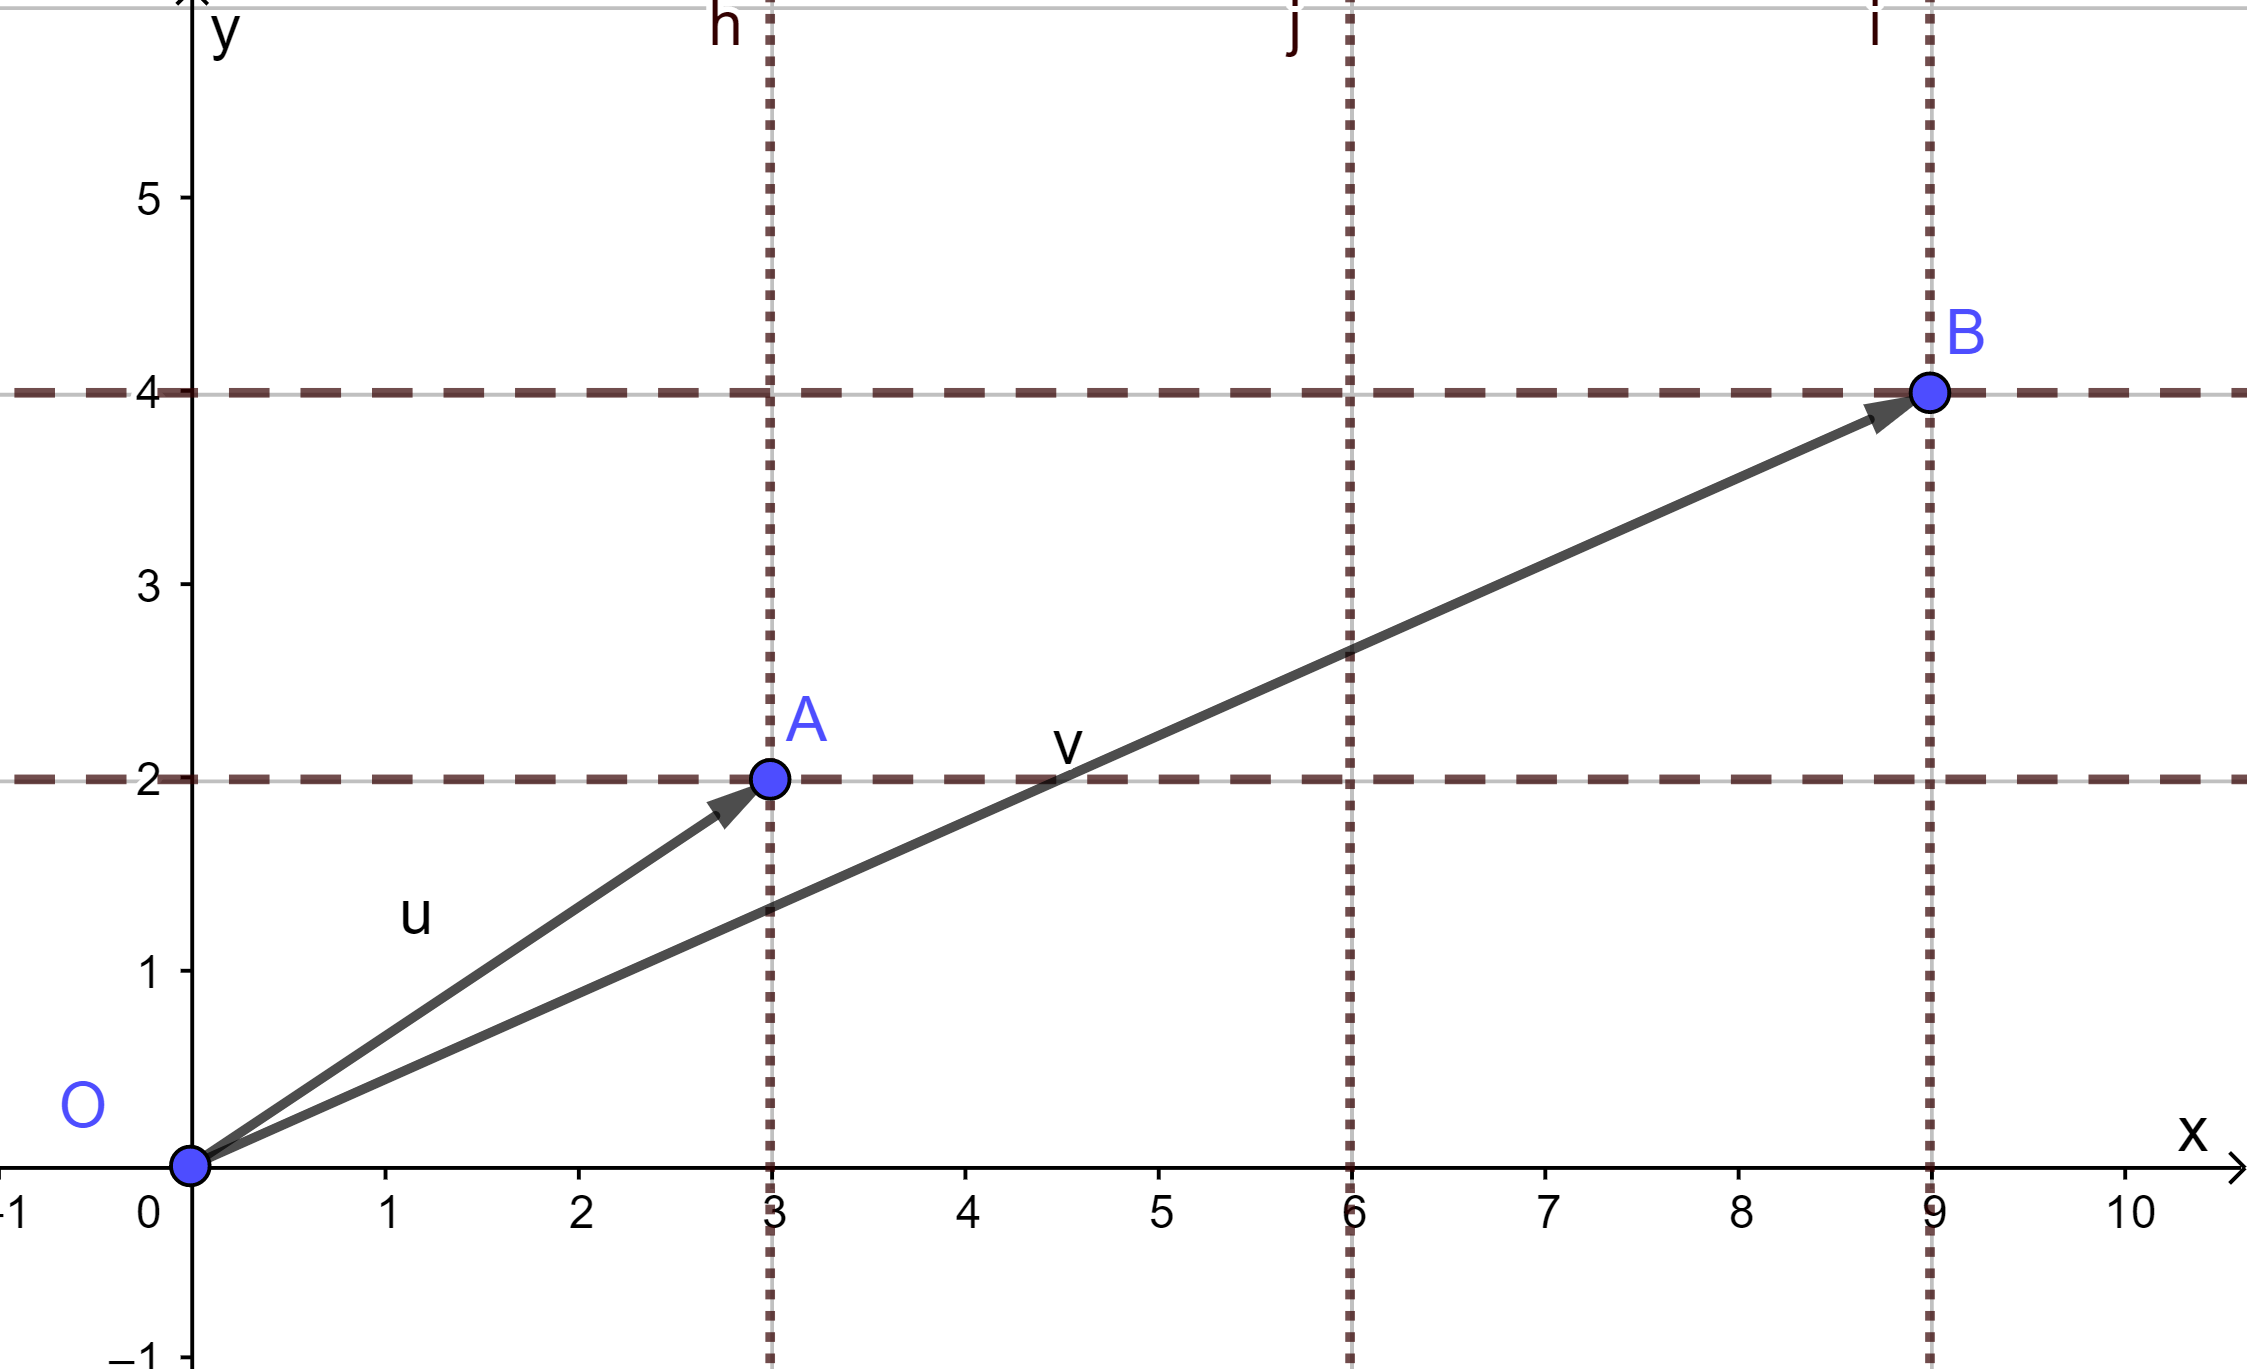
\includegraphics[width=\textwidth]{../Mathematik_1/Bilder/lineare_abbildungen_skalierung_ebene.png}
\end{minipage}
\begin{minipage}{0.5\textwidth}
\[
\begin{pmatrix}
x\\y
\end{pmatrix}
\mapsto
\begin{pmatrix}
3&0\\
0&2
\end{pmatrix}
\begin{pmatrix}
x\\y
\end{pmatrix}
=
\begin{pmatrix}
3x\\2y
\end{pmatrix}.
\]
\end{minipage}

\end{exabox}

\begin{exabox}{Drehung}{ }

\begin{minipage}{0.4\textwidth}
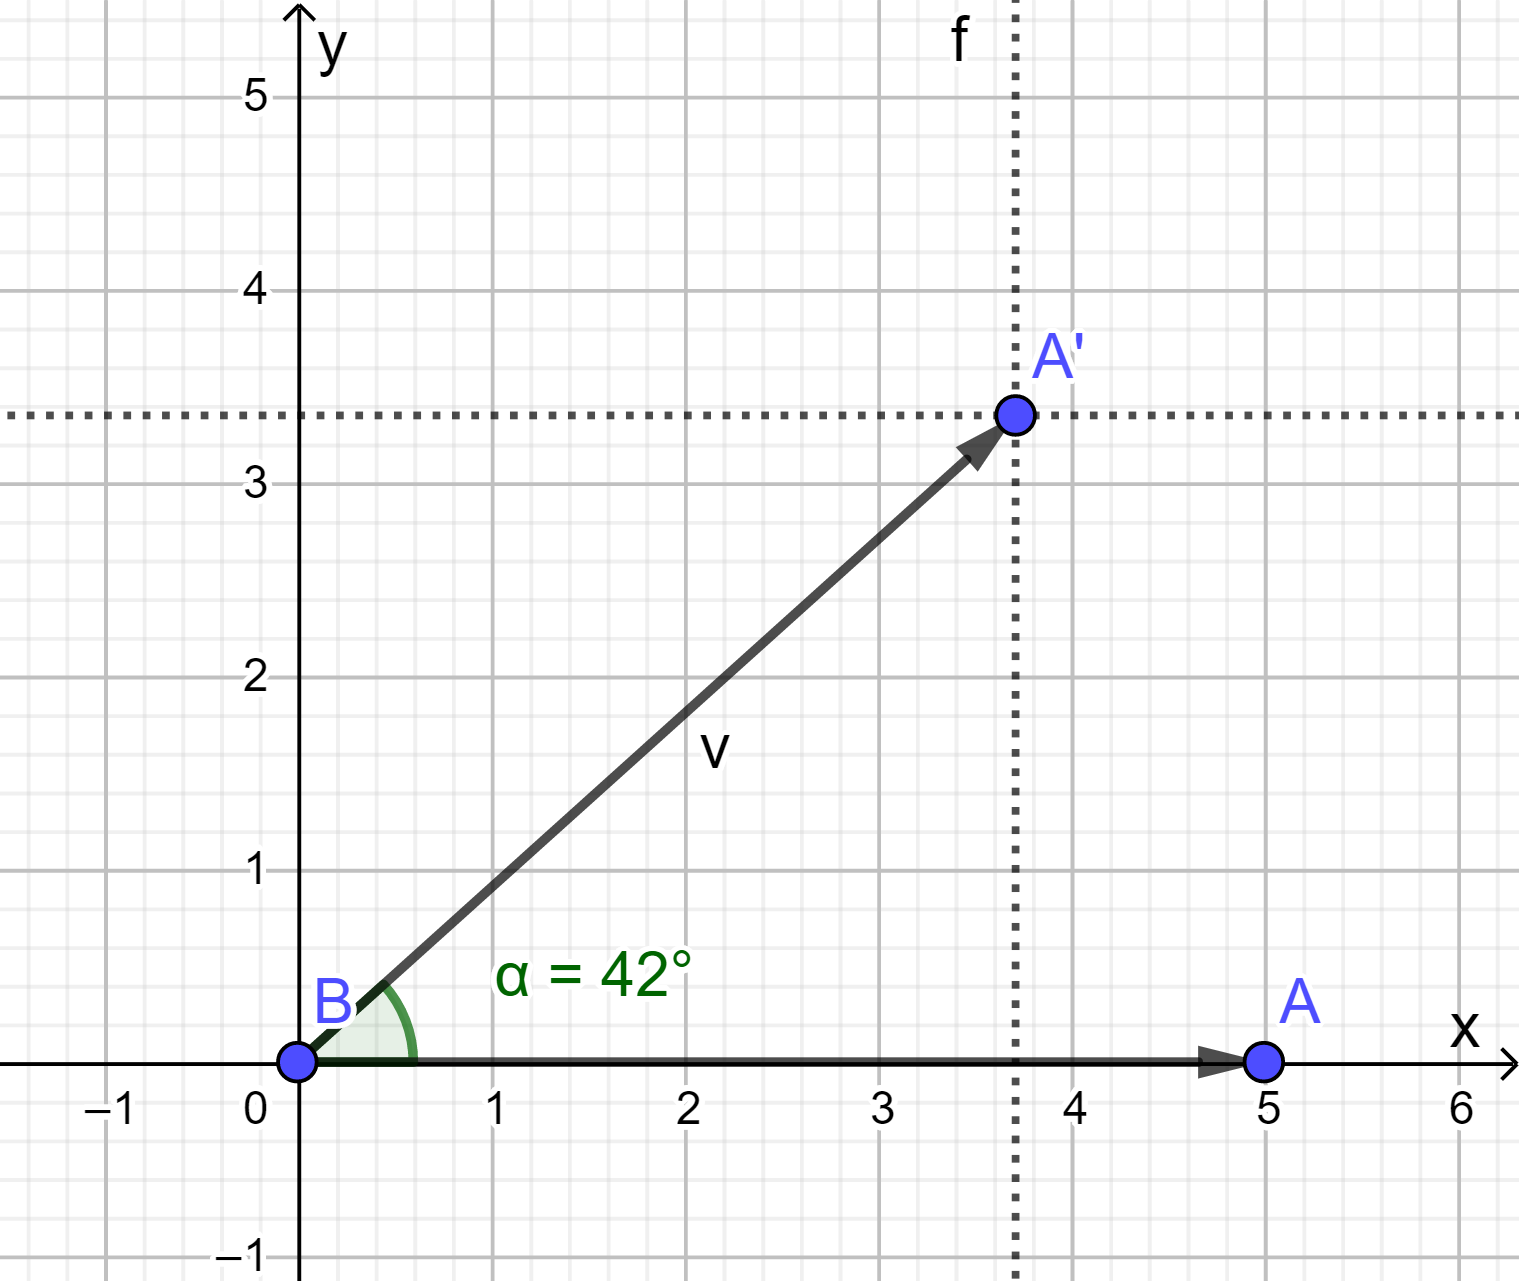
\includegraphics[width=\textwidth]{../Mathematik_1/Bilder/lineare_abbildungen_drehung_42_grad.png}
\end{minipage}
\begin{minipage}{0.55\textwidth}
\[
\begin{pmatrix}
x\\y
\end{pmatrix}
\mapsto
\underbrace{
\begin{pmatrix}
\cos\alpha&-\sin\alpha\\
\sin\alpha&\cos\alpha
\end{pmatrix}
}_{\textnormal{Drehmatrix}}
\begin{pmatrix}
x\\y
\end{pmatrix}.
\]
\end{minipage}

\end{exabox}

\noindent\textbf{Bemerkung:}
Eine Verschiebung um einen von Null verschiedenen Vektor ist keine lineare Abbildung. Jede lineare Abbildung erf�llt \(\mathcal A(\vec 0)=\vec 0\), w�hrend eine solche Verschiebung den Ursprung auf einen anderen Punkt abbildet.


\subsection{Matrix-Matrix-Multiplikation: Hintereinanderausf�hren}

Lineare Abbildungen k�nnen wie andere Funktionen miteinander verkettet werden. Sind
\[
\mathcal A:\mathbb K^n\to\mathbb K^p
\qquad\text{und}\qquad
\mathcal B:\mathbb K^p\to\mathbb K^m
\]
lineare Abbildungen, so ist auch ihre Komposition
\[
\mathcal B\circ\mathcal A:
\mathbb K^n\to\mathbb K^m
\]
linear.

Werden \(\mathcal A\) und \(\mathcal B\) durch die Matrizen \(A\) und \(B\) dargestellt, so gilt
\[
\mathcal B(\mathcal A(\vec x))
=
B(A\,\vec x)
=
(B\,A)\,\vec x.
\]

Die Matrixmultiplikation beschreibt damit das \textbf{Hintereinanderausf�hren linearer Abbildungen}.

\begin{defbox}{Matrix-Matrix-Multiplikation}{ }

F�r
\[
A\in\mathbb K^{m\times n},
\qquad
B\in\mathbb K^{n\times p}
\]
ist das Produkt
\[
	A\,B\in\mathbb K^{m\times p}
\]
durch
\[
	(A\,B)_{ij}
=
\sum_{k=1}^{n}a_{ik}b_{kj}
\]
definiert.

\end{defbox}

\begin{exabox}{Multiplikation}{ }

\[
\left(
\begin{array}{ccc}
\textcolor{brown}{1}&\textcolor{brown}{2}&\textcolor{brown}{3}\\
4&5&6
\end{array}
\right)
\left(
\begin{array}{cccc}
1&\textcolor{red}{0}&0&1\\
0&\textcolor{red}{3}&0&0\\
2&\textcolor{red}{4}&0&0
\end{array}
\right)
=
\left(
\begin{array}{cccc}
7&\textcolor{blue}{18}&0&1\\
16&39&0&4
\end{array}
\right),
\]
wobei beispielsweise
\[
(AB)_{\textcolor{blue}{12}}
=
\textcolor{brown}{1}\cdot\textcolor{red}{0}
+\textcolor{brown}{2}\cdot\textcolor{red}{3}
+\textcolor{brown}{3}\cdot\textcolor{red}{4}.
\]

\end{exabox}

\noindent\textbf{Bemerkung:}
Die Matrixmultiplikation ist assoziativ und distributiv, aber im Allgemeinen nicht kommutativ. Dies entspricht auch ihrer Interpretation als Hintereinanderausf�hren von Abbildungen: Die Reihenfolge der ausgef�hrten Transformationen kann das Ergebnis ver�ndern.

\begin{exabox}{Matrixmultiplikation ist im Allgemeinen nicht kommutativ}{ }

\[
{\color{brown}
\begin{pmatrix}
2&3\\4&5
\end{pmatrix}}
{\color{red}
\begin{pmatrix}
1&1\\0&1
\end{pmatrix}}
\neq
{\color{red}
\begin{pmatrix}
1&1\\0&1
\end{pmatrix}}
{\color{brown}
\begin{pmatrix}
2&3\\4&5
\end{pmatrix}}.
\]

\end{exabox}


\subsection{Bild und Rang: Welche Vektoren k�nnen herauskommen?}

Eine Matrix
\[
A\in\mathbb K^{m\times n}
\]
beschreibt eine lineare Abbildung von \(\mathbb K^n\) nach \(\mathbb K^m\). Dabei m�ssen jedoch nicht alle Vektoren der Zielmenge \(\mathbb K^m\) tats�chlich als Ergebnis der Abbildung auftreten.

Damit stellt sich die Frage, welche Vektoren durch die Abbildung �berhaupt erreicht werden k�nnen.

Die Menge aller Vektoren, die als \(A\vec x\) entstehen k�nnen, hei�t \textbf{Bild} (\emph{image}) der linearen Abbildung.

\begin{defbox}{Bild einer Matrix}{ }

F�r \(A\in\mathbb K^{m\times n}\) ist
\[
\operatorname{im}(A)
=
\left\{
\vec y\in\mathbb K^m:
\exists\,\vec x\in\mathbb K^n
\text{ mit }
\vec y=A\,\vec x
\right\}.
\]

\end{defbox}

Die zuvor betrachtete Spaltendarstellung liefert unmittelbar eine zweite Beschreibung des Bildes. Sind
\(\vec a_1,\ldots,\vec a_n\) die Spalten von \(A\), so gilt
\[
A\vec x
=
x_1\vec a_1+\cdots+x_n\vec a_n.
\]

Jeder Vektor im Bild ist daher eine Linearkombination der Spaltenvektoren.  Umgekehrt entsteht jede Linearkombination der Spalten durch eine geeignete Wahl der Komponenten von \(\vec x\). Damit gilt
\[
\operatorname{im}(A)
=
\operatorname{span}
\{\vec a_1,\ldots,\vec a_n\}.
\]

Das Bild einer Matrix ist somit ein Untervektorraum der Zielmenge \(\mathbb K^m\).

Die Dimension dieses Untervektorraums hei�t \textbf{Rang} (\emph{rank}) der Matrix.

\begin{defbox}{Rang einer Matrix}{ }

F�r \(A\in\mathbb K^{m\times n}\) ist
\[
\operatorname{rk}(A)
=
\dim\bigl(\operatorname{im}(A)\bigr).
\]

\end{defbox}

Der Rang beschreibt damit, wie viele voneinander unabh�ngige Richtungen im Bild der linearen Abbildung entstehen k�nnen. Wie der Rang einer konkreten Matrix systematisch bestimmt werden kann, wird im Zusammenhang mit linearen Gleichungssystemen untersucht.


\subsection{Kern und Defekt: Welche Vektoren verschwinden?}

Neben der Frage, welche Vektoren durch eine lineare Abbildung entstehen k�nnen, ist eine zweite Frage von grundlegender Bedeutung:

Welche Vektoren des Definitionsbereichs werden auf den Nullvektor \(\vec 0\) abgebildet?

Die Menge dieser Vektoren hei�t \textbf{Kern} (\emph{kernel}) der linearen Abbildung.

\begin{defbox}{Kern einer Matrix}{ }

F�r \(A\in\mathbb K^{m\times n}\) ist
\[
\ker(A)
=
\left\{
\vec x\in\mathbb K^n:
A\vec x=\vec 0
\right\}.
\]

\end{defbox}

Der Kern ist ein \underline{Untervektorraum}\randverweis{MA1-vektorraum} des Definitionsbereichs \(\mathbb K^n\). Enth�lt der Kern au�er dem Nullvektor weitere Vektoren, so werden verschiedene Vektoren durch die Abbildung auf denselben Vektor abgebildet. Denn aus
\[
	A\, \vec v=\vec0
\]
folgt f�r jeden Vektor \(\vec x\)
\[
	A\,(\vec x+\vec v) = A\,\vec x+A\,\vec v = A\vec x.
\]

Die Dimension des Kerns hei�t \textbf{Defekt} der Matrix.

\begin{defbox}{Defekt einer Matrix}{ }

F�r \(A\in\mathbb K^{m\times n}\) ist
\[
\operatorname{def}(A)
=
\dim\bigl(\ker(A)\bigr).
\]

\end{defbox}

Bild und Kern beschreiben damit zwei unterschiedliche Aspekte derselben linearen Abbildung: Das Bild beschreibt, welche Richtungen durch die Abbildung erreicht werden, w�hrend der Kern beschreibt, welche Richtungen bei der Abbildung auf den Nullvektor abgebildet werden.

Zwischen den Dimensionen dieser beiden Unterr�ume besteht ein grundlegender Zusammenhang.

\begin{theorembox}{Rangsatz}{ }

F�r \(A\in\mathbb K^{m\times n}\) gilt
\[
\operatorname{rk}(A)+\operatorname{def}(A)=n.
\]

\end{theorembox}

Der Rangsatz zerlegt die Dimension des Definitionsbereichs in zwei Anteile: die Dimension des Bildes und die Dimension des Kerns. Wie diese Gr��en f�r konkrete Matrizen bestimmt werden k�nnen, f�hrt unmittelbar zu den Methoden f�r lineare Gleichungssysteme.

  % Matrizen % GEOGEBRA APPS
\newpage
\setcounter{satz}{0} \setcounter{def}{0} \setcounter{exa}{0}  \section{Lineare Gleichungssysteme}\label{MA1-lineare-gleichungssysteme}

\begin{table}[H]
  \centering
  \begin{tabularx}{\textwidth}{p{0.9\textwidth} p{0.1\textwidth}}
    \toprule
    \multicolumn{2}{c}{\textbf{�bersicht �ber Lernziele und Voraussetzungen}}\\
    \midrule
    \textbf{Lernziele} &\\[.5\normalbaselineskip]
    \tabitem lineare Gleichungssysteme in Gleichungs-, Vektor- und Matrixform darstellen &\\
    \tabitem lineare Gleichungssysteme mit dem Gau�schen Eliminationsverfahren systematisch l�sen &\\
    \tabitem die L�sbarkeit und Eindeutigkeit eines linearen Gleichungssystems mithilfe von Rang und Kern untersuchen &\\
    \tabitem die Struktur der L�sungsmenge eines linearen Gleichungssystems bestimmen und interpretieren &\\
    \tabitem Rang, Kern und Defekt einer Matrix mithilfe des Gau�schen Eliminationsverfahrens bestimmen &\\
    \tabitem die lineare Unabh�ngigkeit beziehungsweise Abh�ngigkeit gegebener Vektoren systematisch untersuchen &\\
    \midrule
    \textbf{Voraussetzungen} &\\[.5\normalbaselineskip]
    \tabitem Vektoren & \abschnittsverweis{MA1-vektoren}\\
    \tabitem Vektorr�ume, Linearkombinationen und lineare Unabh�ngigkeit & \abschnittsverweis{MA1-vektorraum}\\
    \tabitem Matrizen, lineare Abbildungen, Bild, Rang, Kern und Defekt & \abschnittsverweis{MA1-matrizen}\\
    \bottomrule
  \end{tabularx}
\end{table}

\ifintegriereaufgaben
\noindent �bungsaufgaben zum Thema finden sich hier:
\hyperref[MA1-lineare-gleichungssysteme-aufgaben]{Aufgaben}
\vspace{0.3cm}
\hrule
\fi


%----------------------------------------------------------
\subsection{Was ist ein lineares Gleichungssystem?}

Ein \textbf{lineares Gleichungssystem} (\emph{system of linear equations}) besteht aus mehreren linearen Gleichungen, die gleichzeitig erf�llt sein sollen. Die gesuchten Gr��en treten dabei nur in erster Potenz und jeweils mit konstanten Koeffizienten auf.

Ein Beispiel mit drei Gleichungen und vier Unbekannten ist
\[
(*)\qquad
\left\{
\begin{array}{rcrcrcrcl}
23x &+&45y&-&3z&+&4w&=&7,\\
    &&2y&-&z&+&6w&=&-3,\\
-15x&+&5y&&&-&3w&=&5.
\end{array}
\right.
\]

Eine L�sung des Gleichungssystems ist ein Vektor
\[
\begin{pmatrix}x&y&z&w\end{pmatrix}^{\intercal}\in\mathbb R^4,
\]
dessen Komponenten alle drei Gleichungen gleichzeitig erf�llen. Die L�sungsmenge \(\mathbb L\) ist daher eine Teilmenge von \(\mathbb R^4\).  Es ist zun�chst nicht klar, ob diese Menge �berhaupt Elemente enth�lt und, falls dies der Fall ist, ob sie aus einem einzigen oder aus mehreren Vektoren besteht.

Die Linearit�t der Gleichungen zeigt sich darin, dass ausschlie�lich konstante Vielfache der Unbekannten addiert werden. Terme wie \(\sin(x)\), \(y^2\) oder \(xz\) w�rden zu nichtlinearen Gleichungen f�hren.

Das Gleichungssystem kann zun�chst als Vektorgleichung gelesen werden.  Werden die Koeffizienten jeder Unbekannten zu einem Vektor zusammengefasst, so entsteht
\[
(*)\quad\Longleftrightarrow\quad
x
\begin{pmatrix}
23\\0\\-15
\end{pmatrix}
+
y
\begin{pmatrix}
45\\2\\5
\end{pmatrix}
+
z
\begin{pmatrix}
-3\\-1\\0
\end{pmatrix}
+
w
\begin{pmatrix}
4\\6\\-3
\end{pmatrix}
=
\begin{pmatrix}
7\\-3\\5
\end{pmatrix}.
\]

Damit erh�lt das L�sen des Gleichungssystems eine bereits bekannte Bedeutung: Gesucht sind Koeffizienten \(x,y,z,w\), mit denen sich der Vektor auf der rechten Seite als Linearkombination der vier Vektoren auf der linken Seite darstellen l�sst.

Werden diese vier Vektoren als Spalten einer Matrix angeordnet, entsteht schlie�lich die Matrixform des Gleichungssystems.

\begin{exabox}{Lineares Gleichungssystem in Matrixform}{ }

\[
(*)\quad\Longleftrightarrow\quad
\underbrace{
\begin{pmatrix}
23&45&-3&4\\
0&2&-1&6\\
-15&5&0&-3
\end{pmatrix}}_{\displaystyle A}
\underbrace{
\begin{pmatrix}
x\\y\\z\\w
\end{pmatrix}}_{\displaystyle\vec x}
=
\underbrace{
\begin{pmatrix}
7\\-3\\5
\end{pmatrix}}_{\displaystyle\vec b}.
\]

Kurz geschrieben lautet das Gleichungssystem damit
\[
A\vec x=\vec b.
\]

\end{exabox}

Die drei Schreibweisen beschreiben dasselbe mathematische Problem. Sie heben jedoch unterschiedliche Aspekte hervor: Die Gleichungsform zeigt die einzelnen Bedingungen, die Vektorform zeigt die gesuchte Linearkombination und die Matrixform erm�glicht eine systematische algebraische Bearbeitung.

Die zuvor eingef�hrten Begriffe\wennreferenzvorhanden{MA1-vektoren}{\wennreferenzvorhanden{MA1-matrizen}{ (Abschnitte \abschnittsverweis{MA1-vektoren}--\abschnittsverweis{MA1-matrizen})}} erm�glichen bereits eine strukturelle Beschreibung dieses Problems. F�r
\[
A\vec x=\vec b
\]
stellen sich insbesondere die Fragen, ob \(\vec b\) im Bild von \(A\) liegt und ob der Kern von \(A\) au�er dem Nullvektor weitere Vektoren enth�lt.  Damit h�ngen Existenz und Eindeutigkeit einer L�sung unmittelbar mit Bild, Rang, Kern und Defekt der Matrix zusammen.

Bisher wurden diese Begriffe vor allem inhaltlich beschrieben. Nun kommt eine systematische Rechenmethode hinzu. Das Gau�sche Eliminationsverfahren erm�glicht nicht nur das L�sen linearer Gleichungssysteme. Mit derselben Grundidee lassen sich auch Rang und Kern einer Matrix bestimmen und Fragen nach linearer Abh�ngigkeit, Erzeugendensystemen und Basen rechnerisch untersuchen.

Lineare Gleichungssysteme bilden damit den konkreten Ausgangspunkt f�r eine Rechenmethode, mit der sich mehrere der zuvor eingef�hrten Begriffe der linearen Algebra praktisch untersuchen lassen.


%----------------------------------------------------------
\subsection{Existenz und Eindeutigkeit von L�sungen}

Bevor konkrete Gleichungssysteme gel�st werden, lassen sich die Fragen nach Existenz und Eindeutigkeit bereits mithilfe von Bild und Kern einer Matrix beschreiben.

Es sei
\[
A\in\mathbb R^{m\times n},
\qquad
\vec x\in\mathbb R^n,
\qquad
\vec b\in\mathbb R^m.
\]
Das lineare Gleichungssystem
\[
A\vec x=\vec b
\]
ist genau dann l�sbar, wenn es einen Vektor \(\vec x\) gibt, der durch \(A\) auf \(\vec b\) abgebildet wird.

Nach der Definition des Bildes bedeutet dies gerade, dass \(\vec b\) im Bild von \(A\) liegen muss.

\begin{theorembox}{Bedingung f�r die L�sbarkeit eines linearen Gleichungssystems}{ }

Das lineare Gleichungssystem
\[
A\vec x=\vec b
\]
besitzt mindestens eine L�sung genau dann, wenn
\[
\vec b\in\operatorname{im}(A).
\]

\end{theorembox}

Damit beantwortet der Begriff des Bildes die Frage nach der \textbf{Existenz} einer L�sung.

Nach der Existenz stellt sich die Frage nach der Eindeutigkeit. Angenommen, \(\vec x_1\) und \(\vec x_2\) seien zwei L�sungen desselben Gleichungssystems. Dann gilt
\[
A\vec x_1=A\vec x_2=\vec b.
\]
Durch Subtraktion folgt
\[
A(\vec x_1-\vec x_2)=\vec0.
\]

Die Differenz zweier L�sungen liegt also im Kern von \(A\).

Ein Gleichungssystem mit rechter Seite \(\vec0\),
\[
A\vec x=\vec0,
\]
hei�t \textbf{homogenes lineares Gleichungssystem} (\emph{homogeneous system of linear equations}). Ein Gleichungssystem mit einer von Null verschiedenen rechten Seite wird entsprechend \textbf{inhomogen} genannt.

Besitzt das homogene Gleichungssystem nur die triviale L�sung \(\vec x=\vec0\), so kann die Differenz zweier L�sungen nur der Nullvektor sein. In diesem Fall m�ssen zwei m�gliche L�sungen identisch sein.

Besitzt das homogene Gleichungssystem dagegen eine nichttriviale L�sung \(\vec v\neq\vec0\), so gilt
\[
A\vec v=\vec0.
\]
Ist \(\vec x_s\) eine L�sung von \(A\vec x=\vec b\), dann ist auch
\[
A(\vec x_s+\vec v)
=
A\vec x_s+A\vec v
=
\vec b.
\]
Eine vorhandene L�sung kann dann also nicht eindeutig sein.

\begin{theorembox}{Bedingung f�r die Eindeutigkeit einer L�sung}{ }

Das lineare Gleichungssystem
\[
A\vec x=\vec b
\]
besitzt h�chstens eine L�sung genau dann, wenn
\[
\ker(A)=\{\vec0\}.
\]

Besitzt das Gleichungssystem zus�tzlich mindestens eine L�sung, so ist diese L�sung eindeutig.

\end{theorembox}

Damit beantworten zwei der Begriffe aus dem vorangegangenen Abschnitt die beiden grundlegenden Fragen:
\[
\vec b\in\operatorname{im}(A)
\quad\Longleftrightarrow\quad
\text{Existenz einer L�sung},
\]
w�hrend
\[
\ker(A)=\{\vec0\}
\quad\Longleftrightarrow\quad
\text{h�chstens eine L�sung}
\]
gilt.

F�r eine eindeutig bestimmte L�sung m�ssen beide Bedingungen gleichzeitig erf�llt sein.


%----------------------------------------------------------
\subsection{Das Gau�sche Eliminationsverfahren}

Die bisherigen �berlegungen beschreiben, welche Bedingungen �ber L�sbarkeit und Eindeutigkeit entscheiden. F�r eine konkrete Matrix fehlt jedoch noch ein systematisches Verfahren, mit dem diese Bedingungen �berpr�ft und die L�sungen tats�chlich bestimmt werden k�nnen.

Dazu sei ein allgemeines lineares Gleichungssystem
\[
\begin{pmatrix}
a_{11}&\cdots&a_{1n}\\
\vdots&\ddots&\vdots\\
a_{m1}&\cdots&a_{mn}
\end{pmatrix}
\begin{pmatrix}
x_1\\
\vdots\\
x_n
\end{pmatrix}
=
\begin{pmatrix}
b_1\\
\vdots\\
b_m
\end{pmatrix}
\]
mit
\[
A\in\mathbb R^{m\times n},
\qquad
\vec x\in\mathbb R^n,
\qquad
\vec b\in\mathbb R^m
\]
gegeben.

Je nach Anzahl der Gleichungen und Unbekannten hei�t das Gleichungssystem

\begin{itemize}
  \item \textbf{unterbestimmt}, wenn es mehr Unbekannte als Gleichungen gibt,
  also \(n>m\),
  \item \textbf{quadratisch}, wenn es ebenso viele Unbekannte wie Gleichungen
  gibt, also \(n=m\),
  \item \textbf{�berbestimmt}, wenn es mehr Gleichungen als Unbekannte gibt,
  also \(m>n\).
\end{itemize}

Allein aus dieser Einteilung l�sst sich im Allgemeinen noch nicht entscheiden, ob ein konkretes Gleichungssystem l�sbar ist. Daf�r m�ssen die Gleichungen selbst untersucht werden.

Das grundlegende Verfahren daf�r ist das \textbf{Gau�sche Eliminationsverfahren} (\emph{Gaussian elimination}).  Seine Idee besteht darin, ein Gleichungssystem durch �quivalenzumformungen schrittweise in eine Form zu �berf�hren, aus der sich die L�sungen und weitere Eigenschaften des Systems leichter ablesen lassen.


%----------------------------------------------------------
\subsubsection*{Elementare Zeilenumformungen}

Bereits bei einzelnen Gleichungen wurden �quivalenzumformungen verwendet: Eine Gleichung wird ver�ndert, ohne ihre L�sungsmenge zu ver�ndern. Beim Gau�schen Eliminationsverfahren wird dieselbe Idee auf ein ganzes Gleichungssystem �bertragen.

Dabei sind drei grundlegende Umformungen zul�ssig:

\begin{enumerate}
  \item Zwei Gleichungen k�nnen miteinander vertauscht werden.
  \item Eine Gleichung kann mit einem von Null verschiedenen Skalar multipliziert werden.
  \item Zu einer Gleichung kann ein Vielfaches einer anderen Gleichung
  addiert werden.
\end{enumerate}

Diese Operationen ver�ndern die L�sungsmenge des Gleichungssystems nicht.  In Matrixdarstellung entsprechen sie den \textbf{elementaren Zeilenumformungen} (\emph{elementary row operations}).

Da beim L�sen eines inhomogenen Gleichungssystems auch die rechte Seite von jeder Umformung betroffen ist, werden Koeffizientenmatrix und rechte Seite gemeinsam in der \textbf{erweiterten Matrix} (\emph{augmented matrix}) zusammengefasst:

\[
A\vec x=\vec b
\qquad\longrightarrow\qquad
A_{\vec b}:=
\left(
\begin{array}{ccc|c}
a_{11}&\cdots&a_{1n}&b_1\\
\vdots&\ddots&\vdots&\vdots\\
a_{m1}&\cdots&a_{mn}&b_m
\end{array}
\right).
\]

Jede Zeile dieser erweiterten Matrix steht weiterhin f�r eine Gleichung des urspr�nglichen Gleichungssystems.


%----------------------------------------------------------
\subsubsection*{Zeilenstufenform}

Ziel des Gau�schen Eliminationsverfahrens ist es zun�chst, durch elementare Zeilenumformungen unterhalb geeigneter f�hrender Eintr�ge Nullen zu erzeugen.  Dadurch entsteht schrittweise eine \textbf{Zeilenstufenform} (\emph{row echelon form}), die auch als Trapezform bezeichnet wird.

In einer Zeilenstufenform liegen die f�hrenden von Null verschiedenen Eintr�ge aufeinanderfolgender Zeilen jeweils weiter rechts. Vollst�ndig aus Nullen bestehende Zeilen stehen am unteren Ende der Matrix.  

Das L�sen erfolgt damit in zwei Schritten:

\begin{enumerate}
  \item Die erweiterte Matrix \(A_{\vec b}\) wird durch elementare Zeilenumformungen in Zeilenstufenform gebracht.
  \item Anschlie�end werden die zugeh�rigen Gleichungen von unten nach oben aufgel�st.
\end{enumerate}

Die Zeilenstufenform liefert jedoch mehr als nur einen bequemeren Weg zur L�sung. An ihr werden auch Rang, freie Unbekannte und m�gliche Widerspr�che sichtbar. Dadurch verbindet das Gau�sche Eliminationsverfahren das eigentliche L�sen mit den zuvor eingef�hrten strukturellen Begriffen.


%----------------------------------------------------------
\subsubsection*{L�sbarkeit und Eindeutigkeit aus dem Rang}

Die erweiterte Matrix erlaubt es, die Frage
\[
\vec b\in\operatorname{im}(A)
\]
rechnerisch zu untersuchen.

Die Spalten von \(A\) spannen das Bild von \(A\) auf. Wird die rechte Seite \(\vec b\) als zus�tzliche Spalte erg�nzt, gibt es zwei M�glichkeiten: Entweder liegt \(\vec b\) bereits im von den Spalten von \(A\) aufgespannten Raum, oder durch die zus�tzliche Spalte entsteht eine weitere unabh�ngige Richtung.

Im ersten Fall ver�ndert sich der Rang nicht. Im zweiten Fall erh�ht sich der Rang durch das Hinzuf�gen von \(\vec b\). Genau dann kann \(\vec b\) nicht als Linearkombination der Spalten von \(A\) dargestellt werden und das Gleichungssystem besitzt keine L�sung.

\begin{theorembox}{L�sbarkeit und Eindeutigkeit aus dem Rang}{ }

Es sei
\[
A\in\mathbb R^{m\times n}.
\]
Dann gilt:

\begin{itemize}
  \item
  \(\operatorname{rk}(A)\neq\operatorname{rk}(A_{\vec b})\)

  \(\Rightarrow\) Das Gleichungssystem ist nicht l�sbar.

  \item
  \(\operatorname{rk}(A)=\operatorname{rk}(A_{\vec b})<n\)

  \(\Rightarrow\) Das Gleichungssystem besitzt unendlich viele L�sungen.

  \item
  \(\operatorname{rk}(A)=\operatorname{rk}(A_{\vec b})=n\)

  \(\Rightarrow\) Das Gleichungssystem besitzt genau eine L�sung.
\end{itemize}

\end{theorembox}

Damit werden die abstrakten Bedingungen �ber Bild und Kern durch ein konkretes Rechenverfahren zug�nglich.


%----------------------------------------------------------
\subsection{Beispiele zum Gau�schen Eliminationsverfahren}

Die verschiedenen M�glichkeiten f�r die L�sungsmenge werden nun an konkreten Gleichungssystemen sichtbar.


%----------------------------------------------------------
\begin{exabox}{Beispiel \(1\): \(\operatorname{rk}(A)\neq\operatorname{rk}(A_{\vec b})\)}{ }

Es ist \(A\in\mathbb R^{2\times2}\) beziehungsweise \(A_{\vec b}\in\mathbb R^{2\times3}\) mit
\[
A_{\vec b}
=
\left(
\begin{array}{cc|c}
1&3&5\\
2&6&7
\end{array}
\right).
\]

Durch �quivalente Zeilenumformungen entsteht die Zeilenstufenform
\[
\left(
\begin{array}{cc|c}
1&3&5\\
0&0&-3
\end{array}
\right).
\]

Die zweite Zeile entspricht der Gleichung
\[
0=-3.
\]
Damit ist unmittelbar ein Widerspruch entstanden. Das Gleichungssystem ist also nicht l�sbar.

Dies l�sst sich zugleich �ber die R�nge ausdr�cken:
\[
\operatorname{rk}(A)=1
\neq
\operatorname{rk}(A_{\vec b})=2.
\]

Die zus�tzliche Spalte \(\vec b\) erh�ht den Rang. Der Vektor \(\vec b\) liegt daher nicht im Bild von \(A\), und die L�sungsmenge ist
\[
\mathbb L=\emptyset.
\]

\end{exabox}


%----------------------------------------------------------
\begin{exabox}{Beispiel \(2\): \(\operatorname{rk}(A)=\operatorname{rk}(A_{\vec b})<n\)}{ }

Es ist \(A\in\mathbb R^{3\times4}\) beziehungsweise \(A_{\vec b}\in\mathbb R^{3\times5}\) mit
\[
A_{\vec b}
=
\left(
\begin{array}{rrrr|r}
1&0&0&1&0\\
0&1&0&1&1\\
2&0&1&0&-4
\end{array}
\right).
\]

Durch �quivalente Zeilenumformungen entsteht die Zeilenstufenform
\[
\left(
\begin{array}{rrrr|r}
1&0&0&1&0\\
0&1&0&1&1\\
0&0&1&-2&-4
\end{array}
\right).
\]

Damit gilt
\[
\operatorname{rk}(A)
=
\operatorname{rk}(A_{\vec b})
=
3<n=4.
\]

Das Gleichungssystem ist also l�sbar, aber die L�sung ist nicht eindeutig.  Da vier Unbekannte vorhanden sind, aber nur drei f�hrende Unbekannte auftreten, bleibt eine Unbekannte frei.

F�r \(x_4\) kann daher ein Parameter
\[
x_4=\alpha\in\mathbb R
\]
gew�hlt werden. Die �brigen Gleichungen werden von unten nach oben aufgel�st:
\[
\begin{cases}
x_4 &= \alpha,\\
x_3 &= -4+2x_4
      \Rightarrow x_3=-4+2\alpha,\\
x_2 &= 1-x_4
      \Rightarrow x_2=1-\alpha,\\
x_1 &= -x_4
      \Rightarrow x_1=-\alpha.
\end{cases}
\]

Damit ergibt sich
\[
\vec x
=
\begin{pmatrix}
-\alpha\\
-4+2\alpha\\
1-\alpha\\
\alpha
\end{pmatrix}
=
\underbrace{
\begin{pmatrix}
0\\
-4\\
1\\
0
\end{pmatrix}}_{\displaystyle\vec x_s}
+
\alpha
\underbrace{
\begin{pmatrix}
-1\\
2\\
-1\\
1
\end{pmatrix}}_{\displaystyle\vec x_h}.
\]

Dabei gilt
\[
A\vec x_s=\vec b
\]
und
\[
A\vec x_h=\vec0.
\]

Der Vektor \(\vec x_s\) ist also eine spezielle L�sung des inhomogenen Gleichungssystems. Der Vektor \(\vec x_h\) ist eine nichttriviale L�sung des zugeh�rigen homogenen Gleichungssystems und liegt damit im Kern von \(A\).  

Da in diesem Beispiel nur ein freier Parameter auftritt, gilt sogar
\[
\ker(A)
=
\operatorname{span}\{\vec x_h\}.
\]

\medskip
\noindent\textbf{Erkenntnis:}

Die gesamte L�sungsmenge entsteht aus einer speziellen L�sung und allen Vektoren des Kerns:
\[
\mathbb L
=
\vec x_s+\ker(A)
=
\left\{
\vec x_s+\vec x_h:
\vec x_h\in\ker(A)
\right\}.
\]

In diesem Beispiel besitzt der Kern die Dimension \(1\). Daher gilt
\[
\operatorname{def}(A)=1.
\]

\end{exabox}


%----------------------------------------------------------
\begin{exabox}{Beispiel \(3\): quadratisches Gleichungssystem mit nicht eindeutiger L�sung}{ }

Es ist \(A\in\mathbb R^{4\times4}\) beziehungsweise
\(A_{\vec b}\in\mathbb R^{4\times5}\) mit
\[
A_{\vec b}
=
\left(
\begin{array}{rrrr|r}
1&2&-1&1&1\\
1&4&3&1&3\\
-1&-1&3&2&6\\
3&6&-3&4&5
\end{array}
\right)
\Longleftrightarrow
\left(
\begin{array}{rrrr|r}
1&2&-1&1&1\\
0&1&2&0&1\\
0&0&0&1&2\\
0&0&0&0&0
\end{array}
\right).
\]

Aus der Zeilenstufenform folgt
\[
\operatorname{rk}(A)
=
\operatorname{rk}(A_{\vec b})
=
3<n=4.
\]

Das Gleichungssystem ist damit l�sbar, aber nicht eindeutig. Obwohl das urspr�ngliche Gleichungssystem ebenso viele Gleichungen wie Unbekannte besitzt, sind nicht alle vier Gleichungen voneinander unabh�ngig. Der Rang betr�gt nur \(3\).

Die Variable \(x_3\) kann frei gew�hlt werden:
\[
x_3=\alpha\in\mathbb R.
\]
Von unten nach oben folgt
\[
\begin{cases}
x_4 &= 2,\\
x_3 &= \alpha,\\
x_2 &= 1-2x_3
      \Rightarrow x_2=1-2\alpha,\\
x_1 &= 1-2x_2+x_3-x_4
      \Rightarrow x_1=-3+5\alpha.
\end{cases}
\]

Damit ergibt sich
\[
\vec x
=
\begin{pmatrix}
-3+5\alpha\\
1-2\alpha\\
\alpha\\
2
\end{pmatrix}
=
\underbrace{
\begin{pmatrix}
-3\\
1\\
0\\
2
\end{pmatrix}}_{\displaystyle\vec x_s}
+
\alpha
\underbrace{
\begin{pmatrix}
5\\
-2\\
1\\
0
\end{pmatrix}}_{\displaystyle\vec x_h}.
\]

Wieder gilt
\[
A\vec x_s=\vec b,
\qquad
A\vec x_h=\vec0.
\]

Damit ist
\[
\ker(A)
=
\operatorname{span}
\left\{
\begin{pmatrix}
5\\-2\\1\\0
\end{pmatrix}
\right\}
\]
und
\[
\operatorname{def}(A)=1.
\]

\medskip
\noindent\textbf{Erkenntnis:}

Auch ein quadratisches Gleichungssystem muss nicht eindeutig l�sbar sein.  Entscheidend ist nicht allein die Anzahl der Gleichungen und Unbekannten, sondern der Rang der Koeffizientenmatrix.

Ist der Kern nicht trivial, so besitzt ein l�sbares Gleichungssystem mehrere L�sungen. Allgemein gilt wiederum
\[
\mathbb L=\vec x_s+\ker(A).
\]

\end{exabox}


%----------------------------------------------------------
\begin{exabox}{Beispiel \(4\): eindeutig l�sbares quadratisches Gleichungssystem}{ }

Es ist \(A\in\mathbb R^{4\times4}\) beziehungsweise \(A_{\vec b}\in\mathbb R^{4\times5}\) mit
\[
A_{\vec b}
=
\left(
\begin{array}{rrrr|r}
2&4&0&4&8\\
1&3&1&4&10\\
-2&-2&1&1&7\\
0&-1&0&1&-1
\end{array}
\right)
\Longleftrightarrow
\left(
\begin{array}{rrrr|r}
2&4&0&4&8\\
0&-2&-2&-4&-12\\
0&0&-1&1&3\\
0&0&0&8&16
\end{array}
\right).
\]

In jeder der vier Spalten der Koeffizientenmatrix befindet sich eine Pivotposition. Daher gilt
\[
\operatorname{rk}(A)
=
\operatorname{rk}(A_{\vec b})
=
4=n.
\]

Damit ist das Gleichungssystem eindeutig l�sbar. Gleichzeitig folgt aus dem Rangsatz
\[
\operatorname{def}(A)
=
n-\operatorname{rk}(A)
=
4-4
=
0,
\]
also
\[
\ker(A)=\{\vec0\}.
\]

Die L�sung wird von unten nach oben bestimmt:
\[
\begin{cases}
8x_4 &=16
       \Rightarrow x_4=2,\\
-x_3 &=3-x_4=3-2
       \Rightarrow x_3=-1,\\
-2x_2 &=-12+2x_3+4x_4
       =-12-2+8
       \Rightarrow x_2=3,\\
2x_1 &=8-4x_2-4x_4
       =8-12-8
       \Rightarrow x_1=-6.
\end{cases}
\]

Damit lautet die eindeutig bestimmte L�sung
\[
\vec x
=
\begin{pmatrix}
-6\\
3\\
-1\\
2
\end{pmatrix}.
\]

\medskip
\noindent\textbf{Erkenntnis:}

In diesem Beispiel ist \(A\) quadratisch und besitzt vollen Rang:
\[
\operatorname{rk}(A)=4.
\]
Damit gilt sowohl
\[
\ker(A)=\{\vec0\}
\]
als auch
\[
\operatorname{im}(A)=\mathbb R^4.
\]

Das bedeutet: F�r jede rechte Seite \(\vec b\in\mathbb R^4\) besitzt das Gleichungssystem \(A\vec x=\vec b\) genau eine L�sung.

Diese besondere Eigenschaft quadratischer Matrizen f�hrt im folgenden Abschnitt zum Begriff der inversen Matrix.

\end{exabox}


%----------------------------------------------------------
\begin{exabox}{Beispiel \(5\): �berbestimmtes, nicht l�sbares Gleichungssystem}{ }

Es ist \(A\in\mathbb R^{4\times3}\) beziehungsweise \(A_{\vec b}\in\mathbb R^{4\times4}\) mit
\[
A_{\vec b}
=
\left(
\begin{array}{rrr|r}
1&-1&1&0\\
3&2&1&2\\
1&2&4&0\\
-1&7&1&2
\end{array}
\right)
\Longleftrightarrow
\left(
\begin{array}{rrr|r}
1&-1&1&0\\
0&5&-2&2\\
0&0&-7&2\\
0&0&-11&1
\end{array}
\right).
\]

Die letzten beiden Zeilen enthalten Bedingungen an dieselbe verbleibende Unbekannte, die nicht gleichzeitig erf�llt werden k�nnen. Durch eine weitere Zeilenumformung entsteht entsprechend eine Widerspruchszeile.

Dies zeigt sich auch an den R�ngen:
\[
\operatorname{rk}(A)=3
\neq
\operatorname{rk}(A_{\vec b})=4.
\]

Die rechte Seite \(\vec b\) liegt also nicht im Bild von \(A\). F�r die gegebene rechte Seite ist das Gleichungssystem nicht l�sbar und
\[
\mathbb L=\emptyset.
\]

\medskip
\noindent\textbf{Erkenntnis:}

Bei einem �berbestimmten Gleichungssystem mit \(m>n\) gibt es mehr Gleichungen als Unbekannte. Ob eine L�sung existiert, h�ngt davon ab, ob die rechte Seite mit allen Bedingungen vertr�glich ist.

�berbestimmt bedeutet daher nicht automatisch unl�sbar. Entscheidend bleibt die Bedingung
\[
\operatorname{rk}(A)=\operatorname{rk}(A_{\vec b}).
\]

\end{exabox}


\subsection{Das Gau�verfahren als Werkzeug der linearen Algebra}

Das Gau�sche Eliminationsverfahren wurde ausgehend von linearen
Gleichungssystemen entwickelt. Mit derselben Systematik lassen sich jedoch
auch mehrere der zuvor eingef�hrten Begriffe der linearen Algebra
rechnerisch untersuchen.

Ausgangspunkt sei eine Matrix
\[
A\in\mathbb R^{m\times n}
\]
mit Rang \(k\). Durch elementare Zeilenumformungen kann \(A\) in
Zeilenstufenform gebracht werden. Die umgeformte Matrix wird im Folgenden
mit \(\widetilde A\) bezeichnet. Schematisch hat sie die Form
\[
A
\quad\longrightarrow\quad
\widetilde A
=
\left(
\begin{array}{cccccc}
a_{11} & a_{12} & \cdots & a_{1k} & \cdots & a_{1n}\\
0 & \widetilde a_{22} & \cdots & \widetilde a_{2k}
  & \cdots & \widetilde a_{2n}\\
\vdots & \ddots & \ddots & \vdots & \ddots & \vdots\\
0 & \cdots & 0 & \widetilde a_{kk}
  & \cdots & \widetilde a_{kn}\\
\vdots & \ddots & \ddots & 0 & \ddots & 0\\
0 & \cdots & 0 & 0 & \cdots & 0
\end{array}
\right).
\]

Die Tilde kennzeichnet dabei Eintr�ge, die durch die Zeilenumformungen
ver�ndert wurden. Da \(\operatorname{rk}(A)=k\) gilt, besitzt
\(\widetilde A\) genau \(k\) von Null verschiedene Zeilen beziehungsweise
\(k\) Pivotpositionen.

Diese Struktur erm�glicht es, Rang, Bild, Kern und Defekt sowie Fragen nach
linearer Unabh�ngigkeit mit demselben Verfahren systematisch zu
untersuchen.


%----------------------------------------------------------
\subsubsection*{Den Rang einer Matrix bestimmen}

Der Rang einer Matrix wurde als Dimension ihres Bildes definiert:
\[
\operatorname{rk}(A)
=
\dim\bigl(\operatorname{im}(A)\bigr).
\]

Das Gau�sche Eliminationsverfahren liefert nun eine systematische
M�glichkeit, diesen Rang zu bestimmen. Wird eine Matrix durch elementare
Zeilenumformungen in Zeilenstufenform �berf�hrt, so werden die voneinander
unabh�ngigen Bedingungen sichtbar.

Besitzt die Zeilenstufenform \(k\) von Null verschiedene Zeilen, so befinden
sich darunter nur noch Nullzeilen.

\begin{center}
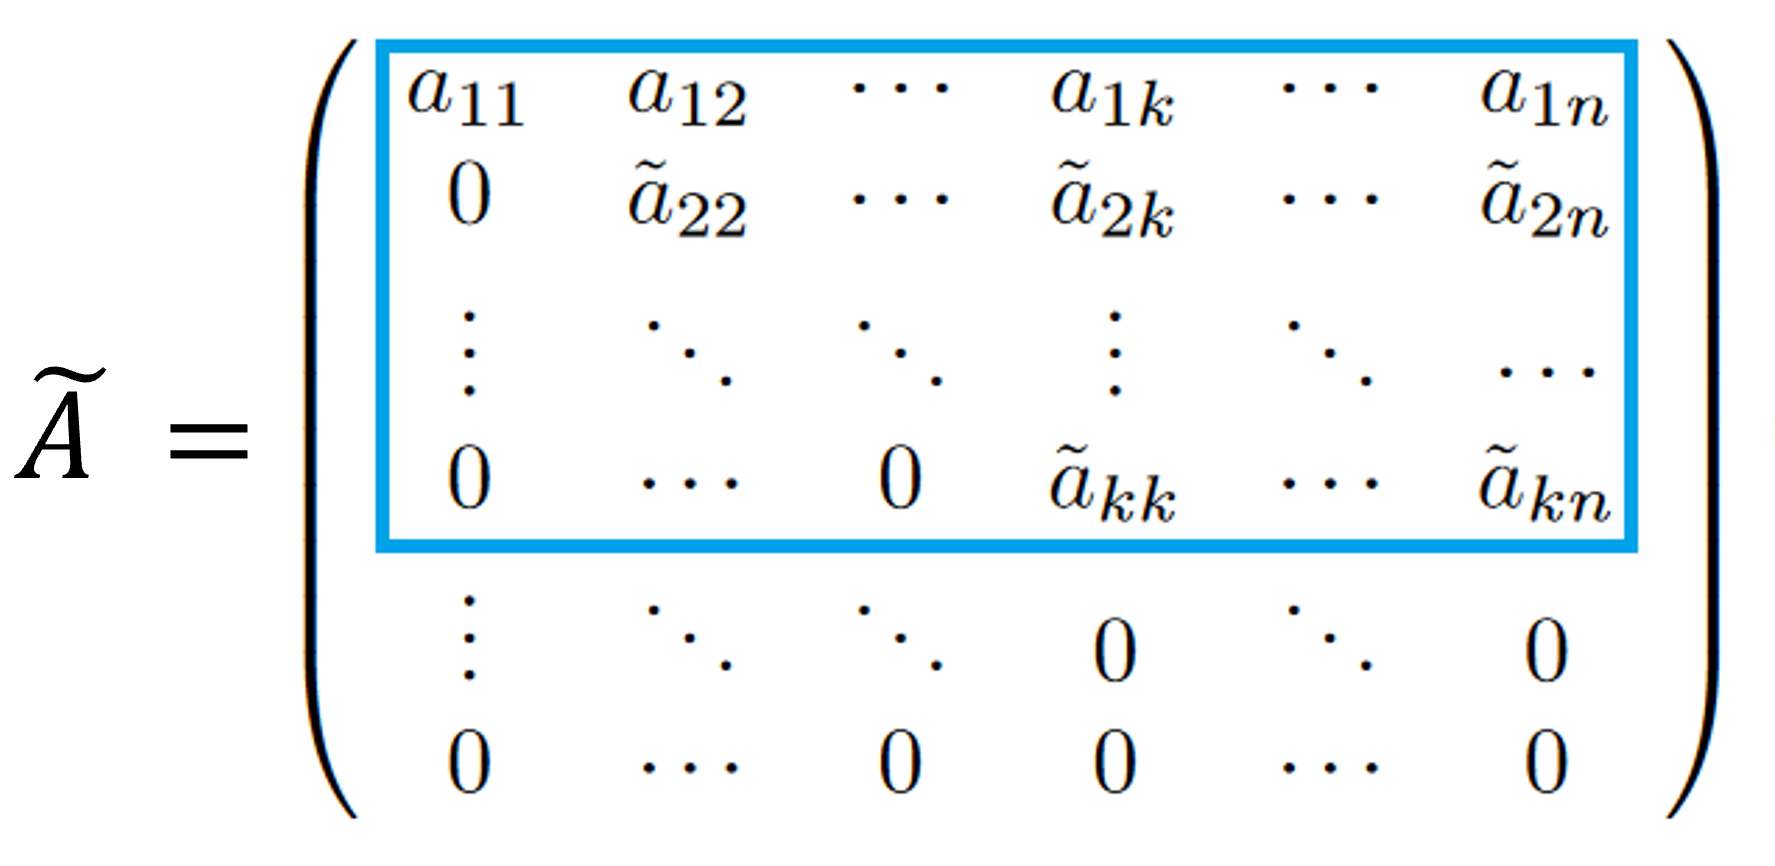
\includegraphics[width=0.4\textwidth]
{../Mathematik_1/Bilder/matrizen_rang_zeilenstufenform.png}
\end{center}

Die Anzahl \(k\) der von Null verschiedenen Zeilen entspricht der Anzahl
der Pivotpositionen und damit dem Rang der Matrix:
\[
\operatorname{rk}(A)=k.
\]

Der zuvor abstrakt als Dimension des Bildes definierte Rang kann damit
mithilfe des Gau�schen Eliminationsverfahrens konkret bestimmt werden.


\subsubsection*{Kern und Defekt bestimmen}

Der Kern einer Matrix wurde definiert durch
\[
\ker(A)
=
\{\vec x\in\mathbb R^n:A\vec x=\vec0\}.
\]

Die Bestimmung des Kerns ist damit nichts anderes als das L�sen des
homogenen linearen Gleichungssystems
\[
A\vec x=\vec0.
\]

Wird \(A\) in Zeilenstufenform gebracht und besitzt die Matrix den Rang
\(k\), so gibt es \(k\) Pivotvariablen. Die �brigen \(n-k\) Variablen sind
freie Variablen.

\begin{center}
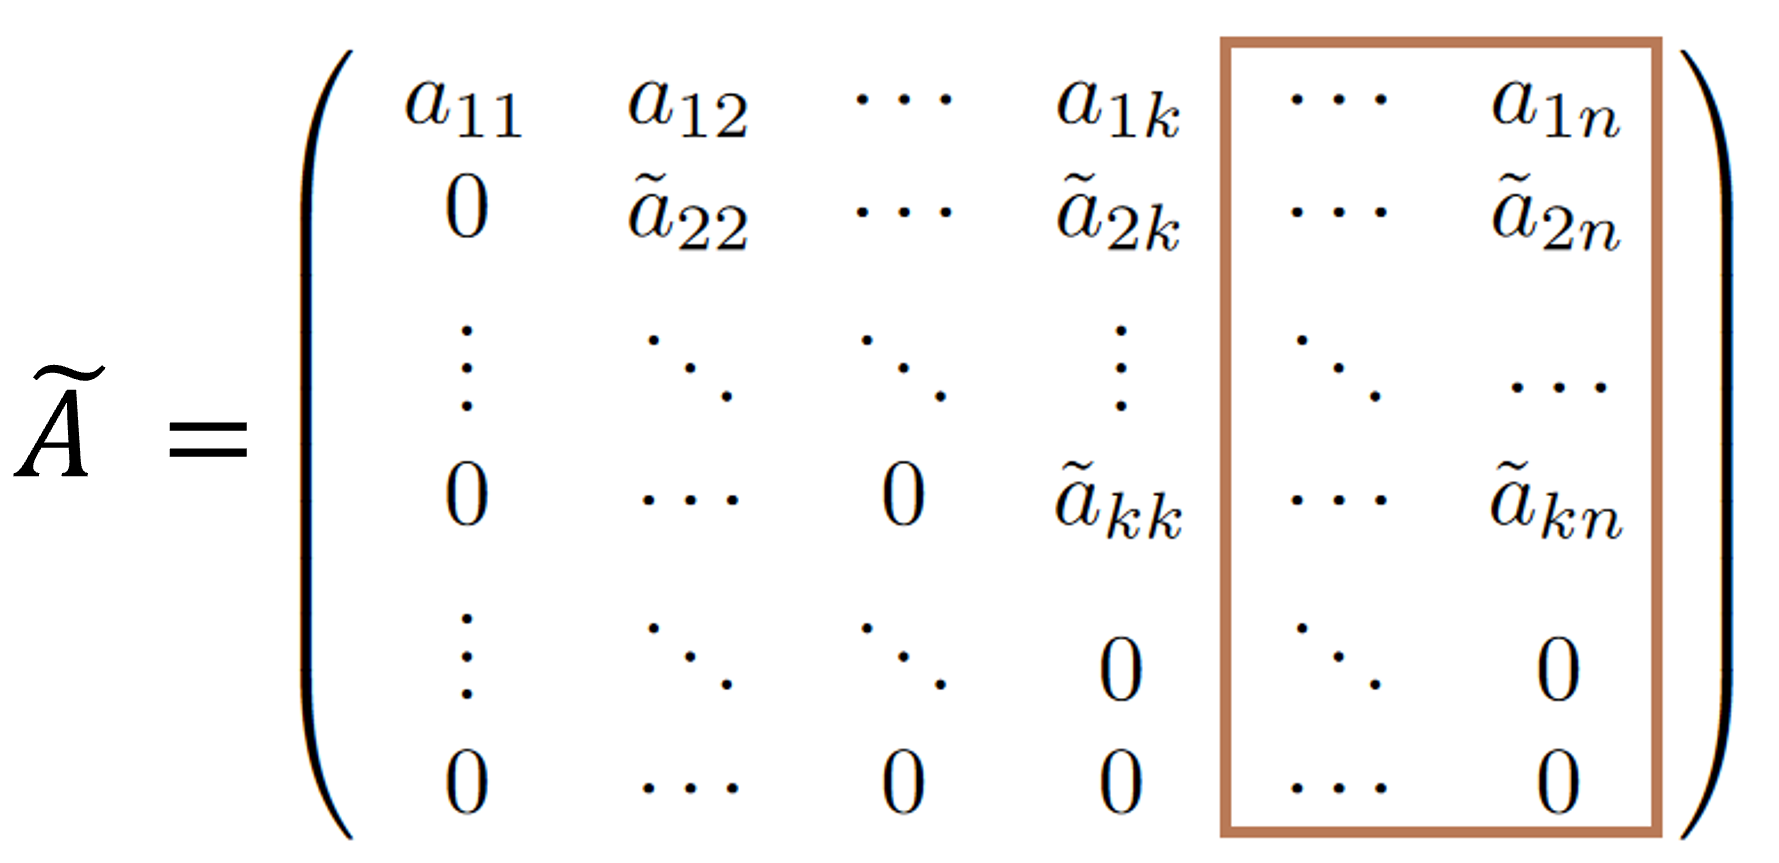
\includegraphics[width=0.4\textwidth]
{../Mathematik_1/Bilder/matrizen_defekt_freie_variablen.png}
\end{center}

Jede freie Variable liefert einen freien Parameter in der allgemeinen
L�sung des homogenen Gleichungssystems. Die Anzahl dieser freien Parameter
entspricht der Dimension des Kerns. Damit gilt
\[
\operatorname{def}(A)
=
\dim\bigl(\ker(A)\bigr)
=
n-k.
\]

Da gleichzeitig
\[
\operatorname{rk}(A)=k
\]
gilt, folgt
\[
\operatorname{rk}(A)+\operatorname{def}(A)=n.
\]

Der Rangsatz erh�lt damit eine unmittelbar sichtbare Bedeutung: Die
\(n\) Variablen zerfallen in \(k\) durch Pivotpositionen bestimmte
Variablen und \(n-k\) freie Variablen. Die Anzahl der freien Parameter
entspricht der Dimension des Kerns.

\subsubsection*{Lineare Unabh�ngigkeit systematisch untersuchen}

Auch die Frage nach der linearen Unabh�ngigkeit mehrerer Vektoren l�sst sich auf ein lineares Gleichungssystem zur�ckf�hren.

Gegeben seien
\[
\vec a_1,\ldots,\vec a_n\in\mathbb R^m.
\]
Nach der Definition sind diese Vektoren genau dann linear unabh�ngig, wenn
aus
\[
x_1\vec a_1+\cdots+x_n\vec a_n=\vec0
\]
notwendig
\[
x_1=\cdots=x_n=0
\]
folgt.

Werden die Vektoren als Spalten einer Matrix
\[
A=
\begin{pmatrix}
\vert&&\vert\\
\vec a_1&\cdots&\vec a_n\\
\vert&&\vert
\end{pmatrix}
\]
angeordnet, so wird die Bedingung zur Matrixgleichung
\[
A\vec x=\vec0.
\]

Damit gilt:
\[
\vec a_1,\ldots,\vec a_n
\text{ sind linear unabh�ngig}
\quad\Longleftrightarrow\quad
\ker(A)=\{\vec0\}.
\]

Die abstrakte Frage nach linearer Unabh�ngigkeit wird dadurch zu einer konkreten Rechenaufgabe: Das zugeh�rige homogene lineare Gleichungssystem wird mit dem Gau�schen Eliminationsverfahren gel�st.

Besitzt es nur die triviale L�sung, sind die Vektoren linear unabh�ngig.  Treten freie Parameter und damit nichttriviale L�sungen auf, sind die Vektoren linear abh�ngig.
\subsubsection*{Das Bild und eine Basis des Bildes bestimmen (+)}

Die Spalten einer Matrix
\[
A=
\begin{pmatrix}
\vert && \vert\\
\vec a_1&\cdots&\vec a_n\\
\vert && \vert
\end{pmatrix}
\]
spannen das Bild der zugeh�rigen linearen Abbildung auf:
\[
\operatorname{im}(A)
=
\operatorname{span}\{\vec a_1,\ldots,\vec a_n\}.
\]

Damit bilden die Spalten von \(A\) zun�chst ein Erzeugendensystem des
Bildes. Dieses Erzeugendensystem muss jedoch nicht linear unabh�ngig sein.
F�r eine Basis des Bildes werden daher gerade so viele linear unabh�ngige
Vektoren ben�tigt, wie der Rang der Matrix angibt.

Das Gau�sche Eliminationsverfahren kann auch verwendet werden, um solche
Basisvektoren systematisch zu bestimmen. Dabei ist zu beachten, dass die
gesuchten Vektoren als \emph{Spalten} in \(A\) stehen, w�hrend das
Gau�verfahren mit \emph{Zeilen} arbeitet.

Deshalb wird zun�chst die transponierte Matrix
\[
A^{\intercal}
\]
gebildet. Die Spaltenvektoren von \(A\) erscheinen darin als Zeilenvektoren.
Anschlie�end wird \(A^{\intercal}\) durch elementare Zeilenumformungen in
Zeilenstufenform �berf�hrt \(A^\intercal \longrightarrow \widetilde{ ( A^\intercal) } \).

\begin{center}
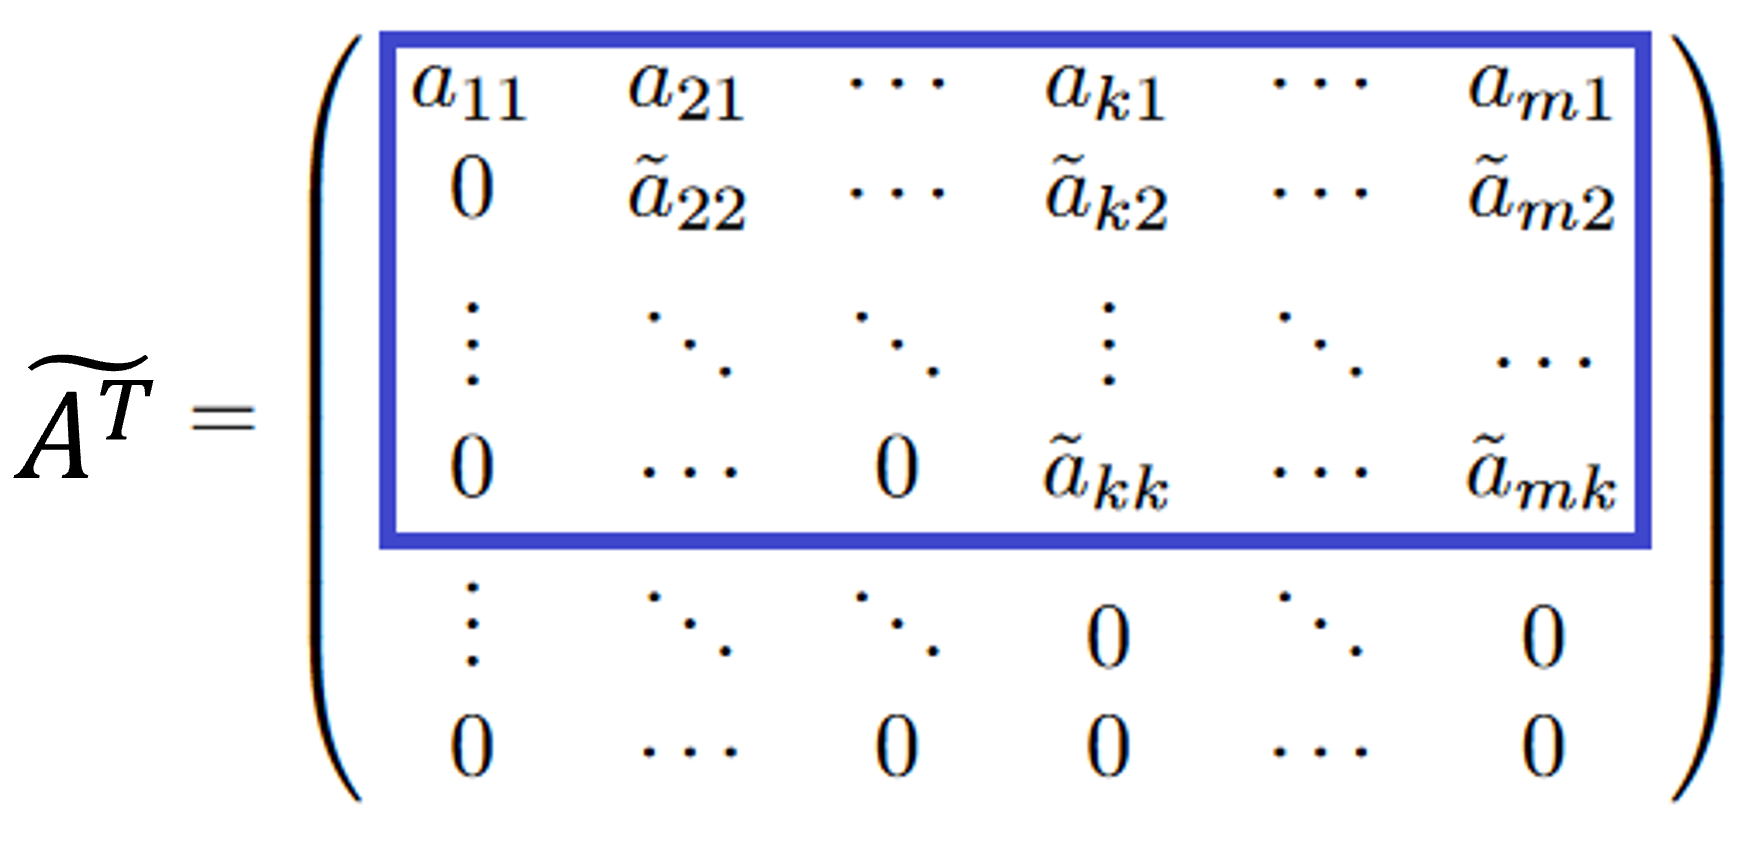
\includegraphics[width=0.4\textwidth]
{../Mathematik_1/Bilder/matrizen_bildbasis_transponierte_zeilenstufenform.png}
\end{center}

Die elementaren Zeilenumformungen ver�ndern den von den Zeilen aufgespannten
Vektorraum nicht. In der Zeilenstufenform bleiben daher genau \(k\)
linear unabh�ngige Nichtnullzeilen �brig, wenn
\[
\operatorname{rk}(A)=k.
\]

Diese \(k\) Zeilen bilden eine Basis des Zeilenraums von
\(A^{\intercal}\). Durch erneutes Transponieren werden daraus
Spaltenvektoren in \(\mathbb R^m\). Diese Vektoren bilden eine Basis des
Bildes von \(A\).

Damit liefert das Gau�sche Eliminationsverfahren nicht nur die Dimension
des Bildes. Durch die Anwendung auf die transponierte Matrix k�nnen auch
konkrete Basisvektoren des Bildes bestimmt werden.


\subsubsection*{Eine gemeinsame Systematik}

Mehrere zuvor getrennt eingef�hrte Begriffe lassen sich damit auf dieselbe Rechenmethode zur�ckf�hren:

\[
A\vec x=\vec b
\quad\longrightarrow\quad
\text{L�sbarkeit und L�sungsmenge},
\]

\[
A\vec x=\vec0
\quad\longrightarrow\quad
\text{Kern und Defekt},
\]

und die Zeilenstufenform von \(A\) liefert Informationen �ber Rang, Pivotspalten und damit �ber lineare Unabh�ngigkeit und eine Basis des Bildes.

Das Gau�sche Eliminationsverfahren ist deshalb nicht nur ein Verfahren zum L�sen linearer Gleichungssysteme. Es ist ein grundlegendes Rechenwerkzeug der linearen Algebra, das die abstrakten Begriffe der vorangegangenen Abschnitte konkret zug�nglich macht.


%----------------------------------------------------------
\subsection*{Ausblick}

�berbestimmte Gleichungssysteme m�ssen nicht l�sbar sein. In vielen Anwendungen entsteht dann die Frage, ob zumindest ein Vektor gefunden werden kann, der die Gleichungen m�glichst gut erf�llt. Dies f�hrt zur \textbf{Methode der kleinsten Fehlerquadrate} (\emph{least squares}), die beispielsweise bei der linearen Regression eine
zentrale Rolle spielt.

Das Gau�sche Eliminationsverfahren ist ein \textbf{direktes L�sungsverfahren}. Bei exakter Arithmetik wird nach endlich vielen Eliminationsschritten eine Form erreicht, aus der sich die L�sungsstruktur bestimmen l�sst. Bei numerischen Rechnungen mit Gleitkommazahlen kommen zus�tzlich Rundungsfehler und Fragen der numerischen Stabilit�t hinzu.

F�r sehr gro�e lineare Gleichungssysteme k�nnen dagegen \textbf{iterative Verfahren} (\emph{iterative methods}) zweckm��ig sein.  Dabei wird ausgehend von einem Startwert eine Folge von N�herungen erzeugt, die unter geeigneten Voraussetzungen gegen die gesuchte L�sung konvergiert.

Ein grundlegendes Beispiel ist das \textbf{Jacobi-Verfahren} (\emph{Jacobi method}). F�r bestimmte Klassen quadratischer Matrizen konvergiert dieses Verfahren zur L�sung des Gleichungssystems. Eine hinreichende Bedingung ist beispielsweise strikte Diagonaldominanz der Matrix. Die Untersuchung solcher Verfahren und ihrer Konvergenzeigenschaften geh�rt zur numerischen Mathematik.

  % Lineare Gleichungssysteme
\newpage % Linerae Gleichungssysteme
\setcounter{satz}{0} \setcounter{def}{0} \setcounter{exa}{0}  
\section{Determinante und Inverse (+)}\label{MA1-determinante-und-inverse}

\begin{table}[H]
  \centering
  \begin{tabularx}{\textwidth}{p{0.9\textwidth} p{0.1\textwidth}}
    \toprule
    \multicolumn{2}{c}{\textbf{�bersicht �ber Lernziele und Voraussetzungen}}\\
    \midrule
    \textbf{Lernziele} &\\[.5\normalbaselineskip]
    \tabitem die Determinante einer quadratischen Matrix berechnen und geometrisch interpretieren &\\
    \tabitem den Zusammenhang zwischen Determinante, Rang und Invertierbarkeit erl�utern &\\
    \tabitem die Bedeutung der inversen Matrix als Darstellung der Umkehrabbildung erkl�ren &\\
    \tabitem die inverse Matrix zur L�sung linearer Gleichungssysteme interpretieren &\\
    \midrule
    \textbf{Voraussetzungen} &\\[.5\normalbaselineskip]
    \tabitem Umkehrfunktion & \abschnittsverweis{MA1-eigenschaften-von-funktionen}\\
    \tabitem Rang und Defekt einer Matrix & \abschnittsverweis{MA1-matrizen}\\
    \tabitem Gau�sches Eliminationsverfahren & \abschnittsverweis{MA1-lineare-gleichungssysteme}\\
    \bottomrule
  \end{tabularx}
\end{table}

\ifintegriereaufgaben
\noindent �bungsaufgaben zum Thema finden sich hier:
\hyperref[MA1-determinante-und-inverse-aufgaben]{Aufgaben}
\vspace{0.3cm}
\hrule
\fi


\subsection{Was ist die Determinante?}

Eine quadratische Matrix
\[
A\in\mathbb R^{n\times n}
\]
beschreibt eine lineare Abbildung
\[
\mathcal A:\mathbb R^n\to\mathbb R^n,
\qquad
\vec x\mapsto A\vec x.
\]
Eine solche Abbildung kann den Raum beispielsweise strecken, stauchen,
scheren oder spiegeln. Dabei ver�ndert sie im Allgemeinen auch Fl�chen
beziehungsweise Volumina.

Die \textbf{Determinante} (\emph{determinant}) ordnet jeder quadratischen
Matrix eine reelle Zahl zu:
\begin{defbox}{Determinante}{ }
\[
\det:\mathbb R^{n\times n}\to\mathbb R,
\qquad
A\mapsto\det(A).
\]
\end{defbox}

Diese zun�chst abstrakt erscheinende Zahl besitzt eine anschauliche
geometrische Bedeutung. Sie beschreibt, wie die zu \(A\) geh�rende lineare
Abbildung orientierte Volumina ver�ndert.

\begin{defbox}{Geometrische Bedeutung der Determinante}{ }
\begin{itemize}
    \item Der Betrag \(|\det(A)|\) gibt an, um welchen Faktor
    \(n\)-dimensionale Volumina durch die lineare Abbildung ver�ndert
    werden. F�r \(n=2\) sind dies Fl�cheninhalte, f�r \(n=3\) Volumina.

    \item Das Vorzeichen der Determinante beschreibt, ob die Orientierung
    erhalten bleibt oder umgekehrt wird.

    \item F�r \(\det(A)=0\) wird das \(n\)-dimensionale Volumen vollst�ndig
    auf null zusammengedr�ckt. Das Bild der linearen Abbildung besitzt dann
    eine kleinere Dimension als der Ausgangsraum.
\end{itemize}

\begin{center}
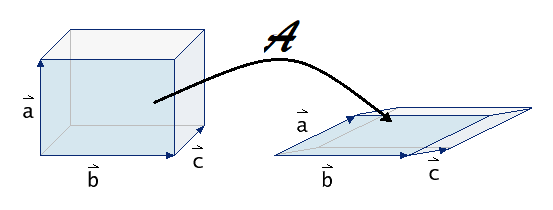
\includegraphics[width=0.6\textwidth]
{../Mathematik_1/Bilder/determinante_volumenverlust_dimension.png}
\end{center}
\end{defbox}

Gerade der letzte Fall wird sp�ter eine besondere Bedeutung erhalten:
Wenn \(\det(A)=0\) gilt, geht durch die lineare Abbildung mindestens eine
Raumrichtung verloren. Die Abbildung kann dann nicht umkehrbar sein.

F�r einfache geometrische Transformationen
\[
\mathcal A:\mathbb R^2\to\mathbb R^2,
\qquad
\vec x\mapsto A\vec x,
\]
l�sst sich die Determinante bereits aus der geometrischen Wirkung der
Abbildung verstehen.

\begin{exabox}{Determinanten f�r einfache geometrische Transformationen}{ }
\begin{eqnarray*}
\left| \begin{array}{cc} 0 & 0 \\ 0 & 0 \end{array}\right|
&=&0\,,
\quad \textnormal{Nullabbildung},\\
\left| \begin{array}{cc} 1 & 0 \\ 0 & 1 \end{array}\right|
&=&1\,,
\quad \textnormal{Identit�tsabbildung},\\
\left| \begin{array}{cc} 2 & 0 \\ 0 & 2 \end{array}\right|
&=&4\,,
\quad \textnormal{Skalierung in zwei Richtungen},\\
\left| \begin{array}{cc} 2 & 0 \\ 0 & 1 \end{array}\right|
&=&2\,,
\quad \textnormal{Skalierung in einer Koordinatenrichtung},\\
\left| \begin{array}{cc}
\frac{1}{\sqrt{2}} &-\frac{1}{\sqrt{2}}\\
\frac{1}{\sqrt{2}} & \frac{1}{\sqrt{2}}
\end{array}\right|
&=&1\,,
\quad \textnormal{Drehung},\\
\left| \begin{array}{cc} 0&1\\1&0\end{array}\right|
&=&-1\,,
\quad \textnormal{Spiegelung},\\
\left| \begin{array}{cc}1&1\\0&1\end{array}\right|
&=&1\,,
\quad \textnormal{Scherung in einer Achsenrichtung}.
\end{eqnarray*}
\end{exabox}

Die Beispiele zeigen bereits zwei unterschiedliche Informationen der
Determinante. Eine Drehung und eine Scherung k�nnen den Fl�cheninhalt
unver�ndert lassen und besitzen daher den Betrag \(1\). Eine Spiegelung
l�sst den Fl�cheninhalt ebenfalls unver�ndert, kehrt jedoch die Orientierung
um und besitzt deshalb eine negative Determinante.


\subsection{Eigenschaften und Berechnung der Determinante}

Werden zwei lineare Abbildungen hintereinander ausgef�hrt, so
multiplizieren sich ihre Volumenskalierungsfaktoren. Entsprechend gilt f�r
quadratische Matrizen \(A\) und \(B\):

\begin{theorembox}{Determinante eines Produkts}{ }
\[
\det(AB)=\det(A)\cdot\det(B).
\]
\end{theorembox}

Hieraus und aus den grundlegenden Eigenschaften der Determinante ergeben
sich Rechenregeln f�r Ver�nderungen einzelner Spalten beziehungsweise
Zeilen.

\begin{exabox}{Rechenregeln}{ }
\begin{enumerate}

\item Wird eine Spalte oder Zeile mit einem Faktor \(\lambda\)
multipliziert, so wird auch die Determinante mit \(\lambda\) multipliziert:
\begin{eqnarray*}
\left| \begin{array}{ccc}
2&-7&\textcolor{blue}{3}\\
0&2&\textcolor{blue}{6}\\
4&1&\textcolor{blue}{9}
\end{array}\right|
=
\textcolor{blue}{3}
\left| \begin{array}{ccc}
2&-7&1\\
0&2&2\\
4&1&3
\end{array}\right|.
\end{eqnarray*}

\item Werden zwei Spalten oder Zeilen vertauscht, so wechselt das
Vorzeichen der Determinante:
\begin{eqnarray*}
\left| \begin{array}{ccc}
2&\textcolor{blue}{-7}&\textcolor{brown}{3}\\
0&\textcolor{blue}{2}&\textcolor{brown}{6}\\
4&\textcolor{blue}{1}&\textcolor{brown}{9}
\end{array}\right|
=
-
\left| \begin{array}{ccc}
2&\textcolor{brown}{3}&\textcolor{blue}{-7}\\
0&\textcolor{brown}{6}&\textcolor{blue}{2}\\
4&\textcolor{brown}{9}&\textcolor{blue}{1}
\end{array}\right|.
\end{eqnarray*}

\item Besitzt eine Matrix zwei identische Spalten oder Zeilen, so
verschwindet ihre Determinante:
\begin{eqnarray*}
\alpha
&=&
\left| \begin{array}{ccc}
\textcolor{blue}{2}&-7&\textcolor{brown}{2}\\
\textcolor{blue}{0}&2&\textcolor{brown}{0}\\
\textcolor{blue}{4}&1&\textcolor{brown}{4}
\end{array}\right| \\
&=&
-
\left| \begin{array}{ccc}
\textcolor{brown}{2}&-7&\textcolor{blue}{2}\\
\textcolor{brown}{0}&2&\textcolor{blue}{0}\\
\textcolor{brown}{4}&1&\textcolor{blue}{4}
\end{array}\right|
=-\alpha,
\end{eqnarray*}
also \(\alpha=0\).

\item Die Determinante ist in jeder einzelnen Spalte beziehungsweise Zeile
linear. Ist beispielsweise eine Spalte die Summe zweier Vektoren, so kann
die Determinante entsprechend zerlegt werden:
\begin{eqnarray*}
\left| \begin{array}{cc}2&2\\3&5\end{array}\right|
&=&
\left| \begin{array}{cc}\textcolor{blue}{2+}0&2\\
\textcolor{blue}{1+}2&5\end{array}\right|\\
&=&
\left| \begin{array}{cc}\textcolor{blue}{2}&2\\
\textcolor{blue}{1}&5\end{array}\right|
\textcolor{blue}{+}
\left| \begin{array}{cc}0&2\\2&5\end{array}\right|.
\end{eqnarray*}

\item Wird zu einer Spalte oder Zeile ein Vielfaches einer anderen Spalte
beziehungsweise Zeile addiert, so ver�ndert sich die Determinante nicht.
Diese Eigenschaft ist insbesondere bei der Berechnung von Determinanten
mithilfe des Gau�schen Eliminationsverfahrens n�tzlich.

\end{enumerate}
\end{exabox}

\noindent\textbf{Bemerkungen:}
\begin{itemize}
    \item Es gilt
    \[
    \det(A)=\det(A^\intercal).
    \]
    Daher gelten die entsprechenden Rechenregeln gleicherma�en f�r
    Spalten und Zeilen.

    \item Die Determinante ist in ihren Spalten beziehungsweise Zeilen
    multilinear und alternierend. Insbesondere verschwindet sie, sobald
    zwei Spalten beziehungsweise zwei Zeilen identisch sind.
\end{itemize}


\subsubsection*{Determinante einer \(2\times2\)-Matrix}

Die Rechenregeln erm�glichen nun die Berechnung konkreter Determinanten.
F�r eine \(2\times2\)-Matrix ergibt sich beispielsweise
\begin{eqnarray*}
\left| \begin{array}{cc}
\textcolor{blue}{1}&\textcolor{brown}{2}\\
\textcolor{brown}{3}&\textcolor{blue}{4}
\end{array}\right|
&=&
\textcolor{blue}{1}\cdot\textcolor{blue}{4}
-
\textcolor{brown}{2}\cdot\textcolor{brown}{3}\\
&=&-2.
\end{eqnarray*}

Allgemein gilt damit:

\begin{defbox}{Determinante einer \(2\times2\)-Matrix}{ }
\[
\left|
\begin{array}{cc}
\textcolor{blue}{a}&\textcolor{brown}{b}\\
\textcolor{brown}{c}&\textcolor{blue}{d}
\end{array}
\right|
=
\textcolor{blue}{a}\cdot\textcolor{blue}{d}
-
\textcolor{brown}{b}\cdot\textcolor{brown}{c}.
\]
\end{defbox}


\subsubsection*{Entwicklung einer \(3\times3\)-Determinante}

Eine \(3\times3\)-Determinante kann auf \(2\times2\)-Determinanten
zur�ckgef�hrt werden. Bei einer Entwicklung nach der ersten Spalte ergibt
sich beispielsweise

\begin{exabox}{Entwicklung nach der ersten Spalte}{ }
\begin{eqnarray*}
\left|
\begin{array}{ccc}
\textcolor{blue}{1}&2&3\\
\textcolor{blue}{4}&5&6\\
\textcolor{blue}{7}&8&9
\end{array}
\right|
&=&
\textcolor{blue}{1}
\left|\begin{array}{cc}5&6\\8&9\end{array}\right|
-
\textcolor{blue}{4}
\left|\begin{array}{cc}2&3\\8&9\end{array}\right|
+
\textcolor{blue}{7}
\left|\begin{array}{cc}2&3\\5&6\end{array}\right|\\
&=&
(5\cdot9-6\cdot8)
-4(2\cdot9-3\cdot8)
+7(2\cdot6-3\cdot5)\\
&=&-3+24-21=0.
\end{eqnarray*}
\end{exabox}

Entsprechend kann eine Determinante nach jeder Zeile oder Spalte entwickelt
werden. Das Vorzeichen des jeweiligen Terms h�ngt von seiner Position ab
und folgt dem Schachbrettmuster:

\begin{theorembox}{Vorzeichen im Schachbrettmuster}{ }
\[
\left|
\begin{array}{ccc}
+&-&+\\
-&+&-\\
+&-&+
\end{array}
\right|.
\]
\end{theorembox}

F�r \(3\times3\)-Determinanten ergibt sich au�erdem die leicht zu merkende
\textbf{Regel von Sarrus}:

\begin{eqnarray*}
\left|
\begin{array}{ccc}
1&2&3\\
4&5&6\\
7&8&9
\end{array}
\right|
\textcolor{lightgray}{
\begin{array}{cc}
1&2\\4&5\\7&8
\end{array}}
=
\textcolor{red}{1\cdot5\cdot9+2\cdot6\cdot7+3\cdot4\cdot8}
\textcolor{blue}{-7\cdot5\cdot3-8\cdot6\cdot1-9\cdot4\cdot2}.
\end{eqnarray*}

Die Regel von Sarrus gilt ausschlie�lich f�r \(3\times3\)-Matrizen. Sie
l�sst sich nicht auf Determinanten der Gr��e \(4\times4\) oder h�her
�bertragen.

Bei einer direkten Entwicklung einer \(n\times n\)-Determinante entstehen
\(n!\) Produkte mit jeweils \(n\) Faktoren. Der Rechenaufwand w�chst daher
sehr schnell. F�r gr��ere Matrizen ist eine vollst�ndige Entwicklung
deshalb kein zweckm��iges Berechnungsverfahren.

Eine Alternative ergibt sich aus dem bereits bekannten Gau�schen
Eliminationsverfahren. Wird eine Matrix unter Beachtung der oben
angegebenen Rechenregeln auf Dreiecksgestalt gebracht, so l�sst sich die
Determinante anschlie�end unmittelbar aus den Diagonaleintr�gen bestimmen.
F�r eine Dreiecksmatrix gilt
\[
\det(A)=a_{11}a_{22}\cdots a_{nn}.
\]


\subsubsection*{Das Spatprodukt (+)}

Mit der Determinante l�sst sich eine weitere geometrische Verkn�pfung von
Vektoren beschreiben. Das \textbf{Spatprodukt} (\emph{triple product}) ist
eine Besonderheit des \(\mathbb R^3\) und bildet drei Vektoren auf eine
reelle Zahl ab.

Sind \(\vec x_1,\vec x_2,\vec x_3\in\mathbb R^3\), so werden diese als
Spalten einer Matrix zusammengefasst:

\begin{defbox}{Spatprodukt}{ }
\[
\mathbb R^3\times\mathbb R^3\times\mathbb R^3\to\mathbb R,
\qquad
(\vec x_1,\vec x_2,\vec x_3)
\mapsto
\det(\vec x_1,\vec x_2,\vec x_3).
\]
\end{defbox}

Beispielsweise gilt

\begin{exabox}{Spatprodukt}{ }
\[
\left|
\begin{array}{ccc}
1&3&4\\
2&0&-2\\
3&2&1
\end{array}
\right|
=-4.
\]
\end{exabox}

Der Betrag des Spatprodukts liefert das Volumen des von den drei Vektoren
aufgespannten Parallelepipeds. Das Vorzeichen beschreibt zus�tzlich die
Orientierung der drei Vektoren.


\subsection{Inverse Matrix}

F�r ein quadratisches lineares Gleichungssystem
\[
A\vec x=\vec b,
\qquad
A\in\mathbb R^{n\times n},
\]
wurde im vorangegangenen Abschnitt gezeigt, dass die L�sbarkeit und
Eindeutigkeit der L�sung eng mit Rang und Kern der Koeffizientenmatrix
zusammenh�ngen.

F�r quadratische Matrizen liefert die Determinante nun ein besonders
kompaktes Kriterium. Ist
\[
\det(A)=0,
\]
so wird mindestens eine Raumrichtung durch die zugeh�rige lineare Abbildung
verloren. Das Bild besitzt eine Dimension kleiner als \(n\), also
\[
\operatorname{rk}(A)<n.
\]
Die Abbildung kann deshalb nicht bijektiv und damit auch nicht umkehrbar
sein.

Ist dagegen
\[
\det(A)\neq0,
\]
so geht keine Raumrichtung verloren. Die Matrix besitzt vollen Rang,
\[
\operatorname{rk}(A)=n,
\]
und die zugeh�rige lineare Abbildung
\[
\mathcal A:\mathbb R^n\to\mathbb R^n,
\qquad
\vec x\mapsto A\vec x,
\]
ist bijektiv.

Damit sind f�r eine quadratische Matrix mehrere der bisher eingef�hrten
Begriffe unmittelbar miteinander verbunden:

\begin{theorembox}{Determinante und Invertierbarkeit}{ }
F�r \(A\in\mathbb R^{n\times n}\) sind die folgenden Aussagen �quivalent:
\[
\begin{aligned}
\det(A)&\neq0\\
&\Longleftrightarrow\operatorname{rk}(A)=n\\
&\Longleftrightarrow\operatorname{def}(A)=0\\
&\Longleftrightarrow\ker(A)=\{\vec0\}\\
&\Longleftrightarrow\mathcal A:\mathbb R^n\to\mathbb R^n
   \text{ ist bijektiv}\\
&\Longleftrightarrow A\text{ ist invertierbar}.
\end{aligned}
\]
\end{theorembox}

Damit erh�lt die Determinante eine zweite Bedeutung neben ihrer
geometrischen Interpretation: Sie entscheidet bei einer quadratischen
Matrix mit einer einzigen Zahl dar�ber, ob die zugeh�rige lineare Abbildung
umkehrbar ist.


\subsubsection*{Die Inverse als Umkehrabbildung}

Ist \(\det(A)\neq0\), so ist die lineare Abbildung
\[
\mathcal A:\mathbb R^n\to\mathbb R^n,
\qquad
\vec x\mapsto A\vec x,
\]
bijektiv. Zu jedem \(\vec b\in\mathbb R^n\) existiert daher genau ein
\(\vec x\in\mathbb R^n\) mit
\[
A\vec x=\vec b.
\]

Die Umkehrabbildung
\[
\mathcal A^{-1}:\mathbb R^n\to\mathbb R^n
\]
ordnet jedem \(\vec b\) wieder den eindeutig bestimmten Ausgangsvektor
\(\vec x\) zu. Auch diese Umkehrabbildung ist linear und kann deshalb
wieder durch eine Matrix dargestellt werden. Diese Matrix ist die
\textbf{inverse Matrix} (\emph{inverse matrix}) \(A^{-1}\).

\begin{defbox}{Inverse Matrix}{ }
Eine quadratische Matrix \(A\in\mathbb R^{n\times n}\) hei�t
\textbf{invertierbar} (\emph{invertible}), wenn eine Matrix
\(A^{-1}\in\mathbb R^{n\times n}\) existiert mit
\[
A^{-1}A=AA^{-1}=I_n.
\]
Die Matrix \(A^{-1}\) ist die Matrixdarstellung der Umkehrabbildung
\(\mathcal A^{-1}\).
\end{defbox}

Die Schreibweise \(A^{-1}\) erinnert bewusst an den Kehrwert einer Zahl.
F�r eine Zahl \(a\neq0\) gilt
\[
a^{-1}a=aa^{-1}=1.
\]
Bei einer invertierbaren Matrix �bernimmt die Einheitsmatrix \(I_n\) die
Rolle der Zahl \(1\):
\[
A^{-1}A=AA^{-1}=I_n.
\]

Der entscheidende Unterschied zu einer einzelnen L�sung eines linearen
Gleichungssystems besteht darin, dass \(A^{-1}\) nur von der Matrix \(A\)
und nicht von der rechten Seite \(\vec b\) abh�ngt.


\subsubsection*{Die Inverse als Werkzeug zum L�sen linearer Gleichungssysteme}

Ist \(A\) invertierbar, so kann das lineare Gleichungssystem
\[
A\vec x=\vec b
\]
von links mit \(A^{-1}\) multipliziert werden:
\[
A^{-1}A\vec x=A^{-1}\vec b.
\]
Mit \(A^{-1}A=I_n\) folgt
\[
\vec x=A^{-1}\vec b.
\]

\begin{theorembox}{L�sung mit der inversen Matrix}{ }
Ist \(A\in\mathbb R^{n\times n}\) invertierbar, so besitzt
\[
A\vec x=\vec b
\]
f�r jede rechte Seite \(\vec b\in\mathbb R^n\) genau eine L�sung. Sie ist
gegeben durch
\[
\vec x=A^{-1}\vec b.
\]
\end{theorembox}

Damit beschreibt \(A^{-1}\) nicht nur die Umkehrung einer einzelnen
Zuordnung. Die inverse Matrix enth�lt die Umkehrabbildung f�r
\emph{alle} m�glichen rechten Seiten gleichzeitig.

Ist \(A^{-1}\) einmal bekannt, so kann f�r jede neue rechte Seite
\(\vec b\) unmittelbar der zugeh�rige L�sungsvektor
\[
\vec x=A^{-1}\vec b
\]
bestimmt werden. Genau darin liegt die besondere Bedeutung der inversen
Matrix im Zusammenhang mit linearen Gleichungssystemen.

\noindent\textbf{Bemerkung:}
Die inverse Matrix kann beispielsweise mit dem Gau�schen
Eliminationsverfahren bestimmt werden. Dazu wird die erweiterte Matrix
\[
(A\,|\,I_n)
\]
so lange durch elementare Zeilenumformungen ver�ndert, bis auf der linken
Seite die Einheitsmatrix steht:
\[
(A\,|\,I_n)
\longrightarrow
(I_n\,|\,A^{-1}).
\]
Die konkrete Berechnung der inversen Matrix steht hier jedoch nicht im
Vordergrund. Entscheidend ist ihre Bedeutung als Matrixdarstellung der
Umkehrabbildung.


\subsection{Cramersche Regel (+)}

Die Determinante erm�glicht auch eine direkte Darstellung der einzelnen
Komponenten der L�sung eines quadratischen linearen Gleichungssystems
\[
A\vec x=\vec b,
\qquad
\det(A)\neq0.
\]

Wird in \(A\) die \(i\)-te Spalte durch die rechte Seite \(\vec b\)
ersetzt und die so entstehende Matrix mit \(A_i\) bezeichnet, so gilt die
\textbf{Cramersche Regel} (\emph{Cramer's rule})
\[
x_i=\frac{\det(A_i)}{\det(A)},
\qquad i=1,\ldots,n.
\]

Die Cramersche Regel macht den Zusammenhang zwischen Determinante und
eindeutiger L�sbarkeit besonders deutlich. F�r gr��ere Gleichungssysteme
ist sie jedoch kein zweckm��iges numerisches L�sungsverfahren; hierf�r
werden beispielsweise Verfahren auf Grundlage der Gau�-Elimination
verwendet.



% \section{Determinante und Inverse (+)}\label{MA1-determinante-und-inverse}
% 
% \begin{table}[H]
%   \centering
%   \begin{tabularx}{\textwidth}{p{0.9\textwidth} p{0.1\textwidth}}
%     \toprule
% 	  \multicolumn{2}{c}{\textbf{�bersicht �ber Lernziele und Voraussetzungen}}\\
%     \midrule
% \textbf{Lernziele} &\\[.5\normalbaselineskip]
% \tabitem die Determinante einer quadratischen Matrix berechnen und
% geometrisch interpretieren &\\
% \tabitem den Zusammenhang zwischen Determinante, Rang und Invertierbarkeit
% einer quadratischen Matrix erkl�ren &\\
% \tabitem die Invertierbarkeit einer quadratischen Matrix untersuchen &\\
% \tabitem die inverse Matrix mithilfe des Gau�schen Eliminationsverfahrens
% bestimmen (+) &\\
% \tabitem die Cramersche Regel erkl�ren und auf lineare Gleichungssysteme
% anwenden (+) &\\
%     \midrule
% 	  \textbf{Sie sollten bereits \ldots} &\\[.5\normalbaselineskip]
%     \tabitem Umkehrfunktion & \abschnittsverweis{MA1-eigenschaften-von-funktionen}\\
%     \tabitem Rang und Defekt einer Matrix & \abschnittsverweis{MA1-matrizen}\\
%     \tabitem Gau�sches Eliminationsverfahren & \abschnittsverweis{MA1-lineare-gleichungssysteme}\\
%     \bottomrule
%   \end{tabularx}
% \end{table}
% 
% \ifintegriereaufgaben \noindent �bungsaufgaben zum Thema finden Sie hier: \hyperref[MA1-determinante-und-inverse-aufgaben]{Aufgaben}
% \vspace{0.3cm}
% \hrule
%  \fi
% 
% \subsection{Was ist die Determinante?}
% 
% Die Determinante [determinant] ordnet jeder quadratischen Matrix $A\in\mathbb R^{n\times n}$ eine Zahl zu
% \begin{defbox}{Determinante}{ }
% 	$\mathrm{det}: \; \mathbb R^{n\times n} \to \mathbb R, \; \left( \begin{array}{cc} 1  & 2 \\ 3 &   4\end{array}\right) \mapsto \left| \begin{array}{cc} 1  & 2 \\ 3 &   4\end{array}\right|\,. $
% \end{defbox}
% Die Determinante sagt etwas �ber die "\,Gr��e"\, der Matrix $A$ aus und sie liefert ein notwendiges und hinreichendes Kriterium f�r die Existenz der inversen Matrix $A^{-1}$. Diese Eigenschaft vereinfacht die Frage nach der L�sbarkeit eines linearen Gleichungssystems mit quadratischer Koeffizientenmatrix $A$.\marginpar{\small Aufgaben}
% 
% %Wenn die Matrix �ber ihre Elemente gegeben ist, schreibt man die Determinante auch mit Strichen um die Elemente der Matrix: 
% 
% %Also Vorsicht: Runde Klammern oder in den USA eckige Klammern bezeichnen eine Matrix, Striche links und rechts dagegen eine daraus berechnete Zahl, n�mlich die Determinante der Matrix. %In MATLAB hei�t die Funktion zum Berechnen von Determinenten schlicht \verb-det-. In Wolfram Alpha kann man ebenfalls \verb-det- schreiben. 
% 
% Auch wenn die Schreibweise mit den Strichen an einen Betrag erinnert, ist die Determinante etwas Anderes. Sie gibt Aufschluss �ber zwei geometrische Eigenschaften, die eine lineare Abbildung auf eine Figur hat:
% \begin{defbox}{Determinante}{ }
% 	\begin{itemize}
% 		\item  Der Betrag der Determinante, also ihr Wert ohne Vorzeichen, sagt aus, um welchen Faktor die lineare Abbildung \(\mathcal A\) die Fl�che ($n=2$), bzw. das Volumen ($n=3$) ver�ndert.  
%     \item Das Vorzeichen der Determinante sagt aus, ob die lineare Abbildung \(\mathcal A\) die Orientierung ver�ndert. F�r $n=2$ entspricht die Ver�nderung der Orientierung eine Spiegelung, f�r $n=3$ ist die "rechte-Hand-Regel" gemeint.
%      \end{itemize}
% 	\begin{center}
% 	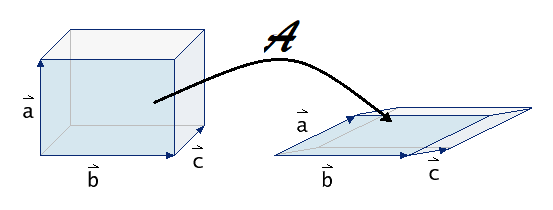
\includegraphics[width=0.6\textwidth]{../Mathematik_1/Bilder/determinante_volumenverlust_dimension.png}
% \end{center}
% \end{defbox}
% 
% F�r einfache geometrische Transformation \(\mathcal A: \mathbb R^2 \to \mathbb R^2, \vec x \to A\vec x\) l��t sich \(\mathrm{det}(A)\) ohne Rechnung angeben:
% \begin{exabox}{Determinanten f�r einfache geometrische Transformationen}{ }
%       \begin{eqnarray*}
% 	\left| \begin{array}{cc} 0 & 0 \\ 0 & 0 \end{array}\right| &=& 0\,, \quad \textnormal{Nullmatrix}\,,\\
% 	\left| \begin{array}{cc} 1 & 0 \\ 0 & 1 \end{array}\right| &=& 1\,, \quad \textnormal{Identische Abbildung}\,,\\
% 	\left| \begin{array}{cc} 2 & 0 \\ 0 & 2 \end{array}\right| &=& 4\,,\quad  \textnormal{Skalierung in zwei Richtungen}\,,\\
% 	\left| \begin{array}{cc} 2 & 0 \\ 0 & 1 \end{array}\right| &=& 2\,,\quad \textnormal{Skalierung in eine Richtung}\,,\\
% 	\left| \begin{array}{cc} \frac{1}{\sqrt{2}} &  -\frac{1}{\sqrt{2}} \\ \frac{1}{\sqrt{2}} &  \frac{1}{\sqrt{2}} \end{array}\right| &=& 1\,,\quad \textnormal{Drehung}\,,\\
% 	\left| \begin{array}{cc} 0 &  1 \\ 1 &  0 \end{array}\right| &=& -1\,,\quad \textnormal{Spigelung, i.e. Vertauschung zweier Spalten}\,,\\
% 	\left| \begin{array}{cc} 1 &  1 \\ 0 &  1 \end{array}\right| &=& 1\,,\quad \textnormal{Scherung in eine Achsenrichtung}\,.
%       \end{eqnarray*}
% \end{exabox}
% 
% Die Determinante zweier Matrizen $A$ und $B$, die man hintereinander anwendet ist  
% \begin{theorembox}{Determinante vom Produkt}{ }
%   $\det(AB)= \det(A)\cdot \det(B)\,.$
% \end{theorembox}
% 
% Hieraus folgen Rechenregeln, die f�r die Determinante bei Spalten- oder Zeilenumformungen gelten m�ssen: 
% \begin{exabox}{Rechenregeln}{ }
%   \begin{enumerate}
%     \item Multiplikation einer Spalte (Zeile) einer Matrix mit einer Zahl:
%       \begin{eqnarray*}
%       \left| \begin{array}{ccc} 2 & -7 & \textcolor{blue}{3} \\ 0 & 2 & \textcolor{blue}{6}  \\ 4 & 1 & \textcolor{blue}{9} \end{array}\right| = \left| \begin{array}{ccc} 2 & -7 & \textcolor{blue}{ 1} \\ 0 & 2 & \textcolor{blue}{2}  \\ 4 & 1 & \textcolor{blue}{3} \end{array}\right| \cdot \left| \begin{array}{ccc} 1 & 0 & 0 \\ 0 & 1 & 0  \\ 0 & 0 & \textcolor{blue}{3} \end{array}\right|  = \textcolor{blue}{3}\, \left| \begin{array}{ccc} 2 & -7 & 1 \\ 0 & 2 & 2  \\ 4 & 1 & 3 \end{array}\right| \,.
%       \end{eqnarray*}
%     \item Vertauschen zweier Spalten (Zeilen) einer Matrix:
%       \begin{eqnarray*}
% 	      \left| \begin{array}{ccc} 2 & \textcolor{blue}{-7} & \textcolor{brown}{3} \\ 0 & \textcolor{blue}{2} & \textcolor{brown}{6}  \\ 4 & \textcolor{blue}{1} & \textcolor{brown}{9} \end{array}\right| = \left| \begin{array}{ccc} 2 & \textcolor{brown}{3} & \textcolor{blue}{-7}  \\ 0 & \textcolor{brown}{6} & \textcolor{blue}{2}  \\ 4 & \textcolor{brown}{9} & \textcolor{blue}{1}  \end{array}\right| \cdot \left| \begin{array}{ccc} 1 & 0 & 0  \\ 0 & 0 & \textcolor{brown}{1}  \\ 0 & \textcolor{blue}{1} & 0  \end{array}\right| = -\left| \begin{array}{ccc} 2 & \textcolor{brown}{3} & \textcolor{blue}{-7}  \\ 0 & \textcolor{brown}{6} & \textcolor{blue}{2}  \\ 4 & \textcolor{brown}{9} & \textcolor{blue}{1}  \end{array}\right| \,.
%       \end{eqnarray*}
% \item Zwei identische Spalten (Zeilen):
%       \begin{eqnarray*}
% 	      \alpha =\left| \begin{array}{ccc} \textcolor{blue}{2} & -7 & \textcolor{brown}{2} \\ \textcolor{blue}{0} & 2 & \textcolor{brown}{0} \\ \textcolor{blue}{4} & 1 & \textcolor{brown}{4} \end{array}\right| \stackrel{2.}{=} - \left| \begin{array}{ccc} \textcolor{brown}{2} & -7 & \textcolor{blue}{2} \\ \textcolor{brown}{0} & 2 & \textcolor{blue}{0} \\ \textcolor{brown}{4} & 1 & \textcolor{blue}{4} \end{array}\right| = - \alpha  \; \Leftrightarrow \; \alpha = 0 \,.
%       \end{eqnarray*}
% \item Eine Spalte (Zeile) einer Matrix als Summer zweier Vektoren:
%       \begin{eqnarray*}
% 	      \left| \begin{array}{cc} 2 & 2 \\ 3 & 5  \end{array}\right| = 
% 	      \left| \begin{array}{cc} \textcolor{blue}{2+}0 & 2 \\ \textcolor{blue}{1+}2 & 5  \end{array}\right| =
% 	      \left| \begin{array}{cc} \textcolor{blue}{2} & 2 \\ \textcolor{blue}{1} & 5  \end{array}\right|  \textcolor{blue}{+}
% 	      \left| \begin{array}{cc} 0 & 2 \\ 2 & 5  \end{array}\right| \,.
%       \end{eqnarray*}
% %\item Addition eines Vielfachen einer Spalte (Zeile) auf eine andere Spalte (Zeile) der Matrix:
% %      \begin{eqnarray*}
% %	      \mathrm{det}\left( \begin{array}{ccc} 2 & -7 & 3 - 2\cdot 7 \\ 0 & 2 & 6+2\cdot2  \\ 4 & 1 & 9+2\cdot 1 \end{array}\right) &=& 
% %	      \mathrm{det}\left( \begin{array}{ccc} 2 & -7 & 3 \\ 0 & 2 & 6  \\ 4 & 1 & 9 \end{array}\right) + \underbrace{2 \mathrm{det}\left( \begin{array}{ccc} 2 & -7 & -7 \\ 0 & 2 & 2  \\ 4 & 1 & 1 \end{array}\right)}_{\displaystyle{= 0}} = 
% %	      \mathrm{det}\left( \begin{array}{ccc} 2 & -7 & 3 \\ 0 & 2 & 6  \\ 4 & 1 & 9 \end{array}\right) \,.
% %      \end{eqnarray*}
% \end{enumerate}
% \end{exabox}
% \noindent\textbf{Bemerkungen:}
% \begin{itemize}
% 	\item Es gilt \(\mathrm{det}(A) = \mathrm{det}(A^\intercal)\) und deshalb gelten die Regeln genauso f�r die entsprechenden Zeilenumformungen.
% 	\item Besitzt eine Abbildung genau diese Eigenschaften dann nennt man sie "\,antisymmetrischen Multilinearform". Die Determinante ist also eine antisymmetrische Multilinearform.
% \end{itemize}
% 
% Mit den Rechenregeln kann man nun die Determinante jeder Matrix berechnen. Wir beginnen mit der Determinante einer $2\times2$-Matrix:
%   \begin{eqnarray*}
% 	  \left| \begin{array}{cc} \textcolor{blue}{1} & \textcolor{brown}{2} \\ \textcolor{brown}{3} & \textcolor{blue}{4}  \end{array}\right| &\stackrel{4.}{=}& \left| \begin{array}{cc} 1 & 2+0 \\0 & 0+4  \end{array}\right| +  \left| \begin{array}{cc} 0 & 2+0 \\3 & 0+4  \end{array}\right| \\[1ex] 
% 	  &\stackrel{1.}{=}& 2\cdot \underbrace{\left| \begin{array}{cc} 1 & 1 \\0 & 0  \end{array}\right|}_{=0 \; (3.)}
%     +  4\cdot \underbrace{\left| \begin{array}{cc} 1 & 0 \\0 & 1  \end{array}\right|}_{=1}  
%     +  2\cdot 3 \underbrace{\left| \begin{array}{cc} 0 & 1 \\1 & 0  \end{array}\right|}_{=-1 \;(1.)} 
%     +  3\cdot 4 \underbrace{\left| \begin{array}{cc} 0 & 0 \\1 & 1  \end{array}\right|}_{=0 \; (3.)}\\[1ex] 
%     &=& \textcolor{blue}{1}\cdot \textcolor{blue}{4} - \textcolor{brown}{2}\cdot \textcolor{brown}{3} = -2 \,.
%   \end{eqnarray*}
% Diese Umformungen sind immer m�glich und deshalb gilt allgemein f�r eine $2\times 2$-Determinante:
% \begin{defbox}{Determinante einer $2\times2$ Matrix}{ }
%   $
%   \left| \begin{array}{cc} \textcolor{blue}{a} & \textcolor{brown}{b} \\ \textcolor{brown}{c} & \textcolor{blue}{d}  \end{array}\right|  = \textcolor{blue}{a}\cdot \textcolor{blue}{d} - \textcolor{brown}{b} \cdot \textcolor{brown}{c}\,.
%     $
% \end{defbox}
% 
% Um die Determinante einer $3\times3$-Matrix zu berechnen, zerlegen wir sie in drei $2\times 2$-"\,Unterdeterminanten":
% \begin{exabox}{Entwicklung nach der ersten Spalte}{ }
%   \begin{eqnarray*}
%     \left| \begin{array}{ccc} \textcolor{blue}{1} & 2 & 3 \\\textcolor{blue}{4} & 5 & 6 \\ \textcolor{blue}{7} & 8 & 9  \end{array}\right| 
%       &=& 
%       \left| \begin{array}{ccc} \textcolor{blue}{1} & 2 & 3 \\0 & 5 & 6 \\0 & 8 & 9  \end{array}\right| 
%       + \left| \begin{array}{ccc} 0 & 2 & 3 \\\textcolor{blue}{4} & 5 & 6 \\0 & 8 & 9  \end{array}\right| 
%       + \left| \begin{array}{ccc} 0 & 3 & 3 \\0 & 5 & 6 \\\textcolor{blue}{7} & 8 & 9  \end{array}\right| \\
%       &=& 
%       \textcolor{blue}{1} \cdot \underbrace{\left| \begin{array}{ccc} \textcolor{brown}{1} & 0 & 0 \\0 & 5 & 6 \\0 & 8 & 9  \end{array}\right|}_{\displaystyle{= \textcolor{brown}{1} \cdot \left| \begin{array}{cc} 5 & 6 \\8 & 9  \end{array}\right|} } 
%       +\; \textcolor{blue}{4} \cdot \underbrace{\left| \begin{array}{ccc} 0 & 2 & 3 \\\textcolor{brown}{1} & 0 & 0 \\0 & 8 & 9  \end{array}\right|}_{\displaystyle{ =\textcolor{brown}{- 1}\cdot \left| \begin{array}{cc} 2 & 3 \\8 & 9  \end{array}\right|} }
%       +\; \textcolor{blue}{7} \cdot \underbrace{ \left| \begin{array}{ccc} 0 & 3 & 3 \\0 & 5 & 6 \\\textcolor{brown}{1} & 0 & 0  \end{array}\right| }_{\displaystyle{= \textcolor{brown}{1}\cdot \left| \begin{array}{cc} 3 & 3 \\5 & 6  \end{array}\right|} }\\
%       &=& \textcolor{brown}{1}\cdot \textcolor{blue}{1}\cdot \left| \begin{array}{cc} 5 & 6 \\8 & 9  \end{array}\right| \textcolor{brown}{- 1 }\cdot \textcolor{blue}{4}\cdot \left| \begin{array}{cc} 2 & 3 \\8 & 9  \end{array}\right|+ \textcolor{brown}{1} \cdot\textcolor{blue}{7} \cdot \left| \begin{array}{cc} 3 & 3 \\5 & 6 \end{array}\right| \\
%       &=& (5\cdot 9 - 6\cdot 8)  - 4  \cdot (2\cdot 9 - 8\cdot 3) + 7 \cdot ( 3\cdot 6 - 5\cdot 3) \\ &=& (45-48)-4\cdot (18-24)+7\cdot (18-15) = -3+24 -21 = 0   \,.
%   \end{eqnarray*}
% \end{exabox}
% 
% Diese Vorgehensweise hei�t "\,Entwicklung nach der ersten Spalte". Entsprechend kann man nach jeder anderen Spalten entwickeln, man muss beim Entwickeln nach anderen Spalten unter Umst�nden Zeilen vertauschen und das f�hrt zu Vorzeichenwechseln. Merken Sie sich die Vorzeichen einfach im Schachbrettmuster:
% \begin{theorembox}{Vorzeichen im Schachbrettmuster}{ }
%   $
%     \left| \begin{array}{ccc} + & - & + \\- & + & - \\+ & - & +  \end{array}\right|\,.
%     $
% \end{theorembox}
% 
% %  Analysiert man diese Berechnung, dann stellt man fest, dass Spalten und Zeilen gleichberechtigt sind, dass also 
% %  \begin{itemize}
% %    \item f�r die Reihen die entsprechenden Rechengesetze gelten wie f�r die Zeilen und 
% %    \item die Determinante beim Transponieren gleich bleibt: $$\det(A^\intercal)= \det(A)$$ 
% %  \end{itemize}
% 
%   Mit entsprechenden Umformungen kann man Determinanten beliebiger Gr��e berechnen. F�r eine $3\times 3$-Determinante findet man die leicht zu merkende Regel von Sarrus.
%   \begin{eqnarray*}
%     \left| \begin{array}{ccc} 1 & 2 & 3 \\4 & 5 & 6 \\7 & 8 & 9  \end{array}\right| \textcolor{lightgray}{\begin{array}{cc} 1 & 2  \\ 4 & 5  \\7 & 8  \end{array}} = 
%       \textcolor{red}{1\cdot 5\cdot 9 + 2\cdot 6 \cdot 7 + 3\cdot4\cdot8} \textcolor{blue}{- 7\cdot 5\cdot 3 - 8\cdot 6 \cdot 1 - 9\cdot4\cdot2}  \,.
%   \end{eqnarray*}
% Vorsicht,  diese  Regel  gilt nicht f�r  $4\times 4$-oder noch gr��ere Determinanten!  
% 
% Wenn man eine $n\times n$-Determinante naiv durch Entwickeln aufdr�selt, muss man die Summe von $n!$ Produkten mit je $n$ Faktoren berechnen. Der Rechenaufwand und die Rundungsfehler explodieren mit gr��eren $n$, selbst wenn man geschickt rechnet. Man schreibt deshalb die Determinanten gr��erer Matrizen allenfalls als Zwischenschritt hin, um Formeln zu vereinfachen, vermeidet aber strikt, solche Determinanten tats�chlich auszurechnen.
% 
% %\subsection{Produkte mit Vektoren}
% 
% Mit der Determinante haben wir alle Hilfsmittel zur Hand, um ein letztes Produkten von Vektoren einzuf�hren: das sogenannte Spatprodukt [triple product] ist eine Sonderausstattung des $\mathbb R^3$ und bildet drei Vektoren auf eine Zahl ab. Es sei $(\vec x_1, \vec x_2, \vec x_3) \in \mathbb R^{3\times 3}$ die Matrix mit den Spaltenvektoren $\vec x_1, \vec x_2$ und $\vec x_3$, dann lautet das Spatprodukt:
% \begin{defbox}{Spatprodukt}{ }
%   $ \mathbb R^3\times \mathbb R^3\times \mathbb R^3 \to \mathbb R, \; \left( \vec x_1, \vec x_2, \vec x_3\right) \mapsto |\vec x_1, \vec x_2, \vec x_3| \,,$ 
% \end{defbox}
% oder, beispielhaft, mit gegebenen Vektoren: 
% \begin{exabox}{Spatprodukt}{ }
%   \begin{eqnarray*}
%     \left( \left( \begin{array}{r} 1 \\ 2 \\ 3\end{array}\right), 
%     \left( \begin{array}{r} 3 \\ 0 \\ 2\end{array}\right), 
%   \left( \begin{array}{r} 4 \\ -2 \\ 1\end{array}\right) \right)
%   \mapsto \left| \begin{array}{ccc} 1 & 3 & 4 \\2 & 0 & -2 \\3 & 2 & 1  \end{array} \right| = -3 \cdot (2\cdot 1 + 3 \cdot 2 ) - 2 \cdot ( - 2\cdot 1 - 2 \cdot 4)  = -4\,. 
%   \end{eqnarray*}
% \end{exabox}
% Das Spatprodukt liefert das Volumen  des Spats, der von den drei Vektoren aufgespannt wird, mit Vorzeichen f�r die Orientierung. 
% 
% %Um das zu verstehen, macht man sich bewu�t, dass die Anwendung einer Matrix, beispielsweise
% %$$
% %    A = \left( \begin{array}{ccc} 1 & 3 & 4 \\2 & 0 & -2 \\3 & 2 & 1  \end{array}\right) \,,
% %$$
% %aus dem Einheitsw�rfel $E$ ein Parallelipiped $P$ macht
% %$$
% %A: E \mapsto AE =: P\,.
% %$$
% %Die Determinante der Matrix $A$ misst wie sich das Volumens des Einheitsw�rfels durch die lineare Transformation ver�ndert. Also  ist  das  Volumen  des  Parallelipeds  mit  Vorzeichen  gleich  der Determinante und damit gleich dem Spatprodukt.
% %\begin{theorembox}{Spatprodukt liefert das Volumem des Spats}{ }
% %  $
% %  \det(A)\underbrace{\mathrm{vol}(E)}_{\displaystyle{=1}} = \mathrm{vol}(P)\; \Rightarrow\; \mathrm{vol}(P) = \det(A)\,. 
% %    $
% %\end{theorembox}
% 
% 
% \subsection{Inverse Matrix}
% 
% Betrachten wir ein lineares Gleichungsystem $A\vec x= \vec b$ mit $n$ Gleichungen und $n$ (also genau so vielen!) Unbekannten. Dann ist die Koeffizientenmatrix $A$ quadratisch und man kann ihre Determinante $\det(A)$ bilden. Die L�sbarkeit des Gleichungssystems kann mit Hilfe der Determinante analysiert werden: 
% \begin{theorembox}{L�sbarkeit von Gleichungssystemen mit \(A\in\mathbb R^{n\times n}\)}{ }
% 	Einer der beiden F�lle tritt ein:
% \begin{itemize}
% 	\item Die Determinante der Koeffizientenmatrix ist null. Dann besitzt das Gleichungssystem nicht f�r alle rechte Seiten eine L�sung. Wenn das Gleichungssystem f�r eine bestimmte rechte Seite l�sbar ist, dann ist die L�sung nicht eindeutig wie im Beispiel $3$ des vorigen Kapitels. 
%     \begin{eqnarray*} 
%       \det(A)=0 &\Leftrightarrow&  \textnormal{mindestens eine Dimension fehlt im Ergebnis} \\
% 	&\Leftrightarrow& \textnormal{rk}(A) < n  \\
% 	& \Leftrightarrow&  \textnormal{def}(A) \geq 1 
%       \end{eqnarray*}
% \item Die Determinante der Koeffizientenmatrix ist nicht null. Dann gibt es f�r das entsprechende Gleichungssystem f�r jede rechte Seite eine eindeutige L�sung wie im Beispiel $4$ des vorigen Kapitels.  
%     \begin{eqnarray*} 
%       \det(A)\not=0 &\Leftrightarrow&  \textnormal{Gleichungssystem eindeutig l�sbar} \\
% 	&\Leftrightarrow& \textnormal{rk}(A) = n  \\
% 	& \Leftrightarrow&  \textnormal{def}(A) = 0\,. 
%       \end{eqnarray*}
% \end{itemize}
% \end{theorembox}
%   
% Im Fall $\det(A) \not = 0$ ist die Abbildung \(\mathcal A: \mathbb R^n \to \mathbb R^n\) also bijektiv: man kann von einem \(\vec x\) immer auf \(\vec b\) und zur�ck schlie�en! Die lineare Abbildung muss also umkehrbar sein un die \underline{Umkehrabbildung}\randverweis{MA1-eigenschaften-von-funktionen} \(\mathcal A^{-1}\) muss wieder linear sein. Die Matrix, die \(\mathcal A^{-1}\) zugeordnet ist, ist die zu $A$ inverse Matrix $A^{-1}$.
% \begin{theorembox}{Existenz der inversen Matrix}{ }
% \[ 
% A\in \mathbb R^{n\times n}, \; \det(A)\not=0 \Rightarrow \; \exists!\; A^{-1}:\mathbb R^n\to\mathbb R^n, \vec b \mapsto \vec x\,.
% \]
% \end{theorembox}
% 
% \noindent\textbf{Bemerkungen:}
% \begin{itemize}
% 	\item Nur quadratische Matrizen $A\in\mathbb R^{n\times n}$ sind invertierbar und das nur, wenn $\det(A)\not=0$.
% 	\item Existiert die inverse Matrix, dann kann man das Gleichungssystem $A\vec x = \vec b$ f�r beliebige rechte Seiten $\vec b \in \mathbb R^n$ l�sen und es gilt \(\vec x = A^{-1} \vec b\).
% 	\item Die Schreibweise $A^{-1}$ ist wie der Kehrwert und wie die Potenz $-1$ bei Zahlen gemeint: Analog zu $3^{-1} \cdot 3= 3 \cdot 3^{-1} = 1$, gilt 
% $$ 
% A^{-1} A=  A A^{-1}= \vec 1\,. \quad \quad (*)
% $$ 
% Bei Zahlen kann man von der Null keinen Kehrwert bilden und entsprechend kann man von nicht quadratischen Matrizen und von Matrizen mit Determinante null keine inverse Matrix bilden. %In MATLAB sowie in Wolfram Alpha schreibt man \verb-inv(A)- oder die Potenz $-1$ f�r die inverse Matrix.
% \end{itemize}
% 
% Die Berechnung der inversen Matrix gelingt wieder durch die Anwendung des \underline{Gau�schen Verfahrens}\randverweis{MA1-matrizen}. Betrachten wir eine regul�re Matrix $A\in\mathbb R^{n\times n}$, dann erh�lt man durch die L�sung des Gleichungssystems
% \[ A \vec x_i = \vec e_i\,, \quad \quad (**) \] 
% gerade die $i$-te Spalte der inversen Matrix $A^{-1}$ - denken Sie an $(*)$. Das hei�t aber, dass man die Gleichungen $(**)$ f�r $i=1,\cdots, n$ simulatan gel�st hat, wenn man die Matrix $A$ in der erweiterten Matrix $(A\,|\, \vec 1)$ mittels �quivalenter Zeilenumformungen (�ZU) in die Einheitsmatrix $\vec 1$ transformiert hat. Die rechte Seite des erweiterten Systems ist dann gerade die inverse Matrix $A^{-1}$:
% \[  \left( A\, | \, \vec 1\right) \stackrel{\textnormal{\"AZU}}{\Rightarrow} \left( \vec 1 \, |\,  B\right) \; \Rightarrow B = A^{-1} \,.\]
% Anders als beim L�sen eines Gleichungssystems, h�ren wir nicht bei der Dreiecksgestalt der Matrix $A$ auf, sondern fahren mit dem Gau�schen Eliminationsverfahren fort und eliminieren auch die Elemente oberhalb der Diagonale. Das entspricht dem Schritt des R�ckw�rts-L�sens im Gau�schen Verfahren. Zuletzt werden die Diagonalelemente auf eins normiert.   
% 
% \begin{exabox}{Berechnung der inversen Matrix $\left(A\, | \, \vec 1 \right) \to \left(\vec 1 \, | \, A^{-1}\right)$}{ }
% 	Betrachten wir beispielsweise die Matrix \[ A=\left( \begin{array}{ccc} 1 & 1 & -1 \\ 2 & 3 & 0 \\ 1 & 0 & 3 \end{array}\right), \quad \mathrm{det}(A) = 6 \not= 0\,. \] Die Determinante von $A$ verschwindet nicht und wir k�nnen die Inverse berechnen: 
% 	\begin{eqnarray*} 
% 		& \left( \begin{array}{ccc | ccc} 1 & 1 & -1 & 1 & 0 & 0  \\ 2 & 3 & 0 & 0 & 1 & 0 \\ 1 & 0 & 3 & 0 & 0 & 1\end{array}\right) \Leftrightarrow
% 		\left( \begin{array}{ccc | ccc} 1 & 1 & -1 & 1& 0 & 0  \\ 0 & 1 & 2 & -2 & 1 & 0 \\ 0 & -1 & 4 & -1 & 0 & 1\end{array}\right) \Leftrightarrow 
% 		\left( \begin{array}{ccc | ccc} 1 & 1 & -1 & 1& 0 & 0  \\ 0 & 1 & 2 & -2 & 1 & 0 \\ 0 & 0 & 6 & -3 & 1 & 1\end{array}\right) \\
% 		\Leftrightarrow  &\left( \begin{array}{ccc | ccc} 1 & 1 & -1 & 1 & 0 & 0  \\ 0 & 1 & 2 & -2 & 1 & 0 \\ 0 & 0 & 6 & -3 & 1 & 1\end{array}\right) \Leftrightarrow 
% 		\left( \begin{array}{ccc | ccc} 6 & 6 & 0 & 3 & 1 & 1  \\ 0 & -3 & 0 & 3 & -2 & 1 \\ 0 & 0 & 6 & -3 & 1 & 1\end{array}\right) \Leftrightarrow 
% 		\left( \begin{array}{ccc | ccc} 6 & 0 & 0 & 9 & -3 & 3  \\ 0 & -3 & 0 & 3 & -2 & 1 \\ 0 & 0 & 6 & -3 & 1 & 1\end{array}\right)  
% 	\end{eqnarray*}
% 	Damit 
% 	\[
% 		A^{-1} = \left( \begin{array}{ccc} \frac32 & -\frac12 & \frac12 \\-1 & \frac23 & - \frac13 \\ -\frac12 & \frac16 & \frac16 \end{array}\right)  \,.
% 	\]
% \end{exabox}
% 
% \subsection{Cramersche Regel (+)}
% 
% Gegeben sei ein lineares Gleichungssystem $A\vec x = \vec b$ mit genauso vielen Gleichungen wie Unbekannten beispielsweise $A \in \mathbb R^{3\times 3}$:
% \[ 
% 	\left( \begin{array}{ccccc} 
% 			82 & 45 & 9 & | & 1 \\ 
% 			27 & 16 & 3 & | & 1 \\ 
% 			 9 & 5  & 1 & | & 0 
% 	\end{array}\right)
% \]
% oder in Vektoren geschrieben:
% \[ 
% 	x_1 \left( \begin{array}{c} 
% 			82  \\ 27  \\ 9  
% 	\end{array}\right) + x_2 
% 	\left( \begin{array}{c} 
% 			45 \\ 16 \\ 5 
% 	\end{array}\right) + x_3 
% 	\left( \begin{array}{c} 
% 			 9 \\ 3 \\ 1 
% 	\end{array}\right) =   
% 	\left( \textcolor{blue}{\begin{array}{c} 
% 			1 \\ 1 \\ 0 
% \end{array}}\right) \quad (*) 
% \]
% 
% Ein mathematisches Experiment: In der Determinante der Koeffizientenmatrix wird die erste Spalte durch die Inhomogenit�t
% ersetzt. Was passiert?
% \begin{eqnarray*} 
% 	\mathrm{det} \left( \begin{array}{ccc} 
% 			\textcolor{blue}{1} & 45 & 9 \\ 
% 			\textcolor{blue}{1} & 16 & 3 \\ 
% 			\textcolor{blue}{0} & 5 & 1   
% 	\end{array}\right)  &\stackrel{(*)}{=}& \mathrm{det} \left( 
% 	x_1 \left( \begin{array}{c} 
% 			82  \\ 27  \\ 9  
% 	\end{array}\right) + x_2 
% 	\left( \begin{array}{c} 
% 			45 \\ 16 \\ 5 
% 	\end{array}\right) + x_3 
% 	\left( \begin{array}{c} 
% 			 9 \\ 3 \\ 1 
% 	\end{array}\right)     \begin{array}{cc}
% 			 45 & 9 \\ 
% 			 16 & 3 \\ 
% 			 5 & 1   
% 	 \end{array}\right) \\ 
% 	 &=& x_1 \cdot 
% 	\mathrm{det} \left( \begin{array}{ccc} 
% 			82 & 45 & 9 \\ 
% 			27 & 16 & 3 \\ 
% 			9 & 5 & 1   
% 	\end{array}\right) = x_1 \cdot \mathrm{det}(A)\,. 
% \end{eqnarray*}
% 
% Wenn also die Koeffizientendeterminante nicht null ist $\mathrm{det}(A)\not = 0$, hat man damit $x_1$ eindeutig bestimmt!
% Wir  wissen  schon  von  der  inversen  Matrix,  dass  man  auch  nur  in diesem Fall sicher eine eindeutige L�sung hat. Analog findet man f�r $x_2$ und $x_3$:
% \begin{exabox}{Cramersche Regel zum L�sen eines Gleichungssystems $A \vec x = \vec b$}{ }
% 	\begin{eqnarray*}
% 		x_1 &=& \frac{1}{\mathrm{det}(A)} 
% 		\mathrm{det}\left( \begin{array}{ccc} 
% 			\textcolor{blue}{1} & 45 & 9 \\ 
% 			\textcolor{blue}{1} & 16 & 3 \\ 
% 	\textcolor{blue}{0} & 5  & 1   \end{array}\right)  = 1\,,\\
% 		x_2 &=& \frac{1}{\mathrm{det}(A)} 
% 		\mathrm{det}\left( \begin{array}{ccc} 
% 			82 & \textcolor{blue}{1} & 9 \\ 
% 			27 & \textcolor{blue}{1} & 3 \\ 
% 	9  & \textcolor{blue}{0} & 1   \end{array}\right) = 1 \,,\\ 
% 		x_3 &=& \frac{1}{\mathrm{det}(A)} 
% 		\mathrm{det}\left( \begin{array}{ccc} 
% 			82 & 45 & \textcolor{blue}{1}  \\ 
% 			27 & 16 & \textcolor{blue}{1}  \\ 
% 	9  & 5  & \textcolor{blue}{0}    \end{array}\right) = -14 \,.
% \end{eqnarray*}
% \end{exabox}
% 
% Diese Cramersche Regel [Cramer�s rule] gilt offensichtlich auch f�r zwei Gleichungen mit zwei Unbekannten oder $78$ Gleichungen mit $78$ Unbekannten. Allerdings sollten Sie folgendes beachten:
% \begin{itemize}
% 	\item Die Cramersche Regel ist dann anzuwenden, wenn man nur an einer L�sungskomponente des Gleichungssystems interessiert ist.
%   \item Die Cramersche Regel funktioniert nur, wenn es genauso viele Gleichungen wie Unbekannte gibt (quadratische Gleichungssysteme).
%   \item Die Cramersche Regel funktioniert nur, wenn das Gleichungssystem genau eine L�sung hat, also wenn die Koeffizientenmatrix eine inverse Matrix besitzt, also wenn die Koeffizientendeterminante nicht null ist.
%   \item Wenn die Zahl von Unbekannten und Gleichungen gro� ist, explodieren durch die Berechnung der Determinanten der Rechenaufwand und die Rundungsfehler (numerische Instabilit�t).
% \end{itemize}
% 
% 
  % Determinante und Inverse


\chapter{Lokale Dynamik}
\etocsettocstyle{\section*{Inhalt dieses Kapitels}}{}
\section*{Leitidee}

Funktionen beschreiben, wie Gr��en voneinander abh�ngen. Neben ihrem
globalen Verlauf ist dabei h�ufig entscheidend, was in unmittelbarer
Umgebung eines bestimmten Punktes geschieht: N�hern sich Funktionswerte
einem bestimmten Wert? Ver�ndert sich die Funktion dort stetig? Wie stark
steigt oder f�llt sie?

Die mathematische Grundlage f�r solche lokalen Aussagen bilden
\textbf{Grenzwerte}. Sie erm�glichen es, Ann�herungsprozesse pr�zise zu
beschreiben, und f�hren zu den Begriffen der \textbf{Stetigkeit} und
\textbf{Differenzierbarkeit}.

Der zentrale Gedanke der Differentialrechnung ist die
\textbf{lokale Linearit�t}: In hinreichend kleiner Umgebung l�sst sich eine
differenzierbare Funktion durch ihre Tangente, also durch eine affine
Funktion, approximieren. Die Ableitung beschreibt dabei die lokale
�nderungsrate und damit die Steigung dieser Tangente.

Diese lokale Approximation verbindet die geometrische Vorstellung einer
Tangente mit der Analyse von Ver�nderungen. Sie bildet zugleich die
Grundlage f�r weiterf�hrende Konzepte wie Taylor-Approximationen,
numerische Verfahren und die Beschreibung dynamischer Prozesse durch
Differentialgleichungen.

  % Leitidee DR

\bigskip
\localtableofcontents
\newpage

\setcounter{satz}{0} \setcounter{def}{0} \setcounter{exa}{0}  \section{Grenzwerte von Folgen und Funktionen}\label{MA1-grenzwerte-von-folgen-und-funktionen}

\begin{table}[H]
  \centering
  \begin{tabularx}{\textwidth}{p{0.9\textwidth} p{0.1\textwidth}}
    \toprule
    \multicolumn{2}{c}{\textbf{�bersicht �ber Lernziele und Voraussetzungen}}\\
    \midrule
    \textbf{Lernziele} & \\[.5\normalbaselineskip]
    \tabitem Folgen als mathematische Beschreibung schrittweiser Prozesse und
    Ann�herungen erkl�ren &\\
    \tabitem Konvergenz und Grenzwert einer Zahlenfolge anschaulich und
    mathematisch interpretieren &\\
    \tabitem Grenzwerte elementarer Zahlenfolgen mithilfe von Grenzwerts�tzen
    bestimmen &\\
    \tabitem den Grenzwert einer Funktion an einer Stelle sowie einseitige
    Grenzwerte erkl�ren und bestimmen &\\
    \tabitem Grenzwerte als Grundlage f�r Stetigkeit und Differenzierbarkeit
    einordnen &\\
    \midrule
    \textbf{Voraussetzungen} & \\[.5\normalbaselineskip]
    \tabitem asymptotisches Verhalten von Standardfunktionen, insbesondere
    von rationalen Funktionen & \abschnittsverweis{MA1-polynome}\\
    \bottomrule
  \end{tabularx}
\end{table}

\ifintegriereaufgaben
\noindent �bungsaufgaben zum Thema:
\hyperref[MA1-grenzwerte-von-folgen-und-funktionen-aufgaben]{Aufgaben}
\vspace{0.3cm}
\hrule
\fi


\subsection{Was ist eine Folge?}

Viele mathematische Prozesse entstehen schrittweise. Eine Gr��e wird
wiederholt berechnet, ver�ndert oder angen�hert, wobei jeder Schritt einen
neuen Wert liefert. Eine geordnete Auflistung solcher mathematischer
Objekte hei�t \textbf{Folge} (\emph{sequence}).

Eine Folge kann beispielsweise aus Zahlen, Vektoren oder auch Funktionen
bestehen. In diesem Abschnitt stehen zun�chst Folgen reeller Zahlen im
Mittelpunkt.

Eine Folge l�sst sich als Funktion auffassen, deren Argument nicht
kontinuierlich variiert, sondern die nat�rlichen Zahlen durchl�uft. Jedem
Index \(n\) wird genau ein Folgenglied \(a_n\) zugeordnet. Ist der
Wertebereich \(\mathbb R\), so hei�t die Folge
\textbf{Zahlenfolge} (\emph{sequence of real numbers}):
\[
(a_n)_{n\in\mathbb N^+}:
\mathbb N^+\to\mathbb R,
\qquad
n\mapsto a_n.
\]

\begin{exabox}{Folgen von Zahlen}{ }
  \begin{tabular}{c|ccccc}
    \(n\)   & \(1\) & \(2\) & \(3\) & \(4\) & \(\dots\)\\
    \hline
    \(a_n\) & \(5\) & \(7\) & \(9\) & \(11\) & \(\dots\)\\
    \(b_n\) & \(1/1\) & \(1/2\) & \(1/3\) & \(1/4\) & \(\dots\)\\
    \(c_n\) & \(3\) & \(3{,}1\) & \(3{,}14\) & \(3{,}141\) & \(\dots\)
  \end{tabular}
\end{exabox}

Die drei Folgen zeigen bereits sehr unterschiedliche Verhaltensweisen.
Die Folgenglieder von \((a_n)_n\) werden immer gr��er. Die Folgenglieder
von \((b_n)_n\) werden dagegen immer kleiner und n�hern sich dem Wert
\(0\). Die Folge \((c_n)_n\) beschreibt eine schrittweise Ann�herung an
die Kreiszahl \(\pi\).

Gerade solche Ann�herungsprozesse spielen in der Analysis eine zentrale
Rolle. Eine Folge erm�glicht es, mathematisch pr�zise zu beschreiben, was
geschieht, wenn ein Prozess immer weiter fortgesetzt wird.


\subsubsection*{Bildungsgesetze}

Da eine unendliche Folge nicht durch die Auflistung aller ihrer
Folgenglieder angegeben werden kann, wird sie typischerweise durch ein
\textbf{Bildungsgesetz} beschrieben.

Bei einer \textbf{explizit definierten Folge} l�sst sich jedes
Folgenglied unmittelbar aus seinem Index berechnen. Bei einer
\textbf{rekursiv definierten Folge} wird ein neues Folgenglied aus bereits
bekannten Folgengliedern bestimmt.

\begin{exabox}{Explizite und rekursive Darstellung einer Folge}{ }

Die Folge
\[
5,\ 7,\ 9,\ 11,\ldots
\]
kann auf zwei verschiedene Arten beschrieben werden.

\medskip
\textbf{Explizite Darstellung:}
Jedes Folgenglied l�sst sich unmittelbar aus dem Index \(n\) bestimmen:
\[
a_n=3+2n,
\qquad n\in\mathbb N^+.
\]

\textbf{Rekursive Darstellung:}
Ausgehend vom ersten Folgenglied wird jedes weitere Folgenglied aus dem
vorhergehenden berechnet:
\[
a_1=5,
\qquad
a_{n+1}=a_n+2.
\]

Beide Bildungsgesetze beschreiben somit dieselbe Folge
\[
(a_n)_n=(5,7,9,11,\ldots).
\]
\end{exabox}


%\noindent\textbf{Ausblick:}
%Viele numerische N�herungsverfahren erzeugen rekursiv definierte Folgen.
%Ein sp�ter verwendetes Beispiel ist das
%\underline{Newton-Verfahren}\randverweis{MA1-lineare-funktionen}
%zur n�herungsweisen Bestimmung von Nullstellen.
%
%\begin{exabox}{Newton-Verfahren}{ }
%Gesucht seien die Nullstellen einer differenzierbaren Funktion \(f\).
%Ausgehend von einem Startwert \(x_0\) erzeugt das Newton-Verfahren eine
%Folge von N�herungswerten durch
%\[
%x_{n+1}
%=
%x_n-\frac{f(x_n)}{f'(x_n)}.
%\]
%Unter geeigneten Voraussetzungen n�hern sich diese Werte einer Nullstelle
%von \(f\). Das Verfahren zeigt damit exemplarisch, weshalb Folgen f�r
%N�herungsprozesse von Bedeutung sind.
%\end{exabox}


\subsection{Grenzwerte von Zahlenfolgen}

Folgen k�nnen sehr unterschiedliche Verhaltensweisen zeigen. Sie k�nnen
wachsen oder fallen, zwischen verschiedenen Werten wechseln, beschr�nkt
bleiben oder unbegrenzt wachsen.

Die folgenden Skizzen veranschaulichen einige dieser M�glichkeiten.

\begin{exabox}{Eigenschaften von Zahlenfolgen}{ }
  \begin{minipage}{0.5\textwidth}
    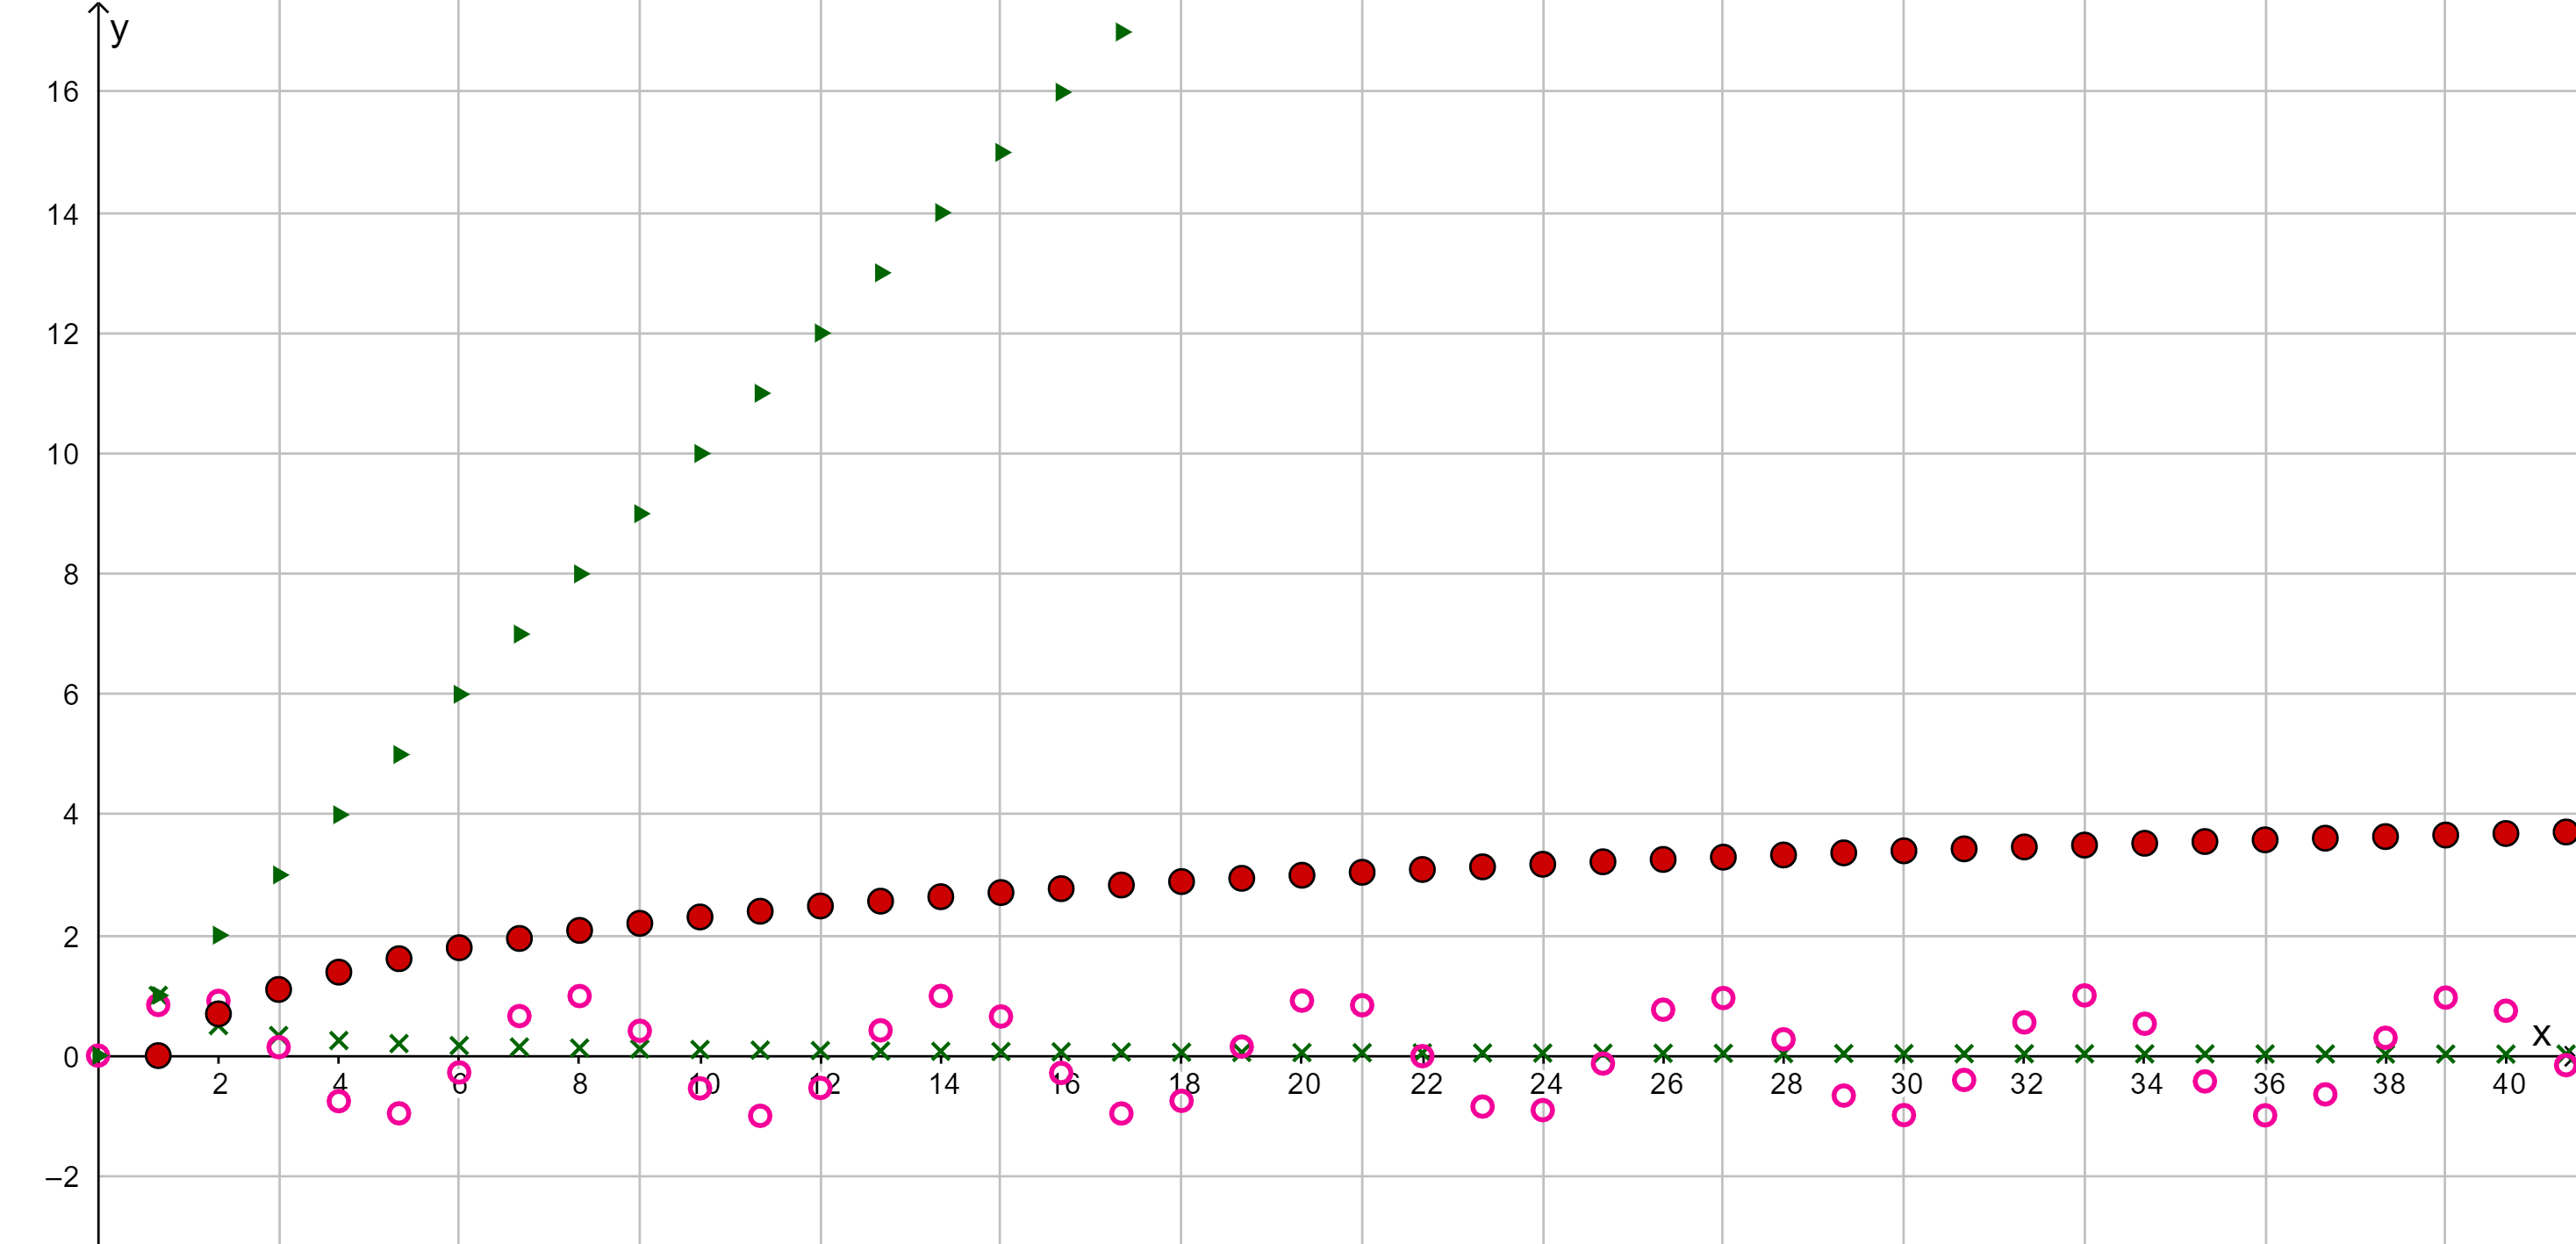
\includegraphics[width=\textwidth]
    {../Mathematik_1/Bilder/folgen_vergleich_eigenschaften.png}
  \end{minipage}
  \begin{minipage}{0.5\textwidth}
    Die dargestellten Folgen unterscheiden sich beispielsweise hinsichtlich
    folgender Eigenschaften:
    \begin{itemize}
      \item beschr�nkt oder unbeschr�nkt,
      \item wachsend oder fallend,
      \item periodisch,
      \item konstant.
    \end{itemize}
  \end{minipage}
\end{exabox}

F�r die folgenden �berlegungen steht eine andere Frage im Mittelpunkt:
\emph{N�hern sich die Folgenglieder f�r zunehmendes \(n\) immer weiter
einem bestimmten Wert an?}

Ein besonders einfaches Beispiel liefert die Folge
\[
a_n=\frac1n.
\]
Ihre ersten Folgenglieder lauten
\[
1,\quad\frac12,\quad\frac13,\quad\frac14,\quad\ldots
\]
und werden immer kleiner. Kein Folgenglied ist gleich \(0\). Trotzdem
lassen sich die Folgenglieder durch hinreichend gro�es \(n\) beliebig nahe
an \(0\) heranbringen.

Dieses Ann�herungsverhalten beschreibt der
\textbf{Grenzwert} (\emph{limit}). F�r das Beispiel gilt
\[
\lim_{n\to\infty}\frac1n=0.
\]

Allgemein bedeutet
\[
\lim_{n\to\infty}a_n=a
\qquad\text{oder kurz}\qquad
a_n\to a,
\]
dass sich die Folgenglieder \(a_n\) f�r zunehmendes \(n\) beliebig nahe
an den Wert \(a\) ann�hern.

Entscheidend ist dabei nicht, ob der Grenzwert \(a\) von der Folge jemals
erreicht wird. Entscheidend ist, dass die Folgenglieder ab einem
hinreichend gro�en Index beliebig nahe bei \(a\) liegen und anschlie�end
auch dort bleiben.


\subsubsection*{Konvergenz}

Die Vorstellung einer Ann�herung l�sst sich mathematisch pr�zisieren.
Dazu wird um den vermuteten Grenzwert \(a\) eine beliebig kleine Umgebung
betrachtet. Ihre Gr��e wird durch eine Zahl \(\varepsilon>0\) beschrieben.

Konvergenz bedeutet, dass sich f�r jede noch so kleine Wahl von
\(\varepsilon\) ein Index finden l�sst, ab dem alle weiteren
Folgenglieder in dieser Umgebung liegen.

\begin{defbox}{Konvergenz einer Zahlenfolge}{ }
Eine Zahlenfolge \((a_n)_n\) hei�t
\textbf{konvergent} (\emph{convergent}) mit Grenzwert \(a\in\mathbb R\),
wenn
\[
\forall\,\varepsilon>0\;
\exists\,N\in\mathbb N^+\;
\forall\,n\geq N:
\qquad
|a_n-a|<\varepsilon.
\]

In diesem Fall gilt
\[
a_n\to a
\qquad\Longleftrightarrow\qquad
\lim_{n\to\infty}a_n=a.
\]

\begin{center}
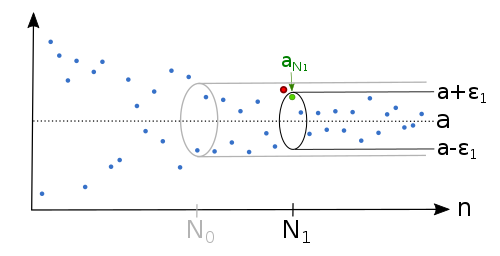
\includegraphics[width=0.55\textwidth]
{../Mathematik_1/Bilder/folgen_konvergenz_epsilon_index.png}
\end{center}
\end{defbox}

Die formale Definition beschreibt genau die zuvor entwickelte
Vorstellung. Die Zahl \(\varepsilon\) gibt einen beliebig kleinen
zul�ssigen Abstand vom Grenzwert \(a\) vor. Zu jedem solchen Abstand
existiert ein Index \(N\). F�r alle \(n\geq N\) gilt dann
\[
|a_n-a|<\varepsilon.
\]
Ab diesem Index liegen also alle weiteren Folgenglieder in der
\(\varepsilon\)-Umgebung des Grenzwerts.

Die Definition dient hier vor allem dazu, die Bedeutung des
Grenzwertbegriffs pr�zise zu erfassen. Grenzwerte werden im Folgenden
nicht durch die direkte Anwendung dieser Definition bestimmt, sondern
mithilfe bekannter Grenzwerte und Grenzwerts�tze.


\begin{exabox}{Ann�herung an einen Grenzwert}{ }
F�r
\[
a_n=\frac{n^2+2}{3n^2}
\]
gilt
\[
a_n
=
\frac{1+\frac{2}{n^2}}{3}.
\]
Da \(2/n^2\) f�r zunehmendes \(n\) gegen \(0\) strebt, n�hern sich die
Folgenglieder dem Wert \(1/3\):
\[
\lim_{n\to\infty}a_n=\frac13.
\]
\end{exabox}


\begin{exabox}{Eine Nullfolge}{ }
F�r die Folge
\[
a_n=\frac3n
\]
gilt
\[
3,\quad\frac32,\quad1,\quad\frac34,\quad\ldots
\longrightarrow0.
\]
Eine Folge mit Grenzwert \(0\) hei�t \textbf{Nullfolge}.
\end{exabox}


\subsubsection*{Konvergenz und Divergenz}

Nicht jede Folge n�hert sich einem festen Wert. Eine Folge, die keinen
endlichen Grenzwert besitzt, hei�t
\textbf{divergent} (\emph{divergent}).

Dabei k�nnen unterschiedliche Formen der Divergenz auftreten. Die Folge
\[
a_n=(-1)^n
\]
wechselt beispielsweise dauerhaft zwischen \(1\) und \(-1\) und n�hert
sich keinem einzelnen Wert.

Eine andere Situation liegt vor, wenn die Folgenglieder schlie�lich �ber
jede vorgegebene Schranke hinauswachsen. In diesem Fall schreibt man
\[
a_n\to\infty.
\]
Entsprechend beschreibt
\[
a_n\to-\infty
\]
eine Folge, deren Werte schlie�lich unter jede vorgegebene Schranke
fallen. Solche Folgen hei�en \textbf{bestimmt divergent}.

\begin{exabox}{Bestimmt divergente Folgen}{ }
\[
n^2\to\infty,
\qquad
e^n\to\infty,
\qquad
\sqrt n\to\infty.
\]
\end{exabox}

Das Symbol \(\infty\) bezeichnet dabei keine reelle Zahl. Eine bestimmt
divergente Folge besitzt daher keinen Grenzwert in \(\mathbb R\).


\noindent\textbf{Bemerkungen:}
\begin{itemize}
  \item Jede konvergente Folge ist beschr�nkt. Die Umkehrung gilt nicht.
  Eine beschr�nkte Folge kann also trotzdem divergent sein.

  \item Monotonie und Beschr�nktheit k�nnen verwendet werden, um
  Konvergenz nachzuweisen. Beispielsweise ist jede nach oben beschr�nkte
  monoton wachsende Folge konvergent. Entsprechend ist jede nach unten
  beschr�nkte monoton fallende Folge konvergent.

  \item Solche Kriterien zum Nachweis von Konvergenz stehen hier nicht im
  Mittelpunkt. Entscheidend ist die Bedeutung des Grenzwerts als
  mathematische Beschreibung eines Ann�herungsprozesses.
\end{itemize}


\begin{exabox}{Beschr�nktheit reicht nicht aus}{ }
  \begin{minipage}{0.5\textwidth}
    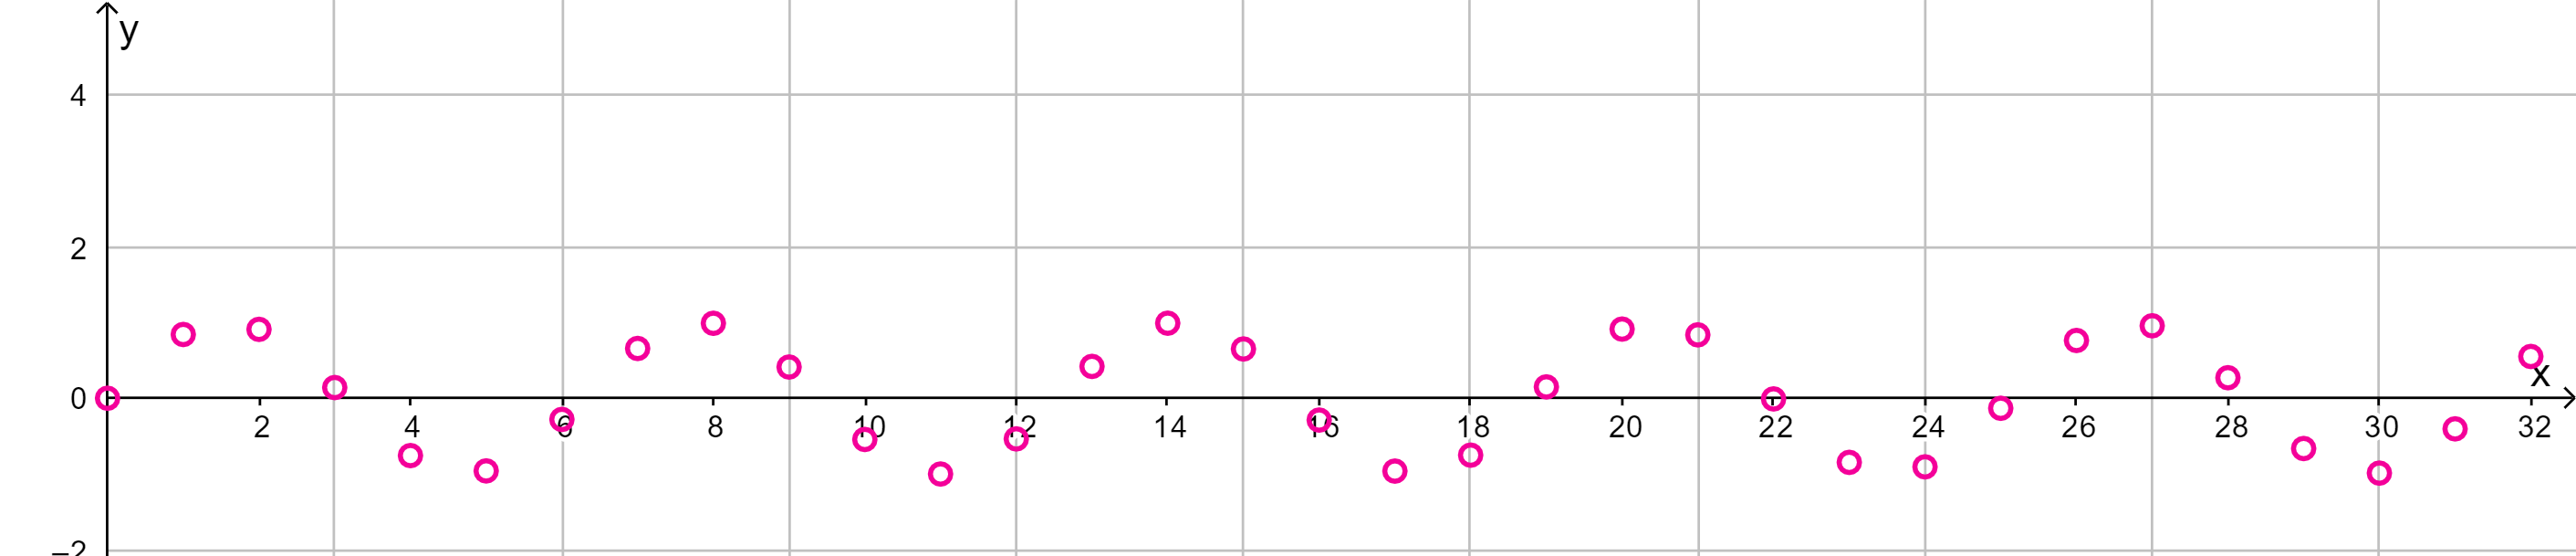
\includegraphics[width=\textwidth]
    {../Mathematik_1/Bilder/folgen_beschraenkt_divergent_oszillation.png}
  \end{minipage}
  \begin{minipage}{0.45\textwidth}
    Eine Folge kann beschr�nkt sein und trotzdem keinen Grenzwert besitzen.
    Beschr�nktheit ist damit notwendig, aber nicht ausreichend f�r
    Konvergenz.
  \end{minipage}
\end{exabox}


\begin{exabox}{Beschr�nktheit und Monotonie}{ }
  \begin{minipage}{0.5\textwidth}
    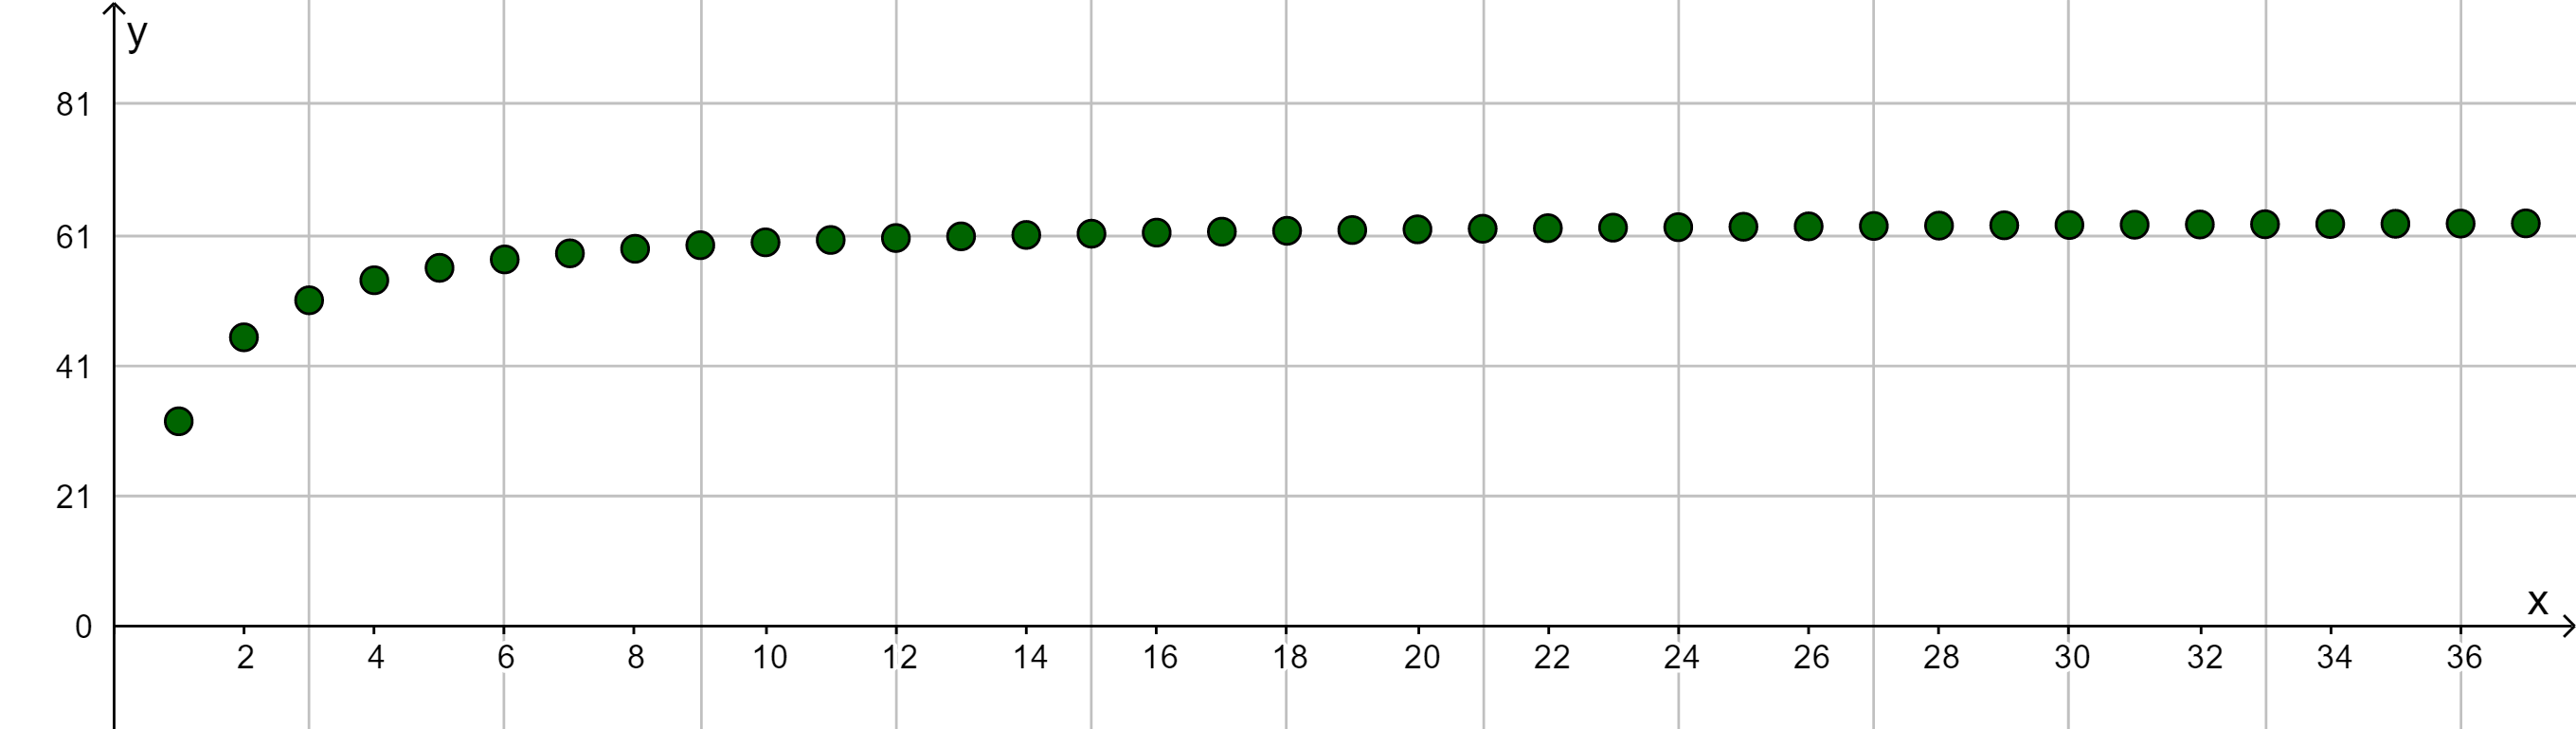
\includegraphics[width=\textwidth]
    {../Mathematik_1/Bilder/folgen_beschraenkt_monoton_konvergent.png}
  \end{minipage}
  \begin{minipage}{0.45\textwidth}
    Eine beschr�nkte monotone Folge ist konvergent. In der dargestellten
    Situation n�hern sich die Folgenglieder einem festen Grenzwert.
  \end{minipage}
\end{exabox}


\subsubsection*{Grenzwerte berechnen}

In praktischen Anwendungen wird ein Grenzwert in der Regel nicht mithilfe
der formalen Definition berechnet. Stattdessen werden bekannte Grenzwerte
und Rechenregeln miteinander kombiniert.

\begin{theorembox}{Grenzwerts�tze f�r Folgen}{ }
Es seien \((a_n)_n\) und \((b_n)_n\) konvergente Zahlenfolgen mit
\[
a_n\to a,
\qquad
b_n\to b.
\]
Dann gilt:
\[
\begin{array}{rcl}
a_n+b_n &\to& a+b,\\[0.5ex]
a_n-b_n &\to& a-b,\\[0.5ex]
a_n\cdot b_n &\to& a\cdot b,\\[0.5ex]
\dfrac{a_n}{b_n} &\to& \dfrac ab
\qquad\textnormal{f�r } b\neq0.
\end{array}
\]

Ist au�erdem \((c_n)_n\) beschr�nkt und gilt
\(|d_n|\to\infty\), so folgt
\[
\frac{c_n}{d_n}\to0.
\]
\end{theorembox}


\begin{exabox}{Ein einfacher Grenzwert}{ }
F�r
\[
a_n=\frac{2n+1}{n}
\]
ergibt sich durch Umformen
\[
\lim_{n\to\infty}\frac{2n+1}{n}
=
\lim_{n\to\infty}\left(2+\frac1n\right)
=
2+0
=
2.
\]
\end{exabox}


\begin{exabox}{Gebrochenrationaler Ausdruck: h�chste Potenz ausklammern}{ }
F�r
\[
\lim_{n\to\infty}
\frac{n^2+\sin(n)}{2n^2+e^{-n}}
\]
wird Z�hler und Nenner durch die h�chste auftretende Potenz \(n^2\)
geteilt:
\[
\lim_{n\to\infty}
\frac{n^2+\sin(n)}{2n^2+e^{-n}}
=
\lim_{n\to\infty}
\frac{1+\frac{\sin(n)}{n^2}}
     {2+\frac{e^{-n}}{n^2}}
=
\frac{1+0}{2+0}
=
\frac12.
\]
Dabei gilt
\[
\left|\frac{\sin(n)}{n^2}\right|
\leq
\frac1{n^2}\to0
\]
und ebenfalls
\[
\frac{e^{-n}}{n^2}\to0.
\]
\end{exabox}


Einige h�ufig auftretende Grenzwerte werden im Folgenden als Referenz
zusammengestellt. Ihre Herleitung steht hier nicht im Mittelpunkt.

\begin{theorembox}{Wichtige Grenzwerte von Folgen}{ }
\begin{itemize}
  \item
  \(\displaystyle
  \lim_{n\to\infty}\left(1+\frac1n\right)^n=e.
  \)

  \item F�r \(a>0\):
  \[
  n^a\to\infty,
  \qquad
  \frac1{n^a}\to0.
  \]

  \item F�r \(|q|<1\) und \(a\in\mathbb R\):
  \[
  q^n\to0,
  \qquad
  n^a q^n\to0.
  \]

  \item F�r \(q>1\) und \(a\in\mathbb R\):
  \[
  q^n\to\infty,
  \qquad
  \frac{q^n}{n^a}\to\infty.
  \]
\end{itemize}
\end{theorembox}


\subsection{Grenzwerte von Funktionen}

Der Grenzwertbegriff f�r Folgen beschreibt einen Ann�herungsprozess:
W�hrend der Index \(n\) immer gr��er wird, k�nnen sich die Folgenglieder
\(a_n\) einem bestimmten Wert ann�hern.

Dieselbe Grundidee l�sst sich auf Funktionen �bertragen. Nun n�hert sich
nicht der Index \(n\) dem Unendlichen, sondern die Variable \(x\) einer
bestimmten Stelle \(x_0\). Im Mittelpunkt steht die Frage, welchem Wert
sich die Funktionswerte \(f(x)\) n�hern, wenn \(x\) beliebig nahe an
\(x_0\) heranr�ckt.

Dabei ist zun�chst nicht entscheidend, welchen Wert die Funktion an der
Stelle \(x_0\) selbst besitzt. Insbesondere kann ein Grenzwert auch dann
existieren, wenn \(f(x_0)\) gar nicht definiert ist.

Der \textbf{Grenzwert einer Funktion} �bertr�gt damit die bereits von
Folgen bekannte Idee der Ann�herung auf das lokale Verhalten einer
Funktion.


\begin{exabox}{Grenzwert an einer Definitionsl�cke}{ }
  \begin{minipage}{0.3\textwidth}
    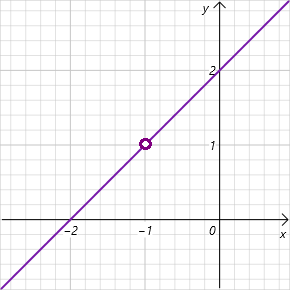
\includegraphics[width=\textwidth]
    {../Mathematik_1/Bilder/grenzwerte_hebbare_definitionsluecke.png}
  \end{minipage}
  \begin{minipage}{0.67\textwidth}
    An der Stelle \(x_0=-1\) ist kein Funktionswert definiert. Die
    Funktionswerte in der Umgebung n�hern sich jedoch von beiden Seiten
    dem Wert \(1\).

    Daher existiert der Grenzwert
    \[
    \lim_{x\to-1}f(x)=1.
    \]

    Die Definitionsl�cke k�nnte durch die Festlegung \(f(-1)=1\)
    geschlossen werden. Im folgenden Abschnitt wird sich zeigen, dass die
    so erg�nzte Funktion an dieser Stelle stetig ist.
  \end{minipage}
\end{exabox}


Der Grenzwert beschreibt somit das Verhalten der Funktion
\emph{in der Umgebung} von \(x_0\), nicht den Funktionswert an \(x_0\)
selbst.

Ein Grenzwert muss allerdings nicht existieren.

\begin{exabox}{Wenn kein Grenzwert existiert}{ }
  \begin{minipage}{0.3\textwidth}
    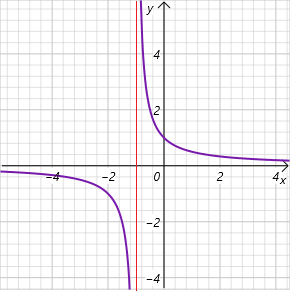
\includegraphics[width=\textwidth]
    {../Mathematik_1/Bilder/grenzwerte_polstelle_vorzeichenwechsel.png}
  \end{minipage}
  \begin{minipage}{0.67\textwidth}
    Bei einer Ann�herung an \(x_0\) zeigen die Funktionswerte von links
    und von rechts kein gemeinsames endliches Verhalten.

    In der dargestellten Situation gilt
    \[
    f(x)\to-\infty
    \quad\textnormal{f�r }x\to x_0^-,
    \]
    w�hrend
    \[
    f(x)\to+\infty
    \quad\textnormal{f�r }x\to x_0^+.
    \]

    Ein gemeinsamer endlicher Grenzwert f�r \(x\to x_0\) existiert daher
    nicht.
  \end{minipage}
\end{exabox}


\subsubsection*{Die pr�zise Bedeutung eines Funktionsgrenzwerts}

Auch beim Funktionsgrenzwert l�sst sich die Vorstellung �beliebig nahe�
mathematisch pr�zisieren.

Die Zahl \(\varepsilon>0\) beschreibt wieder einen beliebig kleinen
Abstand vom Grenzwert \(L\). Nun wird jedoch nicht ein hinreichend gro�er
Index gesucht, sondern eine hinreichend kleine Umgebung der Stelle
\(x_0\). Ihre Gr��e wird durch \(\delta>0\) beschrieben.

\begin{defbox}{Grenzwert einer Funktion}{ }
Sei \(f:D\to\mathbb R\) und \(x_0\) ein H�ufungspunkt von \(D\).
Dann bedeutet
\[
\lim_{x\to x_0}f(x)=L,
\]
dass
\[
\forall\,\varepsilon>0\;
\exists\,\delta>0\;
\forall\,x\in D:
\qquad
0<|x-x_0|<\delta
\Rightarrow
|f(x)-L|<\varepsilon.
\]

\end{defbox}

  \begin{minipage}{0.4\textwidth}
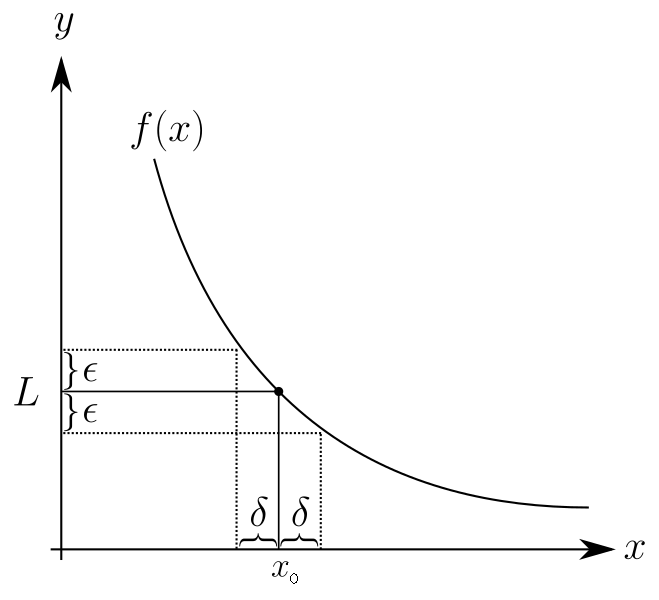
\includegraphics[width=\textwidth]
{../Mathematik_1/Bilder/grenzwerte_definition_epsilon_delta.png}
  \end{minipage}
  \begin{minipage}{0.6\textwidth}
Die Bedingung
\[
0<|x-x_0|<\delta
\]
bedeutet, dass \(x\) hinreichend nahe bei \(x_0\), aber nicht gleich
\(x_0\) liegt. F�r alle solchen \(x\) sollen die zugeh�rigen
Funktionswerte den vorgegebenen Abstand
\[
|f(x)-L|<\varepsilon
\]
vom Grenzwert \(L\) einhalten.

Damit wird auch formal sichtbar, dass der Funktionswert \(f(x_0)\) f�r
die Existenz und den Wert des Grenzwerts zun�chst keine Rolle spielt.
\end{minipage}


\subsubsection*{Die Verbindung zwischen Folgen und Funktionsgrenzwerten}

Die zuvor eingef�hrten Zahlenfolgen erm�glichen eine weitere anschauliche
Interpretation des Funktionsgrenzwerts.

Eine Folge von Stellen
\[
x_1,x_2,x_3,\ldots
\]
kann sich der Stelle \(x_0\) ann�hern:
\[
x_n\to x_0,
\qquad
x_n\neq x_0.
\]
Wird diese Folge in die Funktion eingesetzt, entsteht eine neue Folge
von Funktionswerten
\[
f(x_1),f(x_2),f(x_3),\ldots
\]

Existiert der Funktionsgrenzwert
\[
\lim_{x\to x_0}f(x)=L,
\]
so n�hern sich f�r jede solche Ann�herung an \(x_0\) auch die
Funktionswerte demselben Wert \(L\):
\[
x_n\to x_0
\qquad\Longrightarrow\qquad
f(x_n)\to L.
\]

Damit wird deutlich, weshalb Zahlenfolgen f�r den Grenzwertbegriff von
Funktionen n�tzlich sind: Eine Folge beschreibt einen m�glichen
schrittweisen Weg, sich einer Stelle \(x_0\) zu n�hern. Ein
Funktionsgrenzwert existiert nur dann, wenn das Ergebnis nicht davon
abh�ngt, auf welche Weise diese Ann�herung erfolgt.

F�hren zwei unterschiedliche Ann�herungen an dieselbe Stelle dagegen zu
unterschiedlichen Grenzwerten der Funktionswerte, so kann kein
gemeinsamer Funktionsgrenzwert existieren.


\subsubsection*{Einseitige Grenzwerte}

Bei Funktionen mit reellem Definitionsbereich kann eine Stelle \(x_0\)
von zwei Richtungen angen�hert werden. Eine Ann�herung kann ausschlie�lich
mit Werten \(x<x_0\) oder ausschlie�lich mit Werten \(x>x_0\) erfolgen.

Dies f�hrt zum \textbf{linksseitigen Grenzwert}
\[
\lim_{x\to x_0^-}f(x)
\]
und zum \textbf{rechtsseitigen Grenzwert}
\[
\lim_{x\to x_0^+}f(x).
\]

Ein gemeinsamer Grenzwert
\[
\lim_{x\to x_0}f(x)
\]
existiert genau dann, wenn beide einseitigen Grenzwerte existieren und
�bereinstimmen.

\begin{exabox}{Einseitige Grenzwerte}{ }
  \begin{minipage}{0.3\textwidth}
    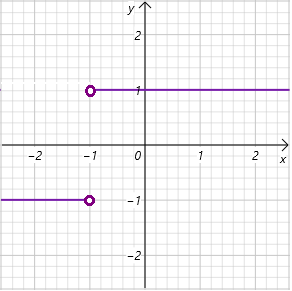
\includegraphics[width=\textwidth]
    {../Mathematik_1/Bilder/grenzwerte_einseitig_sprungstelle.png}
  \end{minipage}
  \begin{minipage}{0.67\textwidth}
    F�r die dargestellte Funktion gilt
    \[
    \lim_{x\to-1^-}f(x)=-1,
    \qquad
    \lim_{x\to-1^+}f(x)=1.
    \]
    Beide einseitigen Grenzwerte existieren, stimmen aber nicht �berein.
    Daher existiert kein gemeinsamer Grenzwert
    \[
    \lim_{x\to-1}f(x).
    \]
  \end{minipage}
\end{exabox}


\noindent\textbf{Bemerkungen:}
\begin{itemize}
  \item F�r einen Grenzwert an einer Stelle \(x_0\) m�ssen Punkte des
  Definitionsbereichs existieren, die beliebig nahe an \(x_0\) liegen
  und von \(x_0\) verschieden sind. Eine solche Stelle hei�t
  \textbf{H�ufungspunkt} des Definitionsbereichs.

  \item An Randpunkten des Definitionsbereichs ist gegebenenfalls nur
  eine einseitige Ann�herung m�glich.

  \item F�r \(x\to\infty\) beziehungsweise \(x\to-\infty\) wird das
  asymptotische Verhalten einer Funktion durch
  \textbf{uneigentliche Grenzwerte} beschrieben.
\end{itemize}


\subsubsection*{Grenzwerte von Funktionen berechnen}

Wie bei Zahlenfolgen werden Grenzwerte von Funktionen in praktischen
Berechnungen normalerweise nicht unmittelbar mithilfe der formalen
Definition bestimmt. Stattdessen werden bekannte Grenzwerte,
Grenzwerts�tze und geeignete Umformungen verwendet.

\begin{theorembox}{Grenzwerts�tze f�r Funktionen}{ }
Seien \(f,g:D\to\mathbb R\) mit
\[
\lim_{x\to x_0}f(x)=a,
\qquad
\lim_{x\to x_0}g(x)=b.
\]
Dann gilt f�r \(c\in\mathbb R\):
\[
\begin{array}{rcl}
\displaystyle
\lim_{x\to x_0}c\,f(x)
&=&ca,\\[1.5ex]

\displaystyle
\lim_{x\to x_0}\bigl(f(x)+g(x)\bigr)
&=&a+b,\\[1.5ex]

\displaystyle
\lim_{x\to x_0}\bigl(f(x)-g(x)\bigr)
&=&a-b,\\[1.5ex]

\displaystyle
\lim_{x\to x_0}f(x)g(x)
&=&ab,\\[1.5ex]

\displaystyle
\lim_{x\to x_0}\frac{f(x)}{g(x)}
&=&\frac ab
\qquad\textnormal{falls }b\neq0.
\end{array}
\]
\end{theorembox}


Besonders einfach ist die Situation bei Funktionen, deren Funktionsterme
an der betrachteten Stelle ohne Problem ausgewertet werden k�nnen.

\begin{exabox}{Direktes Einsetzen}{ }
F�r
\[
f(x)=\frac{x^2+7}{e^x}
\]
ergibt sich an der Stelle \(x_0=2\)
\[
\lim_{x\to2}\frac{x^2+7}{e^x}
=
\frac{2^2+7}{e^2}
=
\frac{11}{e^2}.
\]
\end{exabox}

Interessanter wird der Grenzwert, wenn direktes Einsetzen zun�chst zu
einem unbestimmten Ausdruck f�hrt.

\begin{exabox}{Eine hebbare Definitionsl�cke}{ }
F�r
\[
\lim_{x\to1}\frac{x^2-1}{x-1}
\]
ergibt direktes Einsetzen zun�chst den Ausdruck \(0/0\). Dieser Ausdruck
ist kein Grenzwert und enth�lt f�r sich genommen noch keine Information
�ber das tats�chliche Verhalten der Funktion.

F�r \(x\neq1\) l�sst sich jedoch faktorisieren:
\[
\frac{x^2-1}{x-1}
=
\frac{(x-1)(x+1)}{x-1}
=
x+1.
\]
Da beim Grenzwert \(x=1\) selbst nicht eingesetzt werden muss, folgt
\[
\lim_{x\to1}\frac{x^2-1}{x-1}
=
\lim_{x\to1}(x+1)
=
2.
\]
\end{exabox}

Dieses Beispiel wird f�r die Differentialrechnung von besonderer
Bedeutung sein: Auch bei der Definition der Ableitung entsteht zun�chst
ein Quotient, dessen Z�hler und Nenner gegen \(0\) streben. Der
Grenzwertbegriff erm�glicht es, trotzdem eine wohldefinierte lokale
�nderungsrate zu erhalten.


\begin{exabox}{Ein einseitiger Grenzwert}{ }
F�r
\[
f(x)=\frac{x}{|x|}
\]
gilt f�r \(x<0\)
\[
\frac{x}{|x|}=-1,
\]
w�hrend f�r \(x>0\)
\[
\frac{x}{|x|}=1
\]
gilt. Daher folgen die einseitigen Grenzwerte
\[
\lim_{x\to0^-}\frac{x}{|x|}=-1,
\qquad
\lim_{x\to0^+}\frac{x}{|x|}=1.
\]
Da sie verschieden sind, existiert kein gemeinsamer Grenzwert f�r
\(x\to0\).
\end{exabox}


\subsubsection*{Grenzwerte f�r \(x\to\infty\)}

Grenzwerte werden nicht nur in der Umgebung einer endlichen Stelle
betrachtet. Auch das bereits bekannte asymptotische Verhalten von
Funktionen l�sst sich mit der Grenzwertschreibweise ausdr�cken.

F�r rationale Funktionen
\[
f(x)=\frac{p(x)}{q(x)}
\]
wird das Verhalten f�r gro�e \(|x|\) durch die h�chsten Potenzen in
Z�hler und Nenner bestimmt.

\begin{theorembox}{Grenzwerte rationaler Funktionen f�r \(x\to\infty\)}{ }
Es seien \(p\) und \(q\) Polynome mit Grad \(n\) beziehungsweise \(m\)
und Leitkoeffizienten \(a_n\) beziehungsweise \(b_m\). Dann gilt
\[
\lim_{x\to\infty}\frac{p(x)}{q(x)}
=
\begin{cases}
0, & n<m,\\[1ex]
\dfrac{a_n}{b_m}, & n=m,\\[2ex]
\infty, & n>m\textnormal{ und }a_nb_m>0,\\[1ex]
-\infty, & n>m\textnormal{ und }a_nb_m<0.
\end{cases}
\]
\end{theorembox}

Weitere h�ufig auftretende asymptotische Grenzwerte sind:

\begin{theorembox}{Wichtige Grenzwerte f�r \(x\to\infty\)}{ }
\begin{itemize}
  \item F�r \(a>0\):
  \[
  x^a\to\infty,
  \qquad
  \frac1{x^a}\to0.
  \]

  \item F�r \(0<q<1\) und \(a\in\mathbb R\):
  \[
  q^x\to0,
  \qquad
  q^x x^a\to0.
  \]

  \item F�r \(q>1\) und \(a\in\mathbb R\):
  \[
  \frac{q^x}{x^a}\to\infty.
  \]

  \item F�r \(a>0\):
  \[
  \frac{\ln(x)}{x^a}\to0.
  \]
\end{itemize}
\end{theorembox}


\subsection*{Grenzwerte als Grundlage lokaler Eigenschaften}

Der Grenzwertbegriff erm�glicht es, das Verhalten einer Funktion in der
unmittelbaren Umgebung einer Stelle zu beschreiben. Dabei werden zwei
Gr��en zun�chst bewusst voneinander getrennt:
\[
\lim_{x\to x_0}f(x)
\qquad\textnormal{und}\qquad
f(x_0).
\]

Der erste Ausdruck beschreibt das Verhalten der Funktionswerte
\emph{in der Umgebung} von \(x_0\). Der zweite Ausdruck bezeichnet den
tats�chlichen Funktionswert \emph{an der Stelle} \(x_0\).

Damit entsteht unmittelbar eine neue Frage: Was bedeutet es, wenn beide
Werte �bereinstimmen?

\[
\lim_{x\to x_0}f(x)=f(x_0).
\]

Diese �bereinstimmung f�hrt zum Begriff der
\textbf{Stetigkeit} (\emph{continuity}). Anschaulich bedeutet sie, dass
sich das Verhalten der Funktion in der Umgebung ohne Sprung oder L�cke an
den tats�chlichen Funktionswert anschlie�t.

Der Grenzwertbegriff erm�glicht anschlie�end noch einen weiteren Schritt.
Bei der Differentialrechnung wird untersucht, ob sich nicht nur
Funktionswerte, sondern auch Differenzenquotienten einem festen Wert
ann�hern. Dieser Grenzwert f�hrt zur Ableitung und damit zur lokalen
�nderungsrate einer Funktion.

Grenzwerte bilden damit die begriffliche Grundlage f�r die beiden
zentralen lokalen Eigenschaften der folgenden Abschnitte:
\[
\text{Grenzwert}
\quad\longrightarrow\quad
\text{Stetigkeit}
\quad\longrightarrow\quad
\text{Differenzierbarkeit}.
\]

 % Grenzwerte von Folgen und Funktionen
\newpage
\setcounter{satz}{0} \setcounter{def}{0} \setcounter{exa}{0}  
\section{Stetigkeit und Differenzierbarkeit}\label{MA1-stetigkeit-und-differenzierbarkeit}

\begin{table}[H]
  \centering
  \begin{tabularx}{\textwidth}{p{0.9\textwidth} p{0.1\textwidth}}
    \toprule
    \multicolumn{2}{c}{\textbf{�bersicht �ber Lernziele und Voraussetzungen}}\\
    \midrule
    \textbf{Lernziele} & \\[.5\normalbaselineskip]
    \tabitem Stetigkeit erkl�ren und untersuchen &\\
    \tabitem Parameter so bestimmen, dass eine st�ckweise definierte
    Funktion stetig ist &\\
    \tabitem den Differenzenquotienten als mittlere �nderungsrate interpretieren &\\
    \tabitem die Ableitung als lokale �nderungsrate interpretieren &\\
    \tabitem Differenzierbarkeit �ber den Grenzwert des Differenzenquotienten erkl�ren und untersuchen &\\
    \tabitem den Zusammenhang zwischen Differenzierbarkeit, Stetigkeit und lokaler Linearit�t erl�utern &\\
    \midrule
    \textbf{Voraussetzungen} & \\[.5\normalbaselineskip]
\tabitem Steigung linearer Funktionen & \abschnittsverweis{MA1-eigenschaften-von-funktionen}\\
\tabitem St�ckweise definierte Funktionen & \abschnittsverweis{MA1-eigenschaften-von-funktionen}\\
    \tabitem st�ckweise definierte Funktionen & \abschnittsverweis{MA1-lineare-funktionen}\\
    \tabitem Grenzwerte von Funktionen und einseitige Grenzwerte
    & \abschnittsverweis{MA1-grenzwerte-von-folgen-und-funktionen}\\
    \bottomrule
  \end{tabularx}
\end{table}

\ifintegriereaufgaben
\noindent �bungsaufgaben zum Thema:
\hyperref[MA1-stetigkeit-und-differenzierbarkeit-aufgaben]{Aufgaben}
\vspace{0.3cm}
\hrule
\fi


\subsection{Was ist Stetigkeit?}

Der Grenzwert
\[
\lim_{x\to x_0}f(x)
\]
beschreibt, welchem Wert sich die Funktionswerte n�hern, wenn sich \(x\)
der Stelle \(x_0\) n�hert. Dabei spielt der tats�chliche Funktionswert
\(f(x_0)\) zun�chst keine Rolle.

F�r eine Funktion, die an \(x_0\) definiert ist, k�nnen daher zwei Werte
miteinander verglichen werden:
\[
\lim_{x\to x_0}f(x)
\qquad\textnormal{und}\qquad
f(x_0).
\]

Stimmen beide �berein, so schlie�t sich das Verhalten der Funktion in der
Umgebung von \(x_0\) ohne L�cke oder Sprung an den Funktionswert an.
Genau diese Eigenschaft beschreibt die \textbf{Stetigkeit}
(\emph{continuity}).


\begin{defbox}{Stetigkeit in \(x_0\)}{ }
Eine Funktion \(f:D\to\mathbb R\) ist an einer Stelle \(x_0\in D\)
\textbf{stetig}, wenn
\[
\lim_{x\to x_0}f(x)=f(x_0).
\]
\end{defbox}

F�r Stetigkeit m�ssen damit drei Dinge zusammenpassen: Die Funktion muss
an \(x_0\) definiert sein, der Grenzwert f�r \(x\to x_0\) muss existieren
und dieser Grenzwert muss mit dem Funktionswert \(f(x_0)\) �bereinstimmen.

Anschaulich bedeutet Stetigkeit, dass kleine �nderungen von \(x\) in der
N�he von \(x_0\) nur kleine �nderungen von \(f(x)\) hervorrufen. Der Graph
besitzt dort insbesondere weder einen Sprung noch eine L�cke.


\begin{exabox}{\(\sin:x\mapsto\sin(x)\) ist stetig}{ }
  \begin{minipage}{0.5\textwidth}
    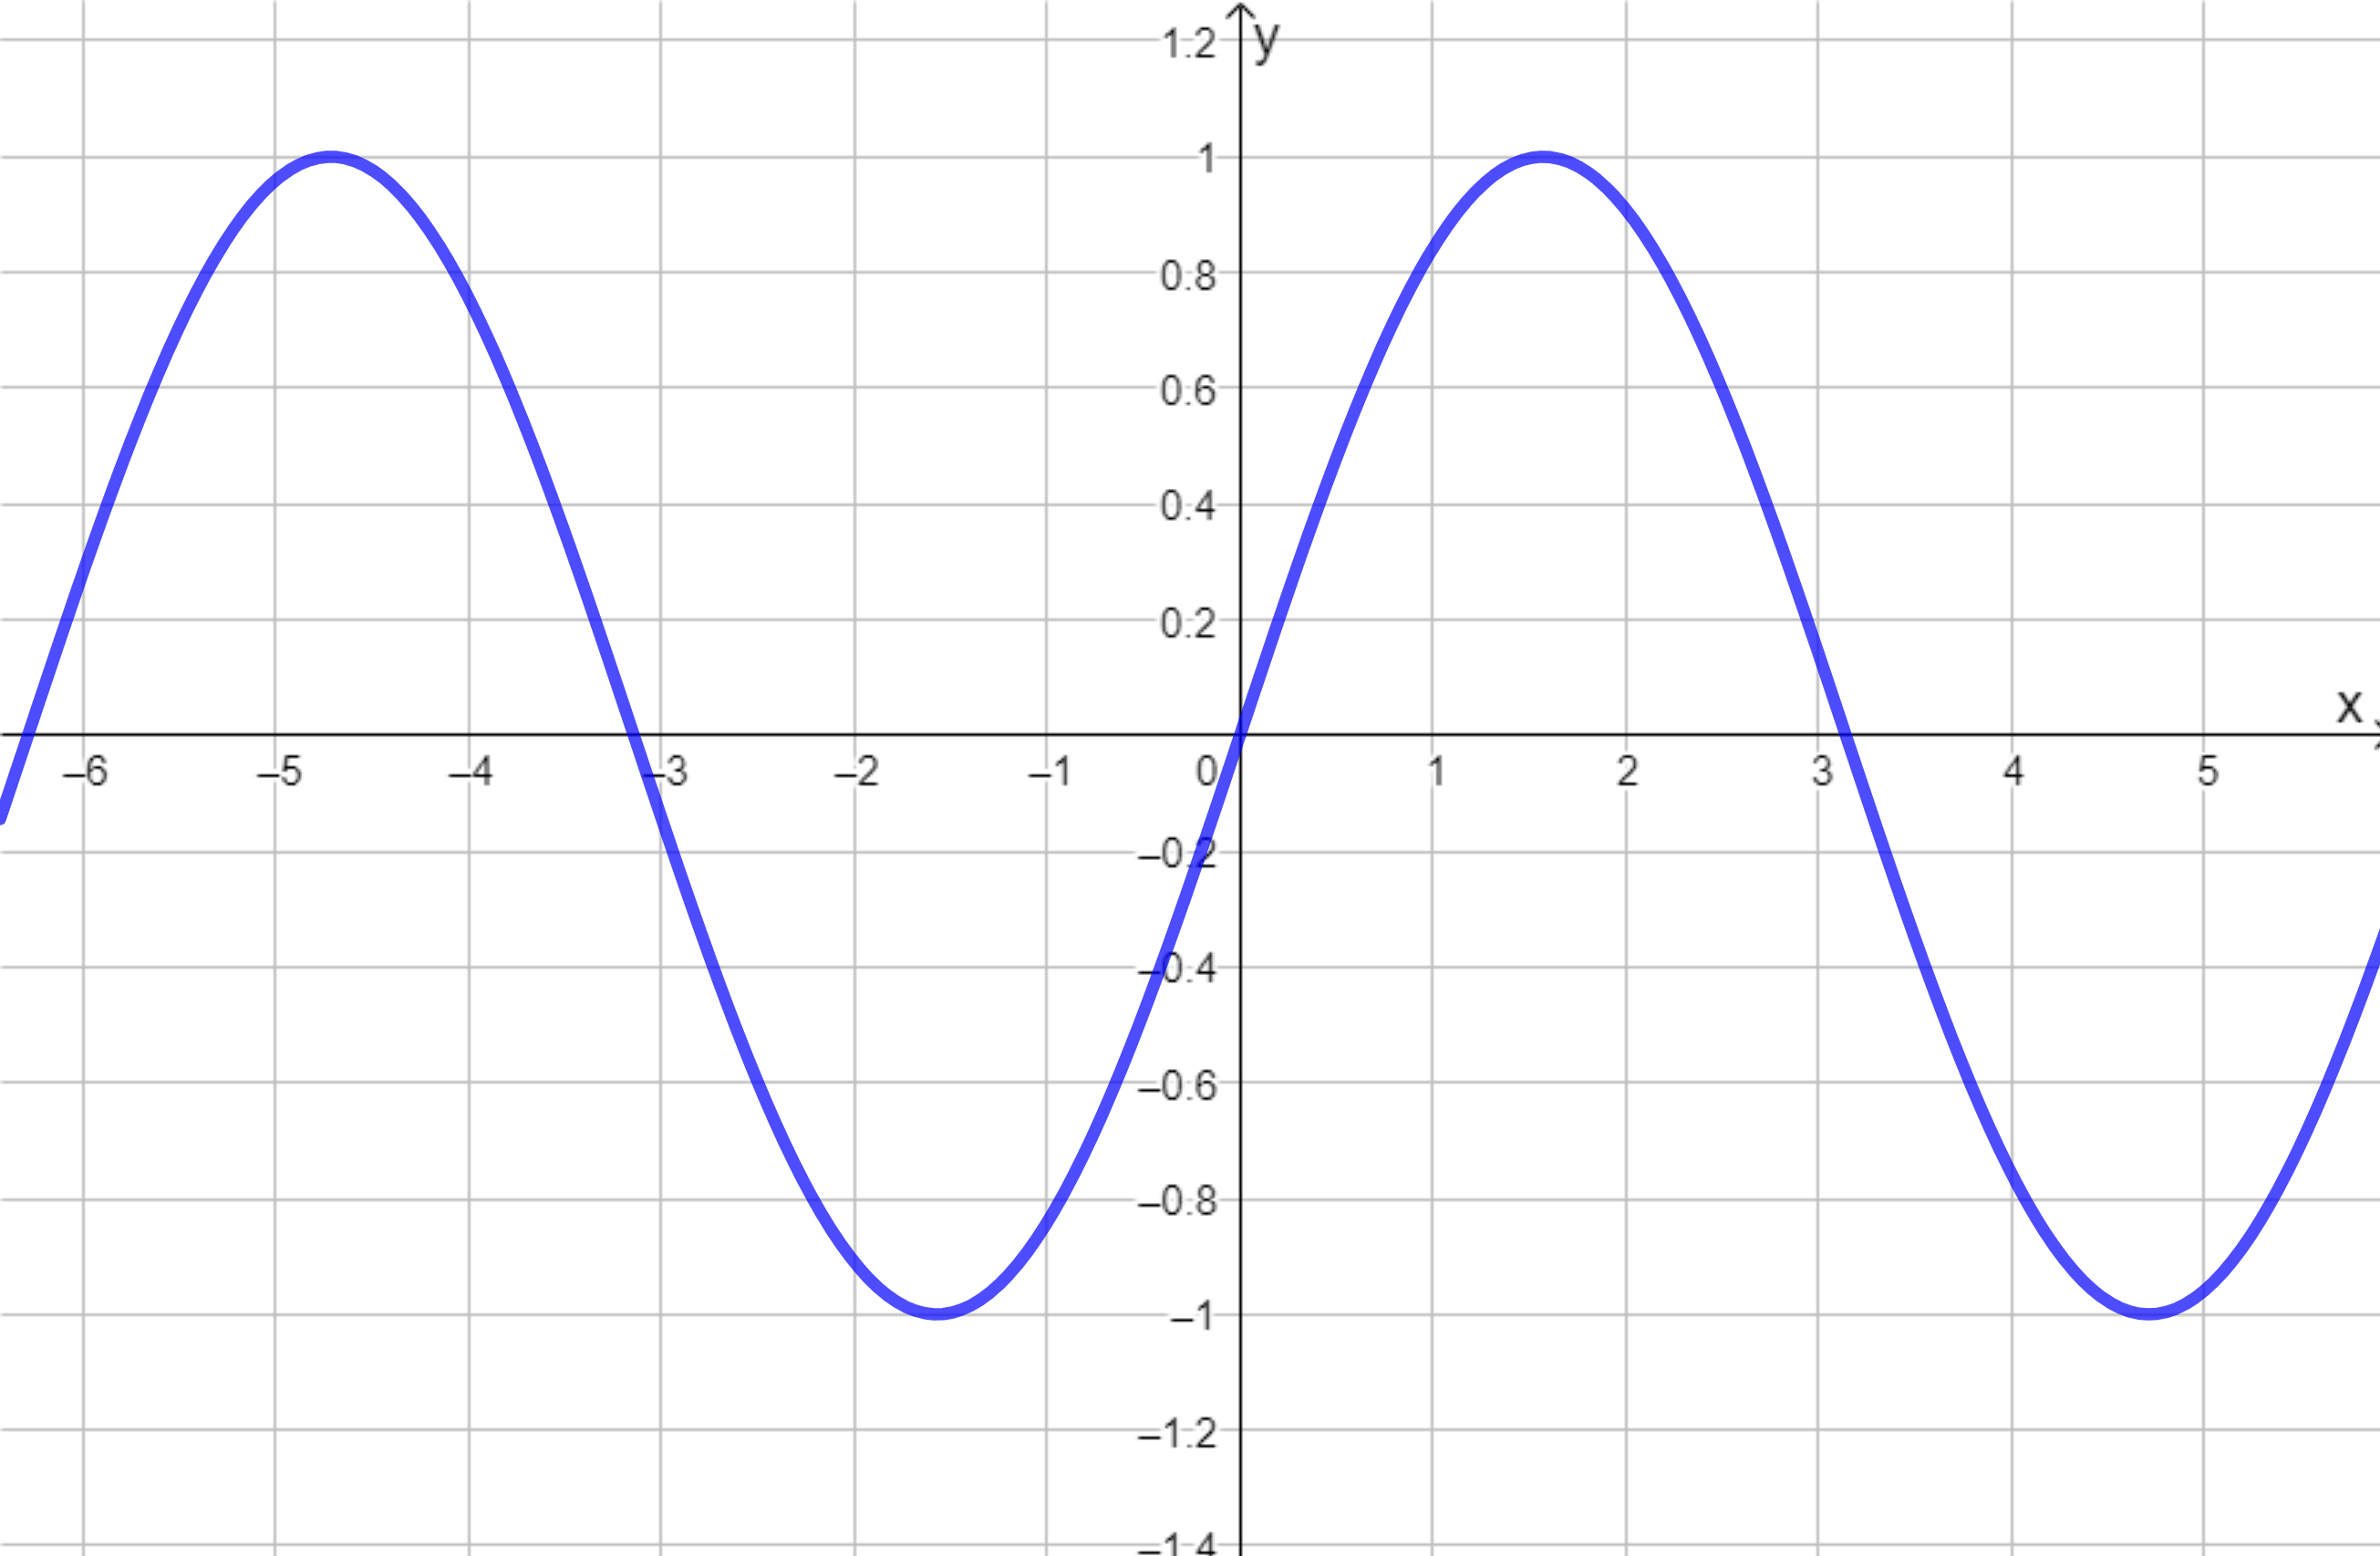
\includegraphics[width=\textwidth]
    {../Mathematik_1/Bilder/stetigkeit_sinusfunktion.png}
  \end{minipage}
  \begin{minipage}{0.45\textwidth}
    Der Graph der Sinusfunktion besitzt weder Spr�nge noch L�cken.

    Anschaulich l�sst er sich zeichnen, ohne den Stift abzusetzen.
    Diese Vorstellung ist f�r viele reelle Funktionen hilfreich, ersetzt
    aber nicht die mathematische Definition der Stetigkeit.
  \end{minipage}
\end{exabox}


\subsubsection*{Eine wichtige Konsequenz der Stetigkeit}

Eine stetige Funktion kann zwischen zwei Funktionswerten keine Werte
�berspringen. Liegen beispielsweise \(f(a)\) und \(f(b)\) auf
unterschiedlichen Seiten eines Wertes \(y\), so muss der Graph den Wert
\(y\) zwischen \(a\) und \(b\) annehmen.

Diese Eigenschaft wird durch den Zwischenwertsatz pr�zisiert.

\begin{theorembox}{Zwischenwertsatz}{ }
Es sei \(f:D\to\mathbb R\) stetig und \([a,b]\subset D\).
F�r jeden Wert \(y\) zwischen \(f(a)\) und \(f(b)\) existiert mindestens
ein \(x\in[a,b]\) mit
\[
f(x)=y.
\]
\end{theorembox}

Eine wichtige Anwendung ergibt sich f�r \(y=0\): Haben \(f(a)\) und
\(f(b)\) unterschiedliche Vorzeichen, so besitzt eine stetige Funktion
zwischen \(a\) und \(b\) mindestens eine Nullstelle.


\subsubsection*{Stetigkeit und Folgen}

Der Grenzwertbegriff wurde zun�chst mithilfe von Zahlenfolgen als
Ann�herungsprozess entwickelt. Auch Stetigkeit l�sst sich in dieser
Vorstellung unmittelbar interpretieren.

N�hert sich eine Folge von Stellen \(x_n\) einer Stelle \(x_0\), so m�ssen
sich bei einer stetigen Funktion die zugeh�rigen Funktionswerte dem
Funktionswert \(f(x_0)\) n�hern.

\begin{theorembox}{Folgenstetigkeit}{ }
Ist \(f\) in \(x_0\) stetig und gilt
\[
x_n\to x_0,
\]
so folgt
\[
f(x_n)\to f(x_0).
\]
\end{theorembox}

Bei stetigen Funktionen kann der Grenzwert damit mit der Funktion
vertauscht werden:
\[
\lim_{n\to\infty}f(x_n)
=
f\left(\lim_{n\to\infty}x_n\right)
=
f(x_0).
\]

In diesem Sinne darf bei stetigen Funktionen der Grenzwert
\emph{eingesetzt} werden.


\subsubsection*{Hebbare Definitionsl�cken}

Der Grenzwert einer Funktion kann an einer Stelle auch dann existieren,
wenn die Funktion dort selbst nicht definiert ist. In diesem Fall ist die
urspr�ngliche Funktion an dieser Stelle nicht stetig, da \(f(x_0)\) nicht
existiert.

Existiert jedoch ein endlicher Grenzwert
\[
\lim_{x\to x_0}f(x)=L,
\]
so kann die fehlende Stelle durch die Festlegung
\[
f(x_0)=L
\]
erg�nzt werden. Eine solche Definitionsl�cke hei�t
\textbf{hebbare Definitionsl�cke}; die erg�nzte Funktion hei�t
\textbf{stetige Fortsetzung}.


\begin{exabox}{Stetige Fortsetzung}{ }
Die Funktion
\[
f:\mathbb R\setminus\{0\}\to(0,\infty),
\qquad
x\mapsto e^{-1/x^2},
\]
ist im Nullpunkt nicht definiert. Es gilt jedoch
\[
\lim_{x\to0}e^{-1/x^2}=0.
\]

Die Definitionsl�cke l�sst sich daher durch den Grenzwert schlie�en.
Eine stetige Fortsetzung ist
\[
\widetilde f:\mathbb R\to[0,\infty),
\qquad
x\mapsto
\begin{cases}
e^{-1/x^2}, & x\neq0,\\
0,          & x=0.
\end{cases}
\]
\end{exabox}


\subsection{Was ist Differenzierbarkeit?}

Stetigkeit beschreibt, ob sich das Verhalten einer Funktion in der
Umgebung einer Stelle ohne Sprung oder L�cke an den dortigen
Funktionswert anschlie�t. F�r die Untersuchung lokaler Ver�nderungen
reicht diese Information jedoch noch nicht aus.

Von besonderem Interesse ist nun die Frage, \emph{wie stark} sich die
Funktionswerte ver�ndern, wenn sich \(x\) in der Umgebung einer Stelle
\(x_0\) ver�ndert.

Dazu werden zun�chst zwei Punkte des Funktionsgraphen betrachtet:
\[
P=\bigl(x_0,f(x_0)\bigr)
\qquad\textnormal{und}\qquad
Q=\bigl(x_0+h,f(x_0+h)\bigr).
\]

Die Gerade durch diese beiden Punkte ist eine Sekante. Ihre Steigung
ergibt sich aus der �nderung der Funktionswerte geteilt durch die �nderung
der Argumente:
\[
\frac{f(x_0+h)-f(x_0)}
     {(x_0+h)-x_0}
=
\frac{f(x_0+h)-f(x_0)}{h}.
\]

Dieser Ausdruck hei�t \textbf{Differenzenquotient}. Er beschreibt die
mittlere �nderungsrate von \(f\) zwischen \(x_0\) und \(x_0+h\).

Nun r�ckt der zweite Punkt immer n�her an den ersten heran. Mathematisch
entspricht dies dem Grenz�bergang
\[
h\to0.
\]
Existiert dabei ein endlicher Grenzwert des Differenzenquotienten, so
entsteht aus der mittleren �nderungsrate eine lokale oder momentane
�nderungsrate. Geometrisch n�hert sich die Sekante einer Tangente an.


\begin{defbox}{Differenzierbarkeit in \(x_0\)}{ }
Eine Funktion \(f\) hei�t an der Stelle \(x_0\)
\textbf{differenzierbar} (\emph{differentiable}), wenn der Grenzwert
\[
\lim_{h\to0}
\frac{f(x_0+h)-f(x_0)}{h}
\]
existiert.

Der Wert dieses Grenzwerts hei�t \textbf{Ableitung}
(\emph{derivative}) von \(f\) an der Stelle \(x_0\):
\[
f'(x_0)
=
\lim_{h\to0}
\frac{f(x_0+h)-f(x_0)}{h}.
\]
\end{defbox}

Die Ableitung \(f'(x_0)\) besitzt damit zwei unmittelbar miteinander
verbundene Interpretationen:

\[
\text{lokale �nderungsrate}
\qquad\longleftrightarrow\qquad
\text{Tangentensteigung}.
\]


\subsubsection*{Die Ableitungsfunktion}

Ist \(f\) nicht nur an einer einzelnen Stelle, sondern an allen Stellen
eines Bereichs differenzierbar, so kann jedem \(x\) die dortige lokale
�nderungsrate zugeordnet werden.

Dadurch entsteht aus \(f\) eine neue Funktion: die
\textbf{Ableitungsfunktion} \(f'\).

\begin{defbox}{Erste Ableitung von \(f\)}{ }
\[
f':
x\mapsto
\lim_{h\to0}
\frac{f(x+h)-f(x)}{h}.
\]

G�ngige Bezeichnungen f�r die erste Ableitung sind
\[
f',
\qquad
\frac{\mathrm df}{\mathrm dx},
\qquad
f^{(1)}.
\]

Ist die unabh�ngige Variable die Zeit \(t\), wird h�ufig auch die
Schreibweise
\[
\dot f=\frac{\mathrm df}{\mathrm dt}
\]
verwendet.
\end{defbox}

Der Definitionsbereich von \(f'\) besteht aus denjenigen Stellen des
Definitionsbereichs von \(f\), an denen \(f\) differenzierbar ist.


\begin{exabox}{Zusammenhang zwischen Funktion und Ableitung}{ }
  \begin{minipage}{0.5\textwidth}
    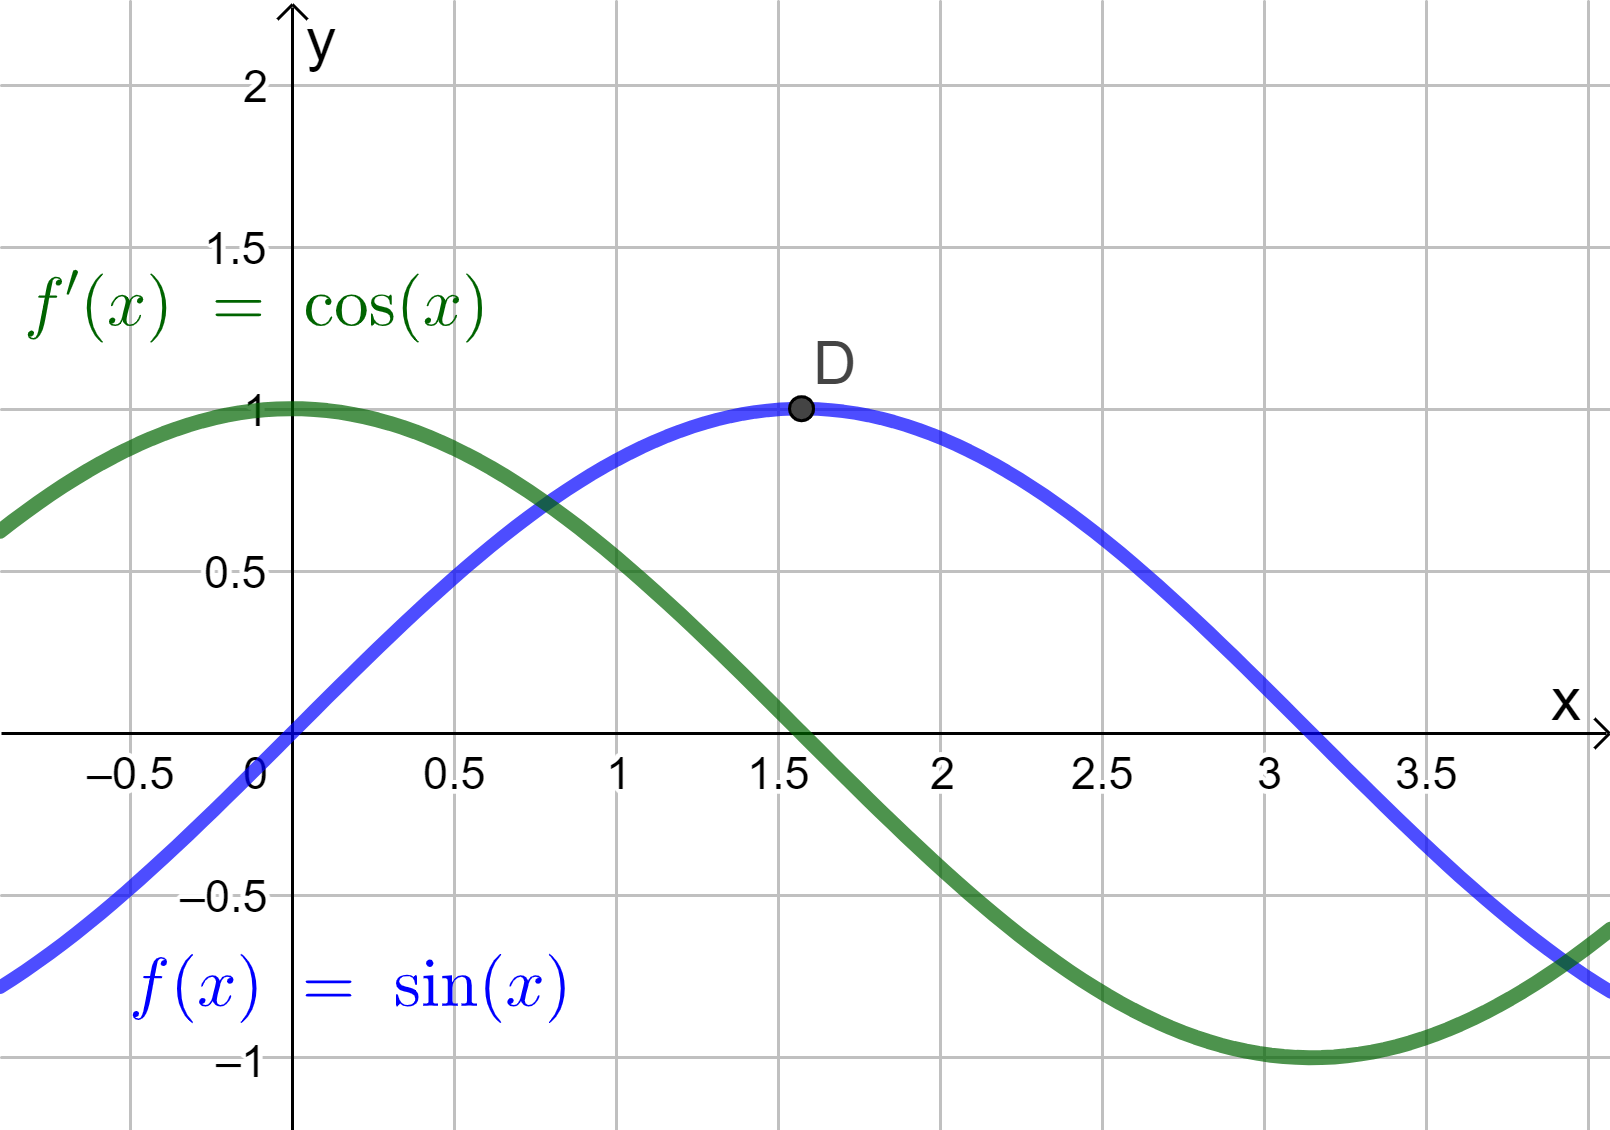
\includegraphics[width=\textwidth]
    {../Mathematik_1/Bilder/ableitung_sinus_kosinus.png}
  \end{minipage}
  \begin{minipage}{0.45\textwidth}
    Die Ableitung beschreibt die lokale �nderung von \(f\):
    \begin{itemize}
      \item W�chst \(f\), so ist \(f'\) positiv.
      \item F�llt \(f\), so ist \(f'\) negativ.
      \item Besitzt \(f\) an einer inneren Stelle ein lokales Maximum oder
      Minimum und ist dort differenzierbar, so gilt \(f'(x)=0\).
    \end{itemize}
  \end{minipage}
\end{exabox}


\subsubsection*{Differenzierbarkeit und Stetigkeit}

Differenzierbarkeit stellt eine st�rkere lokale Anforderung an eine
Funktion als Stetigkeit.

\begin{theorembox}{Differenzierbarkeit und Stetigkeit}{ }
Ist eine Funktion \(f\) an einer Stelle \(x_0\) differenzierbar, so ist
sie dort auch stetig:
\[
f\textnormal{ differenzierbar in }x_0
\quad\Longrightarrow\quad
f\textnormal{ stetig in }x_0.
\]

Die Umkehrung gilt im Allgemeinen nicht.
\end{theorembox}

Eine stetige Funktion kann also durchaus Stellen besitzen, an denen keine
eindeutige Tangentensteigung existiert. Ein besonders einfaches Beispiel
ist die Betragsfunktion.


\begin{exabox}{Stetig, aber nicht differenzierbar: \(f(x)=|x|\)}{ }
  \begin{minipage}{0.5\textwidth}
    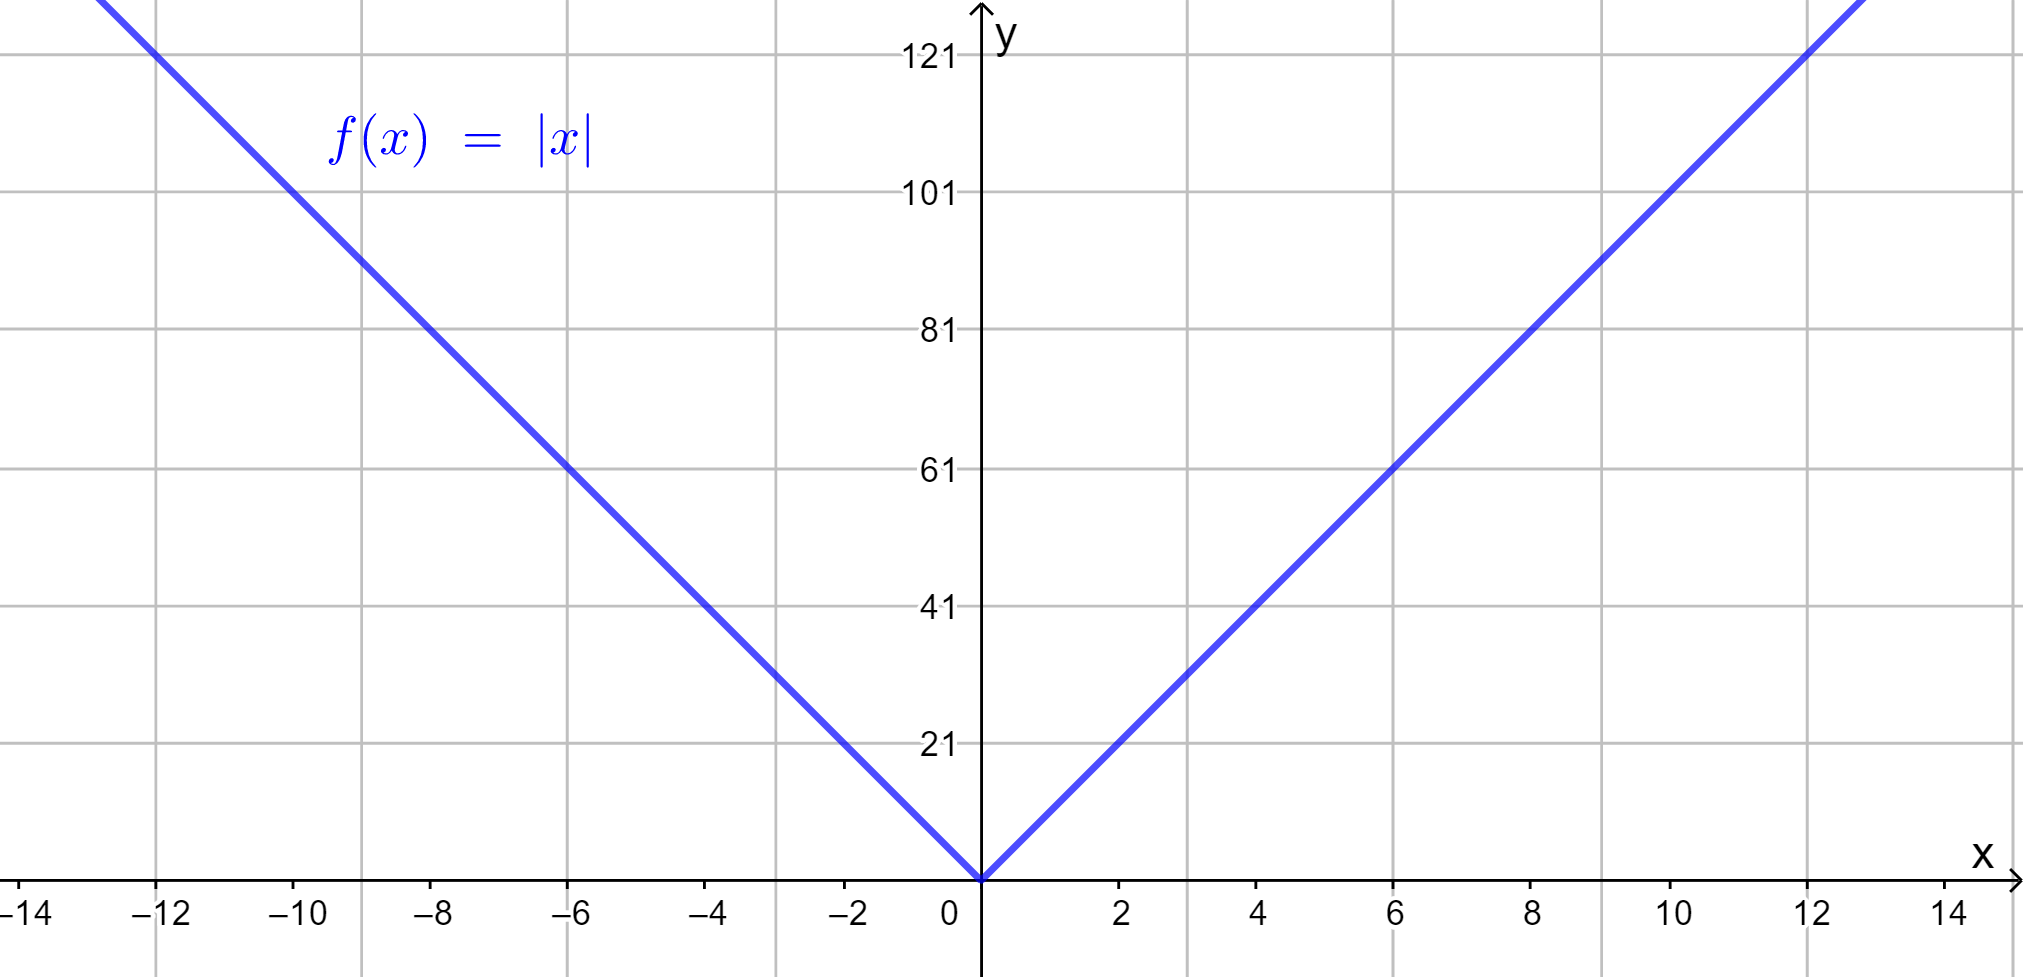
\includegraphics[width=\textwidth]
    {../Mathematik_1/Bilder/differenzierbarkeit_betragsfunktion_knick.png}
  \end{minipage}
  \begin{minipage}{0.45\textwidth}
    Die Betragsfunktion ist in \(x_0=0\) stetig. Dort besitzt ihr Graph
    jedoch einen Knick.

    F�r \(x_0=0\) lautet der Differenzenquotient
    \[
    \frac{f(0+h)-f(0)}{h}
    =
    \frac{|h|}{h}.
    \]

    Die einseitigen Grenzwerte sind
    \[
    \lim_{h\to0^-}\frac{|h|}{h}=-1,
    \qquad
    \lim_{h\to0^+}\frac{|h|}{h}=1.
    \]

    Da beide Grenzwerte verschieden sind, existiert der Grenzwert des
    Differenzenquotienten nicht. Die Betragsfunktion ist daher in
    \(x_0=0\) nicht differenzierbar.
  \end{minipage}
\end{exabox}

Das Beispiel zeigt den Unterschied zwischen beiden Begriffen besonders
deutlich: F�r Stetigkeit gen�gt es, dass sich die Funktionswerte passend
an \(f(x_0)\) anschlie�en. Differenzierbarkeit verlangt zus�tzlich, dass
sich die lokalen �nderungsraten von beiden Seiten an denselben Wert
ann�hern.


\subsection{Differenzierbarkeit als lokale Linearit�t}

Die Ableitung beschreibt nicht nur eine Steigung. Hinter der
Differenzierbarkeit steht eine weitergehende lokale Eigenschaft, die f�r
die folgenden Abschnitte von zentraler Bedeutung ist.

Ist eine Funktion in \(x_0\) differenzierbar, so l�sst sie sich in einer
hinreichend kleinen Umgebung von \(x_0\) immer besser durch eine Gerade
approximieren. Diese Eigenschaft wird als
\textbf{lokale Linearit�t} bezeichnet.

Ausgehend von \(x_0\) wird eine kleine �nderung \(h\) betrachtet. Die
zugeh�rige �nderung des Funktionswertes l�sst sich zerlegen in einen
linearen Anteil
\[
f'(x_0)h
\]
und einen verbleibenden Fehler. Differenzierbarkeit bedeutet, dass dieser
Fehler f�r \(h\to0\) gegen�ber \(h\) vernachl�ssigbar klein wird.


\begin{defbox}{Differenzierbarkeit als lokale Linearisierung}{ }
Eine Funktion \(f\) ist in \(x_0\) genau dann differenzierbar, wenn
\[
f(x_0+h)
=
f(x_0)+f'(x_0)h+r(h),
\]
wobei f�r den Rest \(r(h)\) gilt
\[
\lim_{h\to0}\frac{r(h)}{h}=0.
\]
\end{defbox}

H�ufig wird f�r einen solchen Rest auch die
\textbf{Landau-Schreibweise}
\[
r(h)=o(h)
\]
verwendet. Damit l�sst sich dieselbe Aussage kompakt als
\[
f(x_0+h)
=
f(x_0)+f'(x_0)h+o(h)
\]
schreiben.

Der entscheidende Teil dieser Darstellung ist
\[
f(x_0)+f'(x_0)h.
\]
Er beschreibt die lokale affine Approximation der Funktion.

Mit
\[
h=x-x_0
\]
ergibt sich daraus
\[
f(x)
\approx
f(x_0)+f'(x_0)(x-x_0).
\]

Die zugeh�rige Tangente an den Funktionsgraphen besitzt daher die
Gleichung
\[
t(x)
=
f(x_0)+f'(x_0)(x-x_0).
\]

Die Tangente stimmt an der Stelle \(x_0\) sowohl im Funktionswert als auch
in der Steigung mit \(f\) �berein:
\[
t(x_0)=f(x_0),
\qquad
t'(x_0)=f'(x_0).
\]

Differenzierbarkeit kann damit auf zwei eng miteinander verbundenen Wegen
verstanden werden: �ber den Grenzwert des Differenzenquotienten als
\emph{lokale �nderungsrate} und �ber die Tangente als
\emph{lokale affine Approximation} der Funktion.

Im folgenden Abschnitt werden aus dieser Definition Rechenregeln
entwickelt, mit denen Ableitungen bestimmt werden k�nnen, ohne den
Differenzenquotienten jedes Mal erneut von Grund auf untersuchen zu
m�ssen.
 % Statigkeit und Differenzierbarkeit
\newpage
\setcounter{satz}{0} \setcounter{def}{0} \setcounter{exa}{0}  \section{Ableitungsregeln}\label{MA1-ableitungsregeln}

\begin{table}[H]
  \centering
  \begin{tabularx}{\textwidth}{p{0.9\textwidth} p{0.1\textwidth}}
    \toprule
    \multicolumn{2}{c}{\textbf{�bersicht �ber Lernziele und Voraussetzungen}}\\
    \midrule
    \textbf{Lernziele} & \\[.5\normalbaselineskip]
    \tabitem Ableitungen elementarer Funktionen bestimmen &\\
    \tabitem Summen-, Produkt-, Quotienten- und Kettenregel sicher anwenden &\\
    \tabitem Ableitungen verschachtelter Funktionen systematisch bestimmen &\\
\tabitem die Bedeutung der Exponentialfunktion f�r proportionale �nderungsprozesse erkl�ren (+)&\\
    \midrule
    \textbf{Voraussetzungen} & \\[.5\normalbaselineskip]
    \tabitem Grenzwerte von Funktionen & \abschnittsverweis{MA1-grenzwerte-von-folgen-und-funktionen}\\
    \tabitem Ableitung als lokale �nderungsrate und lokale Linearisierung
    & \abschnittsverweis{MA1-stetigkeit-und-differenzierbarkeit}\\
    \tabitem Verkettung von Funktionen & \abschnittsverweis{MA1-verkettung-von-funktionen}\\
    \bottomrule
  \end{tabularx}
\end{table}

\ifintegriereaufgaben
\noindent �bungsaufgaben zum Thema:
\hyperref[MA1-ableitungsregeln-aufgaben]{Aufgaben}
\vspace{0.3cm}
\hrule
\fi


\subsection{Vom Differenzenquotienten zu Ableitungsregeln}

Die Ableitung wurde im vorigen Abschnitt �ber den Grenzwert des
Differenzenquotienten definiert:
\[
f'(x)
=
\lim_{h\to0}
\frac{f(x+h)-f(x)}{h}.
\]

Diese Definition erkl�rt, \emph{was} eine Ableitung ist: Sie beschreibt
die lokale �nderungsrate einer Funktion und damit die Steigung ihrer
Tangente.

F�r praktische Berechnungen w�re es jedoch aufwendig, f�r jede Funktion
den Differenzenquotienten erneut von Grund auf zu untersuchen. Stattdessen
werden Ableitungen einiger elementarer Funktionen einmal bestimmt und
anschlie�end mithilfe von \textbf{Ableitungsregeln} kombiniert.

Die zentrale Idee ist dabei dieselbe wie bei Funktionstermen selbst:
Komplizierte Funktionen entstehen h�ufig aus einfachen Funktionen durch
Addition, Multiplikation, Division oder Verkettung. Die Struktur des
Funktionsterms bestimmt deshalb, welche Ableitungsregel ben�tigt wird.

So entsteht ein Werkzeugkasten:
\[
\begin{array}{c}
\text{elementare Funktionen}\\
\downarrow\\
\text{Standardableitungen}
\end{array}
\qquad+\qquad
\begin{array}{c}
\text{Verkn�pfungen von Funktionen}\\
\downarrow\\
\text{Ableitungsregeln}.
\end{array}
\]

Die Regeln werden zun�chst f�r die Anwendung zusammengestellt. Ihre
Herleitungen aus der lokalen Linearisierung beziehungsweise aus der
Definition der Ableitung stehen im \textbf{(+)-Teil} am Ende dieses
Abschnitts.


\subsection{Ableitungsregeln}

\subsubsection*{Summen und skalare Vielfache}

Addition und Multiplikation mit einer festen Zahl �bertragen sich besonders
einfach auf die Ableitung.

Sind \(f\) und \(g\) differenzierbar und ist \(C\in\mathbb R\) konstant,
so folgen aus den Grenzwerts�tzen:

\begin{theorembox}{Summenregel und skalare Vielfache}{ }
\[
\begin{array}{rcl}
(Cf)' &=& C f',\\[0.5ex]
(f+g)' &=& f'+g'.
\end{array}
\]
\end{theorembox}

Insbesondere k�nnen Polynome dadurch gliedweise abgeleitet werden, sobald
die Ableitung der Potenzfunktionen bekannt ist.


\subsubsection*{Produkte}

Bei einem Produkt zweier Funktionen reicht es dagegen nicht aus, beide
Faktoren getrennt abzuleiten und anschlie�end zu multiplizieren. �ndern
sich beide Faktoren, so tragen beide �nderungen zur �nderung des Produkts
bei.

\begin{theorembox}{Produktregel}{ }
Sind \(f\) und \(g\) differenzierbar, so gilt
\[
(fg)'
=
f'g+fg'.
\]
\end{theorembox}

Die Struktur der Formel l�sst sich bereits an einem Rechteck
veranschaulichen: �ndern sich beide Seitenl�ngen, so ver�ndert sich die
Fl�che durch die �nderung beider Seiten.

\begin{exabox}{Produktregel geometrisch interpretiert}{ }
\centering
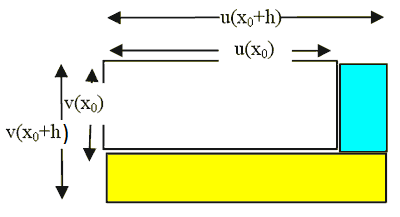
\includegraphics[width=0.5\textwidth]
{../Mathematik_1/Bilder/ableitung_produktregel_flaechenzerlegung.png}
\end{exabox}


\subsubsection*{Verkettungen}

Besonders h�ufig entstehen Funktionen dadurch, dass das Ergebnis einer
Funktion als Argument einer weiteren Funktion verwendet wird:
\[
x\longmapsto g(x)\longmapsto f(g(x)).
\]

Eine kleine �nderung von \(x\) ver�ndert zun�chst den Wert von \(g\).
Diese �nderung wird anschlie�end durch \(f\) weiterverarbeitet. Die
gesamte lokale �nderungsrate entsteht deshalb aus beiden lokalen
�nderungsraten.

\begin{theorembox}{Kettenregel}{ }
Ist \(g\) in \(x\) und \(f\) in \(g(x)\) differenzierbar, so gilt
\[
(f\circ g)'(x)
=
f'(g(x))\,g'(x).
\]
Kurz:
\[
(f\circ g)'=(f'\circ g)\,g'.
\]
\end{theorembox}

Die Kettenregel ist besonders wichtig, weil viele in Anwendungen
auftretende Funktionen Verkettungen elementarer Funktionen sind.

\begin{exabox}{Kettenregel}{ }
F�r
\[
F(x)=e^{-2x}
\]
besteht die Funktion aus der �u�eren Funktion
\[
f(u)=e^u
\]
und der inneren Funktion
\[
g(x)=-2x.
\]
Damit folgt
\[
F'(x)
=
e^{-2x}\cdot(-2)
=
-2e^{-2x}.
\]
\end{exabox}


\subsubsection*{Quotienten}

Ein Quotient kann als Produkt mit dem Kehrwert aufgefasst werden. Aus
Produkt- und Kettenregel ergibt sich dadurch die Quotientenregel.

\begin{theorembox}{Quotientenregel}{ }
Sind \(f\) und \(g\) differenzierbar und gilt \(g(x)\neq0\), so ist
\[
\left(\frac fg\right)'(x)
=
\frac{f'(x)g(x)-f(x)g'(x)}
     {(g(x))^2}.
\]
\end{theorembox}


\subsection{Standardableitungen}

Die Ableitungsregeln beschreiben, wie sich bereits bekannte Ableitungen
kombinieren lassen. Zus�tzlich werden daher die Ableitungen einiger
elementarer Funktionen ben�tigt.

Die folgende �bersicht bildet zusammen mit den Ableitungsregeln den
grundlegenden Werkzeugkasten f�r die folgenden Rechnungen.

\begin{theorembox}{Standardableitungen}{ }
\[
\begin{array}{rcl}
(C)' &=& 0,\\[0.5ex]
(x^n)' &=& nx^{n-1},
\qquad n\in\mathbb N,\\[0.5ex]
(e^x)' &=& e^x,\\[0.5ex]
(b^x)' &=& \ln(b)b^x,
\qquad b>0,\\[0.5ex]
(\ln x)' &=& \displaystyle\frac1x,
\qquad x>0,\\[1ex]
(\sin x)' &=& \cos x,\\
(\cos x)' &=& -\sin x,\\
(\tan x)' &=& \displaystyle\frac1{\cos^2x},\\[1ex]
(\arcsin x)' &=&
\displaystyle\frac1{\sqrt{1-x^2}},
\qquad -1<x<1,\\
(\arccos x)' &=&
-\displaystyle\frac1{\sqrt{1-x^2}},
\qquad -1<x<1,\\
(\arctan x)' &=&
\displaystyle\frac1{1+x^2}.
\end{array}
\]
\end{theorembox}

Die Herleitungen ausgew�hlter Standardableitungen stehen im
\textbf{(+)-Teil}. Dort wird insbesondere sichtbar, wie die bekannten
Eigenschaften von Exponential-, Logarithmus- und trigonometrischen
Funktionen mit ihren Ableitungen zusammenh�ngen.


\subsection{Zusammengesetzte Funktionen systematisch ableiten}

Bei komplizierteren Funktionstermen besteht die eigentliche Aufgabe h�ufig
nicht in der Durchf�hrung einer einzelnen Ableitungsregel, sondern im
Erkennen der Struktur des Terms.

Beispielsweise besitzt
\[
	F(x)=3\cdot e^{-(2\cdot x+1)^2}
\]
vier Ebenen:

\[
x
\longmapsto
2\cdot x + 1
\longmapsto
-(2\cdot x + 1)^2
\longmapsto
e^{-(2\cdot x + 1)^2}
\longmapsto
3 \cdot e^{-(2\cdot x + 1)^2} .
\]

Die Ableitung wird entsprechend von au�en nach innen aufgebaut. 

\begin{exabox}{Zusammengesetzte Funktion}{ }
F�r
\[
	F(x)=3\cdot e^{-(2\cdot x+1)^2}
\]
gilt
\[
F'(x)
=
3\cdot e^{-(2\cdot x+1)^2}\cdot(-2\cdot (2\cdot x+1))\cdot 2
=
- 12 \cdot (2\cdot x+1) \cdot e^{-(2\cdot x+1)^2}.
\]
\end{exabox}

Bei st�rker verschachtelten Termen wird dieses Prinzip wiederholt. Die
�u�ere Struktur entscheidet �ber die zuerst anzuwendende Regel; innere
Funktionen werden anschlie�end auf dieselbe Weise weiter zerlegt.

\subsection{Exponentialfunktionen und proportionale �nderung}
\label{MA1-ableitungsregeln-exponentialfunktion}

Die Exponentialfunktion besitzt eine f�r viele Anwendungen besonders
wichtige Eigenschaft: Ihre Ableitung ist wieder eine Exponentialfunktion.

F�r \(a>0\) gilt
\[
\frac{\mathrm d}{\mathrm dx}a^x
=
\ln(a)\,a^x.
\]

Die Ableitung ist also proportional zum Funktionswert. F�r
\(f(x)=a^x\) gilt
\[
f'(x)=\ln(a)\,f(x).
\]

Damit l�sst sich eine einfache Faustregel formulieren:

\medskip
\noindent
\textbf{Faustregel:}
Immer wenn die momentane �nderungsrate einer Gr��e proportional zu ihrem
aktuellen Wert ist, ist eine Exponentialfunktion zu erwarten.
\medskip

Ein typisches Modell hat daher die Form
\[
y'(t)=\lambda y(t).
\]
Dabei beschreibt \(y(t)\) den aktuellen Wert der betrachteten Gr��e und
\(y'(t)\) ihre momentane �nderungsrate. Der Faktor \(\lambda\) gibt an,
wie gro� die �nderungsrate im Verh�ltnis zum aktuellen Wert ist.

Ein typisches Modell hat daher die Form
\[
y'(t)=\lambda y(t).
\]
Dabei beschreibt \(y(t)\) den aktuellen Wert der betrachteten Gr��e und
\(y'(t)\) ihre momentane �nderungsrate. Der Faktor \(\lambda\) gibt an,
wie gro� die �nderungsrate im Verh�ltnis zum aktuellen Wert ist.

Die L�sungen dieser Gleichung sind genau die Funktionen
\[
y(t)=Ce^{\lambda t},
\qquad C\in\mathbb R.
\]
Tats�chlich gilt
\[
y'(t)
=
\lambda Ce^{\lambda t}
=
\lambda y(t).
\]

F�r \(\lambda>0\) w�chst die Gr��e, f�r \(\lambda<0\) nimmt sie ab.
Je gr��er dabei der aktuelle Betrag von \(y(t)\) ist, desto gr��er ist
auch der Betrag ihrer momentanen �nderung.


\begin{exabox}{Proportionales Wachstum}{}
Eine Gr��e \(y(t)\) erf�lle
\[
y'(t)=y(t),
\qquad
y(0)=y_0.
\]
Die �nderungsrate ist hier zu jedem Zeitpunkt gleich dem aktuellen Wert.
Die Funktion
\[
y(t)=y_0e^t
\]
besitzt genau diese Eigenschaft, denn
\[
y'(t)=y_0e^t=y(t)
\]
und \(y(0)=y_0\).
\end{exabox}

\subsubsection*{Die nat�rliche Exponentialfunktion}

F�r die nat�rliche Exponentialfunktion ist der Proportionalit�tsfaktor
gleich eins:
\[
\left(e^x\right)'=e^x.
\]

Funktionswert und momentane �nderungsrate stimmen daher bei \(e^x\)
�berein. Diese Eigenschaft erkl�rt, weshalb die nat�rliche
Exponentialfunktion bei der Beschreibung von Wachstums- und
Zerfallsprozessen eine besondere Rolle spielt.


\noindent\textbf{Ausblick (+):}
Die Verbindung zwischen Exponentialfunktionen und �nderungsprozessen wird
sp�ter bei Differentialgleichungen wieder aufgegriffen. Eine komplexe
Exponentialfunktion der Form
\[
e^{(\sigma+i\omega)t}
=
e^{\sigma t}\,e^{i\omega t}
\]
verbindet dabei zwei grundlegende Verhaltensweisen: Der reelle Faktor
\(e^{\sigma t}\) beschreibt Wachstum oder D�mpfung. Wegen
\[
e^{i\omega t}
=
\cos(\omega t)+i\sin(\omega t)
\]
beschreibt der zweite Faktor eine Schwingung.

\subsection{Herleitungen und Beweisideen (+)}

Die bisher zusammengestellten Regeln reichen aus, um Ableitungen
praktisch zu berechnen. Ihre Herleitungen zeigen zus�tzlich, weshalb
diese Regeln gelten und wie sie mit der Definition der Ableitung und der
lokalen Linearisierung zusammenh�ngen.

Dieser Teil ist f�r die Anwendung der Regeln nicht erforderlich, macht
aber die gemeinsame mathematische Struktur sichtbar.


\subsubsection*{Herleitung der Produktregel}

Sind \(f\) und \(g\) in \(x\) differenzierbar, so besitzen beide eine
lokale Linearisierung:
\[
f(x+h)
=
f(x)+f'(x)h+o(h)
\]
und
\[
g(x+h)
=
g(x)+g'(x)h+o(h).
\]

F�r das Produkt ergibt sich damit
\begin{eqnarray*}
f(x+h)g(x+h)
&=&
\left(f(x)+f'(x)h+o(h)\right)
\left(g(x)+g'(x)h+o(h)\right)\\[1ex]
&=&
f(x)g(x)
+
\left(f'(x)g(x)+f(x)g'(x)\right)h
+
o(h).
\end{eqnarray*}

Der lineare Anteil der �nderung besitzt somit den Koeffizienten
\[
f'(x)g(x)+f(x)g'(x).
\]
Nach der Charakterisierung der Differenzierbarkeit durch lokale
Linearisierung ist genau dieser Koeffizient die Ableitung des Produkts.

\begin{theorembox}{Produktregel}{ }
\[
(fg)'
=
f'g+fg'.
\]
\end{theorembox}


\subsubsection*{Herleitung der Kettenregel}

Nun wird die Verkettung
\[
x\mapsto f(g(x))
\]
betrachtet. Die Funktion \(g\) sei in \(x\) differenzierbar und \(f\) in
\(g(x)\).

F�r die innere Funktion gilt
\[
g(x+h)
=
g(x)+g'(x)h+o(h).
\]
Die �nderung des Arguments der �u�eren Funktion ist daher
\[
h_2
:=
g(x+h)-g(x)
=
g'(x)h+o(h).
\]

Da auch \(f\) differenzierbar ist, gilt
\[
f(g(x)+h_2)
=
f(g(x))+f'(g(x))h_2+o(h_2).
\]

Einsetzen von \(h_2\) liefert
\[
f(g(x+h))
=
f(g(x))
+
f'(g(x))g'(x)h
+
o(h).
\]

Der lineare Koeffizient ist somit
\[
f'(g(x))g'(x).
\]

\begin{theorembox}{Kettenregel}{ }
\[
(f\circ g)'(x)
=
f'(g(x))g'(x).
\]
\end{theorembox}

Die Kettenregel macht damit mathematisch pr�zise, was bereits bei ihrer
Einf�hrung anschaulich sichtbar war: Eine kleine �nderung von \(x\) wird
zun�chst durch \(g\) und anschlie�end durch \(f\) weitergegeben. Die
beiden lokalen �nderungsfaktoren multiplizieren sich.


\subsubsection*{Herleitung der Quotientenregel}

Zun�chst wird die Ableitung der Kehrwertfunktion betrachtet. Aus
\[
x\cdot\frac1x=1
\]
folgt mit der Produktregel
\[
0
=
\left(x\cdot\frac1x\right)'
=
\frac1x
+
x\left(\frac1x\right)'.
\]
Damit gilt
\[
\left(\frac1x\right)'
=
-\frac1{x^2}.
\]

F�r eine differenzierbare Funktion \(g\) folgt mit der Kettenregel
\[
\left(\frac1{g(x)}\right)'
=
-\frac{g'(x)}{(g(x))^2}.
\]

Schlie�lich wird
\[
\frac{f(x)}{g(x)}
=
f(x)\frac1{g(x)}
\]
als Produkt aufgefasst. Die Produktregel ergibt
\[
\left(\frac fg\right)'
=
\frac{f'g-fg'}{g^2}.
\]


\subsubsection*{Herleitungen ausgew�hlter Standardableitungen}

\paragraph{Exponentialfunktion.}

Aus dem \underline{bekannten Grenzwert}\randverweis{MA1-grenzwerte-von-folgen-und-funktionen}
\[
\lim_{h\to0}\frac{e^h-1}{h}=1
\]
folgt unmittelbar
\begin{eqnarray*}
\frac{e^{x+h}-e^x}{h}
&=&
e^x\frac{e^h-1}{h}.
\end{eqnarray*}
Damit ergibt sich f�r \(h\to0\)
\[
(e^x)'=e^x.
\]
Damit ergibt sich f�r \(h\to0\)
\[
(e^x)'=e^x.
\]

\begin{theorembox}{Ableitung der Exponentialfunktion}{ }
\[
\exp'=\exp.
\]
\end{theorembox}

F�r eine beliebige Basis \(b>0\) gilt
\[
b^x=e^{x\ln b}.
\]
Mit der Kettenregel folgt
\[
(b^x)'
=
e^{x\ln b}\ln b
=
\ln(b)b^x.
\]


\paragraph{Logarithmusfunktion.}

Exponentialfunktion und nat�rlicher Logarithmus sind Umkehrfunktionen.
F�r \(x>0\) gilt
\[
e^{\ln x}=x.
\]
Ableiten beider Seiten und Anwenden der Kettenregel liefert
\[
e^{\ln x}(\ln x)'=1.
\]
Wegen \(e^{\ln x}=x\) folgt
\[
(\ln x)'=\frac1x.
\]


\paragraph{Potenzfunktionen.}

F�r \(x>0\) l�sst sich
\[
x^n=e^{n\ln x}
\]
schreiben. Mit der Kettenregel folgt
\begin{eqnarray*}
\frac{\mathrm d}{\mathrm dx}x^n
&=&
\frac{\mathrm d}{\mathrm dx}e^{n\ln x}\\
&=&
e^{n\ln x}\frac{n}{x}\\
&=&
nx^{n-1}.
\end{eqnarray*}

F�r \(n\in\mathbb N\) gilt diese Ableitungsregel auf dem gesamten
Definitionsbereich der jeweiligen Potenzfunktion.


\paragraph{Trigonometrische Funktionen.}

Eine besonders kompakte Herleitung ergibt sich mithilfe der Eulerschen
Identit�t
\[
e^{ix}=\cos x+i\sin x.
\]
Ableiten liefert
\[
\frac{\mathrm d}{\mathrm dx}e^{ix}
=
ie^{ix}
=
i(\cos x+i\sin x)
=
-\sin x+i\cos x.
\]

Durch Vergleich von Real- und Imagin�rteil folgt
\[
(\cos x)'=-\sin x,
\qquad
(\sin x)'=\cos x.
\]

F�r den Tangens ergibt sich anschlie�end mit der Quotientenregel
\begin{eqnarray*}
(\tan x)'
&=&
\left(\frac{\sin x}{\cos x}\right)'\\
&=&
\frac{\cos^2x+\sin^2x}{\cos^2x}\\
&=&
\frac1{\cos^2x}.
\end{eqnarray*}


\paragraph{Inverse trigonometrische Funktionen.}

Die Ableitungen der inversen trigonometrischen Funktionen lassen sich
�hnlich wie die Ableitung des Logarithmus aus der Beziehung zwischen
einer Funktion und ihrer Umkehrfunktion gewinnen.

F�r den Arkussinus gilt
\[
\sin(\arcsin x)=x.
\]
Ableiten liefert
\[
\cos(\arcsin x)(\arcsin x)'=1.
\]
Da
\[
\cos(\arcsin x)=\sqrt{1-x^2}
\qquad\textnormal{f�r }-1<x<1,
\]
folgt
\[
(\arcsin x)'
=
\frac1{\sqrt{1-x^2}}.
\]

Entsprechend ergeben sich
\[
(\arccos x)'
=
-\frac1{\sqrt{1-x^2}},
\qquad -1<x<1,
\]
und
\[
(\arctan x)'
=
\frac1{1+x^2}.
\]
 % Ableitungsregeln
\newpage
\setcounter{satz}{0} \setcounter{def}{0} \setcounter{exa}{0}  \section{Lokale Linearit�t}\label{MA1-lokale-linearitaet}

\begin{table}[H]
  \centering
  \begin{tabularx}{\textwidth}{p{0.9\textwidth} p{0.1\textwidth}}
    \toprule
    \multicolumn{2}{c}{\textbf{�bersicht �ber Lernziele und Voraussetzungen}}\\
    \midrule
    \textbf{Lernziele} &\\[.5\normalbaselineskip]
    \tabitem Differenzierbarkeit als lokale Linearit�t interpretieren &\\
    \tabitem eine Funktion durch ihre Tangente lokal approximieren &\\
    \tabitem die Bedeutung der Kr�mmung f�r die Genauigkeit einer
             Linearisierung erkl�ren &\\
    \tabitem die Regel von L'Hospital zur Untersuchung geeigneter
             Grenzwerte anwenden &\\
    \tabitem Ableitungen aus diskreten Funktionswerten durch
             Differenzenquotienten approximieren &\\
    \tabitem das Newton-Verfahren als wiederholte Linearisierung
             erkl�ren und anwenden &\\
    \midrule
    \textbf{Voraussetzungen} &\\[.5\normalbaselineskip]
    \tabitem Grenzwerte von Funktionen verstehen & \abschnittsverweis{MA1-grenzwerte-von-folgen-und-funktionen}\\
    \tabitem Differenzierbarkeit und Ableitung interpretieren & \abschnittsverweis{MA1-stetigkeit-und-differenzierbarkeit}\\
    \tabitem Ableitungen berechnen & \abschnittsverweis{MA1-ableitungsregeln}\\
    \bottomrule
  \end{tabularx}
\end{table}

\ifintegriereaufgaben
\noindent �bungsaufgaben zum Thema:
\hyperref[MA1-lokale-linearitaet-aufgaben]{Aufgaben}
\vspace{0.3cm}
\hrule
\fi


% =========================================================
\subsection{Differenzierbarkeit bedeutet lokale Linearit�t}
\label{MA1-lokale-linearitaet-differenzierbarkeit}

Viele Funktionen, die in Anwendungen auftreten, sind nichtlinear.
Nichtlineare Funktionen und Gleichungen sind im Allgemeinen schwieriger
zu untersuchen als lineare. Die Differenzierbarkeit er�ffnet jedoch einen
grundlegenden Zugang:

\medskip
\noindent
\emph{In hinreichend kleiner Umgebung kann eine differenzierbare Funktion
durch ein lineares Modell ersetzt werden.}
\medskip

Dieses Prinzip hei�t \textbf{Linearisierung} (\emph{linearization}).
Es geh�rt zu den grundlegenden Ideen der Analysis und insbesondere der
Numerik. Statt ein nichtlineares Problem unmittelbar zu behandeln, wird
es zun�chst lokal durch ein einfacheres lineares Problem ersetzt.

Ist \(f\) in \(x_0\) differenzierbar, so ist die Tangente
\[
T_{x_0}(x)
=
f(x_0)+f'(x_0)(x-x_0)
\]
die lokale affine Approximation der Funktion.

F�r \(x=x_0+h\) ergibt sich entsprechend
\[
T_{x_0}(x_0+h)
=
f(x_0)+f'(x_0)h.
\]

Die Aussage, dass die Tangente die Funktion lokal approximiert, l�sst sich
pr�zise formulieren.

\begin{theorembox}{Lokale Linearit�t}{}
Ist \(f\) in \(x_0\) differenzierbar, so gilt
\[
f(x_0+h)
=
f(x_0)+f'(x_0)h+r(h),
\]
wobei
\[
\lim_{h\to0}\frac{r(h)}{h}=0.
\]
\end{theorembox}

Der Rest \(r(h)\) verschwindet also f�r \(h\to0\) schneller als die
Schrittweite \(h\). In diesem pr�zisen Sinn wird die Funktion in immer
kleinerer Umgebung von \(x_0\) immer besser durch ihre Tangente
beschrieben.

Mit der \textbf{Landau-Schreibweise} l�sst sich die Bedingung an den Rest
kurz als
\[
r(h)=o(h)
\]
schreiben. Damit lautet die lokale Linearisierung
\[
f(x_0+h)
=
f(x_0)+f'(x_0)h+o(h).
\]

Die Ableitung \(f'(x_0)\) ist somit nicht nur eine Tangentensteigung oder
eine lokale �nderungsrate. Sie bestimmt zugleich den linearen Anteil der
lokalen �nderung von \(f\).

Anschaulich:
\[
\text{nahe }x_0:
\qquad
f
\approx
\text{Tangente}.
\]

Diese Idee wird in Mathematik~2 durch Taylor-Polynome erweitert. Dort wird
eine Funktion nicht nur durch einen linearen, sondern durch einen
polynomiellen Ausdruck h�herer Ordnung lokal approximiert.


\begin{exabox}{Lokale Approximation eines Funktionswertes}{}

F�r
\[
f(x)=\sqrt{x}
\]
ist der Funktionswert bei \(x_0=100\) unmittelbar bekannt:
\[
f(100)=10.
\]
Au�erdem gilt
\[
f'(x)=\frac{1}{2\sqrt{x}},
\qquad
f'(100)=\frac1{20}.
\]

Die Linearisierung der Wurzelfunktion bei \(x_0=100\) lautet daher
\[
T_{100}(x)
=
10+\frac1{20}(x-100).
\]

F�r \(x=103\) ergibt sich
\[
\sqrt{103}
\approx
T_{100}(103)
=
10+\frac3{20}
=
10{,}15.
\]

Die nichtlineare Wurzelfunktion wurde damit in der N�he von \(100\) durch
eine affine Funktion ersetzt. Die eigentliche N�herungsrechnung ist
anschlie�end nur noch linear.
\end{exabox}

\noindent\textbf{Bemerkung:}
Linearisierung ist eine lokale Aussage. Je weiter sich \(x\) von der
Entwicklungsstelle \(x_0\) entfernt, desto st�rker kann sich die Funktion
von ihrer Tangente unterscheiden.


% =========================================================
\subsection{Wie gut ist die Linearisierung?}
\label{MA1-lokale-linearitaet-fehlerabschaetzung}

Eine N�herung ist besonders dann n�tzlich, wenn zumindest eingesch�tzt
werden kann, wie gro� ihr Fehler ist.

Die Tangente stimmt an der Stelle \(x_0\) mit der Funktion im Funktionswert
und in der Steigung �berein:
\[
T_{x_0}(x_0)=f(x_0),
\qquad
T_{x_0}'(x_0)=f'(x_0).
\]

Entfernt sich \(x\) von \(x_0\), macht sich jedoch die
\textbf{Kr�mmung} der Funktion bemerkbar. Eine nahezu geradlinig
verlaufende Funktion bleibt �ber einen gr��eren Bereich nahe an ihrer
Tangente; bei starker Kr�mmung verliert die Tangentenapproximation
schneller an Genauigkeit.

Die zweite Ableitung liefert ein Ma� f�r diese Kr�mmung. Damit entsteht
der qualitative Zusammenhang
\[
\text{gro�es }|f''|
\quad\Longrightarrow\quad
\text{st�rkere Abweichung von der Tangente}.
\]

Diese Beobachtung f�hrt zu einer quantitativen Fehlerabsch�tzung.


\subsubsection*{Fehlerabsch�tzung (+)}

Ist \(f\) zweimal stetig differenzierbar und gilt
\[
|f''(x)|\le M
\]
f�r alle \(x\) zwischen \(x_0\) und \(x_0+h\), so l�sst sich der Fehler
der linearen Approximation absch�tzen.

\begin{theorembox}{Fehler der linearen Approximation}{}
Unter den genannten Voraussetzungen gilt
\[
\left|
f(x_0+h)
-
\bigl(f(x_0)+f'(x_0)h\bigr)
\right|
\le
\frac{M}{2}h^2.
\]
\end{theorembox}

Der Fehler ist damit h�chstens von der Gr��enordnung \(h^2\). Wird die
Schrittweite beispielsweise halbiert, so wird dieser Anteil der
Fehlerabsch�tzung um den Faktor vier kleiner.

Die systematische Herleitung dieser Aussage erfolgt sp�ter mithilfe des
Taylor-Satzes. F�r den Moment ist vor allem die Struktur wichtig:
Die erste Ableitung liefert die lineare Approximation, die zweite
Ableitung kontrolliert deren Fehler.


\begin{exabox}{Fehlerabsch�tzung f�r \(\sqrt{103}\)}{}

F�r
\[
f(x)=\sqrt{x}
\]
gilt
\[
f''(x)
=
-\frac{1}{4x^{3/2}}.
\]

Im Intervall \([100,103]\) gilt daher
\[
|f''(x)|
\le
\frac1{4000}.
\]
Mit \(h=3\) folgt
\[
\left|
\sqrt{103}-10{,}15
\right|
\le
\frac12\cdot\frac1{4000}\cdot 3^2
=
\frac9{8000}.
\]

Da \(f''(x)<0\), ist die Wurzelfunktion in diesem Bereich nach unten
gekr�mmt und liegt unterhalb ihrer Tangente. Damit ergibt sich sogar
\[
10{,}15-\frac9{8000}
\le
\sqrt{103}
\le
10{,}15.
\]

Zum Vergleich:
\[
\sqrt{103}=10{,}148891\ldots
\]
\end{exabox}


% =========================================================
\subsection{Grenzwerte durch lokale �nderungsraten:
die Regel von L'Hospital}
\label{MA1-lokale-linearitaet-lhospital}

Die lokale Beschreibung einer Funktion durch ihre Ableitung l�sst sich
auch zur Untersuchung von Grenzwerten nutzen.

Bei einem Quotienten
\[
\frac{f(x)}{g(x)}
\]
kann es vorkommen, dass f�r \(x\to x_0\) sowohl Z�hler als auch Nenner
gegen null streben. Direktes Einsetzen f�hrt dann auf die
\textbf{unbestimmte Form}
\[
\frac00.
\]
Dieser Ausdruck besitzt keinen eigenen Zahlenwert. Er zeigt vielmehr an,
dass aus den Grenzwerten von Z�hler und Nenner allein noch nicht folgt,
wie sich ihr Quotient verh�lt.

Die Idee der Linearisierung liefert zun�chst eine anschauliche Erkl�rung.
Seien beispielsweise
\[
f(x_0)=0,
\qquad
g(x_0)=0.
\]
Dann gilt lokal
\[
f(x_0+h)
=
f'(x_0)h+o(h)
\]
und
\[
g(x_0+h)
=
g'(x_0)h+o(h).
\]

Falls \(g'(x_0)\neq0\), werden Z�hler und Nenner in erster N�herung durch
ihre linearen Anteile beschrieben. Daher verh�lt sich der Quotient f�r
kleine \(h\) wie
\[
\frac{f(x_0+h)}{g(x_0+h)}
\approx
\frac{f'(x_0)h}{g'(x_0)h}
=
\frac{f'(x_0)}{g'(x_0)}.
\]

Die lokalen �nderungsraten k�nnen also dar�ber entscheiden, wie sich der
Quotient zweier gegen null strebender Funktionen verh�lt.

Diese �berlegung erkl�rt einen wichtigen Spezialfall der
\textbf{Regel von L'Hospital} (\emph{L'Hospital's rule}). Der allgemeine
Satz ist weiterreichend und ben�tigt eigene Voraussetzungen.


\begin{theorembox}{Regel von L'Hospital}{}
Es seien \(f\) und \(g\) in einer punktierten Umgebung von \(x_0\)
differenzierbar und es gelte dort \(g'(x)\neq0\). Weiter sei
\[
\lim_{x\to x_0}f(x)
=
\lim_{x\to x_0}g(x)
=
0.
\]

Existiert der Grenzwert
\[
\lim_{x\to x_0}
\frac{f'(x)}{g'(x)}
=
L
\]
als endlicher oder uneigentlicher Grenzwert, so gilt unter diesen
Voraussetzungen
\[
\lim_{x\to x_0}
\frac{f(x)}{g(x)}
=
L.
\]
\end{theorembox}

Eine entsprechende Aussage gilt unter geeigneten Voraussetzungen auch
f�r Quotienten der unbestimmten Form
\[
\frac{\infty}{\infty}.
\]


\begin{exabox}{Regel von L'Hospital}{}

Der Grenzwert
\[
\lim_{x\to0}
\frac{\sin x}{e^x-1}
\]
f�hrt beim direkten Einsetzen auf die unbestimmte Form \(0/0\).

Mit der Regel von L'Hospital folgt
\[
\lim_{x\to0}
\frac{\sin x}{e^x-1}
=
\lim_{x\to0}
\frac{\cos x}{e^x}
=
1.
\]

Die lokale Linearisierung macht das Ergebnis zus�tzlich anschaulich:
F�r kleine \(x\) gilt
\[
\sin x\approx x
\qquad\text{und}\qquad
e^x-1\approx x.
\]
Z�hler und Nenner besitzen bei \(x=0\) also denselben linearen Anteil.
Ihr Quotient n�hert sich deshalb dem Wert \(1\).
\end{exabox}

\noindent\textbf{Bemerkung:}
Die Linearisierung erkl�rt die Grundidee von L'Hospital besonders
anschaulich, wenn die ersten Ableitungen bereits das lokale Verhalten
bestimmen. Der allgemeine Satz ist jedoch nicht lediglich eine
Umformulierung der Tangentenapproximation.


% =========================================================
\subsection{Linearisierung aus diskreten Daten}
\label{MA1-lokale-linearitaet-diskrete-daten}

Bisher wurde die Ableitung als bekannt vorausgesetzt und daraus die
Linearisierung einer Funktion bestimmt. In Messungen, Experimenten und
numerischen Berechnungen tritt h�ufig die umgekehrte Situation auf:

Die Funktionswerte sind bekannt, die Ableitung jedoch nicht.

Beispielsweise kann eine physikalische Gr��e nur zu diskreten Zeitpunkten
gemessen worden sein. Zwischen den Messpunkten liegen dann keine
unmittelbaren Informationen �ber den Funktionsverlauf vor.

Die lokale Linearit�t liefert auch hier die entscheidende Idee. Ist eine
Funktion in einem kleinen Bereich ann�hernd geradlinig, so l�sst sich die
unbekannte Tangentensteigung durch die Steigung einer nahe gelegenen
Sekante approximieren.

F�r zwei benachbarte Funktionswerte ergibt sich beispielsweise
\[
f'(x)
\approx
\frac{f(x+h)-f(x)}{h}.
\]

Damit wird die Ableitung selbst zu einer Gr��e, die numerisch aus
Funktionswerten approximiert werden kann.


\begin{exabox}{Differenzenquotienten}{}
\begin{center}
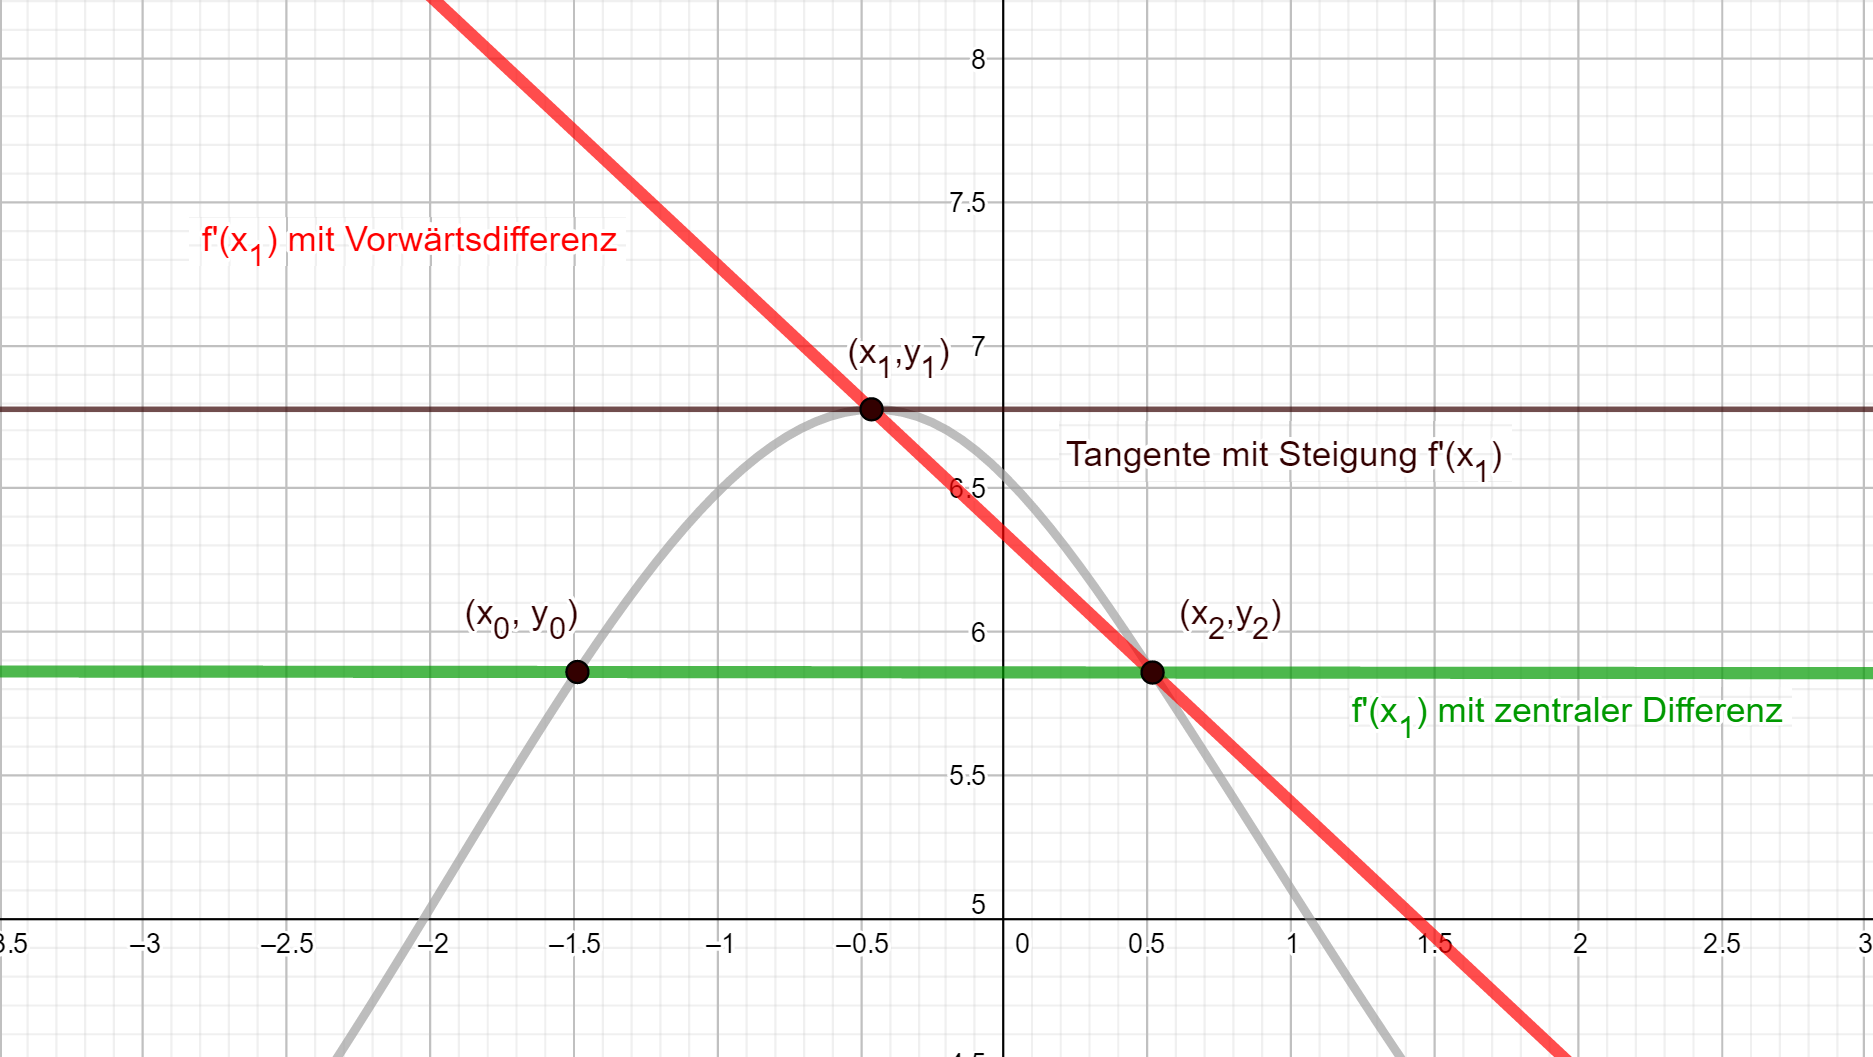
\includegraphics[width=0.8\textwidth]
{../Mathematik_1/Bilder/ableitung_differenzenquotienten_vergleich.png}
\end{center}
\end{exabox}

Werden Funktionswerte auf beiden Seiten der betrachteten Stelle verwendet,
so ergibt sich die \textbf{zentrale Differenz}
(\emph{central difference})
\[
f'(x)
\approx
\frac{f(x+h)-f(x-h)}{2h}.
\]

Geometrisch entspricht dieser Ausdruck wieder einer Sekantensteigung.
Durch die symmetrische Wahl der beiden Punkte heben sich jedoch bestimmte
Fehleranteile gegenseitig auf. Deshalb ist die zentrale Differenz bei
glatten Funktionen typischerweise genauer als die einseitige
Vorw�rtsdifferenz.


\subsubsection*{Genauigkeit von Differenzenquotienten (+)}

F�r hinreichend glatte Funktionen gelten die Fehlerordnungen
\[
\textnormal{Vorw�rtsdifferenz:}
\qquad
f'(x)
=
\frac{f(x+h)-f(x)}{h}
+
\mathcal O(h),
\]
w�hrend f�r die zentrale Differenz
\[
\textnormal{zentrale Differenz:}
\qquad
f'(x)
=
\frac{f(x+h)-f(x-h)}{2h}
+
\mathcal O(h^2)
\]
gilt.

Die zentrale Differenz besitzt damit einen Fehler zweiter Ordnung:
Wird \(h\) halbiert, verkleinert sich dieser Fehleranteil n�herungsweise
um den Faktor vier.

Auch die zweite Ableitung kann aus benachbarten Funktionswerten
approximiert werden:

\begin{theorembox}{Zweite Differenz}{}
F�r hinreichend glatte Funktionen gilt
\[
f''(x)
=
\frac{f(x+h)-2f(x)+f(x-h)}{h^2}
+
\mathcal O(h^2).
\]
\end{theorembox}

Diese Formeln sind erste Beispiele f�r ein grundlegendes Vorgehen der
Numerik: Aus endlich vielen diskreten Daten werden lokale Eigenschaften
einer kontinuierlichen Funktion approximiert.

\noindent\textbf{Bemerkung:}
Mathematisch wird die Approximation f�r kleiner werdendes \(h\) zun�chst
genauer. In tats�chlichen numerischen Rechnungen kann \(h\) jedoch nicht
beliebig klein gew�hlt werden, da Rundungsfehler und Messfehler dann
zunehmend ins Gewicht fallen. Die Wahl einer geeigneten Schrittweite ist
daher selbst Teil eines numerischen Verfahrens.


% =========================================================
\subsection{Newton-Verfahren: wiederholte Linearisierung}
\label{MA1-lokale-linearitaet-newton-verfahren}

Ein besonders wichtiges Beispiel f�r die Nutzung lokaler Linearit�t ist
die numerische L�sung nichtlinearer Gleichungen.

Gesucht sei eine L�sung der Gleichung
\[
f(x)=0.
\]
F�r viele nichtlineare Funktionen l�sst sich eine solche Gleichung nicht
durch einfache algebraische Umformungen l�sen. Das
\textbf{Newton-Verfahren} (\emph{Newton's method}) ersetzt deshalb das
nichtlineare Problem lokal durch ein lineares.

Ausgehend von einem N�herungswert \(x_k\) wird \(f\) in der N�he von
\(x_k\) linearisiert:
\[
f(x)
\approx
f(x_k)+f'(x_k)(x-x_k).
\]

Anstatt unmittelbar eine Nullstelle der nichtlinearen Funktion zu suchen,
wird nun zun�chst die Nullstelle dieser Tangente bestimmt. Dazu wird das
lineare Ersatzproblem
\[
0
=
f(x_k)+f'(x_k)(x-x_k)
\]
gel�st.

F�r \(f'(x_k)\neq0\) folgt
\[
x
=
x_k-\frac{f(x_k)}{f'(x_k)}.
\]

Dieser Wert wird als neuer N�herungswert verwendet:
\[
x_{k+1}
=
x_k-\frac{f(x_k)}{f'(x_k)}.
\]

Anschlie�end wird die Funktion am neuen Punkt \(x_{k+1}\) erneut
linearisiert. Das Verfahren wiederholt somit immer denselben Ablauf:
\[
\text{linearisieren}
\longrightarrow
\text{lineares Problem l�sen}
\longrightarrow
\text{neu linearisieren}.
\]


\begin{defbox}{Newton-Verfahren}{}
Sei \(f\) differenzierbar und \(x_0\) ein geeigneter Startwert. Solange
\(f'(x_k)\neq0\) gilt, wird rekursiv
\[
x_{k+1}
=
x_k-\frac{f(x_k)}{f'(x_k)}
\]
berechnet.
\end{defbox}


\begin{exabox}{Newton-Verfahren: Idee in Bildern}{}
\begin{minipage}{0.32\textwidth}
  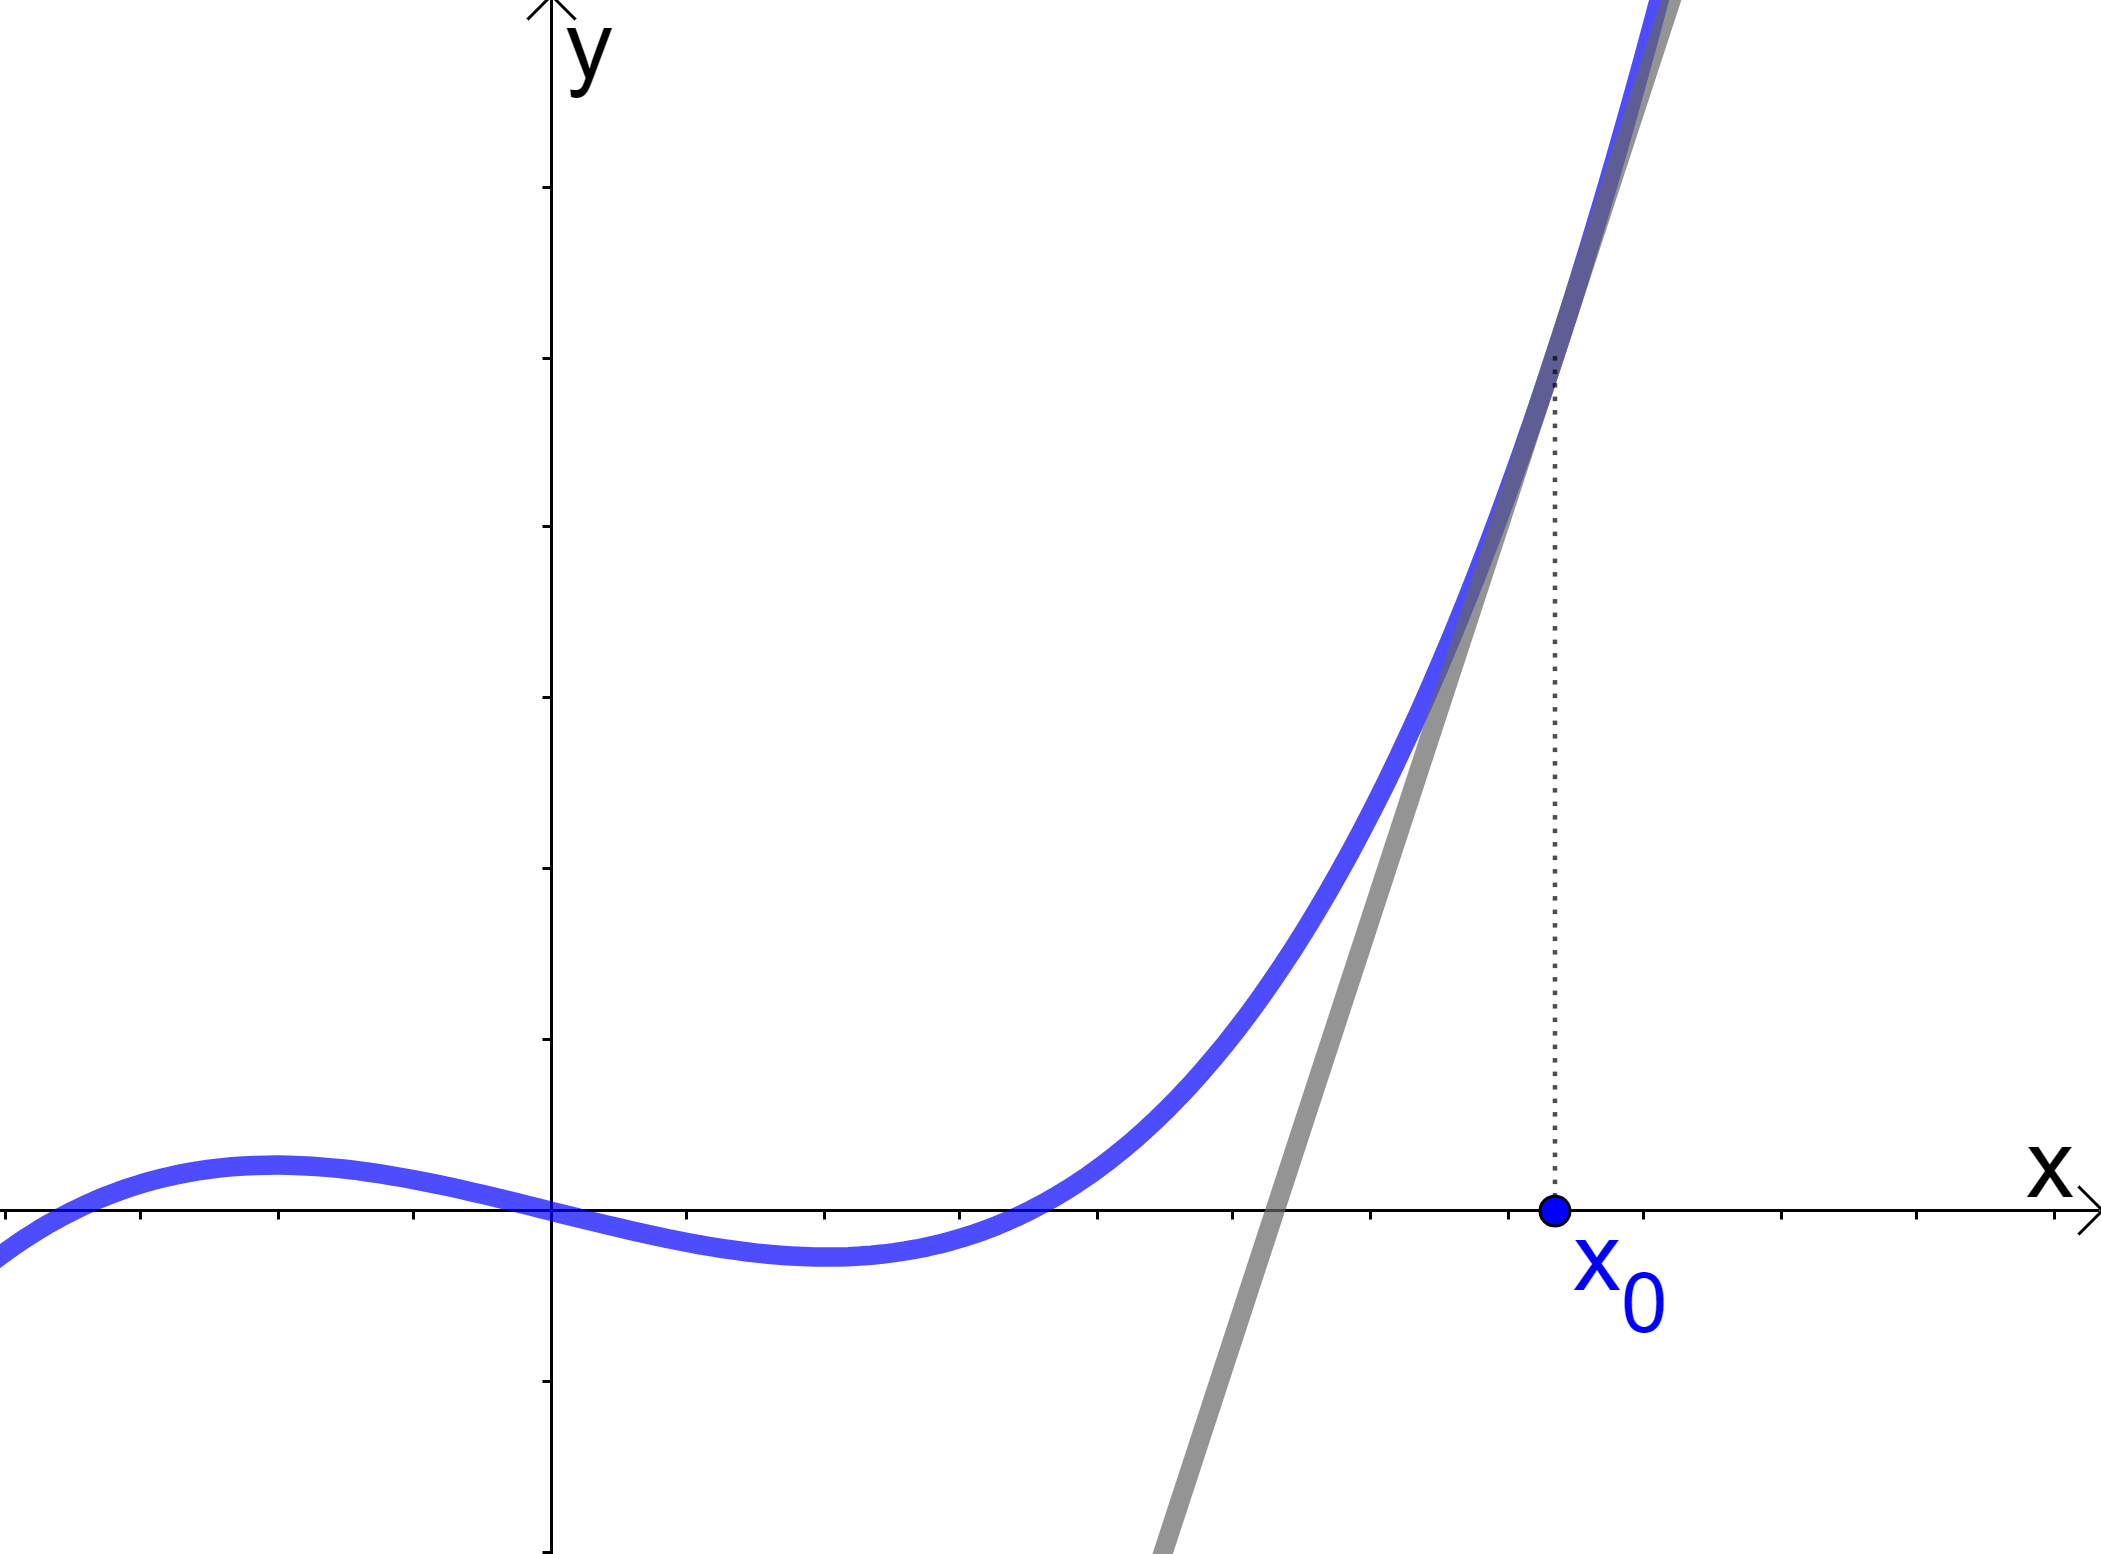
\includegraphics[width=\textwidth]
  {../Mathematik_1/Bilder/newton_tangente_startwert.png}
\end{minipage}\hfill
\begin{minipage}{0.32\textwidth}
  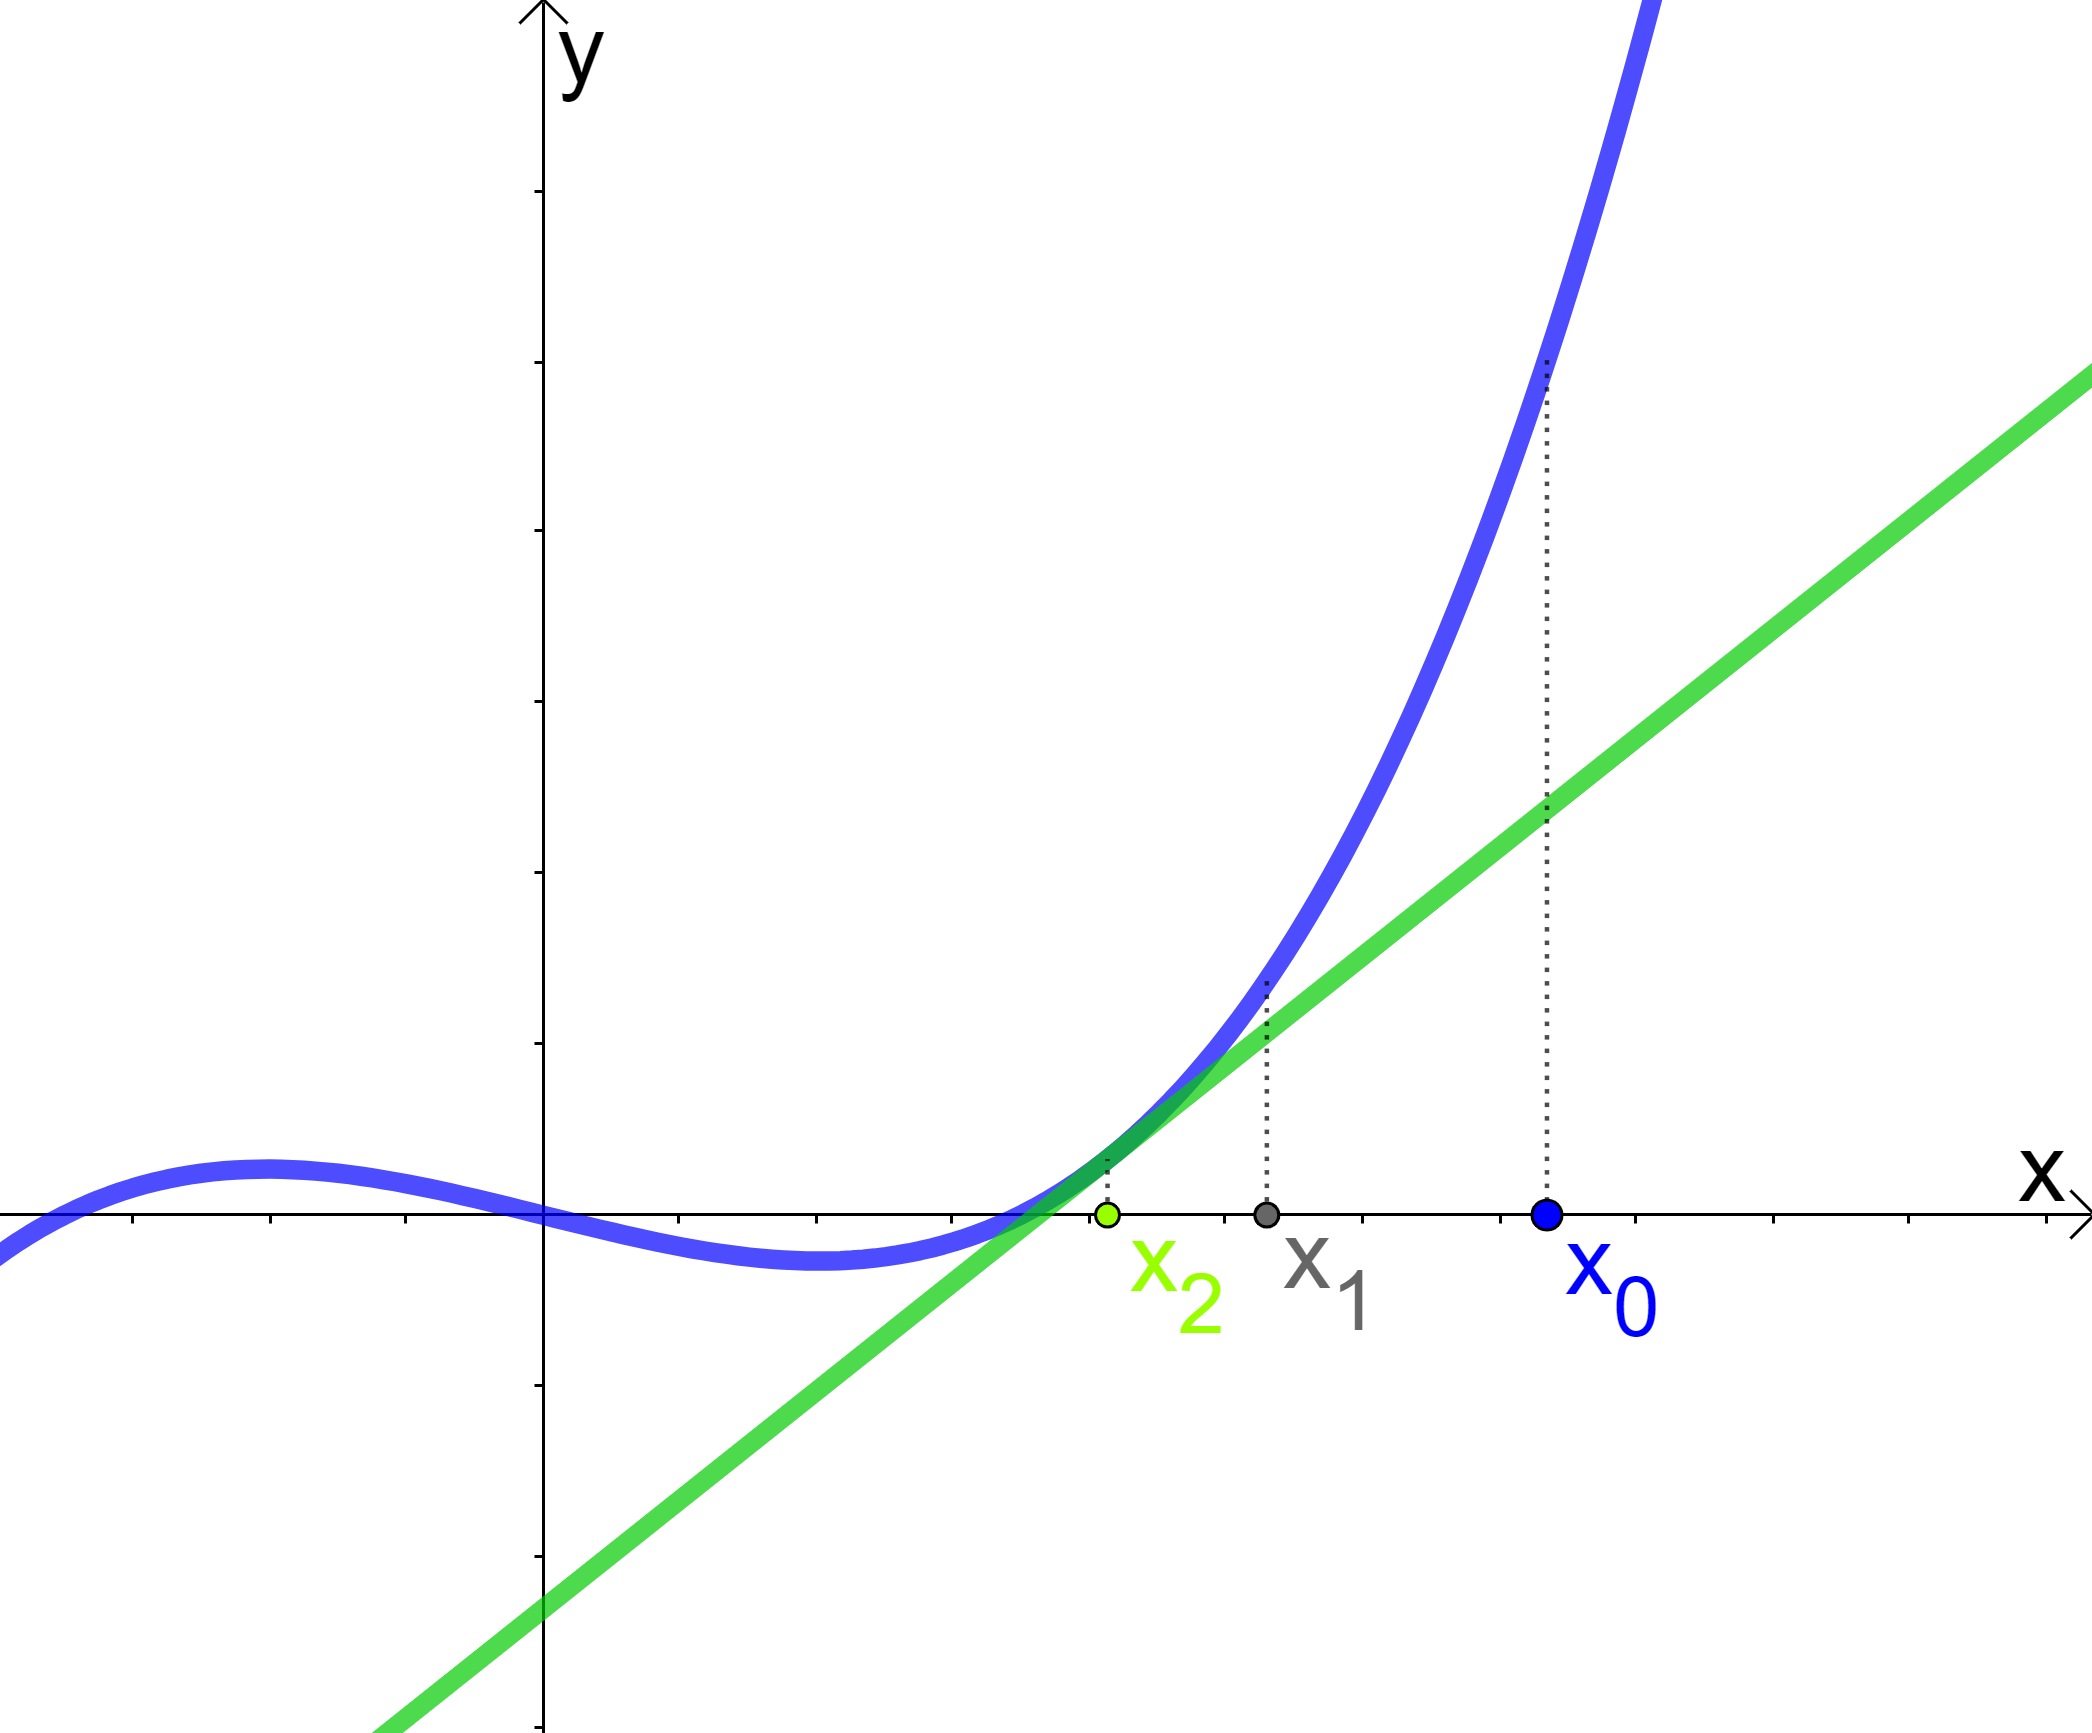
\includegraphics[width=\textwidth]
  {../Mathematik_1/Bilder/newton_tangente_zweite_iteration.png}
\end{minipage}\hfill
\begin{minipage}{0.32\textwidth}
  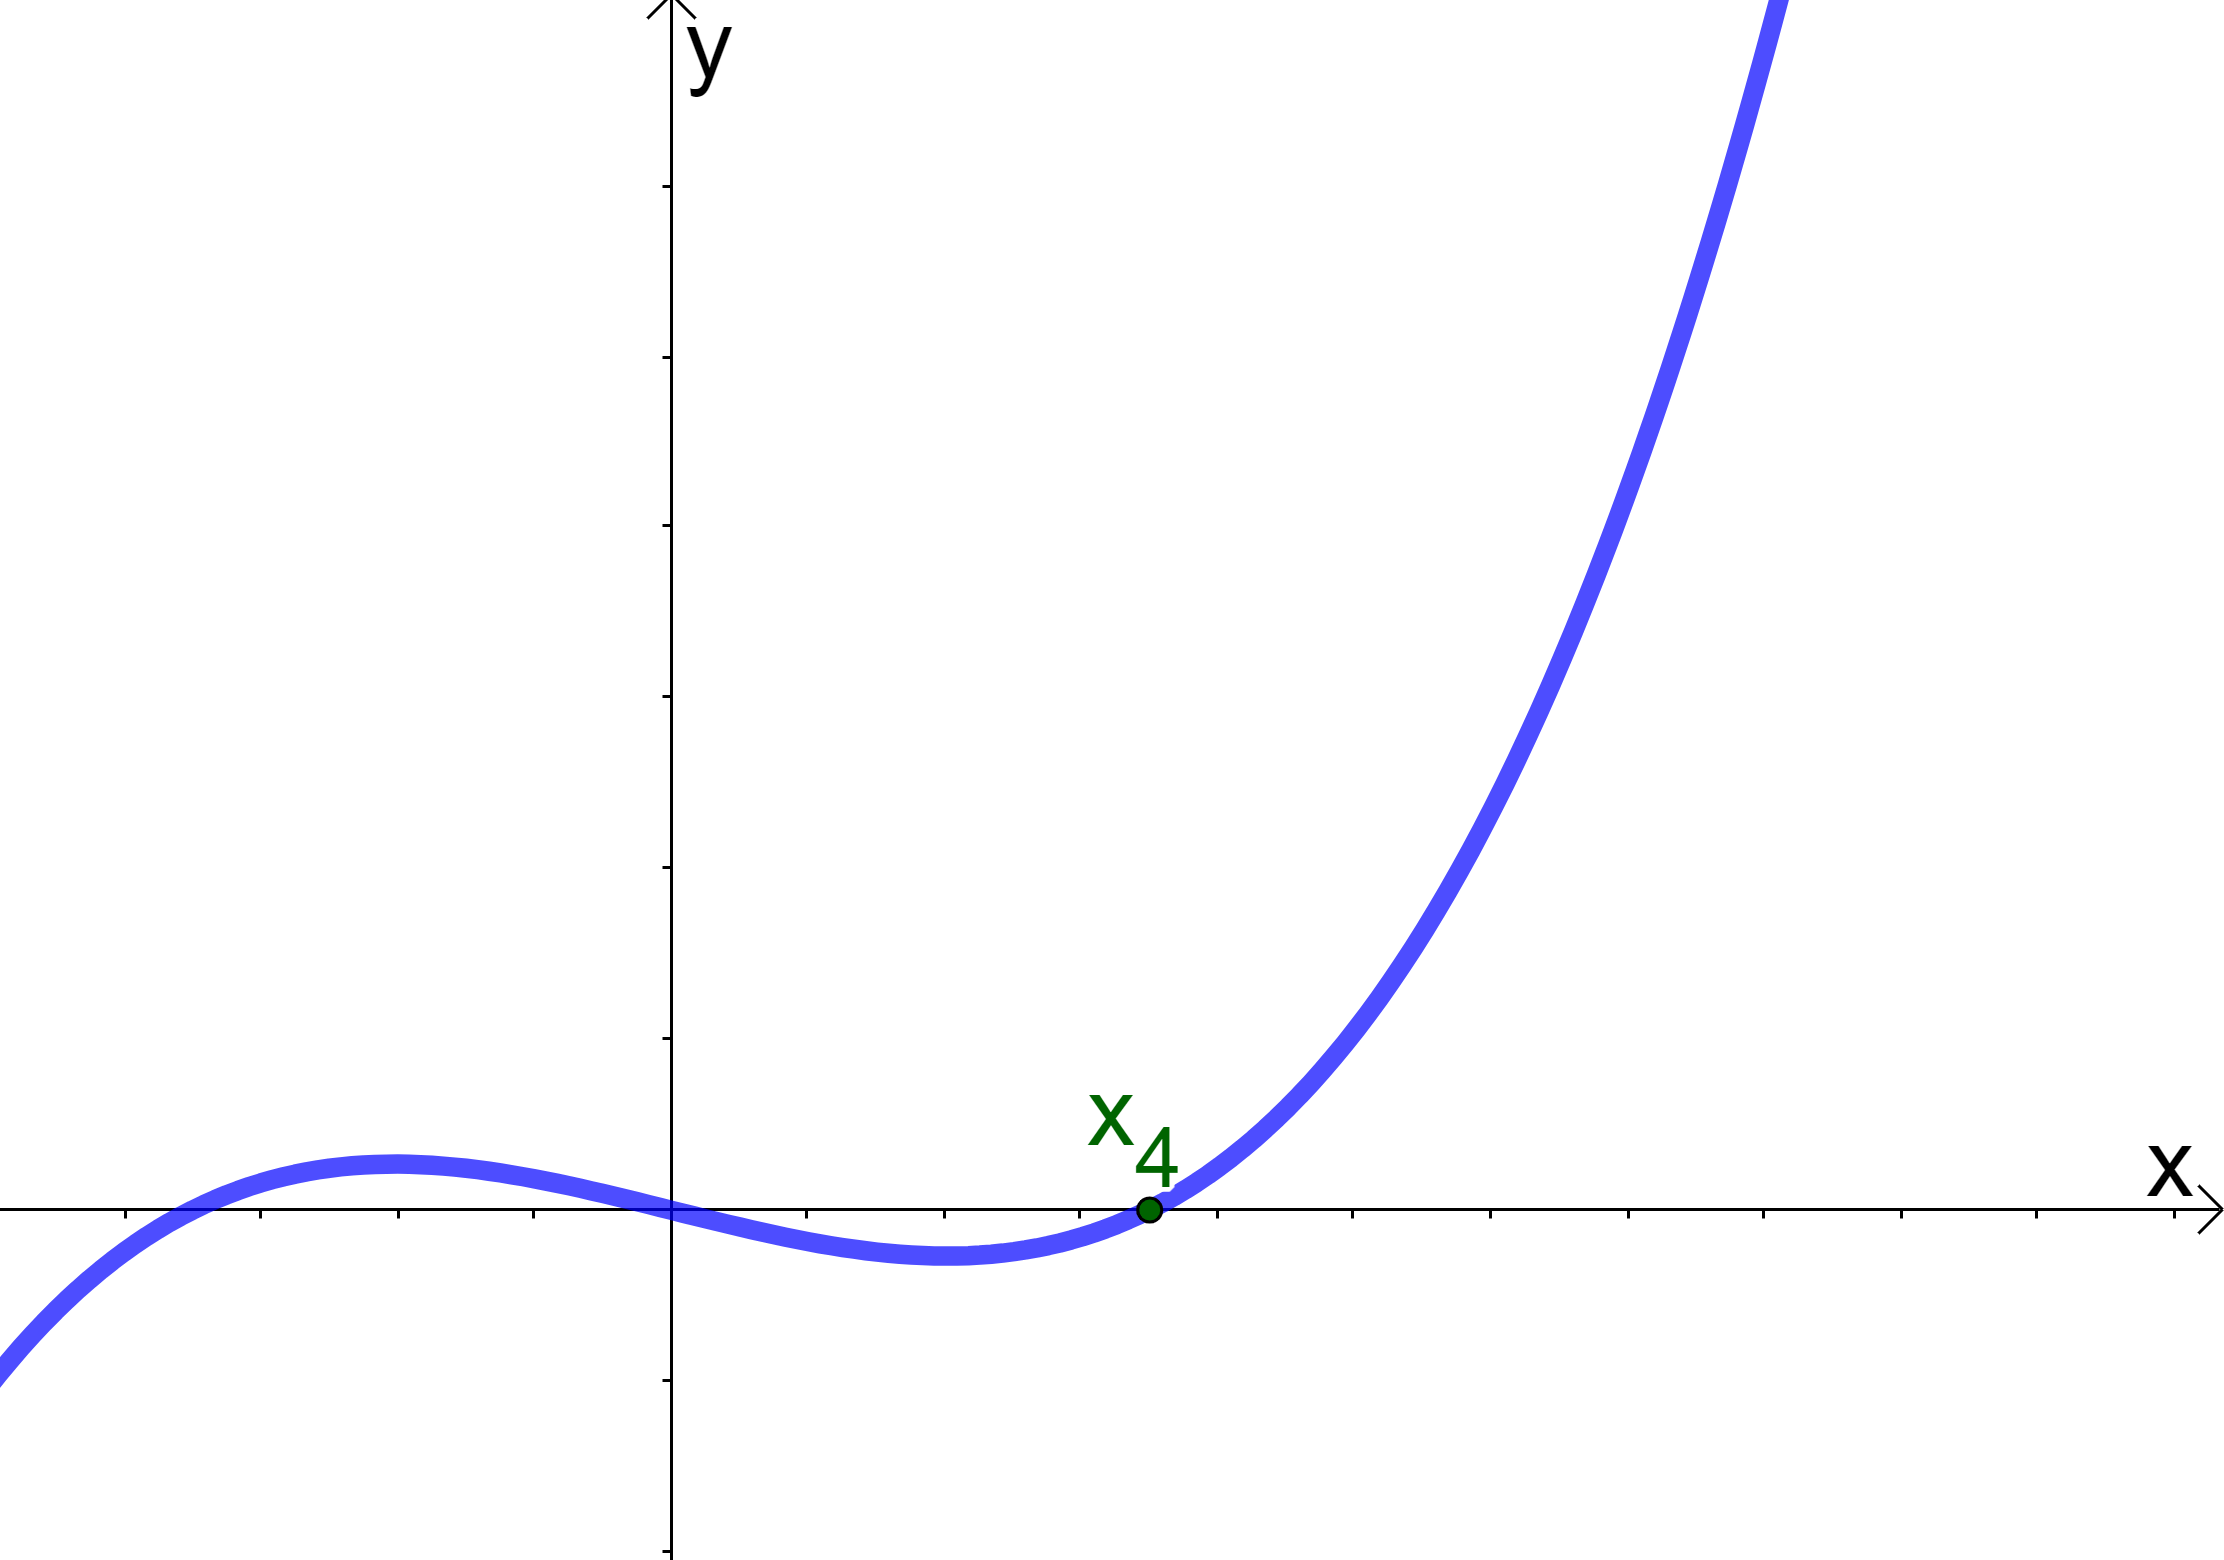
\includegraphics[width=\textwidth]
  {../Mathematik_1/Bilder/newton_naeherung_vierte_iteration.png}
\end{minipage}
\end{exabox}

Die Bildfolge zeigt die wiederholte Linearisierung geometrisch:
An jedem N�herungswert wird die Tangente gebildet. Deren Schnittpunkt mit
der \(x\)-Achse liefert den n�chsten N�herungswert.

Damit zeigt das Newton-Verfahren ein grundlegendes Vorgehen der Numerik:
Ein nichtlineares Problem wird lokal durch ein lineares Problem ersetzt,
das lineare Problem wird gel�st, und anschlie�end wird um die neue
N�herung erneut linearisiert.


\subsubsection*{Abbruch und m�gliche Schwierigkeiten}

In einer numerischen Rechnung kann die Iteration nicht unbegrenzt
fortgesetzt werden. Ein m�gliches Abbruchkriterium ist
\[
|x_{k+1}-x_k|<\varepsilon.
\]
Alternativ kann gepr�ft werden, ob der Funktionswert bereits hinreichend
klein ist:
\[
|f(x_k)|<\varepsilon.
\]

Beide Kriterien messen unterschiedliche Aspekte: Das erste beobachtet,
ob sich die N�herungswerte noch wesentlich ver�ndern, das zweite, wie gut
die aktuelle N�herung die Gleichung \(f(x)=0\) erf�llt.

Das Newton-Verfahren konvergiert nicht f�r jeden Startwert. Besonders
problematisch sind Stellen, an denen
\[
f'(x_k)\approx0.
\]
Die Tangente verl�uft dort nahezu horizontal, sodass der Quotient
\[
\frac{f(x_k)}{f'(x_k)}
\]
sehr gro� werden kann. Der n�chste Newton-Schritt kann dadurch weit vom
gesuchten Bereich wegf�hren.


\begin{exabox}{Schlechter Startwert}{}
\begin{minipage}{0.4\textwidth}
  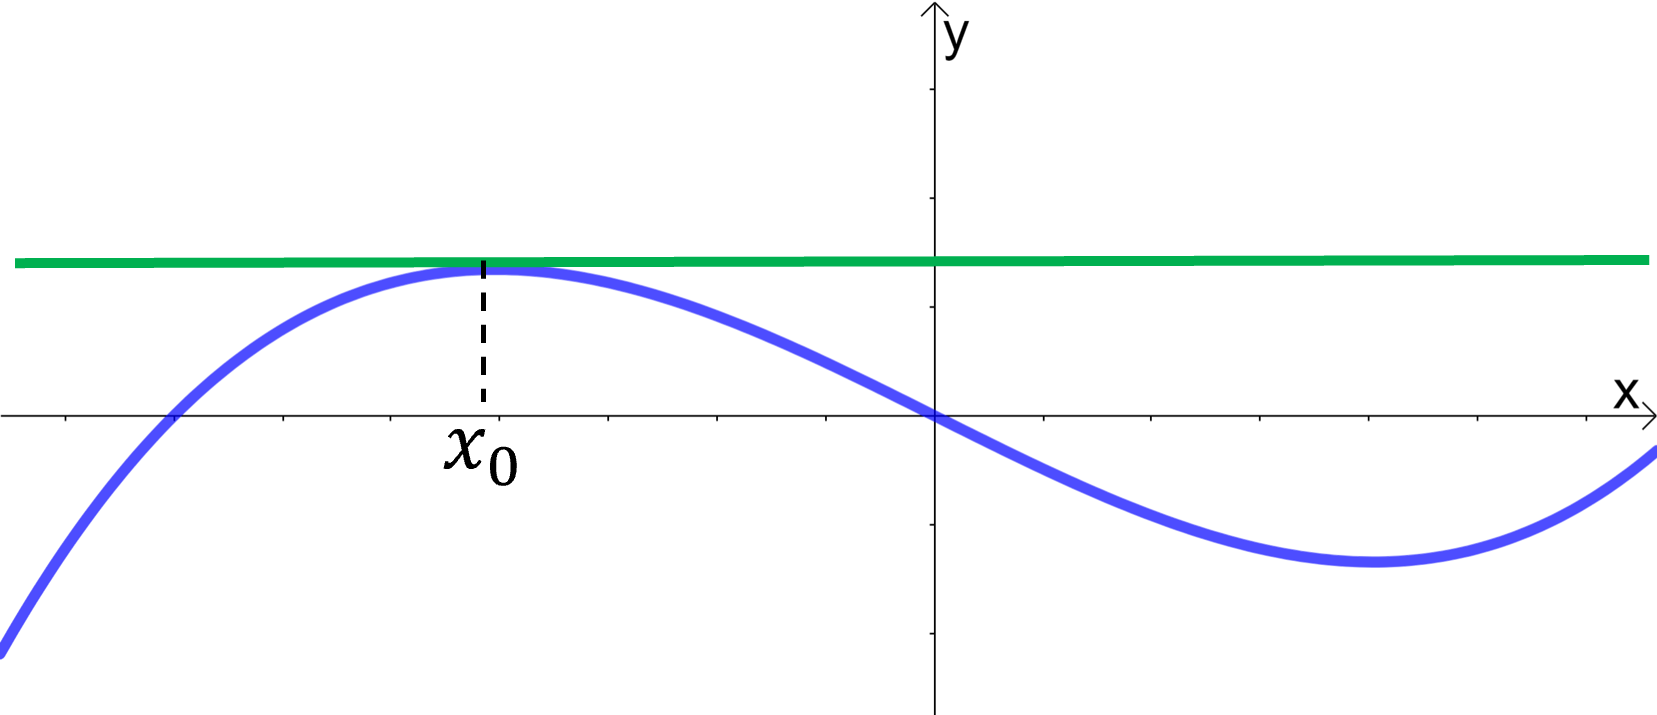
\includegraphics[width=\textwidth]
  {../Mathematik_1/Bilder/newton_problematische_flache_tangente.png}
\end{minipage}\hfill
\begin{minipage}{0.58\textwidth}
Ist die Tangente am aktuellen N�herungswert nahezu horizontal, kann ihr
Schnittpunkt mit der \(x\)-Achse sehr weit entfernt liegen. Die lokale
Linearisierung wird dann au�erhalb des Bereichs verwendet, in dem sie die
Funktion gut approximiert, und der Newton-Schritt kann unbrauchbar werden.
\end{minipage}
\end{exabox}

Gerade dieses m�gliche Scheitern macht noch einmal deutlich, weshalb das
Wort \emph{lokal} entscheidend ist: Eine Tangente beschreibt eine
nichtlineare Funktion nur in der N�he ihres Ber�hrpunktes gut.


% =========================================================
\subsubsection*{Konvergenz des Newton-Verfahrens (+)}

Unter geeigneten Voraussetzungen konvergiert das Newton-Verfahren in der
N�he einer einfachen Nullstelle besonders schnell.

Ist \(x^\ast\) eine Nullstelle mit
\[
f(x^\ast)=0,
\qquad
f'(x^\ast)\neq0,
\]
und ist \(f\) in einer Umgebung von \(x^\ast\) hinreichend glatt, so
konvergiert die Newton-Folge bei einem ausreichend guten Startwert
typischerweise \textbf{quadratisch} gegen \(x^\ast\).

F�r den Fehler
\[
e_k=x_k-x^\ast
\]
bedeutet dies lokal eine Beziehung der Form
\[
|e_{k+1}|
\le
C|e_k|^2.
\]

Ist der Fehler bereits klein, wird er im n�chsten Schritt also ungef�hr
quadriert. Dadurch kann sich die Zahl der korrekten Dezimalstellen in der
N�he der L�sung von einem Schritt zum n�chsten ungef�hr verdoppeln.


\begin{exabox}{Newton-Verfahren f�r \(x^3=7\)}{}

Die Gleichung
\[
x^3=7
\]
wird als Nullstellenproblem
\[
f(x)=x^3-7=0
\]
geschrieben. Wegen
\[
f'(x)=3x^2
\]
lautet die Newton-Iteration
\begin{eqnarray*}
x_{k+1}
&=&
x_k-\frac{x_k^3-7}{3x_k^2}\\[1ex]
&=&
\frac23x_k+\frac{7}{3x_k^2}.
\end{eqnarray*}

Bei einem geeigneten Startwert n�hert sich die Folge sehr schnell der
Nullstelle
\[
x^\ast=\sqrt[3]{7}.
\]
\end{exabox}


% =========================================================

\noindent\textbf{Zusammenfassung:}
Die Beispiele dieses Abschnitts beruhen auf derselben Grundidee.
Differenzierbarkeit erlaubt es, eine nichtlineare Funktion lokal durch
ihre Tangente zu ersetzen. Aus diesem einfachen Gedanken entstehen sehr
unterschiedliche Werkzeuge:

\[
\begin{array}{rcl}
\text{Funktionswert} &\longrightarrow& \text{Tangentenapproximation},\\[0.5ex]
\text{Grenzwert} &\longrightarrow& \text{Vergleich lokaler �nderungsraten},\\[0.5ex]
\text{diskrete Daten} &\longrightarrow& \text{Differenzenquotienten},\\[0.5ex]
\text{nichtlineare Gleichung} &\longrightarrow& \text{Newton-Verfahren}.
\end{array}
\]

Damit ist die Linearisierung nicht nur eine geometrische Interpretation
der Ableitung. Sie ist ein grundlegendes Prinzip, mit dem nichtlineare
Probleme lokal durch einfachere lineare Probleme approximiert werden.
 % Lokale Linearit�t
\newpage
\setcounter{satz}{0} \setcounter{def}{0} \setcounter{exa}{0}  \section{Ableitungen und Funktionsverlauf}\label{MA1-ableitungen-und-funktionsverlauf}

\begin{table}[H]
  \centering
  \begin{tabularx}{\textwidth}{p{0.9\textwidth} p{0.1\textwidth}}
    \toprule
    \multicolumn{2}{c}{\textbf{�bersicht �ber Lernziele und Voraussetzungen}}\\
    \midrule
    \textbf{Lernziele} &\\[.5\normalbaselineskip]
\tabitem das Vorzeichen von \(f^\prime\) als Aussage �ber lokales Steigungsverhalten interpretieren &\\
\tabitem Vorzeichenwechsel von \(f'\) mit lokalen Extrema von \(f\) in Verbindung bringen &\\
\tabitem das Vorzeichen von \(f^{''}\) als Aussage �ber lokales Kr�mmungsverhalten interpretieren &\\
    \tabitem Vorzeichenwechsel von \(f''\) mit Wendestellen in Verbindung bringen &\\
    \midrule
    \textbf{Voraussetzungen} &\\[.5\normalbaselineskip]
    \tabitem Definition der Ableitung & \abschnittsverweis{MA1-stetigkeit-und-differenzierbarkeit}\\
    \tabitem Berechnung von Ableitungen & \abschnittsverweis{MA1-ableitungsregeln}\\
    \tabitem Lokale Linearit�t & \abschnittsverweis{MA1-lokale-linearitaet}\\
    \bottomrule
  \end{tabularx}
\end{table}

\ifintegriereaufgaben
\noindent �bungsaufgaben zum Thema:
\hyperref[MA1-ableitungen-und-funktionsverlauf-aufgaben]{Aufgaben}
\vspace{0.3cm}
\hrule
\fi


% =========================================================
\subsection{Ableitungen beschreiben lokalen Funktionsverlauf}

Die Ableitung einer Funktion ist selbst wieder eine Funktion. W�hrend
\(f\) die betrachtete Gr��e beschreibt, enth�lt \(f'\) Informationen
dar�ber, wie sich diese Gr��e lokal ver�ndert.

Damit er�ffnet die Differentialrechnung zwei unterschiedliche, aber eng
miteinander verbundene Sichtweisen auf eine Funktion.

Die \textbf{Linearisierung} beantwortet die Frage, durch welche einfache
Funktion \(f\) in unmittelbarer Umgebung eines Punktes approximiert
werden kann. Die Ableitungsfunktionen \(f'\), \(f''\), \ldots{} erlauben
dagegen qualitative Aussagen dar�ber, wie sich der Funktionsverlauf lokal
verh�lt.

Die erste Ableitung beschreibt die lokale �nderung von \(f\):
\[
f'(x)>0
\quad\Longrightarrow\quad
f\text{ w�chst lokal},
\]
w�hrend
\[
f'(x)<0
\quad\Longrightarrow\quad
f\text{ f�llt lokal}.
\]

Die zweite Ableitung beschreibt, wie sich diese lokale �nderungsrate
selbst ver�ndert. Sie gibt damit Auskunft dar�ber, ob die Steigung
zunimmt oder abnimmt und wie sich der Graph kr�mmt.

Ableitungen liefern somit nicht nur Zahlen. Ihre Vorzeichen und
Vorzeichenwechsel enthalten qualitative Informationen �ber den Verlauf
der urspr�nglichen Funktion.


% =========================================================
\subsection{Die erste Ableitung: Wachstum und Abnahme}

Ist \(f'(x_0)>0\), so besitzt die Tangente an \(f\) in \(x_0\) eine
positive Steigung. In hinreichend kleiner Umgebung von \(x_0\) nimmt
die Funktion daher zu.

Entsprechend bedeutet \(f'(x_0)<0\), dass die Tangente eine negative
Steigung besitzt und die Funktion lokal abnimmt.

Aus einer punktweisen Aussage wird eine Aussage �ber einen ganzen
Funktionsabschnitt, wenn das Vorzeichen der Ableitung auf einem Intervall
bekannt ist.

\begin{theorembox}{Vorzeichen von \(f'\) und Monotonie}{}
Es sei \(f\) auf einem Intervall \(I\) differenzierbar.

Gilt
\[
f'(x)>0
\qquad\text{f�r alle }x\in I,
\]
so ist \(f\) auf \(I\) streng monoton wachsend.

Gilt
\[
f'(x)<0
\qquad\text{f�r alle }x\in I,
\]
so ist \(f\) auf \(I\) streng monoton fallend.
\end{theorembox}

Die Ableitungsfunktion liefert damit eine qualitative Beschreibung des
Funktionsverlaufs, ohne dass alle Funktionswerte von \(f\) einzeln
betrachtet werden m�ssen.

Besonders interessant sind Stellen, an denen sich das Vorzeichen von
\(f'\) �ndert.

Wechselt \(f'\) von positiv nach negativ, so geht die Funktion lokal von
Wachstum zu Abnahme �ber:
\[
f':\quad +\longrightarrow-
\qquad\Longrightarrow\qquad
\text{lokales Maximum}.
\]

Wechselt \(f'\) von negativ nach positiv, so geht die Funktion lokal von
Abnahme zu Wachstum �ber:
\[
f':\quad -\longrightarrow+
\qquad\Longrightarrow\qquad
\text{lokales Minimum}.
\]

An einer solchen Extremstelle besitzt eine differenzierbare Funktion eine
horizontale Tangente. F�r einen inneren Punkt \(x_0\) gilt daher
notwendigerweise
\[
f'(x_0)=0.
\]

Die Umkehrung gilt jedoch nicht: Eine horizontale Tangente allein bedeutet
noch nicht, dass dort ein Extremum vorliegt.


\begin{exabox}{Der Vorzeichenwechsel entscheidet}{}

\begin{minipage}{0.58\textwidth}
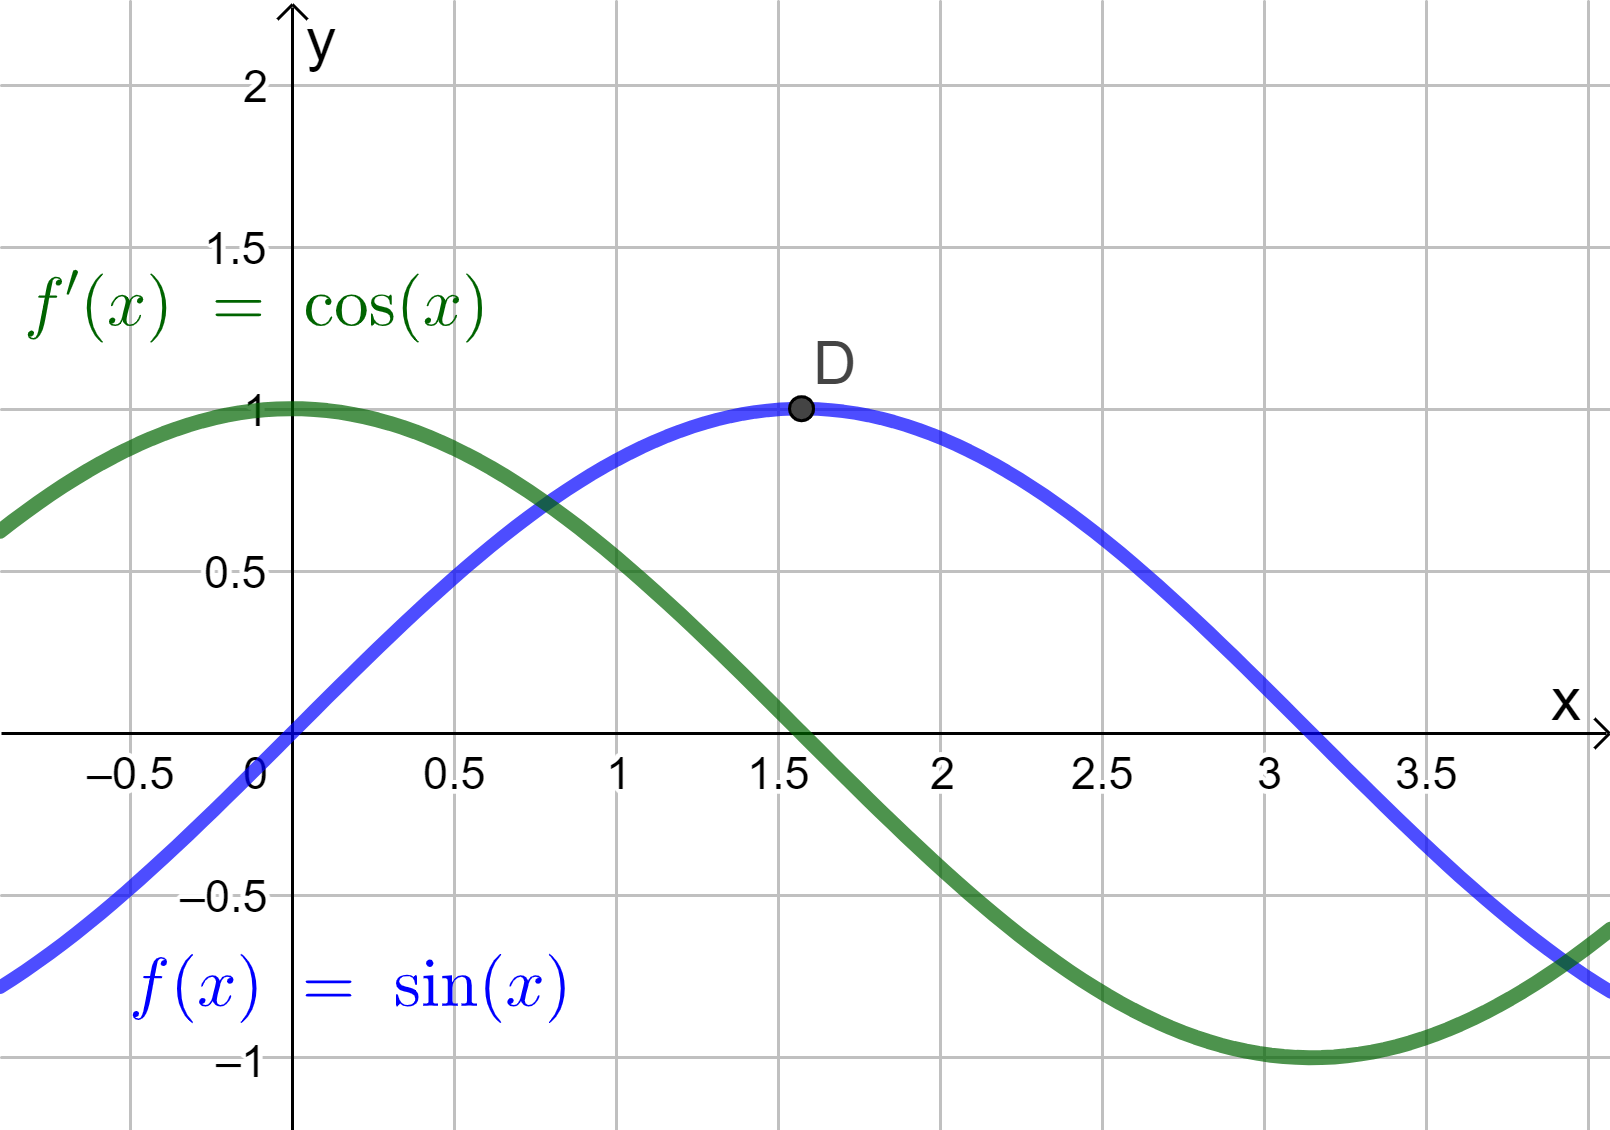
\includegraphics[width=\textwidth]
{../Mathematik_1/Bilder/ableitung_sinus_kosinus.png}
\end{minipage}
\hfill
\begin{minipage}{0.40\textwidth}

F�r
\[
f(x)=\sin(x)
\]
gilt
\[
f'(x)=\cos(x).
\]

Bei \(x_0=\pi/2\) verschwindet die Ableitung und wechselt ihr Vorzeichen:
\[
+\longrightarrow-.
\]

Die Sinusfunktion geht dort von Wachstum zu Abnahme �ber. Sie besitzt
folglich ein lokales Maximum.
\end{minipage}

\vspace{2ex}

\begin{minipage}{0.58\textwidth}
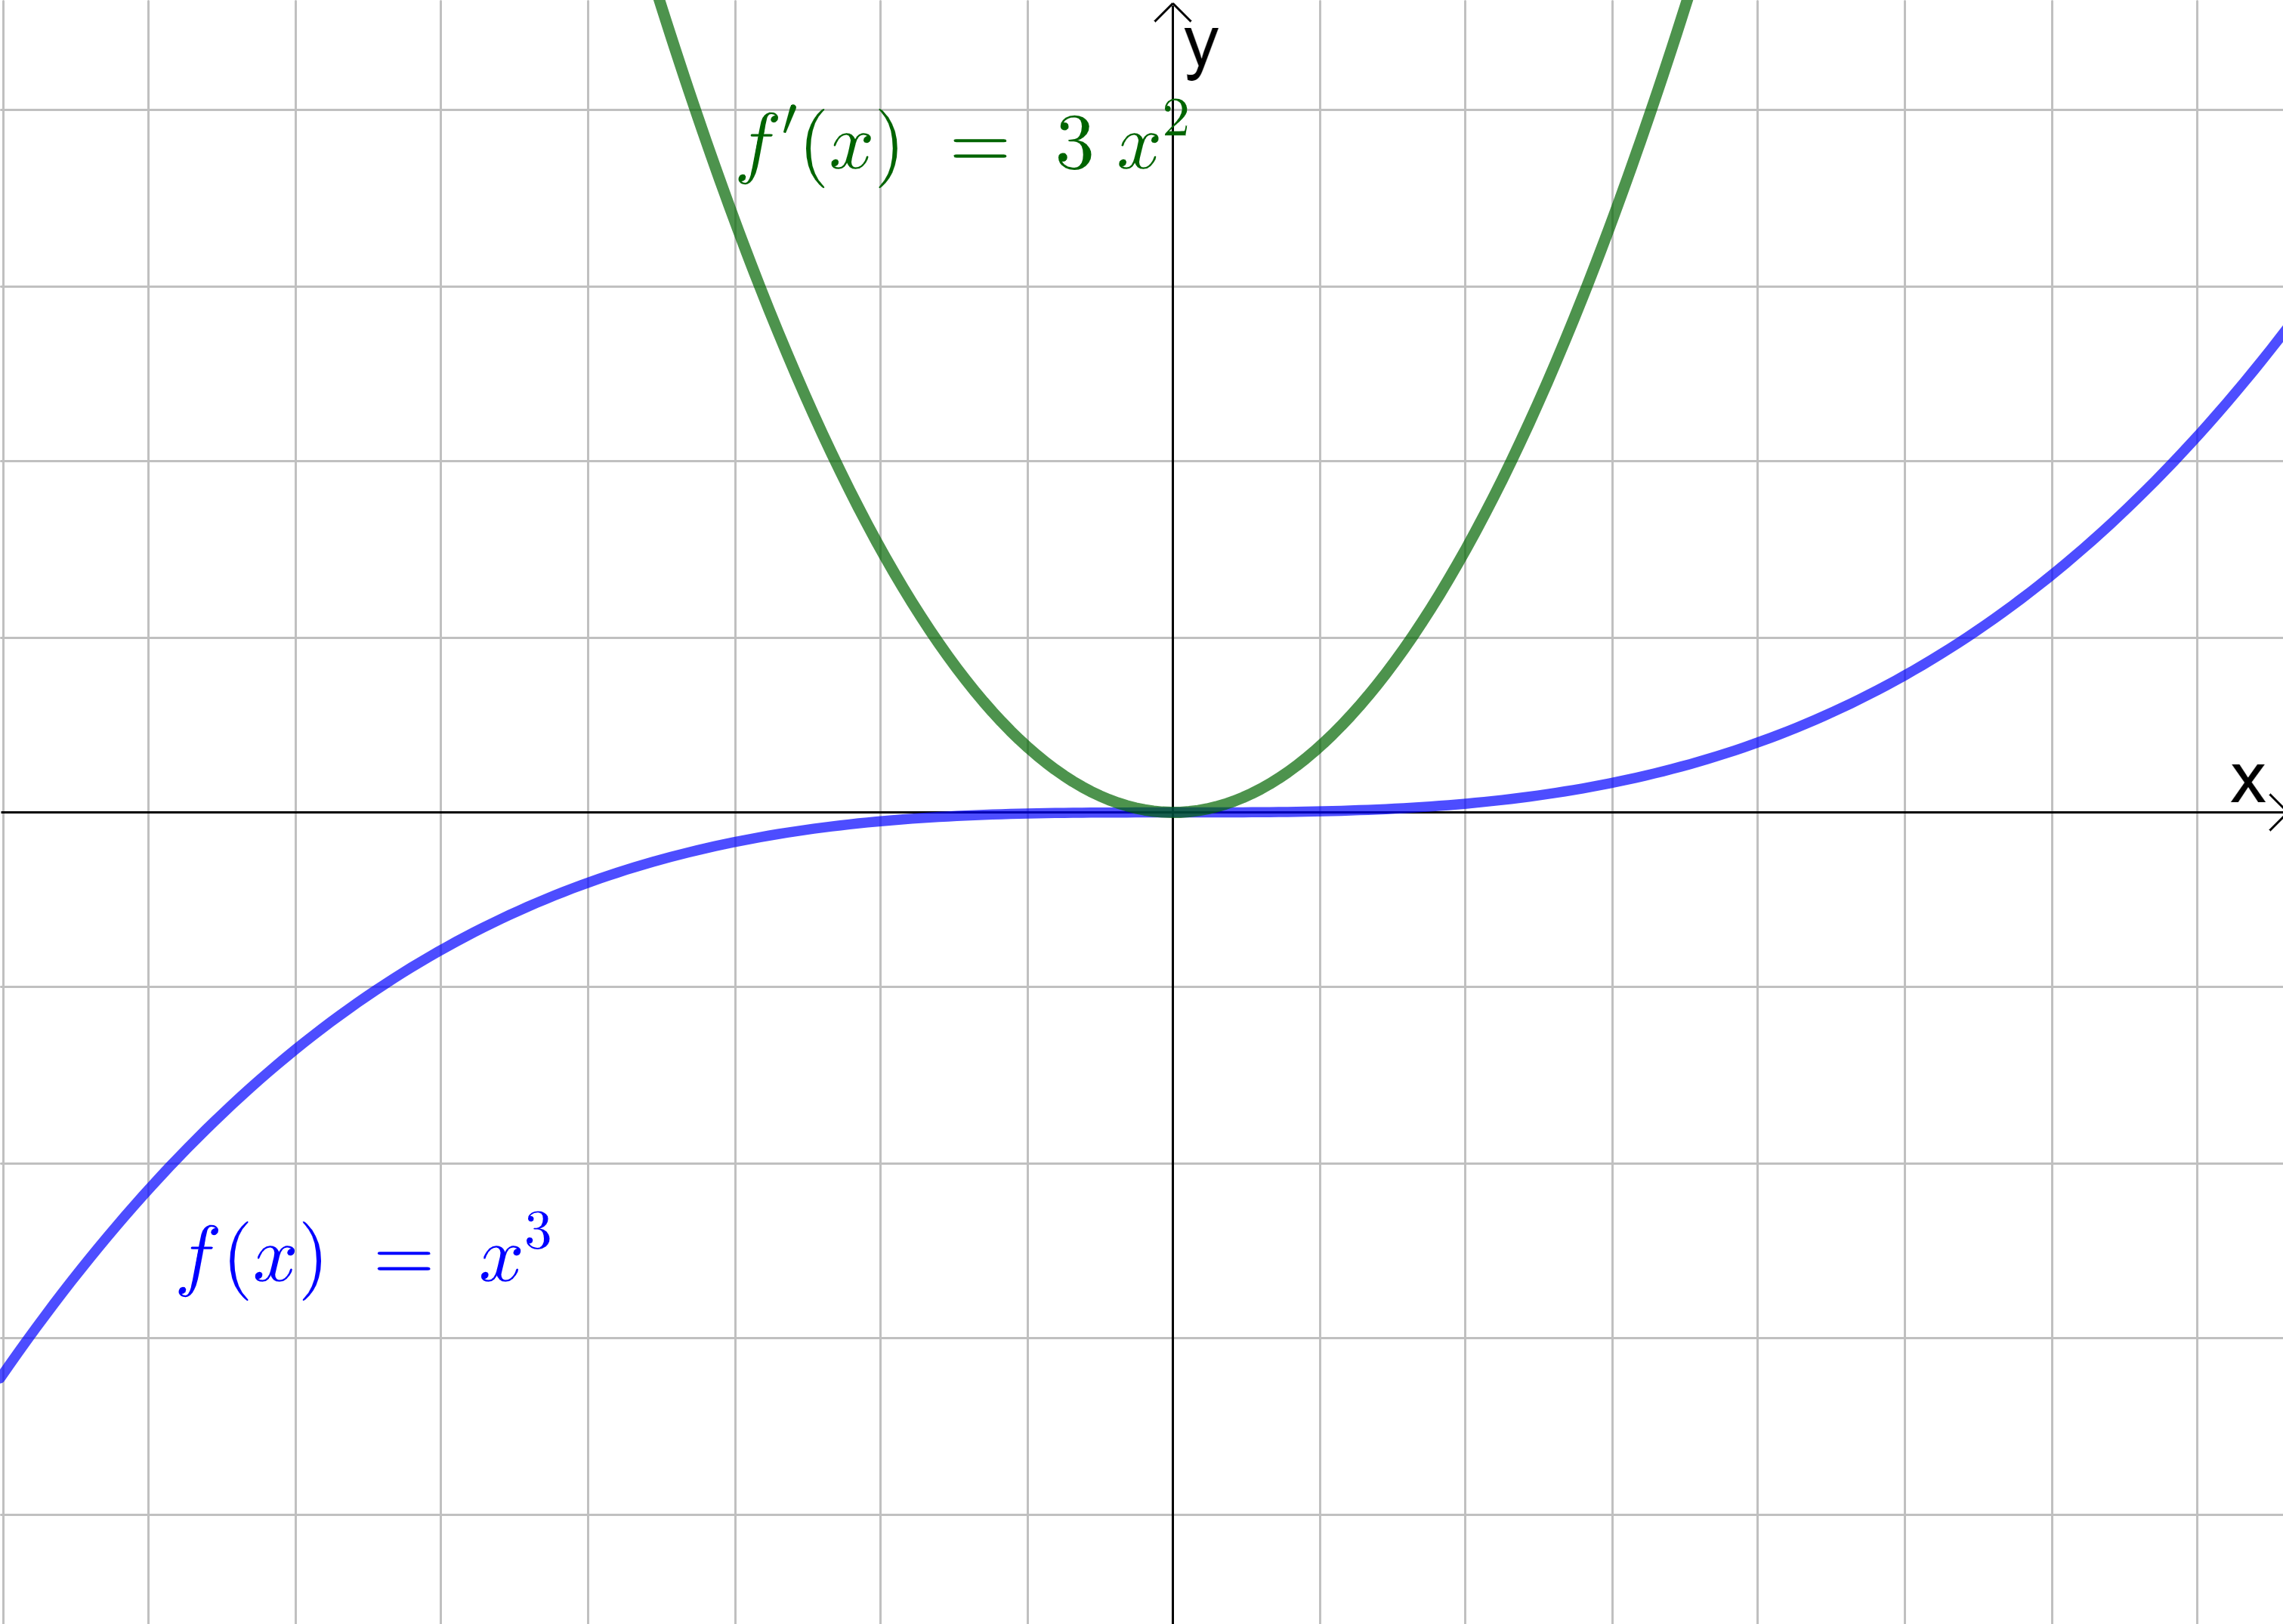
\includegraphics[width=\textwidth]
{../Mathematik_1/Bilder/extremstellen_potenz_drei_gegenbeispiel.png}
\end{minipage}
\hfill
\begin{minipage}{0.40\textwidth}

F�r
\[
f(x)=x^3
\]
gilt
\[
f'(x)=3x^2.
\]

Auch hier ist
\[
f'(0)=0.
\]
Die Ableitung bleibt jedoch auf beiden Seiten von \(0\) positiv. Die
Funktion w�chst also vor und nach \(x_0=0\).

Es liegt kein lokales Extremum vor.
\end{minipage}

\end{exabox}

Das Beispiel zeigt einen wichtigen Unterschied: Die Gleichung
\[
f'(x_0)=0
\]
liefert zun�chst nur eine Stelle mit horizontaler Tangente. Erst das
lokale Verhalten von \(f'\) um \(x_0\) zeigt, was dort mit der Funktion
geschieht.


% =========================================================
\subsection{Die zweite Ableitung: Wie ver�ndert sich die Steigung?}

Die erste Ableitung \(f'\) beschreibt die Steigung von \(f\). Die zweite
Ableitung
\[
f''=(f')'
\]
beschreibt daher, wie sich diese Steigung ver�ndert.

Ist
\[
f''(x)>0,
\]
so nimmt \(f'(x)\) lokal zu. Die Steigungen von \(f\) werden also gr��er.

Ist dagegen
\[
f''(x)<0,
\]
so nimmt \(f'(x)\) lokal ab. Die Steigungen von \(f\) werden kleiner.

Diese Aussage ist zun�chst unabh�ngig davon, ob \(f\) selbst gerade
steigt oder f�llt. Beispielsweise kann eine Funktion fallen und dabei
immer flacher werden. In diesem Fall ist
\[
f'(x)<0,
\qquad
f''(x)>0.
\]

Die Vorzeichen von \(f'\) und \(f''\) beschreiben also unterschiedliche
Eigenschaften:

\[
\begin{array}{ccl}
f'(x) &:& \text{Richtung der lokalen �nderung von }f,\\[0.5ex]
f''(x)&:& \text{�nderung dieser lokalen Steigung}.
\end{array}
\]

Geometrisch f�hrt die zweite Ableitung zur
\textbf{Kr�mmung} (\emph{curvature behaviour}) des Graphen.

\begin{theorembox}{Vorzeichen von \(f''\) und Kr�mmung}{}
Es sei \(f\) auf einem Intervall \(I\) zweimal differenzierbar.

Gilt
\[
f''(x)>0
\qquad\text{f�r alle }x\in I,
\]
so ist \(f\) auf \(I\) konvex.

Gilt
\[
f''(x)<0
\qquad\text{f�r alle }x\in I,
\]
so ist \(f\) auf \(I\) konkav.
\end{theorembox}

Eine �nderung des Vorzeichens von \(f''\) zeigt einen Wechsel des
Kr�mmungsverhaltens an. Eine solche Stelle hei�t
\textbf{Wendestelle} (\emph{inflection point} f�r den zugeh�rigen Punkt
des Graphen).

F�r eine hinreichend glatte Funktion gilt an einer inneren Wendestelle
notwendigerweise
\[
f''(x_0)=0.
\]

Wie schon bei der ersten Ableitung reicht das Verschwinden der Ableitung
allein jedoch nicht aus. Entscheidend ist wiederum das lokale Verhalten:
Das Vorzeichen von \(f''\) muss sich �ndern.


\begin{exabox}{Wendestelle als �nderung des lokalen Verhaltens}{}

\begin{minipage}{0.58\textwidth}
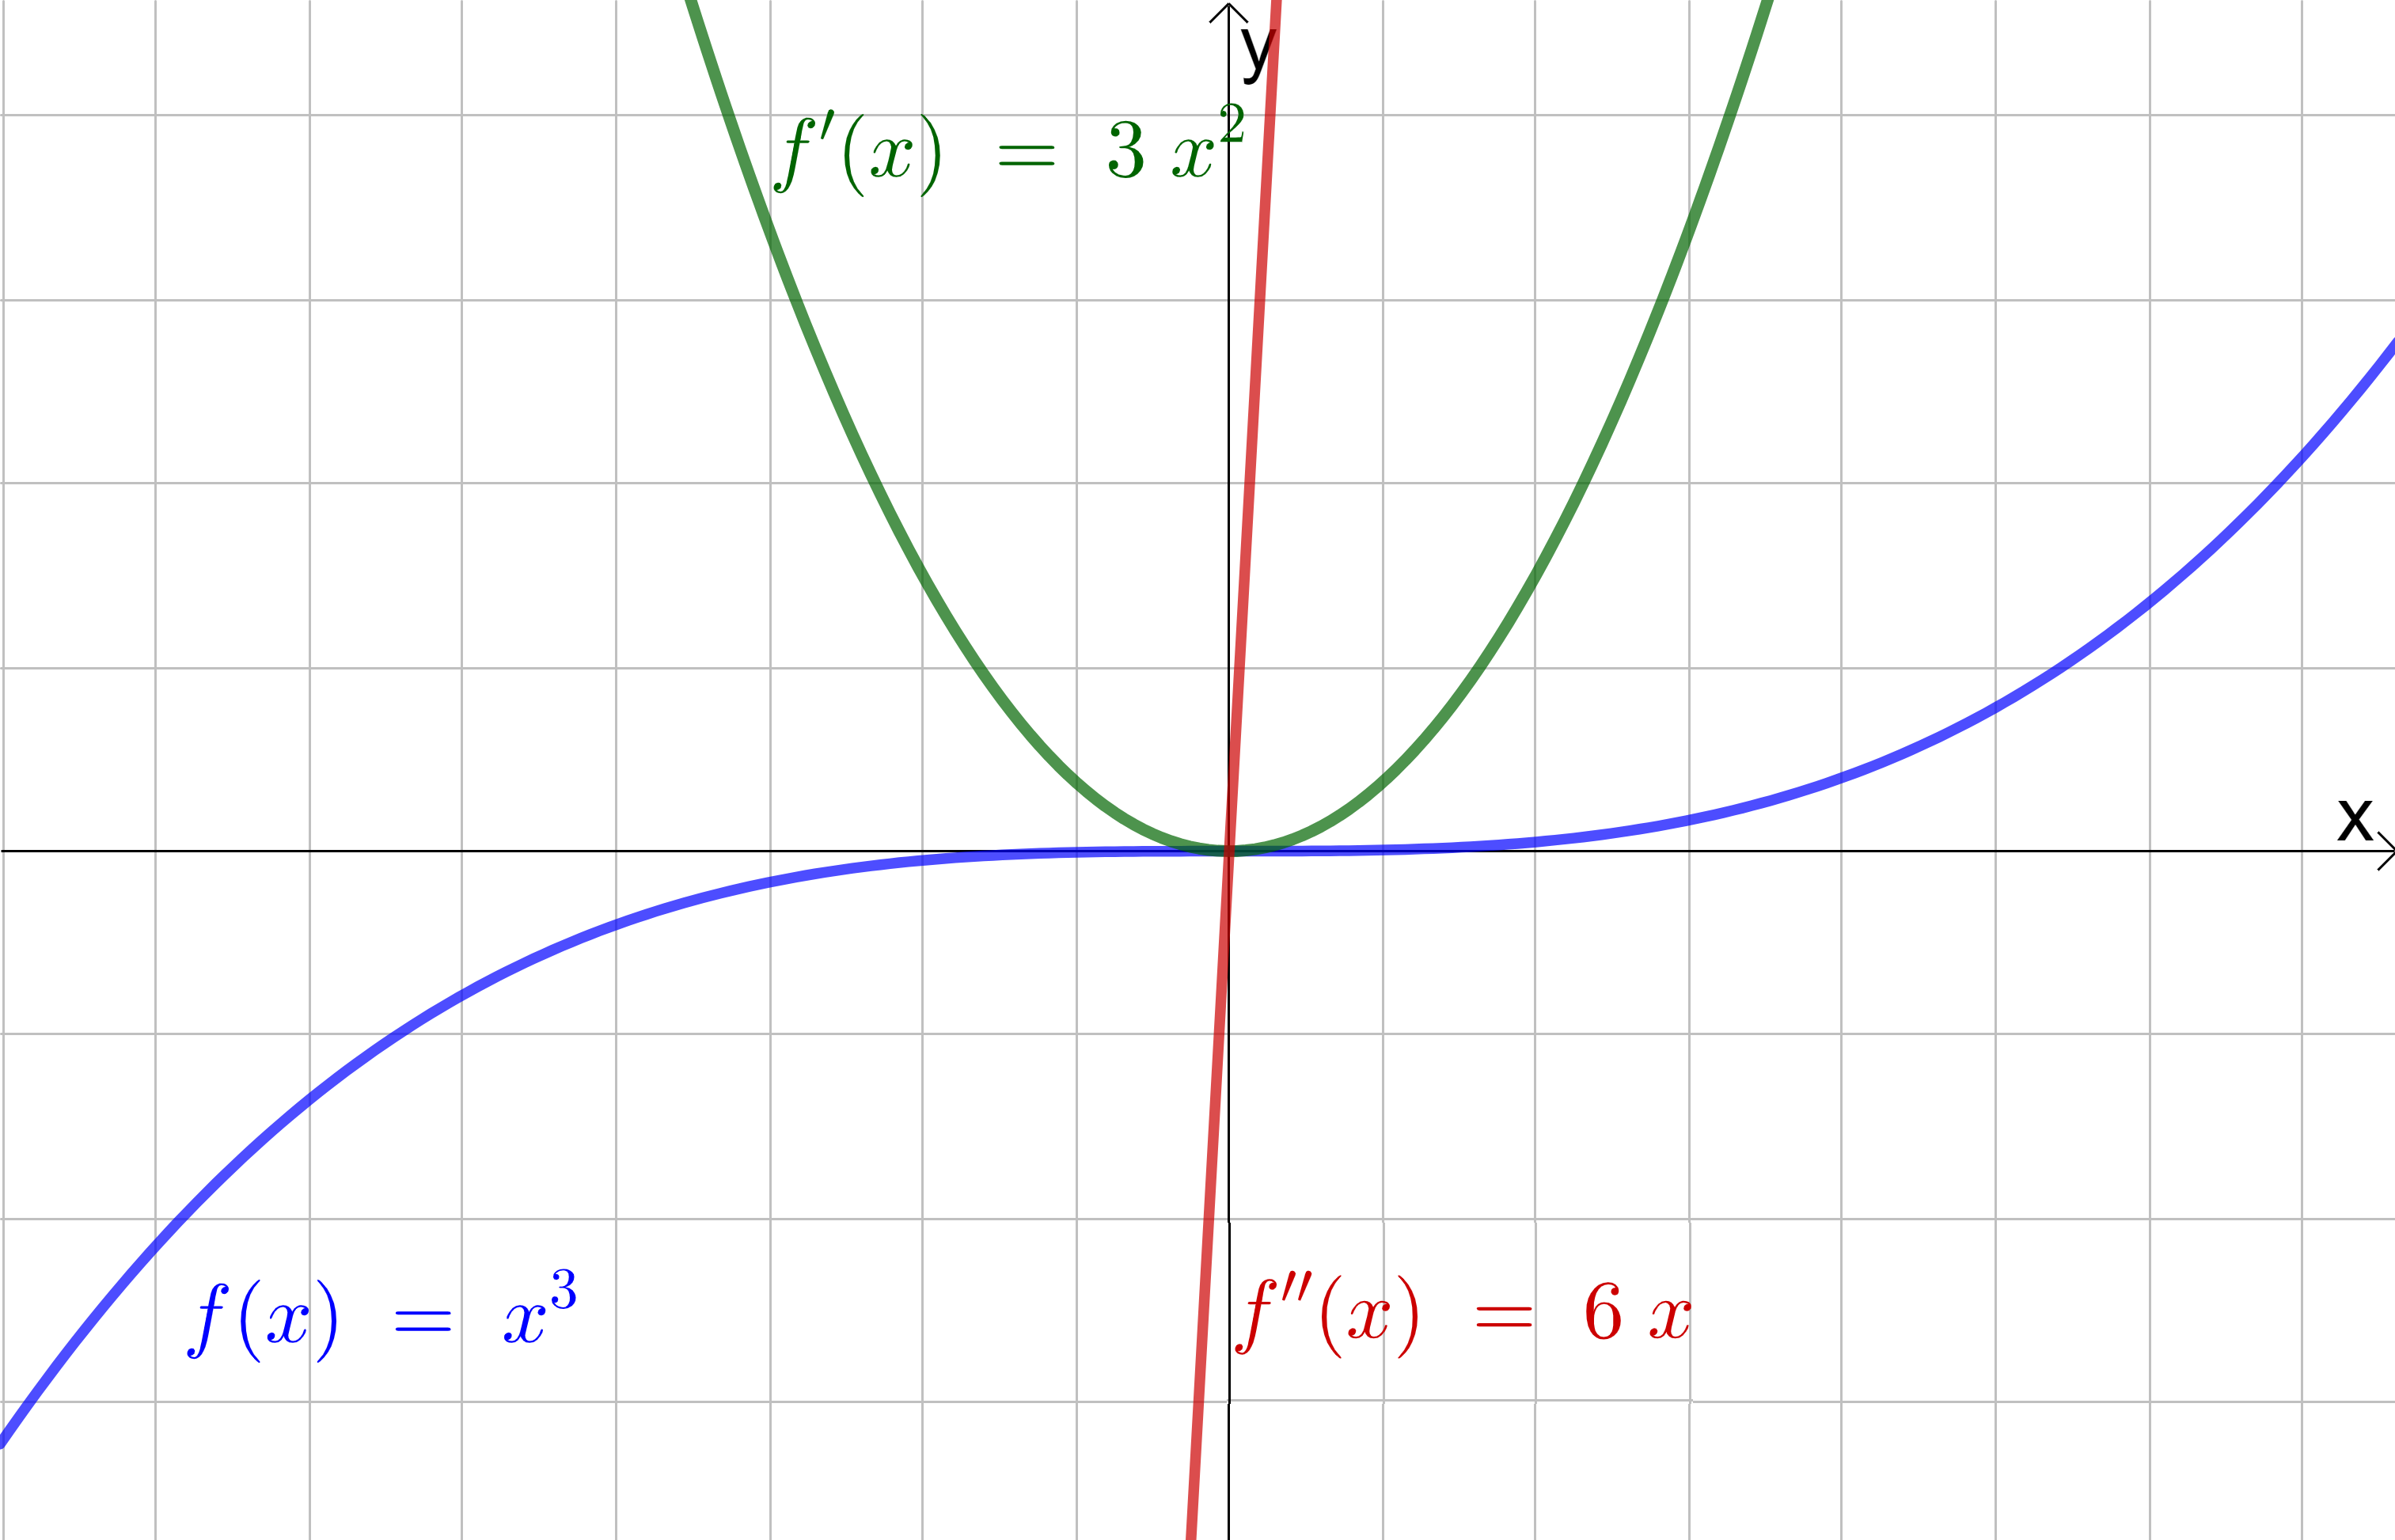
\includegraphics[width=\textwidth]
{../Mathematik_1/Bilder/wendestellen_potenz_drei_ableitungen.png}
\end{minipage}
\hfill
\begin{minipage}{0.40\textwidth}

F�r
\[
f(x)=x^3
\]
gilt
\[
f''(x)=6x.
\]

Damit ist
\[
f''(x)<0
\quad\text{f�r }x<0,
\]
und
\[
f''(x)>0
\quad\text{f�r }x>0.
\]

Die zweite Ableitung wechselt bei \(x_0=0\) ihr Vorzeichen. Dort �ndert
sich das Kr�mmungsverhalten der Funktion: \(x_0=0\) ist eine Wendestelle.
\end{minipage}

\end{exabox}


% =========================================================
\subsection{Ableitungen als qualitative Information}

Die ersten beiden Ableitungen lassen sich gemeinsam lesen. Dabei geht es
nicht in erster Linie darum, einzelne ausgezeichnete Punkte zu berechnen.
Vielmehr beschreiben \(f'\) und \(f''\), wie sich eine Funktion lokal
verh�lt.

F�r einen Punkt \(x\) liefern bereits die Vorzeichen
\[
f'(x)
\qquad\text{und}\qquad
f''(x)
\]
eine qualitative Charakterisierung.

\begin{center}
\begin{tabular}{c|c|c}
 & \(f''(x)>0\) & \(f''(x)<0\)\\
\hline
\(f'(x)>0\)
&
wachsend, Steigung nimmt zu
&
wachsend, Steigung nimmt ab
\\[0.5ex]
\(f'(x)<0\)
&
fallend, Steigung nimmt zu
&
fallend, Steigung nimmt ab
\end{tabular}
\end{center}

So bedeutet beispielsweise
\[
f'(x)>0,
\qquad
f''(x)<0,
\]
dass die Funktion zwar w�chst, ihre Steigung aber abnimmt: Der Graph
steigt weiter, wird dabei jedoch zunehmend flacher.

Dagegen bedeutet
\[
f'(x)<0,
\qquad
f''(x)>0,
\]
dass die Funktion f�llt, ihre Steigung aber zunimmt. Die Steigung ist
noch negativ, n�hert sich jedoch m�glicherweise der horizontalen
Richtung an.

Diese Aussagen sind lokal. Sie beschreiben das Verhalten einer Funktion
in der Umgebung eines Punktes oder auf einem Intervall, auf dem die
entsprechenden Vorzeichen erhalten bleiben.


% =========================================================
\subsection{Vom lokalen Verhalten zum Gesamtbild}

Werden die lokalen Informationen f�r verschiedene Bereiche des
Definitionsgebiets zusammengesetzt, entsteht schrittweise ein
qualitatives Bild des gesamten Funktionsverlaufs.

Nullstellen von \(f'\) markieren dabei Stellen, an denen sich das
Monotonieverhalten �ndern kann. Nullstellen von \(f''\) markieren Stellen,
an denen sich das Kr�mmungsverhalten �ndern kann. Entscheidend ist jeweils
nicht allein die Nullstelle der Ableitung, sondern das Verhalten der
Ableitungsfunktion auf beiden Seiten.

Die klassische \textbf{Kurvendiskussion} fasst solche Informationen
systematisch zusammen. F�r die hier betrachtete lokale Sichtweise steht
jedoch nicht das vollst�ndige Berechnungsschema im Vordergrund, sondern
die �bersetzung
\[
\text{Eigenschaften von }f',f''
\quad\longrightarrow\quad
\text{qualitative Eigenschaften von }f.
\]


%\begin{exabox}{Aus lokalen Informationen entsteht ein Funktionsverlauf}{}
%\begin{center}
%\includegraphics[width=0.45\textwidth]
%{../Mathematik_1/Bilder/28_Kurvendiskussion.png}
%\end{center}
%\end{exabox}


% =========================================================
\subsection*{Zwei lokale Sichtweisen auf eine Funktion}

Die Differentialrechnung dieses Kapitels hat damit zwei eng verbundene
M�glichkeiten hervorgebracht, das lokale Verhalten einer Funktion zu
untersuchen.

Bei der \textbf{Linearisierung} wird die Funktion selbst in der Umgebung
eines Punktes durch ihre Tangente approximiert:
\[
f(x_0+h)
=
f(x_0)+f'(x_0)h+o(h).
\]
Die Ableitung liefert dabei das lokale lineare Modell.

Die \textbf{Interpretation der Ableitungsfunktionen} verfolgt eine andere
Frage. Aus dem Vorzeichen und dem Verlauf von \(f'\) und \(f''\) werden
qualitative Aussagen �ber die urspr�ngliche Funktion gewonnen:
\[
\begin{array}{rcl}
f' &\longrightarrow& \text{Wachstum und Abnahme},\\[0.5ex]
f''&\longrightarrow& \text{Ver�nderung der Steigung und Kr�mmung}.
\end{array}
\]

Beide Sichtweisen sind lokal. Die eine approximiert die Funktion in der
N�he eines Punktes, die andere charakterisiert dort ihren Verlauf.

Damit liefert die Ableitung sowohl ein lokales Ersatzmodell als auch
Informationen dar�ber, wie sich eine Funktion ver�ndert.

 % Ableitungen und Funktionsverlauf



% Mathematik 2 % ohne �bungsbl�ttern und L�sungen
\part{Mathematik 2 -- Systeme und globale Dynamik}

\chapter*{Leitidee}
\addcontentsline{toc}{chapter}{Leitidee}

\textbf{Leitidee}

In \textbf{Mathematik 1} standen lokale Eigenschaften von Funktionen im Mittelpunkt.
Ableitungen beschreiben das Verhalten einer Funktion in der unmittelbaren Umgebung
eines Punktes. Damit lassen sich Tangenten, Extremstellen und Wendepunkte bestimmen
und lokale Dynamik analysieren.

Dar�ber hinaus haben wir grundlegende Bausteine kennengelernt:
Exponentialfunktionen modellieren Wachstum und Zerfall, und komplexe Zahlen
erm�glichen es, Drehungen und Schwingungen algebraisch zu beschreiben.
Mit der Eulerschen Identit�t
\[
e^{ix}=\cos(x)+i\sin(x)
\]
wird sichtbar, dass Exponentialfunktionen und harmonische Schwingungen
eng miteinander verbunden sind.

In \textbf{Mathematik 2} erweitern wir diese Perspektive.
Funktionen werden nicht mehr nur punktweise untersucht,
sondern als Elemente strukturierter R�ume betrachtet.
Damit wird es m�glich, Funktionen und Signale global zu beschreiben,
zu rekonstruieren und in einfachere Bausteine zu zerlegen.

Die zentralen Werkzeuge daf�r sind
\emph{Integration}, \emph{Projektionen in Funktionenr�umen} (Bestapproximation)
sowie die \emph{Fourieranalyse}.
Mit Hilfe geeigneter Transformationen lassen sich au�erdem dynamische Prozesse
und technische Systeme systematisch analysieren.

Der konzeptionelle �bergang l�sst sich so zusammenfassen:

\medskip

\begin{center}
\textbf{Lokal:} Tangente / Schmiegeparabel $\Rightarrow$ Taylor-Polynome \qquad
\textbf{Global:} Projektion / Transformation $\Rightarrow$ Fourier \& Laplace
\end{center}

Mathematik 2 zeigt damit, dass Funktionen nicht nur Rechenvorschriften sind,
sondern Elemente strukturierter R�ume, deren Eigenschaften durch Projektion,
Zerlegung und Transformation sichtbar werden.
Diese Sichtweise bildet die Grundlage f�r das mathematische Verst�ndnis
technischer Systeme.
 \newpage % Idee

\chapter{Von lokaler zu globaler N�herung}

\section*{Leitidee}
Dieses Kapitel markiert den �bergang von der lokalen zur globalen Beschreibung von Funktionen. Ausgangspunkt ist die Beobachtung, dass sich eine Funktion in der N�he eines Punktes durch ein Polynom approximieren l�sst (Taylor-Approximation).

Diese Idee der Approximation wird im weiteren Verlauf verallgemeinert: Statt nur lokal durch Polynome zu n�hern, betrachten wir sp�ter globale Approximationen von Funktionen durch geeignete Basisfunktionen.  Damit entsteht der �bergang von lokalen N�herungen zu globalen Darstellungen von Signalen und Funktionen.

\bigskip
\etocsettocstyle{\section*{Inhalt dieses Kapitels}}{}
\localtableofcontents
\newpage


\setcounter{def}{0} \setcounter{satz}{0} \setcounter{exa}{0} \section{Wichtige Zahlenreihen}\label{MA2-zahlenreihen}

\begin{table}[H]
  \centering
  \begin{tabularx}{\textwidth}{@{}>{\raggedright\arraybackslash}X r@{}}
    \toprule
    \multicolumn{2}{c}{\textbf{�bersicht �ber Lernziele und Voraussetzungen}}\\
    \midrule
    \textbf{Lernziele} & \\[.5\normalbaselineskip]
    \tabitem wichtige Reihen und deren Konvergenzverhalten nennen & \\
    \midrule
    \textbf{Voraussetzungen} & \\[.5\normalbaselineskip]
    \tabitem Grenzwerte von Zahlenfolgen & \abschnittsverweis{MA1-grenzwerte-von-folgen-und-funktionen}  \\
    \bottomrule
  \end{tabularx}
\end{table}

\noindent \ifintegriereaufgaben Die �bungsaufgaben zum Thema finden Sie \hyperref[MA2-zahlenreihen-aufgaben]{hier}.
\hrule
\vspace{0.3cm}
\fi

Der griechische Philosoph Zenon formulierte im $5.$ Jhd vor Christus die folgende Aussage:
	\begin{center}
		Ein L�ufer kann niemals das Ende einer Rennstrecke erreichen.
\end{center}

Die Argumentation von Zenon war wie folgt: nehmen wir an, ein L�ufer m�chte die Rennstrecke $[0,1]$ absolvieren. Er startet an der Stelle $x=1$ und das Ziel ist bei $x=0$. Der L�ufer l�uft mit konstanter Geschwindigkeit $v$. Wir beobachten ihn:
\begin{enumerate}
	\item er hat nach $t_1 = \frac{1}{2v}$ die H�lfte der Strecke hinter sich gebracht,
	\item er hat die H�lfte der H�lfte nach weiteren $t_2 = \frac{1}{4v}$ geschafft,
	\item $\cdots$
\end{enumerate}
Wir k�nnen dieses Gedankenexperiment unendlich lange so fortsetzen mit dem folgenden Ergebnis:
\begin{itemize}
\item die Zeitinkremente werden immer kleiner, denn es gilt offensichtlich \[ t_k = \displaystyle{\frac1v \left(\frac12\right)^k}\,.\]
\item um ins Ziel zu kommen ben�tigt der L�ufer die Summe aller dieser einzelnen Zeitspannen $t_k$, also
	\[ T = t_1 + t_2 + \cdots = \sum\limits_{k=1}^\infty t_k = \sum\limits_{k=1}^\infty \frac1v \left( \frac12\right)^k\,. \]
	\end{itemize}

\begin{center}
Aber die Summe von unendlich vielen positiven Zeiteinheiten kann aber keine endliche Zahl sein - oder doch?
\end{center}

Diese scheinbar paradoxe Situation sollten wir genauer beleuchten. Aber zuvor nochmal zur Begrifflichkeit. Bei gegebener \underline{Zahlenfolge}\randverweis{MA1-grenzwerte-von-folgen-und-funktionen} $(a_n)_{n\in\mathbb N}$ nennen wir die Summe, die wir aus den Zahlenfolgen bilden k�nnen eine Reihe:
\begin{defbox}{Partialsummen und Reihen}{ }
	F�r jede reelle Folge $(a_n)_{n\in\mathbb N}$ hei�t die Folge $( S_n)_{n\in \mathbb N}$ mit \[ S_n=a_1 + a_2 + \cdots + a_n = \sum\limits_{k=1}^n a_n \]
	die zu $(a_n)_{n\mathbb N}$ geh�rende Reihe.  Die Zahl $S_n$ hei�t $n$-te Partialsumme.
	Existiert der Grenzwert
	\[ \lim\limits_{n\to \infty} S_n = \sum\limits_{k=1}^\infty a_k\,,\]
	so sprechen wir von einer konvergenten Reihe, ansonsten nennt man die Reihe divergent.
\end{defbox}

Im Fall unseres L�ufers konvergiert die Reihe\footnote{Es handelt sich um eine geometrische Reihe mit $q = 1/2 < 1$. Der L�ufer ist nach $2/v$ am Ziel.}

Es gibt �berschaubar viele Reihen, deren Konvergenz- und Divergenzverhalten bekannt sind und die man immer wieder braucht - hier sind sie:
\begin{theorembox}{Exponentialreihe}{ !!!}
	Die folgende Reihe nennt sich Exponentialreihe, ihr Grenzwert ist die Eulersche Zahl:
	\[
		\sum\limits_{k=0}^\infty \frac{1}{k!} = e
	\]
\end{theorembox}

\begin{theorembox}{Geometrische Reihe}{ !!!}
	Reihen vom Typ
	\[ S_n = \sum\limits_{k=0}^n q^k \]
	nennt man geometrische Reihe. Genau dann, wenn  \( |q| < 1\) ist, dann konvergiert die Reihe (Grenzwert bekannt):
	\[ \lim\limits_{n\to \infty} S_n = \sum\limits_{k=0}^\infty q^k =  \frac{1}{1-q}, \quad |q|<1 \,.\]
\end{theorembox}

\begin{theorembox}{Harmonische Reihe}{ !!!}
	Reihen vom Typ
 \[ S_n = \sum\limits_{k=0}^n \left( \frac{1}{k} \right)^a\,,\quad a \geq 0\,, \]
 nennt man harmonische Reihen. Genau dann, wenn \(a > 1\) ist, dann konvergiert die Reihe (Grenzwert i.A. unbekannt):
	\[ \lim\limits_{n\to \infty} S_n = \sum\limits_{k=1}^\infty \left( \frac{1}{k} \right)^a < \infty,   \quad a>1 \,. \]
\end{theorembox}

\noindent Bemerkungen:

Hat man den Wert einer Reihe zu berechnen, so benutzt man - �hnlich wie bei Grenzwerten von Folgen oder Funktionen - \underline{Grenzwerts�tze}\randverweis{MA1-grenzwerte-von-folgen-und-funktionen}:
\begin{theorembox}{Grenzwerts�tze und Rechenregeln}{ }
	Es seien $a=\sum\limits_{k=1}^\infty a_k $ und $b=\sum\limits_{k=1}^\infty b_k $ konvergente Reihen.
	\begin{enumerate}
		\item  $\sum\limits_{k=0}^\infty (a_k + b_k) = a+ b $ ist konvergent,
		\item  $\sum\limits_{k=0}^\infty c\cdot a_k = c\cdot a$ ist konvergent,
		\item  gilt $a_k \leq b_k$ f�r alle $k$, dann gilt $ a \leq b$.

	\end{enumerate}
\end{theorembox}

\begin{exabox}{Einige Beispiele - Rechnen Sie nach!}{}
	\begin{itemize}
	\item $\displaystyle{ \sum\limits_{k=1}^\infty} k^2 \to \infty $
	\item $\displaystyle{ \sum\limits_{k=0}^\infty}\left( \displaystyle{\frac12}\right)^k = 2 $
	\item $\displaystyle{ \sum\limits_{k=0}^\infty}\displaystyle{\frac{5}{3^k}}  = \displaystyle{\frac{15}{2}} $
	\item $\displaystyle{ \sum\limits_{k=1}^\infty}\displaystyle{\frac{1}{2^k}}  = 1 $
	\end{itemize}
\end{exabox}

Die Konvergenz einer Reihe h�ngt davon ab, wie schnell die Summanden gegen Null konvergieren. Neben den Grenzwerts�tzen dienen im allgemeinen Konvergenzkriterien, auf die wir hier nicht weiter eingehen.

% \section{Reihen}\label{MA2-zahlenreihen}
%
% %\subsection{Vokabular}
% %\begin{itemize}
% %	\item Partialsumme
% %	\item Reihe
% %	\item Folge
% %	\item Nullfolge
% %	\item Monotonie
% %	\item Notwendig und hinreichende Kriterien
% %	\item Konvergenz und Divergenz
% %	\item Konvergenz von Reihen und Integralen ? Absolute Konvergenz
% %	\item harmonische, geometrische Reihen
% %	\item alternierende Reihen
% %\end{itemize}
%
% \begin{table}[H]
%   \centering
%   \begin{tabularx}{\textwidth}{p{0.8\textwidth} p{0.2\textwidth} }
%     \toprule
%     \multicolumn{2}{c}{\textbf{�bersicht �ber Lernziele und Voraussetzungen}} \\
%     \midrule
%     \textbf{Sie k�nnen nach diesem Abschnitt\ldots} & \\[.5\normalbaselineskip]
%     \tabitem typische Reihen (z.\,B. geometrische oder harmonische Reihen) analysieren und ihr Konvergenzverhalten beurteilen & \\[.5\normalbaselineskip]
% 	\tabitem mit konvergenten Reihen unter Anwendung der Rechenregeln sicher umgehen  & \\[.5\normalbaselineskip]
%     \midrule
%     \textbf{Sie sollten bereits\ldots} &  \\[.5\normalbaselineskip]
%     \tabitem Grenzwerte von Zahlenfolgen berechnen k�nnen & \ifintegriereaufgaben \abschnittsverweis{MA1-grenzwerte-von-folgen-und-funktionen} \else \href{MA1-grenzwerte-von-folgen-und-funktionen.pdf}{MA1-grenzwerte-von-folgen-und-funktionen} \fi \\
%     \tabitem Ungleichungen sicher l�sen k�nnen & \ifintegriereaufgaben \abschnittsverweis{MA1-aequivalenzumformungen} \else \href{MA1-aequivalenzumformungen.pdf}{MA1-aequivalenzumformungen} \fi\\[.5\normalbaselineskip]
%     \bottomrule
%   \end{tabularx}
% \end{table}
%
% \noindent \ifintegriereaufgaben Die �bungsaufgaben zum Thema finden Sie \hyperref[MA2-zahlenreihen-aufgaben]{hier}. \fi
%
% \vspace{0.3cm}
% \hrule
%
% %\subsection{Theorie}
% \subsection{Paradoxon von Zenon}
% \begin{exabox}{Paradoxon von Zenon, griechischer Philosoph, $5.$ Jhd vor Christus}{ }
% 	\begin{center}
% 	"\,Ein L�ufer kann niemals das Ende einer Rennstrecke erreichen."\,
% \end{center}
%
% Die Argumentation von Zenon war wie folgt: nehmen wir an, ein L�ufer m�chte die Rennstrecke $[0,1]$ absolvieren. Er startet an der Stelle $x=1$ und das Ziel ist bei $x=0$. Der L�ufer l�uft mit konstanter Geschwindigkeit $v$. Wir beobachten ihn:
% \begin{enumerate}
% 	\item er hat nach $t_1 = \frac{1}{2v}$ die H�lfte der Strecke hinter sich gebracht,
% 	\item er hat die H�lfte der H�lfte nach weiteren $t_2 = \frac{1}{4v}$ geschafft,
% 	\item $\cdots$
% \end{enumerate}
% Wir k�nnen dieses Gedankenexperiment unendlich lange so fortsetzen mit dem folgenden Ergebnis:
% \begin{itemize}
% \item die Zeitinkremente werden immer kleiner, denn es gilt offensichtlich \[ t_k = \displaystyle{\frac1v \left(\frac12\right)^k}\,.\]
% \item um ins Ziel zu kommen ben�tigt der L�ufer die Summe aller dieser einzelnen Zeitspannen $t_k$, also
% 	\[ T = t_1 + t_2 + \cdots = \sum\limits_{k=1}^\infty t_k = \sum\limits_{k=1}^\infty \frac1v \left( \frac12\right)^k\,. \]
% 	\end{itemize}
%
% 	Fazit: Die Summe von unendlich vielen positiven Zeiteinheiten kann aber keine endliche Zahl sein - oder doch?
% \end{exabox}
%
% \subsection{Konvergenz von Reihen}
%
% Diese Frage wollen wir jetzt genauer beleuchten. Aber zuvor nochmal zur Begrifflichkeit. Bei gegebener \underline{Zahlenfolge}\randverweis{MA1-grenzwerte-von-folgen-und-funktionen} $(a_n)_{n\in\mathbb N}$ nennen wir die Summe, die wir aus den Zahlenfolgen bilden k�nnen eine Reihe:
% \begin{defbox}{Partialsummen und Reihen}{ }
% 	F�r jede reelle Folge $(a_n)_{n\in\mathbb N}$ hei�t die Folge $( S_n)_{n\in \mathbb N}$ mit \[ S_n=a_1 + a_2 + \cdots + a_n = \sum\limits_{k=1}^n a_n \]
% 	die zu $(a_n)_{n\mathbb N}$ geh�rende Reihe.  Die Zahl $S_n$ hei�t $n$-te Partialsumme.
% 	Existiert der Grenzwert
% 	\[ \lim\limits_{n\to \infty} S_n = \sum\limits_{k=1}^\infty a_k\,,\]
% 	so sprechen wir von einer konvergenten Reihe, ansonsten nennt man die Reihe divergent.
% \end{defbox}
%
% Es gibt Reihen, deren Konvergenz- und Divergenzverhalten sich sehr pr�zise beschreiben l��t. Wir fassen sie in der n�chsten Box zusammen:
% \begin{theorembox}{Exponentialreihe}{ !!!}
% 	Die folgende Reihe nennt sich Exponentialreihe, ihr Grenzwert ist die Eulersche Zahl:
% 	\[
% 		\sum\limits_{k=0}^\infty \frac{1}{k!} = e
% 	\]
% \end{theorembox}
%
% \begin{theorembox}{Geometrische Reihe}{ !!!}
% 	Reihen vom Typ
% 	\[ S_n = \sum\limits_{k=0}^n q^k \]
% 	nennt man eine geometrische Reihe. Genau dann, wenn  \( |q| < 1\) ist, dann konvergiert die Reihe und der Grenzwert ist bekannt:
% 	\[ \lim\limits_{n\to \infty} S_n = \sum\limits_{k=0}^\infty q^k =  \frac{1}{1-q}, \quad |q|<1 \,.\]
% \end{theorembox}
%
% \begin{theorembox}{Harmonische Reihe}{ !!!}
% 	Reihen vom Typ
%  \[ S_n = \sum\limits_{k=0}^n \left( \frac{1}{k} \right)^a\,,\quad a \geq 0\,, \]
% 	nennt man harmonische Reihen. Genau dann, wenn \(a > 1\) ist, dann konvergiert die Reihe:
% 	\[ \lim\limits_{n\to \infty} S_n = \sum\limits_{k=1}^\infty \left( \frac{1}{k} \right)^a < \infty,   \quad a>1 \,. \]
% \end{theorembox}
%
% %\begin{theorembox}{Alternierende Reihen}{ !!!}
% %Reihen vom Typ
% %	\[ S_n = \sum\limits_{k=0}^n (-1)^k a_k\,,\quad a_k \geq 0\,, \]
% %	nennt man alternierende Reihen. Ist die Folge $(a_n)_n$ eine monoton fallende Nullfolge, so konvergiert die alternierende Reihe (Leibniz-Kriterium).
% %\end{theorembox}
%
% \noindent Bemerkungen:
% \begin{itemize}
% 	\item Im obigen Fall unseres L�ufers konvergiert die Reihe, denn sie geh�rt in die Klasse der geometrischen Reihen: es ist $a=1/v$ und $q = 1/2 < 1$, das hei�t der L�ufer ist nach $2/v$ am Ziel.
% \end{itemize}
%
% Hat man den Wert einer Reihe zu berechnen, so benutzt man - �hnlich wie bei Grenzwerten von Folgen oder Funktionen - \underline{Grenzwerts�tze}\randverweis{MA1-grenzwerte-von-folgen-und-funktionen}:
% \begin{theorembox}{Grenzwerts�tze und Rechenregeln}{ }
% 	Es seien
% 	\[
% 	a=\sum\limits_{k=1}^\infty a_k
% 	\quad \text{und} \quad
% 	b=\sum\limits_{k=1}^\infty b_k
% 	\]
% 	konvergente Reihen.
% 	\begin{enumerate}
% 		\item  $\displaystyle \sum\limits_{k=1}^\infty (a_k + b_k) = a+ b$ ist konvergent,
% 		\item  $\displaystyle \sum\limits_{k=1}^\infty c\, a_k = c\, a$ ist konvergent,
% 		\item  gilt $a_k \leq b_k$ f�r alle $k$, so gilt auch $ a \leq b$.
% 	\end{enumerate}
% \end{theorembox}
%
% \begin{exabox}{Einige Beispiele - Rechnen Sie nach!}{}
% 	\begin{itemize}
% 	\item $\displaystyle{ \sum\limits_{k=1}^\infty} k^2 \to \infty $
% 	\item $\displaystyle{ \sum\limits_{k=0}^\infty}\left( \displaystyle{\frac12}\right)^k = 2 $
% 	\item $\displaystyle{ \sum\limits_{k=0}^\infty}\displaystyle{\frac{5}{3^k}}  = \displaystyle{\frac{15}{2}} $
% 	\item $\displaystyle{ \sum\limits_{k=1}^\infty}\displaystyle{\frac{1}{2^k}}  = 1 $
% 	\end{itemize}
% \end{exabox}
%
% Die Konvergenz einer Reihe h�ngt davon ab, wie schnell die Summanden gegen Null konvergieren. Neben den Grenzwerts�tzen dienen im allgemeinen Konvergenzkriterien, auf die wir hier nicht weiter eingehen.
% %um Aussagen zu treffen:\marginpar{\small Aufgabe}
% %\begin{theorembox}{Konvergenzkriterien}{ }
% %	\begin{enumerate}
% %	\item (Wurzelkriterium) F�r eine Reihe $\sum\limits_{k=1}^\infty a_k$, berechnet man den Grenzwert \[ r = \lim\limits_{n\to \infty} \sqrt[n]{| a_n |}\,.\]  Es gilt:
% %		\begin{itemize}
% %		\item ist $r>1$, dann divergiert die Reihe,
% %		\item ist $r < 1$, dann konvergiert die Reihe,
% %		\item ist $r=1$, dann ist keine Aussage m�glich.
% %		\end{itemize}
% %	\item (Quotientenkriterium) F�r eine Reihe $\sum\limits_{k=1}^\infty a_k$ mit $a_k \not= 0$, berechnet man den Quotienten \[ r = \lim\limits_{n\to \infty}\left| \frac{a_{n+1}}{a_n} \right| \,.\]  Es gilt:
% %		\begin{itemize}
% %		\item ist $r>1$, dann divergiert die Reihe,
% %		\item ist $r < 1$, dann konvergiert die Reihe,
% %		\item ist $r=1$, dann ist keine Aussage m�glich.
% %		\end{itemize}
% %	\item (Konvergente Majorante) Ist $\sum\limits_{k=1}^\infty a_k $ eine konvergente Reihe und gilt $0 \leq b_k \leq a_k$ f�r alle $k$, so ist $\sum\limits_{k=1}^\infty b_k $ konvergent.
% %	\item  (Divergente Minorante) Ist $\sum\limits_{k=1}^\infty a_k $ eine divergente Reihe und gilt $0 \leq a_k \leq b_k$ f�r alle $k$, so ist $\sum\limits_{k=1}^\infty b_k $ divergent.
% %	\item (Leibniz-Kriterium) Eine alternierende Reihe $\sum\limits_{k=1}^\infty (-1)^k\cdot a_k $ konvergiert, wenn $(a_n)_n$ eine monoton fallende Nullfolge ist.
% %	\end{enumerate}
% %\end{theorembox}
%
 \newpage % 01 Wichtige Reihen
\setcounter{def}{0} \setcounter{satz}{0} \setcounter{exa}{0} 
\section{Taylor-Polynome} \label{MA2-taylorpolynome}

\begin{table}[H]
  \centering
  \begin{tabularx}{\textwidth}{@{}>{\raggedright\arraybackslash}X r@{}}
    \toprule
    \multicolumn{2}{c}{\textbf{�bersicht �ber Lernziele und Voraussetzungen}}\\
    \midrule
    \textbf{Lernziele} & \\[.5\normalbaselineskip]
    \tabitem Taylor-Polynome $p_n$ einer Funktion am Entwicklungspunkt $x_0$ berechnen & \\
    \midrule
    \textbf{Voraussetzungen} & \\[.5\normalbaselineskip]
    \tabitem das Konzept der linearen N�herung (Tangentengerade) &  \abschnittsverweis{MA1-stetigkeit-und-differenzierbarkeit}\\
    \tabitem Ableitungen (inkl.\ h�herer Ableitungen) bilden &  \abschnittsverweis{MA1-ableitungsregeln}  \\
    \bottomrule
  \end{tabularx}
\end{table}

\noindent \ifintegriereaufgaben Die �bungsaufgaben zum Thema finden Sie \hyperref[MA2-taylorpolynome-aufgaben]{hier}.
\vspace{0.3cm}
\hrule
\fi


Gegeben sei eine \underline{differenzierbare}\randverweis{MA1-ableitungsregeln} Funktion $f: D_f \to \mathbb R$. Dann kann man die Gerade suchen, welche $f$ an einer Stelle $x_0\in D_f$ am besten ann�hert\footnote{im Sinne einer Interpolation bz�glich Funktion und Ableitung!}: das ist die \underline{lineare N�herung}\randverweis{MA1-stetigkeit-und-differenzierbarkeit} oder auch Tangentengerade.
\begin{exabox}{Tangentengerade}{ }
	\hspace{-0.3cm}\begin{minipage}{0.4\textwidth}
		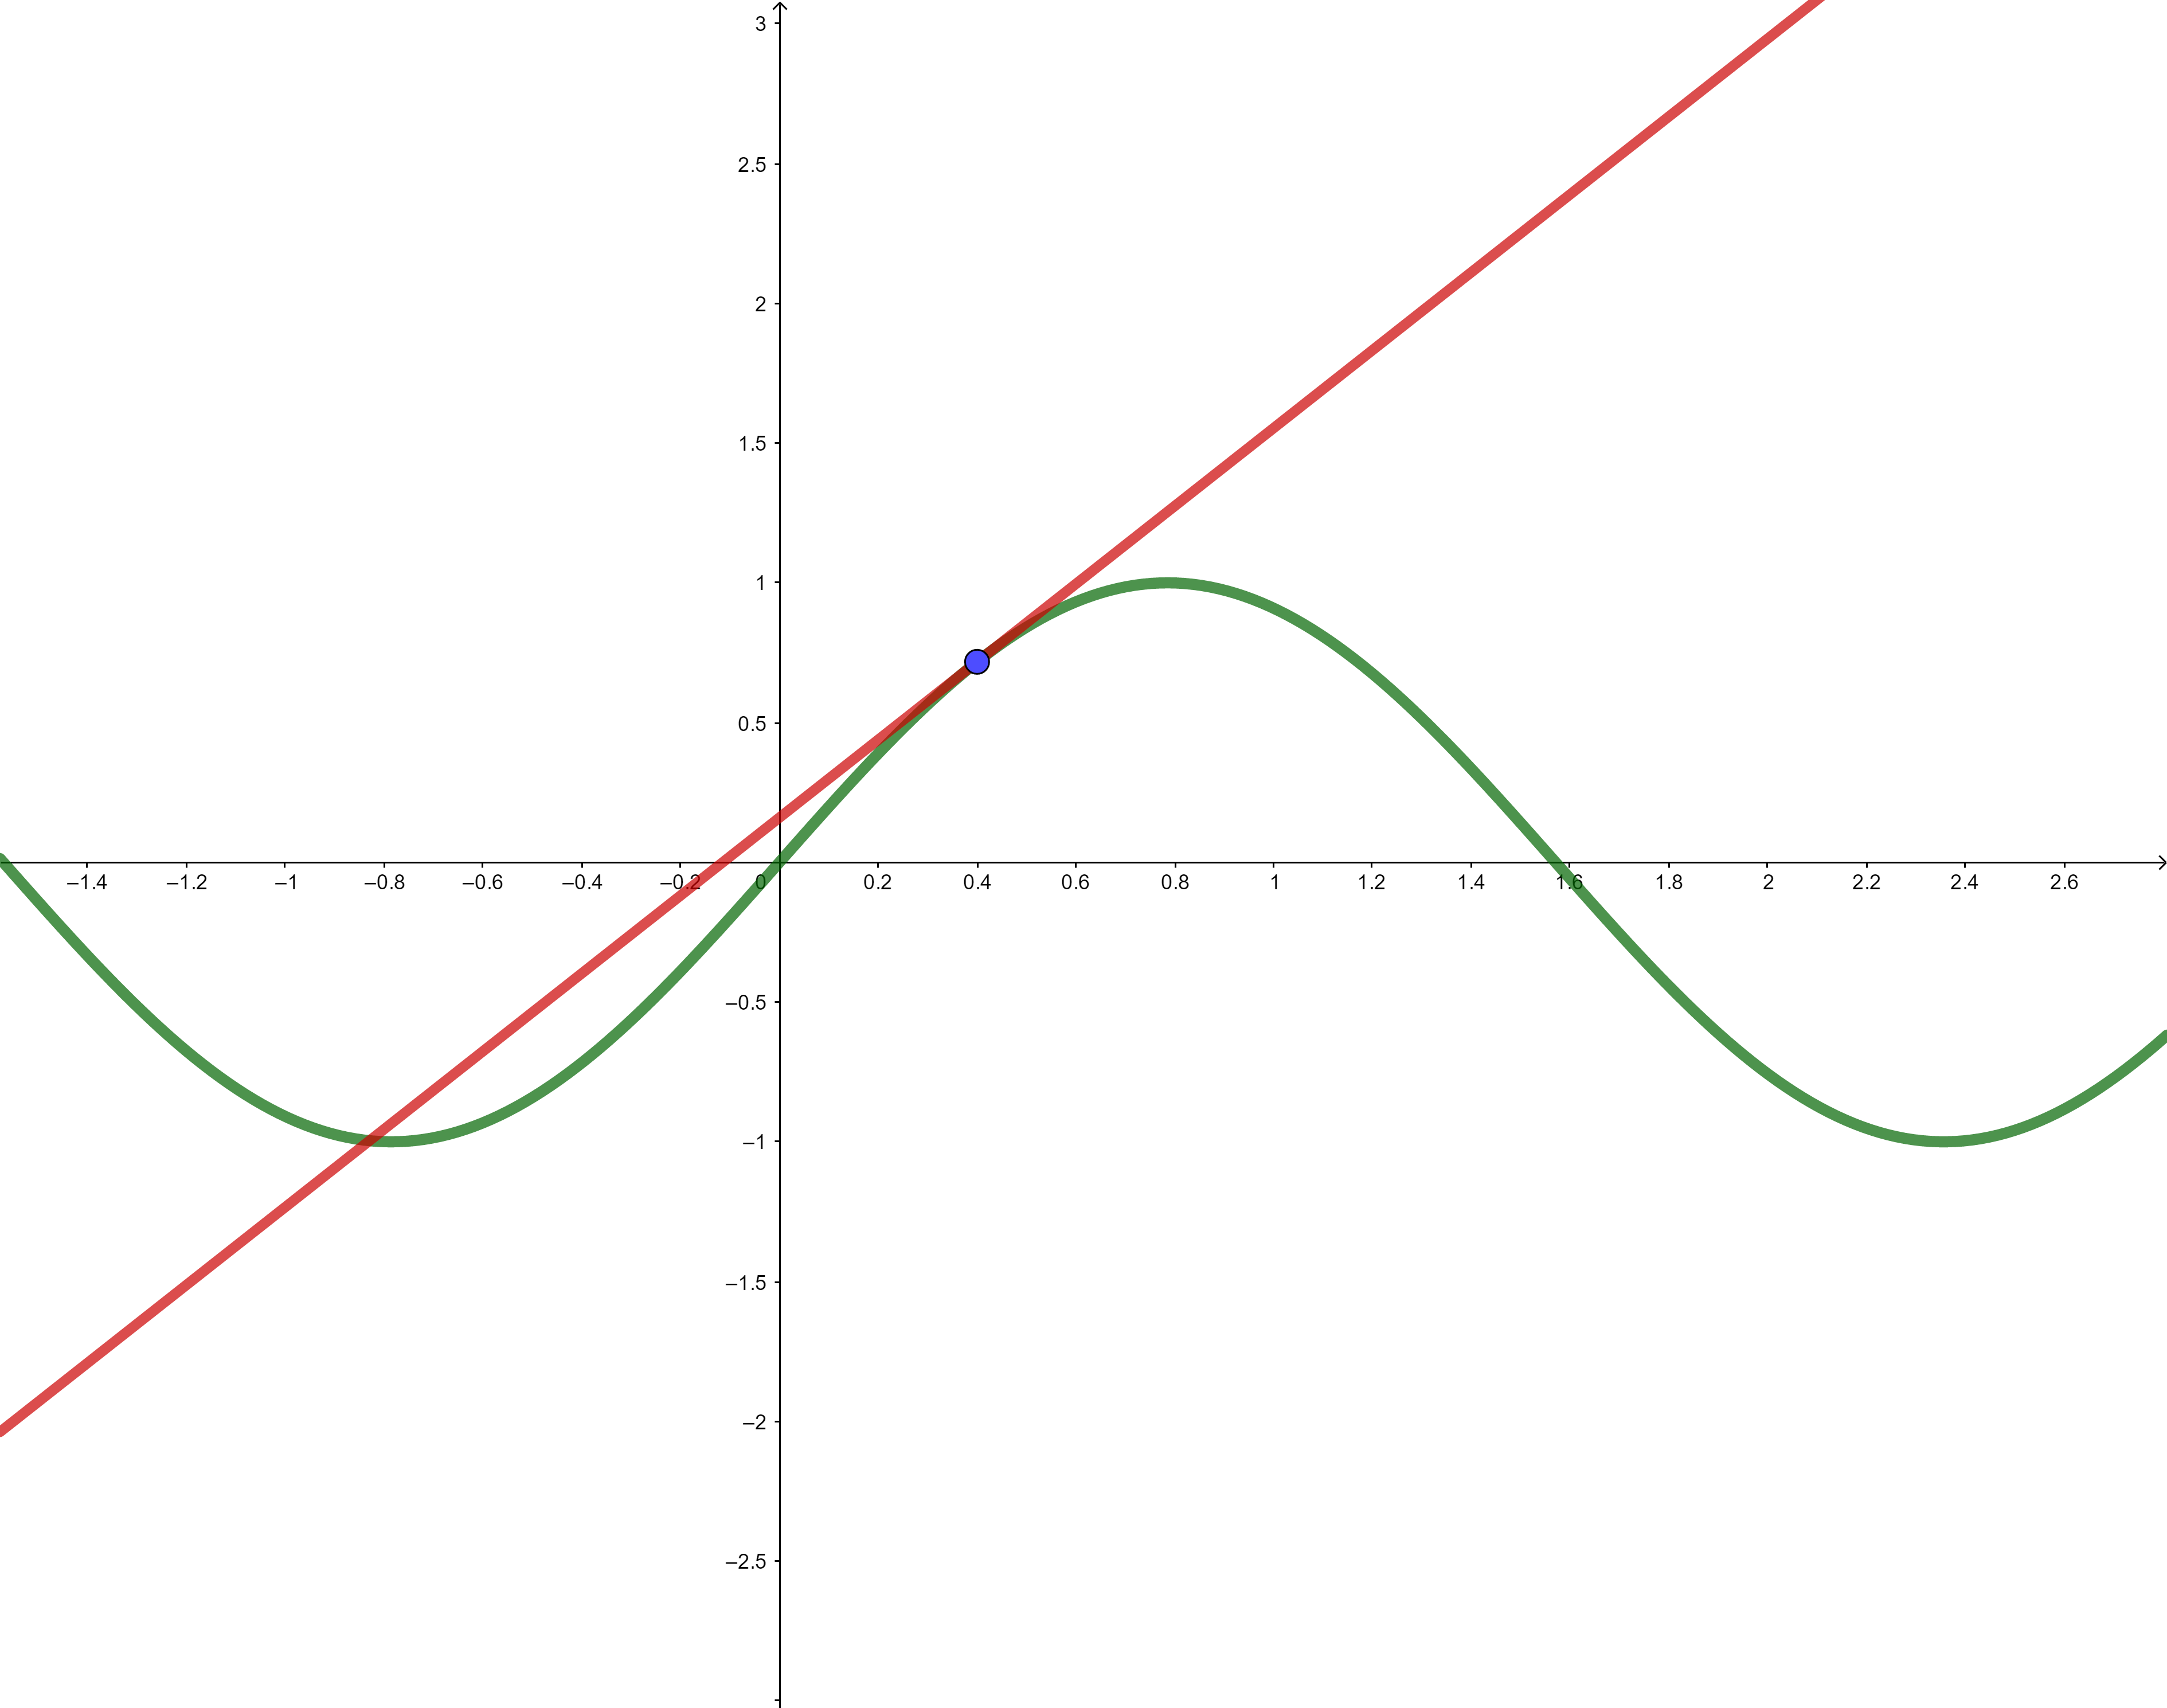
\includegraphics[width=\textwidth]{../Mathematik_2/Bilder/taylor_sinus_tangente.png}
\end{minipage}
	\begin{minipage}{0.6\textwidth}
		F�r $\sin:x\mapsto \sin(x)$ lautet die Tangente in $x_0=2/5$: \[p_1:x\mapsto \sin(2/5) + \cos(2/5)(x-2/5)\]
		Die Tangente erf�llt:
	\begin{itemize}
		\item $p_1(2/5) = \sin(2/5)$ ,
		\item $p_1'(2/5) = \cos(2/5)$.
	\end{itemize}
\end{minipage}
\end{exabox}

F�r eine beliebige differenzierbare Funktion lautet die Tangentengerade an der Stelle $x_0$ also
\[
	p_1(x) =  f(x_0) + f'(x_0)(x-x_0)\,,
\]
und es gilt
\begin{itemize}
	\item $p_1$ l�uft durch den Punkt $(x_0|f(x_0))$, also $p_1(x_0) = f(x_0)$,
	\item $p_1$ hat in $x_0$ dieselbe Steigung wie $f$, also $p_1'(x_0) = f'(x_0)$.
\end{itemize}

Als n�chstes kann man die quadratische Parabel suchen, die sich einer zweimal differenzierbaren Funktion $f$ an einer Stelle $x_0$ am besten ann�hert\footnote{im Sinne einer Interpolation.}: das ist die quadratische N�herung oder auch Schmiegeparabel.
\begin{exabox}{Schmiegeparabel}{ }
	\hspace{-0.3cm}\begin{minipage}{0.4\textwidth}
		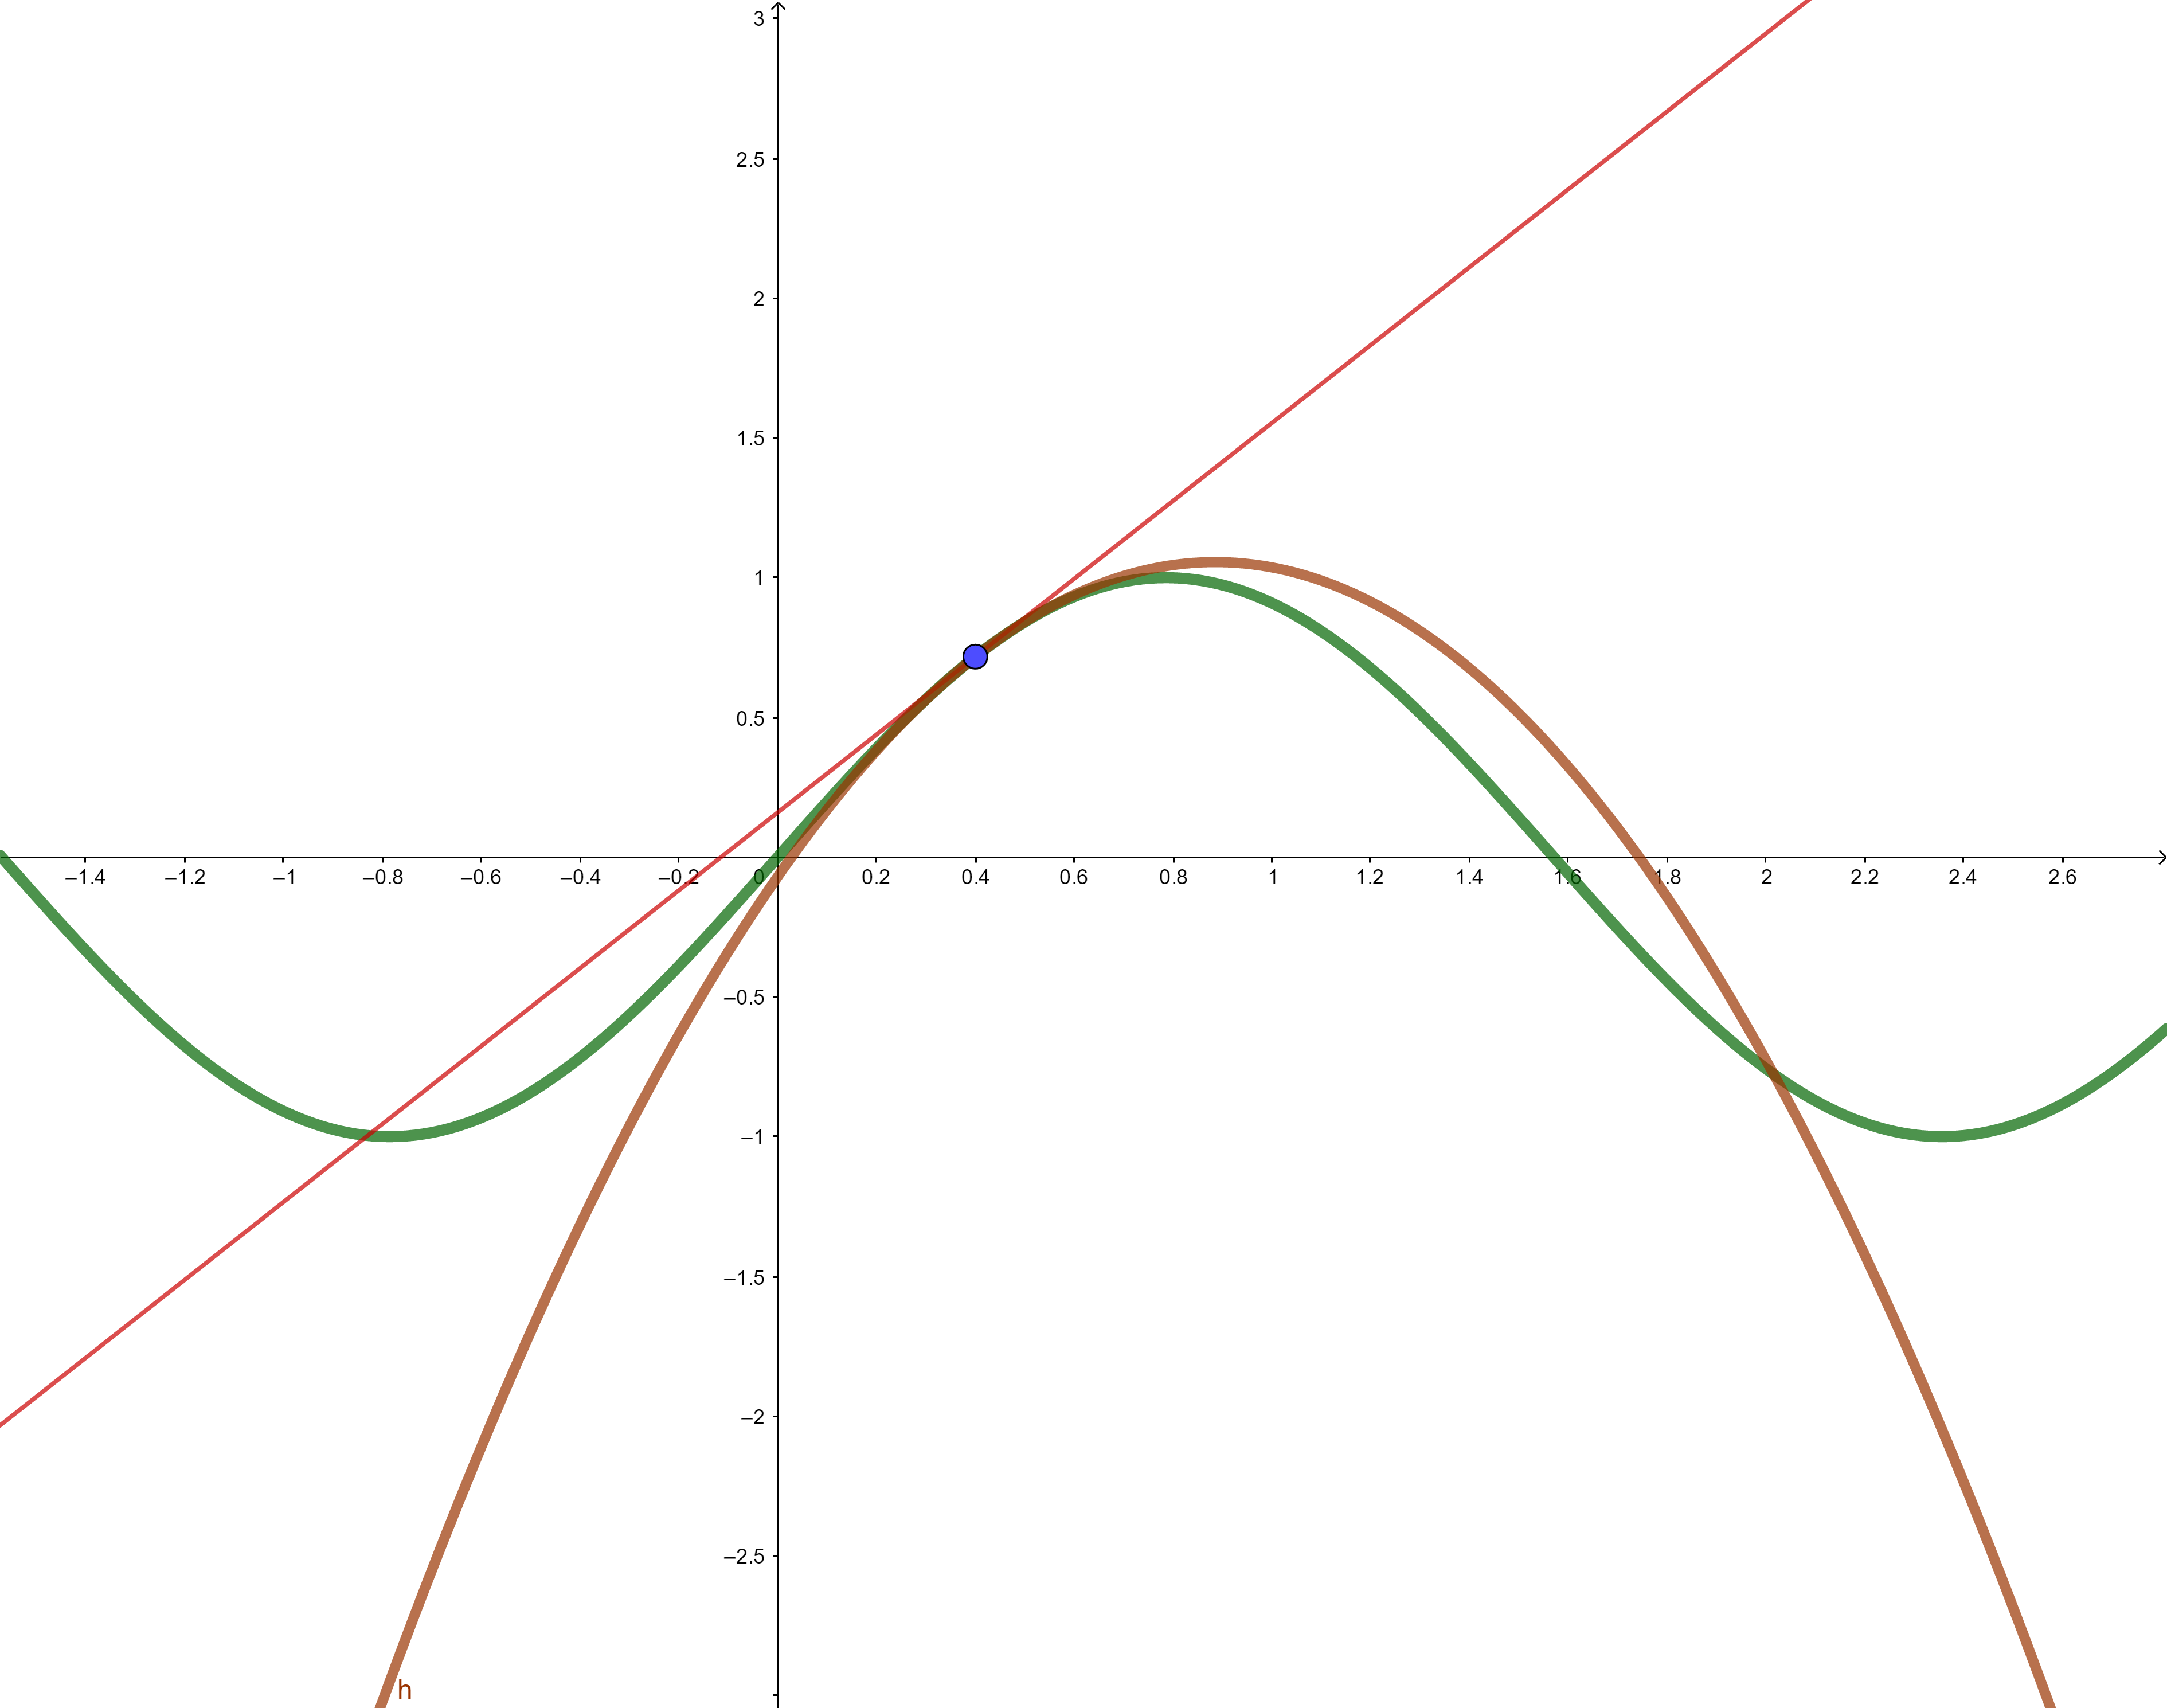
\includegraphics[width=\textwidth]{../Mathematik_2/Bilder/taylor_sinus_schmiegeparabel.png}
\end{minipage}
	\begin{minipage}{0.6\textwidth}
		F�r $\sin:x\mapsto \sin(x)$ lautet die Schmiegeparabel in $x_0=2/5$: \[p_2:x\mapsto \sin(2/5) + \cos(2/5)(x-2/5) - 1/2\sin(2/5)(x-2/5)^2\]
		Die Schmiegeparabel erf�llt:
	\begin{itemize}
		\item $p_2(2/5) = \sin(2/5)$ ,
		\item $p_2'(2/5) = \cos(2/5)$.
		\item $p_2''(2/5) = -\sin(2/5)$.
	\end{itemize}
\end{minipage}
\end{exabox}

F�r eine beliebige zweimal differenzierbare Funktion lautet die Schmiegeparabel an der Stelle $x_0$:
\begin{eqnarray*}
	p_2(x) &=&  f(x_0)+ f'(x_0)(x-x_0) +\frac12 f''(x_0)(x-x_0)^2,
\end{eqnarray*}
und es gilt
\begin{itemize}
	\item $p_2$ l�uft durch den Punkt $(x_0|f(x_0))$, also $p_2(x_0) = f(x_0)$,
	\item $p_2$ hat in $x_0$ dieselbe Steigung wie $f$, also $p_2'(x_0) = f'(x_0)$.
	\item $p_2$ hat $x_0$ dieselbe Kr�mmung wie $f$, also $p_2''(x_0) = f''(x_0)$.
\end{itemize}

Entsprechend  findet  man  die  Formeln  f�r  die beste lokale N�herung durch \underline{Polynome}\randverweis{MA1-polynome} dritten \ldots oder zehnten Grades:
\begin{eqnarray*}
	p_3(x) &=& f(x_0) + f'(x_0)(x-x_0)+ \frac12 f''(x_0)(x-x_0)^2+\frac16 f'''(x_0)(x-x_0)^3\,,\\
	\cdots&&\\
	p_{10}(x) &=& f(x_0) + f'(x_0)(x-x_0)+ \frac12 f''(x_0)(x-x_0)^2+ \cdots + \frac{1}{10!} f^{(10)}(x_0)(x-x_0)^{10}\,.
\end{eqnarray*}

\begin{exabox}{Taylor-Polynom vom Grad $10$}{ }
	\begin{center}
	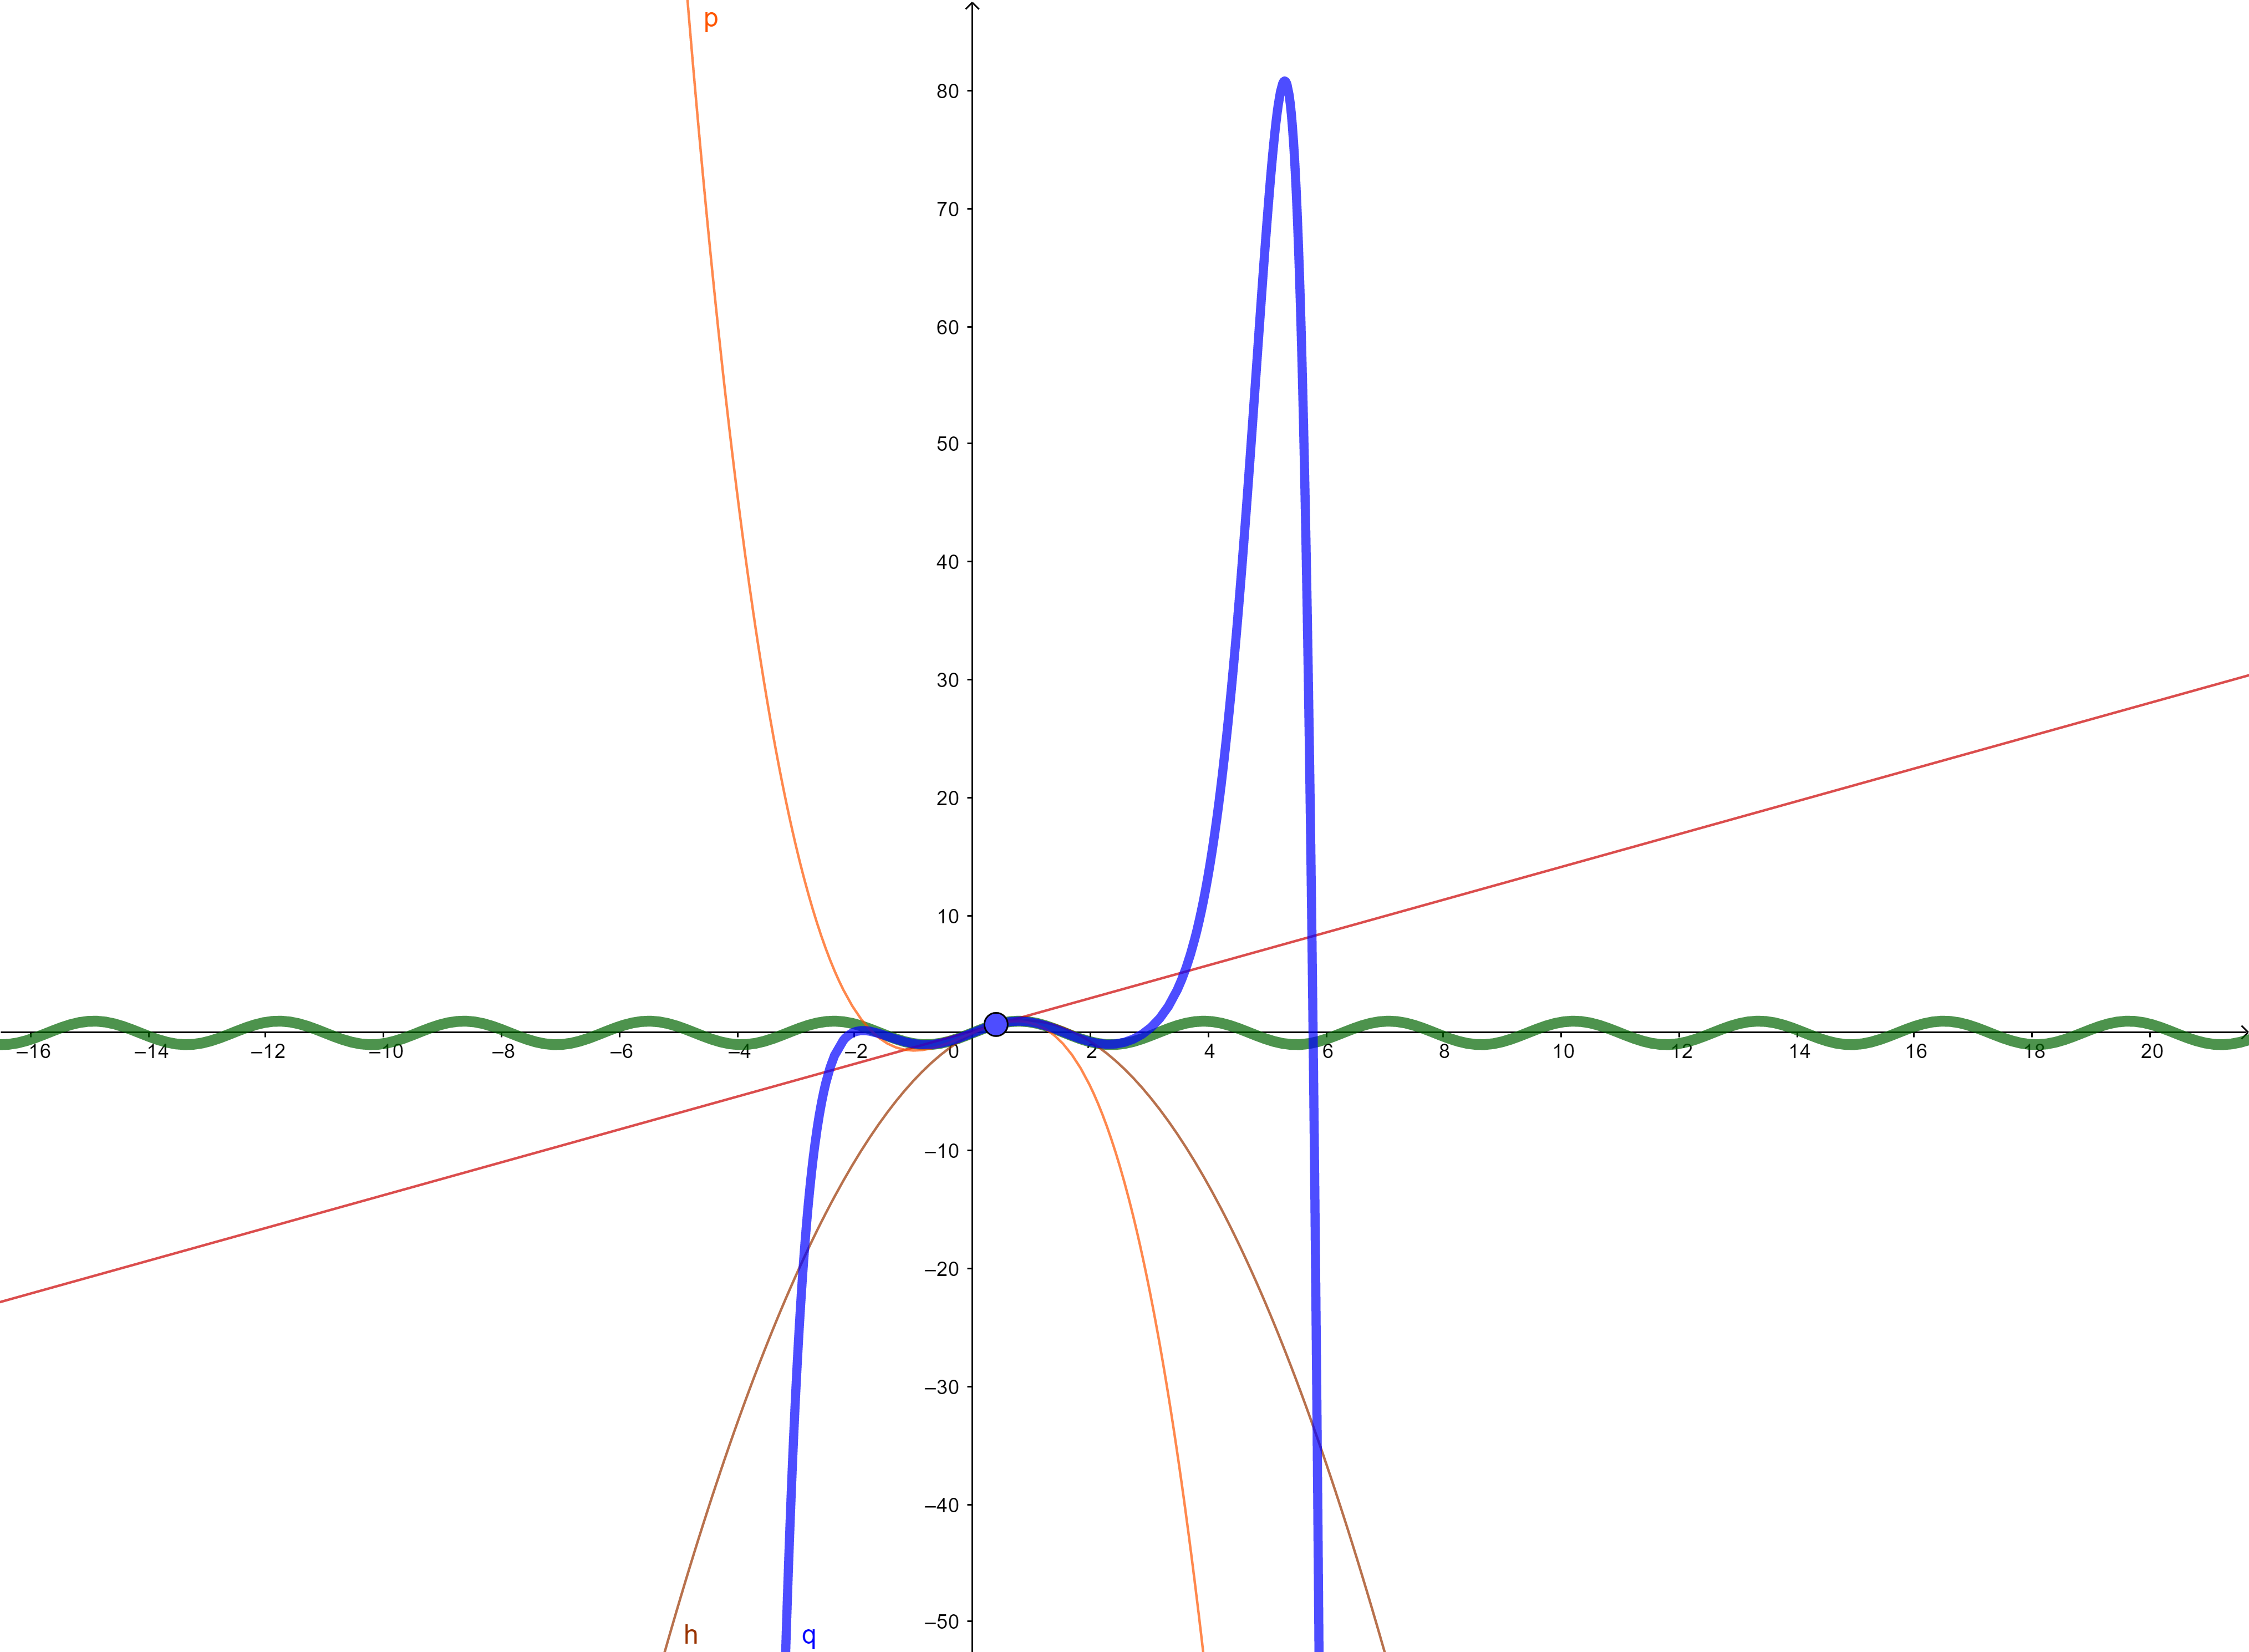
\includegraphics[width=0.7\textwidth]{../Mathematik_2/Bilder/taylor_sinus_polynom_grad_10.png}
\end{center}
\end{exabox}
Vorausgesetzt die Funktion $f$ besitzt mindestens Ableitungen bis zur Ordnung $n$, dann kann man auf diese Weise ein Polynom $p_n$ vom Grad $n$ entwickeln, das sogenannte Taylor-Polynom vom Grad $n$:
\begin{defbox}{Taylor-Polynom vom Grad $n$}{ }
	F�r eine $n$-mal differenzierbare Funktion lautet das Taylor-Polynom vom Grad $n$:

	\begin{eqnarray*}
		p_n(x) &=& f(x_0) + f'(x_0)(x-x_0) + \frac12 f''(x_0)(x-x_0)^2 + \cdots + \frac{1}{n!} f^{(n)}(x_0)(x-x_0)^n \\
		&=& \sum\limits_{k=0}^{n}\frac{1}{k!}f^{(k)}(x_0)(x-x_0)^k\,.
\end{eqnarray*}
Das Taylorpolynom $p_n$ stimmt an der Stelle $x=x_0$ mit der Funktion $f$ und mit deren Ableitung bis zum Grad $n$ �berein:
\[ \forall\, k=0,\cdots,n: \quad p_n^{(k)}(x_0)= f^{(k)}(x_0)\,.  \]
\end{defbox}

\noindent Bemerkungen:\marginpar{\small Aufgaben}
\begin{itemize}
	\item In der Praxis ist nur das lokale Verhalten einer Funktion oder Kennlinie interessant. Um die Analyse zu erleichtern kann man anstatt der Orginalfunktion ein Taylorpolynom betrachten!
	\item Das \underline{asymptotische Verhalten}\randverweis{MA1-ableitungen-und-funktionsverlauf} des Taylorpoynoms entspricht dem des Polynoms und kann unter Umst�nden ganz anders sein als das der betrachteten Funktion!
	\item Wechselt man den Entwicklungspunkt $x_0$, muss man das Taylorpolynom neu bestimmen.
\end{itemize}

Im folgenden Beispiel wird die Wurzelfunktion an der Stelle $x_0 = 4$ mit einem Taylorpolynom vom Grad $3$ angen�hrt:
\begin{exabox}{Taylor-Polynom an $f:x\to\sqrt{x}$ vom Grad $n=3$ an $x_0=4$}{ }
Bestimmung der Ableitungen bis zum Grad $3$:
\begin{eqnarray*}
		f(x) &=& \sqrt{x} = x^{1/2}\,,\\[1ex]
		f'(x) &=& \frac12 x^{-1/2} = \frac12 \frac{1}{\sqrt{x}}\,,\\[1ex]
		f''(x) &=& -\frac14 x^{-3/2} =- \frac14 \frac{1}{\sqrt{x}^3}\,,\\[1ex]
		f'''(x) &=& \frac38 x^{-5/2} =- \frac38 \frac{1}{\sqrt{x}^5}\,.
	\end{eqnarray*}

L�sung $p_3$ mit $x_0=4$:
	\[
	p_3:\mathbb R \to \mathbb R, x\mapsto 2 + \frac14(x-4)- \frac{1}{32} \frac{1}{2} (x-4)^2 + \frac{3}{256} \frac{1}{6} (x-4)^3\,.
\]
\begin{center}
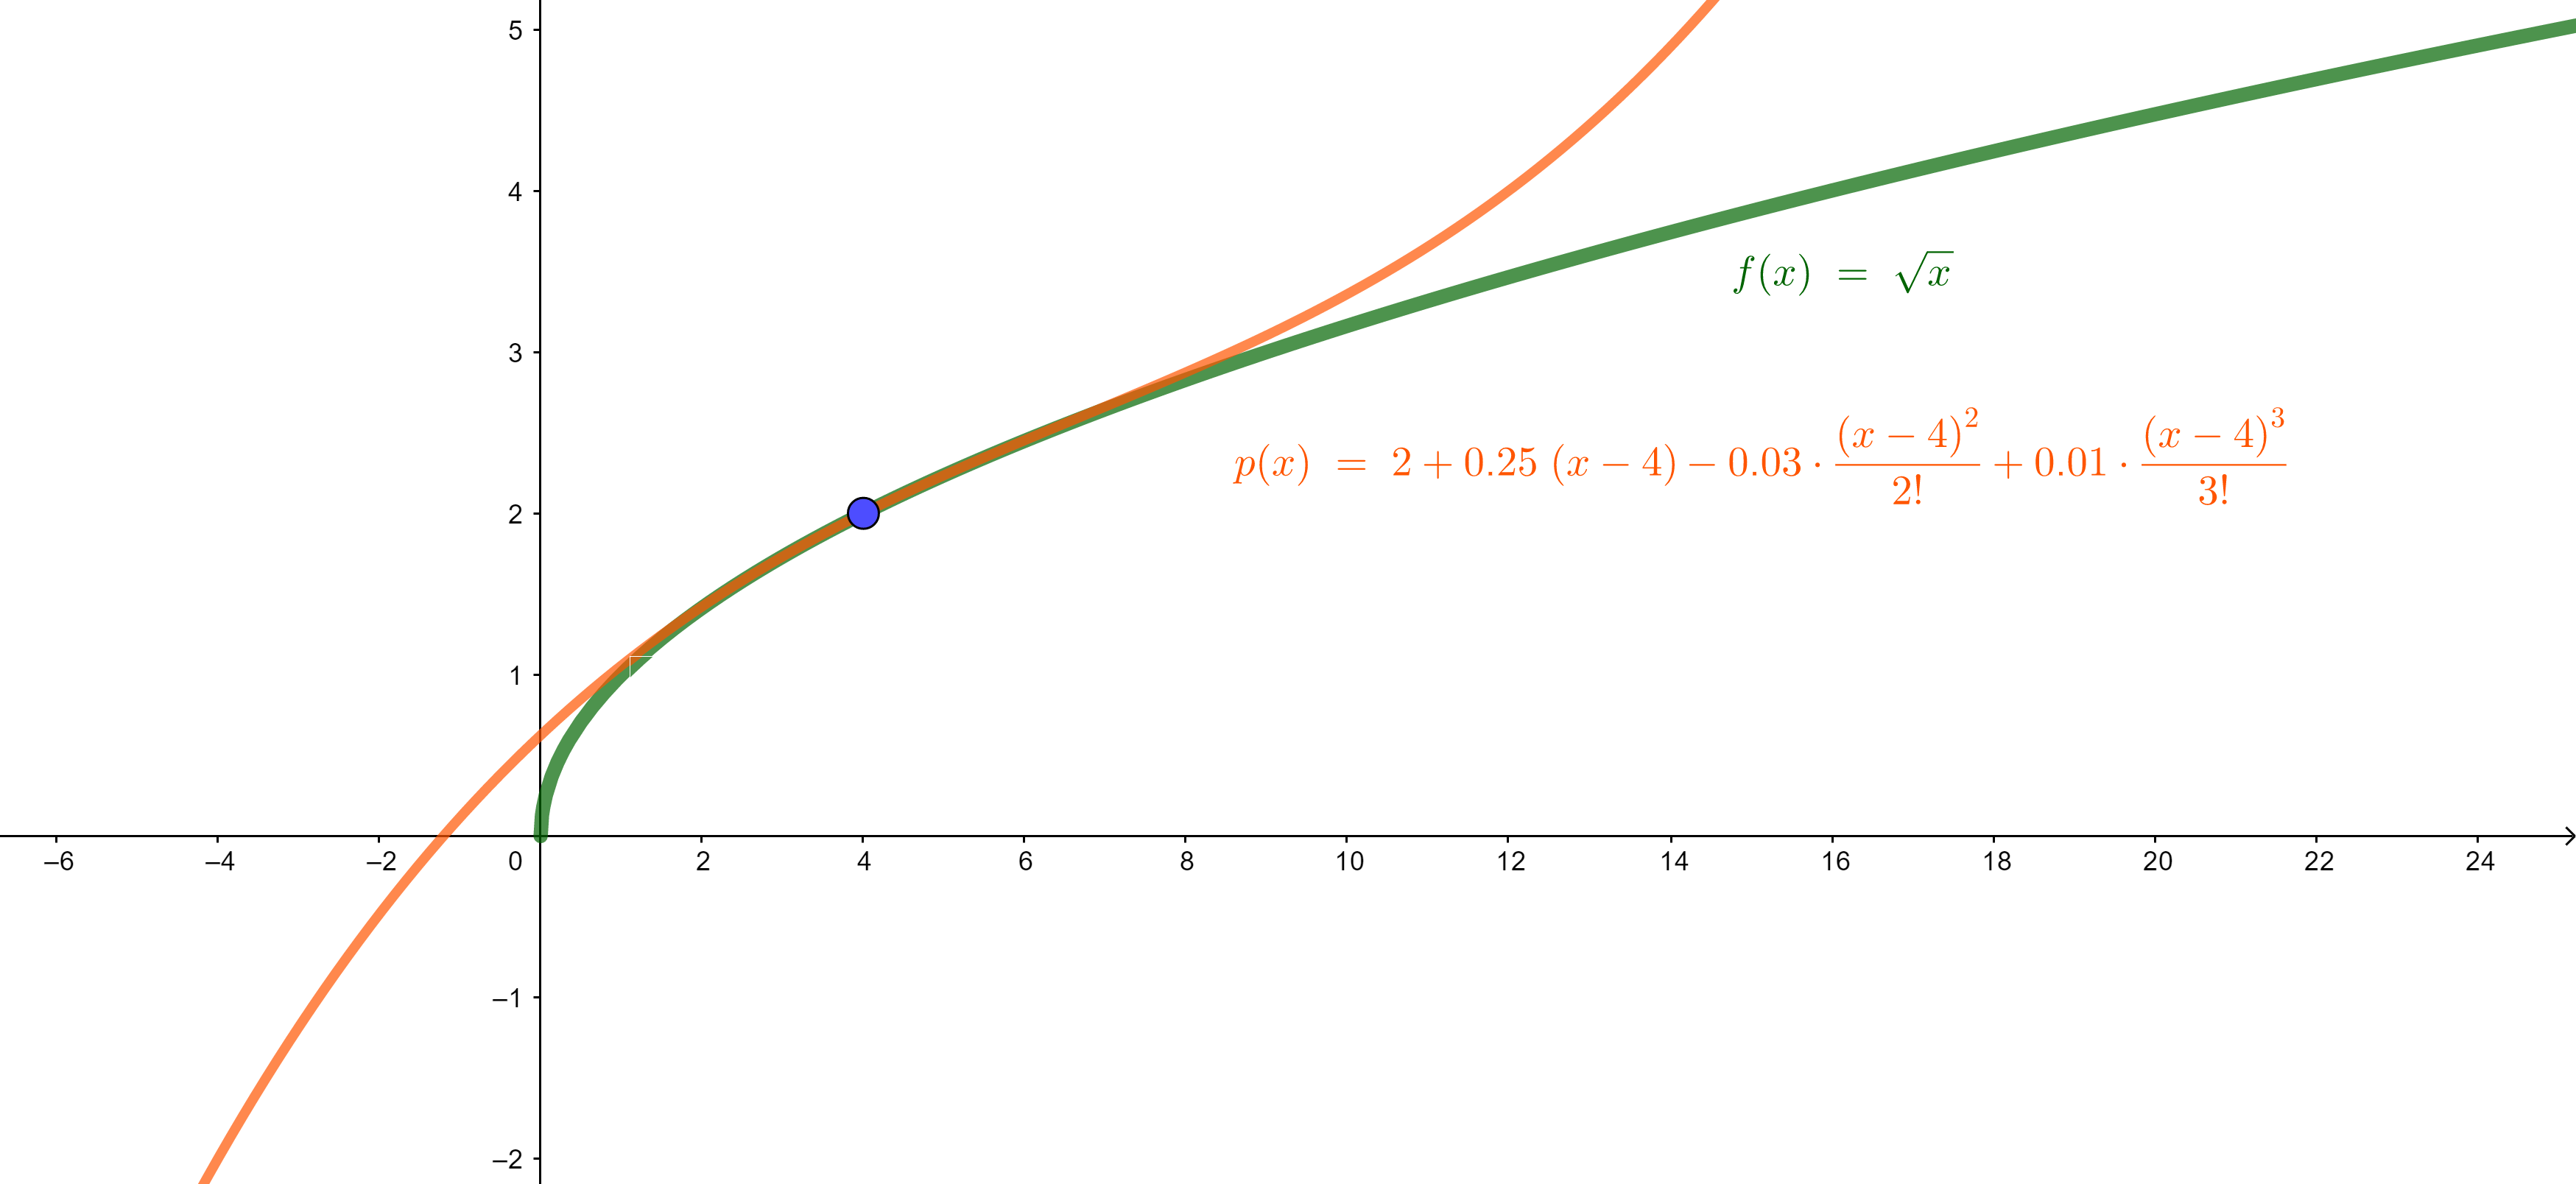
\includegraphics[width=0.7\textwidth]{../Mathematik_2/Bilder/taylor_wurzelfunktion_polynom_grad_3.png}
\end{center}
\end{exabox}

 \newpage % 02 Taylorpolynome
\setcounter{def}{0} \setcounter{satz}{0} \setcounter{exa}{0} \section{Taylor-Reihe}\label{MA2-taylorreihen}

\begin{table}[H]
  \centering
  \begin{tabularx}{\textwidth}{@{}>{\raggedright\arraybackslash}X r@{}}
    \toprule
    \multicolumn{2}{c}{\textbf{�bersicht �ber Lernziele und Voraussetzungen}}\\
    \midrule
    \textbf{Lernziele} & \\[.5\normalbaselineskip]
    \tabitem eine Taylor-Reihe formal angeben  & \\
    \tabitem eine Potenz-Reihe als Funktion interpretieren (Einsetzen von $x$ liefert Zahlenreihe) & \\
    \tabitem entscheiden, ob eine Taylor-Reihe die ihr zugrunde liegende Funktion darstellt & \\
    \tabitem den Approximationsfehler $R_n(x)=f(x)-p_n(x)$ absch�tzen und interpretieren (+) & \\[.5\normalbaselineskip]
    \midrule
    \textbf{Voraussetzungen} & \\[.5\normalbaselineskip]
    \tabitem wichtige Zahlenreihen & \abschnittsverweis{MA2-zahlenreihen} \\
    \tabitem Ableitungen (inkl.\ h�herer Ableitungen) bilden & \abschnittsverweis{MA1-ableitungsregeln} \\
    \tabitem Ungleichungen l�sen und Absch�tzungen umformen & \abschnittsverweis{MA1-aequivalenzumformungen} \\[.5\normalbaselineskip]
    \bottomrule
  \end{tabularx}
\end{table}

\noindent \ifintegriereaufgaben Die �bungsaufgaben zum Thema finden Sie \hyperref[MA2-taylorreihen-aufgaben]{hier}.
\vspace{0.3cm}
\hrule
\fi

F�r eine unendlich oft differenzierbare Funktion, kann man die N�herung durch Polynome immer weiter verbessern\footnote{im Sinne einer lokalen Approximation!} und gelangt damit formal zur Taylor-Reihe [Taylor series]:
\begin{defbox}{Taylor-Reihe}{}
	Eine unendlich oft differenzierbare Funktion l��t sich formal an jedem Punkt $x_0 \in D_f$ in eine Taylor-Reihe entwickeln:
	\[
	Tf(x,x_0): =  f(x_0) + f'(x_0)(x-x_0) + \cdots + \frac{f^{(n)}(x_0)}{n!}(x-x_0)^n + \cdots = \sum\limits_{k=0}^\infty \frac{f^{(k)}(x_0)}{k!}(x-x_0)^k \,.\]
\end{defbox}

\noindent Bemerkungen:
\begin{itemize}
	\item Die Struktur einer Taylor-Reihe ist anders als diejenige der unendlichen Reihen, die wir im vorangegangenen Kapitel\randverweis{MA2-zahlenreihen} kennengelernt haben.
	\item Anstatt Zahlen aufzuaddieren, werden hier Potenzen von $x$, also Funktionen, aufaddiert!
	\item Fixiert man ein $x\in D_f$, und setzt es in die Reihe ein, dann erh�lt man eine unendliche Reihe nach dem Schema des letzten Abschnitts. Beispielsweise f�r $x=3, x_0=0$:
		\[
	\sum\limits_{k=0}^\infty \frac{f^{(k)}(0)}{k!}3^k = \sum\limits_{k=0}^\infty a_k, \quad a_k := \frac{f^{(k)}(0)}{k!}3^k \in \mathbb R  \,.
\]
\item Eine unendliche Reihe, in der Potenzen von $x$ aufsummiert werden - garniert mit einem Koeffizienten - bezeichnet man Potenzreihen
	\[
		\sum\limits_{k=0}^\infty c_k x^k \,.
	\]
	Taylor-Reihen sind also spezielle Potenzreihen.
	\end{itemize}

Zwei Fragen stellen sich:
\begin{itemize}
	\item Gibt es $x \in D_f$, f�r die die Taylor-Reihe \underline{konvergieren}\randverweis{MA2-zahlenreihen}?
	\item Wenn wir ein $x \in D_f$ identifiziert haben, f�r das die Taylor-Reihe konvergiert, gilt dann Gleichheit, also: $\forall \, x\in D_f:\quad Tf(x,x_0) = f(x)$?
\end{itemize}
Klar ist: falls wir Bedingungen kennen, unter denen sich die Fragen mit ja beantworten lassen, dann bedeutet das einen enormen Gewinn, denn $f$, egal wie kompliziert, wird pl�tzlich einfach berechenbar. Es lohnt sich also auf diese Fragen einzugehen und das werden wir in den n�chsten Abschnitten tun. F�r den Moment konzentrieren wir uns noch auf das Erlernen des Handwerkszeugs: wir entwickeln Taylor-Reihen!

\begin{exabox}{Taylor-Reihe f�r $f: x\mapsto \exp(x)$ }{ }
	Funktion: \[ f: \mathbb R \to (0,\infty),  x\mapsto e^x \]
	Entwicklungspunkt:
	\[ x_0 \in \mathbb R : \; x_0 = 0\,.\]
	Ableitungen:
\[
	\forall\, k\in \mathbb N_0:\quad f^{(k)}(x) = e^x \Rightarrow  	f^{(k)}(0) = 1\,.
\]
	Taylor-Reihe mit $x_0=0$:
	\[
	Tf(x,0):=1 + x + \cdots + \frac{1}{n!}x^n + \cdots = \sum\limits_{k=0}^\infty \frac{1}{k!}x^k \,.
\]
\end{exabox}

\begin{exabox}{Taylor-Reihe f�r $f: x\mapsto \exp(ix)$ }{ }
	Funktion: \[ f: \mathbb R \to \mathbb C, x \mapsto e^{ix} \]
	Entwicklungspunkt:
	\[ x_0 \in \mathbb R :\; x_0 = 0\,.\]
	Ableitungen\dots
\[
	\forall\, k\in \mathbb N_0:\quad f^{(k)}(i x) = i^k e^{i x} \Rightarrow  	f^{(k)}(0) = i^k\,.
\]
	Taylor-Reihe mit $x_0=0$:
\[ Tf(x,0):=1 + \cdots + \frac{i^n}{n!}x^n + \cdots = \sum\limits_{k=0}^\infty \frac{i^k}{k!}x^k \,.\]
\end{exabox}

\noindent Bemerkungen:\marginpar{\small Aufgaben}
\begin{itemize}
	\item Um eine N�herung beispielsweise an die Zahl $e^{1/2}$ anzugeben, summeriert man die ersten f�nf bis zehn Summanden dieser Reihe auf.
	\item Entsprechend betrachtet man eine Talyor-Reihe f�r ein komplexes Argument $z=x+iy$ und kann eine N�herung von $e^{3+4i}$ angeben.
\end{itemize}

Die \underline{Eulersche Identit�t}\randverweis{MA1-komplexe-zahlen-polarform-und-euler}
\[
	re^{i\varphi} = r ( \cos(\varphi) + i\sin(\varphi) )\,.
\]
er�ffnet einen Weg, um von der komplexen Exponentialfunktion zu den \underline{trigonometrischen Funktionen}\randverweis{MA1-trigonometrische-funktionen} zu gelangen. Die Taylor-Reihen f�r Sinus und Kosinus sind folgende Potenzreihen:
\begin{exabox}{Taylor-Reihe f�r $f_1:x\mapsto \sin(x)$ und $f_2:x\mapsto \cos(x)$}{ }
	Funktionen:
	\[\begin{cases}
			f_1: &\mathbb R \to \mathbb R, x\mapsto \sin(x) \\
			f_2: &\mathbb R \to \mathbb R, x\mapsto \cos(x) \\
		\end{cases}
	\]
	Ableitungen:
	\begin{center}
		\begin{tabular}{c|c c c c c c c c c c }
			& $f(0)$ & $f{(1)}(0)$ & $f^{(2)}(0)$ & $f^{(3)}(0)$ &$f^{(4)}(0)$ & $f^{(5)}(0)$ & $f^{(6)}(0)$ & $f^{(7)}(0)$ &  \ldots \\
			\hline
			$\sin$ & $0$ & $1$ & $0$ &  $-1$ & $0$ & $1$ & $0$ &  $-1$ &\ldots \\
			$\cos$ & $1$ & $0$ & $-1$&  $0$ & $1$ & $0$ & $-1$&  $0$ &\ldots
		\end{tabular}
	\end{center}
	Taylor-Reihen mit $x_0=0$:
	\begin{eqnarray*}
		\begin{cases}
			Tf_1(x,0)=  x - \displaystyle{\frac{1}{3!}} x^3 + \displaystyle{\frac{1}{5!}} x^5 -+  \cdots = \displaystyle{\sum\limits_{k=0}^\infty} (-1)^{k} \displaystyle{\frac{1}{(2k+1)!}} x^{2k+1} \,,\\[1ex]
			Tf_2(x,0) =  1 - \displaystyle{\frac12} x^2 + \displaystyle{\frac{1}{4!}} x^4 - \displaystyle{\frac{1}{6!}} x^6 +-  \cdots = \displaystyle{\sum\limits_{k=0}^\infty} (-1)^{k}\displaystyle{\frac{1}{(2k)!}} x^{2k} \,.
		\end{cases}
	\end{eqnarray*}
%Betrachtet man nur die ersten $n$ Summanden, erh�lt man Taylor-Polynome, die sich mehr und mehr um die $x$-Achse wickeln, um sich dann entsprechen $x^n$ asymptotisch Unendlich ann�hern:
	\centering
	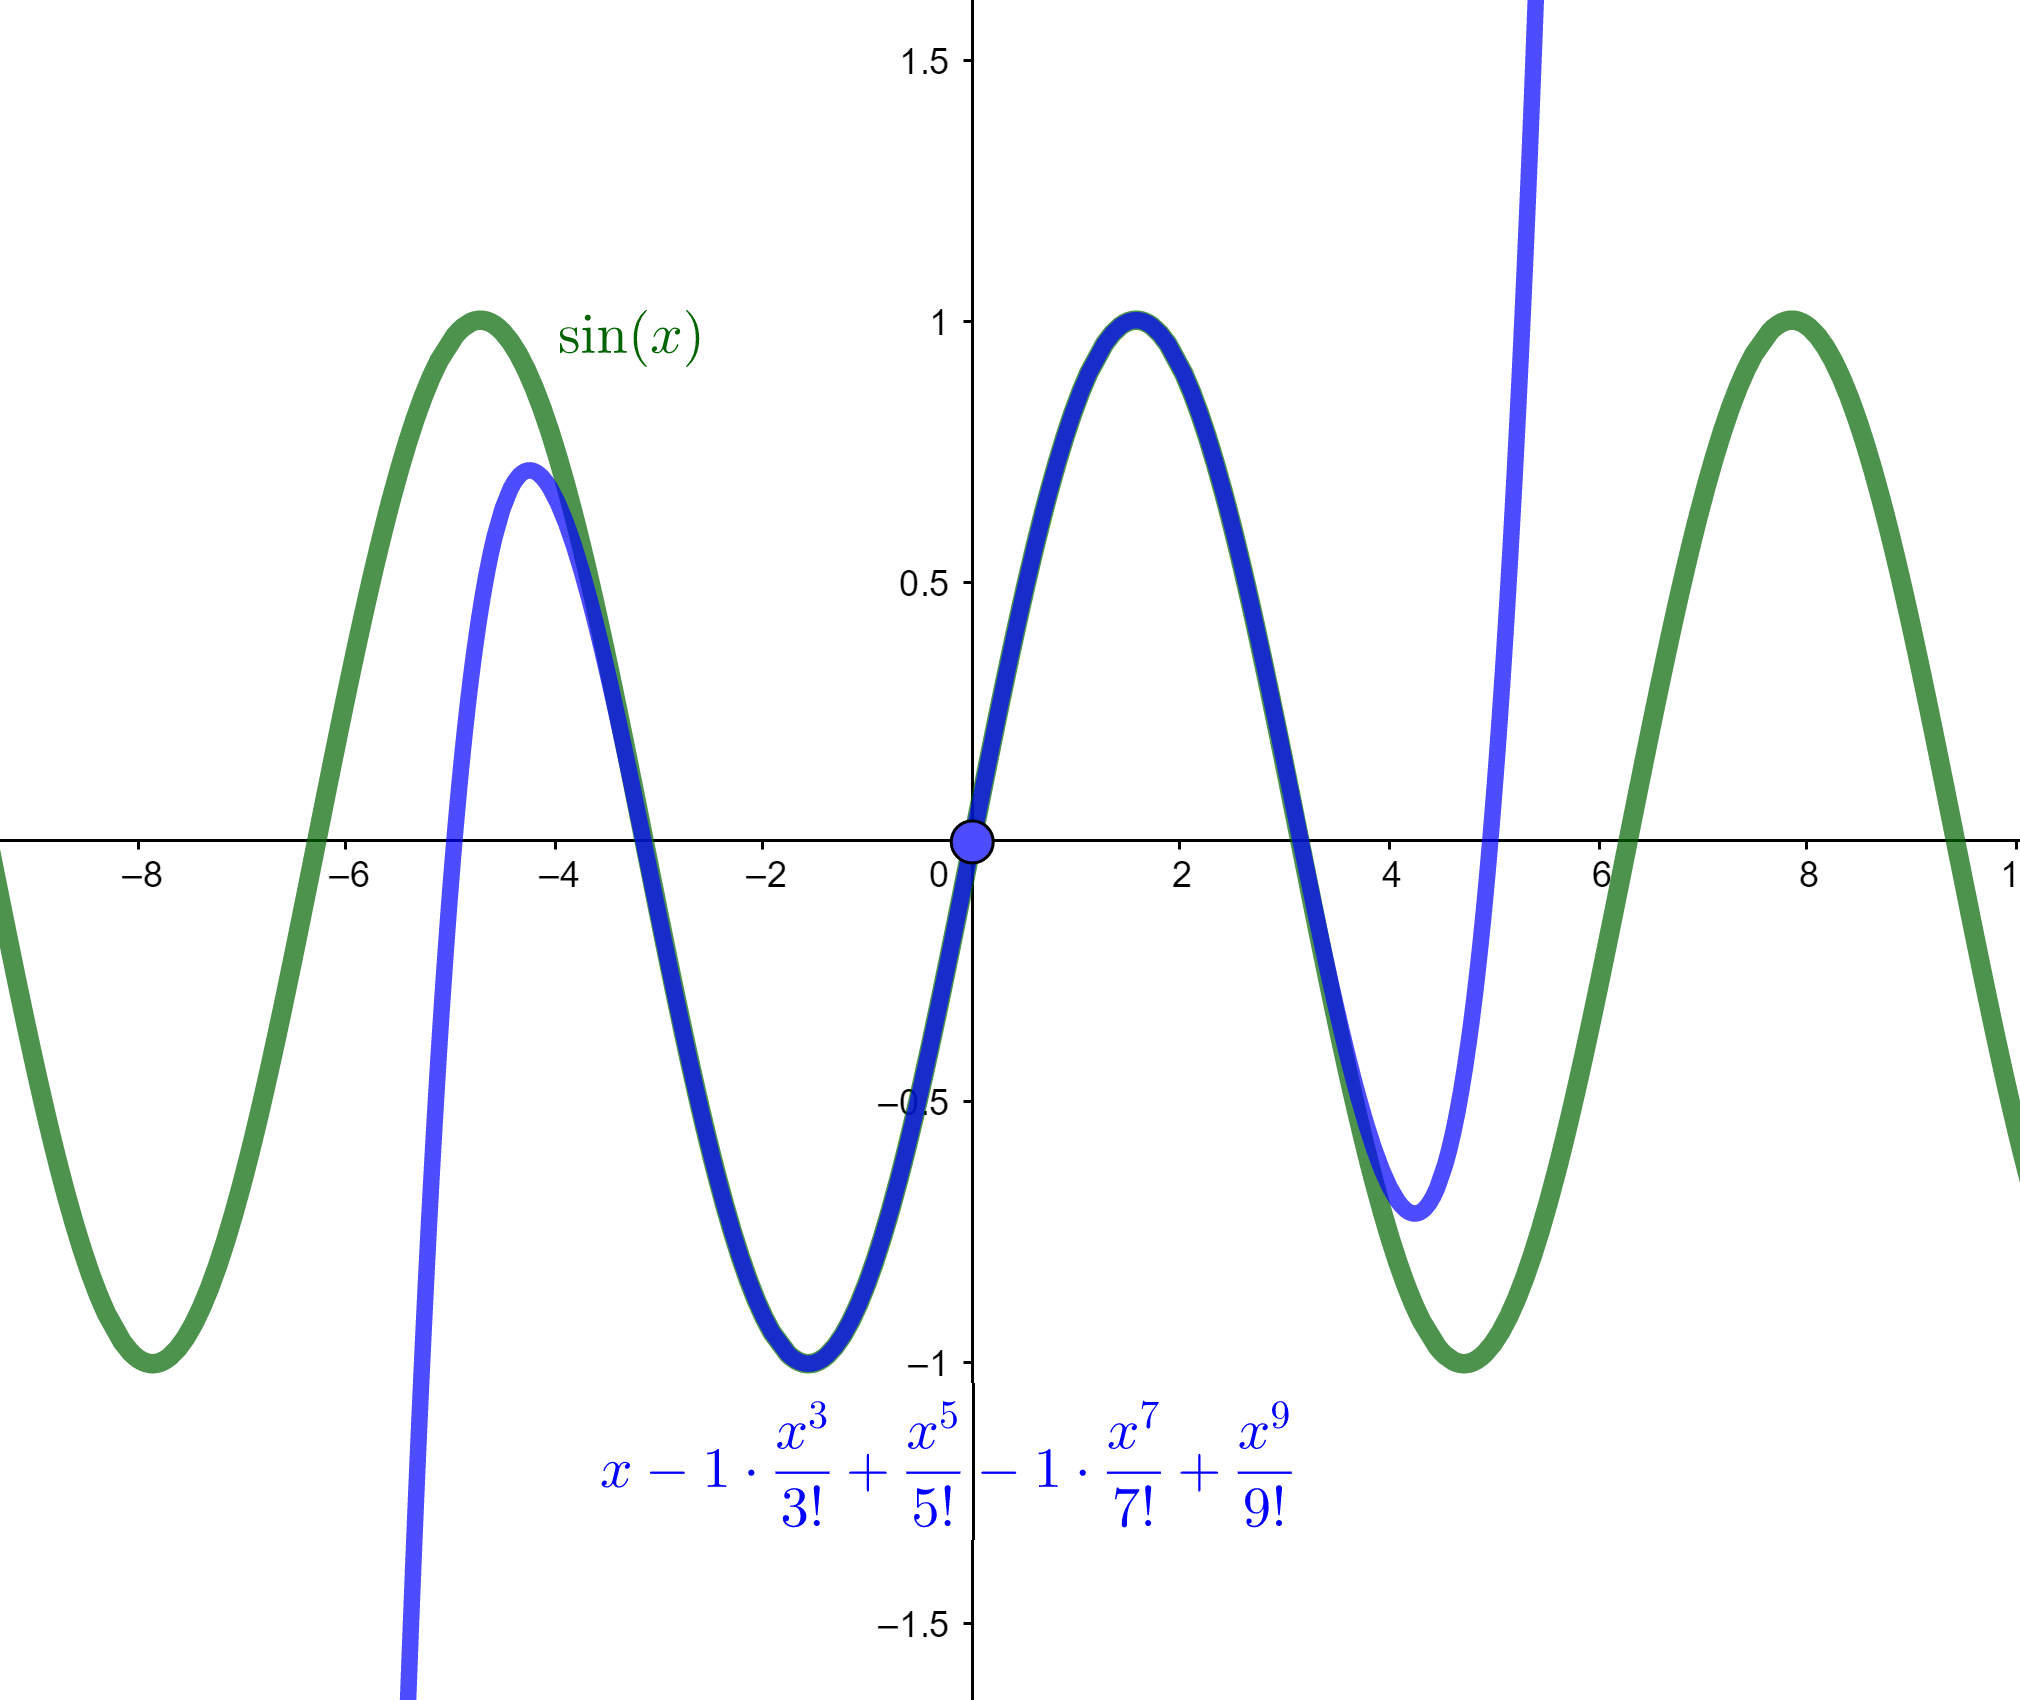
\includegraphics[width=0.6\textwidth]{../Mathematik_2/Bilder/taylor_sinus_maclaurinpolynom_grad_10.png}
\end{exabox}
%Demo mit Wolfram Alpha: \begin{verbatim} series sin(x) at x=0 order 20 \end{verbatim} Durch Einsetzen von $x=i \varphi$ in die Potenzreihe f�r die Exponentialfunktion findet man:

Als n�chstes Beispiel entwickeln wir die \underline{gebrochenrationale Funktion}\randverweis{MA1-rationale-funktionen} $f: x\mapsto 1/(1-x)$ an der Stelle $x_0=0$.

Dazu sind die Ableitungen dieser Funktion zu bestimmen und an der Stelle \(x_0=0\) auszuwerten:
\begin{exabox}{Taylor-Reihe f�r $f:x\mapsto 1/(1-x)$}{ }
	Funktion: \[ f: \mathbb R\setminus\{ 1\} \to \mathbb R, x \mapsto \frac{1}{1-x} \]
	Ableitungen:
	\begin{center}
		\begin{tabular}{cccccc}
			$f(x)$ & $f^{(1)}(x)$ & $f^{(2)}(x)$ & $f^{(3)}(x)$ &  \ldots & $f^{(n)}(x)$\\
			\hline
			$(1-x)^{-1}$ & $(1-x)^{-2}$ & $2(1-x)^{-3}$ & $6(1-x)^{-4}$ & \ldots & $n!(1-x)^{-n-1}$
		\end{tabular}
	\end{center}
	Taylor-Reihe mit $x_0=0$:
	\begin{eqnarray*}
		Tf(x,0) = \frac{1}{1-x} =  1 +x + 2\frac{1}{2!} x^2 + 3!\frac{1}{3!} x^3 \cdots  + n!\frac{1}{n!} x^n + \cdots = \sum\limits_{k=0}^\infty x^{k} \,. \quad(**)
	\end{eqnarray*}
\end{exabox}

\noindent Bemerkungen:
\begin{itemize}
	\item Benutzt man die Tayplor-Reihen zur Darstellung von $\sin$ und $\cos$, so ist  $x$  im Bogenma� einzusetzen, denn die Ableitungen von Sinus und Cosinus bildet man typischerweise im Bogenma�!
	\item Die Taylor-Reihen, die wir f�r die Exponentialfunktion entwickelt haben, kennen wir schon und wir wissen auch schon, dass die Taylor-Reihe die Exponentialfunktion f�r jedes $x\in \mathbb K$ mit $\mathbb K = \mathbb R$ oder $\mathbb C$ darstellt! Das Thema Konvergenz scheint hier kein Problem zu sein.
	\item Bei $(**)$ sieht das anders aus, wie folgendes Experiment zeigt: multiplizieren wir die Partialsumme $1+x+x^2+x^3+\dots + x^n$ mit $(1-x)$, dann erhalten wir \marginpar{\small {Aufgabe}}:
\begin{eqnarray*}
\left( 1 + x + x^2 + \cdots + x^n\right) \cdot (\textcolor{blue}{1}\textcolor{brown}{-x}) &=& \textcolor{blue}{ 1+ x + x^2 + \cdots + x^n}\textcolor{brown}{  -  x - x^2 - x^3 - \cdots - x^{n+1}} \\
&=& \textcolor{blue}{1} \textcolor{brown}{- x^{n+1} }\\[1ex]
 \stackrel{\displaystyle{x\not=1}}{\Rightarrow}  && 1+x+x^2 + \cdots + x^n = \frac{1-x^{n+1}}{1-x} \,.
\end{eqnarray*}
 %eine Teleskopsumme [telescope sum}

Der Term auf der rechten Seite des letzten Gleichheitszeichen entspricht also f�r $n\to \infty$ der Taylor-Reihe $(**)$.
\[
	\lim\limits_{n\to\infty} \left( 1 + x + x^2 + x^3 + \cdots + x^n\right) = \lim\limits_{n\to\infty} \frac{1-x^{n+1}}{1-x} = \textnormal{?}
\]
Die Konvergenz der Reihe muss also ma�geblich von dem Wertebereich von $x$ abh�ngen, denn
\begin{eqnarray*}
	\big|x^{n+1}\big|  \to \begin{cases}  \infty, \quad &|x| > 1 \,, \\
		1, \quad& |x| = 1\,,\\
		0, \quad &|x| < 1\,.
	\end{cases}
\end{eqnarray*}
Also k�nnen wir an der Stelle schlie�en:
\[
	\lim\limits_{n\to\infty} \left( 1 + x + x^2 + x^3 + \cdots + x^n\right) = \frac{1}{1-x} \quad \textnormal{falls}\quad -1 < x < 1\,.
\]
\end{itemize}

\subsection*{Absch�tzung des Fehlers}

Eine Funktion $f$ soll an der Stelle $x_0$ mit einem Taylor-Polynom $n$-ten Grades gen�hert werden, also durch den Anfang der Taylor-Reihe:
\[
	f(x) \approx p_n(x) = f(x_0) + f'(x_0)(x-x_0) + \frac{1}{2!}f''(x_0)(x-x_0)^2 + \cdots +  \frac{1}{n!}f^{(n)}(x_0)(x-x_0)^n\,.
\]

Die Frage ist, wie gut diese N�herung an einer Stelle $x$ ist. Anschaulich scheint es so, dass die N�herung lokal um so besser ist, je n�her $x$ an $x_0$ ist und je h�her der Grad $n$ ist. Um das zu untersuchen, betrachtet man die Abweichung der Funktion $f$ von der N�herung. Der Fehler bzw. Rest $R_n$ ist:

\[
	R_n(x) = f(x) -p_n(x) = f(x) -\left(  f(x_0) + f'(x_0)(x-x_0) + \frac{1}{2!}f''(x_0)(x-x_0)^2 + \cdots +  \frac{1}{n!}f^{(n)}(x_0)(x-x_0)^n \right) \,.
\]

	\begin{theorembox}{Absch�tzung des Fehlers}{ }
	Sei $D_f\subset \mathbb R$ ein Intervall und $f:D_f\to \mathbb R$ eine $(n+1)$-mal stetig differenzierbare Funktion. Es gilt:
\begin{eqnarray*}
	| R_n(x)| \leq  \max\limits_{\xi\in [x_0,x]} \big| f^{(n+1)}(\xi)\big|  \frac{1}{(n+1)!} |x-x_0|^{n+1}\,.
	\end{eqnarray*}
\end{theorembox}

Wenn man $x$ und $n$ so w�hlt, dass dieser Ausdruck kleiner als die gew�nschte Fehlerschranke $F$ ist, dann ist es der Betrag $|R_n|$ des wahren Fehlers erst recht.

Betrachten wir beispielsweise wieder die Wurzelfunktion $f: x\mapsto \sqrt{x}$.  Wie gro� ist der Fehler, wenn wir die $f$ an $x_0=4$ mit einer quadratischen Parabel $p_2$ ann�hern?
\begin{exabox}{Fehlerabsch�tzung f�r $R_2(x)$ f�r $x_0=4$ im Intervall \( [1,7]\)}{ }
	Taylor-Polynom $p_2$ f�r $x_0=4$:
\[
	p_2(x) = 2 + \frac{1}{2\sqrt{4}}(x-4) - \frac{1}{8\sqrt{4}^3}(x-4)^2 \,.
\]
Gr��tm�glicher Fehler im Intervall \( x\in [1,7]\):
\[
	\Big| R_2(x)\Big| \leq \underbrace{\max\Big| \frac38 \xi^{-5/2}\Big|}_{\leq 3/8 1^{-5/2}}  \cdot\underbrace{ \frac{(x-4)^3}{6}}_{\leq 3^3/6} \leq \frac{3}{8}\frac{3^3}{6} = \frac{27}{16}\,.
\]
\end{exabox}


%F�r $R_1$, also den Fehler der Tangentengerade \(\textcolor{blue}{p_1(x) = f(x_0) + f'(x_0)(x-x_0)}\), ergibt sich:
%\[
%	R_1(x) = f(x) - p_1(x)  = \int\limits_{x_0}^x f''(t)(x-t)\,\mathrm{d}t\,,
%\]
%denn mit partieller Integration folgt\randverweis{MA2-integrationsregeln}
%\begin{eqnarray*}
%	\int\limits_{x_0}^x f''(t)(x-t)\,\mathrm{d}t &=& \Big[ f'(t)(x-t)\Big]_{t = x_0}^{t=x} - \int\limits_{x_0}^x f'(t) (-1) \,\mathrm{d}t \\
%	&=& 0 \textcolor{blue}{- f'(x_0)(x-x_0)} + \left( f(x) \textcolor{blue}{-f(x_0)}\right) = f(x) \textcolor{blue}{-p_1(x)} = R_1(x)\,.
%\end{eqnarray*}
%
%F�r $R_2$, also der Fehler der Schmiegeparabel \(p_2(x) = f(x_0) + f'(x_0)(x-x_0) + \frac12 f''(x_0)(x-x_0)^2\), ergibt sich:
%\[
%	R_2(x) = f(x) - p_2(x)  = \frac12 \int\limits_{x_0}^x f'''(t)(x-t)^2\,\mathrm{d}t\,,
%\]
%Das zeigt man, indem man diesen Ausdruck mit Hilfe einer \underline{partiellen Integration}\randverweis{MA2-integrationsregeln} auf $R_1$ zur�ckf�hrt:
%\begin{eqnarray*}
%	\frac12\int\limits_{x_0}^x f'''(t)(x-t)^2\,\mathrm{d}t &=& \Big[ f''(t)(x-t)^2\Big]_{t = x_0}^{t=x} + \int\limits_{x_0}^x f''(t) (x-t) \,\mathrm{d}t \\
%	&=& 0 -\frac12 f''(x_0)(x-x_0)^2 + R_1(x) = f(x) \underbrace{- p_1(x) -\frac12 f''(x_0)(x-x_0)^2}_{\displaystyle{=- p_2(x)}} = R_2(x)\,.
%\end{eqnarray*}
%
%Nach diesem Muster ergibt sich offensichtlich allgemein f�r $R_n$, also den Fehler des Taylor-Polynoms $n$-ten Grades:\footnote{Man findet in der Literatur eine �quivalente Darstellung des Restglieds. Sie hei�t Restglied nach Lagrange: es existiert ein \(\xi\in (x_0,x)\) mit \( R_n(x) = \frac{1}{(n+1)!} f^{(n+1)}(\xi)(x-x_0)^{n+1}\,. \) }
%\begin{theorembox}{Taylor-Restformeln: Integrale Darstellung}{ }
%	Sei $D_f\subset \mathbb R$ ein Intervall und $f:D_f\to \mathbb R$ eine $(n+1)$-mal stetig differenzierbare Funktion. Schneidet man die Taylor-Reihe nach dem $n$-ten Glied an, so gilt
%\[
%	f(x) = p_n(x) + R_n(x),\quad \textnormal{mit}\; R_n(x) = \frac{1}{n!} \int\limits_{x_0}^x f^{(n+1)}(t)(x-t)^{n}\,\mathrm{d}t\,.
%\]
%\end{theorembox}
%
%Die Formel f�r $R_n$ erlaubt  zu  sagen,  wie  dicht $x$ an $x_0$ liegen  muss  und wie hoch der Grad $n$ gew�hlt werden muss, um den Fehler $R_n$ hinreichend klein zu halten. Typischerweise gibt man dazu vor, wie gro� der Absolutbetrag des Fehlers maximal sein darf (sagen wir eine Zahl $F$). Also ist die Frage, f�r welche $x$ und f�r welche $n$ dies gilt:
%\[
%	| R_n(x)| = \Big| f(x) - p_n(x)\Big|  \leq F \,.
%\]
%
%Das Integral auszurechnen, ist mit Bleistift und Papier oft gar nicht m�glich. Man gibt sich mit einer konservativen Sch�tzung zufrieden, d. h. einer Sch�tzung, die auf der sicheren Seite liegt, den Fehler im Betrag also allenfalls zu gro� sch�tzt und nie zu klein. Das Integral �ndert man dazu so, dass es im Betrag allenfalls gr��er werden kann. Betrachten wir zun�chst den Fall $x>x_0$:
%\begin{eqnarray*}
%	| R_n(x)| = \Big|\frac{1}{n!} \int\limits_{x_0}^x f^{(n+1)}(t)(x-t)^{n}\,\mathrm{d}t \Big| &\leq& \frac{1}{n!} \int\limits_{x_0}^x \big| f^{(n+1)}(t)(x-t)^{n}\big|\,\mathrm{d}t  = \frac{1}{n!} \int\limits_{x_0}^x \big| f^{(n+1)}(t)\big|(x-t)^{n}\,\mathrm{d}t \\
%	&\leq&  \frac{\max\limits_{x_0 \leq \xi \leq x} \big| f^{(n+1)}(\xi)\big| }{n!} \int\limits_{x_0}^x (x-t)^{n}\,\mathrm{d}t \\
%		&\leq&  \max\limits_{x_0 \leq \xi \leq x} \big| f^{(n+1)}(\xi)\big|  \frac{1}{(n+1)!} (x-x_0)^{n+1}\,.
%	\end{eqnarray*}
%
%	\begin{theorembox}{Absch�tzung des Fehlers}{ }
%	Sei $D_f\subset \mathbb R$ ein Intervall und $f:D_f\to \mathbb R$ eine $(n+1)$-mal stetig differenzierbare Funktion. Es gilt:
%\begin{eqnarray*}
%	| R_n(x)| \leq  \max\limits_{\xi\in [x_0,x]} \big| f^{(n+1)}(\xi)\big|  \frac{1}{(n+1)!} |x-x_0|^{n+1}\,.
%	\end{eqnarray*}
%\end{theorembox}
%
%Wenn man $x$ und $n$ so w�hlt, dass dieser Ausdruck kleiner als die gew�nschte Fehlerschranke $F$ ist, dann ist es der Betrag $|R_n|$ des wahren Fehlers erst recht.
%
%Betrachten wir beispielsweise wieder die Wurzelfunktion $f: x\mapsto \sqrt{x}$.  Wie gro� ist der Fehler, wenn wir die $f$ an $x_0=4$ mit einer quadratischen Parabel $p_2$ ann�hern?
%\begin{exabox}{Fehlerabsch�tzung f�r $R_2(x)$ f�r $x_0=4$ im Intervall \( [1,7]\)}{ }
%	Taylor-Polynom $p_2$ f�r $x_0=4$:
%\[
%	p_2(x) = 2 + \frac{1}{2\sqrt{4}}(x-4) - \frac{1}{8\sqrt{4}^3}(x-4)^2 \,.
%\]
%Gr��tm�glicher Fehler im Intervall \( x\in [1,7]\):
%\[
%	\Big| R_2(x)\Big| \leq \underbrace{\max\Big| \frac38 \xi^{-5/2}\Big|}_{\leq 3/8 1^{-5/2}}  \cdot\underbrace{ \frac{(x-4)^3}{6}}_{\leq 3^3/6} \leq \frac{3}{8}\frac{3^3}{6} = \frac{27}{16}\,.
%\]
%\end{exabox}


%\section{Taylor-Reihe}\label{MA2-taylorreihen}
%
%%\subsection{Vokabular}
%%\begin{itemize}
%%	\item Polynome, Taylor-Polynome
%%	\item glatte Funktionen, unendlich oft diffbar.
%%	\item Entwicklungspunkt
%%	\item Lineare N�herung
%%	\item Taylorpoylnom vom Grad $n$
%%	\item Asymptotisches Verhalten von Polynomen
%%	\item Taylorpolynom von Polynomen - Fehler
%%	\item Eulersche Identit�t folgt aus Taylorreihe
%%	\item Lagrange Restglied
%%	\item Integralrestglied
%%	\item Gebrochenrationale Funktionen, formale Taylorentwickklungen Logarithmus
%%\end{itemize}
%
%\begin{table}[H]
%  \centering
%  \begin{tabularx}{\textwidth}{p{0.8\textwidth} p{0.2\textwidth} }
%    \toprule
%    \multicolumn{2}{c}{\textbf{�bersicht �ber Lernziele und Voraussetzungen}} \\
%    \midrule
%    \textbf{Sie k�nnen nach diesem Abschnitt\ldots} & \\[.5\normalbaselineskip]
%    \tabitem Taylor-Reihen formal aus den Ableitungen einer Funktion bestimmen & \\
%    \tabitem die Konvergenz einer Taylor-Reihe untersuchen & \\
%    \tabitem den Approximationsfehler eines Taylor-Polynoms mit Hilfe des Restglieds absch�tzen  (+)& \\[.5\normalbaselineskip]
%    \midrule
%    \textbf{Sie sollten bereits\ldots} &  \\[.5\normalbaselineskip]
%    \tabitem das Konzept der linearen N�herung durch eine Tangente verstehen & \ifintegriereaufgaben \abschnittsverweis{MA1-stetigkeit-und-differenzierbarkeit} \else \href{MA1-stetigkeit-und-differenzierbarkeit.pdf}{MA1-stetigkeit-und-differenzierbarkeit} \fi \\
%    \tabitem Ableitungen sicher berechnen k�nnen & \ifintegriereaufgaben \abschnittsverweis{MA1-ableitungsregeln} \else \href{MA1-ableitungsregeln.pdf}{MA1-ableitungsregeln} \fi \\
%    \tabitem Ungleichungen sicher l�sen k�nnen & \ifintegriereaufgaben \abschnittsverweis{MA1-aequivalenzumformungen} \else \href{MA1-aequivalenzumformungen.pdf}{MA1-aequivalenzumformungen} \fi\\[.5\normalbaselineskip]
%    \bottomrule
%  \end{tabularx}
%\end{table}
%
%\noindent \ifintegriereaufgaben Die �bungsaufgaben zum Thema finden Sie \hyperref[MA2-taylorreihen-aufgaben]{hier}. \fi
%
%\vspace{0.3cm}
%\hrule
%
%
%\subsection{Idee}
%
%Gegeben sei eine \underline{differenzierbare}\randverweis{MA1-ableitungsregeln} Funktion $f: D_f \to \mathbb R$. Dann kann man die Gerade suchen, welche $f$ an einer Stelle $x_0\in D_f$ am besten ann�hert\footnote{im Sinne einer Interpolation bz�glich Funktion und Ableitung!}: das ist die \underline{lineare N�herung}\randverweis{MA1-stetigkeit-und-differenzierbarkeit} oder auch Tangentengerade.
%\begin{exabox}{Tangentengerade}{ }
%	\hspace{-0.3cm}\begin{minipage}{0.4\textwidth}
%		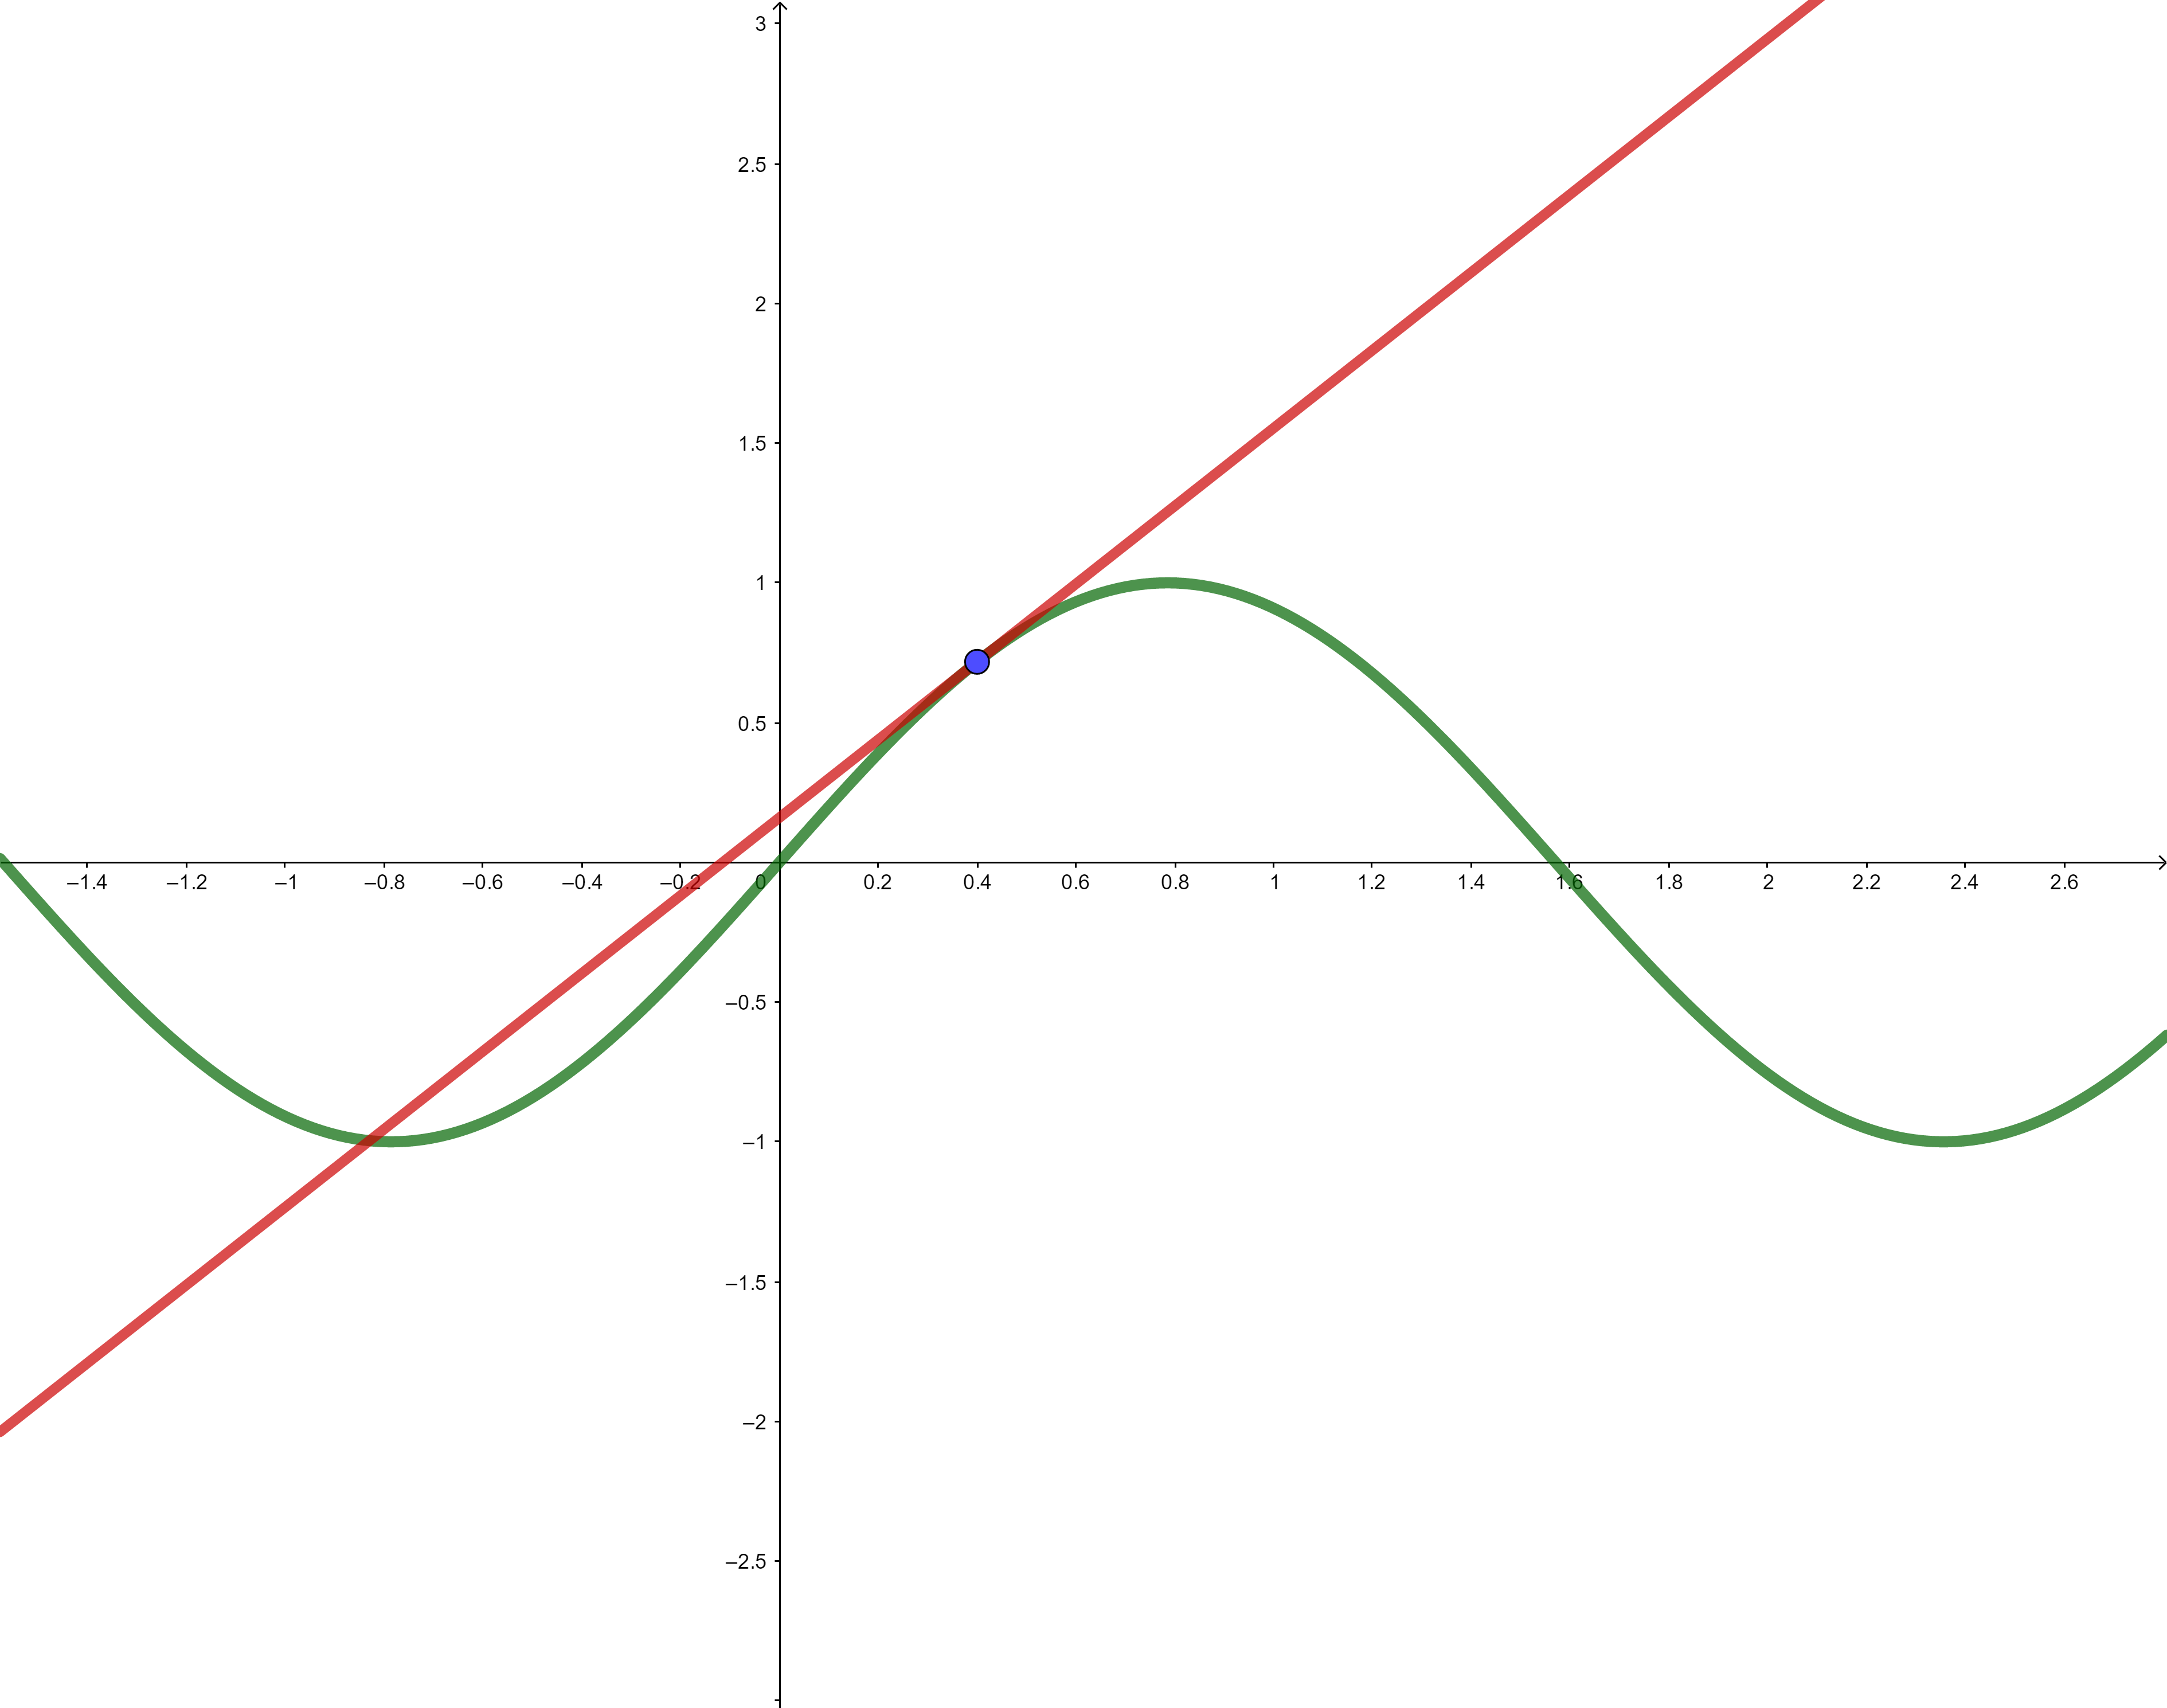
\includegraphics[width=\textwidth]{../Mathematik_2/Bilder/taylor_sinus_tangente.png}
%\end{minipage}
%	\begin{minipage}{0.6\textwidth}
%		F�r $\sin:x\mapsto \sin(x)$ lautet die Tangente in $x_0=2/5$: \[p_1:x\mapsto \sin(2/5) + \cos(2/5)(x-2/5)\]
%		Die Tangente erf�llt:
%	\begin{itemize}
%		\item $p_1(2/5) = \sin(2/5)$ ,
%		\item $p_1'(2/5) = \cos(2/5)$.
%	\end{itemize}
%\end{minipage}
%\end{exabox}
%
%F�r eine beliebige differenzierbare Funktion lautet die Tangentengerade an der Stelle $x_0$ also
%\[
%	p_1(x) =  f(x_0) + f'(x_0)(x-x_0)\,,
%\]
%und es gilt
%\begin{itemize}
%	\item $p_1$ l�uft durch den Punkt $(x_0|f(x_0))$, also $p_1(x_0) = f(x_0)$,
%	\item $p_1$ hat in $x_0$ dieselbe Steigung wie $f$, also $p_1'(x_0) = f'(x_0)$.
%\end{itemize}
%
%Als n�chstes kann man die quadratische Parabel suchen, die sich einer zweimal differenzierbaren Funktion $f$ an einer Stelle $x_0$ am besten ann�hert\footnote{im Sinne einer Interpolation.}: das ist die quadratische N�herung oder auch Schmiegeparabel.
%\begin{exabox}{Schmiegeparabel}{ }
%	\hspace{-0.3cm}\begin{minipage}{0.4\textwidth}
%		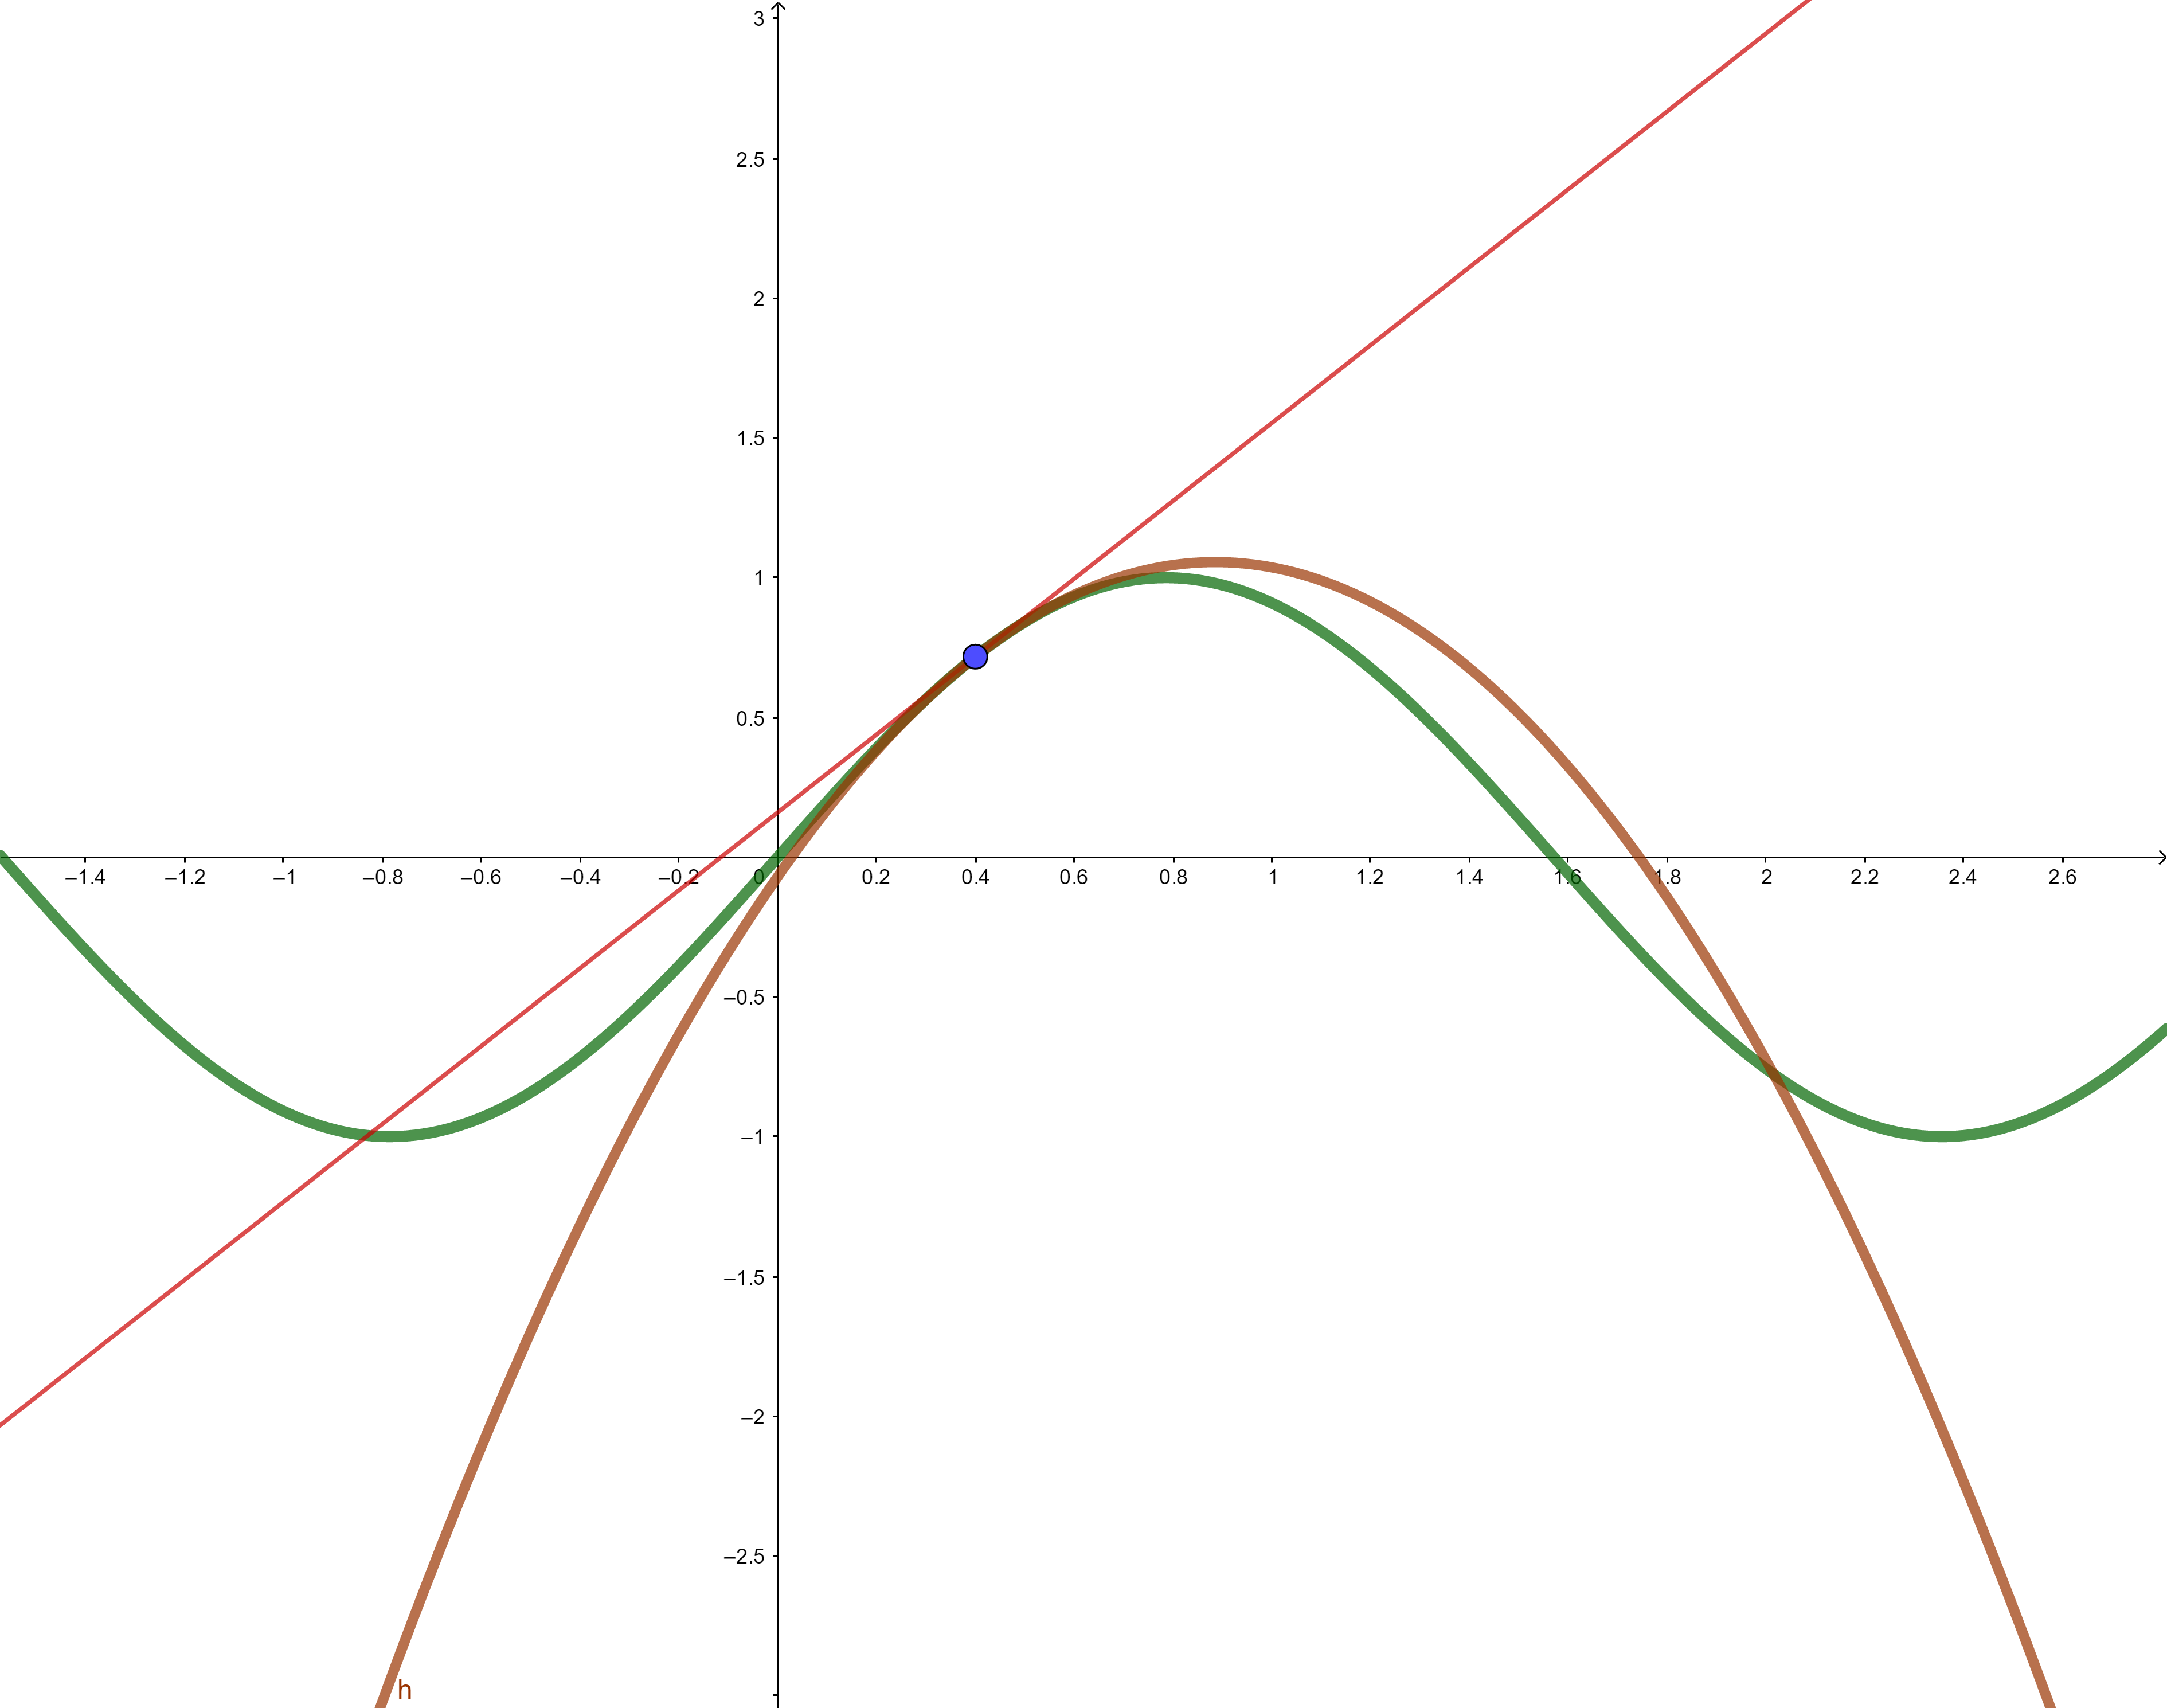
\includegraphics[width=\textwidth]{../Mathematik_2/Bilder/taylor_sinus_schmiegeparabel.png}
%\end{minipage}
%	\begin{minipage}{0.6\textwidth}
%		F�r $\sin:x\mapsto \sin(x)$ lautet die Schmiegeparabel in $x_0=2/5$: \[p_2:x\mapsto \sin(2/5) + \cos(2/5)(x-2/5) - 1/2\sin(2/5)(x-2/5)^2\]
%		Die Schmiegeparabel erf�llt:
%	\begin{itemize}
%		\item $p_2(2/5) = \sin(2/5)$ ,
%		\item $p_2'(2/5) = \cos(2/5)$.
%		\item $p_2''(2/5) = -\sin(2/5)$.
%	\end{itemize}
%\end{minipage}
%\end{exabox}
%
%F�r eine beliebige zweimal differenzierbare Funktion lautet die Schmiegeparabel an der Stelle $x_0$:
%\begin{eqnarray*}
%	p_2(x) &=&  f(x_0)+ f'(x_0)(x-x_0) +\frac12 f''(x_0)(x-x_0)^2,
%\end{eqnarray*}
%und es gilt
%\begin{itemize}
%	\item $p_2$ l�uft durch den Punkt $(x_0|f(x_0))$, also $p_2(x_0) = f(x_0)$,
%	\item $p_2$ hat in $x_0$ dieselbe Steigung wie $f$, also $p_2'(x_0) = f'(x_0)$.
%	\item $p_2$ hat $x_0$ dieselbe Kr�mmung wie $f$, also $p_2''(x_0) = f''(x_0)$.
%\end{itemize}
%
%Entsprechend  findet  man  die  Formeln  f�r  die beste lokale N�herung durch \underline{Polynome}\randverweis{MA1-polynome} dritten \ldots oder zehnten Grades:
%\begin{eqnarray*}
%	p_3(x) &=& f(x_0) + f'(x_0)(x-x_0)+ \frac12 f''(x_0)(x-x_0)^2+\frac16 f'''(x_0)(x-x_0)^3\,,\\
%	\cdots&&\\
%	p_{10}(x) &=& f(x_0) + f'(x_0)(x-x_0)+ \frac12 f''(x_0)(x-x_0)^2+ \cdots + \frac{1}{10!} f^{(10)}(x_0)(x-x_0)^{10}\,.
%\end{eqnarray*}
%
%\begin{exabox}{Taylor-Polynom vom Grad $10$}{ }
%	\begin{center}
%	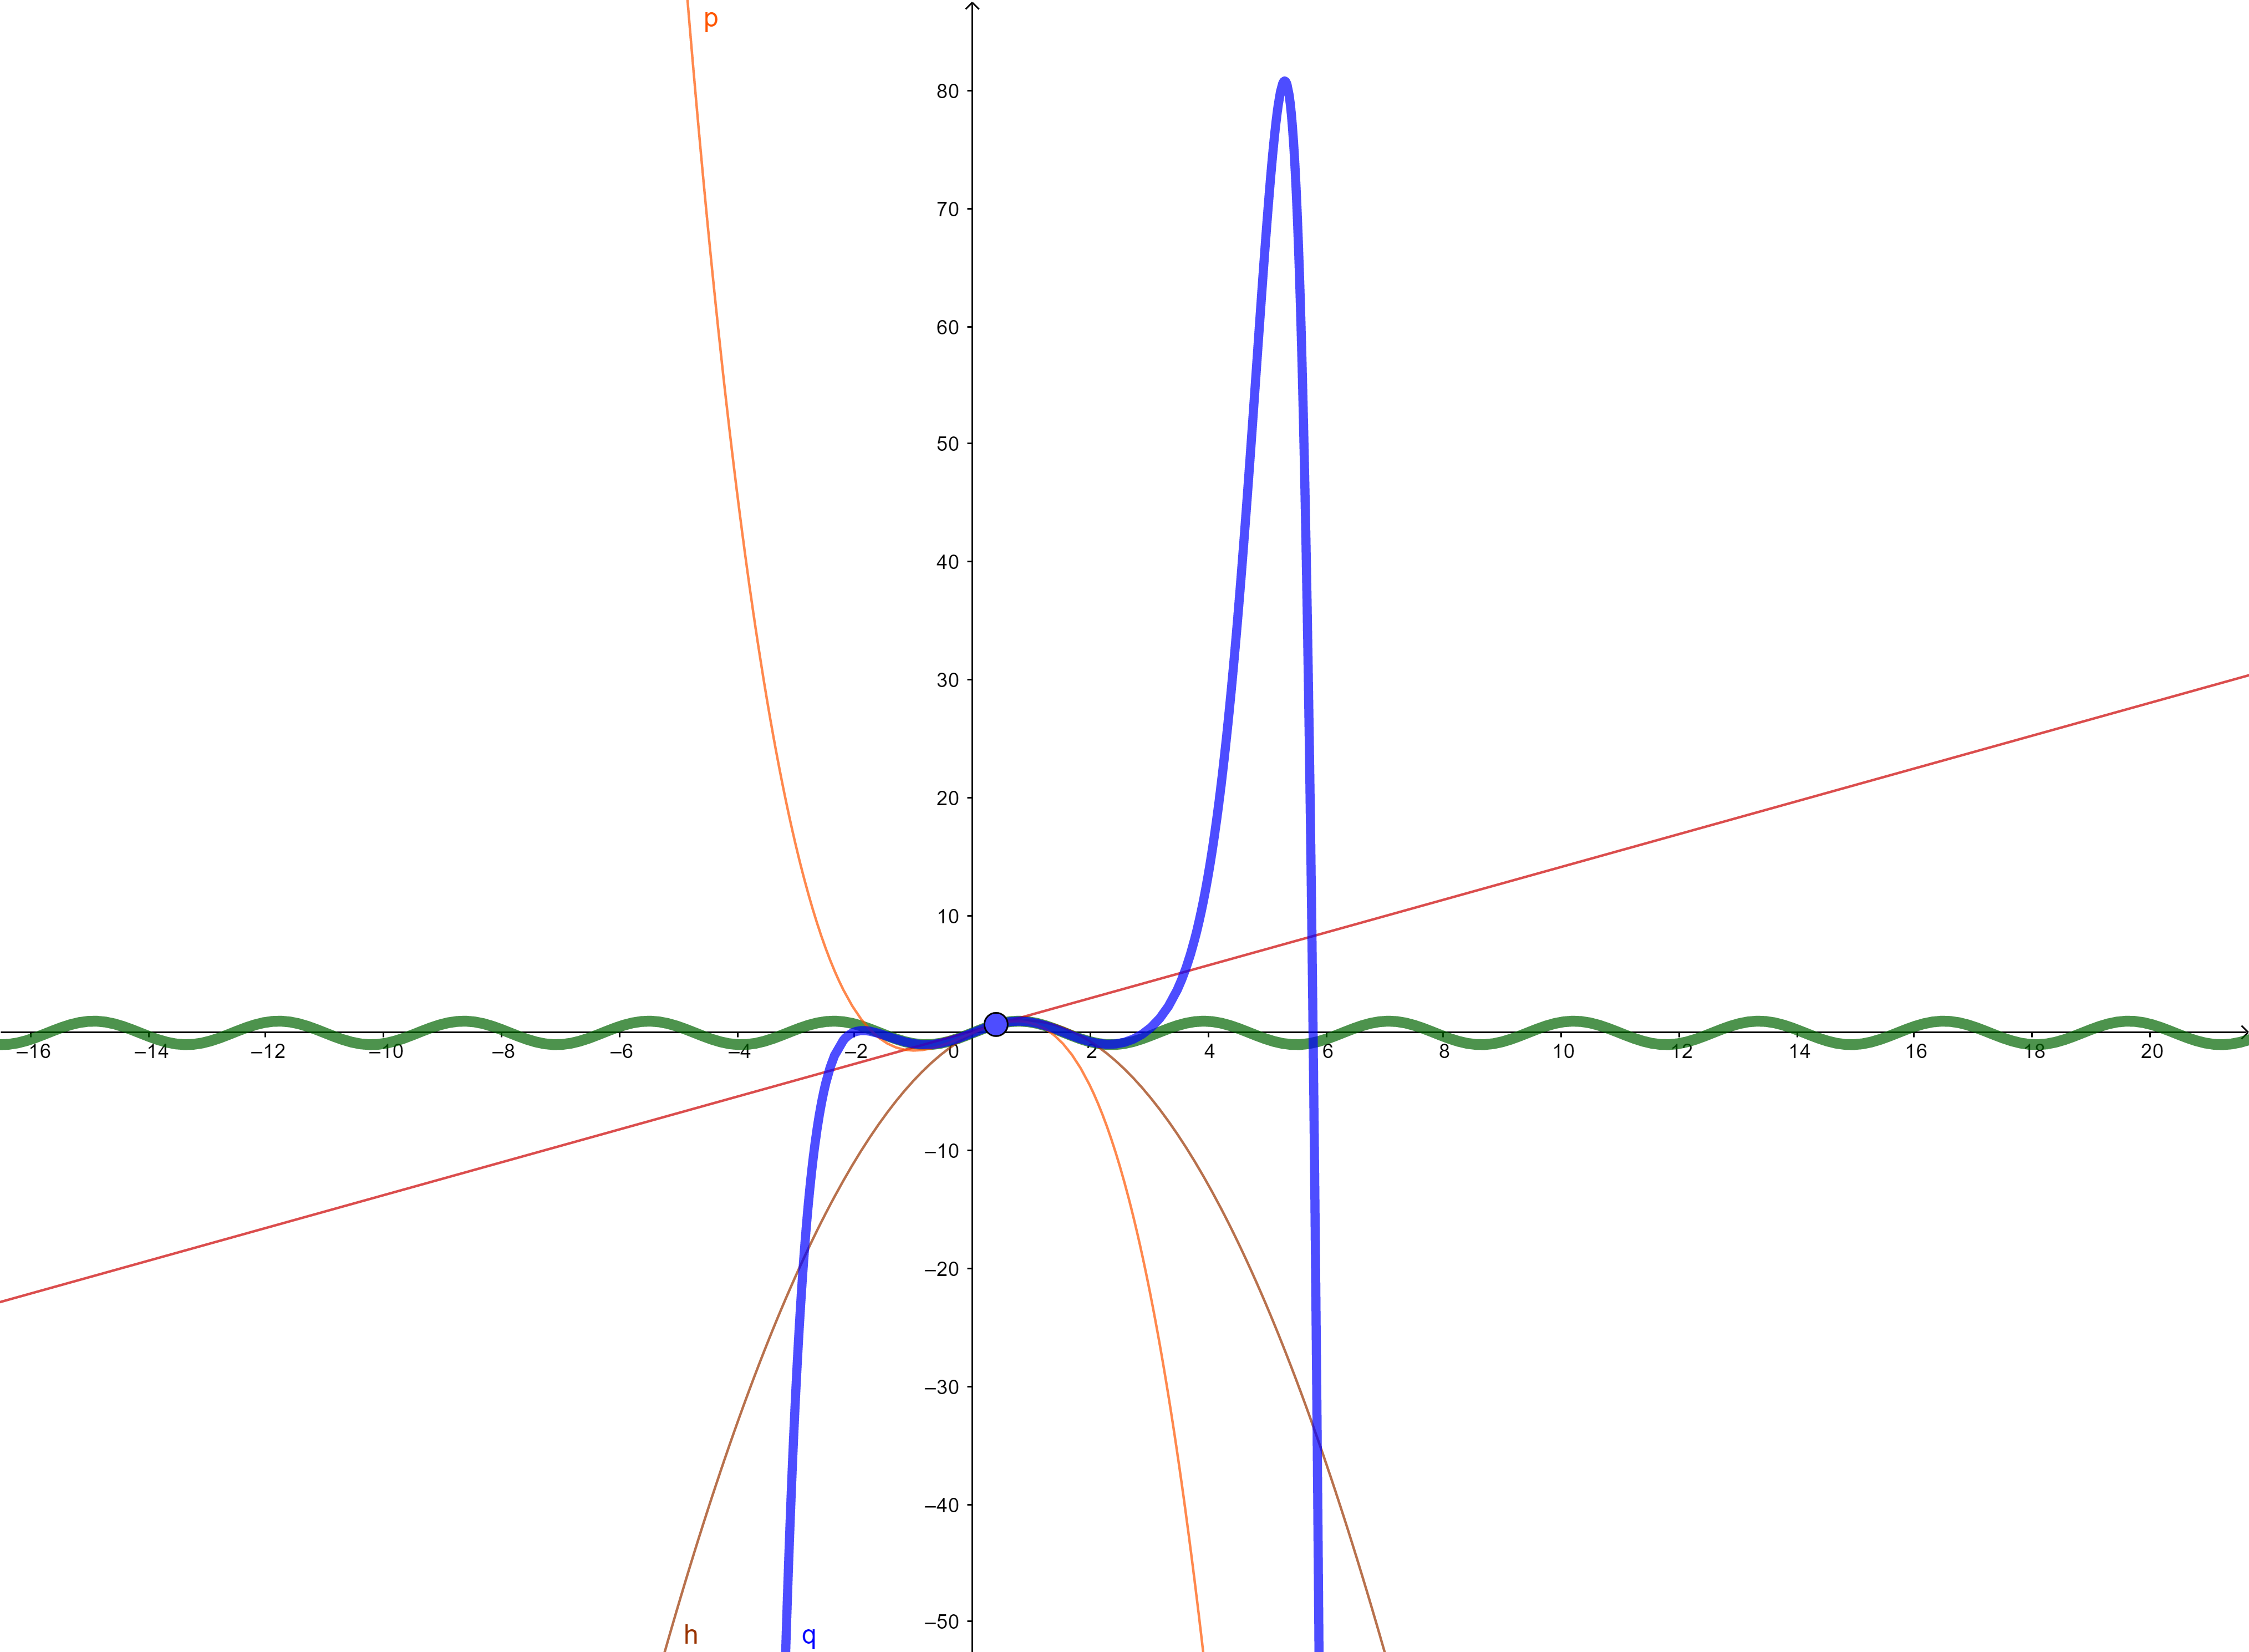
\includegraphics[width=0.7\textwidth]{../Mathematik_2/Bilder/taylor_sinus_polynom_grad_10.png}
%\end{center}
%\end{exabox}
%Vorausgesetzt die Funktion $f$ besitzt mindestens Ableitungen bis zur Ordnung $n$, dann kann man auf diese Weise ein Polynom $p_n$ vom Grad $n$ entwickeln, das sogenannte Taylor-Polynom vom Grad $n$:
%\begin{defbox}{Taylor-Polynom vom Grad $n$}{ }
%	F�r eine $n$-mal differenzierbare Funktion lautet das Taylor-Polynom vom Grad $n$:
%
%	\begin{eqnarray*}
%		p_n(x) &=& f(x_0) + f'(x_0)(x-x_0) + \frac12 f''(x_0)(x-x_0)^2 + \cdots + \frac{1}{n!} f^{(n)}(x_0)(x-x_0)^n \\
%		&=& \sum\limits_{k=0}^{n}\frac{1}{k!}f^{(k)}(x_0)(x-x_0)^k\,.
%\end{eqnarray*}
%Das Taylorpolynom $p_n$ stimmt an der Stelle $x=x_0$ mit der Funktion $f$ und mit deren Ableitung bis zum Grad $n$ �berein:
%\[ \forall\, k=0,\cdots,n: \quad p_n^{(k)}(x_0)= f^{(k)}(x_0)\,.  \]
%\end{defbox}
%
%\noindent Bemerkungen:\marginpar{\small Aufgaben}
%\begin{itemize}
%	\item In der Praxis ist nur das lokale Verhalten einer Funktion oder Kennlinie interessant. Um die Analyse zu erleichtern kann man anstatt der Orginalfunktion ein Taylorpolynom betrachten!
%	\item Das \underline{asymptotische Verhalten}\wennreferenzvorhanden{MA1-ableitungen-und-funktionsverlauf}{\marginpar{\small \ifintegriereaufgaben \abschnittsverweis{MA1-ableitungen-und-funktionsverlauf} \else \href{MA1-ableitungen-und-funktionsverlauf.pdf}{MA1-ableitungen-und-funktionsverlauf} \fi}} des Taylorpoynoms entspricht dem des Polynoms und kann unter Umst�nden ganz anders sein als das der betrachteten Funktion!
%	\item Wechselt man den Entwicklungspunkt $x_0$, muss man das Taylorpolynom neu bestimmen.
%\end{itemize}
%
%Im folgenden Beispiel wird die Wurzelfunktion an der Stelle $x_0 = 4$ mit einem Taylorpolynom vom Grad $3$ angen�hrt:
%\begin{exabox}{Taylor-Polynom an $f:x\to\sqrt{x}$ vom Grad $n=3$ an $x_0=4$}{ }
%Bestimmung der Ableitungen bis zum Grad $3$:
%\begin{eqnarray*}
%		f(x) &=& \sqrt{x} = x^{1/2}\,,\\[1ex]
%		f'(x) &=& \frac12 x^{-1/2} = \frac12 \frac{1}{\sqrt{x}}\,,\\[1ex]
%		f''(x) &=& -\frac14 x^{-3/2} =- \frac14 \frac{1}{\sqrt{x}^3}\,,\\[1ex]
%		f'''(x) &=& \frac38 x^{-5/2} =- \frac38 \frac{1}{\sqrt{x}^5}\,.
%	\end{eqnarray*}
%
%L�sung $p_3$ mit $x_0=4$:
%	\[
%	p_3:\mathbb R \to \mathbb R, x\mapsto 2 + \frac14(x-4)- \frac{1}{32} \frac{1}{2} (x-4)^2 + \frac{3}{256} \frac{1}{6} (x-4)^3\,.
%\]
%\begin{center}
%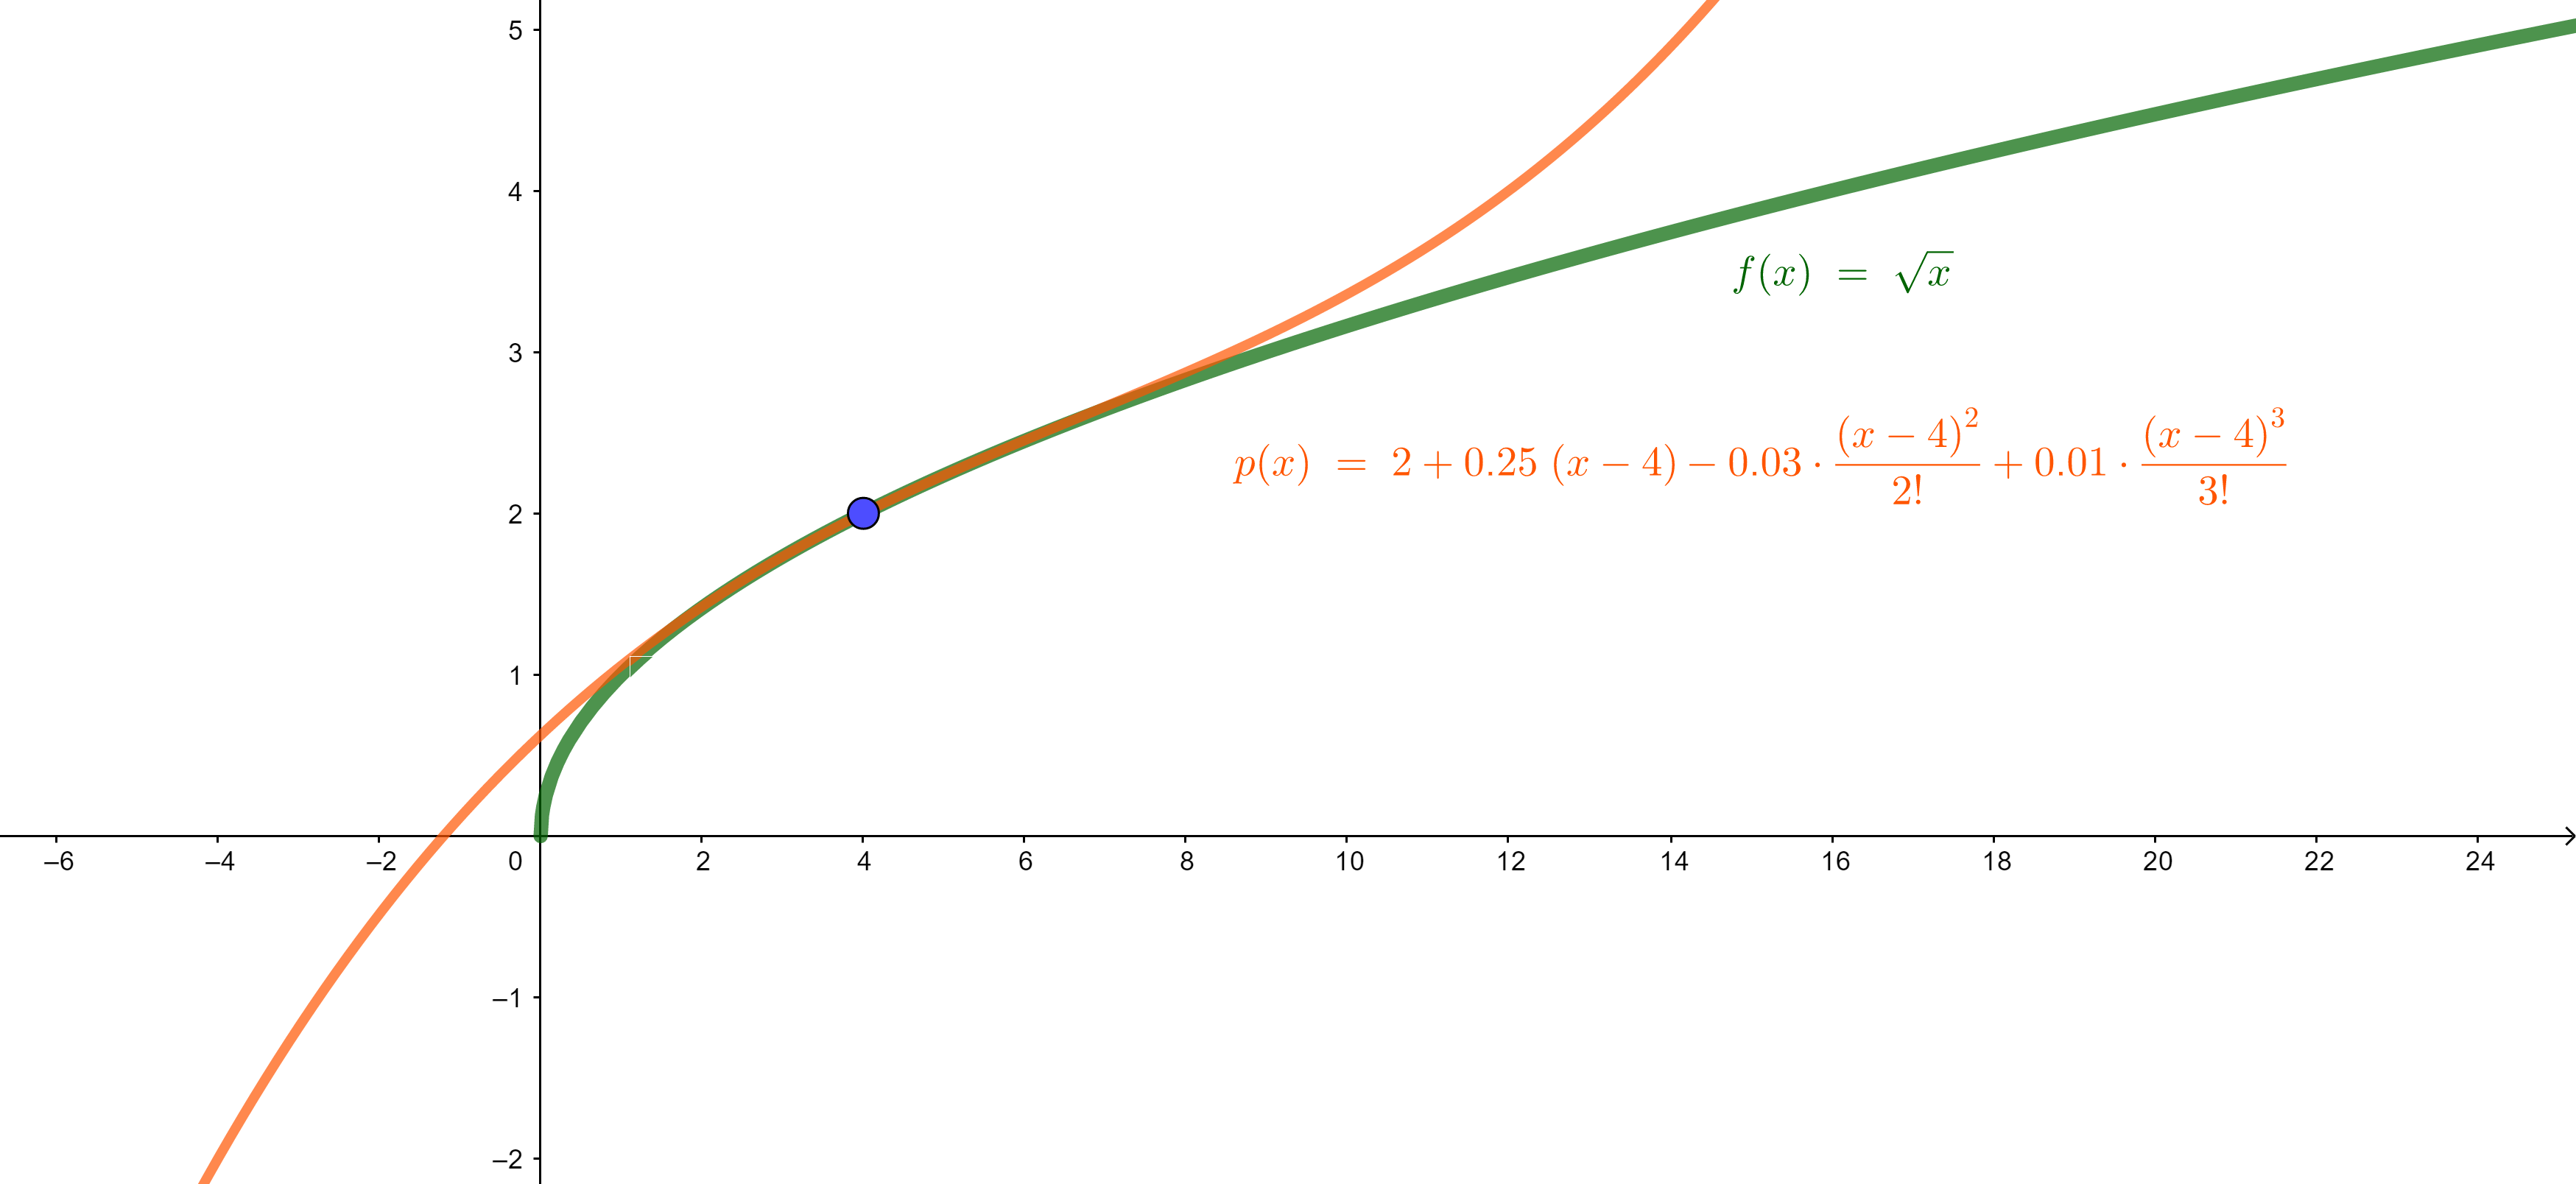
\includegraphics[width=0.7\textwidth]{../Mathematik_2/Bilder/taylor_wurzelfunktion_polynom_grad_3.png}
%\end{center}
%\end{exabox}
%%Auf diese Weise ist hier die Wurzelfunktion $f:x\mapsto \sqrt{x}$ mit einer im Vergleich zur Wurzelfunktion harmlosen kubischen Parabel gen�hert
%
%%Die N�herung ist offensichtlich nur in  der  Umgebung  der  Stelle  $x_0=4$  wirklich gut. Je weiter sich von der Entwicklungsstelle $x_0=4$ entfernt, desto gr��er wird der Fehler $|\sqrt{x} - p(x)|$. Es wird noch Thema in einem der folgenden Abschnitte sein diesen Fehler zu quantifizieren.
%%M�chte  man  die  Wurzelfunktion anderswo  n�hern,  braucht  man  eine andere  Parabel.  Au�erdem  sieht  man, dass die N�herung hier wirklich nur unter dem Mikroskop gilt: Wenn man sich nennenswert von dem Entwicklungspunkt  $4$  entfernt,  wird  die  N�herung  extrem  schlecht.  Demo  mit Wolfram Alpha: \begin{verbatim}series sqrt(x) at x=4 order 3 \end{verbatim}
%
%\subsection{Taylor-Reihe}
%
%F�r eine unendlich oft differenzierbare Funktion, kann man die N�herung durch Polynome immer weiter verbessern\footnote{im Sinne einer lokalen Approximation!} und gelangt damit formal zur Taylor-Reihe [Taylor series]:
%\begin{defbox}{Taylor-Reihe}{}
%	Eine unendlich oft differenzierbare Funktion l��t sich formal an jedem Punkt $x_0 \in D_f$ in eine Taylor-Reihe entwickeln:
%	\[
%	Tf(x,x_0): =  f(x_0) + f'(x_0)(x-x_0) + \cdots + \frac{f^{(n)}(x_0)}{n!}(x-x_0)^n + \cdots = \sum\limits_{k=0}^\infty \frac{f^{(k)}(x_0)}{k!}(x-x_0)^k \,.\]
%\end{defbox}
%
%\noindent Bemerkungen:
%\begin{itemize}
%	\item Die Struktur einer Taylor-Reihe ist anders als diejenige der unendlichen Reihen, die wir im vorangegangenen Kapitel\wennreferenzvorhanden{MA2-zahlenreihen}{\marginpar{\small \ifintegriereaufgaben \abschnittsverweis{MA2-zahlenreihen} \else \href{MA2-zahlenreihen.pdf}{MA2-zahlenreihen} \fi}} kennengelernt haben.
%	\item Anstatt Zahlen aufzuaddieren, werden hier Potenzen von $x$, also Funktionen, aufaddiert!
%	\item Fixiert man ein $x\in D_f$, und setzt es in die Reihe ein, dann erh�lt man eine unendliche Reihe nach dem Schema des letzten Abschnitts. Beispielsweise f�r $x=3, x_0=0$:
%		\[
%	\sum\limits_{k=0}^\infty \frac{f^{(k)}(0)}{k!}3^k = \sum\limits_{k=0}^\infty a_k, \quad a_k := \frac{f^{(k)}(0)}{k!}3^k \in \mathbb R  \,.
%\]
%\item Eine unendliche Reihe, in der Potenzen von $x$ aufsummiert werden - garniert mit einem Koeffizienten - bezeichnet man Potenzreihen
%	\[
%		\sum\limits_{k=0}^\infty c_k x^k \,.
%	\]
%	Taylor-Reihen sind also spezielle Potenzreihen.
%	\end{itemize}
%
%Zwei Fragen stellen sich:
%\begin{itemize}
%	\item Gibt es $x \in D_f$, f�r die die Taylor-Reihe \underline{konvergieren}\randverweis{MA2-zahlenreihen}?
%	\item Wenn wir ein $x \in D_f$ identifiziert haben, f�r das die Taylor-Reihe konvergiert, gilt dann Gleichheit, also: $\forall \, x\in D_f:\quad Tf(x,x_0) = f(x)$?
%\end{itemize}
%Klar ist: falls wir Bedingungen kennen, unter denen sich die Fragen mit ja beantworten lassen, dann bedeutet das einen enormen Gewinn, denn $f$, egal wie kompliziert, wird pl�tzlich einfach berechenbar. Es lohnt sich also auf diese Fragen einzugehen und das werden wir in den n�chsten Abschnitten tun. F�r den Moment konzentrieren wir uns noch auf das Erlernen des Handwerkszeugs: wir entwickeln Taylor-Reihen!
%
%\begin{exabox}{Taylor-Reihe f�r $f: x\mapsto \exp(x)$ }{ }
%	Funktion: \[ f: \mathbb R \to (0,\infty),  x\mapsto e^x \]
%	Entwicklungspunkt:
%	\[ x_0 \in \mathbb R : \; x_0 = 0\,.\]
%	Ableitungen:
%\[
%	\forall\, k\in \mathbb N_0:\quad f^{(k)}(x) = e^x \Rightarrow  	f^{(k)}(0) = 1\,.
%\]
%	Taylor-Reihe mit $x_0=0$:
%	\[
%	Tf(x,0):= x + \cdots + \frac{1}{n!}x^n + \cdots = \sum\limits_{k=0}^\infty \frac{1}{k!}x^k \,.
%\]
%\end{exabox}
%
%\begin{exabox}{Taylor-Reihe f�r $f: x\mapsto \exp(ix)$ }{ }
%	Funktion: \[ f: \mathbb R \to \mathbb C, x \mapsto e^{ix} \]
%	Entwicklungspunkt:
%	\[ x_0 \in \mathbb R :\; x_0 = 0\,.\]
%	Ableitungen\dots
%\[
%	\forall\, k\in \mathbb N_0:\quad f^{(k)}(i x) = i^k e^{i x} \Rightarrow  	f^{(k)}(0) = i^k\,.
%\]
%	Taylor-Reihe mit $x_0=0$:
%\[ Tf(x,0):=1 + \cdots + \frac{i^n}{n!}x^n + \cdots = \sum\limits_{k=0}^\infty \frac{i^k}{k!}x^k \,.\]
%\end{exabox}
%
%\noindent Bemerkungen:\marginpar{\small Aufgaben}
%\begin{itemize}
%	\item Um eine N�herung beispielsweise an die Zahl $e^{1/2}$ anzugeben, summeriert man die ersten f�nf bis zehn Summanden dieser Reihe auf.
%	\item Entsprechend betrachtet man eine Talyor-Reihe f�r ein komplexes Argument $z=x+iy$ und kann eine N�herung von $e^{3+4i}$ angeben.
%\end{itemize}
%
%Die \underline{Eulersche Identit�t}\randverweis{MA1-komplexe-zahlen-polarform-und-euler}
%\[
%	re^{i\varphi} = r ( \cos(\varphi) + i\sin(\varphi) )\,.
%\]
%er�ffnet einen Weg, um von der komplexen Exponentialfunktion zu den \underline{trigonometrischen Funktionen}\randverweis{MA1-trigonometrische-funktionen} zu gelangen. Die Taylor-Reihen f�r Sinus und Kosinus sind folgende Potenzreihen:
%\begin{exabox}{Taylor-Reihe f�r $f_1:x\mapsto \sin(x)$ und $f_2:x\mapsto \cos(x)$}{ }
%	Funktionen:
%	\[\begin{cases}
%			f_1: &\mathbb R \to \mathbb R, x\mapsto \sin(x) \\
%			f_2: &\mathbb R \to \mathbb R, x\mapsto \cos(x) \\
%		\end{cases}
%	\]
%	Ableitungen:
%	\begin{center}
%		\begin{tabular}{c|c c c c c c c c c c }
%			& $f(0)$ & $f{(1)}(0)$ & $f^{(2)}(0)$ & $f^{(3)}(0)$ &$f^{(4)}(0)$ & $f^{(5)}(0)$ & $f^{(6)}(0)$ & $f^{(7)}(0)$ &  \ldots \\
%			\hline
%			$\sin$ & $0$ & $1$ & $0$ &  $-1$ & $0$ & $1$ & $0$ &  $-1$ &\ldots \\
%			$\cos$ & $1$ & $0$ & $-1$&  $0$ & $1$ & $0$ & $-1$&  $0$ &\ldots
%		\end{tabular}
%	\end{center}
%	Taylor-Reihen mit $x_0=0$:
%	\begin{eqnarray*}
%		\begin{cases}
%			Tf_1(x,0)=  x - \displaystyle{\frac{1}{3!}} x^3 + \displaystyle{\frac{1}{5!}} x^5 -+  \cdots = \displaystyle{\sum\limits_{k=0}^\infty} (-1)^{k} \displaystyle{\frac{1}{(2k+1)!}} x^{2k+1} \,,\\[1ex]
%			Tf_2(x,0) =  1 - \displaystyle{\frac12} x^2 + \displaystyle{\frac{1}{4!}} x^4 - \displaystyle{\frac{1}{6!}} x^6 +-  \cdots = \displaystyle{\sum\limits_{k=0}^\infty} (-1)^{k}\displaystyle{\frac{1}{(2k)!}} x^{2k} \,.
%		\end{cases}
%	\end{eqnarray*}
%%Betrachtet man nur die ersten $n$ Summanden, erh�lt man Taylor-Polynome, die sich mehr und mehr um die $x$-Achse wickeln, um sich dann entsprechen $x^n$ asymptotisch Unendlich ann�hern:
%	\centering
%	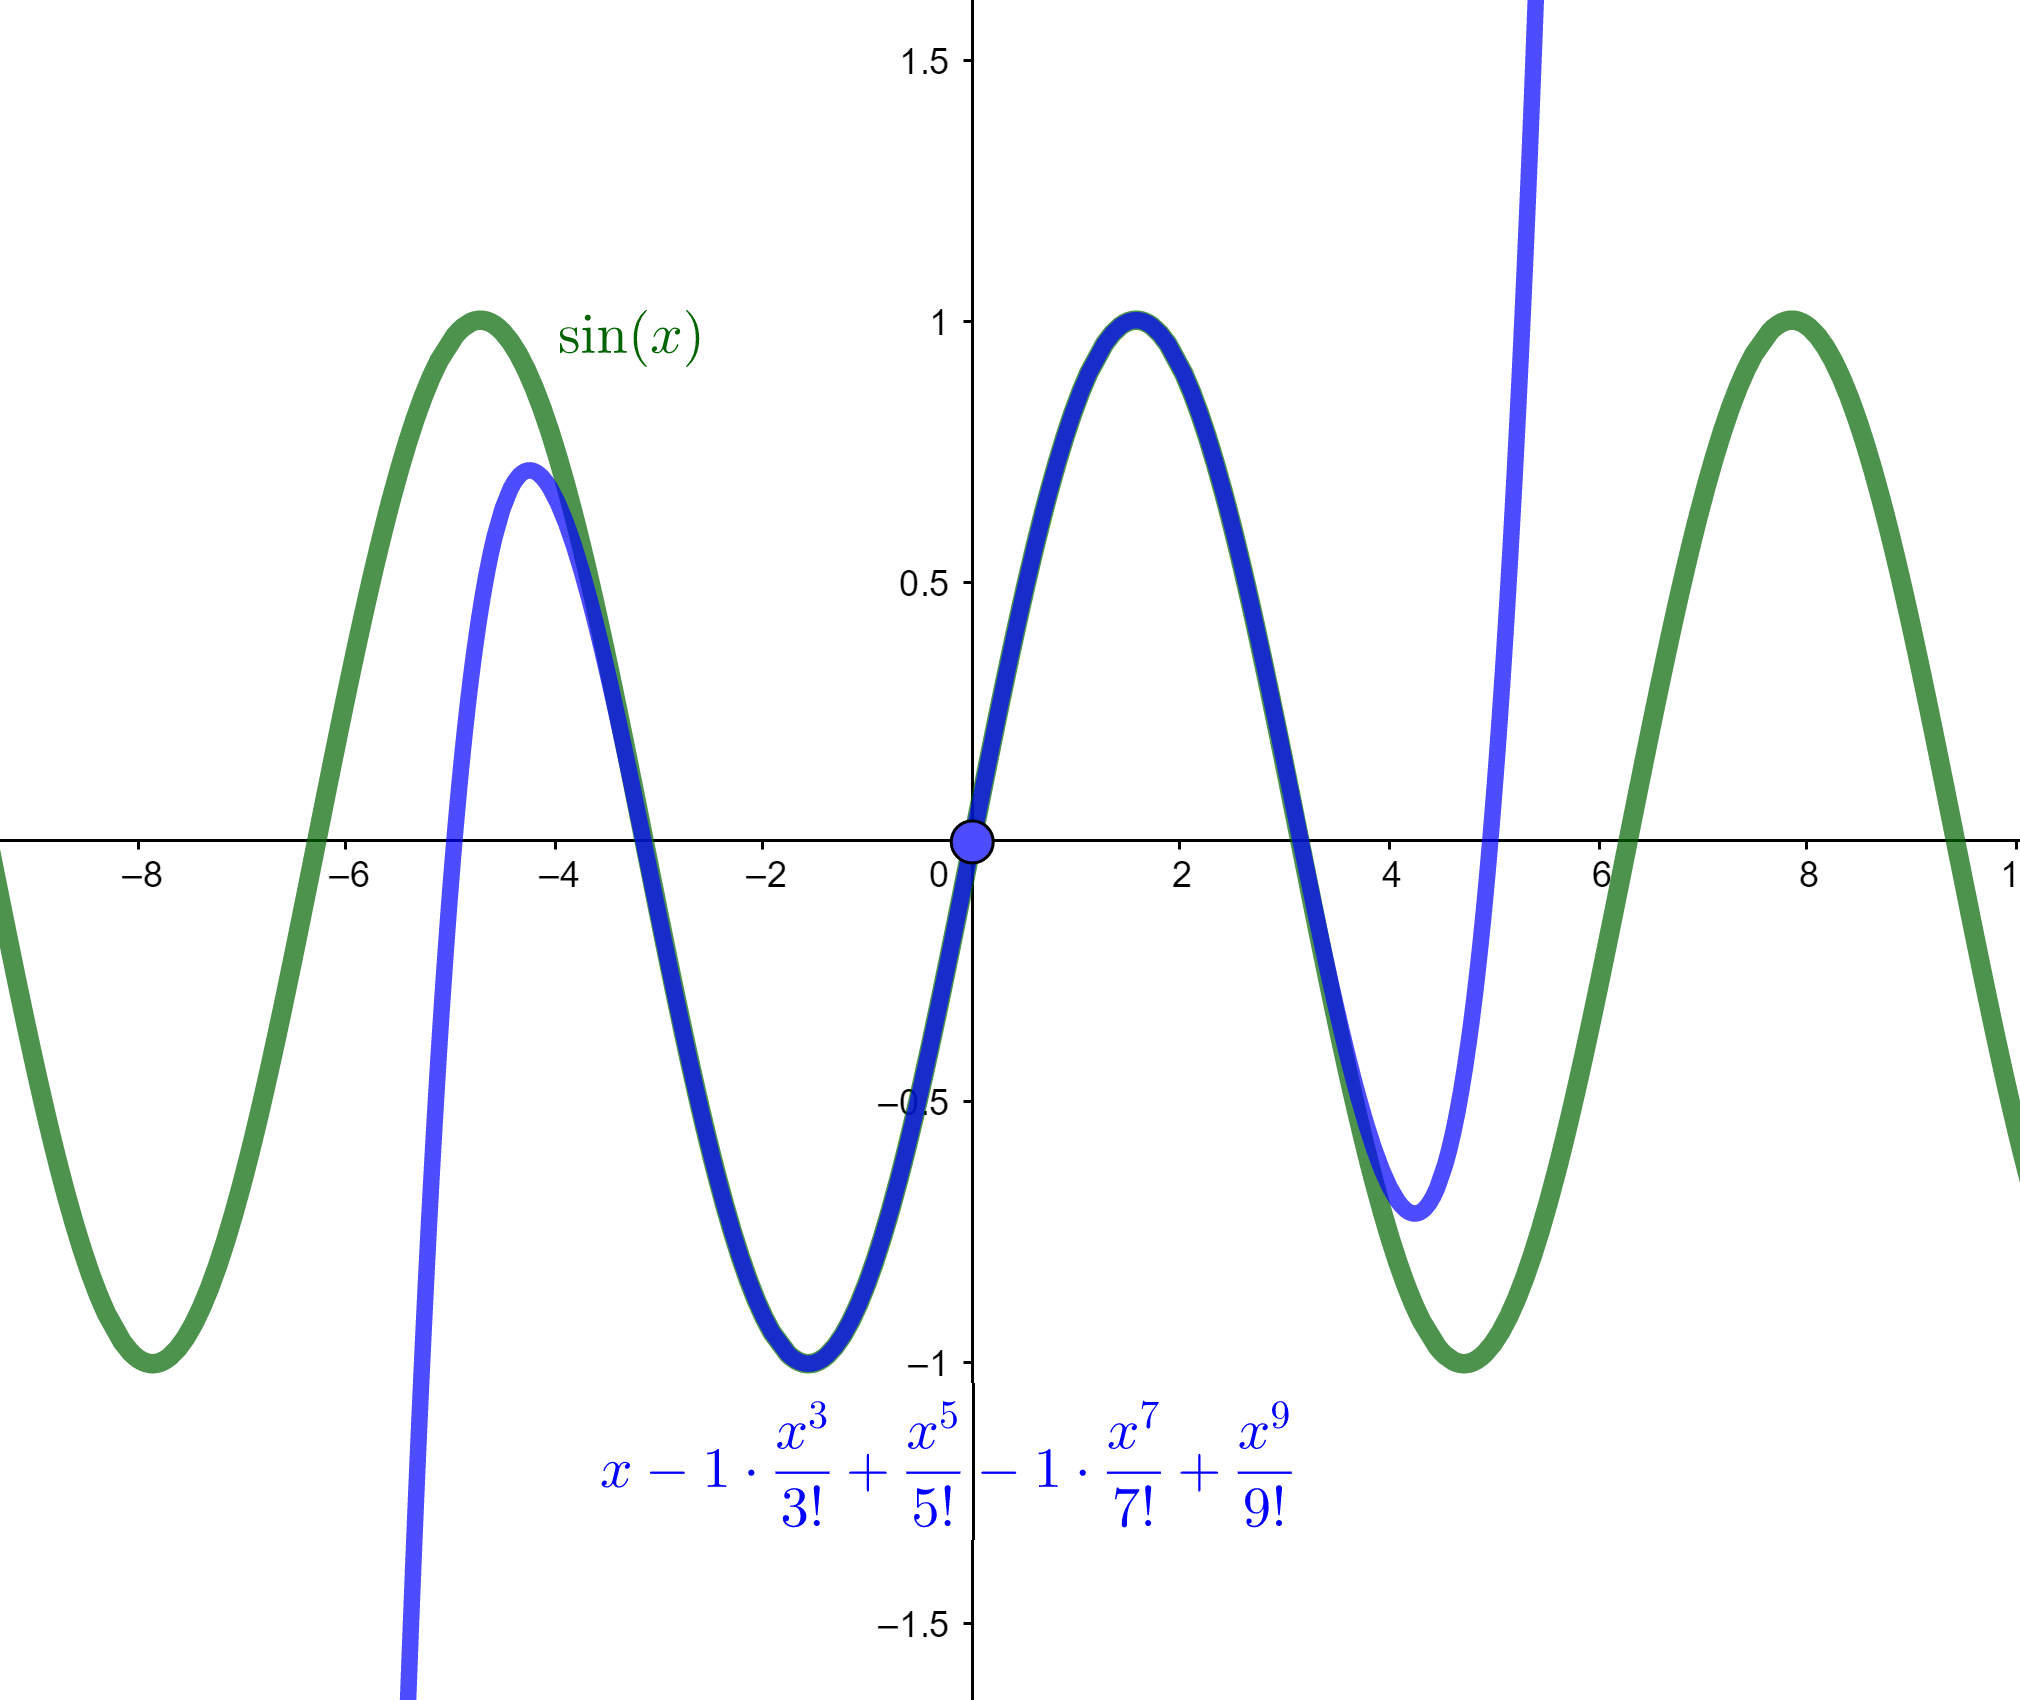
\includegraphics[width=0.6\textwidth]{../Mathematik_2/Bilder/taylor_sinus_maclaurinpolynom_grad_10.png}
%\end{exabox}
%%Demo mit Wolfram Alpha: \begin{verbatim} series sin(x) at x=0 order 20 \end{verbatim} Durch Einsetzen von $x=i \varphi$ in die Potenzreihe f�r die Exponentialfunktion findet man:
%
%Als n�chstes Beispiel entwickeln wir die \underline{gebrochenrationale Funktion}\randverweis{MA1-rationale-funktionen} $f: x\mapsto 1/(1-x)$ an der Stelle $x_0=0$.
%
%Dazu sind die Ableitungen dieser Funktion zu bestimmen und an der Stelle \(x_0=0\) auszuwerten:
%\begin{exabox}{Taylor-Reihe f�r $f:x\mapsto 1/(1-x)$}{ }
%	Funktion: \[ f: \mathbb R\setminus\{ 1\} \to \mathbb R, x \mapsto \frac{1}{1-x} \]
%	Ableitungen:
%	\begin{center}
%		\begin{tabular}{cccccc}
%			$f(x)$ & $f^{(1)}(x)$ & $f^{(2)}(x)$ & $f^{(3)}(x)$ &  \ldots & $f^{(n)}(x)$\\
%			\hline
%			$(1-x)^{-1}$ & $(1-x)^{-2}$ & $2(1-x)^{-3}$ & $6(1-x)^{-4}$ & \ldots & $n!(1-x)^{-n-1}$
%		\end{tabular}
%	\end{center}
%	Taylor-Reihe mit $x_0=0$:
%	\begin{eqnarray*}
%		Tf(x,0) = \frac{1}{1-x} =  1 +x + 2\frac{1}{2!} x^2 + 3!\frac{1}{3!} x^3 \cdots  + n!\frac{1}{n!} x^n + \cdots = \sum\limits_{k=0}^\infty x^{k} \,. \quad(**)
%	\end{eqnarray*}
%\end{exabox}
%
%\noindent Bemerkungen:
%\begin{itemize}
%	\item Benutzt man die Tayplor-Reihen zur Darstellung von $\sin$ und $\cos$, so ist  $x$  im Bogenma� einzusetzen, denn die Ableitungen von Sinus und Cosinus bildet man typischerweise im Bogenma�!
%	\item Die Taylor-Reihen, die wir f�r die Exponentialfunktion entwickelt haben, kennen wir schon und wir wissen auch schon, dass die Taylor-Reihe die Exponentialfunktion f�r jedes $x\in \mathbb K$ mit $\mathbb K = \mathbb R$ oder $\mathbb C$ darstellt! Das Thema Konvergenz scheint hier kein Problem zu sein.
%	\item Bei $(**)$ sieht das anders aus, wie folgendes Experiment zeigt: multiplizieren wir die Partialsumme $1+x+x^2+x^3+\dots + x^n$ mit $(1-x)$, dann erhalten wir \marginpar{\small Aufgabe}:
%\begin{eqnarray*}
%\left( 1 + x + x^2 + \cdots + x^n\right) \cdot (\textcolor{blue}{1}\textcolor{brown}{-x}) &=& \textcolor{blue}{ 1+ x + x^2 + \cdots + x^n}\textcolor{brown}{  -  x - x^2 - x^3 - \cdots - x^{n+1}} \\
%&=& \textcolor{blue}{1} \textcolor{brown}{- x^{n+1} }\\[1ex]
% \stackrel{\displaystyle{x\not=1}}{\Rightarrow}  && 1+x+x^2 + \cdots + x^n = \frac{1-x^{n+1}}{1-x} \,.
%\end{eqnarray*}
% %eine Teleskopsumme [telescope sum}
%
%Der Term auf der rechten Seite des letzten Gleichheitszeichen entspricht also f�r $n\to \infty$ der Taylor-Reihe $(**)$.
%\[
%	\lim\limits_{n\to\infty} \left( 1 + x + x^2 + x^3 + \cdots + x^n\right) = \lim\limits_{n\to\infty} \frac{1-x^{n+1}}{1-x} = \textnormal{?}
%\]
%Die Konvergenz der Reihe muss also ma�geblich von dem Wertebereich von $x$ abh�ngen, denn
%\begin{eqnarray*}
%	\big|x^{n+1}\big|  \to \begin{cases}  \infty, \quad &|x| > 1 \,, \\
%		1, \quad& |x| = 1\,,\\
%		0, \quad &|x| < 1\,.
%	\end{cases}
%\end{eqnarray*}
%Also k�nnen wir an der Stelle schlie�en:
%\[
%	\lim\limits_{n\to\infty} \left( 1 + x + x^2 + x^3 + \cdots + x^n\right) = \frac{1}{1-x} \quad \textnormal{falls}\quad -1 < x < 1\,.
%\]
%\end{itemize}
%
%\subsection{Taylor-Restformel}
%
%Eine Funktion $f$ soll an der Stelle $x_0$ mit einem Taylor-Polynom $n$-ten Grades gen�hert werden, also durch den Anfang der Taylor-Reihe:
%\[
%	f(x) \approx p_n(x) = f(x_0) + f'(x_0)(x-x_0) + \frac{1}{2!}f''(x_0)(x-x_0)^2 + \cdots +  \frac{1}{n!}f^{(n)}(x_0)(x-x_0)^n\,.
%\]
%
%Die Frage ist, wie gut diese N�herung an einer Stelle $x$ ist. Anschaulich scheint es so, dass die N�herung lokal um so besser ist, je n�her $x$ an $x_0$ ist und je h�her der Grad $n$ ist. Um das zu untersuchen, betrachtet man die Abweichung der Funktion $f$ von der N�herung. Der Fehler bzw. Rest $R_n$ ist:
%
%\[
%	R_n(x) = f(x) -p_n(x) = f(x) -\left(  f(x_0) + f'(x_0)(x-x_0) + \frac{1}{2!}f''(x_0)(x-x_0)^2 + \cdots +  \frac{1}{n!}f^{(n)}(x_0)(x-x_0)^n \right) \,.
%\]
%
%F�r $R_1$, also den Fehler der Tangentengerade \(\textcolor{blue}{p_1(x) = f(x_0) + f'(x_0)(x-x_0)}\), ergibt sich:
%\[
%	R_1(x) = f(x) - p_1(x)  = \int\limits_{x_0}^x f''(t)(x-t)\,\mathrm{d}t\,,
%\]
%denn mit partieller Integration folgt\randverweis{MA2-integrationsregeln}
%\begin{eqnarray*}
%	\int\limits_{x_0}^x f''(t)(x-t)\,\mathrm{d}t &=& \Big[ f'(t)(x-t)\Big]_{t = x_0}^{t=x} - \int\limits_{x_0}^x f'(t) (-1) \,\mathrm{d}t \\
%	&=& 0 \textcolor{blue}{- f'(x_0)(x-x_0)} + \left( f(x) \textcolor{blue}{-f(x_0)}\right) = f(x) \textcolor{blue}{-p_1(x)} = R_1(x)\,.
%\end{eqnarray*}
%
%F�r $R_2$, also der Fehler der Schmiegeparabel \(p_2(x) = f(x_0) + f'(x_0)(x-x_0) + \frac12 f''(x_0)(x-x_0)^2\), ergibt sich:
%\[
%	R_2(x) = f(x) - p_2(x)  = \frac12 \int\limits_{x_0}^x f'''(t)(x-t)^2\,\mathrm{d}t\,,
%\]
%Das zeigt man, indem man diesen Ausdruck mit Hilfe einer \underline{partiellen Integration}\randverweis{MA2-integrationsregeln} auf $R_1$ zur�ckf�hrt:
%\begin{eqnarray*}
%	\frac12\int\limits_{x_0}^x f'''(t)(x-t)^2\,\mathrm{d}t &=& \Big[ f''(t)(x-t)^2\Big]_{t = x_0}^{t=x} + \int\limits_{x_0}^x f''(t) (x-t) \,\mathrm{d}t \\
%	&=& 0 -\frac12 f''(x_0)(x-x_0)^2 + R_1(x) = f(x) \underbrace{- p_1(x) -\frac12 f''(x_0)(x-x_0)^2}_{\displaystyle{=- p_2(x)}} = R_2(x)\,.
%\end{eqnarray*}
%
%Nach diesem Muster ergibt sich offensichtlich allgemein f�r $R_n$, also den Fehler des Taylor-Polynoms $n$-ten Grades:\footnote{Man findet in der Literatur eine �quivalente Darstellung des Restglieds. Sie hei�t Restglied nach Lagrange: es existiert ein \(\xi\in (x_0,x)\) mit \( R_n(x) = \frac{1}{(n+1)!} f^{(n+1)}(\xi)(x-x_0)^{n+1}\,. \) }
%\begin{theorembox}{Taylor-Restformeln: Integrale Darstellung}{ }
%	Sei $D_f\subset \mathbb R$ ein Intervall und $f:D_f\to \mathbb R$ eine $(n+1)$-mal stetig differenzierbare Funktion. Schneidet man die Taylor-Reihe nach dem $n$-ten Glied an, so gilt
%\[
%	f(x) = p_n(x) + R_n(x),\quad \textnormal{mit}\; R_n(x) = \frac{1}{n!} \int\limits_{x_0}^x f^{(n+1)}(t)(x-t)^{n}\,\mathrm{d}t\,.
%\]
%\end{theorembox}
%
%\subsection{Absch�tzung des Fehlers}
%
%Die Formel f�r $R_n$ erlaubt  zu  sagen,  wie  dicht $x$ an $x_0$ liegen  muss  und wie hoch der Grad $n$ gew�hlt werden muss, um den Fehler $R_n$ hinreichend klein zu halten. Typischerweise gibt man dazu vor, wie gro� der Absolutbetrag des Fehlers maximal sein darf (sagen wir eine Zahl $F$). Also ist die Frage, f�r welche $x$ und f�r welche $n$ dies gilt:
%\[
%	| R_n(x)| = \Big| f(x) - p_n(x)\Big|  \leq F \,.
%\]
%
%Das Integral auszurechnen, ist mit Bleistift und Papier oft gar nicht m�glich. Man gibt sich mit einer konservativen Sch�tzung zufrieden, d. h. einer Sch�tzung, die auf der sicheren Seite liegt, den Fehler im Betrag also allenfalls zu gro� sch�tzt und nie zu klein. Das Integral �ndert man dazu so, dass es im Betrag allenfalls gr��er werden kann. Betrachten wir zun�chst den Fall $x>x_0$:
%\begin{eqnarray*}
%	| R_n(x)| = \Big|\frac{1}{n!} \int\limits_{x_0}^x f^{(n+1)}(t)(x-t)^{n}\,\mathrm{d}t \Big| &\leq& \frac{1}{n!} \int\limits_{x_0}^x \big| f^{(n+1)}(t)(x-t)^{n}\big|\,\mathrm{d}t  = \frac{1}{n!} \int\limits_{x_0}^x \big| f^{(n+1)}(t)\big|(x-t)^{n}\,\mathrm{d}t \\
%	&\leq&  \frac{\max\limits_{x_0 \leq \xi \leq x} \big| f^{(n+1)}(\xi)\big| }{n!} \int\limits_{x_0}^x (x-t)^{n}\,\mathrm{d}t \\
%		&\leq&  \max\limits_{x_0 \leq \xi \leq x} \big| f^{(n+1)}(\xi)\big|  \frac{1}{(n+1)!} (x-x_0)^{n+1}\,.
%	\end{eqnarray*}
%
%	\begin{theorembox}{Absch�tzung des Fehlers}{ }
%	Sei $D_f\subset \mathbb R$ ein Intervall und $f:D_f\to \mathbb R$ eine $(n+1)$-mal stetig differenzierbare Funktion. Es gilt:
%\begin{eqnarray*}
%	| R_n(x)| \leq  \max\limits_{\xi\in [x_0,x]} \big| f^{(n+1)}(\xi)\big|  \frac{1}{(n+1)!} |x-x_0|^{n+1}\,.
%	\end{eqnarray*}
%\end{theorembox}
%
%Wenn man $x$ und $n$ so w�hlt, dass dieser Ausdruck kleiner als die gew�nschte Fehlerschranke $F$ ist, dann ist es der Betrag $|R_n|$ des wahren Fehlers erst recht.
%
%Betrachten wir beispielsweise wieder die Wurzelfunktion $f: x\mapsto \sqrt{x}$.  Wie gro� ist der Fehler, wenn wir die $f$ an $x_0=4$ mit einer quadratischen Parabel $p_2$ ann�hern?
%\begin{exabox}{Fehlerabsch�tzung f�r $R_2(x)$ f�r $x_0=4$ im Intervall \( [1,7]\)}{ }
%	Taylor-Polynom $p_2$ f�r $x_0=4$:
%\[
%	p_2(x) = 2 + \frac{1}{2\sqrt{4}}(x-4) - \frac{1}{8\sqrt{4}^3}(x-4)^2 \,.
%\]
%Gr��tm�glicher Fehler im Intervall \( x\in [1,7]\):
%\[
%	\Big| R_2(x)\Big| \leq \underbrace{\max\Big| \frac38 \xi^{-5/2}\Big|}_{\leq 3/8 1^{-5/2}}  \cdot\underbrace{ \frac{(x-4)^3}{6}}_{\leq 3^3/6} \leq \frac{3}{8}\frac{3^3}{6} = \frac{27}{16}\,.
%\]
%\end{exabox}
%
 \newpage % 03 Taylorreihen % VPL Approximationfehler Matlab
%\setcounter{exercise}{0} \ifintegriereaufgaben
\section*{Taylorreihen Aufgaben}\label{MA2-taylorreihen-aufgaben}

 Erkl�rungen und Beispiele, die zur Bearbeitung der Aufgaben hilfreich sind, finden Sie im Skript\wennreferenzvorhanden{MA2-taylorreihen}{ (Abschnitt \abschnittsverweis{MA2-taylorreihen})} und, falls Sie nicht weiterkommen, dann schauen Sie \hyperref[MA2-taylorreihen-loesungen]{hier}.

\else
\section{Taylorreihen Aufgaben}\label{MA2-taylorreihen-aufgaben}

Regeln und Beispiele zu diesen Aufgaben finden Sie im Skript. Die L�sungen finden Sie \hyperref[MA2-taylorreihen-loesungen]{hier}.
\fi

\begin{exercisebox}[Taylorpolynom und Restgliedabsch�tzung] %HMI I Blatt 12, Aufgabe 1
	Bestimmen Sie f�r die Funktion \(f:x\mapsto \ln\left( x\cdot e^{-2x}\right) \) das Taylorpolynom \(3.\) Grades in \(x_0=1\) und berechnen Sie damit n�herungsweise \(f(6/5)\). Geben Sie anschlie�end eine Restgliedabsch�tzung an.
\end{exercisebox}

\begin{exercisebox}[Taylor-Entwicklung] %Papula I, VI, Abschnitt 3, Aufgabe 5
	Geben Sie die ersten vier Glieder der Taylorreihe folgender Funktionen mit Entwicklungspunkt $x_0$ an:
\begin{eqnarray*}
	(a)\; f:x\mapsto \mathrm{cos}(x), \; x_0 = \frac{\pi}{3} \quad\quad
	(b)\; f:x\mapsto \sqrt{x}, \; x_0 = 1 \quad\quad
	(c)\; f:x\mapsto \frac{1}{x^2} - \frac{2}{x}, \; x_0 = 1
\end{eqnarray*}
\end{exercisebox}



\begin{exercisebox}[Taylor-Entwicklung] %Papula I, VI, Abschnitt 3, Aufgabe 3
	Bestimmen Sie die Taylorreihe von $f:x\mapsto \displaystyle{\frac{1}{\sqrt{1-x^3}}} $ mit Entwicklungspunkt $x_0=0$ mit Hilfe des Binomischen Lehrsatzes und berechnen Sie die ersten vier Glieder explizit.
\end{exercisebox}

\begin{exercisebox}[Taylor-Entwicklung] %Papula I, VI, Abschnitt 3, Aufgabe 2 und 10
	\begin{itemize}
		\item[(a)] Bestimmen Sie die Taylorreihe von $f:x\mapsto \displaystyle{\mathrm{cosh}(x)} $ mit Entwicklungspunkt $x_0=0$.
		\item[(b)] Untersuchen Sie mit Hilfe des Restglieds $R_{n-1}$ f�r welche Werte $x$ die Potenzreihe gegen $\mathrm{cosh}(x)$ konvergiert. Sch�tzen Sie dazu $R_{n-1}$ geeignet ab und stellen Sie fest f�r welche \(x\in\mathbb R\) gilt \(\lim\limits_{n\to\infty} R_{n-1}=0\).
		\item[(c)] L�sen Sie die Gleichung
			\[
			\mathrm{cosh}(x) = 4-x^2\]
			n�herungsweise mit Hilfe der nach der vierten Potenz abgebrochenen Potenzreihenentwicklung von $\mathrm{cosh}(x)$. Geben Sie die L�sung mit vier Nachkommastellen an.
	\end{itemize}
\end{exercisebox}

\begin{exercisebox}[Taylor-Entwicklung Anwendung] %Papula I, VI, Abschnitt 3, Aufgabe 12
	Berechnen Sie einen N�herungswert der folgenden Integrale. Bestimmen Sie dazu das Taylorpolynom  mit Entwicklungspunkt $x_0=0$ bis zur angegebenen Ordnung $n$ mit Hilfe bekannter Taylorreihen und integrieren Sie dieses. Geben Sie das Ergebnis mit $4$ Nachkommmastellen an.
	\begin{eqnarray*}
		(a)\; \int\limits_0^{1/2} \cos(\sqrt{x})\,\mathrm{d}x, \; n=3\quad\quad (b)\; \int\limits_{0}^{2/10}\frac{e^x}{x+1}\,\mathrm{d}x,\; n=3\quad\quad (c)\; \int\limits_{0}^1\frac{\sin(x)}{x}\,\mathrm{d}x, \; n=4
	\end{eqnarray*}
\end{exercisebox}


\begin{exercisebox}[Taylor-Entwicklung Anwendung] %Papula I, VI, Abschnitt 3, Aufgabe 13
	Bestimmen Sie die Taylorreihe von $f: x\mapsto \ln(1-x)$ mit $x_0=0$ und differenzieren Sie diese gliedweise. Welche Potenzreihe erhalten Sie?
\end{exercisebox}

%\begin{exercisebox}[Taylor-Entwicklung]
%	Betrachten Sie die Funktion $f: \mathbb R \to \mathbb R, t\mapsto \displaystyle{\frac{\sin(t)}{t}}$.
%	\begin{itemize}
%		\item[(a)] Wie lautet die formale Taylor-Entwicklung von $f$ in der Variable $t^2$?
%		\item[(b)] Begr�nden Sie, warum \(f\) eine analytische Funtion in der Variable $t^2$ ist.
%	\end{itemize}
%\vspace{0.3cm}
%{\bf L�sung:} \newline
%\begin{itemize}
%	\item[(a)] F�r die \(k\)-te Ableitung von \(f\) $f(t) = \displaystyle{\sum\limits_{k=0}^\infty (-1)^k \frac{( t^2)^k}{(2k+1)!} } $
%	\item[(b)] $f$ ist unendlich oft stetig differenzierbar
%\end{itemize}
%\end{exercisebox}

%\begin{exercisebox}[Taylor-Entwicklung Anwendung]
%	Das explizite Eulerverfahren ist von der Ordnung eins. %Nehmen Sie an die Differentialgleichung \( y' = f(x,y)\) besitzt eine lineare L�sung, also \(y(x) = ax+b\). Zeigen Sie, dass das explizite Eulerverfahren die Differentialgleichung exakt l�st.
%%
%%\vspace{0.3cm}
%%{\bf L�sung:} \newline
%	%Ziel ist es also zu zeigen, dass der Fehler an allen St�tzstellen \( x_k = x_0 + kh\) verschwindet, also
%	%\[\forall \, k=0,\cdots,n: \quad  |y_k - y(x_k)| = 0\quad \textnormal{ mit } \(y_{k+1} = y_k + f(x_k,y_k)\,.\]
%	%	Denken Sie einen Augenblick �ber diese Aussage nach: Die L�sungskurve, die das explizite Eulerverfahren konstruiert, ist der Polygonzug zwischen den geordneten Punkten \(P_k(x_k|y_k)\). Wenn die exakte L�sung eine Gerade ist, dann macht das Verfahren offensichtlich keinen Fehler! Lassen Sie uns das beweisen!
%	%
%	%	Die Idee ist auf jedem Teilintervall \( [x_{k}, x_{k+1}]\) eine Taylorentwicklung von \(y\) mit Entwicklungspunkt \(x_{k}\) anzuschauen. Wir brechen die Taylorreihe nach den ersten zwei Gliedern ab und f�gen das Lagrange-Restglied hinzu, um keinen Fehler zu machen:
%	%	\begin{eqnarray*} y(x_{k+1}) &=& y(x_k) + y'(x_k) (x_{k+1}-x_k) + \underbrace{\frac12 y''(\xi) (x_{k+1} - x_k)^2}_{\displaystyle{ = R_2(x_{k+1})}}  \\
%	%	&=& y(x_k) + h\cdot a + o(h^2)
%	%	\end{eqnarray*}
%\end{exercisebox}


%Moodle Blatt 12, Aufgabe 1, 2,

%\begin{exercisebox}[G�te unterschiedlicher Approximationen]
%	Die Funktion $f:t\mapsto \displystyle{\frac{\sin(t)}{t}}$ soll im Intervall \([0,\pi/2]\) durch eine Parabel der Form $p: t\mapsto x_0 + x_1 t^2$ approximiert werden.
%\begin{itemize}
%	\item[(a)] durch ihr Taylor-Polynom $p_T$ vom Grad $2$.
%	\item[(b)] durch die Best-Approximation $p_2* \in \mathbb V:= \{ p:t\mapsto x_0+x_1 t^2, \; x_i\in\mathbb R\}$ bez�glich der $L_2$-Norm
%		\[ \| f - p\|_2:= \left(  \int\limit_0^{\pi/2} (f(t) - p(t))^2 \, \mathrm{d}t \right)^{1/2}\,. \] % Lineares Gleichungssystem Hessematrix
%	\item[(c)] durch die Best-Approximation $p_\infty* \in \mathbb V:= \{ p:t\mapsto x_0+x_1 t^2, \; x_i\in\mathbb R\}$ bez�glich der Maximumsnorm
%		\[ \| f - p\|_\infty:=  \max\{ |f(t)- p(t)|, 0\leq t \leq \pi/2\}\,. \] % Lineares Gleichungssystem: geforderte Maximalabweichung an drei Stellen: \tau_0 = 0, \tau_1 \in (0, (\pi/2)^2), \tau_2 = (\pi/2)^2 Newton-Verfahren.
%%https://www.math.uni-hamburg.de/home/oberle/skripte/approximation/approx.pdf\vspace{0.3cm}
%{\bf L�sung:} \newline
%\end{exercisebox}

%\begin{exercisebox}[Taylorreihe] %Papula I, VI, Abschnitt 3, Aufgabe 1
%Bestimmen Sie die Taylorreihe von folgenden Funktionen um den Punkt $x_0=0$:
%\begin{eqnarray*}
%	(a)\; f:x\mapsto \mathrm{sinh}(x) \quad\quad
%	(b)\; f:x\mapsto \mathrm{arctan}(x) \quad\quad
%	(c)\; f:x\mapsto \mathrm{ln}(1+x^2)
%\end{eqnarray*}
%%\vspace{0.3cm}
%%{\bf L�sung:} \newline
%%\begin{eqnarray*}
%%	(a)\; \mathrm{sinh}(x) = x + \frac{x^3}{3!} + \frac{x^5}{5!} + \dots
%%	(b)\; \mathrm{arctan}(x) = x - \frac{x^3}{3} + \frac{x^5}{5} \pm \dots
%%	(c)\; \mathrm{ln}(1+x^2) = x^2 - \frac{x^4}{2} + \frac{x^6}{3\pm \dots
%%\end{eqnarray*}
%\end{exercisebox}

 \newpage

\chapter{Integralrechnung}
\section*{Leitidee}
In der Differentialrechnung haben wir lokale �nderungsraten untersucht.  Das Integral ist nun das Werkzeug, mit dem wir aus lokalen Informationen globale Gr��en rekonstruieren. Damit beginnt der �bergang von einer punktuellen Betrachtung zu einer systemischen Analyse.

Das Integral ber�cksichtigt Funktionswerte �ber ganze Intervalle.  Diese Eigenschaft bildet die Grundlage f�r die folgenden Kapitel, in denen Funktionen selbst zu strukturierten Objekten werden.  Insbesondere erm�glicht das Integral die Definition eines Skalarprodukts zwischen Funktionen und damit Begriffe wie Abstand, Orthogonalit�t und Projektion in Funktionenr�umen.

\bigskip
\etocsettocstyle{\section*{Inhalt dieses Kapitels}}{}
\localtableofcontents
\newpage

\setcounter{def}{0} \setcounter{satz}{0} \setcounter{exa}{0} \section{Integration}\label{MA2-integration}

\begin{table}[H]
  \centering
  \begin{tabularx}{\textwidth}{@{}>{\raggedright\arraybackslash}X r@{}}
    \toprule
    \multicolumn{2}{c}{\textbf{�bersicht �ber Lernziele und Voraussetzungen}} \\
    \midrule
    \textbf{Lernziele} & \\[.5\normalbaselineskip]
    \tabitem bestimmte Integrale mit Hilfe von Stammfunktionen berechnen & \\
	\tabitem die Linearit�t und Additivit�t des Integrals sicher anwenden & \\
	\tabitem den Hauptsatz der Differential- und Integralrechnung zur Berechnung bestimmter Integrale nutzen & \\
	\tabitem die Konvergenz uneigentlicher Integrale pr�fen & \\
	\tabitem Integrale mit einfachen numerischen Verfahren approximieren &\\[.5\normalbaselineskip]
    \midrule
    \textbf{Voraussetzungen} &  \\[.5\normalbaselineskip]
    \tabitem Ableitungen berechnen k�nnen & \abschnittsverweis{MA1-ableitungsregeln} \\
    \tabitem Grenzwerte untersuchen k�nnen & \abschnittsverweis{MA1-grenzwerte-von-folgen-und-funktionen}  \\[.5\normalbaselineskip]
    \bottomrule
  \end{tabularx}
\end{table}

\noindent \ifintegriereaufgaben Die �bungsaufgaben zum Thema finden Sie \hyperref[MA2-integration-aufgaben]{hier}.
\vspace{0.3cm}
\hrule
\fi


\subsection{Integrierbare Funktionen und Eigenschaften des Integrals}


Gegeben sei eine  Funktion $f$,  die  auf  dem  Intervall  $[a,b]$  definiert  ist. Das bestimmte Integral  [definite integral] \[ \int^b_ af(x) \,\mathrm{d}x\] misst die vorzeichenbehaftete Fl�che zwischen dem Funktionsgraphen und der $x$-Achse:
\begin{defbox}{Integral}{ }
	\begin{minipage}{0.35\textwidth}
		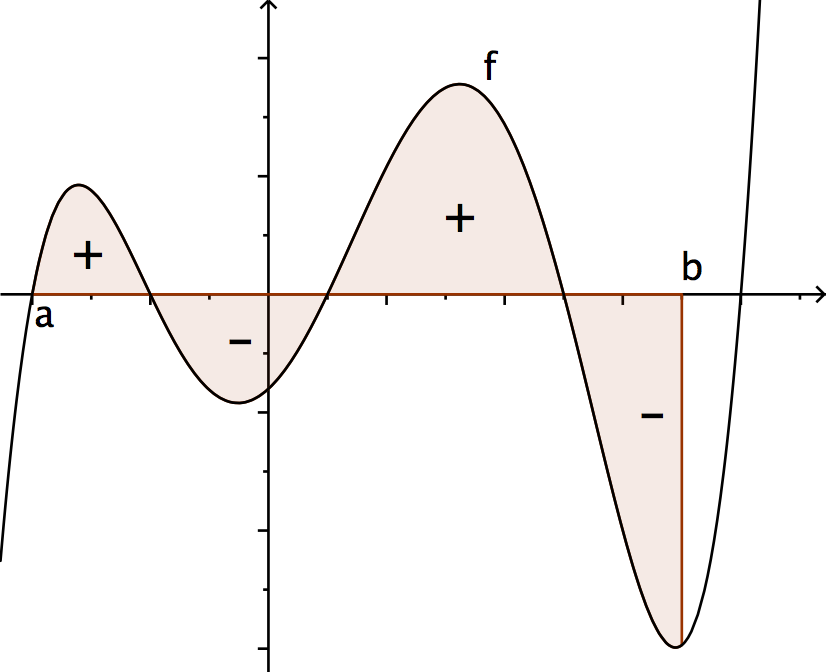
\includegraphics[width=\textwidth]{../Mathematik_2/Bilder/integration_vorzeichenbehafteter_flaecheninhalt.png}
\end{minipage}
	\hfill
	\begin{minipage}{0.5\textwidth}
		$\displaystyle{ \int\limits_{a}^b f(x)\, \mathrm{d}x}$ mit \ldots
\begin{itemize}
	\item Integrand $f(x)$,
	\item untere Integrationsgrenze $a$,
	\item obere Integrationsgrenze $b$,
	\item Differential $\mathrm{d}x$.
\end{itemize}
\end{minipage}
\end{defbox}

\begin{theorembox}{Eigenschaften des Integrals}{Aufgabe}
	\begin{enumerate}
	\item Das Integral eines Vielfachen (auch eines negativen Vielfachen!) einer Funktion ist das Vielfache des Integrals der Funktion:
		\[\forall C\, \in \mathbb R:\quad  \int\limits_a^b C\cdot f(x)\, \mathrm{d}x = C\cdot \int\limits_a^b f(x) \, \mathrm{d}x\,.\]
\item Das Integral der Summe zweier Funktionen ist die Summe der Integrale:
	\[\int\limits_a^b \left( f(x) + g(x) \right) \, \mathrm{d}x = \int\limits_a^b f(x) \, \mathrm{d}x + \int\limits_a^b g(x) \, \mathrm{d}x\,.\]
\item Das Integral ist bez�glich der Integrationsgrenzen additiv:
	\[\forall \, c\in [a,b]:\quad \int\limits_a^b f(x) \, \mathrm{d}x = \int\limits_a^c f(x) \, \mathrm{d}x + \int\limits_c^b f(x) \, \mathrm{d}x\,.\]
\item Vertauscht man die Integrationsgrenzen so �ndert sich das Vorzeichen des Integrals:
	\[\int\limits_a^b f(x) \, \mathrm{d}x = - \int\limits_b^a f(x) \, \mathrm{d}x\,.\]
%\item Es gilt also:
%	\[\int\limits_a^a f(x) \, \mathrm{d}x = 0\,.\]
	\end{enumerate}
\end{theorembox}

\noindent Bemerkungen:
\begin{itemize}
	\item Eine geometrische Fl�che ist immer positiv und das hei�t, dass das Integrationsgebiet entsprechend zu zerlegen ist, wenn man eine geometrische Fl�che als Integral berechnen m�chte!\marginpar{\small Aufgabe}
	\item Dass das Integral das Vorzeichen der Funktion ber�cksichtigt, f�hrt dazu, dass "\,Integration"\, eine \underline{lineare}\randverweis{MA1-matrizen} Abbildung ist!
	\item Das Integralzeichen $\int$ ist eigentlich ein langes S und steht f�r Summe, das Differential $\mathrm{d}x$ gibt die Variable an, �ber die integriert wird (hier $x$), und steht formal f�r eine unendliche kleine Differenz zweier verschiedener Werte $x_1$ und $x_2$.
\end{itemize}


Eine einfache Art, sich das Integral vorzustellen, ist die Fl�che unter dem Funktionsgraphen
in schmale Streifen zu zerlegen, diese durch Rechtecke anzun�hern und dann aufzusummieren.
Teilt man das Intervall \([a,b]\) in viele kleine Teilintervalle, so entstehen Rechteckn�herungen
der Fl�che.

\begin{defbox}{Ober- und Untersumme als Idee (+)}{}
Ist \(f:[a,b]\to\mathbb R\) nichtnegativ, so kann man in jedem Teilintervall
ein Rechteck mit der kleinsten vorkommenden H�he w�hlen. Die Summe dieser Rechtecksfl�chen
hei�t \textbf{Untersumme}. W�hlt man stattdessen die gr��te vorkommende H�he,
so erh�lt man die \textbf{Obersumme}.

Anschaulich gilt:
\[
\textnormal{Untersumme} \;\le\; \int_a^b f(x)\,\mathrm{d}x \;\le\; \textnormal{Obersumme}.
\]
Werden die Teilintervalle immer feiner, so n�hern sich diese Summen dem Integral an.
\end{defbox}

\noindent
Allgemeiner w�hlt man in jedem Teilintervall einen beliebigen St�tzpunkt \(t_i\)
und erh�lt eine \underline{Riemann-Summe}
\[
\sum_{i=1}^n f(t_i)\,\Delta x_i.
\]
F�r die in diesem Skript betrachteten Funktionen --- insbesondere f�r stetige und st�ckweise stetige Funktionen
auf endlichen Intervallen --- f�hrt diese Grenzwertidee auf das bestimmte Integral.

\noindent
\textbf{Bemerkung:}
F�r die praktische Rechnung ist diese Grenzwertkonstruktion nur selten entscheidend.
Wichtiger sind f�r uns:
\begin{itemize}
	\item der Hauptsatz der Differential- und Integralrechnung,
	\item die Rechenregeln f�r Integrale,
	\item und numerische N�herungsverfahren auf Basis endlich vieler Funktionswerte.
\end{itemize}


%Eine einfache Art, sich das Integral vorzustellen, ist die Fl�che unter der Funktion in schmale Streifen zu schneiden, diese als Rechtecke anzun�hern und dann aufzusummieren. Es gibt zwei M�glichkeiten Rechtecke zu bilden:
%\begin{itemize}
%	\item entweder schneidet man die $x$-Achse in kleine Streifen, oder,
%	\item man schneidet die $y$-Achse in kleine Streifen.
%\end{itemize}
%
%	\begin{figure}[h]\caption{links: Riemann-Integral, rechts: Lesbuege-Integral}
%\begin{center}
%	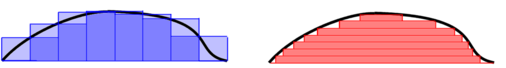
\includegraphics[width=0.8\textwidth]{../Mathematik_2/Bilder_unused/integration_riemann_und_lebesgue_vergleich.png}
%\end{center}
%\end{figure}
%
%Die erste Idee, links skizziert, f�hrt auf das { Riemann-Integral}. Die zweite Idee, rechts skizziert, f�hrt auf das {Lebesgue-Integral}.
%
%\noindent Bemerkungen:
%\begin{itemize}
%	\item Das Lebesgue-Integral ist allgemeiner und erlaubt die Integration von pathologischen Funktionen, beispielsweise der folgenden:
%\[ f: \mathbb R \to \mathbb R, \; x\mapsto \begin{cases} 1, \quad x\in \mathbb Q\,,\\ 0, \quad \mathbb R \setminus\mathbb Q\end{cases} \; \Rightarrow \forall\, a,b\in \mathbb R: \quad \int\limits_a^b f(x) \, \mathrm{d}x = 0\,.\]
%\item F�r die Praxis spielen die verschiedenen Definitionen des Integrals keine Rolle. Die Funktionen, die uns interessieren sind st�ckweise stetig und beschr�nkt und die lassen sich �ber jeden endlichen  Integrationsbereich  integrieren.  %Ausnahmen  dazu  gibt es  nur  in  bestimmten  mathematischen  Universen  (Suchbegriff:  Auswahlaxiom)  und/oder  in  Integralen  �ber  drei  oder  mehr  Dimensionen  (Suchbegriff: Banach-Tarski-Paradoxon).
%\end{itemize}
%
%Der Vollst�ndigkeit halber schlie�en wir diesen Absatz mit der Definition des Rieman-Integrals ab. Hierzu brauchen wir die Begriffe "\,Riemann-Summe"\, und "\,Riemann-Integrabilit�t"\,:
%\begin{defbox}{Riemann-Summe}{}
%Gegeben sei eine Funktion \(f:[a,b]\to\mathbb R\) und eine Zerlegung \(Z\) des Intervalls \([a,b]\) in St�tzstellen \(x_i, i=0,\cdots,n\), also:
%\[ Z = \bigcup_{i=1}^{n} [x_{i-1},x_i]\,,\]
%W�hlen wir in jedem Teilintervall eine beliebige Zwischenstelle \( t_i\in [x_{i-1}, x_i]\), so hei�t
%\[ S\left(f,Z, (t_i)_i\right) := \sum\limits_{i=1}^n f(t_i)\cdot \underbrace{(x_{i}- x_{i-1})}_{\displaystyle{=\Delta x_i}} \]
%die Riemannsche Summe von $f$ zur Zerlegung $Z$ mit Zwischenstellen $(t_i)_i$.
%\end{defbox}
%
%Die Riemann-Summe verallgemeinert die aus der Schule bekannten Ober- und Untersummen.
%
%\begin{defbox}{Riemann-Integrabilit�t}{}
%Gegeben sei eine Funktion \(f:[a,b]\to\mathbb R\) und eine Folge von Zerlegungen  \( (Z)_{n\in\mathbb N} \), f�r die gilt
%\[ \lim\limits_{n\to\infty} \delta_n = 0 \quad \textnormal{mit} \quad
%\delta_n := \max\limits_{1\leq i \leq n} \Delta x_i\,. \]
%W�hlen wir f�r jede Zerlegung in jedem Teilintervall eine beliebige Zwischenstelle \( \left( t^{(n)}_i\right)_{n\in\mathbb N}\), so hei�t
%\[ \left( S\left(f,Z, (t^{(n)}_i)_i\right)\right)_{n\in\mathbb N} \]
%Riemann-Folge von $f$. Die Funktion $f$ hei�t Riemann-integrierbar oder einfach nur integrierbar, falls jede Riemann-Folge von $f$ konvergiert.
%\end{defbox}
%
%Nun haben wir das Vokabular zusammen, um das Integral zu definieren:
%
%\begin{theorembox}{Riemann-Integral}{}
%Gegeben sei eine integrierbare Funktion \(f:[a,b]\to\mathbb R\). Dann haben alle Riemann-Folgen den gleichen Grenzwert $I\in \mathbb R$. Diesen Grenzwert nennen wir im folgenden Riemann-Integral bzw Integral und schreiben:
%\[ \int\limits_{a}^b f(x) \, \mathrm{d}x : = I\,.\]
%\end{theorembox}

\subsection{Hauptsatz der Differential- und Integralrechnung}

Der Wert des Integrals h�ngt von den Integrationsgrenzen $a$ und $b$ ab. Man kann das Integral also als Funktion beispielsweise von $b$ auffassen,
\[
	F: b\mapsto \int\limits_{a}^b f(x)\, \mathrm{d}x\,,
\]
und sich fragen, was die Ableitung von $F$ nach $b$ ist. Um die Frage zu beantworten, betrachten wir den \underline{Differenzenquotienten}\randverweis{MA1-stetigkeit-und-differenzierbarkeit}  und erhalten
\[
	\frac{F(b+h) - F(b)}{h}  = \frac{\int\limits_{a}^{b+h} f(x)\, \mathrm{d}x - \int\limits_{a}^{b} f(x)\, \mathrm{d}x}{h}= \frac{\int\limits_{b}^{b+h} f(x)\, \mathrm{d}x}{h}  \approx \frac{f(b)\cdot h}{h} =  f(b)\,.\quad (*)\,,
\]
wobei im letzten Schritt der wahre Fl�cheninhalt �ber dem Intervall \([b,b+h]\) durch die Fl�che des Rechtecks mit Seitenl�ngen $h$ und $f(b)$ abgesch�tzt wurde.

Die Ableitung hebt also in gewisser Weise das Integral auf und das k�nnen wir nutzen, um Integrale zu berechnen. Betrachten wir beispielsweise
	\[ \int\limits_{a}^b x^3 \, \mathrm{d}x\,.\]
	Wegen $(*)$ wissen wir, dass die Ableitung des Integrals von der oberen Grenze $b$ abh�ngt und $b^3$ sein muss:
\[
	\frac{\mathrm{d}}{\mathrm d b} \left( \int_a^b x^3\, \mathrm{d}x \right) \stackrel{!}{=} b^3 \Rightarrow   \int_a^b x^3\, \mathrm{d}x = \frac14 b^4 + C \,.
\]
Die letzte Gleichung muss auch f�r $b=a$ gelten, also:
\[
	 0 =  \int_a^a x^3\, \mathrm{d}x = \frac14 a^4 + C \Rightarrow  C=-\frac14 a^4 \,.
\]
Damit ist das Integral gel�st:
\[\int_a^b x^3\,\mathrm{d}x =  \frac14 \left( b^4 - a^4\right) \,.\]

Dieser Trick funktioniert immer und liefert ein Vorgehen zur Berechnung bestimmter Integrale:
	\begin{enumerate}
		\item Finde zum Integrand $f$ eine Funktion $F$ mit
			\[ F' = f\,.\]
		\item Berechne das Integral wie folgt:
		\[ \int\limits_a^b f(x) \, \mathrm{d}x = \Big[ F(x) \Big]_a^b = F(x)\Big|_a^b = F(b) - F(a)\,. \]
	\end{enumerate}

\noindent Bemerkungen:
\begin{itemize}
	\item Die Funktion $F$ nennt man Stammfunktion [antiderivative].
	\item Die Stammfunktion $F$ schreibt man auch oft als unbestimmtes Integral ohne Integrationsgrenzen.
		\item Stammfunktionen sind nur bis auf additive Konstanten eindeutig bestimmt.
		\item Das unbestimmte Integral ist eine \underline{Funktion}\randverweis{MA1-funktionen}, die von der Integrationsvariable abh�ngt.
		\item Das bestimmte Integral ist eine Zahl - n�mlich die vorzeichenbehaftete Fl�che unter dem Integrand.
	\end{itemize}

Der Zusammenhang zwischen Ableitung und Stammfunktion wird im sogenannten  Hauptsatz der Differential- und Integralrechnung [fundamental theorem of calculus] zusammengefasst.
\begin{theorembox}{Hauptsatz der Differtial und Inegralrechnung}{}
	F�r eine stetige Funktion $f:[a,b]\to\mathbb R$ gilt:
	\begin{itemize}
		\item F�r jede Stammfunktion $F$ von $f$ und alle $\alpha, \beta \in [a,b]$ gilt
			\[ \int\limits_{\alpha}^\beta f(x) \, \mathrm{d}x = F(\beta) - F(\alpha) =: \Big[ F(x) \Big]_\alpha^\beta\,.\]
			\item F�r $c\in[a,b]$ lautet eine  Stammfunktion von $f$:
				\[ F:[a,b]\to \mathbb R, x\mapsto F(x) = \int_c^x f(t) \, \mathrm{d}t\,.\]
		\end{itemize}
\end{theorembox}

Den Hauptsatz der Differential- und Integralrechnung kann man benutzen, um Integrale auszurechnen:\marginpar{\small Aufgabe}

\begin{exabox}{Hauptsatz der Differential und Integralrechnung}{ }
		\[ \int\limits_{0}^4 x^{-\frac12} \,\mathrm{d}x  = \Big[ 2 \sqrt{x}\Big]_0^4 = 4\,.
		\]
\end{exabox}

Um Stammfunktionen zu finden, stellt man eine Tabelle von Ableitungen auf und liest diese Tabelle r�ckw�rts. Wichtige Stammfunktionen sind die folgenden:

		\begin{center}
			\begin{tabular}{l|l||l|l || l| l}
				$f(x)$ & $F(x)$ & $f(x)$ & $F(x)$  & $f(x)$ & $F(x)$ \\
				\hline
				$r$ & $rx$ & $\cos(x)$ & $\sin(x)$ &  $\displaystyle{\frac{1}{\sqrt{1-x^2}}}$ & $\arcsin(x)$ \\
				$x^a, a\not=-1$ & $\displaystyle{\frac{x^{a+1}}{a+1}}$ & $\sin(x)$ & $-\cos(x)$ & $\displaystyle{\frac{-1}{\sqrt{1-x^2}}}$ & $\mathrm{arccos}(x)$  \\
				$\displaystyle{x^{-1}}$ & $\ln(|x|)$ & $\displaystyle{\frac{1}{\cos^2(x)}}$ & $\tan(x)$ & $\displaystyle{\frac{1}{1+x^2}}$ & $\arctan(x)$ \\
				$a^x, a>0$ & $\displaystyle{\frac{a^x}{\ln(a)}}$ & $\displaystyle{\frac{-1}{\sin^2(x)}}$  & $\mathrm{cot}(x)$ & $\displaystyle{\frac{-1}{1+x^2}}$ & $\mathrm{arccot}(x)$
			\end{tabular}
		\end{center}

\subsection{Uneigentliche Integrale}

Uneigentliche Integrale sind Integrale mit unbeschr�nktem Integrationsgebiet und/oder unbeschr�nktem Integranden. Die Frage, ob der Fl�cheninhalt unter dem Funktionsgraphen unter diesen Bedingungen eine endliche Zahl ist oder nicht, ist mit den bisherigen Mitteln nicht zu beantworten. Uneigentliche Integrale sind problematisch und man muss sie mit \underline{Grenzwertbetrachtungen}\randverweis{MA1-grenzwerte-von-folgen-und-funktionen} behandeln, um festzustellen, ob sie endlich, also definiert, sind.\marginpar{\small Aufgabe}
\begin{exabox}{Definierte uneigentliche Integrale}{ }
	\begin{eqnarray*}
		\displaystyle{\int\limits_0^\infty} e^{-x} \, \mathrm{d}x &=& \lim\limits_{M\to \infty}  \displaystyle{\int\limits_0^M} e^{-x} \, \mathrm{d}x = \lim\limits_{M\to \infty} \Big[ -e^{-x} \Big]_{0}^M =  \lim\limits_{M\to \infty} \left( -e^{-M} -(- 1) \right) = 1 < \infty\,, \\[2ex]
		\displaystyle{\int\limits_0^{16} \frac{1}{\sqrt{x}}} \, \mathrm{d}x &=& \lim\limits_{\varepsilon \downarrow 0} \displaystyle{\int_\varepsilon^{16} \frac{1}{\sqrt{x}}} \, \mathrm{d}x = \lim\limits_{\varepsilon \downarrow 0} \Big[ 2 \sqrt{x}\Big]_\varepsilon^{16} =  \lim\limits_{\varepsilon \downarrow 0} \left( 2 \sqrt{16} - 2\sqrt{\varepsilon} \right)  = 2\sqrt{16} = 8\,.
			\end{eqnarray*}
\end{exabox}

\begin{exabox}{Nicht-definierte uneigentliche Integrale}{ }
	\begin{eqnarray*}
		\displaystyle{\int\limits_0^\infty \sin(x)\, \mathrm{d}x} &=& \lim\limits_{M\to \infty} \displaystyle{\int_0^M \sin(x)\, \mathrm{d}x} = \lim\limits_{M\to \infty} \Big[ -\cos(x)\Big]_{0}^M = \lim\limits_{M\to \infty} \left(1 -\cos(M) \right)\; \textnormal{kein Grenzwert}\,, \\
		\displaystyle{\int\limits_0^{16} \frac{1}{x}  \, \mathrm{d}x } &=& \lim\limits_{\varepsilon \downarrow 0} \displaystyle{\int\limits_\varepsilon^{16} \frac{1}{x}  \, \mathrm{d}x }  = \lim\limits_{\varepsilon\downarrow 0} \Big[ \ln(|x|) \Big]_{\varepsilon}^{16} = \lim\limits_{\varepsilon\downarrow 0} \left( \ln(16) - \ln(\varepsilon)\right)\; \textnormal{kein Grenzwert}\,.
	\end{eqnarray*}
\end{exabox}

\subsection{Numerische Integration (+)}

Zu allen �blichen Funktionen l�sst sich schnell mit Hilfe von Produktregel, Kettenregel und so weiter die Rechenvorschrift der Ableitung hinschreiben. Mit Stammfunktionen ist das leider nicht so einfach. Zwei Probleme gibt es:

\begin{enumerate}
	\item Viele Funktionen haben keine Stammfunktion, die man mit �blichen Funktionen geschlossen hinschreiben kann. Die Glockenfunktion $x\mapsto e^{-x^2}$ beispielsweise l��t sich zwar integrieren, aber man findet keine Stammfunktion in Termen bekannten Funktionen.\marginpar{\small Aufgabe}
	\item Wenn man nur eine Reihe von Messdaten zur Verf�gung hat, dann kann man keine Stammfunktion bestimmen, weil keine Funktionsabbildung gegeben ist.
\end{enumerate}

Ohne Stammfunktion bleibt eigentlich nur die numerische Integration: Man sch�tzt die Fl�che unter der Kurve mit Hilfe endlich vieler Funktionswerte. Vorausgesetzt
\begin{itemize}
	\item das Integrationsintervall $[a,b]$ ist in kleine, gleich gro�e Streifen der Breite $h=(b-a)/N$ zerlegt:
		\[ x_k = \begin{cases}   a, &\quad k=0\,, \\ a+k\cdot h, &\quad 0< k < N \,,\\  b, &\quad k=N\,.\end{cases}\]
	\item und $f$ ist an den �quidistanten S�tzstellen $x_k$ bekannt:
		\[ y_k = \begin{cases}  f(a), \quad & k=0\,, \\ f(x_k)= f(a+k\cdot h), \quad &0< k < N \,,\\  f(b)\,, \quad &k=N\,,\end{cases}\]
\end{itemize}
dann l��t sich das bestimmte Integral durch die sogenannte Trapezformel ann�hern.\marginpar{ \small Aufgabe}
%Die Idee ist hier die kleinen Fl�chenst�cke unterhalb des Graphens mit Fl�cheninhalten $T_k$ der Trapeze anzun�hern:
%\[T_k = \frac{ y_{k+1}-y_{k}}{2}\cdot h\,.\]

\hspace{-0.7cm}\begin{minipage}{0.35\textwidth}
		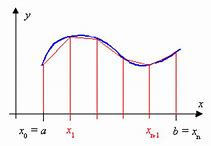
\includegraphics[width=1.0\textwidth]{../Mathematik_2/Bilder/integration_trapezregel_zerlegung.png}
\end{minipage}
\hspace{-0.5cm}\begin{minipage}{0.7\textwidth}
\begin{eqnarray*}
	\int\limits_{a}^b f(x)\, \mathrm{d}x &\approx& \frac{ f(x_1)+f(x_0)}{2}\cdot h + \frac{ f(x_2)+f(x_1)}{2}\cdot h  + \cdots + \\
&&+ \frac{ f(x_{N-2})+f(x_{N-1})}{2}\cdot h + \frac{ f(x_{N-1})+f(x_N)}{2}\cdot h\\
&&= h\cdot \left( \frac{f(x_0)}{2}  + \sum\limits_{k=1}^{N-1} f(x_k) + \frac{f(x_N)}{2}\right) := T_N(f)\,.
\end{eqnarray*}
	\end{minipage}

	\begin{theorembox}{Trapezformel}{}
		Trapezformel f�r $f:[a,b]\to \mathbb R$:
		\begin{eqnarray*}
			\int\limits_{a}^b f(x)\, \mathrm{d}x \approx T_N(f) = h\cdot  \left( \frac{f(x_0)}{2}  + \sum\limits_{k=1}^{N-1} f(x_k) + \frac{f(x_N)}{2}\right) \,.
		\end{eqnarray*}
		Fehlerabsch�tzung f�r $f'':[a,b]\to \mathbb R$ stetig:
		\begin{eqnarray*}
		\exists\, \xi \in [a,b]:\quad  \Big| T_N(f) - \int_a^b f(x)\Big|  = \frac{(b-a)\cdot f''(\xi)}{12} \cdot h^2
	\end{eqnarray*}
\end{theorembox}

\begin{exabox}{Trapezformel}{ }
Gesuchter Integralwert:
			\[
				\displaystyle{ \int\limits_{0}^\pi \sin(x) \,\mathrm{d}x} = \Big[ -\cos(x)\Big]_0^\pi = 2\,.
			\]
Trapezformel f�r $N=4$:
			\begin{eqnarray*} T_4(\sin) = \frac{\pi}{4}\left( \frac12 \sin\left(0\cdot \frac{\pi}{4}\right)  + \sin\left( 1\cdot \frac{\pi}{4}\right) + \sin\left( 2\cdot \frac{\pi}{4}\right) + \sin\left( 3\cdot \frac{\pi}{4}\right)   + \frac12\sin\left( 4\cdot \frac{\pi}{4}\right) \right) \approx 1.896 \,.
			\end{eqnarray*}
\end{exabox}

Mit  asymptotisch  gleichem Rechenaufwand  kann  man  die Funktion  sogar  durch  St�cke  kubischer  (nicht  nur  quadratischer!)  Parabeln ann�hern und erh�lt die Simpson-Formel. �ber jedem Intervall der Breite $h$ zieht man zur Approximation des Fl�cheninhalts neben den St�tzstellen an den Intervallenden noch die Intervallmitte heran.

\begin{theorembox}{Simpsonformel}{}
%\begin{minipage}{0.3\textwidth}
%	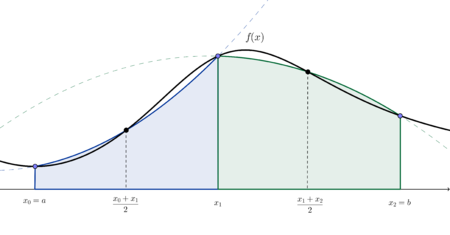
\includegraphics[width=\textwidth]{../Mathematik_2/Bilder_unused/integration_simpsonregel_parabelnaeherung.png}
%\end{minipage}
%\begin{minipage}{0.4\textwidth}

Simpsonformel f�r $f:[a,b]\to \mathbb R$ stetig:
\begin{eqnarray*}
	\int\limits_{a}^b f(x)\, \mathrm{d}x &\approx& S_N(f) :=  \frac{h}{6} \left( f(x_0)+ 4\cdot  f\left( \displaystyle{\frac{x_1 + x_0}{2}}\right) + 2\cdot f(x_1) + 4 \cdot f\left( \displaystyle{\frac{x_2 + x_1}{2}}\right) + \right.\\
	&&\left. + \cdots 2\cdot f(x_{N-1}) + 4\cdot f\left( \displaystyle{\frac{x_{N-1} + x_{N}}{2}}\right) + f(x_{N})\right) \,.
\end{eqnarray*}
Fehlerabsch�tzung f�r $f^{(4)}:[a,b]\to \mathbb R$ stetig:
		\begin{eqnarray*}
			\exists\, \xi \in [a,b]:\quad  \Big| S_N(f) - \int_a^b f(x)\Big| = \frac{(b-a)\cdot f^{(4)}(\xi)}{2880} \cdot h^4
	\end{eqnarray*}
	%\end{minipage}
\end{theorembox}

\noindent Bemerkungen:
\begin{itemize}
	\item Eine Verbesserung des Trapezverfahrens ist das sogenannte das Romberg-Verfahren. Das Romberg-Verfahren nutzt das Trapezverfahren f�r verschiedene Schrittweiten.

	\item Die naheliegendste Formel zur numerischen Integration ist die Summe von Rechtecken zu bilden (zum Beispiel Ober- oder Untersumme). Das Preis-Leistungs-Verh�ltnis dieser Rechteck-Verfahren ist allerdings schlecht im Vergleich zur Trapezformel.\marginpar{\small Aufgabe}
\end{itemize}
 \newpage % 04 Hauptsatz der Integralrechung
%\setcounter{exercise}{0} \ifintegriereaufgaben
\section*{Integral Aufgaben}\label{MA2-integration-aufgaben}

Erkl�rungen und Beispiele, die zur Bearbeitung der Aufgaben hilfreich sind, finden Sie im Skript\wennreferenzvorhanden{MA2-integration}{ (Abschnitt \abschnittsverweis{MA2-integration})} und, falls Sie nicht weiterkommen, dann schauen Sie \hyperref[MA2-integration-loesungen]{hier}.
\else
\section{Integral Aufgaben}\label{MA2-integration-aufgaben}

Regeln und Beispiele zu diesen Aufgaben finden Sie im Skript. Die L�sungen finden Sie \hyperref[MA2-integration-loesungen]{hier}.
\fi

\begin{exercisebox}[Fl�cheninhalt]
	Berechnen mit Hilfe geometrischer �berlegungen den Fl�cheninhalt zwischen den Graphen und $x$-Achse
	\small{
	\begin{eqnarray*}
		(a) \;  \displaystyle{ \int\limits_0^4} (2x-1) \mathrm{d}x \quad  \quad  (b) \; \displaystyle{ \int\limits_0^2} (x-1)^3 \mathrm{d}x  \quad \quad (c) \; \displaystyle{ \int\limits_0^1} |\sin(2\pi x)| \mathrm{d}x
\end{eqnarray*}}
\end{exercisebox}

\begin{exercisebox}[Fl�cheninhalt (Trapezformel)] % LS p 153
\begin{itemize}
	\item[(a)] $A$ sei der Fl�cheninhalt eines Kreises mit Radius $r$. Zeigen Sie: $ 2r^2 < A < 4 r^2$.
	\item[(b)] Entwickeln Sie eine Methode zur Bestimmung von $A$ und implementieren Sie diese (Matlab, Excel).
	\item[(c)] Was ist der Unterschied zur Fl�cheninhaltsberechnung von Vielecken?
\end{itemize}
\end{exercisebox}

\begin{exercisebox}[Eigenschaften des Integrals]
	Begr�nden Sie, dass jede Integralfunktion $ F(x):= \displaystyle{\int\limits_{a}^x} f(t)\,\mathrm{d}t$ mindestens eine Nullstelle hat.
\end{exercisebox}

\begin{exercisebox}[Hauptsatz der Differential- und Integralrechnung]  %Papula 1, V, Abschnitt 1-7, Aufgaben Seite 559, L�sungen Seite 787
	Bestimmen Sie alle Stammfunktionen folgender Funktionen:
	\begin{eqnarray*}
		\begin{array}{l l l }
			(a) \;  x\mapsto 4x^5-6x^3+8x^2-3x +5
			& (b) \; x\mapsto e^x + x^2 - 2x + \sin(x)
			& (c)\; x\mapsto \displaystyle{\frac{\tan(x)}{\sin(2x)}}
		\end{array}
	\end{eqnarray*}
%\end{itemize}
\end{exercisebox}

\begin{exercisebox}[Bestimmte und uneigentliche Integrale] %Papula 1, V, Abschnitt 1-7, Aufg. 3 Seite 560, L�sungen Seite 787ff
	% https://mathematikalpha.de/wp-content/uploads/2016/05/aufg125.pdf
	Bestimmen Sie die Werte der folgenden Integrale, vorausgesetzt sie existieren:
	\begin{eqnarray*}
		\hspace{-0.3cm}
		\begin{array}{l l l l}
			(a) \; \displaystyle{\int_0^4} \left( x^3 - 5x^2 + \frac32 x -10\right)\, \mathrm{d}x & (b)\; \displaystyle{\int_1^4} \displaystyle{\frac{1-z^2}{z}}\,\mathrm{d}z &(c)\; \displaystyle{\int_0^{0,5}} \displaystyle{\frac{3}{\sqrt{1-x^2}}}\, \mathrm{d}x & (d)\; \displaystyle{\int_0^{\pi/4}} \displaystyle{\frac{1-\cos^2(x)}{2\cos^2(x)}}\,\mathrm{d}x \\[2ex]
			(e) \; \displaystyle{\int_1^\infty} \frac{1}{x^4}\,\mathrm{d} x & (f)\; \displaystyle{\int_0^\infty} \displaystyle{\frac{1}{x}}\,\mathrm{d}x  & (g)\; \int\limits_{-\infty}^0 e^{-t}\,\mathrm{d}t &(h)\; \displaystyle{\int_0^{4}} \displaystyle{\frac{2}{\sqrt{t}}}\, \mathrm{d}t
		\end{array}
	\end{eqnarray*}
\end{exercisebox}

\begin{exercisebox}[Numerische Integration]
	Das folgende bestimmte Integral soll n�herungsweise bestimmt werden:
	\[
		\int_1^3 x^3 \, \mathrm{d}x = 20\,.
	\]
	Bestimmen Sie eine Zerlegung des Intervalls $[1,3]$ in $4$ gleich gro�e Intervalle. Approximieren Sie das Integral mit Hilfe einer Rechteckregel, mit Hilfe der Trapezregel und mit Hilfe der Simpson-Regel.
\end{exercisebox}

\begin{exercisebox}[Simpson-Regel]
	%\begin{itemize}
		%\item[(a)] Berechnen SIe \[ \int\limits_0^2 \left( 4x^3+3x^2-4x-1\right)\,\mathrm{d}x \] mit der Simpson-Regal. Welchen absoluten Fehler erwarten Sie? �berpr�fen Sie Ihre Vermutung durch analytische Berechnung des Integrals.
		%\item[(b)]
	Bestimmen Sie den relativen Fehler, den Sie bei einer Approximation des Intgrals \[ \int\limits_0^1 x\cdot \cos(x^2) \, \mathrm d x\] mit Hilfe der Simpson-Regel auf drei �quidistanten Teilintervallen machen.
	%\end{itemize}
\end{exercisebox}

%\subsection{Praxis}

%\begin{exercisebox}[Ableitungen] % Papula 1, V, Abschnitt 1-2, Aufg. 6 % p. 174
%	Bestimmen Sie die folgenden Ableitungen
%	\begin{eqnarray*}
%			(a) \; f: x\mapsto e^{\sin(x)} + C  \quad
%			(b)\; f: x\mapsto \displaystyle{\frac16} \sin^2(3x) + C
%			(c)\; f: x\mapsto \displaystyle{\int_{-5}^x} (t^2-2t)\,\mathrm{d}t + C
%			(d)\; f: x\mapsto \displaystyle{\int_{x}^0} (t^2-2t)\,\mathrm{d}t + C
%			(e)\; f: x\mapsto \displaystyle{\int_{0}^x} (t^2-2t)\,\mathrm{d}t + C
%		\end{array}
%	\end{eqnarray*}
%%\vspace{0.3cm}
%%{\bf L�sung:} Differenziere die rechte Seite.
%\begin{itemize}
%	\item[(a)] $\cos(x) \cdot e^{\sin(x)} $
%	\item[(b)] $\sin(3x) \cdot \cos(3x) $
%	\item[(c)] $x^2-2x$
%	\item[(d)] $-x^2+2x$
%	\item[(e)] $x^2-2x$
%\end{itemize}
%\end{exercisebox}

%\begin{exercisebox}[Eigenschaften des Integrals] % p. 174
%	Bestimmen Sie obere Grenze $b$ bzw. die untere Grenze $a$
%	\begin{eqnarray*}
%			(a)\; \displaystyle{\int_{a}^5} x^2\,\mathrm{d}t = 63
%			(b)\; \displaystyle{\int_{1}^b} 2x^3\,\mathrm{d}x = 9
%			(c)\; \displaystyle{\int_{a}^{10}} \frac{1}{x^2}\,\mathrm{d}x = 0,5
%		\end{array}
%	\end{eqnarray*}
%%%\vspace{0.3cm}
%%%{\bf L�sung:}
%%\begin{itemize}
%%	\item[(a)] $a=-4$
%%	\item[(b)] $b=3$
%%	\item[(c)] $a=5/3$
%%\end{itemize}
%\end{exercisebox}

%\begin{exercisebox}[Fl�cheninhalt]
%	Berechnen mit Hilfe von geometrischen �berlegungen den Fl�cheninhalt zwischen Graphen und $x$-Achse
%	\begin{eqnarray*}
%	\displaystyle{\int\limits_0^{2\pi}} \sin(k x)\cdot \cos(k x) \mathrm{d}x
%		\end{array}
%\vspace{0.3cm}
%{\bf L�sung:} \newline
%$ A = 0$
%\end{itemize}
%\end{exercisebox}

%\begin{exercisebox}[Eigenschaften des Integrals] % Papula, Abschn. 1-7, Aufg. 5
%	Es gelte
%	\[ \int\limits_0^{1} f(x) \mathrm{d}x = 3 \land \int\limits_0^{2} f(x) \mathrm{d}x = 9\,. \]
%	Mit diesen Informationen l��t sich der Integralwert \[ \displaystyle{ \int\limits_{1}^2} f(x)\, \mathrm{d}x\] bestimmen - wie lautet er?
%\vspace{0.3cm}
%{\bf L�sung:} \newline
%\begin{eqnarray*}
%	\int\limits_1^2 f(x)\,\mathrm{d}x &=& - \int\limits_0^1 f(x)\, \mathrm{d}x + \int\limits_0^1 f(x)\, \mathrm{d}x + \int\limits_1^2 f(x)\, \mathrm{d}x \\
%	&=& - \int\limits_0^1 f(x)\, \mathrm{d}x + \int_0^2 f(x) \, \mathrm{d}x = -3 + 9 = 6\,.
%\end{eqnarray*}
%\end{exercisebox}

%\begin{exercisebox}[Fl�cheninhalt] % p. 175
%Gegeben ist die Funktion \(f\) mit \(f:x\mapsto 2- \displaystyle{ \frac{2}{x^2+1}}\).  Skizzieren Sie den Graphen von \(f\).
%\begin{itemize}
%	\item[(a)] Bestimmen Sie alle Stellen \(x\), f�r die gilt.
%\[ 2-\frac{2}{x^2} < f(x) \].
%	\item[(b)] Der Graph von \(f\), die \(x\)-Achse und die Geraden mit den Gleichungen \(x=4\) und \(x=10\) begrenzen eine Fl�che. Geben Sie an, wie gro� der Inhalt diese Fl�che mindestens ist.
%\end{itemize}
%%\vspace{0.3cm}
%%{\bf L�sung:}
%\begin{itemize}
%	\item[(a)] $-\infty < x < \infty$
%	\item[(b)]
%Es gilt
%\begin{eqnarray*}
%	x^2 < x^2+1 \Leftrightarrow \frac{1}{x^2} > \frac{x^2+1} \Leftrightarrow -\frac{1}{x^2} < -\frac{x^2+1} \Leftrightarrow 2 -\frac{1}{x^2} < 2-\frac{x^2+1} \Rightarrpw A \geq \int\limits_{4}^{10} \left( 2- \frac2{x^2}\right) \,\mathrm{d}x = 11,7
%\end{eqnarray*}
%\end{itemize}
%\end{exercisebox}

%\begin{exercisebox}{Hauptsatz der Differential- und Integralrechnung}{ }  %Papula 1, V, Abschnitt 1-7, Aufg. 1
%	Bestimmen Sie alle Stammfunktionen folgender Funktionen:
%	\begin{eqnarray*}
%		\begin{array}{l l l }
%			(a)\; x\mapsto \displaystyle{\frac{1-2x^2-4x^3}{2x}} + 3 & (b)\; z\mapsto \displaystyle{\frac{5}{3+3z^2}} -\displaystyle{\frac14}z^4 & (c)\; x\mapsto -3 e^x - \cos(x)  \\
%			(d)\; x\mapsto \sqrt{x \sqrt{x}} & (e)\; t\mapsto -\displaystyle{\frac{3}{1+t^2}} - \displaystyle{\frac1t} &
%		\end{array}
%	\end{eqnarray*}
%\vspace{0.3cm}
%{\bf L�sung:} \newline
%\begin{itemize}
%	\item[(a)] $F(x) = \displaystyle{\frac12} \ln(|x|) - \displaystyle{\frac12}x^2 - \displaystyle{\frac23} x^3 + 3 x + C $
%	\item[(b)] $F(z) = \displaystyle{\frac53} \arctan(z) - \displaystyle{\frac{1}{20}}z^5 + C $
%	\item[(c)] $F(x) = -3 e^x - \sin(x) + C $
%Papula 1, V, Abschnitt 1-7, Aufg. 2
%	\item[(d)] $F(x) =- 3 \arctan(t) - \ln(|t|) + C $
%	\item[(e)] $F(z) = \displaystyle{\frac47} x^{7/4} + C $
%\end{itemize}
%\end{exercisebox}

%\begin{exercisebox}[Fehler numerischer Verfahren]
%Betrachten Sie das folgende Integral
%\[
%	\int\limits_{-10}^{10} e^{-x^2}\,\mathrm{d}x\,.
%\]
%Approximieren Sie den Integralwert mit Hilfe der Trapezformel. Wie fein muss die Zerlegung sein, um einen relativen Fehler von \( 1\%\) zu erreichen? Benutzen Sie zur Fehlerberechnung den exakten Wert des Integrals erf(x). Schreiben Sie hierzu ein Program.
%\vspace{0.3cm}
%{\bf L�sung:}
%\end{exercisebox}

%\begin{exercisebox}[Fehler numerischer Verfahren]
%Betrachten Sie das folgende Integral
%\[
%	\int\limits_{-5}^2 \left( 4x^3+2x-\pi\right)\,\mathrm{d}x\,.
%\]
%Zu untersuchen ist die G�te unterschiedlicher numerischer Integrationsverfahren. Approxieren Sie den Integralwert f�r eine �quidistante Zerlegung des Intervalls in drei Teile, also \(n=3\) mit
%\begin{itemize}
%	\item der Obersumme
%	\item der Trapezformel
%	\item Simpson-Formel exakt f�r kubische Funktionen
%\end{itemize}
%Wie fein muss die Zerlegung mindestens sein, um mit der Trapezformel einen relativen Fehler von \( 1\%\) zu erreichen? Schreiben Sie hierzu ein Program.
%Bestimmen Sie eine Approximation an den Integralwert f�r eine �quidistante Zerlegung des Intervalls in drei Teile, also \(n=3\)
%\begin{itemize}
%	\item Trapezformel exakt f�r lineare Funktionen
%	\item Simpson-Formel exakt f�r kubische Funktionen
%	\item Obersumme f�r nichts exakt
%\end{itemize}
%%\vspace{0.3cm}
%%{\bf L�sung:}
%\begin{itemize}
%	\item Trapezformel ist exakt f�r lineare Funktionen
%	\item Simpson-Formel ist exakt f�r kubische Funktionen
%	\item Obersumme f�r nichts exakt
%\end{itemize}
%\end{exercisebox}


%\begin{exercisebox}[Zwischenwertsatz]
%	Bestimmen Sie eine Zwischenstelle $\xi\in (0,a)$, so dass f�r $f: x\mapsto x^2$ folgendes gilt
%	\[ \int\limits_0^a f(x) \mathrm{d}x =  a\cdot f(\xi)\,.\]
%\vspace{0.3cm}
%{\bf L�sung:} \newline
%Es gilt
%\begin{eqnarray*}
%	\int\limits_0^a f(x)\,\mathrm{d}x = \int\limits_0^a x^2\, \mathrm{d}x \Rightarrow  \quad \xi\in(0,a): \xi^2 \cdot a \stackrel{!}{=} \frac13 a^3 \Rightarrow \xi = \frac{a}{\sqrt{3}}\,.
%\end{eqnarray*}
%\end{exercisebox}


%\begin{exercisebox}[Numerische Integration]
%		Schreiben Sie allgemein ein Programm zur n�herungsweisen Berechnung von \[ \int\limits_a^b f(x) \, \mathrm{d}x \]
%		mithilfe der summierten Trapezregel mit $n\in\mathbb N$ Unterteilungen des Intervalls. Folgende Funktionen sollen damit n�herungsweise integriert werden:
%		\[ \int\limits_1^3 x^3 \, \mathrm{d}x,\quad \int\limits_0^1 \sqrt{x}\,\mathrm{d}x, \quad \int\limits_1^2\sqrt{x}\,\mathrm{d}x\,.\]
%		Gehen Sie dabei wie folgt vor:
%	\begin{itemize}
%		\item[(a)] Berechnen Sie f�r $n=10, 100, 10000$ eine Approximation des Integrals und berechnen Sie den absoluten Fehler $e_n$.
%		\item[(b)] Tragen Sie dann den absoluten Fehelr $e_n$ logarithmisch �ber die Anzahl $n$ auf und bestimmen Sie graphisch die Ordnung $k$ f�r die ein $C$ existiert, so dass
%			\[ e_n \leq C\cdot n^{-k} \]
%			gilt Wie erkl�ren Sie sich die Unterschiede?
%
%	\end{itemize}
%%\vspace{0.3cm}
%%{\bf L�sung:} \newline
%%\begin{itemize}
%%\end{itemize}
%\end{exercisebox}

 \newpage
\setcounter{def}{0} \setcounter{satz}{0} \setcounter{exa}{0} \section{Integrationsregeln}\label{MA2-integrationsregeln}

\begin{table}[H]
  \centering
  \begin{tabularx}{\textwidth}{@{}>{\raggedright\arraybackslash}X r@{}}
    \toprule
    \multicolumn{2}{c}{\textbf{�bersicht �ber Lernziele und Voraussetzungen}} \\
    \midrule
    \textbf{Lernziele} & \\[.5\normalbaselineskip]
    \tabitem bestimmte Integrale �ber st�ckweise stetige Funktionen korrekt zerlegen und berechnen & \\
    \tabitem unbestimmte Integrale mit Substitution und partieller Integration bestimmen & \\
    \tabitem rationale Funktionen mittels Partialbruchzerlegung integrieren & \\
    \tabitem rationale Funktionen mittels Partialbruchzerlegung integrieren & \\[.5\normalbaselineskip]
    \midrule
    \textbf{Voraussetzungen} &  \\[.5\normalbaselineskip]
    \tabitem die Eigenschaften des Integrals anwenden k�nnen & \abschnittsverweis{MA2-integration}  \\
    \tabitem die Ketten-, Produkt- und Quotientenregel anwenden k�nnen & \abschnittsverweis{MA1-ableitungsregeln} \\
    \tabitem mit komplexen Zahlen sicher umgehen k�nnen & \abschnittsverweis{MA1-komplexe-zahlen-polarform-und-euler}  \\
    \tabitem Partialbruchzerlegungen durchf�hren k�nnen & \abschnittsverweis{MA2-partialbruchzerlegung} \\[.5\normalbaselineskip]
    \bottomrule
  \end{tabularx}
\end{table}

\noindent \ifintegriereaufgaben Die �bungsaufgaben zum Thema finden Sie \hyperref[MA2-integrationsregeln-aufgaben]{hier}.
\vspace{0.3cm}
\hrule
\fi

\subsection{Integration st�ckweise stetiger Funktionen}

Neben den elementaren Integrationstechniken, die sich aus den Eigenschaften des Integrals ergeben, gibt es Tricks und wichtige Regeln, die in diesem Kapitel vorgestellt werden.\marginpar{\small Aufgaben}


Wenn der Integrand $f:[a,b]\to\mathbb R$ auf $[a,b]$ einen Knick macht oder st�ckweise definiert ist, dann hei�t es nicht, dass man keine Stammfunktion finden kann. In diesen Fall kann es helfen das Integrationsgebiet zu zerlegen. Findet man in jedem Teilintervall eine Stammfunktion, dann kann man das Integral berechnen.

\begin{exabox}{Integration durch Zerlegung des Integrationsgebiets}{ }
Integral:
\[ \displaystyle{\int\limits_{-2}^2} |x-1|\,\mathrm{d}x = \textnormal{?}\]
	Stammfunktionen:
	\[
		\begin{cases}
			F_1(x) = x -\displaystyle{ \frac12 }x^2 + C, \quad & x\in[-2,1]\,, \\
			F_2(x) = \displaystyle{ \frac12 }x^2 -x + C, & x \in [1,2]\,.
		\end{cases}
	\]
	L�sung:
	\[ \int\limits_{-2}^2 |x-1|\,\mathrm{d}x = \Big[ F_1(x)\Big]_{-2}^1 +  \Big[ F_2(x)\Big]_{1}^2 = 1-\frac12 - (-2) + \frac12\cdot 4 + \frac12 \cdot 4 -2 - \frac12 + 1 = 5\,.
	\]
\end{exabox}

\begin{exabox}{Integration durch Zerlegung des Integrationsgebiets}{ }
Integral:
\[ \displaystyle{\int\limits_{0}^2} f(t)\,\mathrm{d}t = \textnormal{?} \quad \textnormal{mit}\quad f:t\mapsto \begin{cases} 2e\cdot t, \quad & t< 1\,,\\ 2e^t, & t\geq 1\,.\end{cases} \]
	Stammfunktionen:
	\[
		\begin{cases}
			F_1(t) = t^2 e + C, \quad & t\in[0,1]\,, \\
			F_2(t) =  2e^t + C,  &t \in [1,2]\,.
		\end{cases}
	\]
	L�sung:
	\[ \int\limits_{0}^2 f(t)\,\mathrm{d}t = \Big[ F_1(t)\Big]_{0}^1 +  \Big[ F_2(t)\Big]_{1}^2 = e+2e^2-2e = 2e^2 -e\,.
	\]
\end{exabox}

Wenn der Integrand $f$ auf $[a,b]$ nicht stetig, aber st�ckweise stetig ist, dann kann man genauso vorgehen. Zuerst die Definition einer st�ckweise stetigen Funktion und dann die Verallgemeinerung der Integrationstechnik.
\begin{defbox}{St�ckweise stetige Funktionen}{}
	\hspace{-0.3cm}\begin{minipage}{0.4\textwidth}
		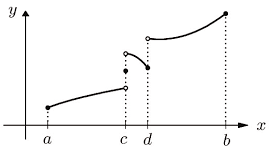
\includegraphics[width=\textwidth]{../Mathematik_2/Bilder/integration_stueckweise_stetige_funktion.png}
\end{minipage}
	\begin{minipage}{0.6\textwidth}
	$f$ ist auf $[a,b]$ st�ckweise stetig, das hei�t:
	\begin{itemize}
		\item $f$ ist bis auf h�chstens endlich viele Punkte $x_1, \cdots, x_n\in [a,b]$ stetig,
		\item der links- und der rechtsseitige Grenzwert an allen Punkten $x\in (a,b)$ existiert,
		\item der rechtsseitige Grenzwert am linken Intervallende existiert und
		\item der linksseitige Grenzwert am rechten Intervallende existiert.
	\end{itemize}
\end{minipage}
\end{defbox}

\begin{theorembox}{Integration st�ckweise stetiger Funktionen}{}
	Es sei $f:[a,b]\to\mathbb R$ st�ckweise stetig mit $n$ Unstetigkeitsstellen $x_k\in[a,b], k=1,\cdots,n,$ und $a=x_0<x_1<x_2< \cdots < x_n<x_{n+1}=b$. Dann ist $f$ integrierbar �ber $[a,b]$ mit
	\[ \int\limits_a^b f(x)\,\mathrm{d}x = \sum\limits_{k=1}^{n+1}\int\limits_{x_{k-1}}^{x_k} \overline f_k(x) \,\mathrm{d}x\,,\]
	wobei $\overline f_k$ die stetige Fortsetzung von $f$ im Intervall $[x_{k-1}, x_k]$ bezeichnet.
\end{theorembox}

\subsection{Integration von Produkten}

Wie kann man die \underline{Produktregel}\randverweis{MA1-ableitungsregeln} der Ableitung r�ckw�rts lesen, um etwas �ber ein Integral zu erfahren?
\[
	\left( f\cdot g\right)' = f'\cdot g + f\cdot g'\,.
\]
Die Produktregel gibt uns eine Stammfunktion f�r $f'g+f g'$. Also kann man das bestimmte Integral dieser Funktion ausrechnen:
	\[
		\int\limits_{a}^b \left(  f'(x)\cdot g(x) + f(x)\cdot g'(x)\right) \, \mathrm{d} x = \Big[ f(x) \cdot g(x) \Big]_{a}^b \,.
	\]

Umstellen liefert die partielle Integration [integration by parts]:
	\[
		\int\limits_{a}^b f'(x)\cdot g(x)  \, \mathrm{d} x = \Big[ f(x) \cdot g(x) \Big]_a^b  -  \int\limits_a^b f(x)\cdot g'(x) \, \mathrm{d} x\,.
	\]

Grob gesagt, kann man also im Integral eine Ableitung auf den anderen Faktor �berw�lzen, wenn man das Vorzeichen �ndert und noch einen Randterm dazuschreibt. Die entsprechende Stammfunktion lautet also:
\begin{theorembox}{Partielle Integration}{}
	\[
		\int f'(x)\cdot g(x)  \, \mathrm{d} x = f(x) \cdot g(x)  -  \int f(x)\cdot g'(x) \, \mathrm{d} x + C\,.
	\]
\end{theorembox}

Partielle Integration ist dann praktisch, wenn die zu integrierende Funktion ein Produkt zweier Faktoren ist, von denen einer durch Ableiten deutlich einfacher und der andere durch Integrieren nicht schlimmer wird.
\begin{exabox}{Partielle Integration}{}
	\[
		\int  \cos(x) \cdot x  \, \mathrm{d} x = \sin(x)\cdot x - \int \sin(x) \, \mathrm{d} x + C = x \sin(x)+\cos(x) + C\,.
	\]
\end{exabox}

%Beispiel: $\int_3^5 x \cos(x) \, \mathrm{d}x=5$ Wolfram  Alpha  f�hrt  das  vor,  wenn  man  statt  des  bestimmten  Integrals \begin{verbatim} integrate x cos(x) from 3 to 5 \end{verbatim} das  unbestimmte  Integral \begin{verbatim} integrate x cos(x) \end{verbatim} abfragt und dann auf \begin{verbatim} Show steps\end{verbatim} klickt.


\subsection*{Integration komplexwertiger Funktionen}

Auch komplexwertige Funktionen lassen sich integrieren.
Die Grundidee ist einfach:
Man integriert Real- und Imagin�rteil getrennt.

\begin{defbox}{Integration komplexwertiger Funktionen}{}
Ist \(f : [a,b] \to \mathbb C\) gegeben durch
\[
f(x)=u(x)+i\,v(x)
\qquad\textnormal{mit}\qquad
u,v:[a,b]\to\mathbb R,
\]
so definiert man
\[
\int_a^b f(x)\,dx
:=
\int_a^b u(x)\,dx
+i\int_a^b v(x)\,dx.
\]
Entsprechend ist \(F\) genau dann eine Stammfunktion von \(f\),
wenn \(F'(x)=f(x)\) gilt.
\end{defbox}

\noindent
Der Vorteil dieser Sichtweise m�ndet nicht in eine neue Rechenregel, sondern in einen Fahrplan, um trigonometrische Funktionen zu integrieren. Das, was wir brauchen ist die \underline{Eulersche Identit�t}\randverweis{MA1-komplexe-zahlen-polarform-und-euler} in einer der folgenden Varianten
\[ e^{ix}= \cos(x) + i\sin(x),\qquad \sin(x) = \frac{1}{2i} \left( e^{ix}-e^{-ix}\right), \qquad \cos(x) = \frac{1}{2} \left( e^{ix}+e^{-ix}\right).\]


\begin{exabox}{�bergang in die komplexe Ebene}{}
Gesucht ist eine Stammfunktion von
\[
x \mapsto e^{-x}\cdot \cos(x).
\]

Mit der Eulerschen Identit�t
\[
e^{ix}=\cos(x)+i\sin(x)
\]
folgt
\[
	e^{-x}\cdot \cos(x) = \mathrm{Re}\left( e^{(-1+i)x} \right)
\]
Wir bestimmen zun�chst die Stammfunktion f�r die komplexe Exponentialfunktion und bestimmen im anschluss nur den Realteil - das ist die L�sung des Ausgangsintegrals.
\begin{enumerate}
	\item Komplexe Exponentialfunktion integrieren:
\[
	F(x) = \int e^{(-1+i)x}\,\mathrm dx = \frac{1}{-1+i}\,e^{(-1+i)x}+C = \left(-\frac12-\frac12 i\right)\, e^{(-1+i)x}+C,
\]
	\item Realteil ermitteln: mit
\[
e^{(-1+i)x}=e^{-x}\cdot \bigl(\cos(x)+i\sin(x)\bigr)
\]
ergibt sich
\[
\begin{aligned}
\left(-\frac12-\frac12 i\right) e^{(-1+i)x}
&= -\frac12 e^{-x}\bigl(\cos(x)-\sin(x)\bigr) \\
&\quad -\frac12 i\,e^{-x}\bigl(\sin(x)+\cos(x)\bigr).
\end{aligned}
\]
Daraus folgt f�r den Realteil:
\[
\mathrm{Re}\left(F(x)\right) = -\frac12 e^{-x}\bigl(\cos(x)-\sin(x)\bigr).
\]
\item Gesuchte Stammfunktion aufschreiben: es folgt
\[
\int e^{-x}\cdot \cos(x)\,\mathrm dx
=
\frac12 e^{-x}\bigl(\sin(x)-\cos(x)\bigr)+C.
\]
\end{enumerate}
\end{exabox}

\noindent
\textbf{Bemerkung:}
Ohne die komplexe Darstellung m�sste man hier typischerweise
zweimal partielle Integration anwenden.
Die komplexe Exponentialfunktion fasst dagegen Schwingung und D�mpfung
in einem einzigen Ausdruck zusammen.
Genau diese Vereinfachung macht die komplexe Darstellung
f�r Schwingungen, Fourier-Analyse und Laplace-Transformation so wertvoll.

\subsection{Integration von Verkettungen}

Viele Integranden sind  \underline{Verkettungen}\randverweis{MA1-verkettung-von-funktionen}. Hier sind einige Beispiele

\[
\sin(3x+1), \qquad e^{x^2}, \qquad \cos(x^2).
\]

Die Ableitungsregel f�r solche Funktionen ist die \underline{Kettenregel}.\randverweis{MA1-ableitungsregeln}

\[
	\frac{\mathrm d}{\mathrm dx} F(u(x)) = F'(u(x))\cdot u'(x) \,.
\]

Beim Integrieren k�nnen wir diese Regel \textbf{r�ckw�rts lesen}.

Wenn ein Integrand die Form

\[
f(u(x))\cdot u'(x)
\]

hat, dann ist eine Stammfunktion

\[
	F(u(x)) +c \; \textnormal{weil} \; F^\prime(x) = f(u(x))\cdot u^\prime(x)\,.
\]

Diese Idee f�hrt auf die sogenannte \textbf{Integration durch Substitution}.
%\noindent
%\textbf{Idee:}
%
%\begin{itemize}
%\item Man erkennt im Integranden eine Verkn�pfung mit \textbf{inneren Funktion} \(u(x)\).
%\item Man setzt \(u=u(x)\).
%\item Man geht zur Variable \(u\) �ber, wobei das Differential sich ver�ndert:
%\[
%\mathrm du = u'(x)\,\mathrm dx.
%\]
%\end{itemize}

\begin{theorembox}{Integration durch Substitution}{}
Sei \(u=u(x)\) eine differenzierbare Funktion. Dann gilt

\[
\int f(u(x))\,u'(x)\,\mathrm dx
=
\int f(u)\,\mathrm du + C.
\]

F�r bestimmte Integrale werden auch die Integrationsgrenzen transformiert:

\[
\int_a^b f(u(x))\,u'(x)\,\mathrm dx
=
\int_{u(a)}^{u(b)} f(u)\,\mathrm du.
\]
\end{theorembox}

Es folgen Beispiele.

\begin{exabox}{Integration durch Substitution}{}
Integral:
\[
\int\limits_3^5 x\cdot \cos(x^2)\,\mathrm dx
\]

Innere Funktion und Differential:
\[
u=x^2 \quad\Rightarrow\quad \mathrm du = 2x\,\mathrm dx
\]

Der Integrand enth�lt bereits \(x\,\mathrm dx\), also fast \(\mathrm du\):

\[
	\begin{array}{rcl}
\displaystyle \int_3^5 x\cos(x^2)\,\mathrm dx &=& \dfrac12 \displaystyle\int\limits_3^5 2x\cos(x^2)\,\mathrm dx  \\
&\stackrel{\displaystyle{(*)}}{=} & \dfrac12 \displaystyle\int\limits_9^{25} \cos(u)\,\mathrm du \\
&=& \dfrac12 \left[\sin(u)\right]_9^{25} \\
&=& \dfrac12\,(\sin(25)-\sin(9)) \,.
\end{array}\]

(*) Substitution:

\[
u=x^2,\qquad u(3)=9,\quad u(5)=25
\]
\end{exabox}

\begin{exabox}{Lineare Substitution}{}
Integral:

\[
\int\limits_0^\pi \sin(3x+1)\,\mathrm dx
\]

Innere Funktion:

\[
u=3x+1 \quad\Rightarrow\quad \mathrm du = 3\,\mathrm dx
\]

\[
	\begin{array}{rcl}
\displaystyle \int_0^\pi \sin(3x+1)\,\mathrm dx &=& \dfrac13 \displaystyle\int\limits_0^\pi 3\sin(3x+1)\,\mathrm dx \\
&\stackrel{\displaystyle{(*)}}{=} & \dfrac13 \displaystyle\int\limits_1^{3\pi+1}\sin(u)\,\mathrm du \\
&=& -\dfrac13 \, \left[\cos(u)\right]_1^{3\pi+1} \,.
\end{array}\]

(*) Substitution:

\[
u(0)=1,\qquad u(\pi)=3\pi+1
\]
\end{exabox}

\begin{exabox}{Trigonometrische Substitution}{}
Integral:

\[
\displaystyle \int \frac{1}{\sqrt{1-x^2}}\,\mathrm dx
\]

(*) Substitution:


\[
x=\sin(\varphi) \quad\Rightarrow\quad \mathrm dx = \cos(\varphi)\,\mathrm d\varphi
\]

L�sung (R�cksubstitition nicht vergessen!):
\[
	\begin{array}{rcl}
		\displaystyle\int \frac{1}{\sqrt{1-x^2}}\,\mathrm dx &\stackrel{\displaystyle{ (*)}}{=} & \displaystyle\int \frac{1}{\sqrt{1-\sin^2(\varphi)}}\cos(\varphi)\,\mathrm d\varphi \\
&=& \displaystyle\int \frac{1}{\cos(\varphi)}\cos(\varphi)\,\mathrm d\varphi   \\
&=& \varphi + C \\
&=& \arcsin(x)+C\,..
\end{array}
\]
\end{exabox}


\begin{exabox}{Integration durch Substitution}{}
	Integral:
	\[
		\int \arctan(x)\,\mathrm{d}x
	\]
	Identifikation:
	\[ f(u)=\arctan(u) \land u(x) = x \Rightarrow  \left( f(u(x))\right)' = \displaystyle{\frac{1}{1+x^2}}\cdot x  \]
	\[
	\Rightarrow \int \arctan(x)\,\mathrm{d}x = \arctan(x)\cdot x - \int\frac{x}{1+x^2}\,\mathrm{d}x\,.
	\]
	Substitution: \[ t= 1+x^2 \Rightarrow \mathrm{d}t = 2x\,\mathrm{d}x \]
	\[
		\Rightarrow \int \frac{x}{1+x^2}\,\mathrm{d}x = \frac12 \int\frac1t\,\mathrm{d}t = \frac12 \ln|t| = \frac12\ln(1+x^2)
	\]
	L�sung:
	\[
		\int \arctan(x) \,\mathrm{d}x = \arctan(x)\cdot x - \frac12\ln(1+x^2)+ C \,.
\]
\end{exabox}

 \newpage % 05 Integrationsregeln
%\setcounter{exercise}{0} \ifintegriereaufgaben
\section*{Integrationsregeln Aufgaben}\label{MA2-integrationsregeln-aufgaben}

Erkl�rungen und Beispiele, die zur Bearbeitung der Aufgaben hilfreich sind, finden Sie im Skript\wennreferenzvorhanden{MA2-integrationsregeln}{ (Abschnitt \abschnittsverweis{MA2-integrationsregeln})} und, falls Sie nicht weiterkommen, schauen Sie \hyperref[MA2-integrationsregeln-loesungen]{hier}.
\else
\section{Integrationsregeln Aufgaben}\label{MA2-integrationsregeln-aufgaben}

Regeln und Beispiele zu diesen Aufgaben finden Sie im Skript. Die L�sungen finden Sie \hyperref[MA2-integrationsregeln-loesungen]{hier}.
\fi

\begin{exercisebox}[St�ckweise stetige Funktionen]
	Gegeben seien die folgenden st�ckweise definierten Funktionen
	\begin{eqnarray*}
		f:x\mapsto \begin{cases} x, \quad &x<1\,,\\ x-1, \quad &x\geq 1 \end{cases}\quad \quad g:x\mapsto \begin{cases} x, \quad & x<1\,,\\ 2, \quad & x=1\,,\\ \cos(x),\quad & x>1 \end{cases}
	\end{eqnarray*}
			\begin{itemize}
				\item[(a)] Integrieren Sie diese Funktionen st�ckweise.
				\item[(b)] Sind die Funktionen, die Sie unter \( (a)\) entwickelt haben Stammfunktionen?
			\end{itemize}
\end{exercisebox}

\begin{exercisebox}[Partielle Integration] % Papula 1, V, Abschnitt 8, Aufgabe %/6
	Berechnen Sie die folgenden Integrale:
	\begin{eqnarray*}i
		(a)\; \int x \ln(x) \, \mathrm{d}x \quad
		(b)\; \int_1^5 \ln(t) \, \mathrm{d}t \quad
		(c)\; \int_0^{0,8} x e^x \, \mathrm{d}x\quad
		(d)\; \int e^x \cos(x) \, \mathrm{d}x
	\end{eqnarray*}
	Finden Sie eine Rekursionsformel zur Berechnung von \[ \int x^n\cdot e^x \, \mathrm d x, \quad n\in \mathbb N^+\,.\]
\end{exercisebox}

\begin{exercisebox}[Substitution] % Papula 1, V Abschnitt 8, Aufg. 1
	Berechnen Sie die folgenden Integrale:
	\begin{eqnarray*}
		(a)\; \int x \sin(x^2) \, \mathrm{d}x \quad
		(b)\; \int_{-1}^{1} \frac{t}{\sqrt{1+t^2}}\, \mathrm{d}t \quad
			(c)\; \int_{-1}^{1} \frac{5+x}{5-x} \, \mathrm{d}x\quad
			(d)\; \int \frac{\sqrt{4-x^2}}{x^2} \, \mathrm{d}x
		\end{eqnarray*}
\end{exercisebox}

\begin{exercisebox}[Integrationsregeln] % Papula 1, V Abschnitt 8, Aufg. 10
	Berechnen Sie die folgenden Integrale:
	\begin{eqnarray*}
		\begin{array}{rl rl rl}
			(a)\; &\displaystyle{\int} \mathrm{cot}(x) \, \mathrm{d}x \quad
			& (b)\;&\displaystyle{\int} x\mathrm{cosh}(x) \, \mathrm{d}x \quad & (c) \; & \displaystyle{\int} \displaystyle{\frac{(\ln(x))^3}{x}}\,\mathrm{d}x \\
			(d)\;& \displaystyle{\int} \displaystyle{\frac{12 x^2}{2x^3-1}} \, \mathrm{d}x  &(e)\; &\displaystyle{\int} \sqrt{x^2 - 2x} \, \mathrm{d}x \quad & (f)\;&\displaystyle{\int} \mathrm{arctan}(x) \, \mathrm{d}x
		\end{array}
	\end{eqnarray*}
\end{exercisebox}

\begin{exercisebox}[Integrationsregeln]
	Berechnen Sie die folgenden Integrale:
	\begin{eqnarray*}
		\begin{array}{rl rl}
			(a)\; &\displaystyle{\int_{1/2}^1} \displaystyle{\frac{\sqrt{\frac1x + 1}}{x^2}} \, \mathrm{d}x, \quad y=\displaystyle{\frac1x} +1
			& (b)\;&\displaystyle{\int_0^{1/b}} \displaystyle{\frac{ax}{bx+c}} \, \mathrm{d}x,  \quad b\not=0, c>0, x = \displaystyle{\frac{t-c}{b}} \\
				(c) \; & \displaystyle{\int} \displaystyle{\frac{1}{\sqrt{x^2-4}}}\,\mathrm{d}x &(d)\;& \displaystyle{\int} \displaystyle{\sqrt{18 + 2x^2}} \, \mathrm{d}x
		\end{array}
	\end{eqnarray*}
\end{exercisebox}

%\begin{exercisebox}[Gebrochenrationale Funktionen]
%	Berechnen Sie folgende Integrale. Hinweis: Nutzen Sie die Ergebnsise auf Blatt $1$.
%	\begin{eqnarray*}
%		\begin{array}{l l l}
%			(a)\; \displaystyle{ \int \frac{-x^4-2x^3+7x^2-5x+3}{ x^2+3x-4}} \, \mathrm{d}x \quad & (b)\; \displaystyle{\int \frac{x^2+x+1}{x^3-3x+2}}\,\mathrm{d}x  & (c) \; \displaystyle{\int \frac{1}{x^3+x}}\,\mathrm{d}x \\[1ex]
%			(d)\; \displaystyle{\int \frac{x^2-5x}{(x-2)^3}} \,\mathrm{d}x &(e)\; \displaystyle{ \int \frac{1}{ x^2-a^2}} \, \mathrm{d}x, \; a>0 & (f)\; \displaystyle{\int \frac{4x^3}{x^3+2x^2-x-2}}\,\mathrm{d}x \\[2ex]
%			(g) \; \displaystyle{\int \frac{3z}{z^3-3z^2-4}}\,\mathrm{d}x  & (h)\; \displaystyle{\int \frac{4x-2}{x^2-2x-63}}\, \mathrm{d}x \quad & (i)\; \displaystyle{\int \frac{2x+1}{x^3-6x^2+9x}}  \, \mathrm{d}x
%		\end{array}
%	\end{eqnarray*}
%\end{exercisebox}

\begin{exercisebox}{Kurvendiskussion mit Fl�chenberechnung}{ } %p. 176
		Gegeben ist die Funktion \(f\) mit \(f:x\mapsto x^2(x^2-4)\). Ihr Graph sei \(K\).
		\begin{itemize}
			\item[(a)] Untersuchen Sie \(f\) und zeichenn Sie den Graphen.
			\item[(b)] Wie gro� ist der Inhalt der Fl�che, die \(K\) mit der \(x\)-Achse einschlie�t?
			\item[(c)] Dei Tangente in den Tiefpunkten von \(K\) begrenzt mit \(K\) eine Fl�che. Berechnen Sie den Inhalt dieser Fl�che.
		\end{itemize}
\end{exercisebox}



 \newpage
\setcounter{def}{0} \setcounter{satz}{0} \setcounter{exa}{0} \section{Anwendungen der Integration (+)}\label{MA2-anwendungen-der-integration}

\begin{table}[H]
  \centering
  \begin{tabularx}{\textwidth}{@{}>{\raggedright\arraybackslash}X r@{}}
    \toprule
    \multicolumn{2}{c}{\textbf{�bersicht �ber Lernziele und Voraussetzungen}}\\
    \midrule
    \textbf{Lernziele} & \\[.5\normalbaselineskip]
    \tabitem das bestimmte Integral als Akkumulation einer lokalen Rate- oder Dichtegr��e interpretieren & \\
    \tabitem aus einer zeitabh�ngigen Leistung die umgesetzte Energie berechnen & \\
    \tabitem den Mittelwert einer Funktion �ber einem Intervall bestimmen & \\
    \tabitem die Bogenl�nge des Graphen einer differenzierbaren Funktion berechnen  & \\[.5\normalbaselineskip]
    \midrule
    \textbf{Voraussetzungen} & \\[.5\normalbaselineskip]
    \tabitem bestimmte Integrale berechnen k�nnen & \abschnittsverweis{MA2-integrationsregeln} \\
    \tabitem Ableitungen bilden k�nnen (f�r die Bogenl�nge) & \abschnittsverweis{MA1-ableitungsregeln} \\
    \bottomrule
  \end{tabularx}
\end{table}

Wir haben den Begriff des bestimmten Integrals geometrisch eingef�hrt:
\[
\int\limits_a^b f(x)\,\mathrm dx
\]
ist der \emph{vorzeichenbehaftete Fl�cheninhalt} zwischen dem Graphen von $f$
und der $x$-Achse im Intervall $[a,b]$. Diese geometrische Interpretation liefert eine anschauliche Bedeutung des Integrals.

F�r die Ingenieurwissenschaften ist jedoch eine weitergehende Sichtweise entscheidend: Das Integral beschreibt nicht nur eine Fl�che, sondern allgemein die \emph{Akkumulation einer Gr��e} �ber ein Intervall.

Beschreibt $f$ eine zeit- oder ortsabh�ngige Gr��e, so ist $f$ typischerweise keine
\emph{Gesamtgr��e}, sondern eine \emph{Dichte} oder \emph{Rate}:

\begin{itemize}
  \item eine �nderungsrate pro Zeit (z.\,B. Leistung in $\mathrm W = \mathrm{J/s}$),
  \item eine Stromst�rke als Ladung pro Zeit ($\mathrm A = \mathrm{C/s}$),
  \item ein Massenstrom als Masse pro Zeit ($\mathrm{kg/s}$),
  \item eine lineare Massendichte als Masse pro L�nge ($\mathrm{kg/m}$).
\end{itemize}

%\begin{itemize}
%  \item Aus einer Leistung $P(t)$ (Energie pro Zeit) wird durch Integration
%        die gesamte Energie:
%        \[
%        E = \int\limits_a^b P(t)\,\mathrm dt.
%        \]
%  \item Aus einem Strom $I(t)$ (Ladung pro Zeit) wird die transportierte Ladung:
%        \[
%        Q = \int\limits_a^b I(t)\,\mathrm dt.
%        \]
%  \item Aus einer Massendichte $\rho(x)$ (Masse pro L�nge) wird die Gesamtmasse:
%        \[
%        M = \int\limits_a^b \rho(x)\,\mathrm dx.
%        \]
%\end{itemize}

Solche Gr��en beschreiben also, \emph{wie viel pro Einheit} (Zeit, L�nge, Fl�che \dots)
vorliegt � nicht jedoch die gesamte Menge.

Schauen wir mit diesem physikalischen Blick auf das Integral
\[
\int\limits_a^b f(t)\,\mathrm dt\,,
\]
dann steht hier wie man aus einer lokalen Dichte- oder �nderungsgr��e eine \emph{globale Gesamtgr��e} berechnet!\footnote{Die �pro-Einheit-Gr��e� wird mit einem infinitesimal kleinen Intervall $\mathrm dt$ multipliziert und alle Beitr�ge werden �ber das gesamte Intervall aufsummiert!}

Betrachten wir beispielsweise die pyhsikalische Gr��e \emph{Leistung} \(P\) gemessen in Watt, also Energie pro Zeit, \[ [ \mathrm W] = [\mathrm{J/s}]\,. \] Die Leistung \(P\) k�nnte die elektrische Leistung eines Verst�rkers, einer PV-Anlage oder eines Heizsystems. Die im Zeitraum \([a,b]\) umgesetzte Energie ist dann das Integral

\[
E
=
\int\limits_a^b P(t)\,\mathrm dt.
\]

%\emph{Ingenieurkontext:}
%\begin{itemize}
%  \item Nachrichtentechnik: thermische Belastung eines Verst�rkers,
%  \item Regenerative Energien: Tagesertrag einer PV-Anlage,
%  \item Geb�udeenergietechnik: �bertragene Heizenergie.
%\end{itemize}

\subsection{Mittelwert einer Funktion}

Die momentane Leistung $P(t)$ einer Photovoltaikanlage schwankt im Tagesverlauf aufgrund von Einstrahlung und Bew�lkung. F�r die Auslegung eines Batteriespeichers ist jedoch die \emph{mittlere Tagesleistung} relevant. Ein Berst�rker darf eine maximale mittlere Verlustleistung nicht �berschreiten ... Technische Systeme werden meist nicht durch die momentane, sondern durch die \emph{mittlere} Leistung charakterisiert.

Eine naive Mittelwertbildung durch Stichproben kann stark vom Messraster abh�ngen. Gesucht ist daher eine kontinuierliche Definition, die die gesamte Leistungskurve ber�cksichtigt.
Wie also berechnet man die mittlere Leistung - oder, allgemeiner, wie genau berechnet man den Mittelwert eine Funktion?

\begin{defbox}{Mittelwert}{ }
	Der \textbf{Mittelwert} einer Funktion $f: \mathbb R \to \mathbb R, t\mapsto f(t)$ �ber dem Intervall $[a,b]$ ist definiert als

\[
\overline{f}
=
\frac{1}{b-a} \cdot \int\limits_a^b f(t)\,\mathrm dt.
\]
\end{defbox}

\begin{exabox}{Mittelwert}{ }
	Funktion:
	\[
		f: \mathbb R \to \mathbb R, t \mapsto 3 + 2\sin t
	\]
	Mittelwert von \(f\) �ber dem Intervall \([0,2\pi]\):
	\[ \overline{f} = \frac{1}{2\pi}\int\limits_0^{2\pi} (3+2\sin t)\,\mathrm dt = 3\,.  \]
	\(\Rightarrow\) \(f\) schwingt symmetrisch um die horizontale Konstante \(3\) und diese Schwingung beeinflusst den Mittelwert nicht.
\end{exabox}


\subsection{Energie}

Ein Verst�rker verarbeitet ein zeitabh�ngiges Signal mit momentaner Leistung $P(t)$. F�r die thermische Dimensionierung der Bauteile ist die insgesamt umgesetzte Energie w�hrend eines �bertragungsintervalls entscheidend. Wie viel Energie wird umgesetzt?

In vielen technischen Anwendungen wie beispielsweise bei dem Verst�rker ist die Leistung nicht zeitlich konstant und aus diesem Grund muss zur Berechnung der Energie integriert werden:

\begin{defbox}{Energie}{ }
	Bezeichnet $P$ die zeitabh�ngige Leistung (z.B. die elektrische Leitung gemessen in Watt), so ist die im Zeitraum $[a,b]$ zugef�hrte Energie
\[
E = \int\limits_a^b P(t)\,\mathrm d t.
\]
\end{defbox}

\begin{exabox}{Energie}{ }
	Funktion:
	\[
		P: [0,2 \pi] \to \mathbb R, t\mapsto 2 + \sin(t)
	\]
	Energie von \(P\) �ber dem Intervall \([0,2\pi]\):
	\[ E = \int\limits_0^{2\pi} (2+\sin( t) \,\mathrm dt = 4\pi\,.  \]
	\(\Rightarrow\) Die periodische Schwankung tr�gt im Mittel nichts bei zur Gesamtenergie.
\end{exabox}


\subsection{Bogenl�nge}


In vielen technischen Anwendungen gen�gt nicht die horizontale Ausdehnung einer Funktion, sondern es wird die tats�chliche L�nge einer gekr�mmten Kurve ben�tigt.

Betrachten wir beispielsweise eine Leitung, die entlang einer gekr�mmten Trasse $y=f(x)$ verlegt wird.  F�r Materialbedarf, Kosten und Signalverluste ist die \emph{reale Leitungsl�nge} entscheidend - nicht die Projektion auf die $x$-Achse.

Die Frage lautet daher:

\begin{center}
Wie lang ist der Weg entlang der Kurve selbst?
\end{center}

%\medskip
%\emph{Ingenieurkontext:}
%\begin{itemize}
%  \item Kabelf�hrung entlang einer gekr�mmten Trasse,
%  \item Rohrleitung in einer Geb�udekonstruktion,
%  \item Leiterbahn auf einer Platine.
%\end{itemize}

Angenommen wir kennen eine Parametrizierung des Leitungsverlaufs, also eine Funktion \(f: x \mapsto f(x)\), deren Graph jeden Punkt $(x,y)$ im Leiter beschreibt
\[
	(x,y) \textnormal{ im Leiter } \; \Leftrightarrow \quad (x,y) = (x, f(x)), \;  x\in [a,b] \,.
\]
Wenn \(f\) \underline{differenzierbar}\randverweis{MA1-ableitungsregeln} ist, dann besitzt ein kleines St�ck des Leiters die L�nge\footnote{ Mit Hilfe des Satzes des Phytagoras erh�lt man  \( (\Delta s)^2 = (\Delta x)^2 + (\Delta y)^2 = (\Delta x)^2 + \left( f' (x) \cdot \Delta x\right)^2\), woraus durch Grenz�bergang folgt \(\mathrm d s=  \sqrt{1 + f'(x)^2} \, \mathrm dx\,. \) }
\[
\mathrm d s = \sqrt{1 + \bigl(f'(x)\bigr)^2}\,\mathrm d x.
\]

Eine globale Gr��e entsteht durch Aufsummieren infinitesimaler lokaler Beitr�ge und so verwundert es nicht, dass wir zur sogenannten Bogenl�nge [arc length], im konkreten Fall die L�nge des Leiters, gelangen, wenn wir �ber die infinitessimalen Bogenst�ckchen integrieren! Wir gelangen zum Bogenintegral:

\begin{defbox}{Bogenl�nge}{ }
	\begin{minipage}{0.3\textwidth}
	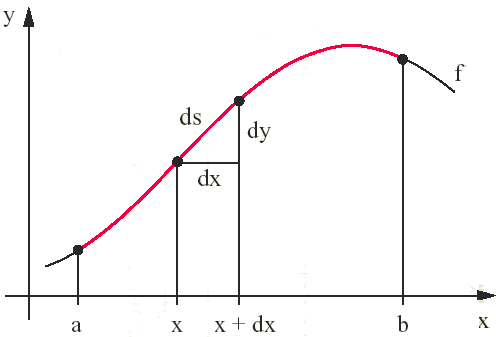
\includegraphics[width=\textwidth]{../Mathematik_2/Bilder/integration_bogenlaenge_bogenelement.png}
\end{minipage}
	\begin{minipage}{0.7\textwidth}
	Es sei $f: [a,b]\to \mathbb R$ eine differenzierbare Funktion.
			Das Integral
\[
	L = \int\limits_{a}^{b} \sqrt{1+\left( f'(x)\right)^2 }\, \mathrm{d}x
\]
		ist die L�nge des Graphen von \(f\) f�r \(x\in [a,b]\)
		\vspace{0.2cm}

		\noindent Bemerkungen:
		\begin{itemize}
	\item Das Integral nennt man ein Bogenintegral.
	\item Anstatt L�nge des Graphens sagt man Bogenl�nge.
	\item \(f\) nennt man eine Parametrisierung des Bogens.
		\end{itemize}
\end{minipage}
\end{defbox}

\begin{exabox}{Bogenl�nge}{ }
	Parametrisierung:
	\[
		f: [0,1] \to \mathbb R, x\mapsto x^2
	\]
	Ableitung:
	\[
	f'(x) = 2\cdot x
	\]
	Bogenl�nge:
	\begin{eqnarray*}
		L = \int_{0}^1 \sqrt{1 + 2\cdot x} \, \mathrm{d}x = \frac12\cdot \int\limits_1^3 \sqrt{\tilde x }\,\mathrm{d}\tilde x =   \frac12\cdot \frac 23 \cdot \Big[ \tilde x^{\frac32} \Big]_1^3 = \sqrt{3} - \frac13\,.
	\end{eqnarray*}
\end{exabox}

% Entsprechend kann man sich die L�nge einer Raumkurve herleiten. Es gilt:
% \begin{theorembox}{Bogenl�nge 3D}{ }
% 	Es sei die Parametrisierung einer Raumkurve $\gamma: [a,b] \to \mathbb R^3$  gegeben:
% 	\[ \gamma: [a,b]\to \mathbb R^3, t\mapsto (x(t), y(t), z(t))^\intercal\,,\]
% 	wobei $x, y, z$ differenzierbar sind. Die L�nge der Kurve ist
% \[
% 	|\gamma| = \int\limits_{a}^{b} \|\gamma'(t)\| \mathrm{d} t = \int\limits_{a}^b \sqrt{ (x'(t))^2 + (y'(t))^2 + (z'(t))^2}\,\mathrm{d}t \,,
% \]
% wobei $\gamma'(t) = \left( x'(t), y'(t), z'(t)\right)^\intercal$.
% \end{theorembox}
%
% \begin{exabox}{Bogenl�nge 3D}{ }
% 	Parametrisierung:
% 	\[
% 		\gamma: [0,1] \to \mathbb R^3, t\mapsto \left(\sqrt{2} t, e^t, 1-e^{-t}\right)^\intercal
% 	\]
% 	Ableitung (Geschwindigkeitsfeld):
% 	\[
% 		\gamma'(t) = (\sqrt{2}, e^t, e^{-t})^\intercal
% 	\]
% 	L�nge der Raumkurve:
% 	\begin{eqnarray*}
% 		|\gamma| &=& \int_{0}^1 \sqrt{2 + e^{2t} + e^{-2t}} \, \mathrm{d}t = \int\limits_0^1 \sqrt{ 2 + \left( e^{t} + e^{-t}\right)^2 - 2 e^{t}e^{-t} }\,\mathrm{d}t = \int\limits_0^1   \left( e^{t} + e^{-t}\right) \,\mathrm{d}t \\
% 		& =&  \Big[ e^t - e^{-t}\Big]_0^1 = e-1 - \frac1e +1 = e - \frac1e\,.
% 	\end{eqnarray*}
% \end{exabox}


 \newpage % 06 Anwendungen der Integration: Energie Mittelwert

\chapter{Funktionenr�ume und Projektion}
\section*{Leitidee}
Bisher haben wir Funktionen vor allem als einzelne Rechenvorschriften betrachtet.  Nun gehen wir einen Schritt weiter: Wir fassen Funktionen selbst als Elemente eines Raumes auf. Funktionen lassen sich addieren und mit Zahlen multiplizieren und bilden damit � ganz analog zu Vektoren � eine lineare Struktur.

Dadurch wird es m�glich, Methoden der linearen Algebra auf Funktionen anzuwenden. Insbesondere k�nnen wir mit Hilfe eines geeigneten Skalarprodukts Begriffe wie L�nge, Abstand und Orthogonalit�t auch f�r Funktionen definieren.

In technischen Anwendungen ist es h�ufig notwendig, eine Funktion m�glichst gut durch einfachere Funktionen zu approximieren.  Die Orthogonalprojektion liefert daf�r ein systematisches Verfahren: Eine Funktion wird auf einen geeigneten Unterraum projiziert und dort durch diejenige Funktion ersetzt, die den kleinsten Abstand besitzt.

Dieses Prinzip der Projektion bildet die Grundlage f�r viele sp�tere Methoden, insbesondere f�r die Fourieranalyse, bei der Funktionen als �berlagerung harmonischer Schwingungen dargestellt werden.

\bigskip
\etocsettocstyle{\section*{Inhalt dieses Kapitels}}{}
\localtableofcontents
\newpage

\setcounter{def}{0} \setcounter{satz}{0} \setcounter{exa}{0} \section{Integrierbare Funktionen}\label{MA2-integrierbare-funktionen}

\begin{table}[H]
  \centering
  \begin{tabularx}{\textwidth}{@{}>{\raggedright\arraybackslash}X r@{}}
    \toprule
    \multicolumn{2}{c}{\textbf{�bersicht �ber Lernziele und Voraussetzungen}}\\
    \midrule
    \textbf{Lernziele} & \\[.5\normalbaselineskip]
    \tabitem ein Skalarprodukt im Funktionenraum definieren und zur Rechnung verwenden & \\
    \tabitem die Norm einer Funktion aus dem Skalarprodukt bestimmen und Funktionen normieren & \\
    \tabitem Orthogonalit�t von Funktionen durch Berechnung des Skalarprodukts pr�fen & \\
    \tabitem den Begriff \emph{Orthonormalsystem} f�r Funktionen formulieren und anwenden & \\
    \tabitem die Orthonormalit�t von Funktionenpaaren bzgl eines Skalarprodukts pr�fen & \\[.5\normalbaselineskip]
    \midrule
    \textbf{Voraussetzungen} & \\[.5\normalbaselineskip]
    \tabitem mit Skalarprodukten und Normen in $\mathbb R^n$ umgehen k�nnen & \abschnittsverweis{MA1-vektoren} \\
    \tabitem Integrale berechnen k�nnen & \abschnittsverweis{MA2-integrationsregeln}\\
    \tabitem trigonometrische Funktionen sicher anwenden k�nnen & \abschnittsverweis{MA1-verkettung-von-funktionen} \\
    \bottomrule
  \end{tabularx}
\end{table}

\noindent \ifintegriereaufgaben Die �bungsaufgaben zum Thema finden Sie \hyperref[MA2-integrierbare-funktionen-aufgaben]{hier}.
\vspace{0.3cm}
\hrule
\fi


\subsection{Vom $\mathbb{R}^n$ zum Funktionenraum}

Im $\mathbb{R}^n$ haben wir das \underline{Skalarprodukt}\randverweis{MA1-vektoren}  kennengelernt, es war wie folgt definiert

\[
	\forall \, \vec x, \vec y \in \mathbb R^n: \quad \langle \vec x,\vec y\rangle = \sum_{i=1}^n x_i \cdot  y_i\,.
\]

Analog definieren wir f�r zwei Funktionen \(f, g\), die �ber dem Intervall $[a,b]$ integrierbar sind\footnote{Stetigkeit auf \((a,b)\) und Beschr�nktheit auf \([a,b]\) garantiert beispielsweise die Integrierbarkeit}:

\[
	\langle f,g\rangle = \int\limits_a^b f(x)\cdot g(x)\,\mathrm d x\, .
\]
Und das ist sinnvoll, denn offensichtlich gilt (genauso wie f�r Spaltenvektoren)
\[
	\langle f,f \rangle = \int\limits_a^b f(x)^2 \,\mathrm d x \geq 0 \, .
\]

Tats�chlich gibt es wenig Unterschied in der Art und Weise wie wir Vektoren miteinander verarbeiten und derjenigen wie wir Funktionen miteinander verarbeiten:
\begin{itemize}
	\item Addition klappt,

\[ f,g \; \quad \textnormal{Funktionen } \Rightarrow f+g \; \quad \textnormal{auch wieder eine Funktion}\,,\]

\item Skalierung klappt
\[ \lambda \textnormal{ Skalar }, f \; \quad \textnormal{Funktion } \Rightarrow \lambda \cdot f \; \quad \textnormal{auch wieder eine Funktion}\,,\]

\item und ein Skalarprodukt haben wir auch!
\end{itemize}
Es wundert einem deshalb kaum, dass wir Begriffe und Strukturen, die wir aus der linearen Algebra kennen, nun wieder auftauchen und zwar zur Analyse von Mengen von Funktionen. Funktionen sind tats�chlich Vektoren, Vektoren in einem unendlichdimensionalen Raum.

Einen Vektor \(\vec x \in \mathbb R^n\) haben wir normiert, in dem wir ihn durch seine L�nge (Norm) geteilt haben, also
\[ \hat  x := \dfrac{\vec x}{\| \vec x\|}\,, \quad \textnormal{ wobei } \;  \| \vec x\| = \sqrt{ \langle \vec x, \vec x \rangle } \,. \]
Und entsprechend l�sst sich aus einer Funktion \(f\) abstrakt dessen normiertes Gegenst�ck defninieren:
\[ \hat  f := \dfrac{f}{\| f\|}\,, \quad \textnormal{ wobei } \;  \| f\| = \sqrt{ \langle f, f \rangle } \,. \]
\begin{itemize}
	\item Das Symbol \(\| f\|\) nennen wir die Norm der Funktion \(f\). Den Begriff L�nge nuzt man f�r Funktionen nicht.
	\item Zur Berechnung von \(\| f\|\) m�ssen wir wissen, wie das Skalarprodukt definiert ist - genauer die Integrationsgrenzen \(a,b\) m�ssen festgelegt sein.
\end{itemize}

\begin{exabox}{Normierung einer Funktion}{ }
	Skalarprodukt:
\[
	\langle f,g \rangle = \int\limits_{-1}^{1} f(x)\cdot g(x) \,\mathrm d x
\]

	Funktion:
	\[ p_1: [-1,1]\to \mathbb R, x \mapsto x \]
		Norm:
		\[ \| p_1 \|^2 = \int\limits_{-1}^1 p_1(x)^2 \, \mathrm d x = \int\limits_{-1}^1 x^2 \, \mathrm d x = \Big[ \frac13 x^3\Big]_{-1}^1= \frac23 \Rightarrow \|p_1\| = \sqrt{\frac23} \,.\]
		Normierung:
		\[ \hat p_1 (x) = \frac{1}{ \|p_1\|} \cdot p_1(x) = \frac{1}{\sqrt{\frac23}} \cdot x = \frac32 \cdot x\,.\]
\end{exabox}


\subsection{Orthogonalit�t von Funktionen}

Das Skalarprodukt ist so wertvoll, weil es Orthognoalit�t definiert: zwei Funktionen hei�en \textbf{orthogonal}, wenn

\[
\langle f,g\rangle = 0 \; \Rightarrow \; f\perp g \,.
\]

Wir schauen uns jetzt Beispiele f�r Funktionenp�rchen und Skalarprodukte an und pr�fen, ob die Funktionen orthogonal sind.

\begin{exabox}{Orthogonale Funktionen}{ }
	Funktionen:
	\[\begin{cases}  f: & [-1,1]\to \mathbb R, x \mapsto 1  \\  g: & [-1,1]\to \mathbb R, x \mapsto x \end{cases}\]
		Skalarprodukt:
		\[ \langle f, g \rangle  = \int\limits_{-1}^1 f(x) \cdot g(x) \, \mathrm d x = \int\limits_{-1}^1 1\cdot x \, \mathrm d x = \Big[ \frac12 x^2\Big]_{-1}^1= \frac12\cdot (1^2- (-1)^2) = 0\]
		Schlussfolgerung: \(f \perp g\)
\end{exabox}


\begin{exabox}{Orthogonale Funktionen}{ }
	Funktionen:
	\[\begin{cases}  f: & [-1,1]\to \mathbb R, x \mapsto 1  \\  g: & [-1,1]\to \mathbb R, x \mapsto x^2 \end{cases}\]
		Skalarprodukt:
	\[ \langle f,  g \rangle  = \int\limits_{-1}^1 f(x) \cdot g(x) \, \mathrm d x = \int\limits_{-1}^1 1\cdot x^2 \, \mathrm d x = \Big[ \frac13 x^3\Big]_{-1}^1= \frac13\cdot (1)^3 - (-1)^3) = \frac23\]
		Schlussfolgerung: \(f\not \perp g\)
\end{exabox}

Monome sind also im Allgemeinen nicht paarweise orthogonal! Und noch ein Beispiel mit harmonischen Schwingungen an - beachte, dass das Integrationsgebiet in diesem Skalarprodukt das Intervall \( [-\pi, \pi]\) ist.

\begin{exabox}{Orthogonale Funktionen}{ }
	Funktionen \(f, g\):
	\[\begin{cases}  f: & [-\pi,\pi]\to \mathbb R, x \mapsto \sin(x)  \\  g: & [-\pi,\pi]\to \mathbb R, x \mapsto \cos(x) \end{cases}\]
		Skalarprodukt:
		\[ \langle f,  g \rangle  = \int\limits_{-\pi}^\pi \sin(x) \cdot \cos(x) \, \mathrm d x = \Big[ \frac12 \sin(x)^2\Big]_{-\pi}^\pi= \frac12\cdot (0- 0) = 0\]
		Schlussfolgerung: \(f \perp g\)
\end{exabox}

Interessanterweise kann man zeigen, dass alle harmonischen Schwingungen der Form \[ s_n: x\mapsto \sin(n\cdot x), \quad n \in \mathbb N^+ \] und \[ c_m: x\mapsto \cos(m\cdot x), \quad m \in \mathbb N_0 \]  �ber \([-\pi,\pi]\) \textbf{paarweise orthogonal} sind. Auf mathematisch gilt also folgendes

\[
	\langle s_n, c_m \rangle = \int\limits_{-\pi}^\pi \sin(n\cdot x) \cdot \cos(m\cdot x)\,\mathrm d x  = 0\,.
\]

Und das ist nicht genug, es gilt auch:

\[
	\begin{array}{rcl}
		\langle s_n, s_m \rangle &=& \displaystyle \int\limits_{-\pi}^\pi \sin(n\cdot x) \cdot \sin(m\cdot x)\,\mathrm d x  = 0, \quad n\not=m\,, \\[2ex]
	\langle c_n, c_m \rangle &=& \displaystyle \int\limits_{-\pi}^\pi \cos(n\cdot x) \cdot \cos(m\cdot x)\,\mathrm d x  = 0, \quad n\not=m\,. \end{array}
\]

Die Funktionen
\[
	\left\{ 1, \sin(n\cdot x), \cos(n\cdot x), \quad n \in \mathbb N\right\}
\]
sind bez�glich des Skalarprodukts
\[
\langle f,g\rangle
=
\int\limits_{-\pi}^{\pi} f(x)\cdot g(x)\,\mathrm dx
\]
orthogonal.

\subsection{Orthonormalsystem}

Eine Menge von Funktionen hei�t \emph{Orthogonalsystem}, wenn die Funktionen normiert und paarweise orthogonal zueinander sind.
Mit dem Skalarprodukt
\begin{equation}\label{skp_orthonormalsystem}
\langle u,v\rangle
=
\frac{1}{\pi}
\int_{1}^{2\pi} u(t)\cdot v(t)\,\mathrm dt
\end{equation}
werden die harmonischen Schwingungen aus dem vorigen Abschnitt automatisch normiert. Wir kennen also ein konkretes Beispiel f�r ein Orthogonalsystem.

Um orthographisch kenntlich zu machen, dass wir die harmonischen Schwingungen ab jetzt immer mit dem Skalarprodukt betrachen, in dem sie ein Orthonormalsystem bilden, nutzen den kleinen Hut:

\[ \left\{ \begin{array}{rcl l} \hat s_n(t): &=& \sin(n\cdot t)\,, &\quad n\geq 1\,, \\  \hat c_n(t): &=& \cos(n\cdot t)\,, & \quad n\geq 1 \,.\end{array}\right.  \]

\begin{exabox}{Orthonormalsystem}{ }
	Die Funktionen
\[
	M = \left\{ 1, \hat s_n, \hat c_n, \; n \in \mathbb N\right\}
\]
bilden bez�glich \eqref{skp_orthonormalsystem} ein Orthonormalsystem und das hei�t, dass f�r alle \(n,m\in \mathbb N^+\) gilt
\[
	\begin{array}{rl}
		\textnormal{paarweise orthogonal:} & \quad \left\{
	\begin{array}{rcl l}
		\langle 1, \hat c_n\rangle &=& 0 & \\
		\langle 1, \hat s_n\rangle &=& 0 & \\
		\langle \hat c_n, \hat s_m\rangle &=& 0\,, &  \\
		\langle \hat c_n, \hat c_m\rangle &=& 0\,, & n\not=m \\
		\langle \hat s_n, \hat s_m\rangle &=& 0\,, & n\not=m \\
\end{array} \right. \\
		\textnormal{normiert} & \quad \left\{
	\begin{array}{rcl}
		\langle 1, 1\rangle &=& 1\\
		\langle \hat s_n, \hat s_n\rangle &=& 1\\
		\langle \hat c_n, \hat c_n\rangle &=& 1
\end{array} \right.
\end{array}
\]

\end{exabox}

Das Orthonormalsystem $M$ besitzt zwei zentrale Eigenschaften:

\begin{itemize}
  \item Alle Funktionen sind $2\pi$-periodisch.
  \item Linearkombinationen bleiben ebenfalls $2\pi$-periodisch.
\end{itemize}

Die gemeinsame Periode ist entscheidend:
�berlagert man zwei Funktionen aus $M$,
so entsteht wieder eine $2\pi$-periodische Funktion.
Dasselbe gilt f�r jedes skalare Vielfache.

Damit verh�lt sich $M$ strukturell wie eine Basis im
endlichdimensionalen Vektorraum �
nur dass wir uns hier in einem Funktionenraum befinden.

In der Fourier-Analyse werden wir dieses Orthonormalsystem
verwenden, um $2\pi$-periodische Funktionen als
Reihenentwicklungen in harmonischen Schwingungen darzustellen.

 \newpage % 07 Integrierbare Funktionen
%\setcounter{exercise}{0} 
\ifintegriereaufgaben

\section*{Integrierbare Funktionen Aufgaben}\label{MA2-integrierbare-funktionen-aufgaben}
Erkl�rungen und Beispiele, die zur Bearbeitung der Aufgaben hilfreich sind, finden Sie im Skript\wennreferenzvorhanden{MA2-integrierbare-funktionen}{ (Abschnitt \abschnittsverweis{MA2-integrierbare-funktionen})} und, falls Sie nicht weiterkommen, schauen Sie \hyperref[MA2-integrierbare-funktionen-loesungen]{hier}.
\else
\section{Integrierbare Funktionen Aufgaben}\label{MA2-integrierbare-funktionen-aufgaben}

Regeln und Beispiele zu diesen Aufgaben finden Sie im Skript. Die L�sungen finden Sie \hyperref[MA2-integrierbare-funktionen-loesungen]{hier}.
\fi

\begin{exercisebox}[Gram-Schmidtsches Orthogonalisierungsverfahren]
	Gegeben sind drei linear unabh�ngige Vektoren. Bestimmen Sie ein Orthonormalsystem.
	\[
		\boldsymbol v_1 = \left( \begin{array}{c} 1 \\ i \\ 0 \\ 0 \end{array}\right)\,,
		\boldsymbol v_2 = \left( \begin{array}{c} i \\ 0 \\ 0 \\ i \end{array}\right)\,,
		\boldsymbol v_3 = \left( \begin{array}{c} 1 \\ 0 \\ 1 \\ 0 \end{array}\right)\,.
	\]
\end{exercisebox}

\begin{exercisebox}[Basis] %https://www.lntwww.de/Aufgaben:Aufgabe_4.1:_Zum_Gram-Schmidt-Verfahren
	Bei der Digitalsignal�bertragung werden energiebegrenzte Signale betrachtet. Das Skalarprodukt zweier Signale bzw. die Norm eines Signals sind hierbei wie folgt definiert:
	\begin{eqnarray*}
		\langle s_i, s_k\rangle &=& \int\limits_{-\infty}^{\infty} s_i(t) \cdot s_k(t) \, \mathrm{d}t\,,\\[1ex]
		\|s\| &=& \sqrt{\langle s,s \rangle}\,.
	\end{eqnarray*}
	Betrachten Sie die folgenden drei energiebegrenzten Signale:
	\begin{center}
	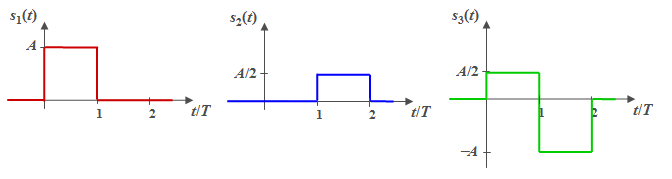
\includegraphics[width=0.7\textwidth]{../Mathematik_2/Bilder/funktionenraum_rechtecksignale_linearkombination.png}
\end{center}
	\begin{itemize}
		\item[(a)] Wie lauten die Abbildungsvorschriften der Signale $s_1, s_2$ und $s_3$?
		\item[(b)] Berechnen Sie die Normen der Signale $s_1$ und $s_2$.
		\item[(c)] Konstruieren Sie aus den Signalen $s_1$ und $s_2$ ein Orthonormalsystem.
		\item[(d)] Zerlegen Sie das Signal $s_3$ bez�glich des Orthonormalsystems und bestimmen Sie die vektoriellen Repr�sentanten der Ausgangssignale bez�glich des Orthonormalsystems.
	\end{itemize}
\end{exercisebox}

\begin{exercisebox}[Orthogonalit�tsrelationen]
	Berechnen Sie f�r alle $k,l\in\mathbb N_0$ mit $\omega = 2\pi/T$ die folgenden Integrale:
	\begin{eqnarray*}
		(a)\, \int\limits_{0}^{T} \cos(k\omega t) \cdot \cos(l\omega t)\, \mathrm{d}t\,, \quad (b)\, \int\limits_{0}^{T} \sin(k\omega t) \cdot \sin(l\omega t)\, \mathrm{d}t\,,\quad (c)\, \int\limits_{0}^{T} \cos(k\omega t) \cdot \sin(l\omega t)\, \mathrm{d}t
	\end{eqnarray*}
\end{exercisebox}


 \newpage  % Funktionen als Vektoren, Skalarprodukt
\setcounter{def}{0} \setcounter{satz}{0} \setcounter{exa}{0} \section{Fourier-Polynome und Projektion (+)}\label{MA2-fourierpolynome-und-projektion}

\begin{table}[H]
  \centering
  \begin{tabularx}{\textwidth}{@{}>{\raggedright\arraybackslash}X r@{}}
    \toprule
    \multicolumn{2}{c}{\textbf{�bersicht �ber Lernziele und Voraussetzungen}}\\
    \midrule
    \textbf{Lernziele} & \\[.5\normalbaselineskip]
    \tabitem ein Fourier-Polynom als Element eines endlichdimensionalen Unterraums interpretieren & \\
    \tabitem den Approximationsraum $U_N$ explizit beschreiben & \\
    \tabitem das Fourier-Polynom als orthogonale Projektion einer Funktion auf $U_N$ verstehen & \\
    \tabitem die Bestapproximationseigenschaft mit Hilfe des Skalarprodukts formulieren & \\
    \tabitem das Residuum als orthogonalen Fehler interpretieren & \\[.5\normalbaselineskip]
    \midrule
    \textbf{Voraussetzungen} & \\[.5\normalbaselineskip]
    \tabitem mit Orthonormalsystemen in Funktionenr�umen umgehen k�nnen & \abschnittsverweis{MA2-integrierbare-funktionen}\\
    \tabitem Skalarprodukt und Norm in Funktionenr�umen anwenden k�nnen & \abschnittsverweis{MA2-integrierbare-funktionen} \\
    \tabitem Fourier-Koeffizienten berechnen k�nnen & \abschnittsverweis{MA2-fourierreihen}  \\
    \bottomrule
  \end{tabularx}
\end{table}

\noindent \ifintegriereaufgaben Die �bungsaufgaben zum Thema finden Sie \hyperref[MA2-fourierpolynome-und-projektion-aufgaben]{hier}.
\vspace{0.3cm}
\hrule
\fi

Die Fourier-Reihe wurde als Entwicklung einer Funktion in einem Orthonormalsystem mit unendlich vielen Basisfunktionen eingef�hrt.

Liegt ein global stetiges, $T$-periodisches Signal $u$ vor, so konvergiert die Fourier-Reihe punktweise gegen $f$:

\[
u(t)
=
\frac{a_0}{2}
+
\sum_{n=1}^{\infty}
\left(
	a_n\cdot \cos(\omega_n\, t)
+
b_n \cdot \sin(\omega_n\, t)
\right)\,, \quad \omega_n = n\cdot \omega_0\,.
\]

\bigskip

\subsection*{Abbruch nach endlich vielen Harmonischen}

Bricht man die Reihenentwicklung nach $N$ Harmonischen ab, so erh�lt man ein Fourier-Polynom vom Grad $N$:

\[
u_N(t)
=
\frac{a_0}{2}
+
\sum\limits_{n=1}^{N}
\left(
	a_n \cdot \cos(\omega_n\, t)
+
b_n \cdot \sin(\omega_n\, t)
\right)\,, \quad \omega_n = n\cdot \omega_0\,.
\]

Im Allgemeinen gilt:
\[
	u_N \neq u\,.
\]

Was also ist $u_N$?  Welche Bedeutung besitzt dieses Polynom?

\subsection*{Der zugrunde liegende Unterraum}

Betrachten wir den endlichdimensionalen Raum

\[
U_N
=
\mathrm{LH}
\left\{
	1,\cos(\omega_0\, t),\sin(\omega_0\, t),\cos(\omega_1\, t),\sin(\omega_1\, t),\cos(\omega_2\, t),\sin(\omega_2\, t),
\dots,
\cos(\omega_N\, t),\sin(\omega_N\, t)
\right\} \,..
\]

Dieser Raum enth�lt die - \textbf{und nur die} - Fourier-Polynome vom Grad $N$. Er ist ein Unterraum des Funktionenraums der $T$-periodischen Funktionen. Das Fourier-Polynom $u_N$ ist ein Element dieses Raumes.

\subsection*{Beste Approximation}

Unter allen Funktionen $q \in U_N$ ist $u_N$ ausgezeichnet durch die Eigenschaft:

\[
\|u - u_N\|
=
\min_{q \in U_N}
\|u - q\|.
\]

In Worten: \(u_N\) besitzt den k�rzesten Abstand zu \(u\)! Wir sagen auch \(u_N\) ist die Bestapproximation von $u$ im Raum $U_N$ - ganz pr�zise die Bestapproximation von $u$ bez�glich der durch das Skalarprodukt induzierten Norm. Die folgende Skizze veranschaulicht die Eigenschaft von \(u_N\):
\bigskip
 \begin{center}
	 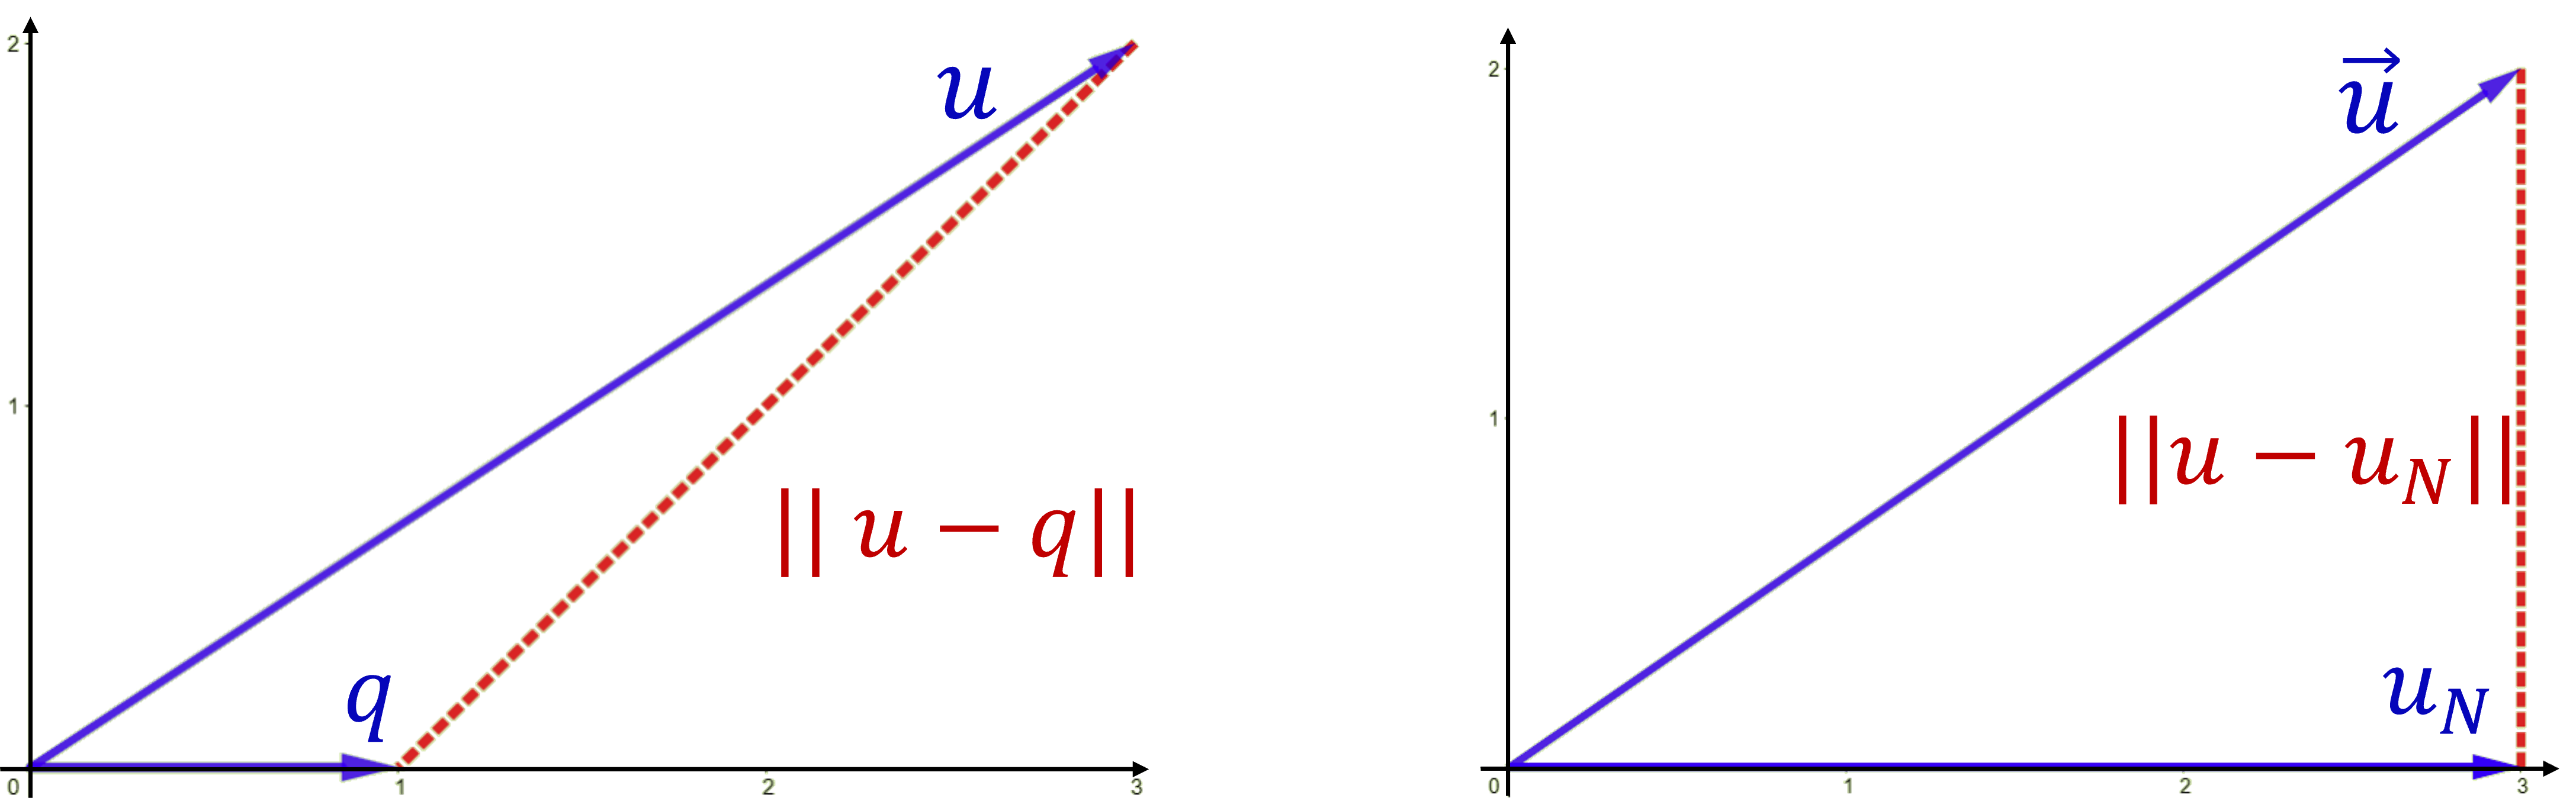
\includegraphics[width=0.7\textwidth]{../Mathematik_2/Bilder/bestapproximation_abstandsminimum_gerade.png}
 \end{center}

\subsection*{Das Residuum}

Definieren wir das sogenannte Residuum (den Abstand zwischen \(u\) und der Bestapproximation)

\[
	r := u - u_N\,.
\]

Minimal ist das Residuum genau dann, wenn es orthogonal auf dem gesamten Raum $U_N$ steht:

\[
\langle r , q \rangle = 0
\quad \text{f�r alle } q \in U_N.
\]

Insbesondere gilt f�r alle \(n \leq N\):

\[
\langle u - u_N , \hat c_n \rangle = 0,
\qquad
\langle u - u_N , \hat s_n \rangle = 0.
\]

\medskip

Das Residuum enth�lt also keine Anteile mehr in Richtung der harmonischen Schwingungen bis zur Ordnung $N$:
\[
\text{Fehler} \perp \text{Approximationsraum}.
\]

Das Fourier-Polynom $u_N$ ist die beste Approximation an die Funktion $u$ auf den Unterraum $U_N$; jedes andere Element des Raumes $U_N$ besitzt einen gr��eren Abstand zu $u$.
 \newpage % 08 Approximation im Funtionenraum
%\setcounter{exercise}{0} 
\ifintegriereaufgaben
\section*{Fourier-Polynome und Projektion Aufgaben}\label{MA2-fourierpolynome-und-projektion-aufgaben}

Erkl�rungen und Beispiele, die zur Bearbeitung der Aufgaben hilfreich sind, finden Sie im Skript\wennreferenzvorhanden{MA2-fourierpolynome-und-projektion}{ (Abschnitt \abschnittsverweis{MA2-fourierpolynome-und-projektion})} und, falls Sie nicht weiterkommen, schauen Sie \hyperref[MA2-fourierpolynome-und-projektion-loesungen]{hier}.
\else
\section{Fourier-Polynome und Projektion Aufgaben}\label{MA2-fourierpolynome-und-projektion-aufgaben}

Regeln und Beispiele zu diesen Aufgaben finden Sie im Skript. Die L�sungen finden Sie \hyperref[MA2-fourierpolynome-und-projektion-loesungen]{hier}.
\fi


\begin{exercisebox}[Bestapproximation] %A.Z. Anwendungen
	Gegeben seien die Funktionen $f_1, f_2, f_3 \in \mathcal C([-\pi,\pi], \mathbb R)$ mit
	\[ f_1: x\mapsto 1, \quad f_2: x\mapsto \cos(x), \quad f_3: x\mapsto \sin(x)\]
	\begin{itemize}
		\item[(a)] Zeigen Sie, dass die Funktionen paarweise orthogonal sind bez�glich des Skalarprodukts
			\[ \langle f, g\rangle : = \int_{-\pi}^{\pi} f(x) \cdot g(x) \, \mathrm{d}x \]
		\item[(b)] Berechnen Sie die Bestapproximation $\tilde f \in \mathcal C([-\pi,\pi],\mathbb R)$ von $f:x\mapsto x^2$ bez�glich $f_i$, $i=1,2,3$ und zeichnen Sie $f$ und $\tilde f$.
		\item[(c)] Zeigen Sie, dass die folgenden Funktionen orthogonal sind\[ \cos(k\cdot x), \, k\in \mathbb N_0, \quad \sin(k\cdot x),  \, k\in \mathbb N\,.\]
	\end{itemize}
\end{exercisebox}

\begin{exercisebox}[Bestapproximation]
	Wir betrachten \(\mathcal C([-2,2],\mathbb R)$, den Vektorraum der auf \([-2,2]\) stetigen Funktionen, ausgestattet mit der Maximumsnorm.  Zeigen Sie, dass sich $p$ nicht beliebig genau durch die Funktionen
		\[ f_1(x)=1, \quad f_2(x) = e^x,\quad f_3(x)=e^{2x} \]
		approximieren l��t.
\end{exercisebox}
 \newpage  % Bestapproximation
\setcounter{def}{0} \setcounter{satz}{0} \setcounter{exa}{0} \section{Orthogonalprojektion im $\mathbb{R}^n$ (+)}\label{MA2-orthogonalprojektion}

\begin{table}[H]
  \centering
  \begin{tabularx}{\textwidth}{@{}>{\raggedright\arraybackslash}X r@{}}
    \toprule
    \multicolumn{2}{c}{\textbf{�bersicht �ber Lernziele und Voraussetzungen}}\\
    \midrule
    \textbf{Lernziele} & \\[.5\normalbaselineskip]
    \tabitem das Prinzip �Minimalabstand $\Leftrightarrow$ Orthogonalit�t� geometrisch erkl�ren & \\
    \tabitem die Orthogonalprojektion eines Vektors auf einen Unterraum interpretieren & \\
    \tabitem ein �berbestimmtes lineares Gleichungssystem als Approximationsproblem formulieren & \\
    \tabitem die Normalengleichung $A^\top A\,\vec x = A^\top \vec b$ herleiten und anwenden & \\
    \tabitem das Residuum als orthogonalen Fehlervektor im Bildraum von $A$ deuten & \\[.5\normalbaselineskip]
    \midrule
    \textbf{Voraussetzungen} & \\[.5\normalbaselineskip]
    \tabitem Rang und Bildraum einer Matrix bestimmen k�nnen & \abschnittsverweis{MA1-lineare-gleichungssysteme}  \\
    \tabitem mit Skalarprodukten und Normen im $\mathbb R^n$ umgehen k�nnen &  \abschnittsverweis{MA1-vektoren} \\
    \tabitem Matrizen transponieren und Matrix-Vektor-Produkte berechnen k�nnen & \abschnittsverweis{MA1-matrizen}\\
    \bottomrule
  \end{tabularx}
\end{table}

\noindent \ifintegriereaufgaben Die �bungsaufgaben zum Thema finden Sie \hyperref[MA2-orthogonalprojektion-aufgaben]{hier}.
\vspace{0.3cm}
\hrule
\fi


Die bei der Fourier-Approximation beobachtete Struktur ist kein Spezialph�nomen des Funktionenraums.

Sie tritt immer dann auf, wenn ein Element eines Vektorraums durch Elemente eines Unterraums m�glichst gut approximiert werden soll.

Die zugrunde liegende Idee lautet:

\[
\text{Abstand minimiert}
\quad \Longleftrightarrow \quad
\text{Orthogonalit�tsrelation erf�llt} \,.
\]


Diese Struktur gilt in jedem Raum mit Skalarprodukt - insbesondere also auch im endlichdimensionalen Raum $\mathbb{R}^n$.

Gegeben sei ein Unterraum $V \subset \mathbb{R}^n$ und ein Vektor $\vec b \in \mathbb{R}^n$. Gesucht ist derjenige Vektor $\vec v \in V$ mit

\[
	\|\vec b - \vec v\| = \min_{\vec u \in V} \|\vec b - \vec u\|\,.
\]

Wie im Funktionenraum gilt:

\[
	\vec b - \vec v \perp V\,.
\]

\begin{exabox}{Geometrische Interpretation}{}
\begin{minipage}{0.3\textwidth}
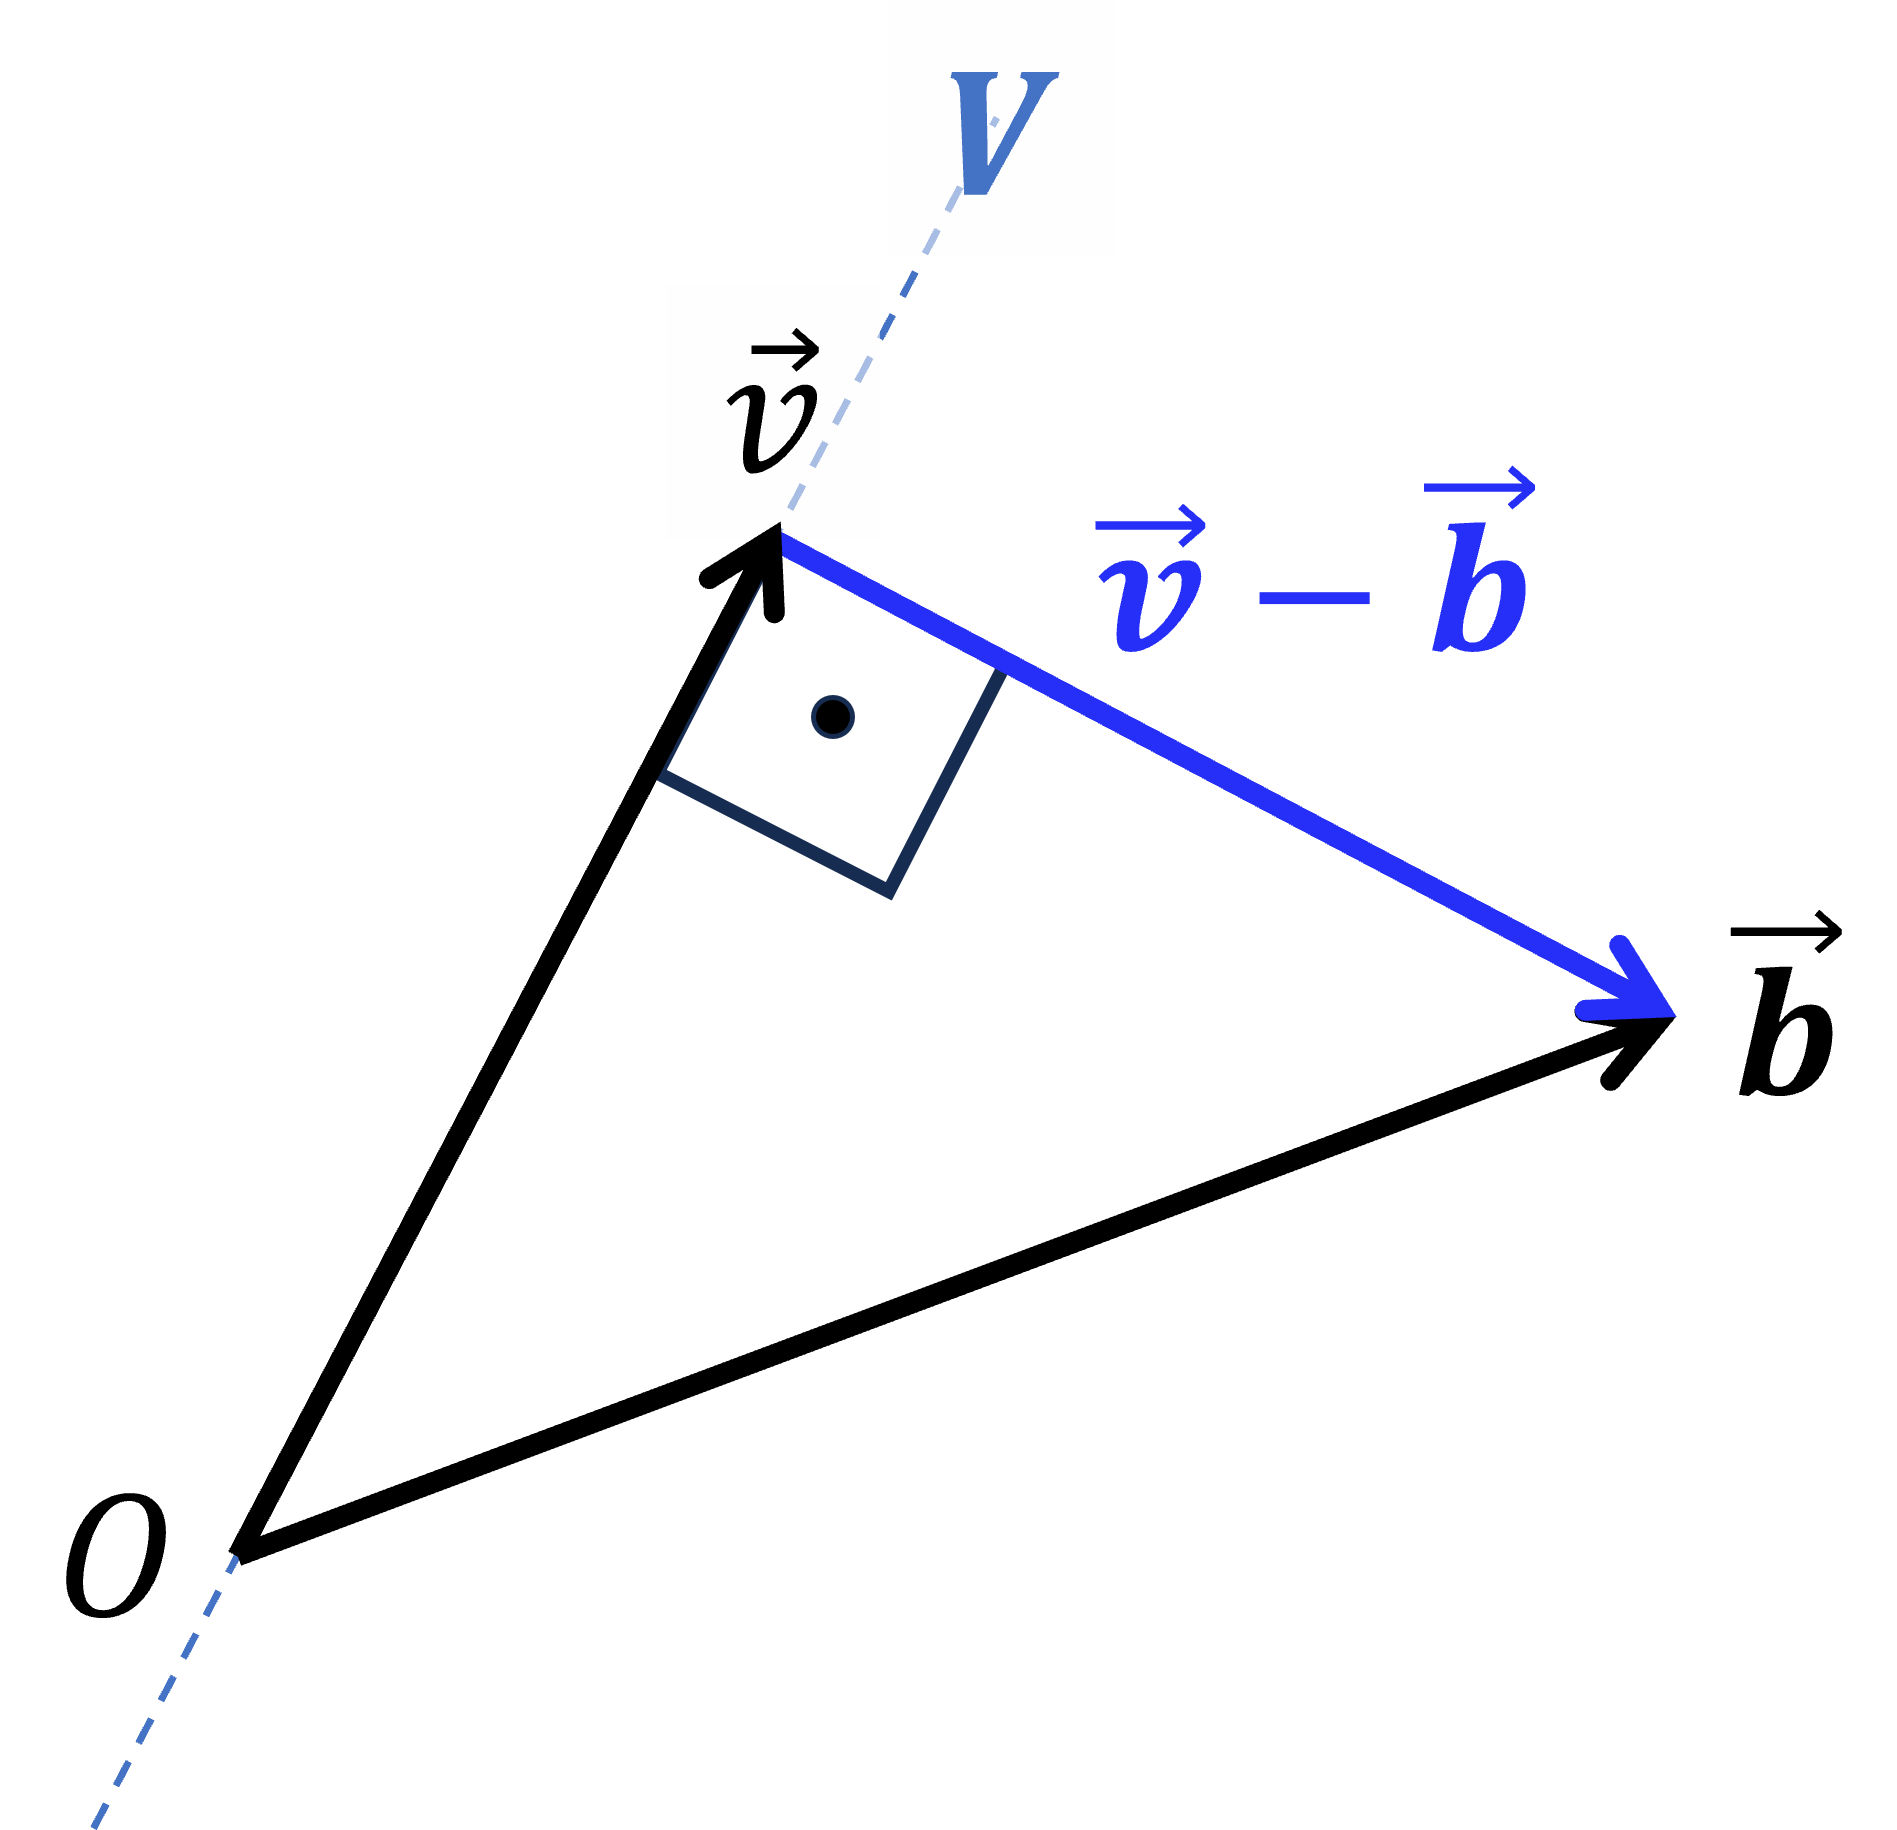
\includegraphics[width=\textwidth]{../Mathematik_2/Bilder/orthogonalprojektion_geometrie_des_residuums.png}
\end{minipage}
\begin{minipage}{0.7\textwidth}
	\begin{itemize}
		\item Das Residuum (der Fehler- oder Abstandsvektor)  \(\vec b - \vec v\) steht senkrecht auf dem gesamten Unterraum.
		\item Die Orthogonalit�t des Residuums charakterisiert den Punkt minimalen Abstands:
	\end{itemize}
\end{minipage}
\end{exabox}

\subsection*{Anwendung: L�sung eines �berbestimmten Gleichungssystems}

Betrachten wir nun ein lineares Gleichungssystem

\[
	A \vec x = \vec b, \qquad A \in \mathbb{R}^{n \times m}, \; n>m \,.
\]

Ist das System nicht l�sbar, so liegt $\vec b$ nicht im Bildraum von $A$:

\[
	\vec b \notin \mathrm{im}(A)\,.
\]

Starten wir mit einer konkreten, sehr einfachen Aufgabe: gesucht sind Zahlen \(x_1, \,  x_2 \in \mathbb R\), die folgende Gleichungen simultan erf�llen \begin{equation}\label{Beispiel1} \begin{cases} \begin{array}{rcr c l } x_1 &&&=& 1\,, \\& & x_2 &=& 1\,, \\ x_1 &+&x_2 &=& 1\end{array} \end{cases} \Rightarrow  \quad \begin{array}{cccc}
	\left( \begin{array}{cc}
			1 & 0   \\
			0 & 1   \\
			1 & 1
\end{array}\right)& \left( \begin{array}{c}x_1 \\x_2\end{array} \right) &=&  \left( \begin{array}{c} 1 \\ 1 \\ 1 \end{array}\right) \\ \underbrace{\quad\quad\quad\quad\quad\quad}_{\displaystyle{=A}} &\underbrace{\quad\quad\quad}_{\displaystyle{=\vec x}} &&  \underbrace{\quad\quad\quad}_{\displaystyle{=\vec b}} \end{array}
\end{equation}
Um den Gau�-Algorithmus anzuwenden betrachten wir die erweitertete Koeffizientenmatrix \( A_{\vec b} = \left( A|\vec b\right)\) und bringen die Matrix zun�chst auf Trapezform:

\vspace{0.1cm}
\begin{exabox}{L�sungsversuch �berbestimmtes Gleichungssystem}{ }
	\[ \begin{array}{r c l} \textnormal{Ausgangsgleichung} & & \left( \begin{array}{cc|c}
			1 & 0   & 1 \\
			0 & 1   & 1\\
	1 & 1 & 1 \end{array}\right)\\
	\textnormal{Trapezform} & \Leftrightarrow &
\left( \begin{array}{cc|c}
		1 & 0 & 1\\
		0 & 1 & 1 \\
		0 & 0 & 1
\end{array} \right) \Rightarrow \textnormal{Aufl�sen klappt nicht!} \end{array}\]
\vspace{0.1cm}
\begin{itemize}
	\item[\(\Rightarrow\)] Die L�sbarkeitsbedingung ist nicht erf�llt: \(\mathrm{rang}(A) \not=\mathrm{rang}(A_{\vec b})\).
	\item[\(\Rightarrow\)] Das Gleichungssystem ist nicht l�sbar, die L�sungsmenge ist leer!
\end{itemize}
\end{exabox}
\bigskip


Die Vektoren $A\vec x$ bilden einen Unterraum des $\mathbb{R}^n$, den Bildraum \(\mathrm{im}(A)\). Was k�nnen wir tun? Wir suchen daher denjenigen Vektor $A\vec x_*$, der $\vec b$ am n�chsten kommt.

\begin{exabox}{Nichtl�sbares Gleichungssystem}{}
\begin{minipage}{0.3\textwidth}
	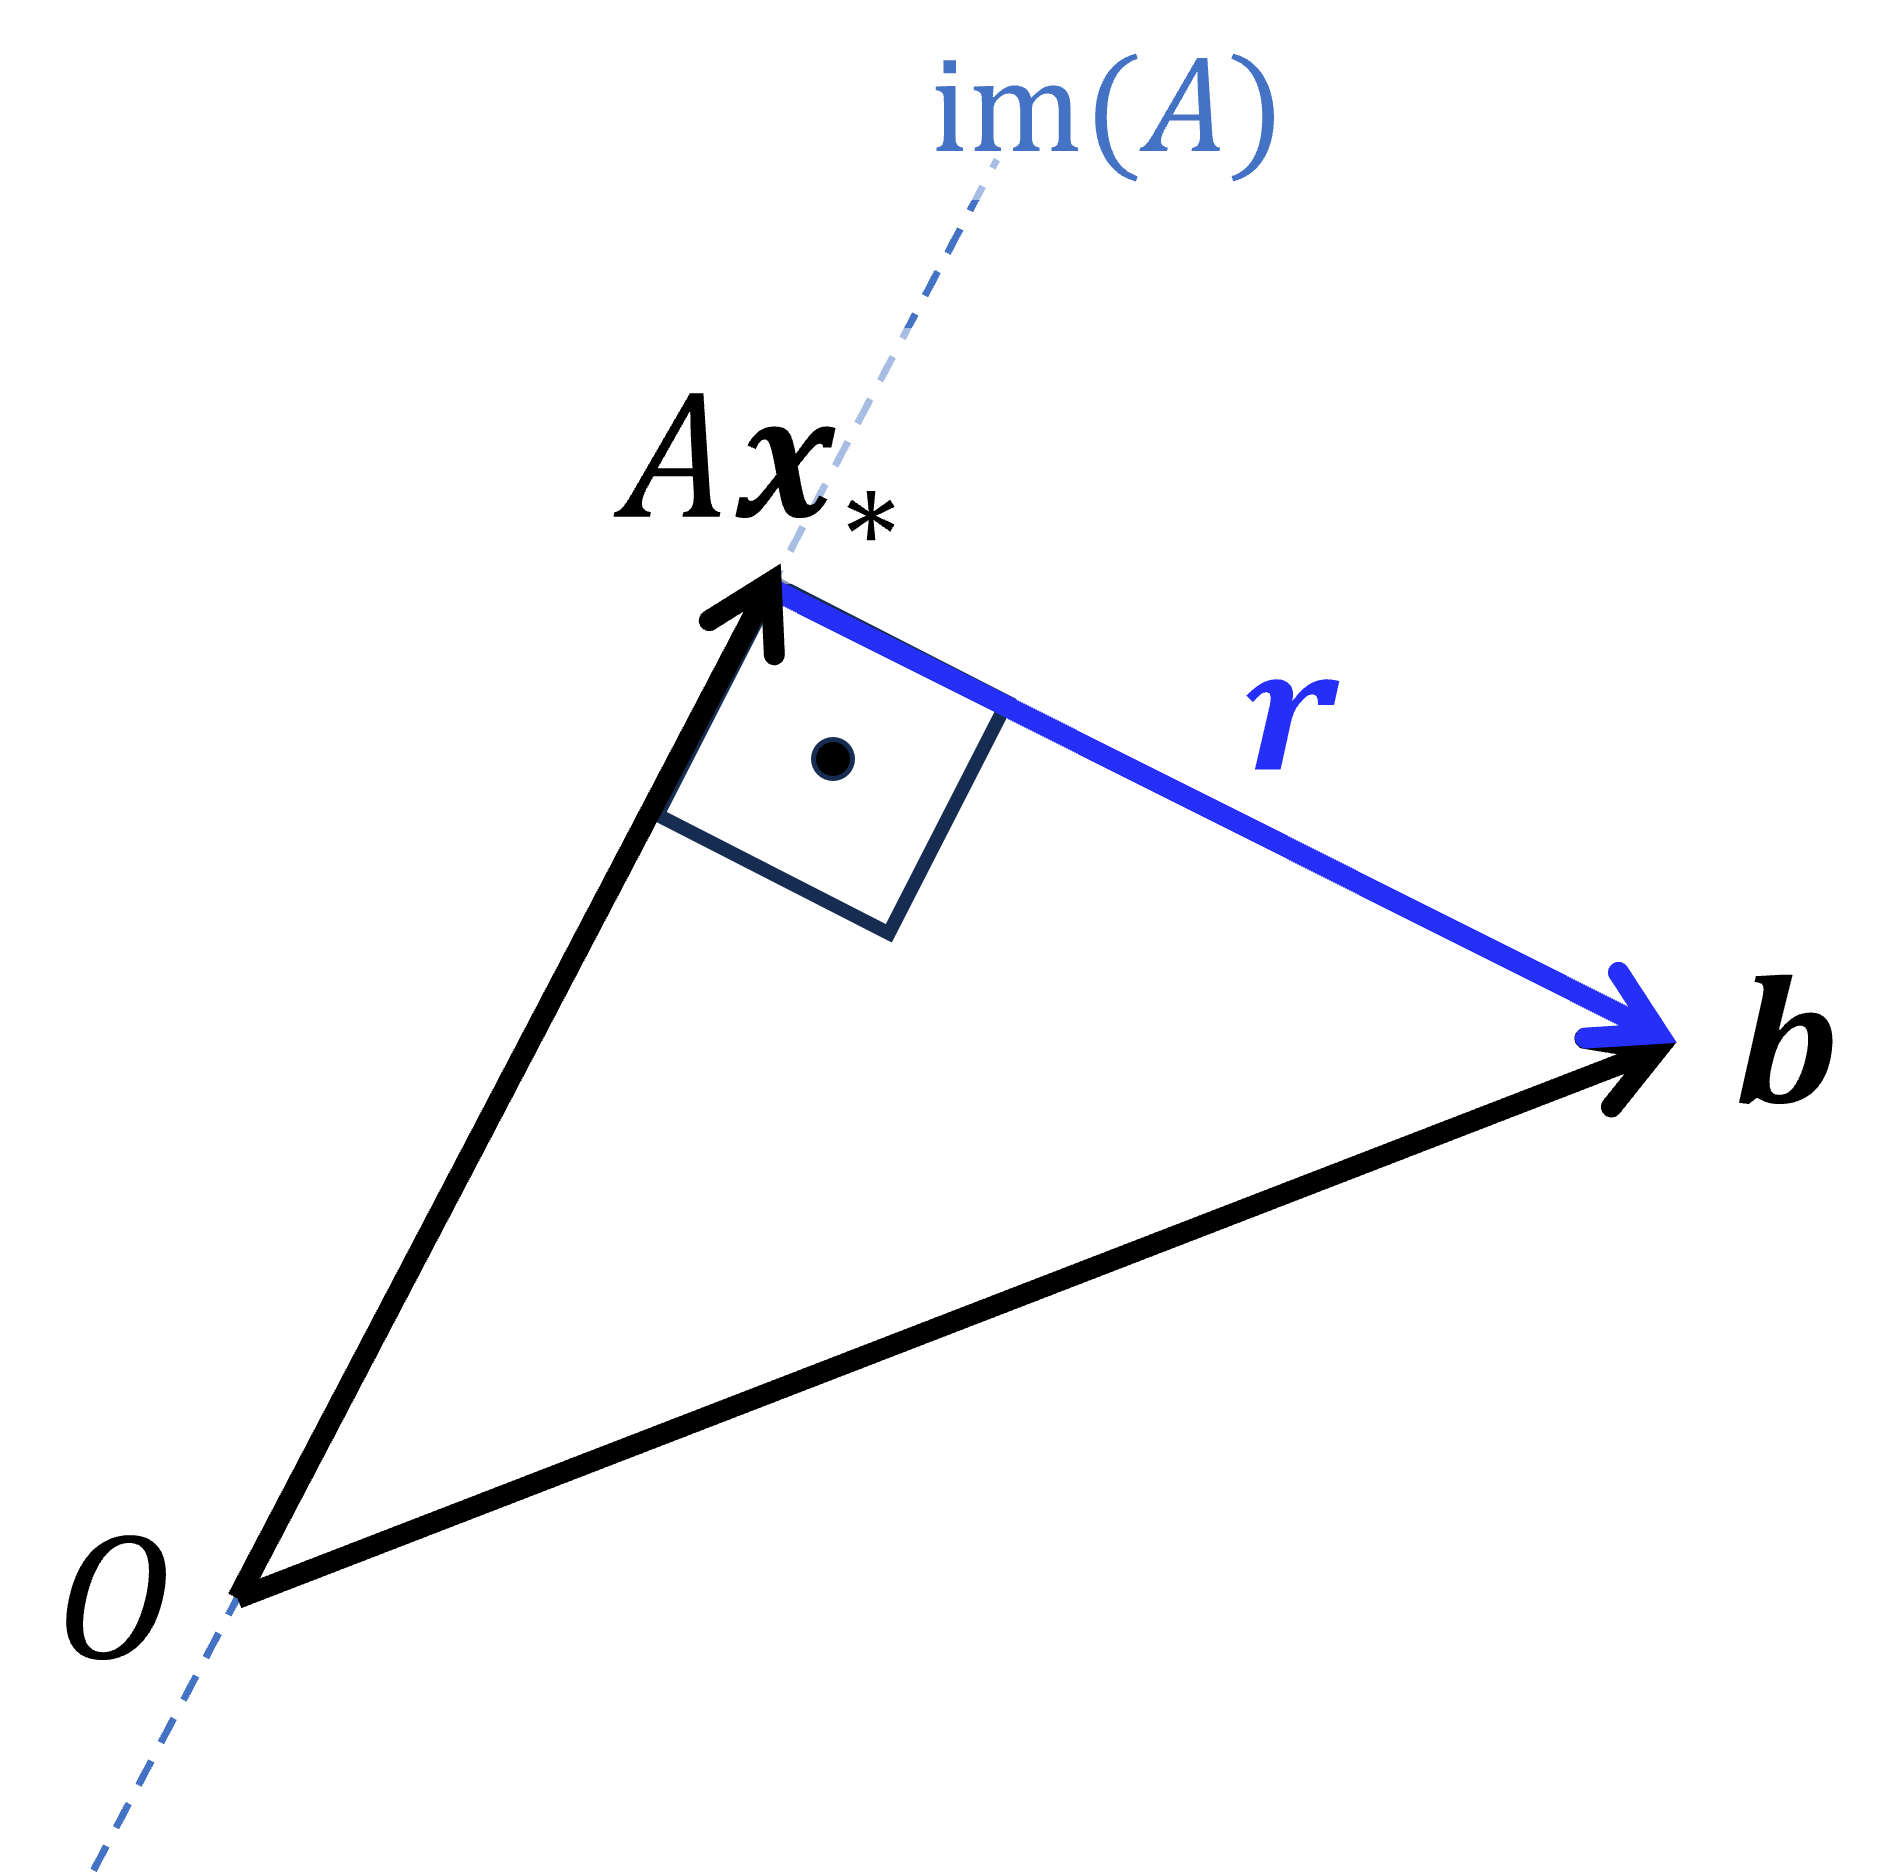
\includegraphics[width=\textwidth]{../Mathematik_2/Bilder/ausgleichsrechnung_residuum_orthogonal_zum_bildraum.png}
%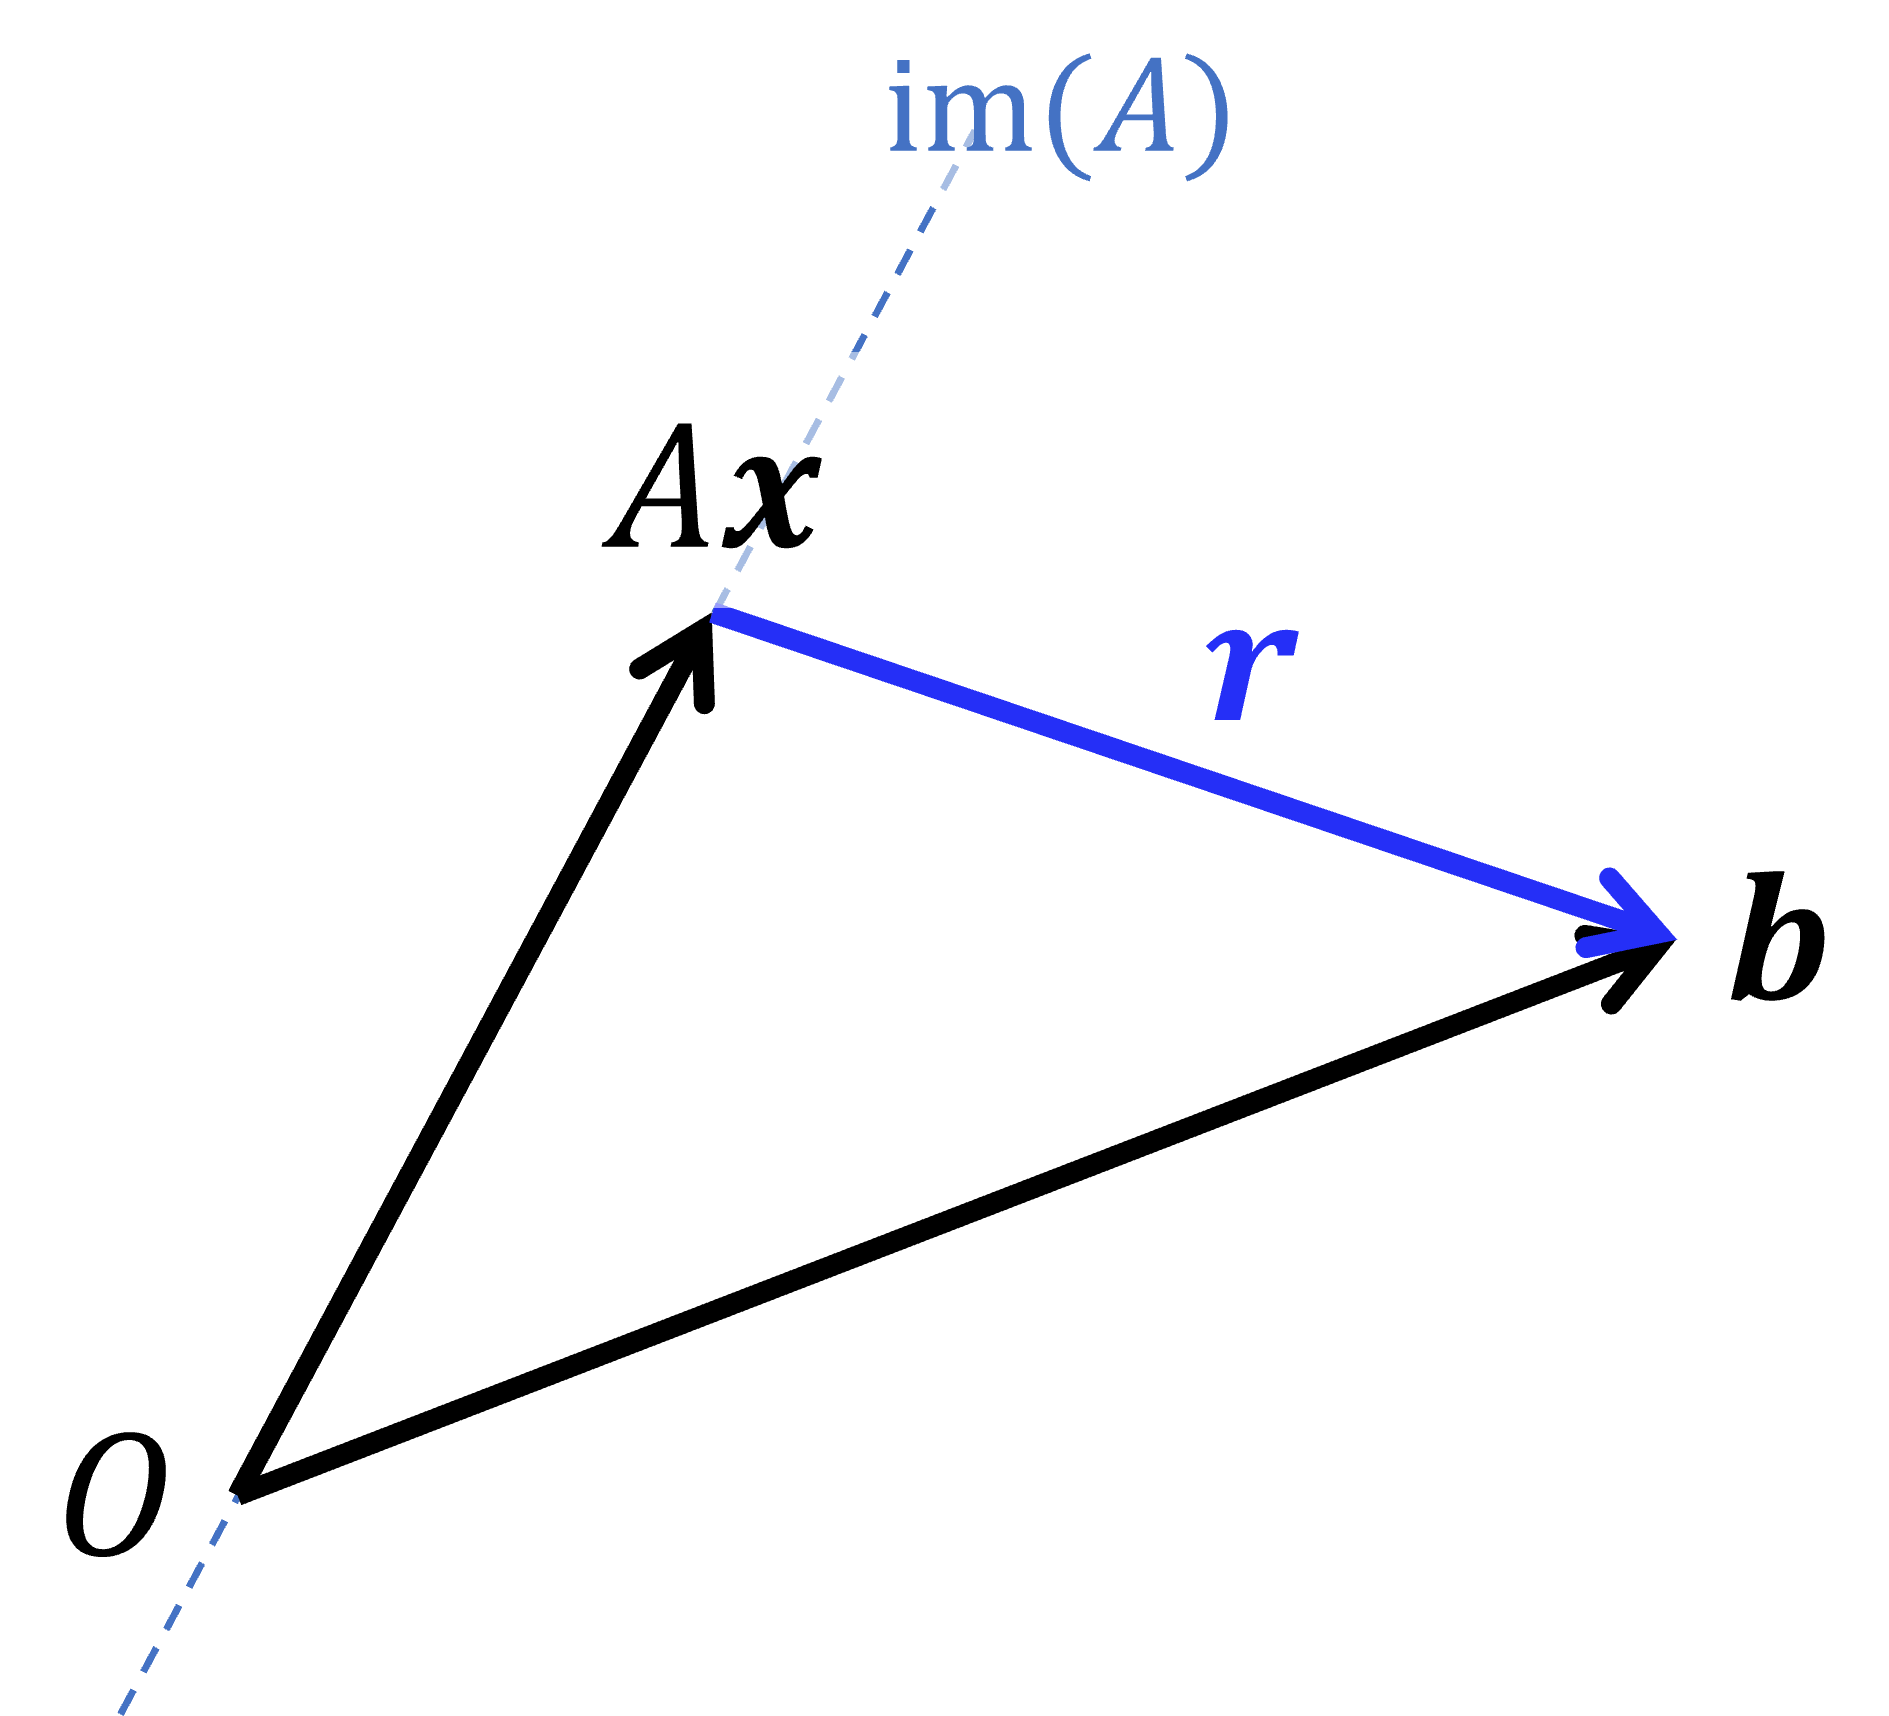
\includegraphics[width=\textwidth]{../Mathematik_2/Bilder_unused/ausgleichsrechnung_residuum_im_bildraum.png}
\end{minipage}
\begin{minipage}{0.7\textwidth}
	\begin{itemize}
		\item Ist $\vec b$ nicht im Bildraum von $A$,
existiert keine exakte L�sung.
\item Gesucht ist daher die beste Approximation im Sinne des minimalen Abstands.
	\end{itemize}
\end{minipage}
\end{exabox}
\bigskip

Wir formulieren das Minimierungsproblem:

\[
\min_{\vec x}
\|A\vec x - \vec b\|.
\]

Definiert man das Residuum

\[
	\vec r := A\vec x - \vec b\,,
\]

so gilt im Optimalfall:

\[
	\vec r \perp \mathrm{im}(A)\,.
\]

Das Element in \(\mathrm{im}(A)\), das die Orthogonalit�tsbedingung erf�llt ist die L�sung der sogenannten Normalengleichung:

\[
	A^T (A\vec x_* - \vec b) = 0\,.
\]

Die Normalengleichung ist die algebraische Formulierung der Orthogonalprojektion. Die L�sung der Normalengleichung liefert genau denjenigen Punkt im Bildraum von $A$, dessen Abstand zu $\vec b$ minimal ist. Und dass das so ist, k�nnen wir beweisen, in dem wir zeigen, dass \(\vec r \) tats�chlich orthogonal zu allen Vektoren im Bild von \(A\) ist:

\[\begin{array}{rcl l}
		\forall \, \vec x \in \mathbb R^n:\quad \langle  A\,\vec x, \vec r\rangle &=& \langle  A\,\vec x,  A\,\vec x_* - \vec b\rangle  & \| \; \textnormal{ beliebiges Element in } \mathrm{im}(A): \; A\,\vec x \\
		&=& \langle  \vec x, A^\intercal \left( A\vec x_* - \vec b \right) \rangle &\|\; \textnormal{Eigenschaft der Matrix-Vektor-Multiplikation} \\
		&=& \langle  \vec x,  A^\intercal A\vec x_* - A^\intercal \, \vec b   \rangle & \|\; \vec x_* \textnormal{ l�st die Normalengleichung: } \;   A^\intercal A\, \vec x_* - A^\intercal \, \vec b = \vec 0 \\ &=& \langle  \vec x, \vec 0  \rangle & \\ &=&  0 &
\end{array}\]


 \newpage % 09 Approximation in R^n
%\setcounter{exercise}{0} 
\ifintegriereaufgaben

\section*{Orthogonalprojektion in \texorpdfstring{$\mathbb R^n$}{Rn} Aufgaben}\label{MA2-orthogonalprojektion-aufgaben}
Regeln und Beispiele, die zur Bearbeitung der Aufgaben hilfreich sind, finden Sie im Skript\wennreferenzvorhanden{MA2-orthogonalprojektion}{ (Abschnitt \abschnittsverweis{MA2-orthogonalprojektion})} und, falls Sie nicht weiterkommen, schauen Sie \hyperref[MA2-orthogonalprojektion-loesungen]{hier}.
\else
\section{Orthogonalprojektion in \texorpdfstring{$\mathbb R^n$}{Rn} Aufgaben}\label{MA2-orthogonalprojektion-aufgaben}

Regeln und Beispiele zu diesen Aufgaben finden Sie im Skript. Die L�sungen finden Sie \hyperref[MA2-orthogonalprojektion-loesungen]{hier}.
\fi

\begin{exercisebox}[�berbestimmtes Gleichungssystem]
	Gegeben ist das Gleichungssystem \[ A =
		 \left( \begin{array}{cc}
			2 & 1   \\
			6 & 2   \\
			-1 & 0
\end{array}\right) \,\left( \begin{array}{c}x_1 \\x_2\end{array}\right) = \left( \begin{array}{c} 1 \\5\\ c \end{array}\right)\,, \] wobei \(c\in\mathbb R\) eine beliebige reelle Zahl ist.

	\begin{itemize}
		\item[(a)] Bestimmen Sie eine L�sung des Gleichungssystems \(A\,\boldsymbol x = \boldsymbol b\). Hinweis: Schr�nken Sie, wenn n�tig, den der Wertebereich f�r die Konstante \(c\) ein.
		\item[(b)] Bestimmen Sie eine L�sung \(\boldsymbol x_*\) der Normalengleichung \(A^\intercal \, A \, \boldsymbol x = A^\intercal \,\boldsymbol b \).
		\item[(c)] Berechnen Sie das Residuum \(\boldsymbol r = A\, \boldsymbol x_* - \boldsymbol b\) und bestimmen Sie \(c\) so, dass \(\| \boldsymbol r\| = 0\) gilt und vergleichen Sie die resultierende L�sung \(\boldsymbol x_*\) mit der L�sung, die Sie unter (a) berechnet haben.
	\end{itemize}
\end{exercisebox}

\begin{exercisebox}[�berbestimmtes Gleichungssystem]
	Gegeben ist die lineare Abbildung \[ \mathcal A: \mathbb R^3 \to \mathbb R^4, \left( \begin{array}{c} x_1 \\x_2 \\ x_3\end{array}\right) \mapsto \left( \begin{array}{c} x_1 - x_2 + x_3 \\ 3\,x_1 + 2\,x_2 + x_3 \\ x_1 + 2\, x_2 + 4\, x_3 \\ -x_1 + 7\,x_2 + x_3 \end{array}\right) \]
	\begin{itemize}
		\item[(a)] Bestimmen Sie die Matrix \(A\), die die lineare Abbildung \(\mathcal A\) erzeugt\footnote{Gesucht ist also die Matrix \(A\), f�r die gilt \( \mathcal A: \boldsymbol x \mapsto A\,\boldsymbol x\), wobei \(A\,\boldsymbol x\) die Matrix-Vektor-Multiplikation ist.}
		\item[(b)] Der Bildbereich der Abbildung \(\mathcal A\) wird das Bild von \(A\) genannt und mit \(\mathrm{im}(A)\) notiert. Bestimmen Sie explizit eine Basis von \(\mathrm{im}(A)\).
		\item[(c)] Analysieren Sie die L�sbarkeit des Gleichungssystems \(A\,\boldsymbol x = \boldsymbol b\) f�r \(\boldsymbol b = (0, 2, 0, 2)^\intercal\).
		\item[(d)] Bestimmen Sie die L�sung der Normalengleichung und zeigen Sie rechnerisch, dass das Residuum senkrecht auf \(\mathrm{im}(A)\) steht.
		\item[(e)] Nennen Sie eine rechte Seite \(\boldsymbol b\), f�r die das lineare Gleichungssystem \(A\,\boldsymbol x = \boldsymbol b\) eindeutig l�sbar ist und �berpr�fen Sie rechnerisch, ob die L�sung auch die Normalengleichung l�st.
	\end{itemize}
\end{exercisebox}

\begin{exercisebox}[Koeffizienten Lineare Regression]
	F�r \(n\) Messerte \( \left( \tilde x_i,\, \tilde y_i\right) \) ist die Gerade \(g: x\mapsto a_1\cdot x + a_0\) mit den Koeffizienten
	\begin{equation}\label{koeffizienten_ausgleichsgerade} \left\{  \begin{array}{rcl}
				a_1 &=& \dfrac{ \sum\limits_{i=1}^n \left( x_i - \overline x\right) \cdot \left( y_i - \overline y\right)}{ \sum\limits_{i=1}^n \left( x_i - \overline x\right) \cdot \left( x_i - \overline x\right)}\,, \\[2ex]
				a_0 &=& \overline y - a_1 \, \overline x\,.
\end{array} \right.\end{equation}
	genau die Gerade, die die Summe aller Abstandsquadrate zwischen Funktions- und Messerten minimiert, f�r die also gilt \[ \sum\limits_{i=1}^n | g(x_i)-y_i|^2 = \mathrm{min}.\]

	\noindent \textbf{Hinweise:}
	\begin{itemize}
		\item Zeigen Sie die G�ltigkeit von \eqref{koeffizienten_ausgleichsgerade} mit Mitteln der Differentialrechnung.
		\item Mit \(\overline x\) bzw \(\overline y\) werden die arithmetischen Mittelwerte bezeichnet:
			\[ \begin{array}{rcl} \overline x &=& \dfrac1n\, \sum\limits_{i=1}^n x_i\,, \\ \overline y &=& \dfrac1n\, \sum\limits_{i=1}^n y_i\,. \end{array}\]
	\end{itemize}
\end{exercisebox}

%\begin{exercisebox}[L�sung der Normalengleichung]
%\begin{minipage}{0.35\textwidth}
%	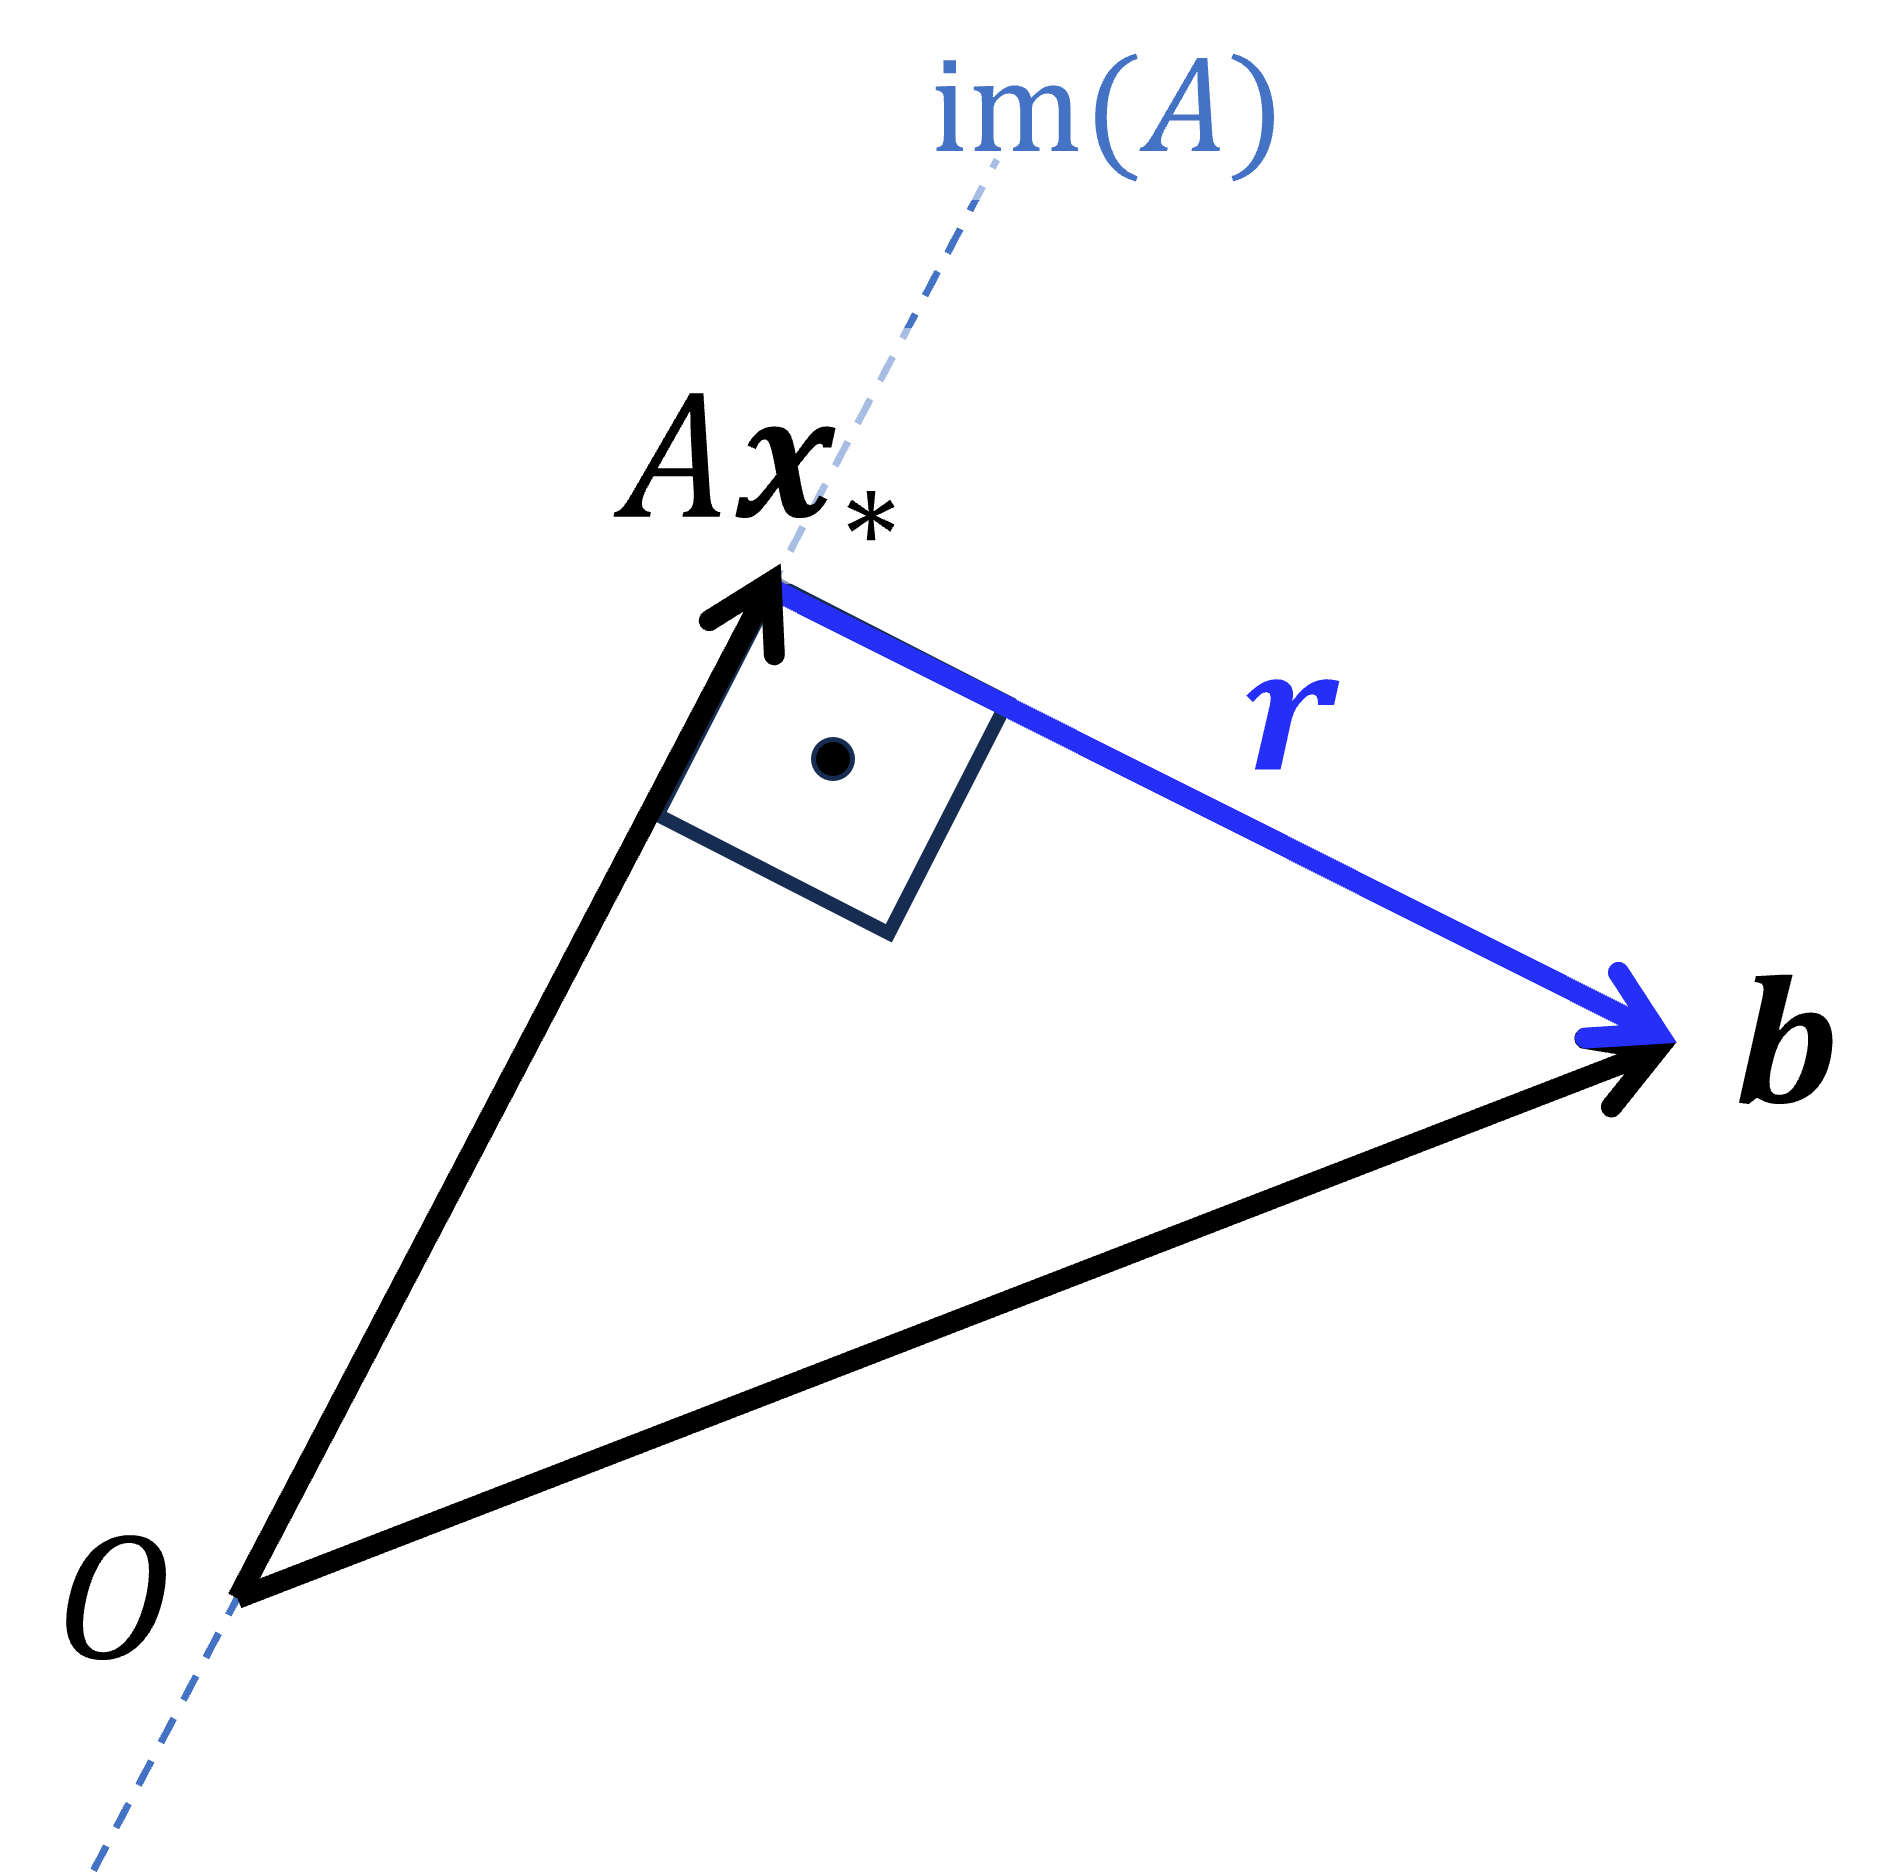
\includegraphics[width=\textwidth]{../Mathematik_2/Bilder/ausgleichsrechnung_residuum_orthogonal_zum_bildraum.png}
%\end{minipage}
%\begin{minipage}{0.65\textwidth}
%	Gegeben ist
%	\begin{itemize}
%		\item eine Matrix \(A\in\mathbb R^{n\times m}\) und
%		\item ein Vektor \(\boldsymbol b\in\mathbb R^n\) und
%		\item die L�sung \(\boldsymbol x_*\in\mathbb R^m\) der Normalengleichung.
%	\end{itemize}
%
%	Zeigen Sie, dass die folgenden Zusammenh�nge zwischen \(A\,\boldsymbol x_*\) und \(\boldsymbol r\) gelten:
%	\begin{itemize}
%		\item[(i)] Die L�nge des Residuums wird durch die L�sung der Normalengleichung minimiert:
%			\[ \| \boldsymbol r\| = \mathrm{min}  \; \Leftrightarrow \; A^\intercal \, A \, \boldsymbol x_* = A^\intercal \, \boldsymbol b \,.\]
%		\item[(ii)] Der Vektor \(A\,\boldsymbol x_*\) ist die Orthogonalprojektion von \(\boldsymbol b\) auf \(\mathrm{im}(A)\).
%	\end{itemize}
%\end{minipage}
%	\noindent \textbf{Hinweis:} Betrachten Sie die Funktion \(E: \boldsymbol x \mapsto \| A\,\boldsymbol x - \boldsymbol b\|^2\) und bestimmen Sie die station�ren Punkte.
%\end{exercisebox}
 \newpage  % �berbestimmte GL, Normalengleichung, Ausgleichsgerade

\chapter{Fourieranalyse}
\section*{Leitidee}
Die Fourieranalyse beruht auf der Beobachtung, dass sich viele Signale als �berlagerung harmonischer Schwingungen darstellen lassen.  Sinus- und Kosinusfunktionen bilden dabei eine geeignete Basis, auf der komplexe Signale zerlegt werden k�nnen.

Diese Zerlegung l�sst sich als Projektion einer Funktion auf ein Orthonormalsystem harmonischer Schwingungen verstehen.  Dadurch wird ein Signal nicht mehr nur als Funktion im Zeitbereich betrachtet, sondern als Kombination einfacher Schwingungen unterschiedlicher Frequenzen.

In der komplexen Exponentialdarstellung lassen sich diese Basisfunktionen besonders elegant behandeln, da Differentiation, Integration und Superposition zu einfachen algebraischen Operationen werden. Die Eulersche Identit�t
\[
	e^{i\, x}=\cos(x)+i\, \sin(x)
\]
verkn�pft dabei die trigonometrische mit der komplexen Darstellung und macht die zugrunde liegende Struktur sichtbar.

\bigskip
\etocsettocstyle{\section*{Inhalt dieses Kapitels}}{}
\localtableofcontents
\newpage

\setcounter{def}{0} \setcounter{satz}{0} \setcounter{exa}{0} \section{Fourier-Reihen}\label{MA2-fourierreihen}

\begin{table}[H]
  \centering
  \begin{tabularx}{\textwidth}{@{}>{\raggedright\arraybackslash}X r@{}}
    \toprule
    \multicolumn{2}{c}{\textbf{�bersicht �ber Lernziele und Voraussetzungen}} \\
    \midrule
    \textbf{Lernziele} & \\[.5\normalbaselineskip]
    \tabitem Fourier-Koeffizienten periodischer Funktionen berechnen &\\
    \tabitem eine periodische Funktion aus ihrer Fourier-Reihe rekonstruieren &\\
    \tabitem zwischen reeller und komplexer Darstellung von Fourier-Reihen wechseln &\\
    \tabitem das Konvergenzverhalten einer Fourier-Reihe qualitativ beurteilen & \\[.5\normalbaselineskip]
    \midrule
    \textbf{Voraussetzungen} &  \\[.5\normalbaselineskip]
    \tabitem mit harmonischen Schwingungen umgehen k�nnen & \abschnittsverweis{MA1-trigonometrische-funktionen} \\
    \tabitem mit der komplexen Exponentialfunktion sicher umgehen k�nnen & \abschnittsverweis{MA1-komplexe-zahlen-polarform-und-euler} \\
    \tabitem Integrale berechnen k�nnen & \abschnittsverweis{MA2-integrationsregeln} \\
    \tabitem mit Skalarprodukten in Funktionenr�umen umgehen k�nnen  & \abschnittsverweis{MA2-integrierbare-funktionen} \\
    \tabitem Orthonormalit�t von Funktionen �berpr�fen k�nnen & \abschnittsverweis{MA2-integrierbare-funktionen} \\[.5\normalbaselineskip]
    \bottomrule
  \end{tabularx}
\end{table}

\noindent \ifintegriereaufgaben Die �bungsaufgaben zum Thema finden Sie \hyperref[MA2-fourierreihen-aufgaben]{hier}.
\vspace{0.3cm}
\hrule
\fi

\subsection{Mathematisches Prisma}

Periodische Funktionen begegnen uns �berall in Natur und Technik: bei der Erdrotation, beim Herzschlag, bei elektrischen Wechselspannungen oder bei Licht- und Schallwellen. Trotz sehr unterschiedlicher physikalischer Hintergr�nde besitzen all diese Vorg�nge eine gemeinsame mathematische Struktur: Sie wiederholen sich nach einer festen Periode \(T\). Meist ist diese Periode eine Zeitdauer, sie kann jedoch ebenso gut ein Winkel oder eine r�umliche L�nge sein � etwa bei der Temperaturverteilung auf einem Metallring.

Die elementaren Bausteine solcher periodischen Vorg�nge sind \emph{harmonische Schwingungen}. Mathematisch haben sie die Form
\[
a\cdot \cos(\omega \cdot t)+b \cdot \sin(\omega \cdot t),
\]
also eine �berlagerung von Sinus- und Kosinusfunktionen mit Kreisfrequenz \(\omega\). Mithilfe der Eulerschen Formel lassen sich diese reellen Schwingungen\footnote{Die komplexe Darstellung macht deutlich, dass eine harmonische Schwingung einer rotierenden Bewegung in der komplexen Ebene entspricht.} �quivalent als komplexe Exponentialfunktionen schreiben:
\[
	a\cdot \cos(\omega \cdot t)+b \cdot \sin(\omega \cdot t) = c\cdot e^{i\omega \, t}+\overline c\cdot e^{-i\omega\, t}, \qquad c=\dfrac12\cdot (a-ib)\,.
\]

Viele physikalische Signale sind keine einzelnen harmonischen Schwingungen, sondern \emph{�berlagerungen} solcher Grundbausteine. Ein klassisches Beispiel ist wei�es Licht.

\begin{exabox}{Frequenzzerlegung durch ein Prisma}{}
\begin{minipage}{0.5\textwidth}
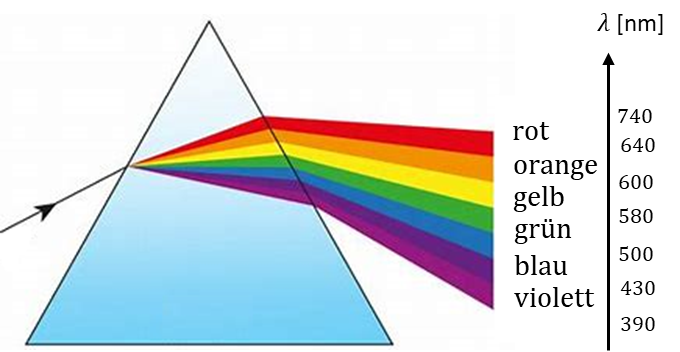
\includegraphics[width=\textwidth]{../Mathematik_2/Bilder/fourieranalyse_prisma_spektralzerlegung.png}
\end{minipage}
\begin{minipage}{0.5\textwidth}
Wei�es Licht wird im Prisma in seine Spektralfarben zerlegt. Unterschiedliche Wellenl�ngen werden unterschiedlich stark gebrochen. Physikalisch bedeutet das: Wei�es Licht ist eine �berlagerung harmonischer elektromagnetischer Wellen mit verschiedenen Frequenzen.

Genau diese Idee � ein Signal in seine Frequenzbestandteile zu zerlegen � verfolgt die Fourier-Analyse.
\end{minipage}
\end{exabox}
\bigskip

Die Fourier-Analyse beantwortet die Frage:
\begin{center}
\emph{Welche Sinus- und Kosinus-Anteile stecken in einem periodischen Signal \(u\)?}
\end{center}


\subsection{Fourierkoeffizienten}

Sei \(u(t)\) ein \(T\)-periodisches Signal. Dann lautet seine Fourier-Reihe formal
\begin{equation}\label{FR_formal}
u(t)
=
\dfrac{a_0}{2}
+
\sum_{n=1}^{\infty}
\left(
a_n \cdot \cos(n\cdot \omega_0 \, t)
+
b_n \cdot \sin(n\cdot \omega_0 \, t)
\right),
\qquad
\omega_0=\frac{2\pi}{T} \,.
\end{equation}

\begin{itemize}
\item \(\frac{a_0}{2}\) ist der Gleichanteil (Mittelwert �ber eine Periode).
\item Die Koeffizienten \(a_n\) und \(b_n\) sind die Amplituden der jeweiligen Kosinus- bzw. Sinusanteile.
\end{itemize}


Die Zahl \(\omega_0\) nennnt man die \emph{Grundkreisfrequenz} und die zugeh�rigen Funktionen
\[
\cos(\omega_0 \,t)
\quad \text{und} \quad
\sin(\omega_0 \, t)
\]
hei�en die \emph{Grundschwingung}. Die Grundschwingungen besitzen die kleinste Periode \(T\) und damit die kleinste im Signal vorkommende Frequenz.

Multipliziert man die Grundkreisfrequenz mit einer nat�rlichen Zahl \(n\), so erh�lt man
\[
	\omega_n = n \cdot \omega_0, \qquad n\in\mathbb N^+ \,.
\]
Die Funktionen
\[
\cos(\omega_n t)
\quad \text{und} \quad
\sin(n\omega_n t)
\]
hei�en Oberschwingung, die \emph{\(n\)-te harmonische Schwingung} oder kurz die \emph{\(n\)-te Harmonische}.

Alle Harmonischen sind ebenfalls \(T\)-periodisch, durchlaufen die Periode \(T\) jedoch \(n\)-mal schneller als die Grundschwingung. Mit wachsendem \(n\) steigt also die Frequenz, w�hrend die Periode gleich bleibt.

\begin{center}
	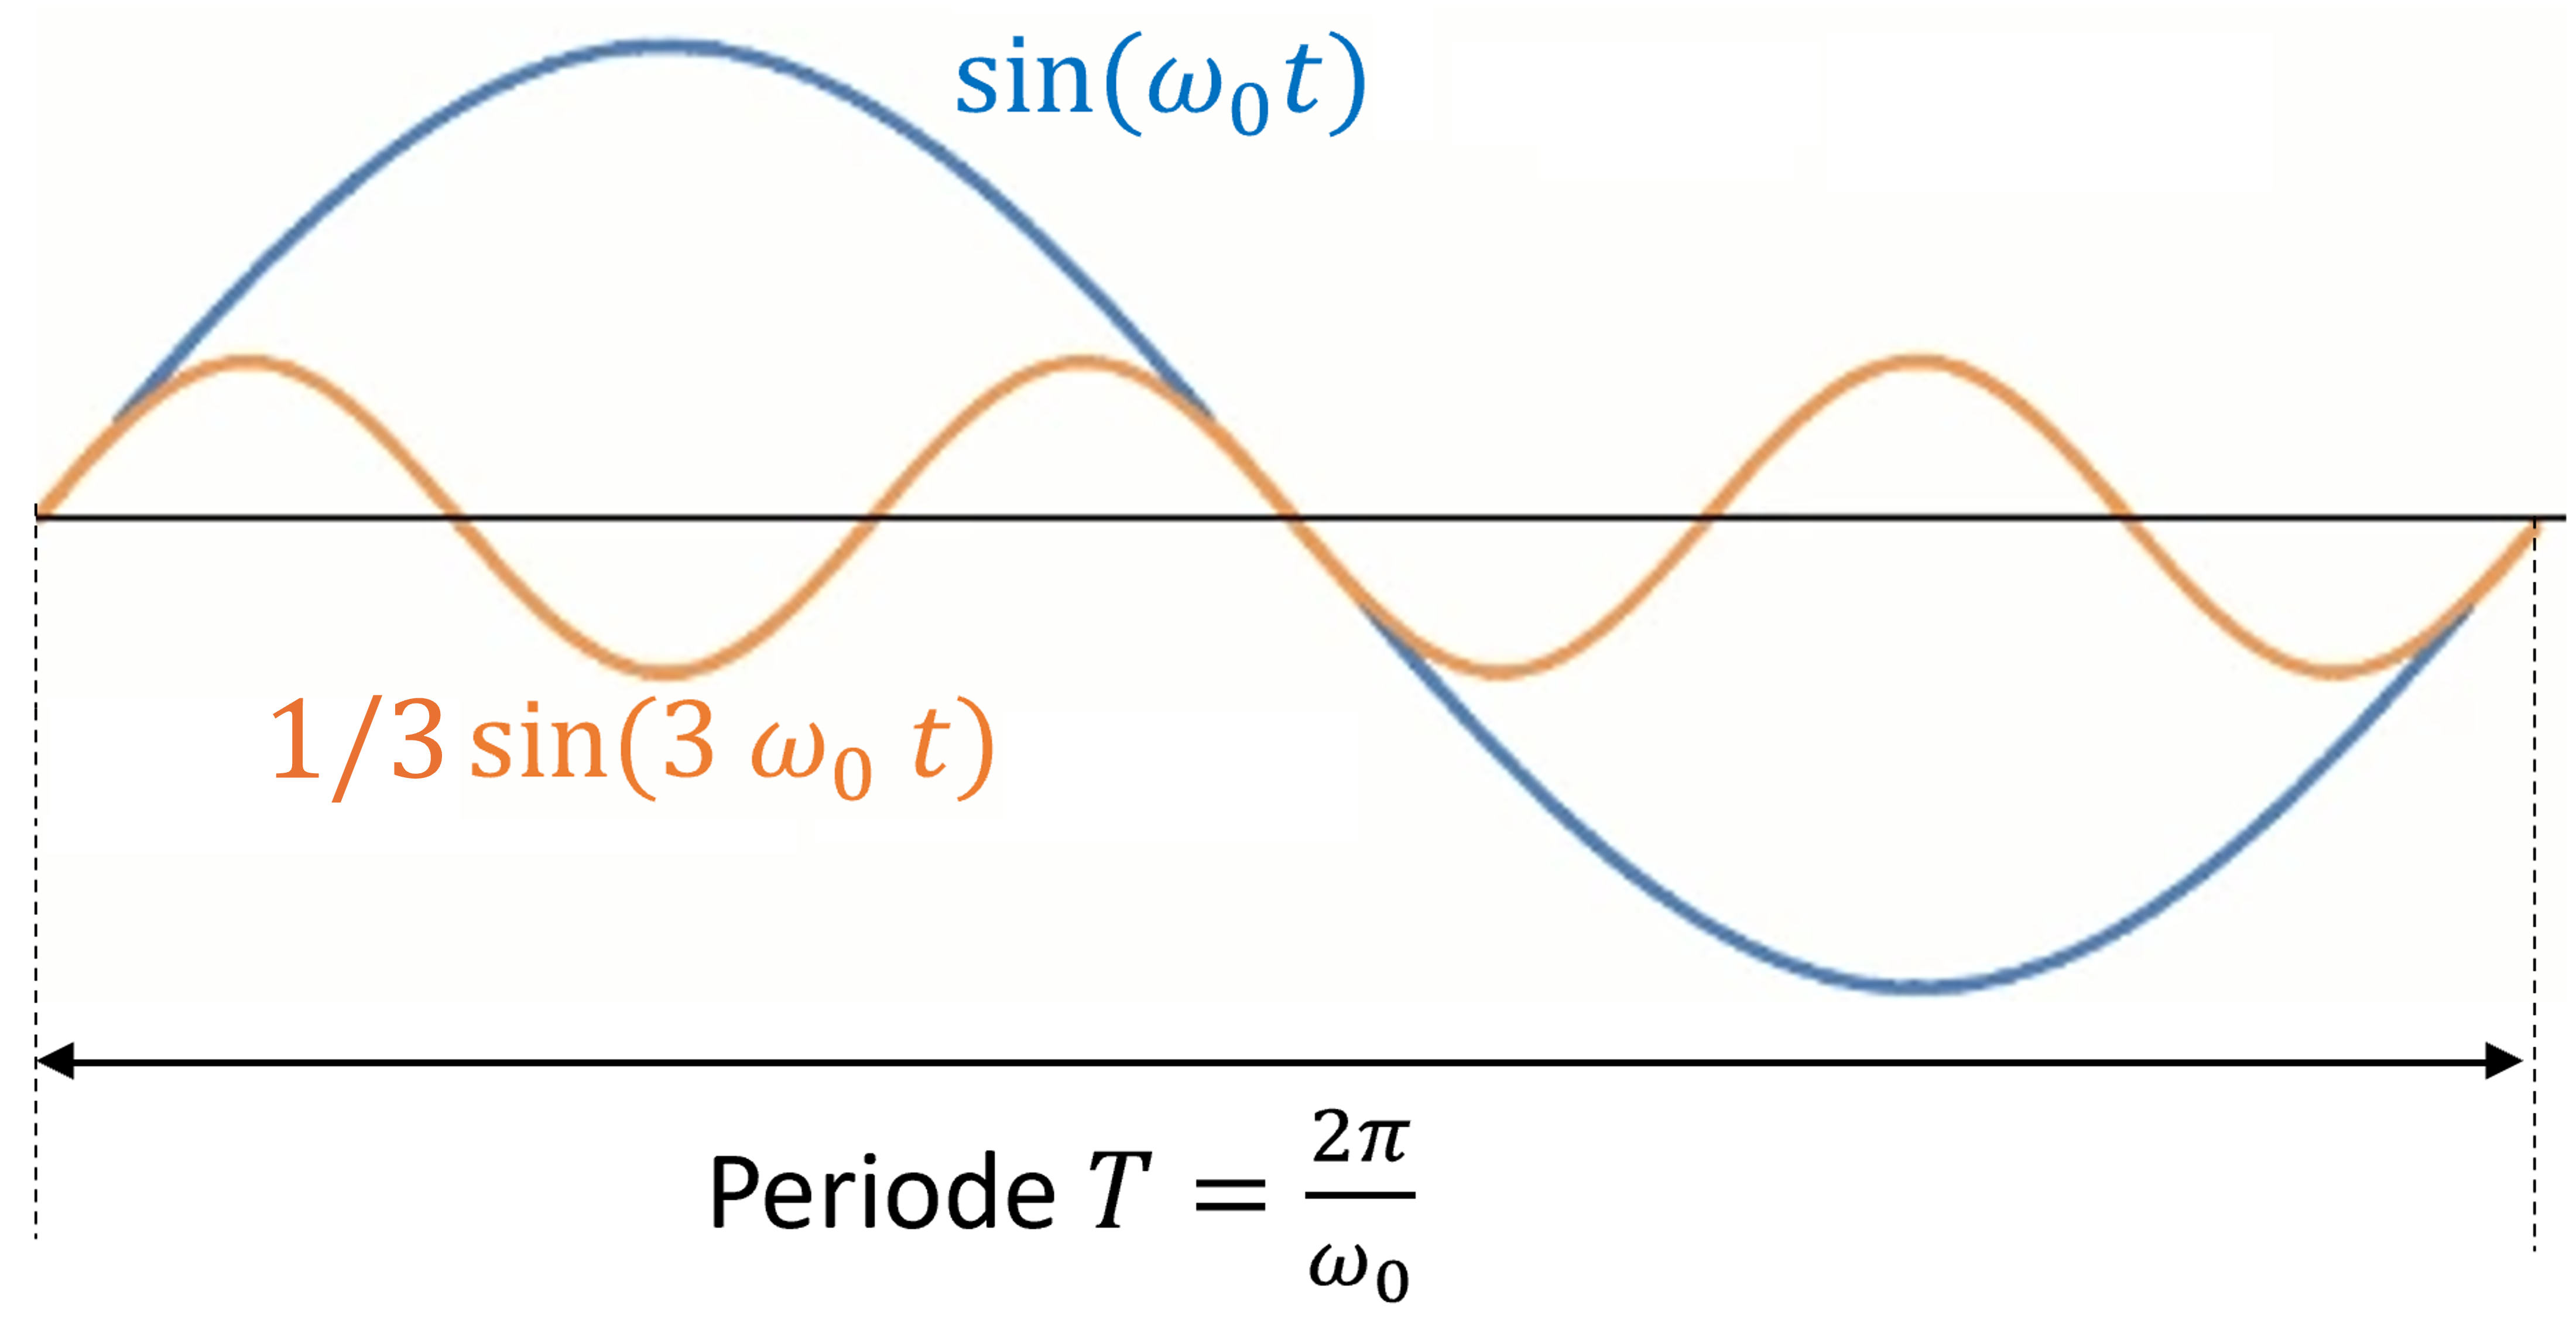
\includegraphics[width=0.7\textwidth]{../Mathematik_2/Bilder/harmonische_schwingungen_grund_und_oberschwingung.png}
\end{center}

Die Fourier-Reihe ist eine Superposition von unendlich vielen harmonischen Schwingungen - kennt man die Grundkreisfrequenz \(\omega_0\), dann ist die Struktur der Fourier-Reihe festgelegt. Einzig die Amplituden der harmonischen Schwingungen sind variabel! Die Gesamtheit der Amplituden, also der Zahlen \(a_n\) und \(b_n\) nennt man das \emph{Spektrum} des Signals. Kennt man das Spektrum, so kennt man das Signal � genau wie beim Prisma die Kenntnis der Spektralfarben die Zusammensetzung des wei�en Lichts beschreibt.

\bigskip

\begin{exabox}{Fourierpolynom eines Rechtecksignals mit Periode \(2\pi\)}{}
Wir betrachten die \(2\pi\)-periodische Fortsetzung
\[
u_T(t)=
\begin{cases}
1,& t\in[0,\pi),\\
-1,& t\in[\pi,2\pi).
\end{cases}
\qquad
(T=2\pi,\;\omega_0=1).
\]

\begin{center}
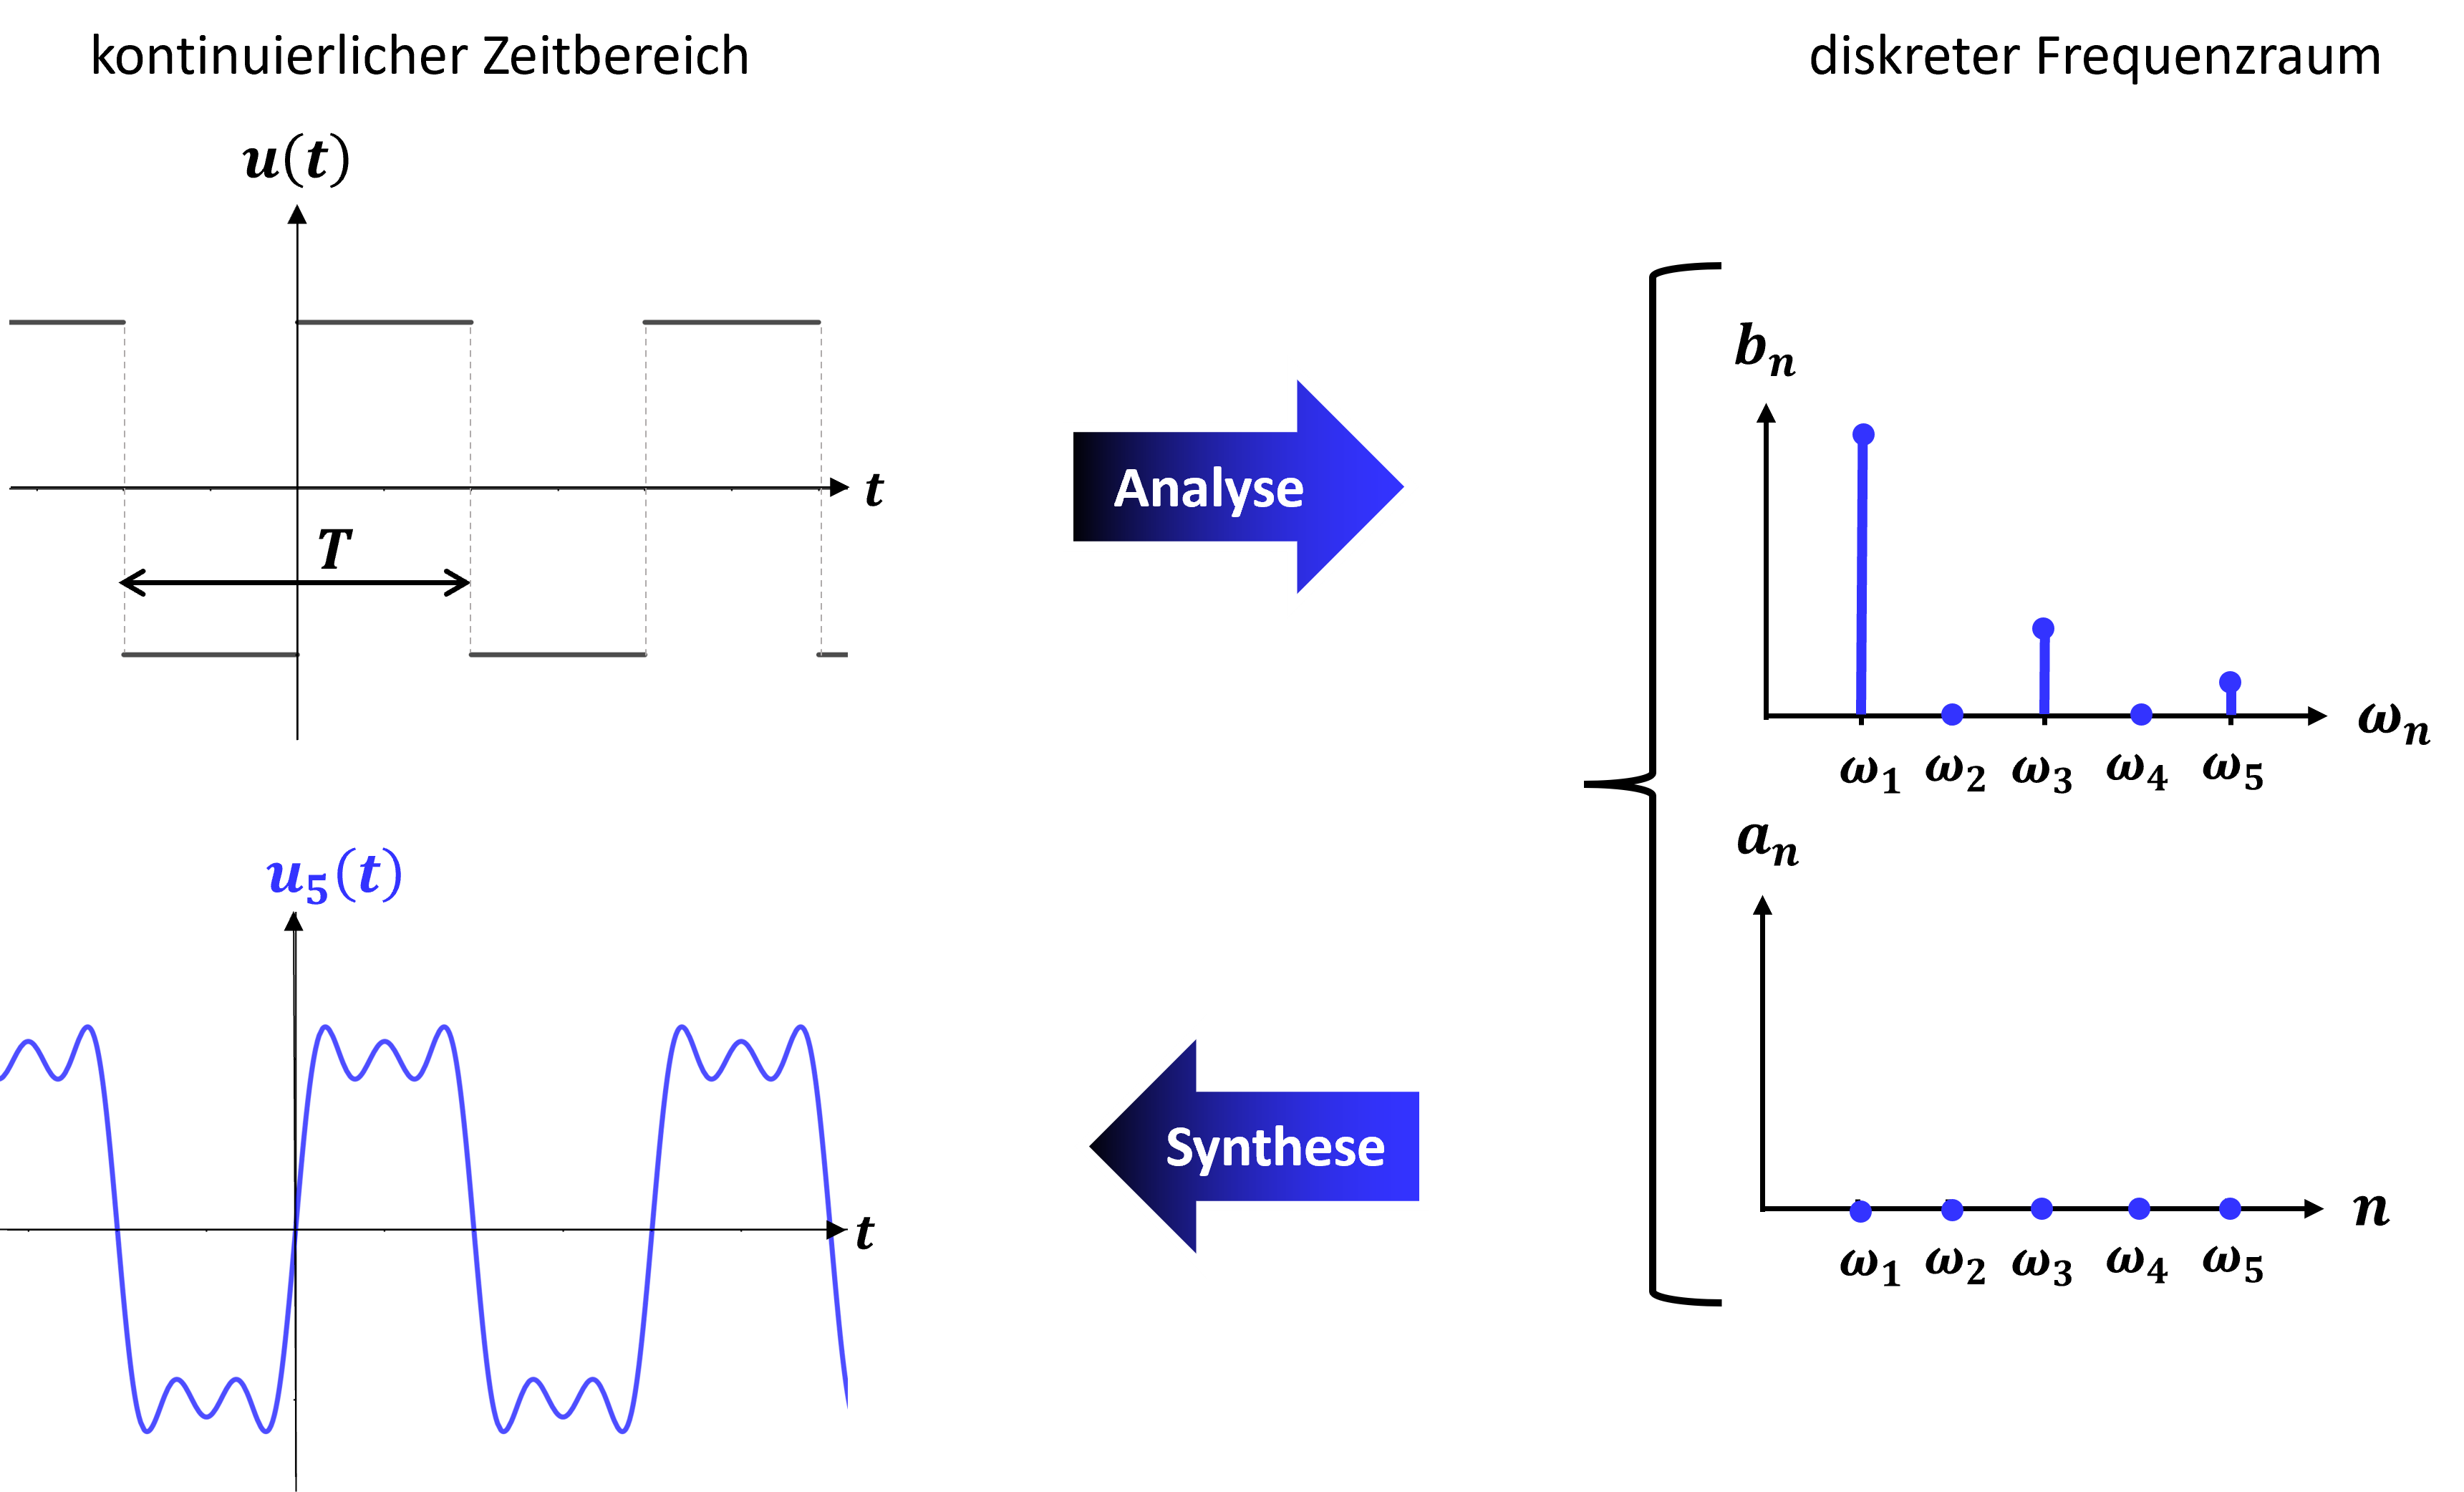
\includegraphics[width=0.8\textwidth]{../Mathematik_2/Bilder/fourierreihe_analyse_und_synthese.png}
\end{center}

Dieses Signal besitzt folgende Eigenschaften:

\begin{itemize}
	\item Der Mittelwert ist null, also \(\textcolor{blue}{a_0}=\textcolor{blue}{0}\).
\item Wegen der Punktsymmetrie treten keine Kosinusanteile auf: \(\textcolor{blue}{a_n} = \textcolor{blue}{0}\).
\item Es erscheinen nur ungerade Sinusanteile.
\end{itemize}

Die Fourier-Synthese bis zur f�nften Harmonischen lautet
\[ \begin{array}{rcl l }
u_5(t) &=&  \dfrac{\textcolor{blue}{a_0} }{2} +  \displaystyle\sum\limits_{n=1}^5 \textcolor{blue}{a_n} \, \cos( n\, t) + \textcolor{blue}{b_n} \, \sin( n\, t) &\|\; \textcolor{blue}{a_n} = \textcolor{blue}{0}, n=0,1,2,3,4,5 \\[2ex]
&=&  \displaystyle\sum\limits_{n=1}^5 \textcolor{blue}{b_n} \, \sin( n\, t) &\|\;  \textcolor{blue}{b_n} = \textcolor{blue}{0}, n=2,4 \\[2ex]
&=& \textcolor{blue}{b_1} \,\sin(t) + \textcolor{blue}{b_3} \,\sin(3\,t) + \textcolor{blue}{b_5} \,\sin(5\,t)  &\\[2ex]
&=& \textcolor{blue}{1.27324} \,\sin(t) + \textcolor{blue}{0.42441}\,\sin(3\,t) + \textcolor{blue}{0.25465}\,\sin(5\,t)\,. &
\end{array}\]

Mit wachsender Frequenz nehmen die Amplitude ab. Die Summe weniger Harmonischer liefert bereits eine gute Approximation des Signals.
\end{exabox}


Die harmonischen Schwingungen mit Periode \(T\) bilden bez�glich des Skalarprodukts
\begin{equation}\label{skalarprodukt_fr_reell} \langle u, v \rangle = \dfrac{2}{T} \cdot \int\limits_0^{T}  u(t) \cdot v(t) \,\mathrm d t\,,\end{equation}
ein \underline{Orthonormalsystem}\randverweis{MA2-integrierbare-funktionen}. Genau hier liegt der strukturelle Kern der Fourier-Theorie.

\bigskip
\noindent \textbf{Projektionsprinzip aus der linearen Algebra}
\bigskip

Ist \(\{\hat e_1,\dots, \hat e_n\}\) eine Orthonormalbasis eines endlichdimensionalen Vektorraums und
\[
	\vec v=\sum_{k=1}^n v_k \cdot \hat e_k\,,
\]
so gilt
\[
	v_k=\langle \vec v,\hat e_k\rangle \,.
\]
Die Koeffizienten entstehen also durch Orthogonalprojektion auf die Basisvektoren und genau dasselbe passiert im Funktionenraum.

\bigskip
\noindent \textbf{Projektionsprinzip f�r Fourier-Polynome}
\bigskip

Betrachten wir ein Fourier-Polynom vom Grad \(N\)
\[\begin{array}{rcl l}
p(t) &=&  \dfrac{a_0}{2} + \displaystyle\sum\limits_{n=1}^{N} \bigl( a_n \cdot \cos(\omega_n \, t)  + b_n \cdot  \sin(\omega_n \, t) \bigr) & \|\; \textnormal{Fokus harmonische Schwingungen} \\[2ex]  &=&  \dfrac{a_0}{2} + \displaystyle\sum\limits_{n=1}^{N} \bigl( a_n \cdot \hat c_n  + b_n \cdot \hat s_n \bigr) & \|  \; \textnormal{Fokus orthonormierte Vektoren}\,. \end{array} \]

Wenn das Projektionsprinzip gilt, dann m�ssten wir zeigen k�nnen, dass folgendes gilt:
\[
	a_3=\langle p,\hat c_3\rangle\,.
\]

Wir kennen das Skalarprodukt und wir wissen wie \(p\) aussieht - dann haben wir alles beisammen, um diese Behauptung zu pr�fen.

\bigskip
\noindent \textbf{1. Einsetzen des Polynoms und Ausnutzen der Linearit�t des Skalarprodukts}
\bigskip

Das Skalarprodukt ist linear im ersten Argument. Daher d�rfen wir die Summe auseinanderziehen:

\[ \begin{array}{rcl}
		\langle p,\hat c_3\rangle &= & \left\langle \dfrac{a_0}{2} + \displaystyle\sum_{n=1}^{N} \bigl( a_n \cdot \hat c_n + b_n \cdot \hat s_n \bigr), \hat c_3 \right\rangle \\[2ex]
		&=& \textcolor{blue}{\dfrac{a_0}{2}\,\langle 1 , \hat c_3\rangle + \displaystyle\sum_{n=1}^{N} a_n \cdot \langle \hat c_n, \hat c_3\rangle + \displaystyle\sum_{n=1}^{N} b_n \cdot  \langle \hat s_n, \hat c_3\rangle }
\end{array} \]


\bigskip
\noindent \textbf{2. Eigenschaften des Orthonormalsystems ausnutzen}
\bigskip

Die Funktionen
\[ 1, \hat c_n(t), \hat s_n(t), n\in\mathbb N^+\,, \quad  \begin{cases} \hat c_n(t) & = \cos(n \omega_0 \, t) \,, \\[1ex] \hat s_n(t) &= \sin(n \omega_0\, t)\,, \end{cases}\]
sind bez�glich des Skalarprodukts \ref{skalarprodukt_fr_reell} paarweise orthonormal und aus diesem Grund gilt:

\[
	\begin{array}{rcl}
		\langle 1 ,\hat c_3\rangle &=& \dfrac{2}{T} \cdot \displaystyle \int\limits_{0}^T 1 \cdot \cos(\omega_3 \, t)\, \mathrm d t =  0\,, \\[2ex]
		\langle \hat s_n ,\hat c_3\rangle &=& \dfrac{2}{T} \cdot \displaystyle \int\limits_{0}^T \sin(\omega_n \, t) \cdot \cos(\omega_3 \,t)\, \mathrm d t =  0\,, \quad n \geq 1 \\[2ex]
		\langle \hat c_n ,\hat c_3\rangle &=& \dfrac{2}{T} \cdot \displaystyle \int\limits_{0}^T \cos(\omega_n \, t) \cdot \cos(\omega_3 \,t)\, \mathrm d t  = \begin{cases} 1, & n=3,\\ 0, & n\neq 3\,.  \end{cases}
	\end{array}
\]

Damit bleibt in der obigen \textcolor{blue}{Summe} genau ein einziger Summand �brig, n�mlich der f�r \(n=3\) und es gilt

\[
	\textcolor{blue}{\langle p,\hat c_3\rangle} = \dfrac{a_0}{2}\,\langle 1,\hat c_3\rangle + \sum_{n=1}^{N} a_n \cdot \langle \hat c_n, \hat c_3\rangle + \sum_{n=1}^{N} b_n \cdot \langle \hat s_n,\hat c_3\rangle = a_3\cdot  \langle \hat c_3, \hat c_3\rangle = a_3\,.
\]

Gleichzeitig haben wir eine konkrete Berechnungsformel f�r den Fourierkoeffizient \(a_3\)! Setzen wir das Skalarprodukts in dem \textcolor{blue}{Ausdruck} links erhalten wir

\[
a_3 =\textcolor{blue}{\langle p, \hat c_3\rangle} = \frac{2}{T} \cdot \int\limits_0^T p(t)\cdot \cos(\omega_3 \,t)\,\mathrm d t\,.  \]

\bigskip
\noindent \textbf{Interpretation}
\bigskip

\begin{itemize}
	\item Der Koeffizient \(a_3\) misst den Anteil der Schwingung \(\hat c_3\) im Signal \(p\).
	\item Das Integral ist nichts anderes als die Orthogonalprojektion von \(p\) auf diese Basisfunktion.
\end{itemize}

Was wir f�r den Koeffizienten \(a_3\) explizit durchdacht haben, gilt f�r alle anderen Koeffizienten eines Fourierpolynoms:
\[
	\begin{array}{rcl}
p(t)
&=&
\dfrac{a_0}{2}
+
\displaystyle \sum\limits_{n=1}^{N}
\left(
	a_n\cdot \cos(\omega_n \, t)
+
b_n \cdot \sin(\omega_n\, t)
\right) \\
&=&
\dfrac{a_0}{2}
+
\displaystyle\sum\limits_{n=1}^{N}
\left(
	a_n\cdot \hat c_n + b_n \cdot \hat s_n
\right) \quad \textnormal{mit } \quad  \begin{cases} a_0 = \langle p, 1\rangle\,, \\ a_n = \langle p,\hat c_n\rangle\,, \\  b_n=\langle p,\hat s_n\rangle\,.\end{cases}
\end{array}\]

F�r eine beliebige \(T\)-periodische, st�ckweise stetig differenzierbare Funktion \(u\), definieren wir die  Fourier-Koeffizienten ganz genauso:
\[
a_n
=
\frac{2}{T}
\int\limits_0^T
u(t)\cdot \cos(\omega_n \, t)\,\mathrm dt,
\qquad
b_n
=
\dfrac{2}{T}
\int\limits_0^T
u(t)\cdot \sin(\omega_n \, t)\,\mathrm dt\,,
\]

und auch deren Interpretation �bertr�gt sich auf den allgemeinen Fall:

\begin{itemize}
	\item Die Fourierkoeffizienten sind Projektionen von \(u\) auf die jeweilige Basisfunktion.
	\item Unter Fourier-Analyse verstehen wir die Bestimmung der Fourierkoeffizienten \(b_n, n\geq 0\) und \(a_n, n\geq 1\).
	\item Die Menge aller Fourierkoeffizienten nennt man das Spektrum des Signals.
	\item Das Spektrum ist diskret und umfasst im Allgemeinen unendlich viele Zahlen. Man sagt es ist unendlich.
	\item Kennt man das Spektrum, so kennt man die Zerlegung des Signals in harmonische Schwingungen.
	\item Ist \(u-\dfrac{a_0}{2}\) \underline{gerade}, so verschwinden alle \(b_n\). \randverweis{MA1-eigenschaften-von-funktionen}
	\item Ist \(u-\dfrac{a_0}{2}\) \underline{ungerade}, so verschwinden alle \(a_n\). \randverweis{MA1-eigenschaften-von-funktionen}
\end{itemize}

\begin{exabox}{Spektrum eines Rechtecksignals mit Periode \(T=2\)}{}
Wir betrachten die \(2\)-periodische Fortsetzung
\[
u_T(t)=
\begin{cases}
1,& t\in[0,1),\\
0,& t\in[1,2).
\end{cases}
\qquad
(\omega_0=\pi).
\]

\textbf{Gleichanteil}
\[
a_0=\int\limits_0^1 1\,dt=1.
\]

\textbf{Kosinusanteile}
\[
a_n
=
\int\limits_0^1 \cos(n\pi t)\,dt
=
\Bigl[\frac{\sin(n\pi t)}{n\pi}\Bigr]_0^1
=
0\,, \; n\geq 1\,.
\]

\textbf{Sinusanteile}
\[
b_n
=
\int\limits_0^1 \sin(n\pi t)\,dt
=
\Bigl[\frac{-\cos(n\pi t)}{n\pi}\Bigr]_0^1
=
\frac{1-(-1)^n}{n\pi} = \begin{cases} 0, \quad n \textnormal{ gerade} \\ \frac{2}{n\pi},\quad n \textnormal{ ungerade}\,. \end{cases}
\]

Das Spektrum von \(u\) lautet \[ \left\{ b_{2n-1} =  \frac{2}{(2\,n-1)\,\pi}, \; n\in\mathbb N_0\right\}\,. \]
\end{exabox}
\bigskip


\subsection{Fourier-Reihe}

Formal l�sst sich aus einem gegebenen Spektrum, das zu einem Signal \(u\) geh�rt, die Fourier-Reihe zu \(u\) hinschreiben. Sie lautet:
\[
\mathrm{FR}_u(t)
=
\dfrac{a_0}{2}
+
\sum\limits_{n=1}^{\infty}
\left(
	a_n\cdot \cos(\omega_n\, t)
+
b_n\cdot \sin(\omega_n\, t)
\right).
\]
\bigskip

\begin{exabox}{Fourier-Reihe eines Signals}{}
\textbf{Gleichanteil}
\[ a_0 = 1 \]
\textbf{Spektrum}
\[ \left\{ b_{2n-1} =  \frac{2}{(2\,n-1)\,\pi}, \; n\in\mathbb N_0\right\}\,. \]
\textbf{Fourier-Reihe}
\[
\mathrm{FR}_u(t)
=
\dfrac12
+
\dfrac{2}{\pi}\sin(\pi \,t)
+
\dfrac{2}{3\pi}\sin(3\pi\, t)
+
\dfrac{2}{5\pi}\sin(5\pi \,t)
+\cdots\,.
\]
\end{exabox}
\bigskip

Die Tatsache, dass die Fourier-Reihe \(\mathrm{FR}_n\) und das Signal \(u\) miteinander verkn�pft sind, liegt auf der Hand, aber was hei�t das konkret?
\begin{center}
	\emph{Was hat die Fourier-Reihe eines Singals \(u\) mit der dem Signal \(u\) zu tun?}
\end{center}

Die Antwort ist: die Fourier-Reihe stellt das Signal fast �berall dar:

\begin{theorembox}{Konvergenz (Merksatzform)}{}
Sei $u$ $T$-periodisch und st�ckweise stetig differenzierbar. Dann gilt:
\begin{itemize}
\item Ist $u$ in $t_*$ stetig, so konvergiert die Fourier-Reihe $\mathrm{FR}_u(t_*)$ gegen $u(t_*)$.
\item An allen Sprungstellen konvergiert die Fourier-Reihe gegen den Mittelwert von links- und rechsseitigem Grenzwert von $u$.  Hat \(u\) in $t_*$ einen Sprung, so gilt also
\[
	\mathrm{FR}_u(t_*)=\frac12\cdot \left(\lim\limits_{t\uparrow t_*} u(t)+\lim\limits_{t\downarrow t_*} u(t)\right).
\]
\end{itemize}
\begin{figure}[H]
  \caption{Konvergenz der Fourier-Reihe an Sprungstellen}
  \centering
  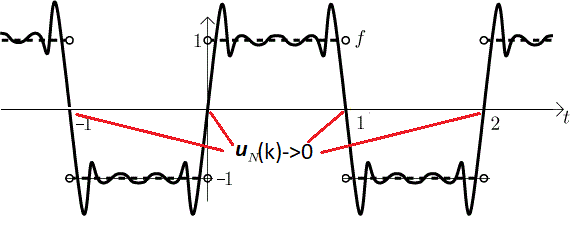
\includegraphics[width=0.5\textwidth]{../Mathematik_2/Bilder/fourierreihe_sprungstellen_positivitaet.png}
\end{figure}
\end{theorembox}

\bigskip
\noindent{\textbf{Bemerkungen:}}
\begin{itemize}
	\item Unter Fourier-Synthese verstehen wir die Rekonstruktion eines periodischen Signals bei gegebenem Spektrum.
	\item Das Ergebnis der Fourier-Synthese ist im Allgemeinen eine Fourier-Reihe, bricht man die Fourier-Reihe nach dem \(N\)-ten Glied ab, dann erh�lt man ein Fourier-Polynom.
	\item Die Fourier-Reihe ist eine Darstellungsform eines periodischen Singals, aus dem die Frequenzanteile, die im Signal vorhanden sind, ablesbar sind .
\end{itemize}


\subsection*{Komplexe Fourier-Reihe}
\paragraph{Exponentialdarstellung von Schwingungen}

Sinus und Kosinus k�nnen als Real- und Imagin�rteil einer komplexen Exponentialfunktion geschrieben werden\wennreferenzvorhanden{MA1-komplexe-zahlen-polarform-und-euler}{ (vgl. Abschnitt \abschnittsverweis{MA1-komplexe-zahlen-polarform-und-euler})}:

\[
e^{i\omega t}=\cos(\omega t)+i\sin(\omega t).
\]

Damit lassen sich harmonische Schwingungen auch als komplexe Exponentialfunktionen darstellen.

Der gro�e Vorteil dieser Darstellung ist:
Exponentialfunktionen lassen sich besonders einfach differenzieren und miteinander kombinieren.

Aus diesem Grund formuliert man viele Ergebnisse der Fourier-Analyse
und der Systemtheorie in der Form

\[
e^{i\omega t}.
\]

Die trigonometrischen Funktionen erscheinen dann automatisch als Real- oder Imagin�rteil.

Da die Funktionen
\[
	\hat \varphi_k: \mathbb R \to \mathbb C, t\mapsto e^{ik\omega_0\, t},\qquad k\in\mathbb Z\,,
\]
bez�glich des Skalarprodukts
\[
\langle u,v\rangle:=\frac{1}{T}\int\limits_0^T u(t)\,\overline{v(t)}\,\mathrm dt.
\]
orthonormiert sind, l�sst sich das Konstruktionsprinzip einfach �bertragen: F�r ein \(T\)-periodisches Signal definieren wir die Fourier-Koeffizienten als Projektion von \(u\) auf die Basisfunktion \(\hat \varphi_k\)
\[
	c_k=\langle u,\hat \varphi_k\rangle=\frac{1}{T}\int\limits_0^T u(t)\,e^{-ik\omega_0 t}\,\mathrm dt\,,
\]
und die Fourier-Reihe lautet entsprechend
\[
	\mathrm{FR}_u(t)=\sum_{k=-\infty}^{\infty} c_k\,e^{ik\omega_0 \,t}\,..
\]
Die komplexe Form der Fourier-Reihe ist �quivalent zur reellen Darstellung und wird h�ufig f�r Rechnungen und in der Signalverarbeitung verwendet.

\begin{exabox}{Fourier-Reihe eines Rechtecksignals mit Periode \(T=2\)}{ }
	\(2\)-periodische Fortsetzung der Funktion:
	\begin{eqnarray*}
		u: [0,2)\to \mathbb R, t\mapsto  \begin{cases} 1,\quad &t\in ([0, 1)\,,\\
			0,\quad &t\in [1,2)\end{cases} \,.
			\end{eqnarray*}
			Grundfrequenz : \(\omega_0 = \dfrac{2\pi}{2} = \pi\,.\)

			\noindent Komplexe Fourier-Koeffizienten:
			\begin{eqnarray*}
				c_0 &=& \frac12\int\limits_{0}^2 u(t)\, \mathrm{d}t = \frac12\int\limits_{0}^1 \, \mathrm{d}t = \frac12\,,\\
				c_k &=& \frac12\int\limits_{0}^2 u(t) \cdot e^{-i\, k\, \pi t} \, \mathrm{d}t = \frac12 \, \int\limits_{0}^1 e^{-i\,k\,\pi\, t} \, \mathrm{d}t = \frac12\, \left[ \frac{e^{-i\, k \,\pi \, t}}{-i \, k \, \pi}\right]_0^1 = \frac12\, \frac{1-(-1)^k}{ i \,k\, \pi} = \begin{cases} \displaystyle{\frac{1}{ i\, k\pi}}, \quad & k\; \textnormal{ungerade} \,,\\
				0, \quad & k\; \textnormal{gerade}\,.\end{cases} \\ &&\Rightarrow c_{2k+1} = \frac{1}{i \,(2\,k+1) \,\pi}\,.
			\end{eqnarray*}
			L�sung:
			\begin{eqnarray*}
				\mathrm{FR}_u(t) &=& \frac12 +\sum\limits_{k \in \mathbb Z\setminus\{0\} } \frac{1}{i \, (2 \, k+1) \, \pi} \cdot e^{i \,  (2\, k+1) \, \pi \, t} \\
				&=& \frac12 + \sum\limits_{k = 1}^{\infty} \left( \frac{1}{i\, (2\, k+1) \, \pi} \cdot e^{i \, (2\,k +1) \, \pi \, t} - \frac{1}{i \, (2\,k+1)\, \pi} \cdot e^{-i\pi (2k +1)t} \right) \\
				&=& \frac12 + \sum\limits_{k = 1}^{\infty}\frac{1}{i (2k+1) \pi} \cdot   \underbrace{\left( e^{i \,\pi \, (2 \,k +1) \,t} -  e^{-i \, (2k +1) \,\pi \,t}\right)}_{\displaystyle{ = 2\,i \cdot \sin\left( (2k+1) \, \pi t\right)} } \\
				&=& \frac12 + \frac2\pi\sum\limits_{k = 1}^{\infty}\frac{1}{2\, k+1} \cdot  \sin\left( (2\, k+1) \,\pi\, t\right)\,.
			\end{eqnarray*}

		\end{exabox}

\subsection{Zusammenfassung}

In der linearen Algebra haben wir gelernt, dass ein Vektorraum besonders �bersichtlich wird, wenn wir eine \emph{Orthonormalbasis} kennen. Ist $\{\hat e_1,\dots, \hat e_n\}$ eine Orthonormalbasis des $\mathbb R^n$, so besitzt jeden Vektor $\vec v \in \mathbb R^n$ in dieser Basis eine eindeutige Darstellung und die lautet

\[
	\vec v = \sum\limits_{k=1}^n \underbrace{ \langle v,\hat e_k\rangle}_{\displaystyle{=v_k}} \, \hat e_k\,.
\]

Die Koeffizienten \(v_k, \, k=1,\cdots,n\) entstehen durch Projektion mithilfe des Skalarprodukts und die Orthogonalit�t der Basisvektoren sorgt daf�r, dass sich die einzelnen Komponenten nicht gegenseitig beeinflussen.

Dasselbe Strukturprinzip haben wir auf periodische Funktionen �bertragen, wobei folgende Analogien gelten

\begin{center}
\begin{tabular}{l c l}
$\mathbb R^n$ & & Funktionenraum \\[6pt]
\hline
Vektor $\vec v$ & $\longleftrightarrow$ & Periodische Funktion $u$ \\[6pt]
Einheitsvektoren $\{\vec e_k\,, k=1,\cdots,n\}$ & $\longleftrightarrow$ & Basisfunktionen $\{\hat \varphi_k \; k\in \mathbb Z\}$ \\[6pt]
Skalarprodukt Summe & $\longleftrightarrow$ & Skalarprodukt Integral \\[6pt]
Zerlegungskoeffizient $v_k = \langle \vec v,\vec e_k\rangle$ & $\longleftrightarrow$ & Fourier-Koeffizient \(c_k = \langle u, \hat \varphi_k\rangle\)\\[6pt]
Zerlegung $ \vec v = \sum\limits_{k=1}^n v_k \cdot \hat e_k $ & $\longleftrightarrow$ & Zerlegung \( u \approx \mathrm{FR}_u = \sum\limits_{k=-\infty}^\infty c_k \cdot \hat \varphi_k \)
\end{tabular}
\end{center}

\bigskip
\noindent \textbf{Bemerkungen:}

\begin{itemize}
	\item Harmonische Schwingungen spielen im Funktionenraum dieselbe Rolle wie Einheitsvektoren im $\mathbb R^n$.
	\item Wie im endlichdimensionalen Fall entstehen die �Koordinaten� einer Funktion durch Projektion.
	\item F�r eine geeignete periodische Funktion l�sst sich formal eine Fourier-Reihe entwickeln.
	\item Die Fourier-Reihe ist eine �berlagerung von im Allgemeinen unendlich vielen harmonischen Schwingungen mit gleicher Periode.
	\item Die Fourier-Reihe stellt die Ausgangsfunktion fast �berall dar.
\end{itemize}

\bigskip
\noindent \textbf{Formeln kompakt:}

\begin{theorembox}{Fourier-Reihe}{}
\begin{itemize}
\item $\omega_0=\dfrac{2\pi}{T}$
\item $\omega_k=k\cdot \dfrac{2\pi}{T}, \quad k\in \mathbb Z$
\item Reelle Fourier-Reihe:
\[
	\mathrm{FR}_u(t)=\frac{a_0}{2}+\sum_{n=1}^{\infty}\bigl(a_n\cdot \cos(n\omega_0 t)+b_n \cdot \sin(n\omega_0 t)\bigr)\,,\; \textnormal{mit}
\]
\[
	a_0=\frac{2}{T}\int_0^T u(t) \, \mathrm d t,\quad
	a_n=\frac{2}{T}\int_0^T u(t) \cdot \cos(\omega_n\, t) \, \mathrm d t ,\quad
	b_n=\frac{2}{T}\int_0^T u(t) \cdot \sin(\omega_n\, t)\, \mathrm d t
\]
\item Komplexe Fourier-Reihe:
\[
	\mathrm{FR}_u(t)=\sum_{k=-\infty}^{\infty}c_k \cdot e^{i\,\omega_k\, t},
\qquad
c_k=\frac{1}{T}\int_0^T u(t) \cdot e^{- i\omega_k\, t}\,\mathrm d t.
\]
\end{itemize}
\end{theorembox}

 \newpage % 10 Fourierreihen
%\setcounter{exercise}{0} 
%\subsection{Vokabular}
%\beign{itemize}
%\item Spektrum
%\item Fourier-Theorie vs Potenzreihen
%\item Analyse und Synthese
%\item Schwingende Saite
%\item Partielle Differentialgleichung
%\item Diskrete Energiezust�nde
%\item Randbedingung
%\item Separationsl�sung
%\item Darstellung von Grundschwingung und Oberschwingungen: Beobachtung (Randbedingungen!)
%\item Wavelets
%\item Vektorraum, additive geschlossen
%\item Periode
%\item Bestapproximation mit trigonometrischen Funktionen
%\item Konvergenzverhalten der Fourier-Reihe
%\item Vollst�ndigkeit?
%	\end{itemize}

\ifintegriereaufgaben

\section*{Fourierreihen Aufgaben}\label{MA2-fourierreihen-aufgaben}
Erkl�rungen und Beispiele, die zur Bearbeitung der Aufgaben hilfreich sind, finden Sie im Skript\wennreferenzvorhanden{MA2-fourierreihen}{ (Abschnitt \abschnittsverweis{MA2-fourierreihen})} und, falls Sie nicht weiterkommen, dann schauen Sie \hyperref[MA2-fourierreihen-loesungen]{hier}.
\else
\section{Fourierreihen Aufgaben}\label{MA2-fourierreihen-aufgaben}

Regeln und Beispiele zu diesen Aufgaben finden Sie im Skript. Die L�sungen finden Sie \hyperref[MA2-fourierreihen-loesungen]{hier}.
\fi

	\begin{exercisebox}[Harmonische Schwingungen]
		Bestimmen Sie die Amplitude, die Periode und die Nullphase der folgenden harmonischen Schwingungen und skizzieren sie den Funktionsverlauf
		\begin{eqnarray*}
		(a)\; y(t) = 2\,\sin\left(3\, t-\dfrac{\pi}{6} \right)\quad \quad (b)\; y(t) = 10\,\sin\left(\pi\, t - 3\,\pi\right)\,.
		\end{eqnarray*}
\end{exercisebox}

	\begin{exercisebox}[komplexes Fourier-Polynom vs. reelles Fourier-Polynom]
		\begin{itemize}
			\item[(a)]
		Zeigen Sie, dass man die komplexwertigen Koffizienten $c_k$ eines komplexen Fourier Polynoms
		\[
			p_{N,f}(t) = \sum\limits_{k=-N}^N c_k \cdot e^{i\,k\,\omega_0\, t} \,,
		\]
		in die reell-wertigen Koeffizieinten $a_n$ und $b_n$ des entsprechenden reellen Fourier-Polynom umrechnen kann.
\item[(b)]
		Zeigen Sie, dass man die reellen Koffizienten eines Fourier Polynoms
		\[
			p_{N,f}(t) = \frac{a_0}{2} + \sum\limits_{n=1}^N\left( a_n \cdot \cos( n\, \omega_0\, t) + b_n \cdot \sin(n \, \omega_0 \, t)\right)\,,
		\]
		in die komplex-wertigen Koeffizienten $c_k$ des entsprechend komplex-wertigen Fourier-Polynoms umrechnen kann.
	\end{itemize}
\end{exercisebox}


\begin{exercisebox}[Fourier-Reihen]
	Skizzieren Sie zun�chst die Funktionen und berechnen Sie anschlie�end die Fourier-Reihen.
	\begin{itemize}
		\item[(a)] Periode $T=2$ und
			\[ f(t) = t, \quad t \in [0,2]\,.\]
		\item[(b)] Periode $T=1$ und
			\[ f(t) = |t|, \quad t \in \left[-\frac12,\frac12\right]\,.\]
		\item[(c)] Periode $T>0$ und
			\[ f(t) = t\cdot (T-t), \quad t \in [0,T]\,.\]
		\item[(d)] Periode $T=2\pi$ und
			\[ f(t) = \max(\sin(t),0), \quad t \in [0,2\pi]\,.\]

	\end{itemize}
\end{exercisebox}
 \newpage % VPL Matlab
\setcounter{def}{0} \setcounter{satz}{0} \setcounter{exa}{0} \section{Diskrete Fouriertransformation}\label{MA2-diskrete-fouriertransformation}

\begin{table}[H]
  \centering
  \begin{tabularx}{\textwidth}{@{}>{\raggedright\arraybackslash}X r@{}}
    \toprule
    \multicolumn{2}{c}{\textbf{�bersicht �ber Lernziele und Voraussetzungen}}\\
    \midrule
    \textbf{Lernziele} & \\[.5\normalbaselineskip]
    \tabitem aus gleichm��ig abgetasteten Signalwerten diskrete Fourierkoeffizienten berechnen & \\
    \tabitem die Rolle der $N$-ten Einheitswurzeln $W_N$ in der DFT erkl�ren & \\
    \tabitem aus gegebenen Fourierkoeffizienten die Samples mittels iDFT rekonstruieren & \\
    \tabitem die DFT als lineare Abbildung $\mathbb C^N\to\mathbb C^N$ in Matrixform darstellen & \\[.5\normalbaselineskip]
    \midrule
    \textbf{Voraussetzungen} & \\[.5\normalbaselineskip]
    \tabitem mit komplexen Zahlen in Polarform rechnen k�nnen (Einheitswurzeln, $e^{i\varphi}$) &  \abschnittsverweis{MA1-komplexe-zahlen-polarform-und-euler} \\
    \tabitem Fourier-Reihen bzw.\ Fourierpolynome als �berlagerung harmonischer Schwingungen verstehen &  \abschnittsverweis{MA2-fourierreihen} \\
    \tabitem mit Matrizen und Matrix-Vektor-Produkten umgehen k�nnen &  \abschnittsverweis{MA1-matrizen} \\
    \bottomrule
  \end{tabularx}
\end{table}

\noindent \ifintegriereaufgaben Die �bungsaufgaben zum Thema finden Sie \hyperref[MA2-diskrete-fouriertransformation-aufgaben]{hier}.
\vspace{0.3cm}
\hrule
\fi

Aus dem vorigen Abschnitt wissen wir, dass man f�r eine periodische, st�ckweise stetig differenzierbare Funktion \(u\) ein Spektrum [Fourier analysis] bestimmen kann: anhand des Spektrums l�sst sich ablesen, welche harmonischen Schwingungen zum Signal \(f\) beitragen. In der Praxis liegen Signale aber oft nur diskret abgetastet, schlussendlich also als Menge von Messpunkten \(\left\{ \left( t_n, u_n\right), \; n=0,\cdots,N-1\right\} \), vor.

\begin{exabox}{Ausganglage}{ }
\begin{minipage}{0.3\textwidth}
		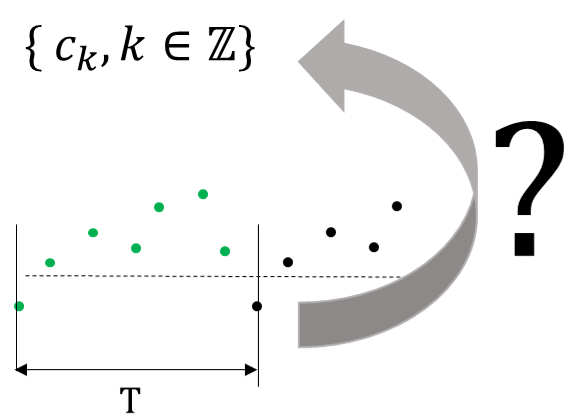
\includegraphics[width=\textwidth]{../Mathematik_2/Bilder/dft_fragestellung_samples_zu_koeffizienten.png}
\end{minipage}
\begin{minipage}{0.7\textwidth}
	Wie l��t sich f�r ein gesampeltes Signal ein Spektrum bestimmen?
\end{minipage}
\end{exabox}

Um diese Frage zu beantworten gehen wir zur�ck zu dem, was wir wissen:
	\begin{itemize}
		\item W�re \(u\) ein stetiges \(T\)-periodisches Signal, so ist das Spektrum diskret und im Allgemeinen unendlich.
		\item Die komplexen Fourierkoeffizienten sind
			\begin{equation}\label{ck_1} c_k = \dfrac{1}{T} \int\limits_{0}^T u(t) \cdot e^{- i\,\omega_k\, t}\,\mathrm d t\,, \quad k\in \mathbb Z\,.\end{equation}
	\end{itemize}

\subsection{Diskrete Fourierkoeffizienten}

Nehmen wir an, dass wir eine \(T\)-periodische Funktion \(u\) im Intervall \([ 0,T) \) in gleichm��igem zeitlichen Abstand abtasten. Die Menge an resultierenden Messpunkte nennt man Samples. Ein Sample besteht aus dem Aufnahmezeitpunkt und dem Messwert. Liegen \(N\) Messpunkte vor, dann kann man sie nummerieren und wie folgt beschreiben:
\[ \begin{array}{rcl}  n& =&0,\cdots,N-1: \\ \textnormal{Sample Nummer } n &:&  \left( t_n, u_n\right) \quad \textnormal{mit} \quad \begin{cases} t_n &= n\cdot h\,, \quad h =\dfrac{T}{N}\,, \\ u_n &= u(t_n)\,. \end{cases} \end{array} \]
Mit den \(N\) Samples kann man die Integrale \eqref{ck_1} zwar nicht exakt, aber n�herungsweise berechnen [approximieren], beispielsweise durch die einfachste numerische Integrationsformel: die Rechteckformel.

\vspace{0.2cm}
\begin{center}
	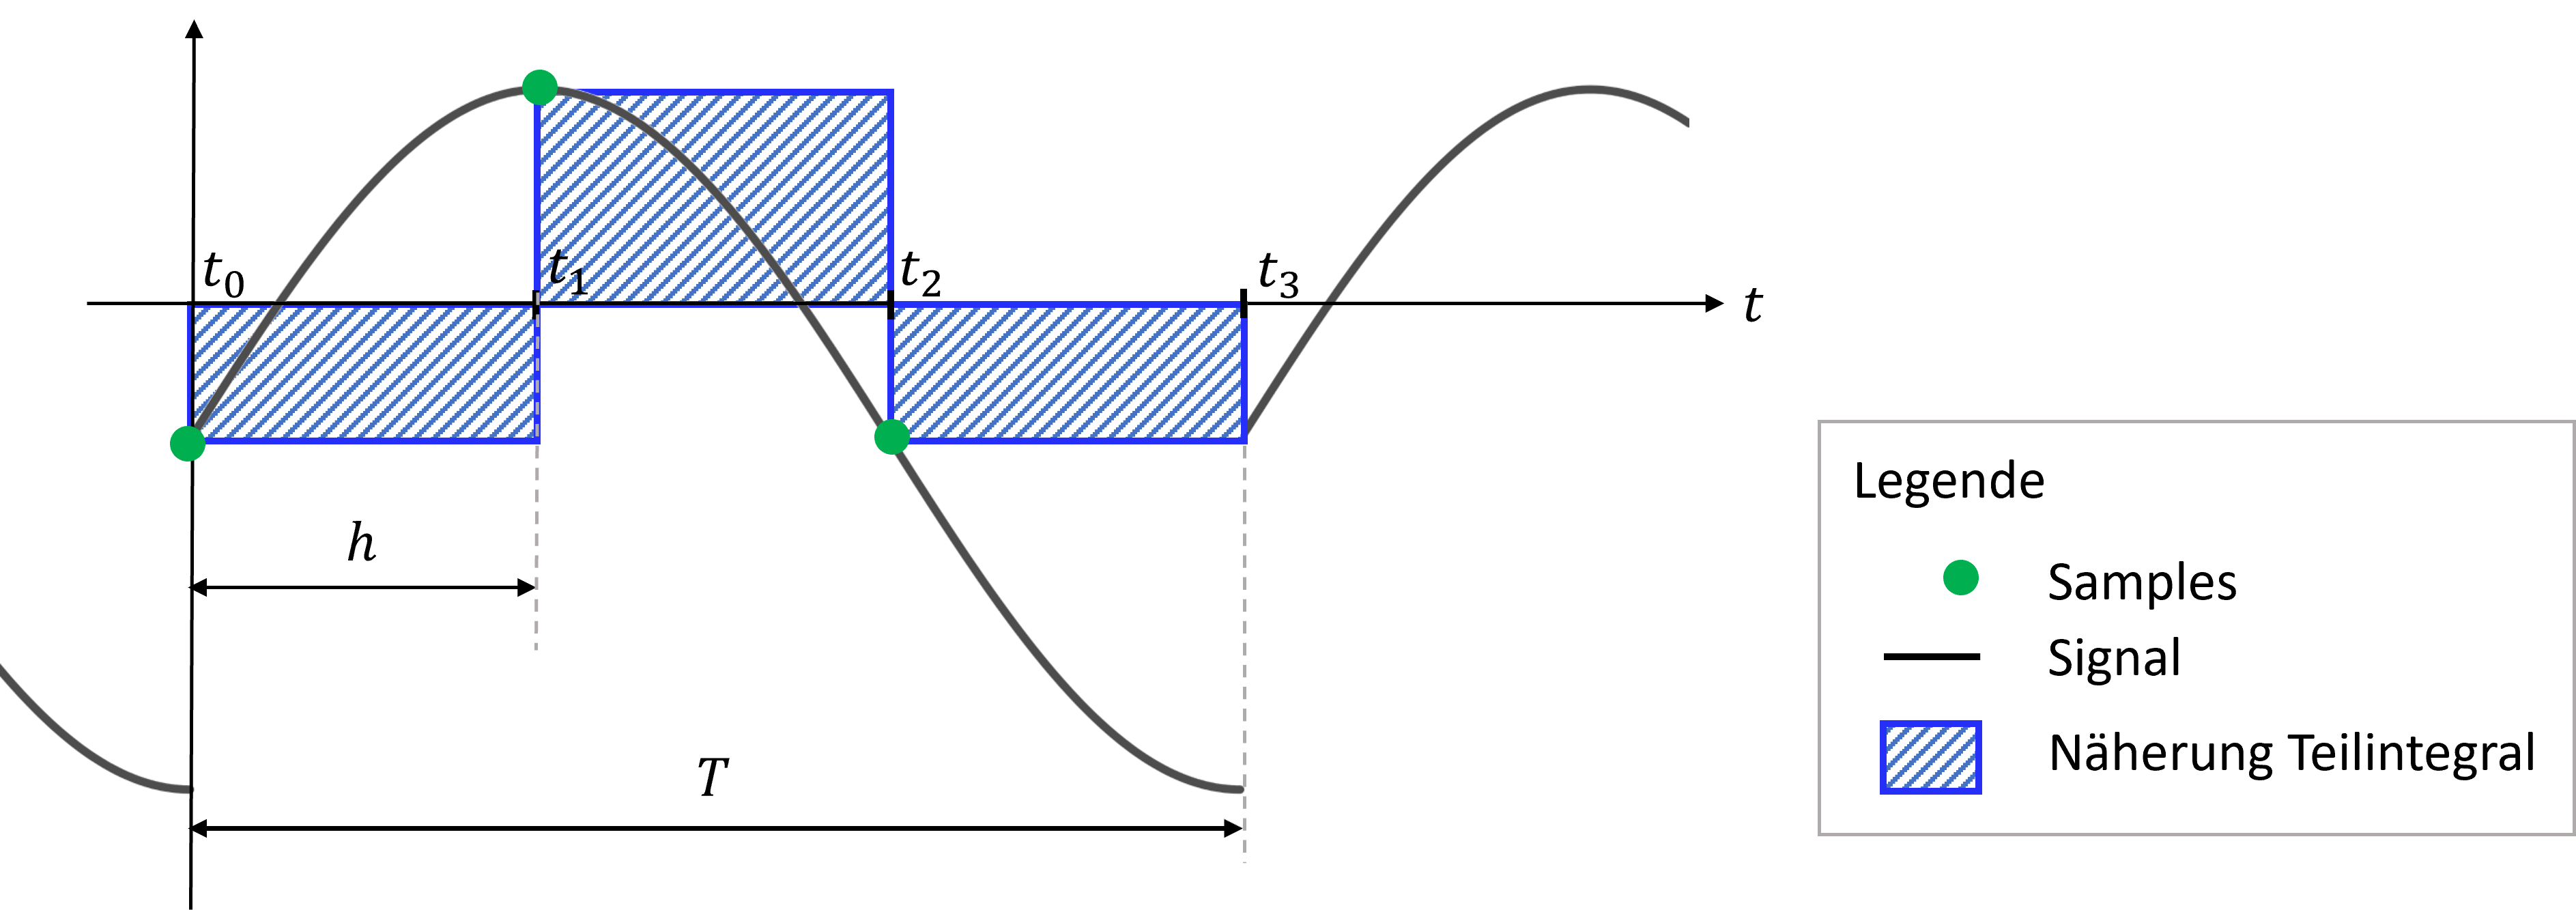
\includegraphics[width=0.8\textwidth]{../Mathematik_2/Bilder/dft_herleitung_rechtecknaeherung_des_integrals.png}
\end{center}
\vspace{0.2cm}

Durch die St�tzstellen \(\{ t_n, \; n=0,\cdots,N\}\) wird das Integrationsintervall in \(N\) Teilintervalle der L�nge \(h\) zerlegt und das Integral �ber jedem Teilintervall \( t \in (t_n, t_{n+1}), \; n=0,\cdots, N-1,\) kann durch ein Rechteck approximiert:
also
		\begin{equation*}
			\begin{array}{l rcl }
				\textnormal{Fourierkoeffizient f�r } k \in \mathbb Z:  & c_k &=& \dfrac{1}{T} \,  \displaystyle{ \int\limits_{0}^T} u(t) \cdot e^{-i\,k\, \omega_0\, t} \,\mathrm d t  \\ \textnormal{Integral zerlegen:} & &=& \dfrac{1}{T} \, \displaystyle{ \sum\limits_{n=0}^{N-1} \int\limits_{t_n}^{t_{n+1}} }  u(t) \cdot e^{-i\,k\, \omega_0\, t} \,\mathrm d t \\[4ex] \textnormal{N�herung durch Rechteck:}  & &\textcolor{blue}{ \approx }& \dfrac{1}{T} \,  \displaystyle{\sum\limits_{n=0}^{N-1}} \textcolor{blue}{u_n \cdot e^{-i \, k \,\omega_0\, t_n} \cdot h} \\ h \textnormal{ ausklammern:} & &&= \dfrac{h}{T} \,  \displaystyle{\sum\limits_{n=0}^{N-1}} u_n \cdot e^{-i \, k \,\omega_0\, t_n} \\[4ex] \omega_0 = \dfrac{2\pi}{T} \mbox{ ersetzen:} & &&= \dfrac{h}{T} \,  \displaystyle{\sum\limits_{n=0}^{N-1}}  u_n \cdot e^{-i \, k \,2\pi/T \, t_n} \\[4ex] T= N\cdot h \mbox{ ersetzen:} & &&= \dfrac{1}{N} \,  \displaystyle{\sum\limits_{n=0}^{N-1}}  u_n \cdot e^{-i \, k \,2\pi/(N\, h) \, t_n}\\[4ex] t_n= n\cdot h\; \mbox{ ersetzen:} & &&=  \dfrac{1}{N} \,  \displaystyle{\sum\limits_{n=0}^{N-1}}  u_n \cdot e^{-i \, k \,2\pi/N \, n} \\[4ex] \textnormal{Potenzregel anwenden:} & &&= \dfrac{1}{N} \, \displaystyle{\sum\limits_{n=0}^{N-1}}  u_n \cdot \left( e^{-i \, 2\pi/N} \right)^{k\cdot n} \,.
		\end{array}
		\end{equation*}

		F�r \(N\) gegebene Samples \( \{ (t_n, u_n)\}_{n=0}^{N-1} \) definieren wir die  \textbf{diskreten Fourierkoeffizienten} wie folgt:\footnote{entsprechend der Definition von Matlab!}
		\[\tilde c_{\textcolor{darkgreen}{k}} : = \sum\limits_{n=0}^{N-1} u_n \cdot \left( \left( \textcolor{blue}{ e^{-i\, \frac{2\pi}{N}} } \right)^{\textcolor{darkgreen}{k}} \right)^{n} = \sum\limits_{n=0}^{N-1} u_n \cdot \left( \left(\textcolor{blue}{ W_N }\right)^{\textcolor{darkgreen}{k}} \right)^{n}\,.\]
		Man k�nnte meinen, dass das Spektrum wie im kontinuierlichen Fall \textcolor{darkgreen}{unendlich} ist, aber das ist nicht so. Bei Vorgabe von \(N\) Samples werden nur maximal \(N\) signifikant verschiedene diskrete Fourierkoeffizienten aus dem Signal detektiert: \[ \tilde c_{\textcolor{darkgreen}{k}} \quad \textnormal{mit} \quad \textcolor{darkgreen}{k=0,\cdots,N-1} \,.\]

		Und warum? Um das zu verstehen, machen wir einen Ausflug in die komplexen Zahlen. Sucht man alle komplexe L�sungen der Gleichung \(z^N=1\), dann findet man, dass es genau \(N\) signifikant verschiedene gibt. Man nennt die L�sungen die \(N\).ten Einheitswurzeln und es sind Potenzen der Zahl \(\textcolor{blue}{ W_N}\):
		\[ \begin{array}{l c rcl} \mbox{Gleichung:} && z^N &=& 1\\[2ex] \mbox{Polardarstellung:} & \Leftrightarrow &  |z|^N \cdot e^{-i\, N\cdot\mathrm{arg}(z)} &=& 1 \cdot e^{-i\, 2\pi \cdot k } \quad \Leftrightarrow  \left\{ \begin{array}{rcl} |z| &=& 1 \,,\\[2ex] \mathrm{arg}(z) &=& -k\,2\pi/N\,. \end{array}\right. \\[3ex] \mbox{L�sungen:} & \Rightarrow & z &=&  \textcolor{blue}{e^{-i\, 2\pi/N \, k}} = \left( \textcolor{blue}{W_N}  \right)^{\textcolor{darkgreen}{k}}, \; \textcolor{darkgreen}{ k=1,\cdots,N-1}\,.  \end{array}\]

	Ist \(N\) beispielsweise \(3\), dann gibt es drei Einheitswurzeln:
\begin{exabox}{Die dritten Einheitswurzeln}{ }
\begin{minipage}{0.35\textwidth}
		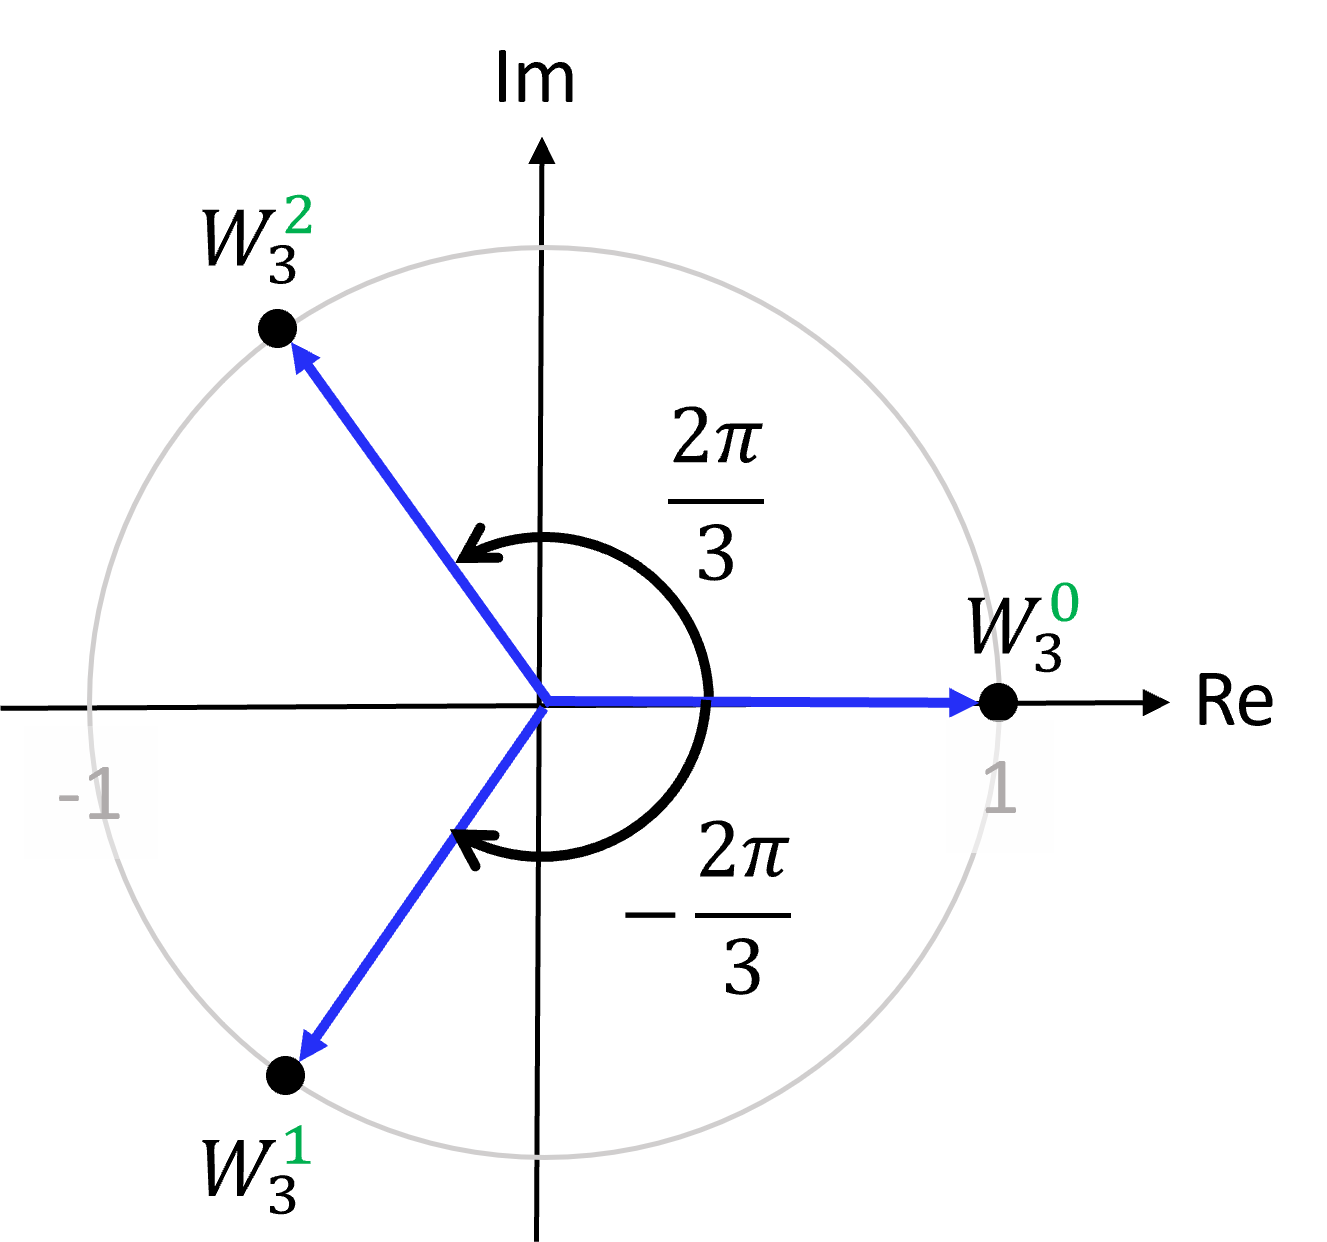
\includegraphics[width=\textwidth]{../Mathematik_2/Bilder/dft_dritte_einheitswurzeln.png}
\end{minipage}
\begin{minipage}{0.65\textwidth}
	\begin{itemize}
		\item Definiere \(W_3 = e^{-i\, \frac{2\pi}{3}} \)
		\item Jede ganzzahlige \textcolor{darkgreen}{Potenz} von \(W_3\) l�st die Gleichung \( z^3 = 1\).
		\item Die Zahlen \(\left( W_3\right)^{\textcolor{darkgreen}{k}}\) liegen auf dem Einheitskreis im Abstand von \(\dfrac{2\pi}{3}\) gleichm��ig verteilt.
		\item F�r \(\textcolor{darkgreen}{k=0,1,2}:\) erhalten wir
			\[ \left\{ \begin{array}{rcl} \left( W_3\right)^0 &=& 1\,, \\ \left( W_3\right)^1 &=& e^{-i\, \frac{2\pi}{3} \cdot 1} \\ \left( W_3\right)^2 &=& e^{-i\, \frac{2\pi}{3} \cdot 2} \, \widehat{=} \, e^{i\, \frac{2\pi}{3}}\,. \end{array} \right. \]
			\item F�r \(k\geq 3\) bzw. \(k<0\) setzt eine Periodizi�t ein: die Werte wiederholen sich zyklisch.
		\end{itemize}
\end{minipage}
\end{exabox}
\bigskip


Es gibt also nur \(N\) unterschiedliche Zahlen der Bauart \( W_N^k\) und genau die lassen sich in der Berechnungsformel f�r die diskreten Fourierkoeffizienten identifizieren:
\[\tilde c_{\textcolor{darkgreen}{k}} : = \sum\limits_{n=0}^{N-1} u_n \cdot \left( \left( \textcolor{blue}{ e^{-i\, \frac{2\pi}{N}} } \right)^{\textcolor{darkgreen}{k}} \right)^{n} = \sum\limits_{n=0}^{N-1} u_n \cdot \left( \textcolor{blue}{W_N}^{\textcolor{darkgreen}{k}} \right)^{n}\,, \quad \textcolor{darkgreen}{ k=0,\cdots,N-1 }\,.\]

\begin{theorembox}{Diskrete Fouriertransformation}{ }
\begin{minipage}{0.4\textwidth}
		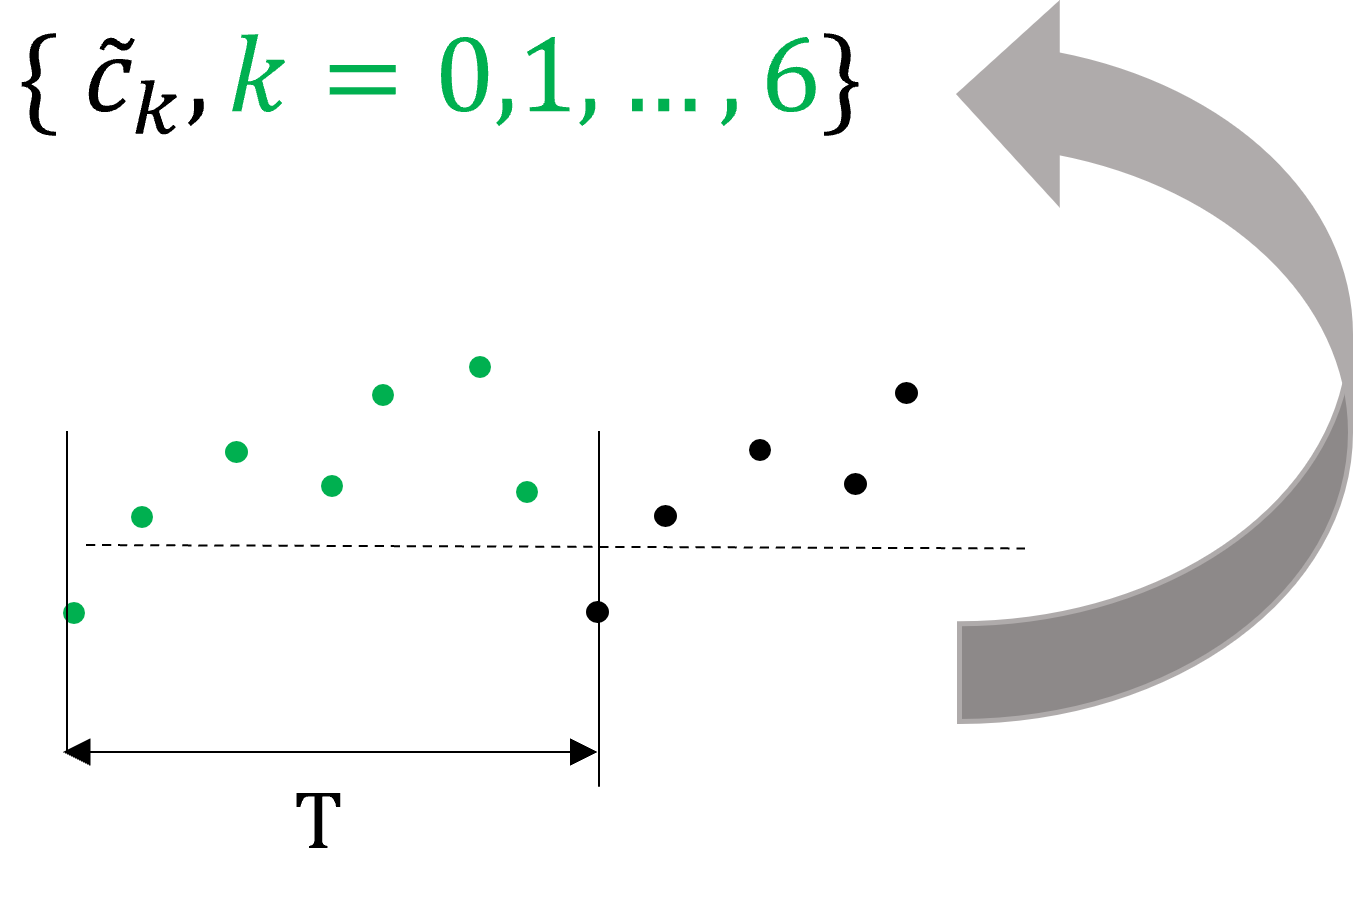
\includegraphics[width=\textwidth]{../Mathematik_2/Bilder/dft_samples_zu_diskreten_koeffizienten.png}
\end{minipage}
\begin{minipage}{0.6\textwidth}
	\begin{itemize}
		\item Es liegen \(N\) Samples vor.
		\item Das Spektrum umfasst \(N\) Fourierkoeffizienten:  \[ \tilde c_k =  \sum\limits_{n=0}^{N-1} u_n \cdot W_N^{k\,n}\,,\; k=0,\cdots,N-1\,.\]
	\end{itemize}
\end{minipage}
\end{theorembox}

\subsection{Diskrete Fouriertransformationen}

\vspace{0.4cm}
Die diskrete Fouriertransformation [DFT] lautet:

\begin{equation}\label{MA2-dft}
\mbox{DFT}: \left\{ u_n,\, n=0,\cdots,N-1\right\} \mapsto  \left\{ \tilde c_k, k=0,\cdots,N-1\right\}, \; \tilde c_k = \sum\limits_{n=0}^{N-1} u_n \cdot W_N^{k\,n} \,. \end{equation}

Bei gegebener DFT (gegebenem Spektrum) l�sst sich ein Fourierpolynom definieren. Das Fourierpolynom ist ein periodisches Signal im Zeitbereich mit Periode \(T = N\cdot h\):
\begin{equation}\label{diskretes_fourier_polynom}
	\mbox{Fourier-Synthese}: \; \left\{ \tilde c_k,\, k=0,\cdots,N-1\right\} \mapsto  g(t) = \dfrac1N \cdot \sum\limits_{k=0}^{N-1} \tilde c_k\cdot  e^{i \,\omega_k \, t }\,, \quad \omega_k = k\cdot \dfrac{2\pi}{T}\,.
\end{equation}
Das Fourierpolynom \(g\) \textbf{interpoliert} die gegebenen \(N\) Samples und das bedeutet\marginpar{{\small Aufgabe}} \[\mbox{Interpolationseigenschaft:} \quad g(t_n) = u_n \; \textnormal{f�r alle } n=0,\cdots,N-1\,. \] Die Interpolationseigenschaft l�sst sich auch wie folgt lesen: eine DFT definiert ein Fourierpolynom \(g\), aus dem man die Messwerte im Zeitbereich generieren oder zur�ckgewinnen kann. Es ergibt sich die Umkehrabbildung zur DFT \eqref{MA2-dft}, man nennt sie die inverse Diskrete Fouriertransformation [iDFT]: \[\begin{array}{l rcl} \mbox{Interpolationseigenschaft:} & u_n &=& g(t_n) \\[2ex] t_n \mbox{ in } g \mbox{ einsetzen:} & &=& \dfrac{1}{N} \cdot \sum\limits_{k=0}^{N-1}\tilde c_k\cdot  e^{i\, k \,\frac{2\pi}{T} \,  t_n} \\[2ex] t_n=n\cdot \frac{T}{N} \mbox{ ersetzen:} & &=& \dfrac1N \cdot \sum\limits_{k=0}^{N-1} \tilde c_k \cdot  e^{i \,\frac{2\pi}{T} \, k \, n \cdot \frac{T}{N} } \\ \mbox{vereinfachen:} & &=&  \dfrac1N \cdot \sum\limits_{k=0}^{N-1} \tilde c_k \cdot \left( \textcolor{blue}{ e^{-i \, \frac{2\pi}{N} }} \right)^{-k \, n } \\ W_N \mbox{ identifizieren:} &  &=&  \dfrac1N \cdot \sum\limits_{k=0}^{N-1} \tilde c_k \cdot \textcolor{blue}{ W_N}^{-k\, n }\,. \end{array} \]

\begin{theorembox}{Inverse Diskrete Fouriertransformation}{ }
\begin{minipage}{0.4\textwidth}
		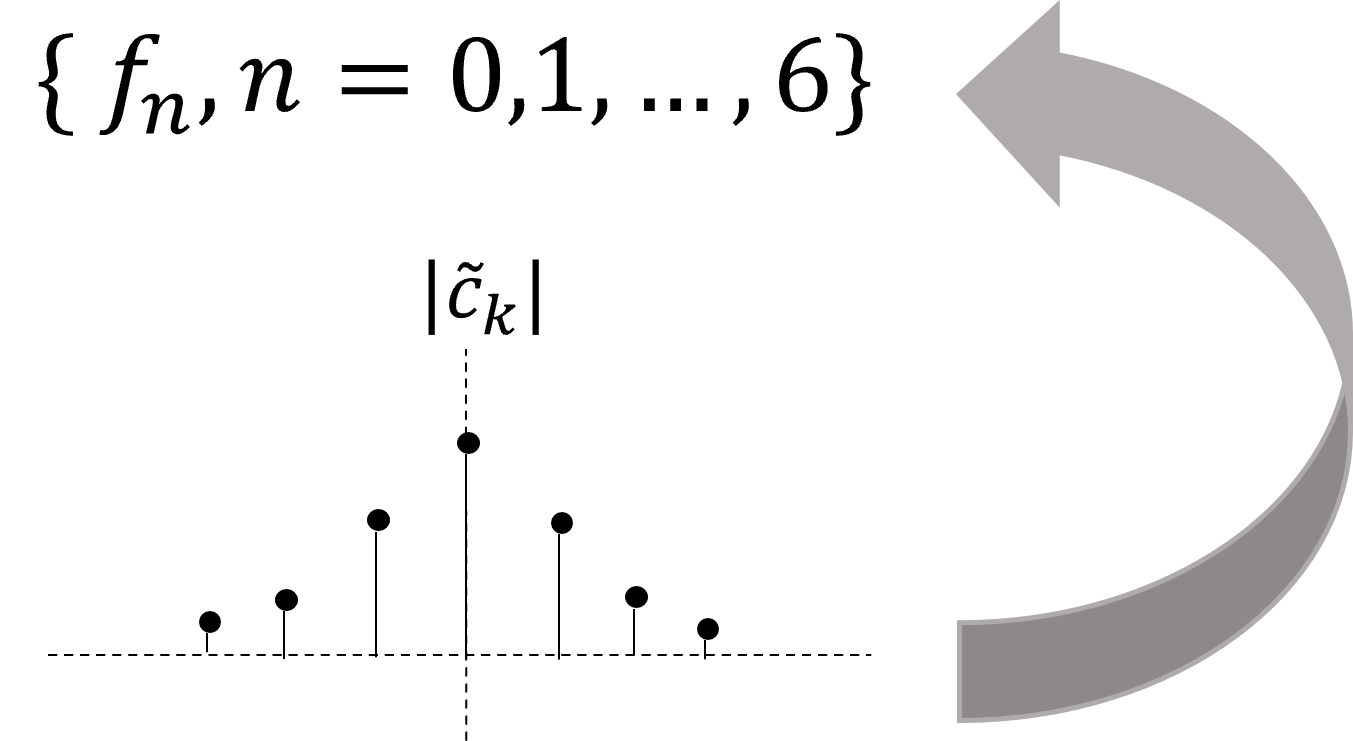
\includegraphics[width=\textwidth]{../Mathematik_2/Bilder/idft_koeffizienten_zu_samples.png}
\end{minipage}
\begin{minipage}{0.6\textwidth}
	\begin{itemize}
		\item Es liegt eine DFT mit \(N\) Fourierkoeffizienten vor.
		\item Es gibt hierzu \(N\) eindeutige Samples:
		\[ u_n = \dfrac{1}{N}\cdot \sum\limits_{k=0}^{N-1} \tilde c_k \cdot W_N^{-k\,n}\,,\; n=0,\cdots,N-1\,.\]
	\end{itemize}
\end{minipage}

\vspace{0.4cm}

Die inverse diskrete Fouriertransformation [iDFT] lautet:

\begin{equation}\label{MA2-idft}
\mbox{iDFT}: \left\{ \tilde c_k, k=0,\cdots,N-1\right\} \mapsto \left\{ u_n,\, n=0,\cdots,N-1\right\}, \; u_n = \dfrac{1}{N}\cdot \sum\limits_{k=0}^{N-1} \tilde c_k \cdot W_N^{-k\,n} \,. \end{equation}
\end{theorembox}

Die iDFT ist die inverse der DFT, ensprechend bildet sie vom Frequenzbereich in den Zeitbereich ab. Die Verbindung zwischen den beiden Welten ist das interpolierende Fourierpolynom:

\begin{exabox}{DFT-Fourierpolynom-iDFT}{ }
	\begin{center}
		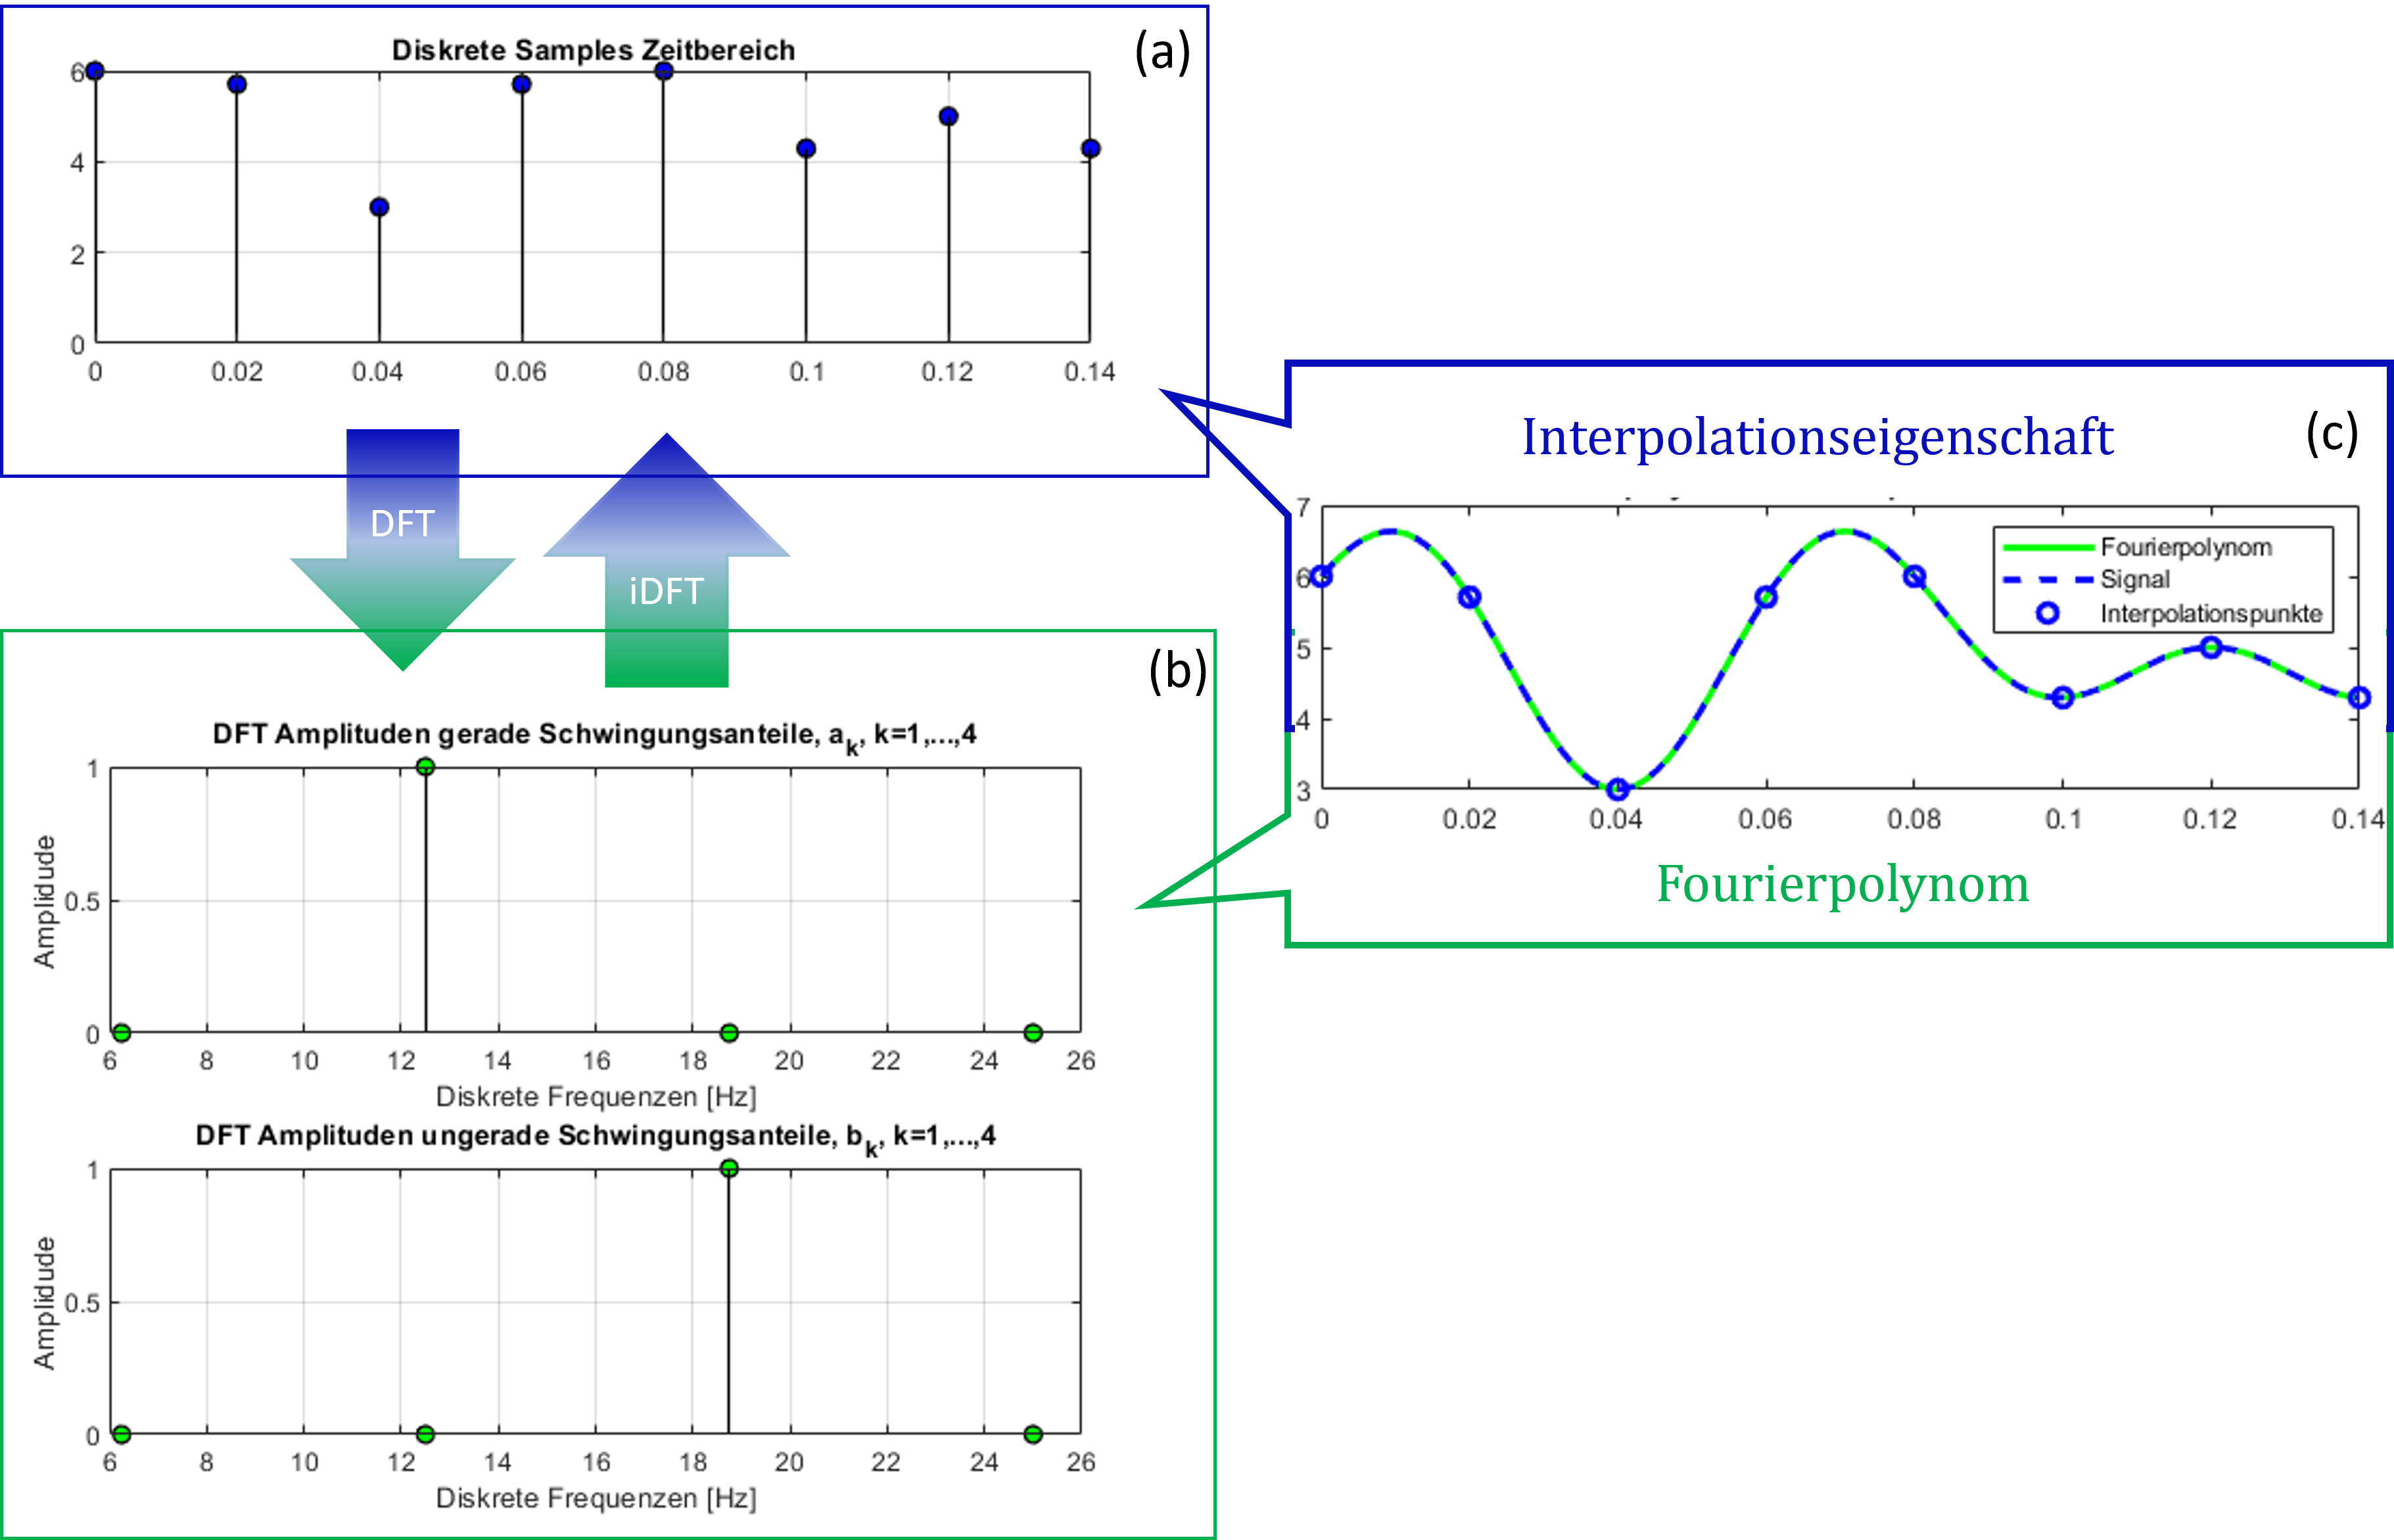
\includegraphics[width=\textwidth]{../Mathematik_2/Bilder/dft_idft_und_interpolierendes_fourierpolynom.png}
	\end{center}
	\begin{itemize}
		\item[(a)] Das Bild zeigt die Samples im Zeitbereich.
		\item[(b)] Das Bild zeigt die DFT mit reellen Koeffizienten: \(a_k, 1\leq k \leq 4\) und \(b_k, \; 1\leq k \leq 4\).
		\item[(c)] Das Bild zeigt das resultierende Fourierpolynom, das Ausgangssignal und die Samples.
	\end{itemize}
	\begin{itemize}
		\item[(a)] \(\Rightarrow\) (b) Berechnung des Frequenzspektrums durch DFT.
		\item[(b)] \(\Rightarrow\) (a) Berechnung der Messwerte durch iDFT.
		\item[(c)] \(\Rightarrow\) In dem Beispiel detektiert die DFT alle im Signal vorhandenen Frequenzen exakt: \(f \equiv g\).
	\end{itemize}
\end{exabox}
\bigskip

{\noindent \textbf{Bemerkungen:}}
	\begin{itemize}
		\item Welche diskreten Kreisfrequenzen f�r gegebene Samples detektiert werden k�nnen, ist a-priori bekannt.
\item Es gibt keine einheitliche Definition f�r DFT und iDFT bez�glich der Skalierung. Genauso wie bei der Fouriertransformation kann man die Formel auch symmetrisieren.
		\item Man kann anstatt der komplexen Fourierkoeffizienten die reellen Fourierkoeffizienten \(a_k\) und \(b_k\) und entsprechend das reelle Fourierpolynom betrachten.
\end{itemize}

\subsection{DFT als lineare Abbildung}

Die Diskrete Fouriertransformation ist die Abbildung, die dem Vektor \(\vec u\) der diskreten Signaldaten \(\vec u\in \mathbb C^N\) im Zeitbereich den Vektor der Fourierkoeffizienten \(\vec c\in\mathbb C^n\) im Frequenzbereich zuordnet. \[ \mathrm{DFT}: \mathbb C^N\to \mathbb C^N, \vec u \mapsto \vec c\,. \] Schauen wir uns die Berechnung eines einzelnen Koeffizienten \(\tilde c_k\) an, so wird klar, dass die Fourierkoeffizienten das Ergebnis einer Matrix-Vektor Multiplikation sind:\marginpar{{\small Aufgabe}}
\begin{eqnarray*}
	\tilde c_k &=& \sum\limits_{n=0}^{N-1} W_N^{k\, n} \cdot u_n = \left( W_N^{k\cdot 0}, W_N^{k\cdot 1}, \cdots, W_N^{k\cdot (N-1)} \right) \left( \begin{array}{c} u_0\\u_1 \\\vdots \\ u_{N-1} \end{array}\right)\\[2ex]
	&\Rightarrow& \left( \begin{array}{c} \tilde c_0 \\ \tilde c_1 \\ \vdots \\ \tilde c_{N-1} \end{array}\right) = \left( \begin{array}{llll} W_N^{0} & W_N^{0} & \cdots & W_N^{0} \\ W_N^{0} & W_N^{1} & \cdots & W_N^{(n-1)} \\ \vdots & \vdots & \ddots & \vdots \\ W_N^{0} & W_N^{(N-1)} & \cdots & W_N^{(N-1)^2} \end{array}\right) \left(\begin{array}{c} u_0 \\u_1 \\ \vdots \\u_{N-1}\end{array}\right)\,.
\end{eqnarray*}
Die DFT ist also die folgende, \textbf{lineare Abbildung}
\[
\textnormal{DFT:}\quad \mathbb C^N \to \mathbb C^N, \; \vec u \mapsto \vec c = T_N \vec u\,, \quad (T_N)_{kl} = \left( W_N\right)^{kl}, \; k,l=0,\cdots,N-1\,.
\]

\noindent \textbf{Bemerkungen:}
\begin{itemize}
	\item \(T_N\) nennt man Matrix der Diskreten Fouriertransformation der Ordnung \(N\).
	\item \(T_N\) ist regul�r und das hei�t, dass durch die Multiplikation \(T_N \, \vec u\) ein Basiswechsel passiert.
	\item Die inverse Matrix \(T_N^{-1}\) ist die Matrix der inversen Diskreten Fouriertransformation der Ordnung \(N\).
\end{itemize}


Die DFT Matrix \(T_2\) lautet \[ T_2 = \left( \begin{array}{cc} W_2^0  & W_2^0 \\  W_2^0 & W^1_2 \end{array}\right) = \left( \begin{array}{cc} 1 & 1 \\ 1 & -1 \end{array}\right)\,.\] F�r \(2\) Samples, also ein Messsignal \(\vec u\in \mathbb C^2\), ist die DFT: \[ \left(\begin{array}{c} \tilde c_0 \\ \tilde c_1\end{array}\right) = \left( \begin{array}{cc} 1 & 1 \\ 1 & -1 \end{array}\right)\, \left( \begin{array}{c} u_0 \\ u_1 \end{array}\right) \,. \]

Die DFT Matrix \(T_4\) lautet \[ T_4 = \left( \begin{array}{cccc} W_4^0 &  W_4^0 & W_4^0  & W_4^0 \\ W_4^0 & W^1_4 & W_4^2 & W_4^3  \\ W_4^0 & W_4^2 & W_4^4 & W_4^6  \\   W_4^0  & W_4^3 & W_4^6 & W_4^9\end{array}\right) = \left( \begin{array}{cccc} 1 & 1 & 1 & 1 \\ 1&-i&-1&i \\ 1 & -1 & 1 & -1  \\ 1 & i & -1 & -i\end{array}\right) \]

F�r \(4\) Samples, also ein Messsignal \(\vec u\in \mathbb C^2\), ist die DFT:
\[
		\vec c  = \left( \begin{array}{rrrr} 1 & 1 & 1 & 1 \\ 1& -i& -1 & i \\ 1 & -1 & 1 & -1  \\ 1 & i & -1 & -i \end{array}\right) \, \left( \begin{array}{c} {u_{0}} \\ u_{1}\\ {u_{2}} \\u_{3} \end{array}\right)\]


%\subsection{Vokabular}
%Im Kontext von Signalverarbeitung gibt es eine Fachsprache und es ist wichtig, dass man sie kennt. Beispielsweise spricht man eigentlich nicht mehr von der Schrittweite \(h\) [\(\Delta t\)], sondern bezieht alle Gr��en auf die Abtastrate und die Zeitspanne der Aufzeichnung.
%
%\vspace{0.5cm}
%\begin{table}[H]
%\centering
%\begin{tabularx}{\textwidth}{l | c| X |c}
%	Symbol & Name &  Beschreibung & Regel\\\midrule
%\(u_s\) & Abtastrate & \vspace{-0.5cm} \begin{itemize} \item Die Abtastrate  [sampling frequency] ist die Anzahl der pro Sekunde aufgezeichneten Signalwerte. \item \(u_s\) ist gerade das Reziproke der Schrittweite \(h\) [sampling interval]: \( h = \dfrac{1}{u_s} \; \mathrm{s}\,.\) \end{itemize} & \( u_s: \# \textnormal{ Samples pro Seckunde } [\mathrm{Hz}]\) \\\midrule
%\(N\) & Anzahl Samples  &\vspace{-0.5cm} \begin{itemize} \item  \(N\) ist die Gesamtanzahl der Messwerte, die man f�r die DFT zur Verf�gung hat. \end{itemize} & \( N: \#  \textnormal{ Samples } \) \\\midrule
%\(t_N\) & Zeitspanne & \vspace{-0.5cm} \begin{itemize} \item \(t_N\) ist  die L�nge des Zeitintervalls [sample length], in dem Messwerte aufgezeichnet werden. \item \(t_N\) ist die Periode des aus der DFT resultierenden Fourierpolynoms \(g\) \end{itemize} & \( t_N = \dfrac{N}{u_s}\; [\mathrm{s}]\)
%\end{tabularx}
%\end{table}
%
%
%Die Frequenzen, die eine DFT detektieren wird, sind bekannt, sobald man die Abtastrate \(u_s\) und die Zeitspanne \(t_N\) kennt. Man gibt oft die gr��te und die kleinste dieser Frequenzen an.\marginpar{{\small Aufgabe}}
%
%\vspace{0.5cm}
%\begin{table}[H]
%\centering
%\begin{tabularx}{\textwidth}{l | c| X |c}
%	Symbol & Name &  Beschreibung & Regel\\\midrule
%	\(u_{\max}\) & Nyquist Frequenz & \vspace{-0.5cm} \begin{itemize} \item \(u_{\max}\) ist die gr��te Freqzenz, die aus einem gesampleten Signal rekonstruiert werden kann. \item Die Nyquist Frequenz ist die H�lfte der Abtastrate.\end{itemize} & \( u_{\max} = \dfrac{u_s}{2} \; \mathrm{Hz}\) \\\midrule
%	\(u_{\min}\) & Minimale Frequenz &\vspace{-0.5cm}  \begin{itemize} \item \(u_{\min}\) ist die kleinste Frequenz, die rekonstruiert werden kann. \item Periodizit�ten des Signals, die sich unterhalb der Schrittweite \(h\) abspielen, k�nnen von einer DFT nicht erfasst werden.\end{itemize} & \( u_{\min} = \dfrac{1}{t_N} \)
%\end{tabularx}
%\end{table}
%
%\begin{defbox}{ Vokabular }{ }
%Nehmen wir beispielsweise an, dass wir von einem Signal \(n=100\) Samples mit einer Abtastrate von \(u_s = 1000\,\mathrm{Hz}\) aufzeichnen. Dann gilt
%\[
%	\begin{array}{l rcl}
%		\textnormal{Schrittweite:} & h &=& \dfrac{1}{u_s} = 0.001 \, \mathrm{s/Samples} \,,\\[2ex]
%		\textnormal{Zeitspanne:} & t_N &=& \dfrac{n}{u_s} = 0.1 \, \mathrm{s} \,,\\[2ex]
%		\textnormal{Frequenzinkrement:} & \Delta f &=& \dfrac{u_s}{N} =  10 \, \mathrm{Hz} \,,\\[2ex]
%		\textnormal{Nyquist Frequenz: } & u_{\max} &=& \dfrac{u_s}{2} = 500 \, \mathrm{Hz} \,,\\[2ex]
%	\textnormal{Minimale Frequenz: }  & u_{\min} &=& \dfrac{1}{t_N} = 10 \, \mathrm{Hz} \,.
%\end{array}
%\]
%\end{defbox}
%
 \newpage % 11 Diskrete Fouriertrafo
%\setcounter{exercise}{0} 
\ifintegriereaufgaben

\section*{Diskrete Fouriertransformation}\label{MA2-diskrete-fouriertransformation-aufgaben}
Regeln und Beispiele, die zur Bearbeitung der Aufgaben hilfreich sind, finden Sie im Skript\wennreferenzvorhanden{MA2-diskrete-fouriertransformation}{ (Abschnitt \abschnittsverweis{MA2-diskrete-fouriertransformation})} und, falls Sie nicht weiterkommen, schauen Sie \hyperref[MA2-diskrete-fouriertransformation-loesungen]{hier}.
\else
\section{Diskrete Fouriertransformation}\label{MA2-diskrete-fouriertransformation-aufgaben}

Regeln und Beispiele zu diesen Aufgaben finden Sie im Skript. Die L�sungen finden Sie \hyperref[MA2-diskrete-fouriertransformation-loesungen]{hier}.
\fi

\begin{exabox}[Orthogonalit�t]
	Bei der Digitalsignal�bertragung werden energiebegrenzte Signale betrachtet. Das Skalarprodukt zweier Signale bzw. die Norm eines Signals sind hierbei wie folgt definiert:
	\begin{eqnarray*}
		\langle s_i, s_k\rangle &=& \int\limits_{-\infty}^{\infty} s_i(t) \cdot s_k(t) \, \mathrm{d}t\,,\\[1ex]
		\|s\| &=& \sqrt{\langle s,s \rangle}\,.
	\end{eqnarray*}
	Betrachten Sie die folgenden drei energiebegrenzten Signale:
	\begin{center}
	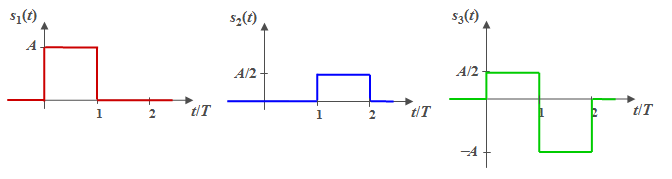
\includegraphics[width=0.7\textwidth]{../Mathematik_2/Bilder/dft_rechtecksignale_linearkombination.png}
\end{center}
	\begin{itemize}
		\item[(a)] Wie lauten die Abbildungsvorschriften der Signale $s_1, s_2$ und $s_3$?
		\item[(b)] Berechnen Sie die Normen der Signale $s_1$ und $s_2$.
		\item[(c)] Konstruieren Sie aus den Signalen $s_1$ und $s_2$ ein Orthonormalsystem.
		\item[(d)] Zerlegen Sie das Signal $s_3$ bez�glich des Orthonormalsystems und bestimmen Sie die vektoriellen Repr�sentanten der Ausgangssignale bez�glich des Orthonormalsystems.
	\end{itemize}
\end{exabox}

\begin{exabox}[�quivalenz reelle und komplexe Fourierreihe]
	Zeigen Sie, dass es zur komplexen Fourierreihe eine �quivalente reelle Darstellung gibt und geben Sie an, wie sich die Koeffizienten ineinander �berf�hren lassen. Hinweis: Benutzen Sie die Eulersche Identit�t.%  \( e^{i\,k\omega t} =  \cos(k \omega_0 t) + i \sin(k \omega_0 t) \,. \)
\end{exabox}

\begin{exabox}[Matlab Funktion: Fourierreihe Rechtecksignal]
%	16.6 p.427
	Die Stromst�rke in einem elektrischen Stromkreis verh�lt sich in vielen F�llen wie ein Rechtecksignal. Ein Rechtecksignals ist die periodische Fortsetzung der folgenden Funktion \(f: [0,T) \to f(t)\,,\) wobei

	\[ f(t) = \begin{cases} &A_0, \quad 0\leq t \leq T/2\,,\\ -&A_0, \quad T/2\leq t < T\,. \end{cases} \]

\begin{minipage}{0.5\textwidth}
	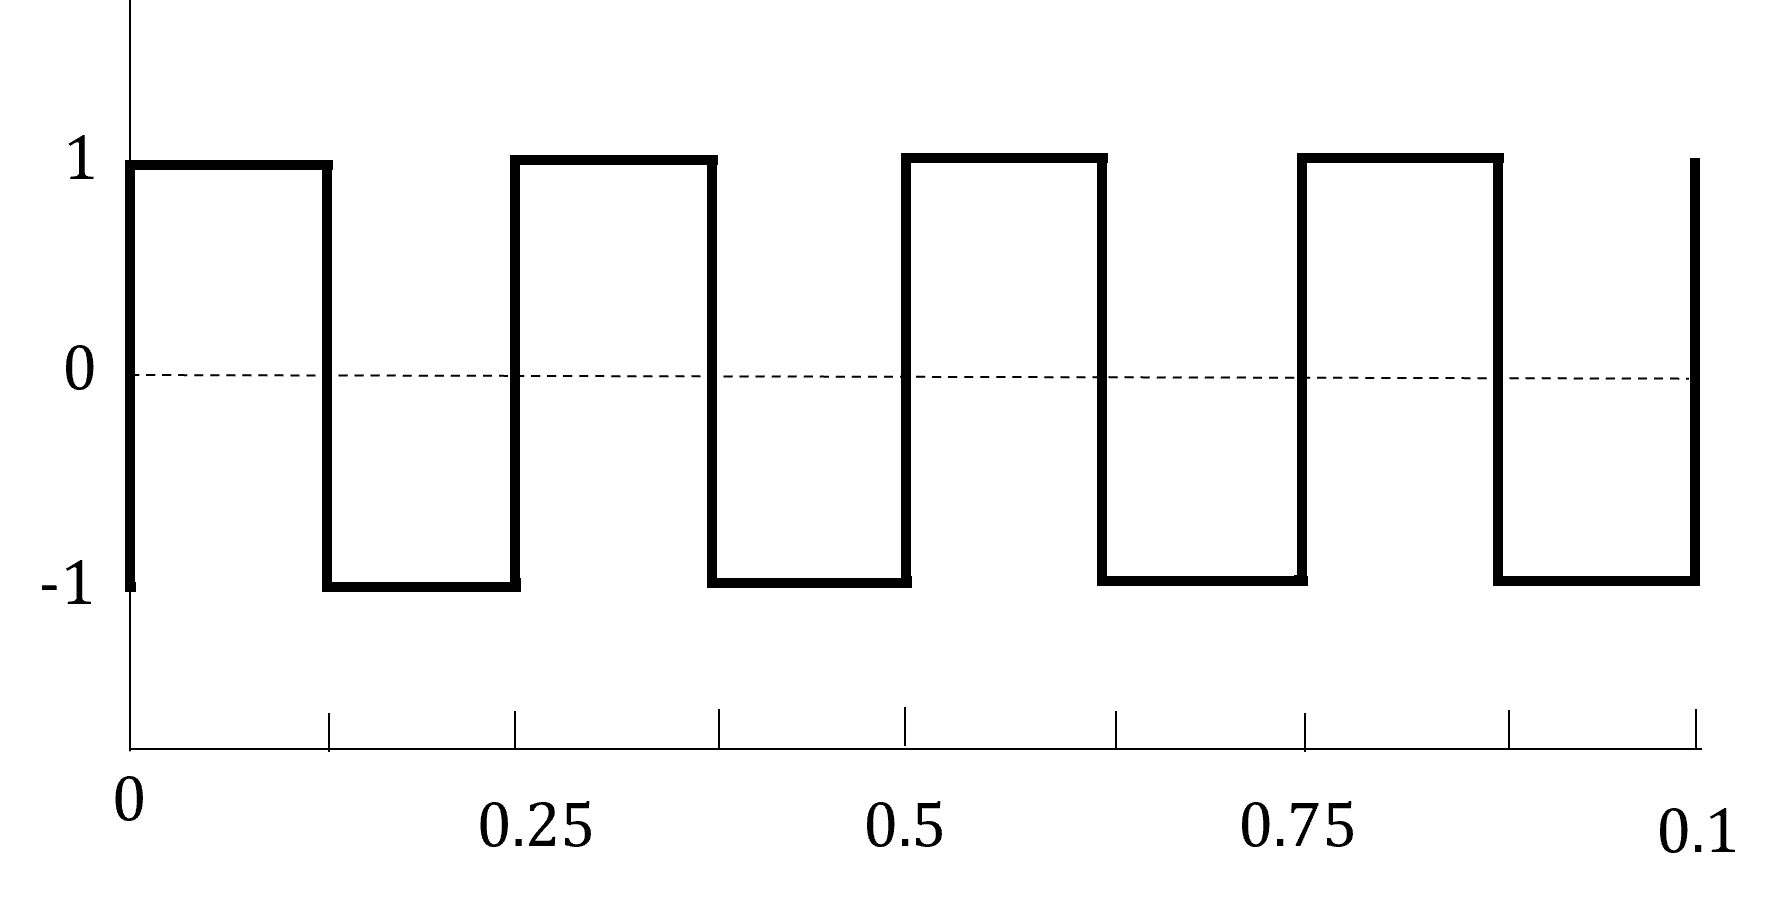
\includegraphics[width=\textwidth]{../Mathematik_2/Bilder/dft_rechtecksignal_wechselndes_vorzeichen.png}
\end{minipage}
\begin{minipage}{0.5\textwidth}
	Das Bild zeigt den Graph von \(f\) f�r \(A_0=1\,, \, T=1/4\):
	\[ f(t) = \begin{cases} &1, \quad 0\leq t \leq 1/8\,,\\ -&1, \quad 1/8\leq t < 1/4\,. \end{cases} \]
\end{minipage}

\begin{itemize}
	\item[(a)] Analysieren Sie die Symmetrie des Signals \(f\) und berechnen Sie anschlie�end die reelle Fourierreihe von \(f\).
	\item[(b)] Schreiben Sie die Matlab Funktion
		\begin{lstlisting}
		function [t,FR] = FourierSquare(A0, T, n)
		\end{lstlisting}
		\(\verb-FourierSquare-\) erh�lt als Eingabedaten die Amplidude \(A_0\), die Periode \(T\) des Rechtecksignals und den Grad \(n\) des gew�nschten Fourierpolynoms. \(\verb-FourierSquare-\) erzeugt ein Bild, auf dem
		\begin{itemize}
			\item die Graphen der ersten \(n\) Terme der Fourierreihe �ber dem Intervall \([0,T)\) abgebildet sind, jede Funktion wird mit d�nner, gestrichelter roter Linie gemalt, und,
			\item der Graph des Fourierpolynoms vom Grad \(n\) mit dicker, schwarzer Linie gemalt (\verb+'k-','linewidth',2+).
		\end{itemize}
\end{itemize}
\end{exabox}

\begin{exabox}[Minimierungsproblem]
	Es sei \(f\) ein \(2\pi\)-periodisches Signal. Zeigen Sie, dass das Fourierpolynom
	\[
	g_n(t) = \dfrac{a_0}{2} + \sum\limits_{k=1}^n a_k \cos(k\cdot t) + b_k \sin(k\cdot t), \quad a_k = \dfrac{1}{\pi} \int\limits_{-\pi}^{\pi} f(t)\cdot \cos(k\cdot t)\,\mathrm{d} t, \; b_k = \dfrac{1}{\pi} \int\limits_{-\pi}^{\pi} f(t)\cdot \cos(k\cdot t)\,\mathrm{d} t\,,\]
	unter allen trigonometrischen Polynomen vom Grad \(n\) den kleinsten Abstand zu \(f\) hat. Das Abstandsma� ist \[ ||f-g||_2 = \sqrt{ \int\limits_{-\pi}^\pi |f(t) - g(t)|^2 \, \mathrm{d} t }\,.\]
\end{exabox}

\begin{exabox}[Interpolationseigenschaft]
	Gegeben sind \(N\) Samples \(\left( t_n, f_n\right), \; n=0,\cdots,N-1,\) eines \(T\)-periodischen Signals \(f\). Zeigen Sie, dass die DFT ein Fourierpolynom definiert, das alle Samples interpoliert.
\end{exabox}

\begin{exabox}[DFT per Hand]
	Nehmen wir an das kontinuierlich gegebene Signal
	\[ f: t\mapsto 5 + 2\cos(2\pi t - \pi/2) + 3\cos(4\pi t) \]
	wird pro Sekunde vier Mal abgetastet.
	\begin{itemize}
		\item[(a)] Bestimmen Sie die Samples, die in einer Sekunde gemessen werden.
		\item[(b)] Bestimmen Sie die diskrete Fourier-Transformation und zeigen Sie, dass sich die diskrete Founier-Transformation als Matrix-Vektor-Multiplikation schreiben l��t.
		\item[(c)] Wie l��t sich das Ergebnis interpretieren?
	\end{itemize}
\end{exabox}

\begin{exabox}[Matlab: Diskrete Fouriertransformation (DT)] % p.428 16.11 standard
	Gegeben ist das Signal \[ f: t\mapsto  \cos\left(2\pi \cdot \dfrac{25}{2} \cdot t\right) + \cos\left( 2\pi \cdot 25 \cdot t\right)\,. \] Generieren Sie \(64\) Samples mit Schrittweite \(\Delta t = 0.01\, \mathrm{s}\).
	\begin{itemize}
		\item[(a)] Bestimmen Sie die Abtastrate \(f_s\), die Zeitspanne der Aufzeichnung \(t_n\), die Nyquist Freqzenz \(f_{\max}\) und die minimale detektierbare Frequenz \(f_{\min}\).
		\item[(b)] Bestimmen Sie mit Hilfe der Matlab Funktion \(\verb-fft-\) die diskrete Fouriertransformation ausgehend von den \(64\) Samples und plotten Sie das Spektrum.
	\end{itemize}
\end{exabox}

\begin{exabox}{Matlab: Experiment: DFT Leck-Effekt}{ } %
	Gegeben sind die folgenden zwei Funktionen
	\[ \begin{array}{rcl}
			f_1: \mathbb R\to \mathbb R,  &t \mapsto \cos(2\pi \, t)\,,\\
			f_2: \mathbb R\to \mathbb R,  &t \mapsto \cos(2\pi/(1.2) \, t)\,.
		\end{array}
	\]
	\begin{itemize}
		\item[(a)] Betrachten Sie das Signal \(f_1\) und generieren Sie \(8\) �quidistante Samples auf dem Intervall \([0,3)\). Bestimmen Sie mit Hilfe der Matlab Funktion \(\verb-fft-\) das periodische Spektrum des diskreten Signals. Illustrieren Sie das Ergebnis der DFT wie folgt:
			\begin{itemize}
				\item Visualisieren Sie das Spektrum, das die DFT liefert mit Hilfe von zwei Bildern:
					\begin{itemize}
						\item[(i)] Zeichnen Sie die Amplituden \(a_k\) in Abh�ngigkeit der diskreten Frequenzen, also \( f_k \mapsto a_k\,, \; k=1,\cdots,4\,.\)
						\item[(ii)] Zeichnen Sie die Amplituden \(b_k\) in Abh�ngigkeit der diskreten Frequenzen, also \( f_k \mapsto b_k\,, \; k=1,\cdots,4\,.\)
						\end{itemize}
					\item Visualisieren Sie die G�te der DFT, in dam Sie das Signal \(f_1\), das durch die DFT definierte Fourierpolynom \(g_1\) und die Samples zusammen im Intervall \([0,3]\) zeichnen.
			\end{itemize}
		\item[(b)] Betrachten Sie nun das Signal \(f_2\) und generieren Sie \(8\) �quidistante Samples auf dem Intervall \([0,3)\). Bestimmen Sie mit Hilfe der Matlab Funktion \(\verb-fft-\) das periodische Spektrum des diskreten Signals.
			\begin{itemize}
				\item Visualisieren Sie das Spektrum, das die DFT liefert mit Hilfe von zwei Bildern:
					\begin{itemize}
						\item[(i)] Zeichnen die Amplituden \(a_k\) in Abh�ngigkeit der diskreten Frequenzen, also \( f_k \mapsto a_k\,, \; k=1,\cdots,4\,.\)
						\item[(ii)] Zeichnen die Amplituden \(b_k\) in Abh�ngigkeit der diskreten Frequenzen, also \( f_k \mapsto b_k\,, \; k=1,\cdots,4\,.\)
						\end{itemize}
					\item Visualisieren Sie die G�te der DFT, in dam Sie das Signal \(f_2\), das durch die DFT definierte Fourierpolynom \(g_2\) und die Samples zusammen im Intervall \([0,3]\) zeichnen.
			\end{itemize}
		\item[(c)] Wie l��t sich erkl�ren, dass die beiden Spektren so unterschiedlich sind?
	\end{itemize}
\end{exabox}

\begin{exabox}[Matlab: Experiment: DFT gest�rte Daten] % p.428 16.12 noise
	Betrachten Sie das folgende periodische Signal
	\[ f: \mathbb R\to \mathbb R,  t\mapsto \cos(10\cdot t) + \sin(3\cdot t) \]
	und generieren Sie \(64\) �quidistante Samples auf dem Intervall \([0,2\pi)\). Ver�ndern Sie die exakten Daten durch Hinzuaddieren einer Zufallszahl mit Hilfe von \verb-randn-. Bestimmen Sie mit \verb-fft- die DFT der gest�rten Daten und plotten Sie das Ergebnis.
\end{exabox}

 \newpage  % VPL Matlab Experimente
\setcounter{def}{0} \setcounter{satz}{0} \setcounter{exa}{0} \section{Fourier-Transformation (+)}\label{MA2-fouriertransformation}

\begin{table}[H]
  \centering
  \begin{tabularx}{\textwidth}{@{}>{\raggedright\arraybackslash}X r@{}}
    \toprule
    \multicolumn{2}{c}{\textbf{�bersicht �ber Lernziele und Voraussetzungen}} \\
    \midrule
    \textbf{Lernziele} & \\[.5\normalbaselineskip]
    \tabitem die Fourier-Transformierte einer absolut integrierbaren Funktion berechnen & \\
    \tabitem grundlegende Eigenschaften der Fourier-Transformation anwenden & \\
    \tabitem die Bedeutung der Fourier-Transformation im Frequenzraum erl�utern & \\[.5\normalbaselineskip]
    \midrule
    \textbf{Voraussetzungen} &  \\[.5\normalbaselineskip]
    \tabitem uneigentliche Integrale berechnen k�nnen & \abschnittsverweis{MA2-integration}  \\
    \tabitem Grenzwerte sicher bilden k�nnen & \abschnittsverweis{MA1-grenzwerte-von-folgen-und-funktionen}  \\[.5\normalbaselineskip]
    \bottomrule
  \end{tabularx}
\end{table}

\noindent \ifintegriereaufgaben Die �bungsaufgaben zum Thema finden Sie \hyperref[MA2-fouriertransformation-aufgaben]{hier}.
\vspace{0.3cm}
\hrule
\fi

\subsection{Fragestellung}

Kann man auch f�r Funktionen, die nicht periodisch, sind ein Spektrum finden? Wenn ja, wie sieht das Spektrum aus und wie berechnet man es? Mit diesen Fragen werden wir uns in diesem Abschnitt besch�ftigen. Die Antwort auf die Frage lautet "\,ja, kann man"\, und das Ergebnis ist eine Funktion, die sogenannte Fourier-Transformierte.

\subsection{Definition}

Betrachten wir eine Funktion \(f: \mathbb R \to \mathbb C, t \mapsto f(t)\), die nicht periodisch ist, aber f�r die gilt:
\begin{itemize}
	\item[(a)] $f$ ist stetig differenzierar und
	\item[(b)] \(f\) ist absolut integrierbar  \(\quad \displaystyle \int\limits_{-\infty}^\infty |f(t)|\,\mathrm{d}t < \infty \,. \)
\end{itemize}

Mit dem folgenden Trick n�hern wir uns langsam der Frage nach dem Spektrum von \(f\):
\begin{enumerate}
	\item Wir w�hlen eine positive, reelle Zahl $T>0$ und fixieren das Intervall $\left(-\frac{T}{2}, \frac{T}{2}\right)$.
	\item Wir definieren eine periodische Funktion $g$, \(g(t) = g(t+T)\),  die \(f\) periodisch fortsetzt:
	\[ \forall t\in \left(-\frac{T}{2}, \frac{T}{2}\right): \; g(t) = f(t)\,.  \]
\end{enumerate}

Die Funktion $g$ erf�llt alle Voraussetzung aus dem vorigen Abschnitt und wir erhalten eine Darstellung von \(g\) als Fourierreihe, insbesondere gilt f�r alle \(t\in \left(-\frac{T}{2}, \frac{T}{2}\right) \):
\[\begin{array}{l rcl}
		-\frac{T}{2} < t < \frac{T}{2}:  & g(t) &=& \displaystyle\sum\limits_{k=-\infty}^\infty \textcolor{blue}{c_k} \cdot  e^{i \, \omega_k \, t} \\
	\textnormal{Formel f�r } c_k: & &=& \displaystyle\sum\limits_{k=-\infty}^\infty \left(\textcolor{blue}{\dfrac1T \displaystyle \int\limits_{-\frac{T}{2}}^{\frac{T}{2}} f(t) \cdot  e^{-i \, \omega_k \, t}\, \mathrm{d}t} \right) \cdot  e^{i \, \omega_k \, t}, \quad \omega_k = k\cdot \dfrac{2\pi}{T}\\
 \textnormal{Relation zu }f: & &=& f(t) \end{array}\]

 Das letzte Gleichheitszeichen gilt per Konstruktion: \(f\) stimmt auf \( \left(-\frac{T}{2}, \frac{T}{2}\right)\) ja mit \(g\) �berein! Naja, wenn das so ist, dann schicken wir \(T\) gegen Unendlich und erhalten eine eine Darstellung von \(f\) f�r alle \(t\in \mathbb R\), oder? Die Idee ist genial und schl�gt zwei Fligen mit einer Klappe:
 \begin{enumerate}
	 \item wir w�rden verstehen, was das \textcolor{blue}{Spektrum} von \(f\) ist,
	 \item wir h�tten eine der Fourier-Synthese �hnlich Darstellung von \(f\) gefunden.
 \end{enumerate}
 Leider handelt sich bei dem Grenz�bergang \(T\to \infty\) um eine mathematisch heikle Angelegenheit: die Variable \(T\) steckt ja �berall drin: im Integranden und in den Integrationsgrenzen. Der Grenz�bergang klappt f�r Funktionen, die die Voraussetzungen (a) und (b) erf�llen. Um die Details zu verstehen braucht man mehr mathematische Kenntnisse als wir sie zur Verf�gung haben. Versuchen wir trotzdem ein grunds�tzliches Verst�ndnis daf�r zu entwickeln, was f�r \(T\to \infty\) passiert.

 Offensichtlich wird f�r \(T\to\infty\) der Abstand zwischen zwei Kreisfrequenzen beliebig klein! Wir l�sen die Bindung an eine diskrete Variable \(\omega_k\) auf, indem wir auf den Laufindex \(k\) verzichten und das geht so:
 \begin{itemize}
	 \item Die Kreisfrequenz \(\omega = \omega(k)\) wird als Laufvarible in der Summe benutzt und auf den ganzzahligen Laufindex wird komplett verzichtet,
	 \item Anstatt \(k\) f�hren die Weite \(\Delta\omega\) zwischen zwei Frequenzen explizit ein \[ \Delta\omega = \omega_{k+1} - \omega_k = \frac{2\pi}{T} \; \Rightarrow \; \frac{1}{T} = \frac{\Delta \omega}{ 2\pi} \,.\]
 \end{itemize}
 Damit
\[\begin{array}{l rcl}
\forall t \in \left(-\frac{T}{2}, \frac{T}{2}\right) : & f(t) &=& \displaystyle\sum\limits_{k=-\infty}^\infty \left( \dfrac{1}{T} \,  \displaystyle \int\limits_{-\frac{T}{2}}^{\frac{T}{2}} f(t) \cdot  e^{-i \, \omega_k \, t}\, \mathrm{d}t \right) \cdot  e^{i \, \omega_k \, t} \\
& &=& \displaystyle\sum\limits_{\omega=-\infty}^\infty \left( \dfrac{\Delta\omega}{2\pi} \,  \displaystyle \int\limits_{-\frac{T}{2}}^{\frac{T}{2}} f(t) \cdot  e^{-i \, \omega \, t}\, \mathrm{d}t \right) \cdot  e^{i \, \omega \, t} \\
& &=& \displaystyle\sum\limits_{\omega=-\infty}^\infty \dfrac{1}{\sqrt{2\pi}} \left(\dfrac{1}{\sqrt{2\pi}} \,  \displaystyle \int\limits_{-\frac{T}{2}}^{\frac{T}{2}} f(t) \cdot  e^{-i \, \omega \, t}\, \mathrm{d}t \right) \cdot  e^{i \, \omega \, t} \cdot \Delta\omega\,,
\end{array} \]
das Summensymbol bedeutet, dass $\omega$ schrittweise um $\Delta \omega$ nach \(+\infty\) inkrementiert bzw nach \(-\infty\) dekrementiert wird. Schickt man \(T\to \infty\), so wird aus der Summe ein Integral �ber die stetige Variable \(\omega\). Es gilt
\[
\lim\limits_{T\to\infty} \,\sum\limits_{\omega=-\infty}^\infty \left( \dfrac{1}{2\pi} \int\limits_{-\frac{T}{2}}^{\frac{T}{2}} e^{-i\omega t} f(t) \, \mathrm{d}t\right) \cdot e^{i\omega t} \cdot \Delta \omega = \int\limits_{-\infty}^\infty \left( \dfrac{1}{2\pi} \int\limits_{-\infty}^{\infty} e^{-i\omega t} f(t) \, \mathrm{d}t\right)  e^{i\omega t} \,\mathrm{d}\omega
\] und \[ \begin{array}{rcl} \forall t \in \mathbb R: \quad f(t) &=& \displaystyle \int\limits_{-\infty}^\infty \left( \dfrac{1}{2\pi}\displaystyle \int\limits_{-\infty}^{\infty} e^{-i\omega t} f(t) \, \mathrm{d}t\right)  e^{i\omega t} \,\mathrm{d}\omega \\ &=& \dfrac{1}{\sqrt{2\pi}} \, \displaystyle \int\limits_{-\infty}^\infty \left( \textcolor{blue}{ \dfrac{1}{\sqrt{ 2\pi}} \, \displaystyle \int\limits_{-\infty}^{\infty} e^{-i\omega t} f(t) \, \mathrm{d}t } \right)  e^{i\omega t} \,\mathrm{d}\omega =  \dfrac{1}{\sqrt{2\pi}} \, \displaystyle \int\limits_{-\infty}^\infty \textcolor{blue}{ \hat f(\omega) } \cdot e^{i\omega t} \,\mathrm{d}\omega \,. \end{array} \]
Der \textcolor{blue}{ blau eingef�rbte Term} ist die Fourier-Transformierte \( \hat f: \omega \to \hat f(\omega)\). Die Fourier-Transformierte stellt das stetige Spektrum zu \(f\) dar.

Die (kontinuierliche) Fourier-Transformierte $\hat f$ einer Funktion $f$ (zu Einschr�nkungen siehe den vorigen Abschnitt) wird definiert durch:
\begin{defbox}{Fourier-Transformation und inverse Fourier-Transformation}{ }
	\begin{itemize}
		\item Die Abbildung \(\mathcal F: f\to \hat f\) nennt man die Fouiertransformation [Fourier transform]. Die Fouriertransformation ist ein Basiswechsel: vom Zeitbereich in den Frequenzbereich.
		\item Die Fourier-Transformierte \(\hat f\) zu einer Funktion $f$ berechnet sich wie folgt:
	\[
		\hat f(\omega) = \frac{1}{\sqrt{2\pi}} \int\limits_{-\infty}^{\infty} f(t)\cdot e^{-i\, \omega\, t}\, \mathrm{d}t\,.
	\]
\item Die Abbildung \(\mathcal F^{-1}: \hat f\to f\) nennt man die inverse Fouiertransformation [inverse Fourier transform]. Die inverse Fouriertransformation ist ein Basiswechsel: vom Frequenzbereich in den Zeitbereich.
\item Die Funktion \(f\) kann man bei gegebener Fourier-Transformierten \(\hat f\) wie folgt berechnen:
	\[
		f(t) = \frac{1}{\sqrt{2\pi}} \int\limits_{-\infty}^{\infty} \hat f(\omega)\cdot  e^{i\,\omega\, t} \, \mathrm{d}\omega\,.
	\]
	\end{itemize}
\end{defbox}

\noindent Bemerkungen:
\begin{itemize}
	\item �hnlich wie bei der Berechnung der Fourierkoeffizienten, ist der Fall \(\omega = 0 \) separat zu betrachten: \[ \begin{cases} \omega=0:\quad \hat f(0) &= \dfrac{1}{\sqrt{2\pi}} \displaystyle{ \int\limits_{-\infty}^\infty } f(t) \, \mathrm{d} t\,, \\ \omega\not=0:\quad \hat f(\omega) &= \dfrac{1}{\sqrt{2\pi}} \displaystyle{ \int\limits_{-\infty}^\infty } f(t) \cdot e^{-i\,\omega\, t}\,\mathrm{d}t\,. \end{cases}\] Mit einem Grenzprozess l��t sich verifizieren, dass gilt \[ \lim\limits_{\omega\to 0} \hat f(\omega) = \hat f(0)\,.\]
	\item Wie die Fourier-Analyse eines periodischen Signals ist die Fourier-Transformation eine Umwandlung des Signal von Zeit- in Frequenzdarstellung (Basiswechsel).
	\item Die inverse Fourier-Transformation macht das Umgekehrte. Anders als bei periodischen Signalen ist die Synthese vollkommen �quivalent zur Analyse! (Bei periodischen Signalen ist die Fourier-Synthese das Rekonstruieren des Signals im Zeitbereich mittels Fourier-Reihe.)
	\item In der Literatur sieht man die Fourier-Transformierte auch mit anderen Vorfaktoren. %ist der Faktor $\frac12 \pi$ nicht immer per Quadratwurzel zu gleichen Teilen in die Fourier-Transformation und die inverse Fourier-Transformation eingebaut. Es k�nnen also andere Vorfaktoren auftauchen.
	\item Und statt $\hat f$ mit Hut sieht man auch $\tilde f$ mit Tilde.
	\item Was ein Echtzeit-Spectrum-Analyzer zeigt,  ist nicht die  Fourier-Transformation, sondern immer nur die Fourier-Reihe eines kurzen, weich abgeschnittenen Ausschnitts des Signals, praktisch immer per FFT berechnet.
	\item Die Fourier-Transformation ist eine lineare Abbildung:\marginpar{\small Aufgabe}
		 \[
			 \begin{cases} \mathcal F(f+g) = \mathcal F(f) + \mathcal F(g) \,,\\[2ex]
				 \mathcal F(\lambda\cdot f) = \lambda\cdot \mathcal F(f) \,.
		 \end{cases}
		 \]
	 \item Die Fourier-Transformation ver�ndert die L�nge nicht, sie verh�lt sich wie eine Drehung. Es gilt der Satz von Plancherel (entsprechendes gilt f�r die Fourier-Reihe und hei�t der Satz von Parseval):\marginpar{\small Aufgabe}
		\[
			\|f\|^2 = \|\mathcal F(f)\|^2 \Leftrightarrow \langle f, f \rangle = \langle \hat f, \hat f\rangle  \Rightarrow \int_{-\infty}^{\infty} |f(t)|^2 \,\mathrm{d}t = \int_{-\infty}^{\infty} |\hat f(\omega)|^2 \,\mathrm{d}\omega \,.
		\]
Praktisch bedeutet dies, dass man die physikalische Arbeit sowohl in der Zeit- als auch Frequenzdarstellung berechnen kann.
\end{itemize}

\begin{exabox}{Fourier-Transformation}{}
	Funktion:
	\[ f:\mathbb R \to \mathbb R, t\mapsto e^{-|t|} \]
	Fourier-Transformation:
	\begin{eqnarray*}
		\omega=0: \quad \hat f(0) &=& \frac{1}{\sqrt{2\pi}}\int\limits_{-\infty}^\infty f(t) \, \mathrm{d} t =  \frac{1}{\sqrt{2\pi}}\int\limits_{-\infty}^0 e^t \, \mathrm{d} t +  \frac{1}{\sqrt{2\pi}}\int\limits_{0}^\infty e^{-t} \, \mathrm{d} t \\
	&=&  \frac{1}{\sqrt{2\pi}}\Big[ e^t \Big]_{-\infty}^0 +  \frac{1}{\sqrt{2\pi}}\Big[-e^{-t} \Big]_{0}^\infty  =  \frac{1}{\sqrt{2\pi}}\left( 1 - 0 \right) +  \frac{1}{\sqrt{2\pi}}\left( 0 + 1 \right)   = \frac{2}{\sqrt{2\pi}}\,.
\end{eqnarray*}
	\begin{eqnarray*}
	\omega\not=0:\quad \hat f(\omega) &=& \frac{1}{\sqrt{2\pi}}\int\limits_{-\infty}^\infty f(t) \cdot e^{-i\omega t} \, \mathrm{d} t =  \frac{1}{\sqrt{2\pi}}\int\limits_{-\infty}^0 e^t \cdot e^{-i\omega t} \, \mathrm{d} t +  \frac{1}{\sqrt{2\pi}}\int\limits_{0}^\infty e^{-t} \cdot e^{-i\omega t} \, \mathrm{d} t \\
	&=&  \frac{1}{\sqrt{2\pi}}\Big[\frac{e^{(1-i\omega)t}}{1-i\omega} \Big]_{-\infty}^0 +  \frac{1}{\sqrt{2\pi}}\Big[\frac{e^{-(1+i\omega)t}}{-(1+i\omega)} \Big]_{0}^\infty \\
	&=&  \frac{1}{\sqrt{2\pi}} \frac{1}{1-i\omega}\left( 1 - \underbrace{\lim\limits_{t\to-\infty}e^{(1-i\omega)t}}_{\displaystyle{\stackrel{(*)}{=}} 0 } \right)-  \frac{1}{\sqrt{2\pi}} \frac{1}{1+i\omega}\left( \underbrace{\lim\limits_{t\to \infty} e^{-(1+i\omega)t}}_{\displaystyle{\stackrel{(*)}{=} 0}} - 1\right)  \\
		&=&  \frac{1}{\sqrt{2\pi}}\frac{1}{1-i\omega} +  \frac{1}{\sqrt{2\pi}}\frac{1}{1+i\omega}  =  \frac{1}{\sqrt{2\pi}}\frac{2}{1+\omega^2} = \sqrt{\frac{2}{\pi}} \frac{1}{1+\omega^2}\,,
	\end{eqnarray*}
	wobei die Grenzwerte in \( (*)\)  null sind, weil die komplexe Exponentialfunktion beschr�nkt ist und der reelle Anteil gegen null konvergiert: \[ \lim\limits_{t\to\pm\infty} \left| e^{\mp t \mp i \omega t} \right| \leq \lim\limits_{t\to\infty}e^{-|t|} \cdot 1  = 0\,. \]
\end{exabox}


Anders als bei der Fourier-Reihe entwickelt man seltener die Fourier-Transformierte in reeller Form. F�r Signale mit Symmetrieeigenschaften kann das aber sinnvoll sein. Es gilt\marginpar{\small Aufgabe}

\begin{defbox}{Fourier-Transformation f�r Signale mit Symmetrieeigenschaften}{ }
	\begin{itemize}
		\item[(a)] Die Fourier-Transformierte einer Funktion $f$ mit \( f(t) = f(-t)\) lautet:
	\[
		\hat f(\omega) = \frac{2}{\sqrt{2\pi}} \int\limits_{0}^{\infty} f(t) \cdot \cos(\omega \, t) \, \mathrm{d}t\,.
	\]
		\item[(b)] Die Fourier-Transformierte einer Funktion $f$ mit \( f(t) = -f(-t)\) lautet:
	\[
		\hat f(\omega) = \frac{-2\,i}{\sqrt{2\pi}} \int\limits_{0}^{\infty} f(t) \cdot \sin(\omega \, t) \, \mathrm{d}t\,.
	\]
	\end{itemize}
\end{defbox}
 \newpage % 12 Fouriertrafo OPTIONAL
%\setcounter{exercise}{0} 
% Faltung: warum? Anwendung!
% Unbedingt hinzuf�gen: Leck-Effekt, sch�n dargestellt auf Wikipedia und
% aus meiner Sicht sch�n in eine Aufgabe zu packen.
% https://de.wikipedia.org/wiki/Leck-Effekt
% ---> Lernziel: Strom an, Strom aus. Energiesignale haben ein verschmiertes Spektrum
% ---> Mathematisch f�hrt das auf die Faltung. FT( Heavyside-Funktion x Signal) = \ldots

\ifintegriereaufgaben
\section*{Fouriertransformation Aufgaben}\label{MA2-fouriertransformation-aufgaben}
Erkl�rungen und Beispiele, die zur Bearbeitung der Aufgaben hilfreich sind, finden Sie im Skript\wennreferenzvorhanden{MA2-fouriertransformation}{ (Abschnitt \abschnittsverweis{MA2-fouriertransformation})} und, falls Sie nicht weiterkommen, dann schauen Sie \hyperref[MA2-fouriertransformation-loesungen]{hier}.
\else
\section{Fouriertransformation Aufgaben}\label{MA2-fouriertransformation-aufgaben}

Regeln und Beispiele zu diesen Aufgaben finden Sie im Skript. Die L�sungen finden Sie \hyperref[MA2-fouriertransformation-loesungen]{hier}.
\fi
\begin{exercisebox}[Fourier-Transformation]
	Berechnen Sie die Fourier-Transformierte von folgenden Funktionen.
\begin{itemize}
	\item[(a)] $\delta > 0,\quad $
		\( f:t\mapsto \begin{cases} e^{-\delta t}, \quad &t\geq 0\,,\\
				0\quad & t< 0\,.
			\end{cases}
		\)
	\item[(b)]
		\( f:t\mapsto \begin{cases} \cos^2(t), \quad &|t| \leq \pi/2\,,\\
				0\quad & \textnormal{sonst}
			\end{cases}
		\)

		\vspace{0.2cm}
		\noindent{ Hinweis: Benutzen Sie zur Integration das Additionstheorem \( \cos^2(t) = \dfrac12\left( 1 + \cos(2\, t) \right)\,.\)}
	\item[(c)] $f: t\mapsto t\cdot e^{-|t|}$
\end{itemize}
\end{exercisebox}

\begin{exercisebox}[Fourier-Transformation der Gau�schen Funktion]
	Bestimmen Sie die Fourier-Transformierte der Gau�schen Glockenkurve \( f: t \mapsto e^{-\frac{t^2}{2}} \). Benutzen Sie ohne Beweis die folgende Identit�t \( \int\limits_{-\infty}^\infty e^{-z^2}\mathrm{d} z = \sqrt{\pi}\) wobei  \(z\in \mathbb C\,.\)
\end{exercisebox}

\begin{exercisebox}[Fourier-Transformation]
	Im Skript wurde die Idee verfolgt die Fourier-Transformation mathematisch als Grenzprozess aus der Fourier-Reihe zu entwickeln. Den Grenzprozess schauen wir uns an einem konkreten Beispiel jetzt an.
\begin{itemize}
	\item[(a)] Zeigen Sie, dass gilt \[ c_{k} = \frac{\Delta \omega}{\sqrt{2\pi}} \cdot \tilde c_{k}, \quad \tilde c_{k} = \frac{1}{\sqrt{2\pi}} \cdot\int\limits_{-\frac{T}{2}}^{\frac{T}{2}} f(t)\cdot e^{-i\, \omega_k \,t} \,\mathrm{d} t, \quad \textnormal{mit Kreisfrequenz}\; \omega_k = \frac{2\pi k}{T}\,.\]
	\item[(b)] Betrachten Sie nun die $T$-periodische Funktion $f$ mit \( f|_{T}:[-T/2, T/2)\to \mathbb R,   t\mapsto e^{-|t|}\) und bestimmen Sie eine Formel f�r die Fourierkoeffizienten \(\tilde c_k\).
%\item[(c)] Zeigen Sie, dass gilt  \[ \tilde c_{k} = \sqrt{\frac{2}{\pi}}\left( 1- (-1)^k e^{-T/2}\right) \cdot \frac{1}{1+ \omega_k^2} \,.\]
	\item[(c)] Berechnen Sie die Fourier-Transformierte $\hat g$ von $g: \mathbb R \to \mathbb R, t\mapsto e^{-|t|}$.
	\item[(d)] Setzen Sie \(T=50\) und bestimmen Sie mit Hilfe einer Software die Punkte \( \left( \omega_k, \tilde c_k \right), \, 1\leq k \leq 50\). Erzeugen Sie ein Bild, das die Punkte und die den Graph von \(\hat g\) zeigt.
	\item[(e)] Interpretieren Sie das Ergebnis.
\end{itemize}

\end{exercisebox}


%\begin{exercisebox}[Diskrete Fourier-Transformation]
%	Nehmen wir an das kontinuierlich gegebene Signal
%	\[ f: t\mapsto 5 + 2\cos(2\pi t - \pi/2) + 3\cos(4\pi t) \]
%	wird pro Sekunde vier Mal abgetastet.
%	\begin{itemize}
%		\item[(a)] Bestimmen Sie die Samples, die in einer Sekunde gemessen werden.
%		\item[(b)] Bestimmen Sie die diskrete Fourier-Transformation und zeigen Sie, dass sich die diskrete Fourier-Transformation als Matrix-Vektor-Multiplikation schreiben l��t.
%		\item[(c)] Wie l��t sich das Ergebnis interpretieren?
%	\end{itemize}
%\end{exercisebox}


 \newpage


\chapter{Differentialgleichungen}
\section*{Leitidee}
Differentialgleichungen beschreiben, wie sich Gr��en in Abh�ngigkeit von ihren �nderungsraten entwickeln. Sie bilden das zentrale mathematische Modell f�r dynamische Systeme.

Im linearen Fall greifen sie dabei auf die zuvor entwickelte lineare Struktur von Funktionenr�umen zur�ck: L�sungen k�nnen addiert, skaliert und �berlagert werden. Dieses Superpositionsprinzip erlaubt es, komplexe dynamische Prozesse aus einfacheren Bausteinen zusammenzusetzen.

\bigskip
\etocsettocstyle{\section*{Inhalt dieses Kapitels}}{}
\localtableofcontents
\newpage

\setcounter{def}{0} \setcounter{satz}{0} \setcounter{exa}{0} \section{Differentialgleichungen}\label{MA2-differentialgleichungen}

\begin{table}[H]
  \centering
  \begin{tabularx}{\textwidth}{@{}>{\raggedright\arraybackslash}X r@{}}
    \toprule
    \multicolumn{2}{c}{\textbf{�bersicht �ber Lernziele und Voraussetzungen}} \\
    \midrule
    \textbf{Lernziele} & \\[.5\normalbaselineskip]
    \tabitem Differentialgleichungen nach Typ und Struktur klassifizieren & \\
    \tabitem Richtungsfelder interpretieren und L�sungskurven qualitativ skizzieren & \\
    \tabitem Anfangswertprobleme erster Ordnung geometrisch verstehen & \\[.5\normalbaselineskip]
    \midrule
    \textbf{Voraussetzungen} &  \\[.5\normalbaselineskip]
    \tabitem Ableitungen berechnen k�nnen & \abschnittsverweis{MA1-ableitungsregeln}  \\
    \tabitem unterschiedliche Notationen f�r Ableitungen beliebiger Ordnung kennen &  \\[.5\normalbaselineskip]
    \bottomrule
  \end{tabularx}
\end{table}

\noindent \ifintegriereaufgaben Die �bungsaufgaben zum Thema finden Sie \hyperref[MA2-differentialgleichungen-aufgaben]{hier}.
\vspace{0.3cm}
\hrule
\fi

\subsection{Woher kommen Differentialgleichungen?}

Deterministische dynamische Systeme [dynamical systems] modellieren zeitliche Entwicklungen und Regelungsprozesse � in der Physik, der Elektrotechnik, der Automatisierungstechnik, der Klimaforschung ebenso wie der Volkswirtschaft. Typischerweise leistet der Zufall seinen Beitrag, zum Beispiel durch Messungenauigkeiten oder quantenmechanische Effekte. Aber oft kann man den Zufall weitgehend ignorieren und sich nur mit deterministischen dynamischen Systemen befassen. Nur um diese geht es im Folgenden.

Zwei Informationen definieren ein dynamisches System:
\begin{itemize}
	\item Die Beschreibung der Zust�nde [states]: Zu jedem Zeitpunkt ist das dynamische System in einem bestimmten Zustand. Der aktuelle Zustand umfasst dabei alles, was die zuk�nftige Entwicklung bestimmt. Die Menge aller denkbaren Zust�nde hei�t Zustandsraum [state space] oder auch Phasenraum [phase space].
	\item Die Angabe eines Entwicklungsgesetzes: Es gibt eine Regel, die eindeutig festlegt, wie sich der Zustand von einem Zeitpunkt zum n�chsten entwickelt.
\end{itemize}

Schon einfache dynamische Systeme k�nnen nicht-triviale Ph�nomene modellieren. Ein wichtiges Beispiel aus der Elektrotechnik ist der Schwingkreis.

\begin{exabox}{LC- bzw.\ RLC-Schwingkreis als dynamisches System}{ }
Wir betrachten einen Schwingkreis mit Induktivit�t \(L\), Kapazit�t \(C\) und gegebenenfalls einem Widerstand \(R\). Als Zustandsgr��en eignen sich beispielsweise
\[
q(t)=\text{Ladung am Kondensator},
\qquad
i(t)=\dot q(t)=\text{Strom}.
\]

Ohne �u�ere Anregung gilt f�r den Schwingkreis:
\[
L\,\ddot q + R\,\dot q + \frac{1}{C}\,q = 0.
\]

\textbf{Zustandsraum:}
\[
(q,i)\in \mathbb R^2
\]

\textbf{Entwicklungsgesetz:}
\[
\dot q = i,
\qquad
L\,\dot i = -R\,i-\frac{1}{C}\,q.
\]

Je nach Wahl der Parameter zeigt das System unterschiedliche Ph�nomene:
\begin{itemize}
	\item F�r \(R=0\) erh�lt man eine unged�mpfte periodische Schwingung.
	\item F�r \(R>0\) wird die Schwingung ged�mpft und strebt zur Ruhelage.
	\item Bei �u�erer periodischer Anregung kann Resonanz auftreten.
Ist die Anregungsfrequenz nahe bei der Eigenfrequenz des Systems, so wird besonders viel Energie in das System �bertragen und die Schwingungsamplitude w�chst stark an.

		\footnote{ Trifft die Anregungsfrequenz die Eigenfrequenz des Systems, so reagiert das System besonders stark.

In technischen Anwendungen ist es daher wichtig, Resonanzbereiche zu kennen und entweder zu vermeiden oder durch geeignete D�mpfung zu begrenzen.
		Mathematisch zeigt sich das daran, dass die Anregung dieselbe Frequenz wie die L�sung der homogenen Gleichung besitzt; der gew�hnliche Ansatz f�r eine partikul�re L�sung muss dann angepasst werden.  Physikalisch bedeutet dies eine starke Amplitudenvergr��erung, im unged�mpften Idealfall sogar unbegrenztes Anwachsen.}
\end{itemize}
\end{exabox}

Damit zeigt bereits ein sehr einfaches zeitkontinuierliches Modell drei zentrale Ph�nomene:
\begin{enumerate}
	\item periodische Schwingung,
	\item D�mpfung und Streben zur Ruhelage,
	\item Resonanz bei �u�erer Anregung.
\end{enumerate}

Der Schwingkreis ist damit ein prototypisches Beispiel f�r ein zeitkontinuierliches dynamisches System. Was uns im Folgenden interessiert, sind genau solche Systeme, deren Zustand sich kontinuierlich in der Zeit entwickelt und deren Entwicklungsgesetz durch Ableitungen beschrieben wird. Solche Gesetze sind Differentialgleichungen.

%\subsection{Woher kommen Differentialgleichungen?}
%
%Deterministische dynamische Systeme [dynamical systems] modellieren zeitliche Entwicklungen und Re\-gelungs\-prozesse � in der Physik, der Elektrotechnik, der Automatisierungstechnik, der Klimaforschung ebenso wie der Volkswirtschaft. Typischerweise leistet der Zufall seinen Beitrag, zum Beispiel durch Messungenauigkeiten oder durch quantenmechanische Effekte. Aber oft kann man den Zufall weitgehend ignorieren und sich nur mit deterministischen dynamischen Systemen befassen. Nur um diese geht es im Folgenden. Zwei Informationen definieren ein dynamisches System:
%\begin{itemize}
%	\item Die Beschreibung der Zust�nde [states]: Zu jedem Zeitpunkt ist das dynamische System in einem bestimmten Zustand. Der aktuelle Zustand umfasst dabei alles, was die zuk�nftige Entwicklung bestimmt. Die Menge aller denkbaren Zust�nde hei�t Zustandsraum [state space] oder auch Phasenraum [phase space].
%		%\begin{exabox}[Zustand und Zustandsraum Kegelbahn]
%		%Was  ben�tigt  man,  um  den Zustand einer Kegelbahn mit neun Kegeln und einer Kugel zu beschreiben?
%		%Pro Kegel (zehn): Masse, Position (Vektor, drei Komponenten), Geschwindigkeit (Vektor, drei Komponente), Orientierung im Raum (drei Winkel), Winkelgeschwindigkeit (drei Werte)
%		%
%		%Als Zustandsraum der Kegelbahn kann man also benutzen: Alle Informationen angeben: also $\mathbb R^{120}$.
%		%\end{exabox}
%
%	\item Die Angabe eines Entwicklungsgesetzes: Es gibt eine Regel, die eindeutig (deshalb "\,deterministisch"\,) festlegt, wie sich der Zustand von einem Zeitpunkt zum n�chsten entwickelt. Die Art des Zustandsraums und die Art des Entwicklungsgesetzes lassen sich klassifizieren in zeitlich diskrete und zeitkontinuierliche Systeme.
%		%\begin{exabox}[Entwicklungsgesetze]
%		%	\begin{itemize}
%		%		\item zeitdiskret: $\boldsymbol F = m\cdot \boldsymbol a$
%		%		\item zeitkontinuierlich: (klassische Mechanik)
%		%	\end{itemize}
%		%\end{exabox}
%\end{itemize}
%
%Schon einfache dynamische Systeme k�nnen nicht-triviale Ph�nomene modellieren, wie das folgende Beispiel zeigt.
%
%Betrachten wir beispielsweise die "\,logistische Gleichung"\, [logistic map] zur Beschreibung der Entwicklung einer Population $x_n$ zum Zeitpunkt $t_n$. Dabei ist die Wachstumsrate $k$ fest vorgegeben .
%
%Die Population soll sich zum Zeitpunkt $t_{n+1}$ entsprechend der logistischen Gleichung entwickeln:
%	\[ x_{n+1} = k\cdot x_n\cdot (1-x_n)\,.\]
%Das System ist also diskret in der Zeit und wir untersuchen die Entwicklung der Population f�r unterschiedliche Wachstumsraten $k$:
%
%\begin{exabox}{Logistische Gleichung zur Modellierung begrenzten Wachstums}{ }
%	Zustandsraum:
%	\[ x \in [0,1] \]
%
%	Entwicklungsgesetz:
%	\[ t_n\to t_{n+1}:\quad  x_{n+1} = k\cdot x_n\cdot (1-x_n)\,.\]
%
%	Entwicklung der Zustandsgr��e f�r verschiedene Werte von $k$:
%	\begin{center}
%	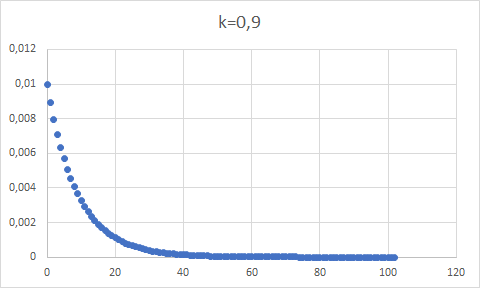
\includegraphics[width=0.4\textwidth]{../Mathematik_2/Bilder_unused/logistische_abbildung_parameter_0_9.png}
%	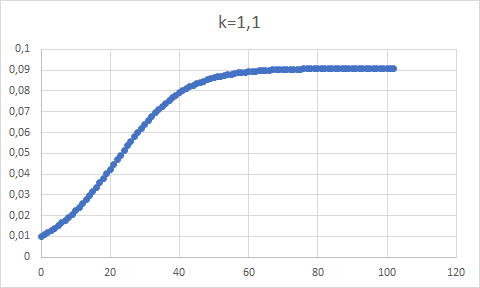
\includegraphics[width=0.4\textwidth]{../Mathematik_2/Bilder_unused/logistische_abbildung_parameter_1_1.png} \\
%	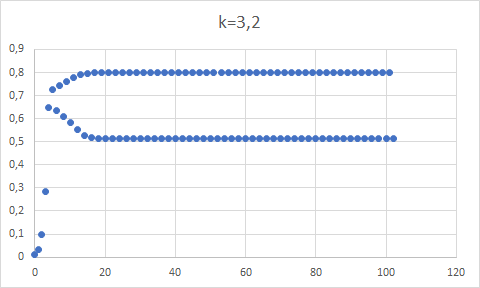
\includegraphics[width=0.4\textwidth]{../Mathematik_2/Bilder_unused/logistische_abbildung_parameter_3_2.png}
%	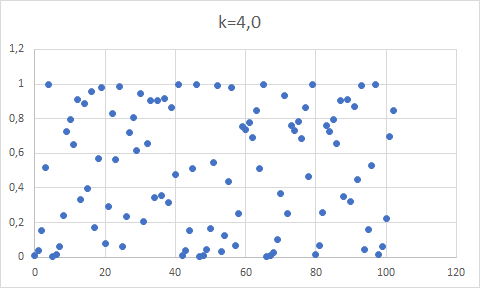
\includegraphics[width=0.4\textwidth]{../Mathematik_2/Bilder_unused/logistische_abbildung_parameter_4_0.png}
%\end{center}
%	Das System l��t Beobachtungen zu:
%	\begin{itemize}
%		\item Das Wachstum ist nach oben begrenzt durch $x=1$.
%		\item Das Wachstum ist nach unten begrenzt durch $x=0$.
%		\item Der Wachstumsprozess h�ngt von $k$ ab:
%
%			%Man kann die D�mpfung f�r $k=0.9$, die Beschr�nktheit f�r $k=1.1$ und f�r $k=3.2$ Oszillationen beobachten und f�r $k=4$ deterministisches Chaos.
%	\end{itemize}
%	%Je nachdem, welche Werte man f�r die Wachstumsrate $k$ einsetzt, verh�lt sich das System verschieden.
%	%	Beispiele  \begin{itemize}
%	%	\item $k=0,97$ \item $k=1,18$ \item $k=3,29$ \item $k=3,510$ \item $ k=3,5511$ \item $k=4,012$ \end{itemize}
%\end{exabox}
%
%	Die logistische Gleichung ist offensichtlich in der Lage drei Ph�nomene zu modellieren:
%\begin{enumerate}
%	\item Streben zu einem Gleichgewichtszustand,
%	\item Einsetzen von Schwingungen,
%	\item deterministisches Chaos.
%\end{enumerate}
%	Der Begriff deterministisches Chaos beschreibt, dass winzige Unterschiede im Anfangszustand nach wenigen Schritten deutliche Auswirkungen haben (exponentielles Fehlerwachstum). Dass die Folge der Zust�nde des Systems wie Zufall aussehen, ist nur eine Konsequenz davon. Ein weiteres Ph�nomen, das mit Hilfe der logistischen Gleichung nicht sichtbar ist, ist die Resonanzkatastrophe: das praktisch unendliche Aufschaukeln von Schwingungen.
%
%\begin{center}
%	\begin{tabular}{l|c|c}
%		Zeit / Zustandsraum
%		& diskret & kontinuierlich \\
%		\hline
%		diskret & Steuerungstechnik & digitale Regelungstechnik\\
%		\hline
%		kontinuierlich & Quantenmechanik & \textcolor{blue}{Mechanik}
%	\end{tabular}
%\end{center}
%
%Was uns im Folgenden interessiert sind dynamische Systeme, deren Zustandsraum kontinuierlich in Zeit und Raum ist. Die Entwicklungsgesetze entstammen in diesem Fall der Mechanik oder der analogen Regelungstechnik. Es sind Differentialgleichungen.

\subsection{Typen von Differentialgleichungen}

Zeitkontinuierliche dynamische Systeme werden typischerweise mit Differentialgleichungen beschrieben. Differentialgleichungen sind Gleichungen, in denen eine Ableitung oder mehrere Ableitungen einer Funktion und gegebenenfalls die Funktion selbst auftreten. Anders als beim L�sen einer Gleichung ist die L�sung einer Differentialgleichung eine Funktion und kein Wert. Das ist also eine Differentialgleichung [differential equation] und die gesuchte Gr��e ist die Funktion $f$:
		\[
			f'(x) = 3\cdot f(x) + x^2\,.
		\]
		Oft wird die Unbekannte nicht $f$ sondern $y$ genannt:
		\[
			y'(x) = 3\cdot y(x) + x^2 \,.
		\]
		In der Mechanik betrachtet man oft zeitabh�ngige Ph�nomene und die Zeitableitungen werden mit Punkten notiert, man findet also entsprechend
		\[
			\dot x(t) = 3\cdot x(t) + t^2 \,.
		\]

		\begin{defbox}{Klassifikationen von Differentialgleichungen}{ }
			\begin{itemize}
				\item Die Ordnung [order] einer Differentialgleichung gibt an, was die h�chste Ableitung ist, die in der Differentialgleichung vorkommt. Zum Beispiel ist das eine Differentialgelichung der Ordung zwei:  \[ y'' - \sin(x)\cdot y = \left( y'\right)^2\,. \]
				\item In einer expliziten [explicit] Differentialgleichung steht die h�chste Ableitung isoliert auf einer Seite und kommt ansonsten nicht vor. Zum Beispiel: \[ y'' = \sin(x)\cdot y  + \left( y'\right)^2\,. \]
				\item In einer impliziten [implicit] Differentialgleichung l��t sich die h�chste Ableitung nicht isolieren. Zum Beispiel: \[\sin(y'' + x^2) = y'\,. \]
				\item In einer linearen [linear] Differentialgleichung tritt nur eine Summe von Vielfachen der Funktion und ihrer Ableitungen auf. Diese Vielfachen d�rfen allerdings Funktionen der unabh�ngigen Variablen sein.  Zum Beispiel  \[\sin(x) \cdot y'' - 17 \cdot y' + x^2\cdot y = \cos(x) \,.\]
				\item Falls die Vielfachen einer linearen Differentialgleichung nicht Funktionen, sondern Konstanten sind, hat man eine lineare Differentialgleichung mit konstanten Koeffizienten [constant coefficients]. Die Inhomogenit�t darf dabei aber weiter eine Funktion sein. Zum Beispiel:   \[ 3\cdot y'' - 4\cdot y' + 7\cdot y = \cos(x)\,.\]
	\end{itemize}
		\end{defbox}

		\noindent Bemerkungen:

		\begin{itemize}
			\item Die Differentialgleichungen, in denen nur nach einer Unabh�ngigen abgeleitet wird, hei�en "\, gew�hnliche Differentialgleichungen"\, [ordinary differential equations]. Nur um solche geht es hier.
			\item Differentialgleichungen, in denen mehrere unabh�ngige Variablen auftauchen, hei�en partielle Differentialgleichungen. Partielle Differentialgleichungen werden hier nicht betrachtet.
			\item Die Bezeichnung "\,explizit"\, ist nicht �berall gleich definiert. Ist eine explizite Differentialgleichung eine, die nach der h�chsten Ableitung aufgel�st ist? Oder aber eine wie $\frac{ \mathrm{d} y}{\mathrm{d}x} +7=x$, die man leicht nach der h�chsten Ableitung aufl�sen kann? Einige Autoren verwenden auch den Begriff "\,explizite Form"\,, wenn die Gleichung nach der h�chsten Ableitung aufgel�st ist.
				Wir nennen eine Differentialgleichung explizit, wenn sie in expliziter Form gegeben ist.
			\item "\,Implizit"\, kann das Gegenteil von "\,explizit"\, bedeuten, wird oft aber nur f�r Gleichungen der Art $\cdots=0$ verwendet, also solchen mit Null auf einer Seite. Nach der letzteren Art der Definition ist $\frac{\mathrm{d} y}{\mathrm{d}x}=0$ implizit und explizit. � Also immer erst pr�fen, was der jeweilige Autor mit diesen Begriffen meint!
		\end{itemize}

\subsection{Existenz und Eindeutigkeit einer L�sung (+)}

Bevor man Zeit investiert, um eine L�sung einer Differentialgleichung zu bestimmen, lohnt es sich abzukl�ren, unter welchen Voraussetzung denn eine L�sung existiert und wenn eine L�sung existiert, ob sie eindeutig ist.

Die Existenzbeweise, die man in diesem Kontext f�hrt, erfordern Kenntnisse �ber die Vollst�ndigkeit normierter R�ume und �bersteigen den Rahmen dieser Vorlesung. Allerdings ist das Ergebnis f�r den Fall eines Anfangswertproblems erster Ordnung sehr griffig und leicht zu �berpr�fen und aus diesem Grund sollten wir nicht darauf verzichten.

Zuvor m�ssen wir Funktionen charakterisieren k�nnen, die eine versch�rfte Stetigkeitseigenschaft erf�llen:\marginpar{\small Aufgabe}
\begin{defbox}{Lipschitz-stetige Funktionen}{ }
	Es sei \( f:[a,b]\times \mathbb K \to \mathbb K\) eine stetige Funktion, f�r die gilt
	\[ \exists \, L\in \mathbb R:\; \forall x\in [a,b], y_1,y_2\in \mathbb K: \quad |f(x,y_1) - f(x,y_2)| \leq L|y_1-y_2| \,. \quad (*)\]
	Gilt $(*)$, so nennt man $f$ Lipschitz-stetig mit Lipschitz-Konstante $L$.
\end{defbox}

Es gilt der folgende Satz �ber Existenz und Eindeutigkeit einer L�sung eines Anfangswertprolems mit Differentialgleichung erster Ordnung.

\begin{theorembox}{Existenz und Eindeutigkeit einer L�sung}{ }
	Es sei \( f:[a,b]\times \mathbb K \to \mathbb K\) eine Lipschsitz-stetige Funktion. 	 Dann hat das Anfangswertproblem
	\[ \begin{cases} y' &= f(x,y),\\
			y(x_0) &= y_0 \,.
		\end{cases}
	\]
	mit $x_0\in [a,b]$ und $y_0\in \mathbb K$ eine eindeutige L�sung.
\end{theorembox}

\subsection{Vektorfelder und L�sungskurve}

Es gibt eine Methode, um die L�sung eines Anfangswertproblems geometrisch zu konstruieren. Bei Differentialgleichungen zweiter Ordnung l��t sich das am sch�nsten veranschaulichen. Die Idee ist die Differentialgleichung in ein System erster Ordnung umzuformen und zu verstehen, dass die rechte Seite gerade die Richtung angibt, in die sich die L�sung im Phasenraum entwickelt.

Betrachten wir beispielsweise die Differentialgleichung, die die Bewegung eines Federpendels mit Masse $m$, Federkonstante $D$, Reibungskonstante $\rho$ und Position $x$ (gemessen ab der Ruhelage) beschreibt:
		\[
			\underbrace{ m \ddot x }_{\displaystyle{ = F } }  = - D\cdot x - \rho\cdot \dot x \,.
	\]
	Der Zustandsraum (Phasenraum) sind Vektoren mit zwei Komponenten, also der Vektorraum $\mathbb R^2$ mit folgender physikalischer Zuordnung:
	\[ \left( \begin{array}{c} \textnormal{Position} \\ \textnormal{Geschwindigkeit} \end{array}\right) = \left( \begin{array}{c} x \\ \dot x \end{array}\right) \; \textnormal{ oder } \; \left( \begin{array}{c} \textnormal{Position} \\ \textnormal{Impuls} \end{array}\right) =\left(\begin{array}{c} x \\ p \end{array}\right), \textnormal{ mit } p = m\cdot \dot x\,. \]

	Wenn man beachtet, dass die Ableitung des Impulses gerade die Newtonsche Kraft ist,
	\[ \dot p = F\,, \]

	dann l�sst sich die Bewegungsgleichung so umformen, dass man sieht, wie sich der Zustandvektor \( ( x, p)^\intercal\) zeitlich entwickelt. Anstatt einer Differentialgleichung zweiter Ordnung, erhalten wir eine vektorwertige Differentialgleichung der Ordnung eins:
	\[ \begin{array}{rcl l} \dfrac{\mathrm{d}}{\mathrm{d}t} \left( \begin{array}{c} x \\p \end{array}\right) &=& \left( \begin{array}{c}  \dfrac{p}{m} \\F\end{array}\right) & \|\; F = m\cdot \ddot x \\ &=&  \left( \begin{array}{c} \dfrac{p}{m} \\ - D\cdot x - \rho \dot x \end{array}\right) &\| \; \dot x = m\cdot p  \\   &=& \left( \begin{array}{c}  \dfrac{p}{m} \\ - D\cdot x - \rho\cdot \dfrac{p}{m} \end{array}\right) &\; \textnormal{ Identifikation der Matrix-Vektor-Multiplikation} \\  &=& \left( \begin{array}{cc} 0 & \dfrac{1}{m} \\ - D   & - \dfrac{\rho}{m} \end{array}\right)\, \left( \begin{array}{c} x \\p\end{array}\right)\,. & \end{array}    \]

		Das kann man sich das Vektorfeld veranschaulichen:
		\begin{exabox}{Phasenraum Federpendel}{ }
			\begin{center}
	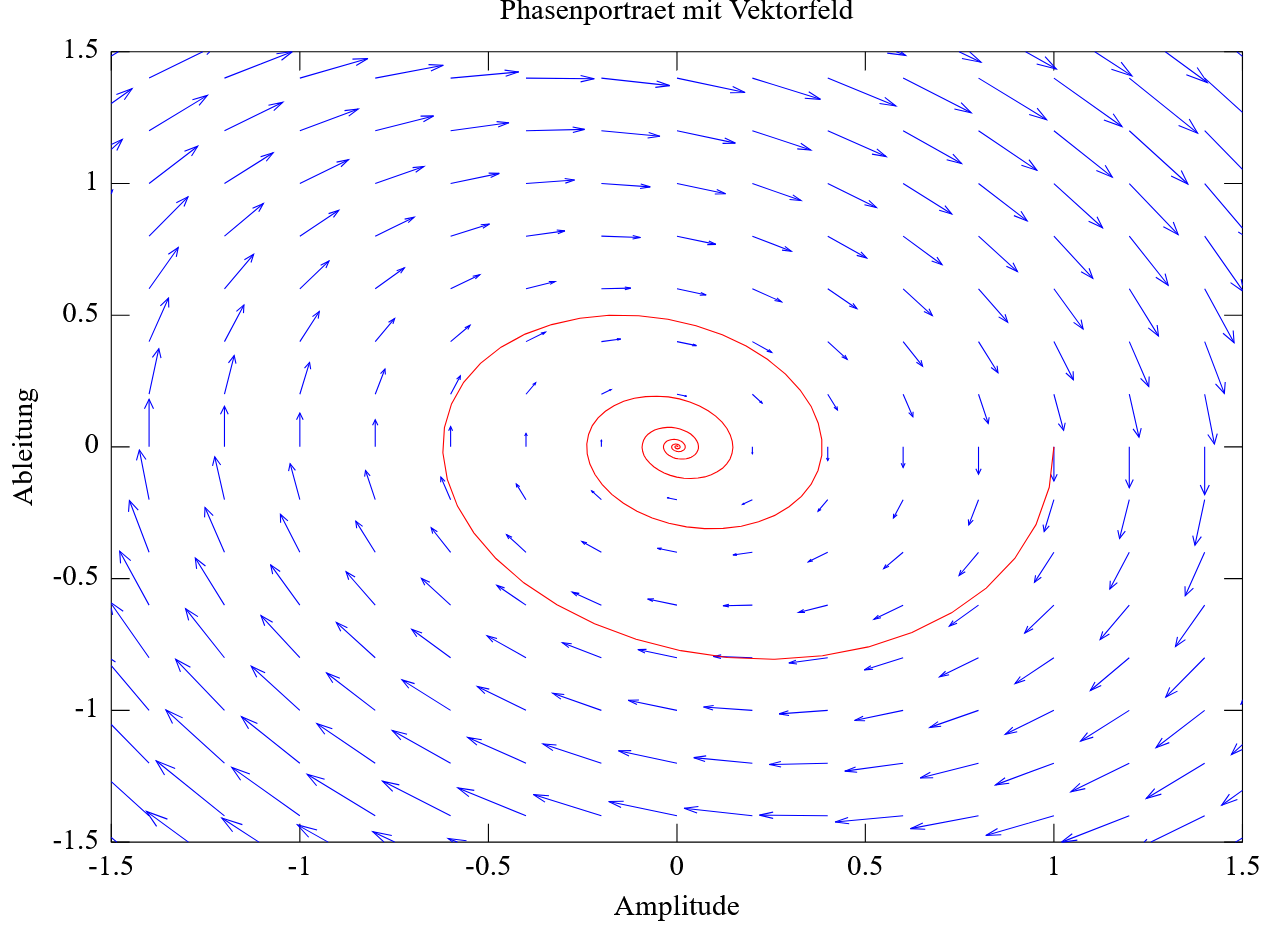
\includegraphics[width=0.8\textwidth]{../Mathematik_2/Bilder/gedaempfte_schwingung_phasenportrait_vektorfeld.png}
			\end{center}
\end{exabox}

Verbindet man im Phasenraum die nacheinander zeitlich erreichten Zust�nde, ergibt sich eine L�sungs\-kurve. Wenn man einen Punkt im Phasenraum als Anfangszustand ("\, Anfangsbedingung"\,) vorgibt, dann ist der Zustand zu jedem beliebigen Zeitpunkten danach und davor (!) eindeutig festgelegt.

Mathematisch hei�t das, dass man beweisen kann, dass es zu jeder gegebenen Anfangsbedingung $x(t_0),p(t_0)$ eine eindeutige L�sung der Differentialgleichung, also eine passende Funktion $(x(t),p(t))$) gibt. Die Existenz und Eindeutigkeit einer L�sung zu jeder Anfangsbedingung ist mathematisch nicht trivial und sie gilt auch nicht immer!

%Der Zustand kann zu endlicher Zeit ins Unendliche entweichen oder in eine Definitionsl�cke einer Funktion enden, die in der Differentialgleichung vorkommt. Theoretisch k�nnte es auch andere Probleme geben: Erstens k�nnte eine Funktion, die in der Differentialgleichung vorkommt, zu rau sein, so dass sich vielleicht gar keine L�sung finden l�sst. Zweitens k�nnte eine Funktion, die in der Differentialgleichung vorkommt, zu steil sein, so dass die L�sung verzweigen kann und damit nicht eindeutig ist.

		%Ein Beispiel f�r Letzteres ist die Differentialgleichung \[\frac{\mathrm{d}y}{ \mathrm{d}x}= v|y(x)|\,.\]
		%Zum Anfangswert $x(0)\stackrel{!}{=}0$ hat diese Differentialgleichung unendlich viele L�sungen. Eine davon ist, dass $y(x)$ dauerhaft $0$ ist. Eine andere L�sung verzweigt daraus ab $x=0$ f�r $x\geq 0$ in $y(x)=\frac14 x^2$. In der Praxis erlebt man so etwas h�chst selten. Existenz und Eindeutigkeit von L�sungen von Differentialgleichungen sind dort typischerweise anschaulich klar.

%
 \newpage % 13 Differentialgleichungen Grundlagen
%\setcounter{exercise}{0} 
\ifintegriereaufgaben
\section*{Differentialgleichungen Aufgaben}\label{MA2-differentialgleichungen-aufgaben}

Erkl�rungen und Beispiele, die zur Bearbeitung der Aufgaben hilfreich sind, finden Sie im Skript\wennreferenzvorhanden{MA2-differentialgleichungen}{ (Abschnitt \abschnittsverweis{MA2-differentialgleichungen})} und, falls Sie nicht weiterkommen, schauen Sie \hyperref[MA2-differentialgleichungen-loesungen]{hier}.

\else
\section{Differentialgleichungen Aufgaben}\label{MA2-differentialgleichungen-aufgaben}

Regeln und Beispiele zu diesen Aufgaben finden Sie im Skript. Die L�sungen finden Sie \hyperref[MA2-differentialgleichungen-loesungen]{hier}.
\fi

\begin{exercisebox}[Typeneinteilung]
	Klassifizieren Sie die folgenden Differentialgleichungen:
	\begin{itemize}
		\item[(a)] $\dot p(t) = a\cdot p(t) - b\cdot p^2(t)$
		\item[(b)] $M\ddot s(t) = As(t), \quad M, A \in \mathbb R^{2\times 2}, s:\mathbb R\mapsto \mathbb R^2\,.$
		\item[(c)] $y' = x y^2\,.$
		\item[(d)] $y\cdot y^{(4)} + x y'' + \ln(y) = 0\,.$
		\item[(e)] $\Delta u(x,y) = 0\,, \quad (x,y)\in \Omega\subset \mathbb R^2, \quad \Delta u = \displaystyle{\frac{\partial^2 u}{\partial x^2} +\frac{\partial^2 u}{\partial y^2}} $
	\end{itemize}
\end{exercisebox}

\begin{exercisebox}[Differentialgleichungen] %Papula IV, Abschnitt 1, Aufgabe 1/2
	\begin{itemize}
		\item[(a)] Zeigen Sie, dass die Funktion $y: x\mapsto c_1 \cdot e^{5x} + c_2 \cdot e^{-x}$ f�r jede Wahl von $ c_1, c_2\in\mathbb R$ die folgende Differentialgleichung l�st:
			\[ y'' - 4y' - 5y = 0 \,.\]
		\item[(b)] Zeigen Sie, dass $y: x\mapsto \displaystyle{ \frac{c\cdot x}{1+x}} $ f�r jede Wahl von $c\in\mathbb R$ die folgende Differentialgleichung l�st
			\[ x(1+x)y' - y = 0, \; x\in(-1,1) \,\]

			und bestimmen Sie $c$ so, dass auch $y(1) = 8$ gilt.
	\end{itemize}
\end{exercisebox}

\begin{exercisebox}[Asymptotik]
	Betrachten Sie das Anfangswertproblem
	\[\begin{cases}
			s(0) = 0, \quad & t_0=0\,,\\
			\dot s(t) = 1+s^2(t)\,,\quad & t > t_0\,.
	\end{cases}\]
	\begin{itemize}
		\item[(a)] Zeigen Sie, dass $s:t\mapsto \tan(t)$ eine L�sung des Anfangswertproblems ist.
		\item[(b)] Bestimmen Sie das asymptotische Verhalten der angegebenen L�sung f�r $t\to \pi/2$
		%\item[(c)] Ist die L�sung eindeutig?
	\end{itemize}
\end{exercisebox}

\begin{exercisebox}[Eindeutige L�sbarkeit]
	Betrachten Sie das Anfangswertproblem
	\[\begin{cases} y(1) = 1, \quad & x_0=1\,,\\
			(y')^2 - 4xy' + 4y = 0\,,\quad & x > x_0\,.
	\end{cases}\]
	\begin{itemize}
		\item[(a)] Klassifizieren Sie die Differentialgleichung.
		\item[(b)] Zeigen Sie, dass $y: x\mapsto 2cx-c^2$ die Differentialgleichung l�st und skizzieren Sie die Geradenschar.
		\item[(c)] Bestimmen Sie die Konstante $c$ so, dass $y$ das Anfangswertproblem l�st.
		\item[(d)] Ist die L�sung des Anfangswertproblems eindeutig?
	\end{itemize}
\end{exercisebox}

%\subsection{Praxis}
%\begin{exercisebox}[Moodle Eindeutigkeit] % HMI III; Blatt 12, Aufg. 3
%Die allgeimeine L�usng der Differentialgleichung
%\[ y'' + y = 1 \]
%lautet
%\[y(x) = c_1 \cos(x) + c_2\sin(x) + 1\,. \]
%Untersuchen Sie die Eindeutigkeit der L�sung bei Vorgabe von Anfangsbedingungen.
%\begin{itemize}
%	\item[(a)] $ y(0) = 0 \land y(\pi/2) = 1 $
%	\item[(b)] $ y(0) = 0 \land y(\pi) = 1 $
%	\item[(c)] $ y(0) = 0 \land y(\pi) = 2 $
%	\item[(d)] $ y(0) = 0 \land \left( y'(b)\right)^2 = 1, \quad 0 < b < \pi/2 $
%\end{itemize}
%\end{exercisebox}

%\subsection{Theorie}
%
%\begin{mybox}[�bersicht �ber Aufgabentypen]
%	Das Anfangswertproblem ist l�sbar, falls \(f:D_f\to \mathbb R\) bez�glich \(x\) und \(y\) stetig ist, dann besietzt das Anfangswertproblem wenigstens eine L�sungskurve in \(D_f\).
%\end{mybox}

 \newpage
\setcounter{def}{0} \setcounter{satz}{0} \setcounter{exa}{0} \section{Lineare Differentialgleichungen}\label{MA2-lineare-differentialgleichungen}

\begin{table}[H]
  \centering
  \begin{tabularx}{\textwidth}{@{}>{\raggedright\arraybackslash}X r@{}}
    \toprule
    \multicolumn{2}{c}{\textbf{�bersicht �ber Lernziele und Voraussetzungen}} \\
    \midrule
    \textbf{Lernziele} & \\[.5\normalbaselineskip]
    \tabitem homogene lineare Differentialgleichungen erster Ordnung mittels Exponentialansatz l�sen & \\
    \tabitem homogene lineare Differentialgleichungen mit konstanten Koeffizienten durch Analyse des charakteristischen Polynoms l�sen & \\
    \tabitem zugeh�rige inhomogene Differentialgleichungen l�sen & \\
    \hspace{0.7cm}\tabitem durch Variation der Konstanten (1. Ordnung) & \\
	  \hspace{0.7cm}\tabitem durch Ansatz vom Typ der rechten Seite bei konstanten Koeffizienten & \\[.5\normalbaselineskip]
    \midrule
    \textbf{Voraussetzungen} &  \\[.5\normalbaselineskip]
    \tabitem Ableitungen h�herer Ordnung berechnen k�nnen &\abschnittsverweis{MA1-ableitungsregeln}  \\
    \tabitem Exponentialfunktionen sicher handhaben k�nnen &\abschnittsverweis{MA1-exponential-und-logarithmusfunktionen} \\[.5\normalbaselineskip]
    \bottomrule
  \end{tabularx}
\end{table}

\noindent \ifintegriereaufgaben Die �bungsaufgaben zum Thema finden Sie \hyperref[MA2-lineare-differentialgleichungen-aufgaben]{hier}.
\vspace{0.3cm}
\hrule
\fi


\subsection{L�sungsstrategie}

Eine Differentialgleichung allein liefert noch kein wohldefiniertes mathematisches Problem. Neben der Gleichung, in der eine Ableitung einer gesuchten Funktion vorkommt, braucht man unbedingt noch einen Startpunkt (Anfangswert) im Phasenraum. Eine Differentialgleichung zusammen mit einer Anfangsbedingung nennt man Anfangswertproblem.
\begin{exabox}{Anfangswertproblem}{ }
Anfangswertproblem
\begin{eqnarray*}
	\begin{cases}
	y(3) = 7\,, \quad &y=3\,,  \\
	y'(x) = \sin(x)\,, \quad &y>3\,.
\end{cases}
\end{eqnarray*}
Ansatz f�r $y$:
\begin{eqnarray*}
	y(x) &=& - \cos(x) + c \,,\\
	y'(x) &=& \sin(x) \,.
\end{eqnarray*}
Bestimmung der Konstante $c$:
\[
	y(3) \stackrel{!}{=} 7 \Rightarrow c  = (7+\cos(3))\,.
\]
L�sung:
\[
	y(x) = - \cos(x) + (7+\cos(3))\,.
\]
\end{exabox}

Die L�sung eines Anfangswertproblems kann man also finden, indem man die Form der L�sung r�t (Ansatz).  Aus dem vorigen Beispiel wird deutlich, warum das L�sen von Differentialgleichungen auch Integrieren von Differentialgleichungen hei�t. Der Ansatz  - die kultivierte Art des Ratens - ist beim L�sen von Differentialgleichungen gang und g�be.

Wenn man eine L�sungsfunktion zum vorgegebenen Anfangswert angeben kann, hat man gewonnen, egal, wie man auf die L�sung gekommen ist. Denn (bis auf pathologische F�lle in der Mathematik) ist die L�sung eindeutig.

Lineare Differentialgleichungen haben, �hnlich der L�sungen inhomogener \underline{linearer Gleichungssysteme}\randverweis{MA1-lineare-gleichungssysteme}, eine wichtige Gemeinsamkeit. Ist eine Differentialgleichung linear, dann besitzt die allgemeine L�sung im Allgemeinen zwei L�sungsanteile:
\[ y(x) = y_h(x)  + y_p(x)\,, \]
wobei $y_h$ die allgemeine L�sung der homogenen Differentialgleichung und $y_p$ eine L�sung der inhomogenen Differentialgleichung ist. $y_h$ nennt man die homogene L�sung und $y_p$ nennt man eine partikul�re L�sung [particular solution] der Differentialgleichung.

Diese Superpositionseigenschaft f�hrt dazu, dass immer die folgenden L�sungsschritte anfallen:
\begin{theorembox}{L�sungsschema - Superpositionsprinzip}{ }
	\begin{enumerate}
		\item Bestimmung der allgemeinen L�sung der homogenen Differentialgleichung $y_h$.
		\item Bestimmung einer partikul�ren L�sung $y_p$ der inhomogenen Differentialgleichung.
		\item Superposition beider L�sungskomponenten $y(x) = y_p(x) + y_h(x)$.
		\item Bestimmung der Konstanten der homogenen L�sung, falls ein Anfangswert gegeben ist.
	\end{enumerate}
\end{theorembox}

Lineare Differentialgleichungen erlauben es, komplexe Dynamiken in �berlagerbare Teilprozesse zu zerlegen.
Dieser Gedanke der �berlagerung kn�pft unmittelbar an die Struktur der Funktionenr�ume an.


\subsection{Ordnung 1}

Betrachten wir lineare Differentialgleichung erster Ordnung, die so aussehen:
\[ y'(x)+f(x)\cdot y(x) = 0\,.\]

Anhand des folgenden Beispiels wird demonstriert, wie ein allgemeiner Exponentialansatz zu einer L�sung f�hrt - im Falle eines Anfangswertproblems zu einer eindeutigen L�sung:
\begin{exabox}{\(y_h(x)\) allgemeiner Exponentialansatz}{ }
	Anfangswertproblem
	\begin{eqnarray*}
		\begin{cases}
			y(1) = 7\,, &\quad x=1\,,\\
			y'(x)+\displaystyle{\frac{1}{x}}y(x) = 0\,,  &\quad x > 1\,.
		\end{cases}
	\end{eqnarray*}
	Ansatz f�r $y$:
	\begin{eqnarray*}
		y(x) &=& e^{\lambda(x)}\,,\\
		y'(x) &=& e^{\lambda(x)} \cdot \lambda'(x)\,.
	\end{eqnarray*}
Bestimmung der Funktion $\lambda:x\mapsto \lambda(x)$:
	\begin{eqnarray*}
		e^{\lambda(x)} \cdot \lambda '(x) + \frac1x e^{\lambda(x)}  \stackrel{!}{=} 0  \Leftrightarrow \lambda(x) = -\int\frac{1}{x}\,\mathrm{d}x = -\ln(|x|) + C
		\end{eqnarray*}
Bestimmung der Konstante:
\[ y(x) = c \cdot e^{-\ln(x)} = \dfrac{c}{x}, \quad c=e^{C}>0  \quad \textnormal{mit} \quad y(1) = c\cdot 1 \stackrel{!}{=} 7 \,  \Leftrightarrow  c = 7\,.
	\]
	L�sung:
			\[
				y(x) = \frac{7}{x}\,.
		\]
\end{exabox}

\noindent Bemerkungen:
\begin{itemize}
	\item Ist kein Anfangswertproblem zu l�sen, so beh�lt man die Integrationskonstante \(c\) in der L�sung bei.
\end{itemize}

Was ist zu tun, wenn die Differentialgleichung inhomogen ist? Wenn die Differentialgleichung also die folgende Struktur hat:
\[ y'(x)+f(x)\cdot y(x) = g(x)\,.\]

Entsprechend unserem L�sungsschema, bleibt nur noch die Frage zu kl�ren, wie $y_p$ zu bestimmen ist. Die L�sungsstrategie nennt sich "\, Variation der Konstante"\, und der Name ist Programm: eine partikul�re L�sung \(y_p\) besitzt dieselbe Gestalt wie die homogene L�sung, wobei f�r die Integrationskonstante eine unbekannte, von \(x\) abh�ngige Funktion anzusetzen ist. Betrachten wir ein Beispiel:

\begin{exabox}{\(y_p(x)\) Variation der Konstante}{ }
Anfangswertproblem:
	\[
		\begin{cases}
			y(\pi) = \displaystyle{\frac{1}{\pi}}\,, &\quad x=\pi\,,\\[1ex]
			y'(x) + \displaystyle{\frac{1}{x}} y(x) = \cos(x)\,,  &\quad x> \pi\,.
		\end{cases}
	\]
Homogene L�sung $y_h$:
\[ y_h(x) = c \displaystyle{\frac{1}{x}}, \quad c\in \mathbb R \,.
\]
Ansatz f�r $y_p$:
\begin{eqnarray*}
	y_p(x) &=& c(x)\displaystyle{\frac{1}{x}}\,,\\
	y'_p(x) &=& c'(x)\displaystyle{\frac{1}{x}} - c(x)\displaystyle{ \frac{1}{x^2}}\,.
\end{eqnarray*}
Bestimmung der Funktion $c:x\mapsto c(x)$:
		\begin{eqnarray*}
			\begin{array}{l rcl}
				&\quad c'(x)\displaystyle{\frac{1}{x}} - c(x) \displaystyle{ \frac{1}{x^2}} + c(x) \displaystyle{\frac{1}{x^2}} &\stackrel{!}{=}& \cos(x) \\[2ex]
				\Leftrightarrow & \quad c'(x) &=& x\cdot \cos(x) \\
				\Leftrightarrow &\quad c(x) & = & \displaystyle{\int} x\cdot \cos(x) \,\mathrm{d}x = \cos(x) + x\sin(x)\,.
		\end{array}
	\end{eqnarray*}
	Partikul�re L�sung:
	\[
y_p(x) = \frac{\cos(x) + x\sin(x) }{x}
\]
Superposition der L�sungskomponenten:
		\[ y(x) = y_p(x) + y_h(x) = c\frac{1}{x} + \frac{\cos(x) + x\sin(x) }{x}\,.\]
Bestimmung der Konstante:
	\[ y(\pi) = \frac{c-1}{\pi} \stackrel{!}{=} \frac{1}{\pi} \Rightarrow c=2\,.\]
L�sung:
	\[ y(x) =  \frac{2}{x} + \frac{\cos(x) + x\sin(x) }{x}\,.\]
\end{exabox}

\subsection{Ordnung 1 mit konstanten Koeffizienten}

Betrachten wir nun eine Differentialgleichungen erster Ordnung, die so aussieht:
\[ y'(x) + a y(x) = 0,\quad a \in \mathbb R\,.\]

\begin{exabox}{\(y_h(x)\) Exponentialansatz}{ }
Anfangswertproblem
	\begin{eqnarray*}
		\begin{cases}
			y(1)  = 7\,,\quad  &x=1\,, \\
			y'(x)+5y(x) = 0\,,\quad &x>1\,.
		\end{cases}
	\end{eqnarray*}
	Ansatz f�r $y$:
	\begin{eqnarray*}
		y(x) &=&  c\cdot e^{\lambda x}, \quad c\not 0 \,,\\
		y'(x) &=&  \lambda\cdot c\cdot e^{\lambda x}\,.
	\end{eqnarray*}
Bestimmung der L�sung $y:x\mapsto y(x)$:
	\begin{eqnarray*}
		y'(x) + 5 y(x) = \lambda\cdot c\cdot e^{\lambda x} + 5 \cdot c\cdot e^{\lambda x}  \stackrel{!}{=} 0 \stackrel{(*)}{\Leftrightarrow}  \lambda + 5\stackrel{!}{=} 0  \Rightarrow \lambda = -5\,,
		\end{eqnarray*}
		wobei \( (*)\), da  \(\quad  c\not=0 \land \forall x\in \mathbb R e^{\lambda x}\not=0\,.\)

		\vspace{0.2pt}
Bestimmung der Konstante $c$:
		\[
			y(x)= c \cdot e^{-5 x }\quad\textnormal{mit} \; y(1)  \stackrel{!}{=} 7 \Rightarrow  c \cdot e^{-5} \stackrel{!}{=} 7 \Rightarrow c = 7 e^{5} \,.
\]
L�sung:
			\[ y(x) = 7 \cdot e^{5} e^{-5 x} \,.\]
\end{exabox}

Offensichtlich liefert der Ansatz \(y(x) = c e^{\lambda x}\) eine L�sungsstrategie f�r eine homogene Differentialgleichung mit konstantem Koeffizient.
\noindent Bemerkungen:
\begin{itemize}
	\item Die L�sungsstrategie verschleiert, dass die Konstante \(c\) eine Integrationskonstante ist. Um das zu verstehen, l�sen Sie die Differentialgleichung nach dem Schema "\, \underline{Trennbare Variablen}"\randverweis{MA1-polynome}.
	\item Ist man an einer allgemeinen L�sung der homogenen Differentialgleichung interessiert, dann beh�lt man die Integrationskonstante \(c\) in der L�sung bei.
\end{itemize}

Was, wenn die Differentialgleichung inhomogen ist? Wenn die Differentialgleichung also die folgende Struktur hat:
\[ y'(x)+ a\cdot y(x) = g(x)\,.\]
Die allgemeine L�sung der inhomogenen Differentialgleichung setzt sich wieder aus homogener und partikul�rer L�sung zusammen und die Frage ist, wie \(y_p\) zu bestimmen ist. Die Strategie nennt sich "\,Ansatz vom Typ der rechten Seite". Betrachten wir ein Beispiel.

\begin{exabox}{\(y_p(x)\) Ansatz vom Typ der rechten Seite}{ }
Differentialgleichung:
\[
y'(x) + 5y(x) = x^2\,.
\]
Homogene L�sung:
\[
	y_h(x) = ce^{-5x} \,.
\]
Ansatz f�r $y_p$:
\begin{eqnarray*}
	y_p(x) &=& A_1x^2 + A_2x + A_3\,,\\
	y_p'(x) &=& 2A_1x + A_2\,.
\end{eqnarray*}
Bestimmung der Koeffizienten f�r $y_p$
		\begin{eqnarray*}
			&&2A_1x + A_2 + 5 A_1 x^2 + 5A_2x + 5A_3 \stackrel{!}{=} x^2 \; \Leftrightarrow \; \begin{cases}  5A_1 &= 1 \\
				2A_1 + 5 A_2 &= 0 \\
			A_2 + 5A_3 &= 0 \end{cases} \; \Leftrightarrow \;
			\begin{cases} A_1 &= 1/5 \\ A_2 &= - 2/25 \\
			A_3 &= 2/125 \end{cases}
		\end{eqnarray*}
Partikul�re L�sung:
\[
			y_p(x) = \frac15 x^2 - \frac{2}{25} x + \frac{2}{125}\,.
\]
Superposition beider L�sungsanteile:
		\[ y(x) = y_p(x) + y_h(x) = \frac15 x^2 - \frac{2}{25} x + \frac{2}{125} + ce^{-5x}\,.\]
\end{exabox}

\begin{theorembox}{Ans�tze vom Typ der rechten Seite}{}
	Betrachten wir eine Differentialgleichung erster Ordnung
\[ y'+ay=f(x), \quad a\in \mathbb R \]
mit Inhomogenit�t \[f:I\to \mathbb R, x\mapsto p(x) \cdot e^{\mu x}\cdot  \cos(\beta x) + q(x)\cdot e^{\mu x}\cdot  \sin(\beta x)\,,\]
wbei $\mu,\beta \in \mathbb R$ und $p$ ein Polynom vom Grad \(m\) und $q$ ein Polynom vom Grad $n$.


Dann lautet der Ansatz f�r \(y_p\)
\[ y_p(x) = P(x)\cdot e^{\mu x}\cdot \cos(\beta x) + Q(x)\cdot e^{\mu x}\cdot \sin(\beta x)\,,
\]
wobei \(P\) ein Polynom vom Grad \(m\) und \(Q\) ein Polynom vom Grad \(n\) ist:
\begin{eqnarray*}
	P(x) &=& A_m x^m + A_{m-1} A^{m-1} + \cdots + A_0\,, \\
	Q(x) &=& B_n x^n + B_{n-1} x^{n-1} + \cdots + B_0\,.
\end{eqnarray*}
\end{theorembox}

\begin{exabox}{Ans�tze vom Typ der rechten Seite}{ }
	\[
		\begin{array}{rcl c rcl }
			f(x) &=& \cos(3x)  &\Rightarrow&  y_p &=& A \cos(3x) + B \sin(3x)\,,\\
			f(x) &=& e^{4x}  &\Rightarrow&  y_p &=& A e^{4x}\,,\\
			f(x) &=& \cos(3x) \cdot e^{4x}  &\Rightarrow&  y_p &=& \left(A\cos(3x) + B\sin(3x)\right) e^{4x}\,,\\
			f(x) &=& \cos(3x) + e^{4x}  &\Rightarrow&  y_p &=& A\cos(3x) + B\sin(3x) + C e^{4x}\,,\\
			f(x) &=& x^2  &\Rightarrow&  y_p &=& A_2x^2 + A_1 x + A_0\,.
		\end{array}
	\]
\end{exabox}


\subsection{Ordnung \(n\) mit konstanten Koeffizienten}

Homogene, lineare Differentialgleichungen zweiter Ordnung mit konstanten Koeffizienten sind Ihnen wahrscheinlich schon begegnet:
\begin{itemize}
	\item In der Mechanik lautet die Bewegungsgleichung f�r einen ged�mpften harmonischen Oszillator
\[
	m\ddot x = - Dx - \rho \dot x \,,
\]
wobei $\boldsymbol x$ die Auslenkung beispielsweise eines Pendels, $m$ seine Masse, $D$ die Federkonstante und $\rho$ die Reibungskonstante ist.
\item In der Elektrodynamik wird der elektrische Schwingkreis durch die folgende Differentialgleichung beschrieben
\[
	\ddot i = - \frac{1}{LC} i \,,
\]
wobei \(i\) die Stromst�rke, $C$ die Kapazi�t des Kondensators und $L$ die Induktivit�t der Spule ist.
\end{itemize}

\noindent Bemerkungen:
\begin{itemize}
	\item Es lohnt sich jetzt kurz zu �berlegen, was f�r eine L�sungskurve wir beim ged�mpften harmonischen Oszillator erwarten! Haben Sie eine Idee? \randverweis{MA1-komplexe-zahlen-polarform-und-euler}
	\item Die unahbh�ngige Variable, in den zuletzt genannten Differentialgleichungen, ist die Zeit $t$.
	\item Die Differentialgleichungen sind so keinesfalls eindeutig l�sbar - es m�ssen noch zwei Anfangsbedingungen gegeben sein.
\end{itemize}

Die L�sungstrategie entspricht dem Vorgehen aus dem vorangegangenen Abschnitt. Schauen wir uns ein konkretes Beispiel an.

\begin{exabox}{\(y_h(x)\) Exponentialansatz}{ }
	Anfangswertproblem:
\[
	\begin{cases}
		x(0)  = 1, \quad &t=0\,,\\[1ex]
		\dot x(0)  = -1, \quad &t=0\,,\\[1ex]
		\ddot x(t) = - 2\dot x(t) - 5\cdot  x(t)\,, \quad &t >0  \,.
	\end{cases}
\]
Ansatz f�r $x$:
\begin{eqnarray*}
	x(t) &=& c\cdot e^{\lambda t}, \; c>0, \quad \lambda \in \mathbb C\,. \\
				\dot x(t) &=& c \cdot \lambda  \cdot e^{\lambda t}\,,\\
				\ddot x(t) &=& c \cdot \lambda^2 \cdot e^{\lambda t}\,
			\end{eqnarray*}
Bestimmung von $\lambda$:
			\begin{eqnarray*}
				\begin{array}{r rcl}
					& \lambda^2\cdot c\cdot e^{\lambda t} + 2\cdot c\cdot \lambda e^{\lambda t} + 5\cdot c\cdot e^{\lambda t} &=& 0\, \\[1ex]
					\Leftrightarrow & \left( \lambda^2   + 2 \lambda + 5 \right)\cdot  c \cdot e^{\lambda t} &=& 0, \; c\cdot e^{\lambda t} \not=0\,,\\[1ex]
				{\Leftrightarrow}& \, \lambda^2 + 2\cdot \lambda + 5 &=& 0 \quad \Rightarrow \lambda _{1,2}= - 1 \pm 2i
		\end{array}
		\end{eqnarray*}
Allgemeine L�sung:
		\[
			\forall \; c_1, c_2 \in \mathbb C: \quad  x(t) = c_1\cdot  e^{\lambda_1\, t} + c_2 \cdot e^{\lambda_2\, t} =  e^{-t}\cdot \left( c_1\cdot   e^{2i\,t} + c_2\cdot e^{-2i\, t}\right) \,.
	\]
Bestimmung der Konstanten $c_1$ und $c_2$:
\begin{eqnarray*}
			&&\begin{cases} c_1  + c_2  &= 1\,,\\
				c_1 \cdot (-1+2i)  + c_2\cdot (-1-2i)   &= -1
			\end{cases} \\[1ex]
			\Leftrightarrow  && \left( \begin{array}{cc} 1 &  1  \\ -1+2\,i &  -1-2\,i\end{array}\right) \left( \begin{array}{c} c_1  \\ c_2\end{array}\right) = \left( \begin{array}{c} 1  \\ -1\end{array}\right) \; \Rightarrow c_1 = c_2 = \frac12\,.
		\end{eqnarray*}
		L�sung:
		\[
			x(t) = \frac12 e^{-t} \cdot \left( e^{2i\,t} + e^{-2i\, t}\right) = e^{-t}\cdot \cos(2\,t) \,.
	\]
\begin{center}
	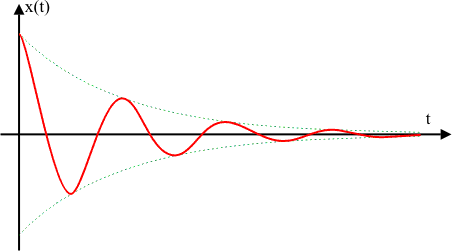
\includegraphics[width=0.7\textwidth]{../Mathematik_2/Bilder/federpendel_gedaempfte_schwingung_zeitverlauf.png}
\end{center}
\end{exabox}

\noindent Bemerkungen:
\begin{itemize}
	\item Das Polynom, dessen Nullstellen die Werte f�r $\lambda$ liefert nennt man das charakteristische Polynom $p$.  Im Beispiel ist $p:\lambda \mapsto  \lambda^2   + 2\cdot \lambda + 5$.
	\item Man erh�lt typischerweise zwei verschiedene L�sungen $\lambda_{1,2}$ und �ber die L�sungsanteile l��t sich folgendes sagen:
		\begin{itemize}
			\item $\mathrm{Im}(\lambda_{1,2})\not= 0 \Rightarrow$ Sinusf�rmige Schwingung enthalten.
			\item $\mathrm{Re}(\lambda_{1,2}) < 0 \Rightarrow $ Die L�sung klingt exponentiell ab.
			\item $\mathrm{Re}(\lambda_{1,2}) > 0 \Rightarrow $ Die L�usng w�chst exponentiell.
		\end{itemize}
	\item Die L�sungsfunktion zu $\lambda_1$ und diejenige zu $\lambda_2$ k�nnen beliebig superponiert werden, weil die Differentialgleichung linear und homogen ist. Dies liefert zwei Integrationskonstanten und so die M�glichkeit, alle erdenklichen Anfangswerte einzustellen, falls die beiden $\lambda_1\not=\lambda_2$ verschieden voneinander sind.
	\item Wenn $\lambda_1 = \lambda_2 = \lambda$ eine doppelte Nullstelle des charakteristischen Polynoms ist, dann muss man eine weitere linear unabh�ngige L�sung der homogenen Gleichung hinzuf�gen. Eine zweite linear unabh�ngige L�sung der Differentialgleichung lautet $t \cdot e^{\lambda t}$. Die die allgemeine L�sung ist dann:
		\[
			x(t) = c_1\cdot e^{\lambda \,t} + c_2\cdot t\cdot e^{\lambda \,t}\,.
		\]
	\item Eine Basis des L�sungsraums der homogenen Gleichung nennt man auch Fundamentalsystem (siehe Beispiel \ref{bsp_fs}).
	\item Falls man zwei unterschiedliche homogene L�sungen $\phi_1, \phi_2$ gegeben hat und man m�chte �berpr�fen, ob sie den L�sungsraum aufspannen, also linear unahbh�ngig sind, dann gibt es ein notwendig und hinreichendes Kriterium: man berechnet die sogenannte Wronski-\underline{Determinante}\randverweis{MA1-determinante-und-inverse}.
		\[ W(x) = \mathrm{det} \left( \begin{array}{cc} \phi_1(x) & \phi_2(x) \\ \phi'_1(x) & \phi'_2(x) \end{array}\right) \]
		Gilt $W(x) \not = 0$, so ist \( (\phi_1, \phi_2)\) ein Fundamentalsystem.
	\item Zur Bestimmung der Integrationskonstanten ist ein \underline{lineares Gleichungssystem}\randverweis{MA1-lineare-gleichungssysteme} zu l�sen.
\end{itemize}

\begin{exabox}{Fundamentalsystem}{ }\label{bsp_fs}
	Differentialgleichung:
	\[ y''+4y' + 4y = 0\,.\]
	Ansatz f�r $y$:
	\begin{eqnarray*}
		y(x) &=& e^{\lambda x}\,,\\
		y'(x) &=& \lambda e^{\lambda x}\,,\\
		y''(x) &=& \lambda^2 e^{\lambda x}\,.
	\end{eqnarray*}
	Bestimmung von $\lambda$:
	\begin{eqnarray*}
		\begin{array}{l rcl}
			&\lambda^2 e^{\lambda x} +4\lambda e^{\lambda x} +4 e^{\lambda x} &\stackrel{!}{=}& 0 \\[1ex]
			\Leftrightarrow &(\lambda^2 +4\lambda  +4)\cdot e^{\lambda x} &=& 0 \\
			\Leftrightarrow  &\lambda^2 +4\lambda+4 &=& 0  \quad \Rightarrow \lambda_{1,2} = -2 \,.
	\end{array}
	\end{eqnarray*}
	Fundamentalsystem:
	\[
	(e^{-2x}, xe^{-2x})\,, \quad \textnormal{ da } W(x) = \mathrm{det}\left( \begin{array}{cc} e^{-2x} &  x e^{-2x} \\-2 e^{-2x} & (1-2x)e^{-2x} \end{array}\right) = e^{-4x} \not=0\,.
\]
\end{exabox}

Ist die L�sung komplex, das hei�t es gibt auch echt imagin�re Anteile, dann gibt man im Allgemeinen die physikalisch sinnvolle L�sung an und das ist der Realteil der komplexen L�sung. Es liegt aus diesem Grund nahe den Ansatz f�r \(y_h\) schon auf den reellen Anteil zu reduzieren und das gelingt wie folgt: wenn \(\lambda = a+ib\) mit \(b\not= 0\) eine Nullstelle des charateristischen Polynoms ist, dann ist auch \(\overline \lambda = a-ib\) Nullstelle des charakteristischen Polynoms. Der herk�mmliche Ansatz f�r dieses P�rchen von Nullstellen lautet
\begin{eqnarray*} y_h(x) = c_1 e^{(a+ib)x} + c_2 e^{(a-ib)x} = e^{ax}\left( c_1 e^{ibx} + c_2 e^{-ibx}\right)\quad \textnormal{mit}\quad c_1 = x_1 + i y_1, c_2 = x_2 + i y_2 \in \mathbb C\,.\end{eqnarray*}
Formen wir den Ansatz mit Hilfe der \underline{Eulerschen Identit�t}\randverweis{MA1-komplexe-zahlen-polarform-und-euler} um!
\begin{eqnarray*} y_h(x) &=& e^{ax}\left( c_1 e^{ibx} + c_2 e^{-ibx}\right) = e^{ax}\left(  c_1 \left( \cos(bx) + i \sin(bx)\right) + c_2 \left( \cos(bx) - i \sin(bx) \right) \right)\,. \end{eqnarray*}
Um nun einen vern�nftigen Ansatz allein f�r eine relle L�sung abzuleiten, muss man offensichtlich die Multiplikation mit den komplex-wertigen Konstanten durchf�hren:
\begin{eqnarray*} y_h(x)
	&=&  e^{ax}\left(  (x_1 + i y_1) \left( \cos(bx) + i \sin(bx)\right) + (x_2 + i y_2) \left( \cos(bx) - i \sin(bx) \right) \right)  \\
	&=&  e^{ax} \left( (x_1 + x_2) \cos(bx) + ( y_2 - y_1) \sin(bx) \right) + i e^{ax} \left( (y_1 + y_2) \cos(bx) + ( x_1 - x_2) \sin(bx) \right) \\[1ex]
	\Rightarrow&& \mathrm{Re}\left(y_h\right)(x) = e^{ax} \left( (x_1 + x_2) \cos(bx) + ( y_2 - y_1) \sin(bx) \right) \,.
\end{eqnarray*}

Es lohnt sich dieses Ergebnis zusammen zu fassen:
\begin{theorembox}{Ansatz f�r Realteil der L�sung f�r ein komplexes Nullstellen-P�rchen}{ }
	Gilt \(p(\lambda) = p(\overline \lambda) = 0\) f�r eine komplexe Zahl \(\lambda = a+ib\) mit \(b\not=0\), so gilt:
	\[ \mathrm{Re}\left(y_h\right)(x) = e^{ax} \left( c_1 \cos(bx) + c_2 \sin(bx) \right) \quad \textnormal{mit}\quad c_1, c_2 \in \mathbb R\,. \]
\end{theorembox}


Die Differentialgleichung des Federpendels gibt es auch in einer inhomogenen Variante: Man regt das Pendel mit einer oszillierenden Kraft mit Kreisfrequenz $\omega$ und der Amplitude $\hat F$ an:
\[
	m\ddot x +\rho \dot x + D x =\hat F \cos(\omega t)\,.
\]

Hier geht man so vor, wie wir es schon bei der Differentialgleichung erster Ordnung gesehen haben: zu der allgemeinen L�sung der homogenen Differentialgleichung $x_h$ wird eine partikul�re L�sung $x_p$ der inhomogenen Differentialgleichung hinzuaddiert und erh�lt die allgemeine L�sung der inhomogenen Differentialgleichung:
\[
	x(t) = x_h(t) + x_p(t) \,.
\]
Eine Strategie zur Bestimmung einer partikul�ren L�sung ist ein Ansatz vom Typ der rechten Seite.\footnote{Bei Polynomen muss der Polynomgrad entsprechend der Ordnung der Differentialgleichung erh�ht werden!}

\begin{exabox}{\(y_p(x)\) Ansatz vom Typ der rechten Seite}{ }
	Anfangswertproblem:
\[
	\begin{cases}
		x(t_0)  = y_0, \quad &t=t_0\,,\\[1ex]
		\dot x(t_0)  = y_1, \quad &t=t_0\,,\\[1ex]
		m\ddot x(t) +\rho \dot x(t) + D x(t) =\hat F \cos(\omega \cdot t)\,, \quad &t>t_0  \,.
	\end{cases}
\]
Homogene L�sung \(x_h\):
\[ x_h(t) = c_1 e^{\lambda_1 t} + c_2e^{\lambda_2 t}  \textnormal{ mit } \lambda_{1,2}= \frac{-\rho + \sqrt{\rho^2 \pm 4m D}}{2m}, \; \lambda_1 \not= \lambda_2\,.
	\]
Ansatz f�r $x_p$:
\begin{eqnarray*}
	x_p(t) &=&  a\cos(\omega \cdot t) + b \sin(\omega \cdot t)\,,\\[1ex]
	\dot x_p(t) &=&  -\omega a\sin(\omega \cdot t) + \omega b \cos(\omega \cdot t)\,,\\[1ex]
	\ddot x_p(t) &=&  -\omega^2 a\cos(\omega \cdot t) - \omega^2 b \sin(\omega \cdot t)\,.
	\end{eqnarray*}
Bestimmung der Koeffizienten $a$ und $b$:
\begin{eqnarray*}
	\forall \, t> t_0:\quad m\ddot x_p +\rho \dot x_p + D x_p =\hat F \cos(\omega \cdot t) & \Leftrightarrow & \begin{cases} \left( - m\omega^2 + D\right)\cdot  a + \rho \omega b &\stackrel{!}{=} \hat F\,,\\[1ex]
		\left( - m\omega^2 + D\right)\cdot  b - \rho \omega a &\stackrel{!}{=} 0\,.
	\end{cases} \\
	&\Leftrightarrow & \begin{cases}
		a &= \displaystyle{ \frac{ D-m\omega^2}{(D-m \omega^2)^2 + (\omega \rho)^2}}\hat F\,,\\
		b &= \displaystyle{ \frac{\omega \rho}{(D-m\omega^2)^2 + (\omega \rho)^2}}\hat F\,.
	\end{cases}
\end{eqnarray*}
	Superposition der L�sungskomponenten:\footnote{
		Ist ein Anfangswertproblem zu l�sen, m�ssen noch die Integrationskonstanten $c_1$ und $c_2$ bestimmt werden.}
		\begin{eqnarray*}
		x(t) &=& x_p(t) + x_h(t) \\
		&=&  \displaystyle{ \frac{ D-m\omega^2}{(D-m \omega^2)^2 + (\omega \rho)^2}}\hat F \cos(\omega \cdot t) + \displaystyle{ \frac{\omega \rho}{(D-m\omega^2)^2 + (\omega \rho)^2}}\hat F \sin(\omega \cdot t) + c_1 e^{\lambda_1 t} + c_2 e^{\lambda_2 t} \,,\\[1ex]
	\end{eqnarray*}
\end{exabox}

\subsection*{Sonderfall: mathematische Resonanz}

Beim Ansatz f�r eine partikul�re L�sung kann es vorkommen,
dass der gew�hlte Ansatz bereits eine L�sung der homogenen Gleichung ist.

Beispiel:
\[
y''+y=\sin(x)
\]

Die homogene Gleichung besitzt die L�sung
\[
y_h(x)=c_1\cos(x)+c_2\sin(x).
\]

Der �bliche Ansatz
\[
y_p(x)=a\sin(x)+b\cos(x)
\]
liegt also bereits im L�sungsraum der homogenen Gleichung und liefert daher keine neue L�sung.

Man spricht in diesem Fall vom \textbf{mathematischen Resonanzfall}.

\medskip

\textbf{Regel:}

Liegt mathematische Resonanz vor, wird der Ansatz mit \(x\) multipliziert.

\[
y_p(x)=x\left(a\sin(x)+b\cos(x)\right)
\]

Allgemein gilt:

Ist der Ansatz bereits L�sung der homogenen Gleichung,
so wird er mit einer hinreichenden Potenz von \(x\) multipliziert,
bis eine linear unabh�ngige Funktion entsteht.

\medskip
Der Begriff Resonanz ist nicht zuf�llig gew�hlt:
Auch in physikalischen Systemen tritt Resonanz auf,
wenn eine �u�ere Anregung dieselbe Frequenz besitzt
wie eine Eigenfrequenz des Systems.
%
%\subsection{Mathematische Resonanz (+)}
%
%Eine Situation ist bis jetzt noch nicht aufgetregen. Betrachten wir beispielsweise die Differentialgleichung \[ y'' + y = \sin(x)\,.\] Unser herk�mmlicher Ansatz f�r die partikul�re L�sung ist
%\begin{eqnarray*}
%	y_p(x) &=& a \sin(x) + b\cos(x)\,,\\
%	%y_p'(x) &=& a\cos(x) - b\sin(x)\,,\\
%y_p''(x) &=& -a\sin(x) - b\sin(x)\,.
%\end{eqnarray*}
%Um die Konstanten \(a\) und \(b\) zu bestimmen, setzen wir den Ansatz in die Differentialgleichung ein und erhalten \ldots nichts\marginpar{!!!} - sehen Sie selbst: \[ -a\sin(x) - b\sin(x) + a\sin(x) + b\cos(x) = 0 \textnormal{ !} \] Offensichtlich l�st \(y_p\) die homogenen Gleichung! In der Tat, denn die Nullstellen des charakteristischen Polynoms sind \(\lambda_{1,2} = \pm i\) und damit lautet die allgemeine, reelle L�sung der homogenen Gleichung
%\[ \mathrm{Re}\left(y_h\right)(x) = c_1 \cos(x) + c_2\sin(x) = y_p(x)\,.\]
%H�tten wir uns zuerst Gedanken �ber \(y_h\) gemacht, h�tten wir wahrscheinlich schon l�ngst festgestellt, dass die Inhomogenit�t auf der rechten Seite selbst L�sung der homogenen Gleichung ist! Diesen Fall bezeichnet man als den mathematischen Resonanzfall.
%
%Liegt der Resonanzfall vor, muss der Ansatz f�r die partikul�re L�sung modifiziert werden: \[ y_p(x) = x\left( a \sin(x) + b\cos(x) \right)\,.\]
%
%\begin{exabox}{Mathematischer Resonanzfall}{ }
%	Differentialgleichung: \[ y'' + y = \sin(x)\]
%	Allgemeine, reelle L�sung der homogenen Gleichung:
%	\[  \mathrm{Re}\left(y_h\right) = c_1 \cos(x) + c_2 \sin(x)\quad \Rightarrow \textnormal{ mathematischer Resonanzfall} \]
%	Ansatz f�r partikul�re L�sung:
%	\begin{eqnarray*} y_p(x) &=& x\left( a \sin(x) + b\cos(x) \right)\\
%	%y_p'(x) &=& a\sin(x) +b\cos(x) + x\left(a\cos(x) - b\sin(x)\right)\\
%y_p''(x) &=& 2a\cos(x) - 2b\sin(x)  + x\left( -a\sin(x) -b\cos(x) \right) \,. \end{eqnarray*}
%	Bestimmung der Konstanten \(a, b\):
%	\begin{eqnarray*}
%		&& 2 a\cos(x) - 2b\sin(x) + x\left( -a\sin(x) -b\cos(x) \right) + x\left( a \sin(x) + b\cos(x) \right) = 2a \cos(x) - 2 b \sin(x) \\
%		\Rightarrow && 2a \cos(x) - 2 b \sin(x) \stackrel{!}{=} \sin(x)  \Rightarrow a=0\land b=-\frac12\,.
%	\end{eqnarray*}
%	Allgemeine L�sung der Differentialgleichung: \[ y(x) = y_h(x) + y_p(x) = c_1 \cos(x) + c_2 \sin(x) -\frac12 x\cos(x)\,. \]
%\end{exabox}
%
%\begin{exabox}{Ansatz f�r \(y_p\) im Fall mathematischer Resonanz}{ }
%	Differentialgleichung:
%	\[ y^{(4)} + 3 y''' + 6 y'' + 4 y' + 5y = -8 \cos(x) - 8 \sin(x)\,. \]
%	Charakteristisches Polynom: \[ p(\lambda) = (\lambda^2+1)\cdot (\lambda^2+ 4 \lambda^2 + 5) \quad  \Rightarrow p(\lambda) = 0 \Leftrightarrow \lambda \in \{ \pm i, -2 \pm i\} \]
%	Allgemeine, reelle L�sung der homogenen Gleichung: \[ \mathrm{Re}\left(y_h\right)(x) = c_1 \cos(x) + c_2 \sin(x) + e^{-2x} \left( c_3 \cos(x) + c_4 \sin(x)\right)  \quad \Rightarrow \textnormal{ mathematischer Resonanzfall} \]
%	Ansatz f�r partikul�re L�sung: \[ y_p(x) = x (a \sin(x) + b\cos(x) ) \,.\]
%\end{exabox}
%
%
%\begin{exabox}{Ansatz f�r \(y_p\) im Fall mathematischer Resonanz}{ }
%	Differentialgleichung:
%\[ y'' + y = x\sin(x) \]
%Charakteristische Polynom: \[p(\lambda) = \lambda^2 + 1 \quad \Rightarrow  p(\lambda) = 0 \Leftrightarrow  \lambda \in \{  \pm i \}\]
%Allgemeine, reelle L�sung der homogenen Gleichung: \[ \mathrm{Re}\left(y_h\right)(x) = c_1 \cos(x) + c_2 \sin(x) \quad \Rightarrow \textnormal{ mathematischer Resonanzfall}\]
%Ansatz f�r partikul�re L�sung: \[ y_p(x) = x(a_1x + a_0) \sin(x) + x(b_1x +b_0) \cos(x) \,.\]
%\end{exabox}
%
%
%Eine lineare Differentialgleichung der Ordnung \(n\geq 1\) mit konstanten Koeffizienten
%\[ y^{(n)}(x) + a_{n-1} y^{(n-1)}(x) + \cdots + a_1y^{(1)}(x) + a_0 y(x) = g(x)\,.\]
%
%Die L�sungsstrategie ist wie folgt:
%\begin{itemize}
%	\item Die L�sungsstrategie zur L�sung einer inhomogenen, linearen Differentialgleichung mit konstanten Koeffizienten der Ordnung $n$-ter Ordnung ist entsprechend:
%		\begin{enumerate}
%			\item Bestimmung der allgemeinen L�sung der homogenen Gleichung mit Hilfe des Ansatzes \(y_h(x) = e^{\lambda \cdot x}\).
%			\item Vervollst�ndigung des L�sungsraums zu \(n\) linear unabh�ngigen L�sungsfunktionen, falls das charakteristische Polynom mehrfache Nullstellen besitzt.
%			\item Falls \(g\not = 0\), erfolgt die Bestimmung einer partikul�ren L�sung \(y_p\) mit einem Ansatz vom Typ der rechten Seite, hierbei auf mathematische Resonanz achten.
%			\item Superposition beider L�sungskomponenten.
%			\item Falls ein Anfangswertproblem zu l�sen ist, erfolgt die Bestimmung der \(n\) Konstanten durch die \(n\) Anfangsbedingungen.
%		\end{enumerate}
%	\item Eine eindeutige L�sung ist nur m�glich wenn $n$ Anfangsbedingungen vorgegeben sein, beispielsweise:
%\[ y(x_0), \, y'(x_0), \cdots  y^{(n-1)}(x_0) \] Pro Integrationsschritt kommt ja eine Konstante hinzu! Die L�sung einer Differentialgleichung $n$-ter Ordung ohne fixierten Anfangsbedingungen nennt man die allgemeine L�sung [general solution].
%\end{itemize}
%
%
 \newpage % 14 Differentialgleichungen mit konstanten Koeffizienten
%\setcounter{exercise}{0} 
%\subsection{Vokabular}
%\begin{itemize}
%	\item Ansatz
%	\item Superpositionsprinzip
%	\item homogene und spezielle L�sung - Wiederholung LA
%	\item Charakteristischer Verlauf von L�sungen, ged�mpfte Schwingung (komplexe Exponentialfunktion^G)
%	\item partikul�re L�sung
%	\item Determinante
%	\item Nullstellenbestimmung
%	\item Gleichungssystem l�sen
%	\item Differenzieren
%	\item Beobachtung asymptotischer Verlauf der Amplitude
%	\item Abklingverhalten einer L�sung
%\end{itemize}

\ifintegriereaufgaben

\section*{Lineare Differentialgleichungen Aufgaben}\label{MA2-lineare-differentialgleichungen-aufgaben}
Erkl�rungen und Beispiele, die zur Bearbeitung der Aufgaben hilfreich sind, finden Sie im Skript\wennreferenzvorhanden{MA2-differentialgleichungen}{ (Abschnitt \abschnittsverweis{MA2-differentialgleichungen})}\wennreferenzvorhanden{MA2-lineare-differentialgleichungen}{ (Abschnitt \abschnittsverweis{MA2-lineare-differentialgleichungen})} und, falls Sie nicht weiterkommen, dann schauen Sie \hyperref[MA2-lineare-differentialgleichungen-loesungen]{hier}.

\else
\section{Lineare Differentialgleichungen Aufgaben}\label{MA2-lineare-differentialgleichungen-aufgaben}

Regeln und Beispiele zu diesen Aufgaben finden Sie im Skript. Die L�sungen finden Sie \hyperref[MA2-lineare-differentialgleichungen-loesungen]{hier}.
\fi

\begin{exercisebox}[L�sungskurve] %Papula, IV Abschnitt 2, Aufgabe 1
	Skizzieren Sie das Richtungsfeld der folgenden Differentialgleichungen und zeichnen Sie eine L�sungskurve f�r den gegebenen Anfangswert ein.
	\begin{eqnarray*}
		\begin{array}{lr}
			(a)\; y' = y, \; y(0) = 2  &  (b)\; y'=\displaystyle{\frac{y}{2x}}, \quad x\in(0,\infty), \; y(1) = 1\,.
	\end{array}
	\end{eqnarray*}
\end{exercisebox}

\begin{exercisebox}[Lipschitz-Stetigkeit]
	�berpr�fen Sie, ob die folgenden Funktionen auf $D_f:= [0,0]\times [1,1]$  Lipschitz-stetig sind - ob also gilt
	\[
		\exists \, L\leq 0: \; \forall y_1, y_2 \in D_f:\quad |f(x,y_1) - f(x,y_2)|\leq L |y_1 - y_2| \,,
	\]
	und geben Sie gegebenenfalls die Lipschitz-Konstante an.
	\begin{eqnarray*}
		\begin{array}{lr}
			(a)\; f: (x,y) \mapsto y^2  &  (b)\; f: (x,y) \mapsto 2\sqrt{y} \,.
	\end{array}
	\end{eqnarray*}
\end{exercisebox}

\begin{exercisebox}[Inhomogenit�t] %Papula IV, Abschnitt 2, Aufgabe 18
	L�sen Sie die folgende inhomogene Differentialgleichung
\begin{eqnarray*}
	y' - 3y = x\cdot e^x
\end{eqnarray*}
durch (a)  Variation der Konstanten und (b) Ansatz vom Typ der rechten Seite.
\end{exercisebox}

\begin{exercisebox}[Inhomogen] % Papula IV, Abschnitt 2, Aufgabe 21
	L�sen Sie folgenden Differentialgleichungen mit Hilfe des Ansatz vom Typ der rechten Seite
\begin{eqnarray*}
	\begin{array}{ll l }
		(a)\; y' =  2x-y \;  & (b)\; y' + 2y= 4 \cdot e^{5x} \; & (c)\; y' + y = e^{-x} \\
		(d)\; y' - 4y = 5\sin(x) \; (e)\; y' - 5y = \cos(x) + 4 \sin(x)\; & (f)\; y' - 6y = 3 e^{6x}
		\end{array}
\end{eqnarray*}
\end{exercisebox}

\begin{exercisebox}[Inhomogen] % Papula IV, Abschnitt 2, Aufgabe 21
	L�sen Sie folgende Anfangswertprobleme mit Hilfe des Ansatz vom Typ der rechten Seite
\begin{eqnarray*}
	(a)\; y' + 4y = x^3 - x \land y(1) = 2 \;  (b)\; y'-y= e^x \land y(0) = 1 \; (c)\; y'+3y = -\cos(x)\land y(0) = 5
\end{eqnarray*}
\end{exercisebox}

\begin{exercisebox}[Gleichungen h�herer Ordnung] % Papula IV, Abschnitt 3, Aufgabe 12, Abschnitt 5, Aufgabe 11 oder eine der Aufgabe 4,6,8
	Geben Sie f�r folgende Differentialgleichungen jeweils die allgemeine L�sung an und l�sen Sie anschlie�end das zugeh�rige Anfangswertproblem
\begin{eqnarray*}
	(a) && \ddot x + 4\dot x + 29x=0 \quad   x(0)=1 \quad \dot x(0) =-2\\[1ex]
	(b) && \ddot x + 6 \dot x + 10 x = \cos(t)\quad x(0) = 0\quad \dot x(0) = 4  \\[1ex]
	(c) && y'' + 2y' + 3y = e^{-2x} \quad  y(0) = 0 \quad  y'(0) = 1 \\[1ex]
	(d) && \ddot x + \dot x + \frac14 x=0  \quad  x(0)=1 \quad  \dot x(0) =-1\\[1ex]
	(e) && \ddot x + 2 \dot x + 17 x = 2\sin(5t)  \quad  x(\pi) = 0  \quad  \dot x(\pi) = 1  \\[1ex]
	(f) && y''' + 9y' = 18 x,\; y(\pi) = \pi^2 \quad  y'(\pi) = 2\pi  \quad  y''(\pi) = 10 \\[1ex]
	(g) && y''' + 8 y'' + 17 y' + 10 y = 34 \sin(x) + 12 \cos(x)  \quad  y(0) = 1  \quad  y'(0) = -3 ,\; y''(0) = 8  \\[1ex]
		(h) && \ddot x + 7\dot x + 12x=0  \quad  x(0)=5 \quad  \dot x(0) =0
\end{eqnarray*}
\end{exercisebox}

%\subsection{Praxis}
%\begin{exercisebox}[Moodle Homogene Differentialgleichung]
%	Homogene Differentialgleichung zweiter Ordnung  mit konstanten Koeffizienten:
%	\[ y''-2y'+5y = 0\,.\]
%	\begin{itmemize}
%	\item Wahl eines sinnvollen Ansatz: $y(x) = A e^{\lambda x}$
%	\item Charakteristisches Polynom: $\lambda^2-2\lambda+5 \stackrel{!}{=} 0 \Leftrightarrow \lambda_{1,2} = 1\pm2i \,.$
%	\item L�sung: $y_s(x) = A_1 e^x\cos(2x) + A_2 e^x\sin(2x)$
%\end{itemize}
%\end{exercisebox}

%
%\begin{exercisebox}[Moodle Homogene Differentialgleichung] % HMI III; Blatt 12, Aufgabe 2
%Bestimmen Sie die L�sung von $y'' + \frac{4\pi^2}{l^2} y = 0$ f�r die Randbedingungen
%	\begin{itmemize}
%	\item $y(0) = y(l) = 0$
%	\item $y(0) + y'(9) = y'(l) = 0$
%\end{itemize}
%\end{exercisebox}

%\begin{exercisebox}[Moodle Stabilit�t] %HMI III; Blatt 11, Aufgabe 4
%Die Differentialgleichung des Stroms $I$ in einem $RCL$-Kreis ohne elektromotische Kraft \(E\) ist gegeben durch
%\[
%	\ddot I + \frac{R}{L} \dot I + \frac{1}{LC} I = 0
%\]
%wobei $R, L, C > 0$.
%	\begin{itmemize}
%	\item Wie lautet das Gleichungssystem erster Ordung?
%	\item Besetimmen Sie die Nullstellen des charaktereistischen Polyoms.
%	\item Unter welcher Bedingung ist die L�sung asymptotisch stabil?
%\end{itemize}
%\begin{itemize}
%	\item
%		\[ \dot x = y \land \dot y = - \left( \frac{R}{L} y + \frac{1}{LC} X\right) \Rightarrow \left( \begin{array}{c}\dot x \\\dot y \end{array}\right) = \left( \begin{array}{cc} 0 & 1 \\ -\frac{1}{U} & -\frac{R}{L} \end{array}\right) \left( \begin{array}{c} x \\y \end{array}\right) \]
%	\item \[ p(\lambda) = \lambda^2 + \frac{R}{L}\lambda + \frac{1}{LC} \Rightarrow \p(\lambda) = 0 \Leftrightarrow \lambda_{1,2} = \frac{-\frac{R}{L} \pm \sqrt{ \left(\frac{R}{L}\right)^2 - 4\cdot \frac{1}{LC}}{2} \]
%		\item Die L�sung ist asymptotisch stabil falls $\mathrm{Re}(\lambda_{1,2} <0$, also $ x_0 = 0 \land y_0 = 0$.
%		\end{itemize}
%\end{exercisebox}
 \newpage
\setcounter{def}{0} \setcounter{satz}{0} \setcounter{exa}{0} \section{Stabilit�t (+)}\label{MA2-stabilitaet}
\begin{table}[H]
  \centering
  \begin{tabularx}{\textwidth}{@{}>{\raggedright\arraybackslash}X r@{}}
    \toprule
    \multicolumn{2}{c}{\textbf{�bersicht �ber Lernziele und Voraussetzungen}}\\
    \midrule
    \textbf{Lernziele} & \\[.5\normalbaselineskip]

    %\tabitem eine lineare Differentialgleichung h�herer Ordnung als System erster Ordnung in der Form
    %$\dot{\vec x}=A\vec x$ formulieren (Zustandsraumdarstellung) & \\
    \tabitem L�sungen der Form $\vec x(t)=e^{\lambda t}\vec x_0$ herleiten \\
    \tabitem L�sungen der Form $\vec x(t)=e^{\lambda t}\vec x_0$ als Bewegungen entlang von Eigenrichtungen interpretieren & \\
    \tabitem Eigenwerte als Nullstellen des charakteristischen Polynoms $\det(A-\lambda I)=0$ bestimmen & \\
    \tabitem zu gegebenen Eigenwerten Eigenvektoren berechnen & \\
    \tabitem das qualitative Langzeitverhalten eines LTI-Systems ableiten & \\
    \tabitem das Federpendel anhand der Eigenwerte klassifizieren & \\[.5\normalbaselineskip]

    \midrule
    \textbf{Voraussetzungen} & \\[.5\normalbaselineskip]
    \tabitem Methoden zur L�sung algebraischer Gleichungen (Nullstellen von Polynomen)& \abschnittsverweis{MA1-algebraische-gleichungen}  \\
    \tabitem komplexe Zahlen & \abschnittsverweis{MA1-komplexe-zahlen-polarform-und-euler} \\
    \tabitem das Gau�sche Eliminationsverfahren & \abschnittsverweis{MA1-lineare-gleichungssysteme} \\
    \tabitem Methoden zur Berechnung einer Determinante & \abschnittsverweis{MA1-determinante-und-inverse} \\
    \tabitem die Umformung einer Differentialgleichung zweiter Ordnung in ein System erster Ordnung & \abschnittsverweis{MA2-differentialgleichungen} \\
    \tabitem den Exponentialansatz im skalaren Fall $\dot x=\lambda x$ & \abschnittsverweis{MA2-lineare-differentialgleichungen} \\
    \tabitem Stabilit�tskriterien im Kontext von LTI-Systeme & \abschnittsverweis{MA2-systemanalyse} \\[.5\normalbaselineskip]

    \bottomrule
  \end{tabularx}
\end{table}

\ifintegriereaufgaben
\noindent Die �bungsaufgaben zum Thema finden Sie \hyperref[MA2-stabilitaet-aufgaben]{hier}.
\vspace{0.3cm}
\hrule
\fi


\subsection{Eigenl�sungen}

Die Differentialgleichung, die die Bewegung eines Federpendels ohne �u�ere Anregung beschreibt, lautet
\[
m\cdot \ddot x = - D \cdot x - \rho \cdot \dot x\, .
\]

Diese Gleichung besitzt die folgende Klassifikation:
\begin{itemize}
\item skalar
\item Ordnung zwei
\item linear mit konstanten Koeffizienten
\end{itemize}

Das zur Ordnung zwei �quivalente \underline{System erster Ordnung}\randverweis{MA2-differentialgleichungen} lautet
\[
\frac{\mathrm{d}}{\mathrm{d}t}
\begin{pmatrix}
x\\
p
\end{pmatrix}
=
\begin{pmatrix}
0 & \dfrac{1}{m}\\
-D & -\dfrac{\rho}{m}
\end{pmatrix}
\begin{pmatrix}
x\\
p
\end{pmatrix}\,.
\]

Hier erscheint eine wichtige Struktur:
Auf der rechten Seite steht eine Matrix-Vektor-Multiplikation.

Allgemein l�sst sich jede homogene \underline{lineare} Differentialgleichung mit \underline{konstanten Koeffizienten}\randverweis{MA2-lineare-differentialgleichungen} in der Form

\begin{equation}\label{eq:DGL_LIN_HOM_Matrix}
\frac{\mathrm d}{\mathrm d t} \,\vec x = A \,\vec x
\end{equation}
schreiben.

Diese Gleichung beschreibt ein \textbf{lineares dynamisches System im Zustandsraum}.
Der Vektor $\vec x(t)$ beschreibt den Zustand des Systems, w�hrend die Matrix $A$ festlegt, wie sich dieser Zustand in der Zeit ver�ndert.

Viele physikalische und technische Modelle lassen sich in dieser Form darstellen. Man spricht daher von der \textbf{Zustandsraumdarstellung} eines linearen Systems.

\medskip

Interessanterweise kennen wir bereits ein solches System im eindimensionalen Fall:
\[
\dot x = \lambda \, x \,,
\]
und die L�sung dieser Gleichung kennen wir auch, sie lautet
\[
x(t)=e^{\lambda \,t}\, x_0 \,.
\]

\noindent{\textbf{Beobachtungen:}}
\begin{itemize}
\item Die L�sung entsteht durch eine zeitliche Fortsetzung des Anfangswerts.
\item Die zeitliche Fortsetzung passiert in Form von \(e^{\lambda \, t}\) - eine Exponentialfunktion.
\end{itemize}

\begin{center}
\emph{L�sst sich diese Struktur auf den vektoriellen Fall �bertragen?}
\end{center}

\medskip

F�hren wir die vorige Frage noch ein bisschen aus: die Frage ist, ob es auch im vektoriellen Fall spezielle Anfangszust�nde $\vec x_0\neq 0$ gibt, f�r die die zugeh�rige L�sung $\vec x(t)$ eine Fortsetzung des Anfangszustands ist?\footnote{ Da der Anfangszustand ein Vektor ist, sollte man pr�ziser sagen: gibt es Anfangsrichtungen im Zustandsraum, die im Zustandsraum beibehalten werden?}

Nehmen wir an, dass es solche Anfangszust�nde gibt, dann bleibt der L�sungsvektor also f�r alle Zeiten ein skalares Vielfaches des Anfangsvektors � nur seine L�nge �ndert sich, nicht jedoch seine Richtung. In mathematischer Formelsprache sieht die L�sung dann so aus

\[
\vec x(t)=c(t) \, \vec x_0 \,.
\]

Setzen wir diesen Ansatz in die Differentialgleichung \eqref{eq:DGL_LIN_HOM_Matrix} ein, so erh�lt man

\[
\frac{\mathrm d}{\mathrm d t}(c(t) \, \vec x_0)=A \,(c(t) \,\vec x_0) \,.
\]

Dies liefert

\[
\dot c(t)\, \vec x_0=c(t)\, A\, \vec x_0 \,.
\]

Damit diese Gleichung f�r alle $t$ erf�llt ist, muss $A\vec x_0$ ein Vielfaches von $\vec x_0$\footnote{Die Anwendung von \(A\) auf \(\vec x_0\) ver�ndert die Richtung nicht!} sein - wenn es also eine Zahl \(\lambda\) gibt, f�r die gilt

\[
A\, \vec x_0=\lambda \,\vec x_0 \, .
\]

In diesem Fall reduziert sich das Differentialgleichungssystem \eqref{eq:DGL_LIN_HOM_Matrix} auf die skalare Gleichung

\[
\dot c(t)=\lambda \, c(t) \,,
\]

deren L�sung

\[
c(t)=e^{\lambda t}
\]

ist.

Das Fazit der Diskussion ist: Kennt \(\lambda, \vec x_0\), f�r die gilt \( A\, \vec x_0 = \lambda \, \vec x_0\), dann l�st die Funktion
\[
\vec x(t)=e^{\lambda\, t}\, \vec x_0
\]
das homogene System \eqref{eq:DGL_LIN_HOM_Matrix}. L�sungen dieser Form sind besondere L�sungen, man nennt sie \textbf{Eigenl�sungen}.
Der Vektor $\vec x_0$ hei�t \emph{Eigenvektor} und $\lambda$ der zugeh�rige \emph{Eigenwert} der Matrix $A$.

\medskip

Wir haben in diesem Abschnitt den Blickwinkel ge�ndert. Bisher bestand die Aufgabe darin, zu einer gegebenen Differentialgleichung die allgemeine L�sung zu bestimmen. Nun gehen wir umgekehrt vor: Die Systemmatrix $A$ sei bekannt, und wir suchen zun�chst ganz bestimmte L�sungen mit einer besonders einfachen Struktur.

Da der L�sungsraum einer homogenen linearen Differentialgleichung eine Basis besitzt, diese jedoch nicht eindeutig festgelegt ist, k�nnen wir gezielt nach allen Eigenl�sungen des Systems. Eigenl�sungen bilden die grundlegenden Bausteine, aus denen sich die allgemeine L�sung des linearen Systems zusammensetzen l�sst.

\subsection{Bestimmung von Eigenwerten}

Um Eigenl�sungen zu konstruieren, m�ssen Eigenwerte und Eigenvektoren bestimmt werden - handwerklich k�nnen wir das schon! Aus der Gleichung

\[
A\, \vec x_0=\lambda \,\vec x_0
\]

folgt n�mlich

\[
(A-\lambda \,I) \, \vec x_0= \vec 0 \,.
\]

Damit dieses Gleichungssystem nichttriviale L�sungen besitzt, darf die Matrix $A-\lambda \,I$ keinen vollen Rang besitzen. Dies ist genau dann der Fall, wenn

\[
\det(A-\lambda\, I) = 0 \,.
\]

\begin{theorembox}{Bestimmung von Eigenwerten}{}
$\lambda$ ist ein Eigenwert der Matrix $A\in\mathbb R^{n\times n}$ genau dann, wenn

\[
\det(A-\lambda \,I)= 0 \,.
\]
\end{theorembox}

Ist $A$ eine $n\times n$-Matrix, dann ist die linke Seite ein Polynom vom Grad \(n\) in der Variable $\lambda$. Man nennt das Polynom das \emph{charakteristische Polynom} von \(A\). Seine Nullstellen sind die Eigenwerte der Matrix \(A\).

In den \underline{komplexen Zahlen}\randverweis{MA1-vektoren} l�sst sich jedes Polynom vollst�ndig faktorisieren - es gibt also genau $n$ Nullstellen (mit Vielfachheiten).

Um zu einem gegebenen Eigenwert $\lambda$ einen Eigenvektor zu bestimmen, l�st man das Gleichungssystem

\begin{theorembox}{Bestimmung von Eigenvektoren}{}
Bestimme den Kern der Matrix

\[
(A-\lambda \,I) \,\vec x_0= \vec 0\, .
\]
\end{theorembox}

Eigenvektoren sind nur bis auf einen Skalierungsfaktor bestimmt � entscheidend ist ihre Richtung.

\subsection{Stabilit�t linearer Systeme}

Die Frage, ob L�sungen eines dynamischen Systems langfristig anwachsen, abklingen oder beschr�nkt bleiben, bezeichnet man als \textbf{Stabilit�tsproblem}.

F�r lineare Systeme mit konstanten Koeffizienten

\[
\dot{\vec x}=A \, \vec x
\]

l�sst sich die Stabilit�t vollst�ndig aus den Eigenwerten der Systemmatrix $A$ bestimmen.

Da jede Eigenl�sung die Form

\[
\vec x(t)=e^{\lambda \,t} \, \vec x_0
\]

besitzt, bestimmt der Realteil von $\lambda$ das Wachstums- oder Abklingverhalten der L�sung.

\begin{theorembox}{Stabilit�tskriterium f�r lineare Systeme}{}

Sei $\dot{\vec x}=A\, \vec x$ ein lineares System mit konstanten Koeffizienten und Eigenwerten $\lambda_1,\dots,\lambda_n$.

\begin{itemize}

\item $\mathrm{Re}(\lambda_i)<0$ f�r alle $i$

$\Rightarrow$ alle L�sungen klingen exponentiell ab
(asymptotisch stabiles System).

\item $\mathrm{Re}(\lambda_i)>0$ f�r mindestens ein $i$

$\Rightarrow$ es existieren L�sungen, die exponentiell wachsen
(instabiles System).

\item $\mathrm{Re}(\lambda_i)=0$ und $\mathrm{Im}(\lambda_i)\neq 0$

$\Rightarrow$ die L�sungen bleiben beschr�nkt und beschreiben Schwingungen
(neutrale Stabilit�t).

\end{itemize}

\end{theorembox}

Damit reduziert sich die Stabilit�tsanalyse eines linearen dynamischen Systems auf ein algebraisches Problem:
die Bestimmung der Eigenwerte der Systemmatrix.

\begin{exabox}[Ged�mpftes Federpendel: Eigenwerte der Systemmatrix]

F�r das ged�mpfte Federpendel ohne �u�ere Anregung gilt

\[
m\,\ddot x+\rho\, \dot x+D\,x=0 \, .
\]

F�hrt man den Impuls
\[
p=m\,\dot x
\]
als zweite Zustandsvariable ein, so erh�lt man das System erster Ordnung

\[
\frac{\mathrm d}{\mathrm dt}
\begin{pmatrix}
x\\
p
\end{pmatrix}
=
\begin{pmatrix}
0 & \dfrac{1}{m}\\
-D & -\dfrac{\rho}{m}
\end{pmatrix}
\begin{pmatrix}
x\\
p
\end{pmatrix}.
\]

Die zugeh�rige Systemmatrix lautet also

\[
A=
\begin{pmatrix}
0 & \dfrac{1}{m}\\
-D & -\dfrac{\rho}{m}
\end{pmatrix}.
\]

Die Eigenwerte dieser Matrix ergeben sich aus dem charakteristischen Polynom

\[
\det(\lambda I-A)=0.
\]

Damit erh�lt man

\[
\lambda^2+\frac{\rho}{m}\lambda+\frac{D}{m}=0
\]

und somit

\[
\lambda_{1,2}
=
-\frac{\rho}{2m}
\pm
\sqrt{
\left(\frac{\rho}{2m}\right)^2-\frac{D}{m}
}.
\]

Je nach Vorzeichen der Diskriminante erh�lt man unterschiedliche L�sungsformen:

\begin{itemize}
\item starke D�mpfung:
	zwei verschiedene negative reelle Eigenwerte  \(\Rightarrow\) monotones Abklingen ohne Schwingung,

\item kritische D�mpfung:
	doppelter negativer reeller Eigenwert  \(\Rightarrow\) schnellstes Abklingen ohne Schwingung,

\item schwache D�mpfung:
	komplex konjugierte Eigenwerte mit negativem Realteil  \(\Rightarrow\) ged�mpfte Schwingung.
\end{itemize}

Das physikalische Verhalten des homogenen Systems wird also durch ein algebraisches Objekt bestimmt:
die Eigenwerte der Systemmatrix beziehungsweise die Nullstellen ihres charakteristischen Polynoms.
\end{exabox}
%\begin{exabox}[Federpendel]
%
%F�r das ged�mpfte Federpendel gilt
%
%\[
%m\,\ddot x+\rho\, \dot x+D \,x=0 \, .
%\]
%
%Die zugeh�rige Systemmatrix lautet
%
%\[
%A=
%\begin{pmatrix}
%0 & \dfrac{1}{m}\\
%-D & -\dfrac{\rho}{m}
%\end{pmatrix}.
%\]
%
%Die Eigenwerte dieser Matrix sind die L�sungen des charakteristischen Polynoms
%
%\[
%\lambda^2+\frac{\rho}{m}\lambda+\frac{D}{m}=0 \, .
%\]
%
%Je nach Gr��e der Diskriminante erh�lt man unterschiedliches Verhalten der L�sung :
%
%\begin{itemize}
%
%\item schwache D�mpfung: komplex konjugierte Eigenwerte
%$\Rightarrow$ ged�mpfte Schwingung,
%
%\item kritische D�mpfung: doppelter reeller Eigenwert
%$\Rightarrow$ schnellstes Abklingen ohne Schwingung,
%
%\item starke D�mpfung: zwei negative reelle Eigenwerte
%$\Rightarrow$ monotones Abklingen.
%
%\end{itemize}
%
%Das physikalische Verhalten des mechanischen Systems ohne �u�ere Anregung wird also vollst�ndig durch ein algebraisches Objekt bestimmt:
%die Nullstellen des charakteristischen Polynoms der Systemmatrix.
%\end{exabox}


%\begin{theorembox}{Merkkarte: Stabilit�t und Eigenwerte}{}
%
%F�r ein lineares System
%\[
%\dot{\vec x}=A\vec x
%\]
%entscheidet die Lage der Eigenwerte $\lambda$ in der komplexen Ebene �ber das Langzeitverhalten.
%
%\begin{center}
%\begin{tabular}{c|c}
%Lage der Eigenwerte & Verhalten der L�sung \\
%\hline
%$\mathrm{Re}(\lambda)<0$ & L�sungen klingen exponentiell ab (stabil) \\
%$\mathrm{Re}(\lambda)=0$ & reine Schwingung (neutral stabil) \\
%$\mathrm{Re}(\lambda)>0$ & L�sungen wachsen exponentiell (instabil)
%\end{tabular}
%\end{center}
%
%\medskip
%\textbf{Merke:}
%Der \emph{Realteil} der Eigenwerte entscheidet �ber Wachstum oder Abklingen,
%der \emph{Imagin�rteil} �ber Schwingungen.
%\end{theorembox}
 \newpage % 15 Stabilit�t: lineare DGL: Eigenwerte und Eigenvektoren
%\setcounter{exercise}{0} 
\ifintegriereaufgaben
\section*{Numerische Verfahren Aufgaben}\label{MA2-numerische-loesung-von-differentialgleichungen-aufgaben}
Erkl�rungen und Beispiele, die zur Bearbeitung der Aufgaben hilfreich sind, finden Sie im Skript\wennreferenzvorhanden{MA2-numerische-loesung-von-differentialgleichungen}{ (Abschnitt \abschnittsverweis{MA2-numerische-loesung-von-differentialgleichungen})} und, falls Sie nicht weiterkommen, dann schauen Sie \hyperref[MA2-numerische-loesung-von-differentialgleichungen-loesungen]{hier}.
\else
\section{Numerische Verfahren Aufgaben}\label{MA2-numerische-loesung-von-differentialgleichungen-aufgaben}

Regeln und Beispiele zu diesen Aufgaben finden Sie im Skript. Die L�sungen finden Sie \hyperref[MA2-numerische-loesung-von-differentialgleichungen-loesungen]{hier}.
\fi

\begin{exercisebox}[Explizites Euler Verfahren] %HMI 3 Blatt 4 Aufg. 4
	Berechnen Sie f�r das Anfangswertproblem
	\[
		\begin{cases}
			y(0) = 1\,,\quad & x=0\,,\\
			y' = x^2+y\,,\quad & x\not=0\,
		\end{cases}
	\]
	eine N�herungsl�sung f�r $y(2)$. Die N�herungsl�sung soll mit Hifle des Eulerschen Polygonzugverfahrens zur Schrittweite $h=1/4$ hergeleitet werden. L�sen Sie das Anfangswertproblem exakt und bestimmen Sie den relativen Fehler der Approximation f�r $x =2$.
\end{exercisebox}

\begin{exercisebox}[Verbessertes Euler Verfahren] %HMI 3 Blatt 6 Aufg. 1
	Eine Verbesserung des expliziten Euler Verfahrens lautet
	\[
		\begin{cases}
			k_1 = f(x_k, y_k)\,,\\
			k_2 = f(x_k+\frac{h}{2}, y_k + \frac{h}{2}k_1)\,,\\
			y_{k+1} =  y_k + hk_2\,.
		\end{cases}
	\]
	\begin{itemize}
		\item[(a)] Verdeutlichen Sie graphisch die Funktionsweise des Verfahrens.
		\item[(b)] Bestimmen Sie f�r das Anfangswertproblem aus der ersten Aufgabe die Approximation f�r $x=2$ zur Schrittweite \(h=1/4\) und bestimmen Sie den relativen Fehler zur exakten L�sung.
		\item[(c)] Betrachten Sie das Anfangswertproblem
	\[
		\begin{cases}
			y(0) = y_0\,,\quad & x=0\,,\\
			y' = -2at\,,\quad & x\not=0\,.
		\end{cases}
	\]
	�berzeugen Sie sich davon, dass die verbesserte Polygonzugmethode das Anfangswertproblem zu unterschiedlichen Werten von \(a = 2\) und Anfangswerten \(y_0 = \sqrt(2)\) exakt l�st (numerisch!). Was k�nnen Sie daraus schlie�en?  	 % Blatt 7 Aufg.1
	\end{itemize}
\end{exercisebox}

\begin{exercisebox}[Explizites Euler Verfahren] %HMI 3 Blatt 7 Aufg. 3
	Betrachten Sie ein explizites Euler-Verfahren f�r das Anfangswertproblem
	\[
		\begin{cases}
			y(0) = 0\,,\quad & x=0\,,\\
			y' = 4x^2-7x+3\,,\quad & x\not=0\,.
		\end{cases}
	\]
	\begin{itemize}
		\item Berechnen Sie die exakte L�sung  $\Phi$ des Anfangswertproblems.
		\item Berechnen Sie bei vorgegebener Schrittweite $h$ mit dem Euler-Verfahren N�herungswerte $y_k$ f�r $\Phi(x_k)$ und explizit die Fehler $\epsilon(x_k,h) = y_k - \Phi(x_k)$ mit $x_k = kh$.
		\item Zeigen Sie, dass der Fehler $\epsilon(x_k,h) = y_k - \Phi(x_k)$ bei festem $x$ f�r $h\to 0$ gegen Null konvergiert.
	\end{itemize}
\end{exercisebox}

\begin{exercisebox}[Implizites Euler Verfahren] %HMI 3 Blatt 7 Aufg. 1
	Betrachten Sie das Anfangswertproblem
	\[
		\begin{cases}
			y(0) = y_0\,,\quad & x=0\,,\\
			y' = -2at\,,\quad & x\not=0\,.
		\end{cases}
	\]
	Bestimmen Sie f�r das implizite Eulerverfahren den lokalen Diskretisierungsfehler
	\[
		\tau(t,h) := \frac1h \left( y(t_{k+1}) - y_{k+1} \right)
	\]
\end{exercisebox}

%\subsection{Praxis}
%\begin{exercisebox}[Moodle] % HMI III; Blatt 12, Augabe 4
%L�sen Sie das lineare Randwertproblem
%\[
%y'' - x y' +4y = x \land y(0) = 1 \land y(1) = 0 \]
%n�herungsweise mit Hilfe der Differenzenmethode, das hei�t zerlegen Sie das Intervall \([0,1]\) �quidistant mit einer Schrittweite \(h=0.2\) und approximieren Sie die auftretenden Ableitungen durch die Differentzenquotienten
%\begin{eqnarray*}
%	y'(x) &\approx& \frac{ y(x+h) - y(x-h) }{2h} \textnormal{ zentrale Differenz}\\
%	y''(x) &\approx& \frac{ y(x+h) - 2y(x) + y(x-h) }{h^2} \textnormal{ zweite Differenz}
%\end{eqnarray*}
%\end{exercisebox}

%\subsection{Praxis}
%\begin{mybox}[MC Differentialgleichungen]
%\begin{itemize}
%	\item Welcher L�sungsansatz ?
%\end{itemize}
%\end{mybox}


%https://me-lrt.de/anfangswertproblem-implizites-eulerverfahren !!!!

%
 \newpage
\setcounter{def}{0} \setcounter{satz}{0} \setcounter{exa}{0} \section{Numerische L�sung von Differentialgleichungen (+)}\label{MA2-numerische-loesung-von-differentialgleichungen}

\begin{table}[H]
  \centering
  \begin{tabularx}{\textwidth}{@{}>{\raggedright\arraybackslash}X r@{}}
    \toprule
    \multicolumn{2}{c}{\textbf{�bersicht �ber Lernziele und Voraussetzungen}} \\
    \midrule
    \textbf{Lernziele} & \\[.5\normalbaselineskip]
    \tabitem Anfangswertprobleme numerisch approximieren & \\
    \tabitem das explizite Euler-Verfahren anwenden & \\
    \tabitem das implizite Euler-Verfahren anwenden & \\
    \tabitem den Einfluss der Schrittweite auf Genauigkeit und Stabilit�t beurteilen & \\[.5\normalbaselineskip]
    \midrule
    \textbf{Voraussetzungen} &  \\[.5\normalbaselineskip]
    \tabitem das Konzept der Linearisierung anwenden k�nnen & \abschnittsverweis{MA1-lokale-linearitaet}\\
    \tabitem Differentialgleichungen erster Ordnung kennen & \abschnittsverweis{MA2-differentialgleichungen} \\[.5\normalbaselineskip]
    \bottomrule
  \end{tabularx}
\end{table}

\noindent \ifintegriereaufgaben Die �bungsaufgaben zum Thema finden Sie \hyperref[MA2-numerische-loesung-von-differentialgleichungen-aufgaben]{hier}.
\vspace{0.3cm}
\hrule
\fi



\subsection{Keine L�sungstrategie passt - was nun?}

Die Differentialgleichungen der meisten interessanten Modelle k�nnen nicht mit Bleistift und Papier gel�st werden (etwa mittels Variation der Konstanten oder mittels Trennung der Variablen). Die L�sungs\-funktionen von Differentialgleichungen lassen sich typischerweise nicht einmal mit Standardfunktionen wie $\sin$ und $\exp$ hinschreiben. Also versucht man, die L�sungs\-funktionen numerisch zu bestimmen, also Wertetabellen aufzustellen. Das geht immer nur mehr oder weniger genau!
% Demo f�r eine Physik-Simulation mit Maxon Cinema 4D.

Die Differentialgleichung wird in einen numerischen L�ser hineingegeben [numerical integrator], der dann eine Wertetabelle bestimmt. Typischerweise erwarten numerische L�ser Anfangswertprobleme in der Form
\[ \begin{cases}
		y(x_0) = y_0\,,\quad & x=x_0\,,\\
		y'(x) =  f(y(x),x)\,, \quad & x>x_0\,.
	\end{cases}
\]
wobei der Startpunkt $(x_0,y_0)$ vorgegeben werden muss. Die Funktion $f$ wird programmiert, so dass sie der L�ser f�r alle $(x,y)$ auswerten kann, f�r die er das will.

Die Differentialgleichung wird oft auch mit anderen Variablen, n�mlich $\dot x = f(x,t)$ geschrieben, also mit $t$ statt $x$ und mit $x$ statt $y$. Also Vorsicht mit der Rolle von $x$.

F�r die Differentialgleichung $x^2 y'+\sin(y)-x^5 = 0$  w�re die Funktion $f$ beispielsweise
\[
	f(y(x),x) = x^3- x^{-2} \sin(y)\,.
\]

GeoGebra bietet die Funktion \verb-L�seDgl- an, die Ihnen die L�sung eines Anfangswertproblems per Knopfdruck liefert. Versuchen Sie es.
%Um das Anfangswertproblem
%\[ \begin{cases}
%		y(2) =3\,,\quad &x=2\,,\\
%		y'(x)= x^3- x^{-2} \sin(y)\,, \quad & x>2\,.
%	\end{cases}
%\]
%mit GeoGeobra zu l�sen, tippt man "\,\verb+L�seDgl(x*x*x-1/(x*x)*sin(x),(2,3))+"\, ein und erh�lt die L�sung in folgender Form
%\begin{exabox}[GeoGebra L�ser]
%	\begin{center}
%		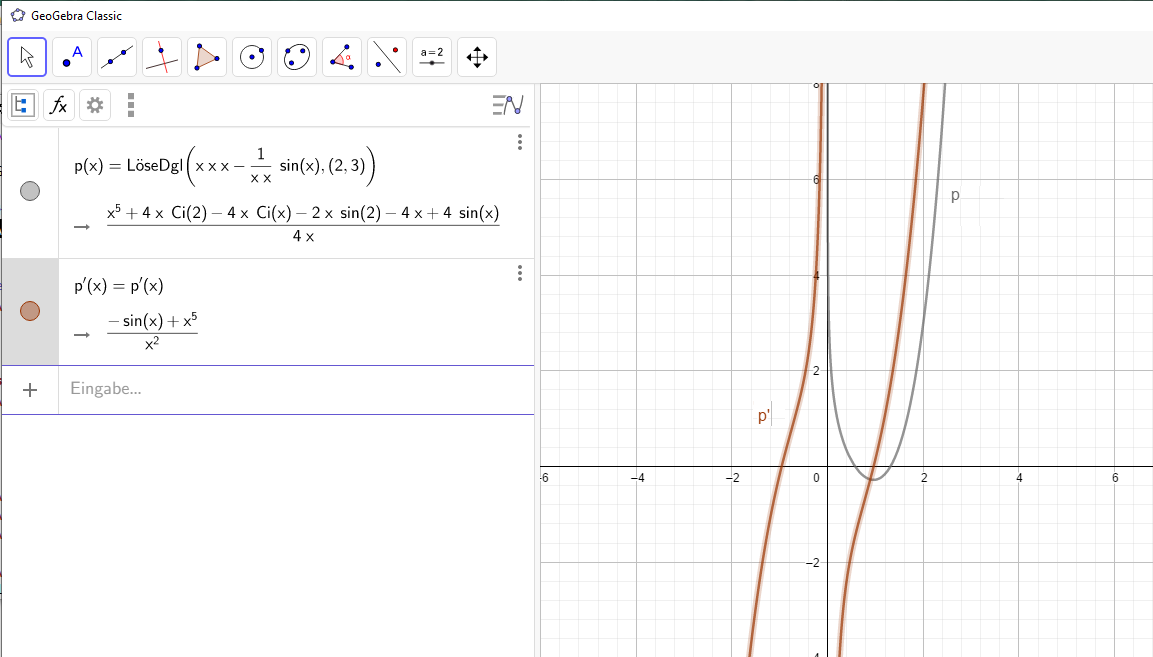
\includegraphics[width=0.9\textwidth]{../Mathematik_2/Bilder_unused/differentialgleichung_geogebra_loesungskurven.png}
%	\end{center}
%\end{exabox}

%Gibt man zu wenige Anfangsbedingungen vor wie bei \begin{verbatim} solve y''+y=0\end{verbatim} and \begin{verbatim} y(0)=1 \end{verbatim} zeigt Wolfram Alpha eine Schar m�glicher L�sungen. Das Programm klassifiziert sogar ansatzweise, um welche Art von Differentialgleichung es sich handelt. �rgerlich ist nur, dass man die Kurven, die Wolfram Alpha plottet, nicht sinnvoll weiterverarbeiten kann. Wenn man Gl�ck hat, findet Wolfram Alpha eine symbolische L�sung (also eine Formel) statt einer numerischen L�sung (also einer Wertetabelle). So eine Formel l�sst sich nat�rlich gut weiterverarbeiten.

\subsection{Explizites Euler-Verfahren}

Gegeben ist eine explizite Differentialgleichung erster Ordnung mit Anfangsbedingung:
\[
	\begin{cases}
		y(x_0) = y_0\,, \quad &x = x_0\,,\\
		y'(x) = f(y,x)\,, \quad & x>x_0\,.
	\end{cases}
\]
Gesucht ist die Funktion $y(x)$ f�r $x\geq x_0$. Der Wert von $y(x_0)$ ist vorgegeben. Wenn man in $x$ nun ein kleines St�ckchen $h$ weitergeht, also zu $x=x_0+h$, kennt man f�r sehr kleines $h$ die �nderung von $y$ in guter N�herung und kann damit sagen:
\[
	y(x_0+h) \approx y_1:= y_0 + h\cdot f(y_0,x_0)
\]

Nun kann man sch�tzen, was $y$ sein soll, wenn man noch einen Schritt $h$ weitergeht:
\[
	y(x_1+h) \approx y_2:= y_1 + h\cdot f(y_1,x_1)\,.
\]

Und nach $k+1$ Schritten
\[
	y(x_{k}+h) \approx y_{k+1}:= y_k + h\cdot f(y_k,x_k)\,.
\]

Dies ist das explizite Euler-Verfahren.
\begin{exabox}{Explizites Euler-Verfahren f�r Differentialgleichung erster Ordnung}{ }
	\begin{minipage}{0.35\textwidth}
		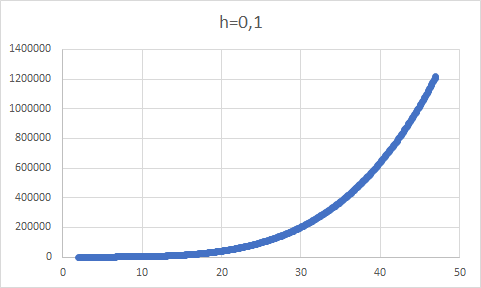
\includegraphics[width=\textwidth]{../Mathematik_2/Bilder/eulerverfahren_schrittweite_0_1.png}
\end{minipage}
	\hfill
	\begin{minipage}{0.5\textwidth}
		Anfangswertproblem:
\[ \begin{cases}
		y(2)  = 3\,, \quad &x=2\,,\\[1ex]
		y'(x) = x^3- x^{-2} \sin(y)\,, \quad &x>2\,.
	\end{cases}
\]
Iterationsvorschrift Euler-Verfahren:
\[
		y_{k+1}= y_k + h\cdot ( x_{k}^3- x_k^{-2} \sin(y_k) )\,.
\]
\end{minipage}
\end{exabox}

Wenn man die Schrittweite $h$ halbiert, verdoppelt sich die Zahl der Schritte, um einen bestimmten $x$-Wert von $x_0$ aus zu erreichen. Andererseits halbiert sich dabei ungef�hr der Fehler der N�herung.
	\begin{center}
		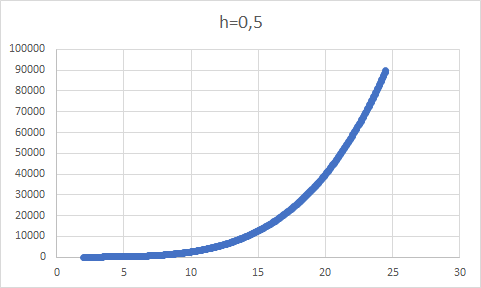
\includegraphics[width=0.4\textwidth]{../Mathematik_2/Bilder/eulerverfahren_schrittweite_0_5.png} \hspace{0.5cm}
		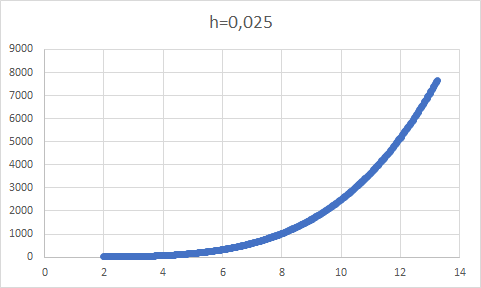
\includegraphics[width=0.4\textwidth]{../Mathematik_2/Bilder/eulerverfahren_schrittweite_0_025.png} \\
		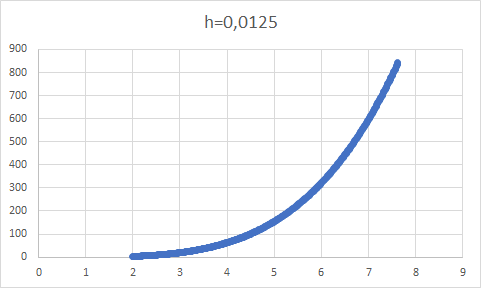
\includegraphics[width=0.4\textwidth]{../Mathematik_2/Bilder/eulerverfahren_schrittweite_0_0125.png} \hspace{0.5cm}
		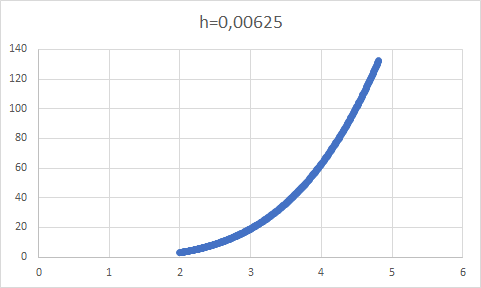
\includegraphics[width=0.4\textwidth]{../Mathematik_2/Bilder/eulerverfahren_schrittweite_0_00625.png}
\end{center}

Das st��t allerdings an eine Grenze, wenn die Schrittweite $h$ zu klein wird: Dann addiert man in dem Iterationsschritt Zahlen in sehr unterschiedlicher Gr��enordnung, so dass die Rundungsfehler �berhand nehmen. Erinnern Sie sich daran, dass man Nachkommastellen verlieren kann, wenn man normal gro�e Zahlen mit kleinen Zahlen addiert:
\[
	13 + 0,000000001\cdot 42 = 13,00000000\textcolor{blue}{42\cdots}\,.
\]
Das explizite Euler-Verfahren kann also fehlerhaft sein. Das ist eine numerische Instabilit�t. Diese Instabilit�t kann man vermeiden, wenn man das implizite Euler-Verfahren betrachtet.


\subsection{Andere L�ser f�r Differentialgleichungen erster Ordnung}

Um das $y(x)$ zu einem vorgegebenen $x$ sehr genau zu bestimmen und auch noch schnell zu rechnen, ben�tigt man deshalb Verfahren, die mit recht groben Schrittweiten $h$ auskommen.

Ein g�ngiges Verfahren ist das Runge-Kutta Verfahren von vierter Appoximationsordnung. Wenn man hier die Schrittweite $h$ halbiert, sinkt der Fehler etwa auf ein Sechzehntel. Allerdings muss man die Funktion $f$ dazu pro Schritt viermal auswerten.\marginpar{\small Aufgabe}
\begin{theorembox}{Runge-Kutta Verfahren vierter Ordnung}{ }
	Anfangswertproblem
	\[
		\begin{cases}
			y(x_0) = y_0 \,,\quad &x = x_0\,,\\
			y'(x) = f(y(x),x)\,,\quad &x> x_0\,.
	\end{cases}
\]
	Iterationsvorschrift Runge-Kutta-Verfahren:
	\[
		y_{k+1} = y_k + h\cdot \left( \frac16 k_1 + \frac13 k_2 + \frac13 k_3 + \frac16 k_4 \right)\,,
	\]
	mit
	\begin{eqnarray*}
		k_1 &=& f(y_k,x_k)\,,\\
		k_2 &=& f(y_k + \displaystyle{\frac{h}{2}} k_1,x_k + \displaystyle{\frac{h}{2}})\,,\\
		k_3 &=& f(y_k + \displaystyle{\frac{h}{2} k_2}, x_k + \displaystyle{\frac{h}{2}})\,,\\
		k_4 &=& f(y_k + h k_3, x_k + h)\,.
	\end{eqnarray*}
\end{theorembox}

Neben  der  Genauigkeit  von $y(x)$ zu  einem  vorgegeben $x$ kann  man  auch  das asymptotische Verhalten f�r $x\to \infty$ untersuchen: Die gen�herte L�sung soll nicht explodieren. Hierzu kann man implizite L�ser einsetzen.  Die Iteration beim implizite Euler-Verfahren lautet beispielsweise:
\[
\textcolor{blue}{y_k} = y_{k-1} + h\cdot f(\textcolor{blue}{y_k}, x_{k-1})\,.
\]
Anders als beim expliziten Verfahren, ist ein Gleichungssystem zu l�sen\randverweis{MA1-determinante-und-inverse} - das ist der Preis den man f�r numerische Stabilit�t zu zahlen hat.\marginpar{\small Aufgabe}

	\noindent Bemerkungen:
	\begin{itemize}
		\item Implizite L�ser sind hilfreich beim Umgang mit steifen [stiff] Systemen. So hei�en Systeme von Differentialgleichungen, in denen sehr verschieden schnelle Abklingverhalten gemischt werden. Die Anteile mit dem schnellen Abklingverhalten erzwingen gegebenenfalls eine entsprechend kleine Schrittweite.
	\end{itemize}

\subsection{Symplektische Verfahren f�r Differentialgleichungen zweiter Ordnung}

Gerade in der Mechanik ist man an Differentialgleichungen zweiter Ordnung interessiert. Man kann sich hier die symplektische Struktur der Differentialgleichungen der Mechanik zu Nutze machen.

Betrachten wir beispielsweise ein unged�mpftes Pendel der Masse $m$ mit Federkonstante $D>0$.
\begin{exabox}{Explizites Euler-Verfahren f�r System erster Ordnung}{ }
	\begin{minipage}{0.45\textwidth}
		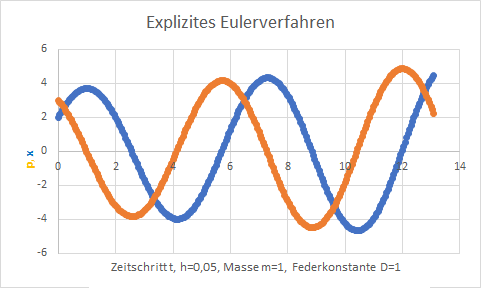
\includegraphics[width=\textwidth]{../Mathematik_2/Bilder/federpendel_explizites_eulerverfahren.png}
\end{minipage}
	\hfill
	\begin{minipage}{0.5\textwidth}
		Anfangswertproblem:
\[
	\begin{cases}
		x(t_0)=x_0\,, \quad &t=t_0\,, \\[1ex]
		p(t_0)=p_0\,, \quad &t=t_0\,,\\[2ex]
		\dot x(t) = \displaystyle{\frac{p(t)}{m}}\,, \quad &t>t_0\,,\\[1ex]
		\dot p(t) =  -D\cdot x(t)\,, \quad &t>t_0\,.
\end{cases}
 \]
Iterationsvorschrift Euler-Verfahren:
\[
	\left( \begin{array}{c} x_{k+1} \\ p_{k+1} \end{array}\right) := \left( \begin{array}{c} x_k \\ p_k \end{array}\right) + h \left( \begin{array}{c} p_k/m \\ D\cdot x_k\end{array}\right)\,.
\]
\end{minipage}
\end{exabox}
Aus der Abbildung ist ersichtlich, dass das explizite Eulerverfahren eine unphysikalische L�sung produziert: die \underline{Amplitude der Schwingung}\randverweis{MA1-trigonometrische-funktionen} wird immer gr��er!

Witzigerweise stellt sich heraus, dass der L�ser wesentlich besser funktioniert, wenn man das neue $x$ in die Gleichung f�r $p$ einsetzt - oder umgekehrt. So ergibt sich das symplektische Euler-Verfahren:
\begin{exabox}{Symplektisches Verfahren f�r ein System erster Ordnung}{}
	\begin{minipage}{0.45\textwidth}
		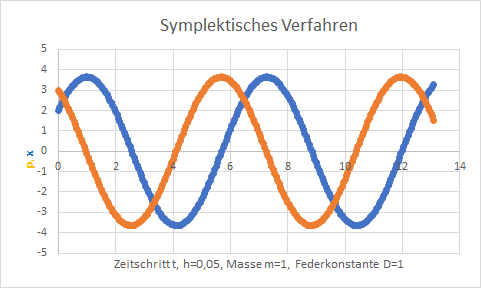
\includegraphics[width=\textwidth]{../Mathematik_2/Bilder/federpendel_symplektisches_verfahren.png}
\end{minipage}
	\hfill
	\begin{minipage}{0.5\textwidth}
		Anfangswertproblem:
\[
	\begin{cases}
		x(t_0)=x_0\,, \quad &t=t_0\,, \\[1ex]
		p(t_0)=p_0\,, \quad &t=t_0\,,\\[2ex]
		\dot x(t) = \displaystyle{\frac{p(t)}{m}}\,, \quad &t>t_0\,,\\[1ex]
		\dot p(t) =  -D\cdot x(t)\,, \quad &t>t_0\,.
\end{cases}
\]
Iterationsvorschrift symplektisches Verfahren:
\[
	\left( \begin{array}{c} \textcolor{blue}{x_{k+1}} \\ p_{k+1} \end{array}\right) := \left( \begin{array}{c} x_k \\ p_k \end{array}\right) + h \left( \begin{array}{c} p_k/m \\ D\cdot \textcolor{blue}{x_{k+1}}\end{array}\right)\,.
\]
\end{minipage}
\end{exabox}

 \newpage % 16 Numerische Lösung von Differentialgleichungen OPTIONAL % VPL Matlab
%\setcounter{exercise}{0} 
\ifintegriereaufgaben
\section*{Numerische Verfahren Aufgaben}\label{MA2-numerische-loesung-von-differentialgleichungen-aufgaben}
Erkl�rungen und Beispiele, die zur Bearbeitung der Aufgaben hilfreich sind, finden Sie im Skript\wennreferenzvorhanden{MA2-numerische-loesung-von-differentialgleichungen}{ (Abschnitt \abschnittsverweis{MA2-numerische-loesung-von-differentialgleichungen})} und, falls Sie nicht weiterkommen, dann schauen Sie \hyperref[MA2-numerische-loesung-von-differentialgleichungen-loesungen]{hier}.
\else
\section{Numerische Verfahren Aufgaben}\label{MA2-numerische-loesung-von-differentialgleichungen-aufgaben}

Regeln und Beispiele zu diesen Aufgaben finden Sie im Skript. Die L�sungen finden Sie \hyperref[MA2-numerische-loesung-von-differentialgleichungen-loesungen]{hier}.
\fi

\begin{exercisebox}[Explizites Euler Verfahren] %HMI 3 Blatt 4 Aufg. 4
	Berechnen Sie f�r das Anfangswertproblem
	\[
		\begin{cases}
			y(0) = 1\,,\quad & x=0\,,\\
			y' = x^2+y\,,\quad & x\not=0\,
		\end{cases}
	\]
	eine N�herungsl�sung f�r $y(2)$. Die N�herungsl�sung soll mit Hifle des Eulerschen Polygonzugverfahrens zur Schrittweite $h=1/4$ hergeleitet werden. L�sen Sie das Anfangswertproblem exakt und bestimmen Sie den relativen Fehler der Approximation f�r $x =2$.
\end{exercisebox}

\begin{exercisebox}[Verbessertes Euler Verfahren] %HMI 3 Blatt 6 Aufg. 1
	Eine Verbesserung des expliziten Euler Verfahrens lautet
	\[
		\begin{cases}
			k_1 = f(x_k, y_k)\,,\\
			k_2 = f(x_k+\frac{h}{2}, y_k + \frac{h}{2}k_1)\,,\\
			y_{k+1} =  y_k + hk_2\,.
		\end{cases}
	\]
	\begin{itemize}
		\item[(a)] Verdeutlichen Sie graphisch die Funktionsweise des Verfahrens.
		\item[(b)] Bestimmen Sie f�r das Anfangswertproblem aus der ersten Aufgabe die Approximation f�r $x=2$ zur Schrittweite \(h=1/4\) und bestimmen Sie den relativen Fehler zur exakten L�sung.
		\item[(c)] Betrachten Sie das Anfangswertproblem
	\[
		\begin{cases}
			y(0) = y_0\,,\quad & x=0\,,\\
			y' = -2at\,,\quad & x\not=0\,.
		\end{cases}
	\]
	�berzeugen Sie sich davon, dass die verbesserte Polygonzugmethode das Anfangswertproblem zu unterschiedlichen Werten von \(a = 2\) und Anfangswerten \(y_0 = \sqrt(2)\) exakt l�st (numerisch!). Was k�nnen Sie daraus schlie�en?  	 % Blatt 7 Aufg.1
	\end{itemize}
\end{exercisebox}

\begin{exercisebox}[Explizites Euler Verfahren] %HMI 3 Blatt 7 Aufg. 3
	Betrachten Sie ein explizites Euler-Verfahren f�r das Anfangswertproblem
	\[
		\begin{cases}
			y(0) = 0\,,\quad & x=0\,,\\
			y' = 4x^2-7x+3\,,\quad & x\not=0\,.
		\end{cases}
	\]
	\begin{itemize}
		\item Berechnen Sie die exakte L�sung  $\Phi$ des Anfangswertproblems.
		\item Berechnen Sie bei vorgegebener Schrittweite $h$ mit dem Euler-Verfahren N�herungswerte $y_k$ f�r $\Phi(x_k)$ und explizit die Fehler $\epsilon(x_k,h) = y_k - \Phi(x_k)$ mit $x_k = kh$.
		\item Zeigen Sie, dass der Fehler $\epsilon(x_k,h) = y_k - \Phi(x_k)$ bei festem $x$ f�r $h\to 0$ gegen Null konvergiert.
	\end{itemize}
\end{exercisebox}

\begin{exercisebox}[Implizites Euler Verfahren] %HMI 3 Blatt 7 Aufg. 1
	Betrachten Sie das Anfangswertproblem
	\[
		\begin{cases}
			y(0) = y_0\,,\quad & x=0\,,\\
			y' = -2at\,,\quad & x\not=0\,.
		\end{cases}
	\]
	Bestimmen Sie f�r das implizite Eulerverfahren den lokalen Diskretisierungsfehler
	\[
		\tau(t,h) := \frac1h \left( y(t_{k+1}) - y_{k+1} \right)
	\]
\end{exercisebox}

%\subsection{Praxis}
%\begin{exercisebox}[Moodle] % HMI III; Blatt 12, Augabe 4
%L�sen Sie das lineare Randwertproblem
%\[
%y'' - x y' +4y = x \land y(0) = 1 \land y(1) = 0 \]
%n�herungsweise mit Hilfe der Differenzenmethode, das hei�t zerlegen Sie das Intervall \([0,1]\) �quidistant mit einer Schrittweite \(h=0.2\) und approximieren Sie die auftretenden Ableitungen durch die Differentzenquotienten
%\begin{eqnarray*}
%	y'(x) &\approx& \frac{ y(x+h) - y(x-h) }{2h} \textnormal{ zentrale Differenz}\\
%	y''(x) &\approx& \frac{ y(x+h) - 2y(x) + y(x-h) }{h^2} \textnormal{ zweite Differenz}
%\end{eqnarray*}
%\end{exercisebox}

%\subsection{Praxis}
%\begin{mybox}[MC Differentialgleichungen]
%\begin{itemize}
%	\item Welcher L�sungsansatz ?
%\end{itemize}
%\end{mybox}


%https://me-lrt.de/anfangswertproblem-implizites-eulerverfahren !!!!

%
 \newpage
\setcounter{def}{0} \setcounter{satz}{0} \setcounter{exa}{0} 
\section{Differentialgleichungen mit trennbaren Variablen (+)}\label{MA2-trennbare-differentialgleichungen}

\begin{table}[H]
  \centering
  \begin{tabularx}{\textwidth}{@{}>{\raggedright\arraybackslash}X r@{}}
    \toprule
    \multicolumn{2}{c}{\textbf{�bersicht �ber Lernziele und Voraussetzungen}} \\
    \midrule
    \textbf{Lernziele} & \\[.5\normalbaselineskip]
    \tabitem Differentialgleichungen mit trennbaren Variablen durch Separation der Variablen l�sen & \\
    \tabitem Anfangswertprobleme dieses Typs vollst�ndig bestimmen & \\[.5\normalbaselineskip]
    \midrule
    \textbf{Voraussetzungen} &  \\[.5\normalbaselineskip]
    \tabitem Integrale sicher berechnen k�nnen & \abschnittsverweis{MA2-integrationsregeln}  \\[.5\normalbaselineskip]
    \bottomrule
  \end{tabularx}
\end{table}

\noindent \ifintegriereaufgaben Die �bungsaufgaben zum Thema finden Sie \hyperref[MA2-trennbare-differentialgleichungen-aufgaben]{hier}.
\vspace{0.3cm}
\hrule
\fi


\subsection{Trennbare Variablen}

Die sogenannte "\,Trennung der Variablen"\, [separation of variables] ist ein beliebter Trick, um Anfangswertprobleme erster Ordnung (und nur erster Ordnung) zu l�sen. Differentialgleichungen erster Ordnung haben trennbare Variablen [separable variables], wenn gilt:
\begin{defbox}{Differentialgleichung mit trennbaren Variablen}{ }
	Die Differentialgleichung l��t sich eine Form bringen, in der
	\begin{itemize}
		\item auf der linken Seite das Produkt der Ableitung $y'$ mit einer Funktion $h$ steht, wobei $h$ nur von $y$ abh�ngt,
		\item auf der rechten Seite nur eine Funktion $f$ der unabh�ngigen Variable $x$ auftaucht.
	\end{itemize}
	Schematisch sieht sie dann so aus:
	\[ h(y(x)) \cdot y'(x) = f(x)\,.\]
\end{defbox}

\subsection{L�sungsstrategie}

Die grunds�tzliche Idee ist beide Seiten der Gleichung zu integrieren und die \underline{Substitutionsregel}\randverweis{MA2-integrationsregeln} anzuwenden. Die Substitution lautet
\[
	s = y(x) \Rightarrow \mathrm{d}s = y'(x)\, \mathrm d x\,.
\]
Anstatt $s$ schreibt man einfach $y$, also
\[
	y = y(x) \Rightarrow \mathrm{d}y = y'(x)\, \mathrm d x\,. \quad(*)
\]

Wir schauen uns das Vorgehen f�r das folgende Anfangswertproblem an:
\[
\begin{cases}
	y(3) =  7\,, \quad & x=3\,,\\[1ex]
	\displaystyle{e^{y(x)}} y'(x) = x^5, \quad & x > 3\,.
\end{cases}
\]
Wir integrieren beide Seiten der Differentialgleichung vom Startpunkt $(x,y)=(3,7)$ zu einem beliebigen Endpunkt $(x_1,y_1)$ und integrieren durch Substitution:
\begin{eqnarray*}
	\begin{array}{l rcl c rcl}
		& \displaystyle{\int\limits_{3}^{x_1}} e^y \displaystyle{\frac{\mathrm{d}y}{\mathrm{d}x}}\,\mathrm{d}x &=& \displaystyle{\int\limits_{3}^{x_1}} x^5 \, \mathrm{d}x  &\stackrel{\displaystyle{ (*)}}{\Leftrightarrow} & \displaystyle{\int\limits_{7}^{y_1}} e^y \,\mathrm{d}y &=& = \displaystyle{\int\limits_{3}^{x_1}} x^5 \, \mathrm{d}x \\[2ex]
		& & &  &\Leftrightarrow  & \Big[ \displaystyle{e^{y}}\Big]_{7}^{y_1} &=& \Big[ \displaystyle{\frac16 x^6}\Big]_{3}^{x_1} \\
		&&&&\Leftrightarrow  & \displaystyle{e^{y_1} - e^{7}} &=& \displaystyle{7\frac{x_1^6}{6} - \frac{3^6}{6}}
\end{array}
		\end{eqnarray*}
Und es ergibt sich die L�sung:
\[
 y_1 =\ln\left( e^7 + \frac{x_1^6}{6} - \frac{3^6}{6} \right) \,.
\]

\noindent Bemerkungen:
\begin{itemize}
	\item Das Aufl�sen nach $y_1$ im letzten Schritt kann problematisch sein - denken Sie an den Definitionsbereich der \underline{Umkehrfunktionen}\randverweis{MA1-eigenschaften-von-funktionen}.
	\item Der Name der L�sungmethode kommt daher, dass man die Differentialgleichung formal umformen kann zu
		\[
			e^y y' = x^5 \Leftrightarrow e^y \frac{\mathrm{d}y}{\mathrm{d}x} = x^5 \Rightarrow  e^y \mathrm{d}y = x^5 \mathrm{d}x\,.
	\]
In dieser Form sind die Variablen $x$ und $y$ getrennt und dann auf beiden Seiten von $(x,y)=(3,7)$ bis $(x_1,y_1)$ integriert:
			\[
			\int\limits_{7}^{y_1} e^y \,\mathrm{d}y = \int\limits_{3}^{x_1} x^5 \, \mathrm{d}x\,.
		\]
	\item Manche Leute verzichten auf die Anfangs- und Endwerte und schreiben unbestimmte Integrale, um die allgemeine L�sung der Differentialgleichung zu erhalten. Aber dann darf man die Integrationskonstante nicht vergessen:
			\[
			\int e^y \,\mathrm{d}y = \int x^5 \, \mathrm{d}x \Leftrightarrow e^y  = \frac{x^6}{6} + c\,.
		\]
	Die allgemeine L�sung lautet mit $C = \ln(c)$ also
		\[
			y(x)  = C\cdot \ln\left(\frac{x^6}{6}\right)\,.
	\]
\end{itemize}

\begin{exabox}{Nichtlinear von erster Ordnung}{ }
Anfangswertproblems:
	\[
		\begin{cases}
			y(0) = 1\,, &\quad x=0\,,\\
			y'(x)+y^2(x)  = 0\,, &\quad x>0\,.
		\end{cases}\]
Trennung der Variablen:
\begin{eqnarray*}
y'+y^2 = 0 \Leftrightarrow \frac{\mathrm{d}y}{\mathrm{d}x}  -y^2 &=&  0  \\
\stackrel{y\not=0}{\Leftrightarrow} \frac{1}{y^2}\cdot \frac{\mathrm{d}y}{\mathrm{d}x} &=& -1 \\
\Leftrightarrow \frac{1}{y^2}\cdot \mathrm{d}y &=& -\mathrm{d}x
\end{eqnarray*}
Integration:
\[
\int \frac{1}{y^2}\,\mathrm{d}y = -\int\,\mathrm{d}x  \stackrel{x\not=C}{\Leftrightarrow} y = \frac{1}{x-C} \,.
\]
Bestimmung der Integrationskonstanten:
\[ y(0) = -\frac{1}{C} \stackrel{!}{=} 1 \Leftrightarrow C = -1 \,.\]
L�sung:
\[ y(x) = \frac{1}{x+1}\,.\]
\end{exabox}

Bei den folgenden Differentialgleichungen f�hrt eine Substitution auf eine Form, die mit dem Schema dieses Abschnitts zu l�sen ist:

	\begin{center}
		\begin{tabular}{c|c|c}
			vorher & Substitution & nachher \\ \hline
			$y' =\tilde h(ax+by+c)$ & $ u = ax+by+c$ & $u' = a+b \tilde h(u)$ \\
			\hline
			$y' =\tilde h \left(\displaystyle{\frac{y}{x}}\right)$ & $ u = \displaystyle{\frac{y}{x}}$ & $u' = \displaystyle{\frac{\tilde h(u) - u}{x}}$ \\
		\end{tabular}
	\end{center}
 \newpage % 17 Differentialgleichungen mit trennbaren Variablen OPTIONAL
%\setcounter{exercise}{0} 
\ifintegriereaufgaben

\section*{Differentialgleichungen mit trennbaren Variablen Aufgaben}\label{MA2-trennbare-differentialgleichungen-aufgaben}
Erkl�rungen und Beispiele, die zur Bearbeitung der Aufgaben hilfreich sind, finden Sie im Skript\wennreferenzvorhanden{MA2-trennbare-differentialgleichungen}{ (Abschnitt \abschnittsverweis{MA2-trennbare-differentialgleichungen})} und, falls Sie nicht weiterkommen, dann schauen Sie \hyperref[MA2-trennbare-differentialgleichungen-loesungen]{hier}.
\else
\section{Differentialgleichungen mit trennbaren Variablen Aufgaben}\label{MA2-trennbare-differentialgleichungen-aufgaben}

Regeln und Beispiele zu diesen Aufgaben finden Sie im Skript. Die L�sungen finden Sie \hyperref[MA2-trennbare-differentialgleichungen-loesungen]{hier}.
\fi

\begin{exercisebox}[Trennung der Variablen] %Papula IV, Abschnitt 2, Aufgabe 4
L�sen Sie die folgenden Differentialgleichungen durch Trennung der Variablen:
\begin{eqnarray*}
	\begin{array}{ll}
		(a)\; y' = \displaystyle{\frac{y^2}{x^2}}, \; x\in (0,\infty) \quad \quad & (b)\; y'= \displaystyle{\frac{x\cdot y}{1+x^2}} \\
			(c)\; y' = (1-y)^2 \quad \quad & (d)\; y'\cdot \sin(y)= -x,  \; y\in (0,\pi)
		\end{array}
\end{eqnarray*}
\end{exercisebox}


\begin{exercisebox}[Inhomogenit�t] %Papula IV, Abschnitt 2, Aufgabe 16
	L�sen Sie folgenden Anfangswertprobleme durch Variation der Konstanten:
\begin{eqnarray*}
	\begin{array}{l c l}
		(a) \quad  xy'-y = x^2 \cdot \cos(x)  & \land & y(\pi) = 2\pi \\[1ex]
		(b) \quad  xy'+y = \ln(x) & \land & y(1) = 1\\[1ex]
		% (b) Papula \quad  y'+\tan(x)\cdot y = 5\cdot \sin(2x)  & \land & y(3\pi) = 2 \\[1ex]
		(c) \quad  y'-\tan(x)\cdot y = 5\cdot \sin(2x)  & \land & y(3\pi) = 2 % Ver�nderung
	\end{array}
\end{eqnarray*}
\small{Hinweis zur Integration in Aufgabenteil (c): benuzten Sie ein Additionstheorem! }
\end{exercisebox}

\begin{exercisebox}[Substitution] %Papula IV, Abschnitt 2, Aufgabe 3
	L�sen Sie das folgende Anfangswertproblem:
	$
	y' = \displaystyle{\frac{y}{x} } +\displaystyle{\frac{x}{y} }, \quad y(1) = \sqrt{2}\,.
	$
\end{exercisebox}

\begin{exercisebox}[Substitution] %Papula IV, Abschnitt 2, Aufgabe 2
	L�sen Sie die folgenden Differentialgleichungen mit Hilfe einer geeigneten Substitution. Schlagen Sie die auftretenden Integrale gegebenenfalls in einer Formelsammlung nach:
\begin{eqnarray*}
	\begin{array}{ll}
		(a)\; y' = \displaystyle{\frac{y}{x} + 4}, \; x\in (0,\infty) \quad \quad & (b)\; y'= (x+y+1)^2 \\
		(c)\; y' = \displaystyle{\frac14} + \displaystyle{\frac{y^2}{x^2}}, x\in (0,\infty) \quad \quad & (d)\; y' = \sin(\frac{y}{x}) + \frac{y}{x},  \; x\in (0,\infty)
		\end{array}
\end{eqnarray*}
\end{exercisebox}

\begin{exercisebox}[Logistisches Wachstum]
	Die Anzahl der von einem Virus infizierten Personen $x(t)$ zum Zeitpunkt $t$ in einer Bev�lkerung der Gr��e $N$ kann folgenderma�en modelliert werden: Pro Tag habe jede Person $k>0$ zuf�llige Kontakte, wobei der Virus bei jedem Kontakt �bertragen wird.
	\begin{itemize}
		\item[(a)] Wie viele nicht infizierte Personen gibt es in Abh�ngigkeit von $x(t)$ zum Zeitpunkt $t$? Wie gro� ist der Anteil der nicht infizierten Personen zum Zeitpunkt $t$?
		\item[(b)] Wie viele Personen trifft eine infizierte Person in einer kleinen Zeitpanne $[t, t+\Delta t]$? Wieviele nicht infizierte Personen trifft eine infizierte Person in $[t, t+\Delta t]$?
		\item[(c)] Wie viele Kontakte von infizierten Personen mit nicht infizierten Personen gibt es insgesamt in $[t,t+\Delta t]$? Wie viele Personen werden daher in $[t, t+\Delta t]$ neu angesteckt?
		\item[(d)] Dr�cken Sie $x(t+\Delta t)$ durch $x(t)$ und die Anzahl der neu infizierten Personen in $[t, t+\Delta t]$ aus.
	\item[(e)] F�hren Sie den Grenzwert $\Delta t\to 0$ aus, um eine Differentialgleichung zu erhalten. Wie lautet die L�sung des zugeh�rigen Anfangswertproblemes wenn $x(0)=1$ war?
\end{itemize}
\end{exercisebox}

\begin{exercisebox}[Differentialgleichungen erster Ordnung] %Papula IV, Abschnitt 2, Aufgabe 20
	\small{L�sen Sie folgenden Differentialgleichungen mit Hilfe einer geeigneten Methode:}
\begin{eqnarray*}
	\begin{array}{ll l }
		(a)\; y' = x(y^2+1) \;  & (b)\; y'= y\cdot \sin(x) \; & (c)\; y' = xy \\
		(d)\; xy' + y = 2\ln(x) \; (e)\; y' = 5x^4(y+1) \; & (f)\; y' - 5y = 2\cos(x) - \sin(3x)
		\end{array}
\end{eqnarray*}
\end{exercisebox}

%\subsection{Praxis}

%\begin{exercisebox}[Moolde Eindimensionaler harmonischer Oszillator] % HMI III, Blatt 11, Aufgabe 1
%	Die Bewegung eines eindimensionalen harmonischen Oszillators wird durch die Differentialgleichung
%	\[ \ddot x = -2x \] beschrieben. Bestimmen Sie:
%	\begin{itemize}
%		\item[(a)] das zugeh�rige lineare Gleichungssystem erster Ordnung.
%		\item[(b)] die Differentialgleichung $f(x,v,v') = 0$ der Phasenbahnb,
%		\item[(c)] die allgemeine L�sung dieser Differentialgleichung und damit das Phasenportrait der Bewegung,
%		\item[(d)] die Phasenkurve f�r die Anfangswerte $x(0)=1\land \dot x(0) = -1$,
%		\item[(e)] die Skizze dieser Phasenkurve mit Umlaufsinn,
%		\item[(f)] die zugeh�rige Bahnkurve $x=x(t)$.
%	\end{itemize}
%
%\vspace{0.3cm}
%{\bf L�sung:} \newline
%\begin{itemize}
%	\item[(a)]
%		\[ \dot x = y \land \dot y = -2x \Rightarrow \left( \begin{array}{c} \dot x \\\dot y \end{array}\right) = \left( \begin{array}{cc} 0 & 1 \\ -2 & 0\end{array}\right) \left( \begin{array}{c} x \\ y \end{array}\right) \,.
%		\]
%	\item[(b)] \[ \frac{\mathrm{d} y}{\mathrm{d} x} = \frac{-2x}{y} \Rightarrow y' = \frac{-2x}{y} \Rightarrow f(x, y, y') = y'\cdot y + 2x = 0\]
%	\item[(c)] (Ellipse) \[ y' = \frac{-2x}{y} \Rightarrow y\mathrm{d}y = -2x \mathrm{d}x \Leftrightarrow \frac12 y^2 = - x^2 + c \Leftrightarrow \frac{1}{2c}y^2 + \frac{1}{c} x^2 = 1 \,.
%		\]
%	\item[(d)] Bestimmung der Integrationskonstante: \[x(0) = 1 \land y(0) = \dot x(0) = -1 \Rightarrow c = \frac32\]
%		Phasenkurve: \[ \frac13 y^2+ \frac23 x^2 = 1 \,.\]
%		Skizzte: Elipse, die im Uhrzeigersinn durchlaufen wird. Tangentialvektor $\boldsymbol t = \left( \dot x , \dot y\right)^\intercal = (0,-2\sqrt{3/2})^\intercal $.
%\end{itemize}
%\end{exercisebox}

 \newpage

\chapter{Laplacetransformation}
\section*{Leitidee}
Die Laplacetransformation erm�glicht es, Differentialgleichungen in algebraische Gleichungen zu �berf�hren. Dynamische Prozesse werden damit aus dem Zeitbereich in einen Transformationsraum �berf�hrt, in dem ihre Struktur leichter analysiert werden kann.

Auf diese Weise wird die Untersuchung dynamischer Systeme auf algebraische Operationen zur�ckgef�hrt.  Die Laplacetransformation wird deshalb zu einem zentralen Werkzeug der Systemtheorie.

\bigskip
\etocsettocstyle{\section*{Inhalt dieses Kapitels}}{}
\localtableofcontents
\newpage

\setcounter{def}{0} \setcounter{satz}{0} \setcounter{exa}{0} \section{Laplacetransformation}\label{MA2-laplacetransformation}

\begin{table}[H]
  \centering
  \begin{tabularx}{\textwidth}{@{}>{\raggedright\arraybackslash}X r@{}}
    \toprule
    \multicolumn{2}{c}{\textbf{�bersicht �ber Lernziele und Voraussetzungen}} \\
    \midrule
    \textbf{Lernziele} & \\[.5\normalbaselineskip]
    \tabitem die Laplace-Transformierte geeigneter Funktionen berechnen & \\
    \tabitem die Wirkung der Laplace-Transformation auf Ableitungen als Regel anwenden & \\[.5\normalbaselineskip]
    \midrule
    \textbf{Voraussetzungen} &  \\[.5\normalbaselineskip]
    \tabitem uneigentliche Integrale berechnen k�nnen & \abschnittsverweis{MA2-integration}\\
    \tabitem Ableitungen sicher berechnen k�nnen & \abschnittsverweis{MA1-ableitungsregeln} \\[.5\normalbaselineskip]
    \bottomrule
  \end{tabularx}
\end{table}

\noindent \ifintegriereaufgaben Die �bungsaufgaben zum Thema finden Sie \hyperref[MA2-laplacetransformation-aufgaben]{hier}.
\vspace{0.3cm}
\hrule
\fi

\subsection{Definition}

In vielen Anwendungen � insbesondere in der Regelungstechnik �
interessiert man sich f�r Vorg�nge, die zu einem bestimmten Zeitpunkt beginnen.
Ein System befindet sich im Ruhezustand und wird bei $t=0$
durch eine St�rung oder ein Eingangssignal angeregt.

Mathematisch f�hrt dies auf Anfangswertprobleme der Form
\[
	m \ddot x + \rho \dot x + D x = u(t),
	\qquad x(0)=x_0, \quad \dot x(0)=v_0.
\]

Die Schwierigkeit besteht darin, dass Ableitungen auftreten.
Ableitungen machen Gleichungen kompliziert �
Multiplikationen dagegen sind einfach.

\medskip

Die zentrale Idee der Laplace-Transformation lautet daher:

\begin{center}
	\emph{Man sucht eine Darstellung, in der Ableitungen zu Multiplikationen werden.}
\end{center}

Genau das leistet die Laplace-Transformation.
Sie ordnet einem Signal $y(t)$ eine Funktion $Y(s)$ zu,
in der Differentiation im Zeitbereich
zu einer algebraischen Operation im Bildraum wird.

\medskip

Dabei betrachtet man nur Zeiten $t \ge 0$.
Vor dem Zeitpunkt $t=0$ sei das System im Ruhezustand,
man setzt also meist $y(t)=0$ f�r $t<0$.

Die Laplace-Transformierte eines Signals
$y:[0,\infty)\to\mathbb C$ wird definiert als:
\begin{defbox}{Laplace-Transformation}{ }
	\[
		\mathcal L(y): D_Y \subset \mathbb C \to \mathbb C,
		\qquad
		s \mapsto Y(s),
		\qquad
		Y(s) := \int_0^\infty y(t)\, e^{-st}\,\mathrm d t.
	\]
\end{defbox}

\noindent Bemerkungen:
\begin{itemize}
	\item Das Integral muss nicht f�r alle $s\in\mathbb C$ existieren.
	Der Definitionsbereich $D_Y$ ist im Allgemeinen
	eine echte Teilmenge der komplexen Zahlen.

	\item Die Exponentialfunktion $e^{-st}$ wirkt f�r $\mathrm{Re}(s)>0$
	d�mpfend.
	W�chst $y(t)$ nicht schneller als eine Exponentialfunktion,
	so existiert das entstehende uneigentliche Integral.
\end{itemize}

\medskip

Man sagt: Das Signal $y(t)$ liegt im \emph{Zeitbereich}.
Seine Laplace-Transformierte $Y(s)$ liegt im \emph{Bildraum}.

Die Transformation ver�ndert nicht das physikalische System,
sondern nur seine Darstellung.
Der Perspektivwechsel macht jedoch eine entscheidende Struktur sichtbar:
Differentialgleichungen werden im Bildraum zu algebraischen Gleichungen.

\subsection*{Eigenschaften}

Was passiert, wenn man die Laplace-Transformation auf die Ableitung $\dot y$ eines Signals los l�sst?
\[
	\int\limits_0^\infty \dot y(t) \, e^{-st}\, \mathrm{d}t = \Big[ y(t) e^{-st} \Big]_0^\infty + s \int\limits_0^\infty y(t) \, e^{-st}\, \mathrm{d}t = -y(0) +s Y(s) \,.
\]
Die Ableitung wird also quasi ein Produkt - quasi, weil der Randterm noch als additive Konstante hinzukommt!\footnote{Die Fourier-Transformation der Ableitung liefert �brigens exakt ein Produkt.}\marginpar{\small Aufgabe}

In �hnlicher Weise kann man die Frage stellen, ob sich die Ableitung der Laplace-Transformierten in ein Produkt im Zeitbereich darstellt. Die Antwort ist ja. Die Formeln f�r h�here Ableitungen sind in der folgenden Box zusammengefasst:
\begin{theorembox}{Laplace-Transformierte und die Ableitung}{ }
	Die Laplace-Transformierte von \(y^{(n)}\) lautet:
	\[
		\mathcal L \left( y^{(n)}\right) (s) = s^n Y(s) - \sum\limits_{k=0}^{n-1} y^{(k)}(0) s^{n-k-1}
	\]
	Die $n$-te Ableitung der Laplace-Transformierten von \(y\) lautet:
	\[
		Y^{(n)}(s) = \mathcal L \left( (-t)^n y\right)(s)\,.
	\]
\end{theorembox}

\begin{exabox}{Laplace-Transformation von $\exp$, $\sin$ und $\cos$}{ }
	\begin{itemize}
	\item F�r $y:t\mapsto e^{\lambda t}$ mit $\lambda \in \mathbb R$ gilt
	\[
		\int\limits_0^\infty e^{\lambda t}\cdot e^{-st} \, \mathrm{d} t =
		\int\limits_0^\infty e^{ (\lambda-s) t} \, \mathrm{d} t =
	\Big[ \frac{e^{(\lambda -s ) t }}{\lambda -s}\Big]_0^\infty = \frac{1}{s-\lambda},\quad \textnormal{wenn } \mathrm{Re}(s)>\lambda\,.
	\]
	\item F�r $y:t\mapsto e^{i\omega t}$ mit $\omega \in \mathbb R$ gilt
	\[
		\int\limits_0^\infty e^{i\omega t}\cdot e^{-st} \, \mathrm{d} t =
		\int\limits_0^\infty e^{ (i\omega-s) t} \, \mathrm{d} t =
	\Big[ \frac{e^{(i\omega -s ) t }}{i\omega -s}\Big]_0^\infty = \frac{1}{s-i\omega},\quad \textnormal{wenn } \mathrm{Re}(s)>0\,.
	\]
\item F�r $y:t\mapsto \cos(\omega t)$ gilt
	\[
		\int\limits_0^\infty \cos(\omega t)\cdot e^{-st} \, \mathrm{d} t =
		  \frac{s}{s^2 + \omega^2},\quad \textnormal{wenn } \mathrm{Re}(s)>0\,.
	\]
\item F�r $y:t\mapsto \sin(\omega t)$ gilt
	\[
		\int\limits_0^\infty \sin(\omega t)\cdot e^{-st} \, \mathrm{d} t =
		  \frac{\omega}{s^2 + \omega^2},\quad \textnormal{wenn } \mathrm{Re}(s)>0\,.
	\]
	\end{itemize}
\end{exabox}

\begin{exabox}{Laplace-Transformation von Potenzfunktionen}{ }
Das Integral
\[
\int\limits_0^\infty t^n \cdot e^{-st}\,\mathrm{d}t  = \textnormal{?}
\]

Um das Integral zu l�sen ist es geschickt, den Integranden so umzuschreiben, dass eine Ableitung nach \(s\) auftaucht:
\begin{eqnarray*}
	\int\limits_0^\infty t^n \cdot e^{-st}\,\mathrm{d}t  &=& \int\limits_0^\infty (-1)^n\cdot \frac{\mathrm{d}^n}{\mathrm{d}s^n} \left( e^{-st} \right) \,\mathrm{d}t = (-1)^n\cdot \frac{\mathrm{d}^n}{\mathrm{d}s^n} \int\limits_0^\infty  e^{-st} \,\mathrm{d}t = (-1)^n\cdot \frac{\mathrm{d}^n}{\mathrm{d}s^n} \Big[ \frac{e^{-st}}{-s} \Big]_0^{\infty}\\ &=& (-1)^n \cdot \frac{\mathrm{d}^n }{\mathrm{d}s^n}\frac{1}{s}, \quad \mathrm{Re}(s) > 0\,.
\end{eqnarray*}

%Die Potenzfunktionen  mit  Exponent  $0,1,2,3,\dots$ haben  also  diese  Laplace-Transformierten:
%\begin{center}
%	\begin{tabular}{c |c | c}
%		$n$ &  $y(t)$ & $Y(s)$\\
%		\hline
%		$0$ & $1$ & $s^{-1}$ \\
%		$1$ & $t$ & $s^{-2}$ \\
%		$2$ & $t^2$ & $2 s^{-3}$ \\
%		$3$ & $t^3$ & $6 s^{-4}$ \\
%		$\vdots$ & $\vdots$ & $\vdots$ \\
%		$n$ & $t^n$ & $n! s^{-n-1}$ \\
%	\end{tabular}
%\end{center}
\end{exabox}

\begin{theorembox}{Laplace-Transformierten der Potenzfunktionen}{}
	F�r die Potenzfunktion $y: t\mapsto t^n$ mit $n\in \mathbb N^+$ existiert die Laplace-Transformierte f�r alle \(s\in \mathbb C\) mit \(\mathrm{Re}(s) >0\) und sie lautet:
\[ Y: s\mapsto n!\, \frac{1}{s^{n+1}}\,.\]
\end{theorembox}

\begin{exabox}{Zeitliche Verz�gerung}{ }
Wenn  das  Signal $y$ um  die  Zeit $a$ verz�gert  wird,  ergibt  sich  als  Laplace-Transformierte:
\[
	\int\limits_{\textcolor{blue}{a}}^\infty y(t\textcolor{blue}{-a}) e^{\displaystyle{-st}}\,\mathrm{d}t \stackrel{(*)}{=}
	\int\limits_0^\infty y(u) e^{\displaystyle{-s(u+\textcolor{blue}{a})}}\,\mathrm{d}u = e^{\displaystyle{-s\textcolor{blue}{a}}}\left( \mathcal L y\right) (s)\,.
\]
$(*)$ mit der Substitution $u=t-\textcolor{blue}{a}$, $\mathrm{d}u = \mathrm{d}t$.
\end{exabox}

\begin{exabox}{Zeitliche Beschleunigung}{ }
Wenn das Signal $y$ um den Faktor $b > 1$ beschleunigt (oder bei $b<1$ verlangsamt) wird, ergibt sich als Laplace-Transformierte:
\[
	\int\limits_{0}^\infty y(\textcolor{blue}{b}\cdot t) e^{\displaystyle{-st}}\,\mathrm{d}t \stackrel{(*)}{=} \int\limits_0^\infty y(u) e^{\displaystyle{ -\dfrac{s}{\textcolor{blue}{b}} \cdot u}} \frac{1}{\textcolor{blue}{b}}\,\mathrm{d}u = \frac{1}{\textcolor{blue}{b}}\left( \mathcal L y\right) \left( \dfrac{ s}{\textcolor{blue}{b}}\right)\,.
\]
$(*)$ mit der Substitution $u=\textcolor{blue}{b} \cdot t$, $\mathrm{d}u = \textcolor{blue}{b}\,\mathrm{d}t$.
\end{exabox}

\begin{theorembox}{Eigenschaften der Laplace-Transformation}{ }
	Die Laplace-Transformation $\mathcal L: f\mapsto \mathcal L(f)$ ist eine lineare Abblidung:
	\begin{itemize}
		\item $\mathcal L(f+g) = \mathcal L(f) + \mathcal L(g) $
		\item $\mathcal L(\lambda f) = \lambda \mathcal L(f)$
	\end{itemize}
\end{theorembox}

F�r eine kausale Verz�gerung verwenden wir die Heaviside-Funktion
\(H(t)=0\) f�r \(t<0\) und \(H(t)=1\) f�r \(t\geq0\).
Das um \(a>0\) verz�gerte Signal lautet damit \(H(t-a)f(t-a)\).

\begin{exabox}{Rechenregeln f�r die Laplace-Transformation}{ }
	Die Laplacetransformierten der Standardsignale \(f_1: t\mapsto \cos(t)\) und \(f_2: t\mapsto t\) sind gegeben:
	\[ \cos(t) \,\laplace \, \dfrac{s}{s^2+1}, \quad t \,\laplace \, \dfrac{1}{s^2}\]
	Mit Hilfe der Rechenregeln folgt:
	\[
		\begin{array}{l rclcl l}
			f:t\mapsto \cos(t) + t\; \quad & \mathcal L(f)(s) &=& \mathcal L(f_1)(s) + \mathcal L (f_2) (s) &=& \dfrac{s}{s^2+1} +\dfrac{1}{s^2}  & \textnormal{ Linearitaet} \\[2ex]
			f:t\mapsto H(t-3)\cos(t-3)\; \quad & \mathcal L(f)(s) &=& e^{-3\, s} \cdot \mathcal L(f_1)(s) &=& e^{-3\, s}\dfrac{s}{s^2+1} & \textnormal{ Verz�gerung} \\[2ex]
			f:t\mapsto \cos(4t)\; \quad & \mathcal L(f)(s) &=& \dfrac14 \,\mathcal L (f_1)\left( \dfrac{s}{4} \right) &=& \dfrac14 \dfrac{\dfrac{s}{4}}{\left( \dfrac{s}{4}\right)^2+1} = \dfrac{s}{s^2+16}  & \textnormal{ Beschleunigung} \\[2ex]
			f:t\mapsto \cos(4t) - t\; \quad & \mathcal L(f)(s) &=&  \dfrac14 \, \mathcal L(f_1)\left( \dfrac{s}{4}\right)- \mathcal L (f_2)(s)  &=& \dfrac{s}{s^2+16}-\dfrac{1}{s^2} & \textnormal{ gemischt}
		\end{array}
	\]
\end{exabox}


Es gibt eine f�r die Praxis wichtige Eigenschaft der Laplacetransformation. Um diese Eigenschaft aufzuschreiben, definieren wir die sogenannte Faltung:

\begin{defbox}{ Faltung }{ }
Seien \(f,g: \mathbb R \to \mathbb K\). Die Faltung von \(f\) und \(g\) ist die folgende Funktion, falls sie existiert: \[ \left( f\star g\right)(t) = \int\limits_{-\infty}^{\infty} f(t-\tau)\cdot g(\tau)\,\mathrm{d}\tau\,. \] Es gilt

\begin{itemize}
	\item[(a)] \( f\star(g\star h) = (f\star g) \star h\)
    \item[(b)]  \( f\star (g+h) = f\star g + f\star h\)
    \item[(c)] \(f\star g = g\star f\)
    \item[(d)] \( (\lambda f)\star g = \lambda \cdot (f\star g), \quad \lambda \in \mathbb K\)
\end{itemize}

Gilt \( f(x) = 0\) und \( g(x)=0\) f�r \(x<0\) so folgt  \[ (f\star g)(x) = \int\limits_0^x f(x-\xi) g(\xi)\,\mathrm{d}\xi \,.\]
\end{defbox}

Die Faltung ist ein Integraloperator, der assoziativ, distributiv und kommutativ ist und im Kontext der Laplace-Transformation gilt folgendes:
2. Anwendung im Kontext der Laplace-Transformation

\begin{theorembox}{ Laplace-Transformation einer Faltung}{ }
Seien \(f,g:[0,\infty) \to \mathbb R\) st�ckweise stetig mit Laplace-Transformationen \(F,G\). Dann gilt f�r die Faltung: \[ \left( f\star g\right)(t) = \int\limits_0^t f(t-\tau)\cdot g(\tau)\,\mathrm{d}\tau \] die Produktformel \[ \mathcal L\left( f\star g\right)(s) = \mathcal L(f)(s) \cdot \mathcal L(g)(s)\,. \]
\end{theorembox}

%\subsection{Zusammenfassung �ber Transformationen}
%
%Damit kennen wir nun die vier wichtigsten Funktionaltransformationen:\marginpar{\small Aufgabe}
%\begin{mybox}[Transformationen von Funktionen]
%	\begin{center}
%		\begin{tabular}{l ||l|l}
%			Transforamtion & Fourier-Reihe und DFT (FFT) & $z$-Transformation  \\
%			Anwendung & Signalverarbeitung  & Signalverarbeitung \\
%			\hline
%			Transformation & (kontinuierliche) Fourier-Transformation & Laplace-Transformation \\
%			Anwendung & Optik, Akustik, Elektrodynamik  & Regelungsprozesse
%		\end{tabular}
%	\end{center}
%\end{mybox}

 \newpage % 18 Laplacetrafo  Definition
%\setcounter{exercise}{0} %\subsection{Aufgaben}
%	Laplace-Transformierte berechnen, zum Beispiel f�r folgende Manipulationen:
%\begin{itemize}
%	\item Transformation des Integrals zeigen
%	\item Differentiation der Bildfuktion zeigen
%	\item Integration des Bildfunktion
%	\item D�mpfung
%	\item Periodische Funktionen
%\end{itemize}

\ifintegriereaufgaben

\section*{Laplace Transformation Aufgaben}\label{MA2-laplacetransformation-aufgaben}
Erkl�rungen und Beispiele, die zur Bearbeitung der Aufgaben hilfreich sind, finden Sie im Skript\wennreferenzvorhanden{MA2-laplacetransformation}{ (Abschnitt \abschnittsverweis{MA2-laplacetransformation})} und, falls Sie nicht weiterkommen, dann schauen Sie \hyperref[MA2-laplacetransformation-loesungen]{hier}.
\else
\section{Laplace Transformation Aufgaben}\label{MA2-laplacetransformation-aufgaben}

Regeln und Beispiele zu diesen Aufgaben finden Sie im Skript. Die L�sungen finden Sie \hyperref[MA2-laplacetransformation-loesungen]{hier}.
\fi

\begin{exercisebox}[Uneigentliche Integrale] %A.Z. Integralrechnung  % Papula I.V, Abschnitt 9, Aufgabe 1 und 2
	Bestimmen Sie den Wert der folgenden uneigentlichen Integrale, falls er existiert.
	\begin{eqnarray*}
		(a)\;\int_0^\infty e^{-x}\,\mathrm{d}x\quad
		(b)\;\int_0^\infty x\cdot e^{-x}\,\mathrm{d}x\quad
		(c)\;\int_{-\infty}^2 e^{x}\,\mathrm{d}x\quad
		(d)\;\int_{0}^\infty x^2\cdot e^{-2x}\,\mathrm{d}x
	\end{eqnarray*}
\end{exercisebox}

\begin{exercisebox}[Uneigentliche Integrale] %A.Z. Integralrechnung  % Papula I.V, Abschnitt 9, Aufgabe 4
	Bestimmen Sie den Wert der folgenden uneigentlichen Integrale, falls er existiert.
	\begin{eqnarray*}
		(a)\;\int_{-1}^0 \frac{1}{\sqrt{1+x}}\,\mathrm{d}x\quad
		(b)\;\int_{-1}^{1} \frac{1}{x^2}\,\mathrm{d}x\quad
		(c)\;\int_{0}^{10} \frac{e^{x}}{e^x-1}\,\mathrm{d}x
	\end{eqnarray*}
\end{exercisebox}


\begin{exercisebox}[Laplace-Transformation] % Papula 2 VI, Abschnitt 1, Aufgabe 1 und 3
	Bestimmen Sie f�r folgende Funktionen die Laplace-Transformierte durch explizite Berechnung.
	\begin{itemize}
	\item[(a)] $f(t) = 2t\cdot e^{-4t}$
	\item[(b)] $f(t) = e^{-\delta t} \cdot \sin(\omega t), \; \delta, \omega >0$
	\item[(c)] $f(t) = \mathrm{sinh}(at),\, a>0$
	\item[(d)] $f(t) = \sin^2(t)$
\item[(e)] (Rechteckimpuls) F�r $a>0$
			\[ f(t) = \begin{cases} A, \quad & 0<t<a\,,\\
					-A, \quad & a< t < 2a\,,\\
			0, \quad \mathrm{sonst}\,. \end{cases}\]
		\item[(f)] (Sinusimpuls) F�r $a>0$
			\[ f(t) = \begin{cases} A\cdot \sin\left( \frac{\pi\cdot t}{a}\right), \quad & 0\leq t \leq a\,,\\
			0, \quad \mathrm{sonst}\,. \end{cases}\]
	\end{itemize}
\end{exercisebox}

\begin{exercisebox}[Laplace-Transformation] % Papula 2, VI, Abschnitt 2, Aufgabe 4
	Bestimmen Sie
	%mit Hilfe von
	%\[ \sin(t) \,\laplace\, \frac{1}{s^2+1} \]
	die Laplace-Transformierte von
	\[ f(t) = \sin(\omega t + \varphi), \; \omega,\varphi >0\,. \]
	%indem Sie zuerst eine Verschiebung und dann eine Skalierung verwenden.
\end{exercisebox}
 \newpage
\setcounter{def}{0} \setcounter{satz}{0} \setcounter{exa}{0} \section{Laplacetransformation und Differentialgleichungen}\label{MA2-laplacetransformation-und-differentialgleichungen}

\begin{table}[H]
  \centering
  \begin{tabularx}{\textwidth}{@{}>{\raggedright\arraybackslash}X r@{}}
    \toprule
    \multicolumn{2}{c}{\textbf{�bersicht �ber Lernziele und Voraussetzungen}}\\
    \midrule
    \textbf{Lernziele} & \\[.5\normalbaselineskip]
    \tabitem lineare Anfangswertprobleme mit Hilfe der Laplace-Transformation l�sen & \\
    \tabitem das Transformationsverfahren systematisch anwenden (Transformieren, algebraisch l�sen, R�cktransformieren) & \\[.5\normalbaselineskip]
    \midrule
    \textbf{Voraussetzungen} &  \\[.5\normalbaselineskip]
    \tabitem die Wirkung der Laplace-Transformation auf Ableitungen als Regel anwenden k�nnen & \abschnittsverweis{MA2-laplacetransformation} \\
    \tabitem Partialbruchzerlegungen durchf�hren k�nnen & \abschnittsverweis{MA2-partialbruchzerlegung} \\[.5\normalbaselineskip]
    \bottomrule
  \end{tabularx}
\end{table}

\noindent \ifintegriereaufgaben Die �bungsaufgaben zum Thema finden Sie \hyperref[MA2-laplacetransformation-und-differentialgleichungen-aufgaben]{hier}.
\vspace{0.3cm}
\hrule
\fi

\subsection{Idee}

Die Eigenschaften der Laplace-Transformation bzgl. \underline{Ableiten} und \underline{Linearit�t}\randverweis{MA2-laplacetransformation} legen nahe die Laplace-Transfor\-ma\-tion zur L�sung von \underline{gew�hnlichen Differentialgleichungen}\randverweis{MA2-differentialgleichungen} anzuwenden.

Gegeben sei Anfangswertproblem mit einer Differentialgleichung der Form
\[
	\ddot y(t)+5 \dot y(t)+6y(t) = t^2\,.
\]
Die Differentialgleichung ist inhomogen, linear, von zweiter Ordnung und hat nur konstante Koeffizienten. Die Idee ist beide Seiten der Differentialgleichung einer Laplace-Transformation zu unterziehen. Was passiert?

\subsection{Vorgehensweise}

\begin{exabox}{Anfangswertproblem Part $I$}{\hspace{-0.4cm}$\textnormal{AWP} \to Y(s)$ }
	Anfangswertproblem:
\[
	\begin{cases}
		y(0) = y_0\,, \quad & t=0\,,\\
		\dot y(0) = y_1\,, \quad & t=0\,,\\
	\ddot y(t)+5 \dot y(t)+6y(t) = t^2\,,\quad & t>0\,.\end{cases}
\]
Laplace-Transformation:

\begin{eqnarray*}
	\begin{array}{c rcl}
		& \left( -\dot y(0) - sy(0) + s^2Y(s) \right) + 5\left( -y(0) + sY(s)\right) + 6 Y(s) &=& 2 s^{-3}  \\[2ex]
		\Leftrightarrow & \left( s^2+5s+6\right) Y(s) -\dot y(0) - (5+s)y(0) &=& 2 s^{-3} \\[2ex]
	\Leftrightarrow & Y(s) &=& \displaystyle{\frac{2s^{-3} + \dot y(0) + (5+s)y(0)}{s^2+5s+6}}\,.
\end{array}
	\end{eqnarray*}
	L�sung im Bildraum:
	\[ Y: s\mapsto \frac{2s^{-3} + \dot y(0) + (5+s)y(0)}{s^2+5s+6} \,.\]
\end{exabox}

Und damit haben wir eine Differentialgleichung durch Laplace-Transformation in eine \underline{algebraische Gleichung}\randverweis{MA1-algebraische-gleichungen} f�r die Laplace-Transformierte $Y$ der L�sung transformiert! Wir wissen nun also wie die Laplace-Transformierte unserer L�sung aussieht:
$$ Y(s) = \displaystyle{\frac{2s^{-3} + \dot y(0) + (5+s)y(0)}{s^2+5s+6}}\,. $$

Leider sind wir nicht an $s\mapsto Y(s)$, sondern an der L�sung $y\mapsto y(t)$ im Zeitbereich interessiert und deshalb stellen sich die folgenden Fragen:
\begin{itemize}
	\item K�nnen wir zur�ck transformieren?
	\item Falls ja, ist die R�cktransformation eindeutig bestimmt?
\end{itemize}

Anstatt eine inverse Laplace-Transformation zu definieren und durchzuf�hren\footnote{Bei der Fourier-Transformation ist der Weg zur�ck klar:$\int\limits_{-\infty}^\infty \hat f(\omega) e^{i\omega t}\,\mathrm{d}\omega$.}, nutzen wir die Struktur der \underline{rationalen Funktion}\randverweis{MA1-rationale-funktionen} aus! Die Idee ist, eine Tabelle mit Laplace-Transformationen r�ckw�rts zu lesen. Zuvor muss die komplizierte rationale Funktion in einfache Teile zerlegt werden, die wir in der Tabelle auch finden. Das bedeutet praktisch, dass eine \underline{Partialbruchzerlegung}\randverweis{MA2-partialbruchzerlegung} durchzuf�hren ist.\marginpar{\small Aufgaben}

Bez�glich der zweiten Frage, merken wir uns: Es gibt nur eine Funktion, deren Laplace-Transformation dieses $Y$ ist. Wenn man diese Funktion gefunden hat, hat man die L�sung der Differentialgleichung gefunden!
%Man beachte: Die Laplace-Transformation ist linear: Summen von Funktionen macht sie zu Summen ihrer Transformierten; ein konstantes Vielfaches einer Funktion macht sie zu diesem Vielfachen deren Transformierter.
\begin{exabox}{Anfangswertproblem Part $II$}{\hspace{-0.4cm}$Y(s)\to y(t)$ }
	L�sung im Bildraum:
\[
	Y(s) =\frac{2s^{-3} + \dot y(0) + (5+s)y(0)}{s^2+5s+6}
\]
L�sung im Zeitbereich:
	\begin{enumerate}
		\item $Y(s)$ wird so umgeformt, dass im Z�hler und im Nenner Polynome in $s$ stehen:
			\[
				Y(s) =\frac{2 + s^3 \dot y(0) + s^3 (5+s)y(0)}{s^3\cdot( s^2 + 5s+6 )}
			\]
		\item Der Nenner von $Y(s)$ wird weitestgehend in Faktoren zerlegt (Nullstellensuche und Polynomdivision):
			\[
				s^3\cdot (s^2 + 5s+6)= s^3\cdot (s+3)\cdot (s+2)\,.
			\]
		\item F�r $Y(s)$ wird eine Partialbruchzerlegung mit dem Ansatz
			\[
				Y(s) = \frac{A_1}{s} + \frac{B_1}{s^2}+\frac{C_1}{s^3} + \frac{A_2}{s+3} + \frac{A_3}{s+2}
			\]
			durch und erh�lt durch Koeffizientenvergleich die folgende Zerlegung
			\[
				Y(s)=\frac{1}{3 s^3}- \frac{5}{18s^2} + \frac{19}{108s} +\frac{-\dot y(0)-2y(0)+2/27}{s+3} + \frac{\dot y(0)+3y(0)-1/4}{s+2}\,.
			\]
		\item F�r jeden der f�nf Teile schl�gt man nach, welche Funktion hier jeweils transformiert wurde. Damit hat man die L�sung der Differentialgleichung gefunden:
			\[
				y(t) = \frac{1}{6}t^2 - \frac{5}{18} t + \frac{19}{108} + \left( -\dot y(0) - 2y(0) + \frac{2}{27} \right) \cdot e^{-3t} + \left( -\dot y(0) + 3y(0) - \frac{1}{4} \right) \cdot e^{-2t}\,.
			\]
	\end{enumerate}
\end{exabox}




 \newpage % 19 Anwendungen DGL
%\setcounter{exercise}{0} \ifintegriereaufgaben

\section*{Laplace Transformation Anwendungen Aufgaben}\label{MA2-laplacetransformation-und-differentialgleichungen-aufgaben}
Erkl�rungen und Beispiele, die zur Bearbeitung der Aufgaben hilfreich sind, finden Sie im Skript\wennreferenzvorhanden{MA2-laplacetransformation-und-differentialgleichungen}{ (Abschnitt \abschnittsverweis{MA2-laplacetransformation-und-differentialgleichungen})} und, falls Sie nicht weiterkommen, dann schauen Sie \hyperref[MA2-laplacetransformation-und-differentialgleichungen-loesungen]{hier}.
\else
\section{Laplace Transformation Anwendungen Aufgaben}\label{MA2-laplacetransformation-und-differentialgleichungen-aufgaben}

Regeln und Beispiele zu diesen Aufgaben finden Sie im Skript. Die L�sungen finden Sie \hyperref[MA2-laplacetransformation-und-differentialgleichungen-loesungen]{hier}.
\fi

\begin{exercisebox}[Laplace-Transformation Rechenregeln] % Papula 2, VI, Abschnitt 2, Aufgabe 1, 2, 3, 5, 6, 7, 9, 10
	Bestimmen Sie durch Anwendung der Regeln die Laplace-Transformierte der angegebenen Funktionen:
	\begin{itemize}
		\item[(a)] $f(t) = 4t^3-t^2+2t $
		\item[(b)] $f(t) = C(1-e^{-\lambda t}) $
		\item[(c)] $f(t) = \left( 3t\right)^5 $ Hinweis: $t^5 \,\laplace\, \displaystyle{\frac{120}{s^6}} $
		\item[(d)] $f(t) = \cos( 4t) $ Hinweis: $\cos(t) \,\laplace\, \displaystyle{\frac{s}{s^2 +1}} $
		\item[(e)] $f(t) = \cos^2( \omega t) $ Hinweis: $\cos^2(t) \,\laplace\, \displaystyle{\frac{s^2+2}{s\cdot (s^2 +4)}} $
			\item[(f)] $f(t) = (t-4)^2 $ Hinweis: $t^2 \,\laplace\, \displaystyle{\frac{2}{s^3}} $
			\item[(g)] $f(t) = e^{t-b}, \; b>0 $ Hinweis: $e^t \,\laplace\, \displaystyle{\frac{1}{s-1}} $
			\item[(h)] $f(t) = \sin(t+\pi/2) $ Hinweis: $\sin(t) \,\laplace\, \displaystyle{\frac{1}{s^2+1}} $
			\item[(i)] $f(t) = e^{3t}\cdot \cos(2t) $ Hinweis: $\cos(t) \,\laplace\, \displaystyle{\frac{s}{s^2+1}} $
			\item[(j)] $f(t) = A\cdot e^{-\delta t}\cdot \sin(\omega t), \; \delta, \omega >0 $ Hinweis: $\sin(t) \,\laplace\, \displaystyle{\frac{1}{s^2+1}} $
			\item[(k)] $f(t) = 2^{3t}$ Hinweis: $e^{\lambda t} \,\laplace\, \displaystyle{\frac{1}{s-\lambda}} $
		\end{itemize}
\end{exercisebox}


\begin{exercisebox}[Laplace-Transformation und Differentialgleichungen]
	Betrachten Sie die Differentialgleichung $ y'' + \omega^2 y = 0,\; \omega>0$ mit den beiden Anfangswerten
	\begin{enumerate}
		\item $y(0) = 1 \land y'(0) = 0$
		\item $y(0) = 0 \land y'(0) = 1$
	\end{enumerate}
	\begin{itemize}
		\item[(a)] Berechnen Sie die L�sung der beiden Anfangswertprobleme.
		\item[(b)] Berechnen Sie die Laplace-Transformierte $Y(s)$ der Differentialgleichung \( y'' + \omega^2\, y = 0\). Nutzen Sie dabei die Ableitungsregeln.
		\item[(c)] Bestimmen Sie, ausgehend von den speziellen L�sungen der Anfangswertprobleme im Bildbereich, die L�sungen im Zeitbereich. Verwenden Sie f�r die R�cktransformationen eine Tabelle.
	\end{itemize}
\end{exercisebox}

\begin{exercisebox}[Laplace-Transformation und Differentialgleichungen]
	L�sen Sie die folgenden Systeme mit Hilfe der Laplace-Transformation
	\begin{eqnarray*}
		(a)\; \begin{cases}
			x(0) = y(0) =  0, \quad & t= 0\,,\\
			\dot x + 2 y = e^t, \quad & t> 0\,,\\
			\dot y + 2 x = e^{-t}, \quad & t> 0\,.
		\end{cases} \quad\quad
		(b)\; \begin{cases}
			x(0) = y(0) =  0, \quad & t= 0\,,\\
			\dot x(0) = \dot y(0) =  0, \quad & t= 0\,,\\
			\ddot x + \dot y + 3 y = 1, \quad & t> 0\,,\\
			\ddot y -4 \dot x + 3y = 0, \quad & t> 0\,.
		\end{cases} \quad\quad
	\end{eqnarray*}
\end{exercisebox}


%\begin{exercisebox}[Laplace-Transformation und Differentialgleichungen]  %HMI III; Klausur, Aufgabe 2
%	Die Analyse eines elektromagnetischen Reihenschwingkreises habe Sie zu folgender Integro-Differentialgleichung f�r die Stromst�rke $I(t)$ gef�hrt:
%	\[
%	\dot I(t) + 2\delta I(t) + \omega_0^2 \int\limits_0^t I(\tau)\,\mathrm{d}\tau = \frac{U_0}{L} \land I(0)=0\,.\]
%	Hierbei sind $\delta, \omega_0, L$ und $U_0$ positive Konstanten und es gelte $\omega^2_0 - \delta^2 >0$. L�sen Sie dieses Anfangswertproblem mit Hilfe der Laplace-Transformation. Hinweis: F�r die R�cktransformation k�nnen Sie die folgende Formel ohne Beweis verwenden:
%	\[ \mathcal L^{-1} \left( \frac{1}{(s+b)^2 + a^2}\right) = \frac{d^{-bt}\sin(at)}{a}, \; a>0\,.\]
%\vspace{0.3cm}
%{\bf L�sung:} \newline
%\end{exercisebox}
 \newpage
\setcounter{def}{0} \setcounter{satz}{0} \setcounter{exa}{0} \section{Partialbruchzerlegung}\label{MA2-partialbruchzerlegung}

%Die folgende Tabelle fasst stichwortartig die Fertigkeiten zusammen, die in diesem Kapitel vermittelt bzw. vorausgesetzt werden. Das zum Thema geh�rige �bungsblatt zeigt Aufgaben zum Anwenden der Fertigkeiten.

\begin{table}[H]
  \centering
  \begin{tabularx}{\textwidth}{@{}>{\raggedright\arraybackslash}X r@{}}
    \toprule
    \multicolumn{2}{c}{\textbf{�bersicht �ber Lernziele und Voraussetzungen}} \\
    \midrule
    \textbf{Lernziele} & \\[.5\normalbaselineskip]
    \tabitem rationale Funktionen in Partialbr�che zerlegen & \\[.5\normalbaselineskip]
    \tabitem die geeignete Zerlegungsform anhand der Faktorisierung des Nenners bestimmen & \\[.5\normalbaselineskip]
    \midrule
    \textbf{Voraussetzungen} &  \\[.5\normalbaselineskip]
    \tabitem Polynome faktorisieren & \abschnittsverweis{MA1-polynome}  \\
    \tabitem Polynomdivisionen durchf�hren & \abschnittsverweis{MA1-polynome} \\
    \tabitem lineare Gleichungssysteme l�sen & \abschnittsverweis{MA1-lineare-gleichungssysteme} \\[.5\normalbaselineskip]
    \bottomrule
  \end{tabularx}
\end{table}

\noindent \ifintegriereaufgaben Die �bungsaufgaben zum Thema finden Sie \hyperref[MA2-partialbruchzerlegung-aufgaben]{hier}.
\vspace{0.3cm}
\hrule
\fi

\subsection{Aufgabenstellung}

Erinnern Sie sich an die Faktorisierung von Polynomen?
Die Idee war sogenannte \underline{Linearfaktoren}\randverweis{MA1-polynome} von einem Polynom abzuspalten:
\[ 4 x^3 - 28 x^2 + 28x +60 = (x-3)\cdot (4x^2-16-20) = 4 \cdot (x-3) \cdot (x-5) \cdot (x+1)\,. \]

Der letzte Faktor in der Zerlegung ist gegebenenfalls ein Produkt quadratischer Terme, die in $\mathbb R$ nicht weiter zerlegbar sind:
\[ x^4 + 8 x^3 + x^2 + 6 x+13 = ( x-7) \cdot (x^3-x^2-x-1) = (x-1) \cdot ( x-7) \cdot (x^2+1) \,.\]

%F�r komplexe Zahlen, gelingt diese Linearfaktorzerlegung immer vollst�ndig, da ein Polynom vom Grad $n$ genau $n$ komplexe Nullstellen hat.
�hnlich wie man Polynome in Faktoren zerlegt, kann man \underline{gebrochenrationale Funktionen}\randverweis{MA1-rationale-funktionen} in Partialbr�che [partial fractions] zerlegen:
\[
	\frac{1}{x^2-1}  = \frac{1}{2} \cdot \frac{1}{x-1} - \frac{1}{2} \cdot \frac{1}{x+1}\,.
\]

Es wird sich herausstellen, dass wir diese Partialbruchzerlegung brauchen, um gebrochenrationale Funktionen integrieren zu k�nnen. Damit wir die Partialbruchzerlegung dann parat haben, f�hren wir sie jetzt ein.

\subsection{Vorgehensweise}

F�r eine echtgebrochenrationale Funktion $f$ mit $f=\displaystyle{\frac{p}{q}}$, f�r die also gilt, dass der Grad von $q$ gr��er ist als der Grad von $p$, schauen wir uns nacheinander die folgenden F�lle beispielhaft an:
\begin{enumerate}
	\item Beispiel 1: $q$ hat einfache Nullstellen,
	\item Beispiel 2: $q$ hat mehrfache Nullstellen,
	\item Beispiel 3: $q$ hat quadratische Faktoren ohne reelle Nullstellen.
\end{enumerate}
Die allgemeine Herangehensweise l��t sich aus den Beispielen ablesen.
%Ausgehend von der Linearfaktorzerlegung des Nennerpolynoms wird immer ein Ansatz f�r die Zerlegung gew�hlt. Der Ansatz enth�lt unbekannte Koeffizienten, also Zahlen, die man zu bestimmen hat.


\begin{exabox}{Partialbruchzerlegung bei einfachen Polstellen}{ }
	Partialbruchzerlegung:
	\[ f: \mathbb R\setminus\{-1,1\}\to \mathbb R,\, x \mapsto \displaystyle{\frac{x}{ (x+1)\cdot (x-1) }} \textnormal{?}\]
Ansatz:
			\[ \textcolor{blue}{
				\displaystyle{\frac{x}{(x+1)\cdot (x-1)}}  = \displaystyle{\frac{A}{x+1}} + \displaystyle{\frac{B}{x-1}}\,.}
\]
Bestimmung der Koeffizienten:
\begin{eqnarray*}
	\frac{x}{(x+1)\cdot (x-1)} &\stackrel{!}{=}& \frac{A}{x+1} + \frac{B}{x-1} \\
	\Leftrightarrow \, \frac{x}{(x+1)\cdot (x-1)} &\stackrel{!}{=}&  %\frac{A \cdot (x-1) + B\cdot (x+1)}{(x+1)\cdot (x-1)}
	\frac{ (A + B)\cdot  x + (B-A)}{(x+1)\cdot (x-1)}\\[2ex]
	\Rightarrow \; x &\stackrel{!}{=}& (A+B)\cdot x + (B-A)   \Leftrightarrow \begin{cases} (A - B) &= 0 \\  (A+B) &=1  \end{cases} \Leftrightarrow A=\frac12 \land B=\frac12\,.
\end{eqnarray*}
L�sung:
	\[
	\displaystyle{\frac{x}{(x+1)\cdot (x-1)}}  = \displaystyle{ \frac{\frac12}{x+1}} + \displaystyle{ \frac{\frac12}{x-1}} \,.
\]
\end{exabox}

	\begin{exabox}{Partialbruchzerlegung bei zweifachen Polstellen}{ }
		Partialbruchzerlegung:
		\[ f: \mathbb R\setminus\{1\}\to \mathbb R,\, x \mapsto \displaystyle{\frac{2\cdot x-1}{(x-1)^2 }}\textnormal{?}\]
		Ansatz:
		\[
			\textcolor{blue}{
	\displaystyle{\frac{2\cdot x-1}{(x-1)^2}}  = \displaystyle{\frac{A}{x-1}} + \displaystyle{\frac{B}{(x-1)^2}} \,.}
\]
Bestimmung der Koeffizienten:
\begin{eqnarray*}
	\frac{2\cdot x-1}{(x-1)^2} &\stackrel{!}{=}& \frac{A}{x-1} + \frac{B}{(x-1)^2} \\
	\Leftrightarrow \frac{2x-1}{(x-1)^2} &\stackrel{!}{=}& \frac{A \cdot x- A + B}{(x-1)^2} \\[2ex]
	\Rightarrow \; 2x -1 &\stackrel{!}{=}& A\cdot(x-1) + B = A\cdot x + (B-A) \Leftrightarrow \begin{cases} A &= 2\,, \\  B-A & =-1\end{cases} \Leftrightarrow A=2 \land B=1\,.
\end{eqnarray*}
L�sung:
	\[
	\displaystyle{\frac{2\cdot x-1}{(x-1)^2}}  = \displaystyle{\frac{2}{x-1}} + \displaystyle{\frac{1}{(x-1)^2}} \,.
\]
\end{exabox}

\begin{exabox}{Partialbruchzerlegung bei quadratischen Termen}{ }
	Partialbruchzerlegung:
	\[f: \mathbb R\setminus\{0, 1\}\to \mathbb R,\, x \mapsto \displaystyle{\frac{(1+x)^2}{x\cdot(x^2+1) }} \textnormal{?} \]

	Ansatz:
		\[ \textcolor{blue}{
			\displaystyle{\frac{(1+x)^2}{x\cdot (x^2+1)}} = \displaystyle{\frac{A}{x}} + \displaystyle{\frac{B\cdot x + C}{x^2+1}} \,.}
\]

Bestimmung der Koeffizienten:
\begin{eqnarray*}
	\frac{(1+x)^2 }{ x\cdot (x^2 + 1)} &\stackrel{!}{=}& \frac{A \cdot ( x^2 + 1) + (B\cdot x+C)\cdot x}{x\cdot (x^2+1)} \\
\Leftrightarrow \frac{(1+x)^2 }{ x\cdot (x^2 + 1)} &\stackrel{!}{=}& \frac{ (A + B)\cdot x^2 +C\cdot x+ A}{x\cdot (x^2+1)} \\[2ex]
	\Rightarrow \;
	x^2 + 2\cdot x + 1 &\stackrel{!}{=}& (A+B)\cdot x^2 + C\cdot x + A
	\Leftrightarrow \begin{cases} A &= 1\,, \\  C & =2\,, \\ A+B &=1\,. \end{cases}
	\end{eqnarray*}
	L�sung:
\[
\displaystyle{\frac{(1+x)^2}{x\cdot (x^2+1)}} = \displaystyle{\frac{1}{x}} + \displaystyle{\frac{2 }{x^2+1}} \,.
\]
\end{exabox}

\noindent Bemerkungen:
\begin{itemize}
	\item Im Allgemeinen treten die vorigen F�lle alle zusammen auf.
	\item Die Betrachtungen gelten nur f�r echtgebrochenrationale Funktionen, andernfalls muss eine Polynomdivision durchgef�hrt werden.
\end{itemize}

Die allgemeine Vorgehensweise ist also immer:
\begin{enumerate}
	\item Eventuell \underline{Polynomdivision}\randverweis{MA1-polynome} durchf�hren.
		\item Eventuell die \underline{Linearfaktorzerlegung}\randverweis{MA1-polynome} des Nenners bestimmen.
		\item Sinnvollen \underline{Ansatz} f�r die Zerlegung machen.\marginpar{\small \hyperlink{pbz}{Regel 1}}
			\item \underline{Gleichungssystem} f�r die unbekannten Koeffizienten bestimmen und l�sen.\randverweis{MA1-lineare-gleichungssysteme}
	\item Partialbruchzerlegung aufschreiben.
\end{enumerate}

\begin{theorembox}{\hypertarget{pbz}{Ans�tze}}{}
			\begin{itemize}
				\item Zu jedem Faktor $(x-x_i)^{k_i}$ mit $k_i \geq 1$ des Nennerpolynoms geh�rt der Ansatz
					\[ \frac{A_1}{x-x_i} +\frac{A_2}{(x-x_i)^2}  +\cdots +    \frac{A_{k_i}}{(x-x_i)^{k_i}} \]
				\item Zu jedem Faktor $ (x^2 + a_i x + b_i)^{k_i}$ mit $(a_i^2-4b_i) < 0$ des Nennerpolynoms geh�rt der Ansatz
				\[ \frac{B_1x + C_1 }{x^2 + a_i x + b_i} +\frac{B_2 x + C_2}{(x^2 + a_i x + b_i)^2} +\cdots +    \frac{B_{k_i} x + C_{k_i} }{(x^2 + a_i x + b_i)^{k_i}} \]
		\end{itemize}
\end{theorembox}

Die Frage, auf die wir bislang nicht konkret eingegangen sind, ist: Wie bestimmt man auf geschickte Weise die Zerlegungskoeffizienten, die im Ansatz auftauchen?
 Es gibt zwei M�glichkeiten:
  \begin{itemize}
	  \item man kann entweder einen Koeffizientenvergleich durchf�hren wie in den vorigen Beispielen, oder,
	  \item man kann durch Einsetzen spezieller $x$-Werte Gleichungen ableiten.
  \end{itemize}

  Entscheidet man sich f�r die zweite M�glichkeit, dann kommt man ganz ohne einen Koeffizientenvergleich aus, wie das folgende Beispiel zeigt:
  \begin{exabox}{Partialbruchzerlegung: Bestimmung der Koeffizienten durch Einsetzen}{ }
	  Partialbruchzerlegung:
	  \[f: \mathbb R \setminus\{1,2\}\to \mathbb R, x\mapsto \displaystyle{\frac{x}{(x-1)^3 \cdot (x-2)}} := \displaystyle{\frac{p(x)}{q(x)}}\textnormal{?}\]
	  Ansatz:
		\[\textcolor{blue}{
			\frac{x}{(x-1)^3\cdot  (x-2)} = \frac{A_{1}}{x-1} + \frac{B_{1}}{(x-1)^2}  + \frac{C_{1}}{(x-1)^3}  + \frac{A_{2}}{x-2}\,. }
		\]
		Bestimmung der Koeffizienten:
\begin{eqnarray*}
	\frac{x}{(x-1)^3\cdot (x-2)} &\stackrel{!}{=}& \frac{ A_1\cdot ( x-1)^2\cdot (x-2) + B_1 \cdot (x-1)\cdot(x-2) + C_1\cdot (x-2) + A_2\cdot (x-1)^3 }{(x-1)^3\cdot (x-2)} \\[2ex]
	\Rightarrow \;
	x &\stackrel{!}{=} & A_1\cdot ( x-1)^2\cdot (x-2)
			B_1\cdot ( x-1)\cdot (x-2) +
			C_1\cdot (x-2) +
			A_2\cdot ( x-1)^3 \; (*)
		\end{eqnarray*}
		Und $(*)$ muss f�r alle $x$ gelten! Die Idee ist nun vier Werte f�r $x$ zu w�hlen und damit vier Gleichungen zu erhalten. Geschickt ist es die Nullstellen von $p$ und $q$ zu betrachten:
		\begin{eqnarray*}
			\begin{array}{rlrcl}
				q(1)=0: &\Rightarrow  x=1  \textnormal{ in } (*) \Rightarrow &  -C_1 &=& 1 \Rightarrow C_1 = -1\,, \\[1ex]
				q(2)=0: &\Rightarrow  x=2  \textnormal{ in } (*) \Rightarrow & A_2 &=& 2 \Rightarrow A_2= 2\,,\\[1ex]
				p(0)=0: &\Rightarrow  x=0  \textnormal{ in } (*) \Rightarrow &  -2 A_1 + 2 B_1 &=& 0 \Rightarrow A_1 = B_1\,.
			\end{array}
		\end{eqnarray*}
		Nun fehlt uns noch eine Gleichung. In der Hoffnung auf kleine Zahlen setzen wir $x=-1$ in $(*)$ ein und erhalten:
		\begin{eqnarray*}
				-12 A_1 + 6 B_1 = -2 \Rightarrow 6A_1 = -2 \Rightarrow A_1 = \displaystyle{\frac13}
		\end{eqnarray*}
		L�sung:
		\begin{eqnarray*}
		\frac{x}{(x-1)^3\cdot  (x-2)} = \frac{1}{3(x-1)} + \frac{1}{3(x-1)^2}  - \frac{1}{(x-1)^3}  + \frac{2}{x-2}\,.
		\end{eqnarray*}
	\end{exabox}

	In der Praxis setzt man diese beiden Ideen zur Bestimmung der Konstanten simultan ein.

\subsection{Anwendung: Integration gebrochenrationaler Funktionen}

Die Partialbruchzerlegung ist ein Werkzeug, das wir ben�tigen, um gebrochenrationale Funktionen zu integrieren. Die folgenden zwei Beispiele veranschaulichen die Vorgehensweise.

\begin{exabox}{Integration durch Partialbruchzerlegung}{}
	Integral:
	\[
		\int \frac{(x-3)^5+ (x-3)}{(x-3)\cdot (x-3)^5} \, \mathrm{d}x = \textnormal{?}
	\]
	Partialbruchzerlegung des Integranden:
	\[
		\frac{(x-3)^5+ (x-3)}{(x-3)\cdot (x-3)^5} = \frac{1}{x-3}  + \frac{1}{(x-3)^5}
	\]
		L�sung:
	\[
		\int \frac{(x-3)^5+ (x-3)}{(x-3)\cdot (x-3)^5} \, \mathrm{d}x = \int\frac{1}{x-3} \, \mathrm{d}x + \int\frac{1}{(x-3)^5} \, \mathrm{d}x = \ln|x-3| - \frac14 \cdot \frac{1}{(x-3)^4} + C \,.
	\]
\end{exabox}


\begin{exabox}{Integration durch Partialbruchzerlegung}{}
	Integral:
	\[
		\int \frac{2x^3-14 x^2 + 14 x + 30 }{x^2-4} \, \mathrm{d}x = \textnormal{?}
	\]
	Polynomdivision:
	\[
		\frac{2x^3-14 x^2 + 14 x + 30 }{x^2-4} = 2x - 14 + \frac{22x-26}{x^2-4}
	\]
	Faktorisierung des Nenners:
	\[
		x^2-4 = (x-2)\cdot (x+2)
	\]
	Partialbruchzerlegung:
	\[
		\frac{22x-26}{x^2-4} = \frac92 \cdot \frac{1}{x-2} + \frac{35}{2}\cdot \frac{1}{x+2}
	\]
		L�sung:
	\[
		\int \frac{2x^3-14 x^2 + 14 x + 30 }{x^2-4} \, \mathrm{d}x =  x^2 - 14 x + \frac92 \ln|x-2| + \frac{35}{2}\ln|x+2| + C\,.
	\]
\end{exabox}

%\begin{exabox}{Integration durch Partialbruchzerlegung}{}
%\[
%\int \frac{2^x+5}{x^2+3x+7}\,\mathrm{d}x=\ln|x^2+3x+7|+\frac{4}{\sqrt{19}} \arctan \left(\frac{2x+3}{\sqrt{19}}\right)+C\,.
%\]
%Denn die Probe zeigt es :)
%	\begin{eqnarray*}
%		&&\frac{\mathrm{d}}{\mathrm{d}x}  \left(\ln |x^2+3x+7|+\frac{4}{\sqrt{19}} \arctan \left(\frac{2x+3}{\sqrt{19}}\right)+C\right) =\\
%		&=&  \frac{1}{x^2+3x + 7} \cdot (2x + 3) + \frac{4}{\sqrt{19}}\cdot \frac{1}{ 2 + (2x+3)^2/19 }\cdot \frac{2}{\sqrt{19}} \\
%			&=& \frac{2x+3}{x^2+3x+7} + \frac{8}{19} \cdot \frac{1}{1+ 1/19(4x^2+12x+9)} \\
%			&=& \frac{2x+3}{x^2+3x+7} + \frac{2}{x^2+3 x+7} \\
%			&=& \frac{2x+5}{x^2+3x+7}\,.
%	\end{eqnarray*}
%\end{exabox}

%Offensichtlich sorgt der $\ln$ f�r den Term mit $x$ in Z�hler und der $\arctan $ f�r den konstanten Term in Z�hler. Das kann man allgemein so machen. Im Prinzip k�nnte auch etwas wie $\int \frac{2x^3+5x^2-2x+3}{ (x^2+3x+7)^2}\, \mathrm{d}x$ usw. auftreten. Aber dann zerlegt man die rationale Funktion besser komplett mit Hilfe komplexer Nullstellen.

 \newpage % 20 Partialbruchzerlegung
%\setcounter{exercise}{0} 
\ifintegriereaufgaben
\section*{Partialbruchzerlegung Aufgaben}\label{MA2-partialbruchzerlegung-aufgaben}

Regeln und Beispiele, die zur Bearbeitung der Aufgaben hilfreich sind, finden Sie im Skript\wennreferenzvorhanden{MA2-partialbruchzerlegung}{ (Abschnitt \abschnittsverweis{MA2-partialbruchzerlegung})} und, falls Sie nicht weiterkommen, schauen Sie \hyperref[MA2-partialbruchzerlegung-loesungen]{hier}.
\else
\section{Partialbruchzerlegung Aufgaben}\label{MA2-partialbruchzerlegung-aufgaben}

Regeln und Beispiele zu diesen Aufgaben finden Sie im Skript. Die L�sungen finden Sie \hyperref[MA2-partialbruchzerlegung-loesungen]{hier}.
\fi

\begin{exercisebox}[Faktorisierung]
	Zerlegen Sie die folgenden Polynome weitestgehend in {Linearfaktoren}.
	\begin{eqnarray*}
			(a)\;4y^3-8y^2-3y+9 \quad (b)\; a^4+3a^2-10 \quad (c) \; x^4+2x^3-35x^2  \quad (d)\; -64+b^2
	\end{eqnarray*}
\end{exercisebox}

\begin{exercisebox}[Polynomdivision]
	F�hren Sie folgende {Polynomdivisionen} aus.
	\begin{eqnarray*}
		\begin{array}{l l }
			(a)\;(x^2+x):(x-1) \quad & (b)\; (x^3-x^2-x+1):(x-1) \\[2ex] (c) \; (x^3+x^2-5x+3) : (x-1)^2  \quad & (d)\; (x^4+x^3-2x) :(x-1)
		\end{array}
	\end{eqnarray*}
\end{exercisebox}
\begin{exercisebox}[Gau�-Algorithmus]
	L�sen Sie die folgenden Gleichungsysteme:
	\begin{eqnarray*}
		(a)\; \left\{ \begin{array}{cccccrcl}
	 &A_1 &  &      & + & B_2 & =& 0 \\
	 &4A_1& +& 4A_2 & + & 2B_2& =& -2 \\
	 &4A_1&- & 2A_2 & + & 8B_2& =& -38
 \end{array} \right.\quad \quad
		(b)\;  \left\{ \begin{array}{crcrcrcl}
	 -&x & + & y & +& z &=& 0 \\
	 &x & -&3y & -&2z & =& 5 \\
	 &5x & +&y & +&z &=& -6
 \end{array} \right.
 \end{eqnarray*}
\end{exercisebox}

\begin{exercisebox}[Partialbruchzerlegung]
	F�hren Sie eine Partialbruchzerlegung durch.
	\begin{eqnarray*}
		(a)\; \frac{2x^3-x^2-6x+2}{(x-5)^2(x^2+3x+4)} \quad\quad (b)\; \displaystyle{ \frac{x+1}{x(x^2+1)^2}}
\quad & (d)\; \displaystyle{\frac{x^2-5x}{(x-2)^3}}
		\end{eqnarray*}
\end{exercisebox}


\begin{exercisebox}[Partialbruchzerlegung]
	F�hren Sie eine Partialbruchzerlegung durch. Hinweis: Die Nennerpolynome haben mindestens eine ganzzahlige Nullstellen.
	\begin{eqnarray*}
		\begin{array}{l l l }
			(a) \; \displaystyle{ \frac{1}{x^3+x}}  \quad\quad & (b)\; \displaystyle{ \frac{(4x^5-6x+13)(x-1)(x^2-1)}{x^3-x^2-x+1}} (c) \;  \displaystyle{ \frac{2x^2+x+1}{x^3+x^2-5x+3}} \\[2ex]
			(d)\; \displaystyle{ \frac{-x^4-2x^3+7x^2-5x+3}{ x^2+3x-4}} \quad\quad & (e)\; \displaystyle{ \frac{x^2+x+1}{x^3-3x+2}}
		\end{array}
	\end{eqnarray*}
\end{exercisebox}

\begin{exercisebox}[Partialbruchzerlegung] % Papula Band 1, Abschnitt V.8, Aufgabe 7
	F�hren Sie eine Partialbruchzerlegung durch.
	\begin{eqnarray*}
		\begin{array}{l l l}
			(a)\; \displaystyle{ \frac{1}{ x^2-a^2}}, \; a>0 \;  \quad \quad & (b)\; \displaystyle{ \frac{4x^3}{x^3+2x^2-x-2}} \quad\quad & (c) \; \displaystyle{ \frac{3z}{z^3-3z^2-4}} \\[2ex]
			(d)\; \displaystyle{\frac{4x-2}{x^2-2x-63}} \; & (e)\; \displaystyle{\frac{2x+1}{x^3-6x^2+9x} }  &
		\end{array}
	\end{eqnarray*}
\end{exercisebox}

\begin{exercisebox}[Anwendung Partialbruchzerlegung]
	Berechnen Sie folgende Integrale. Hinweis: Nutzen Sie die Ergebnsise aus der vorigen Aufgabe.
	\begin{eqnarray*}
		\begin{array}{l l l}
			(a)\; \displaystyle{ \int \frac{-x^4-2x^3+7x^2-5x+3}{ x^2+3x-4}} \, \mathrm{d}x \quad & (b)\; \displaystyle{\int \frac{x^2+x+1}{x^3-3x+2}}\,\mathrm{d}x  & (c) \; \displaystyle{\int \frac{1}{x^3+x}}\,\mathrm{d}x \\[1ex]
			(d)\; \displaystyle{\int \frac{x^2-5x}{(x-2)^3}} \,\mathrm{d}x &(e)\; \displaystyle{ \int \frac{1}{ x^2-a^2}} \, \mathrm{d}x, \; a>0 & (f)\; \displaystyle{\int \frac{4x^3}{x^3+2x^2-x-2}}\,\mathrm{d}x \\[2ex]
			(g) \; \displaystyle{\int \frac{3z}{z^3-3z^2-4}}\,\mathrm{d}x  & (h)\; \displaystyle{\int \frac{4x-2}{x^2-2x-63}}\, \mathrm{d}x \quad & (i)\; \displaystyle{\int \frac{2x+1}{x^3-6x^2+9x}}  \, \mathrm{d}x
		\end{array}
	\end{eqnarray*}
\end{exercisebox}

 \newpage
\setcounter{def}{0} \setcounter{satz}{0} \setcounter{exa}{0} \section{Systemanalyse}\label{MA2-systemanalyse}

\begin{table}[H]
  \centering
  \begin{tabularx}{\textwidth}{@{}>{\raggedright\arraybackslash}X r@{}}
    \toprule
    \multicolumn{2}{c}{\textbf{�bersicht �ber Lernziele und Voraussetzungen}}\\
    \midrule
    \textbf{Lernziele} & \\[.5\normalbaselineskip]
    \tabitem ein lineares zeitinvariantes System (LTI-System) als Abbildung $u(t)\mapsto y(t)$ interpretieren & \\
    \tabitem aus einer linearen Differentialgleichung die �bertragungsfunktion $H(s)$ bestimmen & \\
    \tabitem Polstellen einer �bertragungsfunktion berechnen und deren Bedeutung erkl�ren & \\
    \tabitem das Polstellenkriterium zur Beurteilung der asymptotischen Stabilit�t anwenden & \\
    \tabitem den Frequenzgang $H(i\omega)$ berechnen und Betrag sowie Phase physikalisch interpretieren & \\[.5\normalbaselineskip]
    \midrule
    \textbf{Voraussetzungen} & \\[.5\normalbaselineskip]
    \tabitem lineare Differentialgleichungen l�sen k�nnen & \abschnittsverweis{MA2-lineare-differentialgleichungen} \\
    \tabitem die Laplace-Transformation und ihre Eigenschaften anwenden k�nnen & \abschnittsverweis{MA2-laplacetransformation} \\
    \tabitem mit komplexen Zahlen und Exponentialfunktionen umgehen k�nnen & \abschnittsverweis{MA1-komplexe-zahlen-polarform-und-euler} \\
    \bottomrule
  \end{tabularx}
\end{table}

\noindent \ifintegriereaufgaben Die �bungsaufgaben zum Thema finden Sie \hyperref[MA2-systemanalyse-aufgaben]{hier}.
\vspace{0.3cm}
\hrule
\fi


\subsection{�bertragungsfunktion}

In der Elektrotechnik, Informationstechnik und Regelungstechnik bezeichnet man als
\emph{System} eine Abbildung, die einem Eingangssignal \(u(t)\) ein Ausgangssignal
\(y(t)\) zuordnet,
\[
u(t)\longmapsto y(t).
\]

Das Eingangssignal beschreibt die �u�ere Anregung des Systems, das Ausgangssignal dessen Reaktion. Beispiele sind

\begin{itemize}
\item ein elektrisches Netzwerk (Spannung \(\rightarrow\) Strom),
\item ein Feder-D�mpfer-System (Kraft \(\rightarrow\) Auslenkung),
\item ein digitaler Filter (Messsignal \(\rightarrow\) gefiltertes Signal).
\end{itemize}

Viele technische Systeme lassen sich durch lineare Differentialgleichungen beschreiben, etwa

\[
y''(t)+a\,y'(t)+b\,y(t)=u(t),
\qquad
y(0)=y_0,\quad y'(0)=y_1.
\]

Mit Hilfe der Laplace-Transformation wird dieses Anfangswertproblem in eine algebraische Gleichung im \(s\)-Bereich �berf�hrt:

\begin{align}
y''+ay'+by=u
&\Longrightarrow
Y(s)(s^2+as+b)
=
U(s)+(s+a)y_0+y_1.
\end{align}

Zur Beschreibung des Systemverhaltens interessiert man sich h�ufig ausschlie�lich f�r den Einfluss des Eingangssignals. Deshalb betrachtet man den Spezialfall der
\emph{Nullanfangsbedingungen}\footnote{Mit Nullanfangsbedingungen ist die homogene L�sung trivial \(y_h = 0\). \(y_h\) spielt innerhalb der speziellen L�sung  des Anfangswertproblems, \(y = y_h + y_p\), keine Rolle und die �bertragungsfunktion offenbart die Charakteristik allein der partikul�re L�sung.}
\[
y(0)=0,\qquad y'(0)=0.
\]

Dann gilt

\[
Y(s)(s^2+as+b)=U(s),
\]

und die \textbf{�bertragungsfunktion} ist definiert als

\[
H(s)=\frac{Y(s)}{U(s)}
=\frac{1}{s^2+as+b}.
\]

Sie beschreibt das Eingang--Ausgangsverhalten eines linearen Systems bei Nullanfangsbedingungen.

\subsection{Stabilit�t}

Die Stabilit�t eines \emph{linearen zeitinvarianten} (LTI) Systems ist leicht zu analysieren. Das schauen wir uns nun an, zuvor aber noch die Definition f�r ein LTI-System:

\begin{defbox}{Lineares zeitinvariantes System (LTI-System)}{ }
Ein System hei�t \emph{linear zeitinvariant} (LTI), wenn gilt:

\begin{itemize}
	\item \textbf{Linearit�t:}
	F�r alle Eingangssignale $u_1,u_2$ und Skalare $\alpha,\beta$
	gilt
	\[
		S(\alpha u_1 + \beta u_2)
		=
		\alpha S(u_1) + \beta S(u_2).
	\]

	\item \textbf{Zeitinvarianz:}
	Wird das Eingangssignal um $\tau$ verschoben,
	so verschiebt sich das Ausgangssignal um denselben Betrag:
	\[
		u(t-\tau) \longrightarrow y(t-\tau).
	\]
\end{itemize}
\end{defbox}
F�r ein LTI-System lassen sich viele Eigenschaften unmittelbar aus der
�bertragungsfunktion ablesen. Besonders wichtig ist die Lage ihrer Polstellen,
also der Nullstellen des Nennerpolynoms.

F�r

\[
H(s)=\frac{1}{s^2+as+b}
\]

ergeben sich die Pole als L�sungen der Gleichung

\[
s^2+as+b=0,
\]

also

\[
s_{1,2}
=
\frac{-a\pm\sqrt{a^2-4b}}{2}.
\]

Je nach Diskriminante treten reelle oder komplex konjugierte Polstellen auf.

Jede Polstelle \(s=\alpha+i\beta\) erzeugt im Zeitbereich einen Faktor
\(e^{\alpha t}\). Deshalb entscheidet allein der Realteil der Pole �ber das
Langzeitverhalten des Systems:

\begin{itemize}
\item \(\alpha<0\): exponentielles Abklingen (asymptotisch stabil),
\item \(\alpha>0\): exponentielles Wachstum (instabil),
\item \(\alpha=0\): keine Abklingen.
\end{itemize}

\begin{theorembox}{Polstellenkriterium (LTI)}{ }
Ein LTI-System ist \emph{asymptotisch stabil} genau dann, wenn alle Polstellen
von $H(s)$ in der linken Halbebene liegen:
\[
	\mathrm{Re}(s_k)<0\,.
\]
\end{theorembox}


\noindent{\textbf{Bemerkung:}}
Bei Differentialgleichungen h�herer Ordnung kann auch der Fall \(\operatorname{Re}(\lambda)=0\) zu einem instabilen Verhalten f�hren, wenn eine Polstelle auf der imagin�ren Achse mehrfach auftritt.  Der Grund ist, dass bei einer Polstelle der Vielfachheit \(l\) zus�tzliche L�sungen der Form
\[
t^{k}e^{\lambda t}, \qquad k=1,\dots,l-1,
\]
zum homogenen L�sungsraum geh�ren. Da diese Terme f�r
\(\operatorname{Re}(\lambda)=0\) unbeschr�nkt wachsen, ist das System
instabil.


\begin{exabox}[Ged�mpftes Federpendel: Pole der �bertragungsfunktion]

Betrachten wir nun dasselbe ged�mpfte Federpendel mit �u�erer Anregung:

\[
m\,\ddot x+\rho\,\dot x+D\,x=u(t) \,.
\]

Dividiert man durch \(m\), so erh�lt man

\[
\ddot x+\frac{\rho}{m} \, \dot x+\frac{D}{m} \,x=\frac{1}{m} \, u(t) \,.
\]

Mit den Bezeichnungen

\[
2\zeta\omega_0=\frac{\rho}{m}\, ,
\qquad
\omega_0^2=\frac{D}{m}
\]

l�sst sich dies schreiben als

\[
\ddot x+2\zeta\omega_0 \,\dot x+\omega_0^2 \,x=\frac{1}{m} \,u(t) \,.
\]

Die zugeh�rige �bertragungsfunktion besitzt im Nenner dasselbe charakteristische Polynom wie das homogene System:

\[
H(s)
=
\frac{1/m}{s^2+2\zeta\omega_0 \, s+\omega_0^2} \,.
\]

Die Pole der �bertragungsfunktion sind daher

\[
s_{1,2}
=
-\zeta\omega_0
\pm
\omega_0\sqrt{\zeta^2-1}.
\]

Diese Pole entsprechen genau den Eigenwerten der Systemmatrix:

\[
s_{1,2}=\lambda_{1,2} \,.
\]

Damit ergibt sich:

\begin{itemize}
\item \(\zeta>1\):
	zwei verschiedene negative reelle Pole \(\Rightarrow\)  �berd�mpfung, monotones Abklingen,

\item \(\zeta=1\):
	doppelter negativer reeller Pol  \(\Rightarrow\) kritische D�mpfung,

\item \(\zeta<1\):
	komplex konjugierte Pole mit negativem Realteil  \(\Rightarrow\) ged�mpfte Schwingung.
\end{itemize}

Die �bertragungsfunktion best�tigt das, was bereits die Eigenwerte des homogenen Systems aus Abschnitt \abschnittsverweis{MA2-systemanalyse} gezeigt haben:
Das zeitliche Verhalten des Systems wird durch die Lage der Nullstellen des charakteristischen Polynoms bestimmt.
\end{exabox}
%\begin{exabox}[Ged�mpfter Oszillator]
%
%Gegeben:
%
%\[
%y'' + 2\zeta\omega_0 \cdot  y' + \omega_0^2 \cdot y = u(t).
%\]
%
%�bertragungsfunktion:
%
%\[
%H(s) = \frac{1}{s^2 + 2\zeta\omega_0 s + \omega_0^2}.
%\]
%
%Polstellen:
%
%\[
%s_{1,2} = -\zeta\omega_0 \pm \omega_0\sqrt{\zeta^2 - 1}.
%\]
%
%F�lle:
%
%\begin{itemize}
%\item $\zeta > 1$: �berd�mpfung (reelle Pole)
%\item $\zeta = 1$: Kritische D�mpfung
%\item $\zeta < 1$: Schwingung (komplexe Pole)
%\end{itemize}
%
%Die Pole der �bertragungsfunktion erkl�ren direkt das physikalische Verhalten.
%\end{exabox}
\subsection{Frequenzgang}

Neben der Stabilit�t interessiert h�ufig die Reaktion eines LTI-Systems auf
harmonische Eingangssignale. Dazu wertet man die �bertragungsfunktion auf der
imagin�ren Achse aus,

\[
s=i\omega,\qquad \omega\in\mathbb R.
\]

Die Funktion

\[
H(i\omega)
\]

hei�t \emph{Frequenzgang}.

F�r eine harmonische Anregung

\[
u(t)=\cos(\omega t)
\]

ergibt sich im eingeschwungenen Zustand

\[
y(t)
=
|H(i\omega)|
\cos\!\bigl(\omega t+\varphi(\omega)\bigr),
\]

wobei

\[
H(i\omega)
=
|H(i\omega)|\,e^{i\varphi(\omega)}.
\]

Damit beschreibt

\begin{itemize}
\item \(|H(i\omega)|\) die Amplitudenverst�rkung,
\item \(\varphi(\omega)\) die Phasenverschiebung.
\end{itemize}

In der Praxis zeichnet man h�ufig Betrag und Phase als Funktionen von $\omega$ (z.\,B.\ als Bode-Diagramm).
So kann man auf einen Blick ablesen,
bei welchen Frequenzen das System verst�rkt bzw. d�mpft
und welche Verz�gerung (Phasenlage) dabei entsteht.

\begin{itemize}
	\item In der Elektrotechnik erkennt man, welche Frequenzen ein Filter verst�rkt oder d�mpft.
	\item In der Regelungstechnik entscheidet der Frequenzgang �ber Stabilit�t und Robustheit eines Reglers.
	\item In der Mechanik lassen sich Resonanzfrequenzen als starke Amplitudenmaxima im Frequenzgang erkennen.
\end{itemize}

Die Frequenzganganalyse untersucht somit, wie ein System auf sinusf�rmige Eingangssignale unterschiedlicher Frequenz reagiert.

 \newpage % 21 Anwendungen �bertragungsfunktionen und Polstellen
%\setcounter{exercise}{0} 
\ifintegriereaufgaben

\section*{Systemanalyse Aufgaben}\label{MA2-systemanalyse-aufgaben}
Regeln und Beispiele, die zur Bearbeitung der Aufgaben hilfreich sind, finden Sie im Skript\wennreferenzvorhanden{MA2-systemanalyse}{ (Abschnitt \abschnittsverweis{MA2-systemanalyse})} und, falls Sie nicht weiterkommen, schauen Sie \hyperref[MA2-systemanalyse-loesungen]{hier}.
\else
\section{Systemanalyse Aufgaben}\label{MA2-systemanalyse-aufgaben}

Regeln und Beispiele zu diesen Aufgaben finden Sie im Skript. Die L�sungen finden Sie \hyperref[MA2-systemanalyse-loesungen]{hier}.
\fi

\begin{exercisebox}[Polstellen (�bertragungsfunktion Laplace) ] % s=-1, s=-2
Gegeben sei

\[
H(s)=\frac{2}{s^2+3s+2}.
\]

\begin{enumerate}

\item Bestimmen Sie die Polstellen von \(H(s)\).

\item Skizzieren Sie die Lage der Polstellen in der komplexen Ebene.

\end{enumerate}


\end{exercisebox}

\begin{exercisebox}[Polstellen (�bertragungsfunktion Laplace)] % s = -1 pm 2i
Gegeben sei

\[
H(s)=\frac{1}{s^2+2s+5}.
\]

\begin{enumerate}

\item Bestimmen Sie die Polstellen.

\item Skizzieren Sie die Lage der Polstellen in der komplexen Ebene.

\item Was bedeutet das f�r das Zeitverhalten eines Systems?

\end{enumerate}

\end{exercisebox}

\begin{exercisebox}[Polstellen (�bertragungsfunktion Laplace)] % s = -1 pm 2i
Die folgende Skizze zeigt die Polstellen einer �bertragungsfunktion in der komplexen Ebene.

\begin{center}
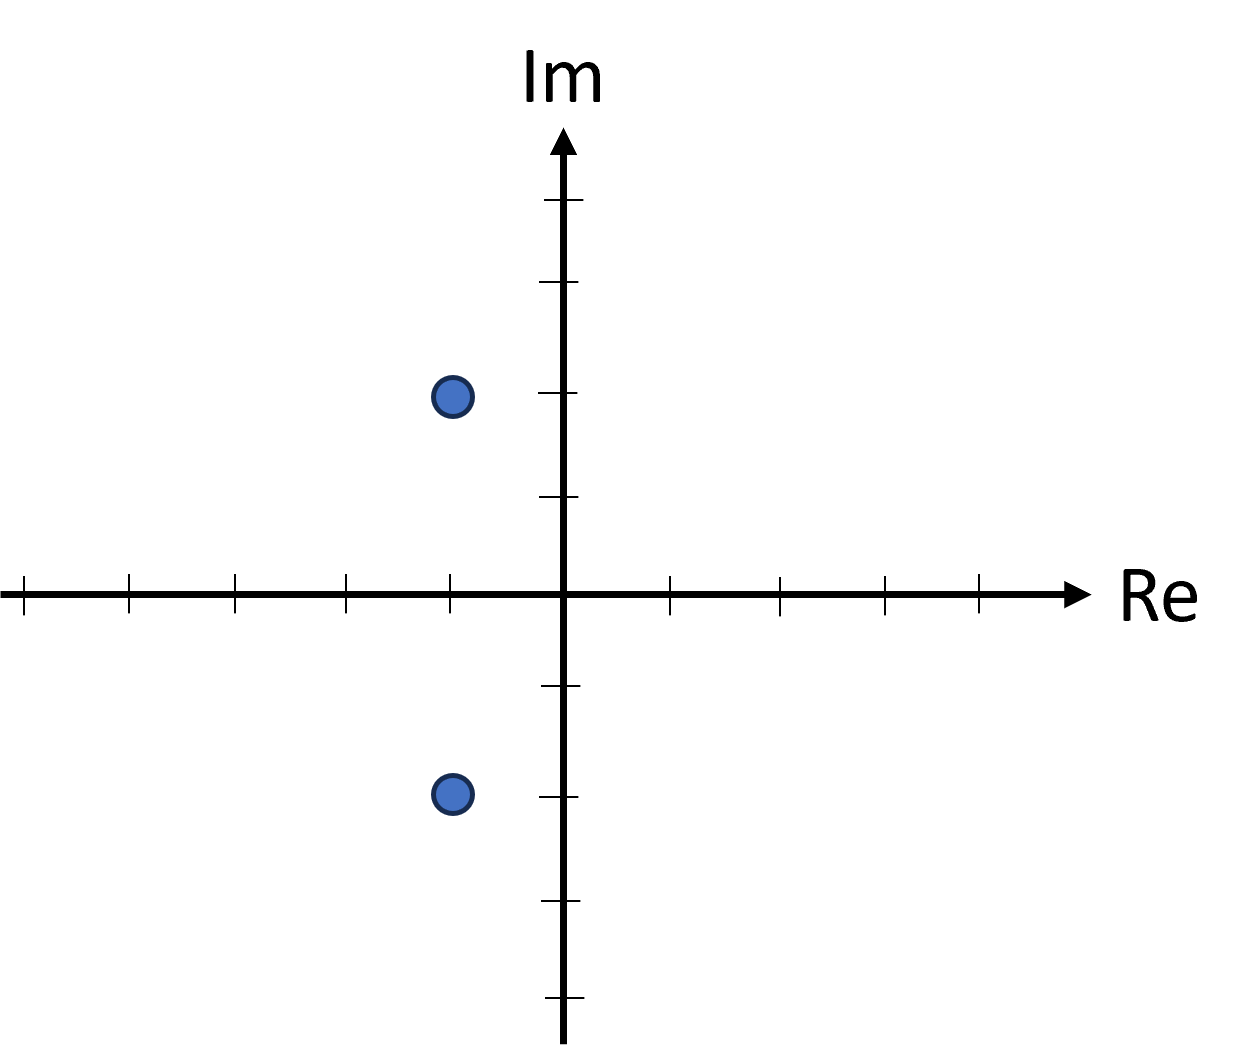
\includegraphics[width=5cm]{../Mathematik_2/Bilder/systemanalyse_konjugiert_komplexe_polstellen.png}
\end{center}

\begin{enumerate}
\item Lesen Sie die Polstellen aus der Skizze ab.
\item Geben Sie ein m�gliches Polynom an, das im Nenner der �bertragungsfunktion stehen k�nnte.
\end{enumerate}

\end{exercisebox}

 \newpage

% \appendix
% % Mathematik 2
% \setcounter{exercise}{0} \section*{Taylorreihen Aufgaben mit L�sungen}\label{MA2-taylorreihen-loesungen}

\ifintegriereaufgaben Erkl�rungen und Beispiele, die zum Verst�ndnis der L�sungswege hilfreich sind, finden Sie im Skript\wennreferenzvorhanden{MA2-taylorreihen}{ (Abschnitt \abschnittsverweis{MA2-taylorreihen})}.\fi

\begin{exercisebox}[Taylorpolynom und Restgliedabsch�tzung] %HMI I Blatt 12, Aufgabe 1
	Bestimmen Sie f�r die Funktion \(f:x\mapsto \ln\left( x\cdot e^{-2x}\right) \) das Taylorpolynom \(3.\) Grades in \(x_0=1\) und berechnen SIe damit n�herungsweise \(f(6/5)\). Geben Sie anschlie�end eine Restgliedabsch�tzung an.

\vspace{0.3cm}
\textbf{L�sung:} \newline
	Das Taylorpolynom dritten Grades lautet
	\[ T_{3,x_0}(x) = f(x_0) + f'(x_0)\cdot (x-x_0) + f''(x_0)\cdot \frac{(x-x_0)^2}{2!} + f'''(x_0)\cdot \frac{(x-x_0)^3}{3!}\,.\]
	Durch Potenzregeln l��t sich die Funktionsabbildung vereinfachen und in der Form f�llt das Ableiten wahrscheinlich leichter
	\[ f(x) = \ln\left( x\cdot e^{-2x}\right)  = \ln(x) + (-2x)\Rightarrow \begin{cases} f'(x) = x^{-1} - 2 &\Rightarrow f'(1) = -1\,,\\ f''(x) = -x^{-2} &\Rightarrow f''(1) = -1\,, \\  f'''(x) = 2x^{-3} &\Rightarrow f'''(1) = 2\,,\\ f^{(4)}(x) = -3! \,x^{-4} &\Rightarrow f^{(4)}(1) = -3! \end{cases} \]
	Das gesuchte Taylorpolynom f�r \(x_0 = 1\)
	\[ T_{3,1}(x) = -2 + (-1)\cdot (x-1) + (-1) \cdot \frac12 \cdot (x-1)^2 + 2\cdot \frac{1}{3!} (x-1)^3  = -2 -(x-1)  -\frac12 \cdot (x-1)^2 + \frac{1}{3} (x-1)^3 \,.\]
	Die Approximation an der Stelle \(x=6/5\) ist
	\[ T_{3,1}\left(\frac65\right) = -2 - \frac15 - \frac12 \frac{1}{25} + \frac13\frac{1}{125} = \frac{-1500 - 150 -15 + 2}{6\cdot 125} = -\frac{1663}{2\cdot 3\cdot 125} = -\frac{1663}{750}\,.\]
	Das Restglied nach Lagrange \(R_3\) lautet
	\[ \exists \xi \in I=(1,6/5):\quad R_3(6/5) =  f^{(4)}(\xi)\cdot \frac{(1/5)^4}{4!} \,. \]
	Da der Betrag der vierten Ableitung auf \([1,6/5]\) monoton f�llt, gilt:
\[
\left|R_3\left(\frac65\right)\right|
\leq \frac{\max_{\xi\in[1,6/5]}|f^{(4)}(\xi)|}{4!}\left(\frac15\right)^4
=\frac{6}{24}\left(\frac15\right)^4=4\cdot10^{-4}.
\]
Der exakte Fehler ist kleiner und so muss es auch sein:
		\[ \Big| f\left(\frac65\right) - T_{3,1}\left(\frac65\right) \Big| = \Big| \ln\left(\frac65\right) - 2\frac65 + \frac{1663}{750}\Big| = 3.45\cdot 10^{-4} < 4\cdot 10^{-4}\,.\]
\end{exercisebox}

\begin{exercisebox}[Taylor-Entwicklung] %Papula I, VI, Abschnitt 3, Aufgabe 5
	Geben Sie die ersten vier Glieder der Taylorreihe folgender Funktionen mit Entwicklungspunkt $x_0$ an:
\begin{eqnarray*}
	(a)\; f:x\mapsto \mathrm{cos}(x), \; x_0 = \frac{\pi}{3} \quad\quad
	(b)\; f:x\mapsto \sqrt{x}, \; x_0 = 1 \quad\quad
	(c)\; f:x\mapsto \frac{1}{x^2} - \frac{2}{x}, \; x_0 = 1
\end{eqnarray*}
\vspace{0.3cm}
\textbf{L�sung:} \newline
Diese Aufgabe entspricht Aufgabe \(5\) in Papula Band 1, Abschnitt VI.3. Die Aufgabenstellungen sind auf Seite \(520\) und detaillierte L�sungen auf Seite \(813\) zu finden.
\begin{eqnarray*}
	(a)\quad  \cos(x) &=& \frac12 - \frac{\sqrt{3}}{2}(x-\pi/3) - \frac14(x-\pi/3)^2 + \frac{\sqrt{3}}{12}(x-\pi/3)^3 + \dots \\
	(b)\quad\quad\quad \sqrt{x} &=& 1+ \frac12(x-1) - \frac18(x-1)^2 + \frac{1}{16}(x-1)^3 + \dots \\
	(c)\quad \frac{1}{x^2} - \frac{2}{x} &=& -1 + (x-1)^2 - 2(x-1)^3 + 3(x-1)^4 + \dots
\end{eqnarray*}
\end{exercisebox}

\begin{exercisebox}[Taylor-Entwicklung] %Papula I, VI, Abschnitt 3, Aufgabe 3
	Bestimmen Sie die Taylorreihe von $f:x\mapsto \displaystyle{\frac{1}{\sqrt{1-x^3}}} $ mit Entwicklungspunkt $x_0=0$ mit Hilfe des Binomischen Lehrsatzes und berechnen Sie die ersten vier Glieder explizit.
\vspace{0.3cm}
\textbf{L�sung:} \newline
Diese Aufgabe entspricht Aufgabe \(3\) in Papula Band 1, Abschnitt VI.3. Papulas Aufgabenstellung ist auf Seite \(635\) und die detaillierte L�sung auf Seite \(813\) zu finden.
Der Trick ist sich die Binomische Reihe zur Hilfe zu nehmen. Sie lautet:
\begin{eqnarray*}
	(*) \quad (1+z)^{-1/2} = 1-\frac{z}{2}+\frac{3z^2}{8} - \frac{5z^3}{16} + \dots
\end{eqnarray*}
Das gesuchte Taylorpolynom f�r \(f\) ergibt sich gerade aus \( (*)\) mit der Substitution $z=-x^3$:
\begin{eqnarray*}
	f(x) = 1 + \frac12 x^3 + \frac38 x^6 + \frac{5}{16} x^9+\dots
\end{eqnarray*}
\end{exercisebox}

\begin{exercisebox}[Taylor-Entwicklung] %Papula I, VI, Abschnitt 3, Aufgabe 2 und 10
	\begin{itemize}
		\item[(a)] Bestimmen Sie die Taylorreihe von $f:x\mapsto \displaystyle{\mathrm{cosh}(x)} $ mit Entwicklungspunkt $x_0=0$.
		\item[(b)] Untersuchen Sie mit Hilfe des Restglieds $R_{n-1}$ f�r welche Werte $x$ die Potenzreihe gegen $\mathrm{cosh}(x)$ konvergiert. Sch�tzen Sie dazu $R_{n-1}$ geeignet ab und stellen Sie fest f�r welche \(x\in\mathbb R\) gilt \(\lim\limits_{n\to\infty} R_{n-1}=0\).
		\item[(c)] L�sen Sie die Gleichung
			\[
			\mathrm{cosh}(x) = 4-x^2\]
			n�herungsweise mit Hilfe der nach der vierten Potenz abgebrochenen Potenzreihenentwicklung von $\mathrm{cosh}(x)$. Geben Sie die L�sung mit vier Nachkommastellen an.
	\end{itemize}
\vspace{0.3cm}
\textbf{L�sung:} \newline
Diese Aufgaben finden Sie in Papula Band 1, Abschnitt VI.3. ab Seite \(635\) und die detaillierten L�sungen finden Sie zum Nacharbeiten ab Seite \(813\).
\begin{itemize}
	\item[(a)] (Papula Aufg. 2 ) \quad Es gilt
		\[ \mathrm{cosh}(x) = 1 + \frac{x^2}{2!} + \frac{x^4}{4!} + \dots = \frac{e^x-e^{-x}}{2}\,,\]
			das hei�t die Taylorreihe lautet
			\[ \sum\limits_{k=0}^\infty a_k x^k, \quad a_k = \begin{cases} 1/k!, \quad &k\textnormal{ gerade}\,,\\ 0, \quad &k\textnormal{ ungerade}\,.\end{cases} \]
		\item[(b)] Es gilt \[ |R_{2n-2}(x)| = |R_{2n-1}(x)| = \Big| \frac{\mathrm{cosh}^{(2n)}(\xi)}{(2n)!} x^{2n} \Big| = |\mathrm{cosh}(\xi)|\cdot \frac{|x|^{2n}}{(2n)!}\,,\]
			mit $\xi \in (0,x)$. Also
			\[ |\mathrm{cosh}(\xi) = \Big| \frac{e^\xi + e^{-\xi}}{2} \Big| \leq \Big| \frac{e^{|\xi|} + e^{|\xi|}}{2} \Big|  \leq e^{|x|}\,,\]

			da $|\xi| < |x|$. Damit
			\[ \lim\limits_{n\to\infty}|R_{2n-2}(x)| = \lim\limits_{n\to\infty}|R_{2n-1}(x)| = \leq e^{|x|}\cdot\lim\limits_{n\to\infty} \frac{|x|^{2n}}{(2n)!} = 0 \quad (*)\]
			Damit konvergiert die Taylorreihe f�r alle $x\in\mathbb R$ gegen $\mathrm{cosh}(x)$.

			Bemerkung zu dem Grenzwert in \( (*)\): Zu jedem beliebigen, aber fixierten \(x\in \mathbb R\), l��t sich ein \(m\in \mathbb N_0\) finden, f�r das gilt  \(|x| < m\), und damit folgt f�r alle \(n\geq m\)
			\begin{eqnarray*}
				\dfrac{|x|^{2n} }{(2n)!} &=& \underbrace{ \dfrac{ |x|\cdot |x|\cdot |x|\cdot \dots \cdot |x|^m}{1\cdot 2 \cdot 3 \cdot \cdots \cdot m} }_{ \displaystyle{=M < \infty} }\cdot \dfrac{|x|}{m+1} \cdot \dfrac{|x|}{m+2} \cdot \cdots \cdot \dfrac{|x|}{2n} \\&\leq& M \underbrace{\left( \dfrac{m}{m+1} \right)^n}_{\displaystyle{ q^m, \; q< 1}} \to 0\; \textnormal{f�r} \; n\to \infty\,.
		\end{eqnarray*}
		\item[(c)] (Papula Aufg. 10) Es ist $x^4 + 36x^2 - 72 = 0 \Rightarrow x_{1,2} \approx \pm 1.3783$
	\end{itemize}
\end{exercisebox}

\begin{exercisebox}[Taylor-Entwicklung Anwendung] %Papula I, VI, Abschnitt 3, Aufgabe 12
	Berechnen Sie einen N�herungswert der folgenden Integrale. Bestimmen Sie dazu das Taylorpolynom  mit Entwicklungspunkt $x_0=0$ bis zur angegebenen Ordnung $n$ und integrieren Sie dieses. Geben Sie das Ergebnis mit $4$ Nachkommmastellen an.
	\begin{eqnarray*}
		(a)\; \int\limits_0^{1/2} \cos(\sqrt{x})\,\mathrm{d}x, \; n=3\quad\quad (b)\; \int\limits_{0}^{2/10}\frac{e^x}{x+1}\,\mathrm{d}x,\; n=3\quad\quad (c)\; \int\limits_{0}^1\frac{\sin(x)}{x}\,\mathrm{d}x, \; n=4
	\end{eqnarray*}
\vspace{0.3cm}
\textbf{L�sung:} \newline
Diese Aufgabe entspricht Aufgabe \(12\) in Papula Band 1, Abschnitt VI.3. Die Aufgabenstellung finden Sie auf Seite \(637\) und die detaillierten L�sungen ab Seite \(815\).
\vspace{0.2cm}

Kennt man Taylorreihen von Standardfunktionen, so kann man diese benutzen, um Taylorpolynome von komplizierten Funktionen ganz ohne das Berechnen von Ableitungen und Grenzwerten zu bestimmen. Hier drei Beispiele in dieser Richtung:
	\begin{itemize}
		\item[(a)] Die Taylorentwicklung der Kosinusfunktion an der Stelle \(\tilde x_0 = \sqrt{x_0} = \sqrt{0} = 0\) lautet
			\[ \tilde x = \sqrt{x}: \quad \cos(\tilde x) = 1 - \dfrac{1}{2!} \tilde x^2 + \dfrac{1}{4!} \tilde x^4 - \dfrac{1}{6!} \tilde x^6 \pm \cdots\,.
			\]
			Im Intervall \( x \in \left(0,\frac12\right)\) l��t sich der Integrand \[f: \left(0,\frac12\right) \to \mathbb R,  x \mapsto \cos\left( \sqrt{x} \right) \] durch das folgende Polynom darstellen:
			\[ \cos\left(\sqrt{x}\right) \approx  1 - \dfrac{1}{2!} \left(\sqrt{x}\right)^2 + \dfrac{1}{4!} \left( \sqrt{x}\right)^4- \dfrac{1}{6!} \left( \sqrt{x}\right)^4 = 1 - \dfrac{1}{2!} x + \dfrac{1}{4!}x^2 - \dfrac{1}{6!}x^3 \,. \]
			Und damit erhalten wir als N�herung des Integrals
			\[  \int\limits_0^{\frac12} \cos\left( \sqrt{x} \right) \,\mathrm{d} x \approx \int\limits_0^\frac12  \left( 1 - \dfrac{1}{2!} x + \dfrac{1}{4!}x^2- \dfrac{1}{6!}x^3 \right) \,\mathrm{d} x  = \Big[ x -\dfrac14 x^2 + \dfrac{1}{3\cdot 4!} x^3  - \dfrac{1}{4\cdot 6!} x^4 \Big]_0^\frac12 \approx 0,4392\,.  \]
			Das Taylorpolynom zweiter Ordnung des Integranden l��t sich formal eigentlich nicht entwickeln, denn die Ableitungen \(f^{(k)}\) f�r \( k\geq 1\) sind an der Stelle \(x_0=0\) gar nicht definiert. Die Ableitungen lassen sich f�r \(x \downarrow 0\) rechtsseitig stetig fortsetzen und betrachtet man diese Fortsetzungen, so gelangt man zu derselben polynomialen Approximation des Integranden in der N�he von \(x_0 =0\). Im aufgef�hrten L�sungsweg tritt die Problematik nicht auf, weil allein eine Entwicklung der Kosinusfunktion und die rechtsseitige Stetigkeit der Wurzelfunktion benutzt werden.
		\item[(b)]
		Die Taylorentwicklung der Exponentialfunktion an der Stelle \( x_0 = 0\) lautet
		\[ e^x =  1 + x + \frac12 x^2 + \frac{1}{3!} x^3 + \frac{1}{4!}x^4 +\cdots\,.
			\]
			Im Intervall \( x \in \left(0,\frac{2}{10}\right) \) l��t sich der Integrand \[f: \left(0,\frac{2}{10}\right) \to \mathbb R,  x \mapsto \dfrac{e^x}{x+1} \] durch das folgende Polynom darstellen:
				\begin{eqnarray*} \dfrac{e^x}{x+1} &\approx&  \dfrac{ 1 + x + \frac12 x^2 + \frac16 x^3 \frac{1}{24}x^4}{1+x} = 1 + \frac12 x^2 \dfrac{ 1 + \frac13 x + \frac{1}{12} x^2 }{1+x} \\&& = 1 + \frac12 x^2 + \frac16 x^3\dfrac{-2 + \frac14x}{1+x} = 1 + \frac12 x^2 - \frac13 x^3 + \frac{7}{48}\dfrac{x^3}{1+x}  \,. \end{eqnarray*}
			Und damit erhalten wir als N�herung des Integrals
			\[  \int\limits_0^{\frac{2}{10}} \dfrac{e^x}{1+x} \,\mathrm{d} x \approx \int\limits_0^\frac{2}{10}  \left(  1 + \frac12 x^2 - \frac13 x^3 \right) \,\mathrm{d} x  = \Big[ x +\dfrac16 x^3 - \dfrac{1}{12} x^3 \Big]_0^\frac{2}{10}  \approx 0.2012\,.  \]
			Das Taylorpolynom dritter Ordnung l��t sich auch gem�� Definition bestimmen. Die Ableitungen sind aufwendig und die vorgeschlagene L�sung ist eleganter.
		\item[(c)]
		Die Taylorentwicklung der Sinusfunktion an der Stelle \(x_0 = 0\) lautet
		\[ \sin(x) =  x - \frac{1}{3!} x^3 + \frac{1}{5!} x^5\pm\cdots\,.
			\]
			Im Intervall \( x \in (0,1) \) l��t sich der Integrand \[f: (0,1) \to \mathbb R,  x \mapsto \dfrac{\sin(x)}{x} \] durch das folgende Polynom darstellen:
				\begin{eqnarray*} \dfrac{\sin(x)}{x} &\approx&  1 - \frac{1}{3!} x^2 + \frac{1}{5!} x^4   \,. \end{eqnarray*}
			Und damit erhalten wir als N�herung des Integrals
			\[  \int\limits_0^{1} \dfrac{\sin(x)}{x} \,\mathrm{d} x \approx \int\limits_0^1  \left(  1 - \frac16 x^2 + \frac{1}{120} x^4 \right) \,\mathrm{d} x  = \Big[ x -\dfrac{1}{18} x^3 + \dfrac{1}{600} x^5 \Big]_0^1  \approx 0.9460\,.  \]
	\end{itemize}
\end{exercisebox}


\begin{exercisebox}[Taylor-Entwicklung Anwendung] %Papula I, VI, Abschnitt 3, Aufgabe 13
	Bestimmen Sie die Taylorreihe von $f: x\mapsto \ln(1-x)$ mit $x_0=0$ und differenzieren Sie diese gliedweise. Welche Potenzreihe erhalten Sie?

\vspace{0.3cm}
\textbf{L�sung:} \newline
	Diese Aufgabe entspricht Aufgabe \(13\) in Papula Band 1, Abschnitt VI.3. Die Aufgabenstellung finden Sie auf Seite \(637\) und die detaillierten L�sungen ab Seite \(817\).


\vspace{0.2cm}
Die Idee dieser Aufgabe ist zu vermitteln, dass man Taylorreihen gliedweise differenzieren kann und die Potenzreihe, die durch diese Differentiation entsteht, kann ihrerseits bzgl. Konvergenz diskutiert werden.

Die Taylorreihe der Funktion \(f: x\mapsto \ln(1-x)\) lautet:
\begin{eqnarray*} T_{f,0}(x) &=& - \sum\limits_{k=1}^\infty \dfrac1k x^k \\ \dfrac{\mathrm d}{\mathrm d x} T_{f,0}(x) &=& - \sum\limits_{k=0}^\infty x^k = - \dfrac{1}{1-x}, \quad |x|< 1 \,.\end{eqnarray*}
\end{exercisebox}

 \newpage
%
% \setcounter{exercise}{0} \section*{Integral Aufgaben mit L�sungen}\label{MA2-integration-loesungen}

\ifintegriereaufgaben Erkl�rungen und Beispiele, die zum Verst�ndis der L�sungswege hilfreich sind, finden Sie im Skript\wennreferenzvorhanden{MA2-integration}{ (Abschnitt \abschnittsverweis{MA2-integration})} des Skripts.\fi

\begin{exercisebox}[Fl�cheninhalt]
	Berechnen mit Hilfe geometrischer �berlegungen den Fl�cheninhalt zwischen Graphen und $x$-Achse

	\begin{eqnarray*}
		(a) \;  \displaystyle{ \int\limits_0^4} (2x-1) \mathrm{d}x \quad  \quad  (b) \; \displaystyle{ \int\limits_0^2} (x-1)^3 \mathrm{d}x  \quad \quad (c) \; \displaystyle{ \int\limits_0^1} |\sin(2\pi x)| \mathrm{d}x
	\end{eqnarray*}

\vspace{0.3cm}
\textbf{L�sung:} \newline
\begin{itemize}
	\item[(a)] $f: x \mapsto 2x-1, \quad f(\frac12) = 0 \Rightarrow A = -\frac12\cdot \frac12 \cdot 1 + \frac12 \cdot 7 \cdot (4-\frac12) = 12 \,. $
	\item[(b)] $\forall x \in [0,1]: \quad f(x) = -f(x+1) \Rightarrow A = 0$
	\item[(c)] $ A = \frac12 1 \cdot 1 = \frac12$
\end{itemize}
\end{exercisebox}

\begin{exercisebox}[Fl�cheninhalt (Trapezformel)] % LS p 153
	\begin{itemize}
		\item[(a)] $A$ sei der Fl�cheninhalt eines Kreises mit Radius $r$. Zeigen Sie: $ 2r^2 < A < 4 r^2$.
		\item[(b)] �berlegen Sie sich, wie Sie den Fl�chenhinhalt $A$ n�herhungsweise mit einer numerischen Integration berechnen k�nnen.
		\item[(c)] Was ist der Unterschied zur Fl�cheninhaltsberechnung von Vielecken?
	\end{itemize}

\vspace{0.3cm}
\textbf{L�sung:} \newline

\begin{itemize}
	\item[(a)] Einbeschriebenes Quadrat hat die Fl�che \( (\sqrt{2}r)^2 \) und das umschreibende Quadrat die Fl�che \( (\sqrt{4} r)^2\).
	\item[(b)] Eine Idee ist die Fl�che unter einem Halbkreis zu berechnen.  Der Halbkreis ist n�mlich als Funktion darstellbar und durch \(f: x\mapsto \sqrt{r^2-x^2}\) zu parametrisieren. Den Fl�cheninhalt kann man durch eine Zerlegungssumme approximieren, beispielsweise durch die Trapezformel. Dazu unterteilen wir das Intervall \( [-r,r]\) in \(n\in\mathbb N\) Teilintervalle mit Schrittweite $h=2r/n$ also \(x_k = -r + k\cdot h\) und berechnen sie Zerlegungssumme \(S_n\):\footnote{Sp�ter lernen wir die numerische Integration mit Zufallszahlen kennen, die sogenannte Monte-Carlo Methode}
	\[ S_n = \sum\limits_{k=0}^{n}  \frac{ f( x_{k+1}) + f(x_k)}{2} \cdot h  \Rightarrow  A \approx \lim\limits_{n\to \infty} 2\cdot S_n = \pi r^2\,.\]
\item[(c)] Anders als bei Vielecken, kann der Fl�cheninhalt nicht exakt bestimmt werden (die Kr�mmung des Funktionsgraphen ist nie konstant!). Um die Fl�chenberechnung zu berechnen muss ein Grenzwert gebildet werden.
	\end{itemize}
\end{exercisebox}
\begin{exercisebox}[Eigenschaften des Integrals]
	Begr�nden Sie, dass jede Integralfunktion $ F(x):= \displaystyle{\int\limits_{a}^x} f(t)\,\mathrm{d}t$ mindestens eine Nullstelle hat.

\vspace{0.3cm}
\textbf{L�sung:} Das ist eine Anwendung der Eigenschaften des Riemann-Integrals, denn es gilt $ \displaystyle{\int\limits_{a}^a} f(t)\,\mathrm{d}t = 0$.
\end{exercisebox}


\begin{exercisebox}[Hauptsatz der Differential- und Integralrechnung]  %Papula 1, V, Abschnitt 1-7, Aufg. 1
	Bestimmen Sie alle Stammfunktionen folgender Funktionen:
	\begin{eqnarray*}
		\begin{array}{l l l }
			(a) \;  x\mapsto 4x^5-6x^3+8x^2-3x +5
			& (b) \; x\mapsto e^x + x^2 - 2x + \sin(x)
			& (c)\; x\mapsto \displaystyle{\frac{\tan(x)}{\sin(2x)}}
		\end{array}
	\end{eqnarray*}

\vspace{0.3cm}
\textbf{L�sung:} \newline
Die hier gestellten Aufgaben (und viele mehr :) ) finden Sie in Papula, Band 1, Abschnitt V.1-7. Aufgaben ab Seite \(559\) und die L�sungen auf Seite \(787\)
\begin{itemize}
\item[(a)] Papula Aufg. 1.a) $\quad F(x) = \displaystyle{\frac23} x^6 - \displaystyle{\frac32}x^4 + \displaystyle{\frac83} x^3 - \displaystyle{\frac32} x^2 + 5x + C $
	\item[(b)] Papula Aufg. 2.a) $\quad F(x) = e^x + \displaystyle{\frac13} x^3 - x^2 - \cos(x) + C $
	\item[(c)] Papula Aufg. 2.j) $\quad F(x) = \displaystyle{\frac12}\tan(x) + C $
\end{itemize}
\end{exercisebox}

\begin{exercisebox}[Bestimmte und uneigentliche Integrale] %Papula 1, V, Abschnitt 1-7, Aufg. 3
	% https://mathematikalpha.de/wp-content/uploads/2016/05/aufg125.pdf
	Bestimmen Sie die Werte der folgenden Integrale, vorausgesetzt sie existieren:
	\begin{eqnarray*}
		\hspace{-0.3cm}
		\begin{array}{l l l l}
			(a) \; \displaystyle{\int_0^4} \left( x^3 - 5x^2 + \frac32 x -10\right)\, \mathrm{d}x & (b)\; \displaystyle{\int_1^4} \displaystyle{\frac{1-z^2}{z}}\,\mathrm{d}z &(c)\; \displaystyle{\int_0^{0,5}} \displaystyle{\frac{3}{\sqrt{1-x^2}}}\, \mathrm{d}x & (d)\; \displaystyle{\int_0^{\pi/4}} \displaystyle{\frac{1-\cos^2(x)}{2\cos^2(x)}}\,\mathrm{d}x \\[2ex]
			(e) \; \displaystyle{\int_1^\infty} \frac{1}{x^4}\,\mathrm{d} x & (f)\; \displaystyle{\int_0^\infty} \displaystyle{\frac{1}{x}}\,\mathrm{d}x  & (g)\; \int\limits_{-\infty}^0 e^{-t}\,\mathrm{d}t &(h)\; \displaystyle{\int_0^{4}} \displaystyle{\frac{2}{\sqrt{t}}}\, \mathrm{d}t
		\end{array}
	\end{eqnarray*}

\vspace{0.3cm}
\textbf{L�sung:} \newline
Die hier gestellten Aufgabenteile \( (a)- (d) \) finden Sie in Papula, Band 1, V.1-7, ab Seite \(560\) und die L�sungen auf Seite \(787\)
\begin{itemize}
	\item[(a)] Papula Aufg. 3.a) $\quad -212/3 $
	\item[(b)] Papula Aufg. 3.c) $\quad \ln(4) - 15/2 $
	\item[(c)] Papula Aufg. 3.i) $\quad \pi/2 $
	\item[(d)] Papula Aufg. 3.j) $\quad (1-\pi/4)/2 $
	\item[(e)]
	\[ \int\limits_1^a \frac{1}{x^4}\,\mathrm{d}x = \Big[ -\frac{1}{3x^3}\Big]_1^a = -\frac{1}{3a^3} + \frac13 \Rightarrow \lim\limits_{a\to\infty} \left( -\frac{1}{3a^3} + \frac13\right) = \frac13\,. \]
	\item[(f)]
		\[ \int \frac{1}{x}\,\mathrm{d}x = \ln(x)+C \Rightarrow \lim\limits_{a \to 0}\int\limits_{a}^{1} \frac1x\,\mathrm{d}x + \lim\limits_{b\to\infty} \int\limits_{1}^{b} \frac1x\,\mathrm{d}x\]
Keines der beiden uneigentlichen Integrale existiert: $\lim\limits_{a\to 0} \ln(a) = -\infty$ und  $\lim\limits_{b\to\infty} \ln(b) = \infty$
	\item[(g)]
		\[ \int\limits_a^0 e^{-t}\,\mathrm{d}t = \Big[ - e^{-t}\Big]_a^0 = -1 + e^{-a} \Rightarrow \lim\limits_{a\to-\infty} \left( -1 + e^{-a}\right) = \lim\limits_{a\to \infty} \left( -1 + e^a\right)  \textnormal{ existiert nicht}\,. \]
	\item[(h)]
\[ \int\limits_a^4 \frac{2}{\sqrt{t}}\,\mathrm{d}t = \Big[ 4 \sqrt{t}\Big]_a^4 = 8 - 4\sqrt{a} \Rightarrow \lim\limits_{a\to 0} \left( 8 - 4\sqrt{a}\right) = 8\,. \]
\end{itemize}
\end{exercisebox}

\begin{exercisebox}[Numerische Integration]
	Das folgende bestimmte Integral soll n�herungsweise bestimmt werden:
	\[
		\int_1^3 x^3 \, \mathrm{d}x = 20\,.
	\]
	\begin{itemize}
		\item[(a)] Bestimmen Sie eine Zerlegung des Intervalls $[1,3]$ in $4$ gleich gro�e Intervalle.
		\item[(b)] Wenden Sie eine Rechteckregel an.
		\item[(c)] Wenden Sie die Trapezregel an.
		\item[(d)] Wenden Sie die Simpson-Formel an.
	\end{itemize}
\vspace{0.3cm}
\textbf{L�sung:}
\begin{itemize}
	\item[(a)] $x_0=1, x_1 = \frac32, x_2 = 2, x_3=\frac52, x_4=3$
	\item[(b)] $A = \frac12\cdot (1^3 + (\frac32)^3 + 2^3 + (\frac52)^3) = 14$
	\item[(c)] $A = \frac14\cdot 1^3 + \frac12( (\frac32)^3 + 2^3)  + \frac14 (\frac52)^3) = 20.5$
\item[(d)] Zur Anwendung der Simpson-Formel brauchen wir noch alle Zwischenstellen: \[ x_{0}=0, x_{01}=\frac54, x_1 = \frac32, x_{12}=\frac74, x_2 = 2, x_{23}=\frac94, x_3=\frac52, x_{34} = \frac{11}{4}, x_4=3\,.\]
	Die Simpson-Formel ergibt: \begin{eqnarray*} A&=&\frac{1}{12} \left( 1^3 + 4 \left( \frac54\right)^3 + 2 \left( \frac32\right)^3 + 4 \left( \frac74\right)^3 + 2 \left( 2\right)^3 + 4  \left( \frac94\right)^3 + 2 \left( \frac52\right)^3 + 4  \left( \frac{11}{4}\right)^3 + 3^3\right) \\
	&=& \cdots = 20\,.\end{eqnarray*}
	Das Ergebnis h�tten wir auch ohne Rechnung sofort angeben k�nnen, denn die Simpson-Formel ist exakt f�r Polynome dritten Grades. Dieses Ergebnis l��t sich sofort der Fehler-Absch�tzung ablesen - warum?
\end{itemize}
\end{exercisebox}

\begin{exercisebox}[Simpson-Regel]
	Bestimmen Sie den relativen Fehler, den Sie bei einer Approximation des Intgrals \[ I = \int\limits_0^1 f(x) \, \mathrm d x = \int\limits_0^1 x\cdot \cos(x^2) \, \mathrm d x\] mit Hilfe der Simpson-Regel auf drei �quidistanten Teilintervallen machen.

\vspace{0.3cm}
\textbf{L�sung:}
Auszuwerten ist die Simpsonregel f�r \(h=\dfrac13\). Zus�tzlich zu den St�tzpunkten in Intervallr�ndern kommen St�tzpunkte in jeder Intervallmitte. Insgesamt sind das also \(7\) St�tzpunkte \[ \begin{cases} x_k &= 0+ k\cdot \dfrac12 h = k\cdot \dfrac16 \,, \\ y_k &= f(x_k) = x_k \cdot \cos\left( x_k^2\right) \,. \end{cases} \] Mit dieser Notation lautet die Simpsonregel also
\[ S_3(f) = h\left( \dfrac{1}{6} y_0 +  \dfrac23 y_1 + \dfrac13 y_2 + \dfrac23 y_3 + \dfrac13 y_4 + \dfrac23 y_5 + \dfrac16 y_6 \right) = \sum\limits_{k=0}^6 w_k y_k, \]
\small{
\begin{tabular}{c | c c c c c c c}
\(k\) & \(0\) & \(1\) & \(2\) & \(3\) & \(4\) & \(5\) & \(6\) \\\hline
\(x_k\) & \(0\) & \(\dfrac16\) & \(\dfrac26\) & \(\dfrac36\) & \(\dfrac46\) & \(\dfrac56\) & \(\dfrac66\) \\[2ex]
\(y_k\) & \(\dfrac16\cos\left(\dfrac{1}{36}\right)\) & \(\dfrac13\cos\left(\dfrac{1}{9}\right)\) & \(\dfrac12\cos\left(\dfrac14\right)\) & \(\dfrac23\cos\left( \dfrac49\right)\) & \(\dfrac23\cos\left( \dfrac49\right)\) & \(\dfrac56\cos\left(\dfrac{25}{36}\right)\) & \(\cos\left(1\right)\) \\[2ex]
\(w_k\) & \(\dfrac13 \cdot \dfrac16\) & \(\dfrac13 \cdot \dfrac23\)& \(\dfrac13 \cdot \dfrac13\) & \(\dfrac13 \cdot \dfrac23\) & \(\dfrac13 \cdot \dfrac13\) & \(\dfrac13 \cdot \dfrac23\)  & \(\dfrac13 \cdot \dfrac16\)
\end{tabular}
}

Damit \[ S_{3}(f) = \sum\limits_{k=0}^6 w_k \cdot y_k = 0.420681 \,.\]
Analytische Integration liefert \[ I = \int\limits_0^1 x\cdot \cos(x^2)\,\mathrm{d}x = \Big[ \dfrac12 \sin(x^2)\Big]_0^1 = 0.420736\,.\]
Damit ergibt sich f�r den relativen Fehler:
\[e= \dfrac{ | I - S_{3} |}{ I} = 1.31\cdot 10^{-4}\,.\]
\end{exercisebox}

 \newpage
% \setcounter{exercise}{0} \section*{Integrationsregeln Aufgaben mit L�sungen}\label{MA2-integrationsregeln-loesungen}

\ifintegriereaufgaben Erkl�rungen und Beispiele, die zum Verst�ndis der L�sungswege hilfreich sind, finden Sie im Skript\wennreferenzvorhanden{MA2-integrationsregeln}{ (Abschnitt \abschnittsverweis{MA2-integrationsregeln})}. \fi

\begin{exercisebox}[St�ckweise stetige Funktionen] %A.Z. Erweiterungen
	Gegeben seien die folgenden st�ckweise definierten Funktionen
	\begin{eqnarray*}
		f:x\mapsto \begin{cases} x, \quad &x<1\,,\\ x-1, \quad &x\geq 1 \end{cases}\quad \quad g:x\mapsto \begin{cases} x, \quad & x<1\,,\\ 2, \quad & x=1\,,\\ \cos(x),\quad & x>1 \end{cases}
	\end{eqnarray*}
			\begin{itemize}
				\item[(a)] Integrieren Sie diese Funktionen st�ckweise.
				\item[(b)] Sind die Funktionen, die Sie unter \( (a)\) entwickelt haben Stammfunktionen?
			\end{itemize}


\vspace{0.3cm}
\textbf{L�sung:} \newline
\begin{itemize}
	\item[(a)] Wir integrieren st�ckweise und erhalten
\begin{eqnarray*}
	F(x) &=& \begin{cases} \displaystyle{\int} x \,\mathrm{d}x = \frac12 x^2+ c_1, \quad & x< 1\,,\\ \displaystyle{\int} x-1 \,\mathrm{d}x = \frac12 x^2 - x +c_2, \quad & x > 1 \end{cases} \\[1ex]
	G(x) &=& \begin{cases} \displaystyle{\int} x\,\mathrm{d}x = \frac12 x^2+c_1, \quad & x< 1\,,\\[1ex] \displaystyle{\int} \cos(x) \,\mathrm{d}x = \sin(x) +c_2,\quad & x> 1\end{cases}
\end{eqnarray*}

\item[(b)] Achtung! Die Funktionen \(F\) und \(G\), die unter \( (a)\) durch eine st�ckweise Integration ermittelt worden sind, sind keine Stammfunktionen - denn sie sind nicht stetig geschweige denn differenzierbar.
\end{itemize}
Bemerkung: man kann f�r diesen Fall sogenannte verallgemeinerte Stammfunktionen definieren, aber diese ben�tigen wir nicht.
%Sie lauten
%\begin{eqnarray*}
%	\tilde F(x) &=& \begin{cases}\frac12 x^2+ c, \quad & x< 1\,,\\ (x-1)^2 +c, \quad & x\geq 1 \end{cases} \\
%	\tilde G(x) &=& \begin{cases} x^2+c, \quad & x< 1\,,\\ \sin(x) - \sin(1) +1 +c,\quad & x\geq 1\end{cases}
%\end{eqnarray*}

\end{exercisebox}

\begin{exercisebox}[Partielle Integration] % Papula 1, V, Abschnitt 8, Aufgabe /6
	Berechnen Sie die folgenden Integrale:
	\begin{eqnarray*}
		(a)\; \int x \ln(x) \, \mathrm{d}x \quad
		(b)\; \int_1^5 \ln(t) \, \mathrm{d}t \quad
		(c)\; \int_0^{0,8} x e^x \, \mathrm{d}x\quad
		(d)\; \int e^x \cos(x) \, \mathrm{d}x
	\end{eqnarray*}
	Finden Sie eine Rekursionsformel zur Berechnung von \[ \int x^n\cdot e^x \, \mathrm d x, \quad n\in \mathbb N^+\,.\]

\vspace{0.3cm}
\textbf{L�sung:} \newline
Diese Aufgaben finden Sie in Papula, Band 1, Abschnitt V.\(8\) auf Seite \(562\) und detaillierte L�sungswege auf Seite \(792\)ff.
\begin{itemize}
	\item[(a)] Papula Aufg. 5.a) $\quad  \frac14 x^2(2\ln(x) -1)+C $
\item[(b)] Den Logarithmus kann man integrieren mit Hilfe einer partiellen Integration. W�hle
	\[\begin{cases} \ln(t) & \stackrel{\frac{\mathrm d }{\mathrm d t}}{\rightarrow} \dfrac{1}{t}\\
					1 & \stackrel{\int \cdot \mathrm d t}{\rightarrow} t
				\end{cases}\; \Rightarrow \;
			\int 1 \cdot \ln(t) \,\mathrm d t = \ln(t)\cdot t - t + c \; \Rightarrow \; \int\limits_1^5 \ln(t) \, \mathrm{d}t = 5\ln(5)-4\,.\]
	\item[(c)] Papula Aufg. 5.e) $\quad  -0,2 \cdot e^{0,8} + 1 $
	\item[(d)] Papula Aufg. 6.a) $\quad  \frac12 e^x( \sin(x) + \cos(x)) +C $
\end{itemize}
Zur Rekursionsformel:
\[ \begin{array}{rcl} I_0 &=& \displaystyle \int e^x \, \mathrm{d}x = e^x \\ n\geq 1:\quad  I_n  &=& \displaystyle \int x^n\cdot e^x\, \mathrm d x\,, \quad \mbox{P.I. mit }\left\{ \begin{array}{r rcl} \dfrac{\mathrm d \; \cdot}{\mathrm d x} &  x^n &\longrightarrow& n\, x^{n-1} \\ \int \; \cdot \; \mathrm{d} x & e^x &\longrightarrow& e^x \end{array}\right. \\
&=& x^n\cdot e^x - \displaystyle \int n\, x^{n-1}\cdot e^x \, \mathrm d x\\ &=& x^n\cdot e^x - n \cdot \color{blue}{ \displaystyle \int x^{n-1}\cdot e^x \, \mathrm d x } =  x^n\cdot e^x - n\cdot \color{blue}{ I_{n-1}  }\,. \end{array}\]
\end{exercisebox}

\begin{exercisebox}[Integrationsregeln] % Papula 1, V Abschnitt 8, Aufg. 1
	Berechnen Sie die folgenden Integrale:
	\begin{eqnarray*}
		(a)\; \int x \sin(x^2) \, \mathrm{d}x \quad
		(b)\; \int_{-1}^{1} \frac{t}{\sqrt{1+t^2}}\, \mathrm{d}t \quad
			(c)\; \int_{-1}^{1} \frac{5+x}{5-x} \, \mathrm{d}x\quad
			(d)\; \int \frac{\sqrt{4-x^2}}{x^2} \, \mathrm{d}x
		\end{eqnarray*}

\vspace{0.3cm}
\textbf{L�sung:} \newline
Diese Aufgaben finden Sie in Papula, Band 1, Abschnitt V.\(8\) auf Seite \(562\) und detaillierte L�sungswege auf Seite \(790\)ff.
\begin{itemize}
	\item[(a)] F�hren wir eine Intgration durch Substitution durch: \(u=x^2 \; \Rightarrow \; \mathrm{d}u = 2x\mathrm{d}x\)
		\[ \int x\cdot \sin(x^2)\, \mathrm{d}x = \dfrac12 \int \sin(x^2) \cdot 2\cdot x \, \mathrm{d}x = \dfrac12 \int \sin(u)\,\mathrm{d}u = - \dfrac12 \cos(u) = -\frac12\cos(x^2)+c \,.\]
	\item[(b)] Der Integrand enth�lt einen Bruch, und es ist wichtig m�gliche Polstellen im Integrationsgebiet zu identifizieren bevor wir integrieren. Da der Nenner f�r alle \(t\in \mathbb R\) gr��er null ist, liegt hier kein Pol vor und wir k�nnen loslegen. Die Substitution \(u=1+t^2\) f�hrt auf das Differential \( \mathrm{d}u = 2t\,\mathrm{d}t\) und die neuen Integrationsgrenzen \(u(-1) = u(1) = 2\):
		\[ \int_{-1}^{1} \frac{t}{\sqrt{1+t^2}} \mathrm{d}t = \dfrac12 \int_{-1}^{1} \frac{1}{\sqrt{1+t^2}} \cdot 2\,t\, \mathrm{d}t= \dfrac12 \int_{2}^{2} \frac{1}{\sqrt{u}} \,\mathrm{d}u = 0 \,.\]
	\item[(c)] Der Integrand ist eine gebrochenrationale Funktion, die noch nicht vollst�ndig gek�rzt ist. Die Polynomdivision zerlegt den Integranden in seinen granzrationalen und echtgebrochenrationalen Anteil:
		\[ (x+5):(-x+5) = -1 + \dfrac{10}{5-x}\,.\]
		Und damit
		\[\int_{-1}^{1} \frac{5+x}{5-x} \, \mathrm{d}x = \int_{-1}^{1} \left( -1 + \dfrac{10}{5-x}\right) \, \mathrm{d}x = \Big[ -x +10 \cdot \ln|5-x|\cdot\textcolor{blue}{(-1)} \Big]_{-1}^1\int_{-1}^{1} =  10\cdot \ln(3/2) - 2 \,.\] Die blau hervorgehobene \(\textcolor{blue}{-1}\) darf nicht fehlen: sie gleicht die innere Ableitung des Arguments im Logarithmus aus!

		Ein Integral l��t sich unter Umst�nden auf viele verschiedene Arten l�sen. Im vorliegenden Fall f�hrt auch die Formel der partiellen Integration zum Erfolg: f�r \(x \in [-1,1]\) gilt
		\[\begin{cases} (5+x) & \stackrel{\frac{\mathrm d }{\mathrm d x}}{\rightarrow} +1\\
					\dfrac{1}{5-x} & \stackrel{\int \cdot \mathrm d x}{\rightarrow} -\ln(5-x) \quad \textnormal{da}\; (5-x) > 0 \,.
				\end{cases}
			\]
		Mit Aufgabe 2.b folgt
		\[ \int_{-1}^1 \ln(5-x)\,\mathrm{d} x = \Big[\left( \ln(5-x)\cdot (5-x) - (5-x) \right) (-1)\Big]_{-1}^1 = -4\ln(4) + 6\ln(6) - 2\,.\]
Also
		\begin{eqnarray*}
			\int\limits_{-1}^1 \dfrac{5+x}{5-x} \, \mathrm{d}x &=& \Big[ -\ln(5-x)\Big]_{-1}^1 + \int\limits_{-1}^1 \ln(5-x)\,\mathrm{d} x \\
		&=&  -\ln(4) + \ln(6) -4\ln(4) + 6\ln(6) - 2 = 10(\ln(3)-\ln(2))-2\,.\end{eqnarray*}


	\item[(d)] Bei Wurzelausdr�cken der Form \( \sqrt{a^2-x^2}\) ist es klug sich an die Kreisgleichung zu erinnern: \[ x^2 + y^2 = a^2 \; \Rightarrow \; \begin{cases} x &= a\cos(\alpha)\,, \\ y &=a \sin(\alpha) \end{cases} \] Sieht man diesen Zusammenhang, dann liegt die folgende Substitution nah:
		\[ x=2\cos(\alpha) \; \Rightarrow \; \mathrm{d}x = -2\sin(\alpha) \,\mathrm{d}\alpha \]
		Das Differential wird einen weiteren Faktor im Integranden erzeugen und das mag auf den ersten Blick ein no-go sein, aber auf den zweiten Blick ist es ein Gl�cksgriff, denn
	\[ \int \dfrac{\sqrt{4-x^2}}{x^2} \, \mathrm{d}x = \int \dfrac{\sqrt{4\sin^2(\alpha)}}{4 \cdot \cos^2(\alpha)} \, (-2\cdot \sin(\alpha))\,\mathrm{d}\alpha = \textcolor{blue}{\int \dfrac{\sin(\alpha)}{\cos^2(\alpha)} \, (-\sin(\alpha))\,\mathrm{d}\alpha} = - \int \tan^2(\alpha))\,\mathrm{d}\alpha \,.\]
	Und nun? Wir haben das Integral jetzt transformiert auf ein neues Integral - wie l�sen wir es? Anstatt den Integranden als \(\tan^2(\alpha)\) zu identifizieren, m�chte ich hier eine partielle Integration zur Integration des blau leuchtenden Integrals zeigen. Die Idee zur Wahl von \(f'\) und \(g\) resultiert aus
	\[ \left( \dfrac{1}{\cos(\alpha)}\right)' = -\dfrac{1}{\cos^2(\alpha)}\cdot \left(-\sin(\alpha)\right) \Rightarrow \; \int -\dfrac{1}{\cos^2(\alpha)}\cdot \left(-\sin(\alpha)\right) \, \mathrm{d}x = \dfrac{1}{\cos(\alpha)} + c\,.\]
	Also
	\[\begin{array}{rcl} \textcolor{blue}{\displaystyle{ \int \underbrace{ \dfrac{\sin(\alpha)}{\cos^2(\alpha)}}_{=:f'}} \, \underbrace{(-\sin(\alpha))}_{=:g}\,\mathrm{d}\alpha} &=&  - \sin(\alpha)\cdot \dfrac{1}{\cos(\alpha)} + \displaystyle{\int} \left(-\cos(\alpha)\right)\cdot \dfrac{1}{\cos(\alpha)} \,\mathrm{d}\alpha \\ &=& - \dfrac{\sin(\alpha)}{\cos(\alpha)} + \alpha + c \end{array}\,.\]
	Um die gesuchte Stammfunktion in Termen von \(x\) anzugeben, muss r�cksubstituiert \(x = \arccos(x)\).
	\[\int \dfrac{\sqrt{4-x^2}}{x^2} \, \mathrm{d}x = - \tan\left( \arccos(x)\right) + \arccos(x) +c \,.\]
		%$\quad  -\frac{\sqrt{4-x^2}}{x} - \arcsin(x/2)+C $
	Formal l��t sich die R�cksubstitution nat�rlich leicht durchf�hren, aber bei bestimmten Integralen muss man an der Stelle immer aufpassen. Die Arkusfunktionen kehren die trigonometrischen Funktionen nur in eingeschr�nkten Intervallen um!
\end{itemize}
\end{exercisebox}

\begin{exercisebox}[Integrationsregeln] % Papula 1, V Abschnitt 8, Aufg. 10
	Berechnen Sie die folgenden Integrale:
	\begin{eqnarray*}
		\begin{array}{rl rl rl}
			(a)\; &\displaystyle{\int} \mathrm{cot}(x) \, \mathrm{d}x \quad
			& (b)\;&\displaystyle{\int} x\mathrm{cosh}(x) \, \mathrm{d}x \quad & (c) \; & \displaystyle{\int} \displaystyle{\frac{(\ln(x))^3}{x}}\,\mathrm{d}x \\
			(d)\;& \displaystyle{\int} \displaystyle{\frac{12 x^2}{2x^3-1}} \, \mathrm{d}x  &(e)\; &\displaystyle{\int} \sqrt{x^2 - 2x} \, \mathrm{d}x \quad & (f)\;&\displaystyle{\int} \mathrm{arctan}(x) \, \mathrm{d}x
		\end{array}
	\end{eqnarray*}
\vspace{0.3cm}
\textbf{L�sung:} \newline
Diese Aufgaben finden Sie in Papula, Band 1, Abschnitt V.\(8\) auf Seite \(563\) und detaillierte L�sungswege auf Seite \(795\)ff.
\begin{itemize}
	\item[(a)] Papula Aufg. 10.b) $\quad F(x) = \ln| \sin(x)| + C  $
\item[(b)] Papula Aufg. 10.c) $\quad F(x) = x\,\mathrm{sinh}(x) - \mathrm{cosh}(x) + C $
	\item[(c)] Papula Aufg. 10.g) $\quad F(x) = \frac14(\ln(x))^4 + C $
	\item[(d)] Papula Aufg. 10.h) $\quad F(x) = 2\ln| 2x^3 - 1| + C $
\item[(e)] Papula Aufg. 10.j) $\quad F(x) = \frac12(x-1) \cdot \sqrt{x^2 - 2x} - \frac12 \,\mathrm{arcosh}(x-1) + C $
	\item[(f)] Papula Aufg. 10.l) $\quad F(x) = x\cdot \arctan(x) - \frac12 \ln(1+x^2) + C $
\end{itemize}
\end{exercisebox}

\begin{exercisebox}[Integrationsregeln]
	Berechnen Sie die folgenden Integrale:
	\begin{eqnarray*}
		\begin{array}{rl rl}
			(a)\; &\displaystyle{\int_{1/2}^1} \displaystyle{\frac{\sqrt{\frac1x + 1}}{x^2}} \, \mathrm{d}x, \quad y=\displaystyle{\frac1x} +1
			& (b)\;&\displaystyle{\int_0^{1/b}} \displaystyle{\frac{ax}{bx+c}} \, \mathrm{d}x,  \quad b\not=0, c>0, x = \displaystyle{\frac{t-c}{b}} \\
				(c) \; & \displaystyle{\int} \displaystyle{\frac{1}{\sqrt{x^2-4}}}\,\mathrm{d}x &(d)\;& \displaystyle{\int} \displaystyle{\sqrt{18 + 2x^2}} \, \mathrm{d}x
		\end{array}
	\end{eqnarray*}
\vspace{0.3cm}
\textbf{L�sung:} \newline
\begin{itemize}
	\item[(a)]
		\begin{eqnarray*}
			\int\frac{\sqrt{\frac1x + 1}}{x^2}\,\mathrm{d}x &=& -\int\sqrt{y} \, \mathrm{d}y = -\frac23y^{3/2} + c = - \frac23\left( \frac1x + 1\right)^{3/2} + c  \\
		\Rightarrow \; \int\limits_{1/2}^1\frac{\sqrt{\frac1x + 1}}{x^2}\,\mathrm{d}x &=& \Big[ -\frac23 \left( \frac1x + 1\right)^{3/2}\Big]_{1/2}^1 = 2\sqrt{3} - \frac{4\sqrt{2}}{3}
	\end{eqnarray*}
	Alternativ - direkt durch Transformation der Grenzen:
		\begin{eqnarray*}
		\int\limits_{1/2}^1\frac{\sqrt{\frac1x + 1}}{x^2}\,\mathrm{d}x =  - \int\limits_{2}^3\sqrt{y}\,\mathrm{d}y =  \Big[ -\frac23 y^{3/2}\Big]_{2}^3 = 2\sqrt{3} - \frac{4\sqrt{2}}{3}
	\end{eqnarray*}
	\item[(b)]
		\begin{eqnarray*}
			\int\displaystyle{\frac{ax}{bx+c}} \, \mathrm{d}x &=& \int \frac{a \frac{t-c}{b}}{b\frac{t-c}{b} + c } \cdot \frac1b \,\mathrm{d}x  = \frac{a}{b^2} \int \frac{t-c}{t}\,\mathrm{d}t = \frac{a}{b^2} \int (1-\frac{c}{t})\,\mathrm{d}t \\
				&=&  \frac{a}{b^2}\cdot ( t-c\ln(|t|) +C \frac{a}{b} x -\frac{ac}{b^2} \ln|bx+c| +C \\
					\Rightarrow \int \displaystyle{\frac{ax}{bx+c}} \, \mathrm{d}x &=& \Big[ \frac{a}{b} x - \frac{ac}{b^2} \ln|bx+c| +C \Big]_0^{1/b} =\frac{a}{b^2} \left( 1-c\ln\frac{c}{1+c}\right)
					\end{eqnarray*}
	Alternativ - direkt durch Transformation der Grenzen:
	\begin{eqnarray*}
		\int\limits_0^{1/b} \displaystyle{\frac{ax}{bx+c}} \, \mathrm{d}x = \int_{c}^{1+c} \frac{a\frac{1-c}{b}}{b\frac{t-c}{b} + b}\cdot \frac{1}{b} \,\mathrm{d}t = \Big[ \frac{a}{b^2}\left( t-c\ln|t|\right) \Big]_c^{1+c} =\frac{a}{b^2} \left( 1-c\cdot \ln\frac{c}{1+c}\right)
		\end{eqnarray*}

	\item[(c)]
		\begin{eqnarray*}
			\int\frac{1}{\sqrt{x^2-4}}\,\mathrm{d}x &=&  \int\frac{1}{\sqrt{4\mathrm{cosh}^2(t)-4}}\cdot 2 \cdot \mathrm{sinh}(t)\,\mathrm{d}t = \int \frac{1}{\mathrm{sinh}(t)}\mathrm{sinh}(t)\,\mathrm{d}t \\
			&=& t+c = \mathrm{arcosh}(x/2)+c
		\end{eqnarray*}
	\item[(d)]
		\begin{eqnarray*}
			\int\sqrt{18 + 2x^2}\,\mathrm{d}x &=&
			\frac{1}{\sqrt{2}} \int \sqrt{9+x^2}\,\mathrm{d}x = \frac{1}{\sqrt{2}} \int \sqrt{9+9\,\mathrm{sinh}^2(t)} \cdot 3\, \mathrm{cosh}(t) \, \mathrm{d}t \\
			&=& \frac{1}{\sqrt{2}} \int\mathrm{cosh}(t) \cdot \mathrm{cosh}(t)\,\mathrm{d}t \\
			\Rightarrow \int\mathrm{cosh}^2(t)\,\mathrm{d}t &=& \frac14\int\left( e^{2t} + 2 + e^{-2t}\right) \, \mathrm{d}t = \frac{\mathrm{sinh}(2t)}{4} + \frac12 t + c = \frac12(\mathrm{cosh}(t) \mathrm{sinh}(t) + t ) + c \\
			\Rightarrow  \int\sqrt{18 + 2x^2}\,\mathrm{d}x &=& \frac{1}{2\sqrt{2}}\left( \mathrm{cosh}\left( \mathrm{arsinh}(x/2)\right)/2 - \mathrm{arsinh}(x/2)\right) + c
		\end{eqnarray*}
\end{itemize}
\end{exercisebox}

%\begin{exercisebox}[Gebrochenrationale Funktionen]
%	Berechnen Sie folgende Integrale. Hinweis: Nutzen Sie die Ergebnsise auf Blatt $1$.
%	\begin{eqnarray*}
%		\begin{array}{l l l}
%			(a)\; \displaystyle{ \int \frac{-x^4-2x^3+7x^2-5x+3}{ x^2+3x-4}} \, \mathrm{d}x \quad & (b)\; \displaystyle{\int \frac{x^2+x+1}{x^3-3x+2}}\,\mathrm{d}x  & (c) \; \displaystyle{\int \frac{1}{x^3+x}}\,\mathrm{d}x \\[1ex]
%			(d)\; \displaystyle{\int \frac{x^2-5x}{(x-2)^3}} \,\mathrm{d}x &(e)\; \displaystyle{ \int \frac{1}{ x^2-a^2}} \, \mathrm{d}x, \; a>0 & (f)\; \displaystyle{\int \frac{4x^3}{x^3+2x^2-x-2}}\,\mathrm{d}x \\[2ex]
%			(g) \; \displaystyle{\int \frac{3z}{z^3-3z^2-4}}\,\mathrm{d}x  & (h)\; \displaystyle{\int \frac{4x-2}{x^2-2x-63}}\, \mathrm{d}x \quad & (i)\; \displaystyle{\int \frac{2x+1}{x^3-6x^2+9x}}  \, \mathrm{d}x
%		\end{array}
%	\end{eqnarray*}
%\vspace{0.3cm}
%\textbf{L�sung:} \newline
%Detaillierte L�sungen zu den Aufgabenteilen \((e) -(i)\) finden Sie in Papula, Band \(1\) auf Seite \(793\)ff.
%\begin{itemize}
%	\item[(a)] $ F(x) = - \displaystyle{\frac{7}{5}}\ln|x+4| - \displaystyle{\frac{x^3}{3}} + \displaystyle{\frac{x^2}{2}}  + \displaystyle{\frac{2}{5}} \ln|x-1| + c $
%	\item[(b)] $ F(x) = \displaystyle{\frac{1}{3}} \ln|x+2| - \displaystyle{\frac{1}{x-1}} + \displaystyle{\frac{2}{3}}\ln|x-1| + c $
%	\item[(c)] $ F(x) = -\displaystyle{\frac{1}{2}} \ln(x^2+2) + \ln|x| + c $
%	\item[(d)] $ F(x) = \displaystyle{\frac{1}{x-2}} + \displaystyle{\frac{3}{(x-2)^2}} + \ln|x-2| c $
%	\item[(e)] $ F(x) = \displaystyle{\frac{1}{2a}} \ln\Big| \displaystyle{\frac{x-a}{x+a}}\Big| + c $
%	\item[(f)] $ F(x) = \displaystyle{\frac{2}{3}} \ln| x-1| + 2 \ln|x+1| - \displaystyle{\frac{32}{3}}\ln|x+2| + 4x + c $
%	\item[(g)] $ F(x) = \displaystyle{\frac{1}{3}} \ln\Big| \displaystyle{\frac{z-1}{z+2}}\Big| - 2 \displaystyle{\frac{2}{z+2}} + c $
%	\item[(h)] $ F(x) = \displaystyle{\frac{17}{8}} \ln|x-9| + \displaystyle{\frac{15}{8}}\ln|x+7| + c $
%	\item[(i)] $ F(x) = \displaystyle{\frac{1}{9}} \ln\Big| \displaystyle{\frac{x}{x-3}}\Big| - \displaystyle{\frac{7}{3(x-3)}} + c $
%\end{itemize}
%\end{exercisebox}

\begin{exercisebox}{Kurvendiskussion mit Fl�chenberechnung}{ } %p. 176
		Gegeben ist die Funktion \(f\) mit \(f:x\mapsto x^2(x^2-4)\). Ihr Graph sei \(K\).
		\begin{itemize}
			\item[(a)] Untersuchen Sie \(f\) und zeichenn Sie den Graphen.
			\item[(b)] Wie gro� ist der Inhalt der Fl�che, die \(K\) mit der \(x\)-Achse einschlie�t?
			\item[(c)] Dei Tangente in den Tiefpunkten von \(K\) begrenzt mit \(K\) eine Fl�che. Berechnen Sie den Inhalt dieser Fl�che.
		\end{itemize}
\vspace{0.3cm}
\textbf{L�sung:} \newline
\begin{itemize}
	\item[(a)] \[ T_1\left(-\sqrt{2}| -4\right), T_2\left(\sqrt{2}|-4\right), H\left(0|0\right), W_1\left(-\frac{\sqrt{6}}{3}|-\frac{20}{9}\right), W_2\left(\frac{\sqrt{6}}{3}|-\sqrt{20}{9}\right) \]
	\item[(b)] \[ A= 2\int\limits_0^2 (-f(x))\,\mathrm{d}x = \frac{128}{15} \approx 8,53 \]
	\item[(c)] \[ A= \int\limits_{-\sqrt{2}}^{\sqrt{2}} \left( f(x) - (-4)\right) \,\mathrm{d}x = \frac{64}{15}\cdot \sqrt{2} \approx 6,03\]
\end{itemize}
\end{exercisebox}

 \newpage
% % 31 fehlt Anwendungen: Mittelwert %TODO
%
% \setcounter{exercise}{0} \section*{Integrierbare Funktionen L�sungen}\label{MA2-integrierbare-funktionen-loesungen}

\ifintegriereaufgaben Erkl�rungen und Beispiele, die zum Verst�ndnis der L�sungswege hilfreich sind, finden Sie im Skript\wennreferenzvorhanden{MA2-integrierbare-funktionen}{ (Abschnitt \abschnittsverweis{MA2-integrierbare-funktionen})} des Skripts.\fi

\begin{exercisebox}[Gram-Schmidtsches Orthogonalisierungsverfahren]
	Gegeben sind drei linear unabh�ngige Vektoren. Bestimmen Sie ein Orthonormalsystem.
	\[
		\boldsymbol v_1 = \left( \begin{array}{c} 1 \\ i \\ 0 \\ 0 \end{array}\right)\,,
		\boldsymbol v_2 = \left( \begin{array}{c} i \\ 0 \\ 0 \\ i \end{array}\right)\,,
		\boldsymbol v_3 = \left( \begin{array}{c} 1 \\ 0 \\ 1 \\ 0 \end{array}\right)\,.
	\]

\vspace{0.3cm}
\textbf{L�sung:} \newline

\vspace{0.2cm}
{Erinnerung:} Das Skalarprodukt und die Norm auf dem Vektorraum \(\mathbb C^n\) ist anders als das Skalarprodukt in \(\mathbb R^n\). Beispielsweise haben lautet das Skalarprodukt zwischen \(\boldsymbol v_1\) und \(\boldsymbol v_2\) bzw. die Norm von \(\boldsymbol v_1\):
\begin{eqnarray*}
	\langle \boldsymbol v_1, \boldsymbol v_2\rangle &=&  \boldsymbol v_1 \boldsymbol \cdot \overline{\boldsymbol v_2} = 1\cdot (- i)  + i\cdot 0 + 0\cdot 0 + 0\cdot (-i) = -i \\
	||\boldsymbol v_1|| = \sqrt{\boldsymbol v_1 \boldsymbol \cdot {\overline{\boldsymbol v}_1}} &=& \sqrt{1\cdot 1  + i\cdot (-i) + 0\cdot 0 + 0\cdot 0} = \sqrt{2}\,.
\end{eqnarray*}

\vspace{0.3cm}
Unsere Aufgabe besteht also darin basierend auf den drei gegebenen Vektoren drei Einheitsvektoren zu konstruieren, f�r die gilt \[ \langle \hat{\boldsymbol e}_i, \hat{\boldsymbol e}_j \rangle = \delta_{ij} = \begin{cases} 1, \quad &i=j \\  0, & i\not=j\end{cases} \]
Das Orthonormalsystem bestimmen wir in drei Schritten:
	\begin{enumerate}
		\item Wir bestimmen zu $\boldsymbol v_1$ einen Einheitsvektor $\hat {\boldsymbol e}_1$ mit  \( \hat {\boldsymbol e}_1 \parallel \boldsymbol v_1 \;\land\; ||\hat{\boldsymbol e}_1||= 1  \):
			\begin{eqnarray*}
				\Rightarrow \hat{\boldsymbol e}_1 = \frac{\boldsymbol v_1}{|| \boldsymbol v_1||} = \frac{1}{\sqrt{2}}\left( \begin{array}{c} 1 \\ i \\ 0 \\ 0\end{array}\right)
		\end{eqnarray*}
	\item Wir bestimmen zu $\boldsymbol v_2$ in zwei Schritten einen Einheitsvektor $ \hat {\boldsymbol e}_2$ mit  \( \hat {\boldsymbol e}_2 \perp \hat{\boldsymbol e}_1   \; \land \; \|\hat{\boldsymbol e}_2\| = 1 \):
			\begin{eqnarray*}
				 \boldsymbol e_2 &=& \boldsymbol v_2 - \langle \boldsymbol v_2, \hat{\boldsymbol e}_1\rangle \hat{\boldsymbol e}_1  = \left( \begin{array}{c} i \\ 0 \\ 0 \\ i \end{array}\right) - \frac{i}{2} \left( \begin{array}{c} 1 \\ i \\ 0 \\ 0\end{array}\right) = \frac12\left( \begin{array}{c} i \\ 1 \\ 0 \\ 2i\end{array}\right) \\
			\Rightarrow  \hat{\boldsymbol e}_2 &=& \frac{\boldsymbol e_2}{|| \boldsymbol e_2||} = \frac{1}{\sqrt{6}}\left( \begin{array}{c} i \\ 1 \\ 0 \\ 2i\end{array}\right)
		\end{eqnarray*}
	\item Wir bestimmen zu $\boldsymbol v_3$ einen Vektor $\boldsymbol e_3$ mit  \( \hat{\boldsymbol e}_3 \perp \hat{\boldsymbol e}_i, \; i=1,2 \; \land \; \|\hat{\boldsymbol e}_3\| = 1 \):
		\begin{eqnarray*}
			\boldsymbol e_3 &=& \boldsymbol v_3 - \langle \boldsymbol v_3, \hat{\boldsymbol e}_1\rangle \hat{\boldsymbol e}_1 - \langle \boldsymbol v_3, \hat{\boldsymbol e}_2\rangle \hat{\boldsymbol e}_2 = \left( \begin{array}{c} 1 \\ 0 \\ 1 \\ 0  \end{array}\right) - \frac{1}{2}\left( \begin{array}{c} 1 \\ i \\ 0 \\ 0\end{array}\right) - \frac{(-i)}{6}\left( \begin{array}{c} i \\ 1 \\ 0 \\ 2i\end{array}\right)
		= \frac13\left( \begin{array}{c} 1 \\ -i\\ 3 \\ -1 \end{array}\right)  \\
		\Rightarrow \hat{\boldsymbol e}_3 &=& \frac{\boldsymbol e_3}{|| \boldsymbol e_3||} = \frac{1}{\sqrt{11}}\left( \begin{array}{c} 1 \\ -i \\ 3 \\ -1\end{array}\right)
		\end{eqnarray*}
	\end{enumerate}
	Bemerkung: Das System aus den Vektoren \( \hat{\boldsymbol e}_1, \hat{\boldsymbol e}_2, \hat{\boldsymbol e}_3\) ist orthonormiert. Um eine Basis des \(\mathbb C^4\) zu erhalten, m�sste man das System noch um einen vierten Vektor erg�nzen, der zu den anderen orthogonal ist und L�nge eins hat.
\end{exercisebox}

\begin{exercisebox}[Basis] %https://www.lntwww.de/Aufgaben:Aufgabe_4.1:_Zum_Gram-Schmidt-Verfahren
	Bei der Digitalsignal�bertragung werden energiebegrenzte Signale betrachtet. Das Skalarprodukt zweier Signale bzw. die Norm eines Signals sind hierbei wie folgt definiert:
	\begin{eqnarray*}
		\langle s_i, s_k\rangle &=& \int\limits_{-\infty}^{\infty} s_i(t) \cdot s_k(t) \, \mathrm{d}t\,,\\[1ex]
		\|s\| &=& \sqrt{\langle s,s \rangle}\,.
	\end{eqnarray*}
	Betrachten Sie die folgenden drei energiebegrenzten Signale:
	\begin{center}
	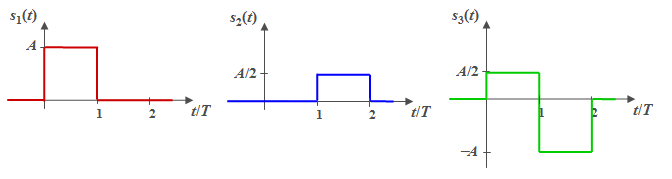
\includegraphics[width=0.7\textwidth]{../Mathematik_2/Bilder/funktionenraum_rechtecksignale_linearkombination.png}
\end{center}
	\begin{itemize}
		\item[(a)] Wie lauten die Abbildungsvorschriften der Signale $s_1, s_2$ und $s_3$?
		\item[(b)] Berechnen Sie die Normen der Signale $s_1$ und $s_2$.
		\item[(c)] Konstruieren Sie aus den Signalen $s_1$ und $s_2$ ein Orthonormalsystem.
		\item[(d)] Zerlegen Sie das Signal $s_3$ bez�glich des Orthonormalsystems und bestimmen Sie die vektoriellen Repr�sentanten der Ausgangssignale bez�glich des Orthonormalsystems.
	\end{itemize}
\vspace{0.3cm}
\textbf{L�sung:} \newline
\begin{itemize}
\item[(a)]
	\begin{eqnarray*}
		s_1: &t\mapsto& \begin{cases} 0, \quad &t\leq 0\,,\\
			A, \quad &0<t\leq 1\,,\\
			0,\quad &t>1\,,
		\end{cases}\\
		s_2: &t\mapsto& \begin{cases} 0, \quad &t\leq 1\,,\\
			A/2, \quad &1<t\leq 2\,,\\
			0,\quad &t>2\,,
		\end{cases}\\
		s_3: &t\mapsto& \begin{cases} 0, \quad &t\leq 0\,,\\
			A/2, \quad &0<t\leq 1\,,\\
			-A, \quad &1<t\leq 2\,,\\
			0,\quad &t>2\,.
		\end{cases}
	\end{eqnarray*}
\item[(b)] Wir berechnen die L�nge der Signale mit dem angegebenen Skalarprodukt:
	\begin{eqnarray*}
		|s_1|^2 &=&  \langle s_1, s_1 \rangle = \int\limits_{-\infty}^\infty s_1(t)\cdot s_1(t) \, \mathrm{d} t = \int\limits_0^1 A^2 \mathrm{d}t = A^2 \;  \Rightarrow |s_1| = |A|\,,\\
		|s_2|^2 &=&  \langle s_2, s_2 \rangle = \int\limits_{-\infty}^\infty s_2(t)\cdot s_2(t) \, \mathrm{d} t = \int\limits_1^2 \left( \dfrac{A}{2} \right)^2\, \mathrm{d}t = \dfrac{A^2}{4} \;  \Rightarrow |s_2| = \left| \dfrac{A}{2}\right|\,.
	\end{eqnarray*}
	Bemerkung: hieran sehen, wir dass die Signale \(s_1\) und \(s_2\) nicht normiert sind.

\item[(c)] Wir �berpr�fen, ob die Signale bez�glich des gegebenen Skalarprodukts orthogonal zueinander sind, indem wir das Skalarprodukt berechnen:
	\[ \langle s_1, s_2 \rangle = \int\limits_{-\infty}^\infty s_1(t) \cdot s_2(t) \,\mathrm d t =  0\,, \]
	Die Intervalle, auf denen die Signale von Null verschieden sind, �berplappen sich nicht und damit ist das Integral null. Die Signale sind orthogonal. Um eine Orthonormalbasis aus \(s_1\) und \(s_2\) zu konstruieren, m�ssen die Signale nur noch normiert werden:

	\[
		\begin{cases}
			\hat s_1(t) = \displaystyle{\frac{ s_1(t)}{|s_1|}} = \displaystyle{\frac{ s_1(t)}{A}}\,,\\
			\hat s_2(t) = \displaystyle{\frac{ s_2(t)}{|s_2|}} = \displaystyle{\frac{ s_2(t)}{A/2}}\,.
	\end{cases} \]
\item[(d)] Das Signal \(s_3\) kann in eine lineare Kombination aus \(\hat s_1\) und \(\hat s_2\) zerlegt werden  \[ s_3(t) = \lambda_1 \cdot \hat s_1(t) + \lambda_2 \cdot \hat s_2(t)\] mit
	\begin{eqnarray*}
		\lambda_1 &=& \langle s_3, \hat s_1\rangle = A/2\\
		\lambda_2 &=& \langle s_3, \hat s_2\rangle = -A
	\end{eqnarray*}

	Die vektoriellen Repr�sentanten der Signale in dem zweidimensionalen Vektorraum, der von den Funktionen $\hat s_1$ und $\hat s_2$ aufgespannt wird, lauten
	\[\boldsymbol s_1 = \left(\begin{array}{c} A\\ 0\end{array}\right), \;
	\boldsymbol s_2 = \left(\begin{array}{c} 0\\ A/2\end{array}\right), \;
\boldsymbol s_3 = \left(\begin{array}{c} A/2\\ -A/2\end{array}\right)\,. \]
	\begin{center}
	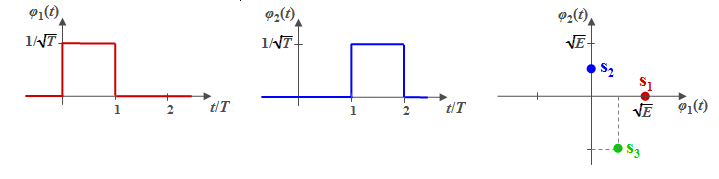
\includegraphics[width=0.7\textwidth]{../Mathematik_2/Bilder/funktionenraum_rechtecksignale_orthonormale_basis.png}
\end{center}
\end{itemize}
\end{exercisebox}


\begin{exercisebox}[Orthogonalit�tsrelationen]
	Berechnen Sie f�r alle $k,l\in\mathbb N_0$ mit $\omega = 2\pi/T$ die folgenden Integrale:
	\begin{eqnarray*}
		(a)\, \int\limits_{0}^{T} \cos(k\omega t) \cdot \cos(l\omega t)\, \mathrm{d}t\,, \quad (b)\, \int\limits_{0}^{T} \sin(k\omega t) \cdot \sin(l\omega t)\, \mathrm{d}t\,,\quad (c)\, \int\limits_{0}^{T} \cos(k\omega t) \cdot \sin(l\omega t)\, \mathrm{d}t
	\end{eqnarray*}
\vspace{0.3cm}
\textbf{L�sung:} \newline
	\begin{eqnarray*}
		&(a)\, &\int\limits_{0}^{T} \cos(k\omega t) \cdot \cos(l\omega t)\, \mathrm{d}t
		= \begin{cases} T, \quad &k=0, \, l=0\,,\\
			T/2, \quad & k=l>0\,,\\
			0, \quad & k\not=l \,,
		\end{cases} \\
		&(b)\, &\int\limits_{0}^{T} \sin(k\omega t) \cdot \sin(l\omega t)\, \mathrm{d}t
		= \begin{cases} T, \quad &k=0, \, l=0\,,\\
			T/2, \quad & k=l>0\,,\\
			0, \quad & k\not=l \,,
		\end{cases} \\
		&(c)\, &\int\limits_{0}^{T} \cos(k\omega t) \cdot \sin(l\omega t)\, \mathrm{d}t = 0\,.
	\end{eqnarray*}
\end{exercisebox}





 \newpage  % Funktionen als Vektoren, Skalarprodukt
% \setcounter{exercise}{0} \section*{Fourier-Polynome und Projektion Aufgaben}\label{MA2-fourierpolynome-und-projektion-loesungen}


\ifintegriereaufgaben Erkl�rungen und Beispiele, die zum Verst�ndnis der L�sungswege hilfreich sind, finden Sie im Skript\wennreferenzvorhanden{MA2-fourierpolynome-und-projektion}{ (Abschnitt \abschnittsverweis{MA2-fourierpolynome-und-projektion})} des Skripts.\fi


\begin{exercisebox}[Bestapproximation] %A.Z. Anwendungen
	Gegeben seien die Funktionen $f_1, f_2, f_3 \in \mathcal C([-\pi,\pi], \mathbb R)$ mit
	\[ f_1: x\mapsto 1, \quad f_2: x\mapsto \cos(x), \quad f_3: x\mapsto \sin(x)\]
	\begin{itemize}
		\item[(a)] Zeigen Sie, dass die Funktionen paarweise orthogonal sind bez�glich des Skalarprodukts
			\[ \langle f, g\rangle : = \int_{-\pi}^{\pi} f(x) \cdot g(x) \, \mathrm{d}x \]
		\item[(b)] Berechnen Sie die Bestapproximation $\tilde f \in \mathcal C([-\pi,\pi],\mathbb R)$ von $f:x\mapsto x^2$ bez�glich $f_i$, $i=1,2,3$ und zeichnen Sie $f$ und $\tilde f$.
		\item[(c)] Zeigen Sie, dass die folgenden Funktionen orthogonal sind\[ \cos(k\cdot x), \, k\in \mathbb N_0, \quad \sin(k\cdot x),  \, k\in \mathbb N\,.\]
	\end{itemize}

\vspace{0.3cm}
\textbf{L�sung:} \newline
\begin{itemize}
	\item[(a)] Die Funktionen sind zueinander orthogonal, denn
		\begin{eqnarray*}
			\langle f_1, f_2\rangle = \int_{-\pi}^\pi \cos(x)\,\mathrm{d}x = \big[ \sin(x) \big]_{-\pi}^\pi  = 0\,,\\
			\langle f_1, f_3\rangle = \int_{-\pi}^\pi \sin(x)\,\mathrm{d}x = \big[ -\cos(x) \big]_{-\pi}^\pi  = 0\,,\\
			\langle f_2, f_3\rangle = \int_{-\pi}^\pi \cos(x)\cdot \sin(x)\,\mathrm{d}x = \big[ \frac12 \sin^2(x) \big]_{-\pi}^\pi  = 0\,.
		\end{eqnarray*}
		Leicht k�nnen wir sie auch normieren:
		\begin{eqnarray*}
			||f_1||^2 &=& 2\pi \Rightarrow \hat f_1: x\mapsto \frac{1}{\sqrt{2\pi}} \\
			||f_2||^2 &=& \pi \Rightarrow \hat f_2: x\mapsto \frac{1}{\sqrt{\pi}} \cos(x)\,,\\
			||f_3||^2 &=& \pi \Rightarrow \hat f_3: x\mapsto \frac{1}{\sqrt{\pi}} \sin(x)\,.
		\end{eqnarray*}
	\item[(b)] Die Bestapproximation von \(f\) bez�glich des Unterraums, der von den Funktionen \( \{ \hat f_1, \hat f_2, \hat f_3\}\) aufgespannt wird lautet:
		\begin{eqnarray*} \tilde f(x) &=& \langle f, \hat f_1\rangle \hat f_1 + \langle f, \hat f_2\rangle \hat f_2  + \langle f, \hat f_3\rangle \hat f_3 \\
		&=& \frac{1}{2\pi} \int\limits_{-\pi}^\pi x^2\,\mathrm{d}x + \frac{1}{\pi} \left(\int\limits_{-\pi}^\pi x^2\cdot \cos(x)\,\mathrm{d}x\right) \cos(x)  + \frac{1}{\pi}\left( \int\limits_{-\pi}^\pi x^2\cdot \sin(x)\,\mathrm{d}x \right) \sin(x)\\
	&=& \frac{\pi^2}{3} - 4\cos(x)\,.\end{eqnarray*}
		Denken Sie daran, dass sich Integrale deren Integrand ein Produkt aus Polynom und trigonometrischer Funktion ist mit mehrfacher partieller Integration l�sen l��t.
	\begin{center}
	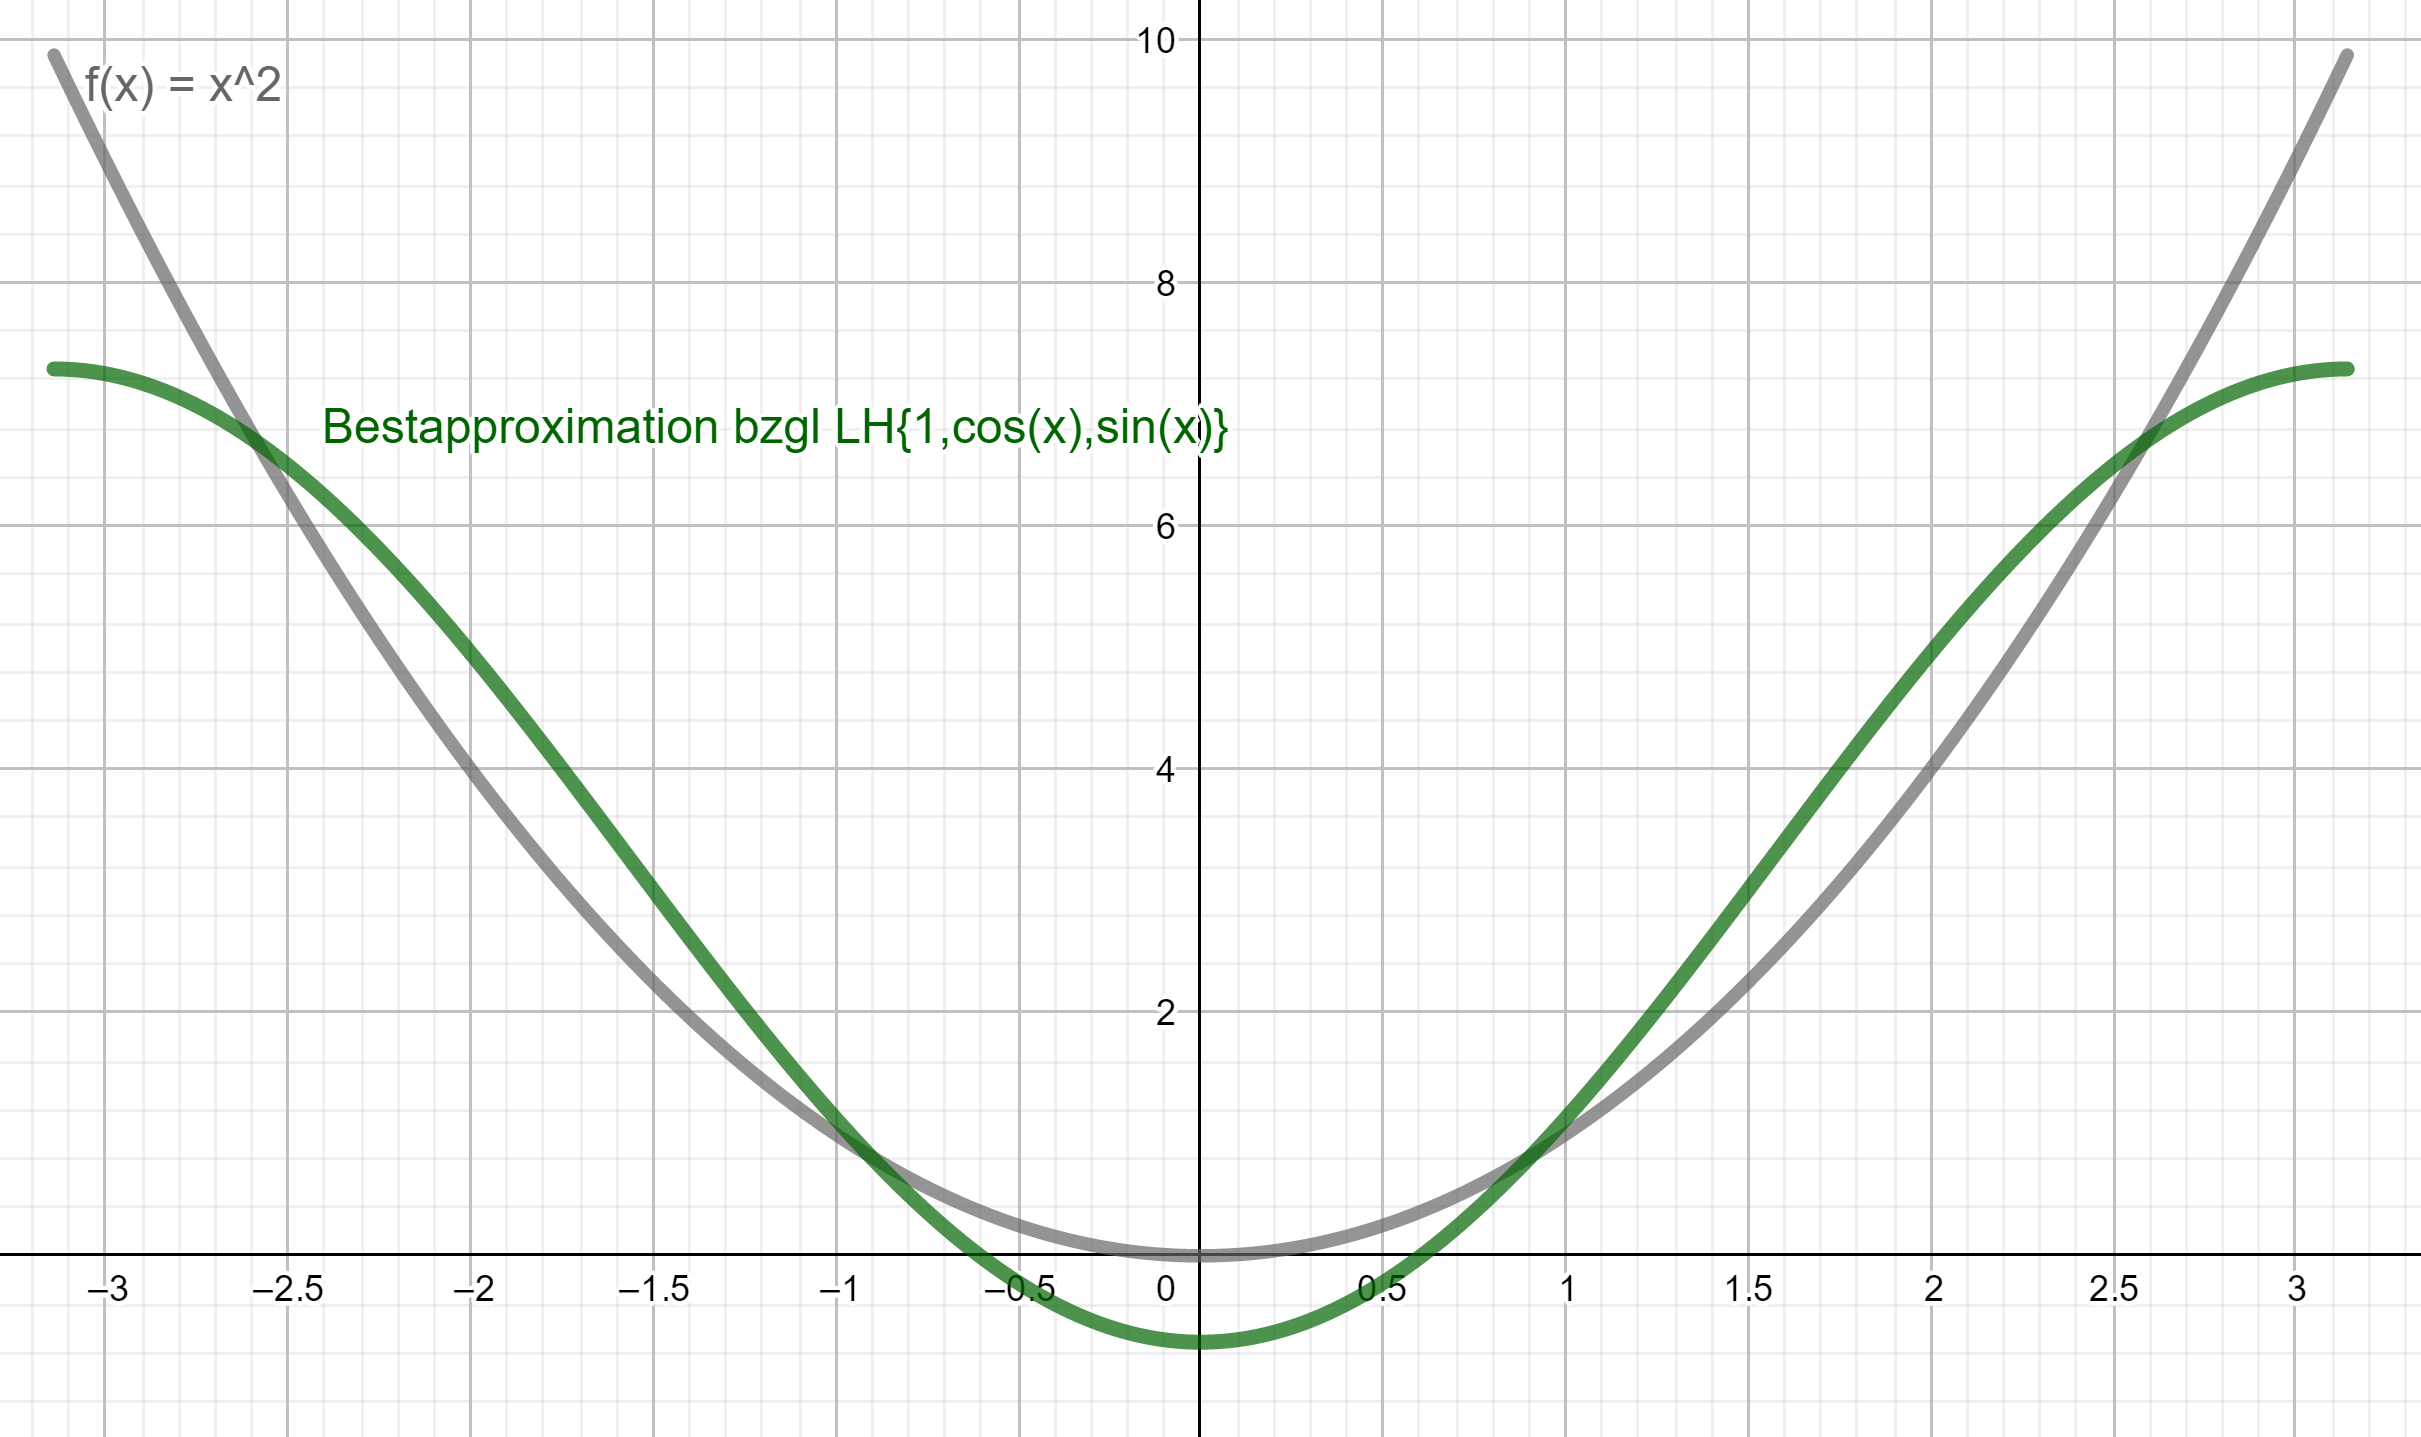
\includegraphics[width=0.8\textwidth]{../Mathematik_2/Bilder/bestapproximation_quadratfunktion_durch_cosinus.png}
\end{center}
	\item[(c)]  Man verwendet die Formeln
		\begin{eqnarray*}
			\cos(\alpha)\cdot \cos(\beta) &=& \frac12 \left( \cos( \alpha - \beta) + \cos(\alpha + \beta)\right) \\
			\sin(\alpha)\cdot \sin(\beta) &=& \frac12 \left( \cos( \alpha - \beta) - \cos(\alpha + \beta)\right) \\
			\sin(\alpha)\cdot \cos(\beta) &=& \frac12 \left( \sin( \alpha - \beta) + \sin(\alpha + \beta)\right)
		\end{eqnarray*}
	\end{itemize}
\end{exercisebox}


\begin{exercisebox}[Bestapproximation]
	Wir betrachten \(\mathcal C([-2,2],\mathbb R)$, den Vektorraum der auf \([-2,2]\) stetigen Funktionen, ausgestattet mit der Maximumsnorm.  Zeigen Sie, dass sich $p$ nicht beliebig genau durch die Funktionen
		\[ f_1(x)=1, \quad f_2(x) = e^x,\quad f_3(x)=e^{2x} \]
		approximieren l��t.

\vspace{0.3cm}
\textbf{L�sung:} \newline
		Offensichtlich liegt $p$ in einem $2$-dimensionalen Unterraum von $\mathcal C([-2,2],\mathbb R)$ und gegeben sind drei linear unabh�ngige Funktionen. W�re $p$ beliebig gut bez�glich der Maximumsnorm approximierbar, dann m�sste sich $p$ also exakt darstellen lassen bez�glich der gegebenen $f_i, i=1,2,3,4$, das hei�t
		\[
		\forall x\in [-2,2]:\quad  x^3-x \stackrel{!}{=} a_0 + a_1e^x + a_2 e^{2x}
	\]
	Es gen�gt eine Auswahl von drei Stellen $x\in [-2,2]$ und wir k�nnen ein lineares Gleichungssystem aufstellen die Zerlegungskoeffizienten $a_i, \, i=0,1,2$ bestimmen. Besonders einfach sind die Nullstellen von $p$: $x_1= 0, x_2 = 1, x_3=-1$.
 \begin{eqnarray*}
	 \begin{cases} 0 \stackrel{!}{=} a_0 + a_1 + a_2 \\
		 0 \stackrel{!}{=} a_0 + a_1 e + a_2 e^2 \\
		 0 \stackrel{!}{=} a_0 + a_1 e^{-1} + a_2 e^{-2}
	 \end{cases}\quad \Rightarrow
	 \left(\begin{array}{ccc|c} 1 & 1 & 1 & 0 \\ 1 & e & e^2 & 0 \\1 e^{-1} & e^{-2} & 0 \end{array}\right) \Leftrightarrow a_i=0, \; i=0,1,2\,.
 \end{eqnarray*}
 Die Approximation ist also $p*: x\mapsto 0$ und damit:
 \[ \| p(x) - p*(x)\|_\infty = 6\,.\]
\end{exercisebox}

 \newpage  % Bestapproximation
% \setcounter{exercise}{0} \section*{Orthogonalprojektion in \(\mathbb R^n\) L�sungen}\label{MA2-orthogonalprojektion-loesungen}

\ifintegriereaufgaben Regeln und Beispiele, die zur Bearbeitung der Aufgaben hilfreich sind, finden Sie im Skript\wennreferenzvorhanden{MA2-orthogonalprojektion}{ (Abschnitt \abschnittsverweis{MA2-orthogonalprojektion})}.\fi

\begin{exercisebox}[�berbestimmtes Gleichungssystem]
test
	\begin{itemize}
		\item[(a)]
	\[ \begin{array}{r c rcl} \textnormal{Ausgangsgleichung} & & \left( \begin{array}{cc}
			2 & 1   \\
			6 & 2   \\
			-1 & 0
	\end{array}\right) \,\left( \begin{array}{c}x_1 \\x_2\end{array}\right) &=&  \left( \begin{array}{c} 1 \\5\\ c \end{array}\right) \\[2ex]
	\textnormal{Trapezform} & \Leftrightarrow &
\left( \begin{array}{cc}
		2 & 1 \\
		0 & -1  \\
		0 & 0
\end{array} \right)\,\left( \begin{array}{c}x_1 \\x_2\end{array}\right) &=&  \left( \begin{array}{c} 1 \\2\\ 2\,c+3 \end{array}\right) \\[2ex] \textnormal{Aufl�sen klappt nur wenn } c=-\frac32 & \Rightarrow & \left(\begin{array}{c} x_1 \\ x_2 \end{array}\right) &=& \begin{cases} \textnormal{keine L�sung}, & \quad c\not=-\frac32\,,\\ \left( \begin{array}{c} 3/2 \\ -2 \end{array}\right), & c=\frac32\,.\end{cases} \end{array}\]
		\item[(b)]
	\[
		\begin{array}{r c rcl} \textnormal{Ausgangsgleichung} & & \left( \begin{array}{cc}
			2 & 1   \\
			6 & 2   \\
			-1 & 0
	\end{array}\right) \,\left( \begin{array}{c}x_1 \\x_2\end{array}\right) &=&  \left( \begin{array}{c} 1 \\5\\ c \end{array}\right) \\[2ex]
	\textnormal{Normalengleichung} &\Rightarrow &
		\left( \begin{array}{cc} 41 & 14 \\ 14 &5
		\end{array}\right) \, \left( \begin{array}{c} x_1 \\ x_2 \end{array}\right) &=& \left( \begin{array}{c} 32-c \\ 11\end{array}\right) \\[2ex] \textnormal{Trapezform} & \Leftrightarrow & \left( \begin{array}{cc} 41 & 14 \\ 0 & 9  \end{array}\right) \, \left( \begin{array}{c} x_1 \\x_2 \end{array}\right) &=& \left( \begin{array}{c} 32-c \\ 3+14\, c \end{array}\right) \\[2ex]

\textnormal{Aufl�sen} & \Leftrightarrow & \boldsymbol x_* =  \left( \begin{array}{c} x_1 \\x_2 \end{array}\right) &=& \frac19\, \left( \begin{array}{c} 6-5\,c \\ 3+14\,c  \end{array}\right) \end{array}\]

		\item[(c)] \[ \begin{array}{r rcl} \textnormal{Residuum} & \boldsymbol r &=& A\,\boldsymbol x_* - \boldsymbol b \\ & &=&\frac19\, \left( \begin{array}{cc}
			2 & 1   \\
			6 & 2   \\
			-1 & 0
\end{array}\right)\left( \begin{array}{c} 6-5\,c \\ 3+14\,c  \end{array}\right) - \left( \begin{array}{c} 1 \\5 \\c \end{array}\right)\\ &&=& \frac19\, \left( \begin{array}{c} 15+4\,c \\ 42-2\,c \\ 6-5\,c \end{array}\right) - \left( \begin{array}{c} 1 \\5 \\c \end{array}\right) \\ &&=& \frac19\,\left( \begin{array}{c} 6+4\,c\\-3-2\,c\\-6-4\,c\end{array}\right) \end{array}\]
Die L�nge des Vektors \(\boldsymbol r\) ist genau dann null, wenn \(\boldsymbol r\) der Nullvektor ist, wenn also jeder Eintrag in \(\boldsymbol r\) null ist: \[\begin{cases} 15+4\,c &= 0 \\ 42-2\,c &= 0 \\ 6-5\,c &= 0\end{cases} \; \Leftrightarrow \; c= -\dfrac32\,.\] Das Residuum wird nur f�r die rechte Seite mit \(c=-3/2\) zum Nullvektor und in diesem Fall war das Gleichungssystem eindeutig l�sbar (siehe (a)) und \(\boldsymbol x_* = \boldsymbol x^*\).
	\end{itemize}
\end{exercisebox}


\begin{exercisebox}[�berbestimmtes Gleichungssystem]
test
	\begin{itemize}
		\item[(a)]
	\[A = \left( \begin{array}{ccc}
			1 & -1 & 1  \\
			3 & 2 & 1  \\
			1 & 2 & 4  \\
			-1 & 7 & 1
\end{array}\right) \]
		\item[(b)] Das Bilds von \(A\) wird aufgespannt durch die linear unabh�ngigen Spaltenvektoren von \(A\). Wie aber findet man die linear unabh�ngigen Spaltenvektoren?

			\begin{enumerate}
				\item Man betrachtet die transponierte Matrix \(A^\intercal\) und bringt \(A^\intercal\) auf Trapezform:
					\[\begin{array}{l c rcl} \textnormal{Ausgangsmatrix} & &A &=& \left( \begin{array}{ccc}
			1 & -1 & 1  \\
			3 & 2 & 1  \\
			1 & 2 & 4  \\
			-1 & 7 & 1
\end{array}\right) \\ \textnormal{Transponierte} & \Rightarrow & A^\intercal &=& \left( \begin{array}{cccc} 1 & 3 & 1 & -1 \\ -1 & 2 & 2 & 7 \\ 1 & 1 & 4 & 1 \end{array}\right) \\ \textnormal{Trapezform} & \Leftrightarrow & & & \left( \begin{array}{cccc} 1 & 3 & 1 & -1 \\ 0 & 5 & 3 & 6 \\ 0 & 0 & 21 & 22 \end{array}\right)\end{array}\]
				\item Die transponierten Zeilenvektoren die nicht, die keine Nullzeilen sind, sind linear unabh�ngig und sie spannen, sobald man sie transponiert, das Bild von \(A\) auf:
					\[\mathrm{im}(A) = \mathrm{LH}\left\{ \underbrace{ \left(\begin{array}{c} 1\\3\\1\\-1\end{array}\right), \; \left( \begin{array}{c} 0\\5\\3\\6\end{array}\right), \; \left( \begin{array}{c} 0 \\ 0 \\21\\22\end{array}\right)}_{\displaystyle{\textnormal{Basisvektoren}}} \right\} \,. \]
					Das Bild von \(\mathcal A\) wird also durch die drei, linear unabh�ngige Vektoren \[ \boldsymbol b_1 = \left(\begin{array}{c} 1\\3\\1\\-1\end{array}\right), \quad \boldsymbol b_2 = \left( \begin{array}{c} 0\\5\\3\\6\end{array}\right), \quad \boldsymbol b_3 = \left( \begin{array}{c} 0 \\ 0 \\21\\22\end{array}\right)\] aufgespannt und damit ist der Rang von \(A\) drei.
			\end{enumerate}
				\item[(c)] Das Gleichungssystem \(A\,\boldsymbol x = \boldsymbol b\) mit \(\boldsymbol b = (0, 2, 0, 2)^\intercal\) ist nicht l�sbar, weil \(\boldsymbol b\) nicht im Bild von \(A\) liegt: \(\boldsymbol b \not\in \mathrm{im}(A)\). Oft �berpr�ft das straight forward: man wendet den Gau�-Algorithmus an und beim R�ckw�rtsaufl�sen der Gleichungen kommt man zu einem unaufl�sbaren Widerspruch:
	\[ \begin{array}{l c rcl} \textnormal{Ausgangsgleichung} & & \left( \begin{array}{ccc}
			1 & -1 & 1  \\
			3 & 2 & 1  \\
			1 & 2 & 4  \\
			-1 & 7 & 1
	\end{array}\right) \,\left( \begin{array}{c}x_1 \\x_2 \\x_3\end{array}\right) &=&  \left( \begin{array}{c} 0 \\2\\0\\2 \end{array}\right) \\[2ex] \textnormal{Trapezform} & \Leftrightarrow &
\left( \begin{array}{ccc}
		1 & -1 & 1 \\
		0 & 5 & -2 \\
		0 & 0 & -7\\
		0 & 0 & -11
\end{array} \right)\,\left( \begin{array}{c}x_1 \\x_2 \\x_3\end{array}\right) &=&  \left( \begin{array}{c} 0 \\2\\ 2\\ 1 \end{array}\right) \\[2ex] \textnormal{Aufl�sen} & \Leftrightarrow & x_3 &=& -\dfrac{1}{11} \land x_3 = -\dfrac{2}{7} \Rightarrow \;\textnormal{unvereinbar} \end{array}\]

\item[(d)] Die Normalengleichung zu \(A\,\boldsymbol x = \boldsymbol b\) lautet \(A^\intercal A \, \boldsymbol x = A^\intercal \,\boldsymbol b\) und die L�sung \(\boldsymbol x_*\) bestimmen wir mit Hilfe des Gau� Algorithmus:
	\[ \begin{array}{l c r cl } \textnormal{Ausgangsgleichung} & & \left( \begin{array}{ccc}
			1 & -1 & 1  \\
			3 & 2 & 1  \\
			1 & 2 & 4  \\
			-1 & 7 & 1
	\end{array}\right) \,\left( \begin{array}{c}x_1 \\x_2 \\x_3\end{array}\right) &=&  \left( \begin{array}{c} 0 \\2\\0\\2 \end{array}\right) \\[2ex]
	\textnormal{Normalengleichung} &\Rightarrow &
		\left( \begin{array}{ccc} 12 & 0 & 7 \\ 0&58&16 \\ 7 &16 & 19
		\end{array}\right) \, \left( \begin{array}{c} x_1 \\ x_2 \\x_3 \end{array}\right) &=& \left( \begin{array}{c} 4 \\ 18 \\ 4\end{array}\right) \\[2ex] \textnormal{Trapezform} & \Leftrightarrow & \left( \begin{array}{ccc} 12 & 0 & 7 \\ 0 & 29 & 8 \\ 0 & 0 & -3655 \end{array}\right) \, \left( \begin{array}{c} x_1 \\x_2\\x_3 \end{array}\right) &=& \left( \begin{array}{c} 4 \\ 9 \\ 1148 \end{array}\right) \\[2ex]

\textnormal{Aufl�sen} & \Leftrightarrow & \boldsymbol x_* = \left( \begin{array}{r} x_1 \\x_2 \\ x_3\end{array}\right) &=& \left( \begin{array}{c} 0.5166 \\ 0.3970 \\ -3.141 \end{array}\right) \end{array}\]

Das Residuum \(\boldsymbol r\) lautet \[\boldsymbol r = A\,\boldsymbol x_* - \boldsymbol b = \left( \begin{array}{r} -0.1945 \\0.0295 \\ 0.0542 \\ -0.0517 \end{array}\right)\,.\] Zwei Vektoren sind senkrecht aufeinander, wenn das Skalarprodukt verschwindet. Da wir eine Basis von \(\mathrm{im}(A)\) bestimmt haben und sich jeder Vektor in \(\mathrm{im}(A)\) als lineare Kombination der Basisvektoren dastellen l�sst, gen�gt es zu zeigen, dass \(\boldsymbol r\) auf jedem der drei Basisvektoren senkrecht steht. Der Matlab-Code (siehe unten) f�hrt zu den folgenden Werten
\[ \begin{array}{rcl}
		\langle \boldsymbol b_1, \boldsymbol r\rangle &=& 0.0372\cdot 1.0e-13 \\
		\langle \boldsymbol b_2, \boldsymbol r\rangle &=& -0.0372\cdot 1.0e-13 \\
\langle \boldsymbol b_3, \boldsymbol r\rangle &=& -0.1044\cdot 1.0e-13 \end{array}\]

\begin{lstlisting}
% Ausgangsdaten
A=[1,-1,1,3;2,1;1,2,4;-1,7,1];
b=[0;2;0;2];

% Basisvektoren f�r im(A) in Matrixdarstellung imA = [b1:b2:b3]
imA = [1,3,1,-1;0,5,3,6;0,0,21,22];

% L�sung der Normalengleichung
x_=A'*A\(A'*b);

% Residuum
r = A*x_-b;

% Pr�fe Orthogonalit�t und gebe das Ergebnis aus
skps = imA*r;
fprintf("Die Skalarprodukte ergeben:\n");
fprintf("<b_1, r> =%d\n", skps[1]);
fprintf("<b_2, r> =%d\n", skps[2]);
fprintf("<b_3, r> =%d\n", skps[3]);
\end{lstlisting}
		\item[(d)] L�sbarkeit eines �berbestimmten Gleichungssystems h�ngt von der rechten Seite ab! Ist der Rang der Matrix \(A\) gleich der Anzahl der Spalten von \(A\), dann ist \(\boldsymbol b \in \mathrm{im}(A)\) notwendig und hinreichend daf�r, dass die die L�sung eindeutig ist. Im vorliegenden Fall gilt \(A \in \mathbb R^{4\times 3}, \mathrm{rang}(A) = 3\) und damit ist \(A\,\boldsymbol x = \boldsymbol b_1\) beispielsweise eindeutig l�sbar. Die eindeutige L�sung lautet \(\boldsymbol x = (1,0,0)^\intercal\).
	\end{itemize}
\end{exercisebox}


\begin{exercisebox}[Koeffizienten Lineare Regression]

	Die lineare Regression ist eine Gerade der Form \(g: x\mapsto g(x) = a_0+a_1\, x\) mit zun�chst unbekannten Koeffizienten \(a_0\) und \(a_1\). Gesucht ist die Funktion, deren Abstandsquadrat in allen Messwerten minimal ist. Die Freiheitsgrade, die zur erf�llung dieser Minimaleigenschaft zur Verf�gung stehen sind die Steigung \(a_0\) und Achsenabschnitt \(a_1\) von \(g\). Die Aufgabe lautet auf mathematisch also: bestimme den Vektor aus Koeffizienten \[ \boldsymbol a = \left( \begin{array}{c} a_0 \\a_1\end{array}\right)\] genau so, dass die Funktion \[ E: \boldsymbol a \mapsto  \sum\limits_{i=1}^n \left( \left( a_0 + a_1\, x_i\right) - y_i \right)^2 \] minimal wird. \(E\) h�ngt von zwei Variablen ab und damit ist die Ableitung der Gradient. Die Eintr�ge des Gradient \(\nabla E\) sind die zwei partielle Ableitungen von \(E\) und die k�nnen wir explizit bestimmen:
	\[\begin{array}{rcl } \dfrac{\partial E(\boldsymbol a)}{\partial a_0} &=& \dfrac{\partial }{\partial a_0} \, \left( \displaystyle\sum\limits_{i=1}^n \left( \left( a_0 + a_1\, x_i\right) - y_i \right)^2 \right) = \displaystyle\sum\limits_{i=1}^n \dfrac{\partial }{\partial a_0} \left( \left( a_0 + a_1\, x_i\right) - y_i \right)^2  \\  &=& \displaystyle\sum\limits_{i=1}^n 2\cdot \left( \left( a_0 + a_1\, x_i\right) - y_i \right) \cdot 1 = 2\, \displaystyle\sum\limits_{i=1}^n \left( \left( a_0 + a_1\, x_i\right) - y_i \right)\,, \\[2ex] \dfrac{\partial E(\boldsymbol a)}{\partial a_1} &=& \dfrac{\partial }{\partial a_1} \left( \displaystyle\sum\limits_{i=1}^n \left( \left( a_0 + a_1\, x_i\right) - y_i \right)^2 \right) = \displaystyle\sum\limits_{i=1}^n \dfrac{\partial }{\partial a_1}\, \left( \left( a_0 + a_1\, x_i\right) - y_i \right)^2  \\  &=& \displaystyle\sum\limits_{i=1}^n 2\cdot \left( \left( a_0 + a_1\, x_i\right) - y_i \right) \cdot x_i = 2\, \displaystyle\sum\limits_{i=1}^n \left( \left( a_0 + a_1\, x_i\right) - y_i \right)\cdot x_i \,. \end{array}\]
			Genauso wie bei Funktionen, die nur von einer Variable abh�ngen, ist die notwendige Bedingung f�r ein lokales Extremum das Verschwinden der Ableitung: \[ \boldsymbol a \textnormal{ Minimium von } E \; \Rightarrow \nabla E(\boldsymbol a) = \boldsymbol 0 \; \Leftrightarrow \dfrac{\partial E}{\partial a_0} = 0\,; \land \; \dfrac{\partial E}{\partial a_1}= 0\,.\]
			F�r welchen Vektor verschwinden die partiellen Ableitung? Setzen wir sie zu null und l�sen auf:
			\[ \begin{array}{c rcl c rcl}
					& \dfrac{\partial E(\boldsymbol a)}{\partial a_0} &=& 0  \\ \Leftrightarrow & 2\, \displaystyle\sum\limits_{i=1}^n \left( \left( a_0 + a_1\, x_i\right) - y_i \right) &=&0 \\\Leftrightarrow &  2 \,\underbrace{ \displaystyle\sum\limits_{i=1}^n a_0 }_{\displaystyle{ = n\, a_0}}  + 2\,a_1 \underbrace{ \displaystyle\sum\limits_{i=1}^n x_i}_{\displaystyle{ = n\, \overline x} }  - 2  \underbrace{ \displaystyle\sum\limits_{i=1}^n y_i}_{\displaystyle{ = n\, \overline y} } &=& 0 \\ \Leftrightarrow & 2\,n\, \left( a_0 + a_1 \, \overline x - \overline y\right) &=&0 & \Leftrightarrow & a_0 &=& \overline y - a_1 \, \overline x\,, \\ [2ex]
					& \dfrac{\partial E(\boldsymbol a)}{\partial a_1} &=& 0 \\ \Leftrightarrow &  2\, \displaystyle\sum\limits_{i=1}^n \left( \left( \textcolor{blue}{a_0} + a_1\, x_i\right) - y_i \right)\cdot x_i &=&0 \\ \Leftrightarrow & 2\, \displaystyle\sum\limits_{i=1}^n \left( \left( \textcolor{blue}{ \overline y - a_1 \, \overline x} + a_1\, x_i\right) - y_i \right)\cdot x_i &=&0 \\ \Leftrightarrow& 2\, \displaystyle\sum\limits_{i=1}^n \left(\overline y - y_i\right) \cdot x_i + a_1\, \displaystyle \sum\limits_{i=1}^n \left( x_i - \overline x \right)\cdot x_i &=& 0\\ \Leftrightarrow & 2\,\displaystyle \sum\limits_{i=1}^n \left( \left(\overline y - y_i\right) \cdot x_i + a_1\,\left( x_i- \overline x \right)\cdot x_i \right) &=& 0 & \Leftrightarrow & a_1 &=& \dfrac{\displaystyle \sum\limits_{i=1}^n \left( y_i -\overline y \right)\cdot x_i}{\displaystyle \sum\limits_{i=1}^n \left(x_i - \overline x \right)\cdot x_i} \,.
			\end{array}\]
			Zu der in der Aufgabenstellung angegebenen Formel gelangt man durch einen Trick:
			\[\begin{array}{rcl}
					\sum\limits_{i=1}^n \left(y_i -\overline y\right) \cdot x_i &=&  \sum\limits_{i=1}^n \left(y_i - \overline y\right) \cdot \left( x_i \textcolor{blue}{- \overline x}\right) \textcolor{blue}{+} \underbrace{ \sum\limits_{i=1}^n  \left( y_i - \overline y \right) \cdot \textcolor{blue}{\overline x} }_{\displaystyle{= 0}}  =  \sum\limits_{i=1}^n \left( y_i - \overline y \right) \cdot \left( x_i - \overline x\right) \\
		\sum\limits_{i=1}^n \left(x_i - \overline x \right) \cdot x_i &=&  \sum\limits_{i=1}^n \left(x_i - \overline x\right) \cdot \left( x_i \textcolor{blue}{- \overline x}\right) \textcolor{blue}{+} \underbrace{ \sum\limits_{i=1}^n  \left(x_i - \overline x\right) \cdot \textcolor{blue}{\overline x} }_{\displaystyle{= 0}}  =  \sum\limits_{i=1}^n \left(x_i - \overline x \right) \cdot \left( x_i - \overline x\right) \end{array}\]

\end{exercisebox}

\begin{exercisebox}[L�sung der Normalengleichung]
test
	\begin{itemize}
	\item[(i)] Das Residuum \(\boldsymbol r = A\,\boldsymbol x - \boldsymbol b\) h�ngt von \(\boldsymbol x\in\mathbb R^m\) ab und entsprechend ist \( \|\boldsymbol r\|^2 \) eine Funktion, die von \(\boldsymbol x\) abh�ngt. Machen wir das explizit und definieren diese Funktion:
		\[ E: \mathbb R^m \to \mathbb R, \boldsymbol x \mapsto \sum\limits_{i=1}^n r_i^2, \quad r_i = \left(A \boldsymbol x - \boldsymbol b\right)_i\,.\] Die Behauptung, die zu zeigen ist, lautet jetzt wie folgt: wenn \(\boldsymbol x_*\) eine Minimalstelle von \(E\) ist, dann l�st \(\boldsymbol x_*\) die Normalengleichung. Notwendig daf�r, dass \(E\) in \(\boldsymbol x_*\) ein Minimum besitzt, ist das Verschwinden des Gradienten an der Stelle \(\boldsymbol x_*\):
		\[ \nabla E(\boldsymbol x_*) = \boldsymbol 0 \; \Leftrightarrow  \; \dfrac{\partial E(\boldsymbol x_*)}{\partial x_k} = 0 \; \textnormal{f�r } k=1,\cdots,m\,.\] Die Funktion \(E\) h�ngt von \(m\) Variablen ab und damit gibt es \(m\) partielle Ableitungen und jede der partiellen Ableitung l�sst sich exakt berechnen
\[ \begin{array}{rcl l}  k=1,\cdots,m:\quad \dfrac{\partial E(\boldsymbol x)}{\partial x_k} &=&
	\dfrac{\partial}{\partial x_k} \, \displaystyle \sum\limits_{i=1}^n r_i^2  & \quad\textnormal{summandenweise ableiten} \\[2ex]
		&=&\displaystyle \sum\limits_{i=1}^n \dfrac{\partial}{\partial x_k} r_i^2 & \quad \textnormal{Kettenregel anwenden}\\[2ex]
		&=& \displaystyle \sum\limits_{i=1}^n 2\cdot r_i\cdot \dfrac{\partial }{\partial x_k} r_i & \quad\quad\bullet \textnormal{ �u�ere Ableitung}\\[2ex]
		&=& 2\cdot \displaystyle \sum\limits_{i=1}^n r_i \cdot a_{ki} &  \quad\quad \bullet\textnormal{ innere Ableitung}  \\[2ex]
&=& 2\cdot \left( A^\intercal\, \boldsymbol r\right)_k &\quad \textnormal{Matrix-Vektor-Multiplikation identifizieren} \end{array}\]
Der Gradient von \(E\) lautet also \[ \nabla E(\boldsymbol x) = 2\cdot A^\intercal \, \boldsymbol r = 2\cdot A^\intercal \, \left( A \, \boldsymbol x - \,\boldsymbol b\right)\]
Nehmen wir an, dass \(g\) in \(\boldsymbol x_*\) ein lokales Minimum besitzt, dann muss \(\boldsymbol x_*\) die Normalengleichung l�sen:
\[\begin{array}{l crcl l} \textnormal{Ableitung verschwindet}&  &\nabla E(\boldsymbol x_*) &=& \boldsymbol 0 &\\  & \Leftrightarrow  & 2\, A^\intercal \, \left( A \, \boldsymbol x_* - \boldsymbol b\right)  &=& 0 &\|\cdot\frac12 \\[1ex] & \Leftrightarrow &  A^\intercal \, A \, \boldsymbol x_* - A^\intercal \,\boldsymbol b&=& 0 &\| + A^\intercal \, \boldsymbol b \\[1ex] \textnormal{Normalengleichung erf�llt} &  \Leftrightarrow &  A^\intercal \, A \, \boldsymbol x_* &=& A^\intercal \,\boldsymbol b &\end{array}\]

\item[(ii)] Ist \(\boldsymbol x_*\) L�sung der Normalengleichung, dann ist sein Residuum \(\boldsymbol r\) immer senkrecht auf dem Bild von \(A\):
		\[\begin{array}{l c rcl r}\textnormal{Normalengleichung:} & & A^\intercal \, A \, \boldsymbol x_* &=& A^\intercal \, \boldsymbol b &\| -A^\intercal\,\boldsymbol b \\ &\Leftrightarrow & A^\intercal \,\left(\textcolor{blue}{ A\,\boldsymbol x_* - \boldsymbol b}\right) &=& \boldsymbol 0 & \\ &\Leftrightarrow & A^\intercal \,\textcolor{blue}{ \boldsymbol r} &=& \boldsymbol 0 & \Rightarrow\; \textcolor{blue}{\boldsymbol r} \in \mathrm{ker}\left(A^\intercal\right) \\[2ex] \textnormal{Schlussfolgerung:}\quad \forall\, \boldsymbol x\in \mathbb R^n: && \langle A^\intercal \, \boldsymbol r, \boldsymbol x \rangle &=& \langle \boldsymbol 0, \boldsymbol x\rangle & \\ &\Leftrightarrow& \langle \boldsymbol r, A\,\boldsymbol x\rangle &=& 0 &\Rightarrow\quad  \boldsymbol r \perp \mathrm{im}(A)\,.
		\end{array}\]
		%\[\Rightarrow \; \mathrm{im}(A) = \left( \mathrm{ker}(A^\intercal)\right)^\perp \]
\end{itemize}
\end{exercisebox}

 \newpage  % �berbestimmte GL, Normalengleichung, Ausgleichsgerade
%
% \setcounter{exercise}{0} \section*{Fourierreihen Aufgaben mit L�sungen}\label{MA2-fourierreihen-loesungen}

\ifintegriereaufgaben Erkl�rungen und Beispiele, die zum Verst�ndnis der L�sungswege hilfreich sind, finden Sie im Skript\wennreferenzvorhanden{MA2-fourierreihen}{ (Abschnitt \abschnittsverweis{MA2-fourierreihen})}. \fi

	\begin{exercisebox}[Harmonische Schwingungen]
		Bestimmen Sie die Amplitude, die Periode und die Nullphase der folgenden harmonischen Schwingungen und skizzieren sie den Funktionsverlauf
		\begin{eqnarray*}
		(a)\; y(t) = \textcolor{red}{2\,\sin\left(3\, t-\dfrac{\pi}{6} \right)}\quad \quad (b)\; y(t) = \textcolor{blue}{10\,\sin\left(\pi\, t - 3\,\pi\right)}\,.
		\end{eqnarray*}
\vspace{0.3cm}
\noindent \textbf{L�sung:}
\vspace{0.3cm}

	\begin{minipage}{0.6\textwidth}
	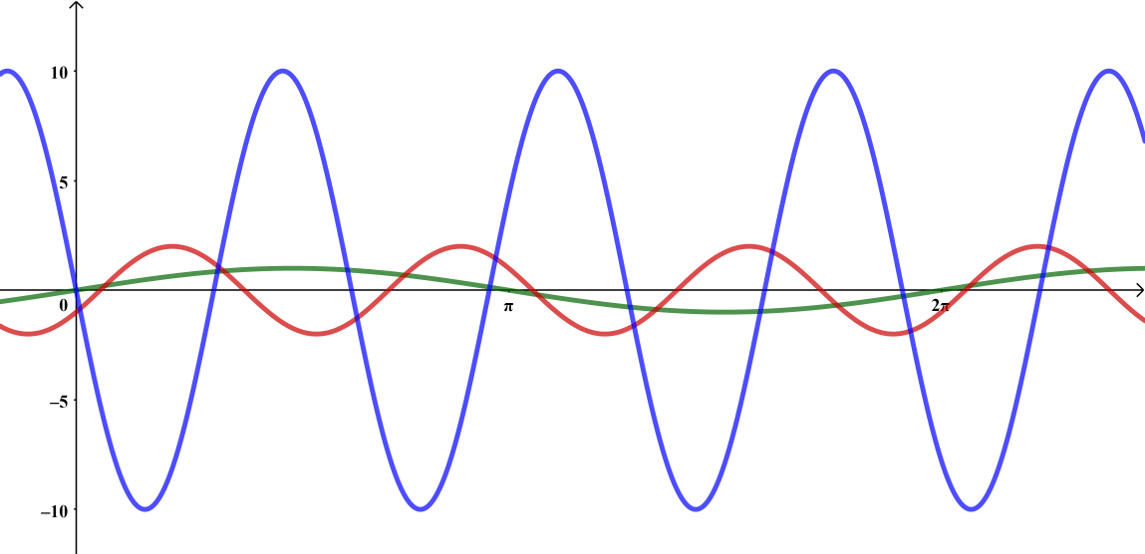
\includegraphics[width=\textwidth]{../Mathematik_2/Bilder/harmonische_schwingungen_amplitude_periode_phase.png}
\end{minipage}
	\begin{minipage}{0.4\textwidth}
		\begin{itemize}
			\item[(a)]  $\textcolor{red}{A=2, \, T= \dfrac{2\pi}{3}, \, \varphi_0 = -\dfrac{\pi}{6} }$
			\item[(b)]  $\textcolor{blue}{A=10, \, T= 2, \, \varphi_0 = -3\pi }$
				\item[(c)] \( \textcolor{darkgreen}{ A=1, \, T= 2\pi, \, \varphi_0 = 0 } \) \newline (Sinus-Funktion zum Vergleich)
\end{itemize}
\end{minipage}

\end{exercisebox}

	\begin{exercisebox}[komplexes Fourier-Polynom vs. reelles Fourier-Polynom]
		\begin{itemize}
			\item[(a)]
		Man kann die komplexwertigen Koffizienten $c_k$ eines komplexen Fourier Polynoms
		\[
			p_{N,f}(t) = \sum\limits_{k=-N}^N c_k\cdot e^{i\,k\,\omega_0\, t} \,,
		\]
		in die reell-wertigen Koeffizienten $a_n$ und $b_n$ des entsprechenden reellen Fourier-Polynom umrechnen und das funktioniert wie folgt:

		\begin{equation}\label{a_k_zu_c_k}
			\left\{ \begin{array}{rcl}
				a_0 & = &  2\, c_0, \\[1ex]
				a_n & = & c_n + c_{-n},\\[1ex]
				b_n & = & i \, \left( c_{-n} + c_{n}\right) \,.
		\end{array}\right.
	\end{equation}
\item[(b)]
		Man kann die reellen Koffizienten eines Fourier Polynoms
		\[
			p_{N,f}(t) = \frac{a_0}{2} + \sum\limits_{n=1}^N\left( a_n\cdot \cos( n \, \omega_0 \, t) + b_n \cdot \sin(n \, \omega_0\, t)\right)\,,
		\]
		in die komplex-wertigen Koeffizienten $c_k$ des entsprechend komplex-wertigen Fourier-Polynoms umrechnen und das funktioniert wie folgt:
		\begin{eqnarray*}
			&& \begin{cases}
				c_0 = \frac12\, a_0,\\[1ex]
				c_n = \frac12\, \left( a_n - i\, b_n\right) , \quad n \in \mathbb N^+\,, \\[1ex]
			c_{-n} = \frac12 \, \left( a_n + i \, b_n\right),\quad  , \quad n \in \mathbb N^+\,. \end{cases}
	\end{eqnarray*}
	\end{itemize}
\end{exercisebox}


\begin{exercisebox}[Fourier-Reihen]
	Skizzieren Sie zun�chst die Funktionen und berechnen Sie anschlie�end die Fourier-Reihen.
	\begin{itemize}
		\item[(a)] Periode $T=2$ und
			\[ f(t) = t, \quad t \in [0,2]\,.\]
		\item[(b)] Periode $T=1$ und
			\[ f(t) = |t|, \quad t \in \left[-\frac12,\frac12\right]\,.\]
		\item[(c)] Periode $T>0$ und
			\[ f(t) = t\cdot (T-t), \quad t \in [0,T]\,.\]
		\item[(d)] Periode $T=2\pi$ und
			\[ f(t) = \max(\sin(t),0), \quad t \in [0,2\pi]\,.\]

	\end{itemize}
\vspace{0.3cm}
\noindent \textbf{L�sung:}

\begin{itemize}
	\item[(a)] Eine Skizze des Signals zeigt, dass \(f\) um die horizontale Gerade \( x\mapsto 1\) schwingt. Aus dieser Beobachtung folgt, dass der konstante Anteil der Fourierreihe, also der Summand \(a_0/2\) bzw. \(c_0\), den Zahlenwert eins hat. Bez�glich des Punkts \( (1|0)\) ist \(f\) punktsymmetrisch und damit ein ungerades Signal. Die Fourierkoeffizienten lauten
		\begin{eqnarray*} \begin{cases} a_0 = 2, \quad &\\
				a_k = 0, \quad &k>0, \\
				b_k = -\displaystyle{\frac{2}{\pi k}}, \quad &k>0\,.
			\end{cases}
		\end{eqnarray*}
		Die Periode \(T\) definiert die Grundfreqzenz \(\omega_0 = \dfrac{2\pi}{T} = \pi\) und damit erhalten wir
		\begin{eqnarray*}
			\mathrm{FR}_f(t) = \frac{a_0}{2} + \sum\limits_{k=1}^\infty a_k\cdot\cos( k\,\omega_0\, t) + b_k\cdot \sin(k\,\omega_0\,t) =  1 - \sum\limits_{k=1}^\infty \frac{2}{k \,\pi} \cdot \sin(k \, \pi \,t) \,.
		\end{eqnarray*}

		\vspace{0.2cm}
		\noindent\textbf{Bemerkung:}
		Entwickelt man anstatt der reellen Fourierreihe die komplexe Fourierreihe, dann kann es sein, dass die Fourierreihen auf den ersten Blick nicht dieselbe Form haben. Entweder kann man die Reihen auf Gleichheit �berpr�fen, indem man �berpr�ft, ob die Umrechnungsformel \eqref{a_k_zu_c_k} wahr sind. Eine Alternative ist die komplexe Reihe in eine reelle Reihe umzuformen. Letzteres klappt wie folgt
		\begin{itemize}
			\item Komplexe Reihe in drei Teile aufspalten \[ \mathrm{FR}_f(t) = \sum\limits_{-\infty}^\infty c_k\cdot e^{i \, k \, \omega_0\,t} = \sum\limits_{k=-\infty}^{k=-1} c_k\cdot e^{i\, k \, \omega_0\, t} + c_0 + \sum\limits_{k=1}^\infty c_k\cdot e^{i \, k\, \omega_0\, t} \]
			\item Summanden der Reihe umsortieren: \[ \mathrm{FR}_f(t) = c_0 + \sum\limits_{k=1}^\infty \left( c_k\cdot  e^{i \, k\,\pi\, t} + c_{-k}\cdot e^{-i \, k \, \pi\, t} \right) \]
			\item Komplex konjugierte Zahlen identifizieren
				\[ \mathrm{FR}_f(t) = c_0 + \sum\limits_{k=1}^\infty \left(  c_k\cdot e^{i \, k\,\pi\, t} + \overline { c_{k} \cdot e^{i \, k\, \pi \, t} } +\right)\,, \] wobei
				\begin{eqnarray*} c_{-k} &=& \overline{ c_k} \,,\\ e^{-i \, k\,\omega_0\, t} &=& \overline{ e^{i \, k \omega_0\, t} }\,, \\\Rightarrow c_{-k}\cdot e^{-i\, k\, \omega_0\, t} &=& \overline{ c_k \cdot e^{i \, k \,\omega_0\,t}}\,.\end{eqnarray*}
			\item Reelle und imagin�re Anteile trennen und Eulersche Identit�ten
				\begin{eqnarray*}
					\cos\left(k\, \omega_0\, t\right) &=& \frac12\cdot \left( e^{i\, k\,\omega_0\, t} + e^{-i\, \, k \, \omega_0\,t} \right) \,,\\
				\sin\left( k \, \omega_0 \, t\right) &=& -\frac{i}{2}\, \left( e^{i\, k\,\omega_0\,t } - e^{-i\, \, k\,\omega_0\,t } \right) \,.\end{eqnarray*}

				anwenden.
		\end{itemize}
	\item[(b)] $f$ ist achsensymmetrisch (gerade) mit Periode \(T = 1\), also Grundschwingung \(\omega_0 = \dfrac{2\pi}{T} = 2\pi\) . Die Fourierkoeffizienten sind
		\begin{eqnarray*} \begin{cases} a_0 &= \displaystyle{\frac12}\,,\\
				a_k &= \displaystyle{\frac{(-1)^k - 1 }{\pi^2 k^2} } = \begin{cases} 0,  &\quad k \; \textnormal{gerade}, \\ \displaystyle{\frac{-2}{\pi^2 k^2} }, & \quad k \; \textnormal{ungerade}\,,\end{cases}\\
				b_k &= 0\,, \quad \textnormal{f�r alle } k\geq 1\,.
			\end{cases}
			\end{eqnarray*}
			Die Funktion l��t sich also allein durch Kosinus-Schwingungen rekonstruieren, alle \(b_k\) sind null. Weiterhin tauchen nur Frequenzen auf mit ungeradem Index:  \[a_{2k-1}= - \dfrac{2}{\pi^2 ( 2k-1)^2}, \quad k = 1,\cdots \,.\]
			\begin{eqnarray*}
				\Rightarrow\quad  \mathrm{FR}_f(t) &=& \dfrac{a_0}{2} + \sum\limits_{k=1}^\infty a_k\cdot \cos\left( k \, \omega_0\, t\right) + b_k\cdot \sin\left( k \,\omega_0\, t\right) \\
				&=& \dfrac14 + \sum\limits_{k=1}^\infty \dfrac{-2}{\pi^2\,(2\,k-1)^2} \cdot \cos(2\pi\,(2\,k-1)\, t) \\
				&=& \frac14 - \frac{2}{\pi^2} \left( \frac{\cos(2\pi\, t)}{1^2} + \frac{\cos(3\cdot 2\pi\, t)}{3^2} + \frac{\cos(5\cdot 2\pi\, t)}{5^2} + \dots \right)
		\end{eqnarray*}
	\item[(c)] $f$ ist achsensymmetrisch (gerade) mit Periode \(T\) und Grundschwingung \(\omega_0 = \dfrac{2\pi}{T}\). Die Fourierkoeffizienten lauten
		\begin{eqnarray*}
			\begin{cases} a_0 = \displaystyle{\frac{T^2}{3}}, \quad &\\
				a_k = -\displaystyle{\frac{T^2 }{\pi^2 k^2} }, \quad &k>0, \\
				b_k = 0, \quad &k>0\,.
			\end{cases}
			\end{eqnarray*}
			\begin{eqnarray*}
				\Rightarrow\quad \mathrm{FR}_f(t) &=& \frac{T^2}{6} - \frac{T^2}{\pi^2} \sum\limits_{k=1}^\infty \frac{1}{k^2} \cos\left(k \, \omega_0\,t\right) \\
				&=& \frac{T^2}{6} - \frac{T^2}{\pi^2}\cdot \left( \frac{\cos(\omega_0\, t)}{1^2} + \frac{\cos(2\cdot \omega_0\, t)}{2^2} + \frac{\cos(3\cdot \omega_0\, t)}{3^2} + \dots \right)
		\end{eqnarray*}
	\item[(d)] $f$ ist \(\pi\)-periodisch und weder gerade noch ungerade. Die Fourierkoeffizienten lauten
		\begin{eqnarray*}
			\begin{cases} a_0 = \displaystyle{\frac{2}{\pi}}, \quad &\\
				a_k = -\displaystyle{\frac{(-1)^k+1 }{\pi k^2 -\pi} }, \quad &k>0, \\
				b_1 = \displaystyle{\frac12} \,, & \\
				b_k = 0 \,, & k>1
			\end{cases}
			\end{eqnarray*}
			\begin{eqnarray*}
				\omega_0 = 2\; \Rightarrow\quad \mathrm{FR}_f(t) &=& \frac{1}{\pi} + \frac{1}{2}\sin(t) + \frac{2}{\pi}\cdot \sum\limits_{k=1}^\infty \frac{1}{(2k)^2-1 }\cdot \cos\left(2\,k\, t\right) \\
				&=& \frac{1}{\pi} + \frac{1}{2}\cdot \sin(t) + \frac{2}{\pi}\cdot \left( \frac{\cos(2 \,t)}{2^2-1} + \frac{\cos(4\, t)}{4^2-1} + \frac{\cos(6\, t)}{6^2-1} + \dots \right)
		\end{eqnarray*}
	\end{itemize}
\end{exercisebox}


%\begin{exabox}{\hyperlink{Aufabe_8.6}{Interpolationseigenschaft}}{ }
%Um uns davon zu �berzeugen, setzen wir \(\tilde c_k\) ein,
%\begin{eqnarray*}
%	g_n(t_j) &=& \dfrac{1}{n} \sum\limits_{k=0}^{n-1} \tilde c_k e^{i k \omega_0 t_j } \\[2ex]
%	%&=& \sum\limits_{k=0}^{n-1} \textcolor{blue}{\tilde c_k} e^{i k \, 2\pi/(n\cdot h)\, j\cdot h }\\[2ex]
%	&=& \sum\limits_{k=0}^{n-1} \textcolor{blue}{\tilde c_k} e^{i k \, 2\pi/n\, j } \\[2ex]
%	&=& \sum\limits_{k=0}^{n-1}  \textcolor{blue}{ \dfrac1n \sum\limits_{l=0}^{n-1} f_l \cdot e^{-i \, k\, 2\pi\, l/n} } e^{i k \, 2\pi/n\, j } \\[2ex]
%	&=& \textcolor{blue}{\dfrac{1}{n} \sum\limits_{l=0}^{n-1} f_l} \sum\limits_{k=0}^{n-1} \textcolor{blue}{ e^{-i \, k\, 2\pi\, l/n} } e^{i k \, 2\pi/n\, j } \\[2ex]
%	&=& \dfrac{1}{n} \sum\limits_{l=0}^{n-1} f_l \sum\limits_{k=0}^{n-1} e^{i 2\pi\, (j-l)k/ n} \\[2ex]
%	&\stackrel{(*)}{=}& \dfrac{1}{n} \sum\limits_{l=0}^{n-1} f_l \cdot n \cdot \delta_{lj} \\[2ex]
%	&=& f_j\,.
%\end{eqnarray*}
%\((*)\) folgt aus der folgenden Beobachtung:
%\[ \sum\limits_{k=0}^{n-1} e^{i \,2\pi (j-l) k/n} = \sum\limits_{k=0}^{n-1} \left( z^{j-l}\right)^k = n\cdot \delta_{jl} = \begin{cases} n,\quad j= l\,,\\ 0,\quad j\not=l\,, \end{cases} \]
%	wobei sich das letzte Ergebnis im Detail wie folgt zeigen l��t
%	\begin{itemize}
%		\item f�r \(j=l\) wird der Exponent in jedem Summand null und damit \[\sum\limits_{k=0}^{n-1} z^{0\cdot k} = \sum\limits_{k=0}^{n-1} 1 = n\,.\]
%		\item f�r \(j\not=l\) ist der Wert der Summe null. Die \(n\)-te Potenz einer beliebigen Einheitswurzel \(Z\) ist eins und damit
%			\[ \sum\limits_{k=0}^{n-1} Z^k = 1 + Z + Z^2 + \cdots + Z^{n-1} = \dfrac{ Z^n -1}{Z-1} = \dfrac{1-1}{Z-1} = 0\,.\]
%	\end{itemize}
%
%	Wenn man f�r ein gegebenes diskretes Spektrum die Messwerte des Signals berechnet, f�hrt invertiert man quasi den Zerlegungsprozess. Man nennt das Verfahren die inverse Diskrete Fouriertransformation [iDFT].
%	Zusammen lauten die Formeln
%	\begin{eqnarray*}
%		\textnormal{DFT:}\quad \{f_j\}_{j=0}^{n-1} &\mapsto& \{\tilde c_j\}_{j=0}^{n-1}\,, \\
%		\tilde c_j &=& \dfrac{1}{n} \sum\limits_{k=0}^{n-1} f_k e^{- i \, k 2\pi \,j/n}\,, \quad j=0,\cdots,n-1\,,\\
%		\textnormal{iDFT:}\quad \{\tilde c_j\}_{j=0}^{n-1} &\mapsto& \{f_j\}_{j=0}^{n-1}\,, \\
%		f_j &=& \sum\limits_{k=0}^{n-1} \tilde c_k e^{i \, k 2\pi \,j/n}\,, \quad j=0,\cdots,n-1\,.
%	\end{eqnarray*}
%\end{exabox}


 \newpage
% \setcounter{exercise}{0} \section*{Diskrete Fouriertransformation L�sungen}\label{MA2-diskrete-fouriertransformation-loesungen}

\ifintegriereaufgaben  Regeln und Beispiele, die zum Verst�ndnis der L�sungswege hilfreich sind, finden Sie im Skript\wennreferenzvorhanden{MA2-diskrete-fouriertransformation}{ (Abschnitt \abschnittsverweis{MA2-diskrete-fouriertransformation})}. \fi

\begin{exercisebox}{Orthogonalit�t}{ }
\begin{itemize}
\item[(a)]
	\begin{eqnarray*}
		s_1: &t\mapsto& \begin{cases} 0, \quad &t\leq 0\,,\\
			A, \quad &0<t\leq 1\,,\\
			0,\quad &t>1\,,
		\end{cases}\\
		s_2: &t\mapsto& \begin{cases} 0, \quad &t\leq 1\,,\\
			A/2, \quad &1<t\leq 2\,,\\
			0,\quad &t>2\,,
		\end{cases}\\
		s_3: &t\mapsto& \begin{cases} 0, \quad &t\leq 0\,,\\
			A/2, \quad &0<t\leq 1\,,\\
			-A, \quad &1<t\leq 2\,,\\
			0,\quad &t>2\,.
		\end{cases}
	\end{eqnarray*}
\item[(b)] Wir berechnen die L�nge der Signale mit dem angegebenen Skalarprodukt:
	\begin{eqnarray*}
		|s_1|^2 &=&  \langle s_1, s_1 \rangle = \int\limits_{-\infty}^\infty s_1(t)\cdot s_1(t) \, \mathrm{d} t = \int\limits_0^1 A^2 \mathrm{d}t = A^2 \;  \Rightarrow |s_1| = |A|\,,\\
		|s_2|^2 &=&  \langle s_2, s_2 \rangle = \int\limits_{-\infty}^\infty s_2(t)\cdot s_2(t) \, \mathrm{d} t = \int\limits_1^2 \left( \dfrac{A}{2} \right)^2\, \mathrm{d}t = \dfrac{A^2}{4} \;  \Rightarrow |s_2| = \left| \dfrac{A}{2}\right|\,.
	\end{eqnarray*}
	Bemerkung: hieran sehen, wir dass die Signale \(s_1\) und \(s_2\) nicht normiert sind.

\item[(c)] Wir �berpr�fen, ob die Signale bez�glich des gegebenen Skalarprodukts orthogonal zueinander sind, indem wir das Skalarprodukt berechnen:
	\[ \langle s_1, s_2 \rangle = \int\limits_{-\infty}^\infty s_1(t) \cdot s_2(t) \,\mathrm d t =  0\,, \]
	Die Intervalle, auf denen die Signale von Null verschieden sind, �berplappen sich nicht und damit ist das Integral null. Die Signale sind orthogonal. Um eine Orthonormalbasis aus \(s_1\) und \(s_2\) zu konstruieren, m�ssen die Signale nur noch normiert werden:

	\[
		\begin{cases}
			\hat s_1(t) = \displaystyle{\frac{ s_1(t)}{|s_1|}} = \displaystyle{\frac{ s_1(t)}{A}}\,,\\
			\hat s_2(t) = \displaystyle{\frac{ s_2(t)}{|s_2|}} = \displaystyle{\frac{ s_2(t)}{A/2}}\,.
	\end{cases} \]
\item[(d)] Das Signal \(s_3\) kann in eine lineare Kombination aus \(\hat s_1\) und \(\hat s_2\) zerlegt werden  \[ s_3(t) = \lambda_1 \cdot \hat s_1(t) + \lambda_2 \cdot \hat s_2(t)\] mit
	\begin{eqnarray*}
		\lambda_1 &=& \langle s_3, \hat s_1\rangle = A/2\\
		\lambda_2 &=& \langle s_3, \hat s_2\rangle = -A
	\end{eqnarray*}

	Die vektoriellen Repr�sentanten der Signale in dem zweidimensionalen Vektorraum, der von den Funktionen $\hat s_1$ und $\hat s_2$ aufgespannt wird, lauten
	\[\boldsymbol s_1 = \left(\begin{array}{c} A\\ 0\end{array}\right), \;
	\boldsymbol s_2 = \left(\begin{array}{c} 0\\ A/2\end{array}\right), \;
\boldsymbol s_3 = \left(\begin{array}{c} A/2\\ -A/2\end{array}\right)\,. \]
	\begin{center}
	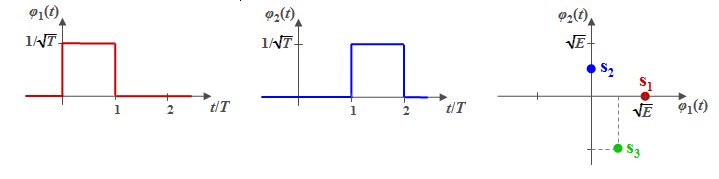
\includegraphics[width=0.7\textwidth]{../Mathematik_2/Bilder/dft_rechtecksignale_orthonormale_basis.png}
\end{center}
\end{itemize}
\end{exercisebox}

\begin{exercisebox}{Reelle und komplexe Fourierreihe}{ }
	Nehmen wir an, dass uns eine komplexe Fourierreihe f�r ein \(T\)-periodisches Signal \(f: \mathbb R \to \mathbb R, t\mapsto f(t)\) vorliegt, also
	\begin{equation}\label{FRC}  \mathrm{FR}_f(t) = \sum\limits_{k=-\infty}^{\infty}c_k\cdot e^{i k \omega_0\,t}\,.\end{equation}
	Bevor wir uns das im Detail anschauen, eine Vor�berlegung: offensichtlich gilt
	\begin{equation}\label{cplusk_cminusk}
		\forall k \in \mathbb N_0: \quad c_{-k} = \overline{c_{k}}\,,
	\end{equation}
	denn
\begin{eqnarray*}
	\forall k \in \mathbb N_0:\quad c_{-k} &=& \dfrac{1}{T}\int\limits_0^T f(t) \cdot e^{-i(-k) \omega_0\,t}\,\mathrm{d}t = \dfrac{1}{T}\int\limits_0^T f(t) \cdot e^{ik \omega_0\,t}\,\mathrm{d}t \\ &=& \dfrac{1}{T}\int\limits_0^T f(t) \cdot \overline{e^{-ik \omega_0\,t}}\,\mathrm{d}t = \overline{\dfrac{1}{T}\int\limits_0^T f(t) \cdot e^{-ik \omega_0\,t}\,\mathrm{d}t}\\ &=& \overline{c_{k}} \,.
\end{eqnarray*}
Jetzt zu der Fourierreihe. In der Reihe gibt es zu jedem \(k \geq 1\) zwei Frequenzanteile und zwar denjenigen mit der Amplitude \(c_k\) und denjenigen mit \(c_{-k}\). Diese beiden Summanden lassen sich zusammenziehen
	\begin{eqnarray*} c_{-k} \cdot e^{i (-k) \omega_0\, t}  + c_k \cdot e^{ik \omega_0\, t}  &=& c_{-k} \cdot \left( \cos( (-k) \omega_0 t) + i\, \sin( (-k) \omega_0 t)\right) + c_{k}\cdot \left( \cos( k \omega_0 t) + i\, \sin( k \omega_0 t)\right) \\
		&=& c_{-k} \cdot \left( \cos( k \omega_0 t) - i \,\sin( k \omega_0 t)\right) + c_{k}\cdot \left( \cos( k \omega_0 t) + i \sin( k \omega_0 t)\right) \\
		&=& \left( c_{-k} + c_k\right)\cdot \cos(k \omega_0 t) - i\,\left( c_{-k} - c_{k}\right)\cdot \sin(k\omega_0 t)  \\
		&\stackrel{\eqref{cplusk_cminusk}}{=}&  \left( \overline{c_{k}} + c_k\right)\cdot \cos(k \omega_0 t) - i\,\left( \overline{c_{k}} - c_{k}\right)\cdot \sin(k\omega_0 t)  \\
		&=&  \underbrace{2\, \mathrm{Re}(c_k)}_{\displaystyle{=a_k}}\cdot \cos(k \omega_0 t) + \underbrace{\left( -2\, \mathrm{Im}(c_k)\right)}_{\displaystyle{=b_k}}\cdot \sin(k\omega_0 t) \,.  \end{eqnarray*}
Die Zahlen \(a_k\) und \(b_k\) sind reell f�r \(k\geq 1\). Die Fusion von zwei komplexen Summanden f�hrt zu einer reellen Funktion, n�mlich einer harmonischen Schwingung bestehend aus einem (ungeraden) Sinusanteil und einem (geraden) Kosinusanteil zur selben Kreisfrequenz \(k\omega_0\).
Aus \eqref{cplusk_cminusk} folgt insbesondere, dass \(c_0 \in \mathbb R\) eine reelle Zahl ist und entsprechend der Formeln, die wir f�r \(k\geq 1\) gefunden haben, definieren wir
\[ 2 \cdot c_0 = a_0\,.\]
Damit lautet die �quivalente reelle Darstellung von \eqref{FRC}
\begin{equation}\label{FRR}
	\mathrm{FR}_f(t) = \dfrac{a_0}{2} + \sum\limits_{k=1}^\infty a_k \cdot \cos(k\omega_0\, t) + b_k \cdot \sin(k\omega_0\,t)\,,
\end{equation}
wobei die Formeln f�r die Umrechnung der Koeffizienten wie folgt lauten:
		\begin{eqnarray*}
			&& \begin{cases}
				a_0 =  2 \cdot c_0, \\[1ex]
				a_k = c_k + c_{-k} = 2\cdot \mathrm{Re}(c_k), \quad k\geq 1\\[1ex]
				b_k = i \cdot \left( c_k - c_{-k}\right) = -2 \cdot \mathrm{Im}(c_k) ,\quad k\geq 1 \,.
		\end{cases}
	\end{eqnarray*}
	M�chte man von der reellen Darstellung die komplexe ermitteln, dann gilt
		\begin{eqnarray*}
			&& \begin{cases}
				c_0 = \dfrac12\cdot a_0,\\[1ex]
				c_k = \dfrac12\cdot \left( a_k - i\, b_k\right) , \quad k\geq 1\,, \\[1ex]
			c_{-k} = \dfrac12\cdot \left( a_k + i \, b_k\right),\quad  , \quad k\geq 1\,. \end{cases}
	\end{eqnarray*}
\end{exercisebox}


\begin{exercisebox}[Matlab: Fourierpolynom Rechtecksignal als Funktion]

	\begin{itemize}
		\item[(a)]
	Das gegebene Rechtecksignal ist punktsymmetrisch zum Ursprung des Koordinatensystems. Die Fourierreihe enth�lt keinen Gleichstromanteil und auch keine geraden Anteile ( \(a_k=0, \; k\in \mathbb N_0\)):
	\[
		\mathrm{FR}_f(t) = \sum\limits_{n=1}^\infty b_n \cdot \sin\left( \dfrac{2\pi \, n}{T}\cdot  t\right) \,, \quad b_n= \dfrac{T}{2} \int\limits_{0}^T f(t) \cdot \sin\left( \dfrac{2\pi\, n}{T} \cdot t\right) \, \mathrm{d}t\,.
\]
F�hren wir die Integration zur Bestimmung der Koeffizienten \(b_n\) aus, so stellt sich raus, dass alle Koeffizienten mit geradem Index null werden, konkret:
\begin{eqnarray*}
	b_k = \dfrac{T}{2} \int\limits_{0}^T f(t) \cdot \sin\left( \dfrac{2\pi\, k}{T} \cdot t\right) \, \mathrm{d}t = \begin{cases} 0, \quad & k=2\cdot n\,, \\  \left( \dfrac{4\cdot A_0}{k\cdot \pi }\right), & k=2\cdot n+1\,. \end{cases}
\end{eqnarray*}
Die Fourierreihe f�r \(f\) lautet damit
	\[
		\mathrm{FR}_f(t) = \sum\limits_{n=0}^\infty \left( \dfrac{4\cdot A_0}{(2n+1)\cdot \pi }\right) \cdot \sin\left( \dfrac{2\pi \cdot (2n + 1)}{T}\cdot t \right) \,.
\]
		\item[(b)]
\end{itemize}

	\begin{minipage}{0.6\textwidth}
	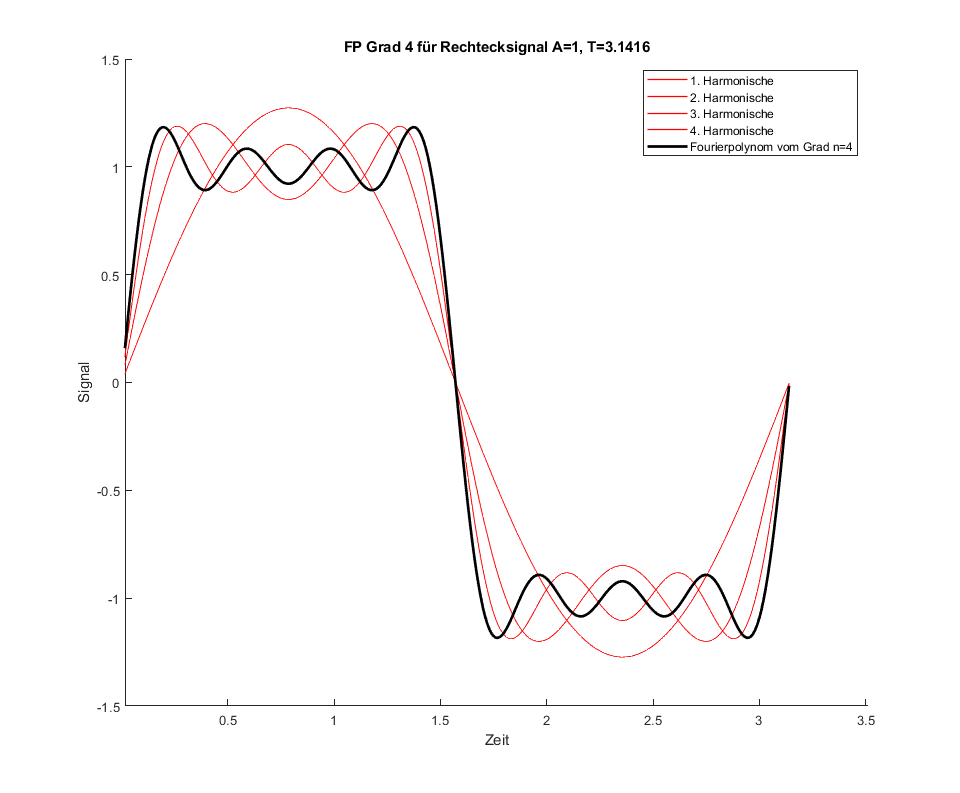
\includegraphics[width=\textwidth]{../Mathematik_2/Bilder/dft_rechtecksignal_fourierpolynom_grad_4.png}
\end{minipage}
	\begin{minipage}{0.3\textwidth}
\begin{lstlisting}
FourierSquare(1,pi,4)
\end{lstlisting}
\end{minipage}

	\begin{minipage}{0.6\textwidth}
	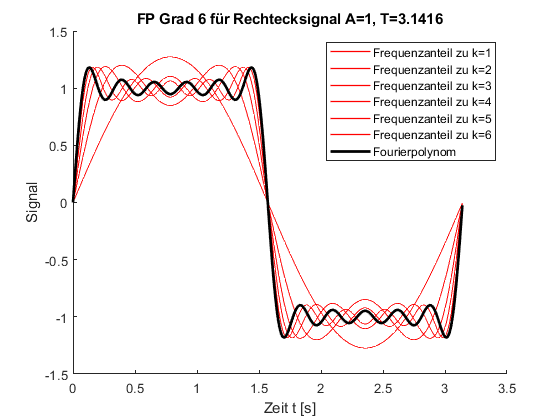
\includegraphics[width=\textwidth]{../Mathematik_2/Bilder/dft_rechtecksignal_fourierpolynom_grad_6.png}
\end{minipage}
	\begin{minipage}{0.3\textwidth}
\begin{lstlisting}
FourierSquare(1,pi,6)
\end{lstlisting}
\end{minipage}
\end{exercisebox}

\begin{exercisebox}[Minimierungsproblem]
	Die Koeffizienten \( a_0, a_1, \cdots, a_n \) und \(b_1, b_2, \cdots, b_n\) minimieren den Abstand zwischen \(f\) und \(g_n\), wobei der Abstand zwischen zwei belibiegen integrierbaren und \(2\pi\)-periodischen Funktionen wie folgt definiert ist:
	\[ ||f-g||_2 = \sqrt{\int\limits_{-\pi}^\pi |f(t)-g(t)|^2 \, \mathrm{d}t } \Leftrightarrow ||f-g||^2_2 = \int\limits_{-\pi}^\pi |f(t)-g(t)|^2 \, \mathrm{d}t \,. \]
	Setzen wir f�r \(g\) ein trigonometrisches Polynom ein, dann wird behauptet, dass das Fourierpolynom \(g_n\) sich von einem beliebigen \(g\) unterscheidet in sofern, dass es die Koeffizienten \(\left\{a_0, a_k,b_k, \, k=1,\cdots,n\right\} \) so eingestellt sind, dass \(\Phi\) minimiert wird. Eine notwendige Bedingung an die \(g_n\) ist also, dass alle folgenden partiellen Ableitungen verschwinden:
	\begin{equation}\label{partielle_Ableitungen_null}
		\begin{cases}
		\dfrac{\partial \Phi_n(f,g_n)}{\partial a_k} &= 0, \quad k=0,\cdots,n\,,\\
		\dfrac{\partial \Phi_n(f,g_n)}{\partial b_k} &= 0, \quad k=1,\cdots,n\,.
	\end{cases}
\end{equation}
Da wir die Funktion \(\Phi(f,g_n\) strukturell kennen, besteht die Hoffnung, dass wir die partiellen Ableitungen ausrechnen  und eine explizite Darstellung f�r die Koeffizienten ermitteln k�nnen, so dass \eqref{partielle_Ableitungen_null} erf�llt ist:
	\begin{eqnarray*} \Phi(f,g_n) = \| f-g_n\|^2_2 &=& \|g_n\|_2^2 +  \|f\|_2^2 - 2\langle g_n, f\rangle_2 \\ &=& \dfrac{\pi}{2} a_0^2 + \pi\sum\limits_{k=1}^n \left( a_k^2 + b_k^2\right)\\&& + \|f\|_2^2 - a_0 \langle 1, f\rangle - 2  \sum\limits_{k=1}^n \left( a_k \langle f, \cos(kx)\rangle + b_k \langle f, \sin(kx)\rangle \right) \\ &=& \Phi(a_0,\cdots,a_n,b_1,\cdots,b_n)\,.\end{eqnarray*}

F�hren wir die partiellen Ableitungen aus und setzen sie alle gleich null, dann erhalten wir Bestimmungsgleichungen f�r die unbekannten Koeffizienten!
\[
	\begin{array}{rcl c rcl r}
		\dfrac{\partial \Phi}{\partial a_0} &=& \pi a_0 - \langle 1, f\rangle = 0 & \Rightarrow & a_0 &=& \dfrac{1}{\pi}  \displaystyle{\int\limits_{-\pi}^\pi} f(x)\,\mathrm d x\,, & k=0\,,\\
		\dfrac{\partial \Phi}{\partial a_k} &=& 2\pi a_k - \langle \cos(kx), f\rangle = 0 & \Rightarrow & a_k &=& \dfrac{1}{\pi}  \displaystyle{\int\limits_{-\pi}^\pi} f(x) \cdot \cos(kx)\,\mathrm d x\,, &k\geq 1\,,\\
		\dfrac{\partial \Phi}{\partial b_k} &=& 2\pi b_k - \langle \sin(kx), f\rangle = 0 & \Rightarrow & b_k &=& \dfrac{1}{\pi}\displaystyle{ \int\limits_{-\pi}^\pi} f(x) \cdot \sin(kx)\,\mathrm d x\,,  &k\geq 1\,.
	\end{array}
\]
Was wir in dieser Aufgabe mit Hilfe von Differntialrechnung gezeigt haben, ist die Eigenschasft des Fourierpolynoms \(g_n\) die sogenannte Bestapproximation an die Funktion \(f\) im Vektorraum der trigonometrischen Polynome zu sein. Die Zerlegungskoeffizienten sind gerade die Projektionen auf das Orthonormalsystem der trigonometrischen Funktionen.
%
\end{exercisebox}

\begin{exercisebox}[Interpolationseigenschaft]
	Es ist also \[ \begin{cases} \tilde c_k = \sum\limits_{n=0}^{N-1} f_n\cdot e^{-i\,k\,n\,2\pi/N}\,\\ t_n & = n\cdot h = n\cdot T/N\,.\end{cases} \]
	Setzen wir \(t_n\) und danach \(\tilde c_k\) explizit in \(g_N\) ein:
\begin{eqnarray*}
	g_N(t_l) &=& \dfrac1N \cdot \sum\limits_{k=0}^{N-1} \tilde c_k\cdot e^{i\, k\, 2\pi/T \,t_l } \\[2ex]
	&=& \dfrac1N \cdot \sum\limits_{k=0}^{N-1} \textcolor{blue}{\tilde c_k}\cdot e^{i \,k \,l\,2\pi/N } \\[2ex]
	&=& \dfrac1N \cdot \sum\limits_{k=0}^{N-1}  \textcolor{blue}{\sum\limits_{n=0}^{N-1} f_n \cdot e^{-i \, k\,n\, 2\pi/N} } e^{i\, k \, l\, 2\pi/N } \\[2ex]
	&=& \dfrac{1}{N} \cdot \textcolor{blue}{\sum\limits_{n=0}^{N-1} f_n} \cdot \sum\limits_{k=0}^{N-1} \textcolor{blue}{ e^{-i \, k\,n\, 2\pi/N} }\cdot e^{i\, k \,l\, 2\pi/N } \\[2ex]
	&=& \dfrac{1}{N} \cdot \sum\limits_{n=0}^{N-1} f_l \cdot \sum\limits_{k=0}^{N-1} e^{i\, (l-n)\, k\,2\pi/N} \\[2ex]
	&\stackrel{(*)}{=}& \dfrac{1}{N} \sum\limits_{n=0}^{N-1} f_l \cdot \cdot N \cdot \delta_{ln} \\[2ex]
	&=& f_j\,.
\end{eqnarray*}
\((*)\) folgt aus der folgenden Beobachtung:
\[ \sum\limits_{k=0}^{N-1} e^{i \,(l-n)\, k \,2\pi/N} = \sum\limits_{k=0}^{N-1} \left( \left( W_N\right)^{l-n}\right)^k = N\cdot \delta_{ln} = \begin{cases} N,\quad l= n\,,\\ 0,\quad l\not=n\,, \end{cases} \]
	wobei sich das letzte Ergebnis im Detail wie folgt zeigen l��t
	\begin{itemize}
		\item f�r \(l=n\) wird der Exponent in jedem Summand null und damit \[\sum\limits_{k=0}^{N-1} W_N^{0\cdot k} = \sum\limits_{k=0}^{N-1} 1 = N\,.\]
		\item f�r \(l\not=n\) ist der Wert der Summe null. Summiert wird �ber eine beliebige \(N\).te Einheitswurzel \(Z:= \left( W_N\right)^{l-n}\). Der Wert der Summe ist bekannt und die \(N\).te Potenz einer Einheitswurzel ist eins:
			\[ \sum\limits_{k=0}^{N-1} Z^k = \dfrac{ Z^N -1}{Z -1} = \dfrac{1-1}{Z-1} = 0\,.\]
	\end{itemize}

	Das Ergebnis l��t sich wie folgt interpretieren: ob man ein diskretes Signal im Zeitbereich anschaut oder im Frequenzbereich ist egal - wie im kontinuierlichen Fall die Fouriertransformation, liegt im diskreten Fall ein Basiswechsel vor. Konkret: zur DFT gibt es eine inverse Abbildung, die dem diskreten Spektrum die Messwerte zuordnet. Man nennt diese Abbildung die inverse Diskrete Fouriertransformation [iDFT].
	\begin{eqnarray*}
		\textnormal{DFT:}\quad \{f_n\}_{n=0}^{N-1} &\mapsto& \{\tilde c_k\}_{k=0}^{N-1}\,, \\
		\tilde c_k &=& \sum\limits_{n=0}^{N-1} f_n\cdot e^{- i \, k\, n\, 2\pi/N}\,, \quad k=0,\cdots,N-1\,,\\
		\textnormal{iDFT:}\quad \{\tilde c_k\}_{k=0}^{N-1} &\mapsto& \{f_n\}_{n=0}^{n-1}\,, \\
		f_n &=& \dfrac{1}{N} \cdot \sum\limits_{k=0}^{N-1} \tilde c_k \cdot e^{i \, k\,n\, 2\pi/N}\,, \quad n=0,\cdots,N-1\,.
	\end{eqnarray*}
\end{exercisebox}

\begin{exercisebox}[DFT per Hand]
\begin{itemize}
\item[(a)] F�r $S_l=(t_l, f(t_l))$ gilt $S_1 = \left(0,8\right), S_2= \left(\frac14,4\right), S_3=\left( \frac12, 8\right), S_4=\left( \frac34,0\right)$
\item[(b)] Es gilt $\hat c_l = \displaystyle{ \sum\limits_{k=0}^3 e^{-i \,l\, \frac{2\pi}{n}  k} \cdot f(t_l) }$. Im vorliegenden Fall ist \(n=4\) und damit
	\begin{eqnarray*}
		\hat c_l = \displaystyle{ \sum\limits_{k=0}^3 e^{- i\,l \frac{2 \pi}{4} l} \cdot f(t_l) } \Rightarrow \left( \begin{array}{c} \hat c_0 \\\hat c_1 \\\hat c_2 \\ \hat c_3 \end{array}\right) = \left( \begin{array}{cccc} 1 & 1 & 1 & 1 \\ 1 & -i & -1 & i \\1 & -1 & 1 & -1 \\ 1 & i & -1 & -i \end{array}\right) \left( \begin{array}{c} 8 \\ 4 \\ 8 \\0\end{array}\right) \Rightarrow    \left( \begin{array}{c} \hat c_0 \\\hat c_1 \\\hat c_2 \\ \hat c_3 \end{array}\right) =\left( \begin{array}{c} 20 \\ -4i \\ 12  \\ 4i \end{array}\right)
	\end{eqnarray*}
\item[(c)] Die DFT liefert bis auf einen Skalierungsfaktor die Zerlegungskoeffizienten der harmonischen Schwingungen, die im Signal $f$ detektiert werden! Aus der DFT lassen sich die Samples zur�ckgewinnen durch die inverse, diskrete Fourier-Transformation (iDFT):
	\[ f_l = \frac{1}{n}\sum\limits_{k=0}^{n-1} \tilde c_k e^{i\, l\, \frac{2\pi}{n} k}\,. \]
\end{itemize}
\end{exercisebox}

\begin{exercisebox}{Matlab: Diskrete Fouriertransformation (DFT)}{ } % p.428 16.11 standard

	\begin{itemize}
		\item[(a)] Es gilt
			\begin{eqnarray*}
				n &=& 64\,,\\
				\Delta t &=& 0.01\,\mathrm{s}\,,\\
				T &=& n\cdot \Delta t\, \mathrm{s}\,,\\
				f_s &=& \dfrac{1}{\Delta t} = 100 \,\mathrm{Hz}\,,\\
				f_{\max} &=& \dfrac{f_s}{2} = 50\,\mathrm{Hz}\,,\\
				f_{\min} &=& \dfrac{1}{T} = 1.56\,\mathrm{Hz}\,,\\
			\end{eqnarray*}
			Die DFT detektiert die diskreten Frequenzen \(k\cdot f_{\min}\) f�r \(k=1,\cdots,\dfrac{n}{2} = 32\,.\) In dem gegebenen Signal gibt es genau zwei Frequenzanteile, die beide durch die DFT detektiert werden. Das Fourierpolynom, das durch die DFT definiert wird, interpoliert die Samples und reproduziert das Signal exakt.
		\item[(b)]
	\end{itemize}
	\begin{center}
		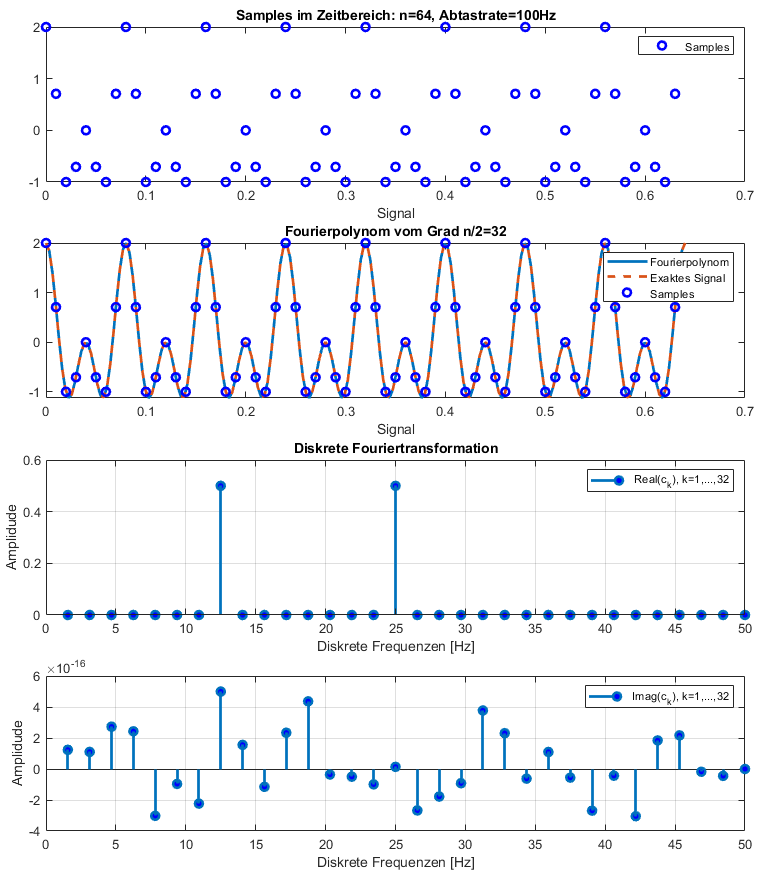
\includegraphics[width=\textwidth]{../Mathematik_2/Bilder/dft_signal_fourierpolynom_und_spektrum.png}
\end{center}
\end{exercisebox}

\begin{exercisebox}{Matlab: Experiment: DFT Leck-Effekt}{ } %

	\begin{itemize}
		\item[(a)] Das Signal \(f_1\) ist eine harmonische Schwingung mit Periode \(T_{\mathrm{min}}=1\). Im Zeitraum \([0,3)\) wird \(f_1\) mit \(n=8\) abgetastet. Wir erhalten:
		%\begin{enumerate}
		%	\item Die periodische Fortsetzung des Signals im Beobachtungsfenster \(f_1\big|_{[0,3)}\) ist genau \(f_1\) f�r alle \(t\geq 3\)!
		%	\item Die periodische Fortsetzung der \(8\) Samples, die im Intervall \([0,3)\) aufgezeichnet worden sind, liegen alle auf dem Graphen von \(f_1\) f�r \(t\geq 3\)!
		%\end{enumerate}
	\end{itemize}
\begin{center}
	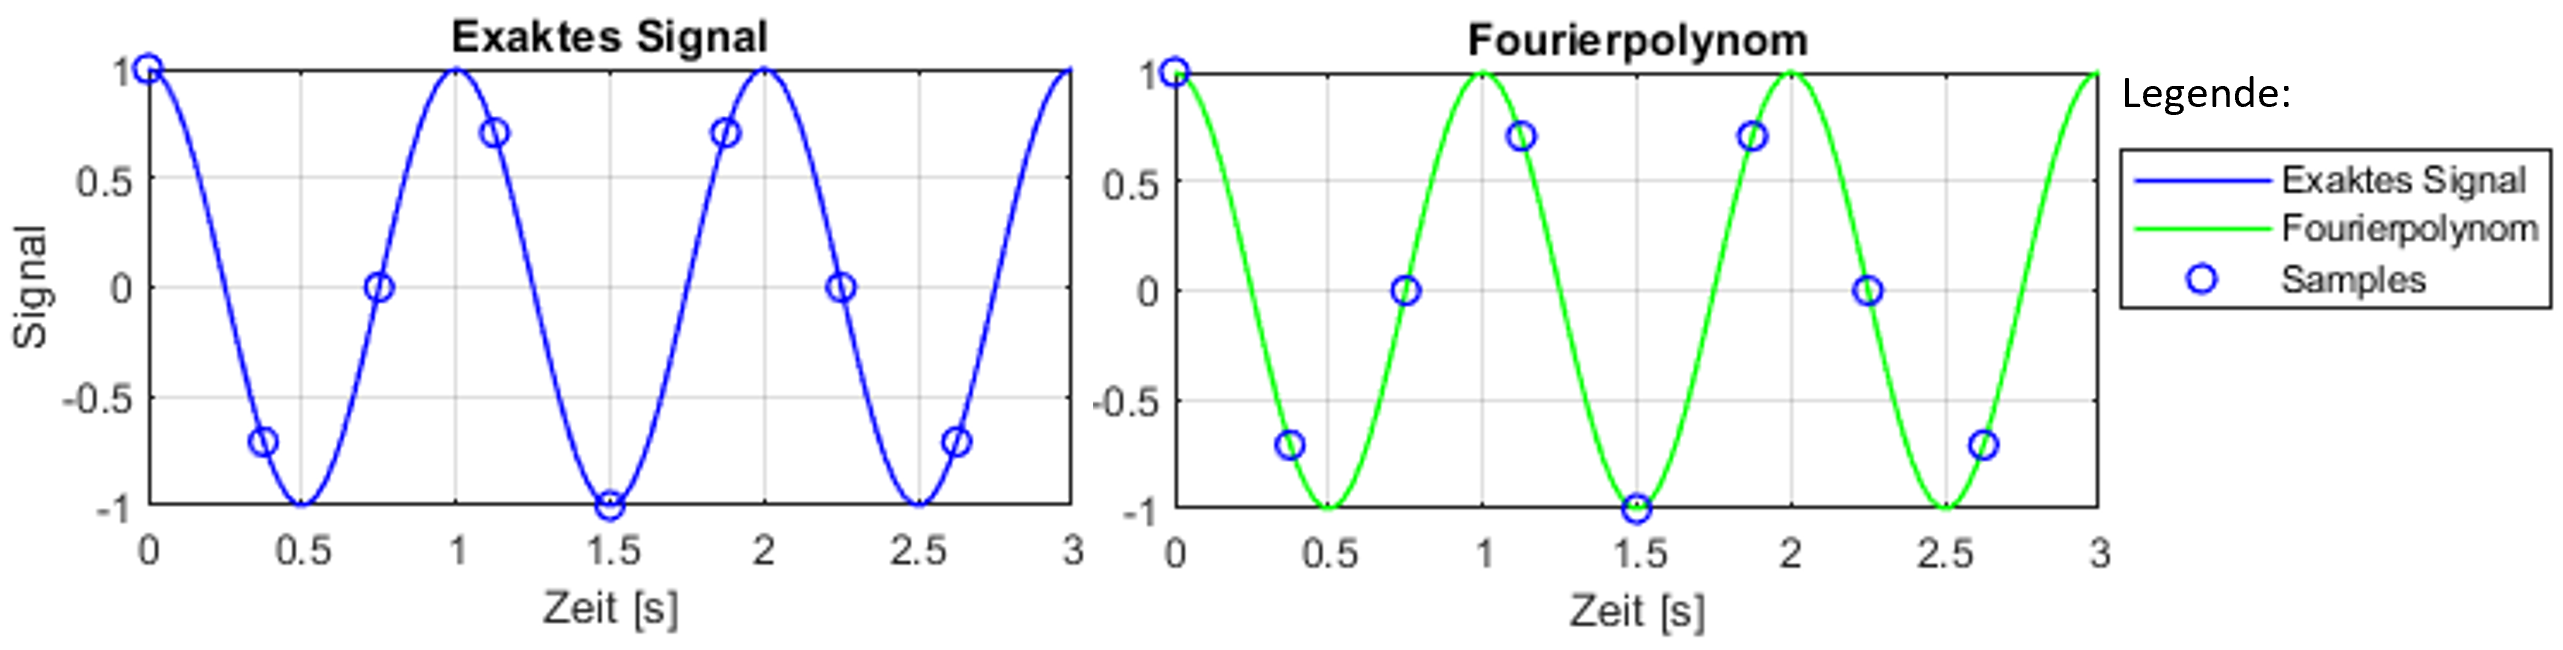
\includegraphics[width=\textwidth]{../Mathematik_2/Bilder/dft_interpolation_ganzzahlige_periodenzahl.png}
\end{center}
Links ist der Graph des exakten Signals mit den Interpolationspunkten gezeigt und rechts zus�tzlich das Fourierpolynom.

\begin{center}
	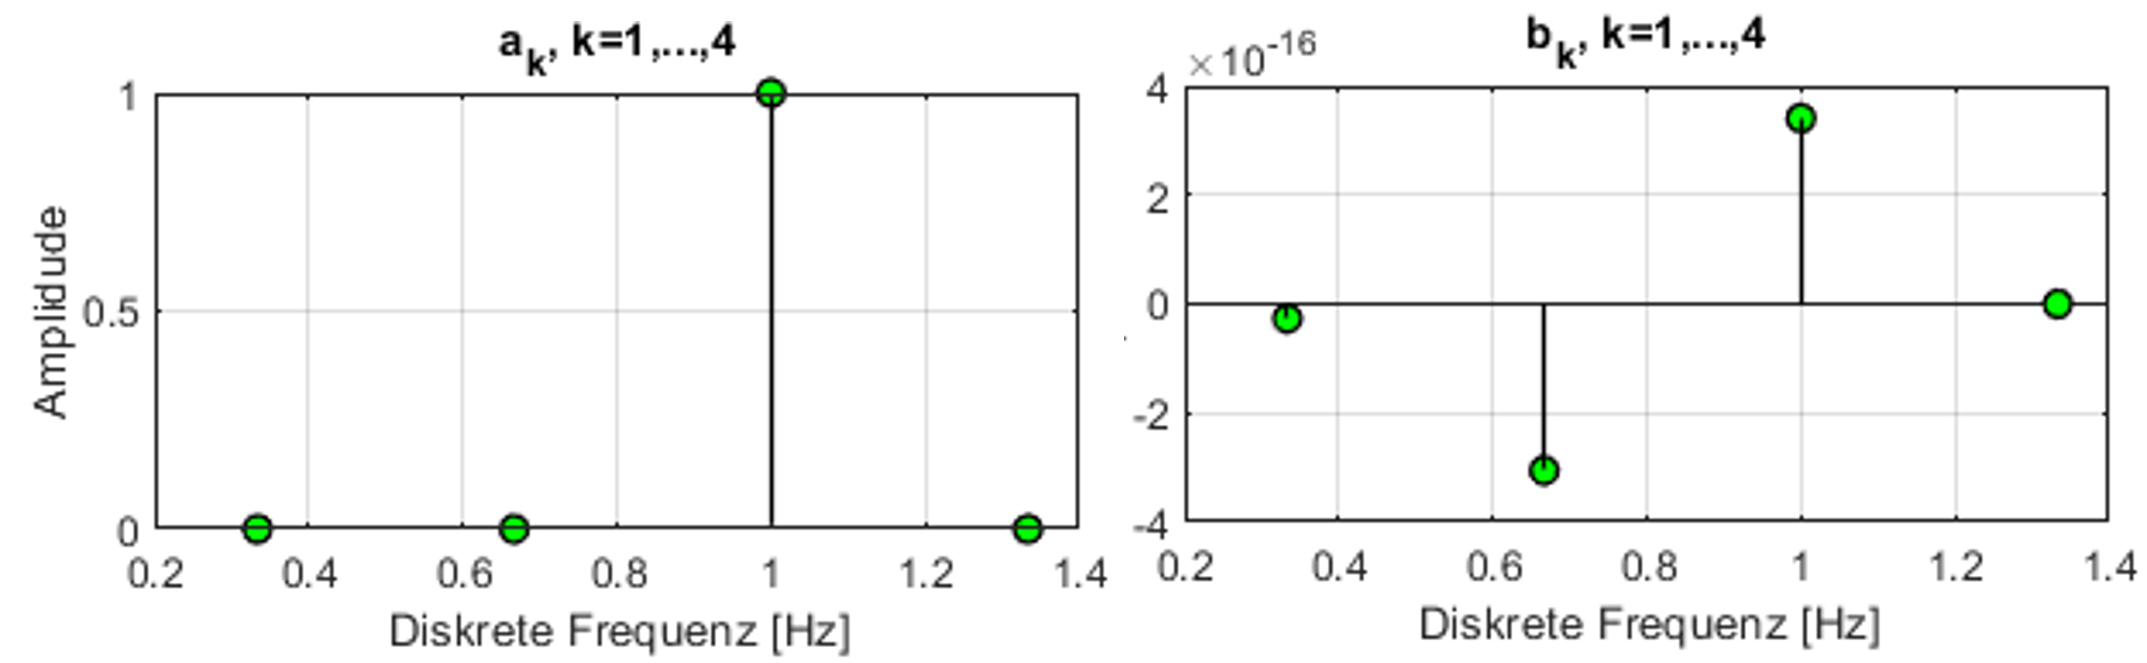
\includegraphics[width=0.8\textwidth]{../Mathematik_2/Bilder/dft_spektrum_ganzzahlige_periodenzahl.png}
\end{center}
Gezeigt ist das Spektrum, das die DFT liefert. Links die Ampliduden zu den geraden Anteilen und rechts die Ampliduden zu den ungeraden Anteilen.

\vspace{0.2cm}
Fazit:
\begin{itemize}
	\item Das Fourierpolynom interpoliert alle Samples.
	\item Es sind maximal \(4\) Frequenzen im Signal detektierbar.
	\item Von den \(8\) zugeh�rigen Amplituden ist nur \(a_3\not=0\). \(a_3\) entspricht der Amplitude der Grundschwingung.
	\item[\(\Rightarrow\)] Die eine Frequenz, die im Signal \(f_1\) vorhanden ist, wird durch die DFT detektiert.
	\item[\(\Rightarrow\)] Das Signal \(f_1\) wird durch das Fourierpolynom im Zeitbereich reproduziert (Fourier-Synthese).
\end{itemize}

\begin{itemize}
	\item[(b)] Das Signal \(f_2\) ist eine harmonische Schwingung mit Periode \(T_{\mathrm{min}} = \frac{6}{5}\). Im Zeitraum \([0,3)\) wird \(f_2\) mit \(N=8\) gesampelt. Wir erhalten:
		%\begin{itemize}
		%	\item Die periodische Fortsetzung des Signals im Beobachtungsfenster \(f_2\big|_{[0,3)}\) ist nicht \(f_2\) f�r alle \(t\geq 3\)!
		%	\item Die periodische Fortsetzung der \(8\) Samples, die im Intervall \([0,3)\) aufgezeichnet worden sind, liegen nicht auf dem Graphen von \(f_2\) f�r \(t\geq 3\)!
		%\end{itemize}
	\end{itemize}
	\begin{center}
	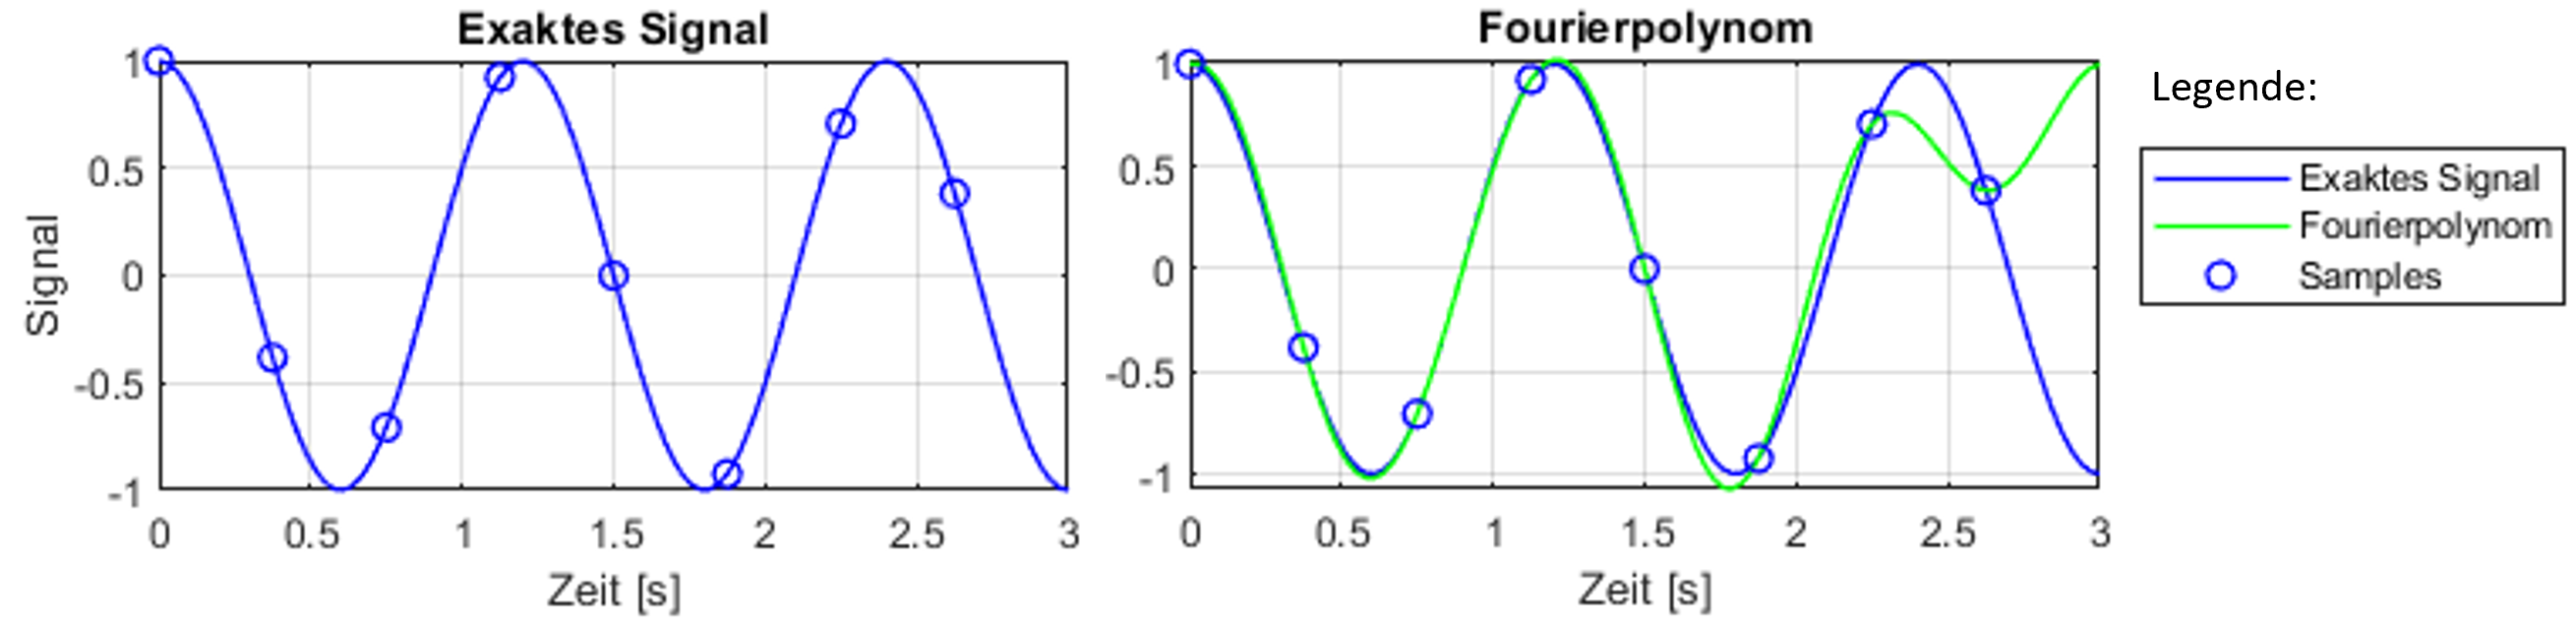
\includegraphics[width=\textwidth]{../Mathematik_2/Bilder/dft_interpolation_nichtganzzahlige_periodenzahl.png}
\end{center}
Links ist der Graph des exakten Signals mit den Interpolationspunkten gezeigt und rechts zus�tzlich das Fourierpolynom.
\begin{center}
	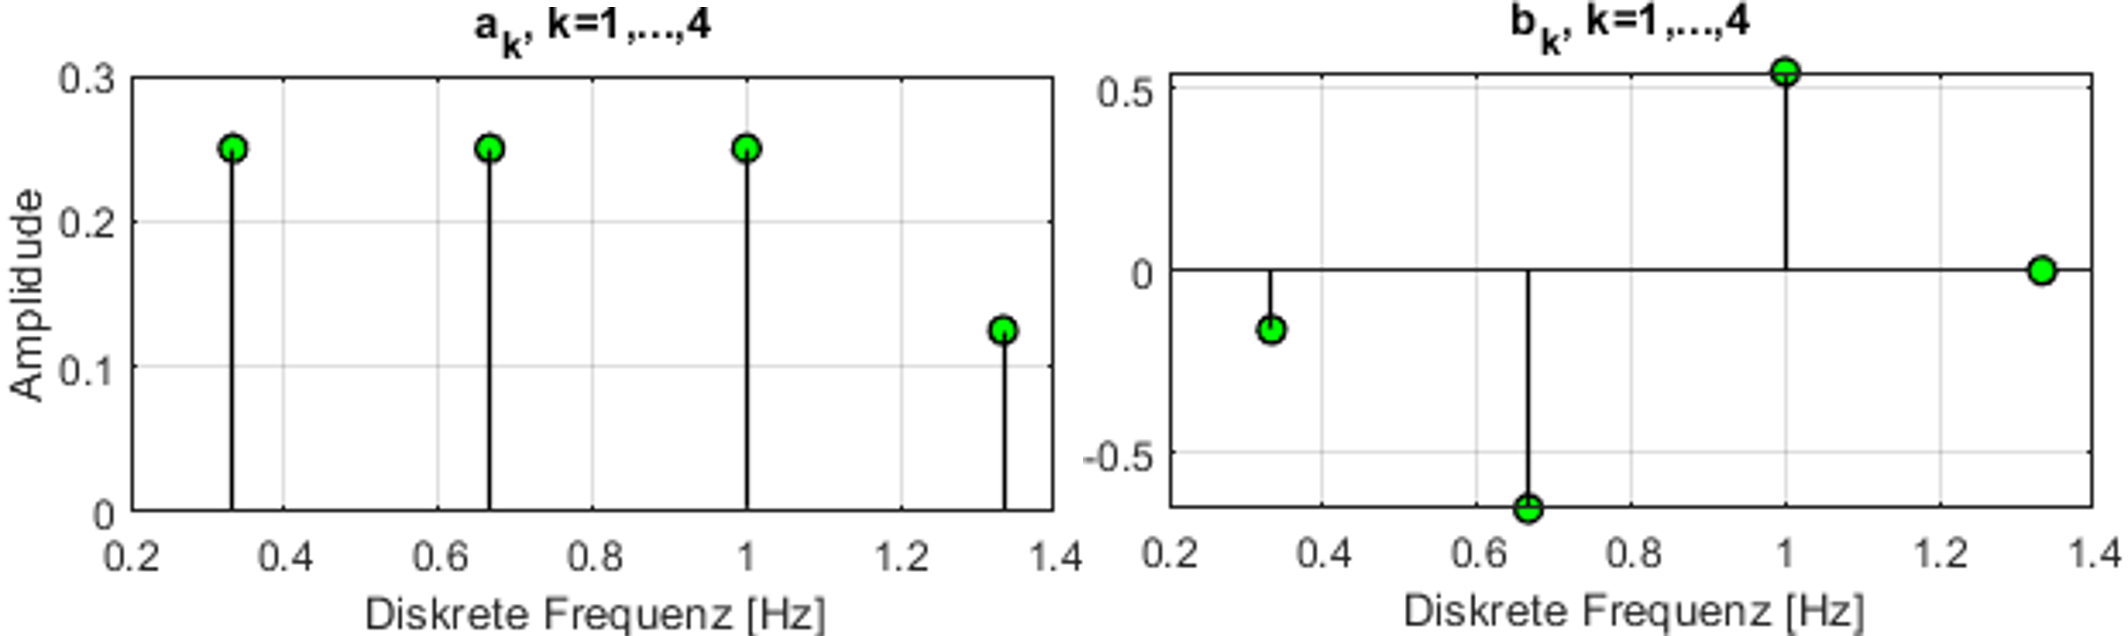
\includegraphics[width=0.8\textwidth]{../Mathematik_2/Bilder/dft_spektrum_nichtganzzahlige_periodenzahl.png}
\end{center}
Gezeigt ist das Spektrum, das die DFT liefert. Links die Ampliduden zu den geraden Anteilen und rechts die Ampliduden zu den ungeraden Anteilen.

\vspace{0.2cm}
Fazit:
\begin{itemize}
	\item Das Fourierpolynom interpoliert alle Samples.
	\item Es sind maximal \(4\) Frequenzen im Signal detektierbar.
	\item Alle \(8\) zugeh�rige Amplituden sind ungleich Null.
	\item[\(\Rightarrow\)] Die  Grundfrequenz, die im Signal \(f_2\) vorhanden ist, wird durch die DFT \textbf{nicht} detektiert.
	\item[\(\Rightarrow\)] Das Signal \(f_2\) wird \textbf{nicht} reproduziert.
\end{itemize}


\noindent{ (c)} Warum es dazu kommt, dass die DFT in (a) das Signal \(f_1\) exakt reproduziert, ist recht einfach zu sehen: das Beobachtungsintervall \([0,3)\) ist ein ganzzahliges Vielfaches der minimalen Periode \(T_{\mathrm{min}}=1\) des Signals \(f_1\) und das hei�t, dass die DFT das Spektrum von \(f_1\) berechnet, weil die \textcolor{blue}{periodischen Fortsetzung} von \(f_1\big|_{ [0,3)} \) \textbf{identisch} mit \(f_1\) ist:
\vspace{0.2cm}
	\begin{center}
		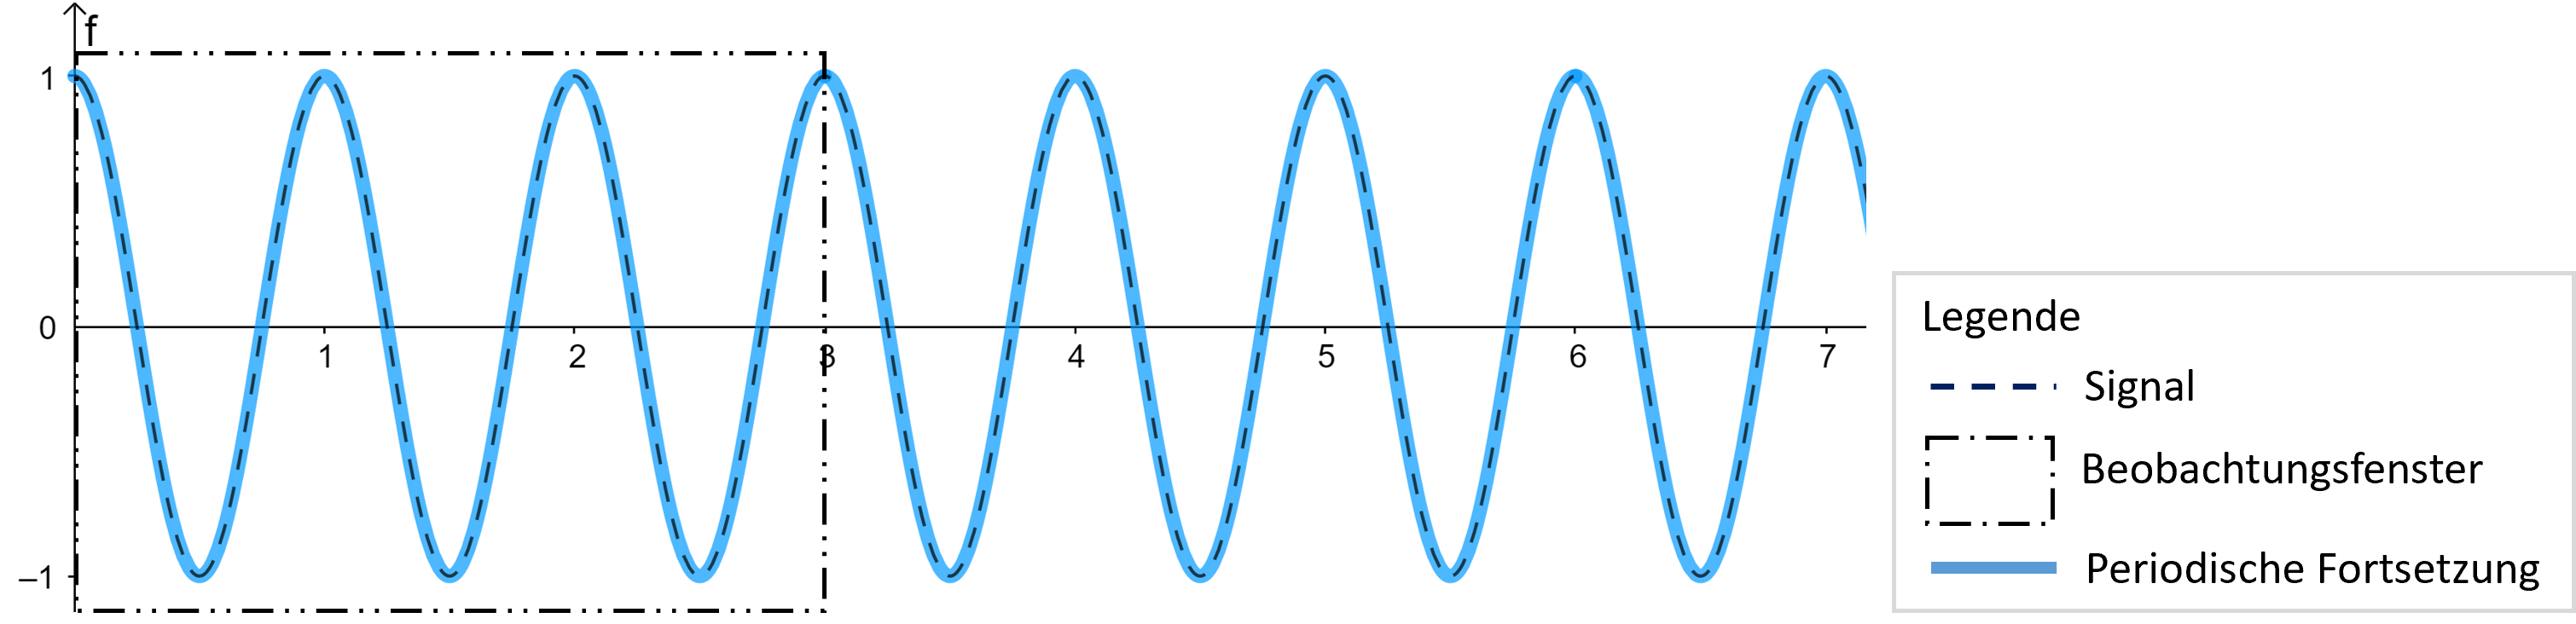
\includegraphics[width=0.9\textwidth]{../Mathematik_2/Bilder/dft_periodische_fortsetzung_ganzzahlige_periodenzahl.png}
\end{center}

%Die Fouriertransformierte im stetigen Frequenzraum ist die Superposition zweier Delta-Impulse, wobei \(2\pi\) und die andere in \(-2\pi\) lokalisiert ist:
%\[ f_1 \laplace \dfrac{\sqrt{2\pi}}{2} \left( \delta_{2\pi} + \delta_{-2\pi}\right)\,. \]
%	\begin{eqnarray*}
%		f_1(t) &=& \dfrac{1}{2\pi} \int\limits_{-\infty}^\infty \dfrac{\sqrt{2\pi}}{2} \left( \delta_{2\pi} + \delta_{-2\pi} \right) \cdot e^{i\omega\,t} \, \mathrm{d}\omega  \\
%				&=& \dfrac{1}{2}  \left( e^{i \, 2\pi \, t} + e^{-i\,2\pi \,t}\right) = \cos(2\pi\,t)\,.
%		\end{eqnarray*}
\vspace{0.2cm}

Genau das �ndert sich in (b): das Beobachtungsintervall \([0,3)\) ist kein Vielfaches der minimalen Periode \(T_{\mathrm{min}} = \frac65 \) von \(f_2\) und das hei�t, dass die DFT gar nicht das Spektrum von \(f_2\) diskretisiert! Die periodische Fortsetzung von \(f_2\big|_{ [0,3)} \) stimmt n�mlich \textbf{nicht} mit \(f_2\) �berein:
\vspace{0.2cm}
	\begin{center}
		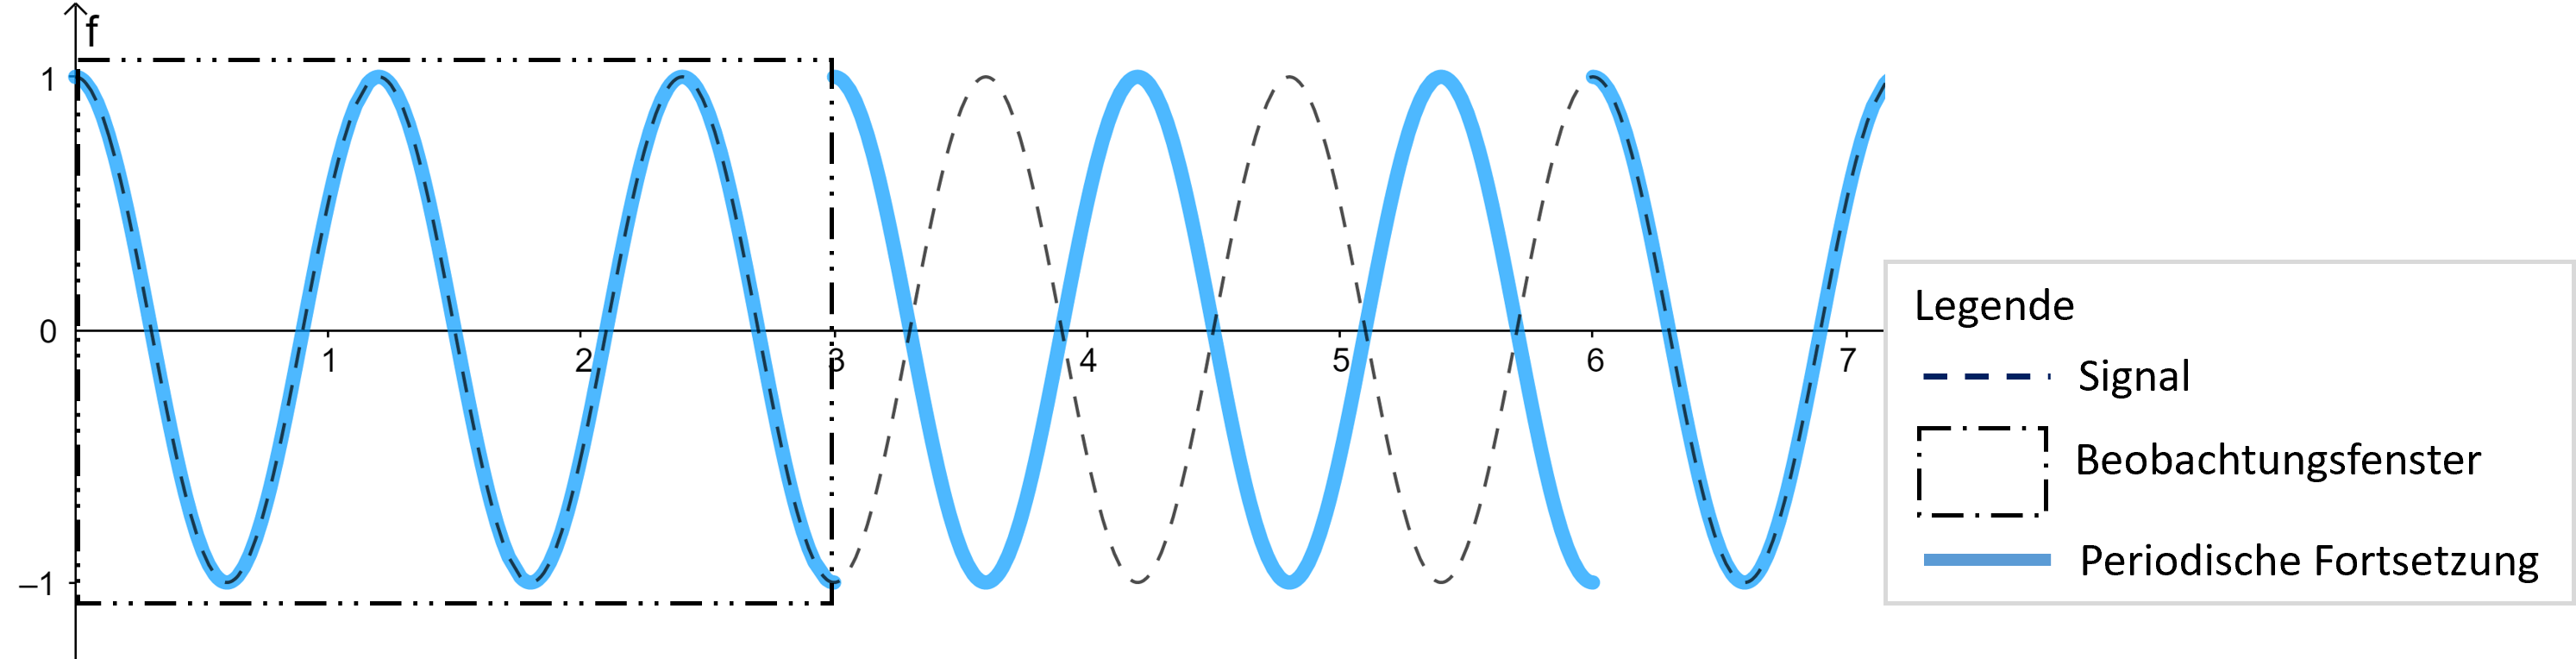
\includegraphics[width=0.9\textwidth]{../Mathematik_2/Bilder/dft_periodische_fortsetzung_nichtganzzahlige_periodenzahl.png}
\end{center}

\vspace{0.2cm}
Offensichtlich ist die \textcolor{blue}{periodische Fortsetzung}, die der DFT zu Grunde liegt, keine harmonische Schwingung mehr! Und das hei�t
			\begin{itemize}
				\item[\(\Rightarrow\)] Ihr Spektrum kann nicht mehr nur aus einem Beitrag bestehen.
				\item[\(\Rightarrow\)] Das Fourierpolynom, das durch die DFT erzeugt wird, kann das Ausgangssignal \(f_2\) nicht reproduzieren.
			\end{itemize}

			\textbf{Trotzallem ist die DFT aussagekr�ftig, wenn man versteht, wie sie zu lesen ist} und das schauen wir uns jetzt in einem allgemeinen Setting an. Let's go.

			Allgemein gilt: das Spektrum eines nicht periodischen, absolut integrierbaren Signals \(f_r\) wird durch dessen Fouriertransformierte \(\hat f_r\) beschrieben. \(\hat f_r\) ist die Fouriertransformierte von \(f_r\), also
			\[ f_r: t \mapsto g(t)  \quad  \stackrel{\displaystyle{ \mathcal F}}{\longrightarrow} \quad  \hat {f_r}: \omega \mapsto \dfrac{1}{\sqrt{2\pi}}\int\limits_{-\infty}^\infty f_r(t) \cdot e^{-i\,\omega \, t}\, \mathrm{d}t\,.\]
			Betrachten wir als Beispiel f�r \(f_r\) das folgende Signal
			\[ f_r: t\mapsto \begin{cases} A \cos(\omega_0\, t), &\quad  -1 \leq t < 1 \,,\\0, &\quad \mathrm{sonst}\,.\end{cases}  \]
			\(f_r\) schneidet also aus der harmonischen Schwingung \(f: t\mapsto A\cdot \cos(\omega_0\,t)\) das Intervall \([-1,1]\) aus und setzt links von \(-1\) und rechts von \(1\) mit null fort. Die Fouriertransformierte von \(f_r\) lautet:
\begin{eqnarray}
	\hat f_r(\omega) &=& \dfrac{1}{\sqrt{2\pi}}\int\limits_{-\infty}^\infty f_r(t)\cdot  e^{- i\omega\,t } \,\mathrm{d}t  \stackrel{(*)}{=} \dfrac{2}{\sqrt{2\pi}}\int\limits_{0}^{1} A\cdot \cos(\omega_0\, t) \cdot  \cos(\omega\,t) \,\mathrm{d}t  \nonumber\\
	& \stackrel{\eqref{int_cosat_cosbt}}{=}& \dfrac{A}{\sqrt{2\pi}} \cdot \left(\dfrac{\sin\left( \omega_0 -\omega\right)}{\omega_0-\omega} + \dfrac{\sin\left( \omega_0+\omega\right)}{\omega_0 + \omega} \right)\,. \label{hat_f_r}
			\end{eqnarray}
			wobei
			\begin{itemize}
				\item in \( (*)\) ausgenutzt wird, dass \(f_r\) eine gerade Funktion ist,
				\item in \eqref{int_cosat_cosbt} die folgende Stammfunktion benutzt worden ist
			\begin{equation}\label{int_cosat_cosbt}
				\int \cos(a\, t) \cdot  \cos(b\,t) \,\mathrm{d}t = \frac12 \left( \dfrac{\sin\left( (a-b)\,t\right)}{a-b} + \dfrac{\sin\left( (a+b) \, t\right)}{a+b} \right)
				      \end{equation}
		      \end{itemize}
		      Nehmen wir nun an, wir tasten das Signal \(f_r\) auf dem Intervall \([-1,1)\) mit \(n\) Samples ab und benutzen diese Samples f�r eine DFT. Die DFT sind, bis auf einen Skalierungsfaktor, die Funktionswerte von \(\hat f_r\) an den Kreisfrequenzen, die die DFT detektiert werden k�nnen, also an den diskreten Stellen \[ \omega = \dfrac{2\pi}{t_N}\cdot k\,, \quad k=-\dfrac{N}{2},\cdots,\dfrac{N}{2}\,,\]
		      Also folgt konkret
		      \begin{eqnarray} c_k &=& \dfrac{\sqrt{2\pi}}{2}\cdot \hat f_r\left( \dfrac{ 2\pi}{T}\cdot k\right) \label{dft_fr}\\
		&=& \dfrac{ A}{2}\cdot\left(  \dfrac{\sin\left(\dfrac{ 2\pi}{\textcolor{blue}{t_N}}\cdot k -\textcolor{red}{\omega_0}\right)}{\dfrac{ 2\pi}{\textcolor{blue}{t_N}}\cdot k -\textcolor{red}{\omega_0}} +   \dfrac{\sin\left(\dfrac{ 2\pi}{\textcolor{blue}{t_N}}\cdot k +\textcolor{red}{\omega_0}\right)}{\dfrac{ 2\pi}{\textcolor{blue}{t_N}}\cdot k +\textcolor{red}{\omega_0}}\right)\,, \quad k=-\dfrac{N}{2},\cdots,\dfrac{N}{2}\,. \nonumber
\end{eqnarray}
Jetzt ist es wichtig die Bedeutung der blau und rot eingeb�rbten Terme zu kennen:
		      \begin{itemize}
			      \item \( \textcolor{blue}{t_N} \) ist die Zeitspanne, die Breite des Beobachtungsfensters.\footnote{ \(t_N\) ist die Periode, von der die DFT ausgeht. }
			      \item \(\textcolor{red}{\omega_0}\) ist die Grundfrequenz des Signals \(f\). Es gilt \(\textcolor{red}{T_{\mathrm{min}} = \dfrac{2\pi}{\omega_0} }\).
		      \end{itemize}

		      \vspace{0.2cm}

		      Grunds�tzlich k�nnen zwei verschiedene F�lle auftreten. Wir machen zwei Beispiele. Das erste Beispiel verdeutlicht die Ergebnisse aus Aufgabenteil (a) und das zweite Beispiel pr�zisiert und erkl�rt die Ergebnisse aus Aufgabenteil (b).

		      \vspace{0.2cm}
		      \noindent\textbf{Beispiel (a)} Betrachte \(f_r\) auf \([-1,1)\) mit \(A=1\) und \(\omega_0 = 2\pi\), also
		      \begin{itemize}
			      \item Beobachtungsfenster \([-1,1)  \Rightarrow \textcolor{blue}{ t_N = 2 }  \Rightarrow \) Kreisfrequenzen DFT \( \textcolor{blue}{\dfrac{2\pi}{t_N}\cdot k = \pi\cdot k}\,.\)
			      \item Grundfrequenz \(\textcolor{red}{\omega_0=2\pi \; \Rightarrow \; T = 1 }\).
		      \end{itemize}

		      Das Signal ist im folgenden Bild dargestellt und zwar links im Zeitbereich \(f_r: t\mapsto f_r(t)\) und rechts im Frequenzbereich \(\hat f_r: \omega\mapsto \hat {f_r}(\omega)\):
		      \begin{center}

			      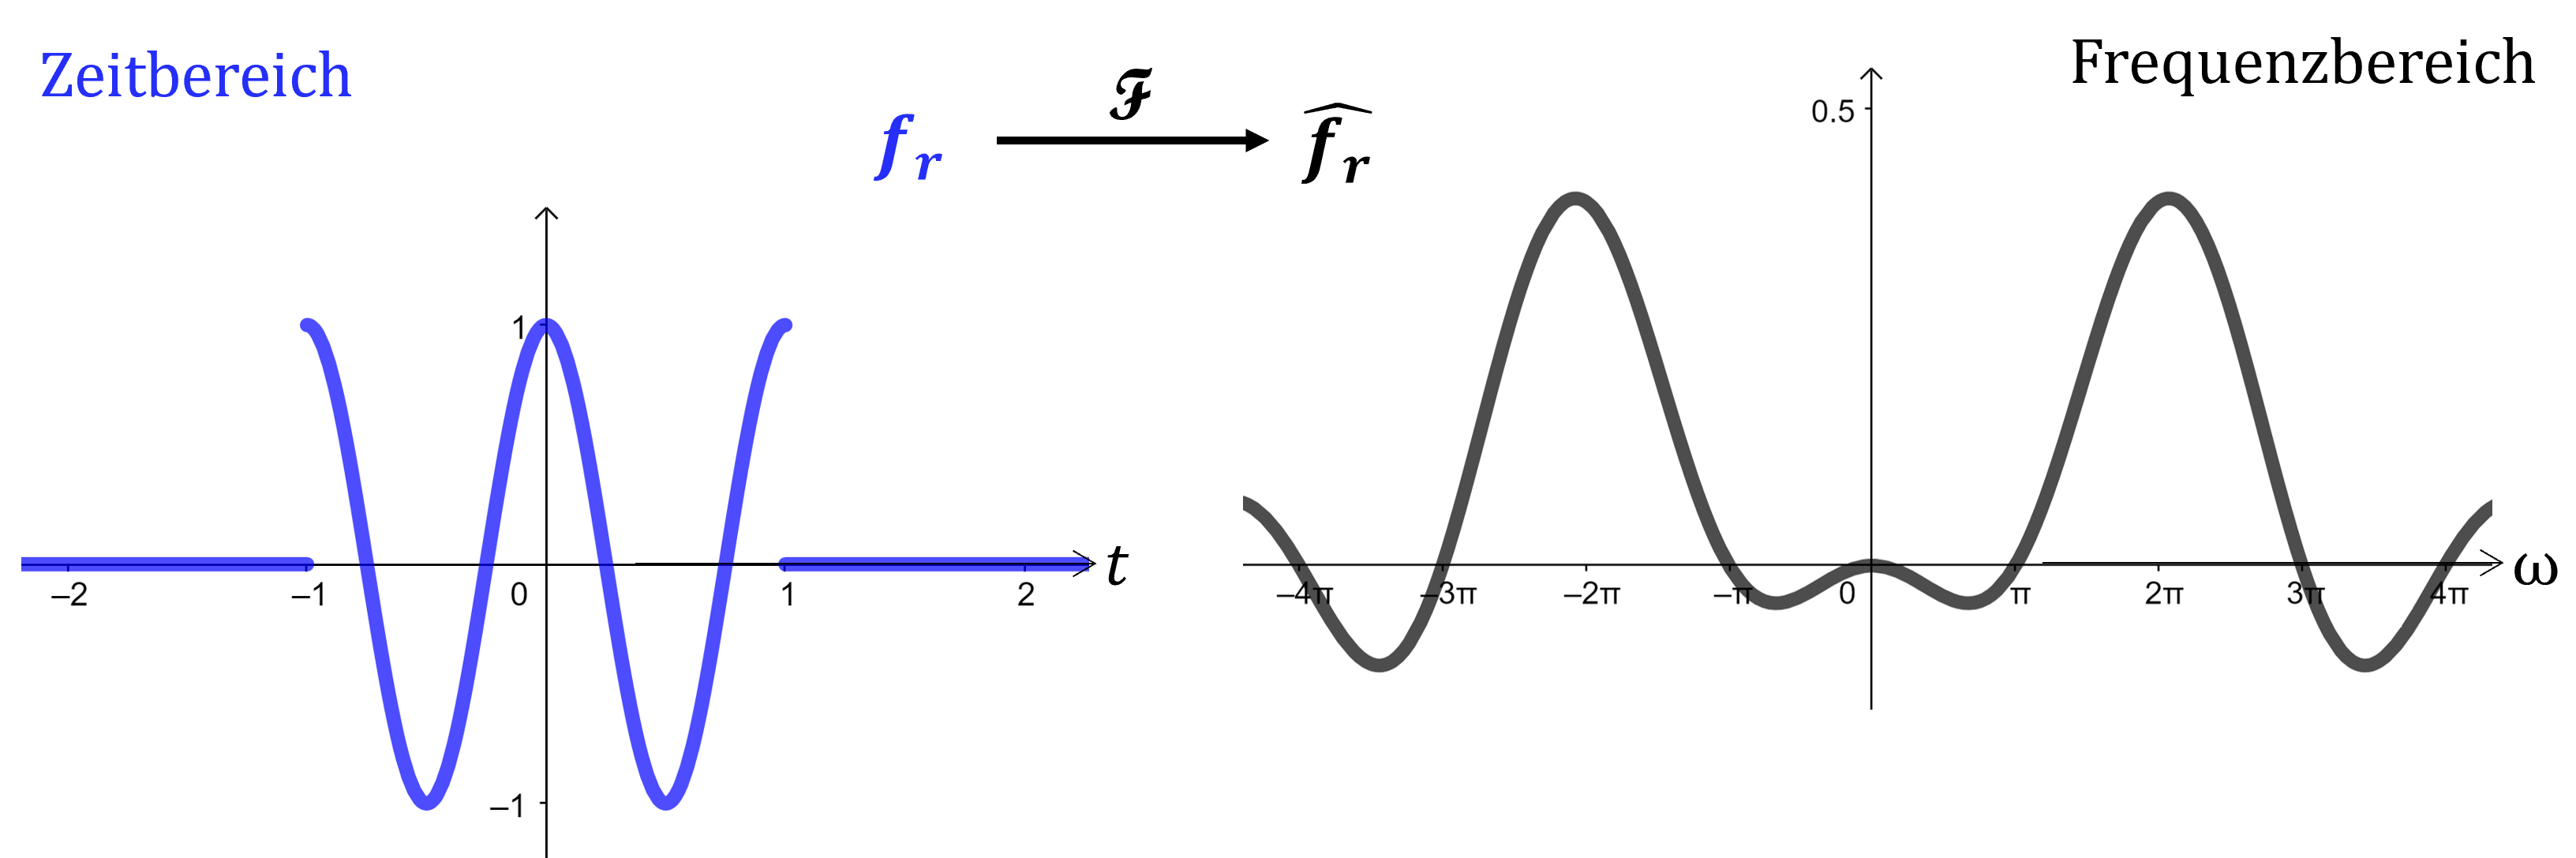
\includegraphics[width=0.8\textwidth]{../Mathematik_2/Bilder/fouriertransformation_kosinus_endliches_beobachtungsfenster.png}
\end{center}

Die DFT ist nach \eqref{dft_fr} die Diskretisierung des Spektrums \(\hat {f_r}\) an den Stellen \(\omega = \pi\cdot k\) f�r \(k= -\dfrac{n}{2},\cdots,\dfrac{n}{2}\) und da wir \(\hat {f_r}\) kennen, k�nnen wir uns die genau anschauen:
\begin{eqnarray*} c_k &=&  \dfrac{A}{2}\cdot\left(  \dfrac{\sin\left(\textcolor{blue}{\pi\cdot k} -\textcolor{red}{2\pi}\right)}{\textcolor{blue}{\pi\cdot k} -\textcolor{red}{2\pi}} + \dfrac{\sin\left(\textcolor{blue}{\pi\cdot k} + \textcolor{red}{2\pi}\right)}{\textcolor{blue}{\pi\cdot k} + \textcolor{red}{2\pi}}\right)\,, \quad k=-\dfrac{n}{2},\cdots,\dfrac{n}{2}\,, \\
	&=& \begin{cases} \dfrac{A}{2}\,,\quad |k|=2\,, \quad (\textnormal{Regel von L'Hospital})\,,\\ 0\,,\quad \textnormal{sonst}\end{cases}
	\end{eqnarray*}
		      \begin{center}
			      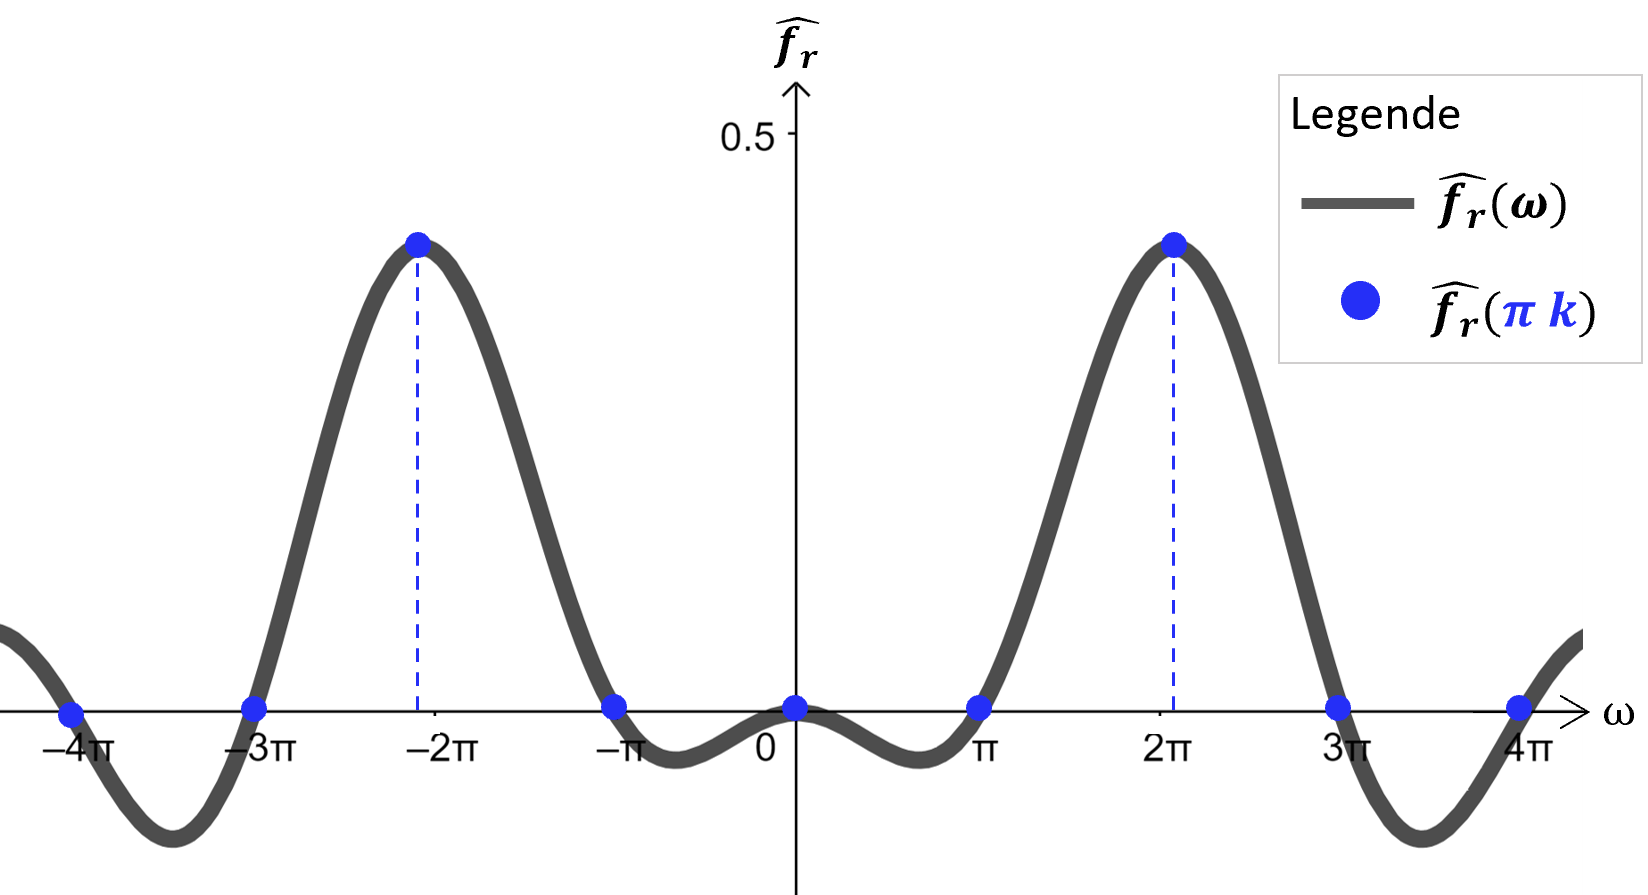
\includegraphics[width=0.7\textwidth]{../Mathematik_2/Bilder/dft_frequenzraster_auf_spektralmaxima.png}
\end{center}

	Die Grundfrequenz von \(f\) wird durch die DFT f�r \(|k|=2\) identifiziert und alle anderen \(c_k\) fallen genau auf Nullstellen der Funktion \(\hat f_r\)! Die Fourier-Synthese reproduziert \(f\):
	\[ g_n(t) = c_{-2}\, e^{-i\,2\pi\,t} + c_2\, e^{i\,2\pi,t} = A \cdot \cos(2\pi\,t) = f(t)\,.\]

	Entscheidend ist die Wahl des Beobachtungsfensters: immer wenn das Beobachtungsfenster, das der DFT zu Grunde liegt, ein ganzzahliges Vielfaches der Periode \(T_{\mathrm{min}}\) von \(f\) ist, also
	\[ T = m\cdot T_{\mathrm{min}}\,, \]
	dann wird die Grundfrequenz von \(f\) durch die DFT exakt detektiert!

	\vspace{0.2cm}

	\noindent\textbf{Beispiel (b)} Betrachte \(f_r\) mit \(A=1\) und \(\omega_0 = \frac65\pi\), also
		      \begin{itemize}
			      \item Beobachtungsfenster \([-1,1) \; \Rightarrow \textcolor{blue}{ t_N = 2 } \; \Rightarrow \) Kreisfrequenzen DFT \( \textcolor{blue}{\dfrac{2\pi}{t_N}\cdot k = \pi\cdot k}\,.\)
			      \item Grundfrequenz \(\textcolor{red}{\omega_0=\frac65 \pi} \; \Rightarrow \; T_{\mathrm min} = 1.2\).
		      \end{itemize}

	Das Signal ist im folgenden Bild dargestellt und zwar links im Zeitbereich \(f_r: t\mapsto f_r(t)\) und rechts im Frequenzbereich \(\hat f_r: \omega\mapsto \hat {f_r}(\omega)\):
		      \begin{center}
			      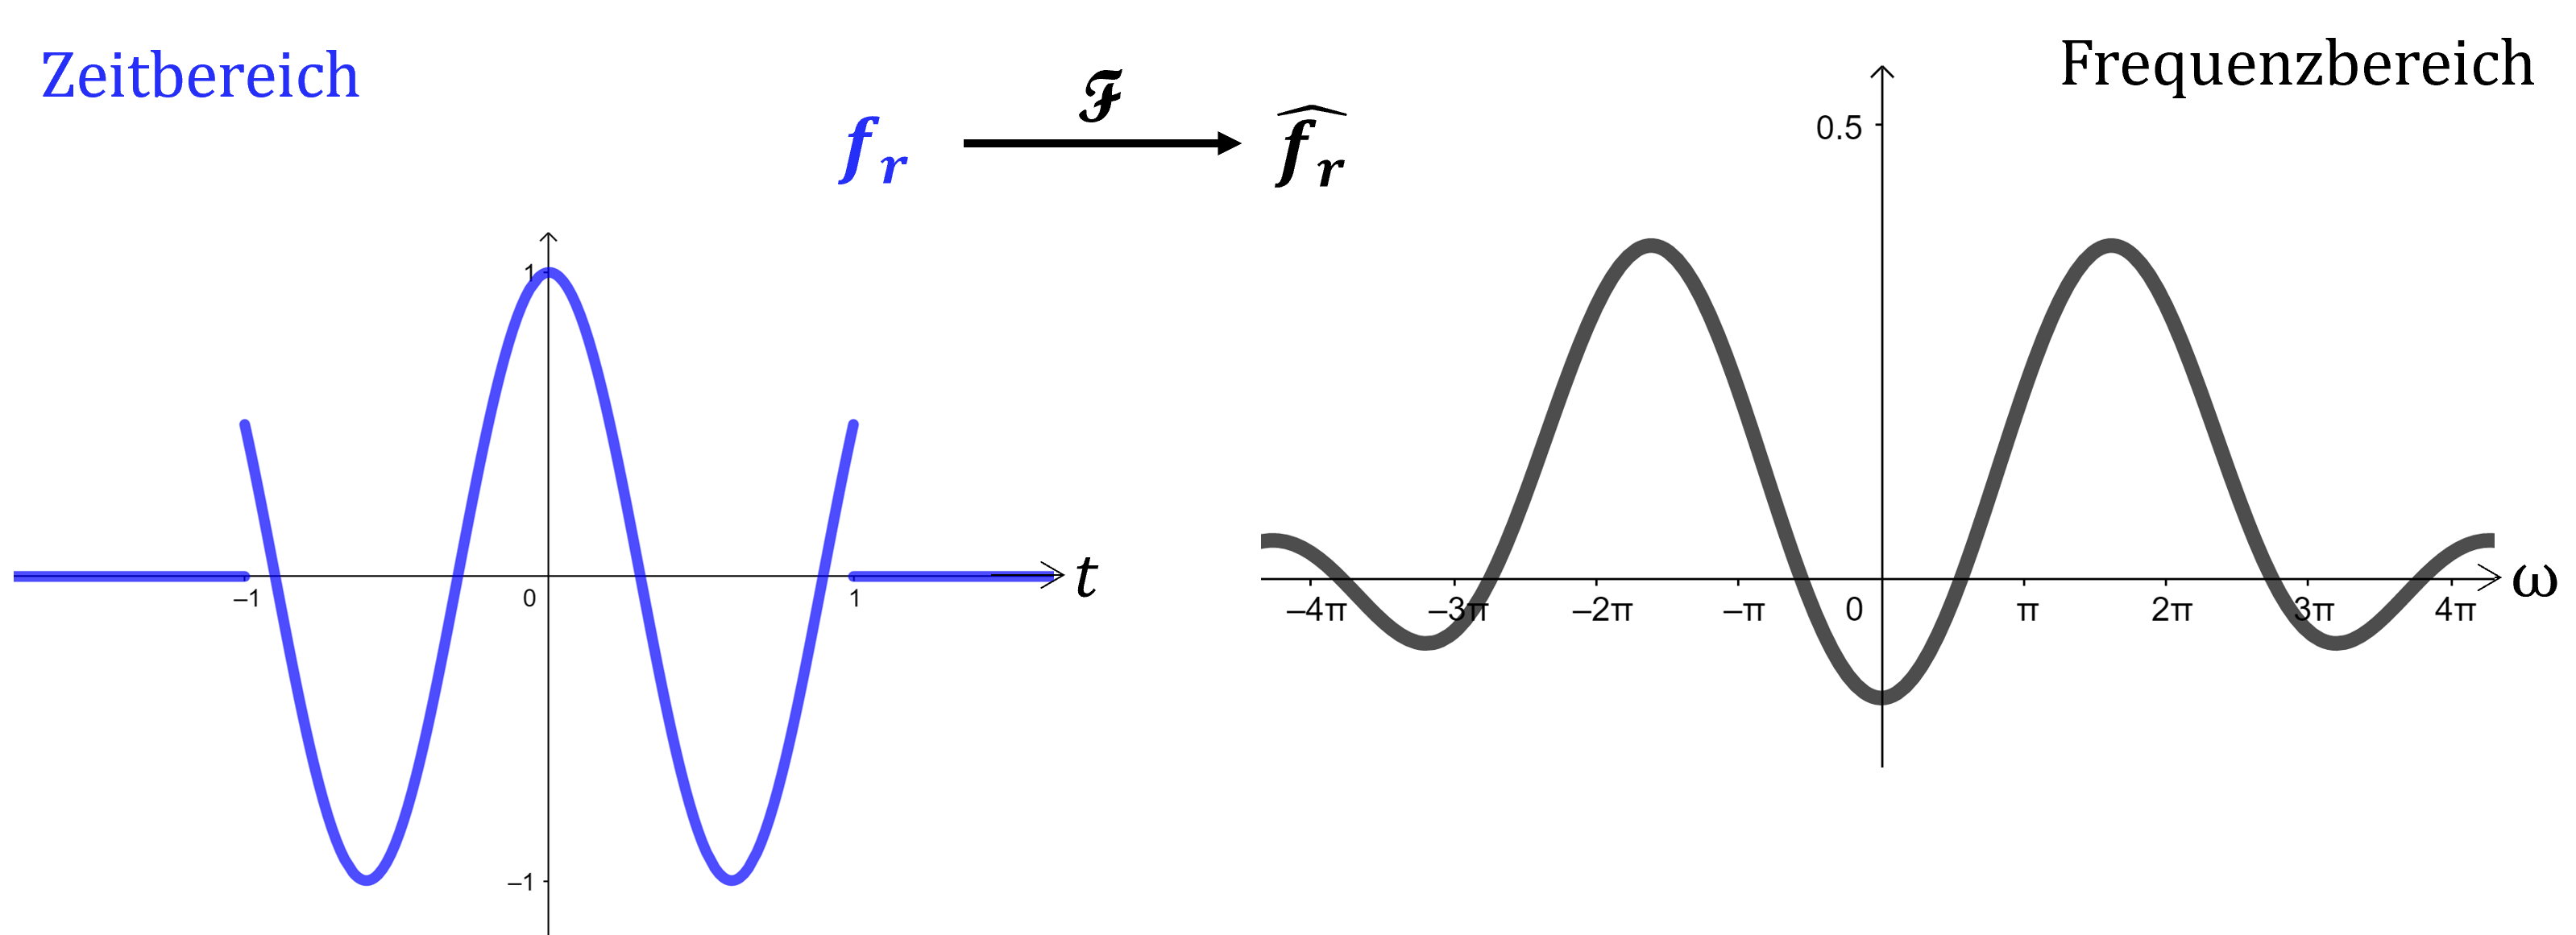
\includegraphics[width=0.8\textwidth]{../Mathematik_2/Bilder/fouriertransformation_sinus_endliches_beobachtungsfenster.png}
\end{center}
Die DFT ist nach \eqref{dft_fr} die Diskretisierung des Spektrums \(\hat {f_r}\) an den Stellen \(\omega = \pi\cdot k\) f�r \(k= -\dfrac{N}{2},\cdots,\dfrac{N}{2}\) und da wir \(\hat {f_r}\) kennen, k�nnen wir uns die genau anschauen:
\begin{eqnarray*} c_k =  A\cdot\left(  \dfrac{\sin\left(\textcolor{blue}{\pi\cdot k} -\textcolor{red}{\frac65\pi}\right)}{\textcolor{blue}{\pi\cdot k} -\textcolor{red}{\frac65\pi}} +   \dfrac{\sin\left(\textcolor{blue}{\pi\cdot k} + \textcolor{red}{\frac65\pi}\right)}{\textcolor{blue}{\pi\cdot k} + \textcolor{red}{\frac65\pi}}\right)  \not = 0 \,, \quad k=-\dfrac{N}{2},\cdots,\dfrac{N}{2}\,.
	\end{eqnarray*}
		      \begin{center}
			      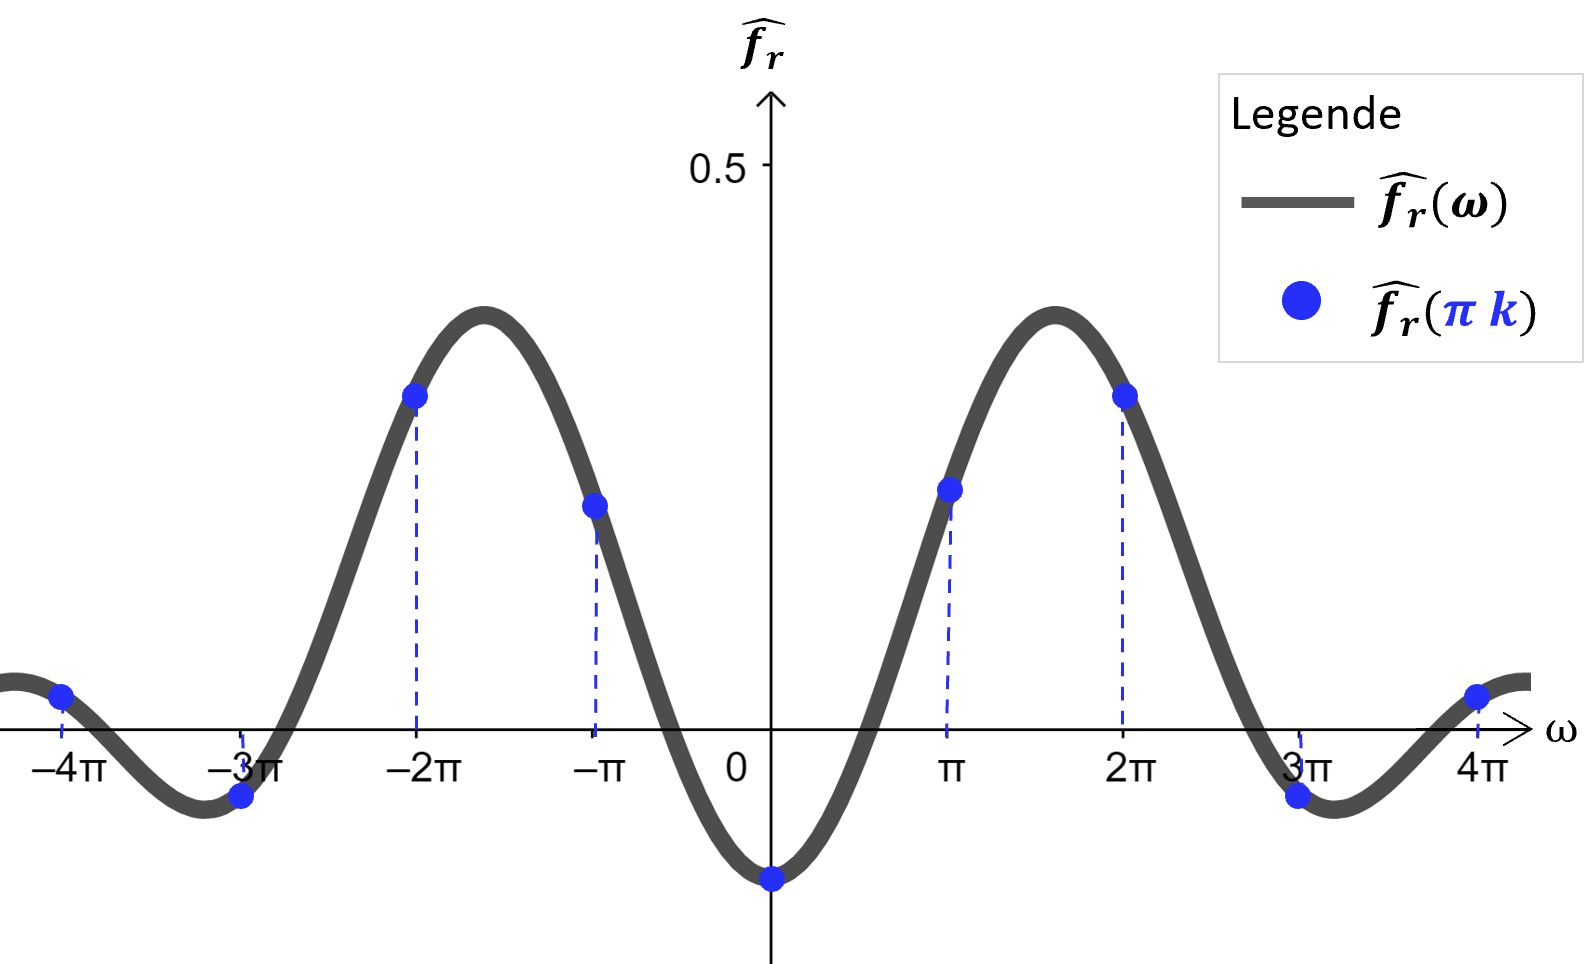
\includegraphics[width=0.7\textwidth]{../Mathematik_2/Bilder/dft_frequenzraster_zwischen_spektralmaxima.png}
\end{center}
	Die Grundfrequenz von \(f\) wird durch die DFT f�r kein \(k\) identifiziert. Alle diskreten Kreisfrequenzen, die die DFT detektieren kann, liegen \textbf{zwischen} den Nullstellen von \(\hat f_r\).
		Da \(| \hat r|\) asymptotisch gegen Null geht, wird die Grundfrequenz \(\omega_0\) von \(f\) auf benachbarte Frequenzen verteilt, man sagt auch, dass das Spektrum verschmiert. Dieses Ph�nomen nennt man Leck-Effekt.

		\[ g_{N/2}(t) = \sum\limits_{k=-N/2}^{N/2} c_{k}\, e^{-i\,\pi\,k\,t} \not= f(t)\,.\]

	Ist das Beobachtungsfenster kein ganzzahliges Vielfaches der Periode \(T_{\mathrm{min}}\) des Signals \(f\), so kommt es zum Leck-Effekt. Zur Reduzierung des Leck-Effektes werden bei zeitdiskreten Systemen Fensterfunktionen eingesetzt, und die abgetastete Signalfolge wird zun�chst mit der Fensterfunktion, beispielsweise einer diskreten von-Hann-Fensterfunktion, multipliziert. Anschlie�end wird die diskrete Fourier-Transformation ausgef�hrt.

\vspace{0.2cm}
\noindent\textbf{Bemerkungen:}

Man kann die Fouriertransformierte \(\hat f_r\) auch anders herleiten. Um ein stetiges Singal \(f: t\mapsto f(t)\) auf ein Zeitintervall, beispielsweise auf \([-1 ,1)\),  zu beschr�nken, multipliziert man \(f\) mit einer Rechteckfunktion:
			\[ f_r: t\mapsto f(t) \cdot r(t), \quad r: t\mapsto \begin{cases}  1, &\quad  -1 \leq t < 1 \,,\\0, &\quad \mathrm{sonst}\,.\end{cases}  \]
		Die Fouriertransformation eines Produkts im Zeitbereich ist eine Faltung der Fouriertransformierten im Frequenzbereich:
			\begin{equation}\label{faltung} \hat {f_r}(\omega)  =  \widehat{ \left( f\cdot r\right) }(\omega) = \dfrac{1}{\sqrt{2\pi}} \left( \hat f * \hat r\right) (\omega)   \,. \end{equation}
			Die Fouriertransformierte der Rechteckfunktion \(\hat r\) lautet:
			\begin{equation}\label{hat_r}
	\hat r(\omega) = \dfrac{1}{\sqrt{2\pi}}\int\limits_{-\infty}^\infty r(t) e^{- i\omega\,t } \,\mathrm{d}t  = \dfrac{1}{\sqrt{2\pi}}\dfrac{i}{\omega} \left[ e^{-i\omega\,t}\right]_{-1}^1 = \dfrac{i}{\omega} \left( e^{- i \, \omega} - e^{ i \, \omega}\right)  = \dfrac{2}{\sqrt{2\pi}}\dfrac{\sin(\omega)}{\omega} \,.
\end{equation}
\begin{minipage}{0.4\textwidth}
	\begin{eqnarray*}
		\Rightarrow \; \begin{cases} | \hat r(\omega) | &= \dfrac{2}{\sqrt{2\pi}}\dfrac{|\sin(\omega)|}{|\omega|} \\ \mathrm{arg}(\hat r(\omega)) &= \begin{cases}  0, \quad &\hat r(\omega) \geq 0\,,\\ \pi,\quad &\hat r(\omega) < 0 \,. \end{cases}\end{cases}
	\end{eqnarray*}
\end{minipage}
	\begin{minipage}{0.55\textwidth}
	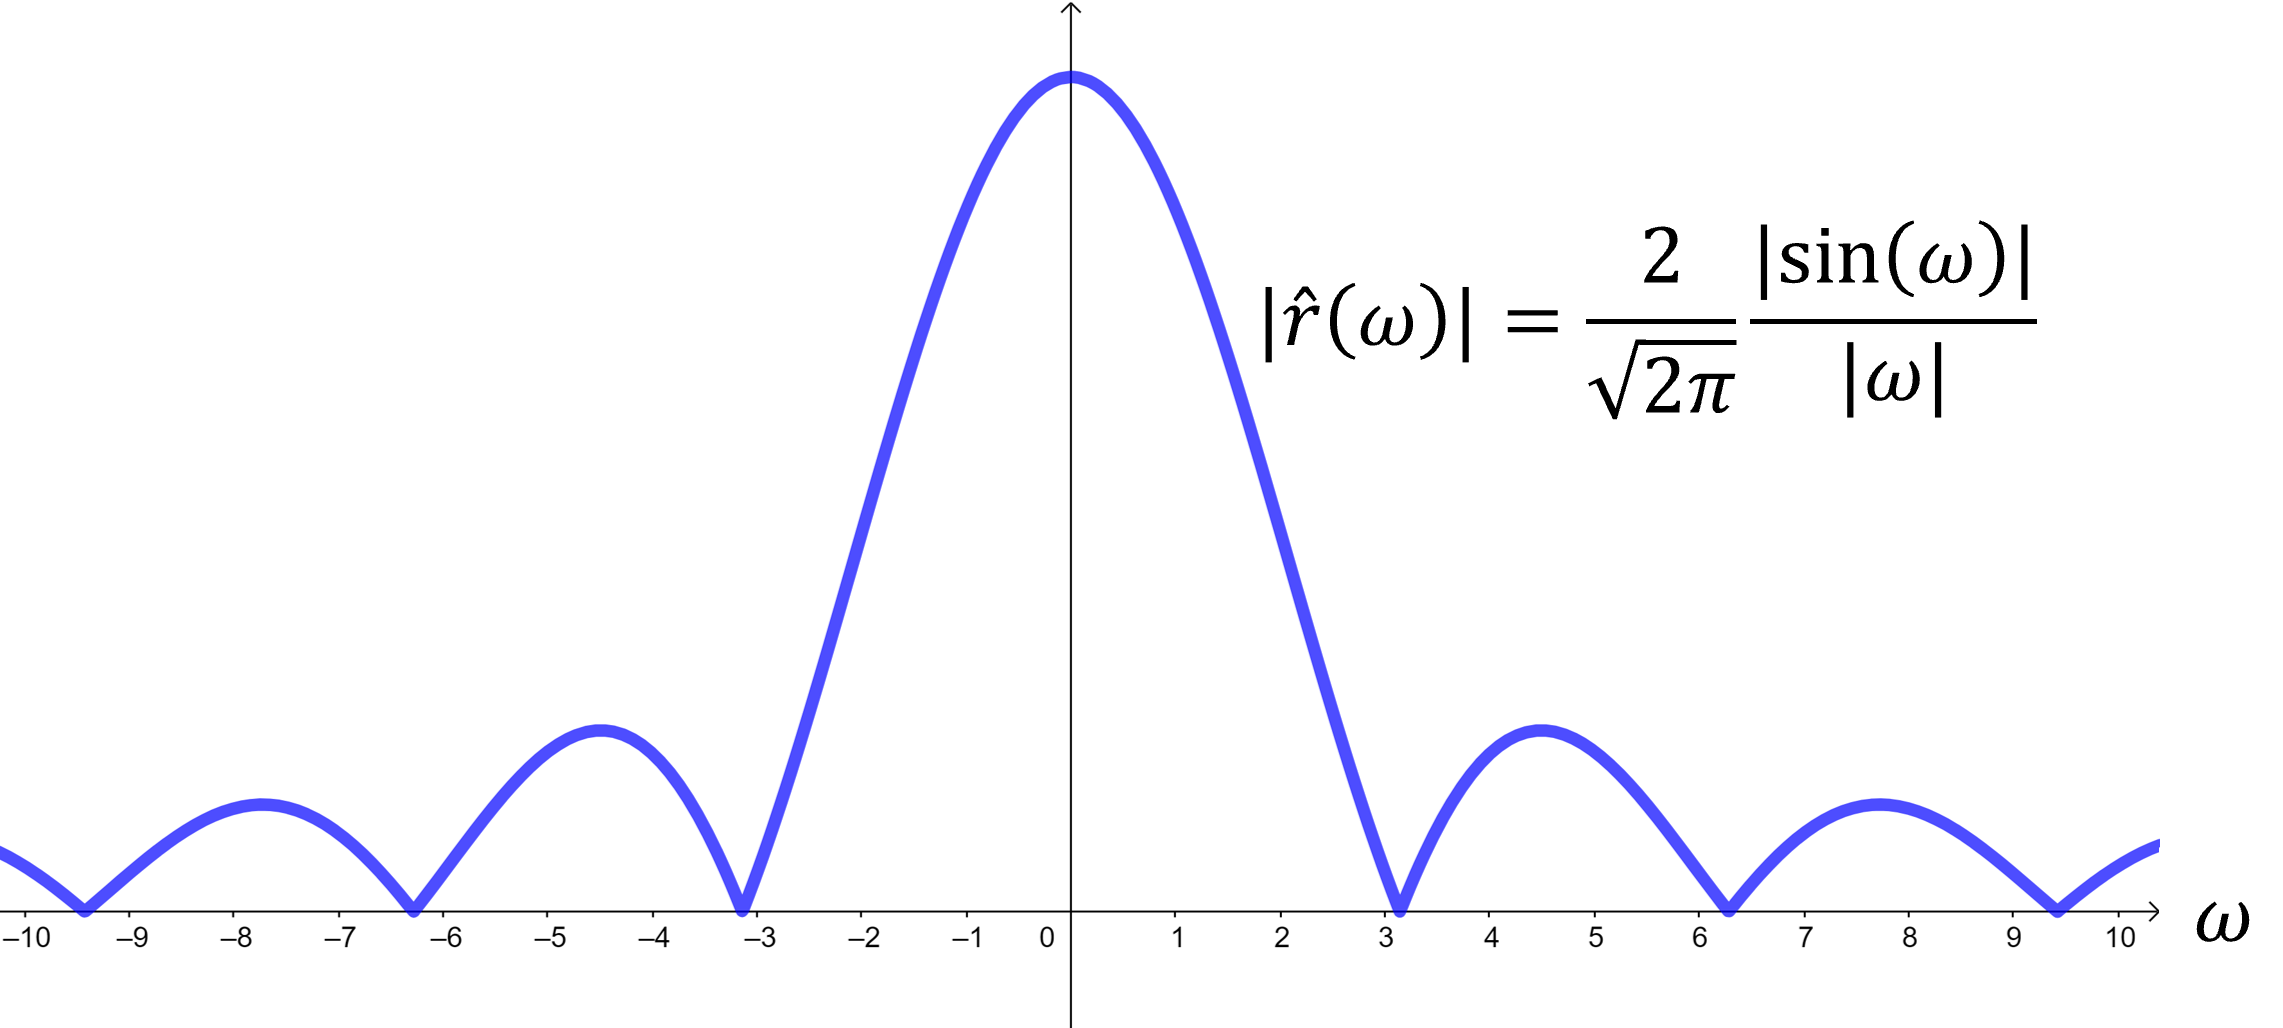
\includegraphics[width=\textwidth]{../Mathematik_2/Bilder/fouriertransformation_rechteckfenster_sinc_betrag.png}
\end{minipage}
			Nehmen wir an, dass \(f\) eine harmonische Schwingung ist, so ist deren Fouriertransformierte die �berlagerung zweier \(\delta\)-Impulse:
			\begin{equation}\label{hat_f} f(t) = A\cdot \cos\left( \omega_0\, t\right) \stackrel{\displaystyle{ \mathcal F}}{\longrightarrow}   \hat f(\omega) = A \sqrt{2\pi} \, \dfrac12 \left( \delta(\omega-\omega_0) + \delta(\omega +\omega_0)\right)\,.\end{equation}
			Wir setzen \eqref{hat_f}, \eqref{hat_r} in \eqref{faltung} ein und erhalten, unter Verwendung der Eigenschaften der Delta-Distrubution, die Fouriertransformierte von \(f_r\):
\begin{eqnarray*}
	\hat {f_r}(\omega)  =  \dfrac{1}{\sqrt{2\pi}} \left(  \frac{\sqrt{2\pi}}{2} \cdot A  \,\left(  \hat r(\omega - \omega_0) + \hat r(\omega + \omega_0) \right) \right) = \dfrac{A}{\sqrt{2\pi}}\cdot \left(  \dfrac{\sin(\omega-\omega_0)}{\omega-\omega_0} + \dfrac{\sin(\omega+\omega_0)}{\omega+\omega_0}\right)\,.
\end{eqnarray*}

\end{exercisebox}

\begin{exercisebox}{Matlab: Experiment: DFT gest�rte Daten}{ } % p.428 16.12 noise

\begin{center}
	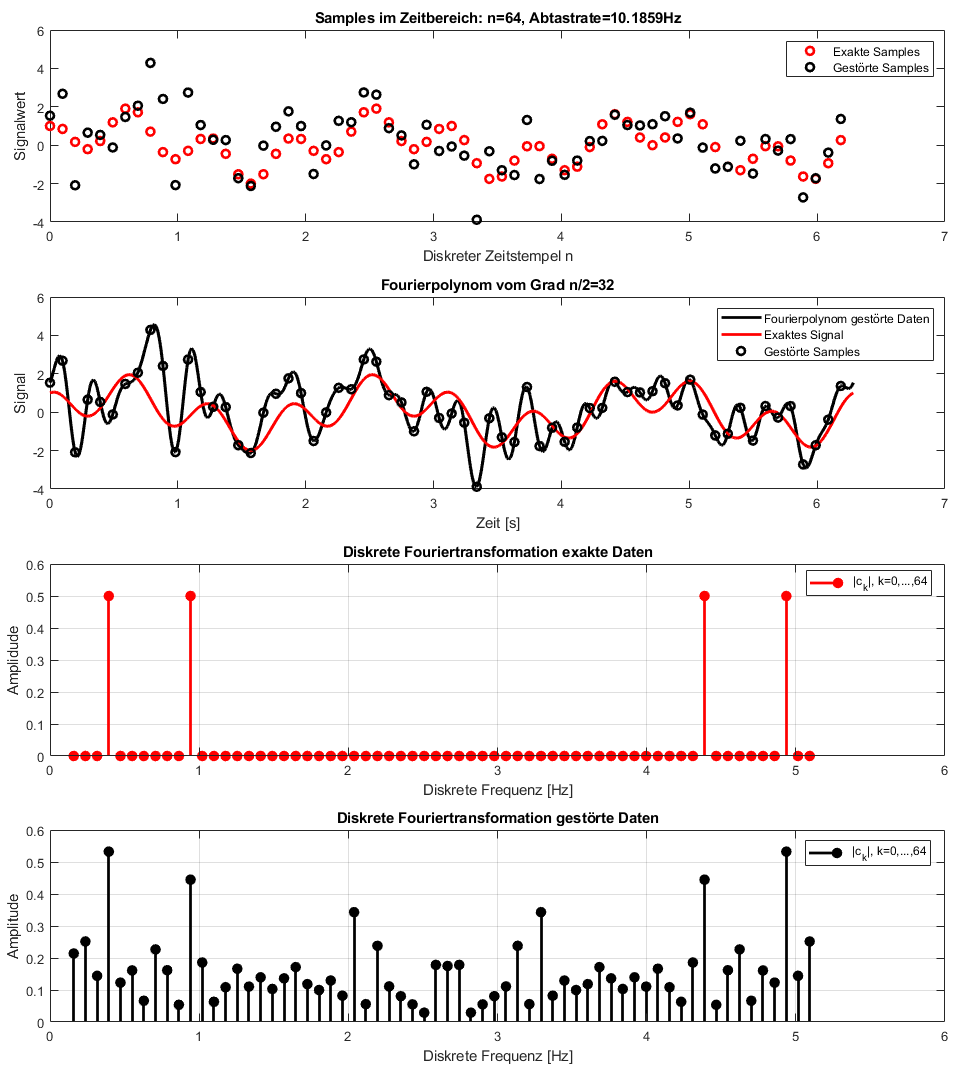
\includegraphics[width=\textwidth]{../Mathematik_2/Bilder/dft_verrauschtes_signal_und_spektrum.png}
\end{center}
\end{exercisebox}
 \newpage  % Matlab Experimente
% \setcounter{exercise}{0} \section*{Fouriertransformation Aufgaben mit L�sungen}\label{MA2-fouriertransformation-loesungen}

\ifintegriereaufgaben Erkl�rungen und Beispiele, die zum Verst�ndnis der L�sungswege hilfreich sind, finden Sie im Skript\wennreferenzvorhanden{MA2-fouriertransformation}{ (Abschnitt \abschnittsverweis{MA2-fouriertransformation})}. \fi



\begin{exercisebox}[Fourier-Transformation]
	Berechnen Sie die Fourier-Transformierte der folgenden Funktionen.
\begin{itemize}
	\item[(a)] $\delta > 0$
		\[ f:t\mapsto \begin{cases} e^{-\delta t}, \quad &t\geq 0\,,\\
				0\quad & t< 0\,.
			\end{cases}
		\]
	\item[(b)]
		\[ f:t\mapsto \begin{cases} \cos^2(t), \quad &|t| \leq \pi/2\,,\\
				0\quad & \textnormal{sonst}
			\end{cases}
		\]
	\item[(b)] $f: t\mapsto t\cdot e^{-|t|}$
\end{itemize}
\vspace{0.3cm}
\textbf{L�sung:} \newline

		Es kann hilfreich sein Symmetrieeigenschaften der Funktion zu untersuchen bevor man die Fourier-Transformierte berechnet, denn es gilt
	\begin{eqnarray*}
		\textnormal{gerade Funktionen}\; f(-t) &=& f(t) \Rightarrow \quad  \hat f(\omega) = \frac{2}{\sqrt{2\pi}} \int\limits_{0}^\infty f(t)\cdot \cos(\omega t)\,\mathrm{d}t\,,\\
		\textnormal{ungerade Funktionen}\; f(-t) &=& -f(t) \Rightarrow \quad \hat f(\omega) = \frac{-2i}{\sqrt{2\pi}} \int\limits_{0}^\infty f(t)\cdot \sin(\omega t)\,\mathrm{d}t\,.
	\end{eqnarray*}
	\begin{itemize}
			\item[(a)]
				\begin{eqnarray*}
					\hat f(\omega) &=& \frac{1}{\sqrt{2\pi}}\frac{\delta - i \omega}{\omega^2 + \delta^2} \\
						\Rightarrow |\hat f(\omega)| &=& \frac{1}{\sqrt{2\pi}}\frac{1}{\omega^2 + \delta^2} \quad \textnormal{Betrag}\,,\\
			\Rightarrow \varphi (\omega) &=& -\arctan\frac{\omega}{\delta} \quad \textnormal{Phase}\,.
		\end{eqnarray*}
	\item[(b)] Die Fouriertransformierte von \(f\) lautet:
		\[
		\hat f(\omega) = \frac{2}{\sqrt{2\pi}} \int\limits_{0}^{\pi/2} \cos^2(t) \cos(\omega t) \, \mathrm{d}t = \dfrac{4}{\sqrt{2\pi}} \dfrac{1}{\omega\,( 4 - \omega^2)} \sin\left(\omega \frac{\pi}{2}\right)\]
	Da $f$ eine gerade Funktion ist, l��t sich \(\hat f\) wie folgt berechnen \[ \hat f(\omega) = \dfrac{2}{\sqrt{2\pi}} \int\limits_0^\infty f(t) \cdot \cos(\omega\, t) \,\mathrm{d} t = \dfrac{2}{\sqrt{2\pi}} \int\limits_0^{\frac{\pi}{2}}  \cos^2(t) \cdot \cos(\omega\, t) \,\mathrm{d} t\,.\] Folgen wir dem Hinweis und schauen nach einem passenden Addtionstheorem zur Vereinfachung des Integranden. Es gilt
	\begin{equation}\label{additionstheorem} \cos^2( t ) = \dfrac12 \cdot \left( 1 + \cos(2\, t)\right) \,,\end{equation} und  damit
	\begin{equation}\label{ft} \hat f(\omega ) \stackrel{\eqref{additionstheorem}}{=} \dfrac{1}{\sqrt{2\pi}} \int\limits_0^{\frac{\pi}{2}}  \left(1 + \cos(2\,t)\right) \cdot \cos(\omega\, t) \,\mathrm{d} t  = \dfrac{1}{\sqrt{2\pi}}\left( \textcolor{red}{ \int\limits_0^{\frac{\pi}{2}}  \cos(\omega \, t) \,\mathrm{d} t} + \textcolor{blue}{\int\limits_0^{\frac{\pi}{2}} \cos(2\,t) \cdot \cos(\omega\, t) \,\mathrm{d} t} \right)  \,. \end{equation}
	Betrachten wir zu allererst den Fall \(\omega\not = 0\) und l�sen die beiden Integrale rechts getrennt. Das erste Integral rechts ist nicht schwer - es gilt:
	\[ \textcolor{red}{\int\limits_0^{\frac{\pi}{2}}  \cos(\omega \, t) \,\mathrm{d} t} = \left[ \dfrac{1}{\omega} \sin(\omega \, t ) \right]_0^{\frac\pi2} = \dfrac1\omega \sin\left( \omega \,\dfrac\pi2\right)\,.\]
	Zum L�sen des zweiten Integrals wenden wir zweimal eine partielle Integration an und das liefert:
	\begin{eqnarray*}
		&& \textcolor{blue}{\int\limits_0^{\frac{\pi}{2}} \cos(2\,t) \cdot \cos(\omega\, t) \,\mathrm{d} t}  \stackrel{ \mathrm{P.I.}}{=} \underbrace{ \left[ \cos(2\,t)\cdot \dfrac{1}{\omega} \sin(\omega\, t) \right]_0^{\frac{\pi}{2}}}_{-\dfrac{1}{\omega}\sin( \omega\, \frac\pi2)}  +\dfrac{2}{\omega} \int\limits_0^{\frac{\pi}{2}} \sin(2\,t)\cdot \sin(\omega\, t) \,\mathrm{d} t \\
		&\stackrel{ \mathrm{P.I.}}{=}&- \dfrac{1}{\omega}\sin( \omega\, \frac\pi2) + \dfrac2\omega \left(  \underbrace{ \left[ -\sin(2\,t)\cdot \dfrac1\omega\, \cos( \omega\,t)\right]_0^{\frac\pi2}}_{=0} + \dfrac{2}{\omega} \textcolor{blue}{ \int\limits_0^{\frac{\pi}{2}} \cos(2\,t) \cdot \cos(\omega\, t) \,\mathrm{d} t} \right)\\
		&=&- \dfrac{1}{\omega}\sin( \omega\, \frac\pi2) + \dfrac{4}{\omega^2} \textcolor{blue}{ \int\limits_0^{\frac{\pi}{2}} \cos(2\,t) \cdot \cos(\omega\, t) \,\mathrm{d} t}\,.
\end{eqnarray*}
Wir haben eine algebraische Gleichung erhalten, die sich nach unserem unbekannten Integral aufl�sen l��t!
\[ \Rightarrow \textcolor{blue}{\int\limits_0^{\frac{\pi}{2}} \cos(2\,t) \cdot \cos(\omega\, t) \,\mathrm{d} t} = - \dfrac{1}{ 1- \dfrac{4}{\omega^2} } \dfrac{1}{\omega} \, \sin\left( \omega \dfrac\pi2\right) = \dfrac{\omega}{4-\omega^2} \sin\left( \omega \dfrac\pi2\right) \,.  \]
Setzten wir die Integrale in \eqref{ft} ein, so erhalten wir f�r \(\omega \not = 0\)
\[ \hat f(\omega ) = \dfrac{1}{\sqrt{2\pi}} \dfrac1\omega \sin\left( \omega \,\dfrac\pi2\right) + \dfrac{\omega}{4-\omega^2} \sin\left( \omega \dfrac\pi2\right) =  \dfrac{1}{\sqrt{2\pi}} \dfrac{ 4}{\omega\,(4-\omega^2)} \sin\left( \omega \dfrac\pi2\right) \]
Betrachten wir jetzt  \(\omega=0\):
\[ \hat f(0) \stackrel{\eqref{additionstheorem}}{=} \dfrac{1}{\sqrt{2\pi}} \int\limits_0^{\frac\pi2} \left( 1 + \cos(2\,t)\right) \mathrm{d} t = \dfrac{1}{\sqrt{2\pi}}\cdot \dfrac{\pi}{2}  \]
Mit der Regel von L'Hospital ist
\[ \lim\limits_{\omega\to 0} \dfrac{\sin\left(\omega \dfrac{\pi}{2}\right)}{\omega} =  \dfrac{\pi}{2} \]
gilt f�r alle \(\omega \in \mathbb R\):
\[ \hat f(\omega ) = \dfrac{1}{\sqrt{2\pi}} \dfrac{ 4}{\omega\,(4-\omega^2)} \sin\left( \omega \dfrac\pi2\right) \]

	\item[(c)] $f$ ist eine ungerade Funktion
		\[
		\hat f(\omega) = \frac{-2i}{\sqrt{2\pi}} \int\limits_{0}^\infty te^{-t} \sin(\omega t) \, \mathrm{d}t = -\frac{1}{\sqrt{2\pi}}\frac{4i\omega}{\omega^4+ 2\omega^2 +1}\]

\end{itemize}
\end{exercisebox}

\begin{exercisebox}[Fourier-Transformation der Gau�schen Funktion]
	Bestimmen Sie die Fourier-Transformierte der Gau�schen Glockenkurve \( f: t \mapsto e^{-\frac{t^2}{2}} \). Benutzen Sie ohne Beweis die folgende Identit�t \( \int\limits_{-\infty}^\infty e^{-z^2}\mathrm{d} z = \sqrt{\pi}\) wobei  \(z\in \mathbb C\,.\)

\vspace{0.3cm}
\textbf{L�sung:} \newline
			\begin{eqnarray*}
				\hat f(\omega) &=& \frac{1}{\sqrt{2\pi}} \int\limits_{-\infty}^\infty e^{-\frac{t^2}{2}} e^{-i\omega t}\,\mathrm{d}t \stackrel{(*)}{=} \frac{1}{\sqrt{2\pi}} \int\limits_{-\infty}^\infty e^{-\frac12 (t+i\omega)^2} \cdot e^{-\frac12 \omega^2} \,\mathrm{d}t \\ &\stackrel{ (**)}{=}& \frac{2}{\sqrt{2\pi}} e^{-\frac12 \omega^2} \int\limits_{-\infty}^\infty e^{-z^2} \,\mathrm{d}z = \sqrt{2} e^{-\frac12 \omega^2}\,,
			\end{eqnarray*}
			wobei
			\begin{itemize}
				\item der Exponent in \( (*) \) durch die quadratische Erg�nzung umgeformt worden ist \[ -\frac12 t^2 - i\omega t = -\frac12\left( t^2 + 2i\omega t + (i\omega t)^2 \right) + \frac12 (i\omega)^2 = -\frac12\left( t+i\omega\right)^2 + \frac12(i\omega)^2 \,.\]
				\item das Integral durch die Substitution \( z = \frac12 (t+i\omega)\) in ein Integral �ber die komplexen Variable \(z\) �bergeht.
			\end{itemize}
Wichtig ist die Interpretation dieses Ergebnisses: Die Fourier-Transformierte einer Gau�schen Glockenkurve ist wieder die Gau�sche Glockenkurve!
\end{exercisebox}

\begin{exercisebox}[Fourier-Transformation]
	Im Skript wurde die Idee verfolgt die Fourier-Transformation mathematisch als Grenzprozess aus der Fourier-Reihe zu entwickeln. Den Grenzprozess schauen wir uns an einem konkreten Beispiel jetzt an.
\begin{itemize}
	\item[(a)] Zeigen Sie, dass gilt \[ c_{k} = \frac{\Delta \omega}{\sqrt{2\pi}} \cdot \tilde c_{k}, \quad \tilde c_{k} = \frac{1}{\sqrt{2\pi}} \cdot\int\limits_{-\frac{T}{2}}^{\frac{T}{2}} f(t)\cdot e^{-i\, \omega_k \,t} \,\mathrm{d} t, \quad \textnormal{mit Kreisfrequenz}\; \omega_k = \frac{2\pi k}{T}\,.\]
	\item[(b)] Betrachten Sie nun die $T$-periodische Funktion $f$ mit \( f|_{T}:[-T/2, T/2)\to \mathbb R,   t\mapsto e^{-|t|}\) und bestimmen Sie eine Formel f�r die Fourierkoeffizienten \(\tilde c_k\).
%\item[(c)] Zeigen Sie, dass gilt  \[ \tilde c_{k} = \sqrt{\frac{2}{\pi}}\left( 1- (-1)^k e^{-T/2}\right) \cdot \frac{1}{1+ \omega_k^2} \,.\]
	\item[(c)] Berechnen Sie die Fourier-Transformierte $\hat g$ von $g: \mathbb R \to \mathbb R, t\mapsto e^{-|t|}$.
	\item[(d)] Setzen Sie \(T=50\) und bestimmen Sie mit Hilfe einer Software die Punkte \( \left( \omega_k, \tilde c_k \right), \, 1\leq k \leq 50\). Erzeugen Sie ein Bild, das die Punkte und die den Graph von \(\hat g\) zeigt und interpretieren Sie das Ergebnis.
\end{itemize}

\vspace{0.3cm}
\textbf{L�sung:} \newline
\begin{itemize}
	\item[(a)]  \[ \Delta\omega= \frac{2\pi}{T}\; \Rightarrow \; c_k = \frac{1}{T} \, \int\limits_{-T/2}^{T/2} f(t) \cdot e^{-i\, \omega_k \,t}\,\mathrm{d}t = \frac{\Delta \omega}{2\pi} \textcolor{blue}{\int\limits_{-T/2}^{T/2}f(t) \cdot e^{-i \, \omega_k \, t}\,\mathrm{d}t}  =  \frac{\Delta \omega}{\sqrt{2\pi}} \cdot \textcolor{blue}{ \tilde c_k }\,.\]
	\item[(b)]
		\begin{eqnarray*}
			c_0 &=& \frac{1}{T} \int\limits_{-\frac{T}{2}}^{\frac{T}{2}} e^{-|t|} \, \mathrm{d} t = \frac{2}{T} \, \int\limits_{0}^{\frac{T}{2}} e^{-t} \,\mathrm{d}t = \frac2T \,\Big[ - e^{-t}\Big]_0^{\frac{T}{2}} = \frac2T\, \left( 1-e^{-\frac{T}{2}}\right)\\
			c_k &=& \frac{1}{T} \int\limits_{-\frac{T}{2}}^{\frac{T}{2}} e^{-|t|}\cdot e^{-i \, \omega_k \,t} \, \mathrm{d} t = \frac{1}{\sqrt{2\pi}} \frac{1}{1+\omega_k^2} \\[1ex]
			&=& \frac{\Delta \omega}{\sqrt{2\pi}} \, \frac{2}{\sqrt{2\pi}} \frac{1}{1+\omega_k^2} \left( 1-(-1)^k\, e^{-\frac{T}{2}}\right) \\[2ex]
			\Rightarrow  \; \tilde c_k &=& \frac{2}{\sqrt{2\pi}} \frac{1}{1+\omega_k^2} \left( 1-(-1)^k\, e^{-\frac{T}{2}}\right) \,.
		\end{eqnarray*}

	%	Die Funktion \(f\) ist gerade und damit gilt \begin{equation}\label{bn_gerades_Signal} b_n = 0, \quad n\geq 1\,. \end{equation} Die Koeffizienten \(a_n\) lauten:
	%	\begin{eqnarray*}
	%		a_0 &=& \frac{2}{T} \int\limits_{-\frac{T}{2}}^{\frac{T}{2}} e^{-|t|} \,\mathrm{d}t = \frac{4}{T} \int\limits_{0}^{\frac{T}{2}} e^{-t} \,\mathrm{d}t = \frac4T \Big[ - e^{-t}\Big]_0^{\frac{T}{2}} = \frac4T\left( 1-e^{-\frac{T}{2}}\right) \,,\\
	%		a_n &=& \frac{2}{T} \int\limits_{-\frac{T}{2}}^{\frac{T}{2}} e^{-|t|} \cdot \cos\left( \frac{2\pi n t}{T}\right) \,\mathrm{d}t =\frac{4}{T} \int\limits_{0}^{\frac{T}{2}} e^{-t} \cdot \cos\left(\frac{2\pi n t}{T}\right) \,\mathrm{d}t \\  &\stackrel{(*)}{ = }& \frac4T \left(  \Big[ -\cos\left(\frac{2\pi n t}{T}\right) e^{-t}\Big]_0^{\frac{T}{2}} + \frac{2\pi n}{T} \Big[ \sin\left(\frac{2\pi n t}{T}\right) e^{-t}\Big]_0^{\frac{T}{2}} - \left( \frac{2\pi n }{T}\right)^2  \int\limits_0^{\frac{T}{2}} \cos\left(\frac{2\pi n t}{T}\right) e^{-t}\,\mathrm{d}t \right) \\
	%		&\stackrel{(**)}{=}& \frac{4}{T} \frac{1}{1+\left( \frac{2\pi n}{T}\right)^2} \left( 1-(-1)^ne^{-\frac{T}{2}}\right)  = \frac{4 }{T} \frac{1}{1+\omega_n^2} \left( 1-(-1)^ne^{-\frac{T}{2}}\right)\,.
	%					\end{eqnarray*}
	%					wobei in \( (*) \) zweimal partiell integriert und in \( (**)\) die Identit�t \( \cos(\pi n ) = (-1)^n\) ausgenutzt worden ist.
	\item[(c)] \begin{eqnarray*} \hat g(\omega) &=& \frac{1}{\sqrt{2\pi}} \int\limits_{-\infty}^\infty  e^{-|t|}\cdot e^{-i\, \omega\, t}\,\mathrm{d}t = \frac{1}{\sqrt{2\pi}} \left( \int\limits_{-\infty}^0 e^t \cdot e^{-i\, \omega\, t}\,\mathrm{d}t + \int\limits_{0}^\infty e^{-t} \cdot e^{-i\,\omega\, t}\,\mathrm{d}t\right) \\
			&=& \frac{1}{\sqrt{2\pi}} \left( \Big[ \frac{1}{1-i\,\omega} e^{(1-i\,\omega)\,t}\Big]_{-\infty}^0 + \Big[ -\frac{1}{1+i\,\omega} e^{-(1+i\,\omega)t}\Big]_0^\infty\right) \\
			&=& \frac{1}{\sqrt{2\pi}} \left( \frac{1}{1-i\,\omega} + \frac{1}{1+i\,\omega} \right) = \frac{1}{\sqrt{2\pi}} \left(  \frac{1+i\,\omega}{1+\omega^2}  + \frac{1-i\,\omega }{1+\omega^2} \right) \\
								&=& \frac{2}{\sqrt{2\pi}} \frac{1}{1+\omega^2}\,.
						\end{eqnarray*}
	%		Es gilt \[ \begin{cases} c_{k} &= \frac12 \cdot \left( a_k - i \, b_k\right)\,, \\ c_{-k} &= \frac12\cdot \left(a_k + i\, b_k\right)\end{cases} \quad \stackrel{\displaystyle{ \eqref{bn_gerades_Signal}}}{\Rightarrow}  \quad  \begin{cases} c_{k} &= \frac12\cdot a_k\,, \\ c_{-k} &= \frac12\cdot a_k\,. \end{cases} \]
	%					Mit \(T= \dfrac{ 2\pi}{ \Delta \omega}\) erhalten wir
	%					\begin{eqnarray*}
	%					c_{k} = c_{-k} &=& \frac12 \frac{4}{T} \frac{1}{1+\omega_k^2} \left( 1-(-1)^k \, e^{-\frac{T}{2}}\right) = \frac{2\,\Delta \omega}{2\pi}  \frac{1}{1+\omega_k^2} \left( 1-(-1)^k\, e^{-\frac{T}{2}}\right) \\ &=&  \frac{\Delta \omega}{\sqrt{2\pi}} \underbrace{ \frac{2}{\sqrt{2\pi}} \frac{1}{1+\omega_k^2} \left( 1-(-1)^k\, e^{-\frac{T}{2}}\right)}_{\displaystyle{=: \tilde c_k}} \,.  \end{eqnarray*}
					\item[(d)] Bild erzeugt mit Geogebra:
						\vspace{0.2cm}
						\begin{center}
							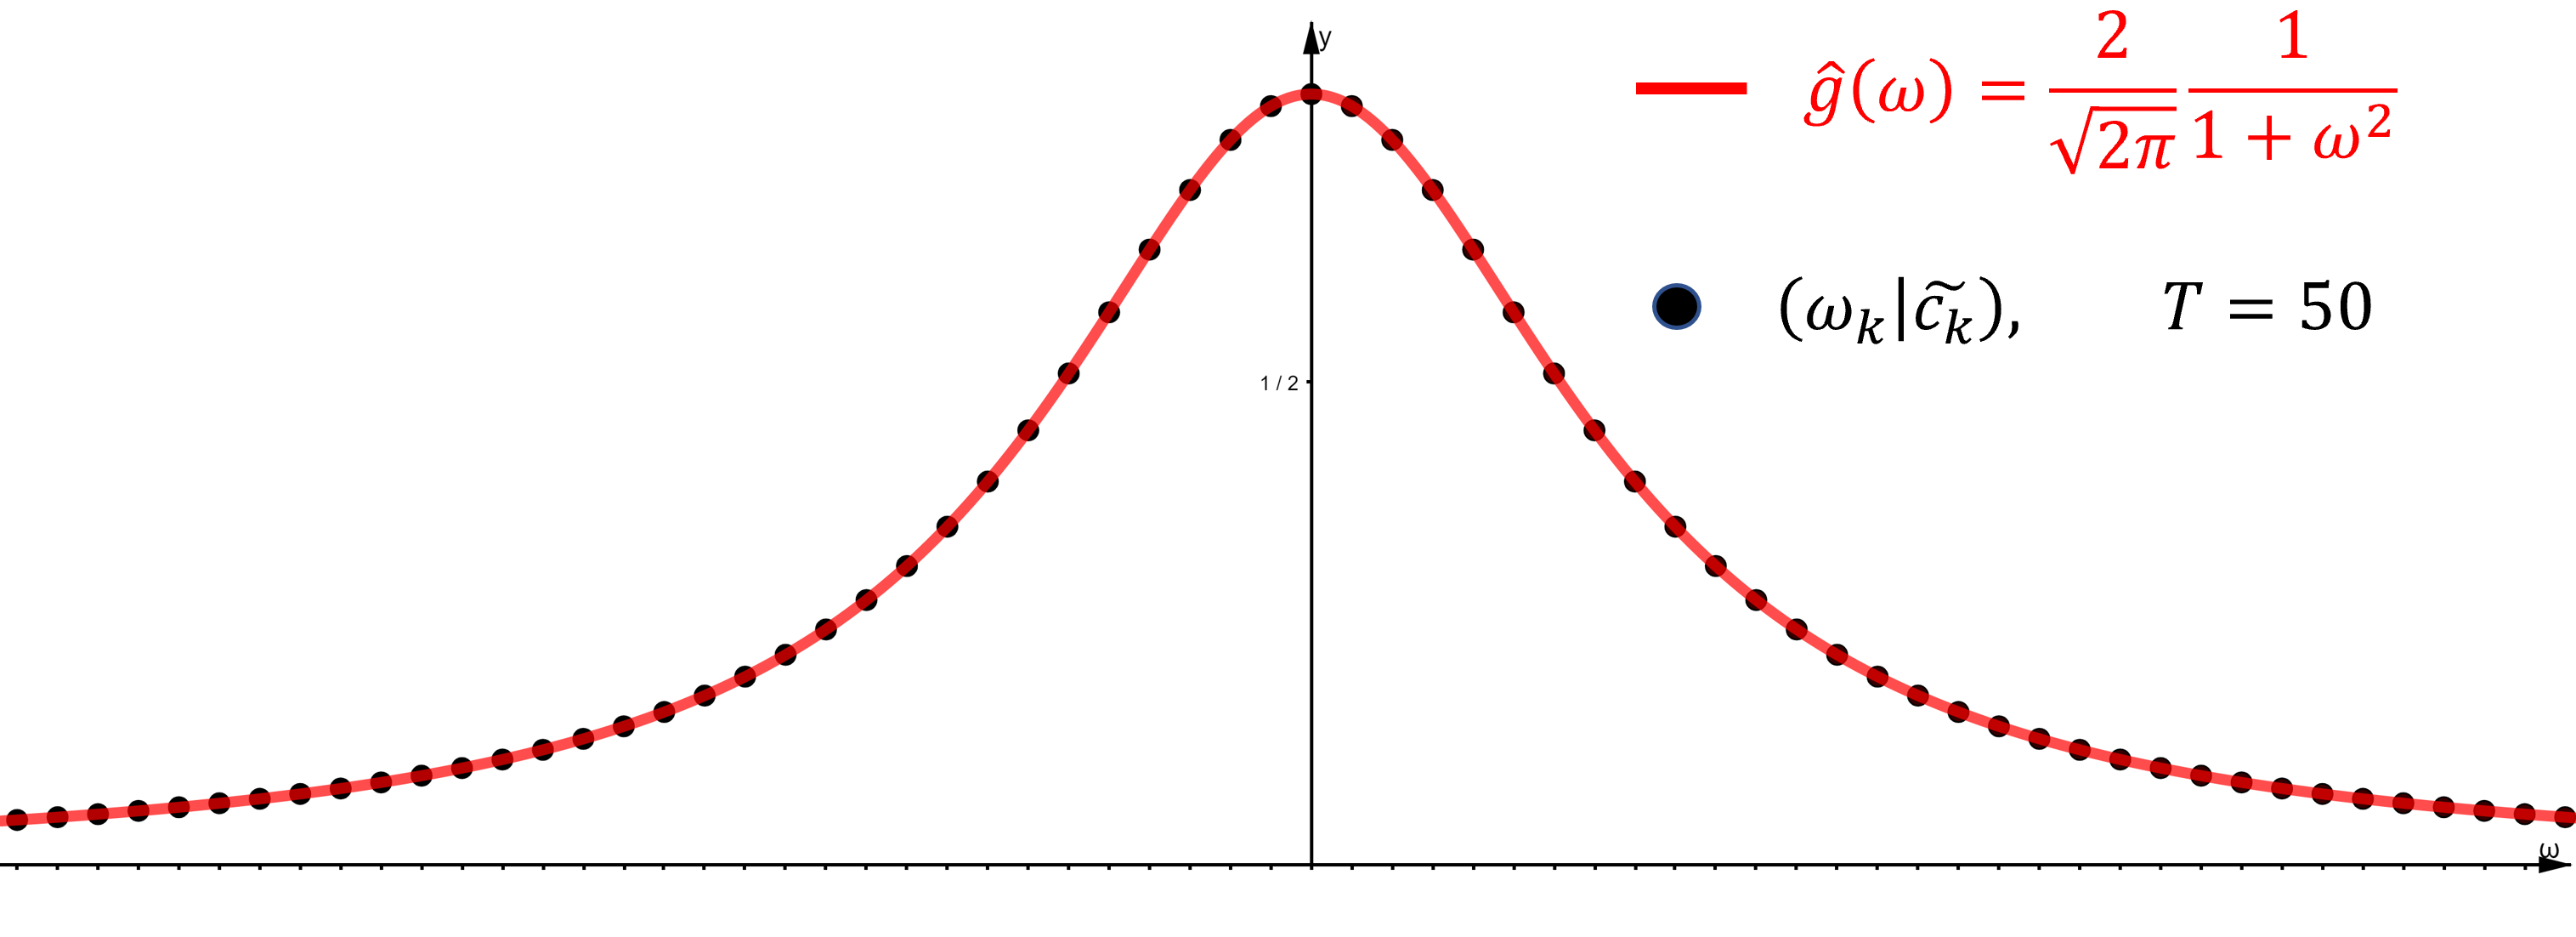
\includegraphics[width=0.8\textwidth]{../Mathematik_2/Bilder/fouriertransformation_grenzuebergang_von_fourierkoeffizienten.png}
			\end{center}
		\item[(e)] Das Spektrum von \(f\) sind diskrete Punkte im Frequenzraum \(\left( \omega_k \,|\, \tilde c_k\right) \, k \in \mathbb Z\). Die Punkte liege auf dem Graphen von \(\hat g\) und das sieht man auch analytisch: \[\lim\limits_{T\to \infty} \tilde c_k = \lim\limits_{T\to \infty}\frac{2}{\sqrt{2\pi}} \frac{1}{1+\omega_k^2} \left( 1-(-1)^k\, e^{-\frac{T}{2}}\right)  = \frac{1}{1+\omega_k^2} =  g(\omega_k) \,.\] Wichtig: der Grenz�bergang wird bez�glich der Variable \(T\) unternommen und zwar f�r eine fixierte Diskretisierung in \(\omega\)!
	\end{itemize}
\end{exercisebox}
%\begin{exercisebox}[Diskrete Fourier-Transformation]
%	Nehmen wir an das kontinuierlich gegebene Signal
%	\[ f: t\mapsto 5 + 2\cos(2\pi t - \pi/2) + 3\cos(4\pi t) \]
%	wird pro Sekunde vier Mal abgetastet.
%	\begin{itemize}
%		\item[(a)] Bestimmen Sie die Samples, die in einer Sekunde gemessen werden.
%		\item[(b)] Bestimmen Sie die diskrete Fourier-Transformation und zeigen Sie, dass sich die diskrete Fourier-Transformation als Matrix-Vektor-Multiplikation schreiben l��t.
%		\item[(c)] Wie l��t sich das Ergebnis interpretieren?
%	\end{itemize}
%\vspace{0.3cm}
%\textbf{L�sung:} \newline
%\begin{itemize}
%\item[(a)] F�r $S_l=(t_l, f(t_l))$ gilt $S_1 = \left(0,8\right), S_2= \left(\frac14,4\right), S_3=\left( \frac12, 8\right), S_4=\left( \frac34,0\right)$
%\item[(b)] Es gilt $\hat c_l = \displaystyle{ \sum\limits_{k=0}^3 e^{-i \,l\, \frac{2\pi}{N}  k} \cdot f(t_l) }$. Im vorliegenden Fall ist \(N=4\) und damit
%	\begin{eqnarray*}
%		\hat c_l = \displaystyle{ \sum\limits_{k=0}^3 e^{- i\,l \frac{2 \pi}{4} l} \cdot f(t_l) } \Rightarrow \left( \begin{array}{c} \hat c_0 \\\hat c_1 \\\hat c_2 \\ \hat c_3 \end{array}\right) = \left( \begin{array}{cccc} 1 & 1 & 1 & 1 \\ 1 & -i & -1 & i \\1 & -1 & 1 & -1 \\ 1 & i & -1 & -i \end{array}\right) \left( \begin{array}{c} 8 \\ 4 \\ 8 \\0\end{array}\right) \Rightarrow    \left( \begin{array}{c} \hat c_0 \\\hat c_1 \\\hat c_2 \\ \hat c_3 \end{array}\right) =\left( \begin{array}{c} 20 \\ -4i \\ 12  \\ 4i \end{array}\right)
%	\end{eqnarray*}
%\item[(c)] Die DFT liefert bis auf einen Skalierungsfaktor die Zerlegungskoeffizienten der harmonischen Schwingungen, die im Signal $f$ detektiert werden! Aus der DFT lassen sich die Samples zur�ckgewinnen durch die inverse, diskrete Fourier-Transformation (iDFT):
%	\[ f_k = \frac{1}{N}\sum\limits_{n=0}^{N-1} \hat c_n e^{i\, k\, \frac{2\pi}{N} n}\,. \]
%\end{itemize}
%\end{exercisebox}


 \newpage
%
% \setcounter{exercise}{0} \section*{Differentialgleichungen Aufgaben mit L�sungen}\label{MA2-differentialgleichungen-loesungen}

\ifintegriereaufgaben Erkl�rungen und Beispiele, die zum Verst�ndnis der L�sungswege hilfreich sind, finden Sie im Skript\wennreferenzvorhanden{MA2-differentialgleichungen}{ (Abschnitt \abschnittsverweis{MA2-differentialgleichungen})}. \fi

\begin{exercisebox}[Typeneinteilung]
	Klassifizieren Sie die folgenden Differentialgleichungen:
	\begin{itemize}
		\item[(a)] $\dot p(t) = a\cdot p(t) - b \cdot p^2(t)$
		\item[(b)] $M\ddot s(t) = As(t), \quad M, A \in \mathbb R^{2\times 2}, s:\mathbb R\mapsto \mathbb R^2\,.$
		\item[(c)] $y' = x y^2\,.$
		\item[(d)] $y\cdot y^{(4)} + x y'' + \ln(y) = 0\,.$
		\item[(e)] $\Delta u(x,y) = 0\,, \quad (x,y)\in \Omega\subset \mathbb R^2, \quad \Delta u = \displaystyle{\frac{\partial^2 u}{\partial x^2} +\frac{\partial^2 u}{\partial y^2}} $
	\end{itemize}

\vspace{0.3cm}
\textbf{L�sung:} \newline
	\begin{itemize}
		\item[(a)] Gew�hnliche Differentialgleichung erster Ordnung, explizit, nicht-linear. (biologische Population)
		\item[(b)] System gew�hnlicher Differentialgleichungen zweiter Ordnung: linear (zwei Linearschwinger)
		\item[(c)] Gew�hnliche Differentialgleichung erster Ordnung, explizit, nicht-linear (Trennbare Variablen)
		\item[(d)] Gew�hnliche Differentialgleichung vierter Ordnung, implizit, nicht-linear.
		\item[(e)] Partielle Differentialgleichung zweiter Ordnung, linear (Laplace-Operator)
\end{itemize}
\end{exercisebox}

\begin{exercisebox}[Differentialgleichungen] %Papula IV, Abschnitt 1, Aufgabe 1/2
	\begin{itemize}
		\item[(a)] Zeigen Sie, dass die Funktion $y: x\mapsto c_1 \cdot e^{5x} + c_2 \cdot e^{-x}$ f�r jede Wahl von $ c_1, c_2\in\mathbb R$ die folgende Differentialgleichung l�st:
			\[ y'' - 4y' - 5y = 0 \,.\]
		\item[(b)] Zeigen Sie, dass $y: x\mapsto \displaystyle{ \frac{c\cdot x}{1+x}} $ f�r jede Wahl von $c\in\mathbb R$ die folgende Differentialgleichung l�st
			\[ x (1+x)y' - y = 0, \; x\in(-1,1) \,\]

			und bestimmen Sie $c$ so, dass auch $y(1) = 8$ gilt.
	\end{itemize}
\vspace{0.3cm}
\textbf{L�sung:} \newline
	Diese Aufgaben finden Sie in Papula Band 2, Abschnitt IV.1 auf Seite \(519\) und detaillierte L�sungen auf Seite \(725\).
	\begin{itemize}
		\item[(a)] Papula Aufgabe IV.1.2) $\quad$ Differenzieren und Einsetzen.
		\item[(b)] Papula Aufgabe IV.1.1) $\quad c= 16 \Rightarrow y:x\mapsto 16 x / (1+x)$
	\end{itemize}
\end{exercisebox}

\begin{exercisebox}[Asymptotik]
	Betrachten Sie das Anfangswertproblem
	\[\begin{cases}
			s(0) = 0, \quad & t_0=0\,,\\
			\dot s(t) = 1+s^2(t)\,,\quad & t > t_0\,.
	\end{cases}\]
	\begin{itemize}
		\item[(a)] Zeigen Sie, dass $s:t\mapsto \tan(t)$ eine L�sung des Anfangswertproblems ist.
		\item[(b)] Bestimmen Sie das asymptotische Verhalten der angegebenen L�sung f�r $t\to \pi/2$
		%\item[(c)] Ist die L�sung eindeutig?
	\end{itemize}
\vspace{0.3cm}
\textbf{L�sung:} \newline
	\begin{itemize}
		\item[(a)] Differenzieren und Einsetzen.
		\item[(b)] W�chst die Geschwindigkeit mit dem Quadrat des Abstands vom Ursprung, so gelangt man nach endlicher Zeit ins Unendliche: \[ \lim\limits_{t\to \pi/2} s(t) = \infty \,.\]
		L�sung ist �brigens eindeutig. Warum?
	\end{itemize}
\end{exercisebox}

\begin{exercisebox}[Eindeutige L�sbarkeit]
	Betrachten Sie das Anfangswertproblem
	\[\begin{cases} y(1) = 1, \quad & x_0=1\,,\\
			(y')^2 - 4xy' + 4y = 0\,,\quad & x > x_0\,.
	\end{cases}\]
	\begin{itemize}
		\item[(a)] Klassifizieren Sie die Differentialgleichung.
		\item[(b)] Zeigen Sie, dass $y: x\mapsto 2cx-c^2$ die Differentialgleichung l�st und skizzieren Sie die Geradenschar.
		\item[(c)] Bestimmen Sie die Konstante $c$ so, dass $y$ das Anfangswertproblem l�st.
		\item[(d)] Ist die L�sung des Anfangswertproblems eindeutig?
	\end{itemize}
\vspace{0.3cm}
\textbf{L�sung:} \newline
	\begin{itemize}
		\item[(a)] Implizite, nicht-lineare, gew�hnliche Differentialgleichung erster Ordnung.
		\item[(b)] Differenzieren und Einsetzen. Schauen Sie sich die Geradenschar an, zum Beispiel mit folgender interaktiven GeoGebra-App, in die Sie die Geradenschar als Input eintippen k�nnen - anstatt \(c\) schreiben Sie \(k\): \url{https://www.geogebra.org/m/DTNqPW52}
		\item[(c)] $c= 1 \Rightarrow y:x\mapsto 2x-1$.
		\item[(d)] $y:x\mapsto x^2$ l�st auch das Anfangswertproblem! Es ist eine sogenannte singul�re L�sung und man kann Sie als Einh�llende der Geradenschar $y_c:x\mapsto 2cx-c^2$ der Skizze entnehmen.
	\end{itemize}
\end{exercisebox}

%\subsection{Praxis}
%\begin{exercisebox}[Moodle Eindeutigkeit] % HMI III; Blatt 12, Aufg. 3
%Die allgeimeine L�sung der Differentialgleichung
%\[ y'' + y = 1 \]
%lautet
%\[y(x) = c_1 \cos(x) + c_2\sin(x) + 1\,. \]
%Untersuchen Sie die Eindeutigkeit der L�sung bei Vorgabe von Anfangsbedingungen.
%\begin{itemize}
%	\item[(a)] $ y(0) = 0 \land y(\pi/2) = 1 $
%	\item[(b)] $ y(0) = 0 \land y(\pi) = 1 $
%	\item[(c)] $ y(0) = 0 \land y(\pi) = 2 $
%	\item[(d)] $ y(0) = 0 \land \left( y'(b)\right)^2 = 1, \quad 0 < b < \pi/2 $
%\end{itemize}
%\end{exercisebox}

%\subsection{Theorie}
%
%\begin{mybox}[�bersicht �ber Aufgabentypen]
%	Das Anfangswertproblem ist l�sbar, falls \(f:D_f\to \mathbb R\) bez�glich \(x\) und \(y\) stetig ist, dann besietzt das Anfangswertproblem wenigstens eine L�sungskurve in \(D_f\).
%\end{mybox}

 \newpage
% \setcounter{exercise}{0} \section*{Lineare Differentialgleichungen Aufgaben mit L�sungen}\label{MA2-lineare-differentialgleichungen-loesungen}

\ifintegriereaufgaben Erkl�rungen und Beispiele, die zum Verst�ndnis der L�sungswege hilfreich sind, finden Sie im Skript\wennreferenzvorhanden{MA2-differentialgleichungen}{ (Abschnitt \abschnittsverweis{MA2-differentialgleichungen})}\wennreferenzvorhanden{MA2-lineare-differentialgleichungen}{ (Abschnitt \abschnittsverweis{MA2-lineare-differentialgleichungen})}.\fi

\begin{exercisebox}[L�sungskurve] %Papula, IV Abschnitt 2, Aufgabe 1
	Skizzieren Sie das Richtungsfeld der folgenden Differentialgleichungen und zeichnen Sie eine L�sungskurve f�r den gegebenen Anfangswert ein.
	\begin{eqnarray*}
		\begin{array}{lr}
			(a)\; y' = y, \; y(0) = 2  &  (b)\; y'=\displaystyle{\frac{y}{2x}}, \quad x\in(0,\infty), \; y(1) = 1\,.
	\end{array}
	\end{eqnarray*}
\vspace{0.3cm}
\noindent \textbf{L�sung:} \newline
	Diese Aufgaben finden Sie in Papula Band 2, Abschnitt IV.2 auf Seite \(520\) und detaillierte L�sungen ab Seite \(725\)f.
	\begin{itemize}
		\item[(a)] Aufgabe 1b) $\quad y(x) = 2e^x$
		\item[(b)] Aufgabe 1a) $\quad y(x) = \sqrt{x}$
	\end{itemize}
\end{exercisebox}

\begin{exercisebox}[Lipschitz-Stetigkeit]
�berpr�fen Sie, ob die folgenden Funktionen auf $D_f:= [0,0]\times [1,1]$  Lipschitz-stetig sind, ob also gilt
	\[
		\exists \, L\leq 0: \; \forall y_1, y_2 \in D_f:\quad |f(x,y_1) - f(x,y_2)|\leq L |y_1 - y_2| \,,
	\]
	und geben Sie gegebenenfalls die Lipschitz-Konstante an.
	\begin{eqnarray*}
		\begin{array}{lr}
			(a)\; f: (x,y) \mapsto y^2  &  (b)\; f: (x,y) \mapsto 2\sqrt{y} \,.
	\end{array}
	\end{eqnarray*}
\vspace{0.3cm}
\noindent \textbf{L�sung:} \newline
	\begin{itemize}
		\item[(a)] $|f(x,y_1) - f(x,y_2)| = |y_1^2 - y_2^2| = |y_1 - y_2| \cdot |y_1 + y_2| \; \Rightarrow $ da $D_f$ beschr�nkt mit $|y_1 + y_2| \leq 2$ gilt  $L:=2$ .
		\item[(b)] Das Problem ist der Nullpunkt $(0,0) \in D_f$:  \[|f(0,0) - f(0,y_2)| = 2\sqrt{|0-y_2|} = \frac{2}{\sqrt{| 0 - y_2|}} \cdot |0 - y_2|\]
			Allerdings ist $f$ im Nullpunkt unbeschr�nkt,
			\[ \lim\limits_{y_2 \downarrow 0} \frac{2}{\sqrt{|0-y_2|}} = \infty\,, \]
				und damit erf�llt $f$ keine Lipschitz-Bedinung.
	\end{itemize}
\end{exercisebox}

\begin{exercisebox}[Inhomogenit�t] %Papula IV, Abschnitt 2, Aufgabe 18
	L�sen Sie die folgende inhomogene Differentialgleichung
\begin{eqnarray*}
	y' - 3y = x\cdot e^x
\end{eqnarray*}
durch (a)  Variation der Konstanten und (b) Ansatz vom Typ der rechten Seite.

\vspace{0.3cm}
\noindent \textbf{L�sung:} \newline
Diese Aufgaben entspricht Aufgabe \(18a)-b)\) in Papula Band 2, Abschnitt IV.1 auf Seite \(523\). L�sungen finden Sie ab Seite \(729\).
\begin{itemize}
	\item[(a)] Sie bestimmen zun�chst die allgemeine L�sung der homogenen Gleichung und dann eine partikul�re L�sung durch Variation der Integrationskonstante:
		\begin{eqnarray*}
		y_h(x) &=& C\cdot e^{3x}\\
		\Rightarrow y_p(x) &=& C(x) \cdot e^{3x} \Rightarrow  C'(x) \stackrel{!}{=} x\cdot e^{-2x} \Rightarrow C(x) = \int x\cdot e^{-2x}\,\mathrm{d}x \stackrel{P.I.}{=} -\frac14\left( 2x+1\right) e^{x} \\
		\Rightarrow y(x) &=& y_h(x) + y_p(x) = C\cdot e^{3x} - \frac14(2x+1)\cdot e^{x}
	\end{eqnarray*}
\item[(b)] Sie bestimmen zun�chst die allgemeine L�sung der homogenen Gleichung und dann eine partikul�re L�sung durch einen Ansatz vom Typ der rechten Seite: \begin{eqnarray*}
		y_h(x) &=& C\cdot e^{3x}\\
		\mathrm{r.S} \; x\cdot e^x \Rightarrow y_p(x) &=& (ax+b)\cdot e^x \Rightarrow \left( a-2b -2ax \right) \cdot e^x \stackrel{!}{=} x\cdot e^x \Rightarrow \begin{cases} a& =-\frac12 \\ b=-\frac14 \end{cases}  \\
		\Rightarrow y(x) &=& y_h(x) + y_p(x) = C\cdot e^{3x} - \frac14(2x+1)\cdot e^{x}
	\end{eqnarray*}
	\end{itemize}
\end{exercisebox}

\begin{exercisebox}[Inhomogenit�t] % Papula IV, Abschnitt 2, Aufgabe 19
	L�sen Sie folgenden Differentialgleichungen mit Hilfe des Ansatz vom Typ der rechten Seite
\begin{eqnarray*}
	\begin{array}{ll l }
		(a)\; y' =  2x-y \;  & (b)\; y' + 2y= 4 \cdot e^{5x} \; & (c)\; y' + y = e^{-x} \\
		(d)\; y' - 4y = 5\sin(x) \; (e)\; y' - 5y = \cos(x) + 4 \sin(x)\; & (f)\; y' - 6y = 3 e^{6x}
		\end{array}
\end{eqnarray*}
\vspace{0.3cm}
\noindent \textbf{L�sung:} \newline
Diese Aufgaben entsprechen Aufgabe \(19a)-f)\) in Papula Band 2, Abschnitt IV.1 auf Seite \(523\). Detaillierte L�sungen finden Sie ab Seite \(729\).
\begin{itemize}
	\item[(a)] \( y(x) = C\cdot e^{-x} + 2x - 2 \)
	\item[(b)] \( y(x) = C\cdot e^{-2x} + \frac47\cdot e^{5x} \)
	\item[(c)] \( y(x) = (x+C)\cdot e^{-x} \)
	\item[(d)] \( y(x) = C\cdot e^{4x} - \frac{20}{17} \sin(x) - \frac{5}{17} \cos(x) \)
	\item[(e)] \( y(x) = C\cdot e^{5x} - \frac{19}{26} \sin(x) - \frac{9}{26} \cos(x) \)
	\item[(f)] \( y(x) = (3x+C)\cdot e^{6x} \)
\end{itemize}
\end{exercisebox}

\begin{exercisebox}[Inhomogenit�t] % Papula IV, Abschnitt 2, Aufgabe 21
	L�sen Sie folgende Anfangswertprobleme mit Hilfe des Ansatz vom Typ der rechten Seite
\begin{eqnarray*}
	(a)\; y' + 4y = x^3 - x \land y(1) = 2 \;  (b)\; y'-y= e^x \land y(0) = 1 \; (c)\; y'+3y = -\cos(x)\land y(0) = 5
\end{eqnarray*}
\vspace{0.3cm}
\noindent \textbf{L�sung:} \newline
Diese Aufgaben entspricht Aufgabe \(21\) in Papula Band 2, Abschnitt IV.1 auf Seite \(524\). Detaillierte L�sungen finden Sie ab Seite \(730\).
\end{exercisebox}

\begin{exercisebox}[Gleichungen h�herer Ordnung] % Papula IV, Abschnitt 3, Aufgabe 12, Abschnitt 5, Aufgabe 11 oder Abschnitt 4 eine der Aufgabe 4,6,8
	Geben Sie f�r folgende Differentialgleichungen jeweils die allgemeine L�sung an und l�sen Sie anschlie�end das zugeh�rige Anfangswertproblem
\begin{eqnarray*}
	(a) && \ddot x + 4\dot x + 29x=0 \quad   x(0)=1 \quad \dot x(0) =-2\\[1ex]
	(b) && \ddot x + 6 \dot x + 10 x = \cos(t)\quad x(0) = 0\quad \dot x(0) = 4  \\[1ex]
	(c) && y'' + 2y' + 3y = e^{-2x} \quad  y(0) = 0 \quad  y'(0) = 1 \\[1ex]
	(d) && \ddot x + \dot x + \frac14 x=0  \quad  x(0)=1 \quad  \dot x(0) =-1\\[1ex]
	(e) && \ddot x + 2 \dot x + 17 x = 2\sin(5t)  \quad  x(\pi) = 0  \quad  \dot x(\pi) = 1  \\[1ex]
	(f) && y''' + 9y' = 18 x,\; y(\pi) = \pi^2 \quad  y'(\pi) = 2\pi  \quad  y''(\pi) = 10 \\[1ex]
	(g) && y''' + 8 y'' + 17 y' + 10 y = 34 \sin(x) + 12 \cos(x)  \quad  y(0) = 1  \quad  y'(0) = -3 ,\; y''(0) = 8  \\[1ex]
		(h) && \ddot x + 7\dot x + 12x=0  \quad  x(0)=5 \quad  \dot x(0) =0
\end{eqnarray*}
\vspace{0.3cm}
\noindent \textbf{L�sung:} \newline
Diese Aufgaben finden Sie in Papula Band 2, Abschnitt IV. Detaillierte L�sungen finden Sie ab Seite \(730\).
\begin{itemize}
	\item[(a)] Papula 2 Abschnitt IV.4. Aufg. 4 a) Seite \(529\) L�sung Seite \(737\)
	\item[(b)] Papula 2 Abschnitt IV.3. Aufg. 12 a) Seite \(528\) L�sung Seite \(735\)
	\item[(c)] Papula 2 Abschnitt IV.3. Aufg. 12 b) Seite \(528\) L�sung Seite \(735\)
	\item[(d)] Papula 2 Abschnitt IV.4. Aufg. 6 b) Seite \(529\) L�sung Seite \(737\)
	\item[(e)] Papula 2 Abschnitt IV.3. Aufg. 12 c) Seite \(528\) L�sung Seite \(735\)
	\item[(f)] Papula 2 Abschnitt IV.5. Aufg. 11 a) Seite \(534\) L�sung Seite \(744\)
	\item[(g)] Papula 2 Abschnitt IV.5. Aufg. 11 b) Seite \(534\) L�sung Seite \(744\)
	\item[(h)] Papula 2 Abschnitt IV.4. Aufg. 8 c) Seite \(530\) L�sung Seite \(738\)
\end{itemize}
\end{exercisebox}

 \newpage
% \setcounter{exercise}{0} \input{../Material_2/36_loesungen} \newpage  %TODO
% \setcounter{exercise}{0} \section*{Numerische Verfahren Aufgaben mit L�sungen}\label{MA2-numerische-loesung-von-differentialgleichungen-loesungen}

\ifintegriereaufgaben Erkl�rungen und Beispiele, die zum Verst�ndnis der L�sungswege hilfreich sind, finden Sie im Skript\wennreferenzvorhanden{MA2-numerische-loesung-von-differentialgleichungen}{ (Abschnitt \abschnittsverweis{MA2-numerische-loesung-von-differentialgleichungen})}. \fi

\begin{exercisebox}[Explizites Euler Verfahren] %HMI 3 Blatt 4 Aufg. 4
	Berechnen Sie f�r das Anfangswertproblem
	\[
		\begin{cases}
			y(0) = 1\,,\quad & x=0\,,\\
			y' = x^2+y\,,\quad & x\not=0\,
		\end{cases}
	\]
	eine N�herungsl�sung f�r $y(2)$. Die N�herungsl�sung soll mit Hifle des Eulerschen Polygonzugverfahrens zur Schrittweite $h=1/4$ hergeleitet werden. L�sen Sie das Anfangswertproblem exakt und bestimmen Sie den relativen Fehler der Approximation f�r \(x=2\).

\vspace{0.3cm}
\textbf{L�sung:} \newline
Bestimmung der exakten L�sung:
\begin{enumerate}
	\item Allgemeine L�sung der homogenen Gleichung: \[ y' - y = 0 \Rightarrow y_h(x) = ce^x\,.\]
	\item Partikul�re L�sung mit Variation der Konstanten \[ y_p(x) = c(x) e^x \Rightarrow y_p'(x) = c'(x) e^x + c(x) e^x \Rightarrow c'(x) = x^2 e^{-x} \Rightarrow c(x) = -x^2 e^{-x} - 2xe^{-x} + ee^{-x} \,.\]
	\item Damit lautet die allgemeine L�sung: \[ y(x) = y_h(x) + y_p(x) = -x^2 - 3x -2 + ce^x \,.\]
	\item Bestimmung der Integrationskonstante: \[ y(0) \stackrel{!}{=} 1 \Rightarrow c = 3 \Rightarrow yy:x\mapsto 3e^x-x^2-2x-2\,.\]

\end{enumerate}

Bestimmung der N�herungsl�sung f�r \(x=2\) mit Polygonzugverfahren mit Schrittweite \(h=1/4\):
\begin{enumerate}
	\item St�tzstellen \( x_k=k\cdot h, \quad k=0,\cdots, 8\):
		\[ x_0 = 0, x_1=\frac14, x_2=\frac12, x_3 = \frac{3}{4}, x_4=1, x_5 = \frac54, x_6=\frac32, x_7=\frac74, x_8 = 2\]
	\item St�tzwerte \( y_k= y_{k-1} + 1/2 f( x_{k-1}, y_{k-1} ) k\cdot h, \quad k=0,\cdots, 8\)
		\begin{eqnarray*}
			y_0 &=& 1 \\
			y_1 &=& \frac{5}{4} \\
			y_2 &=& \frac{101}{64} \\
			y_3 &=& \frac{521}{256} \\
			y_4 &=& \frac{2749}{1024} \\
			y_5 &=& \frac{14769}{4096} \\
			y_6 &\approx& 4.90 \\
			y_7 &\approx& 6.68 \\
			y_8 &\approx& 9.12
		\end{eqnarray*}
	\item Der relative Fehler ist \[ r_{\mathrm{rel}} = \frac{|y(2) - y_2|}{|y(2)|} = 0.25\,.\]
\end{enumerate}
Und so sehen Sie auf einen Blick, wie sich die Approximation von der exakten L�sung wegbewegt:
	\begin{center}
	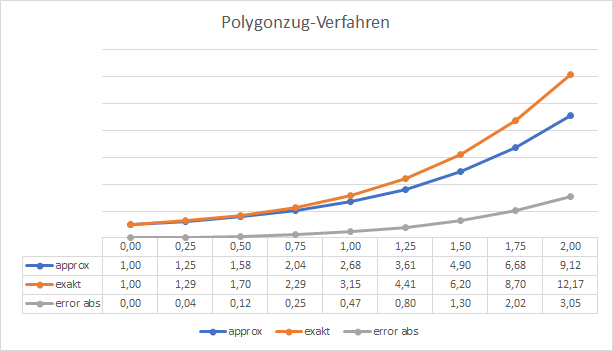
\includegraphics[width=0.7\textwidth]{../Mathematik_2/Bilder/eulerverfahren_polygonzug.png}
\end{center}
\end{exercisebox}

\begin{exercisebox}[Verbessertes Euler Verfahren] %HMI 3 Blatt 6 Aufg. 1
	Eine Verbesserung des expliziten Euler Verfahrens lautet
	\[
		\begin{cases}
			k_1 = f(x_k, y_k)\,,\\
			k_2 = f(x_k+\frac{h}{2}, y_k + \frac{h}{2}k_1)\,,\\
			y_{k+1} =  y_k + hk_2\,.
		\end{cases}
	\]
	\begin{itemize}
		\item[(a)] Verdeutlichen Sie graphisch die Funktionsweise des Verfahrens.
		\item[(b)] Bestimmen Sie f�r das Anfangswertproblem aus der ersten Aufgabe die Approximation f�r $x=2$ zur Schrittweite \(h=1/4\) und bestimmen Sie den relativen Fehler zur exakten L�sung.
		\item[(c)] Betrachten Sie das Anfangswertproblem
	\[
		\begin{cases}
			y(0) = y_0\,,\quad & x=0\,,\\
			y' = -2at\,,\quad & x\not=0\,.
		\end{cases}
	\]
	�berzeugen Sie sich davon, dass die verbesserte Polygonzugmethode das Anfangswertproblem zu unterschiedlichen Werten von \(a\) und Anfangswerten \(y_0\) exakt l�st. Was k�nnen Sie daraus schlie�en?
	\end{itemize}

\vspace{0.3cm}
\textbf{L�sung:} \newline
\begin{itemize}
	\item[(a)]
	\item[(b)] Die exakte L�sung ist $y:x\mapsto 3e^x-x^2-2x-2$. Sie merken schon, dass es keinen Spa� macht ein numerisches Verfahren per Hand hinzuschreiben - selbst wenn man das Intervall nur in \(8\) Teilintervalle zerteilt. Man sollte ein numerisches Verfahren programmieren. Da wir nicht an Effizienz oder Post-Prozessing interessiert sind, kann man das auch ganz einfach gestalten und zum Beispiel ein Programm zur Tabellenkalkulation benutzen.

		Der numerische Fehler des verbesserten Polygonzugverfahrens f�r die gestellte Aufgabe betr�gt nunmehr \( e_{\mathrm{rel}} = 0.02\), der Wert f�r \(x=2\) lautet \(y_8 = 11.87\), die exakte L�sung lautet \(y(2) = 12.17\).
Und so sehen Sie auf einen Blick, wie sich die Approximation von der exakten L�sung unterscheidet:
	\begin{center}
	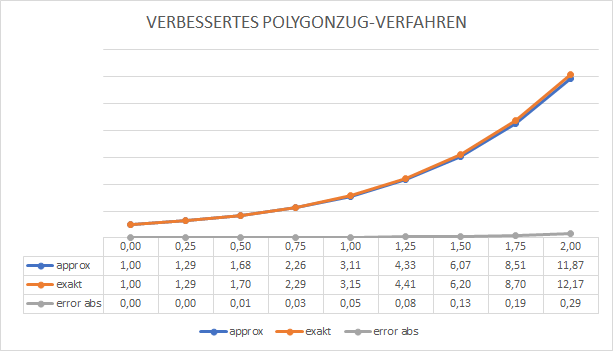
\includegraphics[width=0.7\textwidth]{../Mathematik_2/Bilder/eulerverfahren_verbesserter_polygonzug.png}
\end{center}
	\item[(c)]
	\begin{center}
	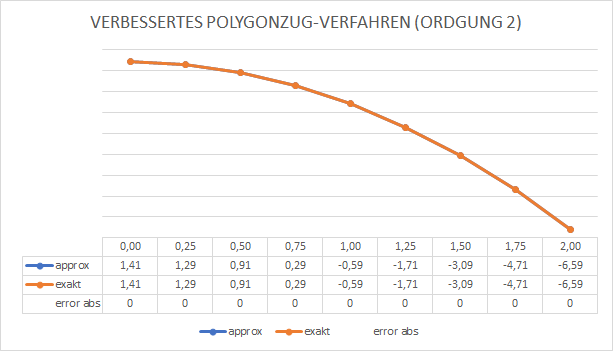
\includegraphics[width=0.7\textwidth]{../Mathematik_2/Bilder/eulerverfahren_verbesserter_polygonzug_zweite_ordnung.png}
\end{center}
		Das Verfahren scheint von der Ordnung zwei zu sein, das hei�t exakte L�sungen maximalem polynomialem Grad zwei werden exakt reproduziert!
\end{itemize}
\end{exercisebox}

\begin{exercisebox}[Explizites Euler Verfahren] %HMI 3 Blatt 7 Aufg. 3
	Betrachten Sie ein explizites Euler-Verfahren f�r das Anfangswertproblem
	\[
		\begin{cases}
			y(0) = 0\,,\quad & x=0\,,\\
			y' = 4x^2-7x+3\,,\quad & x\not=0\,.
		\end{cases}
	\]
	\begin{itemize}
		\item[(a)] Berechnen Sie die exakte L�sung  $\Phi$ des Anfangswertproblems.
		\item[(b)] Berechnen Sie bei vorgegebener Schrittweite $h$ mit dem Euler-Verfahren N�herungswerte $y_k$ f�r $\Phi(x_k)$ und explizit die Fehler $\epsilon(x_k,h) = y_k - \Phi(x_k)$ mit $x_k = kh$.
		\item[(c)] Zeigen Sie, dass der Fehler $\epsilon(x_k,h) = y_k - \Phi(x_k)$ bei festem $x$ f�r $h\to 0$ gegen Null konvergiert.
	\end{itemize}
\vspace{0.3cm}
\textbf{L�sung:} \newline
\begin{itemize}
		\item[(a)] Die exakte L�sung des Anfangswertproblems lautet \[ \Phi(x) = \frac43 x^3 - \frac72 x^2 + 3x \]
		\item[(b)] Um einen Ausdruck f�r den Fehler zu berechnen, ermitteln wir die St�tzstelle \(y_k\). Am effizientesten ist es die St�tzstellen f�r \(k=1,2,3\) explizit auszurechnen und dann eine Formel f�r beliebiges \(k\) herzuleiten (mathematisch pr�zise ist diese Formel dann mit einer vollst�ndigen Induktion zu beweisen - darauf verzichten wir hier).
			\begin{eqnarray*}
				y_0 &=& = 3h\\
				y_1 &=& = 3h + h ( 4 h^2-7h+3) = 4h^3 - 7h^2 + 6 h\\
				\cdots &=& \cdots \\
				y_k &=& y_{k-1} + h f(x_{k-1}, y_{k-1}) = 3(k+1)h + 4 h^3 \sum\limits_{i=0}^k i^2 - 7 h^2\sum\limits_{i=0}^k i
			\end{eqnarray*}
			Damit ergibt sich der Fehler
			\begin{eqnarray*}
				\epsilon(x_k, h) &=& y_k - \Phi(x_k) \\
				&=&  3(k+1)h + 4 h^3 \sum\limits_{i=0}^k i^2 - 7 h^2\sum\limits_{i=0}^k i -\frac43 k^3 h^3 - \frac72 k^2h^2 + 3kh \\
			&=& 3h + 2 h^3k^2 + \frac23h^3k-\frac72 kh^2 \,.\end{eqnarray*}
		\item[(c)] Es gilt \[ \lim\limits_{h\to 0}\left(  3h + 2 h^3k^2 + \frac23h^3k-\frac72 kh^2\right) = 0 \,.\]
	\end{itemize}

\end{exercisebox}

\begin{exercisebox}[Implizites Euler Verfahren] %HMI 3 Blatt 7 Aufg. 1a
	Betrachten Sie das Anfangswertproblem
	\[
		\begin{cases}
			y(0) = y_0\,,\quad & x=0\,,\\
			y' = -2at\,,\quad & x\not=0\,.
		\end{cases}
	\]
	Bestimmen Sie f�r das implizite Eulerverfahren den lokalen Diskretisierungsfehler
	\[
		\tau(t,h) := \frac1h \left( y(t_{k+1}) - y_{k+1} \right)
	\]
\vspace{0.3cm}
\textbf{L�sung:} \newline
	\begin{enumerate}
		\item Exakte L�sung des Anfangswertproblems: \( y(t) =  -at^2 + y_0 \,.\)
		\item Implizites Eulerverfahren: \( y_{k+1} = y_k + h\cdot f(x_{k+1}, y_{k+1}) \)
		\item Also
			\begin{eqnarray*}
				\tau(t,h) &=& \frac1h \left( -a( t_k + h)^2 + y_0 - y_k - h(2a(t_k+h) \right) \\
					&=& \frac1h \left( -ah^2 + 2h^2 a\right) = a\cdot h\,.
				\end{eqnarray*}
			\end{enumerate}
\end{exercisebox}

%
 \newpage
% \setcounter{exercise}{0} \section*{Trennbare Differentialgleichungen: L�sungen}\label{MA2-trennbare-differentialgleichungen-loesungen}

\ifintegriereaufgaben Erkl�rungen und Beispiele, die zum Verst�ndnis der L�sungswege hilfreich sind, finden Sie im Skript\wennreferenzvorhanden{MA2-trennbare-differentialgleichungen}{ (Abschnitt \abschnittsverweis{MA2-trennbare-differentialgleichungen})}.\fi

\begin{exercisebox}[Trennung der Variablen] %Papula IV, Abschnitt 2, Aufgabe 4
L�sen Sie die folgenden Differentialgleichungen durch Trennung der Variablen:
\begin{eqnarray*}
	\begin{array}{ll}
		(a)\; y' = \displaystyle{\frac{y^2}{x^2}}, \; x\in (0,\infty) \quad \quad & (b)\; y'= \displaystyle{\frac{x\cdot y}{1+x^2}} \\
			(c)\; y' = (1-y)^2 \quad \quad & (d)\; y'\cdot \sin(y)= -x,  \; y\in (0,\pi)
		\end{array}
\end{eqnarray*}
\vspace{0.3cm}
\textbf{L�sung:} \newline
Diese Aufgabe entspricht Aufg. \(4\) in dem Lehrbuch Papula Band 2, Abschnitt IV.2 zu finden auf Seite \(520\) und die L�sungen zu den Teilaufgaben finden Sie auf Seite \(726\).
\begin{itemize}
	\item[(a)] $y(x) = \displaystyle{\frac{x}{1+cx}} $
	\item[(b)] $y(x) = \displaystyle{c\cdot \sqrt{1+x^2}} $
	\item[(c)] $y(x) = \displaystyle{\frac{x+c-1}{x+c}} $
	\item[(d)] $y(x) = \mathrm{arccos}(x^2/2+c) $
\end{itemize}
\end{exercisebox}

\begin{exercisebox}[Inhomogenit�t] %Papula IV, Abschnitt 2, Aufgabe 16
	L�sen Sie folgenden Anfangswertprobleme durch Variation der Konstanten:
\begin{eqnarray*}
	\begin{array}{l c l}
		(a) \quad  xy'-y = x^2 \cdot \cos(x)  & \land & y(\pi) = 2\pi \\[1ex]
		(b) \quad  xy'+y = \ln(x) & \land & y(1) = 1\\[1ex]
		% (c) Papula \quad  y'+\tan(x)\cdot y = 5\cdot \sin(2x)  & \land & y(3\pi) = 2 \\[1ex]
		(c) \quad  y'-\tan(x)\cdot y = 5\cdot \sin(2x)  & \land & y(3\pi) = 2 \\[1ex] % Ver�nderung
	\end{array}
\end{eqnarray*}
\vspace{0.3cm}
\textbf{L�sung:} \newline
Diese Aufgabe entspricht bis auf Aufgabenteil (c) Aufg. \(16\) in dem Lehrbuch Papula Band 2, Abschnitt IV.2 zu finden auf Seite \(523\). Detaillierte L�sungen finden Sie ab Seite \(729\).
\begin{itemize}
	\item[(a)] $y(x) = 2x + x \cdot \sin(x) $
	\item[(b)] Papula $y(x) = 2/x+\ln(x) - 1$
	%\item[(c)] Papula $y(x) = -12\cdot \cos(x) - 10\cdot (\cos(x))^2$
		(c)
		\noindent{
			\hspace{-1cm}\begin{enumerate}
			\item Bestimmung der allgemeinen L�sung der homogenen Gleichung mit Trennung der Variablen: \[ y' - \tan(x) y = 0 \; \stackrel{y>0}{\Leftrightarrow} \; \dfrac{y'}{y} = \tan(x)  \; \Rightarrow \; \ln|y| = \ln\left( \Big| \dfrac{1}{\cos(x)}\Big|\right) + c \Rightarrow y_h(x) = \dfrac{\tilde c}{\cos(x)} \,.\]
			\item Bestimmung einer partikul�ren L�sung durch Variation der Konstante: \begin{eqnarray*}&& \begin{cases} y_p(x) &= c(x) \dfrac{1}{\cos(x) } \,,\\ y'_p(x) &= c'(x) \dfrac{1}{\cos(x)} + c(x) \tan(x)\dfrac{1}{\cos(x)}\,,\end{cases} \\ \stackrel{(A+E)}{\Rightarrow} && c(x) = 5\int \sin(2x) \cos(x)\,\mathrm{d} x \stackrel{ (*)}{=} -\dfrac{10}{3} \cos^3(x) \,,\end{eqnarray*}
			wobei das Integral \( (*)\)  mit Hilfe des Additionstheorems \(\sin(2x) = 2 \sin(x) \cos(x) \) gel�st wurde - im Detail \[ \int \sin(2x) \cos(x)\,\mathrm{d}x = 2\int \sin(x) \cos^2(x) \,\mathrm{d} x = -\dfrac{2}{3} \cos^3(x) + C \,.\]
		\item Bestimmung der allgemeinen L�sung der inhomogenen Gleichung durch Superposition: \[ y(x) = y_h(x) + y_p(x) = c\dfrac{1}{\cos(x)} - \dfrac{10}{3}\cos^3(x) \,. \]
		\item Bestimmung der speziellen L�sung des Anfangswertproblems durch Bestimmung der Konstante \(c\): \[ \cos(3\pi) = -1 \Rightarrow y(3\pi) = c\dfrac{1}{\cos(3\pi)} - \dfrac{10}{3}\cos^2(3\pi) = -c - \dfrac{10}{3} \stackrel{!}{=} 2 \Rightarrow c = -\dfrac{16}{3}\,.\]
	\end{enumerate}
}
\end{itemize}
\end{exercisebox}

\begin{exercisebox}[Substitution] %Papula IV, Abschnitt 2, Aufgabe 3
	L�sen Sie das folgende Anfangswertproblem:
	$
	y' = \displaystyle{\frac{y}{x} } +\displaystyle{\frac{x}{y} }, \quad y(1) = \sqrt{2}\,.
	$

\vspace{0.3cm}
\textbf{L�sung:} \newline
Diese Aufgabe entspricht Aufg. \(3\) in dem Lehrbuch Papula Band 2, Abschnitt IV.2 zu finden auf Seite \(520\) und die L�sung finden Sie auf Seite \(726\).

\vspace{0.3cm}
Die Differentialgleichung hat die Form \[ y' = f\left( \frac{y}{x}\right)\,.\] Die Idee ist die Substitution $u=y/x$ durchzuf�hren und eine Differentialgleichung mit trennbaren Variablen bzgl. \(u\) herzuleiten:
\begin{enumerate}
	\item Die Substitution f�hrt auf den folgenden Ausdruck f�r \(y'\)
\begin{eqnarray*}
	u=\frac{y}{x} \Rightarrow y = u\cdot x \Rightarrow y' = u'\cdot x + u
\end{eqnarray*}
\item Damit lautet die Differentialgleichung bzgl. \(u\)
	\begin{eqnarray*}
		u' \cdot x + u = u + \frac1u \Rightarrow u\cdot u' = \frac1x
	\end{eqnarray*}
\item Dies ist eine Differentialgleichung bzgl. \(u\), die sich durch Trennung der Variablen l�sen l��t:
	\[
\begin{aligned}
\int u\,\mathrm du &= \int\frac1x\,\mathrm dx
&&\Rightarrow\quad \frac12u^2(x)=\ln|x|+c,\\
u(x)&=\pm\sqrt{2\ln|x|+2c},\\
y(x)&=x\,u(x)=\pm x\sqrt{2\ln|x|+2c}.
\end{aligned}
\]
\item Die Integrationskonstante \(c\) ist durch die Bedingung $y(1) = \sqrt{2}$ bestimmbar:
	\[y(1) = 1\cdot \sqrt{2\ln|1| + 2c} = \sqrt{2c} \stackrel{!}{=} \sqrt{2} \Rightarrow c=1\,.\,. \]
\item Die eindeutige L�sung des Anfangswertproblem lautet:  \[ y(x) = x\sqrt{2 (\ln|x| + 1) }= x\sqrt{2 (\ln|x| + \ln(e)) }= x\sqrt{2\ln|ex|} \]
	\end{enumerate}
\end{exercisebox}

\begin{exercisebox}[Substitution] %Papula IV, Abschnitt 2, Aufgabe 2
	L�sen Sie die folgenden Differentialgleichungen mit Hilfe einer geeigneten Substitution. Schlagen Sie die auftretenden Integrale gegebenenfalls in einer Formelsammlung nach:
\begin{eqnarray*}
	\begin{array}{ll}
		(a)\; y' = \displaystyle{\frac{y}{x} + 4}, \; x\in (0,\infty) \quad \quad & (b)\; y'= (x+y+1)^2 \\
		(c)\; y' = \displaystyle{\frac14} + \displaystyle{\frac{y^2}{x^2}}, x\in (0,\infty) \quad \quad & (d)\; y' = \sin(\frac{y}{x}) + \frac{y}{x},  \; x\in (0,\infty)
		\end{array}
\end{eqnarray*}

\vspace{0.3cm}
\textbf{L�sung:} \newline
Diese Aufgabe entspricht Aufg. \(2\) in dem Lehrbuch Papula Band 2, Abschnitt IV.2 zu finden auf Seite \(520\) und die L�sungen finden Sie auf Seite \(726\).
\begin{itemize}
	\item[(a)] Substitution $ u=y/x \; \Rightarrow y(x) = cx +4x \ln(x) $
	\item[(b)] Substitution $ u=x+y+1 \; \Rightarrow y(x) = \tan(x+c) -x - 1$
	\item[(c)] Substitution $ u=y/x \; \Rightarrow y(x) = \displaystyle{\frac12} x - \displaystyle{\frac{x}{\ln|x|+\tilde c}} = \displaystyle{\frac12} x - \displaystyle{\frac{x}{\ln|\tilde c x|}} $ (\(ln\) bijektiv auf \(\mathbb R\) )
	\item[(d)] Substitution $ u=y/x \; \Rightarrow y(x) = 2\,x \cdot \mathrm{arctan}(cx) $
\end{itemize}
\end{exercisebox}

\begin{exercisebox}[Logistisches Wachstum]
	Die Anzahl der von einem Virus infizierten Personen $x(t)$ zum Zeitpunkt $t$ in einer Bev�lkerung der Gr��e $N$ kann folgenderma�en modelliert werden: Pro Tag habe jede Person $k>0$ zuf�llige Kontakte, wobei der Virus bei jedem Kontakt �bertragen wird. Stellen Sie eine Differentialgleichung auf und ermitteln Sie die L�sung. Wie lautet die L�sung des zugeh�rigen Anfangswertproblemes wenn $x(0)=1$ war?

Gehen Sie Schritt f�r Schritt vor:
	\begin{itemize}
		\item[(a)] Wie viele nicht infizierte Personen gibt es in Abh�ngigkeit von $x(t)$ zum Zeitpunkt $t$? Wie gro� ist der Anteil der nicht infizierten Personen zum Zeitpunkt $t$?
		\item[(b)] Wie viele Personen trifft eine infizierte Person in einer kleinen Zeitpanne $[t, t+\Delta t]$? Wieviele nicht infizierte Personen trifft eine infizierte Person in $[t, t+\Delta t]$?
		\item[(c)] Wie viele Kontakte von infizierten Personen mit nicht infizierten Personen gibt es insgesamt in $[t,t+\Delta t]$? Wie viele Personen werden daher in $[t, t+\Delta t]$ neu angesteckt?
		\item[(d)] Dr�cken Sie $x(t+\Delta t)$ durch $x(t)$ und die Anzahl der neu infizierten Personen in $[t, t+\Delta t]$ aus.
	\item[(e)] F�hren Sie den Grenzwert $\Delta t\to 0$ aus, um eine Differentialgleichung zu erhalten.
\end{itemize}
\vspace{0.3cm}
\textbf{L�sung:} \newline
\begin{itemize}
	\item[(a)] $N-x(t), \; (N-x(t))/N $
	\item[(b)] $k\cdot \Delta t, \; k\cdot (N-x(t))/N \cdot \Delta t $
	\item[(c)] $x(t) \cdot k \cdot (N-x(t))/N\cdot \Delta t $
	\item[(d)] $x(t+\Delta t) = x(t) + x(t) \cdot k \cdot (N-x(t))/N\cdot \Delta t $
	\item[(e)] \[ \frac{x(t+\Delta t) - x(t)}{\Delta t} = x(t)\cdot  k \cdot (N-x(t))/N  \stackrel{\Delta t\to 0}{\to} \dot x = k\cdot x(N-x)/N \]
		L�sung durch Trennung der Variablen
		\[ \int \frac{1}{x(N-x)} \, \mathrm{d}x = \int \frac{k}{N}\,\mathrm{d}t \]
		Integration durch Partialbruchzerlegung
		\[ \int\frac{1}{x(N-x)} \, \mathrm{d}x = \int\left( \frac{1}{N\cdot x} - \frac{1}{N\cdot (N-x)} \right) \,\mathrm{d}x = \frac1N \left( \log(x) - \log(N-x)\right) = \frac1N \log\left( \frac{x}{N-x}\right) \]
		Also
		\[ \log\left( \frac{x}{N-x}\right) = k\cdot t + c \Leftrightarrow \frac{x}{N-x} = c\cdot e^{kt} \Leftrightarrow x(t) = N\cdot \frac{c\cdot e^{kt}}{1+c\cdot e^{kt}} \]
		L�sung des Anfangswertproblems $x$ mit $c= \frac{1}{n-1}$.
\end{itemize}
\end{exercisebox}

\begin{exercisebox}[Differentialgleichungen erster Ordnung] %Papula IV, Abschnitt 2, Aufgabe 20
	L�sen Sie folgenden Differentialgleichungen mit Hilfe einer geeigneten Methode:
\begin{eqnarray*}
	\begin{array}{ll l }
		(a)\; y' = x(y^2+1) \;  & (b)\; y'= y\cdot \sin(x) \; & (c)\; y' = xy \\
		(d)\; xy' + y = 2\ln(x) \; (e)\; y' = 5x^4(y+1) \; & (f)\; y' - 5y = 2\cos(x) - \sin(3x)
		\end{array}
\end{eqnarray*}
\vspace{0.3cm}
\textbf{L�sung:} \newline
Diese Aufgabe entspricht Aufg. \(20\) in dem Lehrbuch Papula Band 2, Abschnitt IV.2 zu finden auf Seite \(523\) und L�sungen finden Sie auf Seite \(730\).
\begin{itemize}
	\item[(a)] Trennung der Variablen: \( y= \tan\left(\displaystyle{ \frac12} x^2 + c\right) \)
	\item[(b)] Trennung der Variablen: \( y= c\cdot e^{-\cos(x)} \)
	\item[(c)] Trennung der Variablen: \( y= c\cdot e^{\frac12 x^2} \)
	\item[(d)] Variation der Konstanten: \( y= 2(\ln(x) -1 ) + \frac{c}{2} \)
	\item[(e)] Trennung der Variablen: \( y= c\cdot e^{x^5} -1 \)
	\item[(f)] Ansatz vom Typ der rechten Seite: \( y= c\cdot e^{5x} + \frac1{13} \sin(x) - \frac{5}{13}\cos(x) + \frac{5}{34}\sin(3x) + \frac{3}{34} \cos(3x) \)
\end{itemize}
\end{exercisebox}

 \newpage
%
% \setcounter{exercise}{0} \section*{Laplace Transformation Aufgaben mit L�sungen}\label{MA2-laplacetransformation-loesungen}

\ifintegriereaufgaben Erkl�rungen und Beispiele, die zum Verst�ndnis der L�sungswege hilfreich sind, finden Sie im Skript\wennreferenzvorhanden{MA2-laplacetransformation}{ (Abschnitt \abschnittsverweis{MA2-laplacetransformation})}. \fi

\begin{exercisebox}[Uneigentliche Integrale] %A.Z. Integralrechnung  % Papula I.V, Abschnitt 9, Aufgabe 1 und 2
	Bestimmen Sie den Wert der folgenden uneigentlichen Integrale, falls er existiert.
	\begin{eqnarray*}
		(a)\;\int_0^\infty e^{-x}\,\mathrm{d}x\quad
		(b)\;\int_0^\infty x\cdot e^{-x}\,\mathrm{d}x\quad
		(c)\;\int_{-\infty}^2 e^{x}\,\mathrm{d}x\quad
		(d)\;\int_{0}^\infty x^2\cdot e^{-2x}\,\mathrm{d}x
	\end{eqnarray*}
\vspace{0.3cm}
\textbf{L�sung:} \newline
Diese Aufgaben entsprechen den Aufgaben \(1\) und \(2\) zu Abschnitt V.\(9\) in Papula Band 1. Die Aufgabenstellungen finden Sie auf Seite \(564\) und detaillierte L�sungswege auf Seite \(798\).
\begin{itemize}
	\item[(a)] Papula 1.V.9, Aufg. 1.a) $\quad 1$
	\item[(b)] Papula 1.V.9, Aufg. 1.b) $\quad 1$
	\item[(c)] Papula 1.V.9, Aufg. 1.c) $\quad e^2$
	\item[(d)] Papula 1.V.9, Aufg. 2) $\quad 1/4$
\end{itemize}
\end{exercisebox}

\begin{exercisebox}[Uneigentliche Integrale] %A.Z. Integralrechnung  % Papula I.V, Abschnitt 9, Aufgabe 4
	Bestimmen Sie den Wert der folgenden uneigentlichen Integrale, falls er existiert.
	\begin{eqnarray*}
		(a)\;\int_{-1}^0 \frac{1}{\sqrt{1+x}}\,\mathrm{d}x\quad
		(b)\;\int_{-1}^{1} \frac{1}{x^2}\,\mathrm{d}x\quad
		(c)\;\int_{0}^{10} \frac{e^{x}}{e^x-1}\,\mathrm{d}x
	\end{eqnarray*}
\vspace{0.3cm}
\textbf{L�sung:} \newline
Diese Aufgabe entspricht Aufgabe \(4\) zu Abschnitt V.\(9\) in Papula Band 1. Die Aufgabenstellungen finden Sie auf Seite \(565\) und detaillierte L�sungswege auf Seite \(799\).
\begin{itemize}
	\item[(a)] $2$
	\item[(b)] divergent
	\item[(c)] divergent
\end{itemize}
\end{exercisebox}


\begin{exercisebox}[Laplace-Transformation] % Papula II VI, Abschnitt 1, Aufgabe 1 und 3
	Aufgabe war es zu den gegebenen Funktionen die Laplace-Transformierte durch explizite Berechnung zu bestimmen. Die Aufgaben finden Sie im Lehrbuch von Papula Band II, Abschnitt VI.\(1\) auf Seite \(676\) und detaillierte L�sungswege auf Seite \(766\):
	\begin{itemize}
	\item[(a)] Papula, Aufg. 1.b)  $\quad f(t) = 2t\cdot e^{-4t}$
	\item[(b)] Papula, Aufg. 1.c)  $\quad f(t) = e^{-\delta t} \cdot \sin(\omega t), \; \delta, \omega >0$
	\item[(c)] Papula, Aufg. 1.d)  $\quad f(t) = \mathrm{sinh}(at),\, a>0$
	\item[(d)] Papula, Aufg. 1.f)  $\quad f(t) = \sin^2(t)$
\item[(e)] Papula, Aufg. 3.a) \(\quad\) (Rechteckimpuls) F�r $a>0$
			\[ f(t) = \begin{cases} A, \quad & 0<t<a\,,\\
					-A, \quad & a< t < 2a\,,\\
			0, \quad \mathrm{sonst}\,. \end{cases}\]
		\item[(f)] Papula, Aufg. 3.b) \(\quad\) (Sinusimpuls) F�r $a>0$
			\[ f(t) = \begin{cases} A\cdot \sin\left( \frac{\pi\cdot t}{a}\right), \quad & 0\leq t \leq a\,,\\
			0, \quad \mathrm{sonst}\,. \end{cases}\]
	\end{itemize}
\end{exercisebox}


\begin{exercisebox}[Laplace-Transformation] % Papula II, VI, Abschnitt 2, Aufgabe 4
	Bestimmen Sie
	%mit Hilfe von
	%\[ \sin(t) \laplace \frac{1}{s^2+1} \]
	die Laplace-Transformierte von
	\[ f(t) = \sin(\omega t + \varphi), \; \omega,\varphi >0\,. \]
	%indem Sie zuerst eine Verschiebung und dann eine Skalierung verwenden.

\vspace{0.3cm}
\textbf{L�sung:} \newline
		\begin{eqnarray*}
	I &=& \int\limits_0^\infty \sin(\omega t +\varphi) e^{-st}\,\mathrm{d}t = \frac{1}{s}\sin(\varphi) + \frac{\omega}{s} \int\limits_{0}^\infty \cos(\omega t+\varphi) e^{-st}\,\mathrm{d}t \\ &=& \frac{1}{s}\sin(\varphi) + \frac{\omega}{s^2}\cos(\varphi) - \frac{\omega^2}{s^2} I  \\
	&\Rightarrow &  I \left( 1+\frac{\omega^2}{s^2}\right) = \frac1s\sin(\varphi) - \frac{\omega}{s^2}\cos(\varphi)
\end{eqnarray*}
Also erhalten wir
\[ \Rightarrow I = \mathcal L(f) = \frac{1}{s^2} \left( s \sin(\varphi) - \omega \cos(\varphi) \right)  \frac{s^2}{s^2 + \omega^2} = \frac{  s \sin(\varphi) - \omega \cos(\varphi)}{s^2 + \omega^2}\,.\]

Einen alternativen L�sungsweg, der von den S�tzen �ber die Laplace-Transformierte bei " Manipulationen vom Argument " (Beschleunigung und Verschiebung des Signals) Gebrauch macht, finden Sie im Lehrbuch von Papula Band II, Abschnitt VI.\(2\) finden Sie auf Seite \(767f\). Die Aufgabe ist Aufgabe \(4\) auf Seite \(678\).
\end{exercisebox}
 \newpage
% \setcounter{exercise}{0} \section*{Laplace Transformation Anwendungen Aufgaben mit L�sungen}\label{MA2-laplacetransformation-und-differentialgleichungen-loesungen}

\ifintegriereaufgaben Erkl�rungen und Beispiele, die zum Verst�ndnis der L�sungswege hilfreich sind, finden Sie im Skript\wennreferenzvorhanden{MA2-laplacetransformation-und-differentialgleichungen}{ (Abschnitt \abschnittsverweis{MA2-laplacetransformation-und-differentialgleichungen})}. \fi

\begin{exercisebox}[Laplace-Transformation Rechenregeln] % Papula 2, VI, Abschnitt 2, Aufgabe 1, 2, 3, 5, 6, 7, 9, 10
	Die Aufgaben finden Sie in Papula 2.VI.2 ab Seite \(677\) und die L�sungen ab Seite \(767\).
	\begin{itemize}
		\item[(a)] Papula, Aufg. 1a) $\quad \mathcal L_f(s) = \frac{24}{s^4} - \frac{2}{s^3} + \frac{2}{s^2} $
	\item[(b)] Papula, Aufg. 1.b) $\quad \mathcal L_f(s) = C\left(\frac1s - \frac{1}{s+\lambda}\right) $
\item[(c)] Papula, Aufg. 2.a) $\quad \mathcal L_f(s) = \frac{29160}{s^6} $
		\item[(d)] Papula, Aufg. 2.b) $\quad \mathcal L_f(s) = \frac{s}{s^2+16}$
	\item[(e)] Papula, Aufg. 2.d) $\quad \mathcal L_f(s) = \frac{s^2+2\omega^2}{s(s^2+4\omega^2)} $
\item[(f)] Papula, Aufg. 3.b) $\quad \mathcal L_f(s) = \frac{2\cdot e^{-4s}}{s^3} $
		\item[(g)] Papula, Aufg. 3.c) $\quad \mathcal L_f(s) = \frac{e^{-bs}}{s-1} $
	\item[(h)] Papula, Aufg. 3.a) $\quad \mathcal L_f(s) = \frac{s}{s^2+1} $ (Achtung: Verschiebungsformel nicht anwendbar, weil keine Verschiebung nach rechts vorliegt!)
\item[(i)] Papula, Aufg. 5.a) $\quad \mathcal L_f(s) = \frac{s-3}{(s-3)^2+4} $
\item[(j)] Papula, Aufg. 5.b) $\quad \mathcal L_f(s) = \frac{A\omega}{(s+\delta)^2+\omega^2} $
		\item[(k)] Papula, Aufg. 5.c) $\quad \mathcal L_f(s) = \frac{1}{s-3\ln(2)}$
		\end{itemize}
\end{exercisebox}


\begin{exercisebox}[Laplace-Transformation und Differentialgleichungen]
	Betrachten Sie die Differentialgleichung $ y'' + \omega^2 y = 0,\; \omega>0$ mit den beiden Anfangswerten
	\begin{enumerate}
		\item $y(0) = 1 \land y'(0) = 0$
		\item $y(0) = 0 \land y'(0) = 1$
	\end{enumerate}
	\begin{itemize}
		\item[(a)] Berechnen Sie die L�sung der beiden Anfangswertprobleme.
		\item[(b)] Berechnen Sie die Laplace-Transformierte $Y(s)$ der Differentialgleichung \( y'' + \omega^2\, y = 0\). Nutzen Sie dabei die Ableitungsregeln.
		\item[(c)] Bestimmen Sie, ausgehend von den speziellen L�sungen der Anfangswertprobleme im Bildbereich, die L�sungen im Zeitbereich. Verwenden Sie f�r die R�cktransformationen eine Tabelle.
	\end{itemize}
\vspace{0.3cm}
\textbf{L�sung:} \newline
	\begin{itemize}
		\item[(a)] Die L�sungen lauten
			\[y_1(t) = \cos(\omega t), \; y_2(t) = 1/\omega \cdot \sin(\omega t)\]
		\item[(b)] Laplace-Transformation
			\begin{eqnarray*}
				\mathcal L\left(y'' + \omega^2 y\right)(s) &=& \mathcal L\left(y''\right) (s) + \omega^2\mathcal L\left( y\right)(s) \\
				&=& s^2\mathcal L\left( y\right) (s) - s y(0) + \omega^2 \mathcal L\left( y\right) (s) \\
				&=& s^2 Y (s) - s y(0) - y'(0) + \omega^2 Y(s) \stackrel{!}{=} 0\,.
			\end{eqnarray*}
		\item[(c)] Erstes Anfangswertproblem
			\[ s^2 Y_1(s) - s+ \omega^2 Y_1(s) = 0 \Leftrightarrow Y_1(s) = \frac{s}{s^2+\omega^2} \Rightarrow y_1(t) = \cos(\omega t)\,.\]
		Zweites Anfangswertproblem
		\[ s^2 Y_2(s) - 1 + \omega^2 Y_2(s) = 0 \Leftrightarrow Y_2(s) = \frac{1}{s^2+\omega^2} \Rightarrow y_2(t) = \frac{1}{\omega}\cdot \sin(\omega t)\,.\]
\end{itemize}
\end{exercisebox}

\begin{exercisebox}[Laplace-Transformation und Differentialgleichungen]
	L�sen Sie die folgenden Systeme mit Hilfe der Laplace-Transformation
	\begin{eqnarray*}
		(a)\; \begin{cases}
			x(0) = y(0) =  0, \quad & t= 0\,,\\
			\dot x + 2 y = e^t, \quad & t> 0\,,\\
			\dot y + 2 x = e^{-t}, \quad & t> 0\,.
		\end{cases} \quad\quad
		(b)\; \begin{cases}
			x(0) = y(0) =  0, \quad & t= 0\,,\\
			\dot x(0) = \dot y(0) =  0, \quad & t= 0\,,\\
			\ddot x + \dot y + 3 y = 1, \quad & t> 0\,,\\
			\ddot y -4 \dot x + 3y = 0, \quad & t> 0\,.
		\end{cases} \quad\quad
	\end{eqnarray*}
\vspace{0.3cm}
\textbf{L�sung:} \newline
	\begin{itemize}
		\item[(a)]
			Anwendung der Laplace-Transformation und Einsetzen der Anfangsbedingungen ergibt:
			\[
		\begin{cases}
			s X(s) + 2 Y(s) = \displaystyle{\frac{1}{s-1}}\,,\\
			2 X(s) + sY(s) = \displaystyle{\frac{1}{s+1}}\,.
	\end{cases} \]

%			Und nach Einsetzen der homogenen Anfangsbedingungen erhalten wir das folgende lineare Gleichungssystem:
%			\[
%				\left( \begin{array}{cc} s & -2 \\ -2 & s\end{array}\right) \left( \begin{array}{c} X \\Y \end{array}\right)(s) = \frac{1}{s^2-1}\left( \begin{array}{c} s+1 \\ s-1 \end{array}\right) \,.
%\]
	Aufl�sen\footnote{ Entweder durch Einsetzen der Gleichungen ineinander oder durch Anwendung der inversen Matrix!} und Partialbruchzerlegung liefert
			\[
		\begin{cases}
			X(s) = \displaystyle{\frac{s^2 - s + 2}{(s^2-1)(s^2-4)}} = \displaystyle{\frac{1}{3}}\left( \displaystyle{\frac{2}{s+1}} - \displaystyle{\frac{1}{s-1}} - \displaystyle{\frac{2}{s+2}} + \displaystyle{\frac{1}{s-2}}\right)\,,\\
			Y(s) = \displaystyle{\frac{s^2 - 3s - 2}{(s^2-1)(s^2-4)}} = \displaystyle{\frac{1}{3}}\left( \displaystyle{\frac{1}{s+1}} + \displaystyle{\frac{2}{s-1}} - \displaystyle{\frac{2}{s+2}} - \displaystyle{\frac{1}{s-2}}\right)\,.
	\end{cases} \]
	R�cktransformation liefert die L�sung des Systems:
			\[
		\begin{cases}
			x(t) =  \displaystyle{\frac{1}{3}}\left( 2 e^{-t} - e^{t} - 2 e^{-2t} + e^{2t} \right)\,,\\
			y(t) =  \displaystyle{\frac{1}{3}}\left( e^{-t} +2 e^{t} - 2 e^{-2t} - e^{2t} \right)\,.
	\end{cases} \]

		\item[(b)]
			Laplace-Transformation des Systems unter Bere�cksichtigung der Anfangsbedingungen:
			\[
		\begin{cases}
			\left( s^2 + 3\right) X(s) + s Y(s) = \displaystyle{\frac{1}{s}}\,,\\
			-4s X(s) + \left( s^2 + 3\right) Y(s) = 0\,.
	\end{cases} \]
	Aufl�sen und Partialbruchzerlegung liefert
			\[
		\begin{cases}
		X(s) = \displaystyle{\frac{s^2 +3}{s(s^2+9)(s^2+1)}} =\displaystyle{\frac{1}{3 s}} - \displaystyle{\frac{1}{12(s^2+9)}} - \displaystyle{\frac{s}{4(s^2+1)}}\,,\\
	Y(s) = \displaystyle{\frac{4}{(s^2+9)(s^2+1)}} = -\displaystyle{\frac{1}{2(s^2+9)}} + \displaystyle{\frac{1}{2(s^2+1)}} \,.
	\end{cases} \]
	R�cktransformation liefert die L�sung des Systems:
			\[
		\begin{cases}
			x(t) =  \displaystyle{\frac{1}{3}}- \displaystyle{\frac{1}{12}}\cos(3t)-\frac14\cos(t)\,,\\
			y(t) =  -\displaystyle{\frac{1}{6}}\sin(3t) + \displaystyle{\frac12} \sin(t)\,.
	\end{cases} \]
	\end{itemize}
\end{exercisebox}

 \newpage
% \setcounter{exercise}{0} \section*{Partialbruchzerlegung Aufgaben mit L�sungen}\label{MA2-partialbruchzerlegung-loesungen}

\ifintegriereaufgaben Regeln und Beispiele, die zum Verst�ndnis der L�sungswege hilfreich sind, finden Sie im Skript\wennreferenzvorhanden{MA2-partialbruchzerlegung}{ (Abschnitt \abschnittsverweis{MA2-partialbruchzerlegung})}.\fi

\begin{exercisebox}[Faktorisierung]
	Zerlegen Sie die folgenden Polynome weitestgehend in {Linearfaktoren}.
	\begin{eqnarray*}
			(a)\;4y^3-8y^2-3y+9 \quad (b)\; a^4+3a^2-10 \quad (c) \; x^4+2x^3-35x^2  \quad (d)\; -64+b^2
	\end{eqnarray*}

\vspace{0.3cm}
\textbf{L�sung:} \newline
Erinnern Sie sich an die Standard-Tricks zum L�sen algebraischer Gleichungen:
\begin{enumerate}
	\item bei einem linearen Polynom ist die Vorgehensweise klar: Gleichung aufl�sen.
	\item bei einem quadratischen Polynom ist die Vorgehensweise klar: Gleichung aufl�sen (allgemeine L�sungsformel).
	\item machmal lassen sich gemeinsame Potenz von der Variable ausklammern und der Rest ist ein quadratisches Polynom, was mit der allgemeinen L�sungsformel zu behandeln ist.
	\item bei Polynomen, die nur gerade Potenzen von x aufweisen, bietet sich eine Substitution der Form \(x^2= y\), damit wird der Polynomgrad um zwei reduziert und Sie erh�lten im besten Fall ein quadratisches Polynom in \(y\) - hier ist die R�cksubstitution nicht zu vergessen!
	\item Binomische Formeln sollten Sie erkennen k�nnen.
	\item Wenn all das nicht hilft, hilft nur noch eine Nullstelle zu raten und da beginnen Sie mit \(x=1\), dann \(x=-1\) vielleicht noch \(x=2\) und \(x=-2\) und wenn da nichts zum Erfolg f�hrt, dann pr�fen Sie, ob Sie einen Abschreibfehler drin haben :)
	\end{enumerate}
So, jetzt geht es los:
\begin{itemize}
	\item[(a)] Fall \(6\) und \(y_1=-1\) ist eine Nullstelle! Also ist die Strategie: erst eine Polynomdivision (die muss ohne Rest aufgehen, sonst haben Sie einen Fehler gemacht!) und dann die allgemeine L�sungsformel f�r das Restpolnyom durchf�hren\ldots
		\begin{eqnarray*}
			\left( 4y^3 - 8y^2 -3y + 9\right) : \left( y+1\right) = 4y^2-12y+9 \Rightarrow y_{2,3} = \frac{12 \pm \sqrt{ 144 - 4 \cdot 4 \cdot 9 } }{ 2 \cdot 4 } = \frac32
			\end{eqnarray*}
			Die Linearfaktorzerlegung des Polnyoms lautet also
			\[4y^3 - 8y^2 -3y + 9 = 4 \cdot \left( y - \frac32\right)^2 \cdot \left( y+1\right)\]
			Vorsicht: denken Sie daran, dass die allgemeine L�sungsformel Ihnen die Nullstellen des Polynoms liefert - an den Faktor vor der h�chsten Potenz, im Beispiel \(4\), m�ssen Sie selbst denken, wenn eine �quivalente Darstellung des Polynoms gesucht ist!
		\item[(b)] Fall \(4\): setzen wir \(a^2 = x\), dann erhalten wir ein quadratisches Polynom in \(x\), dessen Nullstellen wir mit der allgemeinen L�sungsformel berechnen k�nnen:
			\begin{eqnarray*} a^4+3a^2-10 \Leftrightarrow a^2 = x \land x^2 + 3x-10 &=& ( x+5)\cdot( x-2),\\
			\textnormal{denn} \quad x_{1,2} &=& \frac{ -3 \pm \sqrt{ 9 -4\cdot 1 \cdot (-10)}}{2} = \begin{cases} -5 \\ 2 \end{cases}\end{eqnarray*}
				Die  R�cksubstitution liefert
				\[ a^4+3a^2 -10 = (a^2+5)\cdot (a^2-2) = (a-\sqrt{2})\cdot (a+\sqrt{2}) \cdot (a^2+5)\,, \]
				wobei der Faktor \( (a^2 - 2)\) in die Linearfaktoren \( (a-\sqrt{2}) \) und \( (a+\sqrt{2})\) zerlegt werden kann und der andere Faktor als quadratischer Term ohne reelle Nullstellen stehen bleiben muss.
			\item[(c)] Fall \(3\) tritt ein und wir erhalten
				\begin{eqnarray*} x^4+2x^3-35x^2 = x^2 \cdot ( x^2+2x-35) &=& x^2 \cdot (x-5)\cdot (x+7), \\ \mathrm{denn}\; x_{1,2} &=& \frac{-2\pm \sqrt{4-4\cdot 1 \cdot (-35)}}{2} = \frac{-2\pm 12}{2} = \begin{cases} -7 \\ 5\,.\end{cases} \end{eqnarray*}
				\item[(d)] Fall \(5\) (\(3\). Binomische Formel): \( -64+b^2 = (b+8)\cdot (b-8)\)
\end{itemize}
\end{exercisebox}

\begin{exercisebox}[Polynomdivision]
	F�hren Sie folgende {Polynomdivisionen} aus.
	\begin{eqnarray*}
		\begin{array}{l l }
			(a)\;(x^2+x):(x-1) \quad & (b)\; (x^3-x^2-x+1):(x-1) \\[2ex] (c) \; (x^3+x^2-5x+3) : (x-1)^2  \quad & (d)\; (x^4+x^3-2x) :(x-1)
		\end{array}
	\end{eqnarray*}

\vspace{0.3cm}
\textbf{L�sung:} \newline
\begin{itemize}
	\item[(a)] $(x^2+x):(x-1) = x+2 + \displaystyle{\frac{2}{x-1}} $
	\item[(b)] $(x^3-x^2-x+1):(x-1) = x^2-1$
	\item[(c)] $(x^3+x^2-5x+1):(x-1)^2 = x+3$
	\item[(d)] $(x^4+x^3-2x):(x-1) = x^3+2x^2+2x$
\end{itemize}
\end{exercisebox}
\begin{exercisebox}[Gau�-Algorithmus]
	L�sen Sie die folgenden Gleichungsysteme:
	\begin{eqnarray*}
		(a)\; \left\{ \begin{array}{cccccrcl}
	 &A_1 &  &      & + & B_2 & =& 0 \\
	 &4A_1& +& 4A_2 & + & 2B_2& =& -2 \\
	 &4A_1&- & 2A_2 & + & 8B_2& =& -38
 \end{array} \right.\quad \quad
		(b)\;  \left\{ \begin{array}{crcrcrcl}
	 -&x & + & y & +& z &=& 0 \\
	 &x & -&3y & -&2z & =& 5 \\
	 &5x & +&y & +&z &=& -6
 \end{array} \right.
 \end{eqnarray*}
\vspace{0.3cm}
\textbf{L�sung:} \newline
L�sung durch Anwendung des Gau�-Algorthmus, das hei�t die erweiterte Matrix wird auf Trapezform gebracht und das Gleichungssystem wird von unten nach oben gel�st:
\begin{itemize}
       	 \item[(a)]
 \begin{eqnarray*}
	 &&\left( \begin{array}{ccc|c} 1 & 0 & 1 & 0 \\ 4 & 4 & 2 & -2 \\ 4 & -2 & 8 & -38 \end{array}\right) \Leftrightarrow  \left( \begin{array}{ccc|c} 1 & 0 & 1 & 0 \\ 2 & 2 & 1 & -1 \\ 2 & -1 & 4 & -19 \end{array}\right) \\\Leftrightarrow &&  \left( \begin{array}{ccc|c} 1 & 0 & 1 & 0 \\ 0 & 2 & -1 & -1 \\ 0 & 0 & 3 & -39 \end{array}\right) \Rightarrow  \begin{cases} A_1 &= 13 \\ A_2 & = -7 \\ B_2 &= -13 \end{cases}
 \end{eqnarray*}
       	 \item[(b)]
 \begin{eqnarray*}
	 &&\left( \begin{array}{ccc|c} -1 & 1 & 1 & 0 \\ 1 & -3 & -2 & 5 \\ 5 & 1 & 1 & -6 \end{array}\right) \Leftrightarrow  \left( \begin{array}{ccc|c} -1 & 1 & 1 & 0 \\ 0 & -2 & -1 & 5 \\ 0 & 1 & 1 & -1 \end{array}\right) \\\Leftrightarrow &&  \left( \begin{array}{ccc|c} -1 & 1 & 1 & 0 \\ 0 & -2 & -1 & 5 \\ 0 & 0 & 1 & 3 \end{array}\right) \Rightarrow  \begin{cases} x &= -1 \\ y & = -4 \\ z &= 3 \end{cases}
 \end{eqnarray*}
\end{itemize}
\end{exercisebox}

\begin{exercisebox}[Partialbruchzerlegung]
	F�hren Sie eine Partialbruchzerlegung durch.
	\begin{eqnarray*}
		(a)\; \frac{2x^3-x^2-6x+2}{(x-5)^2(x^2+3x+4)} \quad\quad (b)\; \displaystyle{ \frac{x+1}{x(x^2+1)^2}}
\quad & (d)\; \displaystyle{\frac{x^2-5x}{(x-2)^3}}
		\end{eqnarray*}

\vspace{0.3cm}
\textbf{L�sung:} \newline
Die Nennerpolynome der gebrochenrationalen Ausdr�cke liegen schon in faktorisierter Form vor und der Quotient ist vollst�ndig gek�rzt. Die Partialbruchzerlegung startet also mit dem Ansatz f�r die Zerlegung.
  \begin{itemize}
	  \item[(a)] Der Ansatz lautet:
  \[
  \frac{2x^3-x^2-6x+2}{(x-5)^2(x^2+3x+4)} = \frac{A}{ (x-5)^2 } + \frac{B}{x-5 } + \frac{Cx+D}{x^2+3x+4 }\,.
  \]
Um die vier Konstanten $A$ bis $D$ zu bestimmen, fasst man das wieder zu einem Bruch zusammen:
  \[
\frac{2x^3-x^2-6x+2}{(x-5)^2(x^2+3x+4)} = \frac{A  (x^2+3x+4) + B (x-5) (x^2+3x+4) +( Cx+D) (x-5)^2}{(x-5)^2(x^2+3x+4)}
  \]

Also muss f�r die Z�hler gelten:
\[ 2x^3-x^2-6x+2 \stackrel{!}{=} A  (x^2+3x+4) + B (x-5) (x^2+3x+4) +( Cx+D) (x-5)^2\,. \]

Das muss f�r alle reellen Zahlen $x$ gelten. Daraus muss man nun vier Gleichungen f�r die vier Konstanten $A$ bis $D$ basteln. Daf�r gibt es zwei Wege:
\begin{itemize}
  \item Verschiedene Werte f�r $x$ einsetzen: Zum Beispiel findet man f�r $x=5$
  \[
  2 \cdot 125- 25 -30+2 \stackrel{!}{=} A (25+15+4) \,.
  \]

\item Links und rechts Potenzen von $x$ zusammenfassen und einen Koeffizientenvergleich machen: Zum Beispiel steht links $2x^3$ und rechts
\[
	2x^3 \stackrel{!}{=} (B+C) x^3  \Rightarrow B+C\stackrel{!}{=} 2\,.
  \]
\end{itemize}
\item[(b)]
 Der Ansatz f�r die Partialbruchzerlegung lautet
		\[ \frac{x+1}{x(x^2+1)^2} = \frac{A_1}{x} + \frac{B_1x+C_1}{x^2+1} +  \frac{B_2x+C_2}{(x^2+1)^2}\,. \]
		Ein Koeffizientenvergleich f�hrt auf das Gleichungssystem zur Bestimmung des Vektors $(A_1, B_1, B_2, C_1, C_2)^\intercal$
		\begin{eqnarray*}
			\left( \begin{array}{ccccc|c } 1 & 1 & 0 & 0 & 0 & 0 \\
					0 & 0 & 0 & 1 & 0 & 0 \\
					2 & 1 & 1 & 0 & 0 & 0 \\
					0 & 0 & 0 & 1 & 1 & 1 \\
			1 & 0 & 0 & 0 & 0 & 1 \end{array}\right) \Rightarrow A_1 = C_2 =  1, B_1 = B_2 = -1, C_1 = 0
		\end{eqnarray*}
 Die  Partialbruchzerlegung lautet
		\[
		\frac{x+1}{x(x^2+1)^2} = \frac{1}{x} - \frac{1}{x^2+1} -  \frac{x-1}{(x^2+1)^2}\,. \]
\item[(c)]
Der Ansatz lautet:
		\[ \frac{x^2-5x}{(x-2)^3} = \frac{A}{x-2} + \frac{B}{(x-2)^2} + \frac{C}{(x-2)^3} \]
 Die Partialbruchzerlegung ist:
		\[ \frac{x^2-5x}{(x-2)^3} = \frac{1}{x-2} - \frac{1}{(x-2)^2} - \frac{6}{(x-2)^3} \]
\end{itemize}
\end{exercisebox}


\begin{exercisebox}[Partialbruchzerlegung]
	F�hren Sie eine Partialbruchzerlegung durch. Hinweis: Die Nennerpolynome haben mindestens eine ganzzahlige Nullstellen.
	\begin{eqnarray*}
		\begin{array}{l l l }
			(a) \; \displaystyle{ \frac{1}{x^3+x}}  \quad\quad & (b)\; \displaystyle{ \frac{(4x^5-6x+13)(x-1)(x^2-1)}{x^3-x^2-x+1}} (c) \;  \displaystyle{ \frac{2x^2+x+1}{x^3+x^2-5x+3}} \\[2ex]
			(d)\; \displaystyle{ \frac{-x^4-2x^3+7x^2-5x+3}{ x^2+3x-4}} \quad\quad & (e)\; \displaystyle{ \frac{x^2+x+1}{x^3-3x+2}}
		\end{array}
	\end{eqnarray*}
\vspace{0.3cm}
\textbf{L�sung:} \newline
\begin{itemize}
	\item[(a)]
		Faktorisierung des Nennerpolynoms
		\[ x^3 + x = x(x^2+1) \]
		Partialbruchzerlegung
		\[ \frac{1}{x(x^2+1)} = \frac1x - \frac{x}{x^2+1} \]
\item[(b)]
	Die Faktorisierung des Nenners lautet $(x-1)(x^2-1)$, das Nennerpolynom l��t sich also komplett wegk�rzen und es ist nichts weiter zu tun:
	\[ \displaystyle{ \frac{(4x^5-6x+13)(x-1)(x^2-1)}{x^3-x^2-x+1}} = \frac{(4x^5-6x+13)(x-1)(x^2-1)}{(x^2-1)(x-1)} = 4x^5-6x+13\,.\]
\item[(c)]
	\begin{itemize}
		\item Die Faktorisierung des Nennerpolynoms lautet
	\[x^3+x^2-5x+3 = (x-1)^2\cdot (x+3)\]
\item Der Nenner besitzt also eine zweifache Nullstelle in $x=1$ und eine einfache Nullstelle in $x=-3$. Der Ansatz f�r die Partialbruchzerlegung lautet also
	\[
	\displaystyle{ \frac{2x^2+x+1}{(x-1)^2\cdot (x+3)} = \displaystyle{\frac{A_1}{x-1}} +  \displaystyle{\frac{A_2}{(x-1)^2}} +  \displaystyle{\frac{B_1}{x+3}}}\]
\item
	Ein Koeffizientenvergleich zwischen den Z�hlern beider Seiten f�hrt auf das folgende lineare Gleichungssystem f�r den Vektor $(A_1, A_2, B_1)^\intercal$
	\begin{eqnarray*}
		\left( \begin{array}{ccc |c}
				1 & 0 & 1  & 2 \\
				2 & 1 & -2 & 1\\
		-3 & 3 & 1  & 1 \end{array}\right) \Leftrightarrow
		\left( \begin{array}{ccc | c}
				1 & 0 & 1 & 2  \\
				0 & 1 & -4 & -3 \\
		0 & 0 & 16 & 16 \end{array}\right) \Rightarrow  A_1 = A_2 = B_1 = 1\,.
	\end{eqnarray*}
\item Die Partialbruchzerlegung gem�� unseres Ansatzes lautet
	\[
	\displaystyle{ \frac{2x^2+x+1}{x^3+x^2-5x+3}}  = \displaystyle{\frac{1}{x-1}} +  \displaystyle{\frac{1}{(x-1)^2}} +  \displaystyle{\frac{1}{x+3}}
	\]
	\end{itemize}
	\item[(d)]
		Polynomdivision
		\[ \frac{-x^4-2x^3+7x^2-5x+3}{ x^2+3x-4} = \frac{3-x}{x^2+3x-4} - x^2 +x \]
		Faktorisierung des Nennerpolynoms
		\[ x^2+3x-4 = (x-1)(x+4) \]
		Partialbruchzerlegung
		\[ \frac{3-x}{x^2+3x-4} = \frac{2}{5(x-1)} - \frac{7}{5(x+4)} \]
	\item[(e)]
		Faktorisierung des Nennerpolynoms
		\[ x^3-3x+2 = (x-1)^2(x+2) \]
		Partialbruchzerlegung
		\[ \frac{x^2+x+1}{(x-1)^2(x+2)} = \frac{1}{3(x+2)} + \frac{2}{3(x-1)} + \frac{1}{(x-1)^2} \]
\end{itemize}
\end{exercisebox}

\begin{exercisebox}[Partialbruchzerlegung]
% Papula Band 1, Kapitel V, Abschnitt 8, Aufgabe 7 Aufgabe Seite  563, L�sung Seite 793 ff
	F�hren Sie eine Partialbruchzerlegung durch.
	\begin{eqnarray*}
		\begin{array}{l l l}
			(a)\; \displaystyle{ \frac{1}{ x^2-a^2}}, \; a>0 \;  \quad \quad & (b)\; \displaystyle{ \frac{4x^3}{x^3+2x^2-x-2}} \quad\quad & (c) \; \displaystyle{ \frac{3z}{z^3-3z^2-4}} \\[2ex]
			(d)\; \displaystyle{\frac{4x-2}{x^2-2x-63}} \; & (e)\; \displaystyle{\frac{2x+1}{x^3-6x^2+9x} }  &
		\end{array}
	\end{eqnarray*}

\vspace{0.3cm}
\textbf{L�sung:} \newline
Detaillierte L�sungen zu dieser Aufgabe finden Sie in Papula, Band \(1\). Die Partialbruchzerlegungen sind Teil der Aufgabe \(7\) auf Seite \(563\) im Abschnitt V.\(8\). Den L�sungsweg finden Sie auf den Seiten \(793-794\).
\end{exercisebox}

\begin{exercisebox}[Anwendung Partialbruchzerlegung]
	Berechnen Sie folgende Integrale. Hinweis: Nutzen Sie die Ergebnsise aus der vorigen Aufgabe.
	\begin{eqnarray*}
		\begin{array}{l l l}
			(a)\; \displaystyle{ \int \frac{-x^4-2x^3+7x^2-5x+3}{ x^2+3x-4}} \, \mathrm{d}x \quad & (b)\; \displaystyle{\int \frac{x^2+x+1}{x^3-3x+2}}\,\mathrm{d}x  & (c) \; \displaystyle{\int \frac{1}{x^3+x}}\,\mathrm{d}x \\[1ex]
			(d)\; \displaystyle{\int \frac{x^2-5x}{(x-2)^3}} \,\mathrm{d}x &(e)\; \displaystyle{ \int \frac{1}{ x^2-a^2}} \, \mathrm{d}x, \; a>0 & (f)\; \displaystyle{\int \frac{4x^3}{x^3+2x^2-x-2}}\,\mathrm{d}x \\[2ex]
			(g) \; \displaystyle{\int \frac{3z}{z^3-3z^2-4}}\,\mathrm{d}x  & (h)\; \displaystyle{\int \frac{4x-2}{x^2-2x-63}}\, \mathrm{d}x \quad & (i)\; \displaystyle{\int \frac{2x+1}{x^3-6x^2+9x}}  \, \mathrm{d}x
		\end{array}
	\end{eqnarray*}
\vspace{0.3cm}
\textbf{L�sung:} \newline
Detaillierte L�sungen zu den Aufgabenteilen \((e) -(i)\) finden Sie in Papula, Band \(1\) auf Seite \(793\)ff.
\begin{itemize}
	\item[(a)] $ F(x) = - \displaystyle{\frac{7}{5}}\ln|x+4| - \displaystyle{\frac{x^3}{3}} + \displaystyle{\frac{x^2}{2}}  + \displaystyle{\frac{2}{5}} \ln|x-1| + c $
	\item[(b)] $ F(x) = \displaystyle{\frac{1}{3}} \ln|x+2| - \displaystyle{\frac{1}{x-1}} + \displaystyle{\frac{2}{3}}\ln|x-1| + c $
	\item[(c)] $ F(x) = -\displaystyle{\frac{1}{2}} \ln(x^2+2) + \ln|x| + c $
	\item[(d)] $ F(x) = \displaystyle{\frac{1}{x-2}} + \displaystyle{\frac{3}{(x-2)^2}} + \ln|x-2| c $
	\item[(e)] $ F(x) = \displaystyle{\frac{1}{2a}} \ln\Big| \displaystyle{\frac{x-a}{x+a}}\Big| + c $
	\item[(f)] $ F(x) = \displaystyle{\frac{2}{3}} \ln| x-1| + 2 \ln|x+1| - \displaystyle{\frac{32}{3}}\ln|x+2| + 4x + c $
	\item[(g)] $ F(x) = \displaystyle{\frac{1}{3}} \ln\Big| \displaystyle{\frac{z-1}{z+2}}\Big| - 2 \displaystyle{\frac{2}{z+2}} + c $
	\item[(h)] $ F(x) = \displaystyle{\frac{17}{8}} \ln|x-9| + \displaystyle{\frac{15}{8}}\ln|x+7| + c $
	\item[(i)] $ F(x) = \displaystyle{\frac{1}{9}} \ln\Big| \displaystyle{\frac{x}{x-3}}\Big| - \displaystyle{\frac{7}{3(x-3)}} + c $
\end{itemize}
\end{exercisebox}


 \newpage
% \setcounter{exercise}{0} \section*{Systemanalyse L�sungen}\label{MA2-systemanalyse-loesungen}

\ifintegriereaufgaben Regeln und Beispiele, die zur Bearbeitung der Aufgaben hilfreich sind, finden Sie im Skript\wennreferenzvorhanden{MA2-systemanalyse}{ (Abschnitt \abschnittsverweis{MA2-systemanalyse})}.\fi


\begin{exercisebox}[Polstellen (�bertragungsfunktion Laplace) ] % s=-1, s=-2
Gegeben sei

\[
	H(s)=\frac{2}{s^2+3s+2} = \frac{2}{(s+1)\cdot (s+2)}
\]


\begin{enumerate}

	\item Die Faktorisierung des Nennerpolynoms liefert die Polstellen \(s=-1\) und \(s=-2\)\,.
		\[ s_{1,2} = \dfrac{(-3) \pm \sqrt{ 3^2 - 4\cdot  2 }}{2} = \dfrac{-3 \pm 1}{2}  \Rightarrow \, H(s)=\frac{2}{s^2+3s+2} = \frac{2}{(s+1)\cdot (s+2)} \]

\item Skizzieren Sie die Lage der Polstellen in der komplexen Ebene:

\begin{center}
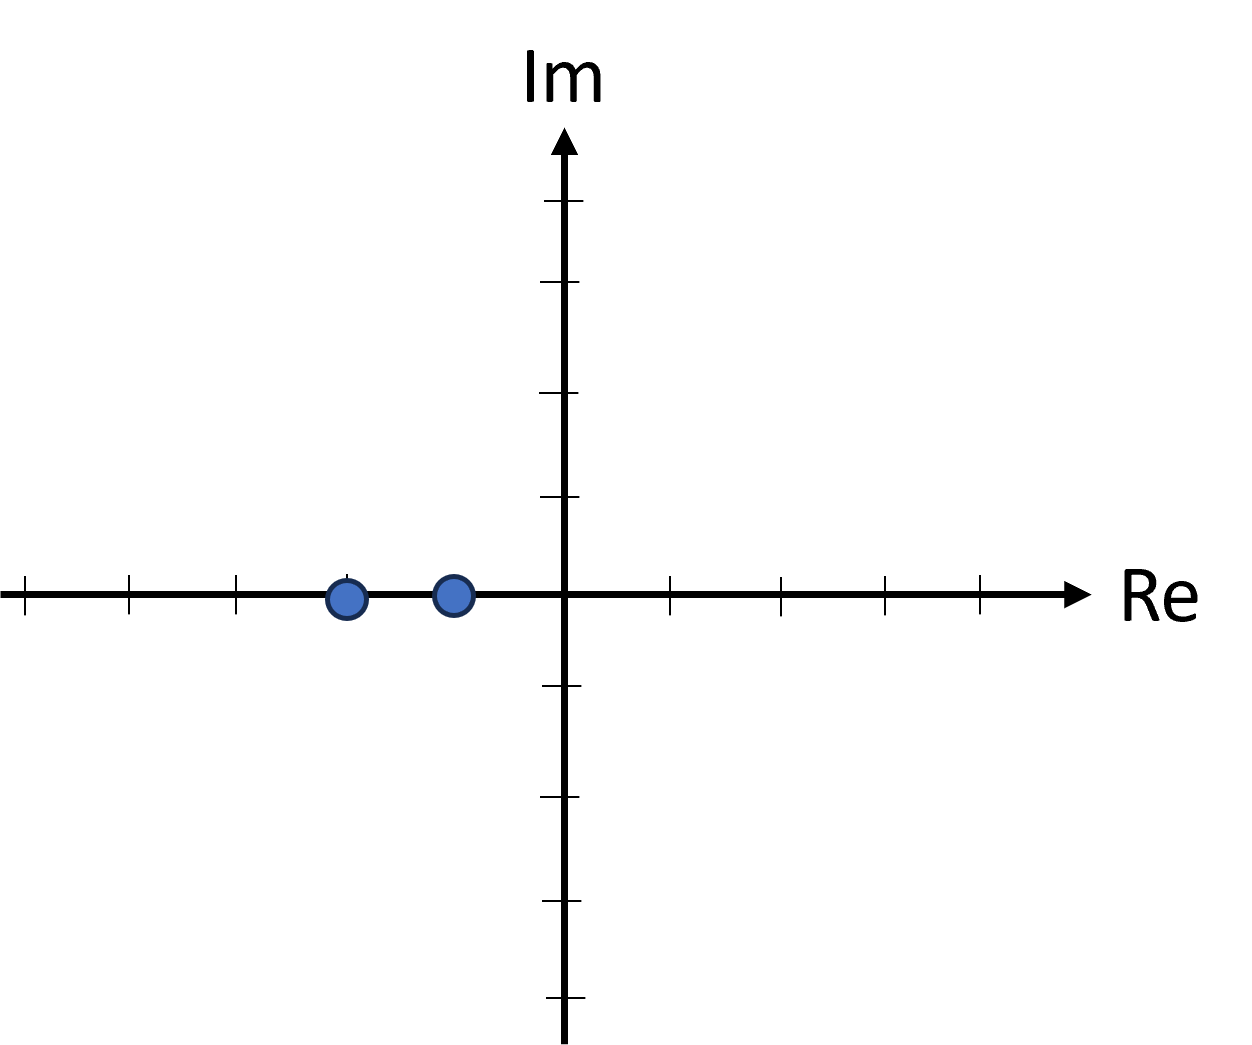
\includegraphics[width=5cm]{../Mathematik_2/Bilder/systemanalyse_reelle_polstellen.png}
\end{center}

\end{enumerate}


\end{exercisebox}

\begin{exercisebox}[Polstellen (�bertragungsfunktion Laplace)] % s = -1 pm 2i
Gegeben sei

\[
H(s)=\frac{1}{s^2+2s+5}.
\]

\begin{enumerate}

	\item Bestimmen Sie die Polstellen: das Nennerpolynom ist ein quadratischer Term. Die Nullstellen und damit die Polstellen von \(H\) sind komplex:
	\[ s_{1,2} = \dfrac{(-2) \pm \sqrt{ \textcolor{red}{|} 2^2 - 4\cdot  5\textcolor{red}{|} } \,\textcolor{red}{i} }{2 } = -1 \pm 2\, i  \Rightarrow \, H(s)=\frac{2}{s^2+2s+5} = \frac{2}{(s+1+2i)\cdot (s+1-2i)} \]

\item Skizzieren Sie die Lage der Polstellen in der komplexen Ebene.
\begin{center}
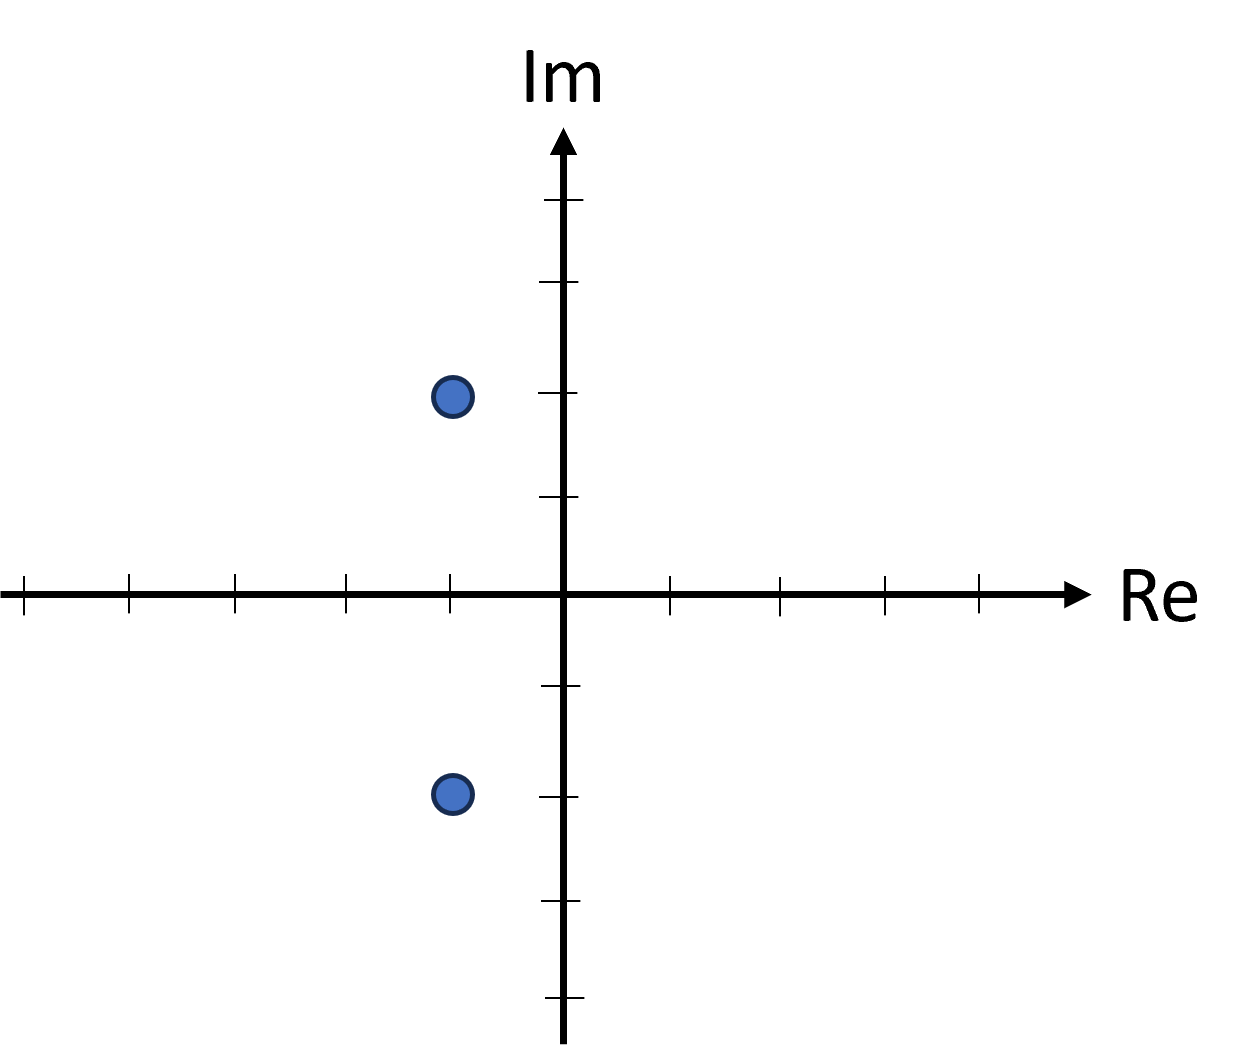
\includegraphics[width=5cm]{../Mathematik_2/Bilder/systemanalyse_konjugiert_komplexe_polstellen.png}
\end{center}

\item Was bedeutet das f�r das Zeitverhalten eines Systems? Das System ist asymptotisch stabil, weil die pyhsikalische L�sung f�r \(t\to \infty\) verschwindet.

\end{enumerate}

\end{exercisebox}

\begin{exercisebox}[Polstellen (�bertragungsfunktion Laplace)] % s = -1 pm 2i
Die folgende Skizze zeigt die Polstellen einer �bertragungsfunktion in der komplexen Ebene.

\begin{center}
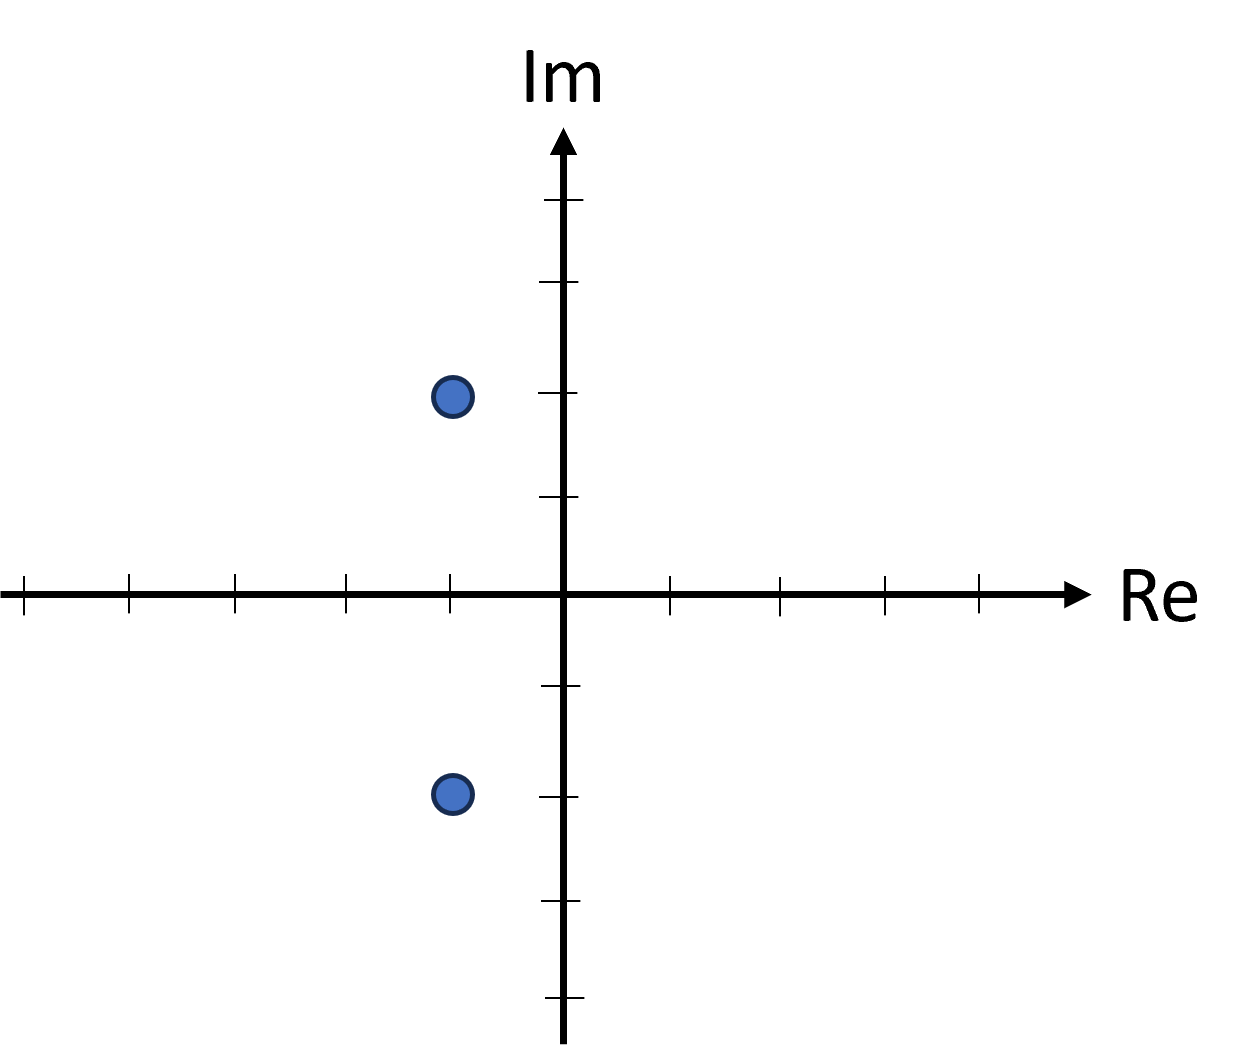
\includegraphics[width=5cm]{../Mathematik_2/Bilder/systemanalyse_konjugiert_komplexe_polstellen.png}
\end{center}

\begin{enumerate}
	\item Lesen Sie die Polstellen aus der Skizze ab. \(s_{1,2} = -1 \pm 2i\)
\item Geben Sie ein m�gliches Polynom an, das im Nenner der �bertragungsfunktion stehen k�nnte: \(p(s) = (s+1+ 2i)\cdot (s+1-2i)\).
\end{enumerate}

\end{exercisebox}



% Symboluebersicht: gemeinsame Quelle mit dem separaten Querformat-Handout.
\appendix
% Gemeinsame Quelle fuer Gesamtskript und eigenstaendige Symboluebersicht.
\begin{landscape}
\ifdefined\chapter
  \chapter{Symbol�bersicht Mathematik 2}
\else
  \section{Symbol�bersicht Mathematik 2}
\fi
\begingroup
\ifdefined\oldlongtable
  \let\longtable\oldlongtable
  \let\endlongtable\endoldlongtable
\fi
\setlength{\tabcolsep}{5pt}
\renewcommand{\arraystretch}{1.12}
\rowcolors{2}{white}{black!4}
\newcommand{\symbolgruppe}[1]{%
  \rowcolor{black!10}\multicolumn{3}{@{}l@{}}{\rule{0pt}{2.6ex}\textbf{#1}}\\*}
\begin{longtable}{@{}p{0.17\linewidth}p{0.35\linewidth}p{\dimexpr0.48\linewidth-4\tabcolsep\relax}@{}}
\caption{Zeichen und Notation in Mathematik 2}\label{MA2-Symbole}\\
\toprule
\textbf{Symbol} & \textbf{Bedeutung} & \textbf{Beispiel}\\
\midrule
\endfirsthead
\multicolumn{3}{@{}l@{}}{\textbf{Zeichen und Notation in Mathematik 2} -- Fortsetzung}\\
\toprule
\textbf{Symbol} & \textbf{Bedeutung} & \textbf{Beispiel}\\
\midrule
\endhead
\midrule
\multicolumn{3}{r@{}}{\footnotesize Fortsetzung auf der n�chsten Seite}\\
\endfoot
\bottomrule
\endlastfoot

\symbolgruppe{Grundnotation und Integration}
$a\stackrel{!}{=}b$ & Eine Gleichheit wird gefordert, etwa zur Bestimmung eines Parameters. & $2c\stackrel{!}{=}1\Rightarrow c=1/2$.\\
$\approx$ & N�herungsweise gleich; die Genauigkeit h�ngt vom Verfahren ab. & $\sqrt2\approx1{,}4142$.\\
$f'$, $f''$, $f^{(n)}$ & Erste, zweite bzw. $n$-te Ableitung; $f^{(n)}$ ist keine Potenz. & F�r $f(x)=x^3$ gilt $f''(x)=6x$ und $f^{(3)}(x)=6$.\\
$\dot y$, $\ddot y$ & Ableitungen nach der Zeit $t$. & $y(t)=\sin t\Rightarrow\dot y(t)=\cos t$, $\ddot y(t)=-\sin t$.\\
$\mathrm dx$ & Differential; kennzeichnet beim Integrieren die Integrationsvariable. & Bei $u=x^2$ ist $\mathrm du=2x\,\mathrm dx$.\\
$\int f(x)\,\mathrm dx$ & Unbestimmtes Integral: Familie der Stammfunktionen; die Integrationskonstante geh�rt dazu. & $\int x^2\,\mathrm dx=x^3/3+C$, $C\in\mathbb R$.\\
$F'=f$ & $F$ ist eine Stammfunktion von $f$. & $F(x)=x^3/3$ ist eine Stammfunktion von $f(x)=x^2$.\\
$\int_a^b f(x)\,\mathrm dx$ & Bestimmtes Integral; bei $a<b$ der vorzeichenbehaftete Fl�cheninhalt unter einem stetigen Graphen. & $\int_{-1}^{1}x\,\mathrm dx=0$.\\
$\int_a^b |f(x)|\,\mathrm dx$ & Geometrischer Fl�cheninhalt zwischen Graph und $x$-Achse, $a<b$. & $\int_{-1}^{1}|x|\,\mathrm dx=1$.\\
$[F(x)]_a^b$ & Kurzschreibweise f�r $F(b)-F(a)$. Bei stetigem $f=F'$ gilt der Hauptsatz. & $\int_0^1 x^2\,\mathrm dx=[x^3/3]_0^1=1/3$.\\
$\int_a^\infty f(x)\,\mathrm dx$ & Uneigentliches Integral: Grenzwert von $\int_a^b f(x)\,\mathrm dx$ f�r $b\to\infty$, sofern endlich. & $\int_0^\infty e^{-x}\,\mathrm dx=1$; $\int_0^b\cos x\,\mathrm dx=\sin b$ hat keinen Grenzwert.\\
$\int_{-\infty}^\infty f(x)\,\mathrm dx$ & Beide einseitigen uneigentlichen Integrale m�ssen einzeln konvergieren. & $\int_{-\infty}^{\infty}e^{-|x|}\,\mathrm dx=2$.\\
$L$ & L�nge eines differenzierbaren Funktionsgraphen auf $[a,b]$; hier $f\in C^1([a,b])$. & $L=\int_a^b\sqrt{1+(f'(x))^2}\,\mathrm dx$; f�r $f(x)=x$ auf $[0,1]$ ist $L=\sqrt2$.\\

\symbolgruppe{Reihen und Taylorapproximation}
$\sum_{k=0}^n a_k$ & Endliche Summe; $k$ ist der Summationsindex. & $\sum_{k=0}^3 2^k=1+2+4+8=15$.\\
$\sum_{k=0}^\infty a_k$ & Unendliche Reihe: Grenzwert der Partialsummen, falls dieser existiert. & $\sum_{k=0}^{\infty}(1/2)^k=2$.\\
$n!$ & Fakult�t: Produkt der Zahlen $1$ bis $n$; $0!:=1$. & $4!=24$, $\binom43=4!/(3!\,1!)=4$.\\
$\sum_{k=0}^\infty a_k(x-x_0)^k$ & Potenzreihe mit Entwicklungspunkt $x_0$. & $\sum_{k=0}^{\infty}x^k=1/(1-x)$ f�r $|x|<1$.\\
$R$ & Konvergenzradius: Konvergenz f�r $|x-x_0|<R$, Divergenz f�r $|x-x_0|>R$; Randpunkte separat pr�fen. & $\sum_{k=1}^{\infty}x^k/k$ hat $R=1$; bei $x=-1$ konvergent, bei $x=1$ divergent.\\
$p_n$, $T_n$ & Taylorpolynom vom Grad h�chstens $n$ am Entwicklungspunkt $x_0$. & $p_n(x)=\sum_{k=0}^n\frac{f^{(k)}(x_0)}{k!}(x-x_0)^k$; f�r $e^x$, $x_0=0$: $p_2(x)=1+x+x^2/2$.\\
$\sum_{k=0}^\infty\frac{f^{(k)}(x_0)}{k!}(x-x_0)^k$ & Taylorreihe von $f$. Sie stellt $f$ dort dar, wo $f$ mit dieser Reihe �bereinstimmt. & $e^x=\sum_{k=0}^{\infty}x^k/k!$ f�r alle $x\in\mathbb R$.\\
$R_n(x)$ & Restglied: Differenz zwischen Funktion und Taylorpolynom. & $R_n(x)=f(x)-p_n(x)$.\\
$\xi$, $M_{n+1}$ & Zwischenstelle zwischen $x_0$ und $x$ bzw. obere Schranke f�r $|f^{(n+1)}|$ auf dem verbindenden Intervall. & Bei hinreichender Glattheit: $R_n(x)=\frac{f^{(n+1)}(\xi)}{(n+1)!}(x-x_0)^{n+1}$ und $|R_n(x)|\leq\frac{M_{n+1}}{(n+1)!}|x-x_0|^{n+1}$.\\

\symbolgruppe{Funktionenr�ume und Orthogonalprojektion}
$\mathbb K$, $V$, $U\subseteq V$ & Skalark�rper, Vektorraum und Untervektorraum; im Skript auch $\mathbb V$, $\mathbb U$. & $\mathbb K=\mathbb R$ oder $\mathbb C$; $U=\operatorname{span}\{1,x\}\subset C([-1,1],\mathbb R)$.\\
$C([a,b],\mathbb R)$ & Raum der stetigen reellwertigen Funktionen auf $[a,b]$; auch $\mathcal C([a,b],\mathbb R)$. & $x\mapsto|x|$ liegt in $C([-1,1],\mathbb R)$.\\
$\mathcal R([a,b],\mathbb R)$ & Raum der Riemann-integrierbaren Funktionen auf $[a,b]$. & Eine st�ckweise stetige Funktion mit endlich vielen Spr�ngen ist Riemann-integrierbar.\\
$\mathcal P_n$ & Polynome vom Grad h�chstens $n$, einschlie�lich des Nullpolynoms. & $\mathcal P_2=\operatorname{span}\{1,x,x^2\}$.\\
$\langle f,g\rangle$ & Skalarprodukt auf einem geeigneten Funktionenraum; Intervall und Normierung sind zu beachten. & Auf $C([-1,1],\mathbb R)$: $\langle f,g\rangle=\int_{-1}^1 f(x)g(x)\,\mathrm dx$; $\langle1,x\rangle=0$.\\
$\|v\|$, $\|f\|$ & Vom Skalarprodukt erzeugte Norm: $\|v\|=\sqrt{\langle v,v\rangle}$. & F�r das obige Integral-Skalarprodukt: $\|x\|=\sqrt{2/3}$.\\
$\hat v$, $\hat f$ & Normierung eines von null verschiedenen Vektors bzw. einer Funktion. Ein Dach kann andernorts auch eine Fourier-Transformierte kennzeichnen. & $\hat v=v/\|v\|$; f�r $v=(i,0,1+i)^\top$ ist $\|v\|=\sqrt3$.\\
$\overline z$, $\overline{v}$ & Komplexe Konjugation; bei Vektoren komponentenweise. & $\overline{1+2i}=1-2i$; im komplexen Fourier-Skalarprodukt wird der zweite Faktor konjugiert.\\
$f\perp g$ & Orthogonalit�t: Das Skalarprodukt ist null. & Auf $[-1,1]$: $\int_{-1}^1 1\cdot x\,\mathrm dx=0$.\\
$\operatorname{proj}_U v$ & Orthogonalprojektion auf einen endlichdimensionalen Unterraum $U$ mit Orthonormalbasis $(e_j)$. & $\operatorname{proj}_U v=\sum_j\langle v,e_j\rangle e_j$; das Residuum $v-\operatorname{proj}_U v$ ist orthogonal zu $U$.\\
$A^\top A x_*=A^\top b$ & Normalengleichung zur reellen Ausgleichsrechnung; bei vollem Spaltenrang ist $x_*$ eindeutig. & $x_*$ minimiert $\|Ax-b\|^2$; $A^\top(b-Ax_*)=0$.\\

\symbolgruppe{Fourierreihen und diskrete Fouriertransformation}
$T$, $\omega_0$ & Periode und zugeh�rige Grundkreisfrequenz $\omega_0=2\pi/T$. Die kleinste positive Periode hei�t Grundperiode. & $\sin(3t)$ hat Grundperiode $T=2\pi/3$ und $\omega_0=3$.\\
$\mathcal P_T$ & Raum der $T$-periodischen Funktionen: $f(t+T)=f(t)$; $T$ muss nicht die kleinste Periode sein. & $t\mapsto\sin(2\pi nt/T)\in\mathcal P_T$ f�r $n\in\mathbb N^+$.\\
$\omega_k=k\omega_0$ & Diskrete Kreisfrequenzen; $k$ bezeichnet die Harmonische. & $T=2\pi\Rightarrow\omega_k=k$.\\
$a_0,a_k,b_k$ & Reelle Fourierkoeffizienten in $a_0/2+\sum_{k\geq1}(a_k\cos(k\omega_0t)+b_k\sin(k\omega_0t))$. & $a_k=\frac2T\int_0^T f(t)\cos(k\omega_0t)\,\mathrm dt$, $k\geq0$; f�r $b_k$ Sinus statt Kosinus, $k\geq1$.\\
$c_k$, $k\in\mathbb Z$ & Komplexe Fourierkoeffizienten; die Reihe lautet $\sum_{k\in\mathbb Z}c_ke^{ik\omega_0t}$. & $c_k=\frac1T\int_0^T f(t)e^{-ik\omega_0t}\,\mathrm dt$; f�r $k\geq1$: $c_k=(a_k-i b_k)/2$, $c_0=a_0/2$.\\
$N$, $t_n$, $u_n$ & Anzahl der Samples, Abtastzeitpunkte und Signalwerte im Beobachtungsfenster der L�nge $T$, beginnend bei $0$. & $t_n=nT/N$, $u_n=u(t_n)$, $n=0,\ldots,N-1$.\\
$W_N=e^{-2\pi i/N}$ & F�r die DFT verwendete $N$-te Einheitswurzel; $W_N^N=1$. & $W_4=-i$; seine Potenzen sind $1,-i,-1,i$.\\
$\tilde c_k$ & Diskrete Fourierkoeffizienten in der Normierung des Skripts. & $\tilde c_k=\sum_{n=0}^{N-1}u_nW_N^{kn}$; f�r $(u_0,u_1)=(1,3)$ ist $(\tilde c_0,\tilde c_1)=(4,-2)$.\\
$\operatorname{iDFT}$ & Inverse diskrete Fouriertransformation; der Faktor $1/N$ steht hier bei der R�cktransformation. & $u_n=\frac1N\sum_{k=0}^{N-1}\tilde c_kW_N^{-kn}$; aus $(4,-2)$ wird wieder $(1,3)$.\\
$T_N$ & DFT-Matrix mit Eintr�gen $(T_N)_{kn}=W_N^{kn}$, $k,n=0,\ldots,N-1$. & $T_2=\begin{pmatrix}1&1\\1&-1\end{pmatrix}$; $T_2^{-1}=\tfrac12T_2$.\\

\symbolgruppe{Fouriertransformation und Laplacetransformation}
$\hat f$, $\mathcal F(f)$ & Fourier-Transformierte; hier symmetrische Normierung. Das Integrationssymbol verwendet dieselbe Variable wie $f$. & $\hat f(\omega)=\frac1{\sqrt{2\pi}}\int_{-\infty}^{\infty}f(t)e^{-i\omega t}\,\mathrm dt$.\\
$\omega$ & Kontinuierliche Kreisfrequenz, im Unterschied zu den diskreten $\omega_k$. & F�r $f(t)=e^{-|t|}$ ist $\hat f(\omega)=\sqrt{2/\pi}/(1+\omega^2)$.\\
$\mathcal F^{-1}$ & Inverse Fouriertransformation; die Formel gilt unter geeigneten Integrabilit�ts- und Regularit�tsbedingungen. & $f(t)=\frac1{\sqrt{2\pi}}\int_{-\infty}^{\infty}\hat f(\omega)e^{i\omega t}\,\mathrm d\omega$.\\
$Y(s)$, $\mathcal L(y)(s)$ & Einseitige Laplace-Transformierte; $s$ ist im Allgemeinen komplex, der Konvergenzbereich ist anzugeben. & $Y(s)=\int_0^\infty y(t)e^{-st}\,\mathrm dt$; f�r $y(t)=1$ gilt $Y(s)=1/s$, $\operatorname{Re}s>0$.\\
$H(t)$ & Heaviside-Funktion: hier $0$ f�r $t<0$ und $1$ f�r $t\geq0$. & $\mathcal L(H(t-a)\cos(t-a))(s)=e^{-as}s/(s^2+1)$ f�r $a>0$, $\operatorname{Re}s>0$.\\
$f\star g$ & Faltung; bei kausalen Funktionen gen�gt ein Integral von $0$ bis $t$, $t\geq0$. & $(f\star g)(t)=\int_0^t f(t-\tau)g(\tau)\,\mathrm d\tau$; $f(t)=g(t)=1$ f�r $t\geq0$ liefert $(f\star g)(t)=t$.\\

\symbolgruppe{Differentialgleichungen, Numerik und Systemanalyse}
$y'=f(y,x)$ & Explizite Differentialgleichung erster Ordnung; die Reihenfolge der Argumente von $f$ ist hier festgelegt. & $f(y,x)=y+x^2$ bedeutet $y'=y+x^2$.\\
$y(x_0)=y_0$ & Anfangsbedingung; zusammen mit der Differentialgleichung ein Anfangswertproblem. & $y'=y$, $y(0)=1$ hat die L�sung $y(x)=e^x$.\\
$h$, $x_k$, $y_k$ & Schrittweite, Gitterpunkt $x_k=x_0+kh$ und N�herung $y_k\approx y(x_k)$. & Explizites Euler-Verfahren: $y_{k+1}=y_k+h f(y_k,x_k)$.\\
$\dot{\boldsymbol x}=A\boldsymbol x$ & Lineares homogenes System mit konstanter Matrix $A$. & F�r $A=\operatorname{diag}(-1,-2)$ gilt $\boldsymbol x(t)=(c_1e^{-t},c_2e^{-2t})^\top$.\\
$\lambda$, $v$ & Eigenwert und zugeh�riger Eigenvektor $v\neq0$: $Av=\lambda v$. & Dann ist $\boldsymbol x(t)=e^{\lambda t}v$ eine L�sung von $\dot{\boldsymbol x}=A\boldsymbol x$.\\
$\det(A-\lambda I)$ & Charakteristisches Polynom; seine Nullstellen sind die Eigenwerte von $A$. & $A=\operatorname{diag}(-1,-2)$ liefert $(\lambda+1)(\lambda+2)$ mit Nullstellen $-1,-2$.\\
$\operatorname{Re}\lambda$ & Realteil eines Eigenwerts. Sind alle Realteile negativ, ist das konstante lineare System asymptotisch stabil. & $\lambda_{1,2}=-1\pm2i$ beschreiben ged�mpfte Schwingungen.\\
$H(s)$ & �bertragungsfunktion eines linearen zeitinvarianten Systems bei verschwindenden Anfangsbedingungen; von $H(t)$ oben zu unterscheiden. & Aus $\dot y+2y=u$ folgt $H(s)=Y(s)/U(s)=1/(s+2)$.\\
$H(i\omega)$ & Frequenzgang: �bertragungsfunktion auf der imagin�ren Achse, sofern dort definiert. & F�r $H(s)=1/(s+2)$ gilt $|H(i\omega)|=1/\sqrt{4+\omega^2}$.\\

\end{longtable}
\endgroup
\end{landscape}


\end{document}
